\documentclass[a4j,10pt]{jsarticle}
\usepackage[dvipdfmx,hiresbb]{graphicx}
% 画像は img/ 配下へ集約した（2026-09-05）。\includegraphics はファイル名だけで書いてよい。
%   img/scan/ … 問題編のページスキャン（prob_p*, prob2_p*）
%   img/text/ … 講義編から切った図（text_p*, text2_p*）
%   fig/      … TeX化のときに切り出した図（こちらは fig/ 付きで参照している）
\graphicspath{{./}{img/text/}{img/scan/}{fig/}}
\usepackage{amsmath,amssymb}
%\usepackage{fancybox}
 \usepackage{ascmac}
 \usepackage{multicol}
 \usepackage{multicol,multienum}
 \usepackage{latexsym}
 \usepackage{wrapfig}
% \usepackage{tcolorbox}
\usepackage{eclbkbox}
\usepackage[dvipdfmx]{color}
\usepackage{butsuri_style}   % 紙面デザイン（2026-08-31 全章に適用）
%
% ######## measure #########
% # mm = 1mm = 2.85pt      #
% # cm = 10mm = 28.5pt     #
% # in = 25.4mm = 72.27pt  #
% # pt = 0.35mm = 1pt      #
% # em = width of [M]      #
% # ex = height of [x]     #
% # zw = width of [Kanji]  #
% # zh = height of [Kanji] #
% ##########################
% ##################### Portrait Setting #########################
% # TOP = 1inch + \voffset + \topmargin + \headheight + \headsep #
% #     = 1inch + 0pt + 4pt + 20pt + 18pt (default)              #
% # BOTTOM = \paperheight - TOP -\textheight                     #
% ################################################################
\setlength{\textheight}{\paperheight}   % 紙面縦幅を本文領域にする（BOTTOM=-TOP）
\setlength{\topmargin}{-5truemm}       % 上の余白を30mm（=1inch+4.6mm）に
\addtolength{\topmargin}{-\headheight}  % 
\addtolength{\topmargin}{-\headsep}     % ヘッダの分だけ本文領域を移動させる
\addtolength{\textheight}{-50truemm}    % 下の余白も30mm（BOTTOM=-TOPだから+TOP+30mm）
% #################### Landscape Setting #######################
% # LEFT = 1inch + \hoffset + \oddsidemargin (\evensidemargin) #
% #      = 1inch + 0pt + 0pt                                   #
% # RIGHT = \paperwidth - LEFT - \textwidth                    #
% ##############################################################
\setlength{\textwidth}{\paperwidth}     % 紙面横幅を本文領域にする（RIGHT=-LEFT）
\setlength{\oddsidemargin}{-0.4truemm}  % 左の余白を25mm(=1inch-0.4mm)に
\setlength{\evensidemargin}{-0.4truemm} % 
\addtolength{\textwidth}{-50truemm}     % 右の余白も25mm（RIGHT=-LEFT）
\setlength{\footskip}{20truemm}        %ページ番号の位置を指定
%
%
%%%%%%    TEXT START    %%%%%%
\begin{document}
\newcounter{nombre} %必須
\renewcommand{\thenombre}{\arabic{nombre}} %任意
\setcounter{nombre}{0} %任意

\newcommand{\ex}[1][]{\refstepcounter{nombre}#1【例題 \thenombre】}

\newcounter{nomber} %必須
\renewcommand{\thenomber}{\arabic{nomber}} %任意
\setcounter{nomber}{0} %任意

\newcommand{\prob}[1][]{\refstepcounter{nomber}#1【問題 \thenomber】}

\newcommand{\MARU}[1]{{\ooalign{\hfil#1\/\hfil\crcr\raise.167ex\hbox{\mathhexbox20D}}}}

%%%%%%%%%% 練習問題・解答を TeX 化するためのマクロ（2026-08-29 追加）%%%%%%%%%%
\newcounter{qno}                        % ［１］［２］… 問題の通し番号（章をまたいで連番）
% A問題／B問題／C問題 の見出し
\newcommand{\Rank}[1]{\par\medskip\noindent{\gtfamily #1}\par\nobreak\vspace{1mm}}
% ［N】【タイトル】  第2引数を付けると「指定問題」バッジが出る
\newcommand{\Mon}[1]{\filbreak\refstepcounter{qno}\MonN{\theqno}{#1}}
% 解答側など，番号を明示して見出しを出す場合
\newcommand{\MonN}[2]{\par\vspace{2mm}\noindent{\gtfamily ［#1］【#2】}}
\newcommand{\Sitei}{\hspace{0.5zw}\colorbox[gray]{0.85}{\footnotesize 指定問題}}
% 単位（数式モードで使う）  例: $200\U{m}$
\newcommand{\U}[1]{\,[\mathrm{#1}]}
% 摂氏温度（\U と同じ体裁。数式モードで使う）  例: $20\Cel$
\newcommand{\Cel}{\,[{}^\circ\mathrm{C}]}
% 「……答」マーク
% 「……（答）」は途中で改行させない（\mbox で一塊にする）
\newcommand{\Ans}{\ifmmode\ \cdots\text{(答)}\else\nobreak\hspace{0.25zw}\mbox{$\cdots$(答)}\fi}
% 式番号（……①）も同様に一塊
\newcommand{\Eq}[1]{\ifmmode\ \cdots\MARU{#1}\else\nobreak\hspace{0.25zw}\mbox{$\cdots$\MARU{#1}}\fi}
% 小問 (1)(2)… のぶら下げリスト
\newenvironment{komon}{%
  \begin{list}{}{%
    \setlength{\leftmargin}{2.2zw}\setlength{\labelwidth}{1.9zw}%
    \setlength{\labelsep}{0.5zw}\setlength{\itemsep}{0pt}%
    \setlength{\parsep}{0pt}\setlength{\topsep}{2pt}\setlength{\partopsep}{0pt}}%
}{\end{list}}
\newcommand{\ko}[1]{\item[{\makebox[1.9zw][r]{(#1)}}]}
% 図を本文の右に置く（wrapfigure は連続使用で衝突するため minipage を使う）
% 使い方: \begin{zuright}{図の幅} 本文 \zusep 図 \end{zuright}
\newenvironment{zuright}[1]{%
  \par\medskip\setlength{\zuw}{#1}%
  \noindent\begin{minipage}[t]{\dimexpr\linewidth-\zuw-4mm\relax}%
}{\end{minipage}\par\medskip}
\newlength{\zuw}
\newcommand{\zusep}{\end{minipage}\hfill\begin{minipage}[t]{\zuw}\vspace{0pt}\centering}

% 【指針】は太枠，【別解】【注】は細枠
\newenvironment{sisin}{\setlength{\fboxrule}{1.2pt}\begin{itembox}[l]{【指針】}}{\end{itembox}}
\newenvironment{bekkai}{\begin{itembox}[l]{【別解】}}{\end{itembox}}
\newenvironment{chuu}{\begin{itembox}[l]{【注】}}{\end{itembox}}

%%%%%%%%%% 例題まわりの体裁（2026-08-29 追加）%%%%%%%%%%
% 地の文＝枠なし／例題＝太枠／KEY・解答＝細枠、で役割が一目で分かるようにする
% 例題の問題文（原本と同じ太枠＋左上に【例題 N】〈タイトル〉）
\newenvironment{reidai}[1]{\par\medskip\setlength{\fboxrule}{1.2pt}%
  \begin{itembox}[l]{\ex〈#1〉}}{\end{itembox}}
% 例題の【指針】は枠なし（地の文と解答の中間の位置づけ）
\newenvironment{sisinE}{\par\medskip\noindent{\gtfamily 【指針】}\par\nobreak
  \begingroup\leftskip=1zw\noindent\ignorespaces}{\par\endgroup\medskip}
% 【KEY】は原本どおり細枠
\newenvironment{key}{\setlength{\fboxrule}{0.4pt}\begin{itembox}[l]{【KEY】}}{\end{itembox}}
% 【解答】は長くなるので改ページできる breakbox を使う
\newenvironment{kaitou}{\par\medskip\begin{breakbox}\noindent{\gtfamily 【解答】}\par\nobreak}{\end{breakbox}\par\medskip}
%%%%%%%%%%%%%%%%%%%%%%%%%%%%%%%%%%%%%%%%%%%%%%%%%%%%%%%%%%%%
%%%%%%%%%%%%%%%%%%%%%%%%%%%%%%%%%%%%%%%%%%%%%%%%%%%%%%%%%%%%%%%%%%%%%%%%%%%%


\def\heiko{\mathrel{\raise.3ex\hbox{\scalebox{.7}{%
    \rotatebox[origin=c]{-7}{/}%
    \kern-.35em\rotatebox[origin=c]{-7}{/}}}}}%

%%%%% 紙面デザインを有効にする（2026-08-31）
%%%%% \Rank \Mon reidai sisin kaitou … は上で \begin{document} の“後”に定義しているため，
%%%%% butsuri_style の読み込み時には再定義できない．ここで \ButsuriApply を呼んで差し替える．
\ButsuriApply

\newpage

{\huge 入試物理基礎演習}
\vspace{5mm}

{\bf【学習目標】}

このプリントは，物理の全範囲を基礎から解説し，東大をはじめとする難関大学に現役合格するための基盤作りを目標としています．

各単元ごとに重要事項や解き方のポイントをまとめ，その単元の練習問題と解答を載せてあります．一読してもよく分からない部分も出てくると思いますが，問題の解説を熟読し，場合によっては教科書などを参考にしてください．

各単元の練習問題は繰り返し解き，必ず解けるようにしてください．
A問題，B問題，C問題とレベル分けしてあります．

A問題は，法則や基本事項を単純に用いるだけの問題です．この問題で躓くときは，講義部分の解説や参考書などを確認し，覚えるべき法則の再確認をしてください，

B問題は，重要な典型問題です．答え合わせをする際は，答えのみがあっているかどうかを見るのではなく，途中の考え方まで含めてあっていたかどうか，掲載されている【指針】【解答】を熟読しましょう．

C問題は，入試レベルの問題で現時点では独力で解答するのは難しいかもしれません．
そうした際，すぐに諦めるのではなく，なんとか基本問題を応用して解けないか試行錯誤してみてください．
こちらも詳しい【指針】【解答】がついているので，できる限り理解するよう努力することが重要です．

なお，問題の中で，最も優先すべき問題を2題を選んで指定問題の印がついてあります．
どうしても学習時間が確保できない場合は，この指定問題2問にしぼって取り組むと良いでしょう．

問題に取り組む際は，以下の点に注意してください．
\begin{description}
\item[(1)] $物理法則・原理を正しく覚えること．$
\item[(2)] $なぜその法則が成り立つのかを考えて問題を解くこと．$
\end{description}

物理という科目は，覚えることはほとんどありません．
最低限の原理を覚えてしまえば，あとは数学的に導いていくことができます．
そのため，問題の解き方を覚えるのではなく，なぜそのような現象が起こるのか，なぜそのように解けるのかを理解するように意識していきましょう．




\vspace{5mm}
%{\bf【宿題】}

%（1）例題解き直し
%
%授業で解説した例題は，家に帰ってから必ずその日のうちに解き直しを行ってください．
%解き直しは，解説を読まずに，問題を見て解答を作れるか自分でテストします．
%もし解けなければ，解説を読んで，再度解いてみてください．
%自力で解答が再現できるようになるまで繰り返すことが解き直しです．
%
%\vspace{1mm}
%
%（2）練習問題
%
%授業で解説した例題の練習問題を載せてあります．
%授業では解説しませんが，習ったことが定着したか確認してください．
%次回の授業までに行いましょう．

{\bf【やり方】}

%以下の点に注意して進めてください．

・図や途中経過もできるだけノートに書く

・丸付けも行う

・間違えた問題は赤字で解き直す（間違えた答案は消さずに取っておく）

・わからなかった問題は解答をよく読んで理解し，その上で赤で解答を写しておく
\newpage
\tableofcontents
\newpage

  \ 
  
\newpage
\include{physics_ch1}
\include{physics_ch2}
 \ 
 
\newpage
\section{物体に作用する力とつり合い}

\subsection{力のつり合いと運動の法則}

物体に力が働く（=作用する）と，物体は変形したり，その運動状態が変化したりする．
すなわち，{\bf 物体の状態はその物体に作用している力によって定まる．}
よって，物体に作用する力を把握することが重要である．

力は加える向きと，加える大きさの2つを持つので，$\overrightarrow{f}や\overrightarrow{F}$などとベクトルを用いて表す．
この表し方を用いて，ある物体に作用する2つの力をベクトル合成により1つにまとめたり（合力），もしくは1つの力を成分分解により2つの力に分解したりすることができる．


\begin{figure}[h]
\begin{center}
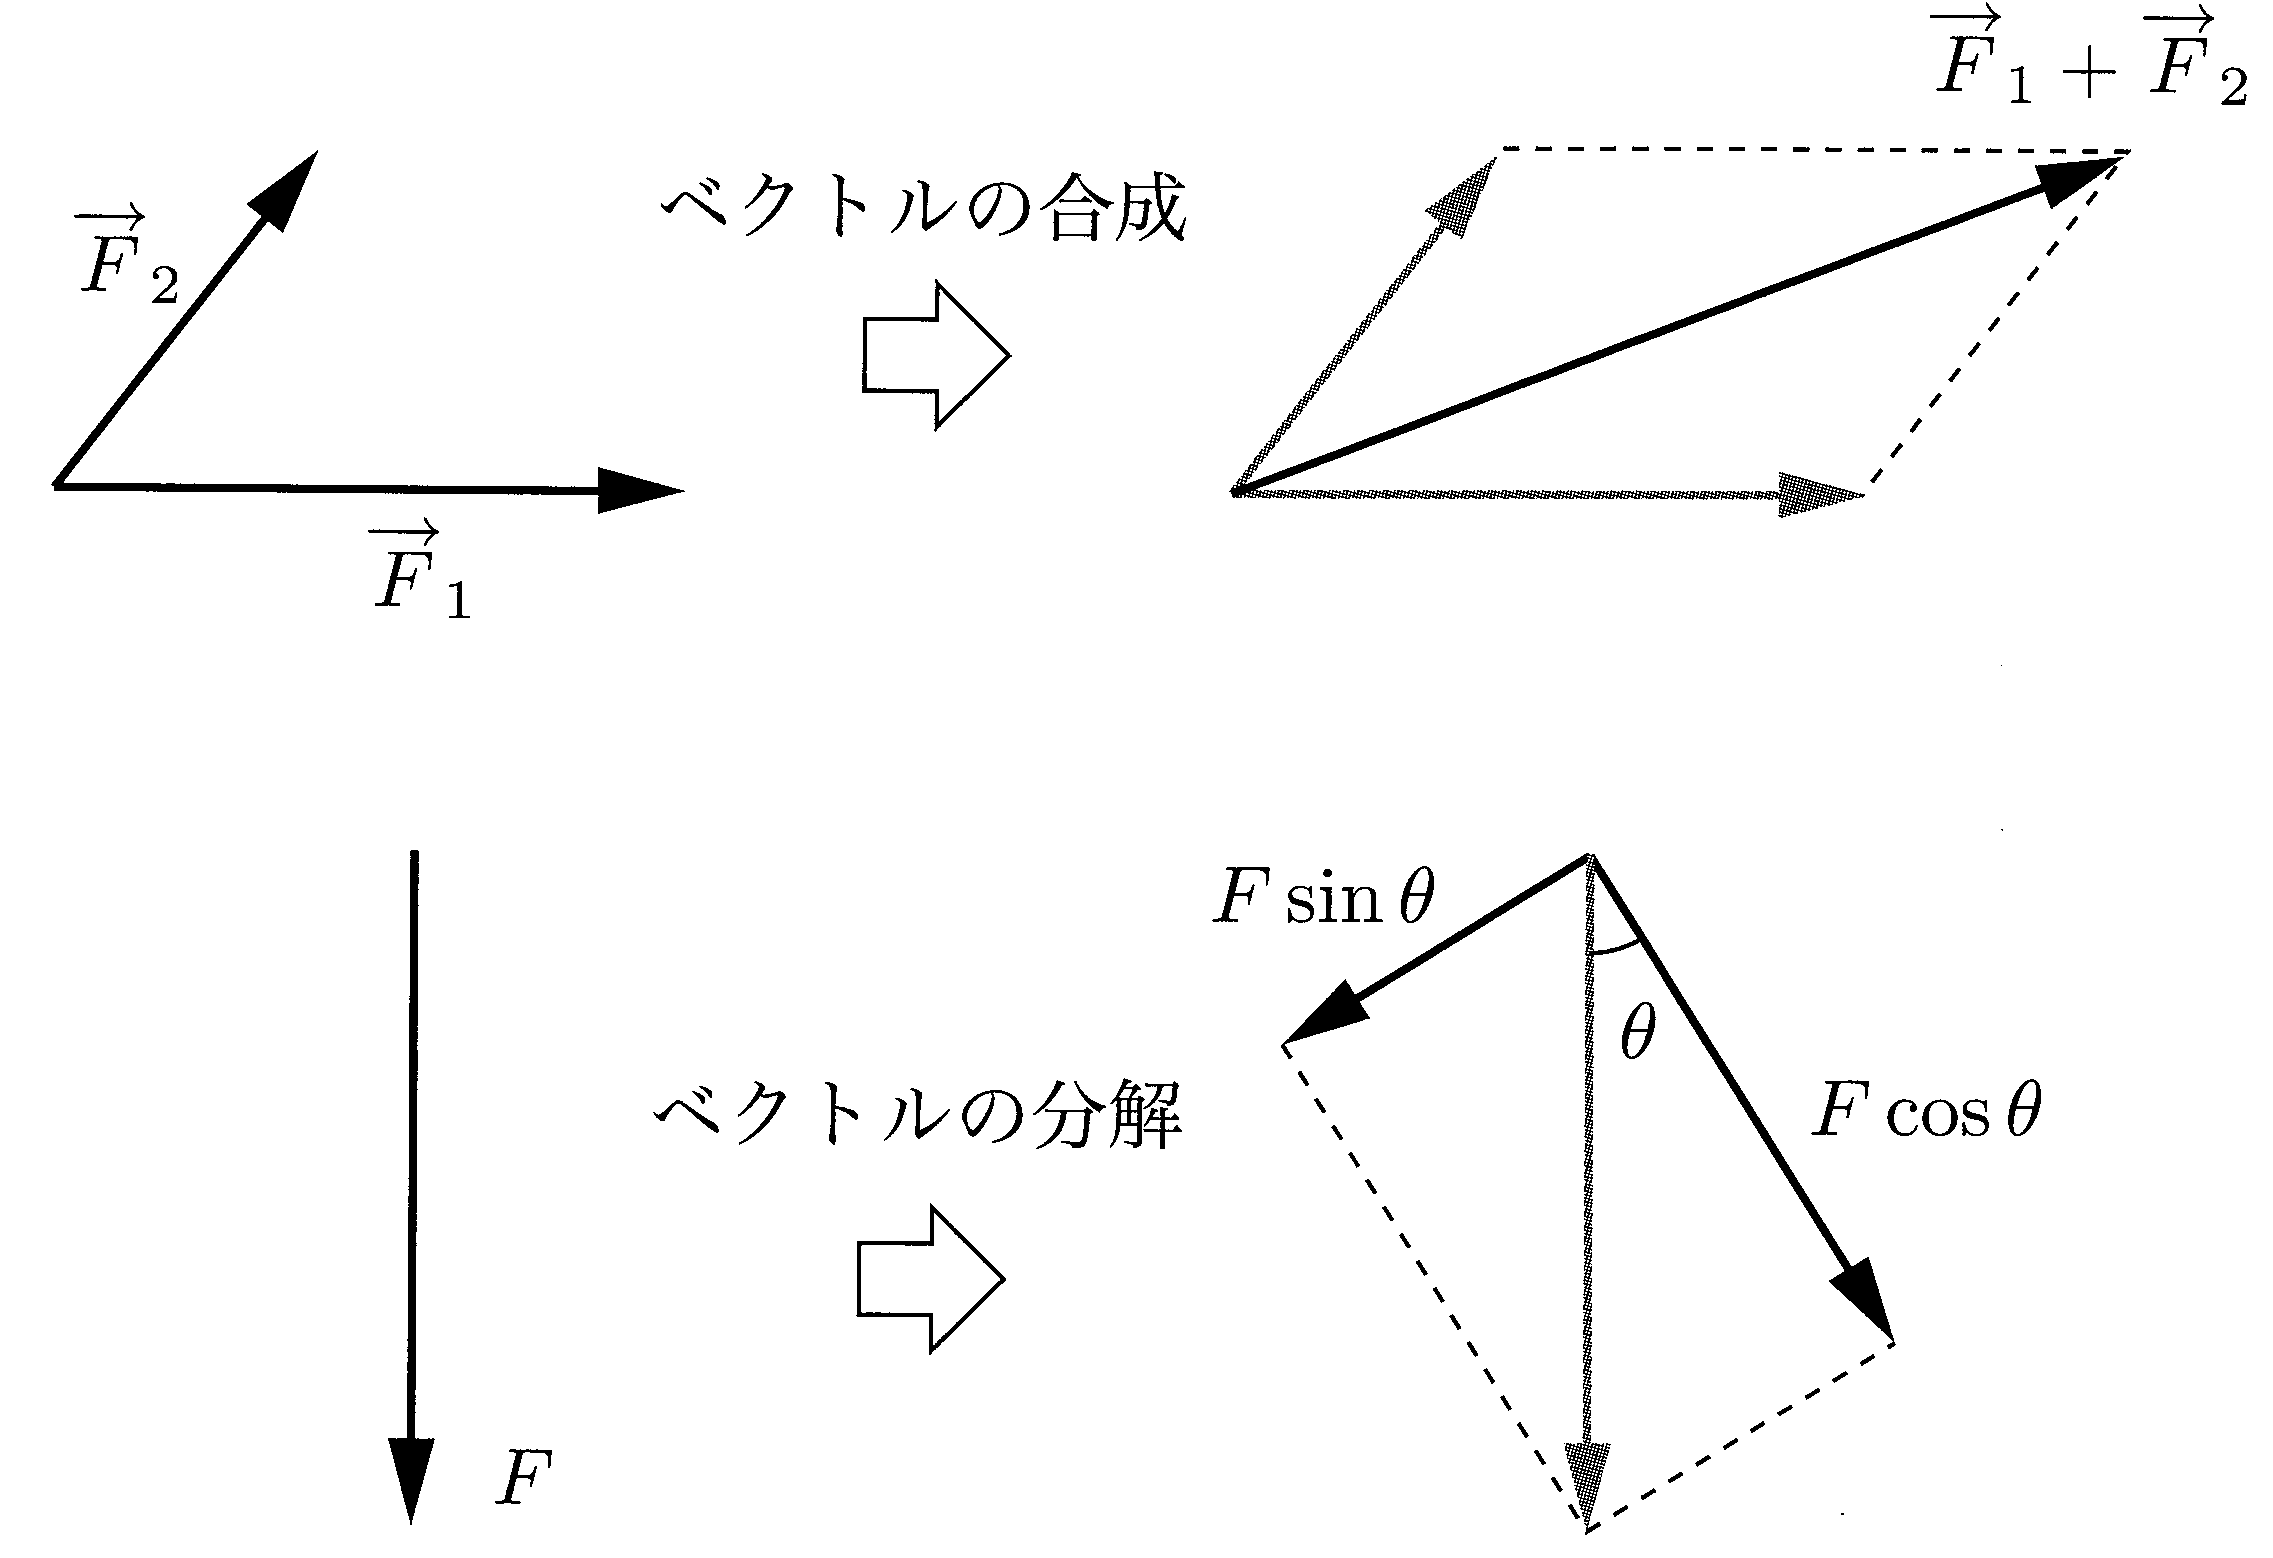
\includegraphics[width=100mm]{text_p14_fig1.png}
\end{center}
\end{figure}

物体に作用するすべての力の合力が$\overrightarrow{0}$であるとき，{\bf 力がつり合っている}という．
このとき，静止している物体は静止し続け，動いている物体はその速度を維持し続けて等速度直線運動を行う．
これを{\bf 慣性の法則（運動の第一法則）}という．
この慣性の法則をはじめ，運動に関する性質をまとめたものを{\bf ニュートンの運動の法則}という．

\begin{matome}{運動の法則}
 $\hspace{10mm}{\bf 第一法則　慣性の法則}\\
 \hspace{15mm} 物体に作用する力の合力が\overrightarrow{0}{\rm [N]}となる場合，物体は静止または等速度運動を行う．\\
 \hspace{10mm}{\bf 第二法則　運動方程式}\\
 \hspace{15mm} 物体に作用する力の合力を\overrightarrow{F}{\rm [N]}とすれば，物体は加速度運動を行い，質量をm{\rm [kg]}，\\ \hspace{15mm}加速度を\overrightarrow{a} {\rm [m/s^2]}とすると，m\overrightarrow{a}=\overrightarrow{F}が成立する．\\
  \hspace{10mm}{\bf 第三法則　作用反作用の法則}\\
 \hspace{15mm} 物体Aが物体Bに力を及ぼすとき，物体Aは物体Bから等大逆向きの力を受ける．$
\end{matome}

\newpage
\subsection{力学問題の基本的な解法}

以上の運動の法則に基づいて，力学の問題は以下の手順に従って解くことが基本となる．
\begin{matome}{力学問題の基本的な解法}
 $\hspace{10mm}{\bf \MARU{1}　各物体に作用している力を描き出す}\\
 \hspace{15mm} \underline{ポイント}　・場の力以外は接触しているものからしか力を受けない．\\
 \hspace{32mm} ・複数物体がある場合は各物体ごとに別々に描くと良い．\\
 \hspace{10mm}{\bf \MARU{2}　各方向ごとに運動方程式または力のつり合いを立てる}\\
 \hspace{15mm} \underline{ポイント}　・必要に応じてx軸，y軸を設定し，力をそれぞれの成分に分解する．\\
 \hspace{32mm} ・極力分解する力，または加速度が少なくなる方向を選ぶ．\\ 
 \hspace{10mm}{\bf \MARU{3}　式を連立して未知数について解く}\\
 \hspace{15mm} \underline{ポイント}　・どれが未知数なのかを意識して式変形していく．\\
 \hspace{32mm} ・未知数の数に対して式の数が足りない場合は，束縛条件やまだ使っていない\\\hspace{33mm}問題文中に与えられている条件がないかを探してみる．\\
  \hspace{10mm}{\bf \MARU{4}　設問に応じて運動を解析する}\\
 \hspace{15mm} \underline{ポイント}　・等加速度運動となる場合，v=v_0+at,\hspace{1mm}x=x_0+v_0t+\dfrac{1}{2}at^2,\hspace{1mm}v^2-v_0^2=2a(x-x_0)\\ \hspace{33mm}といった公式を利用して時間や位置を求める．$
\end{matome}

%\newpage
\subsection{力の種類}

物体に作用する力にはさまざまなものがあるが，次の2種類に分けて考えていくと良い．

% 誤植訂正（2026-08-29）：節「力の種類」の箱に前節の見出しが残っていたため修正．
\begin{matome}{力の種類}
$ \hspace{10mm}{\bf \MARU{1}　場の力：物体が場から受ける力，および見かけの力}\\
 \hspace{20mm} 重力，万有引力，クーロン力，電場による力，慣性力\\
 \hspace{10mm}{\bf \MARU{2}　接触力：接触している物体からは必ず力を受ける}\\
 \hspace{20mm} 弾性力，張力，垂直抗力，静止摩擦力，動摩擦力，浮力など\\
 \hspace{15mm} 作用反作用に注意して物体ごとに力の作用図を描くようにすること．$
\end{matome}

これらの力について順番に見ていくことにする．
なお，力の単位は[kg],[m],[s]を用いると${\rm [kg・m/s^2]}$と表されるが，通常はこれを[N]（ニュートン）と書く．

\newpage
\fbox{1} 重力

\begin{wrapfigure}[5]{r}[5mm]{30mm}
  \centering
  \vspace{-5mm}
  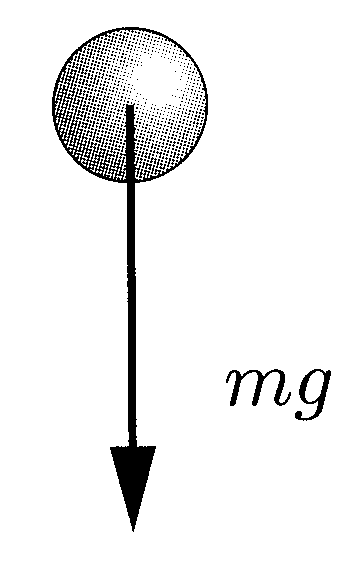
\includegraphics[keepaspectratio,width=20mm]
  {text_p16_fig1.png}
\end{wrapfigure}

あらゆるものは万有引力を受けるが，地表付近の物体に関しては地球から受ける万有引力のみを考えればよく，その力は場所によらず一定であるとして良い．
重力加速度の大きさを$g [{\rm m/s^2}]$とすれば，質量$m$[kg]の物質に作用する重力の大きさは$mg$[N]となり，向きは鉛直下向きとなる．\vspace{10mm}

\fbox{2} 垂直抗力

\begin{wrapfigure}[10]{r}[5mm]{60mm}
  \centering
  \vspace{-5mm}
  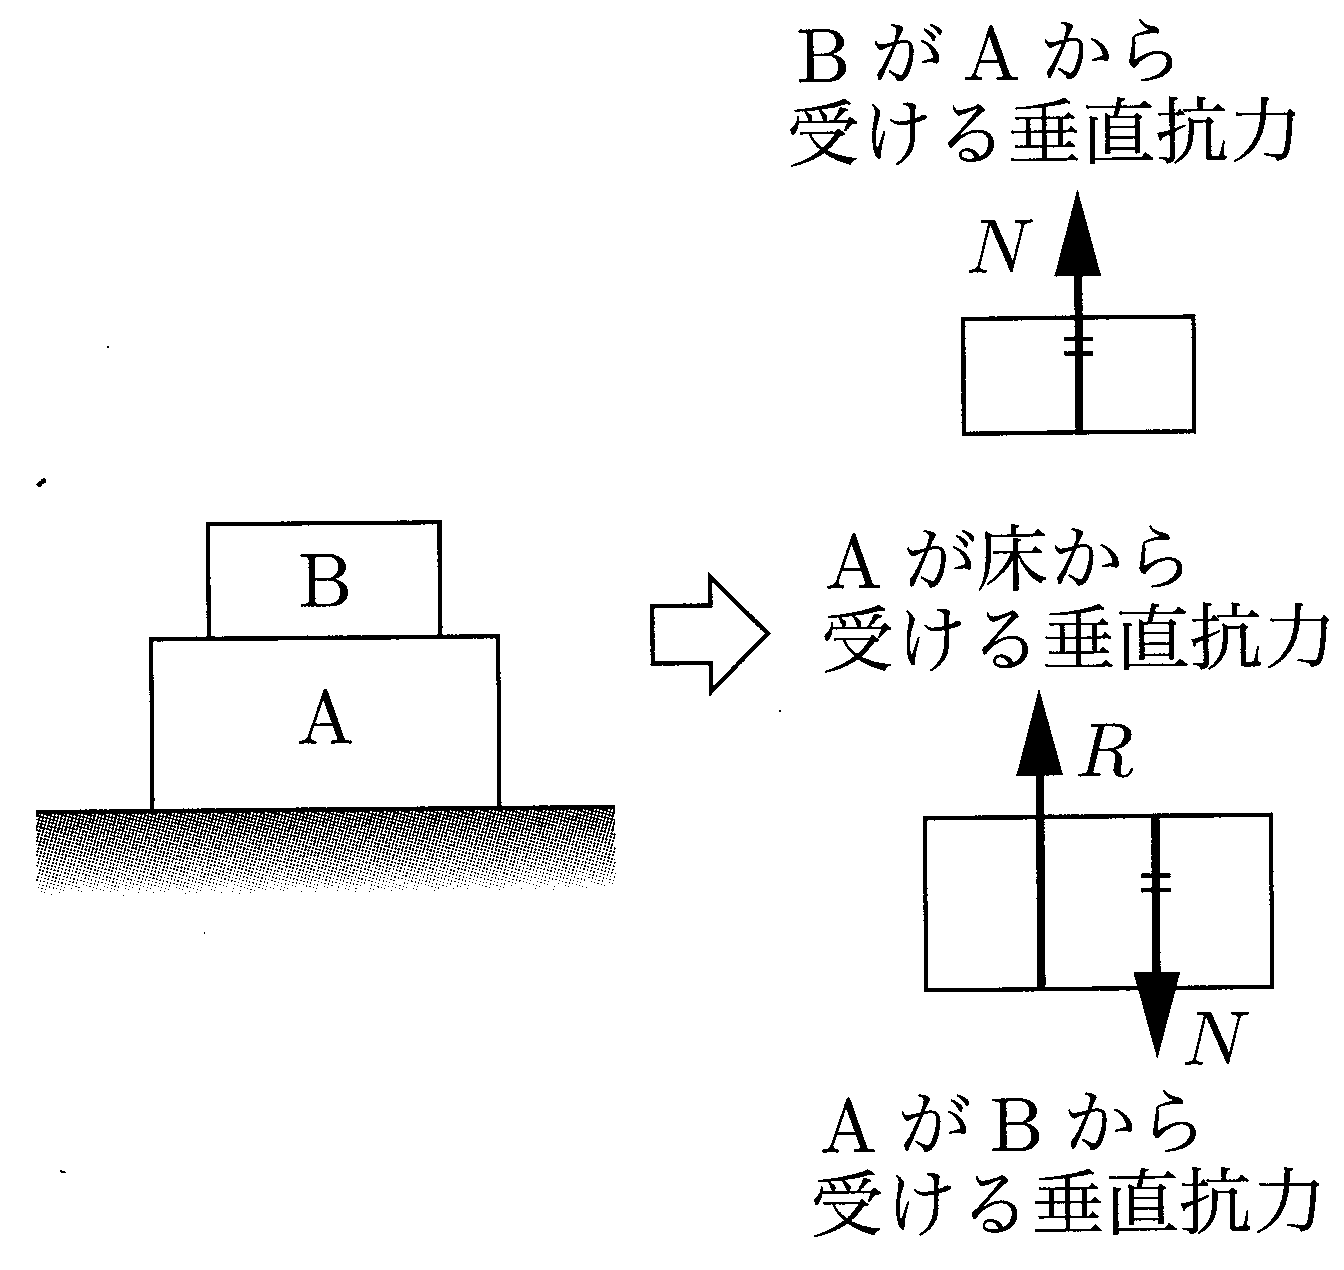
\includegraphics[keepaspectratio,width=50mm]
  {text_p16_fig2.png}
\end{wrapfigure}

接触している物体同士には垂直抗力が作用する．
向きは接触面に対して垂直な方向で，{\bf 大きさは未知量として扱い，力のつり合いや運動方程式をもとに計算する．}
$物体Aと物体Bが接触している場合，作用・反作用の法則よりAがBから受ける垂直抗力と，BがAから受ける垂直抗力は等大逆向きとなる．$
$AとB$が接触しているための条件は，力のつり合いの式や運動方程式によって計算して求められた垂直抗力の大きさ$N$[N]が実際に存在する，つまり{\bf 2物体が離れない条件は，2物体間に作用する垂直抗力の大きさ}\mbox{\boldmath $N$}{\bf が負でないこと}である．\vspace{10mm}


\fbox{3} 張力

\begin{wrapfigure}[5]{r}[5mm]{60mm}
  \centering
  \vspace{-5mm}
  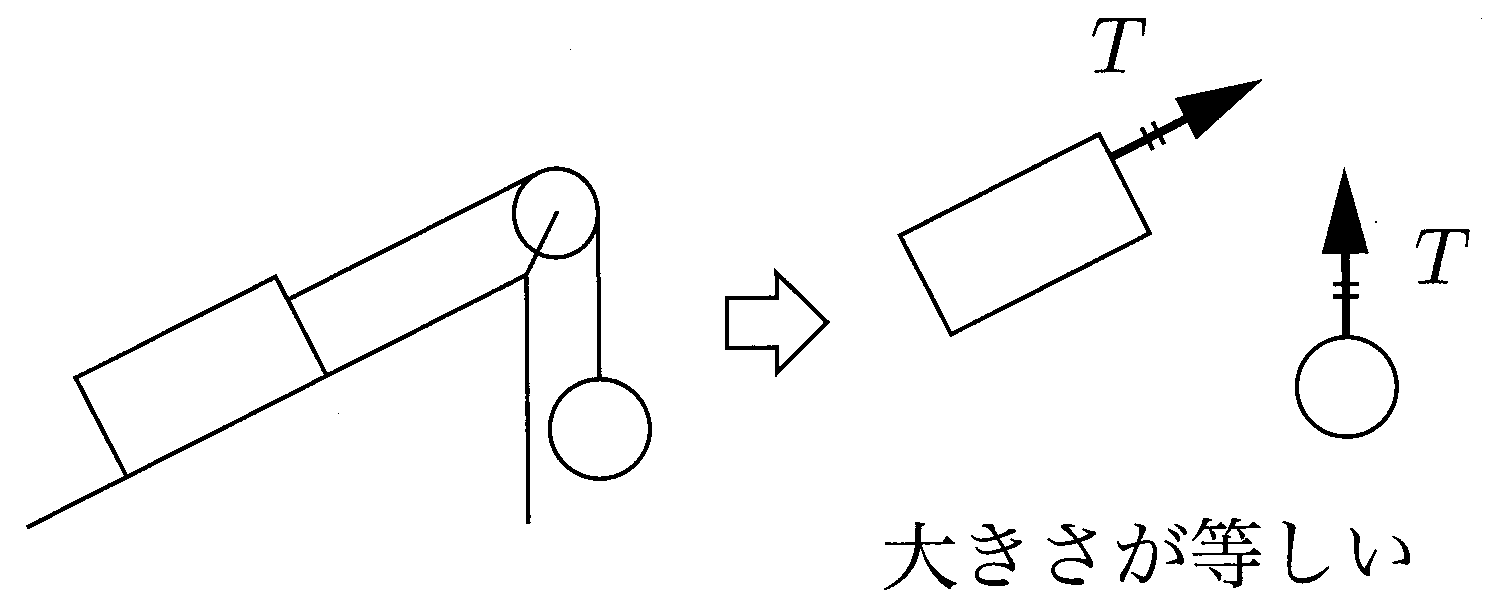
\includegraphics[keepaspectratio,width=60mm]
  {text_p16_fig3.png}
\end{wrapfigure}

糸がぴんと張っているとき，糸には張力が作用し，向きは糸が張っている方向となる．
質量が無視できる場合，その力の大きさはどこでも同じ大きさになる．
垂直抗力の場合と同様に，
{\bf 大きさは未知量として扱い，力のつり合いや運動方程式をもとに計算する．}

糸がぴんと張っている条件は，力のつり合いの式や運動方程式によって計算して求められた張力の大きさが実際に存在する，つまり張力の大きさを$T$[N]とすれば$T\geqq 0$となることである．\vspace{10mm}

\fbox{4} 浮力

\begin{wrapfigure}[5]{r}[5mm]{30mm}
  \centering
  \vspace{-8mm}
  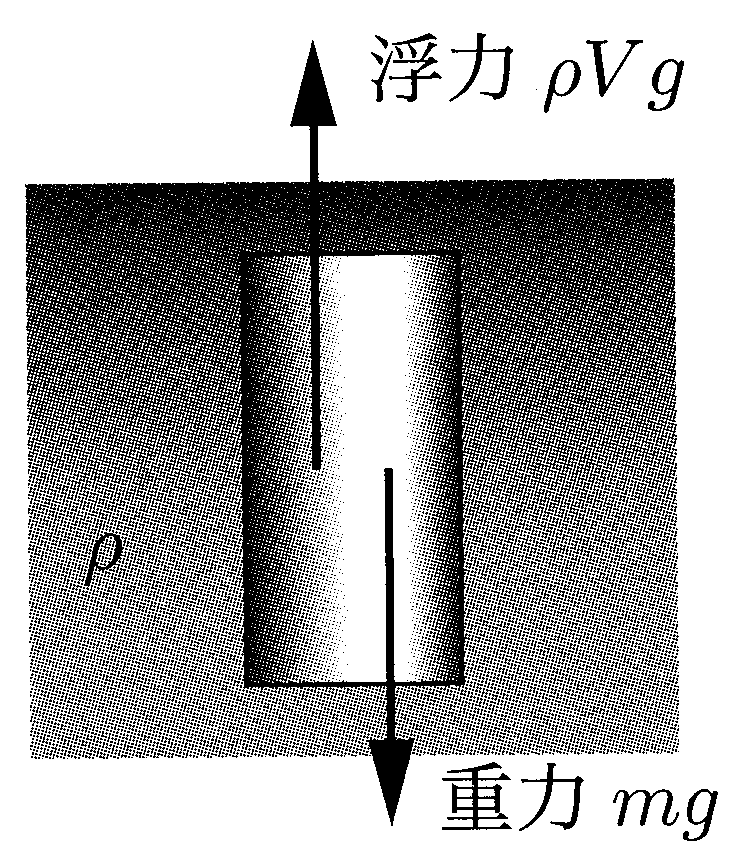
\includegraphics[keepaspectratio,width=30mm]
  {text_p16_fig4.png}
\end{wrapfigure}

物質が液体（または気体）中にあるとき，物質は物質が押しのけた液体（または気体）が本来受けていた重力と同じ大きさの浮力を鉛直上向きに受ける．
密度$\rho [{\rm kg/m^3}]$の液体中にすべて浸かっている体積$V[{\rm m^3}]$の物体は鉛直上向きに$\rho Vg$[N]の力を受ける．


%\newpage
 

%\begin{breakbox}
%\ex＜力のつり合い＞\\
%\begin{wrapfigure}[5]{r}[5mm]{45mm}
%  \centering
%  \vspace{-5mm}
%  \includegraphics[keepaspectratio,width=35mm]
%  {text_p17_fig1.png}
%\end{wrapfigure}
%\hspace{5mm}天井からつるした糸Iに質量$m$[kg]のおもりをつるし，これに糸IIをつけて水平方向に引っ張ったところ，糸Iが鉛直線と$30^\circ$の角をなしておもりがつり合った．
%このときの糸I，IIの張力の大きさを求めよ．
%ただし，重力加速度の大きさを$g {\rm [m/s^2]}$とする．\vspace{15mm}
%\end{breakbox}

力学の問題はまず{\bf 力の作用図を作図する}ことが第一歩である．
作用する力を書き出し，静止している物体にかかっている力のつり合いを考える．\\

% 
%\begin{breakbox}
%\ex＜斜面上の力のつり合い＞\\
%\begin{wrapfigure}[5]{r}[5mm]{60mm}
%  \centering
%  \vspace{-5mm}
%  \includegraphics[keepaspectratio,width=50mm]
%  {text_p17_fig2.png}
%\end{wrapfigure}
%\hspace{5mm}質量$m_1$[kg]の物体Aと，質量$m_2$[kg]の物体Bを糸で連結し，水平面上に固定された傾斜角$\theta$のなめらかな斜面に図のようにおき，そっと手を離したところAとBはそのまま静止し続けたという．
%このとき，糸の張力の大きさ$T$[N]，物体Aに作用する垂直抗力の大きさ$N$[N]を$m_1,g,\theta$で表し，$m_2$を$\theta$で表せ．
%ただし，重力加速度の大きさを$g {\rm [m/s^2]}$とする．
%\end{breakbox}

斜面上に置かれた物体の力のつり合いを考える場合には，斜面に平行な方向と垂直な方向とに成分分解してつり合いを考えると，分解する力が少なく，力のつり合いを立式しやすい．
 \ 
\newpage
\subsection{弾性力}

\fbox{5} 弾性力

\begin{wrapfigure}[12]{r}[5mm]{60mm}
  \centering
  \vspace{-5mm}
  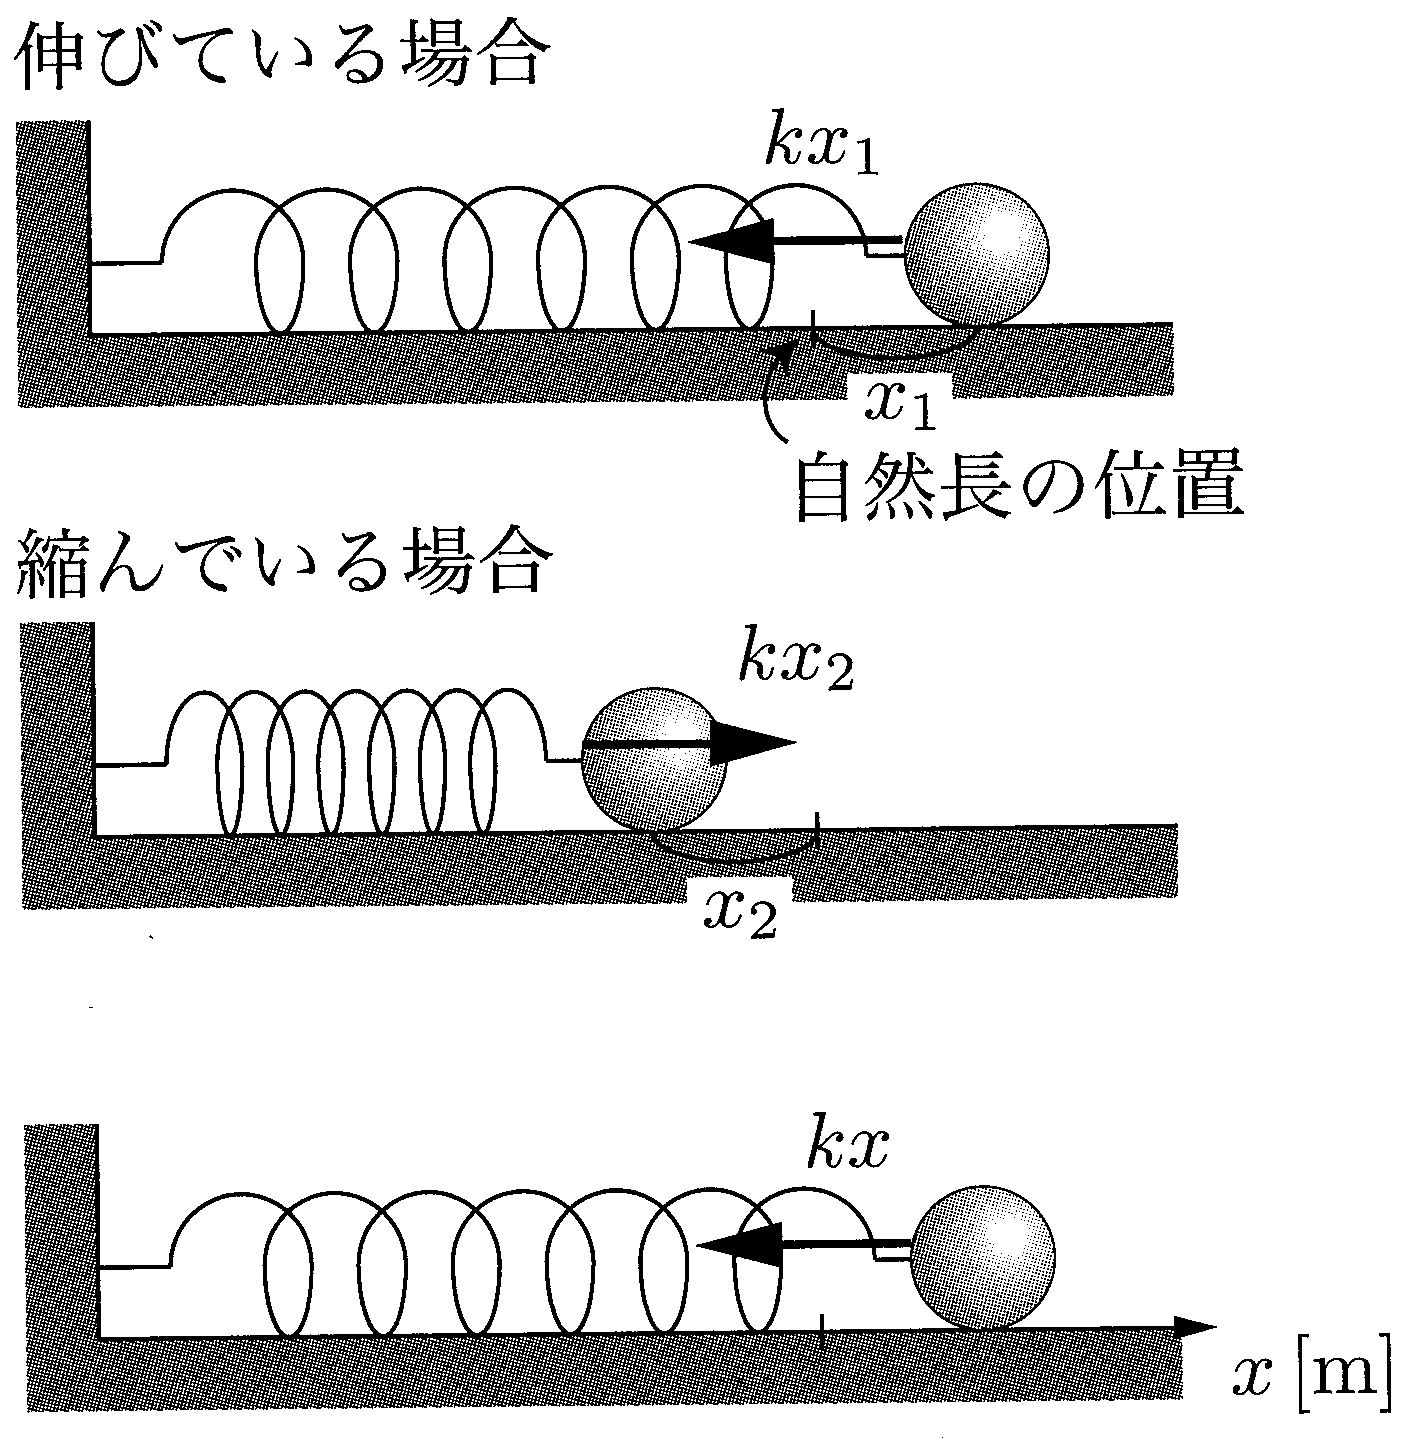
\includegraphics[keepaspectratio,width=60mm]
  {text_p18_fig1.png}
\end{wrapfigure}

バネが伸びたり縮んだりすると，バネの長さをもとの長さ（{\bf 自然長}）に戻す方向に伸び縮みの大きさに比例した力を受ける（フックの法則）．
この比例定数を{\bf バネ定数}，または{\bf 弾性定数}という．
バネ定数$k$[N/m]のバネが自然長から$x_1$[m]伸びている場合には縮める方向に$kx_1$[N]の力が，自然長から$x_2$[m]縮んでいる場合には伸びる方向に$kx_2$[N]の力が作用する．

これらをまとめて表すと，伸びる方向を正として自然長からの変位を$x$[m]（縮んでいる場合は$x$は負の値となる）とすれば，$x$軸方向の弾性力は
\[ F=-kx\]
となる（符号に注意）．

\begin{matome}{弾性力}
 
 $\hspace{5mm}自然長位置を原点とし，変位をx$[m]とするとき，バネは物体を自然長の位置に引き戻す方向に\\大きさ$kx$[N]の力を作用する．向きを含めて，
 \[F=-kx\]
 \end{matome}

% \ 
% 
%\begin{breakbox}
%\ex＜弾性力＞\\
%
%ばね定数$k$[N/m]．自然長$l$[m]のばねを天井からつりさげ，その下端に質量$m$[kg]の物体を取り付けたところ，ばねはある長さだけ伸びてつり合って静止したという．
%このときのばねの伸びを求めよ．
%ただし，重力加速度の大きさを$g {\rm [m/s^2]}$とする．
%\end{breakbox}

%\newpage
\subsection{静止摩擦力}

\fbox{6} 静止摩擦力

\begin{wrapfigure}[5]{r}[5mm]{40mm}
  \centering
  \vspace{-5mm}
  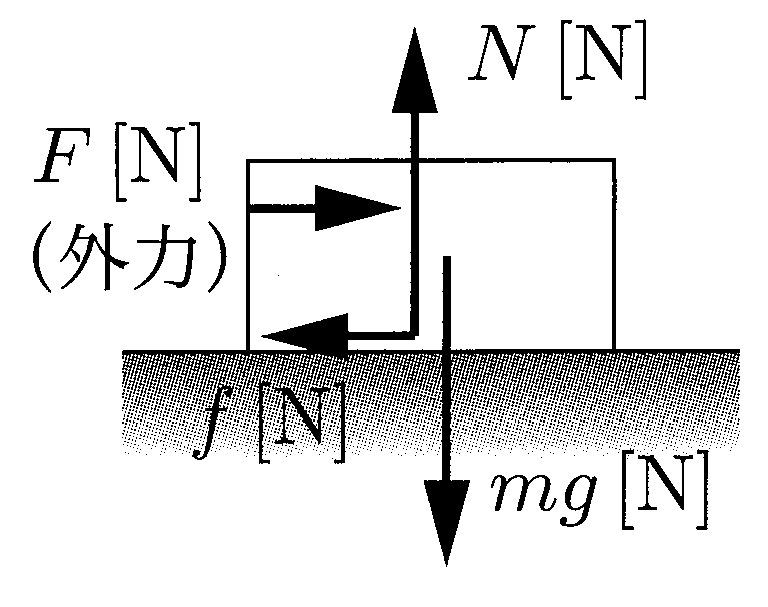
\includegraphics[keepaspectratio,width=40mm]
  {text_p19_fig1.png}
\end{wrapfigure}

粗い水平面の上に質量$m$[kg]の物体を置き，水平に外力$F$[N]を加える場合を考える．
このとき，粗い面の上であれば外力が大きくならないと滑り出さない．
滑り出すまでの間，物体は静止しているので，物体に働いている力はつり合っているが，このとき滑り出すのを妨げている力のことを{\bf 静止摩擦力}という．
静止摩擦力は接触面と平行な方向に作用し，$fやR$などの文字を利用して表すが，{\bf その大きさは未知であり，つり合いの式もしくは運動方程式から求める．}

一般に，{\bf 粗い面＝摩擦のある面，なめらかな面＝摩擦がない面}を意味する．

静止摩擦力は力のつり合いの式（もしくは運動方程式）を満たす大きさをとるが，その大きさには上限値がある．
静止摩擦力がこの上限値を超えると，もはや摩擦によって物体を静止させておくことができなくなり，物体は滑り出す．
静止摩擦力のとりうる上限値のことを{\bf 最大静止摩擦力}という．
すなわち，{\bf 静止するために必要な静止摩擦力が最大静止摩擦力を超えると物体は滑り出す．}

最大静止摩擦力の大きさは，接触面に作用する垂直抗力の大きさ$N$[N]に比例し，$\mu_0N$で与えられる．
この比例定数$\mu_0$を{\bf 静止摩擦係数}という．
静止摩擦係数は2つの物体の素材や形によって決まる定数である．

接触面の間に作用する力はこの摩擦力と垂直抗力の2つであり，この2つの力の合力を{\bf 抗力}という．
\mbox{\boldmath $静止摩擦力の大きさは最大静止摩擦力\mu_0Nであるとは限らない．$}
力のつり合いの式から計算する．

\begin{matome}{静止摩擦力}
 \hspace{5mm} 粗い面において摩擦力が作用する．\\
 \hspace{5mm} 静止摩擦力の大きさは未知数として扱い，力のつり合いまたは運動方程式から求める．
 \end{matome}

 \ 
 
%\begin{breakbox}
%\ex＜静止摩擦力＞\\
%\begin{wrapfigure}[3]{r}[5mm]{60mm}
%  \centering
%  \vspace{-5mm}
%  \includegraphics[keepaspectratio,width=50mm]
%  {text_p19_fig2.png}
%\end{wrapfigure}
%\hspace{5mm}質量$m$[kg] の物体Aを粗い板の上に乗せ，板をゆっくりと傾けて板が水平面と角度$\theta$をなすようにしたところ，物体は静止し続けたという．
%重力加速度の大きさを$g [{\rm m/s^2}]$とし，Aと板の間の静止摩擦係数を$\mu_0$とする．以下の問いに答えよ．
%\begin{description}
%\item[(1)] Aに作用する垂直抗力の大きさ$N$[N]，Aに作用する静止摩擦力の大きさ$f$[N]を求めよ．
%\item[(2)] 板をゆっくりとさらに傾けていくと，傾斜角が$\theta_0$となったところで物体は滑り始めた．角度$\theta_0$の満たす式を求めよ．
%\end{description}
%
%\end{breakbox}
%
\newpage
\subsection{作用・反作用の法則}

力は決して一方的に作用することはなく，$AがBに力（作用）を及ぼすと，BはAに対して逆向き・同じ大きさの力（反作用）を及ぼし返す．$これを{\bf 作用・反作用の法則}（運動の第三法則）という．
力の作用図を書き出すときは，どの物体にかかる力なのかを意識すること．

\begin{matome}{作用・反作用の法則}
 \hspace{5mm} 物体Aが物体Bに力を及ぼすとき，物体Aは物体Bから等大逆向きの力を受ける．
 \end{matome}

 \ 
% 
%\begin{breakbox}
%\ex＜作用・反作用の法則と力の作図＞\\
%\begin{wrapfigure}[5]{r}[5mm]{60mm}
%  \centering
%  \vspace{-5mm}
%  \includegraphics[keepaspectratio,width=50mm]
%  {text_p20_fig1.png}
%\end{wrapfigure}
%\hspace{5mm}なめらかな水平面Cの上に，質量$M$[kg]の箱型の物体Bが，さらにその上に質量$m$[kg]の箱型の物体Aが乗せられて静止している．
%重力加速度の大きさを$g [{\rm m/s^2}]$として以下の問いに答えよ．
%\begin{description}
%\item[(1)] この系に作用するすべての力を書き出せ．AとBの間に作用する垂直抗力の大きさを$N_1$[N]とし，Bと床Cの間に作用する垂直抗力の大きさを$N_2$[N]とせよ．
%\item[(2)] $N_1,N_2$を求めよ．
%\end{description}
%
%\end{breakbox}

%%%%%%%%%%%%%%%%%%%%  練習問題（旧 prob_p8.png〜prob_p10.png）  %%%%%%%%%%%%%%%%%%%%
\newpage
\Rank{A問題}

\Mon{基本事項の確認}

\hspace{1zw}下図において，球体は静止している．また，(3)において，球体と斜面との間の摩擦は無視してよい．このとき，球体に作用している力を作図し，各々の力を「○○が△△に及ぼす××力」という形で答えよ（各々の力の大きさは求めなくてよい）．
\begin{center}
\begin{minipage}[t]{0.27\linewidth}
(1)\par\centering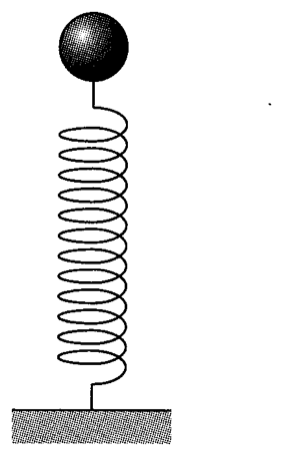
\includegraphics[keepaspectratio,width=20mm]{fig/ch3_p8_19a.png}
\end{minipage}\hfill
\begin{minipage}[t]{0.22\linewidth}
(2)\par\centering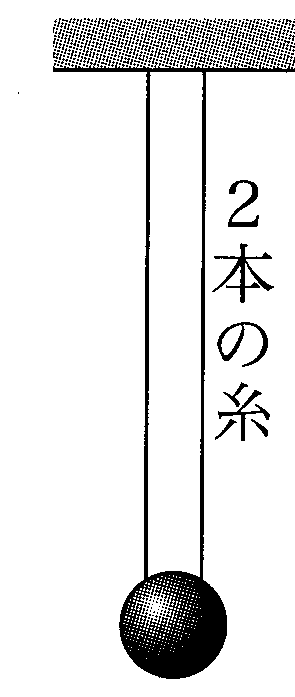
\includegraphics[keepaspectratio,width=14mm]{fig/ch3_p8_19b.png}
\end{minipage}\hfill
\begin{minipage}[t]{0.38\linewidth}
(3)\par\centering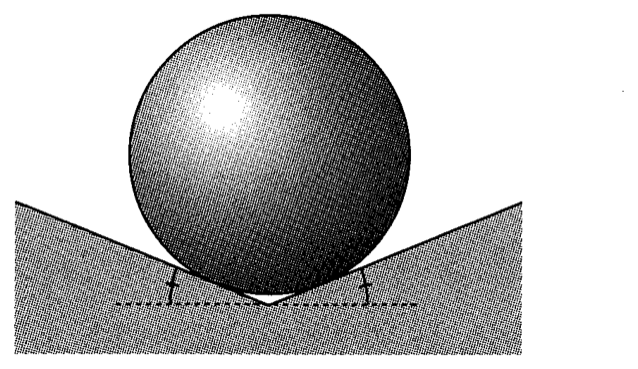
\includegraphics[keepaspectratio,width=45mm]{fig/ch3_p8_19c.png}
\end{minipage}
\end{center}

\Mon{基本事項の確認}

\begin{zuright}{43mm}
\hspace{1zw}机の上に板$\mathrm{B}$を置き，その上に物体$\mathrm{A}$を乗せる．次の力のうちで，
\begin{komon}
\ko{1} つり合いの関係にある力の組み合わせをすべて挙げよ．
\ko{2} 互いに作用・反作用の関係にある力の組み合わせをすべて挙げよ．
\end{komon}
\zusep
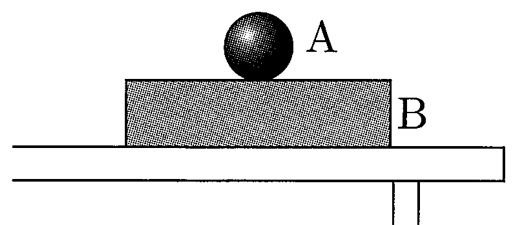
\includegraphics[keepaspectratio,width=36.5mm]{fig/ch3_p8_20.png}
\end{zuright}
\noindent\begin{tabular}{@{}p{0.49\linewidth}@{}p{0.49\linewidth}@{}}
\MARU{1}\quad 板$\mathrm{B}$が物体$\mathrm{A}$を押す力 &
\MARU{2}\quad 物体$\mathrm{A}$が板$\mathrm{B}$を押す力 \\
\MARU{3}\quad 板$\mathrm{B}$が机を押す力 &
\MARU{4}\quad 地球が物体$\mathrm{A}$を引く力 \\
\MARU{5}\quad 机が板$\mathrm{B}$を押す力 &
\MARU{6}\quad 地球が板$\mathrm{B}$を引く力 \\
\MARU{7}\quad 机が物体$\mathrm{A}$を押す力 &
\end{tabular}

\Rank{B問題}

\Mon{力のつり合い}

\begin{zuright}{62mm}
\hspace{1zw}右図のように，天井の2点$\mathrm{A}$，$\mathrm{B}$から糸$\mathrm{AC}$，$\mathrm{BC}$をぶら下げて質量$m\U{kg}$の物体をつり下げたところ，鉛直方向とそれぞれ$45^\circ$，$60^\circ$の角をなしてつり合った．このとき糸$\mathrm{AC}$，$\mathrm{BC}$の張力の大きさ$T_1$，$T_2$を求めよ．ただし，重力加速度の大きさを$g\U{m/s^2}$とする．
\zusep
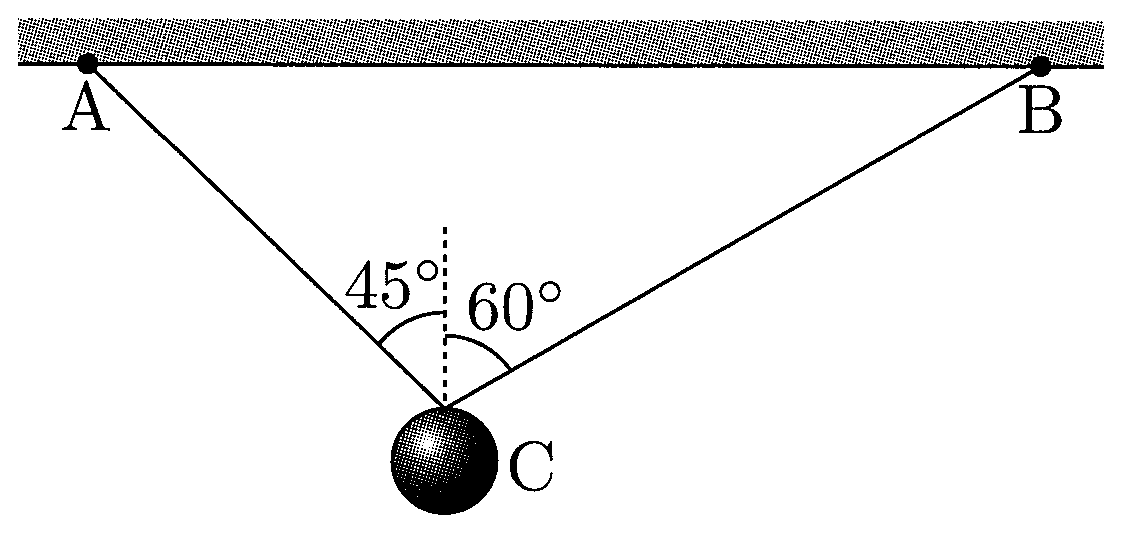
\includegraphics[keepaspectratio,width=51mm]{fig/ch3_p8_21.png}
\end{zuright}

\Mon{弾性力}\Sitei

\begin{zuright}{22mm}
\hspace{1zw}右図のように，質量が$m_1\U{kg}$のおもり$\mathrm{A}$と，質量が$m_2\U{kg}$のおもり$\mathrm{B}$を軽い糸と弾性定数$k\U{N/m}$の軽いばねでつるしたところ，ばねがある長さだけ伸びて各物体はつり合って静止した．重力加速度の大きさを$g\U{m/s^2}$として，以下の問いに答えよ．
\begin{komon}
\ko{1} 糸の張力の大きさを求めよ．
\ko{2} ばねの伸びを求めよ．
\end{komon}
\zusep
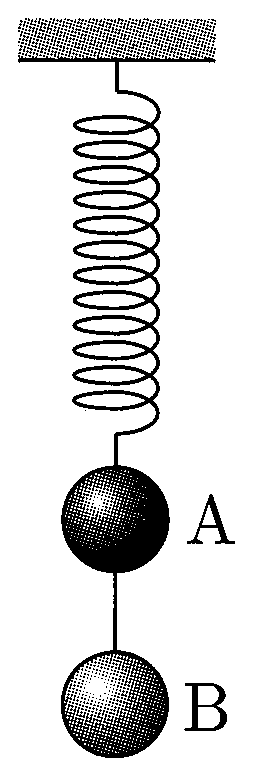
\includegraphics[keepaspectratio,width=12mm]{fig/ch3_p8_22.png}
\end{zuright}

\Mon{斜面上での最大摩擦力}

\begin{zuright}{52mm}
\hspace{1zw}右図のように，粗い面を持つ水平な板の上に質量$2.0\U{kg}$の物体を置き，水平方向に外力を加えたところ，外力が$8.0\U{N}$を越えると物体は板の上をすべり出した．重力加速度の大きさを$9.8\U{m/s^2}$として，以下の問いに有効数字2桁で答えよ．
\begin{komon}
\ko{1} 物体と板の間の静止摩擦係数を求めよ．
\ko{2} 板の上にこの物体を置いて，板を静かに傾けていく．物体がすべり始めるときの板の傾きを$\theta\U{rad}$とするとき，$\tan\theta$の値を求めよ．
\end{komon}
\zusep
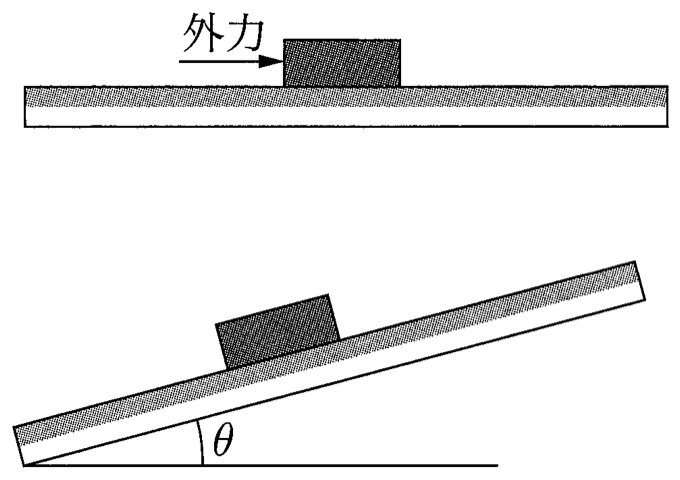
\includegraphics[keepaspectratio,width=48mm]{fig/ch3_p9_23.png}
\end{zuright}

\Mon{作用・反作用}

\begin{zuright}{35mm}
\hspace{1zw}次の文の空欄を適当な語句で埋めよ．

\hspace{1zw}台ばかりに物体$\mathrm{P}$をのせて質量を計ることができるのはなぜかを考えてみよう．重力加速度の大きさを$g\U{m/s^2}$，物体$\mathrm{P}$の質量を$m\U{kg}$とする．\MARU{3}\MARU{6}\MARU{7}は式で，その他は言葉で答えよ．

\hspace{1zw}物体$\mathrm{P}$には重力と\fbox{\MARU{1}}が作用しているが，物体$\mathrm{P}$が静止しているときにはこの二つの力は\fbox{\MARU{2}}の関係にあるので，\fbox{\MARU{1}}の大きさは\fbox{\MARU{3}}になる．

\hspace{1zw}さて，台ばかりの内部は図のように鉛直に取り付けられたバネの上に皿が乗っている構造になっており，前面の針はバネの縮みに応じて回転する仕組みになっている．台ばかりの皿は軽く，その質量を無視してよいものとして，皿に作用する力を考えると，皿にはバネからの弾性力と，\fbox{\MARU{1}}の\fbox{\MARU{4}}の関係にある力である\fbox{\MARU{5}}が作用する．そのため，この力によってバネは押し縮められる．弾性定数を$k\U{N/m}$，バネの縮みを$x\U{m}$とすると，皿に作用する力のつり合いの式は\fbox{\MARU{6}}となり，これからバネの縮みは\fbox{\MARU{7}}となる．よって，台ばかりの内部のバネの縮みの距離から，皿の上に乗っている物体の質量$m\U{kg}$を逆算することができる．
\zusep
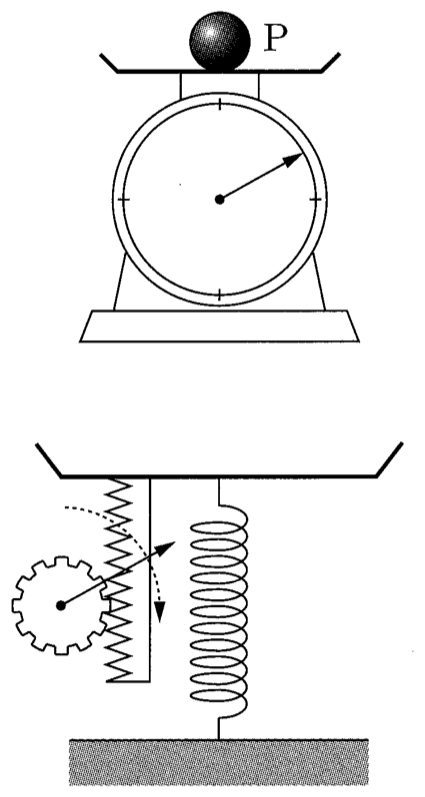
\includegraphics[keepaspectratio,width=30mm]{fig/ch3_p9_24.png}
\end{zuright}

\Mon{力のつり合い}\Sitei

\begin{zuright}{47mm}
\hspace{1zw}右図のように，仰角$30^\circ$のなめらかな斜面上に，天井から糸でつるした質量$m\U{kg}$の物体を置いたところ，糸が鉛直方向と$30^\circ$の角をなしてつり合った．糸の張力と，斜面から物体に作用する垂直抗力の大きさを求めよ．ただし，重力加速度の大きさを$g\U{m/s^2}$とする．
\zusep
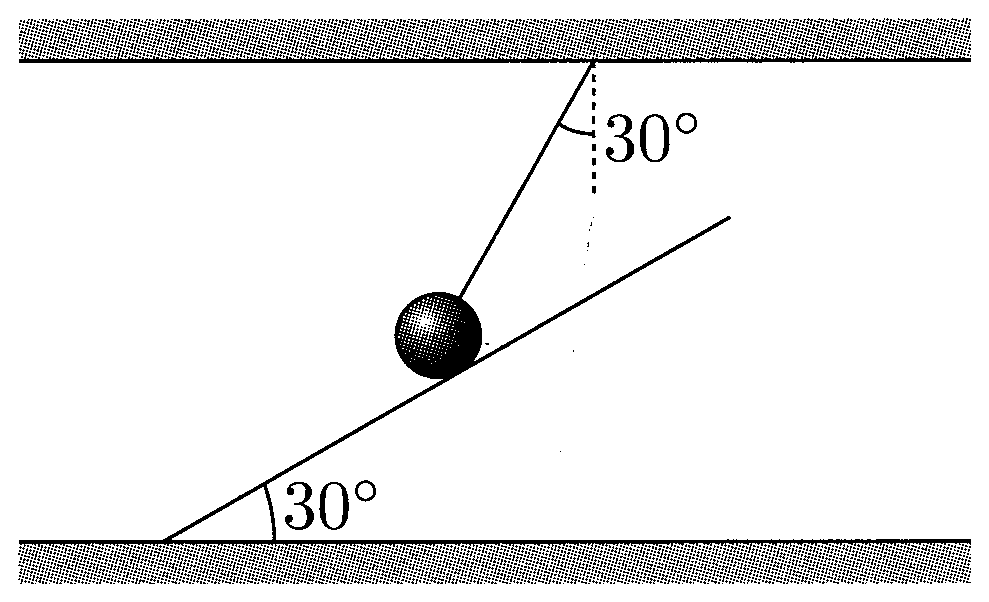
\includegraphics[keepaspectratio,width=47mm]{fig/ch3_p9_25.png}
\end{zuright}

\filbreak
\Rank{C問題}

\begingroup
\let\filbreak\relax
\Mon{弾性力}
\endgroup

\begin{zuright}{47mm}
\hspace{1zw}右図のように，自然長が$l\U{m}$でばね定数の等しいばね2本を，距離$2l\U{m}$だけ離して天井にとりつけ，2つのばねの下端をつないだ．2つのばねの先に，質量$m\U{kg}$のおもり$\mathrm{A}$をつないだところ，ばねは鉛直線と$45^\circ$の角をなしてつり合った．次に，質量$M\U{kg}$のおもり$\mathrm{B}$をつないだところ，ばねは鉛直線と$30^\circ$の角をなしてつり合った．$\mathrm{A}$と$\mathrm{B}$のおもりの質量の比$\dfrac{m}{M}$を求めよ．
\zusep
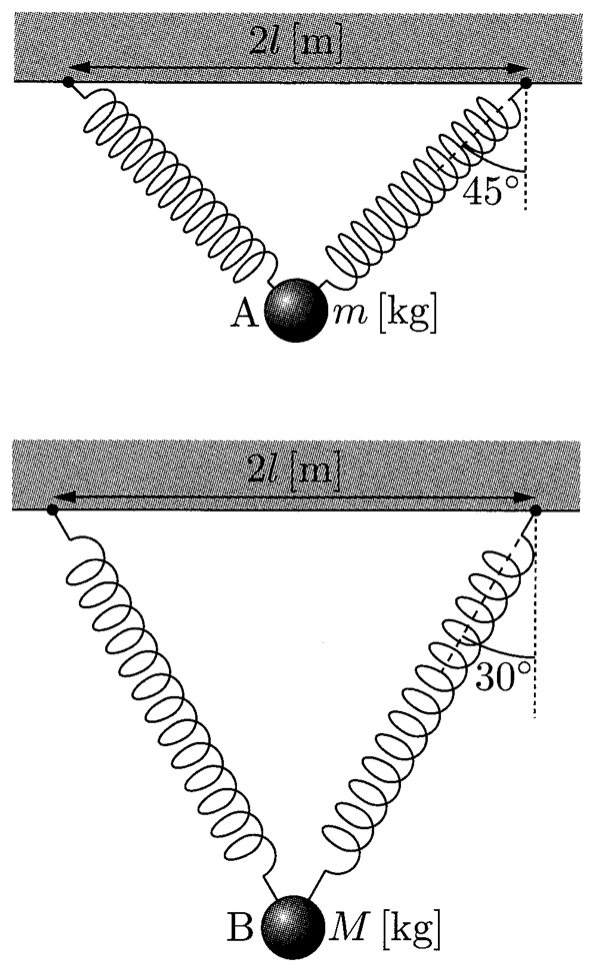
\includegraphics[keepaspectratio,width=42mm]{fig/ch3_p10_26.png}
\end{zuright}

\Mon{斜面上での最大摩擦力}

\begin{zuright}{47mm}
\hspace{1zw}右図のように，摩擦のある平板上に質量$m\U{kg}$の小物体が置かれている．重力加速度の大きさを$g\U{m/s^2}$として以下の問いに答えよ．
\begin{komon}
\ko{1} 板を静かに傾けていくと，板が水平面と角$\alpha_0$をなしたときに物体は滑り始めた．このことから，板と物体の間の静止摩擦係数$\mu_0$を$\alpha_0$で表せ．
\ko{2} 傾斜角を増して$\alpha\ (\alpha>\alpha_0)$にするとき物体が滑るのを防ぐためには，板面に平行上向きにどれだけの力を加えればよいか．その最小の力を求めよ．
\end{komon}
\zusep
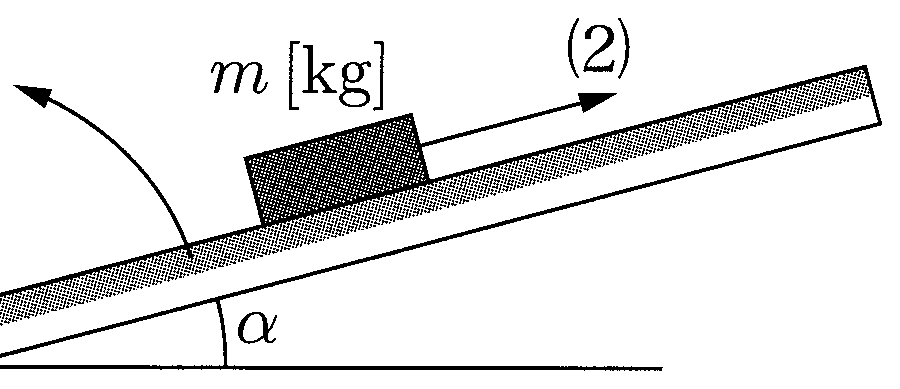
\includegraphics[keepaspectratio,width=42mm]{fig/ch3_p10_27.png}
\end{zuright}

\newpage
%%%%%%%%%%%%%%%%%%%%  解答（旧 prob_p72_2.png〜prob_p76_1.png）  %%%%%%%%%%%%%%%%%%%%
\KaiTitle{第3回　物体に作用する力とつり合い}
\setlength{\columnseprule}{0.4pt}
\begin{multicols}{2}
\raggedcolumns


\Rank{A問題}
\MonN{19}{基本事項の確認}\par\nopagebreak
\begin{sisin}
\hspace{1zw}物体に作用する力は，場の力，接触力，作用・反作用の順番に考えていくとよい．なお，場の力である重力は，地球が物体を引く力であるから作用主は地球である．
\end{sisin}
\KaiHead
\begin{zuright}{24mm}
\begin{komon}
\ko{1} 重力$W$\\
ばねが物体に及ぼす弾性力$F$
\end{komon}
\zusep
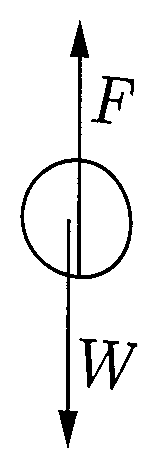
\includegraphics[keepaspectratio,height=26mm]{fig/ch3_p72_19a.png}
\end{zuright}
\begin{zuright}{28mm}
\begin{komon}
\ko{2} 重力$W$\\
右の糸が物体に及ぼす張力$T_1$\\
左の糸が物体に及ぼす張力$T_2$
\end{komon}
\zusep
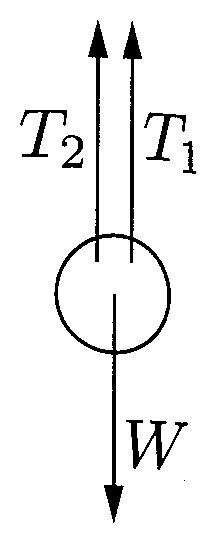
\includegraphics[keepaspectratio,height=30mm]{fig/ch3_p72_19b.png}
\end{zuright}
\begin{zuright}{32mm}
\begin{komon}
\ko{3} 重力$W$\\
右の斜面が物体に及ぼす垂直抗力$N_1$\\
左の斜面が物体に及ぼす垂直抗力$N_2$
\end{komon}
\zusep
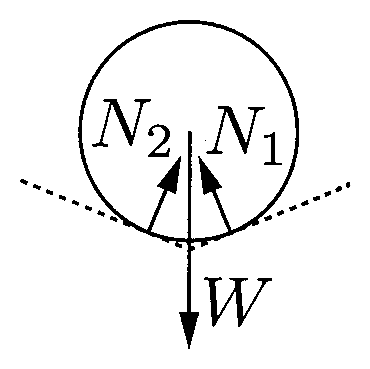
\includegraphics[keepaspectratio,width=28mm]{fig/ch3_p72_19c.png}
\end{zuright}

\MonN{20}{基本事項の確認}\par\nopagebreak
\begin{sisin}
\hspace{1zw}力のつり合いと，作用・反作用の関係とは異なるものであることに注意せよ．力のつり合いとは，\underline{ある一つ}\hskip0pt\underline{の物体に}\hskip0pt\underline{作用する}\hskip0pt\underline{いくつか}\hskip0pt\underline{の力が}\hskip0pt\underline{互いに}\hskip0pt\underline{打ち消し}\hskip0pt\underline{合っている}ことを言い，作用・反作用の関係とは，\underline{二つの}\hskip0pt\underline{物体が}\hskip0pt\underline{互いに}\hskip0pt\underline{及ぼし}\hskip0pt\underline{合っている}\hskip0pt\underline{等大・}\hskip0pt\underline{逆向きの力}のことを言う．単純に大きさだけを見て，これが同じだからつり合いとしたり，作用・反作用であるとはしないこと．また，接触力は互いに接触していなければ作用しないので，\MARU{7}の力は存在しない．

\hspace{1zw}存在する力を「$\mathrm{A}$が$\mathrm{B}$に及ぼす○○力」と正しく言って考えると分かりやすい．つりあいの関係になるのは，「$\mathrm{B}$に」の部分が共通する複数の力である．また，作用・反作用の関係になる力は「$\mathrm{A}$が$\mathrm{B}$に」の部分が「$\mathrm{B}$が$\mathrm{A}$に」となる一組の力である．
\end{sisin}
\KaiHead
\hspace{1zw}力の作用図は次図のようになる．
\begin{center}
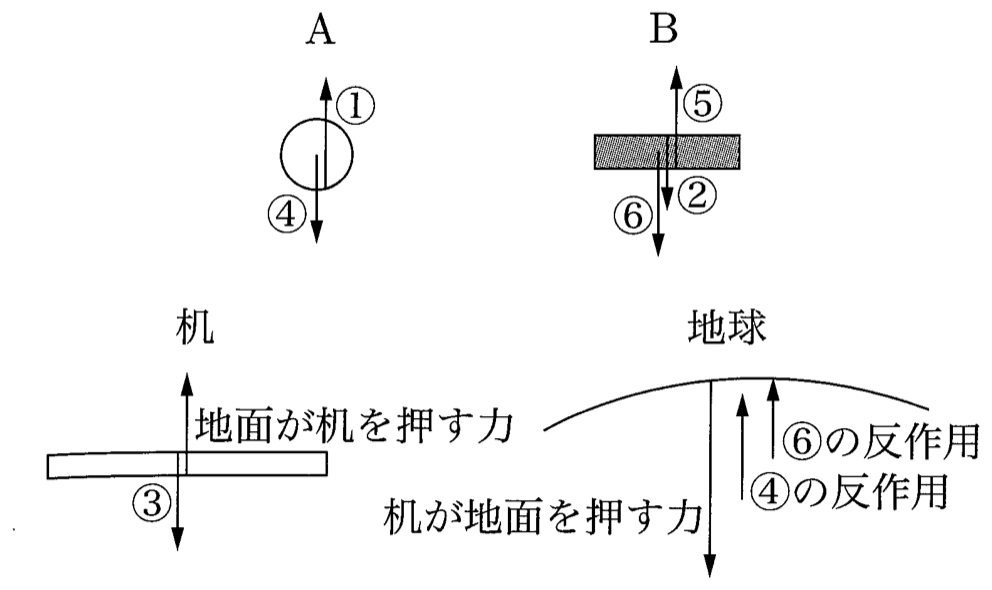
\includegraphics[keepaspectratio,width=70mm]{fig/ch3_p73_20.png}
\end{center}
\begin{komon}
\ko{1} つり合いの関係

物体$\mathrm{A}$に関して，鉛直下向きに作用する\MARU{4}と鉛直上向きに作用する\MARU{1}の力がつり合う．

板$\mathrm{B}$に関して，鉛直下向きに作用する\MARU{2}＋\MARU{6}と鉛直上向きに作用する\MARU{5}の力がつり合う．
\ko{2} 作用・反作用の関係

$\mathrm{A}$と$\mathrm{B}$間でやり取りされる垂直抗力\MARU{1}と\MARU{2}が，また$\mathrm{B}$と机間でやり取りされる垂直抗力\MARU{3}と\MARU{5}とが互いに作用・反作用の関係にある．
\end{komon}

\Rank{B問題}
\MonN{21}{力のつり合い}\par\nopagebreak
\begin{sisin}
\hspace{1zw}まず，物体に作用する力を，場の力，接触力，作用・反作用の力の順に描き出す．物体が静止している場合には描き出した力の作用図をもとにつり合い条件を考えればよい．

\hspace{1zw}力のつり合い条件のとらえ方はベクトル的に考える方法，成分分解する方法とがあるが，本問の場合は糸が2本あり，ある特殊な方向というのは考えにくい．そこで，オーソドックスに水平方向・鉛直方向に力を成分分解して，各軸方向の力のつり合いを考える．
\end{sisin}
\KaiHead
\hspace{1zw}物体に働く力の作用図は次図の通り．
\begin{center}
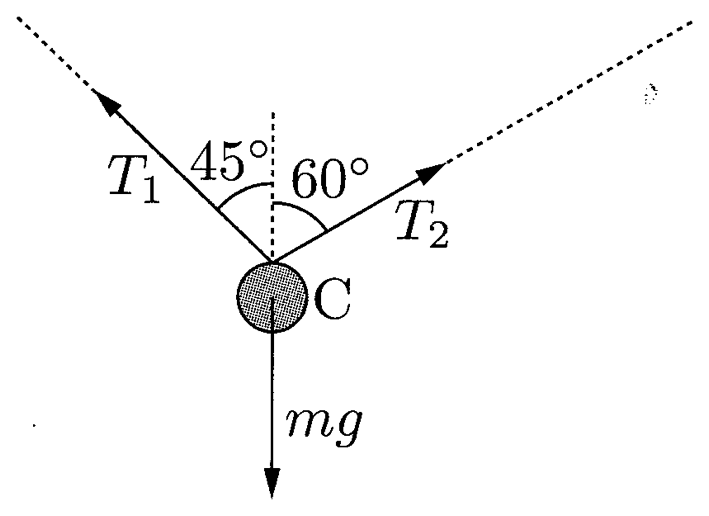
\includegraphics[keepaspectratio,width=50mm]{fig/ch3_p73_21.png}
\end{center}
\hspace{1zw}鉛直方向・水平方向のつり合いの式は，
\[
\text{鉛直方向：}\quad T_1\cos45^\circ+T_2\cos60^\circ=mg
\]
\[
\text{水平方向：}\quad T_1\sin45^\circ=T_2\sin60^\circ
\]
以上2式より，
\[
T_1=\dfrac{\sqrt2}{2}\left(3-\sqrt3\right)mg\U{N}
\]
\[
T_2=\left(\sqrt3-1\right)mg\U{N}\Ans
\]

\MonN{22}{弾性力}\par\nopagebreak
\begin{sisin}
\hspace{1zw}まず作用している力を書き出す必要がある．\underline{どの}\hskip0pt\underline{物体}\hskip0pt\underline{に対}\hskip0pt\underline{して}\hskip0pt\underline{力が}\hskip0pt\underline{作用}\hskip0pt\underline{する}\hskip0pt\underline{かに}\hskip0pt\underline{注意}\hskip0pt\underline{せよ}．物体$\mathrm{A}$については場の力として重力$m_1g$，接触力としてバネから弾性力$kx$，糸から張力$T$を受けるが，物体$\mathrm{B}$については場の力として重力$m_2g$と接触力の張力$T$の\underline{二つのみ}である．物体$\mathrm{B}$には糸しか接触しておらず，バネは接触していないから弾性力$kx$は$\mathrm{B}$には作用しない．

\hspace{1zw}同様に，各物体に対しての力のつり合いを考える際には，\underline{他の物体}\hskip0pt\underline{に作用する}\hskip0pt\underline{力を含め}\hskip0pt\underline{ては}\hskip0pt\underline{ならない}．すなわち，$\mathrm{B}$に関する力のつり合いを考えるときに$\mathrm{A}$に作用する弾性力$kx$を考えてはならないし，また$\mathrm{A}$に関する力のつり合いを考えるときに$\mathrm{B}$に作用する重力$m_2g$を含めてはならない．
\end{sisin}
\KaiHead
\begin{komon}
\ko{1} ばねののびを$x\U{m}$，糸の張力の大きさを$T\U{N}$とする．$\mathrm{A}$，$\mathrm{B}$に作用する力の作用図は次図の通りとなる．
\begin{center}
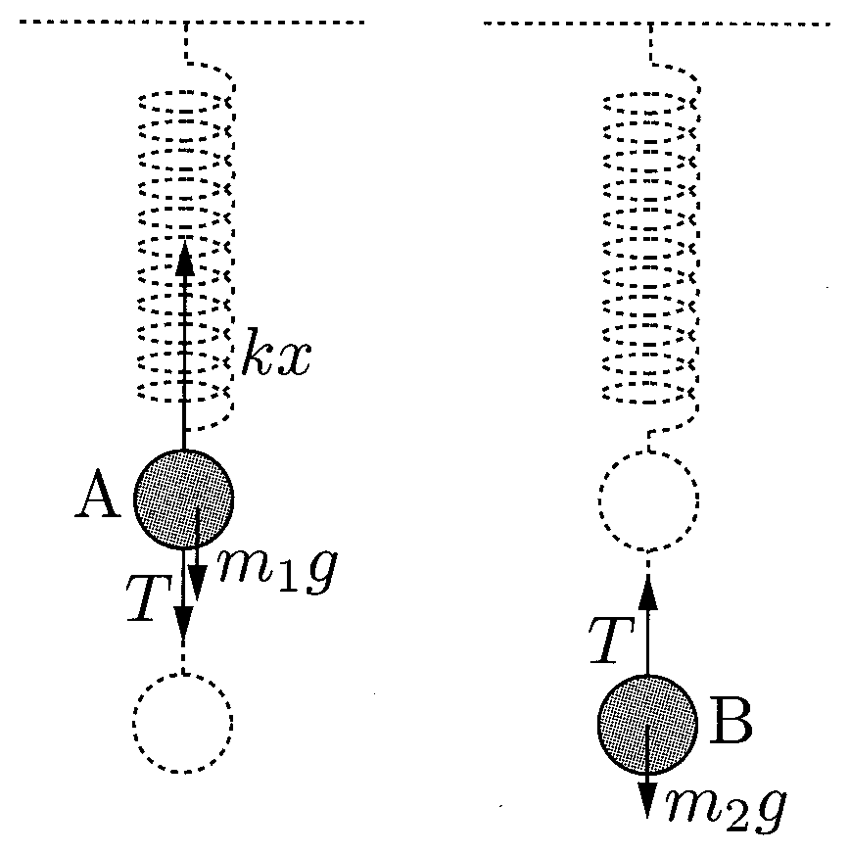
\includegraphics[keepaspectratio,width=60mm]{fig/ch3_p73_22.png}
\end{center}

よって，各物体の鉛直方向の力のつり合いの式は，
\[
\mathrm{A}:kx=m_1g+T
\]
\[
\mathrm{B}:T=m_2g
\]
以上2式より，
\[
T=m_2g\U{N}\Ans
\]
\ko{2} また，$x$については，
\[
x=\dfrac{(m_1+m_2)g}{k}\U{m}\Ans
\]
\end{komon}

\MonN{23}{斜面上での最大摩擦力}\par\nopagebreak
\begin{sisin}
\hbadness=10000
\hspace{1zw}まず，各物体に作用する力を書き出して力のつり合い条件を考えよ．\underline{静止}\hskip0pt\underline{摩擦}\hskip0pt\underline{力お}\hskip0pt\underline{よび}\hskip0pt\underline{垂直}\hskip0pt\underline{抗力}\hskip0pt\underline{の大}\hskip0pt\underline{きさ}\hskip0pt\underline{は力}\hskip0pt\underline{のつ}\hskip0pt\underline{り合}\hskip0pt\underline{いの}\hskip0pt\underline{条件}\hskip0pt\underline{式か}\hskip0pt\underline{ら決}\hskip0pt\underline{まる}ことに注意．静止摩擦力の大きさは$\mu_0N$とは限らない．本問のように，滑り出すギリギリのときには作用する静止摩擦力は最大摩擦力$\mu_0N$となるが，最初から$\mu_0N$とはおかずに，まず静止摩擦力を$f$とおき，つり合いの条件から$f$を求めて考えること．

\hspace{1zw}また，斜面上の物体のつり合いは斜面に対して平行な方向とそれに垂直な方向に力を分解して考える．
\end{sisin}
\KaiHead
\hspace{1zw}板が物体に及ぼす垂直抗力の大きさを$N\U{N}$，静止摩擦力の大きさを$f\U{N}$とする．また物体と面との間の静止摩擦係数を$\mu_0$とする．
\begin{komon}
\ko{1} 水平方向に加える外力の大きさを$F\U{N}$とするとき，物体をつり合わせるために静止摩擦力はこの外力と逆向きに作用する．ゆえに，このとき物体に働く力の作用図は次図の通り．
\begin{center}
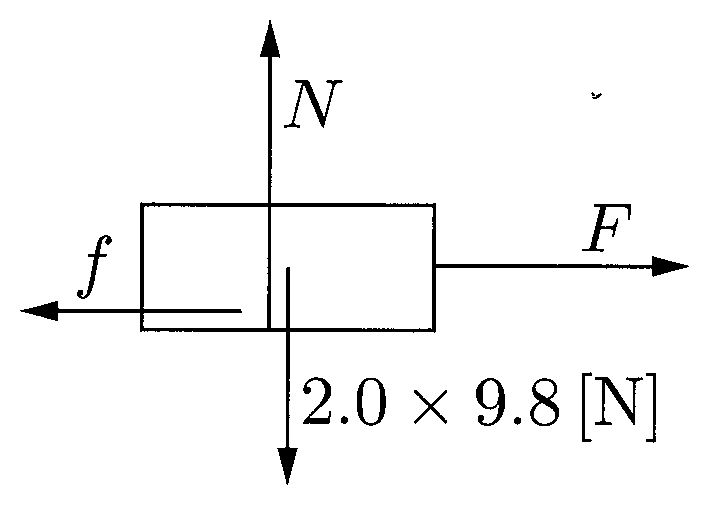
\includegraphics[keepaspectratio,width=55mm]{fig/ch3_p74_23a.png}
\end{center}

ここで，力のつり合いの条件より，
\[
\text{水平方向：}\quad f=F
\]
\[
\text{鉛直方向：}\quad N=2.0\times9.8\U{N}
\]
静止摩擦力の性質より，$f>\mu_0N=\mu_0\cdot19.6\U{N}$となると物体は滑り出すが，滑り出す瞬間の外力$F$が$8.0\U{N}$であったことから，
\[
8.0=\mu_0\cdot19.6\U{N}
\]
が成立する．よって，静止摩擦係数は
\[
\mu_0=0.408\fallingdotseq0.41\Ans
\]
\ko{2} 斜面の傾斜角が$\varphi$のときについて考える．重力の斜面方向分力$mg\sin\varphi=19.6\sin\varphi$が斜面に沿って下向きに作用して物体を滑らせようとするので，物体に作用する静止摩擦力は斜面に沿って上向きである．よって，物体に作用する力は次図の通り．
\begin{center}
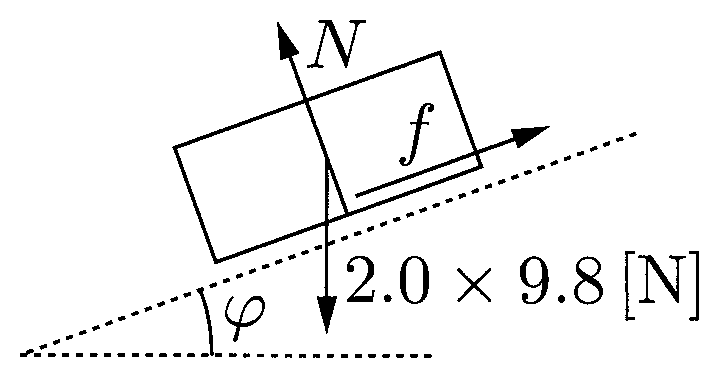
\includegraphics[keepaspectratio,width=55mm]{fig/ch3_p74_23b.png}
\end{center}

ここで，力のつり合いの条件より，
\[
\text{斜面に平行：}\quad 2\times9.8\sin\varphi=f
\]
\[
\text{斜面に垂直：}\quad N=2\times9.8\cos\varphi
\]
ゆえに，
\[
f=19.6\sin\varphi\U{N}
\]
となるが，傾斜角$\varphi$を増していくと静止しつづけるために必要な静止摩擦力は増加していき，
\[
f=\mu_0N
\]
となった直後に滑り出してしまう．その限界の角度が$\theta$であることから，
\[
19.6\sin\theta=0.408\times19.6\cos\theta
\]
整理して，
\[
\tan\theta=0.408\fallingdotseq0.41\Ans
\]
\end{komon}

\MonN{24}{作用・反作用}\par\nopagebreak
\begin{sisin}
\hspace{1zw}物体$\mathrm{P}$と台ばかりにそれぞれ着目して力の作用図を描く．うまく誘導に沿って考えよう．

\hspace{1zw}「力」についての説明を求められたら，「○○が△△に対して及ぼす××力」という形式で答えよう．何が何に対して及ぼしている力なのかを明確にすること．
\end{sisin}
\KaiHead
\hspace{1zw}物体$\mathrm{P}$および台ばかりの皿について力の作用図を描くと次図の通りとなる．
\begin{center}
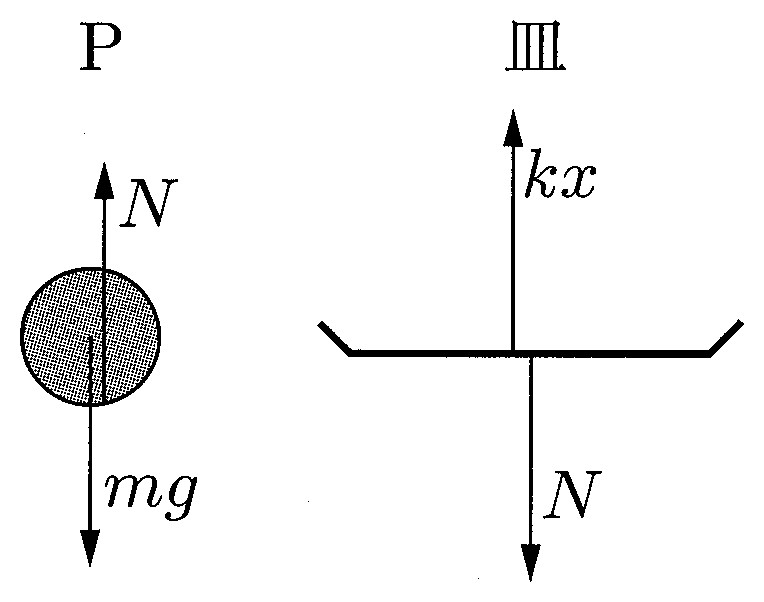
\includegraphics[keepaspectratio,width=60mm]{fig/ch3_p74_24.png}
\end{center}
\hspace{1zw}よって，
\begin{description}
\item[\MARU{1}] 皿が物体$\mathrm{P}$に及ぼす垂直抗力
\item[\MARU{2}] つり合い
\item[\MARU{3}] $mg\U{N}$
\item[\MARU{4}] 作用・反作用
\item[\MARU{5}] 物体$\mathrm{P}$が皿に及ぼす垂直抗力
\item[\MARU{6}] $kx=mg$
\item[\MARU{7}] $x=\dfrac{mg}{k}\U{m}$
\end{description}
\begin{chuu}
\hspace{1zw}\MARU{6}の立式の右辺にある$mg$は，物体$\mathrm{P}$に作用する重力ではなく，\MARU{5}の垂直抗力を表していることに注意せよ．この\MARU{5}の力は，\MARU{2}および\MARU{4}の事項より，大きさが$mg\U{N}$になっている．

% TODO: 原本では「バネばかり」表記（台ばかりの誤りと思われる）
\hspace{1zw}また，以上のことから分かるように，バネばかりは物体の質量そのものを計っているのではなく，バネばかりの皿に対して作用する力を計っている．すなわち，バネばかりの針が$m\U{kg}$を指している場合には，バネの皿に対して大きさ$mg\U{N}$の力が下向きに作用しているということを意味している．
\end{chuu}

\MonN{25}{力のつり合い}\par\nopagebreak
\begin{sisin}
\hspace{1zw}本問のような複雑な力のつり合いの問題でも，基本は\MARU{1}「作用している力の書き出し」，\MARU{2}「力のつり合いの式の立式」の二つの手順を踏むのみである．

\hspace{1zw}「なめらかな斜面」とは摩擦のない斜面のことを意味する．
\end{sisin}
\KaiHead
\hspace{1zw}糸が物体に及ぼす張力の大きさを$T\U{N}$，斜面が物体に及ぼす垂直抗力の大きさを$N\U{N}$とすれば，物体に働く力の作用図は図の通り．
\begin{center}
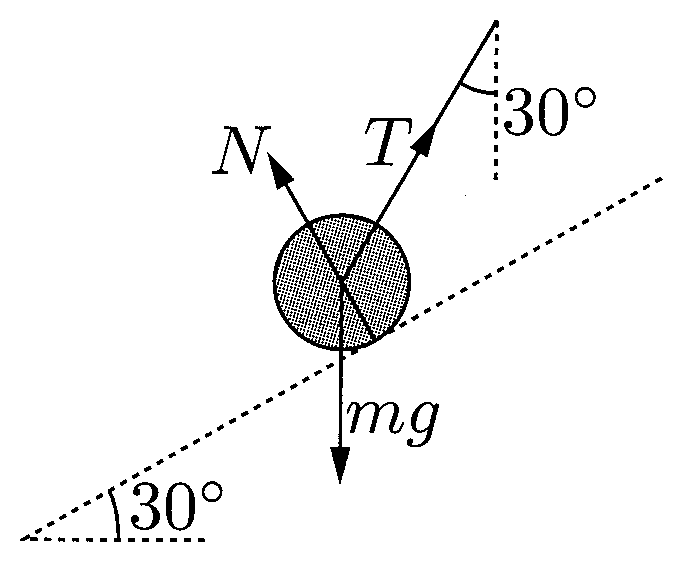
\includegraphics[keepaspectratio,width=50mm]{fig/ch3_p75_25.png}
\end{center}
\hspace{1zw}力のつり合いの式を立てると，
\[
\text{斜面に平行な方向：}\quad mg\sin30^\circ=T\cos30^\circ
\]
\[
\text{斜面に垂直な方向：}\quad N+T\sin30^\circ=mg\cos30^\circ
\]
よって，
\[
T=\dfrac{\sqrt3}{3}mg\U{N},\quad N=\dfrac{\sqrt3}{3}mg\U{N}\Ans
\]
\begin{bekkai}
\hspace{1zw}水平方向・鉛直方向に力を分解して考えてもよい．次のようになり，同じ答えが得られる．
\[
\text{水平方向：}\quad N\sin30^\circ=T\sin30^\circ
\]
\[
\text{鉛直方向：}\quad N\cos30^\circ+T\cos30^\circ=mg
\]
\end{bekkai}

\Rank{C問題}
\MonN{26}{弾性力}\par\nopagebreak
\begin{sisin}
\hspace{1zw}バネが物体に作用する力は，その伸び（もしくは縮み）によって決まる．バネの全長と伸びとを混同しないように注意せよ．
\end{sisin}
\KaiHead
\hspace{1zw}弾性定数を$k\U{N/m}$，重力加速度の大きさを$g\U{m/s^2}$とする．

\noindent\underline{物体$\mathrm{A}$について}\par
\hspace{1zw}このときのバネの全長は$\sqrt2\,l$であるから，自然長から$\left(\sqrt2-1\right)l$だけ伸びている．よって，物体$\mathrm{A}$にバネが作用する弾性力はフックの法則より$\left(\sqrt2-1\right)kl\U{N}$であり，物体$\mathrm{A}$に働く力の作用図は次図の通りとなる．
\begin{center}
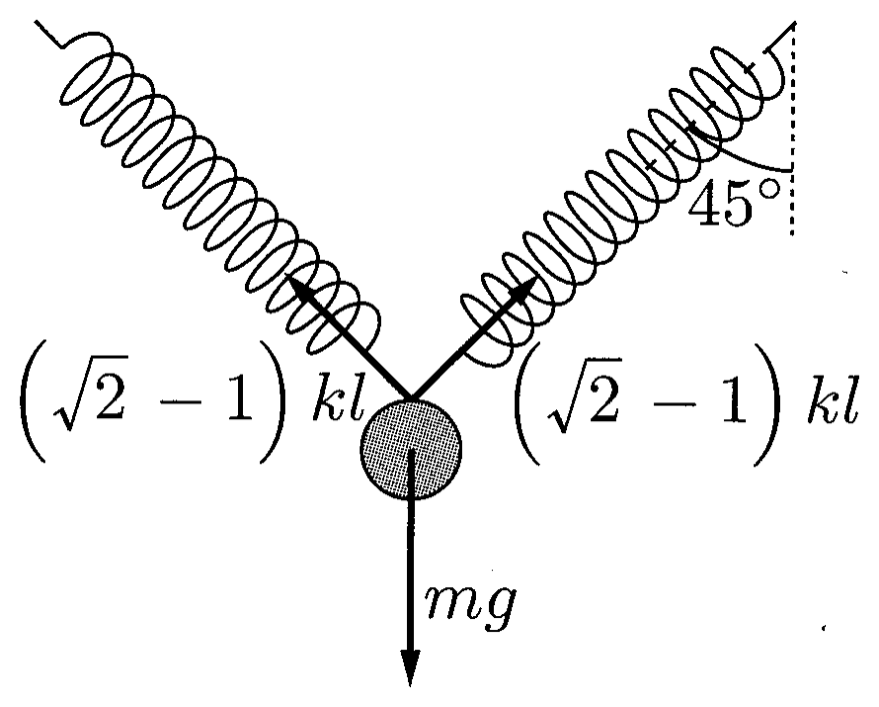
\includegraphics[keepaspectratio,width=62mm]{fig/ch3_p75_26.png}
\end{center}
\hspace{1zw}鉛直方向の力のつり合いについて，
\[
2\times\left(\sqrt2-1\right)kl\cos45^\circ=mg
\]
であるから，
\[
m=\dfrac{\left(2-\sqrt2\right)kl}{g}\U{kg}\Eq{1}
\]

\noindent\underline{物体$\mathrm{B}$について}\par
\hspace{1zw}同様に考えると，バネの全長は$2l\U{m}$なので，$\mathrm{B}$に作用する弾性力の大きさは$kl\U{N}$であり，鉛直方向の力のつり合いの式は，
\[
2\times kl\cos30^\circ=Mg
\]
よって，
\[
M=\dfrac{\sqrt3\,kl}{g}\U{kg}\Eq{2}
\]
\MARU{1}\MARU{2}より，
\[
\dfrac{m}{M}=\dfrac{2\sqrt3-\sqrt6}{3}\Ans
\]

\MonN{27}{斜面上での最大摩擦力}\par\nopagebreak
\begin{sisin}
\hspace{1zw}(1)については前出の問題と同じなのでよかろう．(2)についても基本的な考えは，力の作用図の作図，つり合いの式の立式である．問題なのは作用する静止摩擦力の向きである．この物体は重力の斜面方向分力$mg\sin\alpha$によって滑り出そうとするので，これを防ぐには静止摩擦力が上向きに作用すればよい．ところが$\alpha>\alpha_0$の場合には，物体が滑り出すのを防ぐために必要なだけの静止摩擦力を作用することができない．なるべく小さな力で物体が滑り出すのを防ぐためには，静止に必要な力を補うべく上向きに力を加えてやればよい．よって，作用している静止摩擦力は上向きと分かる．このような直観的な考え方が分かりにくい人は，静止摩擦力が下向きに作用する場合についても図を描いて立式し，考えてみよ．この場合，静止するのに必要な外力は，摩擦力が上向きに作用する場合に比べて大きくなることが計算によって示される．
\end{sisin}
\KaiHead
\hspace{1zw}物体に作用する垂直抗力の大きさを$N\U{N}$，静止摩擦力の大きさを$f\U{N}$とする．
\begin{komon}
\ko{1} 水平面との傾角が$\alpha_0$のとき，物体に働く力の作用図は次図の通り．
\begin{center}
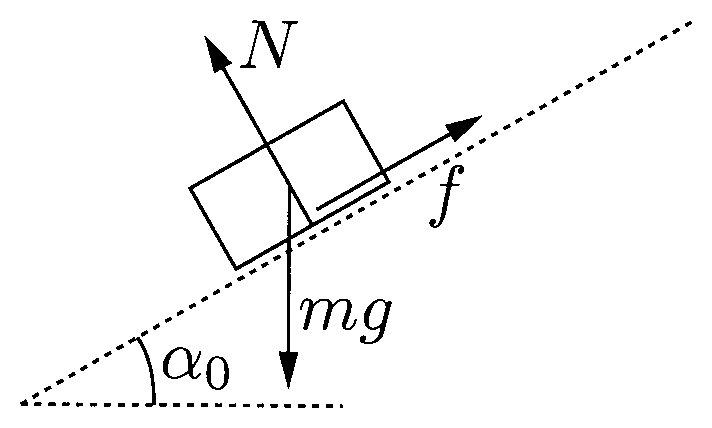
\includegraphics[keepaspectratio,width=55mm]{fig/ch3_p75_27a.png}
\end{center}

ここで，各方向の力のつり合いは，
\[
\text{斜面に平行な方向：}\quad mg\sin\alpha_0=f
\]
\[
\text{斜面に垂直な方向：}\quad N=mg\cos\alpha_0
\]
また，このとき板が物体に及ぼす静止摩擦力は最大摩擦力となっているので，
\[
f=\mu_0N
\]
以上より，
\[
\mu_0=\tan\alpha_0\Ans
\]
\ko{2} 水平面との傾角が$\alpha$のとき，物体がすべるのを防ぐために板と平行上向きに加える力の大きさを$f'$とする．このとき，物体に働く力は次図の通り．
\begin{center}
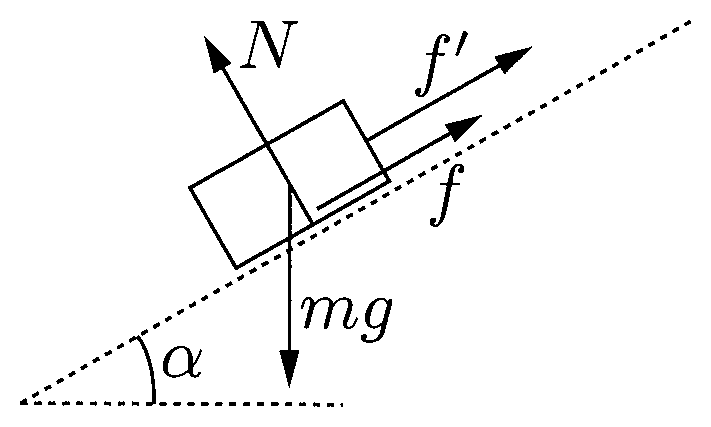
\includegraphics[keepaspectratio,width=55mm]{fig/ch3_p76_27b.png}
\end{center}

力のつり合いより，
\[
\text{斜面に平行な方向：}\quad mg\sin\alpha=f+f'
\]
% TODO: 原本ママ．「斜面に垂直な方向」の誤りと思われる
\[
\text{鉛直に垂直な方向：}\quad N=mg\cos\alpha
\]
物体が静止をしつづけるためには，作用している静止摩擦力が，最大摩擦力$\mu_0N$を越えなければよい．
\[
f\leqq\mu_0N
\]
以上の式を満たすような$f'$は，
\[
f'\geqq mg\left(\sin\alpha-\mu_0\cos\alpha\right)
\]
である．よって，加えるべき最小限の力の大きさは，これに(1)の答えを代入して
\[
mg\left(\sin\alpha-\tan\alpha_0\cos\alpha\right)\U{N}\Ans
\]
\end{komon}
\begin{bsHosoku}{参考}
\hspace{1zw}物体に加える力$f'$を大きくしていくと，いずれ物体は斜面にそって上向きに動き出す．動き始める瞬間の$f'$の大きさを求めてみよう．

\hspace{1zw}静止摩擦力の向きに注意すると，動き始める瞬間の力のつりあいの式は次のようになる．
\[
\text{斜面に平行な方向：}\quad mg\sin\alpha+f=f'
\]
% TODO: 原本ママ．「斜面に垂直な方向」の誤りと思われる
\[
\text{鉛直に垂直な方向：}\quad N=mg\cos\alpha
\]
これらと$f=\mu_0N$を連立すると，
\[
f'=mg\left(\sin\alpha+\tan\alpha_0\cos\alpha\right)
\]
が分かる．これが物体を上向きに動かすのに必要な最小の力であるから，物体を斜面上に静止させておくには，斜面にそって上向きに
\[
mg\left(\sin\alpha-\mu_0\cos\alpha\right)\leqq f'
\]
\[
\hspace{8zw}\leqq mg\left(\sin\alpha+\tan\alpha_0\cos\alpha\right)
\]
を満たす力$f'$を加えればよい．
\end{bsHosoku}

\end{multicols}

 \ 
 
\newpage
\section{運動方程式}

\subsection{運動方程式}

\begin{wrapfigure}[8]{r}[5mm]{40mm}
  \centering
  \vspace{-5mm}
  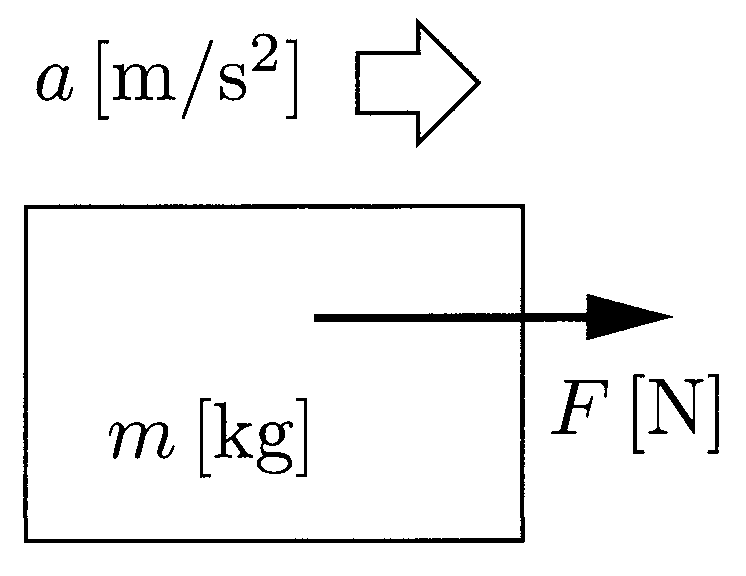
\includegraphics[keepaspectratio,width=40mm]
  {text_p21_fig1.png}
\end{wrapfigure}

物体に作用する力がつり合っているとき，物体は静止もしくは等速度直線運動を続ける．
これに対して，物体に作用する力がつり合っていないときは，物体はその力に応じた加速度を生じ，物体の運動状態が変化する．

物体の質量を$m$[kg]，物体に作用する力の合力を$F$[N]，物体の持つ加速度を$a[{\rm m/s^2}]$とすると，
\[ ma=F\]
という関係が成り立つ（運動の第二法則）．この式を{\bf 運動方程式}という．

力および加速度は一般にはベクトル量であるから，各軸方向の運動方程式を組み合わせることにより，
\[ m\overrightarrow {a}=\overrightarrow {F}\]
となる．

なお，物体に作用する全合力が$\overrightarrow {0}$，つまり$\overrightarrow {F}=\overrightarrow {0}$のときは$\overrightarrow {a}=\overrightarrow {0}$となり，{\bf 全外力がつり合っている場合は加速度が0で，等速度直線運動（もしくは静止）を行う}ことが運動方程式からも示される．

\begin{matome}{運動方程式}
 \hspace{5mm} 物体に作用している力と質量・加速度の間に$m\overrightarrow {a}=\overrightarrow {F}$が成立
 \end{matome}


 \ 
% 
%\begin{breakbox}
%\ex＜力の作図と運動方程式の立式＞\\
%\begin{wrapfigure}[7]{r}[5mm]{40mm}
%  \centering
%  \vspace{-5mm}
%  \includegraphics[keepaspectratio,width=30mm]
%  {text_p21_fig2.png}
%\end{wrapfigure}
%\hspace{5mm}定滑車に糸をかけ，その両端に質量$M$[kg]の物体Aと質量$m$[kg]の物体Bを図のようにつるす．
%Bは地上にあり，Aは高さ$h$[m]のところにある．
%物体Aを静かに離して，物体Aが落下している間の運動について以下の問いに答えよ．
%ただし，糸や定滑車の質量は無視でき，$M>m$，重力加速度の大きさを$g [{\rm m/s^2}]$とする．
%\begin{description}
%\item[(1)] 物体A，物体B，定滑車に作用するすべての力を書き出せ．
%\item[(2)] 物体Aの加速度の大きさ$a [{\rm m/s^2}]$ならびに糸の張力の大きさ$T$[N]を求めよ．
%\item[(3)] AとBがすれ違うのに要する時間$t_1$[s]およびそのときのAの速さ$v_1$[m/s]を求めよ．
%\end{description}
%
%\end{breakbox}

\subsection{動摩擦力}

\begin{wrapfigure}[8]{r}[5mm]{40mm}
  \centering
  \vspace{-5mm}
  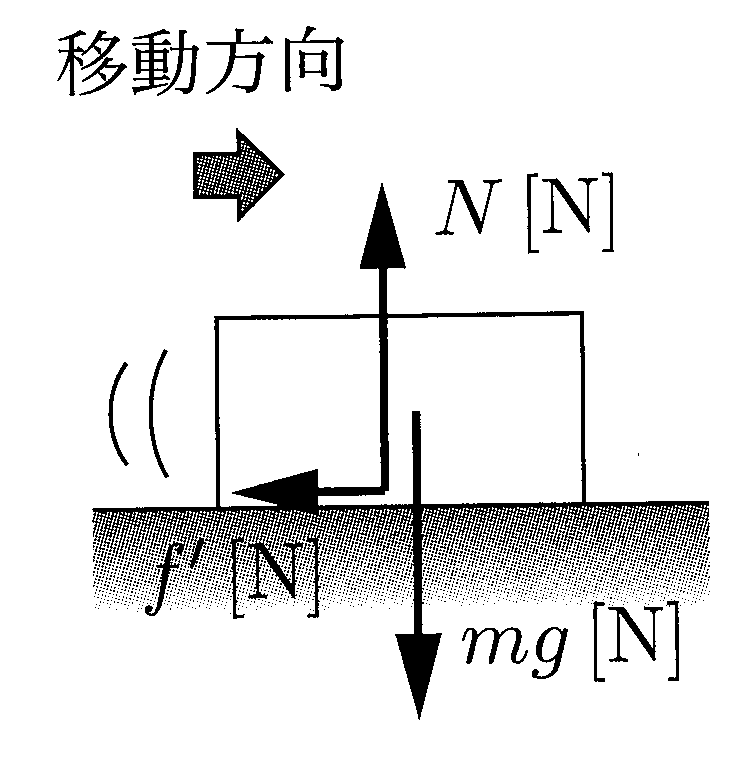
\includegraphics[keepaspectratio,width=40mm]
  {text_p22_fig1.png}
\end{wrapfigure}

互いに接触している2つの物体がこすれ合うように相対的に運動している場合，接触面がなめらかでないときは運動を妨げるような向きに摩擦力が作用する．
この摩擦力を{\bf 動摩擦力}という．

静止摩擦力と違い，{\bf 動摩擦力の大きさは（垂直抗力が一定ならば）常に一定}である．
接触面間の垂直抗力を$N$[N]とすると動摩擦力の大きさ$f'$[N]は
\[ f'=\mu'N\]
で与えられる．
比例定数$\mu'$を接触面の{\bf 動摩擦係数}という．

{\bf 動摩擦力は最大静止摩擦力よりも必ず小さい．}
そのため，静止摩擦係数$\mu_0$と動摩擦係数$\mu'$の間には
\[ \mu_0>\mu'\]
の関係が成立している．
$\mu_0と\mu'$は物体の速度$v$に依存しない．

\begin{matome}{動摩擦力}
 \hspace{5mm} 摩擦のある2物体同士の相対運動$\Rightarrow $動摩擦力が作用\\
 \hspace{5mm} 大きさは常に$\mu'N$，相対運動を妨げる向きに作用
 \end{matome}


 \ 
 
%\begin{breakbox}
%\ex＜力の作図と運動方程式の立式＞\\
%\begin{wrapfigure}[4]{r}[5mm]{70mm}
%  \centering
%  \vspace{-5mm}
%  \includegraphics[keepaspectratio,width=60mm]
%  {text_p22_fig2.png}
%\end{wrapfigure}
%\hspace{5mm}粗い水平面上で質量$m$[kg]の物体に初速度$v_0$[m/s]を与えて滑らせたときの運動について以下の問いに答えよ．ただし，床と物体の間の動摩擦係数を$\mu'$，重力加速度の大きさを$g [{\rm m/s^2}]$とする．
%\begin{description}
%\item[(1)] 物体の持つ右向きの加速度$a [{\rm m/s^2}]$を求めよ．
%\item[(2)] 物体が静止するのに要する時間$t_1$[s]およびそれまでに滑った距離$\Delta x$[m]を求めよ．
%\end{description}
%
%\end{breakbox}


%\subsection{運動方程式の立式}
%
%ここまで学んできた知識を用いて，実際に運動方程式を立てる練習を行う．
%
% \ 
% 
%\begin{breakbox}
%\ex＜力の作図と運動方程式の立式＞\\
%\begin{wrapfigure}[8]{r}[5mm]{70mm}
%  \centering
%  \vspace{-5mm}
%  \includegraphics[keepaspectratio,width=60mm]
%  {text_p23_fig1.png}
%\end{wrapfigure}
%\hspace{5mm}水平面上に固定された粗い斜面を持つ傾斜角$\theta$の斜面台に滑車を取り付け，質量$M$[kg]の物体Aと質量$m$[kg]の物体Bを糸を用いて図のようにつなげてつるす．
%Bを手で押さえておき，糸をぴんと張った状態にしておいた上でそっと手を離すときについて以下の問いに答えよ．
%ただし，糸や定滑車の質量は無視でき，Bと斜面との間の静止摩擦係数を$\mu_0$，動摩擦係数を$\mu'$とし，重力加速度の大きさを$g [{\rm m/s^2}]$とする．
%\begin{description}
%\item[(1)] Bをそっと手放したとき，Bはそのまま静止していたという．このときの$M,m$の間の関係式を与えられた適当な文字を用いて不等式で表せ．
%\item[(2)] Bをそっと手放したとき，Bが上昇していくために必要な条件式を表せ．
%\item[(3)] Bをそっと手放したとき，Bは斜面を滑り降りたという．これに必要な条件式および，このときBが斜面を滑り降りる加速度を求めよ．
%\end{description}
%
%\end{breakbox}



\newpage

\begin{figure}[h]
\begin{center}
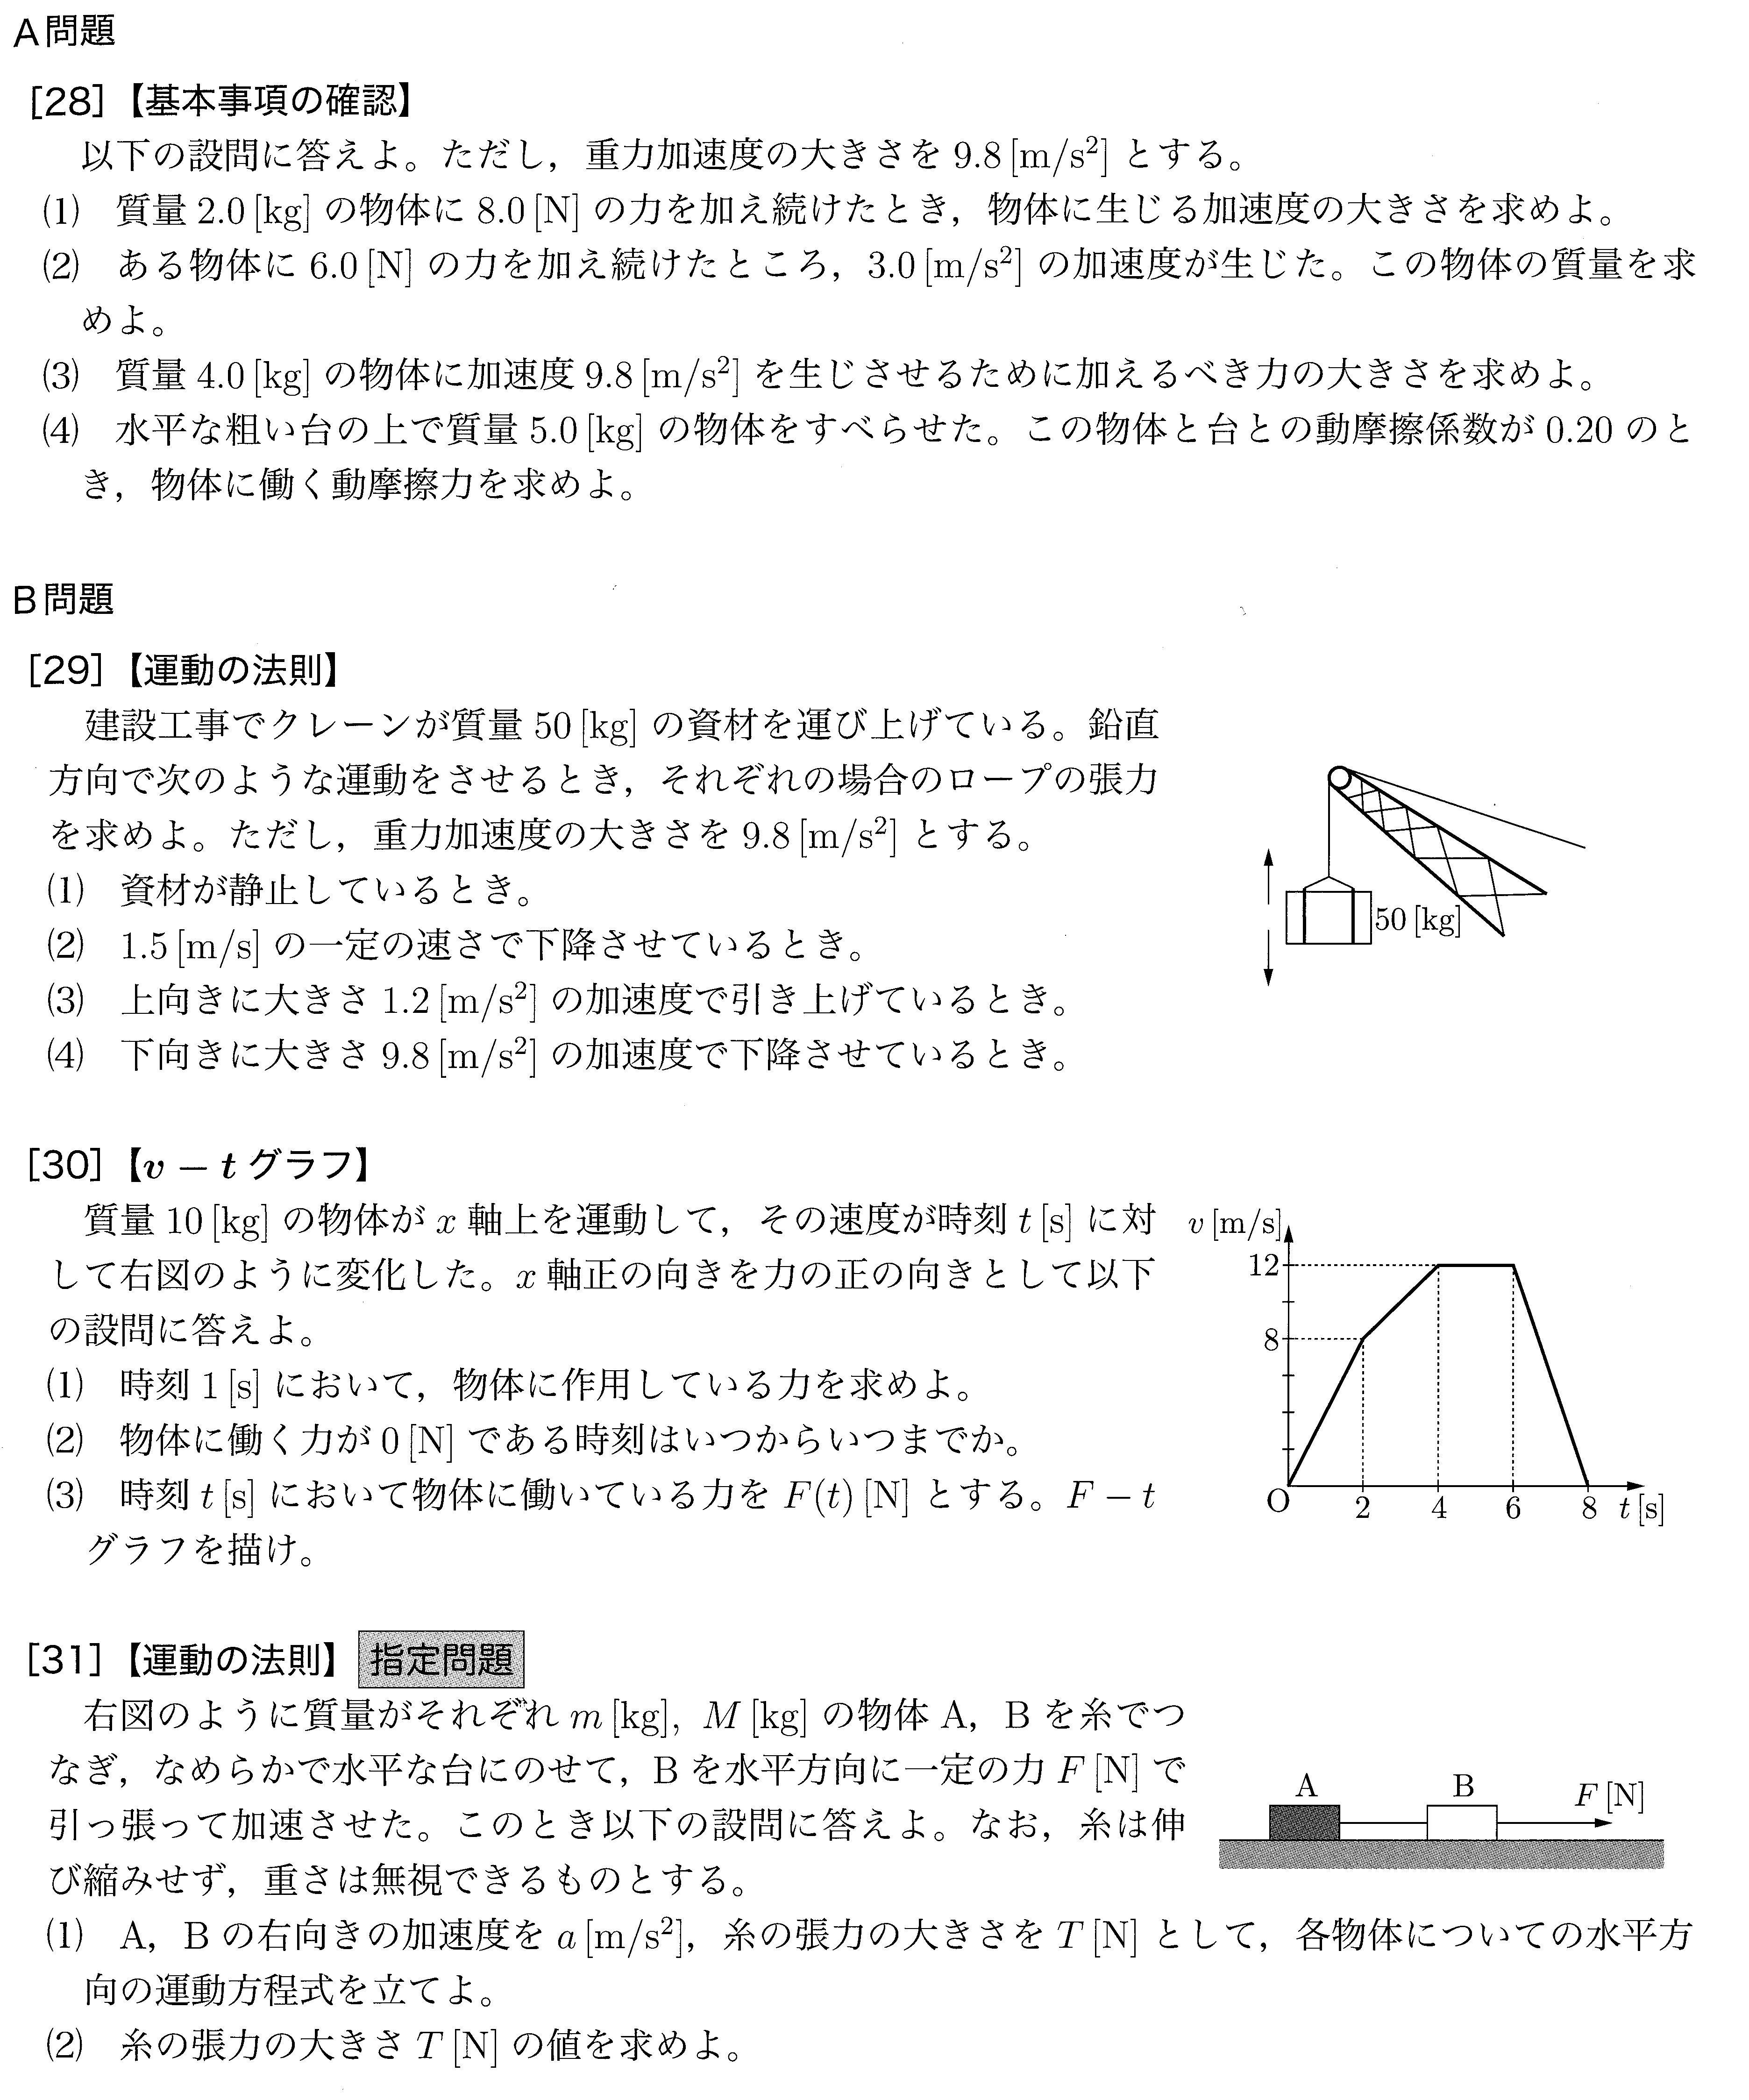
\includegraphics[width=170mm]{prob_p11.png}
\end{center}
\end{figure}

\newpage

\begin{figure}[h]
\begin{center}
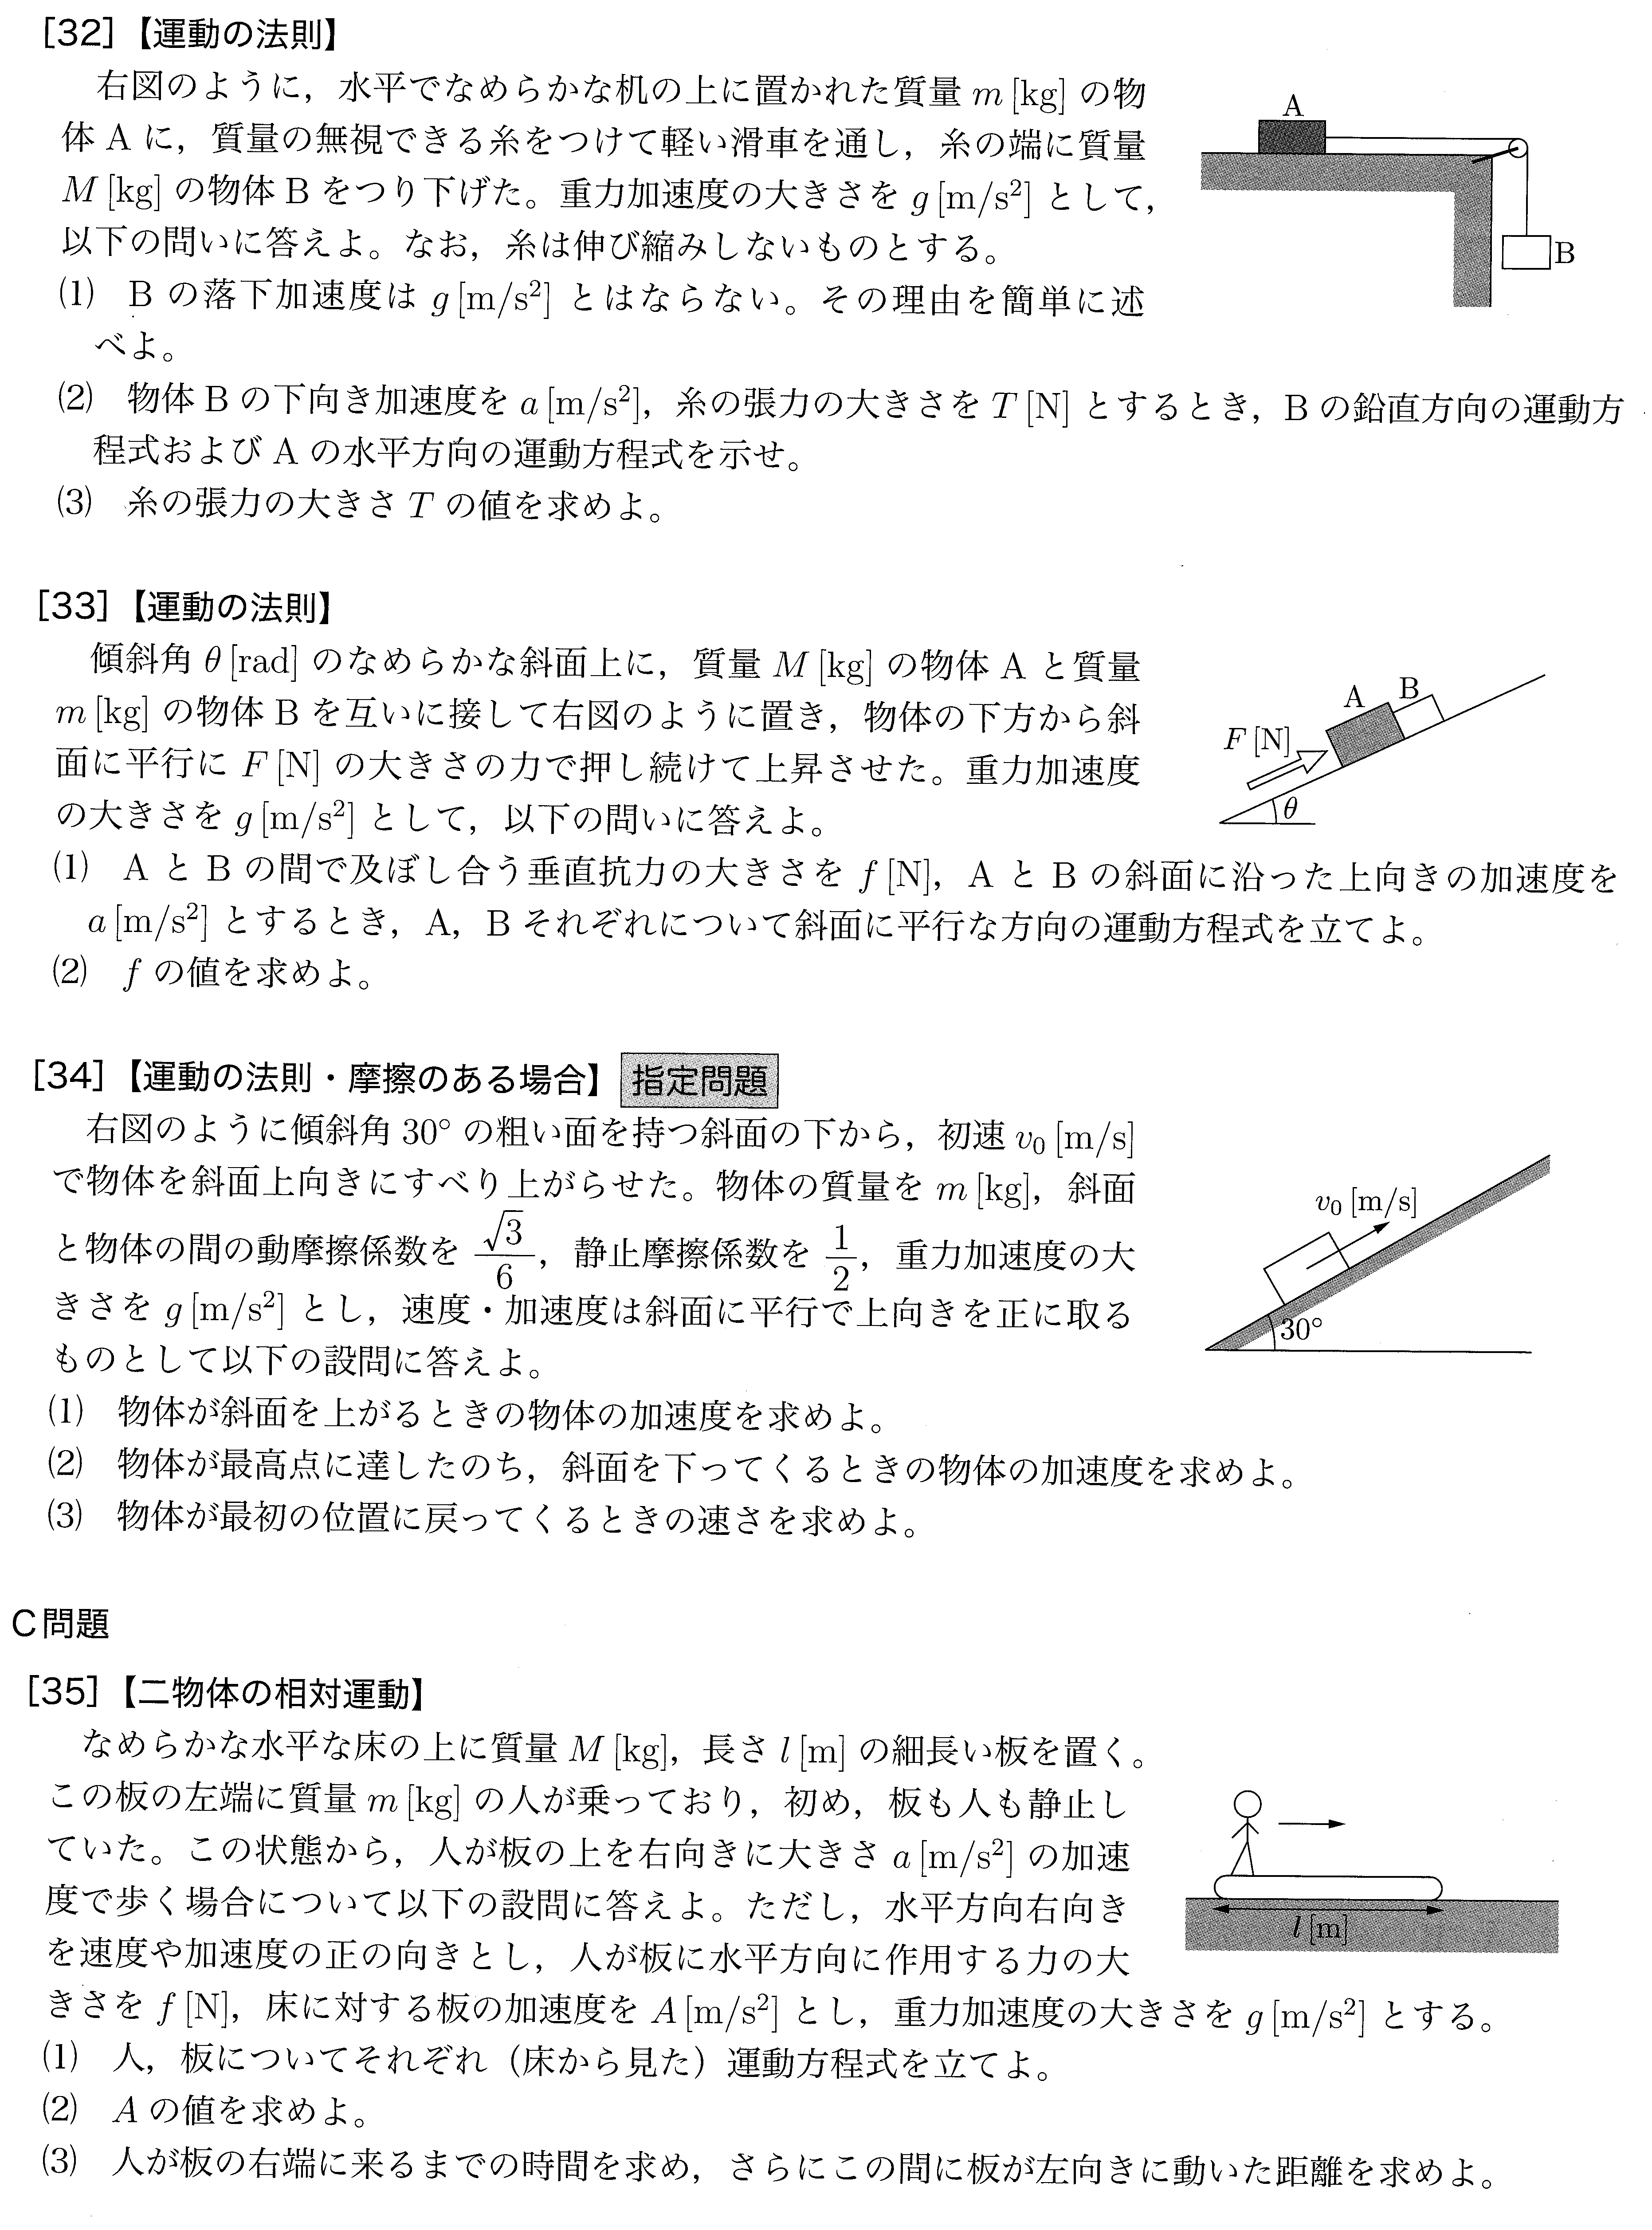
\includegraphics[width=170mm]{prob_p12.png}
\end{center}
\end{figure}

\newpage

\begin{figure}[h]
\begin{center}
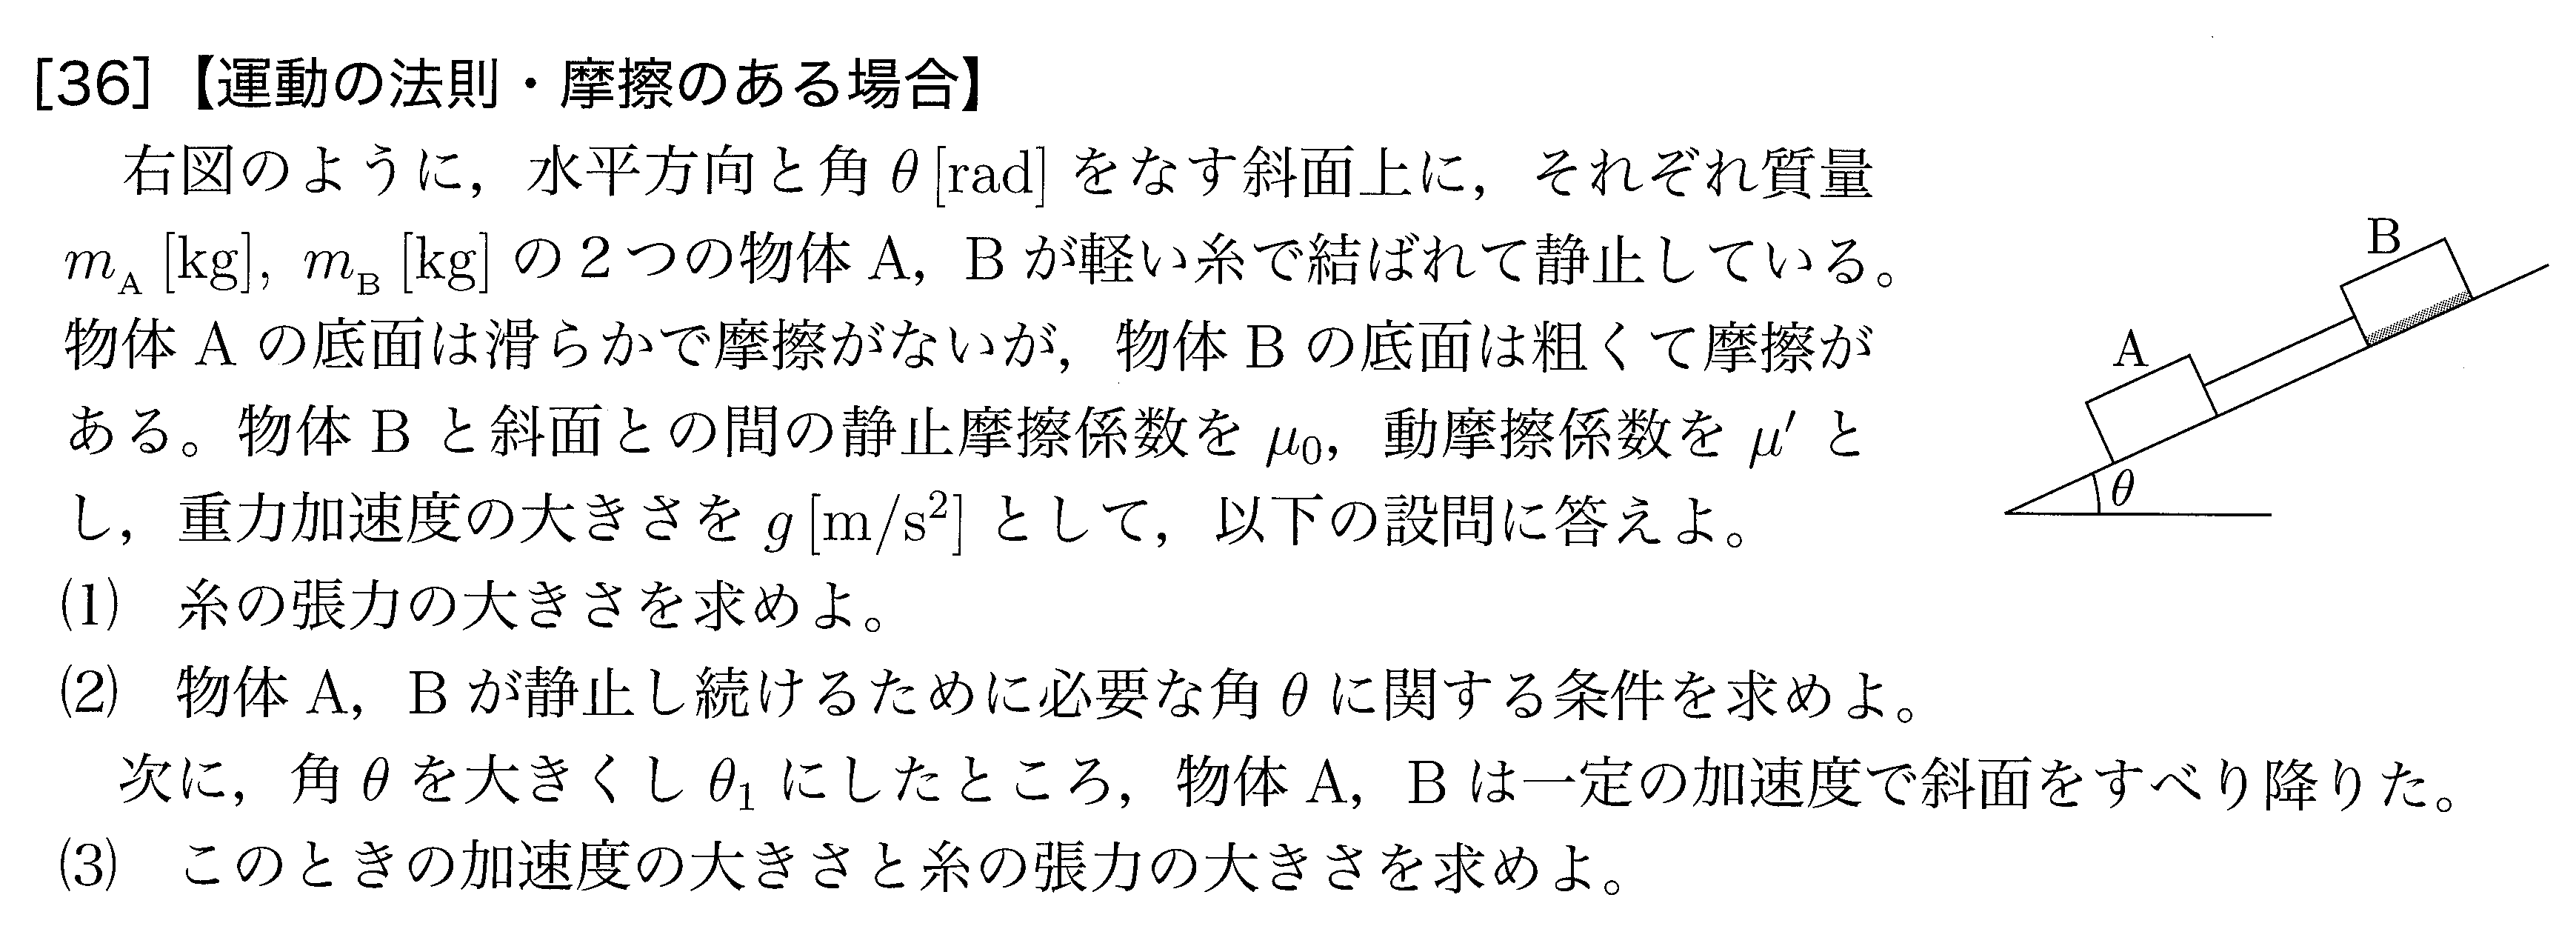
\includegraphics[width=170mm]{prob_p13.png}
\vspace{20cm}
\end{center}
\end{figure}

\newpage

\begin{figure}[h]
\begin{center}
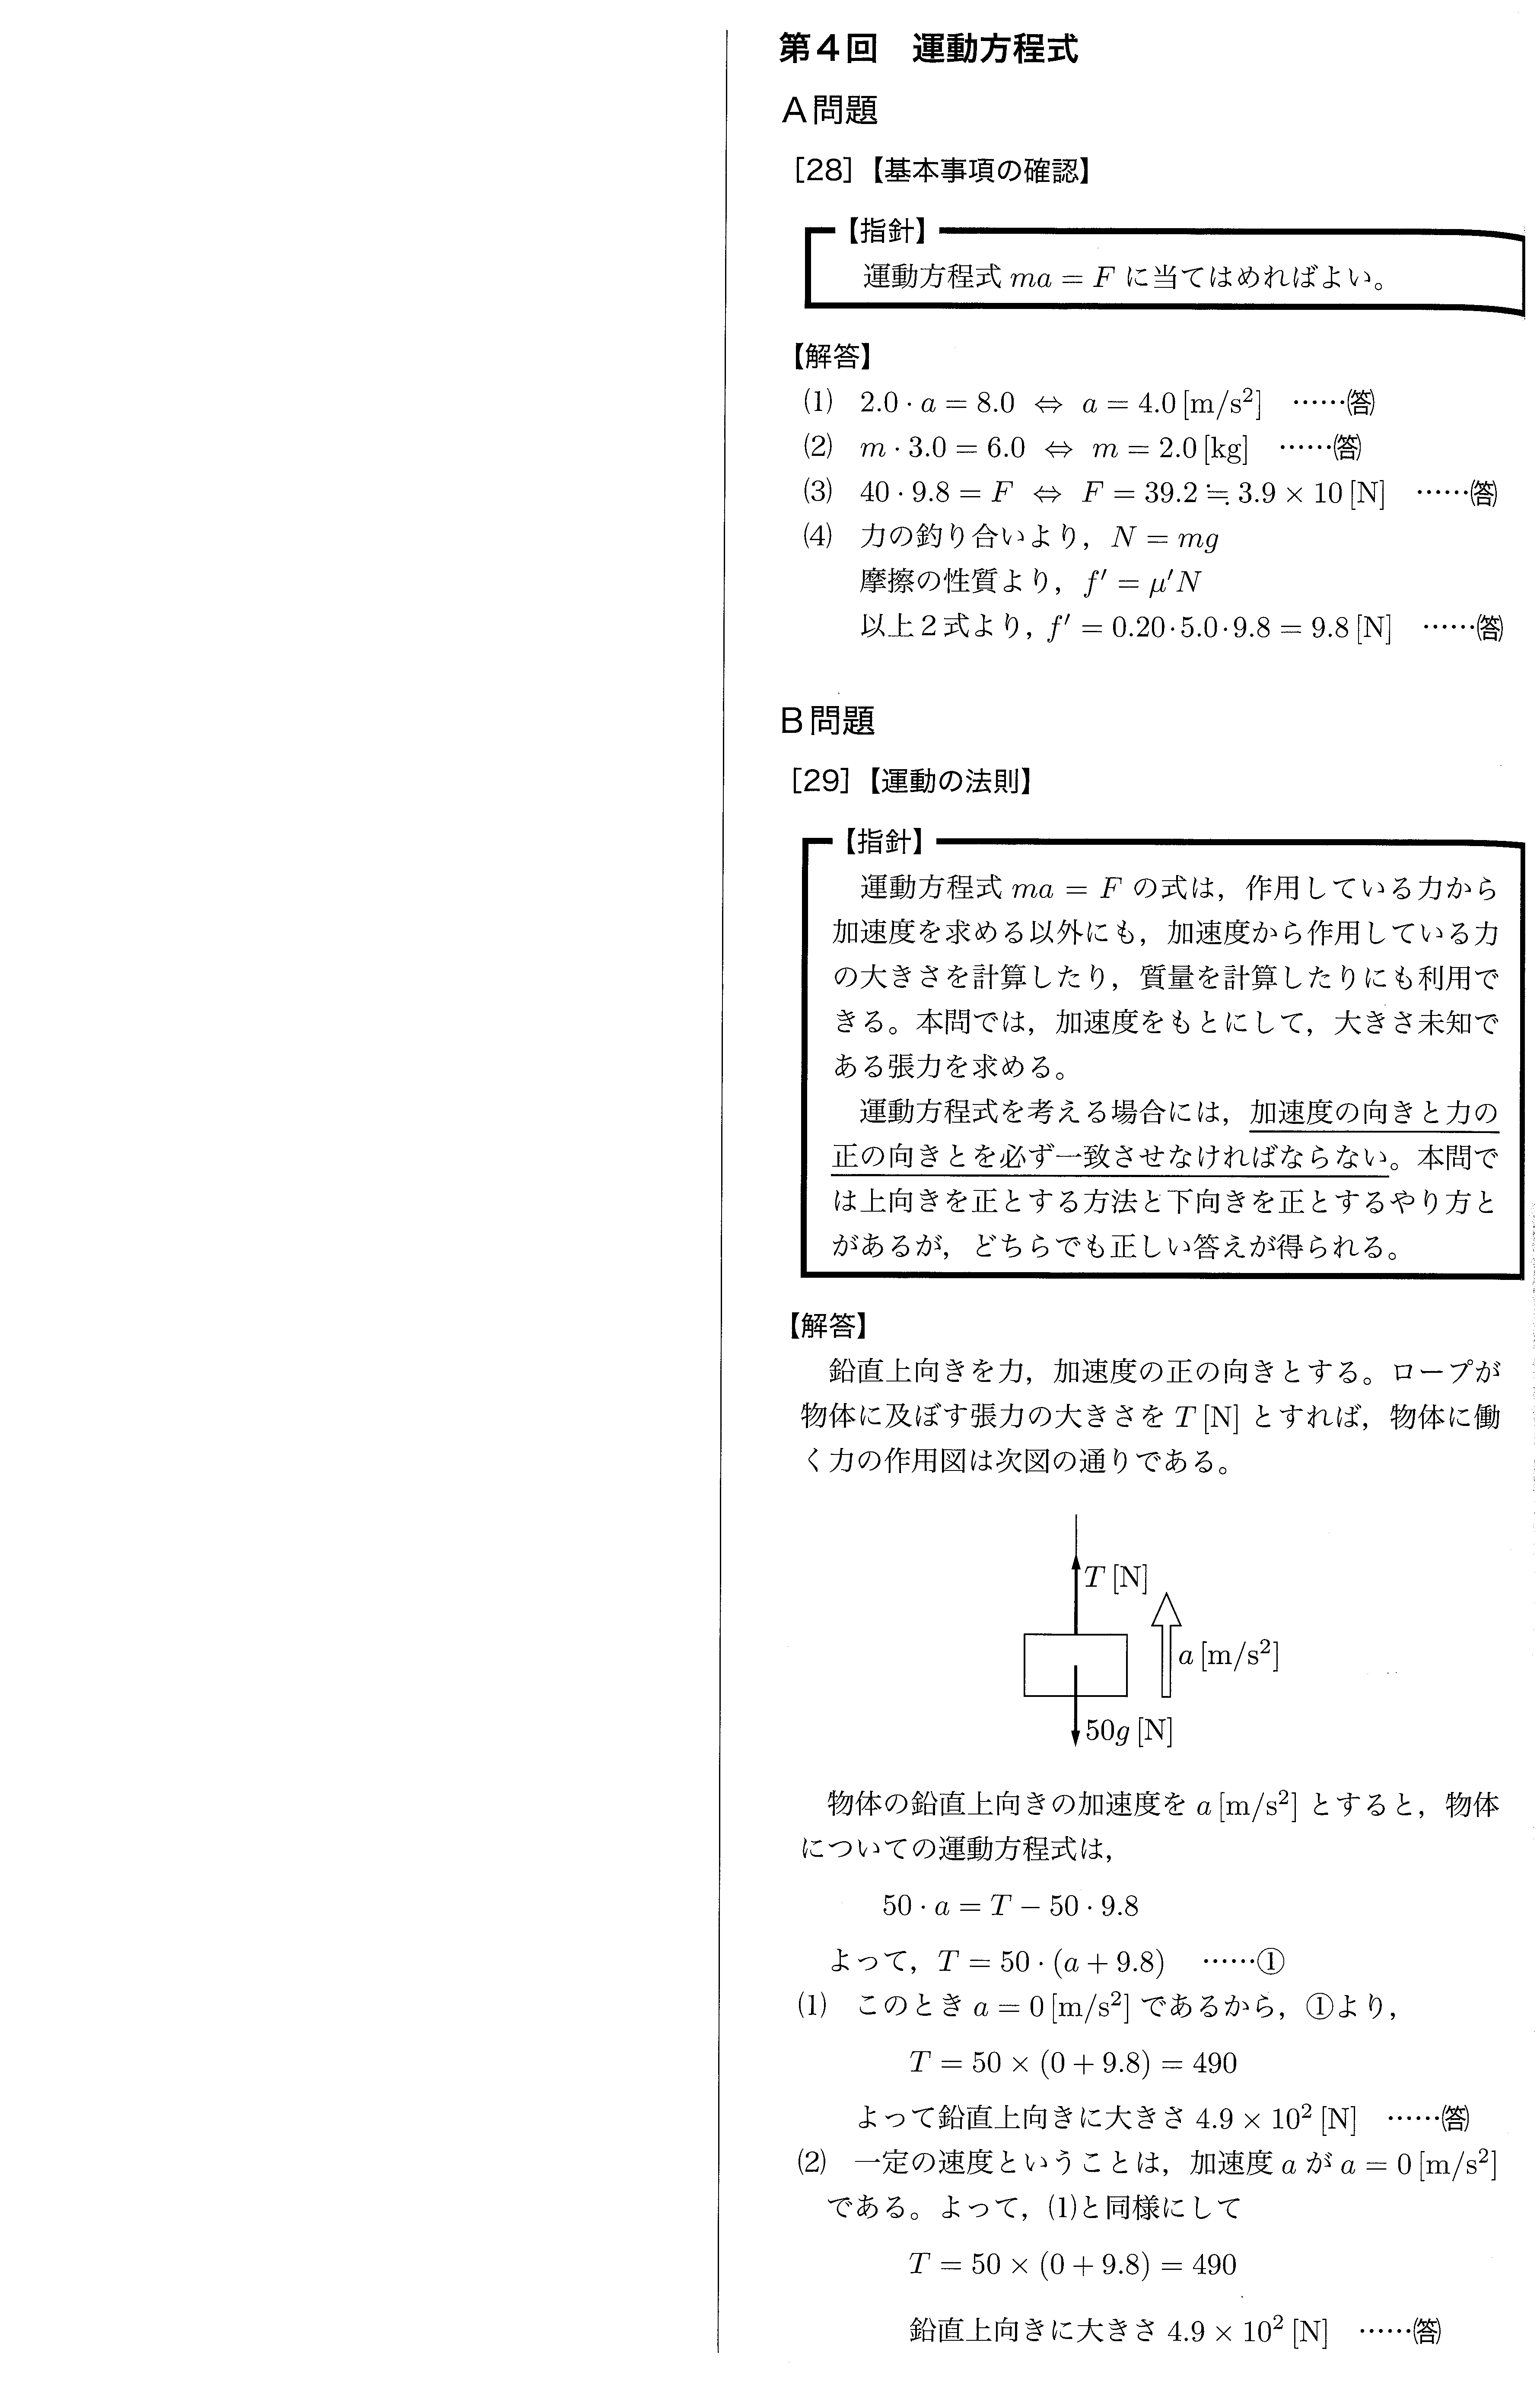
\includegraphics[width=170mm]{prob_p76_2.png}
\end{center}
\end{figure}

\newpage

\begin{figure}[h]
\begin{center}
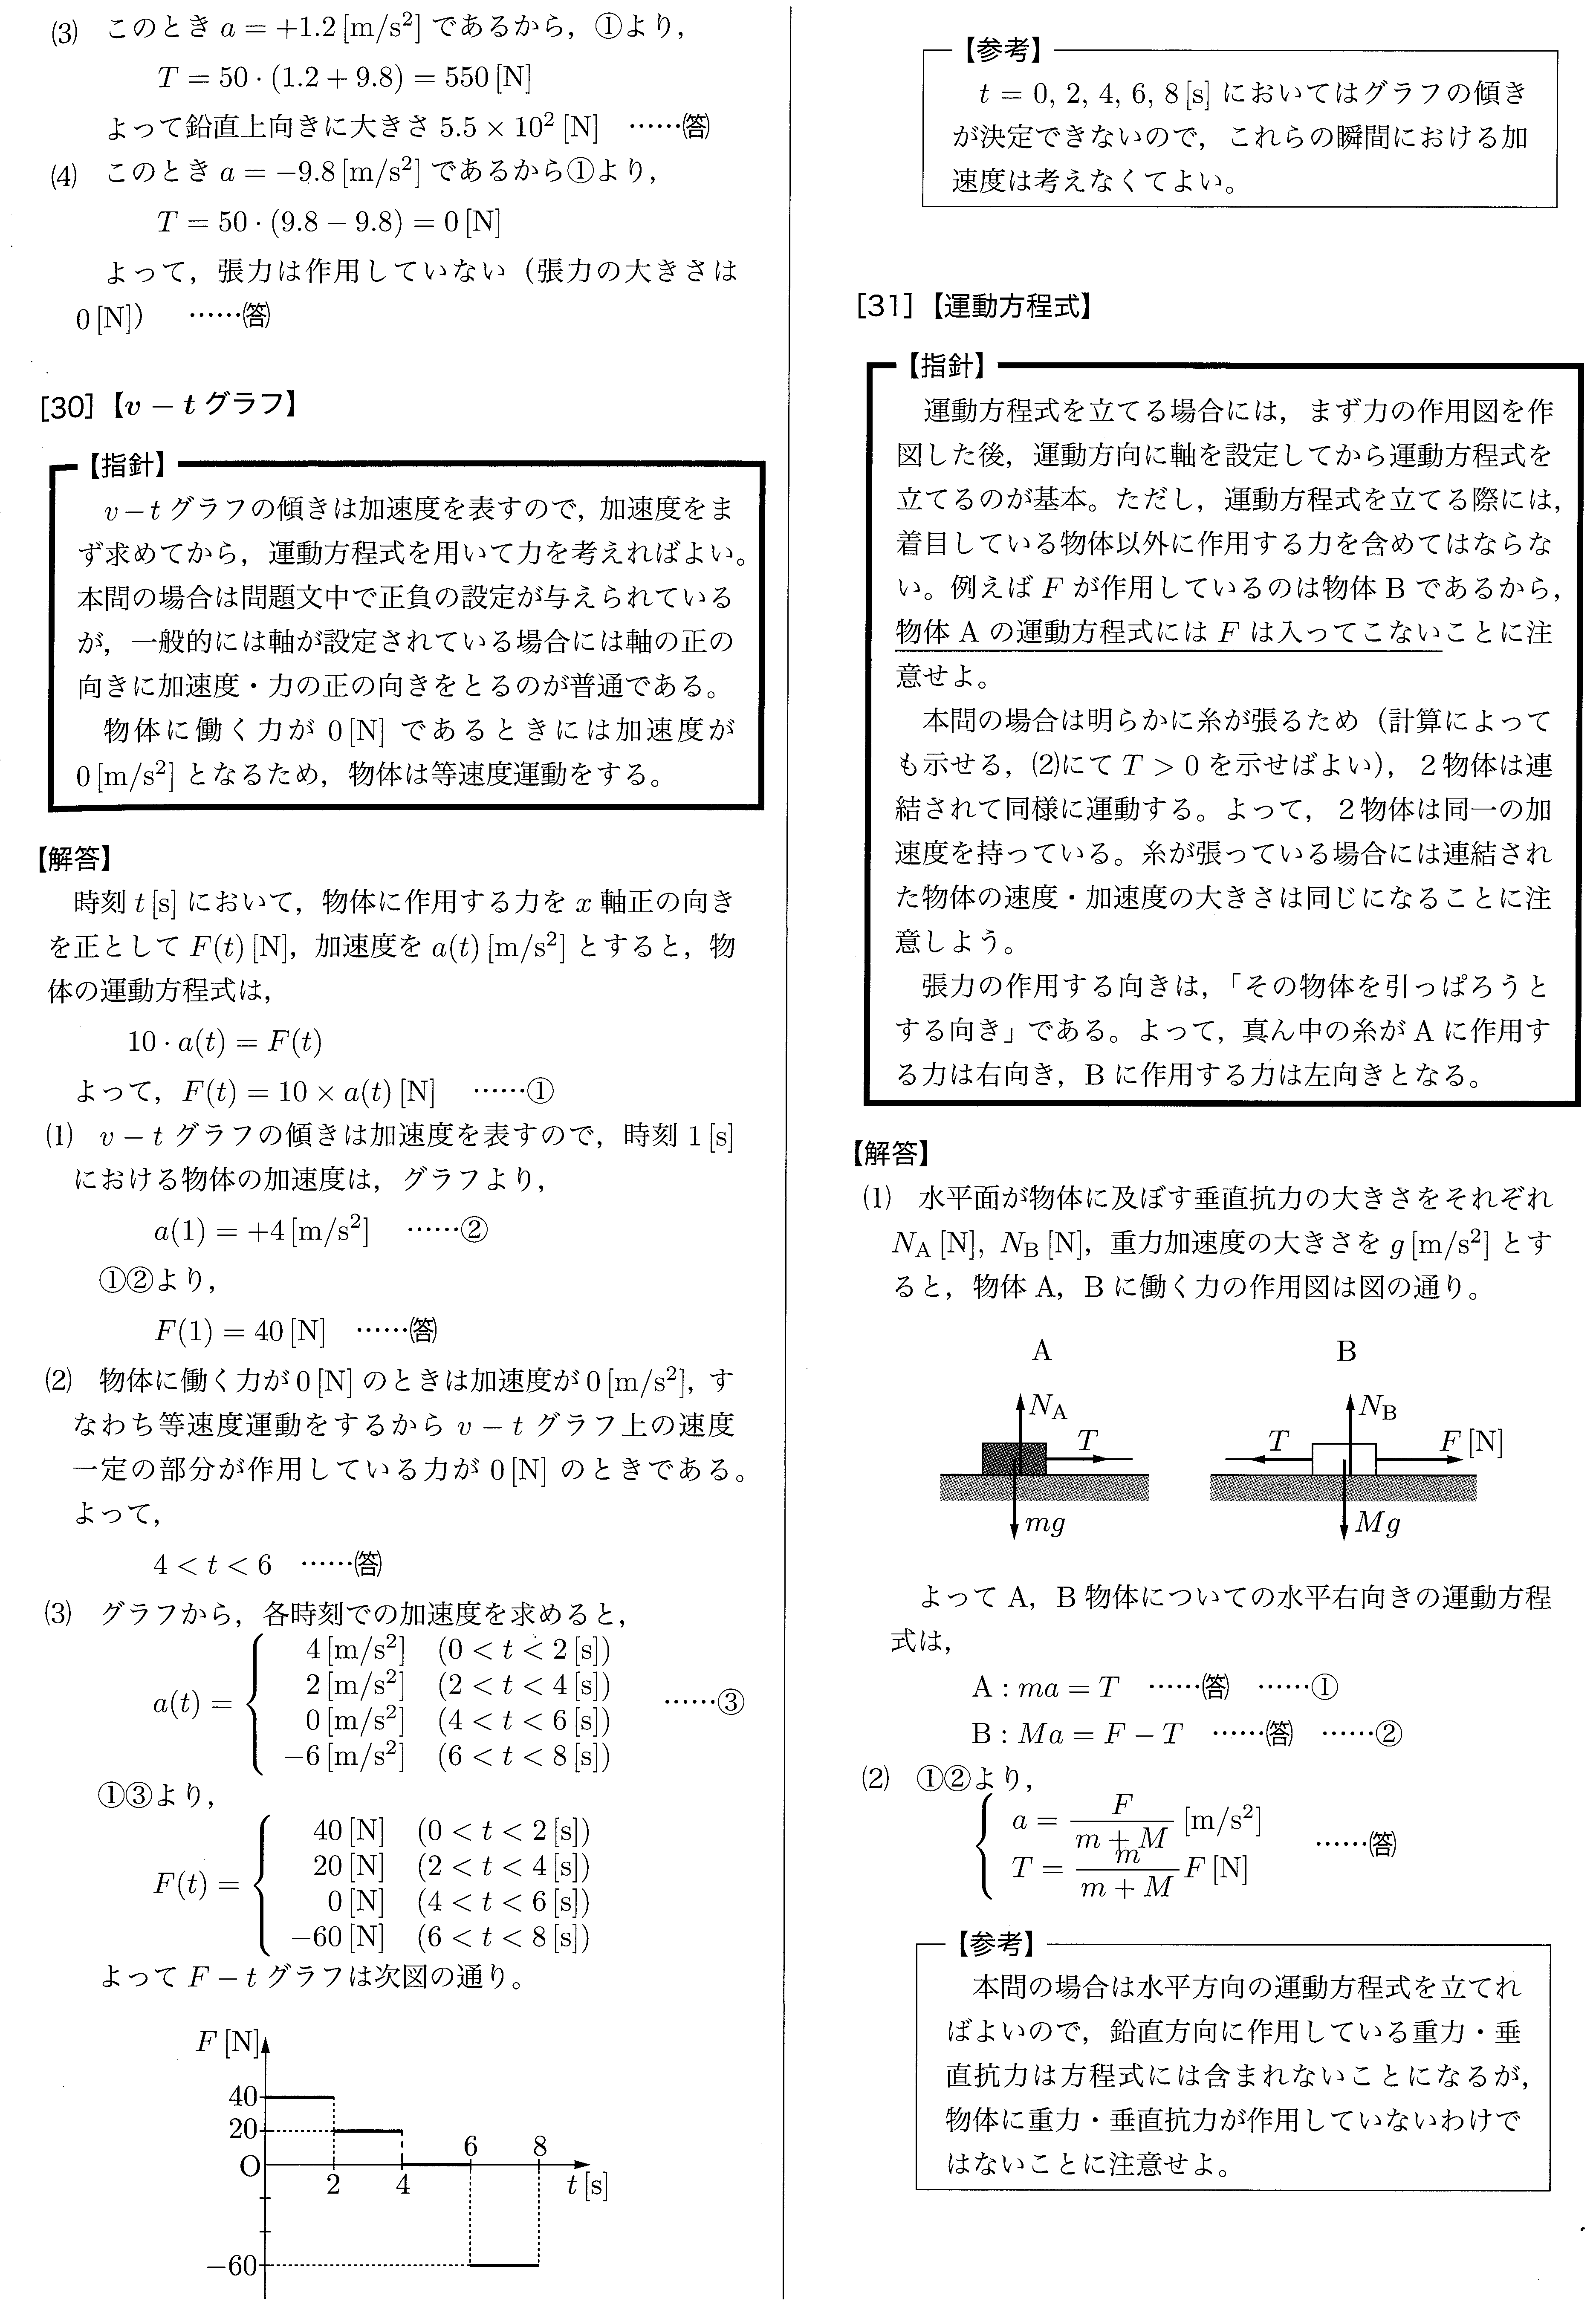
\includegraphics[width=170mm]{prob_p77.png}
\end{center}
\end{figure}

\newpage

\begin{figure}[h]
\begin{center}
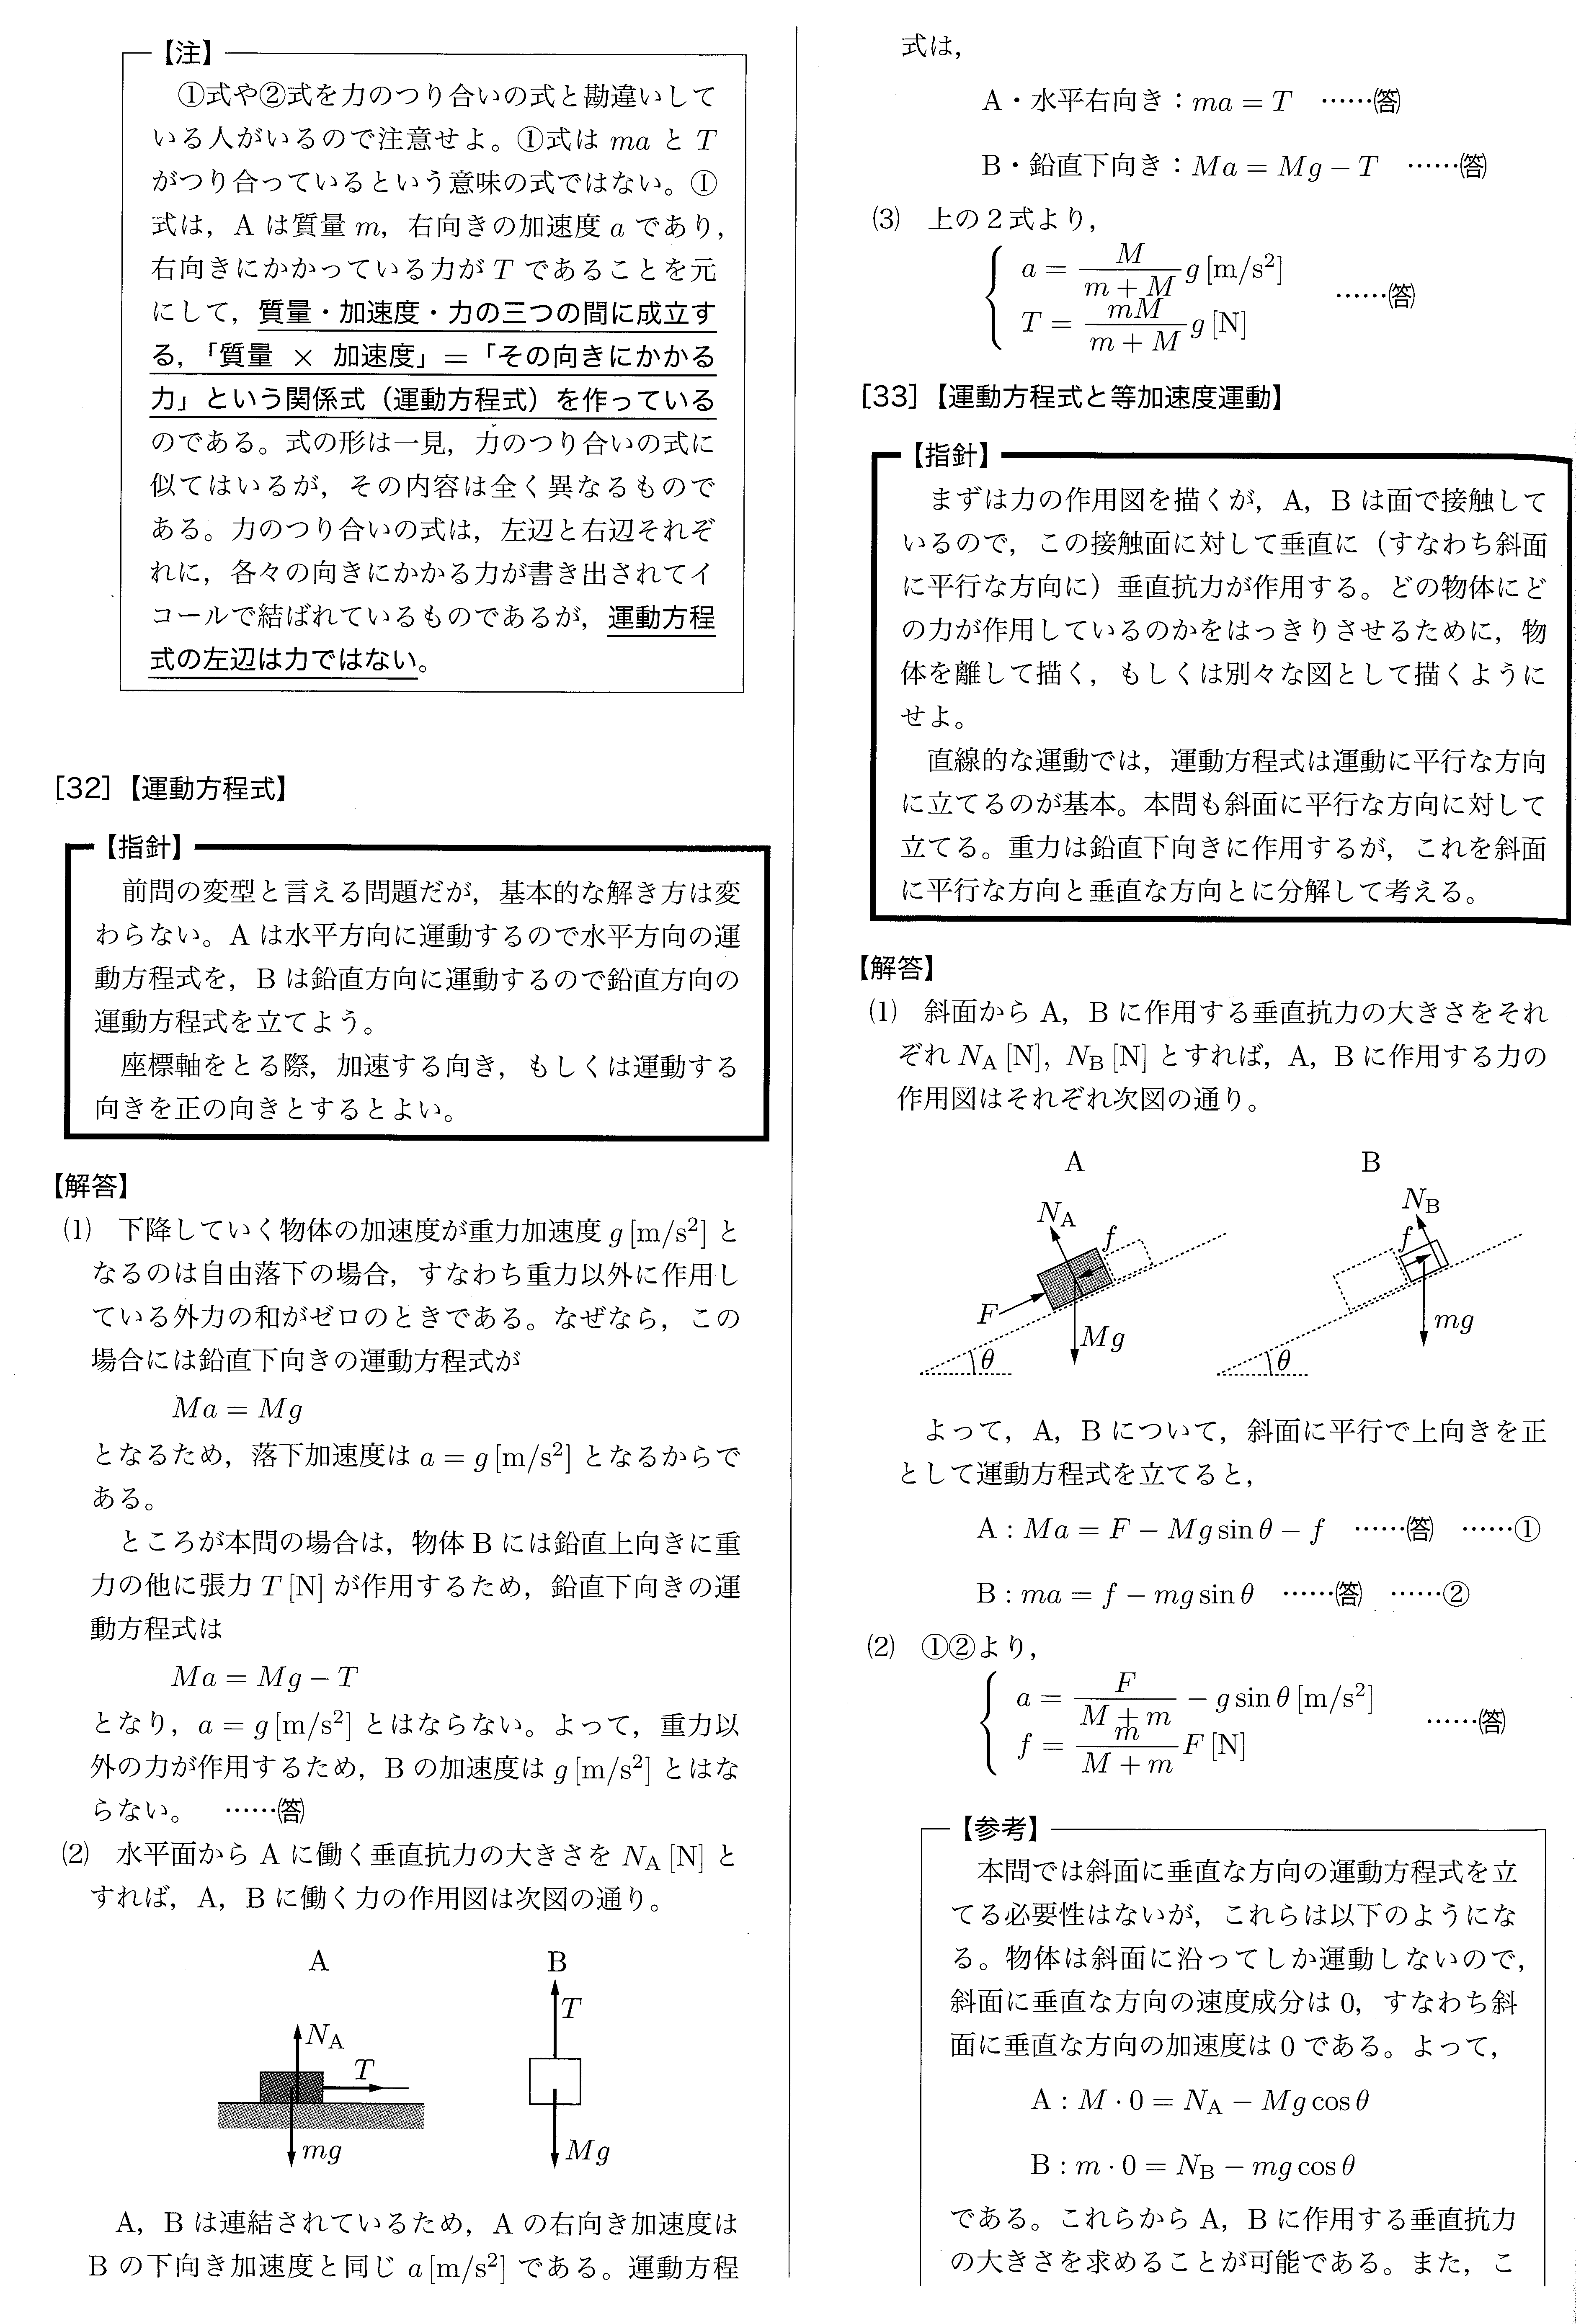
\includegraphics[width=170mm]{prob_p78.png}
\end{center}
\end{figure}

\newpage

\begin{figure}[h]
\begin{center}
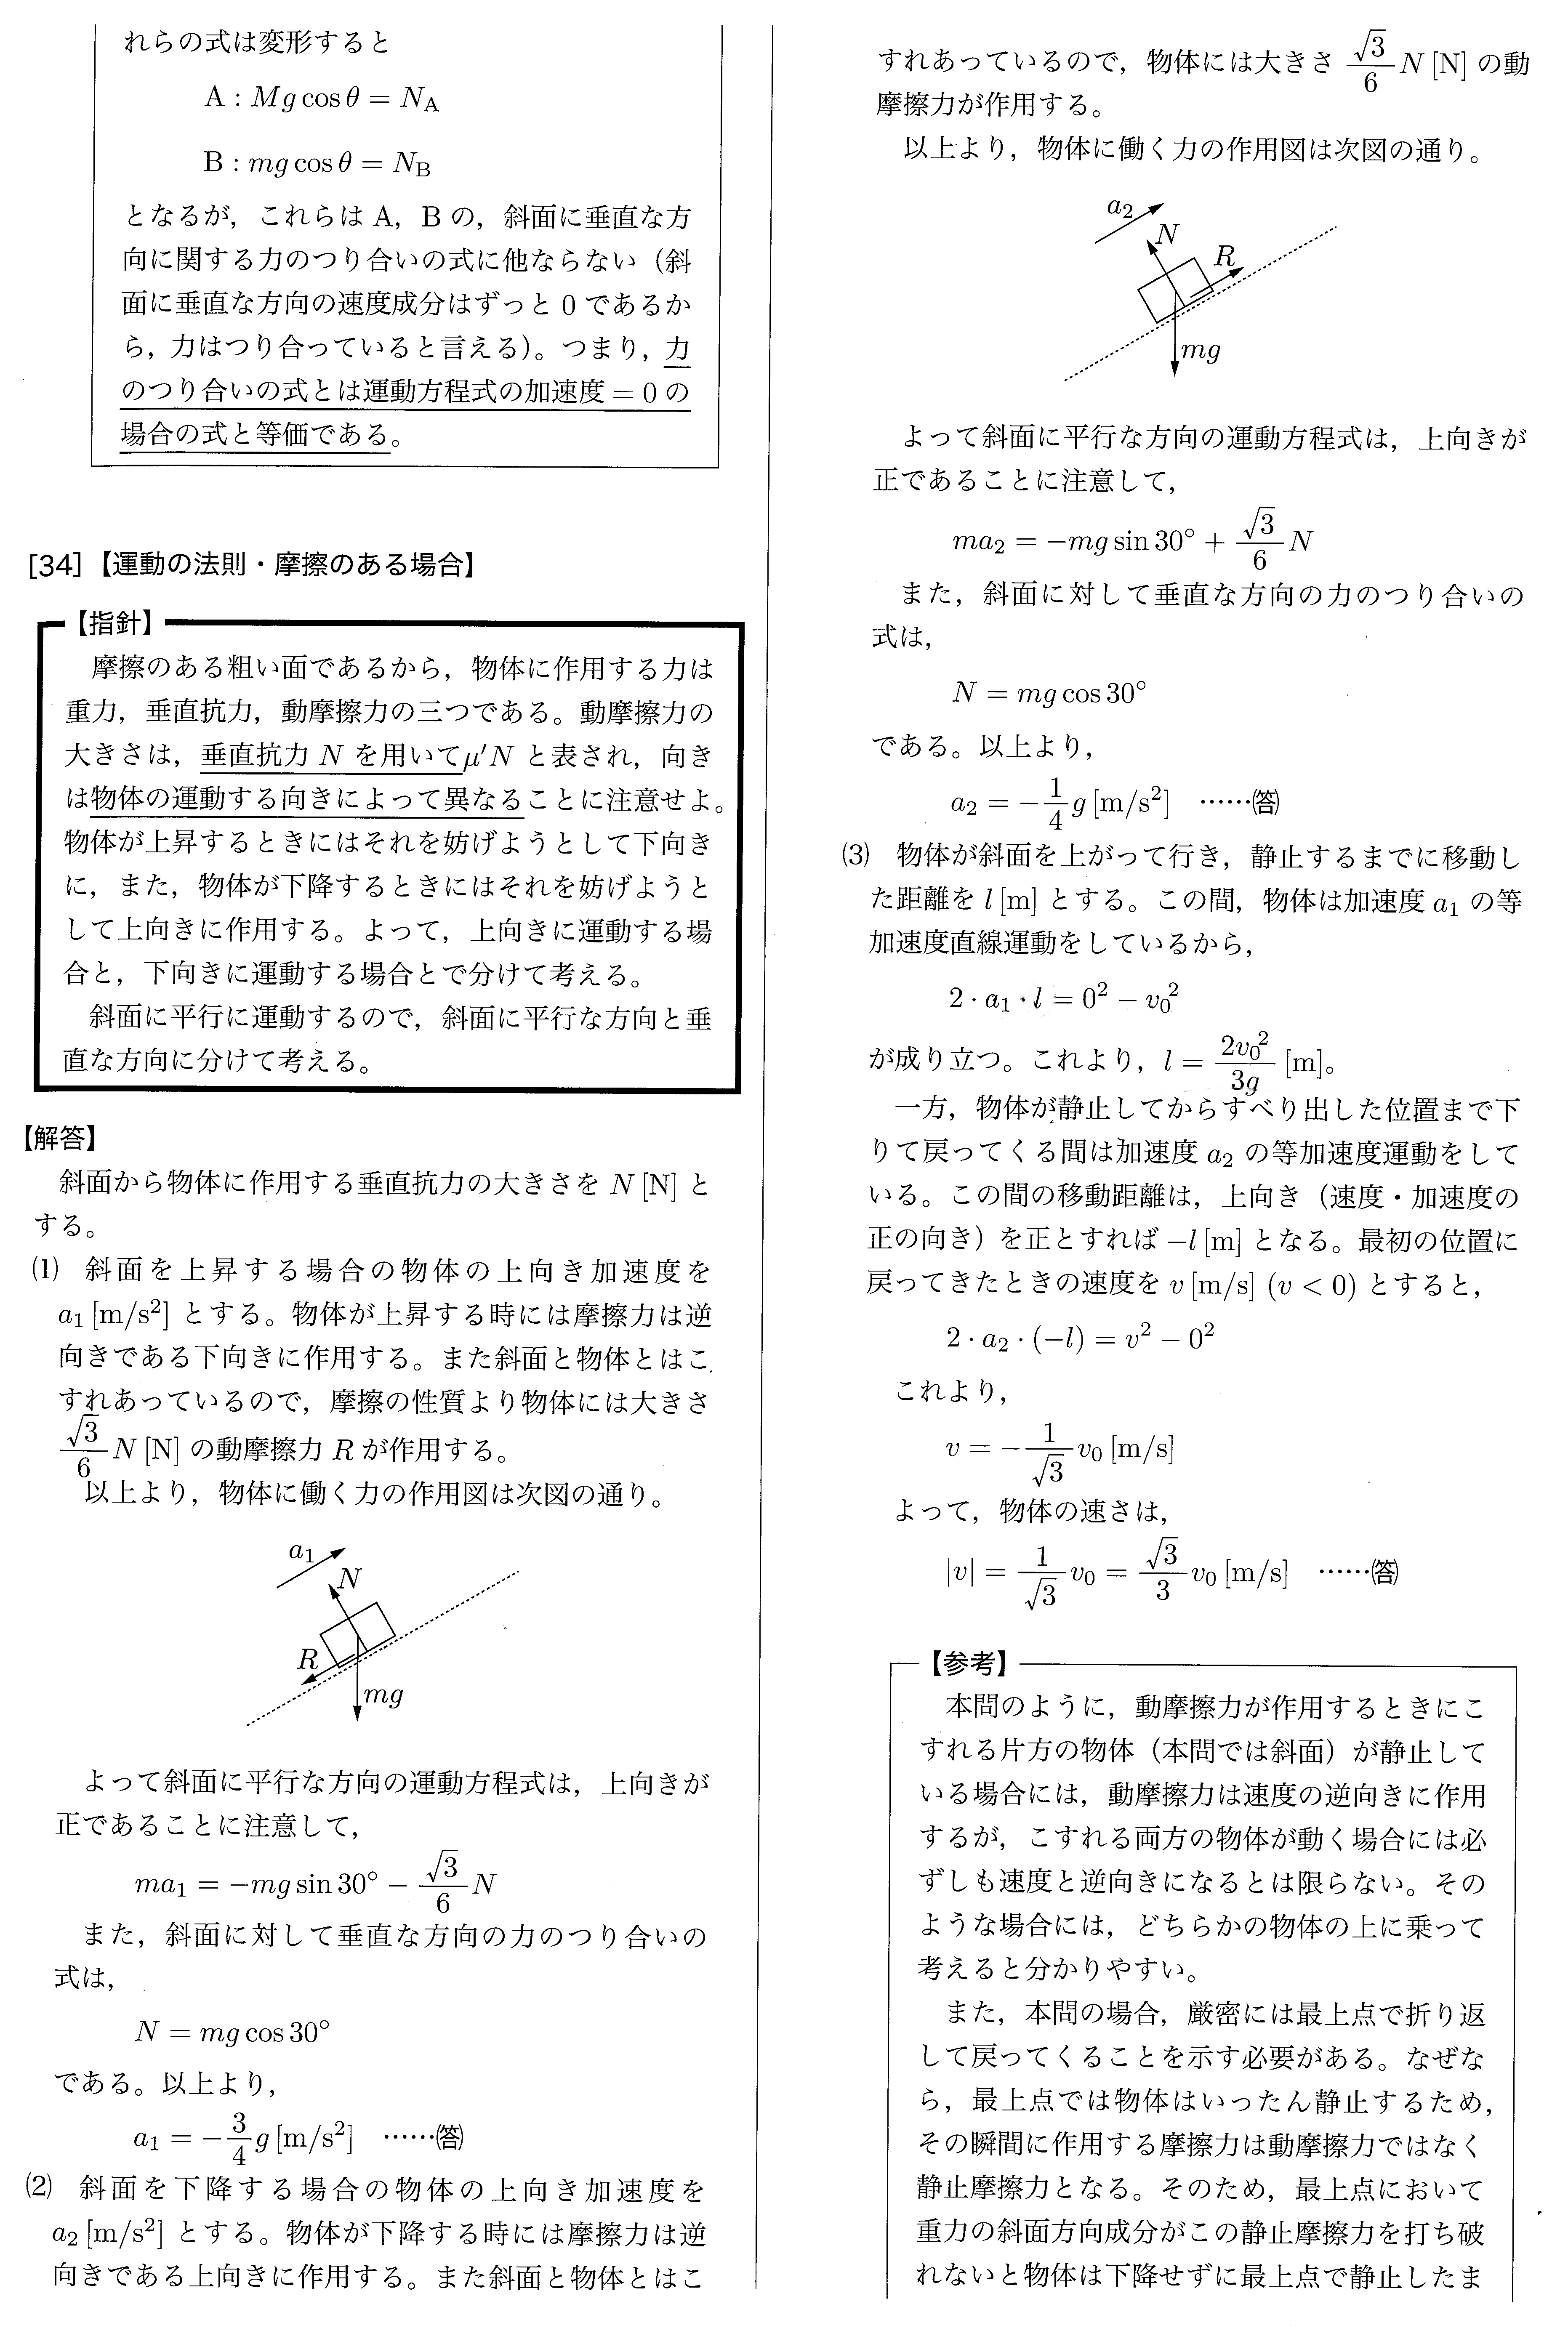
\includegraphics[width=170mm]{prob_p79.png}
\end{center}
\end{figure}

\newpage

\begin{figure}[h]
\begin{center}
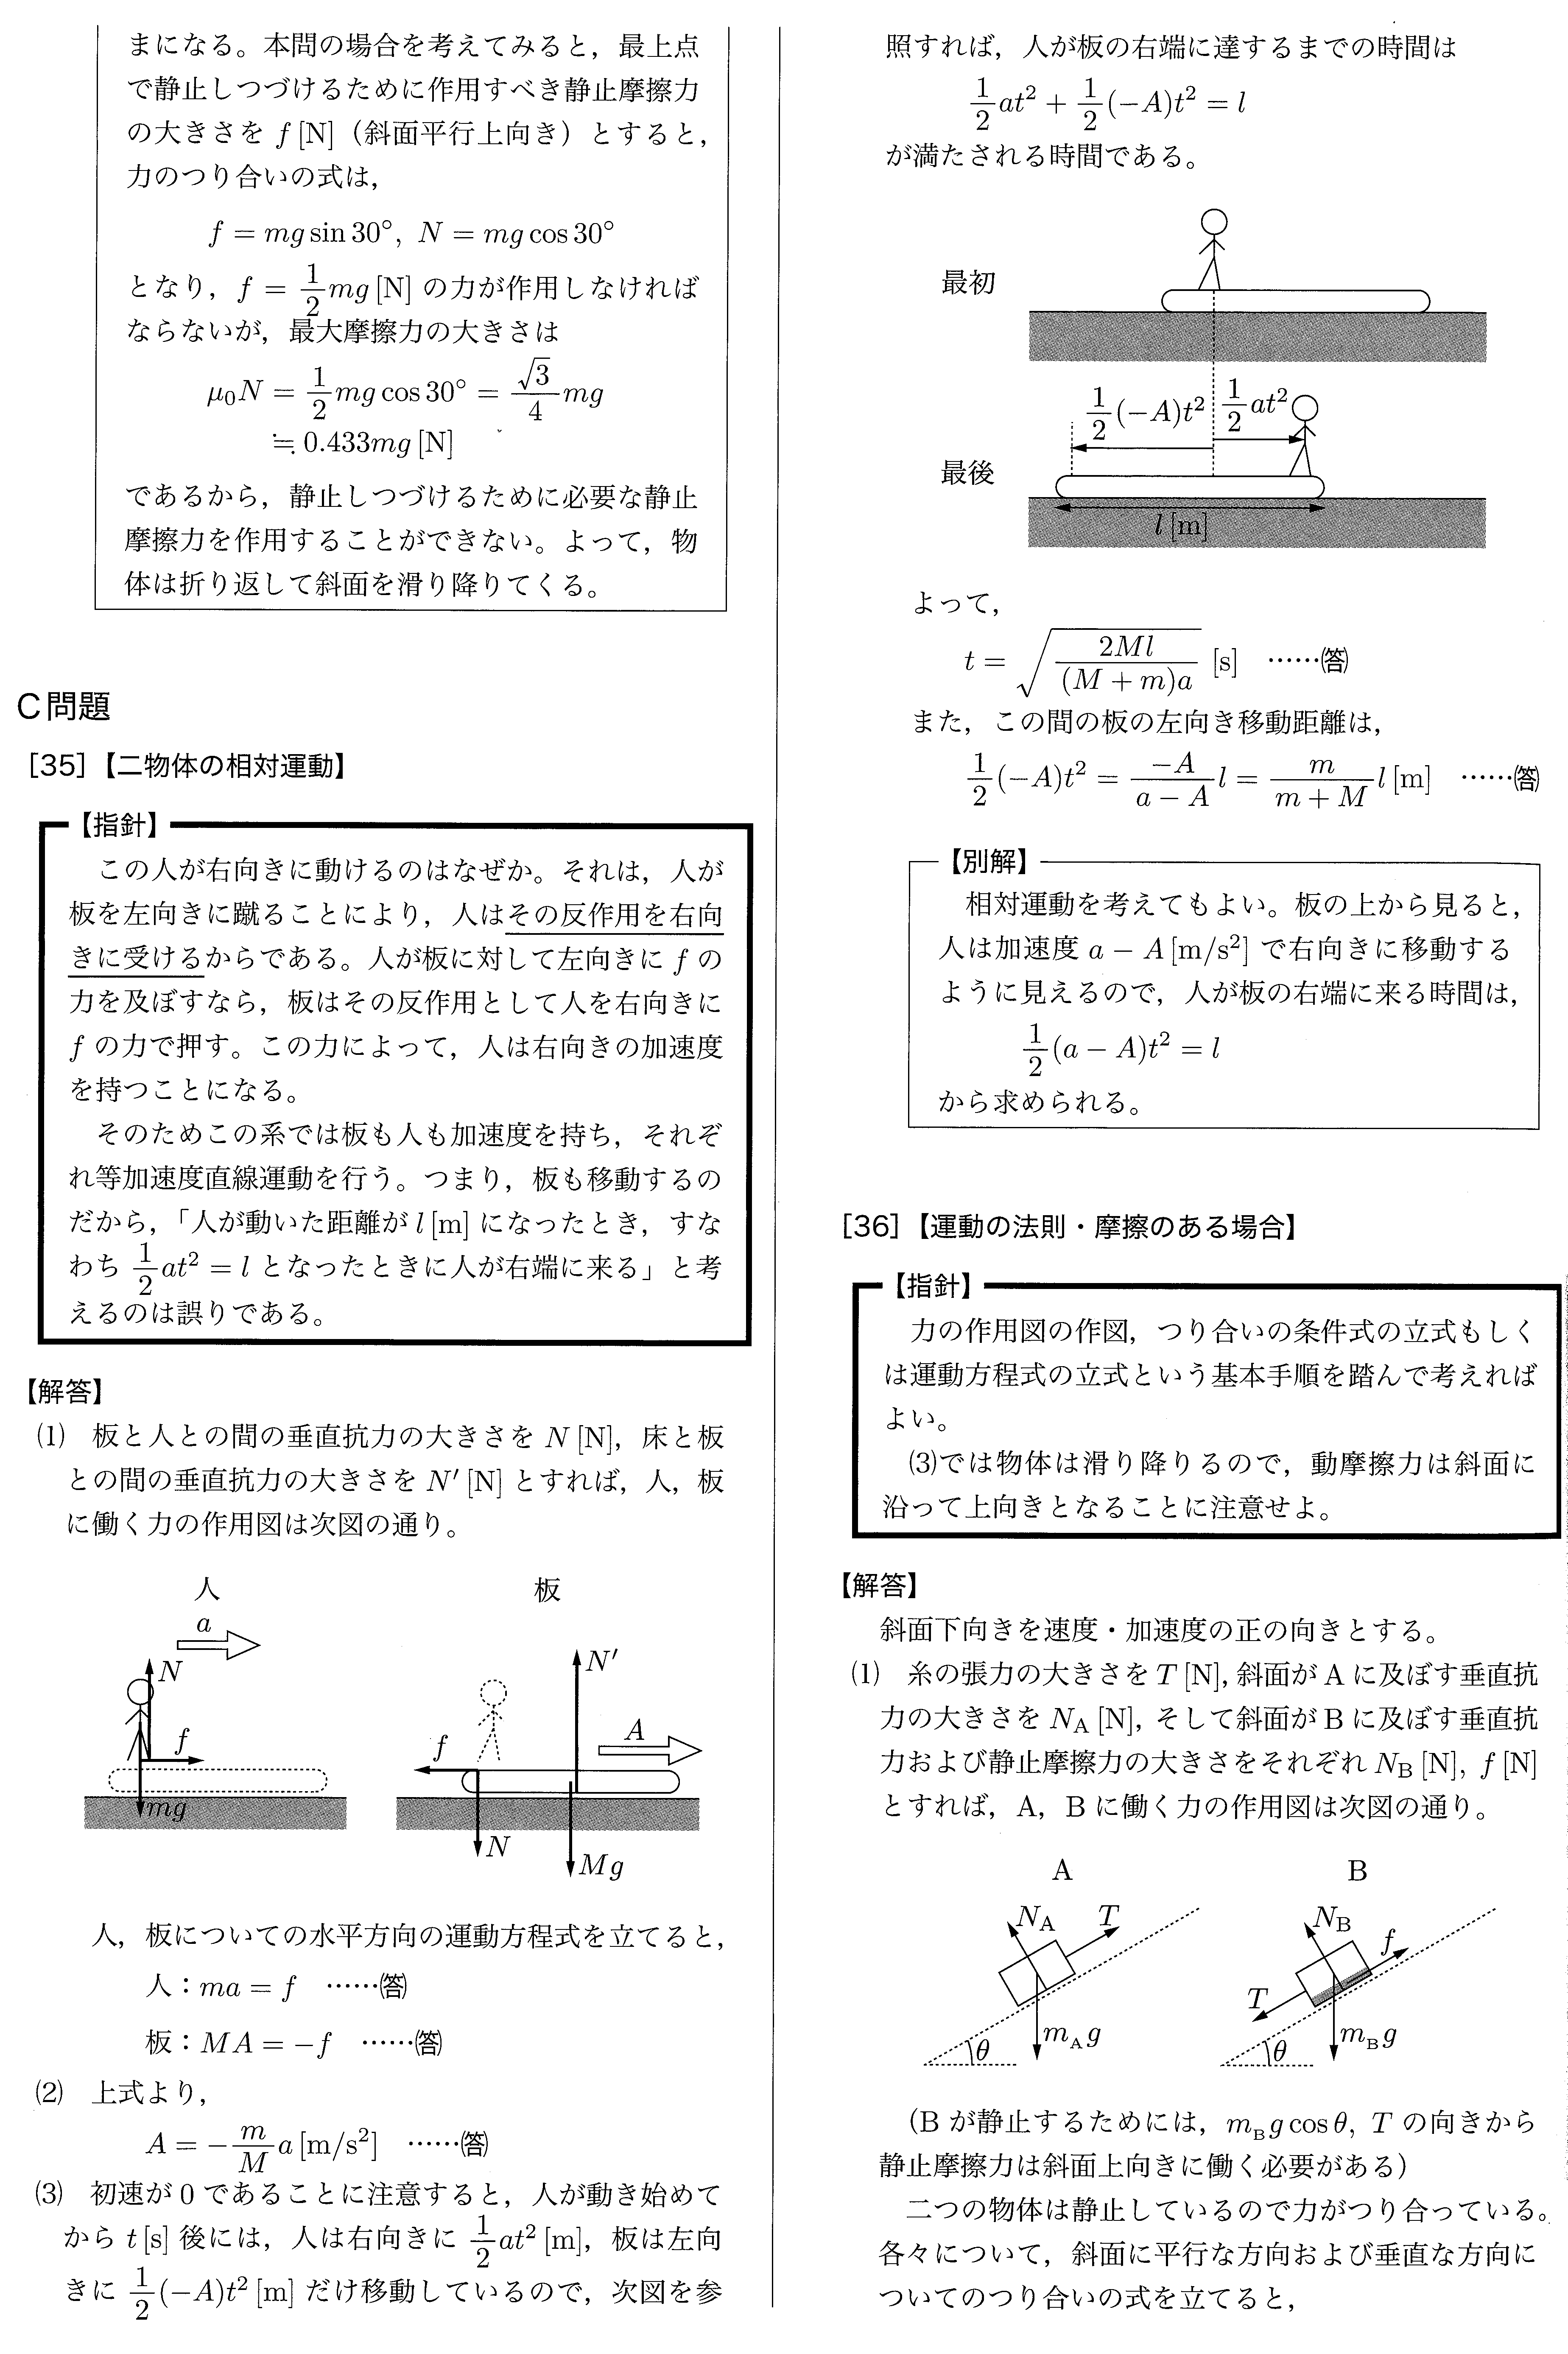
\includegraphics[width=170mm]{prob_p80.png}
\end{center}
\end{figure}

\newpage

\begin{figure}[h]
\begin{center}
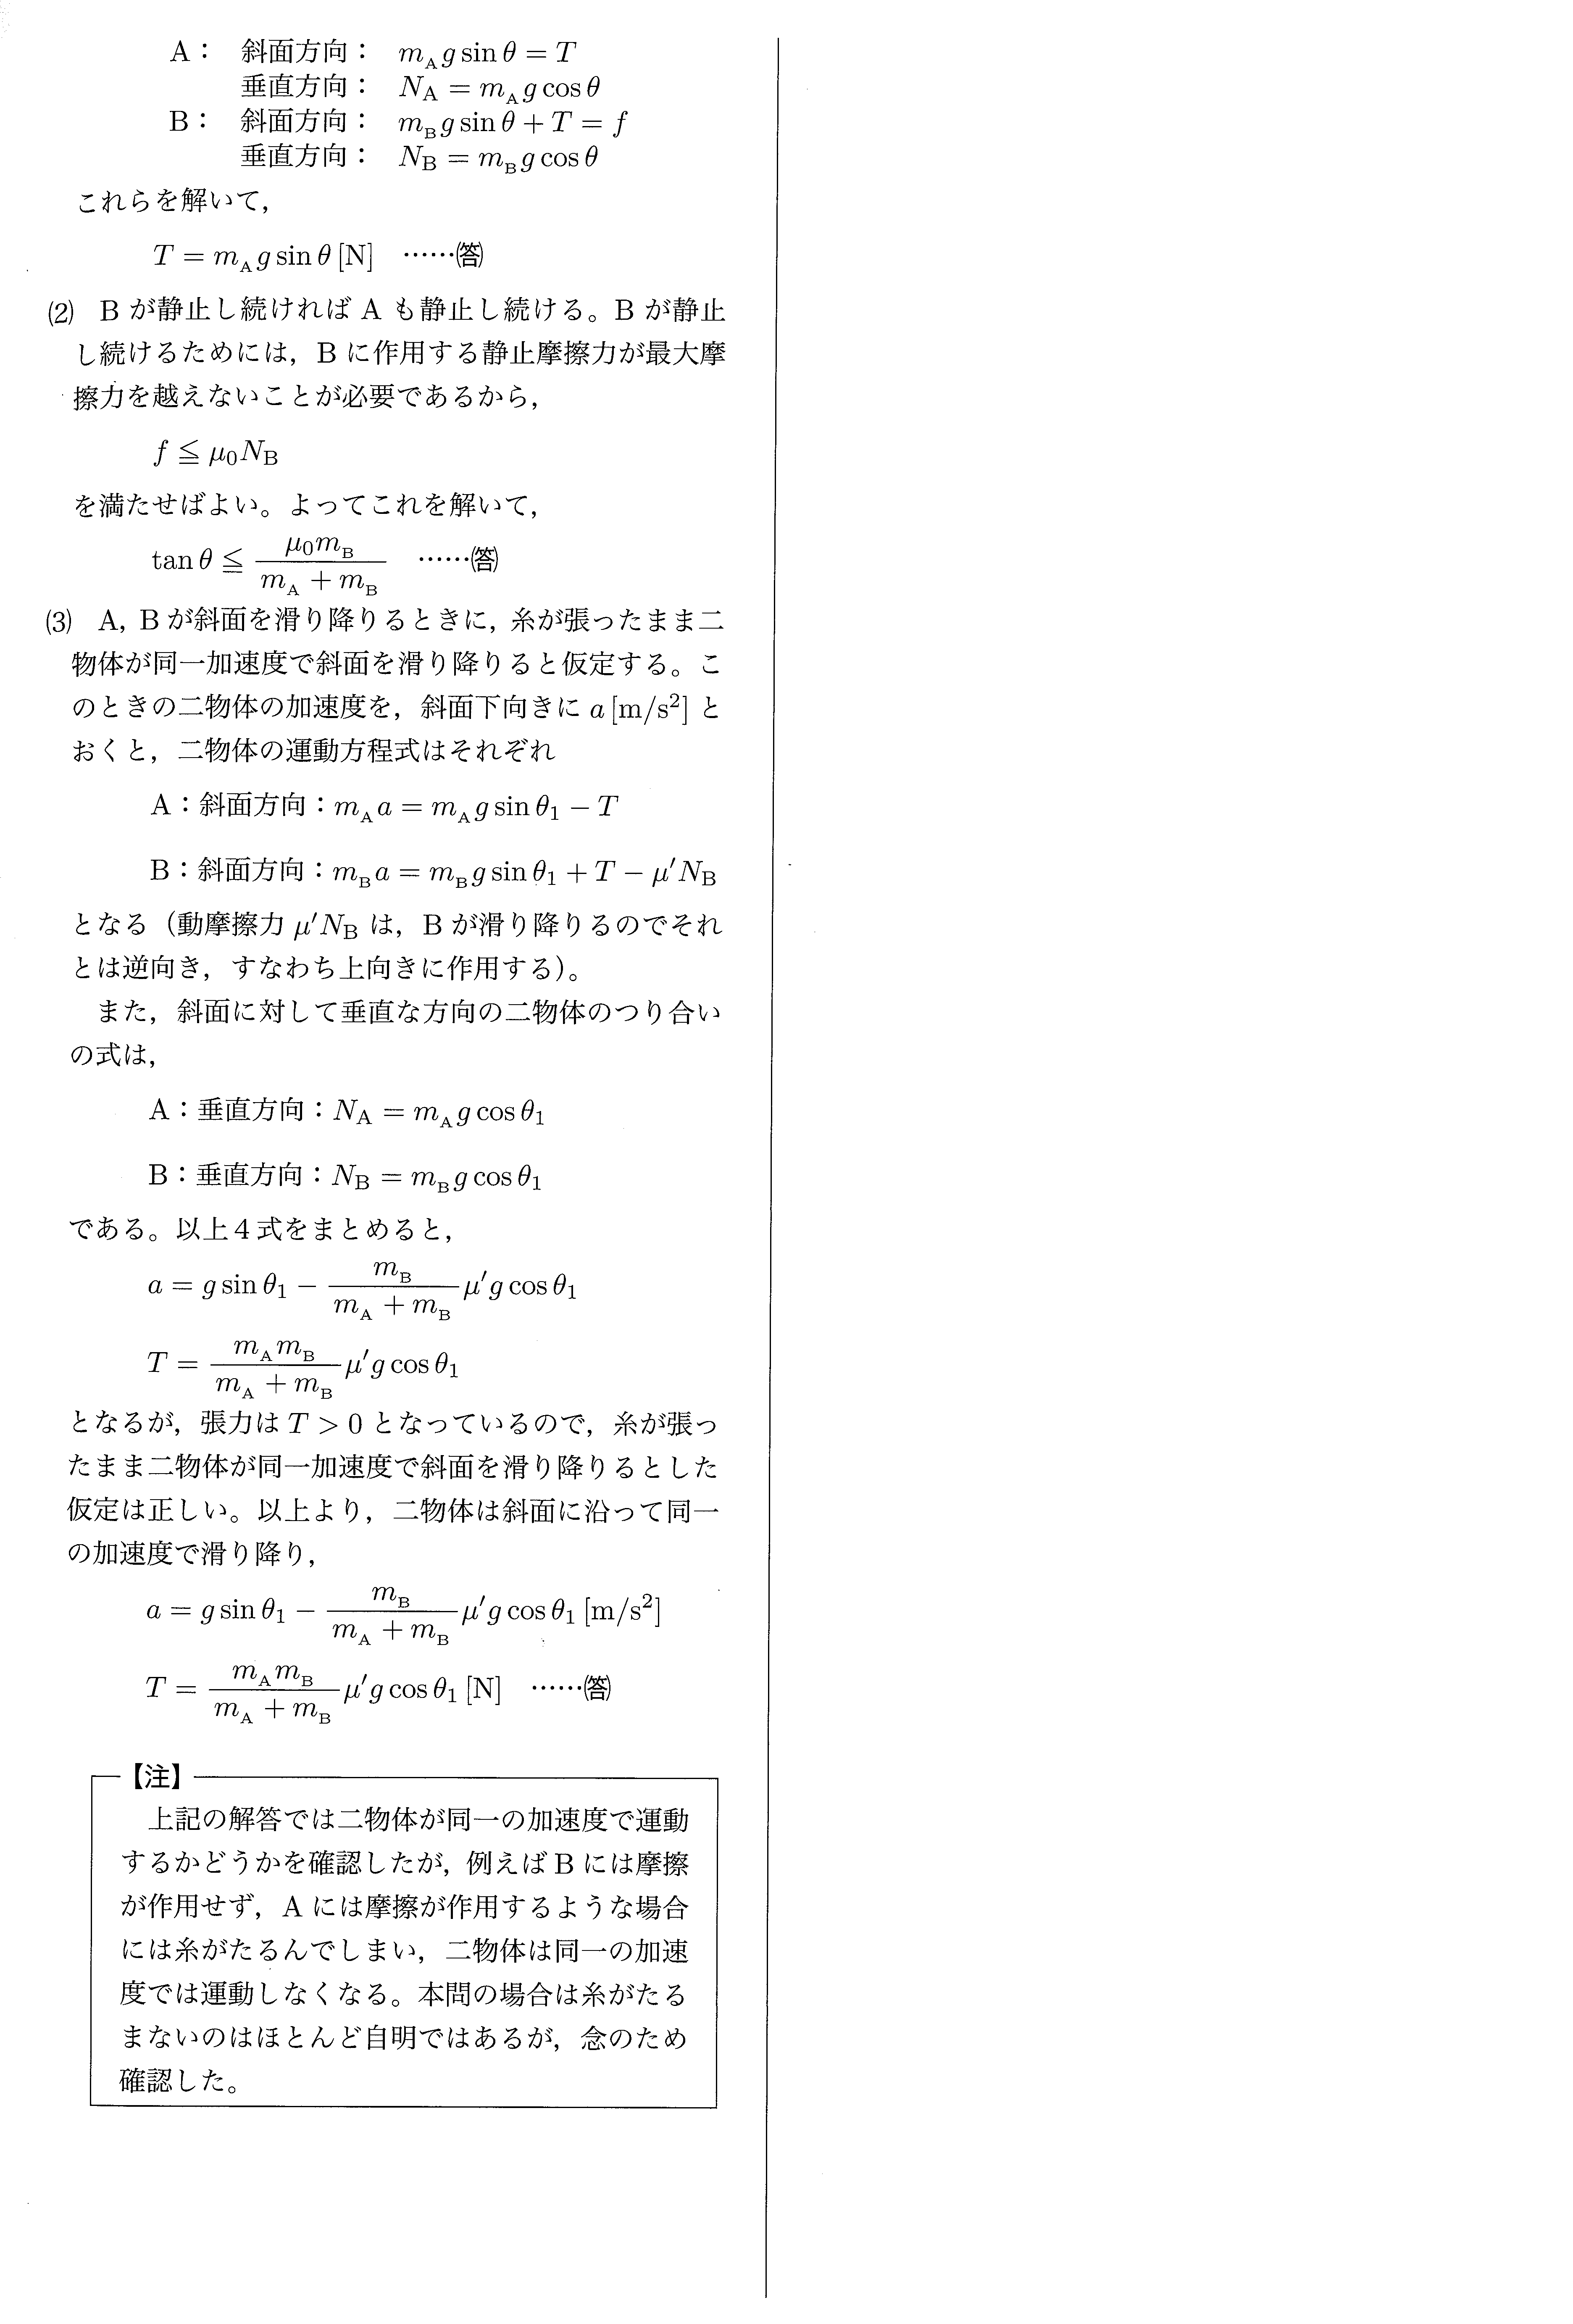
\includegraphics[width=170mm]{prob_p81_1.png}
\end{center}
\end{figure}













\include{physics_ch5}
\include{physics_ch6}
\section{物体の衝突と跳ね返り係数}

\subsection{跳ね返り係数}

\begin{wrapfigure}[10]{r}[5mm]{60mm}
  \centering
  \vspace{-5mm}
  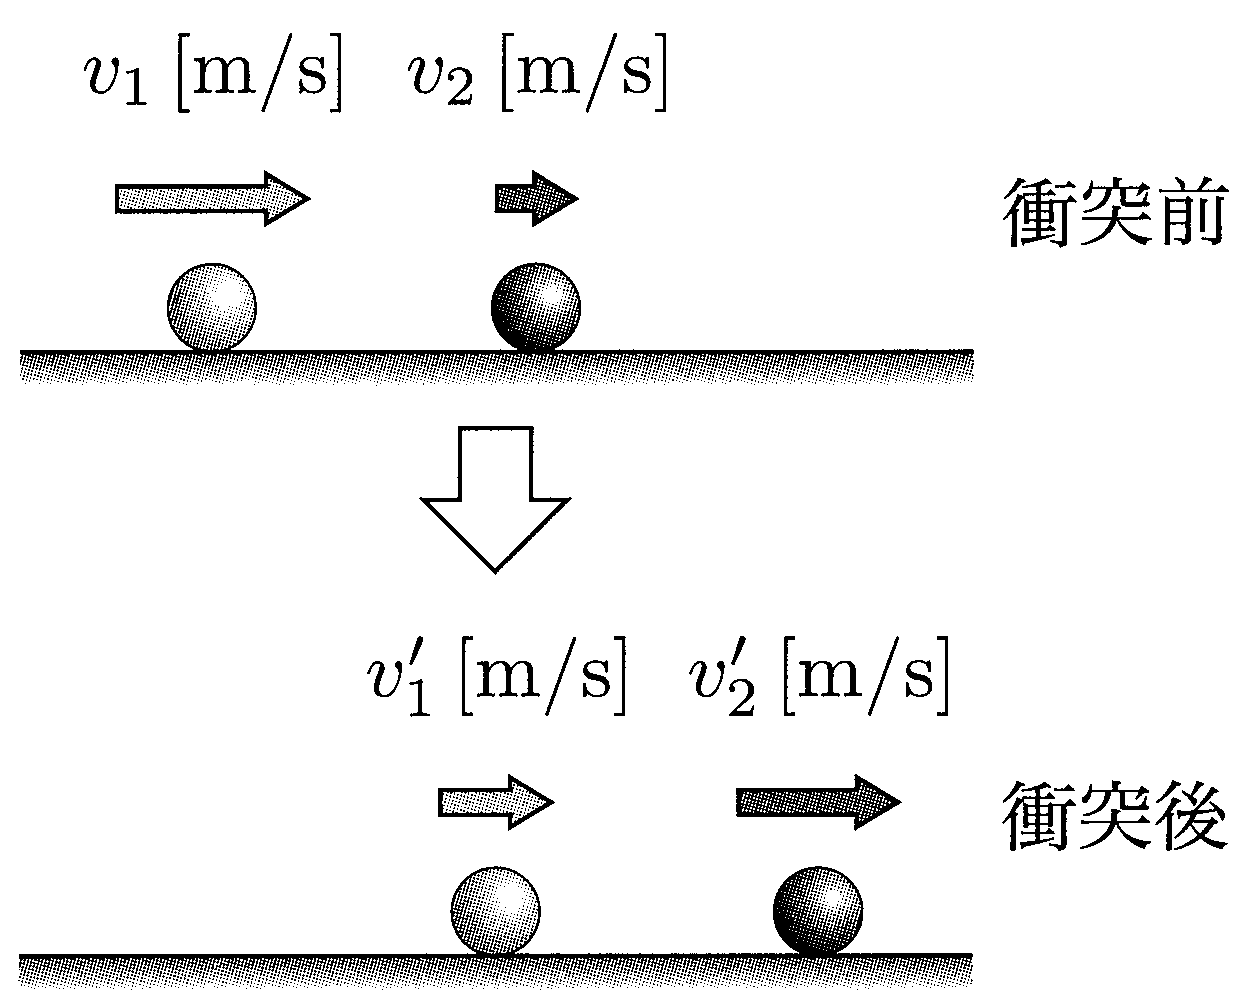
\includegraphics[keepaspectratio,width=60mm]
  {text_p33_fig1.png}
\end{wrapfigure}

摩擦のない床面の上を一直線上で運動する質量$m_1$[kg]の物体と質量$m_2$[kg]の物体とが，右向きを正として速度$v_1$[m/s]，$v_2$[m/s]で衝突し，その結果，速度が$v_1'$[m/s]および$v_2'$[m/s]になったとき，運動量保存則
\[ m_1v_1+m_2v_2=m_1v_1'+m_2v_2'\]
が成立する．
しかし，この式だけでは衝突後の2物体の速度$v_1',v_2'$を求めることは不可能である．
金属球同士の衝突と，粘土で作った球同士の衝突を比較すれば明らかなように，実際の衝突後の速度はこの運動量保存則と，2物体の材質・形状によって決まる．

実験によると，衝突直前の2物体の相対速度の大きさ（＝{\bf 相対的に近づく速さ}）と，衝突直後の2物体の相対速度の大きさ（＝{\bf 相対的に離れる速さ}）との比の値は，2物体によって決まる一定の値になることが知られている．
上図の場合，相対的に近づく速さは$v_1-v_2$，相対的に遠ざかる速さは$v_2'-v_1'$であり，
\[ e=\dfrac{（相対的に離れる速さ）}{（相対的に近づく速さ）}=\dfrac{v_2'-v_1'}{v_1-v_2} \]

この比の値$e$のことを，その2物体の{\bf 跳ね返り係数}という．

また，衝突に際して，相対速度の向きは必ず反転するので，衝突前後の相対速度$v_1-v_2$と$v_1'-v_2'$を用いれば
\[ e=-\dfrac{（衝突直後の相対速度）}{（衝突直前の相対速度）}=-\dfrac{v_1'-v_2'}{v_1-v_2}\]
と表されることになる．

必ず離れる速さは近づく速さ以下になる．
そのため，\mbox{\boldmath $跳ね返り係数eは0\leqq e \leqq 1 の範囲の正の値となる$}．

\begin{matome}{跳ね返り係数}
 \hspace{5mm} 跳ね返り係数\hspace {10mm}$e=\dfrac{（相対的に離れる速さ）}{（相対的に近づく速さ）}=-\dfrac{（衝突直後の相対速度）}{（衝突直前の相対速度）}$
 \end{matome}
 
  \ 
%  
%\begin{breakbox}
%\ex＜跳ね返り係数による衝突の分類＞\\
%\begin{wrapfigure}[7]{r}[5mm]{50mm}
%  \centering
%  \vspace{-5mm}
%  \includegraphics[keepaspectratio,width=40mm]
%  {text_p33_fig2.png}
%\end{wrapfigure}
%\hspace{5mm}水平でなめらかな床面の上に，質量$M$[kg]の物体Bが静止して置かれている．
%これに質量$m$[kg]の物体Aを速さ$v_0$[m/s]で衝突させる場合について以下の問いに答えよ．
%ただし，A,Bの間の跳ね返り係数は$e$であり，物体Aの初速度の向きを速度の正の向きとする．
%\begin{description}
%\item[(1)] 衝突後の物体A,Bの速度をそれぞれ$v$[m/s]，$V$[m/s]とする．このとき，運動量保存則および跳ね返り係数の式を立てよ．
%\item[(2)] 衝突後の物体A,Bの速度$v,V$をそれぞれ求めよ．
%\item[(3)] この衝突による運動エネルギーの減少量を求めよ．
%\item[(4)] 運動エネルギーの減少がないときの跳ね返り係数の値，および減少量が最も大きくなるときの跳ね返り係数の値をそれぞれ求めよ．
%\end{description}
%
%\end{breakbox}

% \newpage
跳ね返り係数$e$に応じて衝突は以下のように分類される．

 \begin{matome}{跳ね返り係数による衝突の分類}
 \hspace{5mm} \MARU{1} \hspace{2mm}\mbox{\boldmath $e=1$} \hspace {11mm}{\bf 弾性衝突（完全弾性衝突）}\\
 \hspace{10mm} 衝突前後で全運動量と同時に全力学的エネルギーも保存される．\\
 \hspace{5mm} \MARU{2} \hspace{2mm}\mbox{\boldmath $0<e<1$}\hspace {5mm}{\bf 非弾性衝突}\\
 \hspace{10mm} 力学的エネルギーの一部が衝突により，音，発熱，変形などによって失われる．\\
 \hspace{5mm} \MARU{3} \hspace{2mm}\mbox{\boldmath $e=o$}\hspace {13mm}{\bf 完全非弾性衝突}\\
 \hspace{10mm} 2物体は合体する．力学的エネルギーの損失が最大となる．
 \end{matome}


\subsection{壁面・床面との垂直な衝突による跳ね返り}

今ままでは2物体間の衝突を考えてきたが，壁面や床面と物体が衝突して跳ね返るときは壁や床の質量をはっきりさせることができないため，運動量保存則を用いることができない．
しかし，壁面や床面は通常，物体に比べて質量が非常に大きく，静止したままであることが多い．
このような場合は物体と壁面・床面との間の跳ね返り係数$e$を用いて跳ね返りを考えることができる．

 \ 
 
%\begin{breakbox}
%\ex＜床面との垂直衝突＞\\
%\begin{wrapfigure}[7]{r}[5mm]{70mm}
%  \centering
%  \vspace{-5mm}
%  \includegraphics[keepaspectratio,width=60mm]
%  {text_p34_fig1.png}
%\end{wrapfigure}
%\hspace{5mm}質量$m$[kg]の小球を，床面から高さ$h$[m]のところから自由落下させ，床面でバウンドさせる．
%床面と小球との間の跳ね返り係数は$e\hspace{2mm}(0<e<1)$である．
%重力加速度の大きさを$g {\rm [m/s^2]}$として以下の問いに答えよ．
%\begin{description}
%\item[(1)] 最初に床面に衝突する直前の速さ$v_0$[m/s]を求めよ．
%\item[(2)] 1回目のバウンドの直後，小球が跳ね上がる速さ$v_1$[m/s]を求めよ．
%\item[(3)] 1回目のバウンドの後，小球の達する最高点の高さ$h_1$[m]を求めよ．
%\item[(4)] 2回目のバウンドの後，小球の達する最高点の高さ$h_2$[m]を求めよ．
%\item[(5)] 小球が飛び跳ねなくなるまでに要する時間$T$[s]を求めよ．
%\end{description}
%
%\end{breakbox}

% \newpage 
  

\subsection{壁面・床面との斜めの衝突による跳ね返り}

\begin{wrapfigure}[10]{r}[5mm]{70mm}
  \centering
  \vspace{-5mm}
  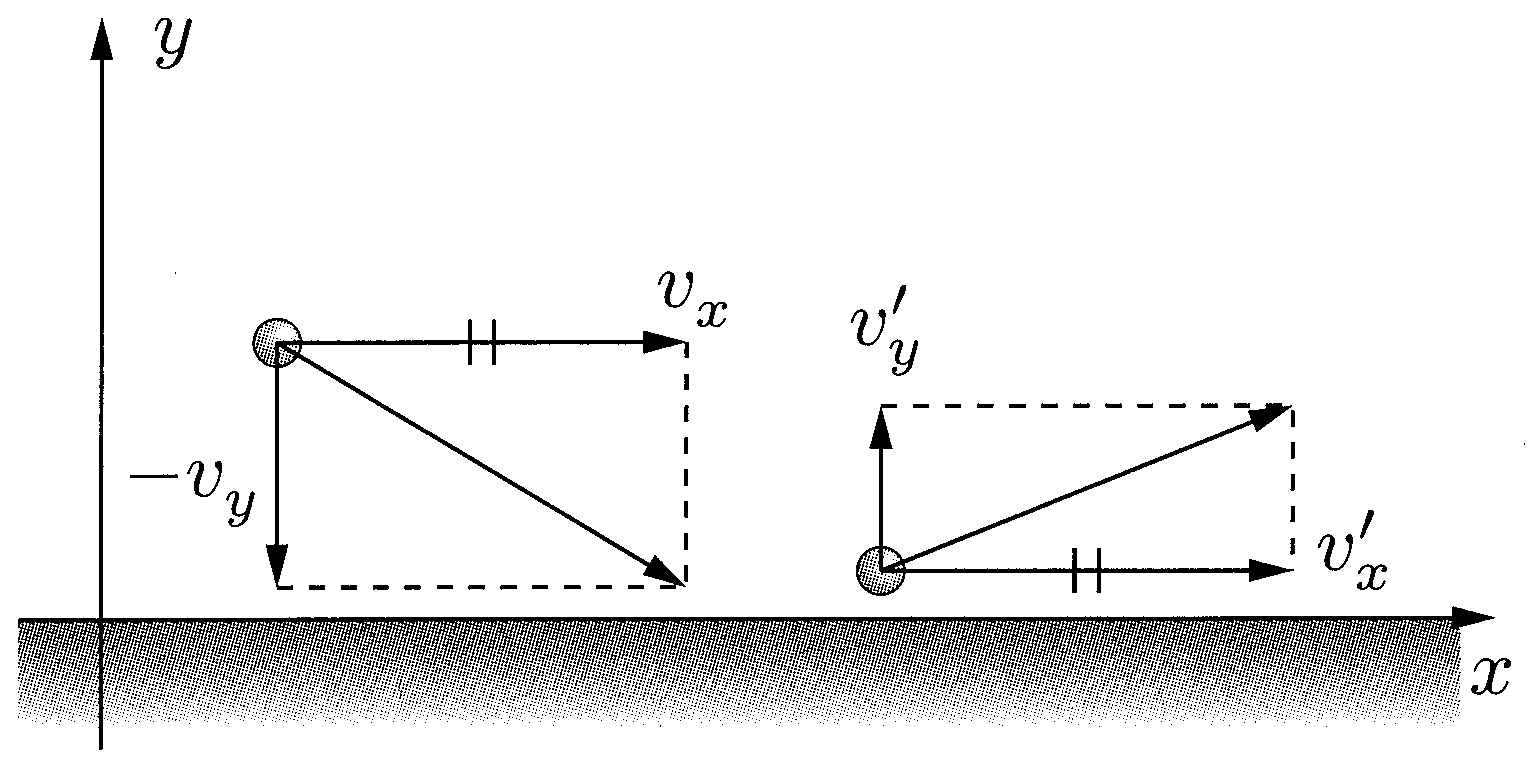
\includegraphics[keepaspectratio,width=70mm]
  {text_p35_fig1.png}
\end{wrapfigure}

物体が壁面や床面に対して斜めに衝突するとき，摩擦が無視できる場合には{\bf 接触面に平行な速度成分は衝突によって変化しない．}
一方，{\bf 接触面に垂直な速度成分は跳ね返り係数}\mbox{\boldmath $eによって速さが変化する．$}
右図のように軸を取り，衝突前後の物体の速度をそれぞれ$(v_x,v_y)$および$(v_x',v_y')$とすると（衝突前の$y$軸成分は負の値となる），
\[ v_x'=v_x ,\hspace{3mm} e=-\dfrac{v_y'}{v_y} \]
が成立する．

% \ 
% 
%\begin{breakbox}
%\ex＜壁面・床面との斜めの衝突による跳ね返り＞\\
%\begin{wrapfigure}[7]{r}[5mm]{60mm}
%  \centering
%  \vspace{-5mm}
%  \includegraphics[keepaspectratio,width=50mm]
%  {text_p35_fig2.png}
%\end{wrapfigure}
%\hspace{5mm}質量$m$[kg]の小球を，図のように水平な床面上の点Aから迎角$\theta$，初速$V_0$[m/s]で打ち出したところ，小球は距離$R$[m]離れたなめらかな鉛直な壁面にB点で衝突し，上向きに跳ね返った．
%小球と壁面との跳ね返り係数を$e$，重力加速度の大きさを$g {\rm [m/s^2]}$，速度は図の右向きおよび上向きを正の値にとるものとして以下の問いに答えよ．
%\begin{description}
%\item[(1)] 小球が壁面と衝突する直前の鉛直方向の速度を求めよ．
%\item[(2)] 小球が壁面と衝突した直後の水平方向の速度を求めよ．
%\item[(3)] 小球が壁面と衝突してから，最高点Cに達するまでの時間を求めよ．
%\item[(4)] 小球が床に落下する点Dと，壁面との距離$L$[m]を求めよ．
%\end{description}
%
%\end{breakbox}

\newpage

\begin{figure}[h]
\begin{center}
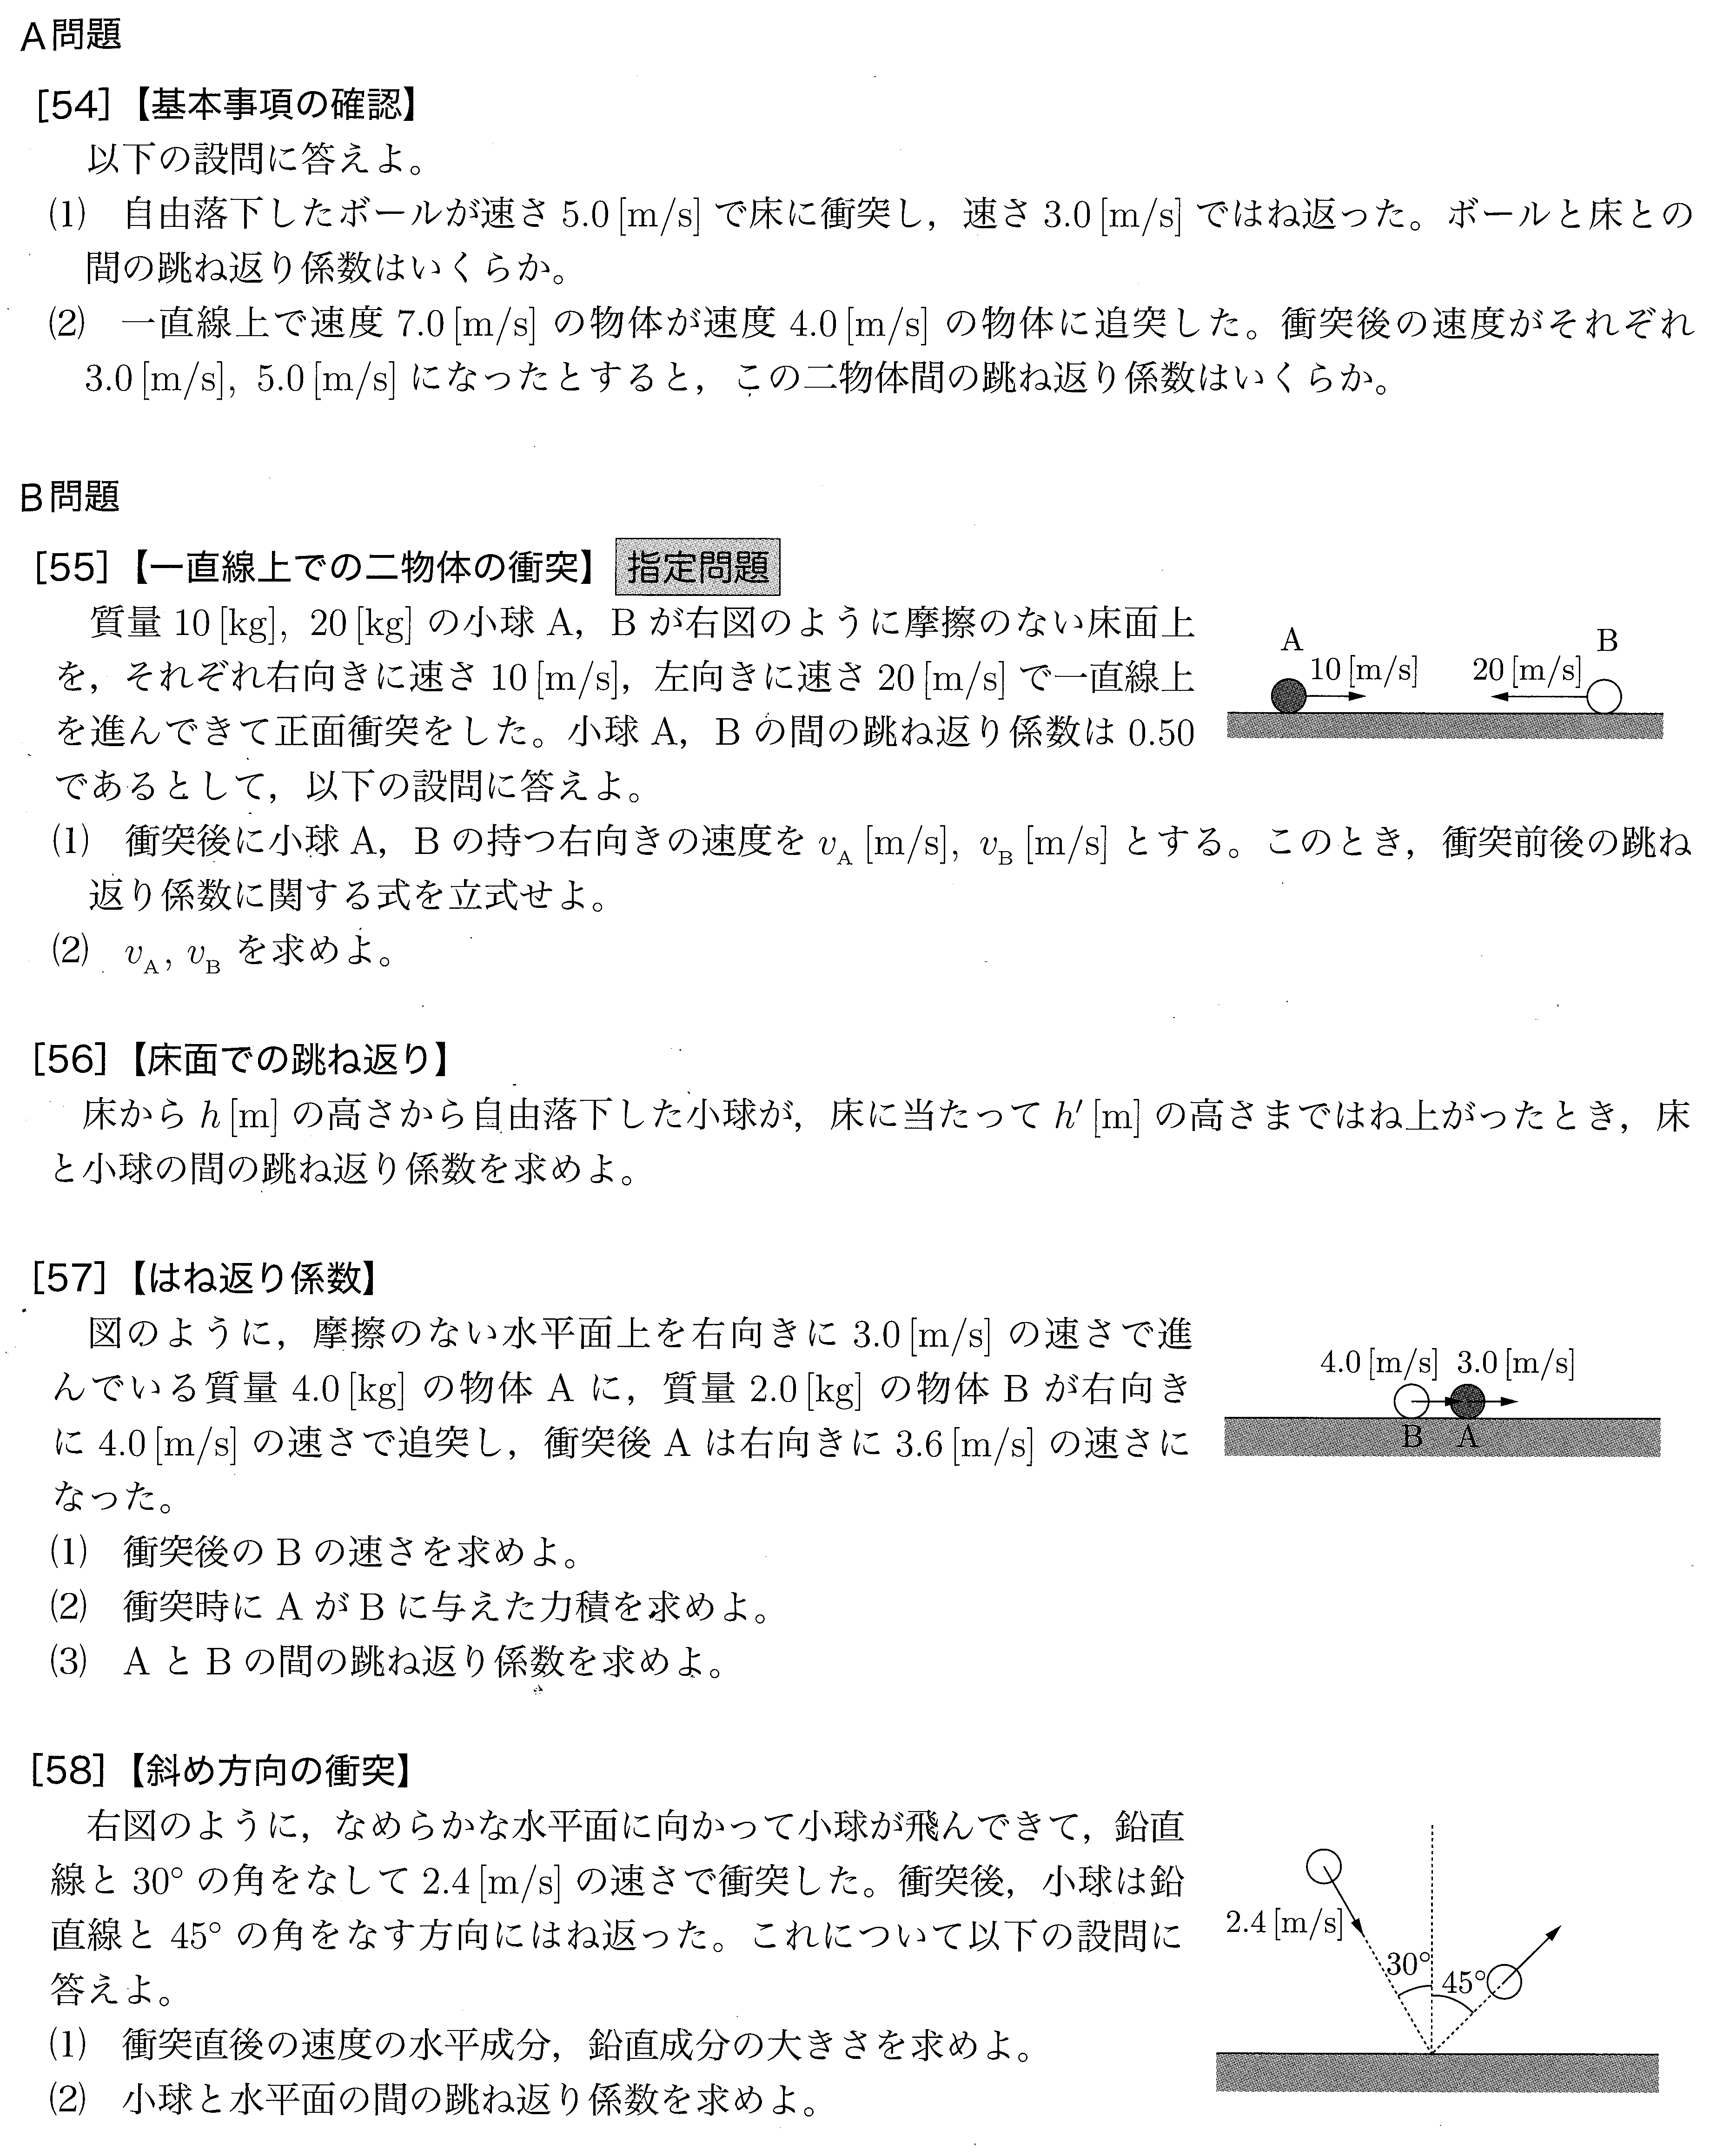
\includegraphics[width=170mm]{prob_p19.png}
\end{center}
\end{figure}

\newpage

\begin{figure}[h]
\begin{center}
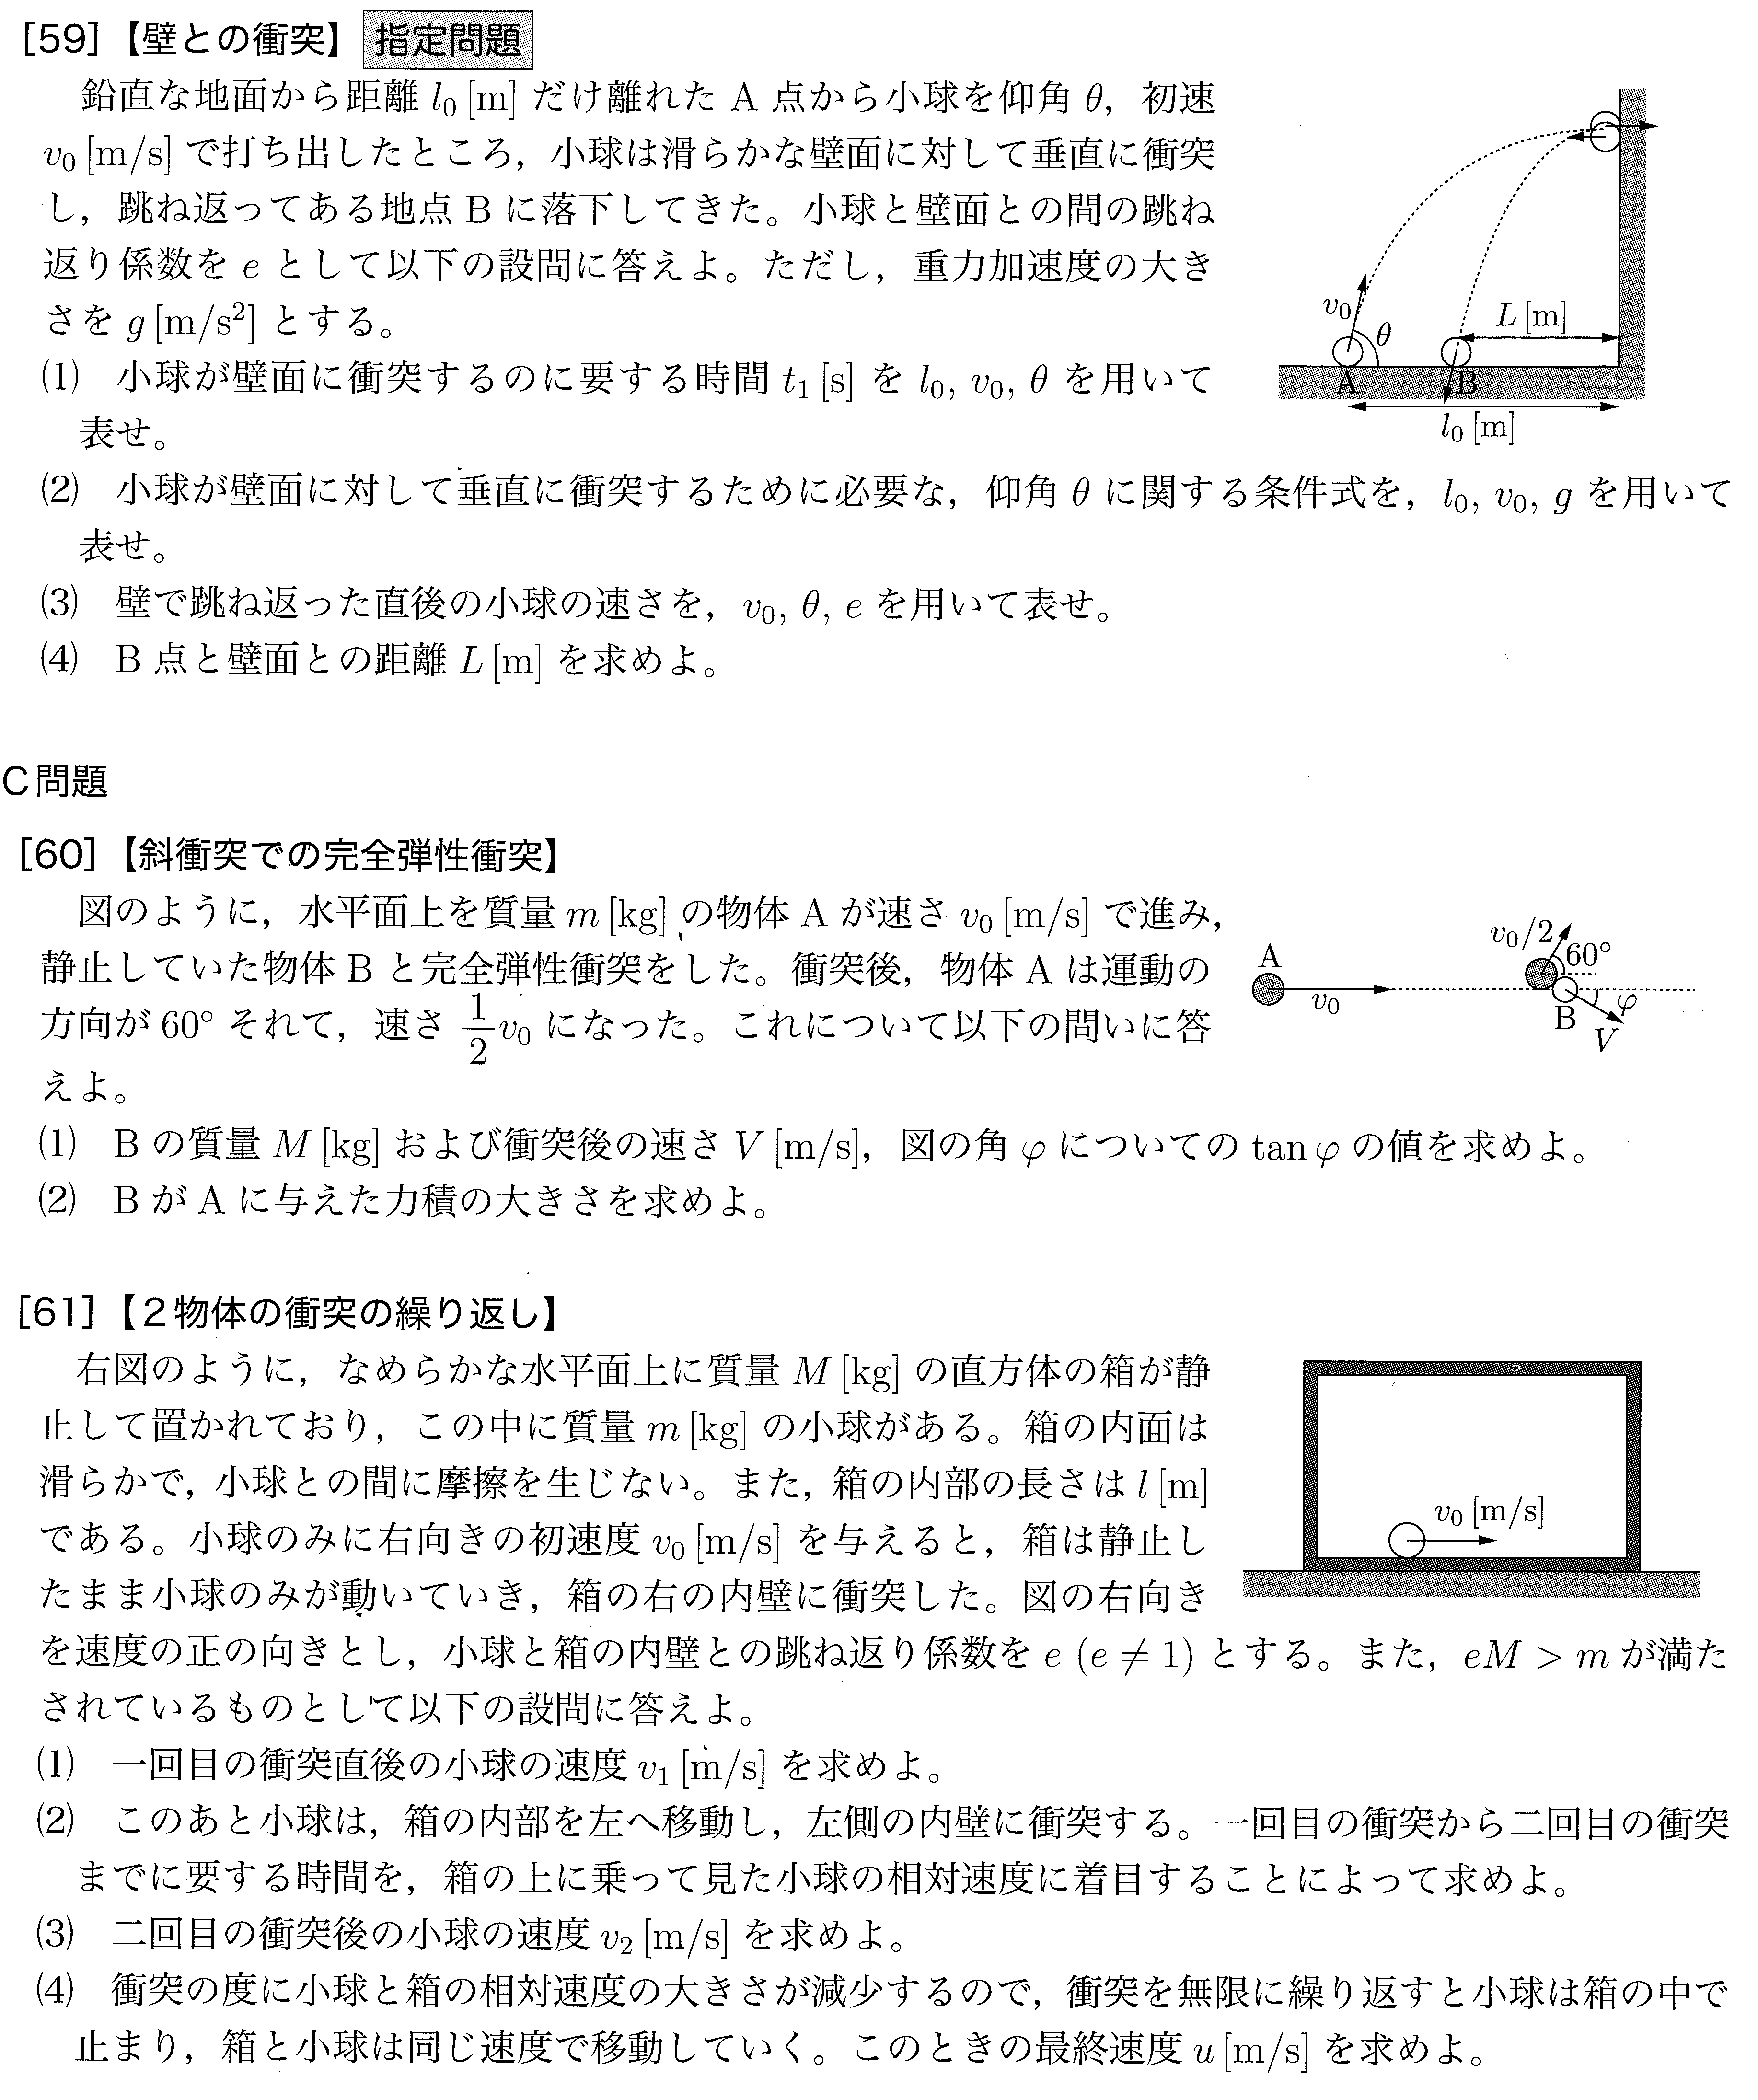
\includegraphics[width=170mm]{prob_p20.png}
\end{center}
\end{figure}



\newpage

\begin{figure}[h]
\begin{center}
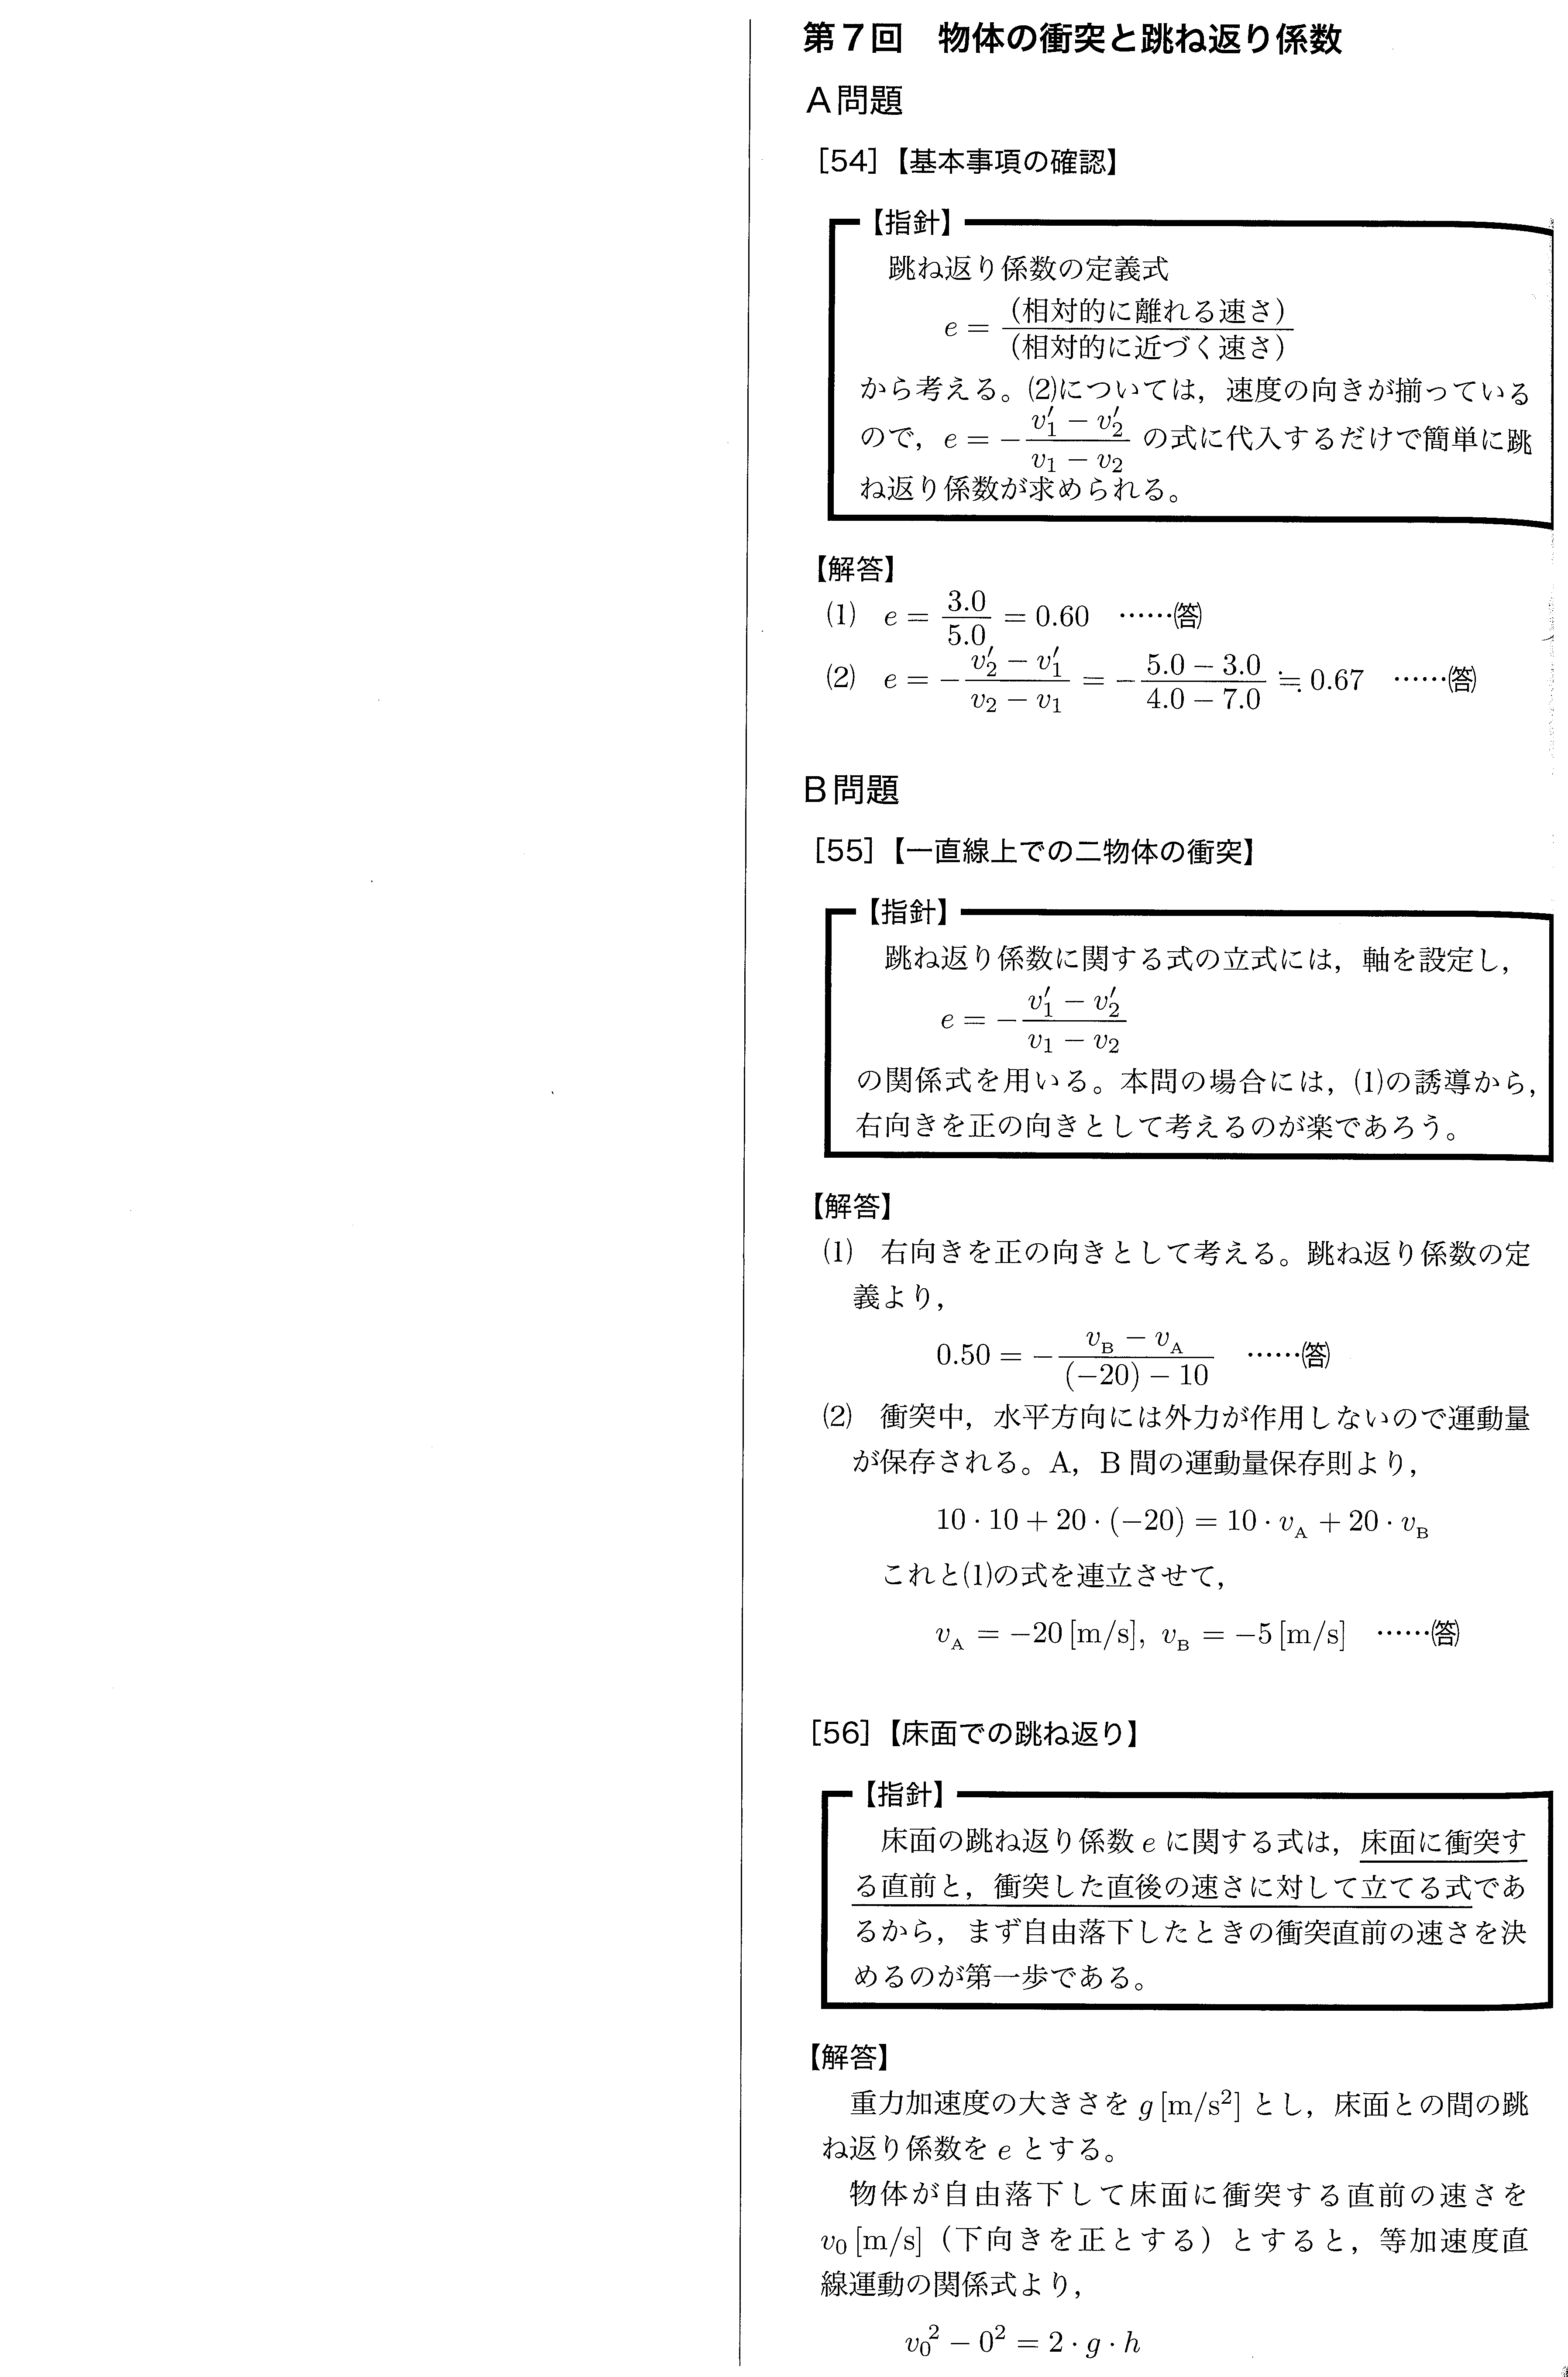
\includegraphics[width=170mm]{prob_p88_2.png}
\end{center}
\end{figure}

\newpage

\begin{figure}[h]
\begin{center}
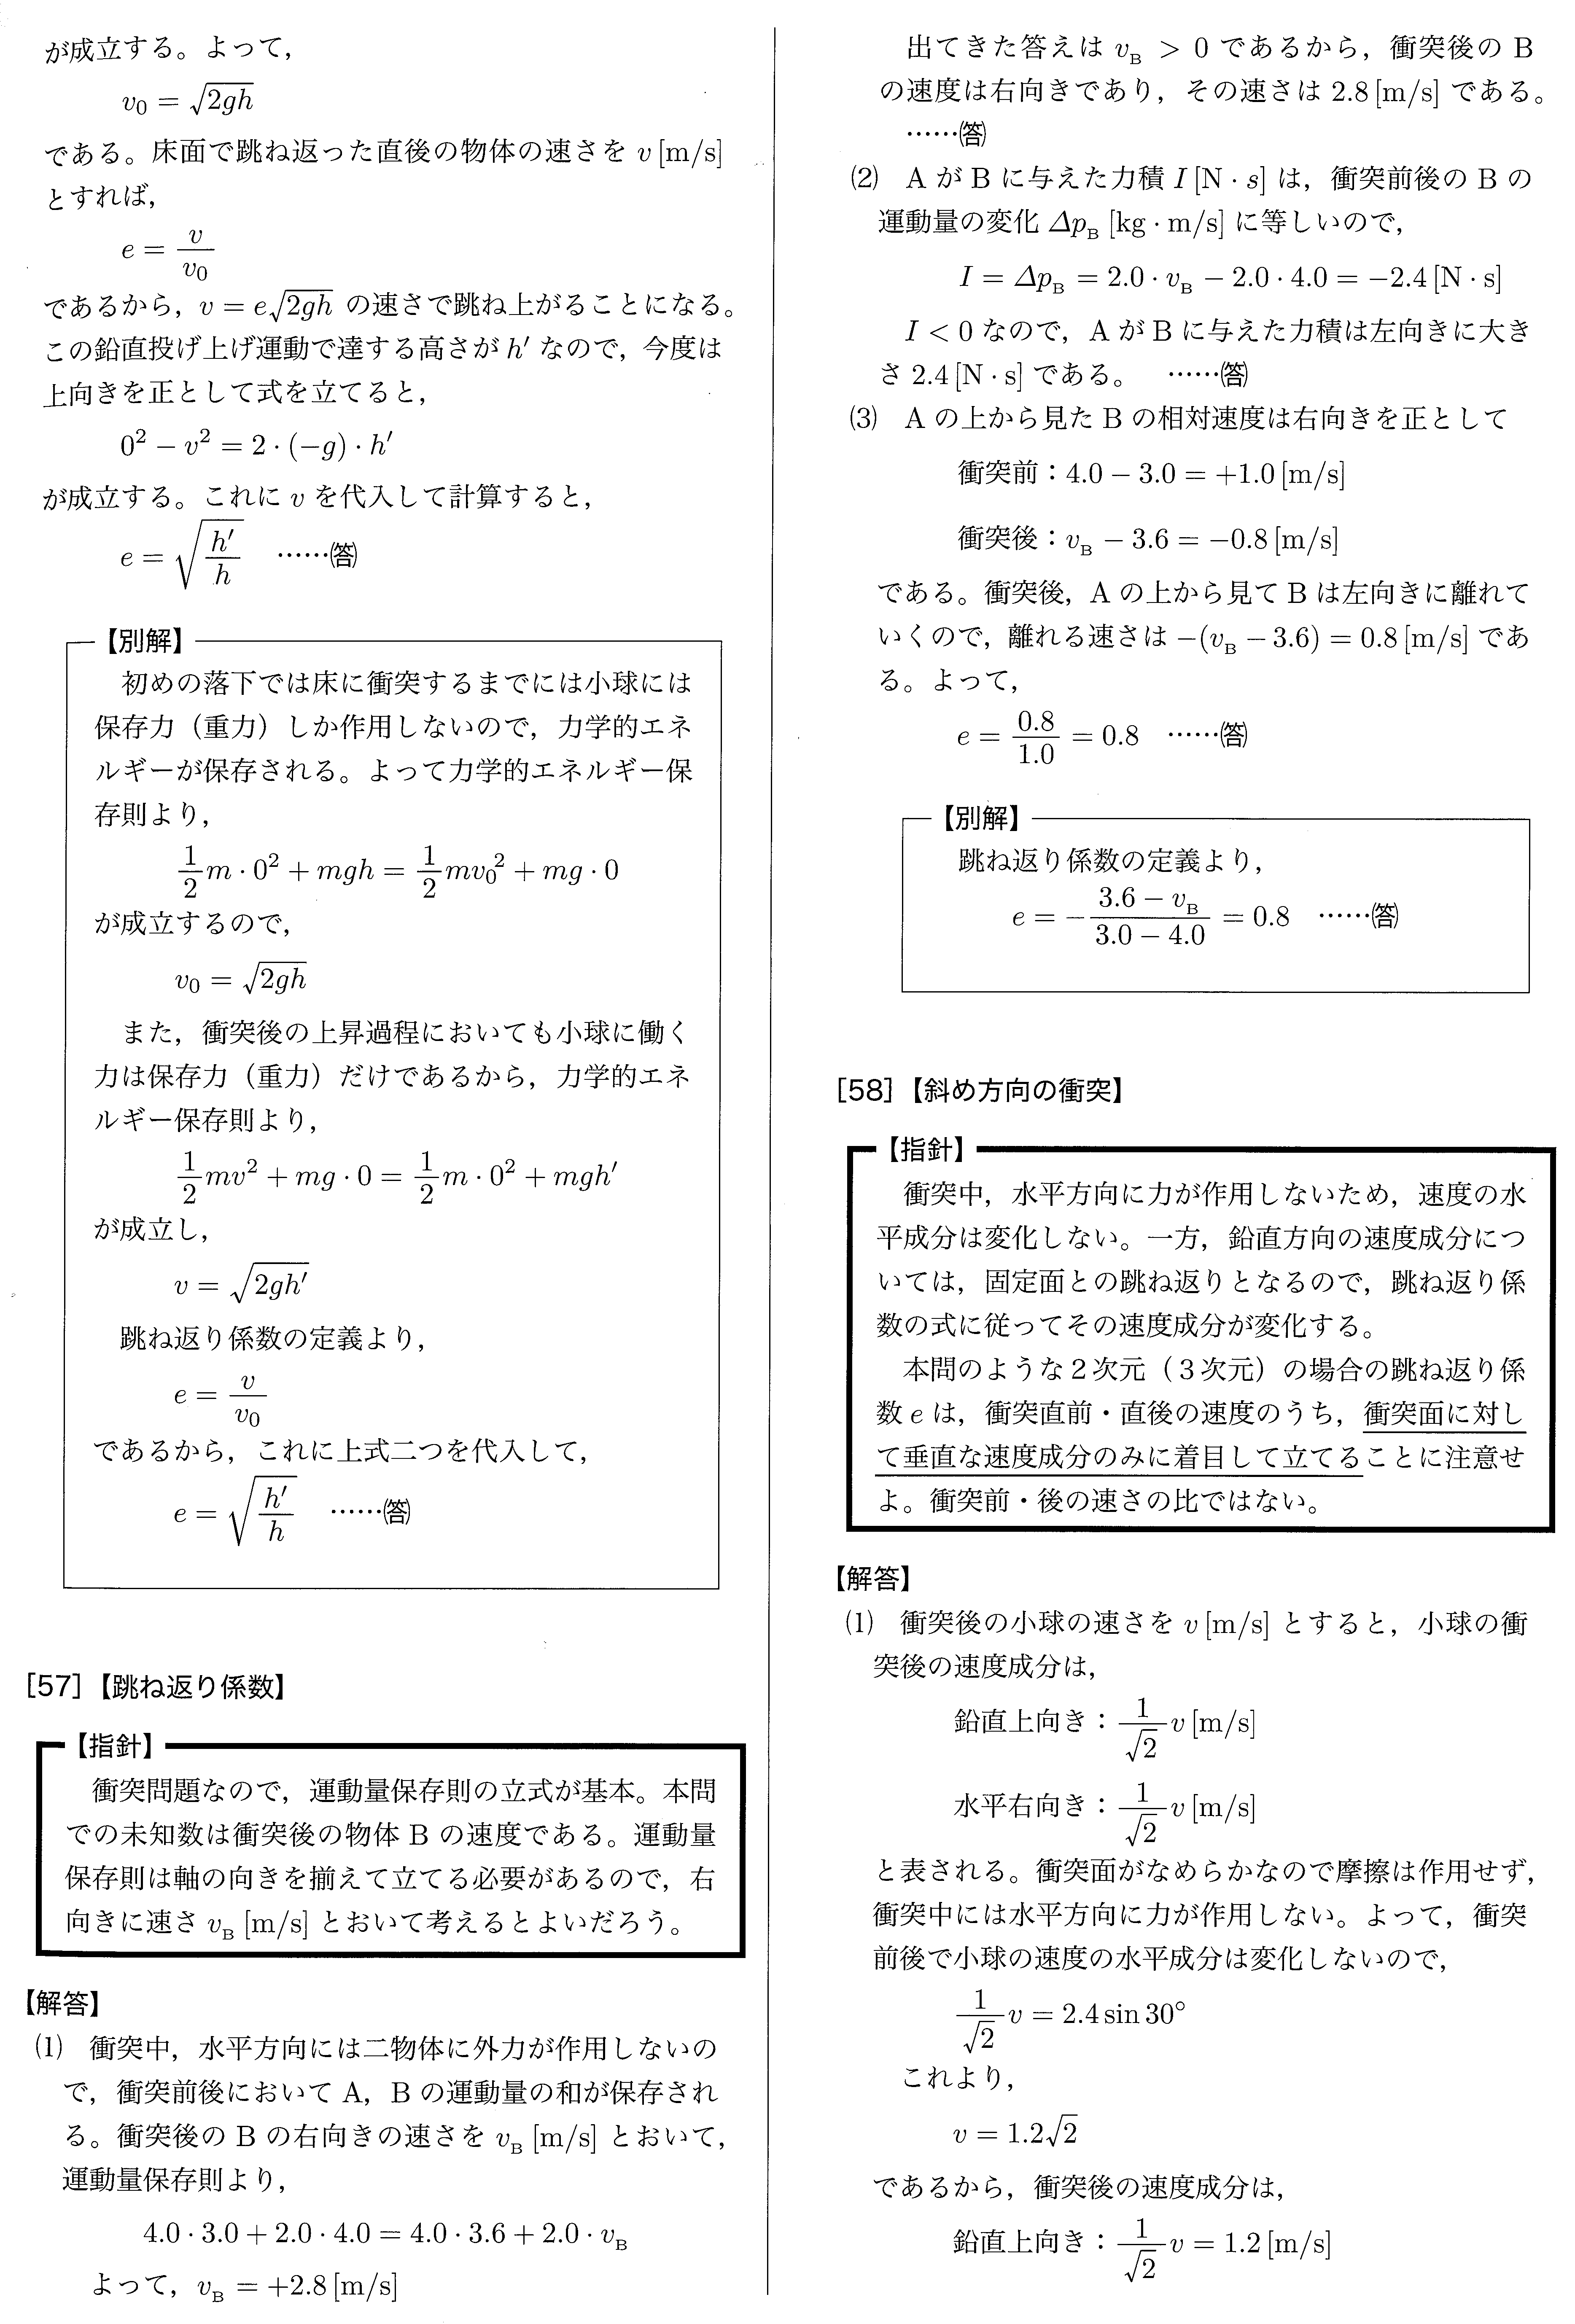
\includegraphics[width=170mm]{prob_p89.png}
\end{center}
\end{figure}

\newpage

\begin{figure}[h]
\begin{center}
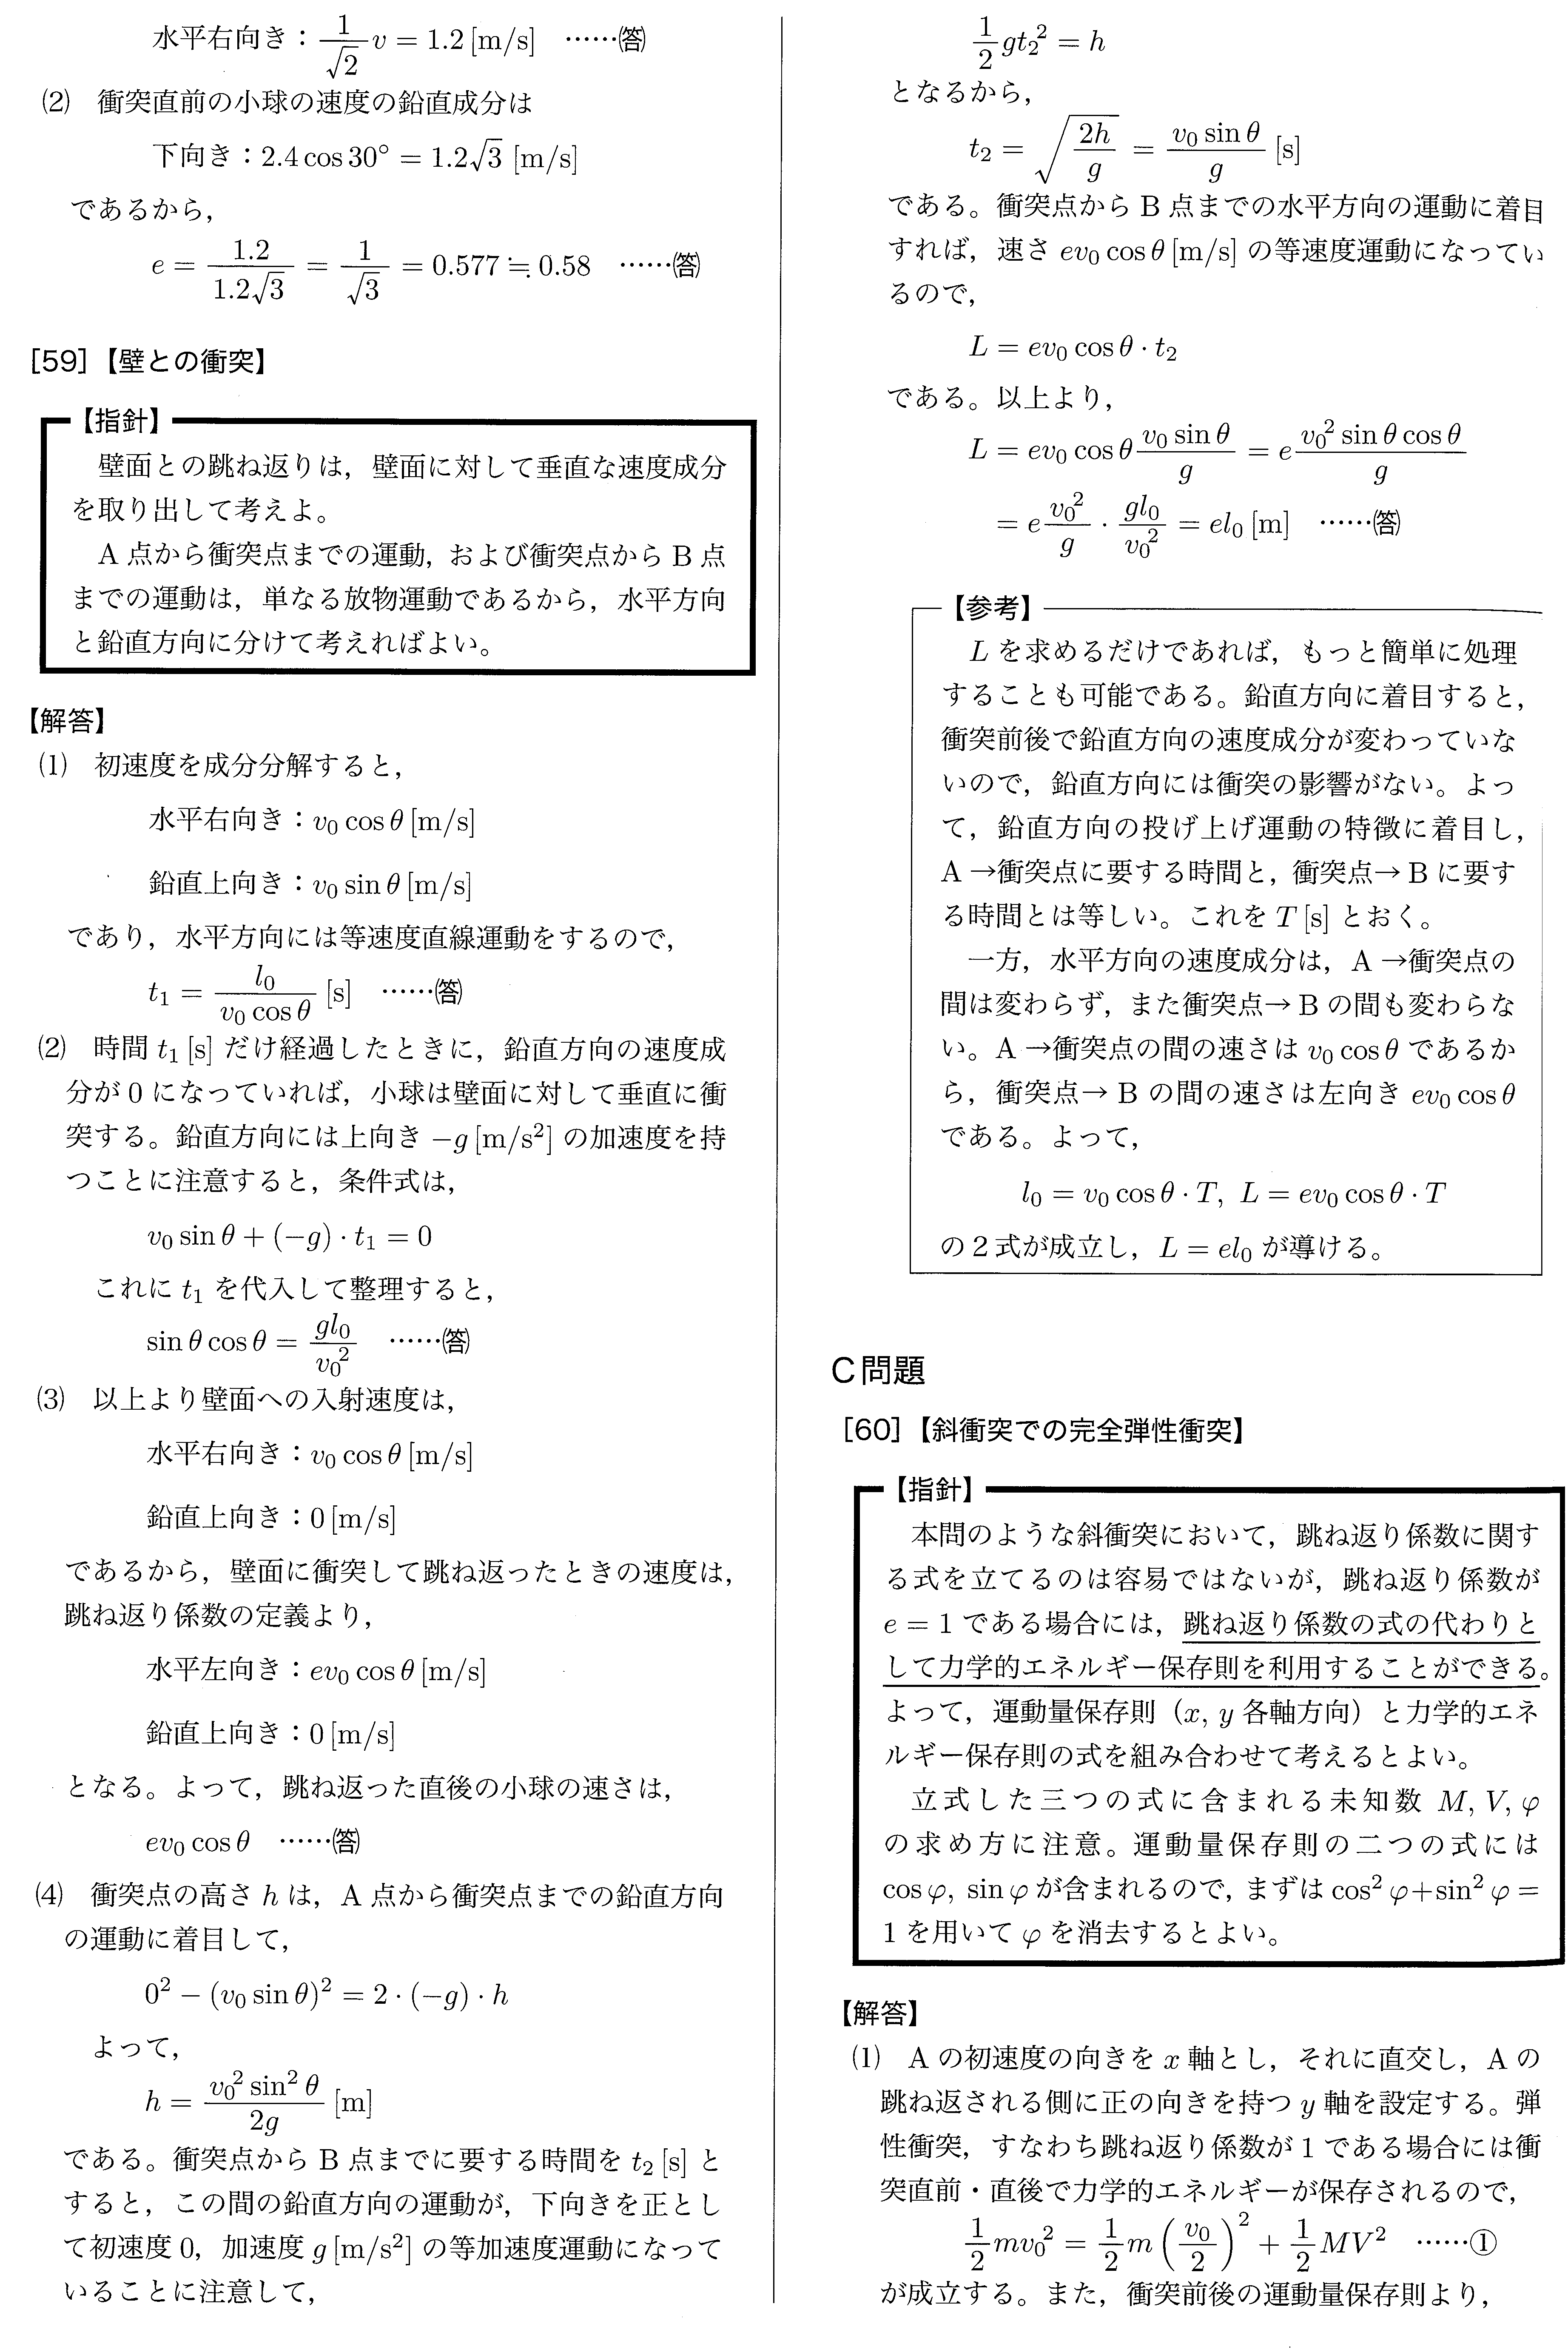
\includegraphics[width=170mm]{prob_p90.png}
\end{center}
\end{figure}

\newpage

\begin{figure}[h]
\begin{center}
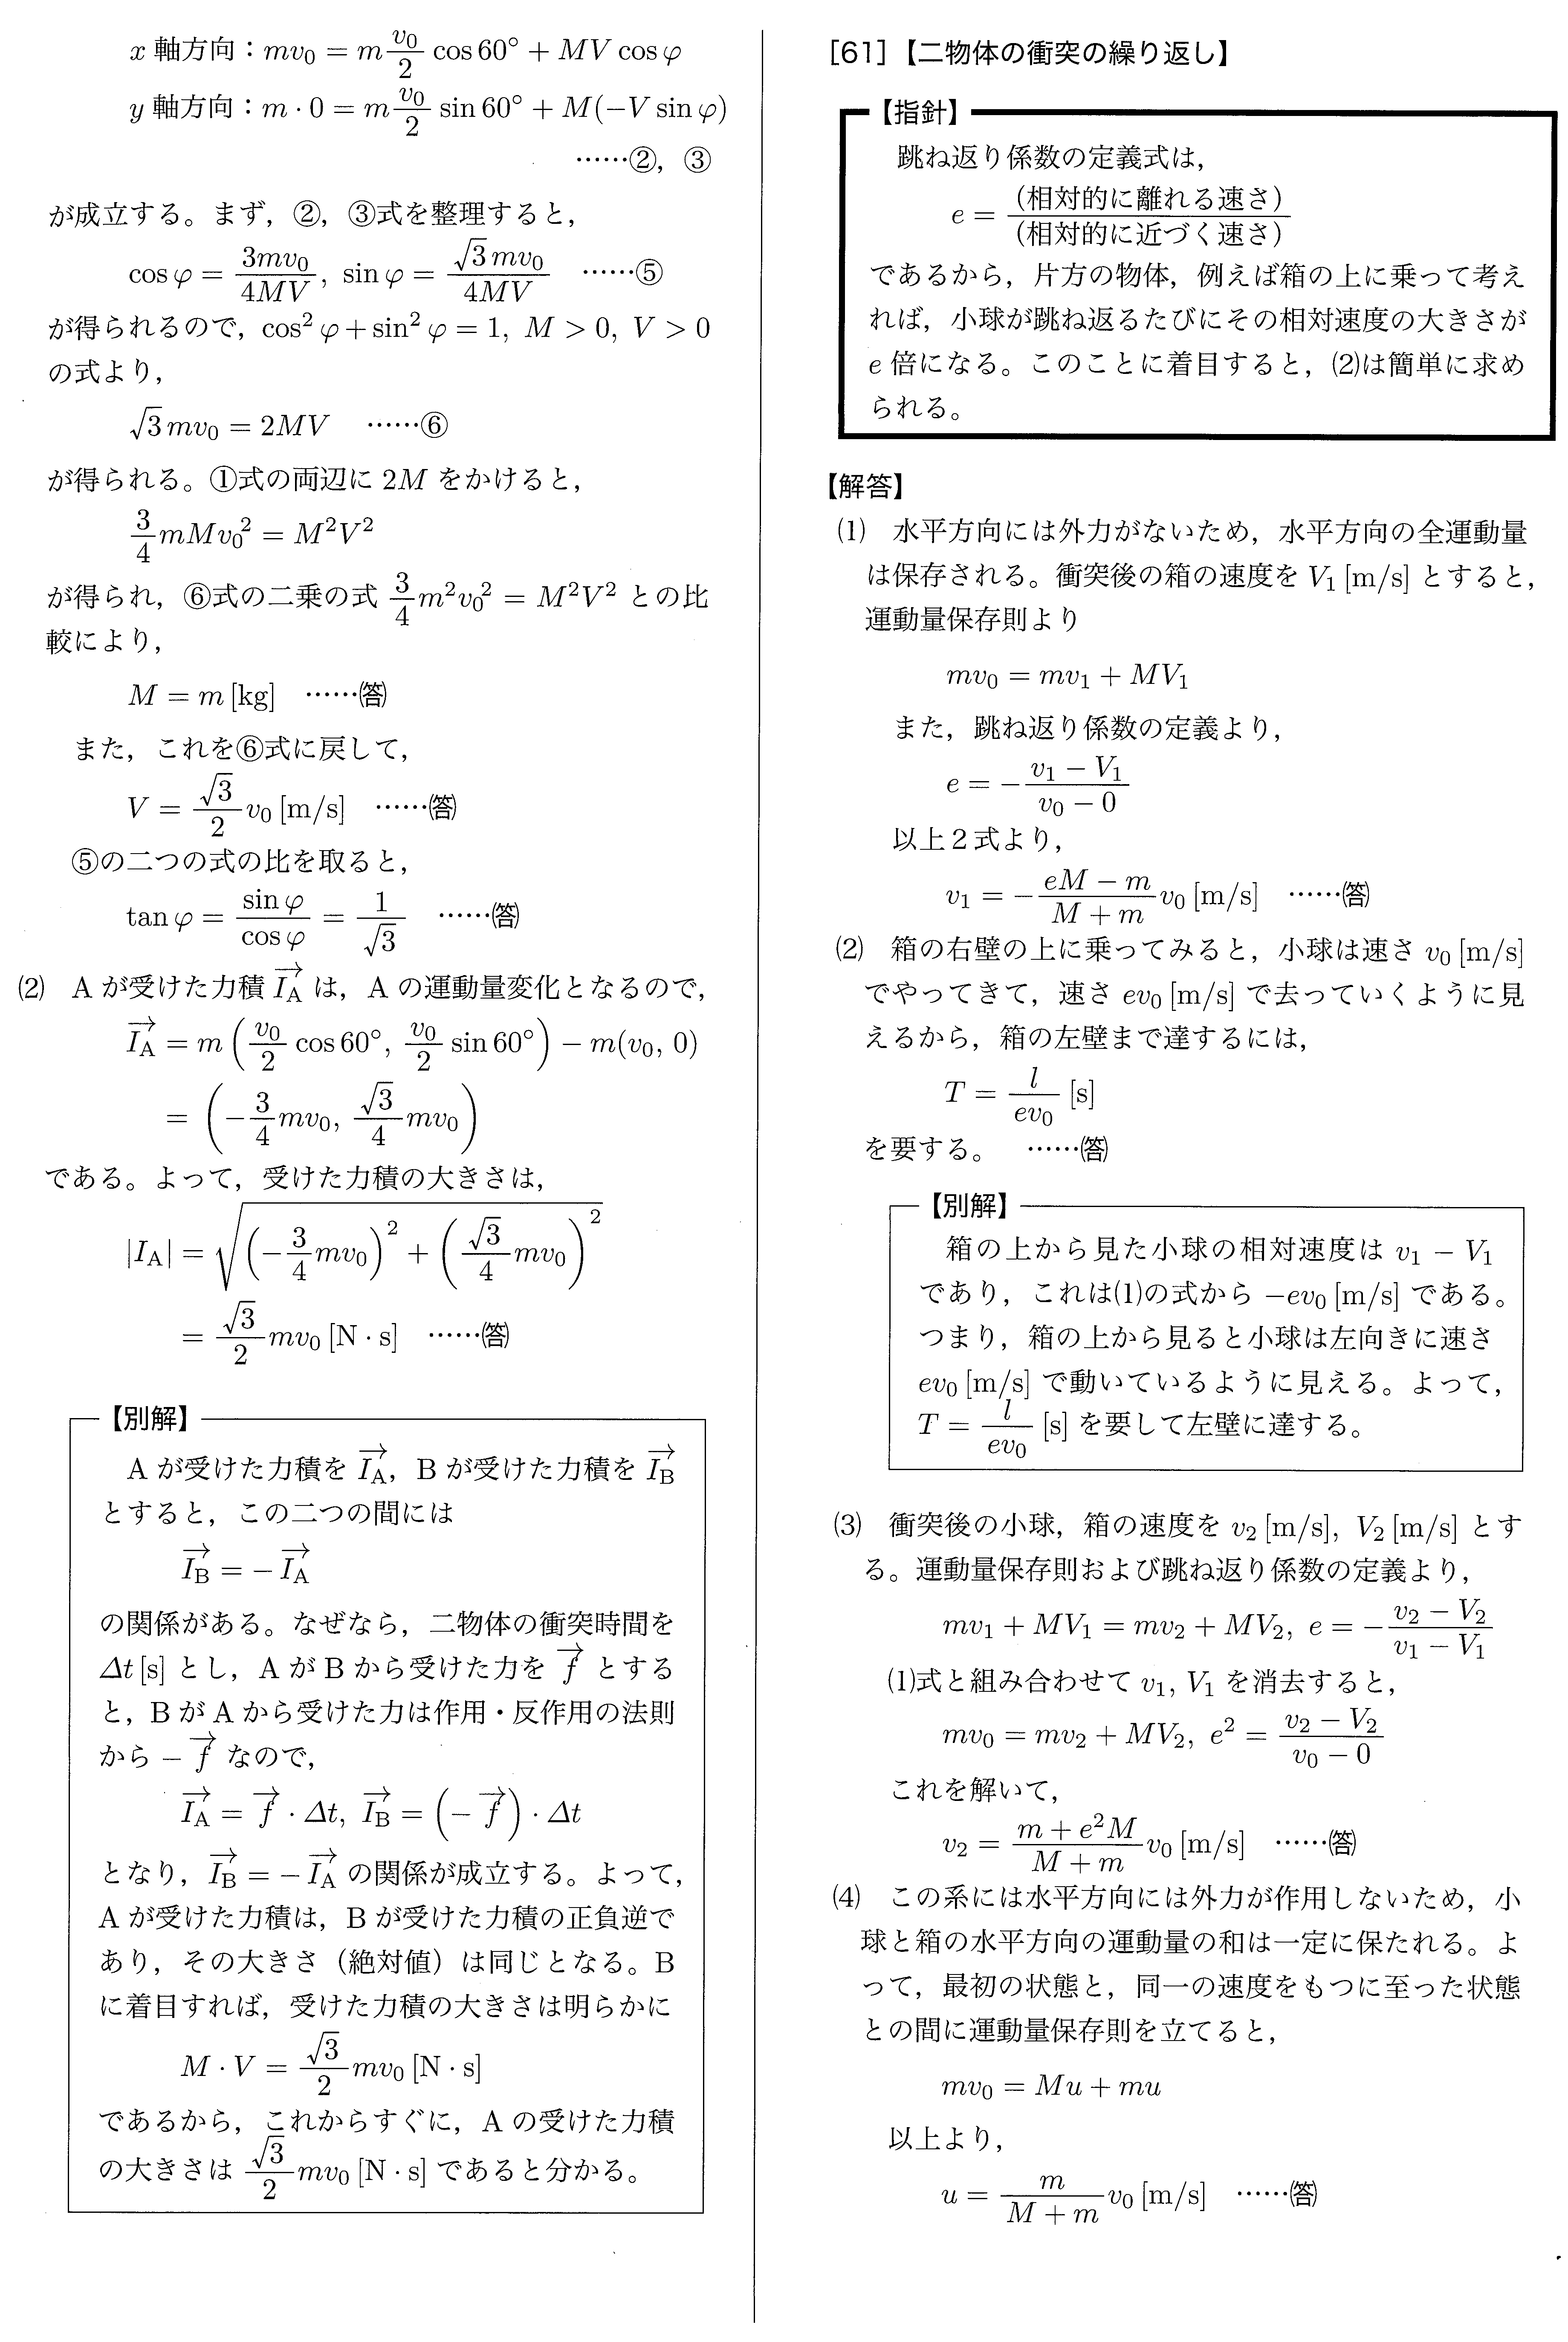
\includegraphics[width=170mm]{prob_p91.png}
\end{center}
\end{figure}

\newpage

\begin{figure}[h]
\begin{center}
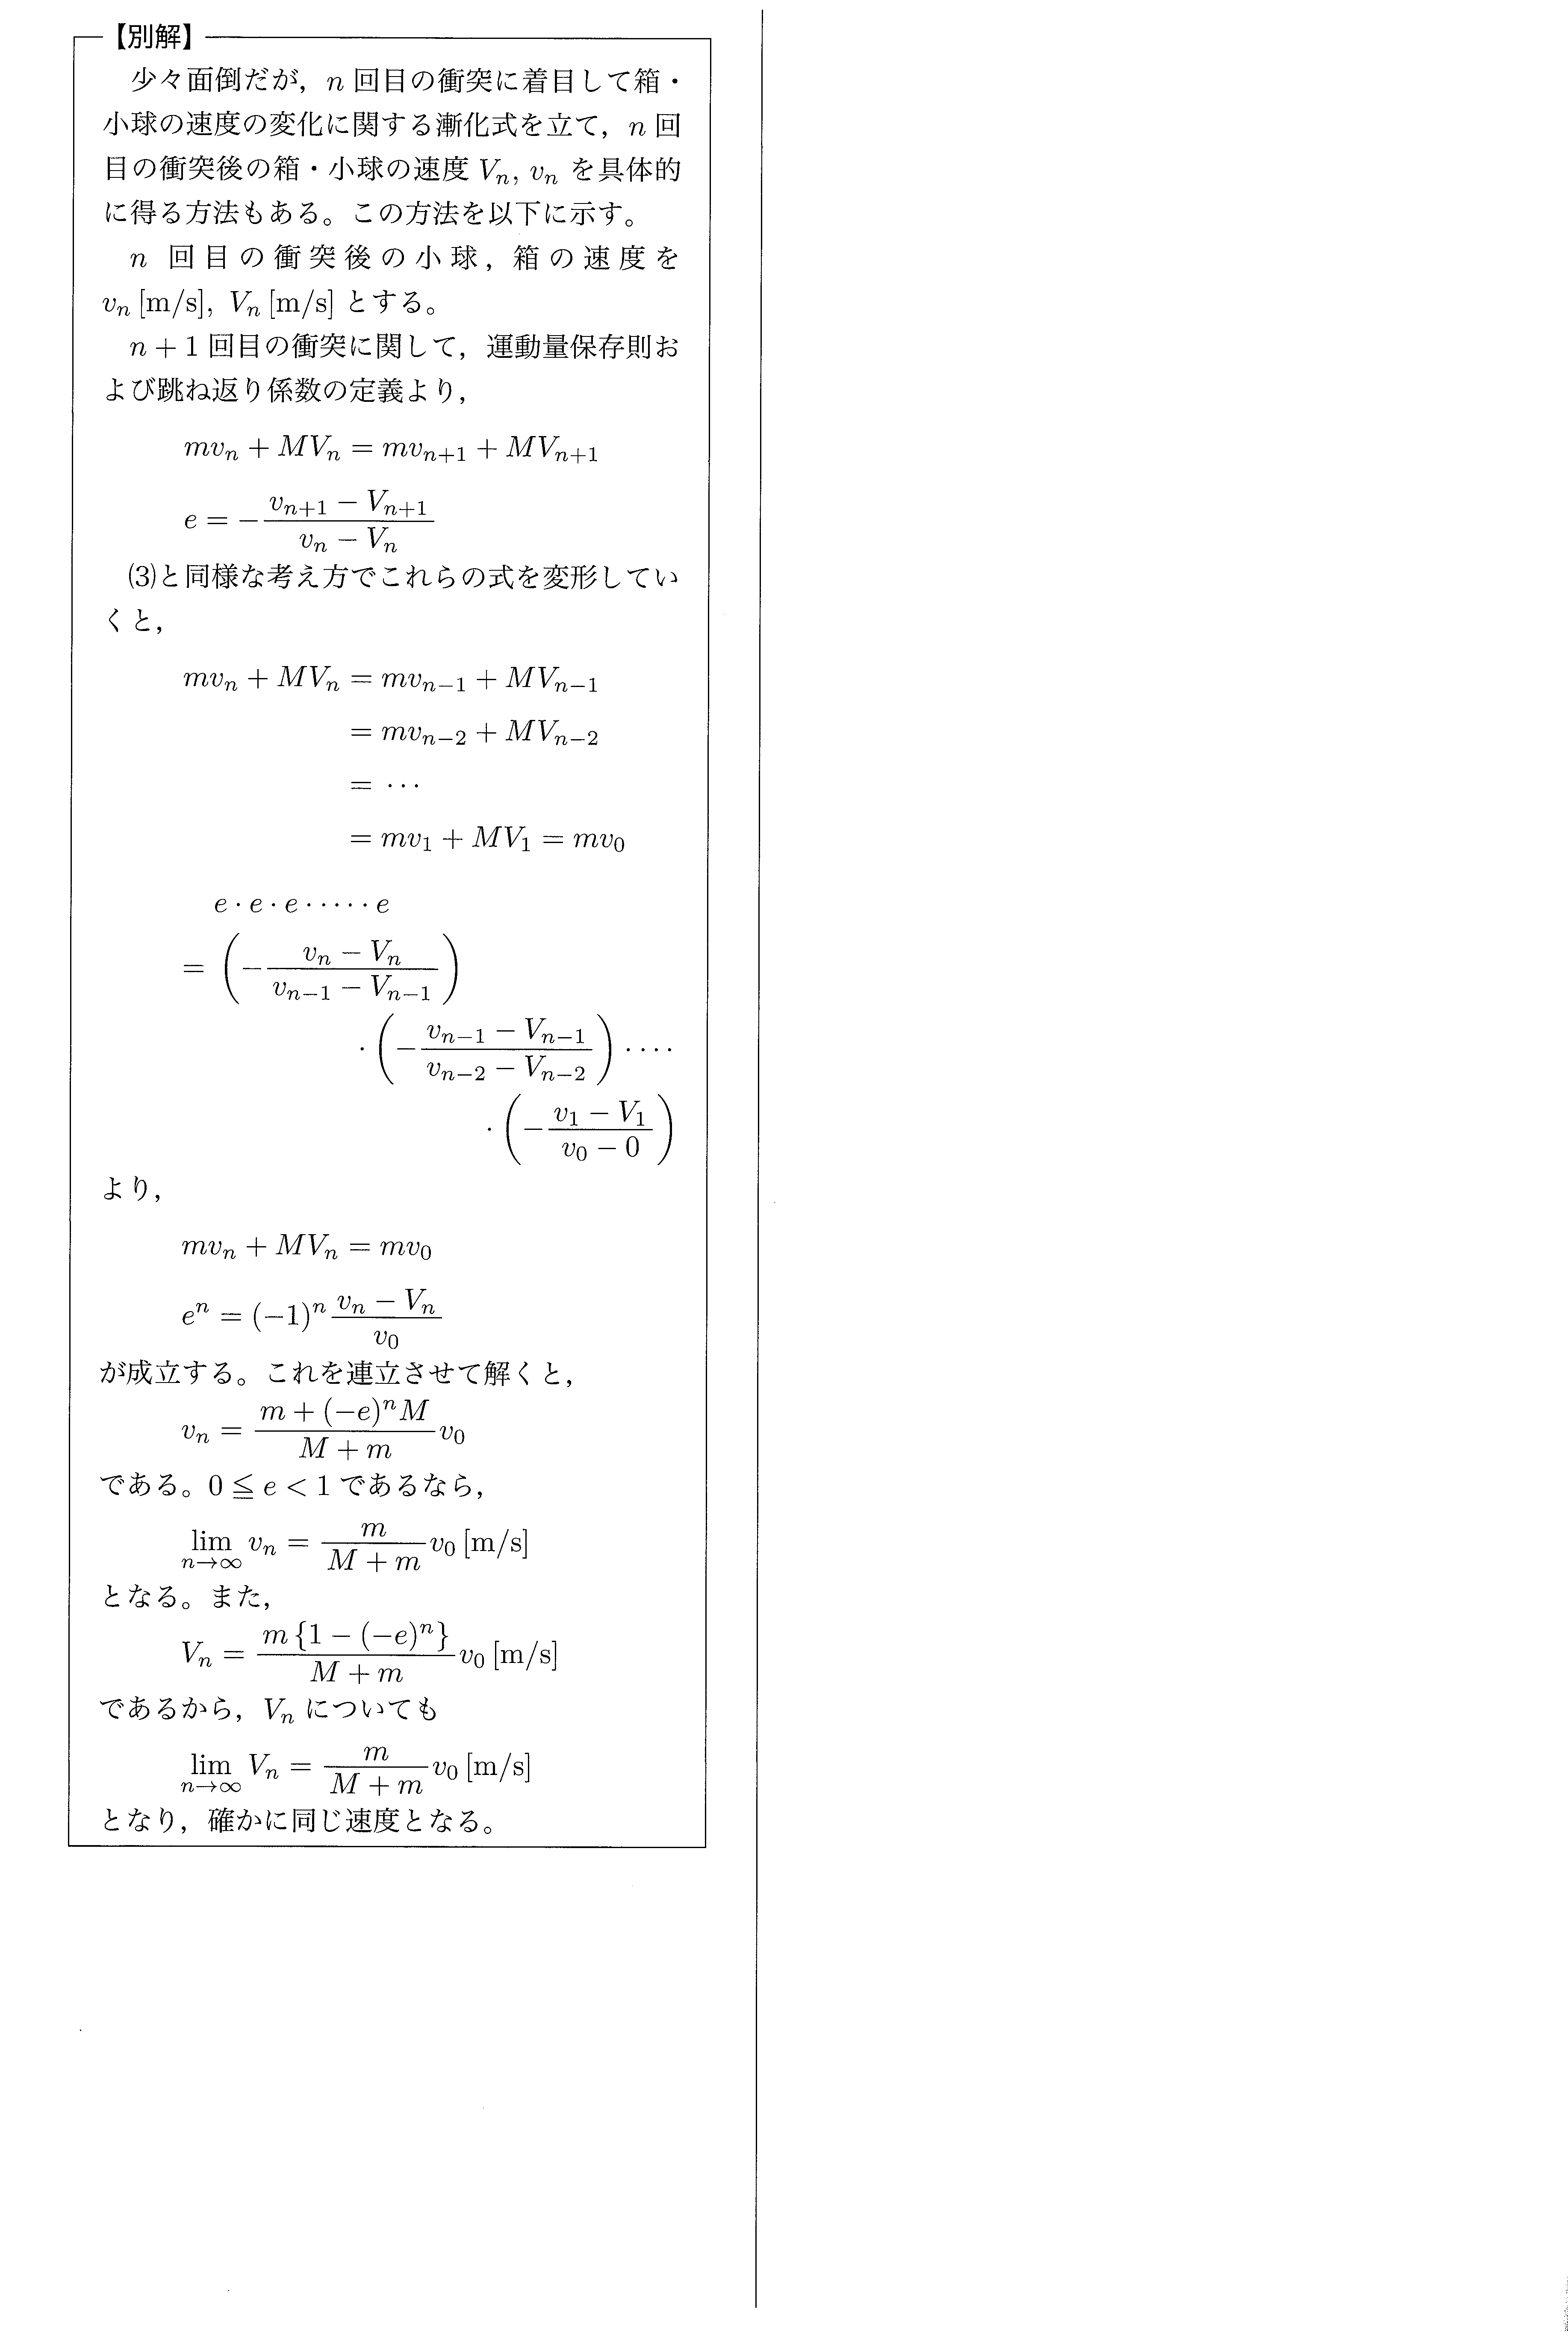
\includegraphics[width=170mm]{prob_p92_1.png}
\end{center}
\end{figure}

\newpage
　

\section{円運動}

\subsection{角速度と等速円運動}

\begin{wrapfigure}[10]{r}[5mm]{60mm}
  \centering
  \vspace{-5mm}
  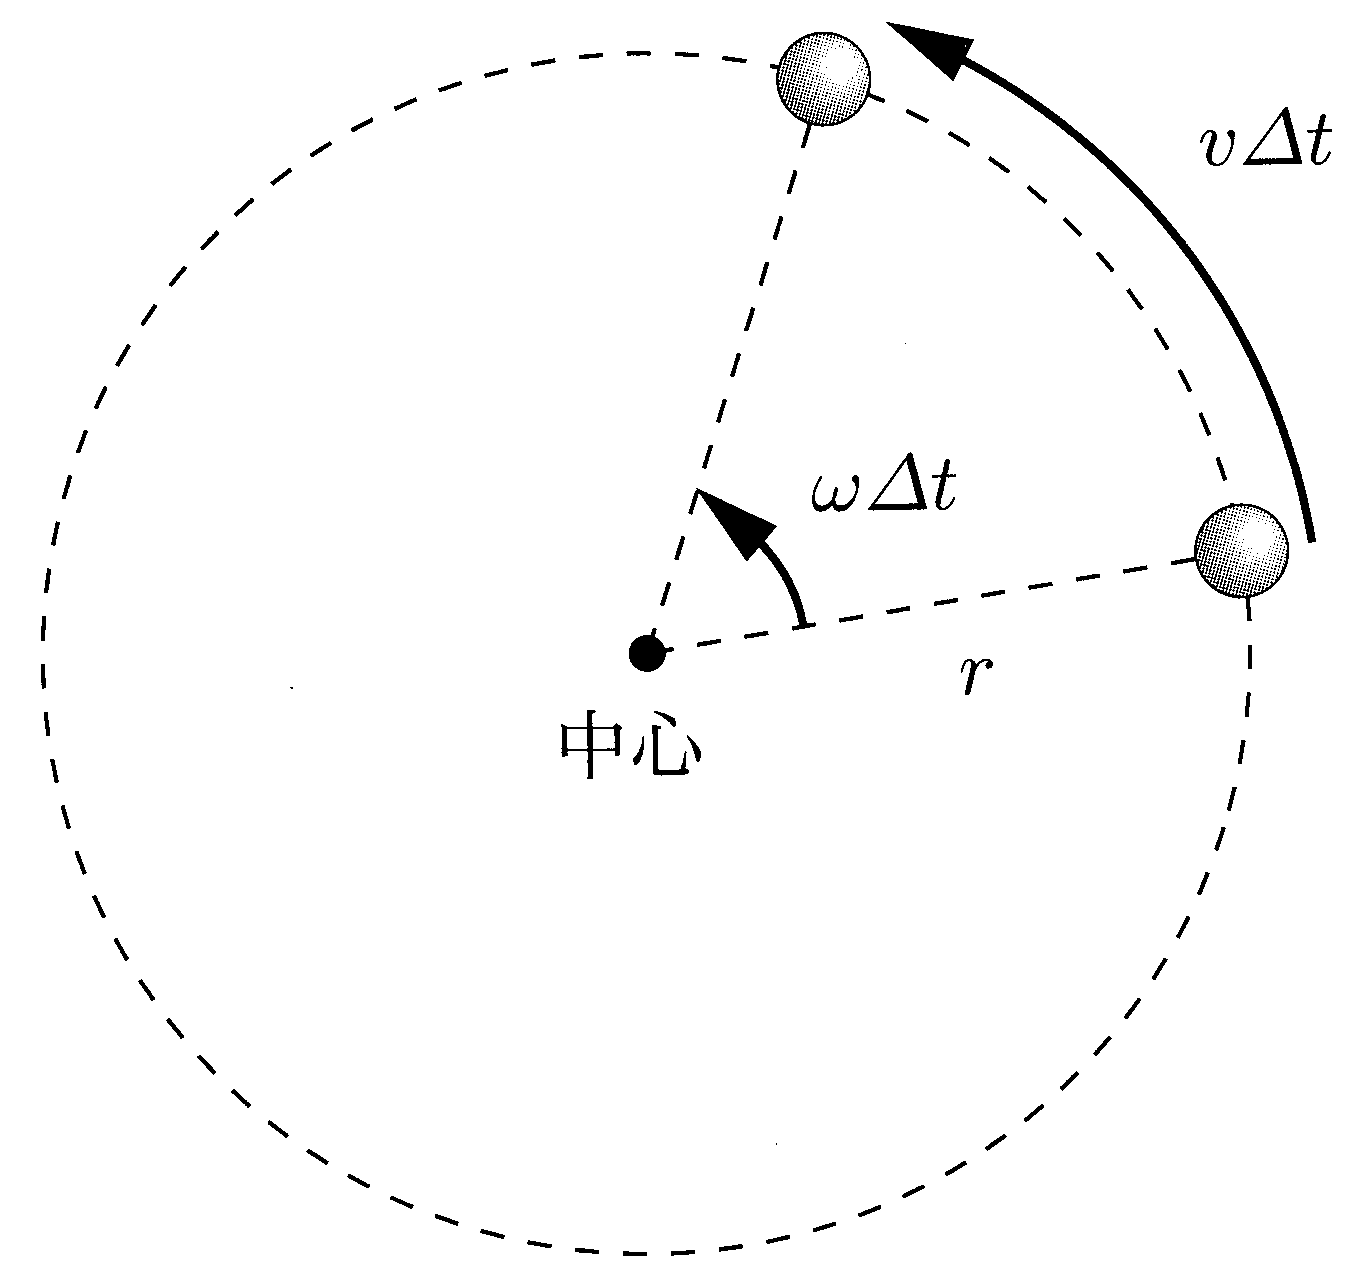
\includegraphics[keepaspectratio,width=50mm]
  {text_p36_fig1.png}
\end{wrapfigure}

右図のように，円周の上をなぞって物体が運動することを{\bf 円運動}という．

円運動する物体と円の中心を結ぶ線分{\bf （動径）}が単位時間（1秒間）に掃く中心角を{\bf 角速度} \mbox{\boldmath $\omega$} {\bf [rad/s]}という．
角速度が一定値であるとき物体の回転する速さは一定値となるので，このような円運動も{\bf 等速円運動}と呼ぶ．
角速度が$\omega$[rad/s]の等速円運動において，時間$\Delta t$[s]の間に物体が回転する角度$\theta$は，
\[ \theta =\omega \Delta t\]
で与えられる．
ここでは簡単のため，等速円運動に話を限定して取り扱うことにする．

物体が円を一周するのに要する時間を{\bf 周期}という．
角度$2\pi$だけ回ると円を一周することになるので，円運動の周期$T$[s]は
\[ T=\dfrac{2\pi}{\omega} \hspace{2mm}[{\rm s}]\]
で与えられる．
また，1秒間の回転数$f$（単位は[回/s]=[Hz]（ヘルツ）を用いる）は$f=\dfrac{1}{T}$となる．

半径$r$[m]の円周上を円運動する物体について考える．
物体の速度ベクトルは物体の経路の接線方向を向くから，{\bf 円運動する物体の速度ベクトルは必ず円の接線方向を向く．}
物体の速さ$v$[m/s]とすると，時間$\Delta t$[s]の間に物体は$v\Delta t$[m]だけ移動し，中心角は$\omega \Delta t$変化するから，
\[ v\Delta t =r・\omega \Delta t \hspace{2mm}\Leftrightarrow \hspace{2mm}\mbox{\boldmath $v=r\omega$} \hspace{2mm}{\rm [m/s]} \]
と速さは与えられる． 

\begin{wrapfigure}[14]{r}[5mm]{80mm}
  \centering
  \vspace{-5mm}
  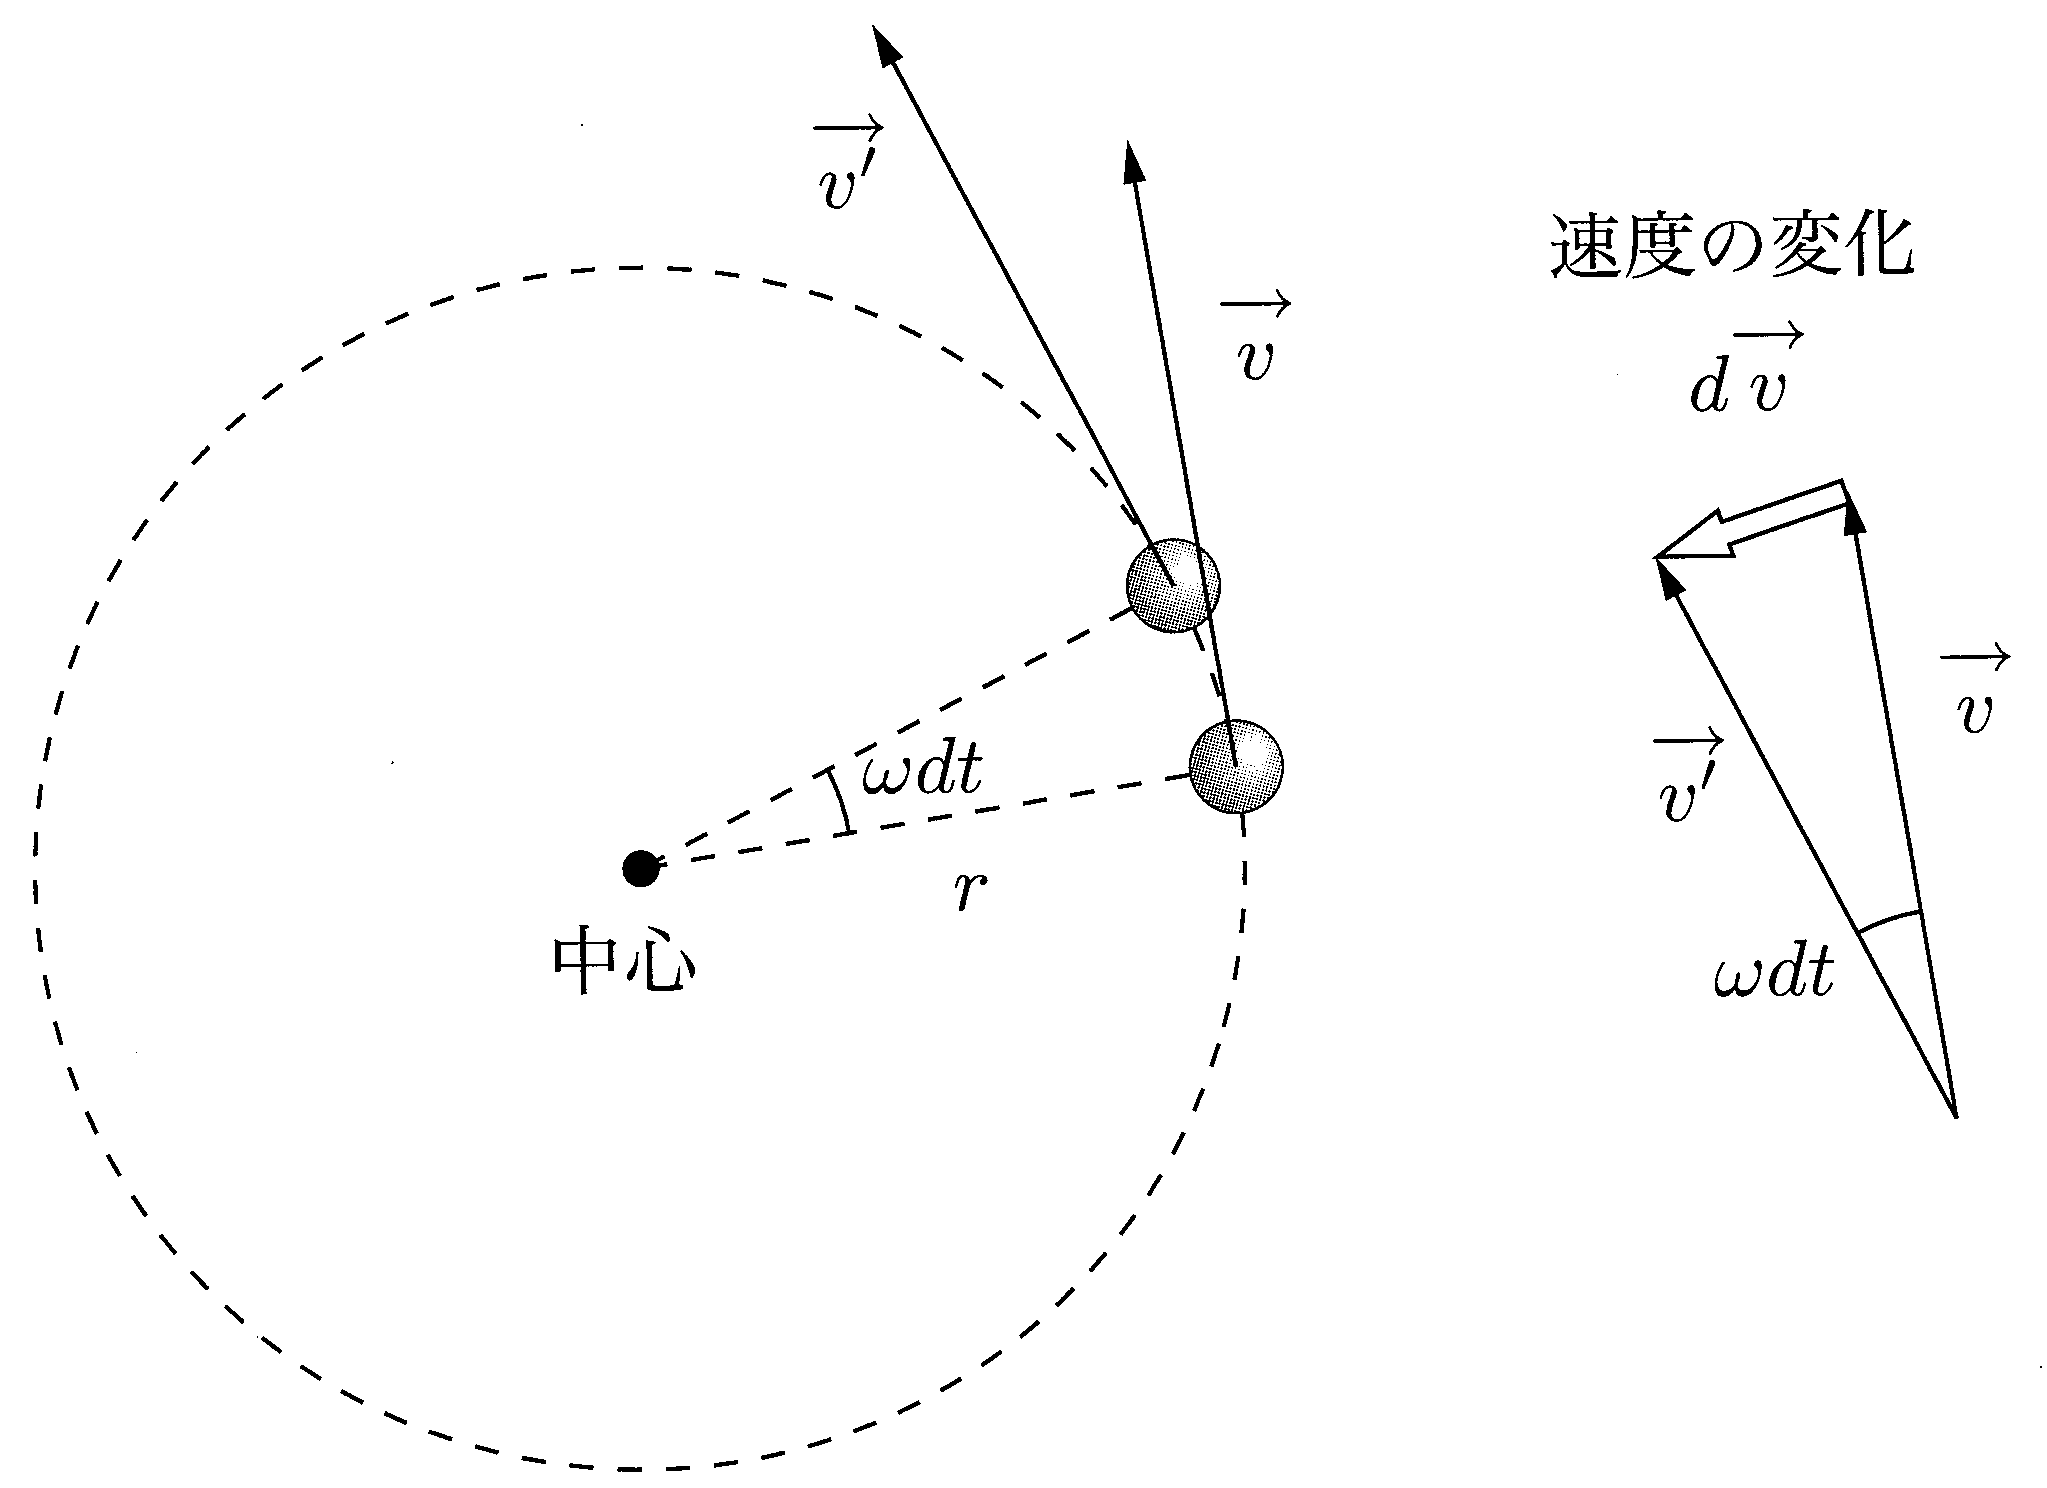
\includegraphics[keepaspectratio,width=75mm]
  {text_p36_fig2.png}
\end{wrapfigure}

物体が等速円運動を行うとき，速さは一定値であるが，速度ベクトルの向きは時々刻々と変化するから，物体は加速度を持っている．
微小時間$dt$[s]の間に速度ベクトルが$\overrightarrow{v \mathstrut}$[m/s]から$\overrightarrow{v' \mathstrut}$[m/s]に変化したとする．
変化した速度ベクトルを始点を揃えて書き出すと，この時間内での速度ベクトルは
\[ d\overrightarrow{v}=\overrightarrow{v' \mathstrut}-\overrightarrow{v \mathstrut}\]
であるが，図より$d\overrightarrow{v \mathstrut}$は円の中心方向を向いている．
よって，{\bf 加速度ベクトル}\mbox{\boldmath $\overrightarrow{a}=\dfrac{d\overrightarrow {v}}{dt} {\rm [m/s^2]}$}{\bf は円の中心方向を向く．}
その大きさ$a {\rm [m/s^2]}$は，図より
\[ a=\dfrac{v・\omega dt}{dt}=\mbox{\boldmath $v\omega$}=\mbox{\boldmath $r\omega^2$}=\mbox{\boldmath $\dfrac{v^2}{r} \hspace{2mm}{\rm [m/s^2]}$} \]
で与えられる．
この加速度ベクトルは常に速度ベクトルに直交するため，速度ベクトルの大きさは変えず，その向きのみを変える役割を果たす．

\begin{matome}{等速円運動}
 \hspace{5mm} 周期\hspace {8mm}$T=\dfrac{2\pi}{\omega}=\dfrac{2\pi r}{v}$\hspace{2mm}[s]\\
 \hspace{5mm} 速さ\hspace {8mm}$v=r\omega$\hspace{2mm}[m/s]　（速度は常に接線方向を向く）\\
 \hspace{5mm} 加速度\hspace {5mm}$a=r\omega^2=\dfrac{v^2}{r}\hspace{2mm}[{\rm m/s^2}]$　（加速度は常に中心方向を向き，速度ベクトルの向きを変える）
 \end{matome}

なお，物体の持つ加速度の大きさなどは円を座標軸に置き，物体の座標を時刻で微分することによっても得られる．

\begin{wrapfigure}[10]{r}[5mm]{60mm}
  \centering
  \vspace{-5mm}
  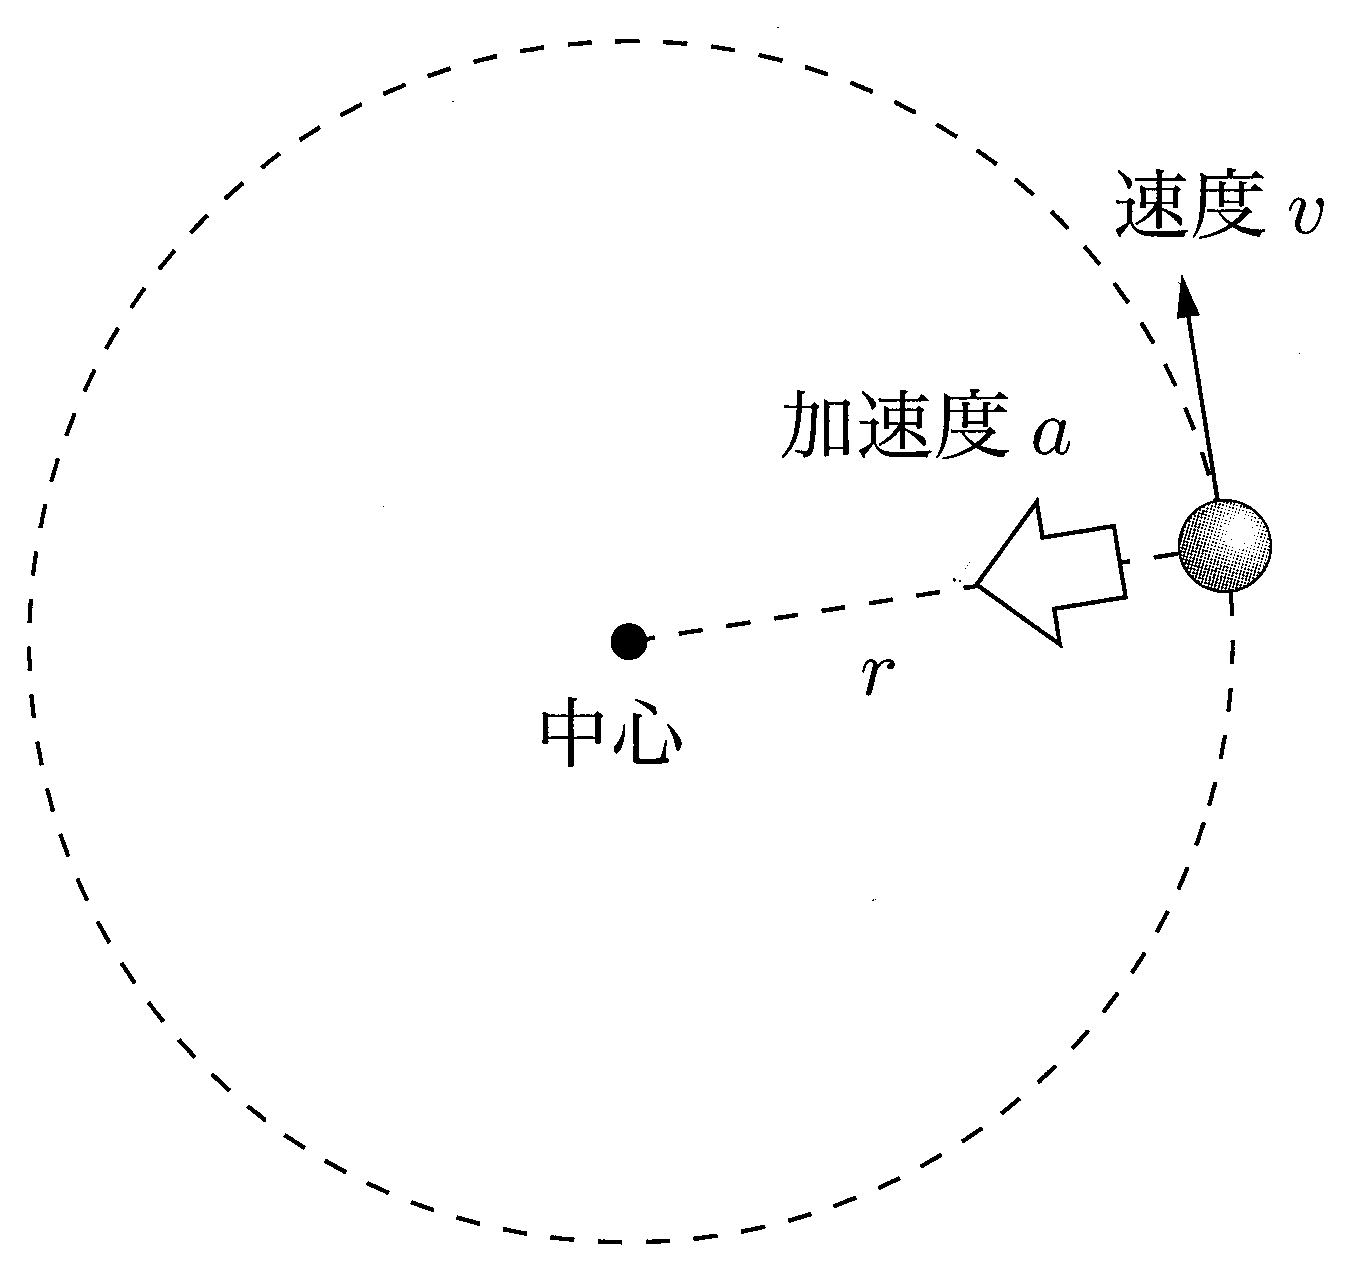
\includegraphics[keepaspectratio,width=50mm]
  {text_p37_fig1.png}
\end{wrapfigure}

円運動をする物体は加速度を持つが，このことから円運動をする物体には必ず力が作用していなければならない．
物体には様々な力が作用しているが，この力を接線方向と動径方向とに成分分解したときに，{\bf 動径方向に作用している力（の成分）のことを向心力という．}

等速円運動する物体は中心向きに大きさ$a=r\omega^2=\dfrac{v^2}{r}\hspace{1mm}[{\rm m/s^2}]$の加速度を持つ．
このことから，運動方程式を用いて動径方向に作用している力を逆算すると，
\[ma=mr\omega^2=m\dfrac{v^2}{r} \hspace{1mm}{\rm [N]} \]
となる．すなわち{\bf 等速円運動している物体に作用する向心力の合力は，必ず中心向きに大きさ}\mbox{\boldmath $mr\omega^2=m\dfrac{v^2}{r}$}\hspace{1mm}{\bf [N]となっている．}

向心力とは中心方向の加速度を生じさせる力の総称であり，{\bf 向心力という名称の力が存在するのではない}ことに注意せよ．

\begin{matome}{向心力}
 \hspace{5mm} 物体に作用する力の動径方向成分の合力は常に中心向きで大きさは$mr\omega^2=m\dfrac{v^2}{r}$\hspace{1mm}[N]
 \end{matome}
 
 
 \ 
 
%\begin{breakbox}
%\ex＜等速円運動＞\\
%
%なめらかな水平面上に自然長$l_0$[m]，弾性定数$k$[N/m]の軽いバネの一端を軸に固定し，もう一方に質量$m$[kg]の小球を取り付ける．
%この小球を軸のまわりに回転させたところ，バネは自然長から$x$[m]だけ伸びた状態を保って等速円運動した．
%これについて以下の問いに答えよ．
%\begin{wrapfigure}[7]{r}[5mm]{60mm}
%  \centering
%%  \vspace{-5mm}
%  \includegraphics[keepaspectratio,width=53mm]
%  {text_p37_fig2.png}
%\end{wrapfigure}
%\begin{description}
%\item[(1)] 向心方向の運動方程式を立式し，小球の速さ$v$[m/s]を求めよ．
%\item[(2)] 小球の角速度$\omega$[rad/s]を求めよ．
%\item[(3)] 等速円運動の周期$T$[s],\hspace{1mm}1[s]あたりの回転数$f$[Hz]を求めよ．
%\end{description}
%
%\end{breakbox}

%\newpage
 \subsection{非等速円運動}
 
 {\bf 非等速円運動においても動径方向については等速円運動のときと同様に扱うことができる．}
 すなわち，その瞬間における物体の接線方向の速さを$v$[m/s]とすると，物体の持つ加速度の円の中心方向成分は$\dfrac{v^2}{r}\hspace{1mm}{\rm [m/s^2]}$ になっているといえる．
 これと力学的エネルギー保存則を組み合わせることで非等速円運動を解くことができる．
 
 \begin{matome}{非等速円運動}
 \hspace{5mm} $\MARU{1}$\hspace{2mm}力学的エネルギー保存則から物体の速さを求める\\
 \hspace{5mm} $\MARU{2}$\hspace{2mm}動径方向についての運動方程式を立てる
 \end{matome}
 
 
 \ 
 
%\begin{breakbox}
%\ex＜非等速円運動＞\\
%\begin{wrapfigure}[7]{r}[5mm]{75mm}
%  \centering
%  \vspace{-10mm}
%  \includegraphics[keepaspectratio,width=65mm]
%  {text_p38_fig1.png}
%\end{wrapfigure}
%\hspace{5mm}内面がなめらかな半径$r$[m]の半円筒をなめらかな水平面に接続して図のように置く．
%水平面上から質量$m$[kg]の小球を速さ$v_0$[m/s]で円筒の内面へ向けてすべらせたところ，小球は円筒面に沿って登っていき，最高点Q点を通過した．
%これについて以下の問いに答えよ．
%ただし，重力加速度の大きさを$g {\rm [m/s^2]}$とし，運動は図の面内でのみ起こるものとせよ．
%\begin{description}
%\item[(1)] 図のP点を通過するときの物体の速さ$v_1$[m/s]を求めよ．
%\item[(2)] 図のP点において物体が円筒面から受ける垂直抗力の大きさ$N_1$[N]を求めよ．
%\item[(3)] 図のQ点を通過するときの物体の速さ$v_2$[m/s]を求めよ．
%\item[(4)] 図のQ点において物体が円筒面から受ける垂直抗力の大きさ$N_2$[N]を$v_2$を用いて表せ．
%\item[(5)] 図のQ点において物体が円筒面から離れないために必要な$v_2$の条件式を求めよ．
%\item[(6)] 図のQ点を通過させるために必要な初速についての条件を求めよ．
%\end{description}
%
%\end{breakbox}


 \newpage

\begin{figure}[h]
\begin{center}
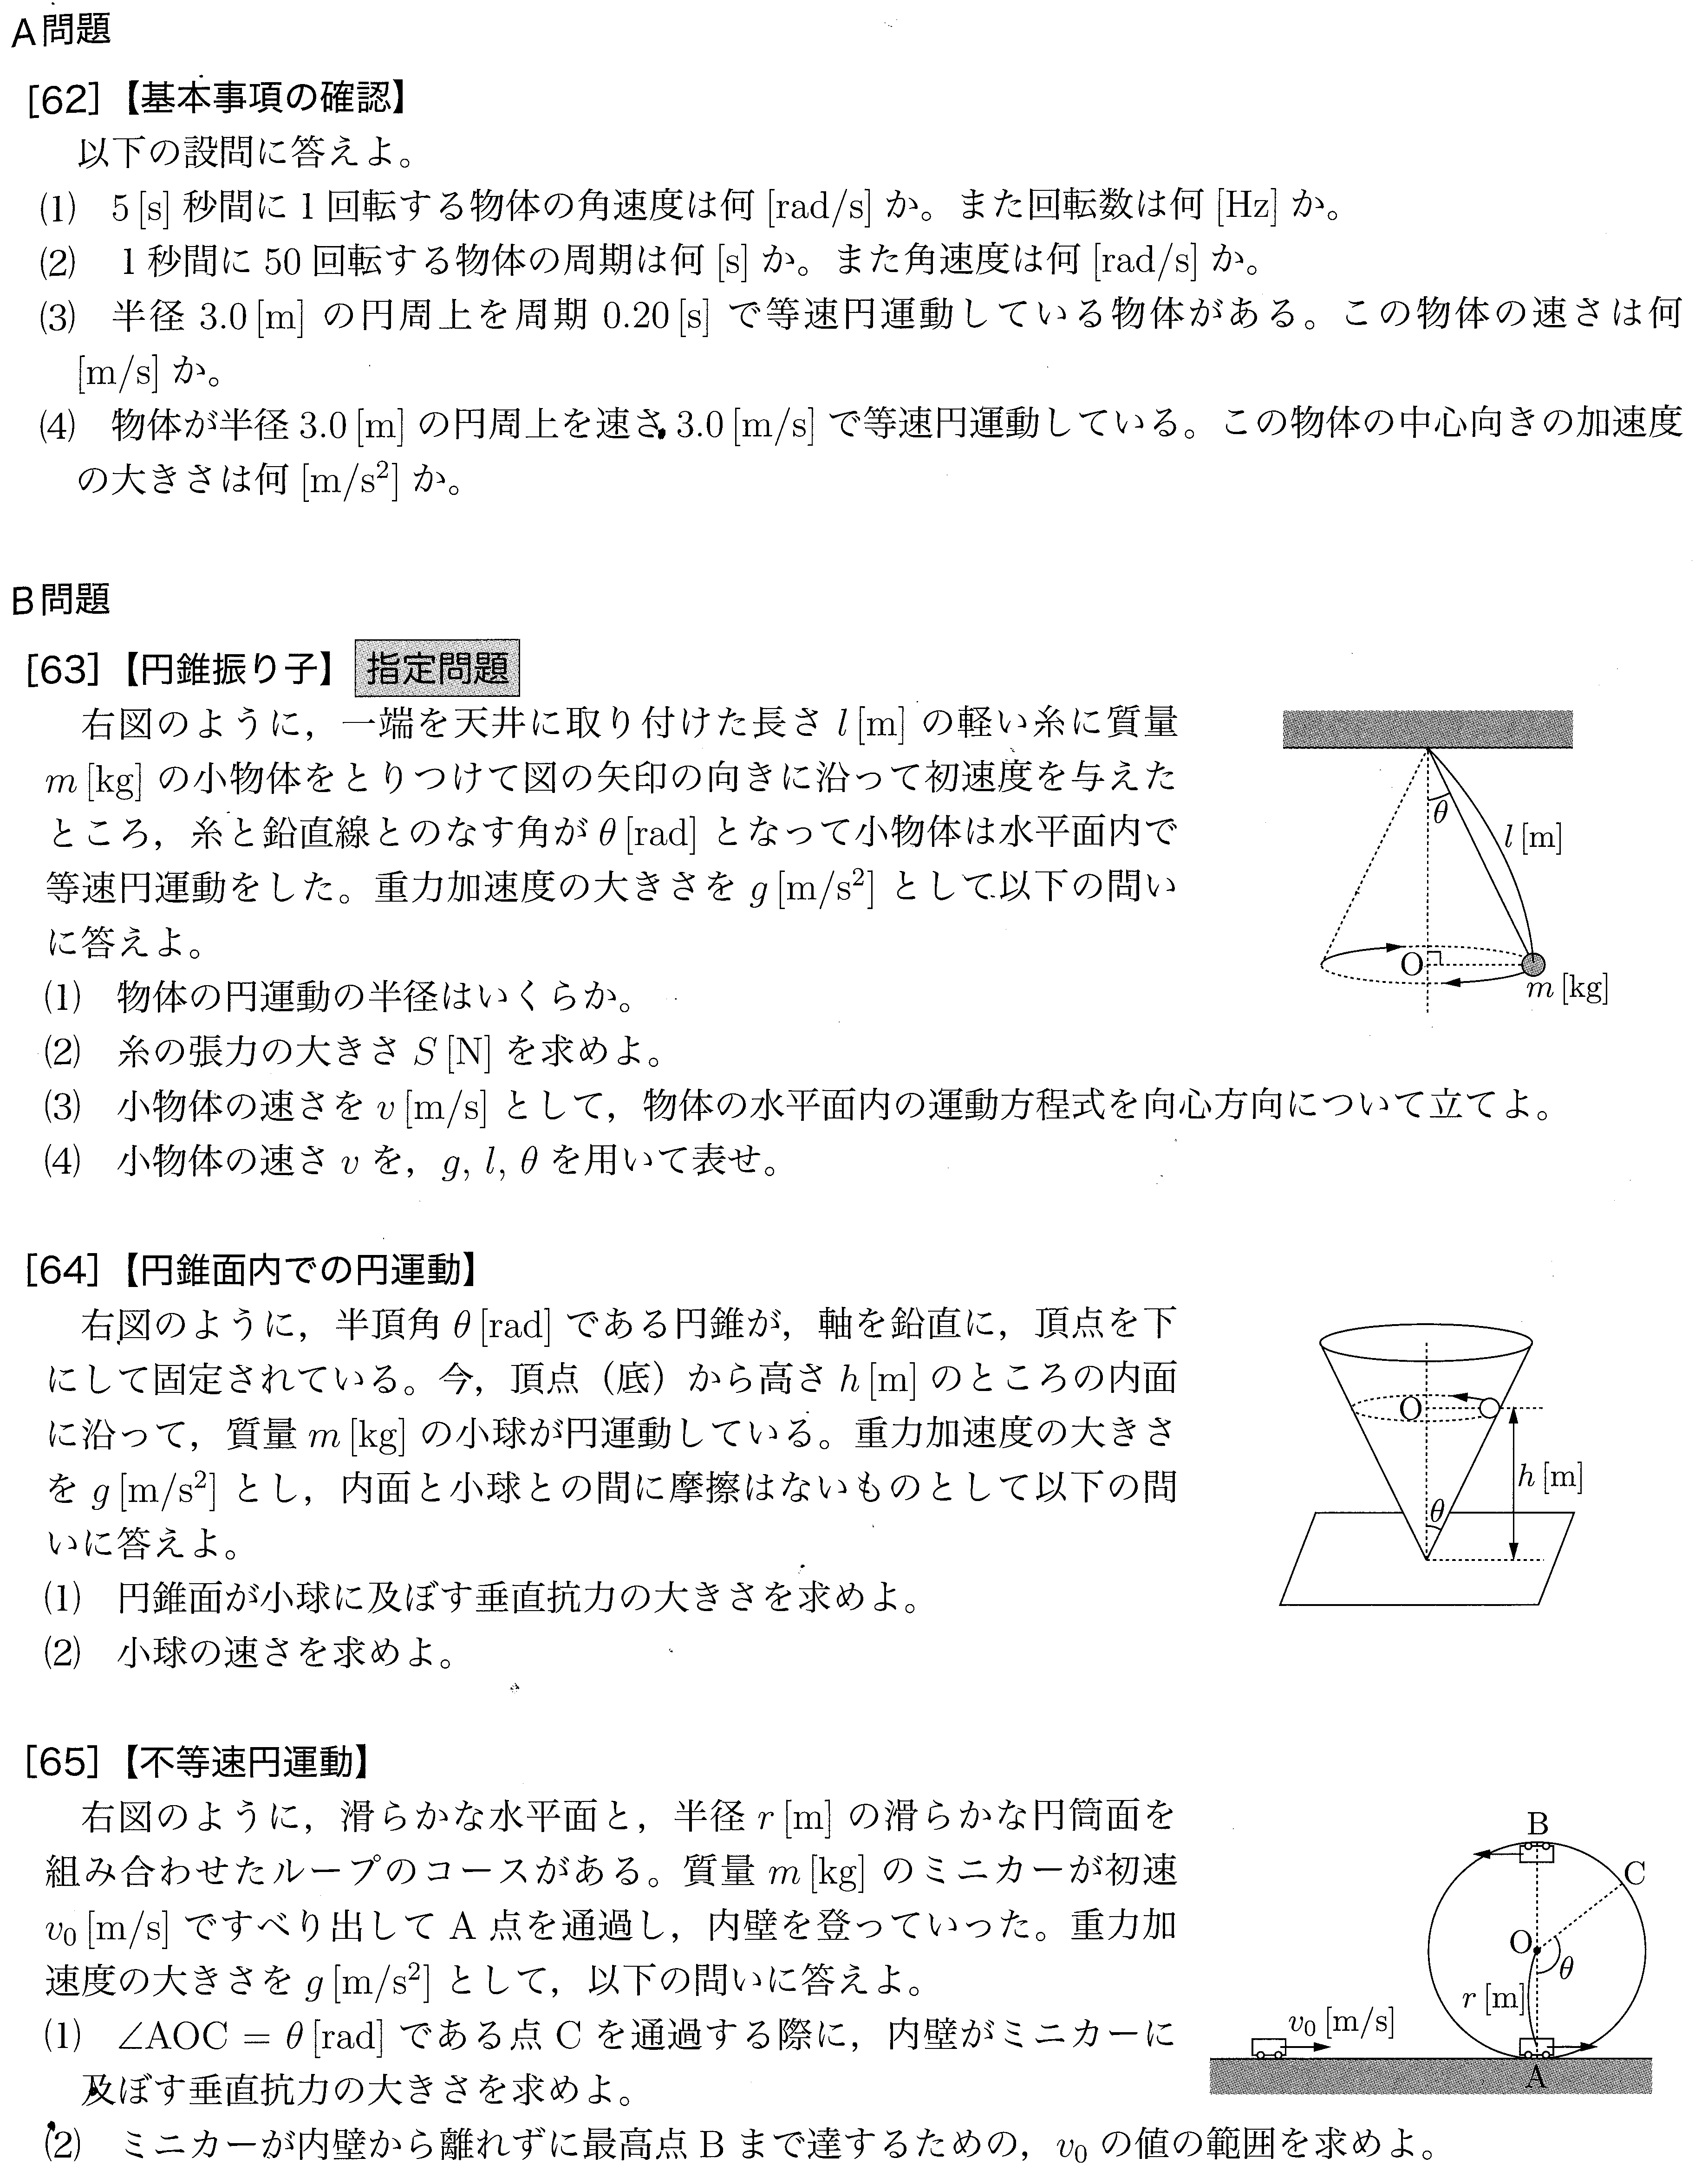
\includegraphics[width=170mm]{prob_p21.png}
\end{center}
\end{figure}

\newpage

\begin{figure}[h]
\begin{center}
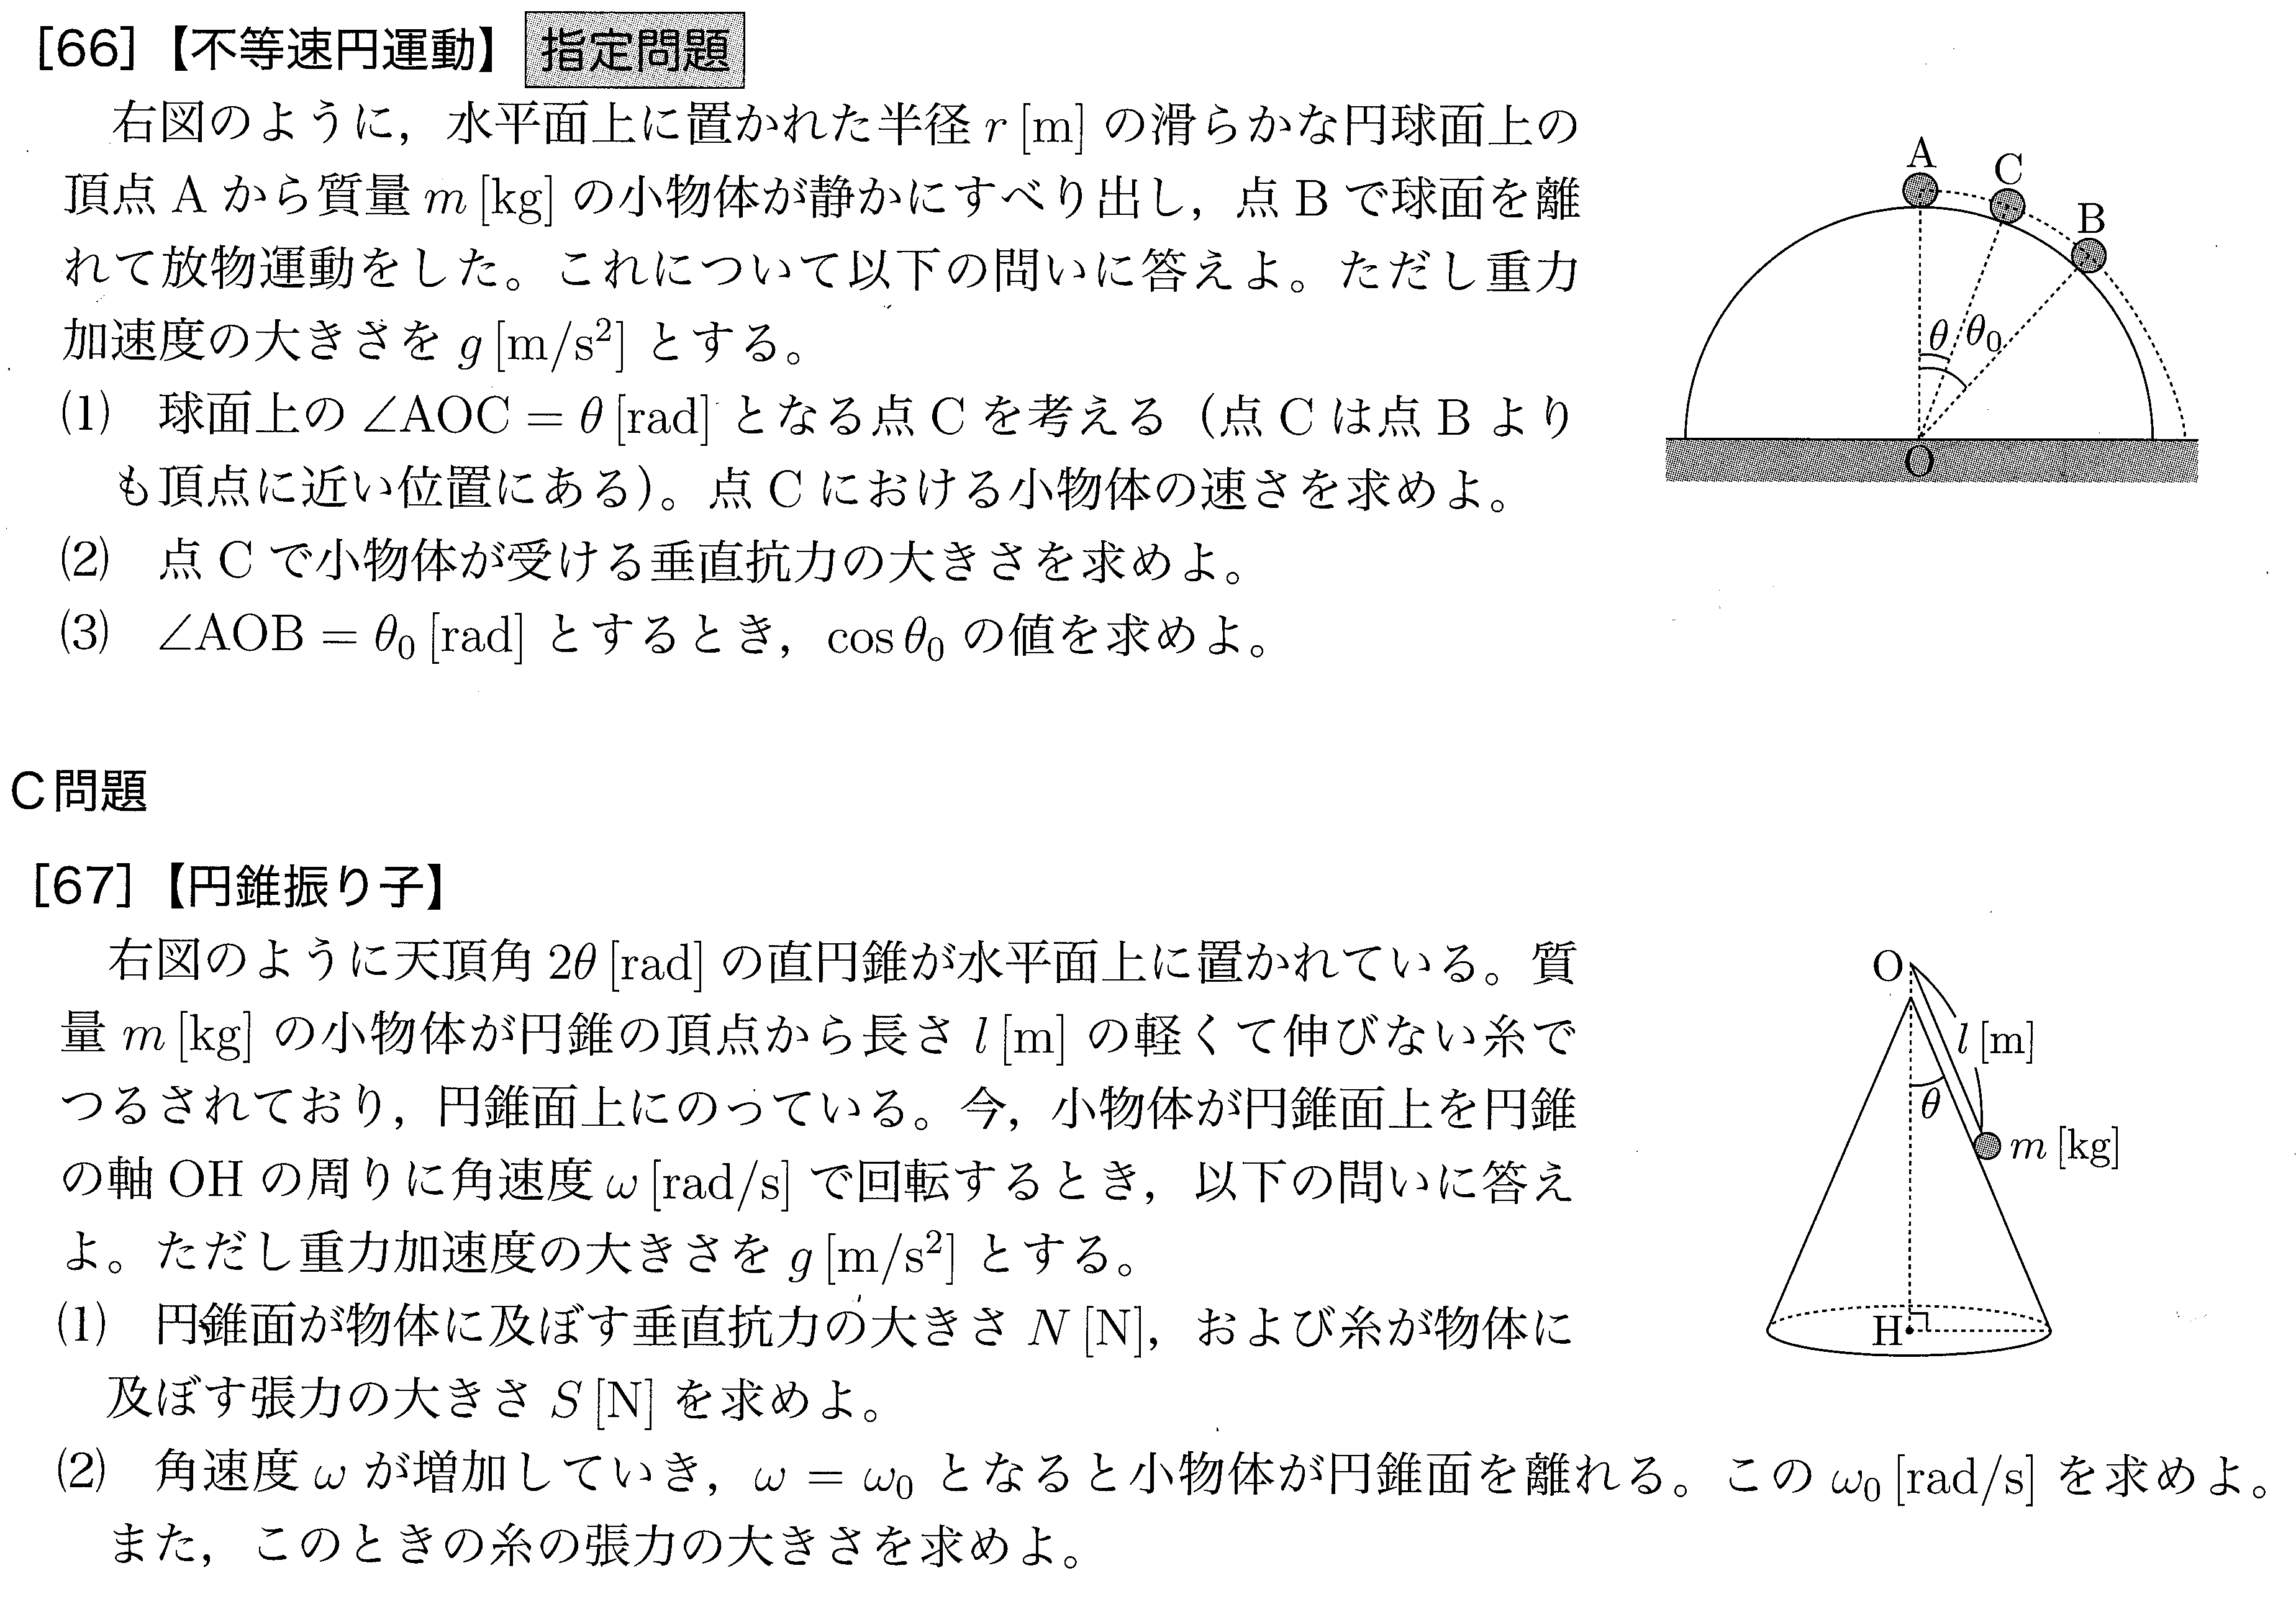
\includegraphics[width=170mm]{prob_p22.png}
\vspace{10cm}
\end{center}
\end{figure}



\newpage

\begin{figure}[h]
\begin{center}
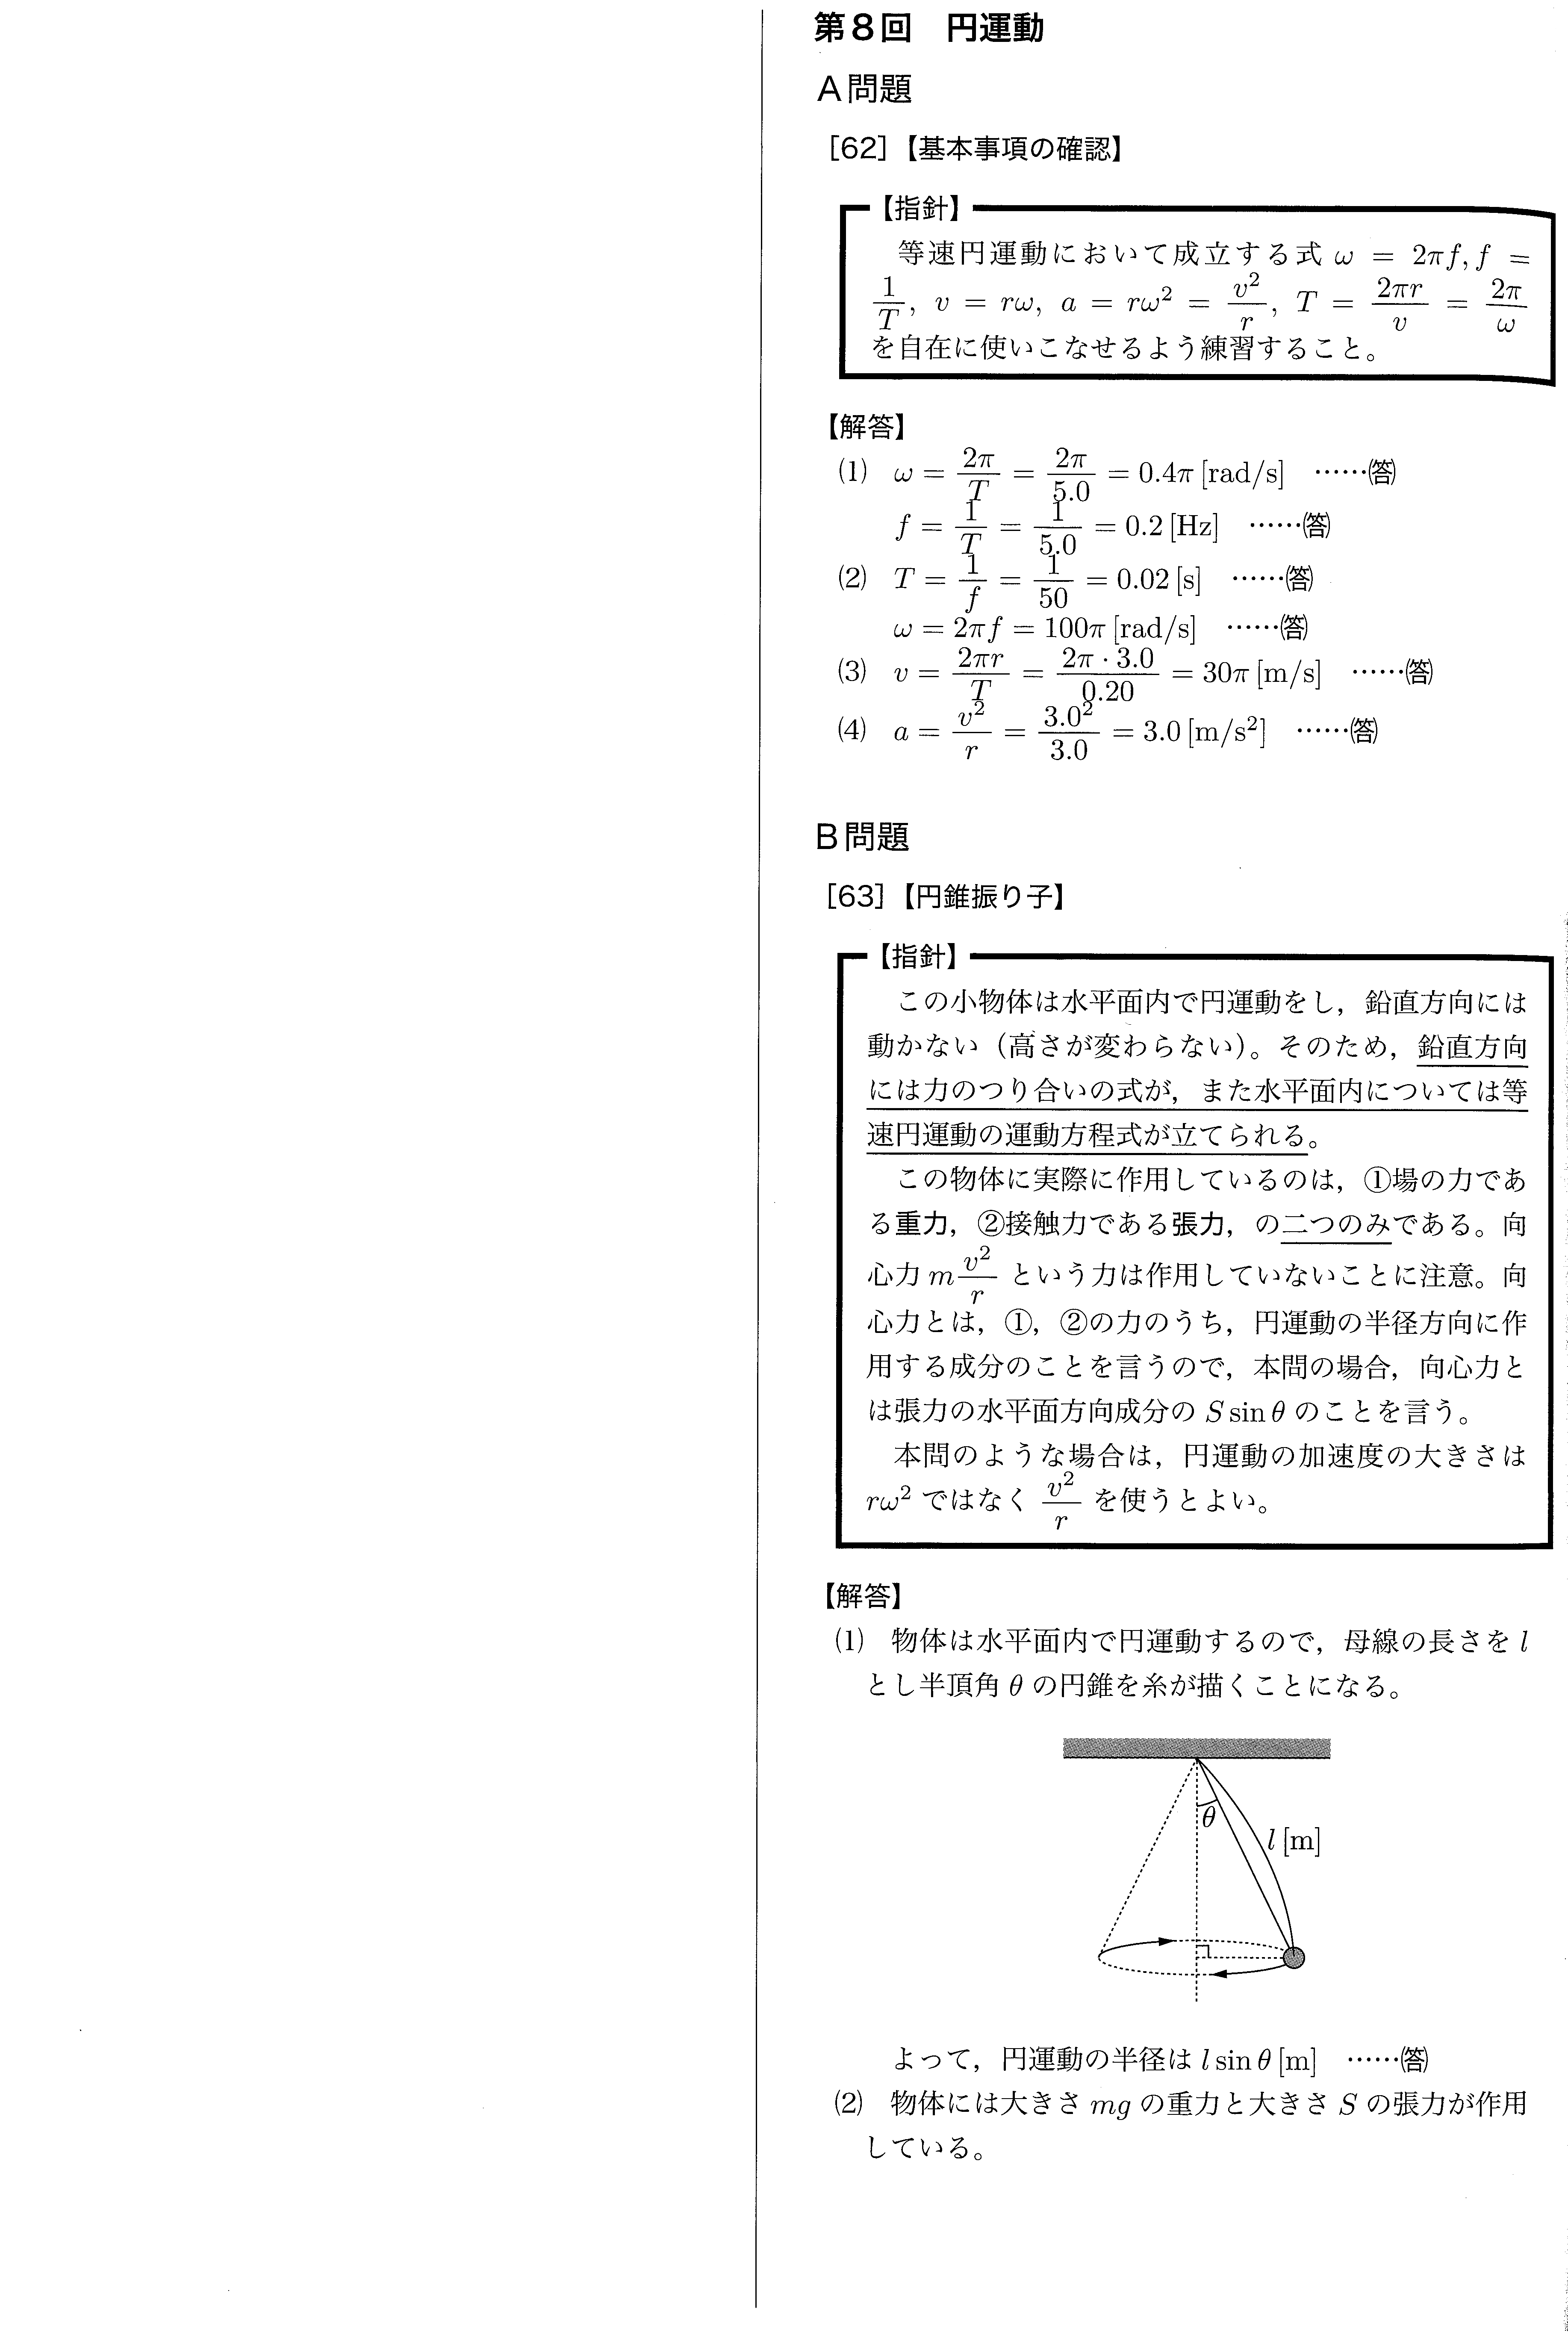
\includegraphics[width=170mm]{prob_p92_2.png}
\end{center}
\end{figure}

\newpage

\begin{figure}[h]
\begin{center}
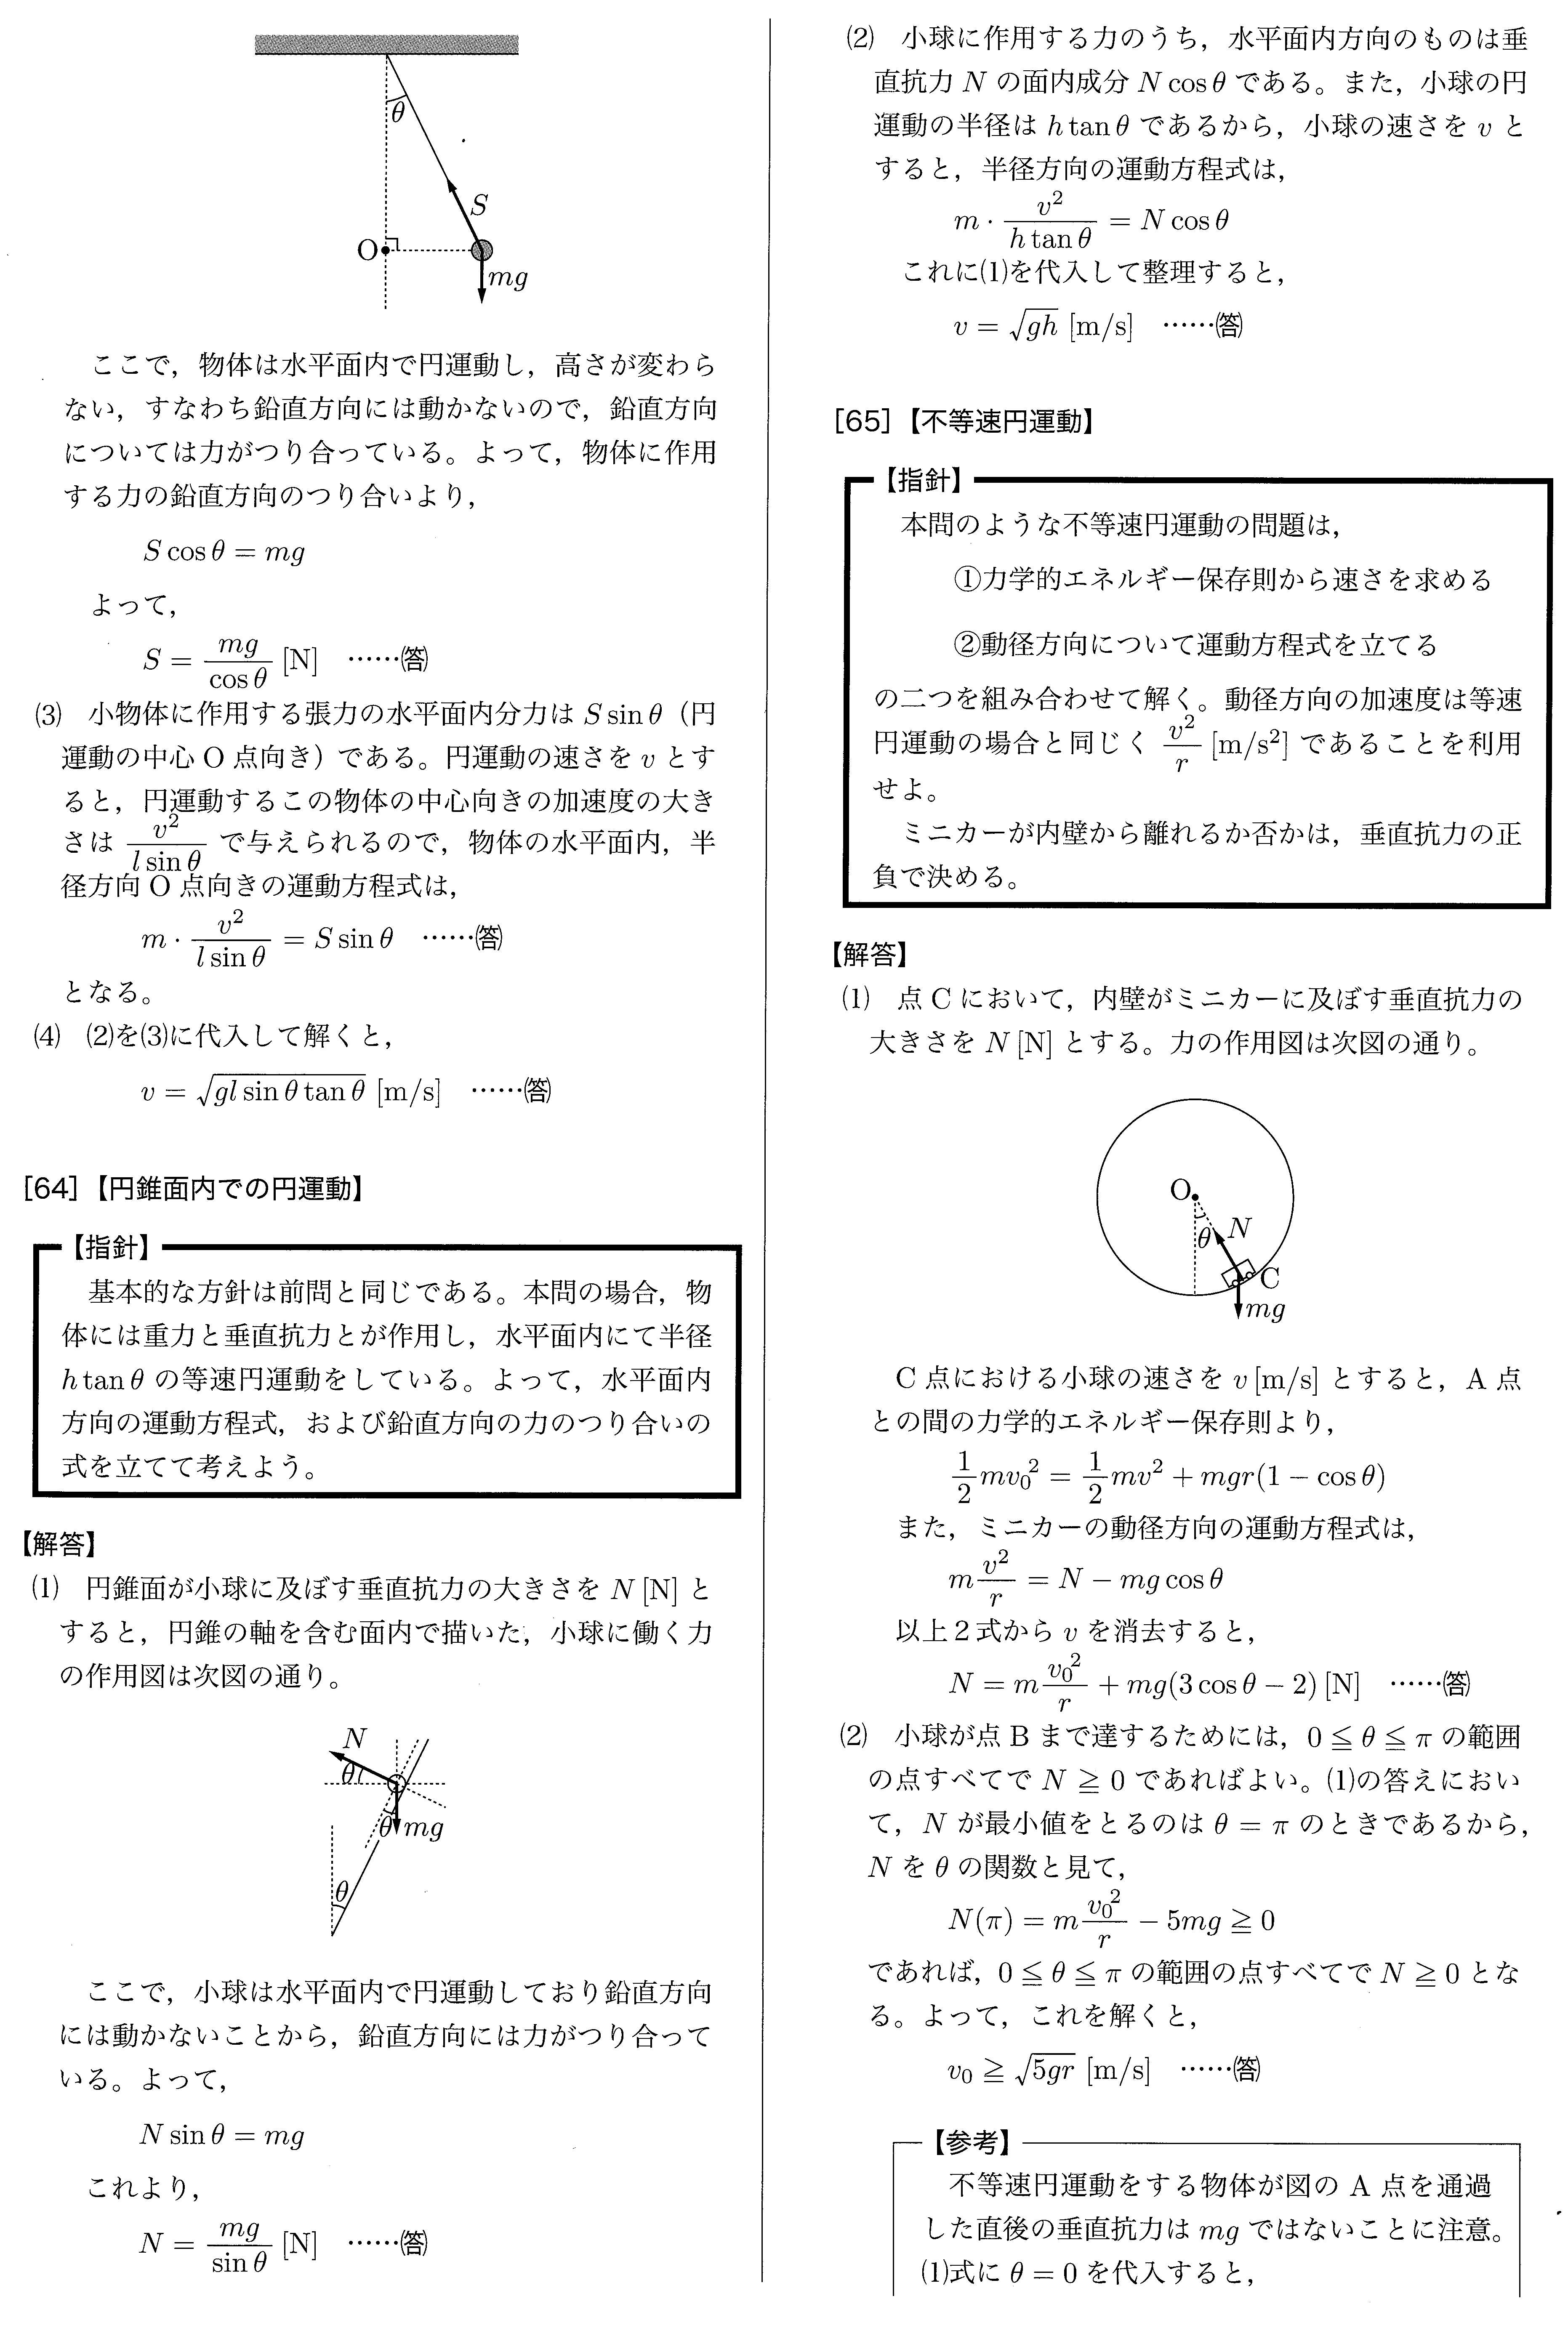
\includegraphics[width=170mm]{prob_p93.png}
\end{center}
\end{figure}

\newpage

\begin{figure}[h]
\begin{center}
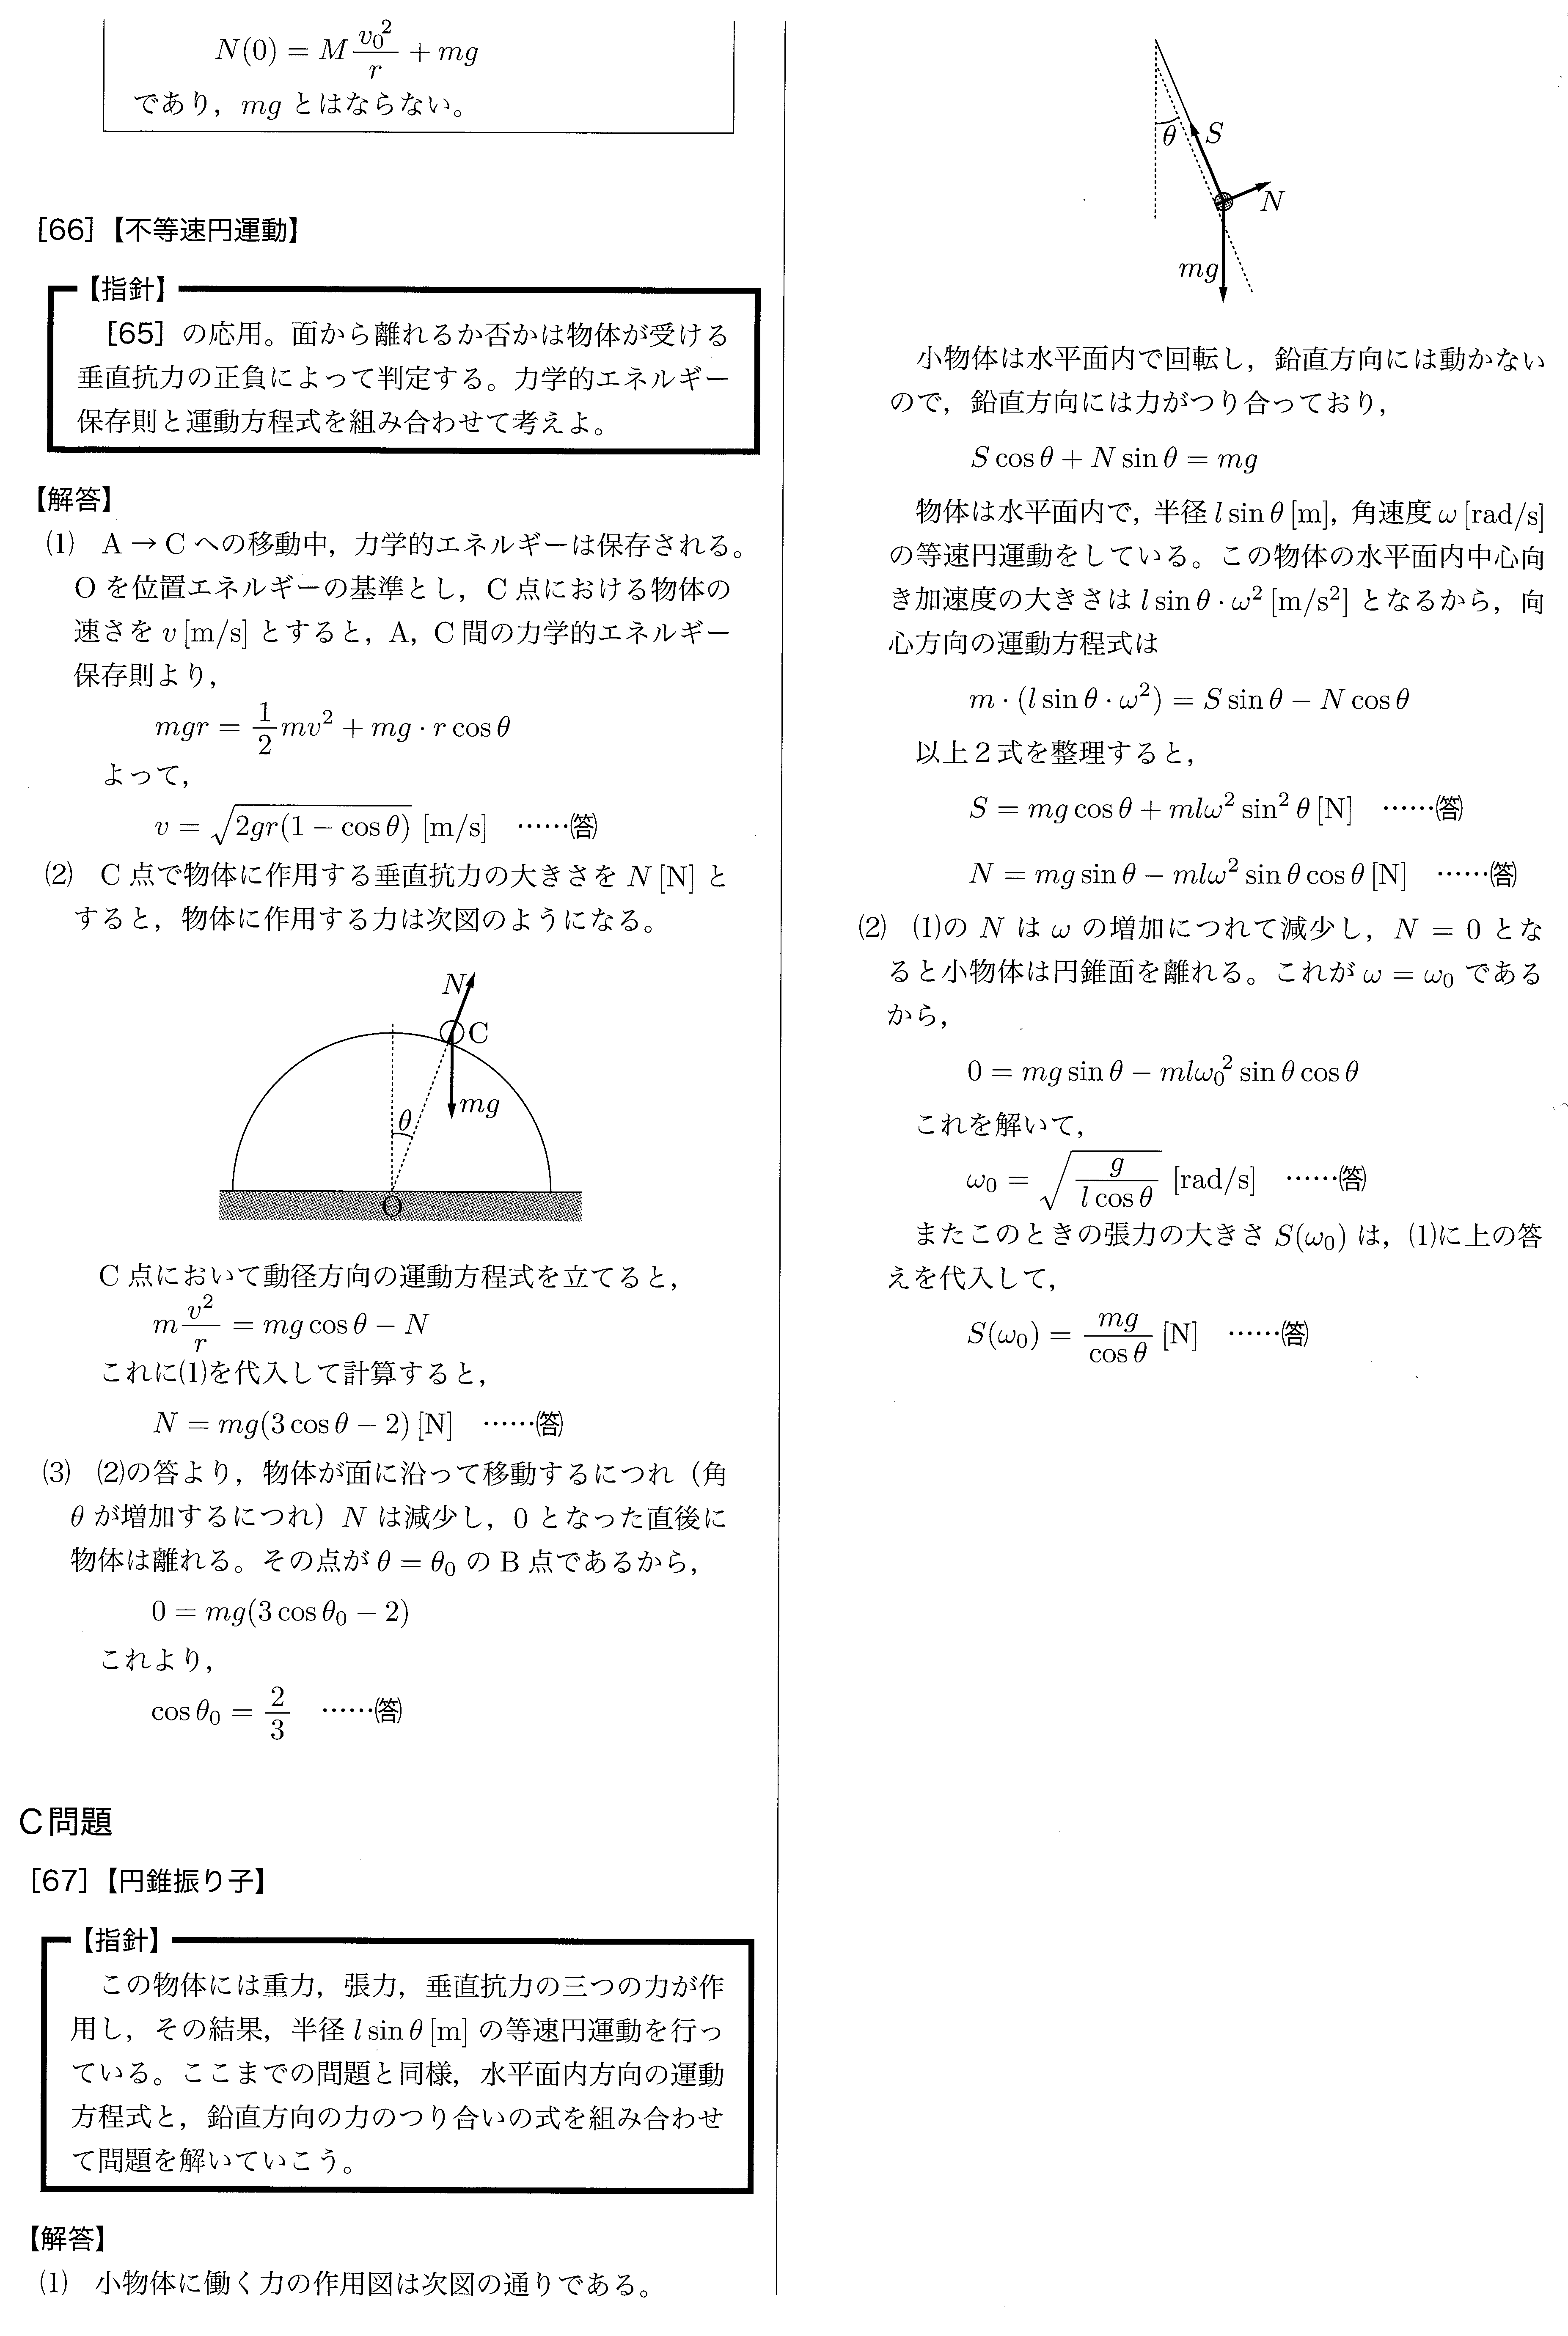
\includegraphics[width=170mm]{prob_p94.png}
\end{center}
\end{figure}

 \ 
 
\newpage
\section{単振動}

\subsection{単振動}

\begin{wrapfigure}[18]{r}[5mm]{60mm}
  \centering
  \vspace{-5mm}
  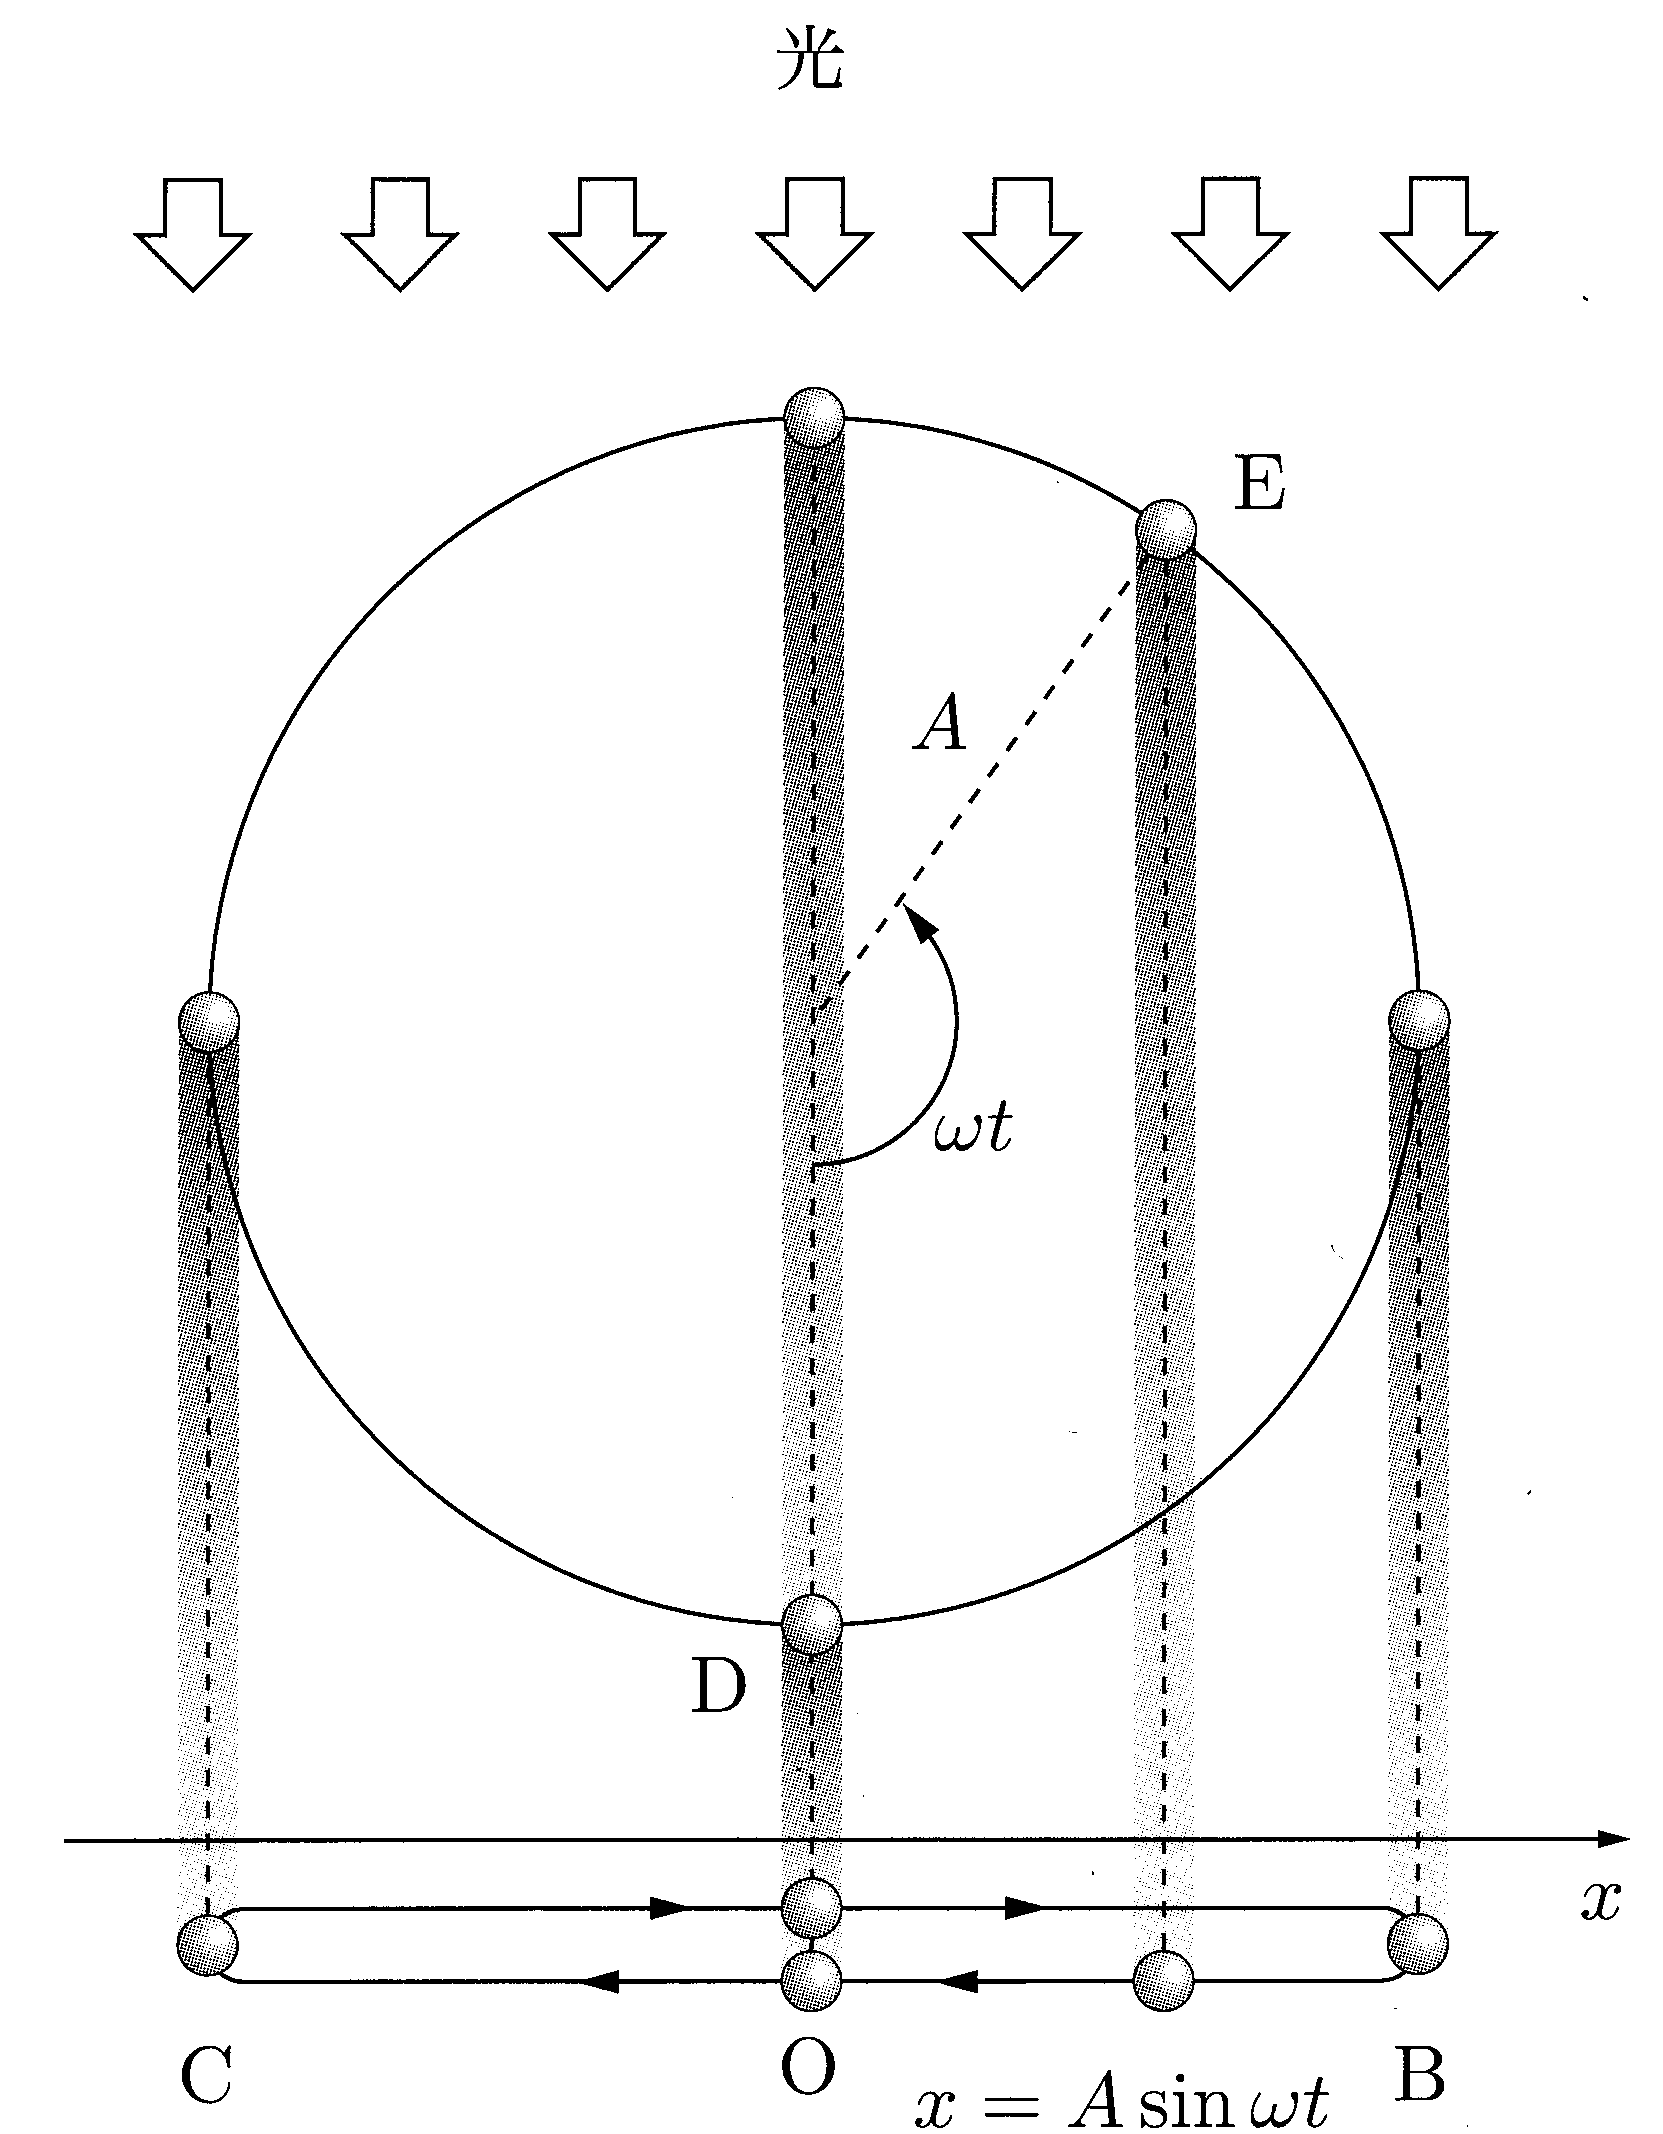
\includegraphics[keepaspectratio,width=60mm]
  {text_p39_fig1.png}
\end{wrapfigure}

質点が図のように半径$A$[m]，角速度$\omega$[rad/s]の等速円運動を行っているとき，図の方向から光を当ててその影の運動を観察すると，影は図の$x$軸上の$O$点を中心として，$B$点と$C$点の間を往復運動する．

簡単のため，質点が図の$D$点を通過した時刻を$t=0$[s]として円運動をパラメータ表示すると，
\[(x,y)=(A\sin \omega t,A\cos \omega t) \]
であり，時刻$t$[s]におけるこの質点の投影点は
\[x=A\sin \omega t\]
となる．
今は質点が$D$点を通過した時刻を$t=0$[s]としたが，より一般には時刻$t=0$[s]における位置を考慮して，
\[ x=A\sin (\omega t+\varphi_0)\]
と書ける．
物体の位置がこのような形の式で書ける運動を{\bf 単振動}という．
単振動の中心からの振れ幅$A$[m]を単振動の{\bf 振幅}，$\omega$[rad/s]をその単振動の{\bf 角振動数}，時刻$t=0$[s]に物体がいた位置を表す$\varphi_0$を{\bf 初期位相}，三角関数の中身の部分$\omega t+\varphi_0$を{\bf 位相}という．

物体が単振動を行う典型例はバネに取り付けた物体の振動現象である．

 
 \ 
 
%\begin{breakbox}
%\ex＜単振動＞\\
%\begin{wrapfigure}[7]{r}[5mm]{60mm}
%  \centering
%%  \vspace{-5mm}
%  \includegraphics[keepaspectratio,width=53mm]
%  {text_p39_fig2.png}
%\end{wrapfigure}
%\hspace{5mm}物体が$x$軸上において単振動を行っている．
%時刻$t$[s]における物体の位置が
%\[ x=A\sin \omega t\]
%で与えられるとき，以下の問いに答えよ．
%ただし，$A$[m]および$\omega$[rad/s]は定数である．
%\begin{description}
%\item[(1)] この物体の時刻$t$[s]における速度および加速度を求めよ．
%\item[(2)] 物体の速さおよび加速度の大きさが最も大きくなる位置およびその値を求めよ．
%\item[(3)] 物体の速さが0[m/s]となる位置，および加速度の大きさが0${\rm [m/s^2]}$となる位置を求めよ．
%\item[(4)] この単振動の周期$T$[s]を求めよ．
%\item[(5)] 物体の加速度をその瞬間における物体の位置$x$[m]を用いて表せ．
%\item[(6)] 弾性定数$k$[N/m]のバネの先に図のように質量$m$[kg]の物体を取り付け，これをなめらかな床面の上で運動させる．この物体の運動方程式を書き，(5)と同じ形をしていることを示せ．
%\item[(7)] (5)と比較することで，(6)の単振動の角振動数$\omega'$[rad/s]および周期$T'$[s]を$m,k$を用いて表せ．
%\end{description}
%
%\end{breakbox}

 \ 
 
バネに取り付けた物体のように，運動方程式が
\[ma=-kx\hspace{3mm}（ただしkは正の定数）\]
なる関係にまとめられるとき，その物体は単振動することが知られている．

\begin{matome}{単振動と運動方程式}
 \hspace{5mm} 『運動方程式が$ma=-kx\hspace{5mm}(k>0)で表せる$』\\
 \hspace{12mm} $\Leftrightarrow $\hspace {1mm} 『$x=A\sin (\omega t+\varphi_0)$で表される単振動を行う』\\
 \hspace{5mm} 振動中心$x=0$\hspace {5mm}角振動数$\omega=\sqrt{\dfrac{k}{m}} $\hspace{5mm}周期$T=\dfrac{2\pi}{\omega}$
 \end{matome}
 
% 【端点ー振動中心ー端点】
% \begin{figure}[h]
%\begin{center}
%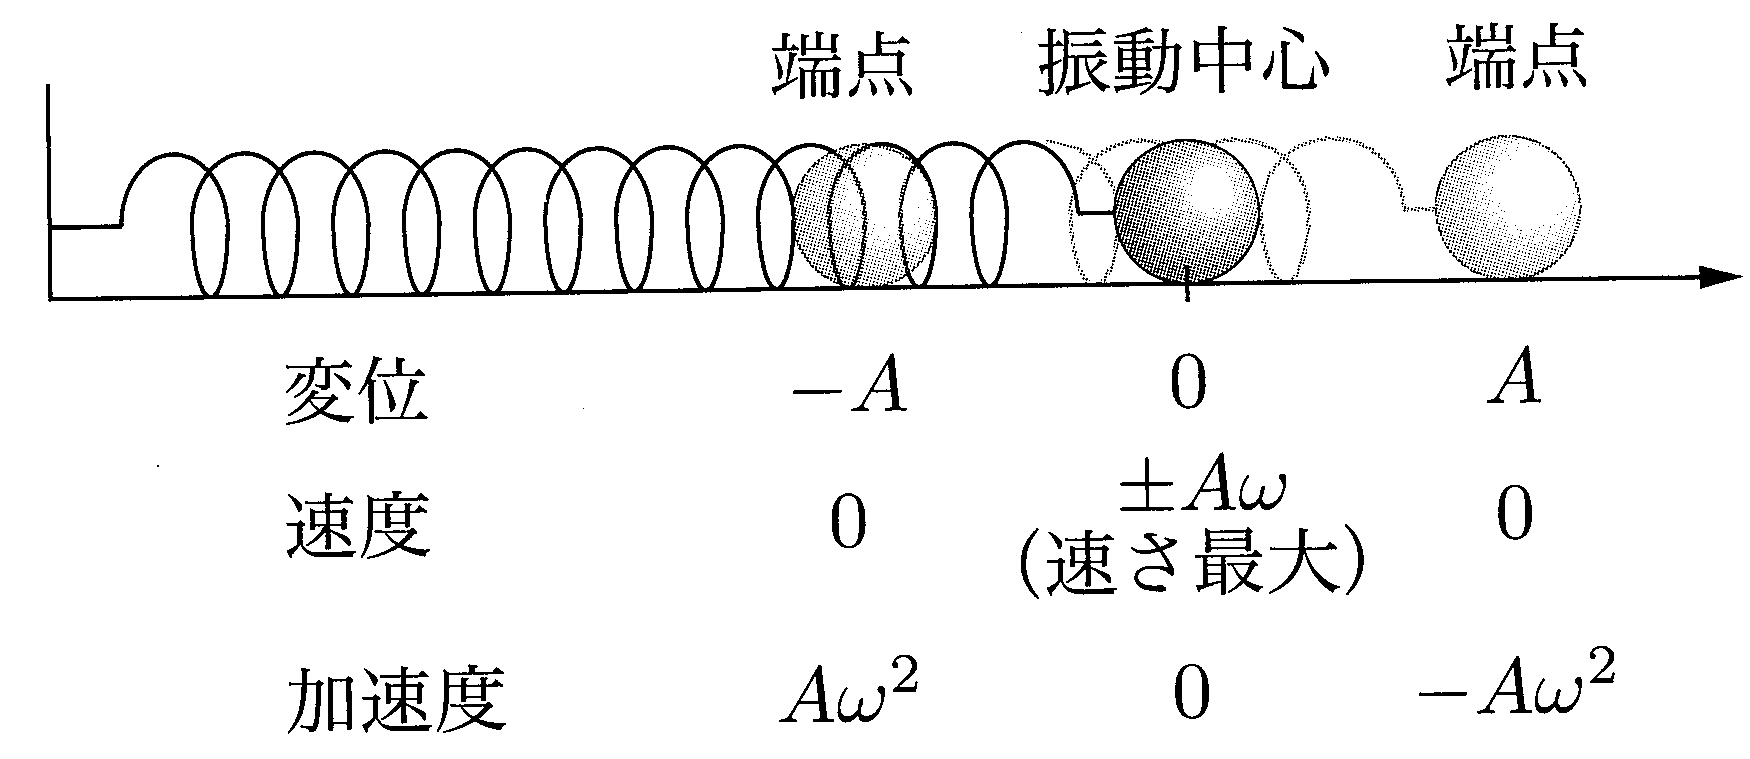
\includegraphics[width=80mm]{text_p40_fig1.png}
%\end{center}
%\end{figure}


 
なお，単振動の式$x=A\sin (\omega t+\varphi_0) $の$A,\varphi_0$はどのような定数値でも元の運動方程式$ma=-kx$を満たすことができる．
また逆に，物体の運動方程式が$ma=-kx$の形になる場合の物体の座標$x(t)$は，必ず$x=A\sin (\omega t+\varphi_0)$の形にまとめられることが知られている．
すなわち，{\bf 運動方程式}\mbox{\boldmath $ma=-kx\hspace{3mm}(k>0)$}{\bf を満たすことと，運動が}\mbox{\boldmath $x=A\sin (\omega t+\varphi_0)\hspace{3mm} \left( \omega=\sqrt{\dfrac{k}{m}} \right)$}{\bf で表されることは数学的に等価である．}
 
 よって，運動方程式が$ma=-kx$の形になる物体の座標$x(t)$の式を決めるには，$x=A\sin (\omega t+\varphi_0) $の式の$A,\varphi_0$の値を決めてやればよく，これらは問題文で与えられた条件（初期条件という）によって決める．
 
 また，運動方程式$ma=-kx$に対して，$x=A\sin (\omega t+\varphi_0) $を加法定理で分解した$x=B\sin \omega t+C\cos \omega t \hspace{2mm}（ただしB,Cは任意の定数）$を解として用いて，$BとC$を決定したほうが求めやすい．
 
 \ 
 
 \subsection{重力下における単振動}
 
 \begin{wrapfigure}[18]{r}[5mm]{70mm}
  \centering
  \vspace{-5mm}
  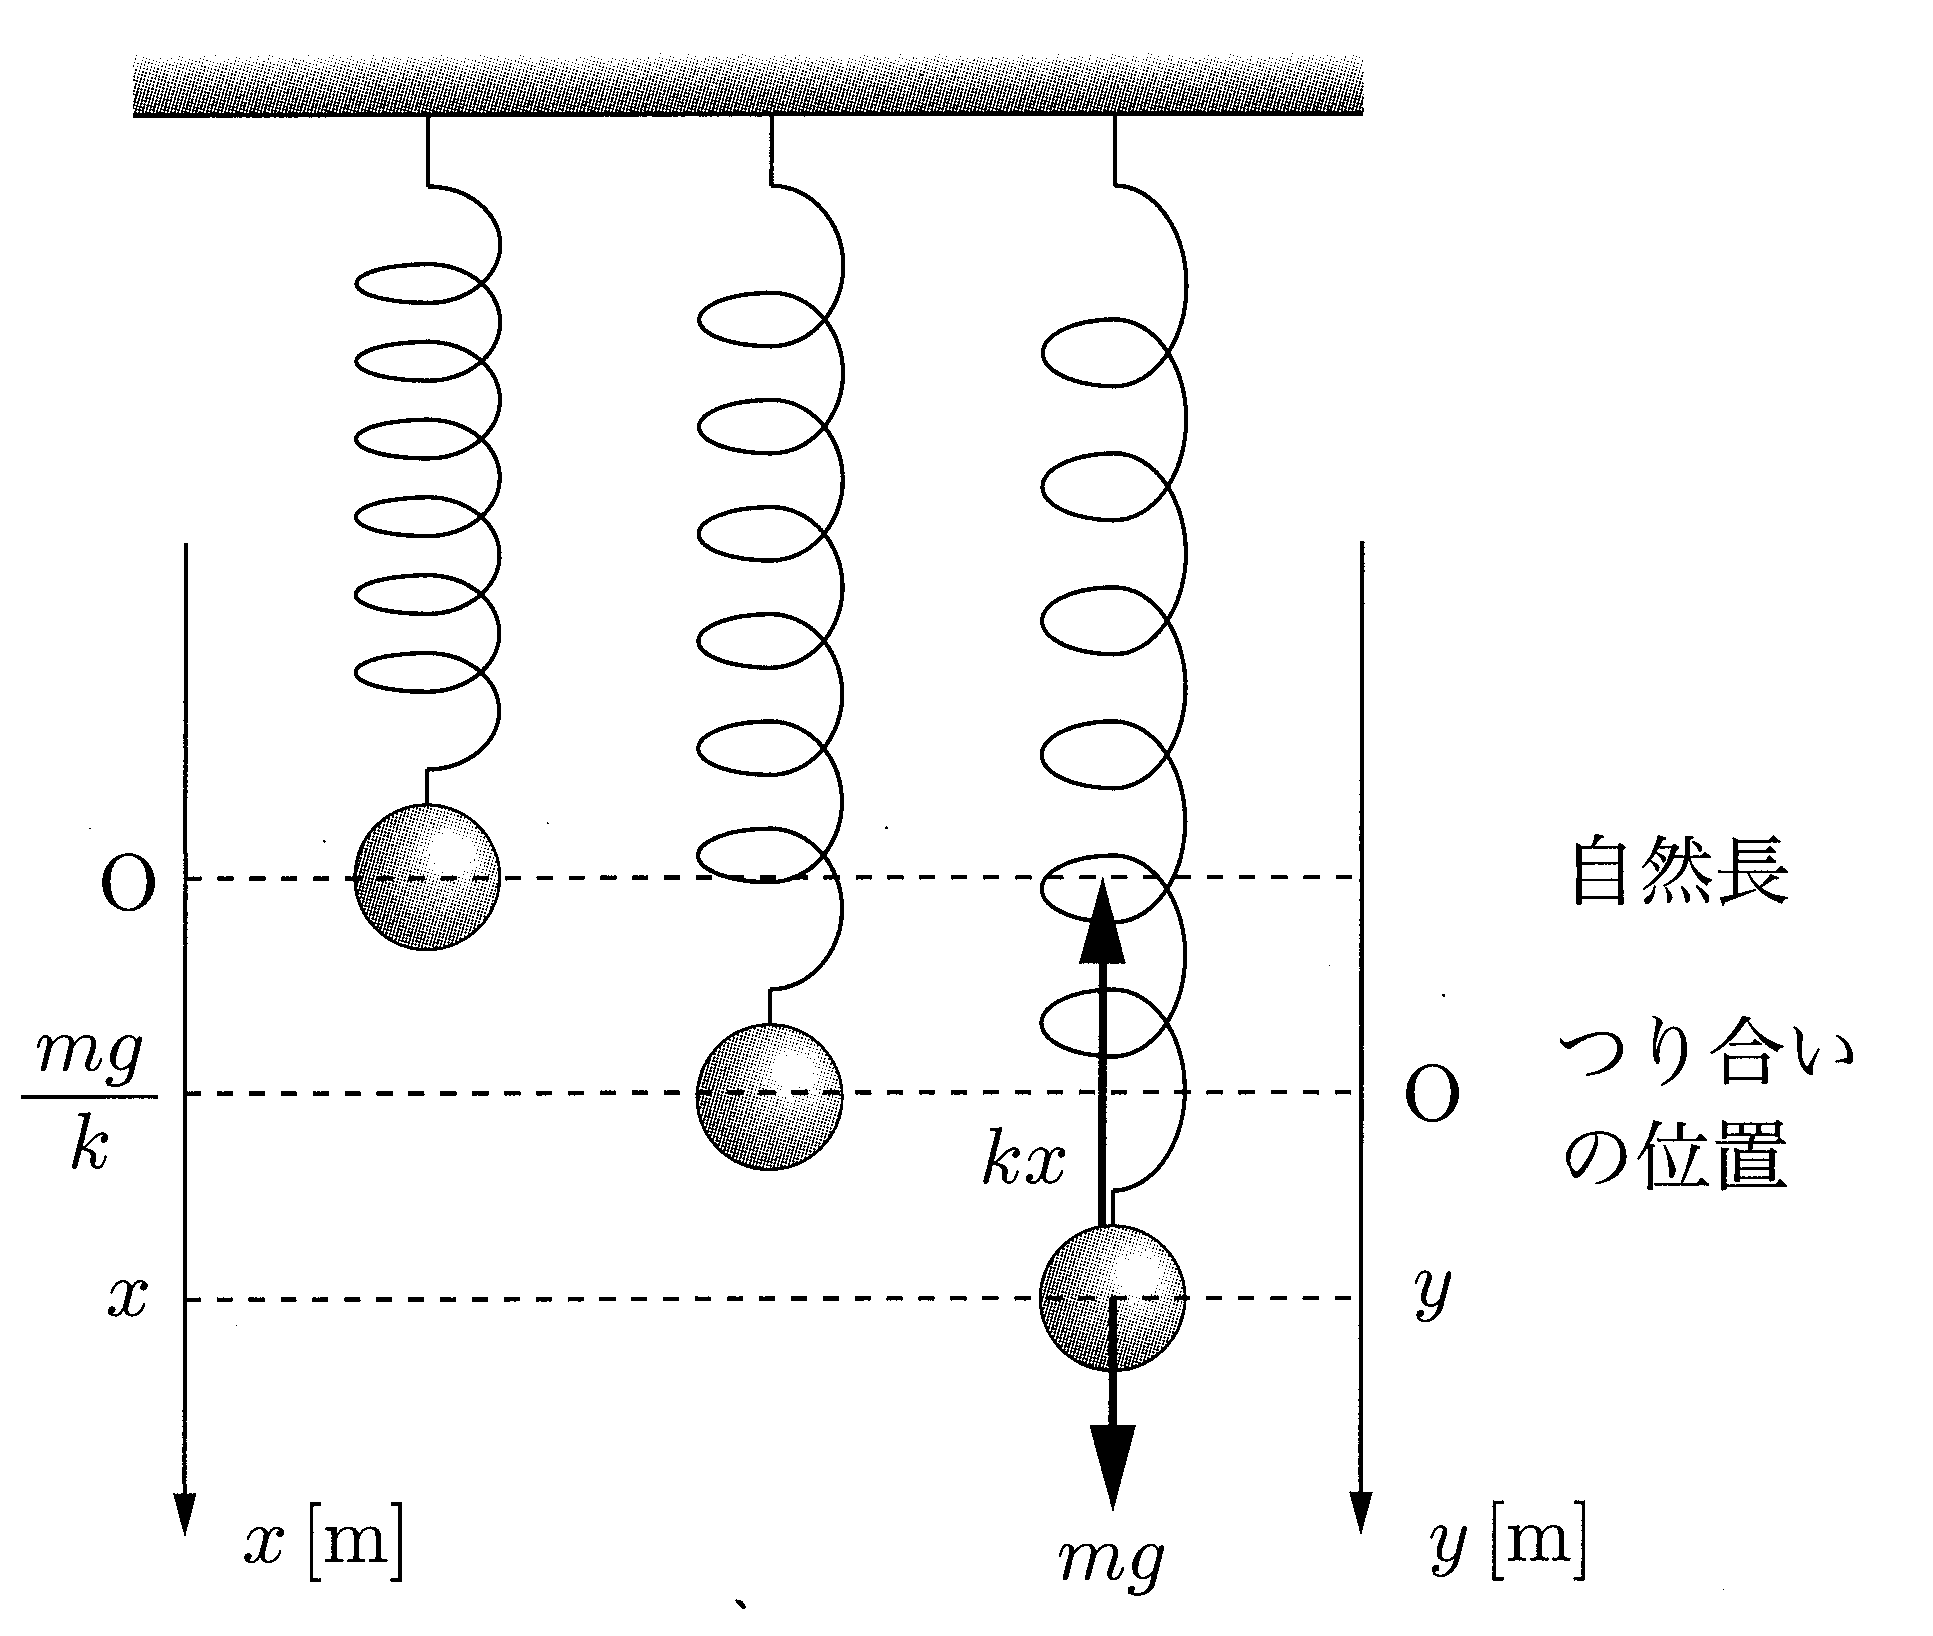
\includegraphics[keepaspectratio,width=70mm]
  {text_p41_fig1.png}
\end{wrapfigure}

 天井から鉛直につるしたバネ定数$k$[N/m]に取り付けた質量$m$[kg]の物体の運動について考える．
 バネが自然長のとき，の物体の位置を原点とし，鉛直下向きに$x$軸をとる．
 バネの弾性力は自然長からの変位に比例することに注意すると，物体が位置$x$[m]にいるときの運動方程式は$x$軸方向（下向き）を正として
 \[ ma=mg-kx\]
 で与えられる．
 これを変形すると，
 \[ ma=-k\left( x-\dfrac{mg}{k} \right)\]
 となるが，ここで$y=x-\dfrac{mg}{k}$なる座標軸$y$を設定すると，上の式は
 \[ ma=-ky\]
 とまとめられる．
 また，$a=\dfrac{d^2x}{dt^2}=\dfrac{d^2y}{dt^2}$であるから，$y$軸上で見ても加速度は$a$である．
 よって，
 \[a=-\dfrac{k}{m}y\]
 より，この物体は$y=0$[m]を中心とし，角振動数$\omega =\sqrt{\dfrac{k}{m}}$[rad/s]の単振動を行うことがわかる．
 この単振動の中心位置$y=0$[m]とは$x=\dfrac{mg}{k}$[m]であり，これは{\bf 物体に作用する重力とバネの弾性力とがつりあう点}である．
 
 \begin{matome}{重力下での単振動}
 \hspace{5mm} 自然長の位置を基準とした運動方程式を変形して
 \[ ma=-k(x-x_0) \]
 \hspace{5mm} の形にまとめ，振動中心$x=x_0$[m]（力のつり合いの位置），角振動数$\omega=\sqrt{\dfrac{k}{m}}$[rad/s]を求める．
 \end{matome}
 
  
 \ 
 
%\begin{breakbox}
%\ex＜重力下における単振動＞\\
%\begin{wrapfigure}[7]{r}[5mm]{50mm}
%  \centering
%  \vspace{-5mm}
%  \includegraphics[keepaspectratio,width=40mm]
%  {text_p42_fig1.png}
%\end{wrapfigure}
%\hspace{5mm}天井から鉛直につるしたばね定数$k$[N/m]のバネに取り付けた質量$m$[kg]の物体の運動について考える．
%バネが自然長のときの位置を$x$軸の原点とし，鉛直下向きに正の向きをとる．
%今，物体を自然長位置で軽く支えておき，時刻$t=0$[s]にそっと手を離した．
%重力加速度の大きさを$g {\rm [m/s^2]}$として以下の問いに答えよ．
%\begin{description}
%\item[(1)] 物体が位置$x$[m]にあるときの物体の運動方程式を示せ．
%\item[(2)] この単振動の中心位置$x_0$[m]および角振動数$\omega$[rad/s]を求めよ．
%\item[(3)] この単振動の振幅$A$[m]を求めよ．
%\item[(4)] 物体が達する最下点の座標$x_1$[m]を求めよ．
%\item[(5)] 物体が振動中心を通過する速さ$v_0$[m/s]を求めよ．
%\item[(6)] この物体の任意の時刻$t$[s]における位置を，時刻$t$の関数として表せ．
%\end{description}
%
%\end{breakbox}

 \ 
 
%  \newpage
 \subsection{単振動のまとめ}
 
 単振動の特徴をまとめると以下のようになる．
 
 \begin{matome}{単振動のまとめ}
 \hspace{5mm} ・『運動方程式$ma=-k(x-x_0)\hspace{3mm} (k>0)$で表せる』\\
 \hspace{20mm} $\Leftrightarrow 『x=x_0+A\sin (\omega t+\varphi_0) で表される単振動を行う』$\\
 \hspace{5mm} ・振動中心$x=x_0$\hspace{3mm} 角振動数$\omega =\sqrt{\dfrac{k}{m}}$ \hspace{3mm} 周期$T=\dfrac{2\pi}{\omega}$\\
  \hspace{5mm} ・単振動の振動中心は力のつり合いの位置となる．\\
  \hspace{5mm} ・振動中心で速さが最大となり，$v_{max}=A\omega$[m/s]\\
  \hspace{5mm} ・加速度が最大となるのは振動端点．
 \end{matome} 
 
重力下に限らず，つり合いの位置からの変位に比例して復元力（つり合いの位置に戻そうとする力）が作用する場合には単振動を行う．
一般に単振動についての解き方をまとめると以下の通りとなる．

 
 \begin{matome}{単振動の解法}
 \hspace{3mm} $\MARU{1}$\hspace{2mm}位置$x$\hspace{1mm}[m]において物体に作用している力を描き出し，運動方程式を立てる．\\
 \hspace{10mm} $\underline{ポイント}$ ・特定の位置ではなく，任意の位置$x$[m]で考える．\\
  \hspace{24mm}  ・加速度$a=\dfrac{d^2x}{dt^2} \hspace{1mm} {\rm [m/s^2]}$の向きは$x$軸と同じ向きに設定する．\\
  \hspace{24mm}  ・複数物体がある場合は各物体ごとに別々に立てればよい．\\
 \hspace{3mm} $\MARU{2}$\hspace{2mm}式変形して$ma=-k(x-x_0)$の形を作り，角振動数$\omega=\sqrt{\dfrac{k}{m}}$\hspace{1mm}[rad/s]，振動中心$x_0$[m]を求める．\\
 \hspace{10mm} $\underline{ポイント}$ ・$k$および$x_0$は時刻や位置によらない定数になるように変形する．\\
  \hspace{24mm}  ・$k$が正の場合のみ単振動となる．\\
  \hspace{24mm}  ・複数物体があり，垂直抗力や張力など未知数が含まれる場合には連立して未知数を\\ \hspace{28mm}消去してこの形を目指す．\\
   \hspace{3mm} $\MARU{3}$\hspace{2mm}必要に応じて初期条件から振幅$A$\hspace{1mm}[m]および初期位相$\varphi$を求める．\\
 \hspace{10mm} $\underline{ポイント}$ ・速度が0\hspace{1mm}[m/s]の位置が与えられていれば（そっと手を離した，など），\\ \hspace{28mm}その位置が端点なので，端点と振動中心の距離が振幅となる．\\
  \hspace{24mm}  ・振動中心での速度が与えられていれば$v_{max}=A\omega $を利用して振幅を求める\\ \hspace{28mm}ことができる．\\
  \hspace{24mm}  ・それ以外の位置での速度が与えられている場合はエネルギー保存則を利用して\\ \hspace{28mm}計算して振幅を求める．\\
  \hspace{24mm}  ・時刻$t$における位置を求める場合は，物体の時間変化をグラフに描いた上で\\ \hspace{28mm}数式化するとよい．
 \end{matome} 
 

 \ 
 
%\begin{breakbox}
%\ex＜鉛直方向のバネによる単振動＞\\
%\begin{wrapfigure}[7]{r}[5mm]{70mm}
%  \centering
%  \vspace{-5mm}
%  \includegraphics[keepaspectratio,width=60mm]
%  {text_p43_fig1.png}
%\end{wrapfigure}
%\hspace{5mm}軽いバネの一端を地面に固定して鉛直に立て，他端に質量$M$[kg]の板を取り付け，板の上に質量$m$[kg]の小球を乗せたところ，板は自然長の位置から距離$d$[m]だけ縮んだ位置でつり合った．
%バネをさらに$2d$[m]だけ押し縮めてそっと手を離した．
%この後の運動について以下の問いに答えよ．
%ただし重力加速度の大きさを$g {\rm [m/s^2]}$とする．
%\begin{description}
%\item[(1)] このバネの弾性定数$k$[N/m]を求めよ．
%\item[(2)] 小球と板とが接触している間について，この単振動の周期$T$[s]を求めよ．
%\item[(3)] 手を離してから小球と板がつり合いの位置に戻るのにかかる時間を求めよ．
%\item[(4)] つり合いの位置を通過する瞬間の小球と板の速さを求めよ．
%\item[(5)] 小球が板から離れる位置を求めよ．
%\item[(6)] 手を離してから小球が板から離れるまでにかかる時間を求めよ．
%\end{description}
%
%\end{breakbox}

 \ 
 
 
  \newpage

\begin{figure}[h]
\begin{center}
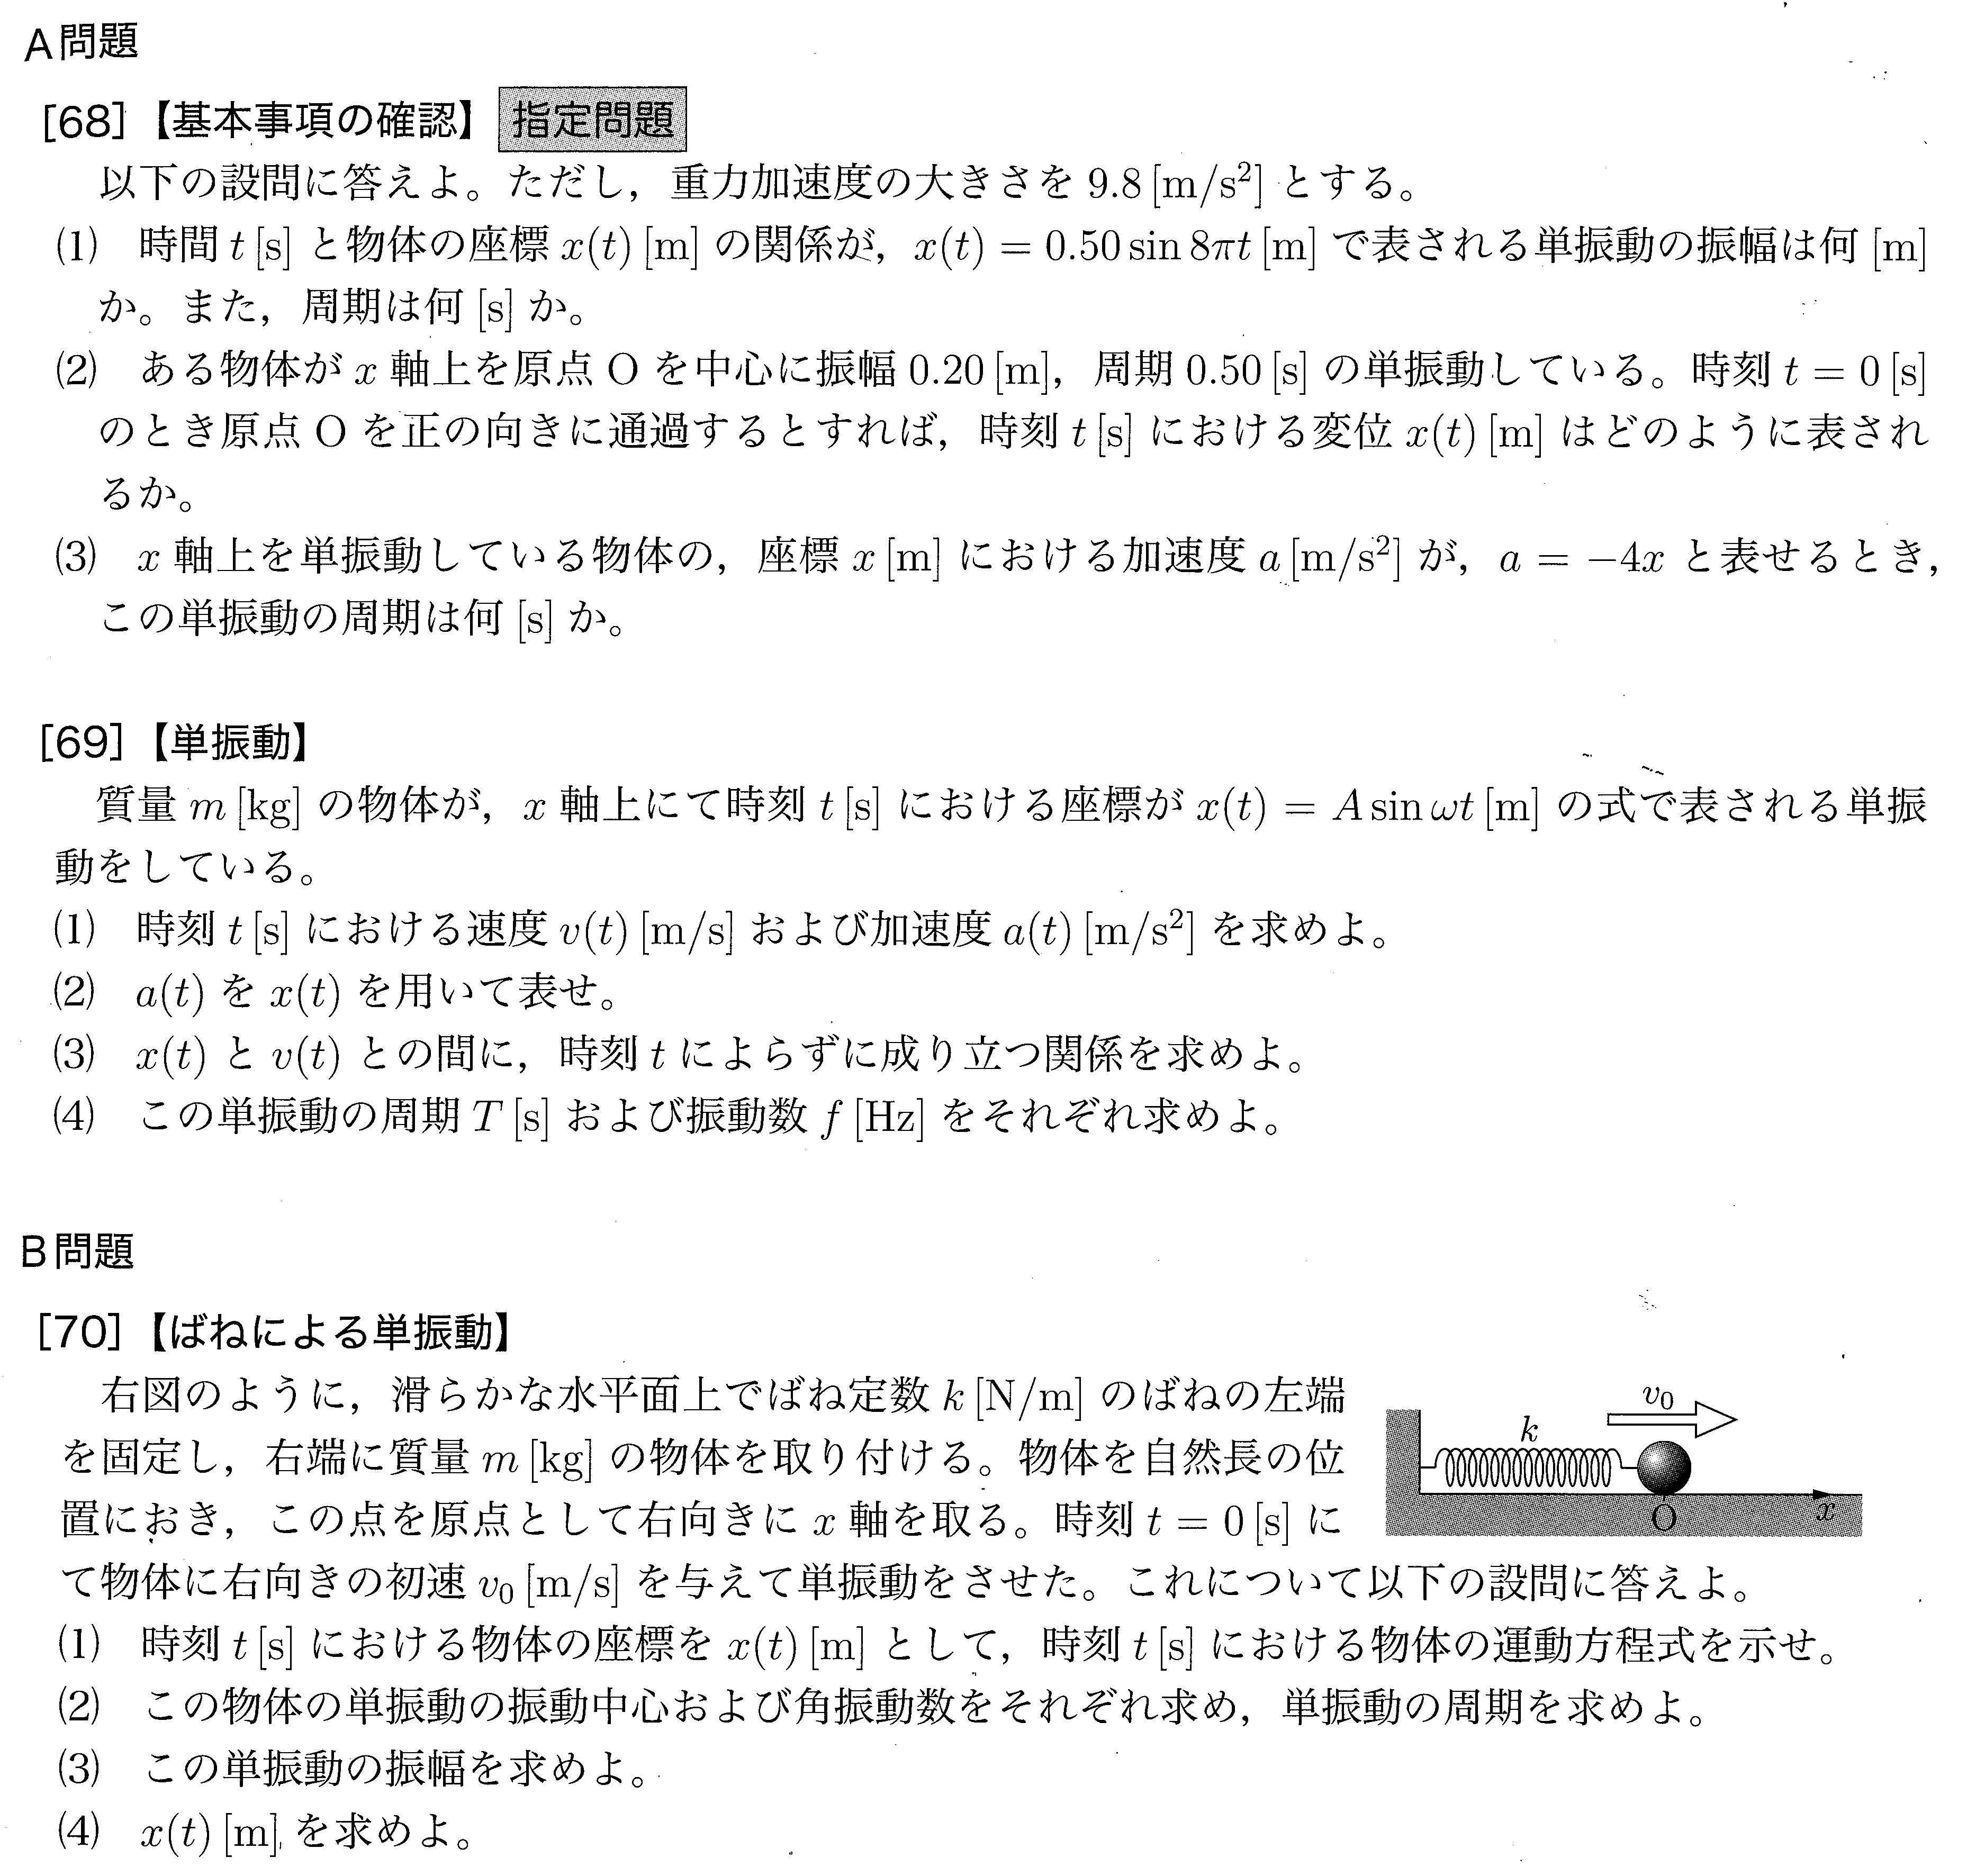
\includegraphics[width=170mm]{prob_p23.png}
\end{center}
\end{figure}

\newpage

\begin{figure}[h]
\begin{center}
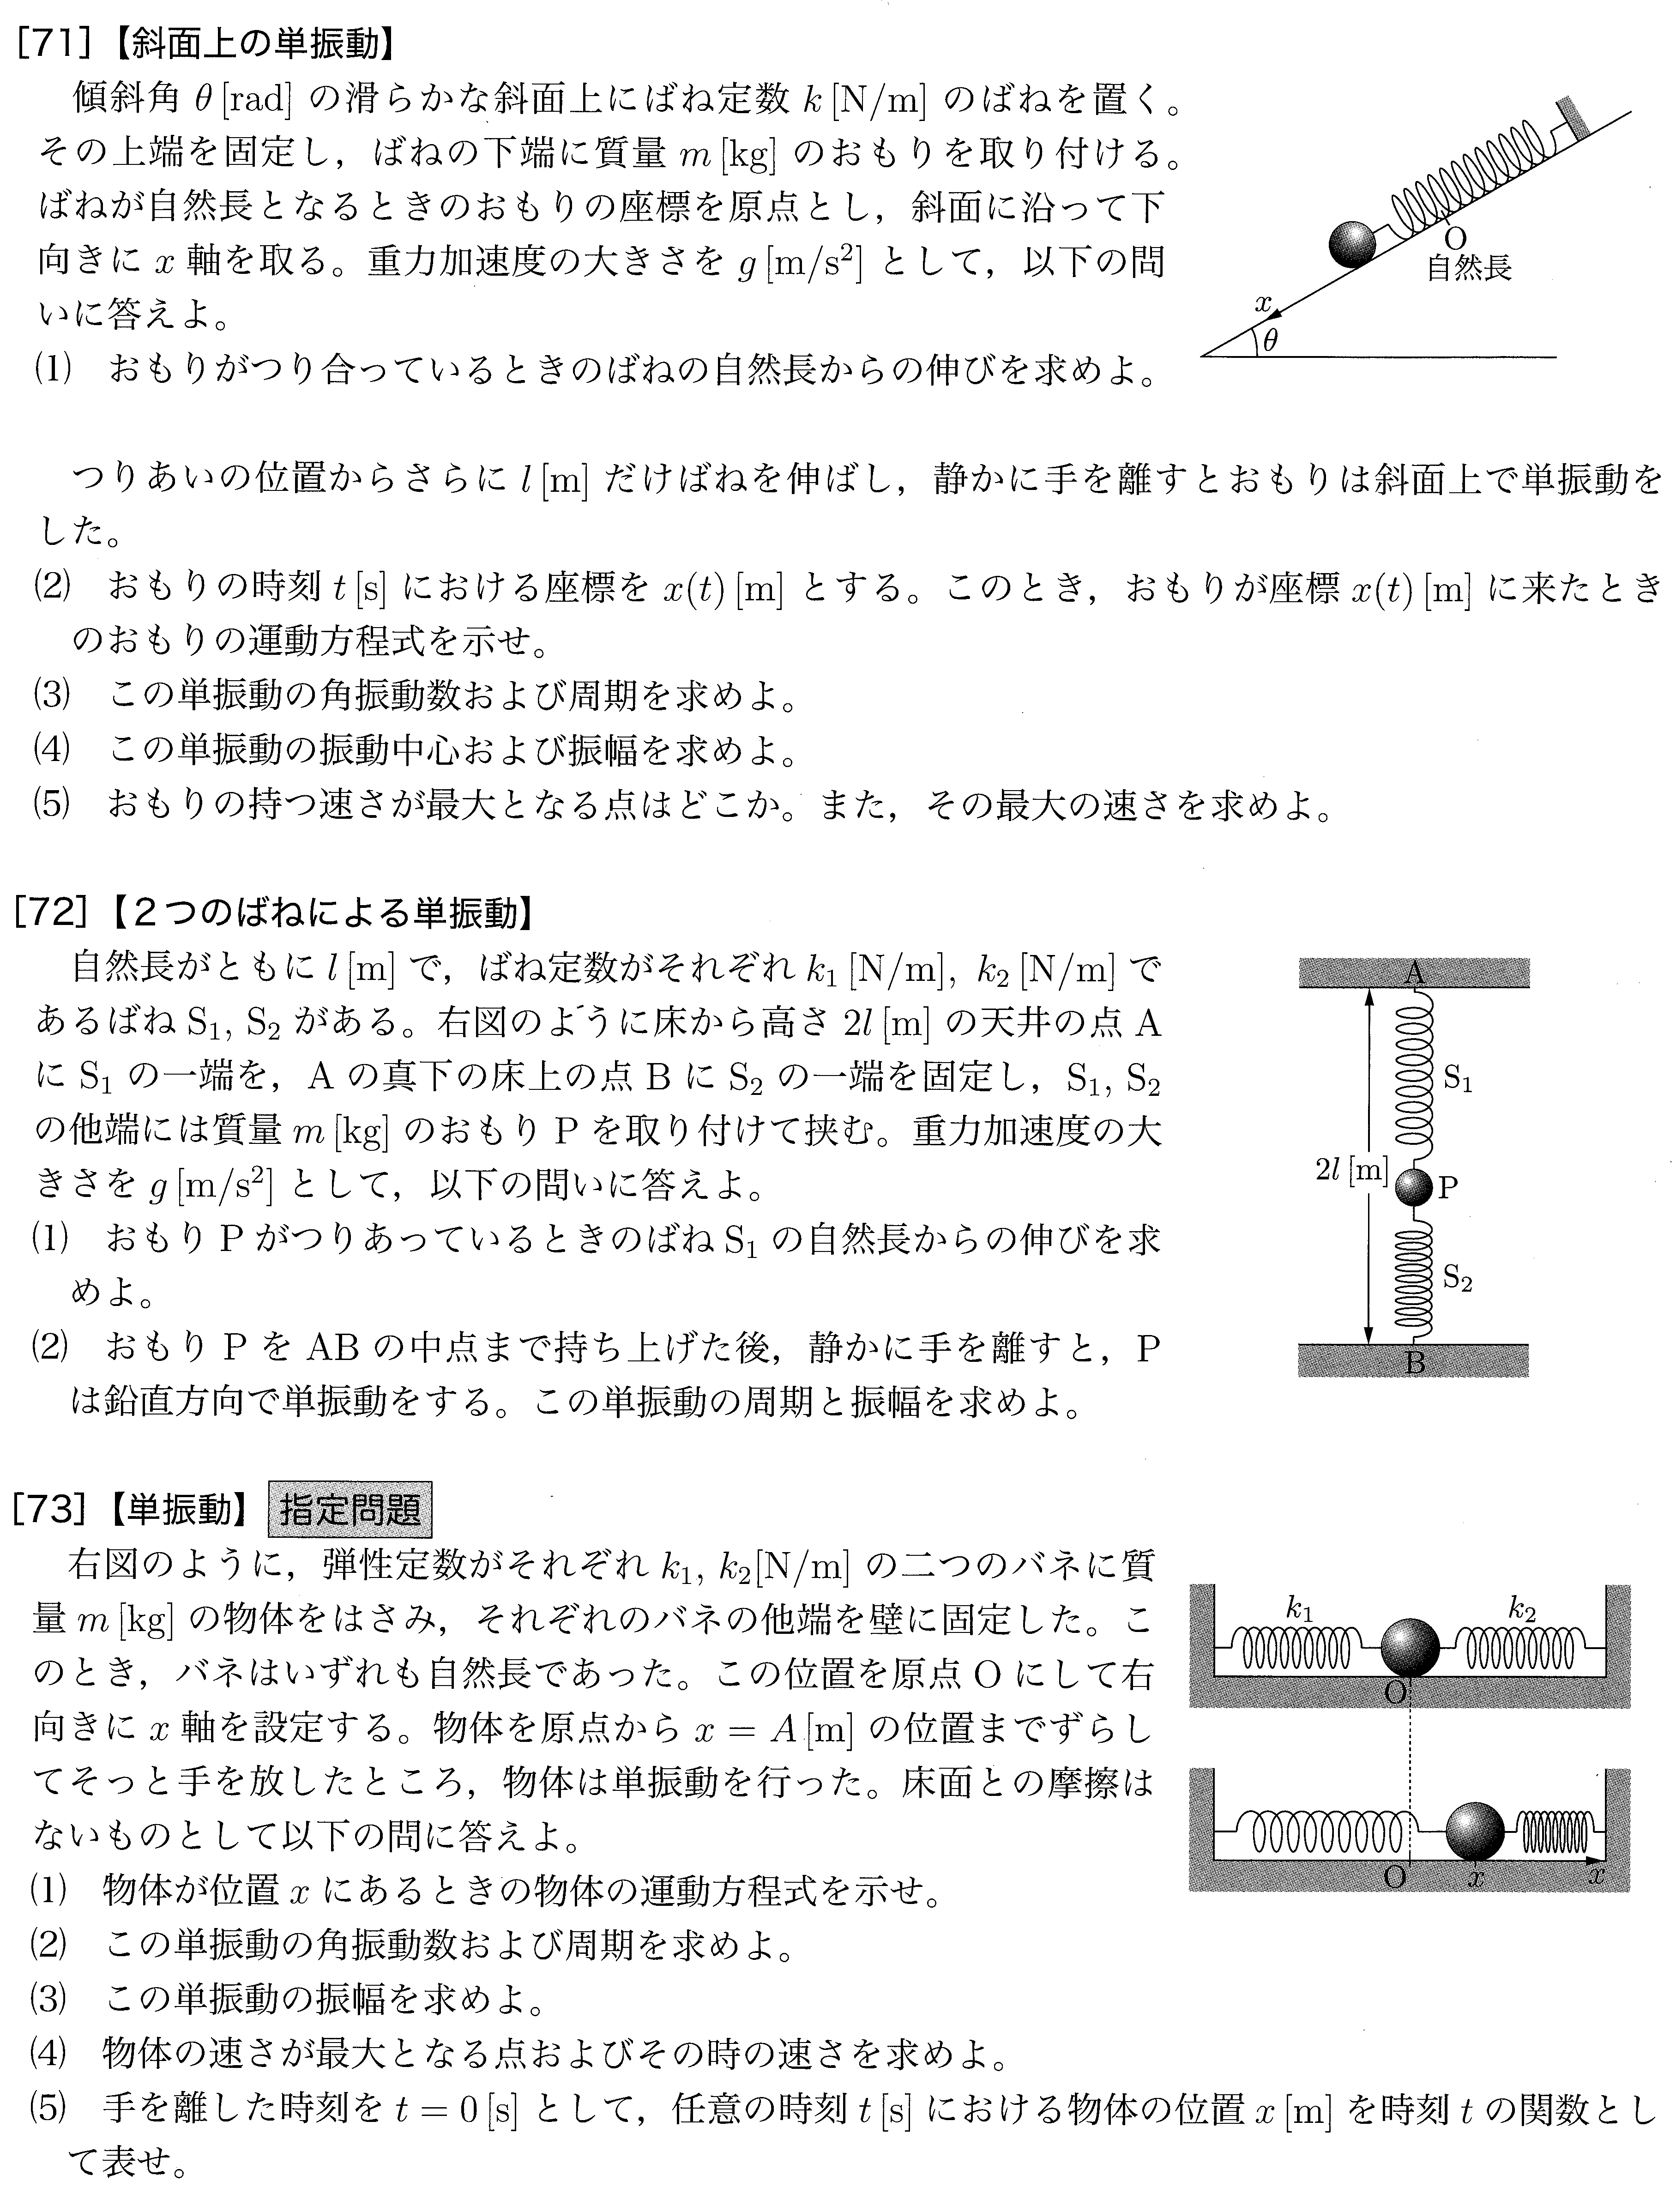
\includegraphics[width=170mm]{prob_p24.png}
\vspace{10cm}
\end{center}
\end{figure}



\newpage

\begin{figure}[h]
\begin{center}
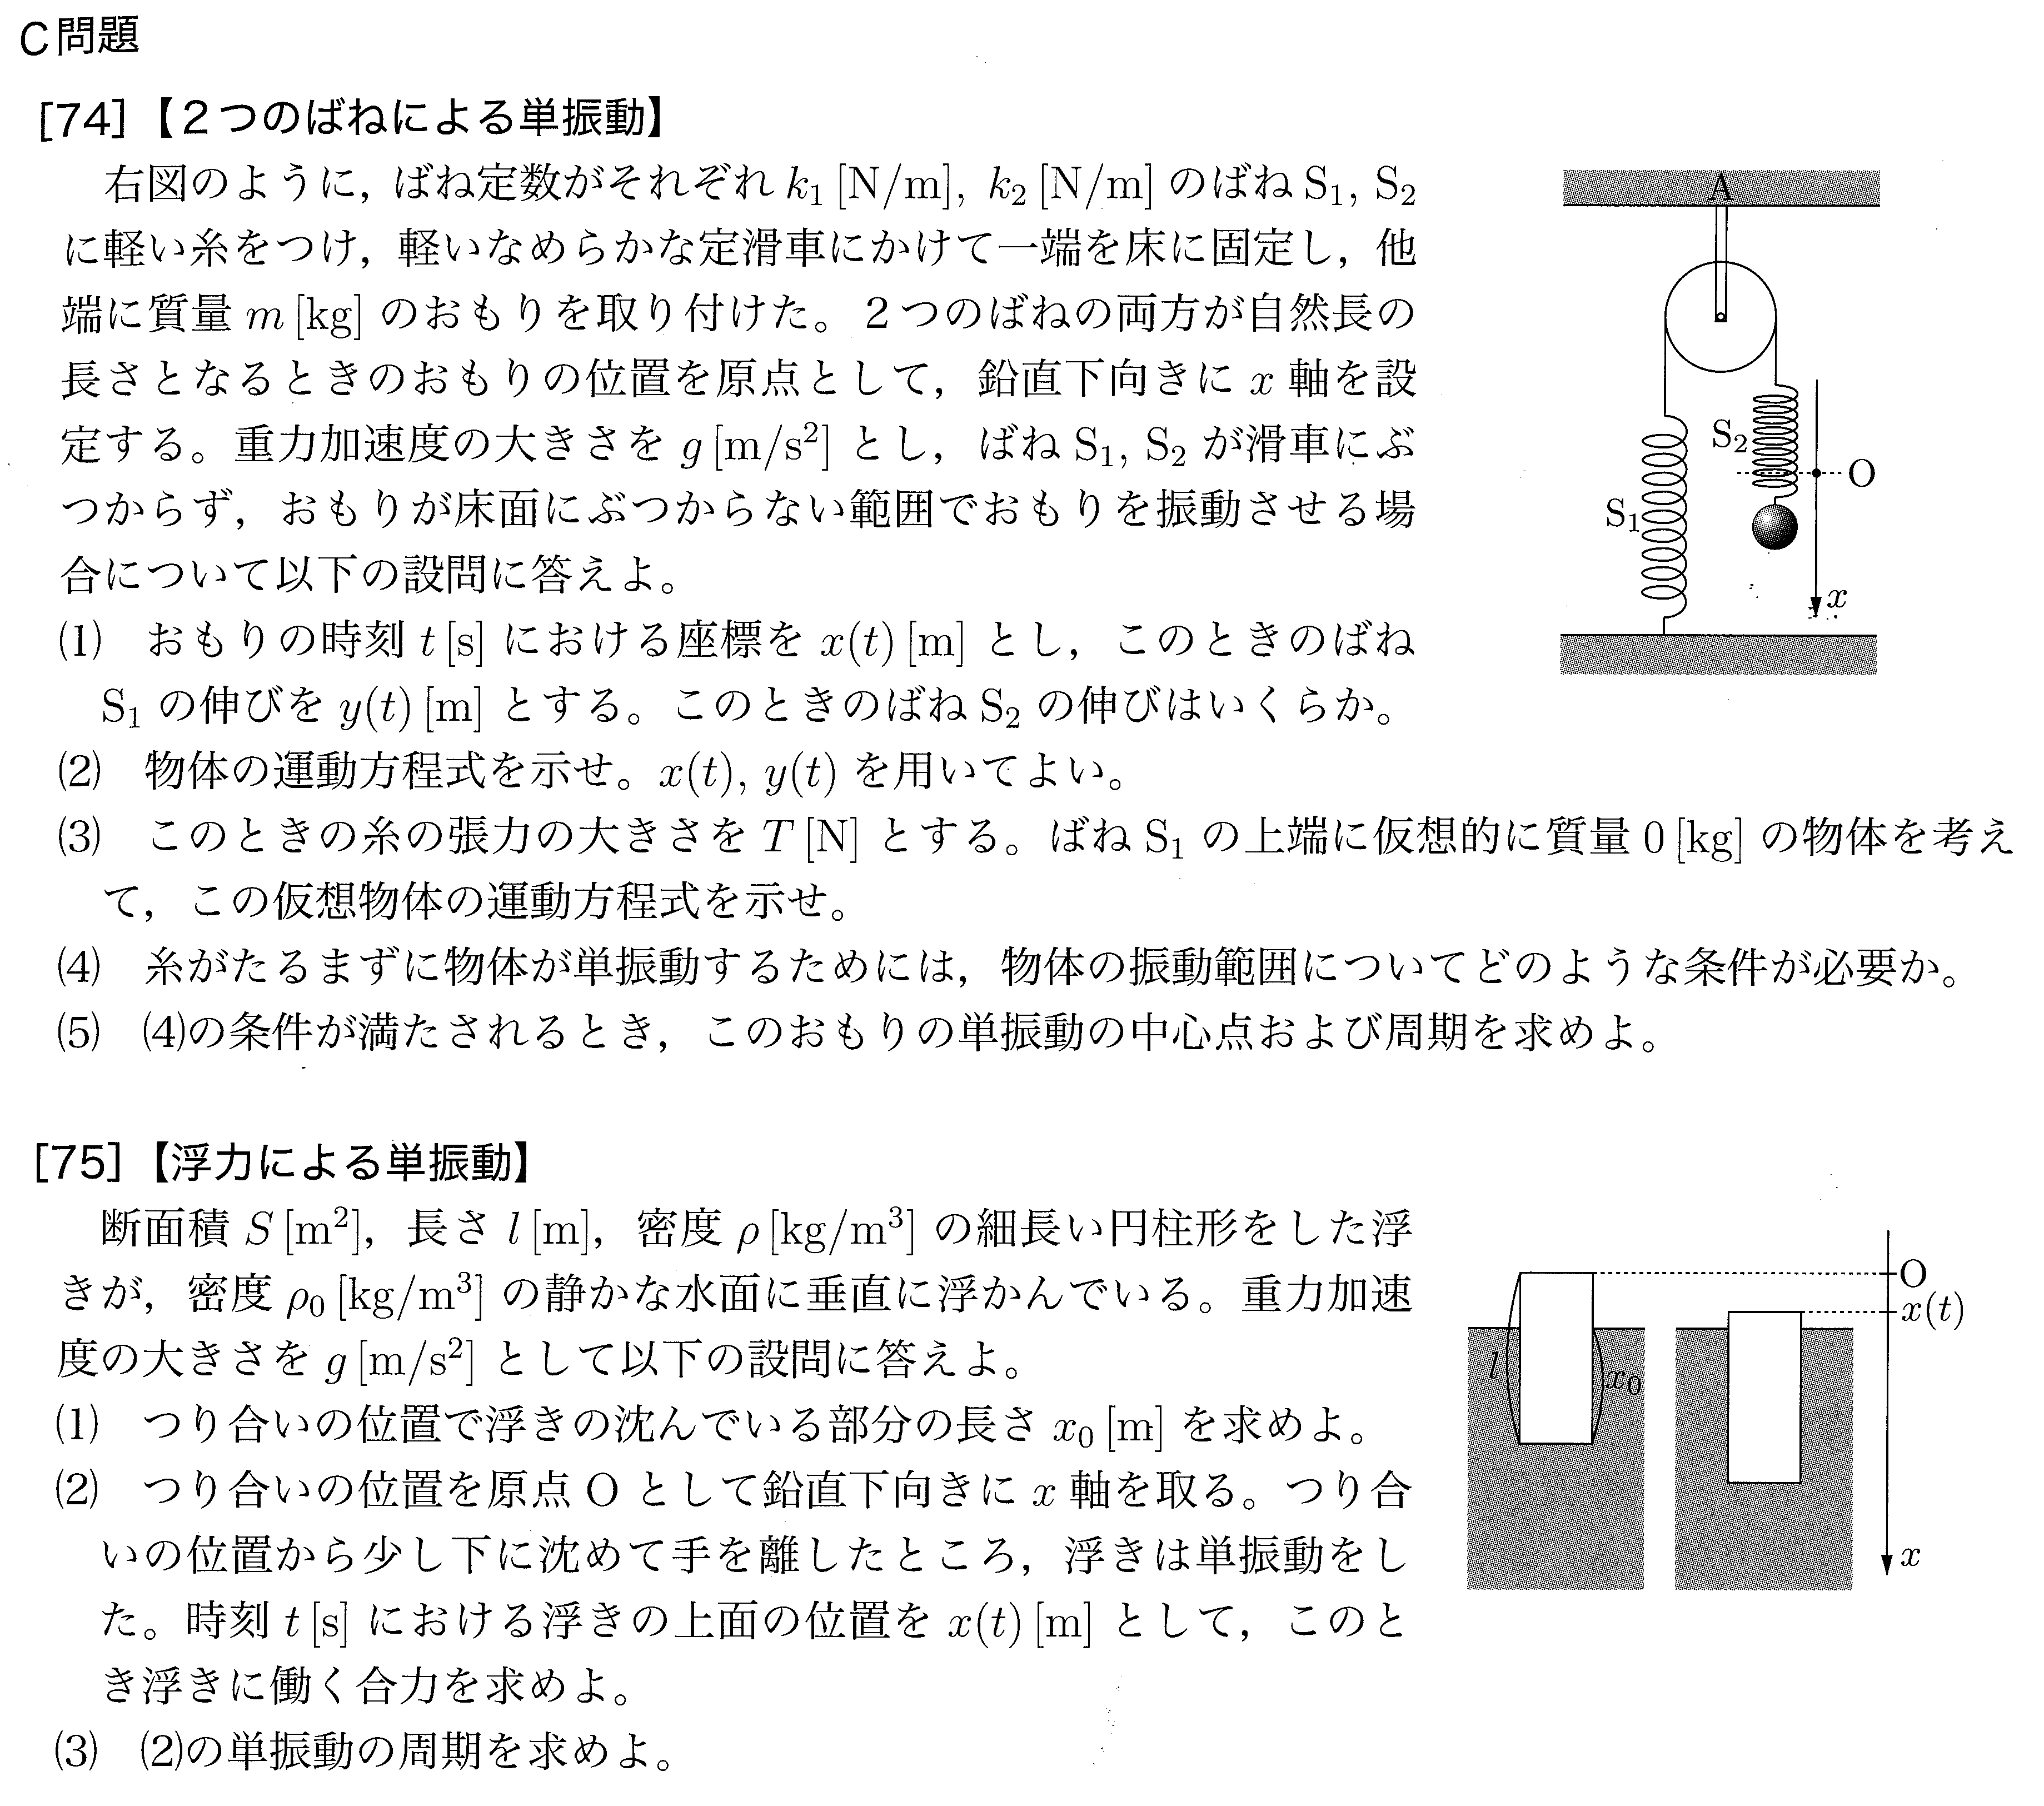
\includegraphics[width=170mm]{prob_p25.png}
\vspace{10cm}
\end{center}
\end{figure}

\newpage

\begin{figure}[h]
\begin{center}
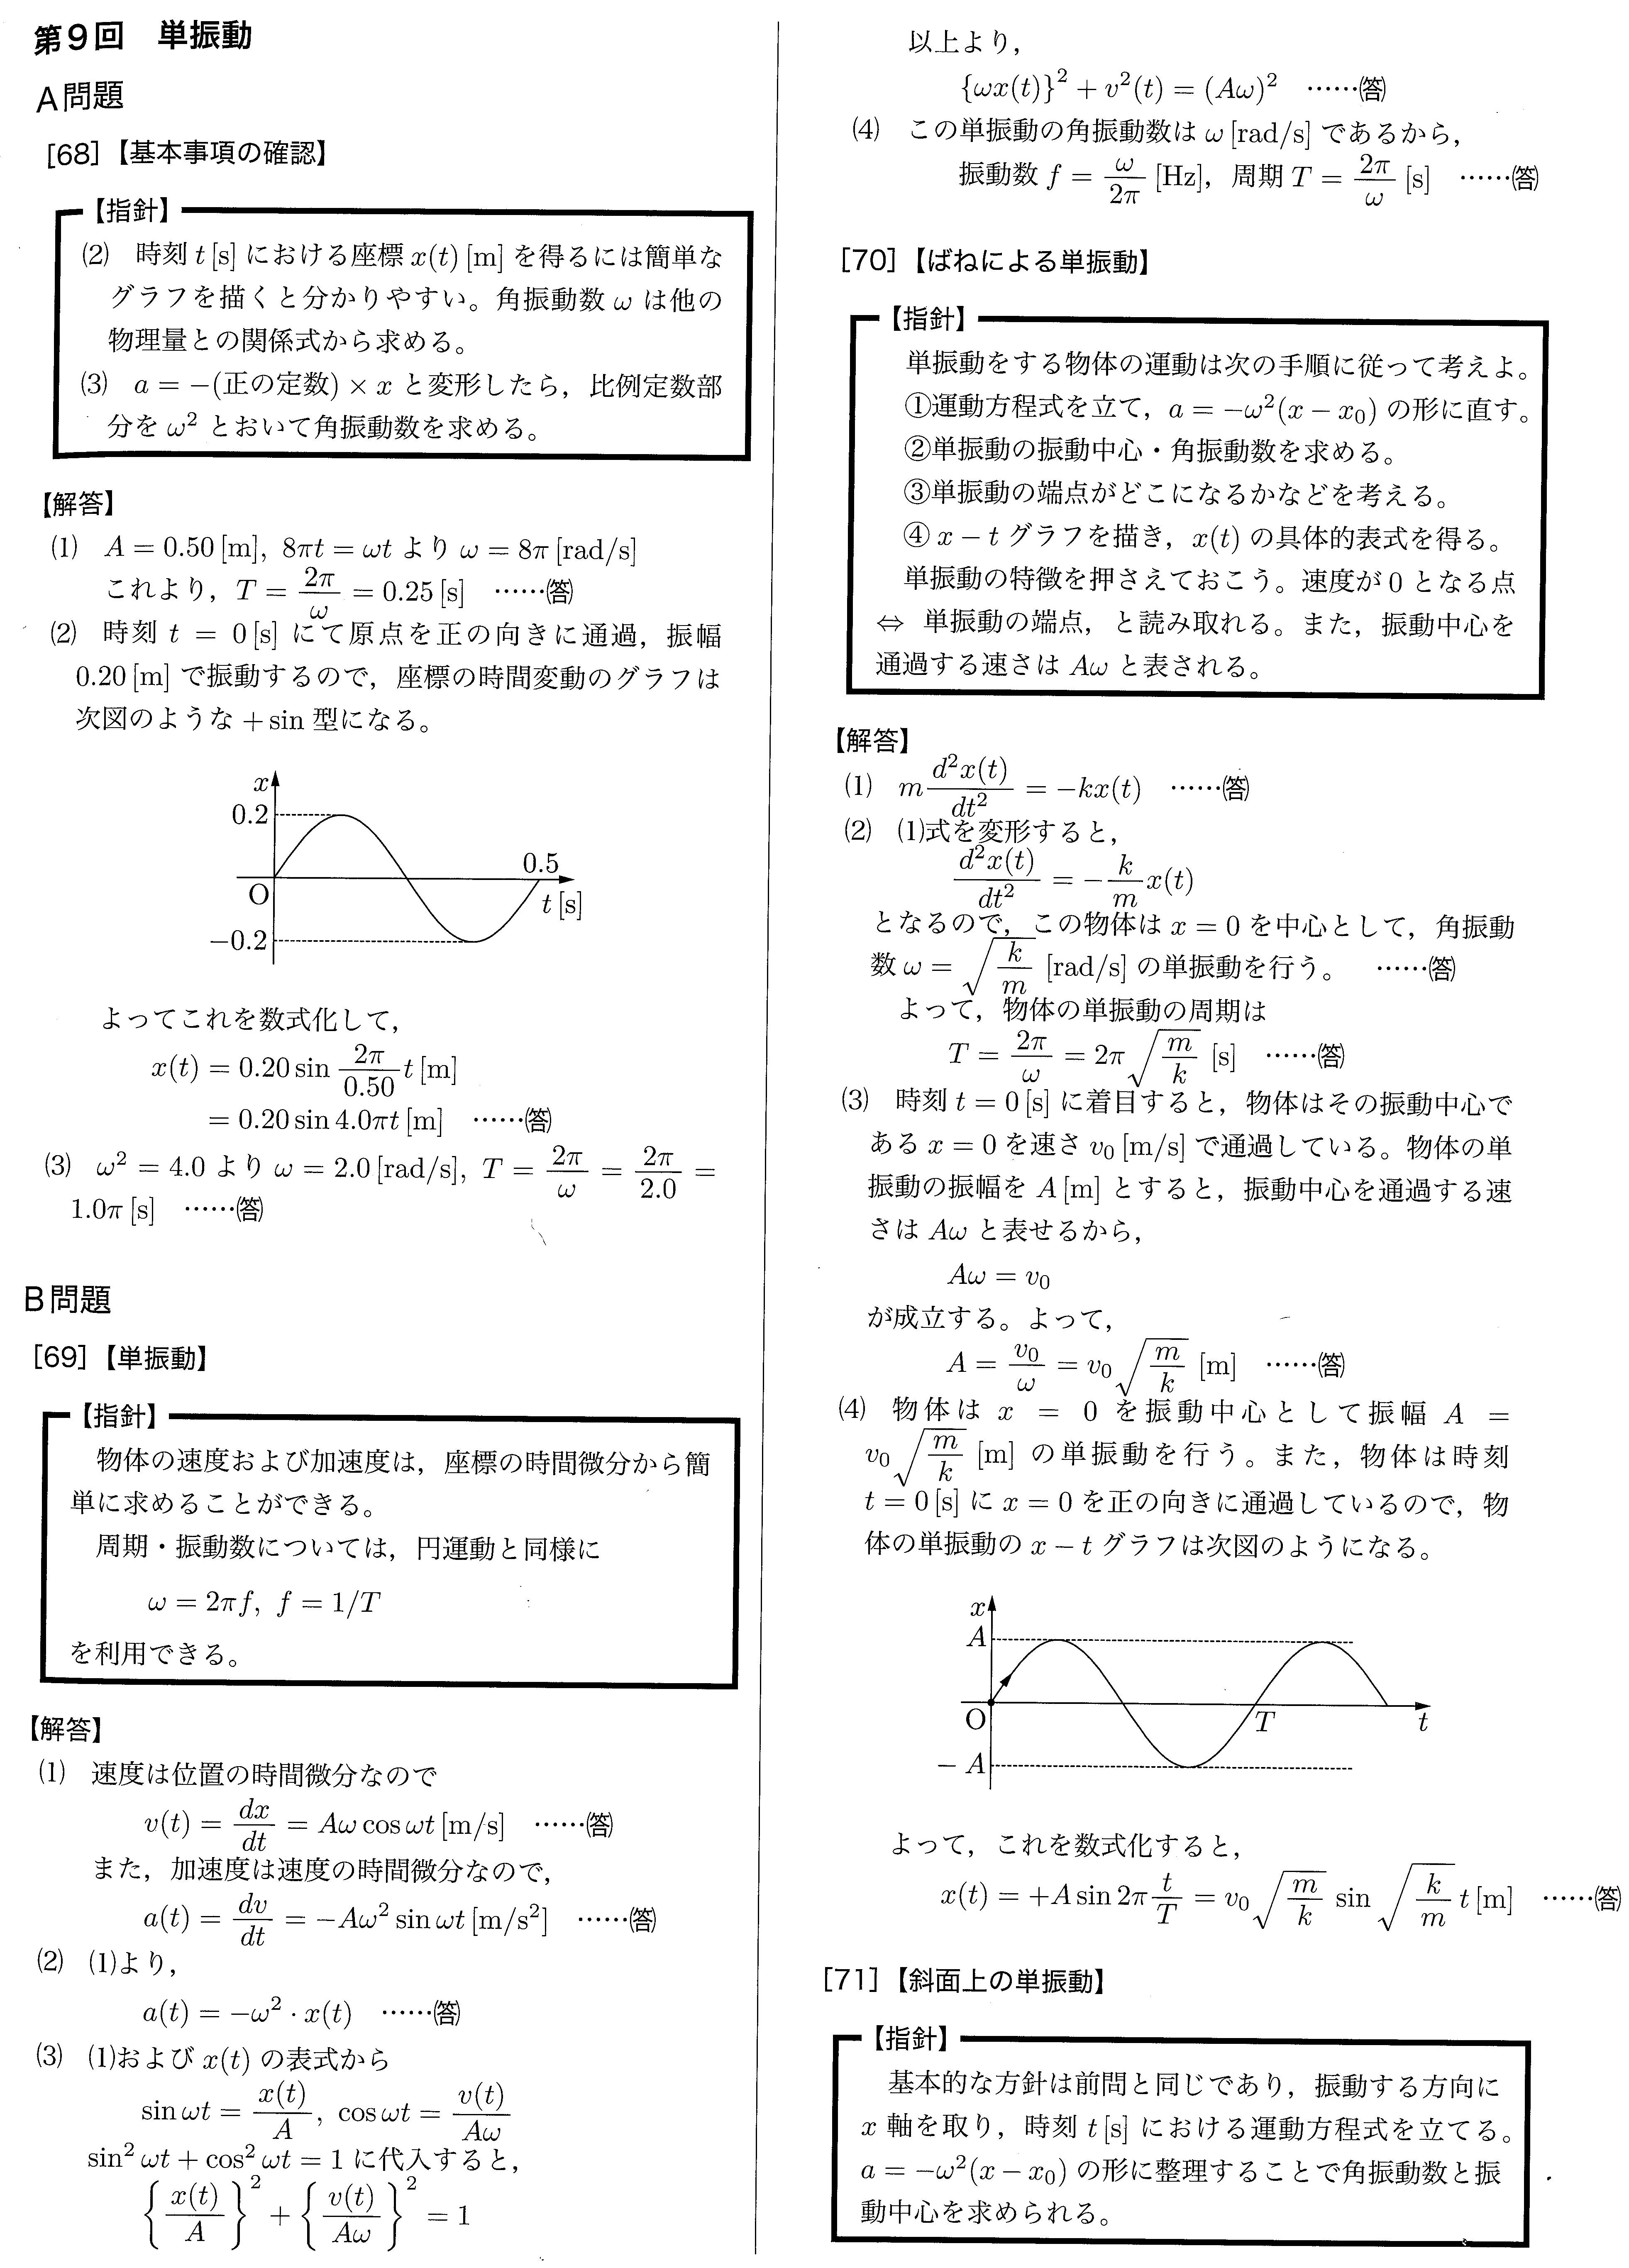
\includegraphics[width=170mm]{prob_p95.png}
\end{center}
\end{figure}

\newpage

\begin{figure}[h]
\begin{center}
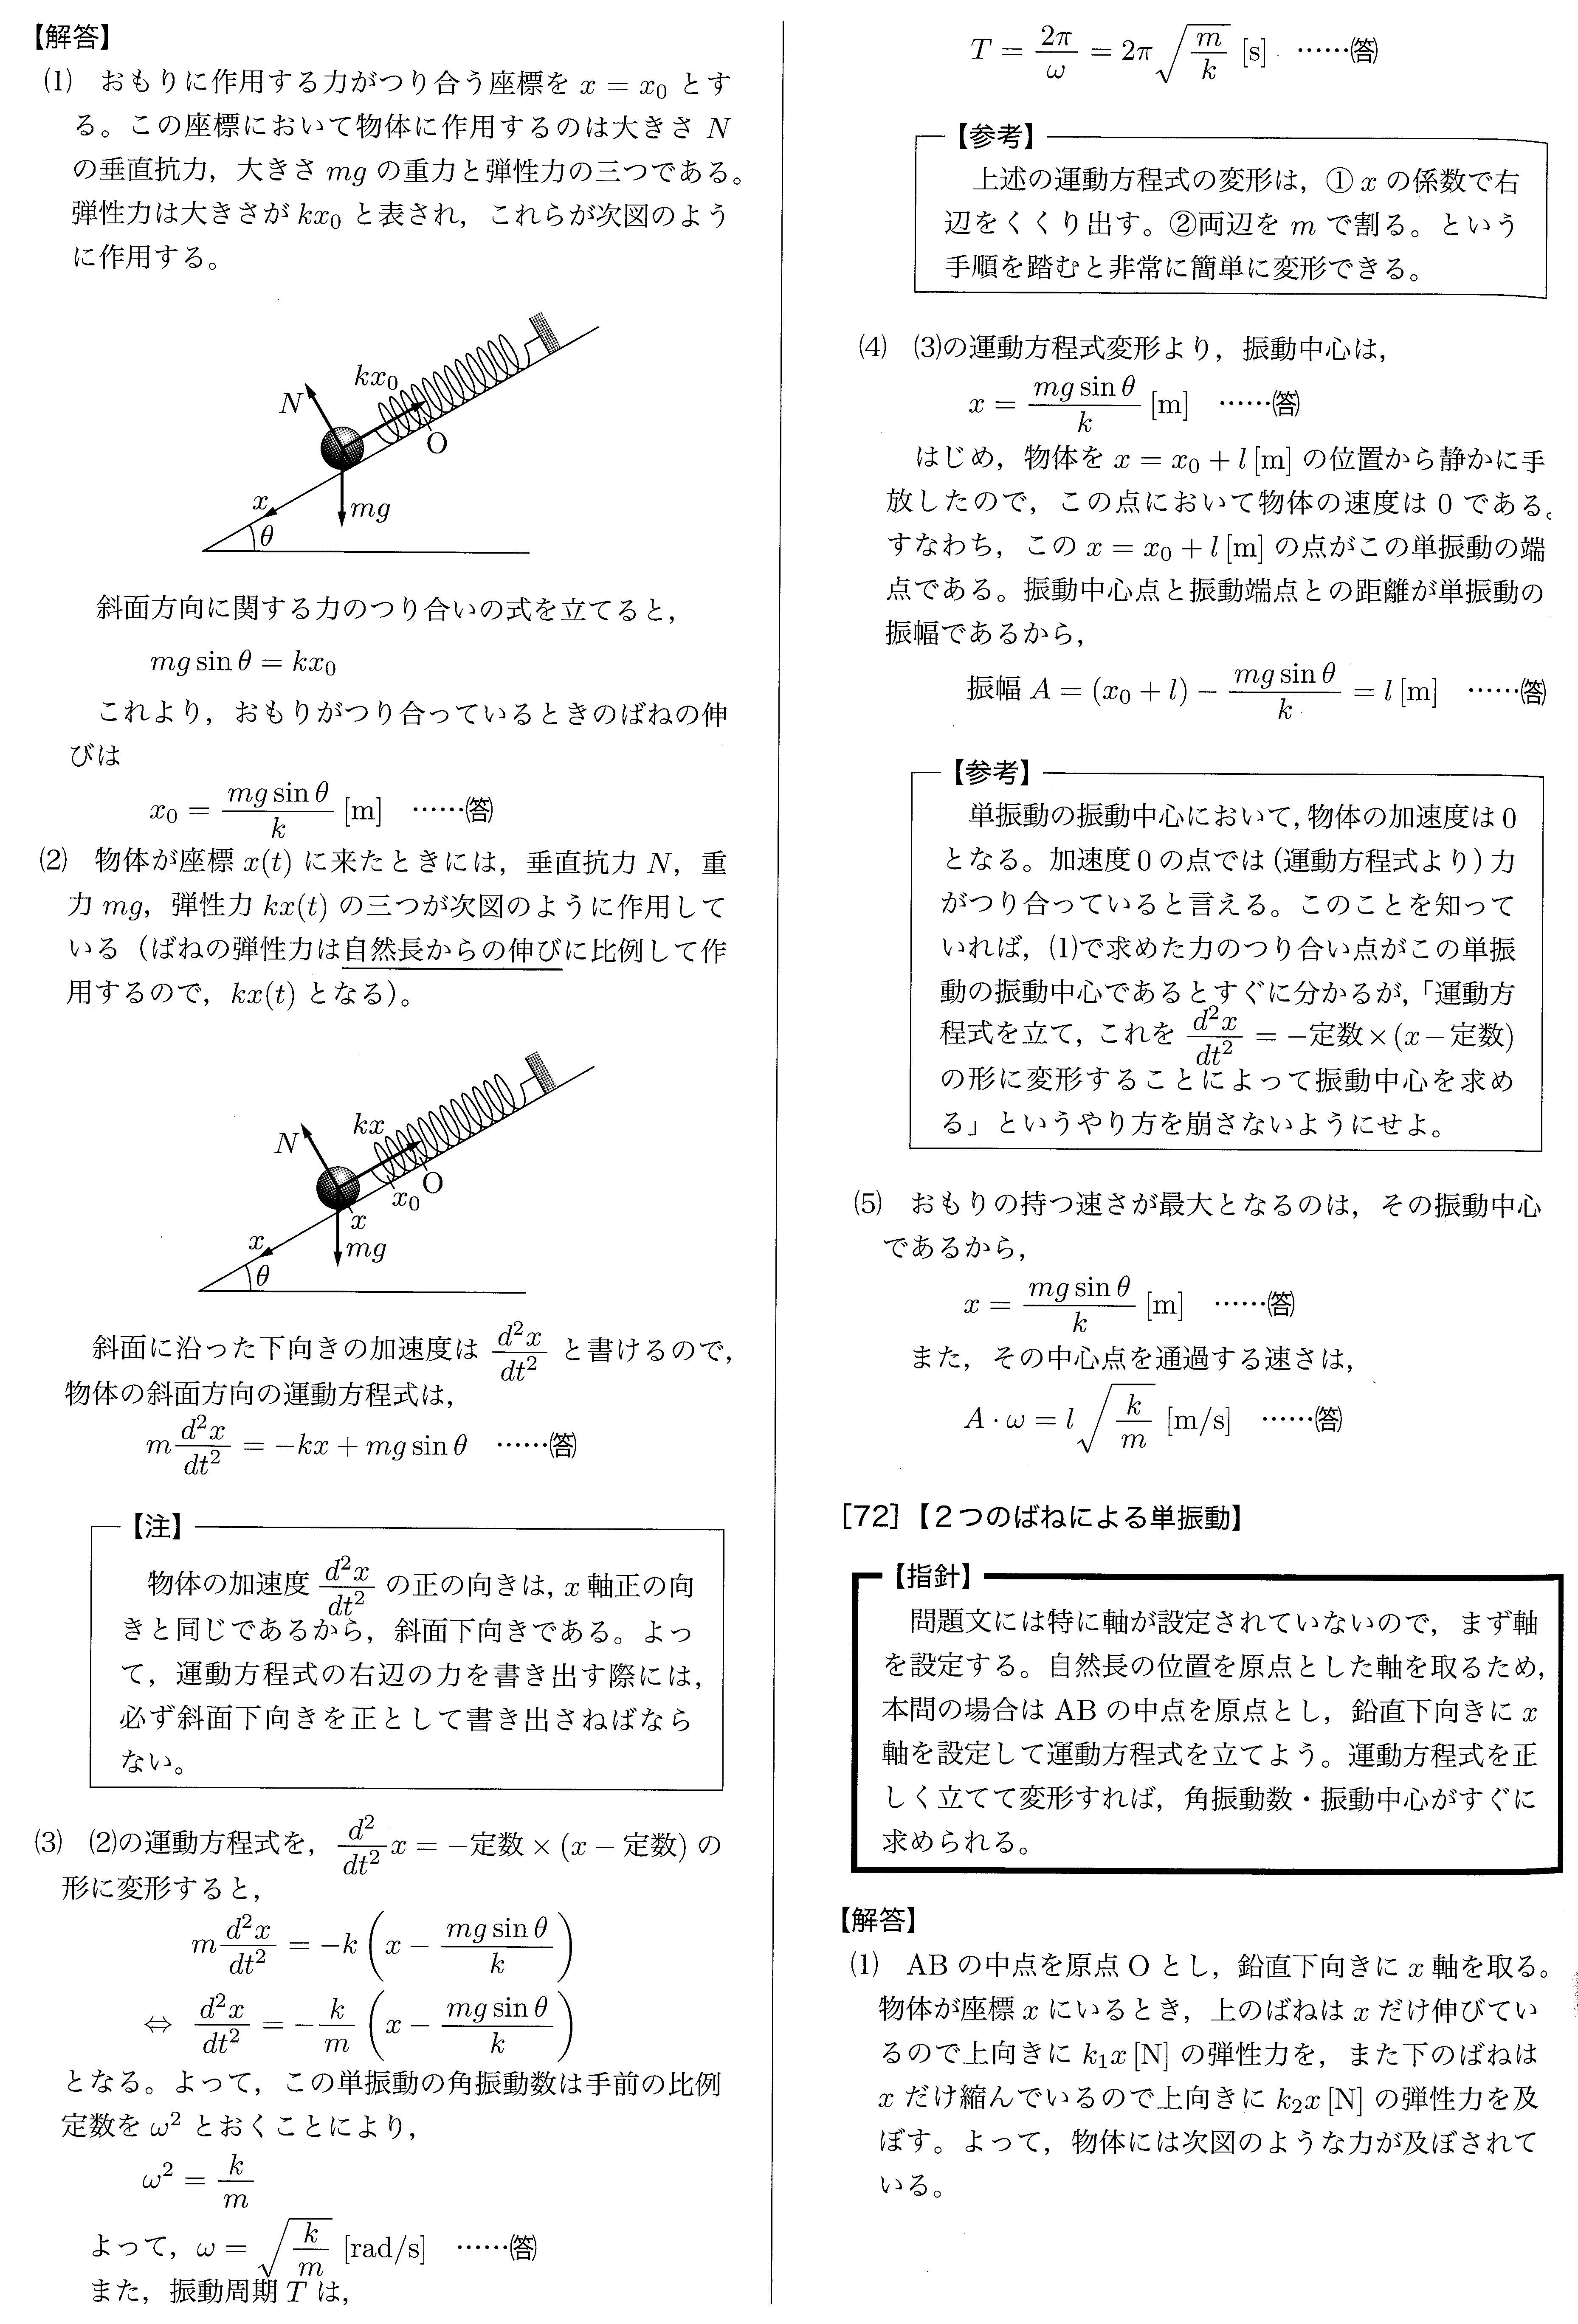
\includegraphics[width=170mm]{prob_p96.png}
\end{center}
\end{figure}
 
 \newpage

\begin{figure}[h]
\begin{center}
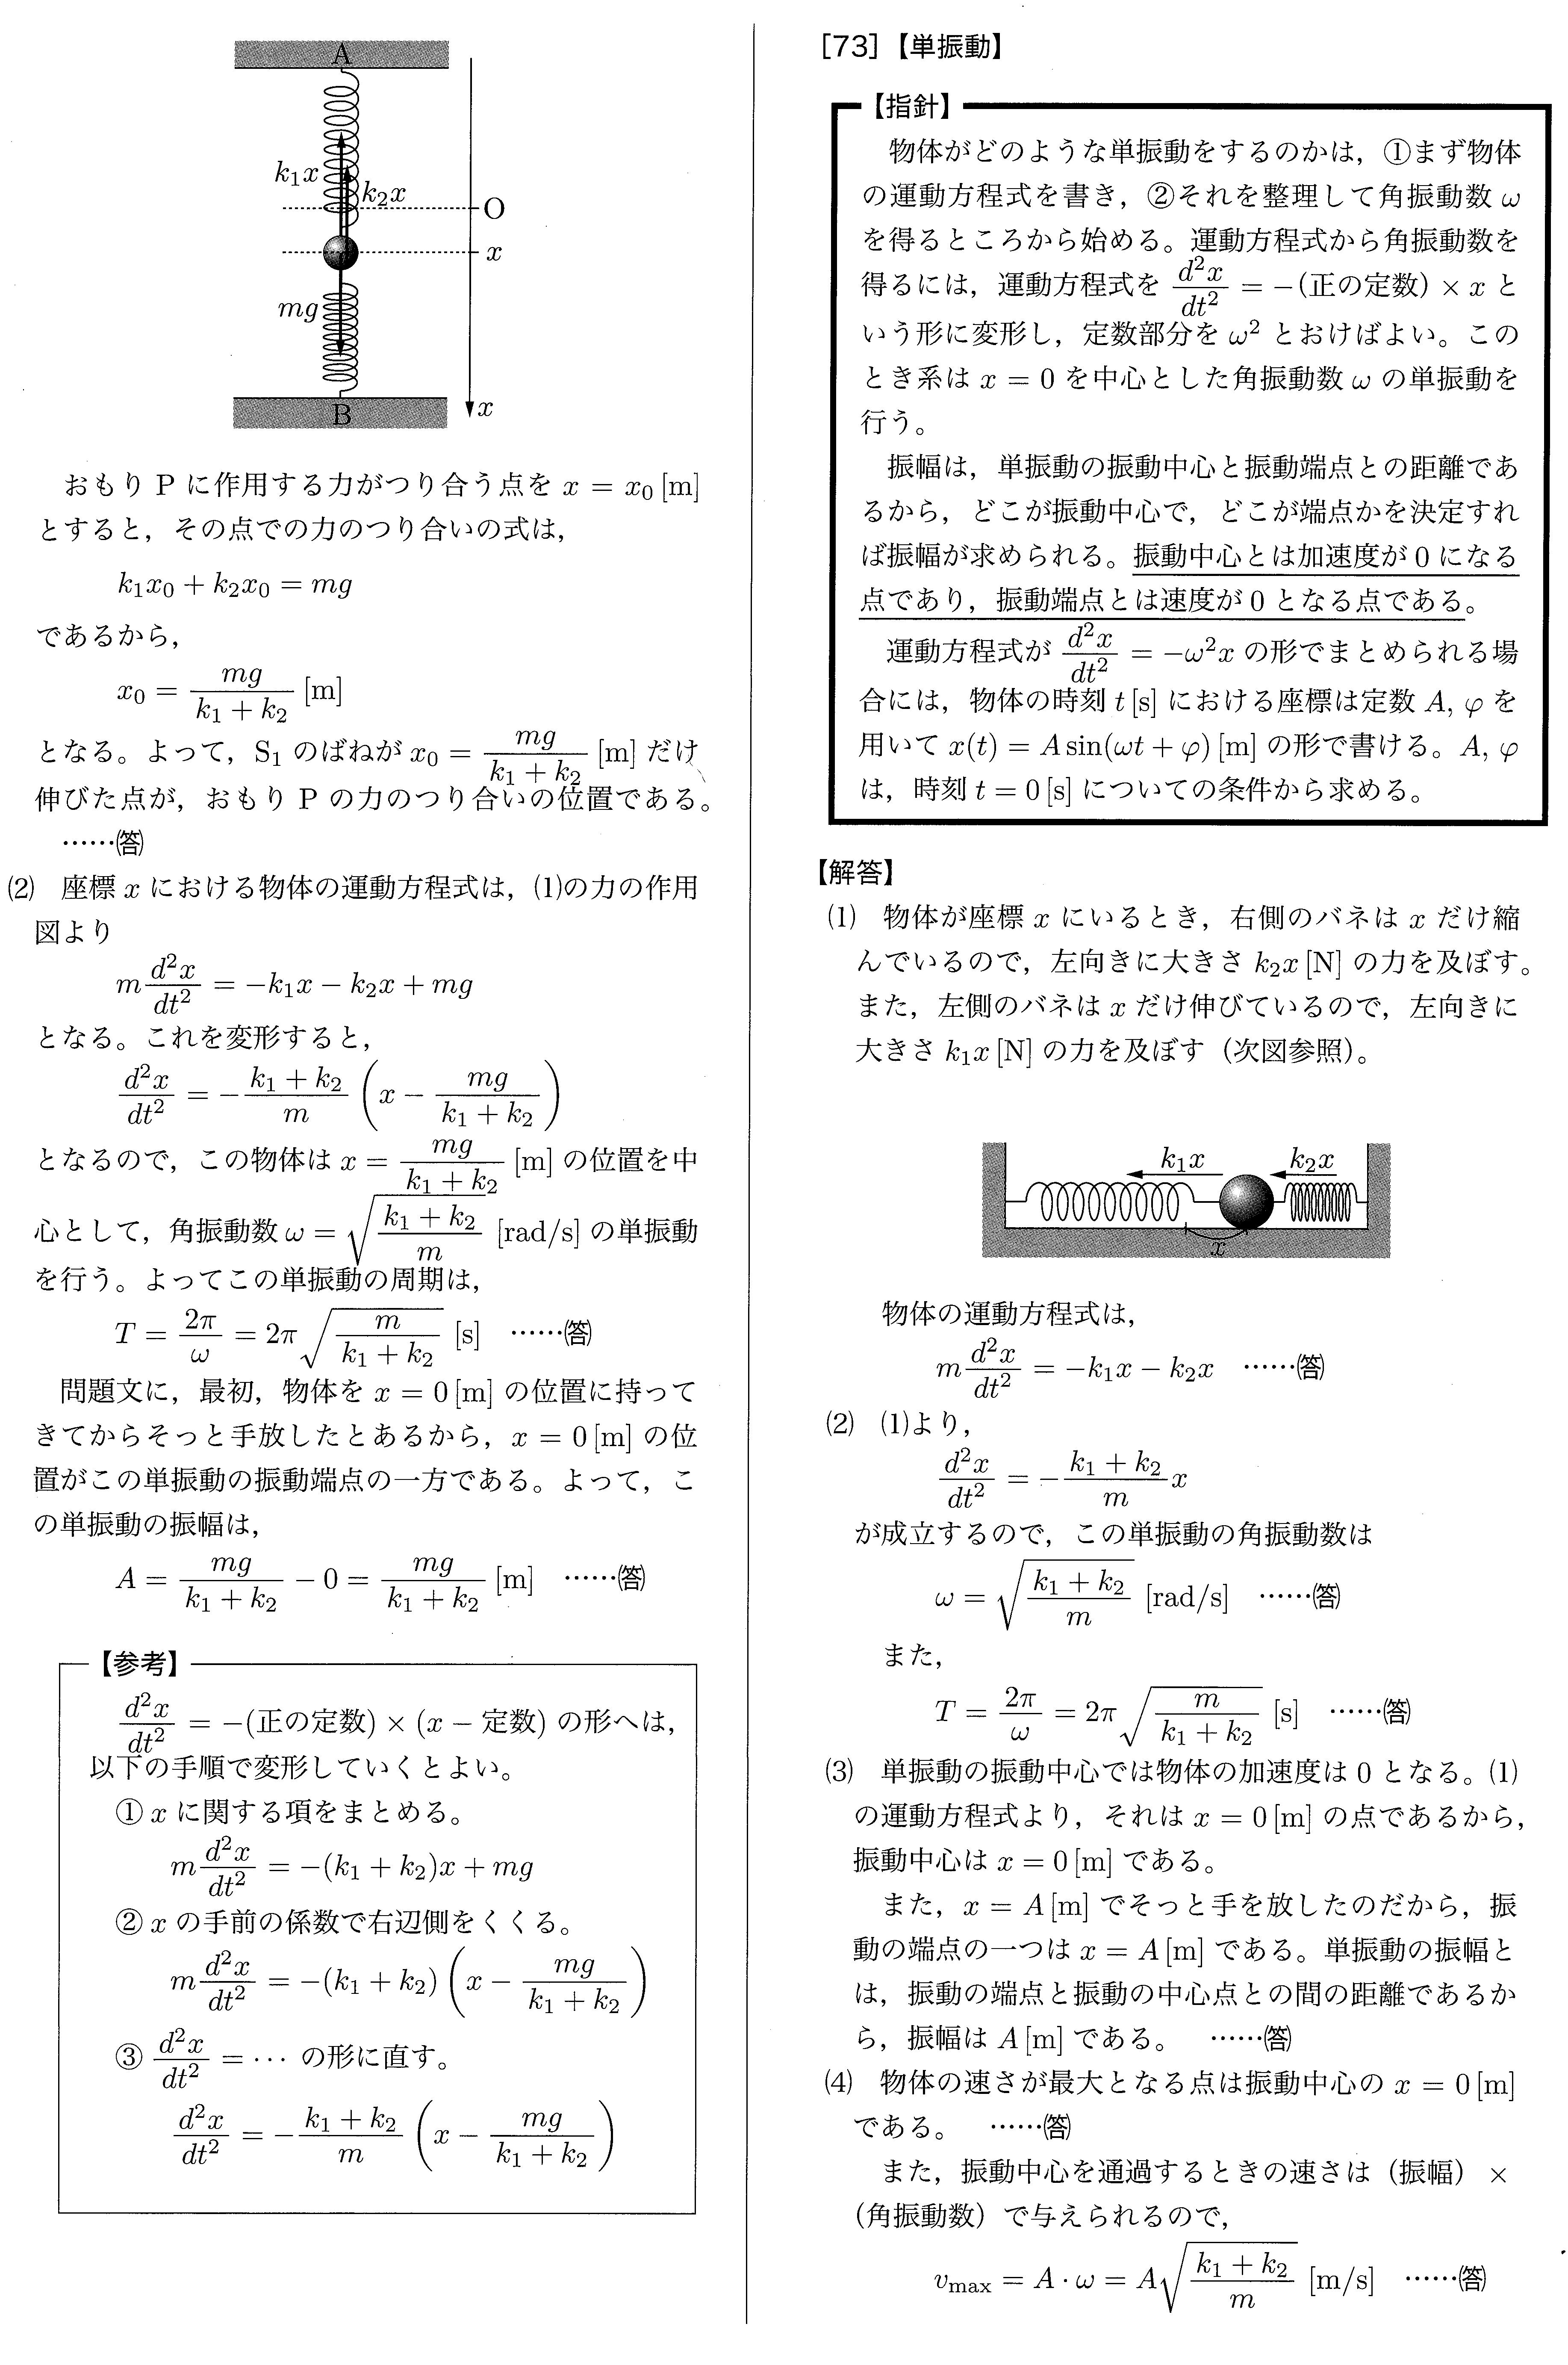
\includegraphics[width=170mm]{prob_p97.png}
\end{center}
\end{figure}

\newpage

\begin{figure}[h]
\begin{center}
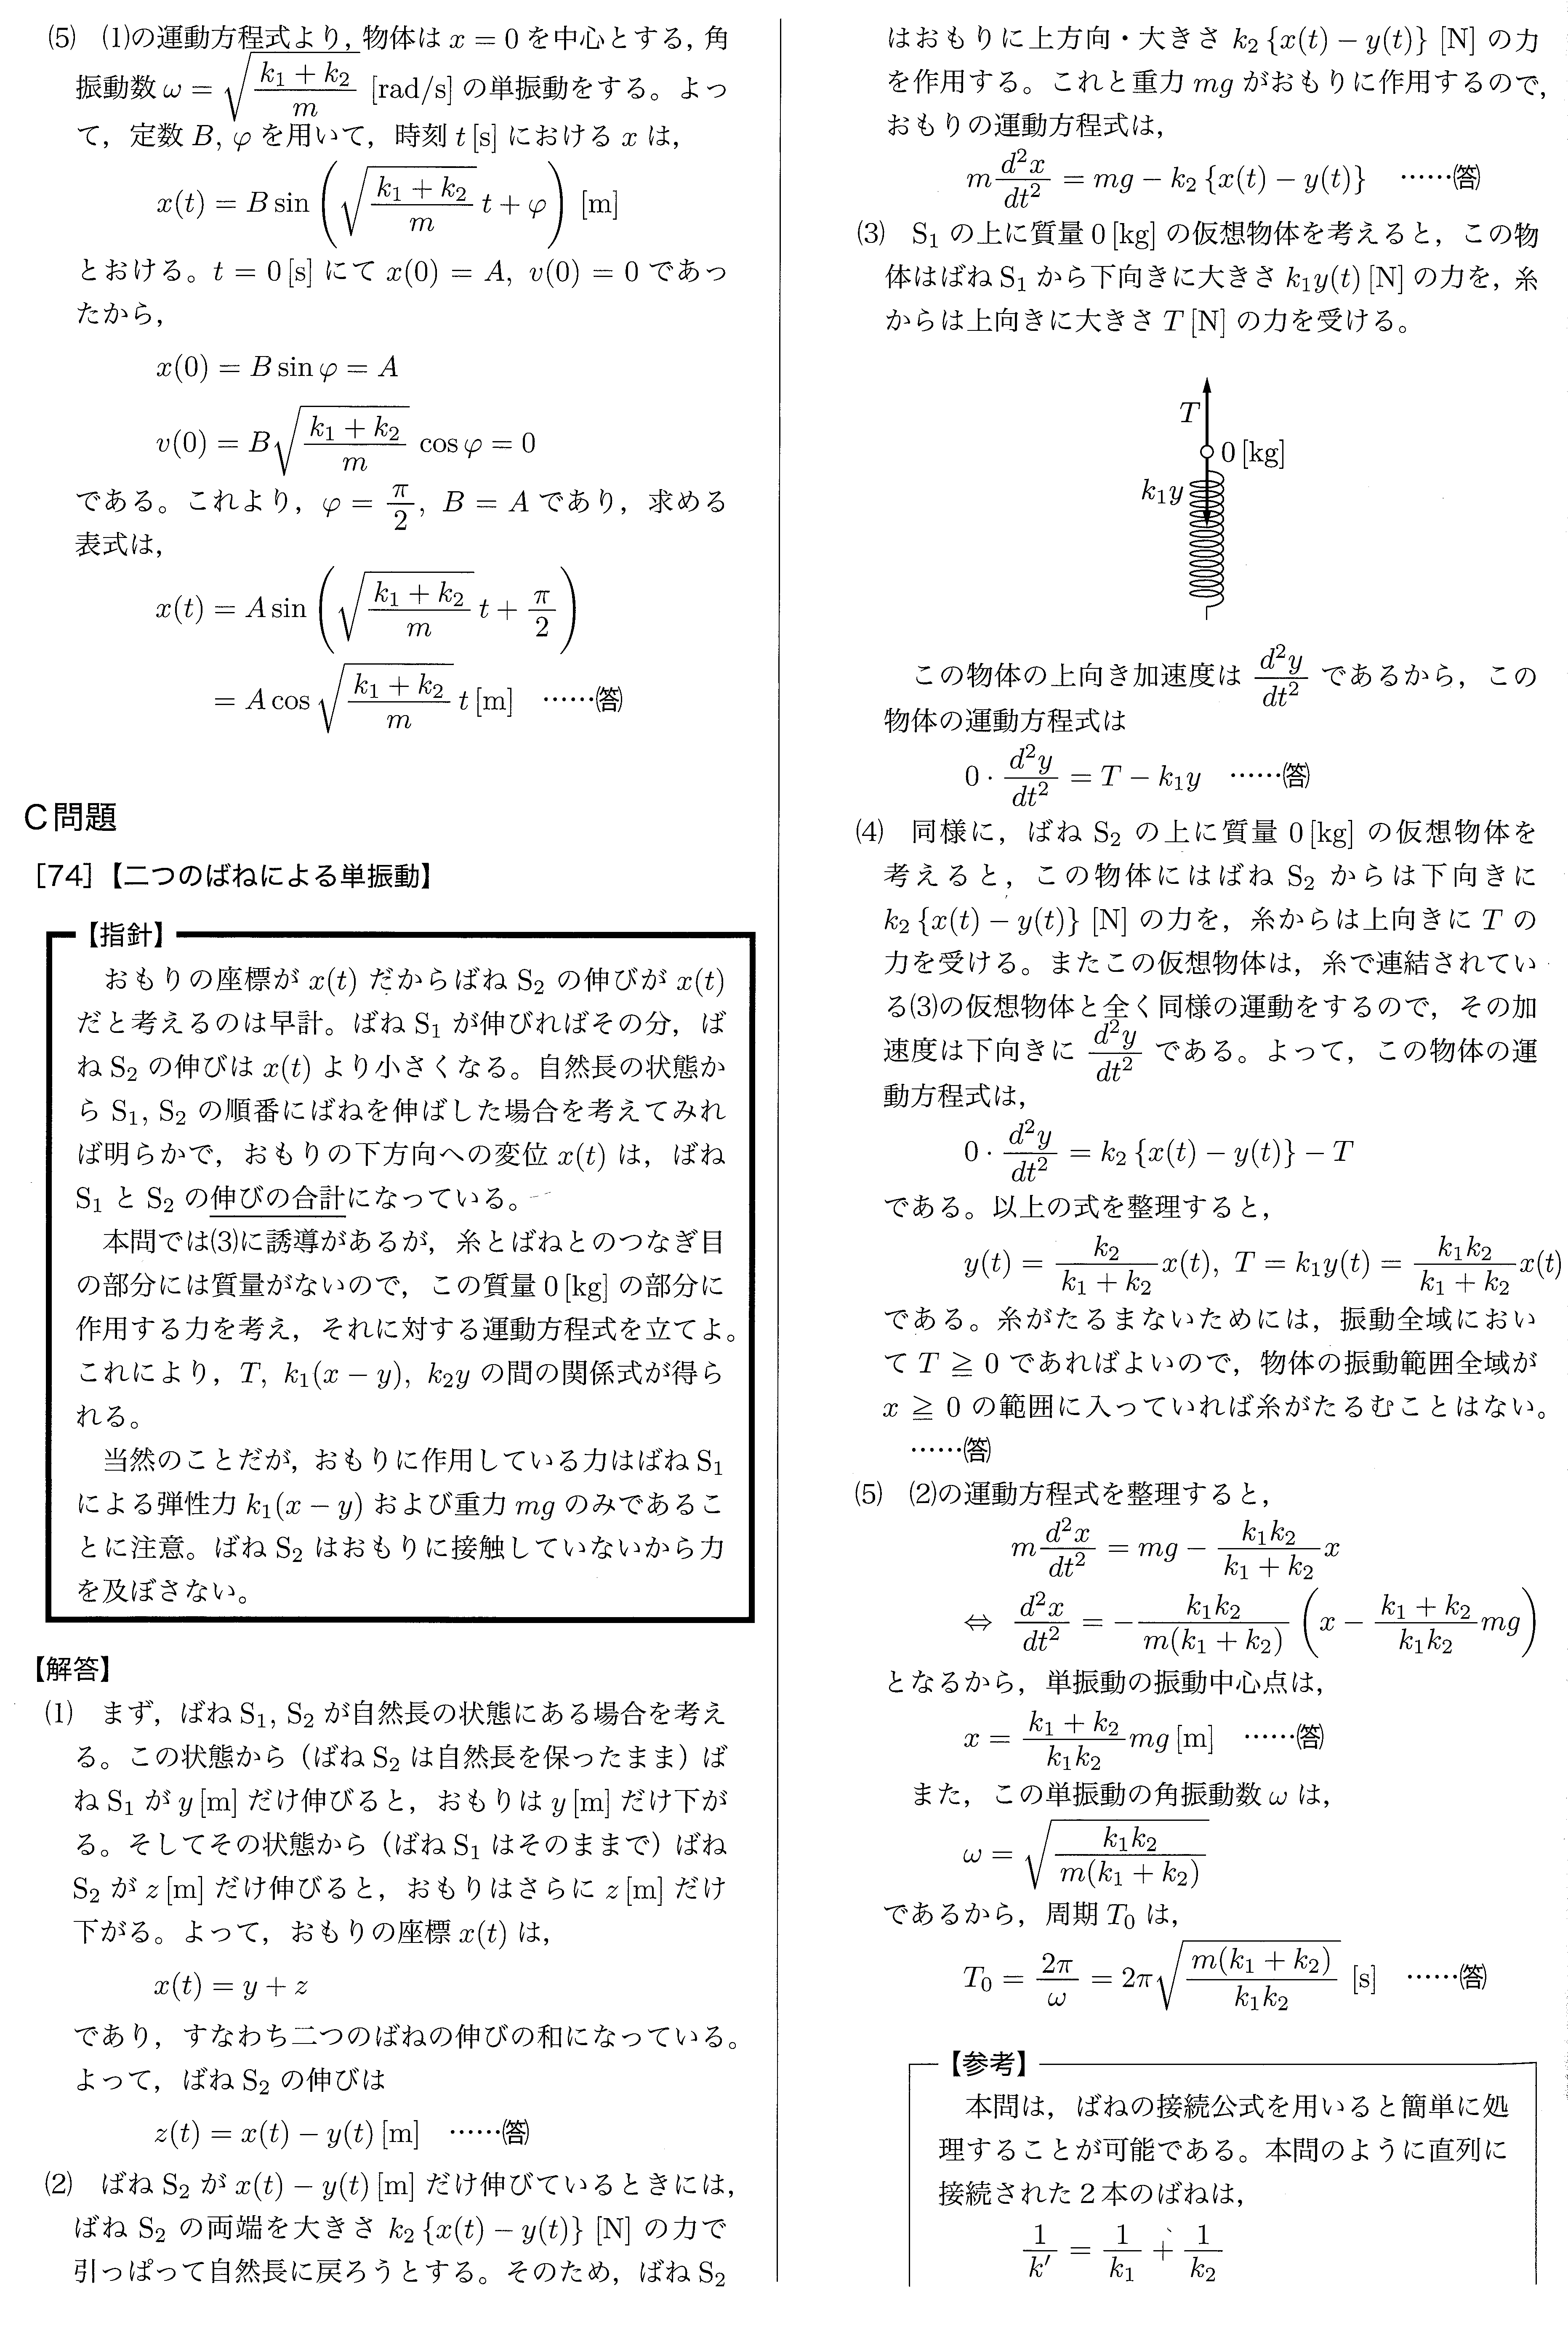
\includegraphics[width=170mm]{prob_p98.png}
\end{center}
\end{figure}

\newpage

\begin{figure}[h]
\begin{center}
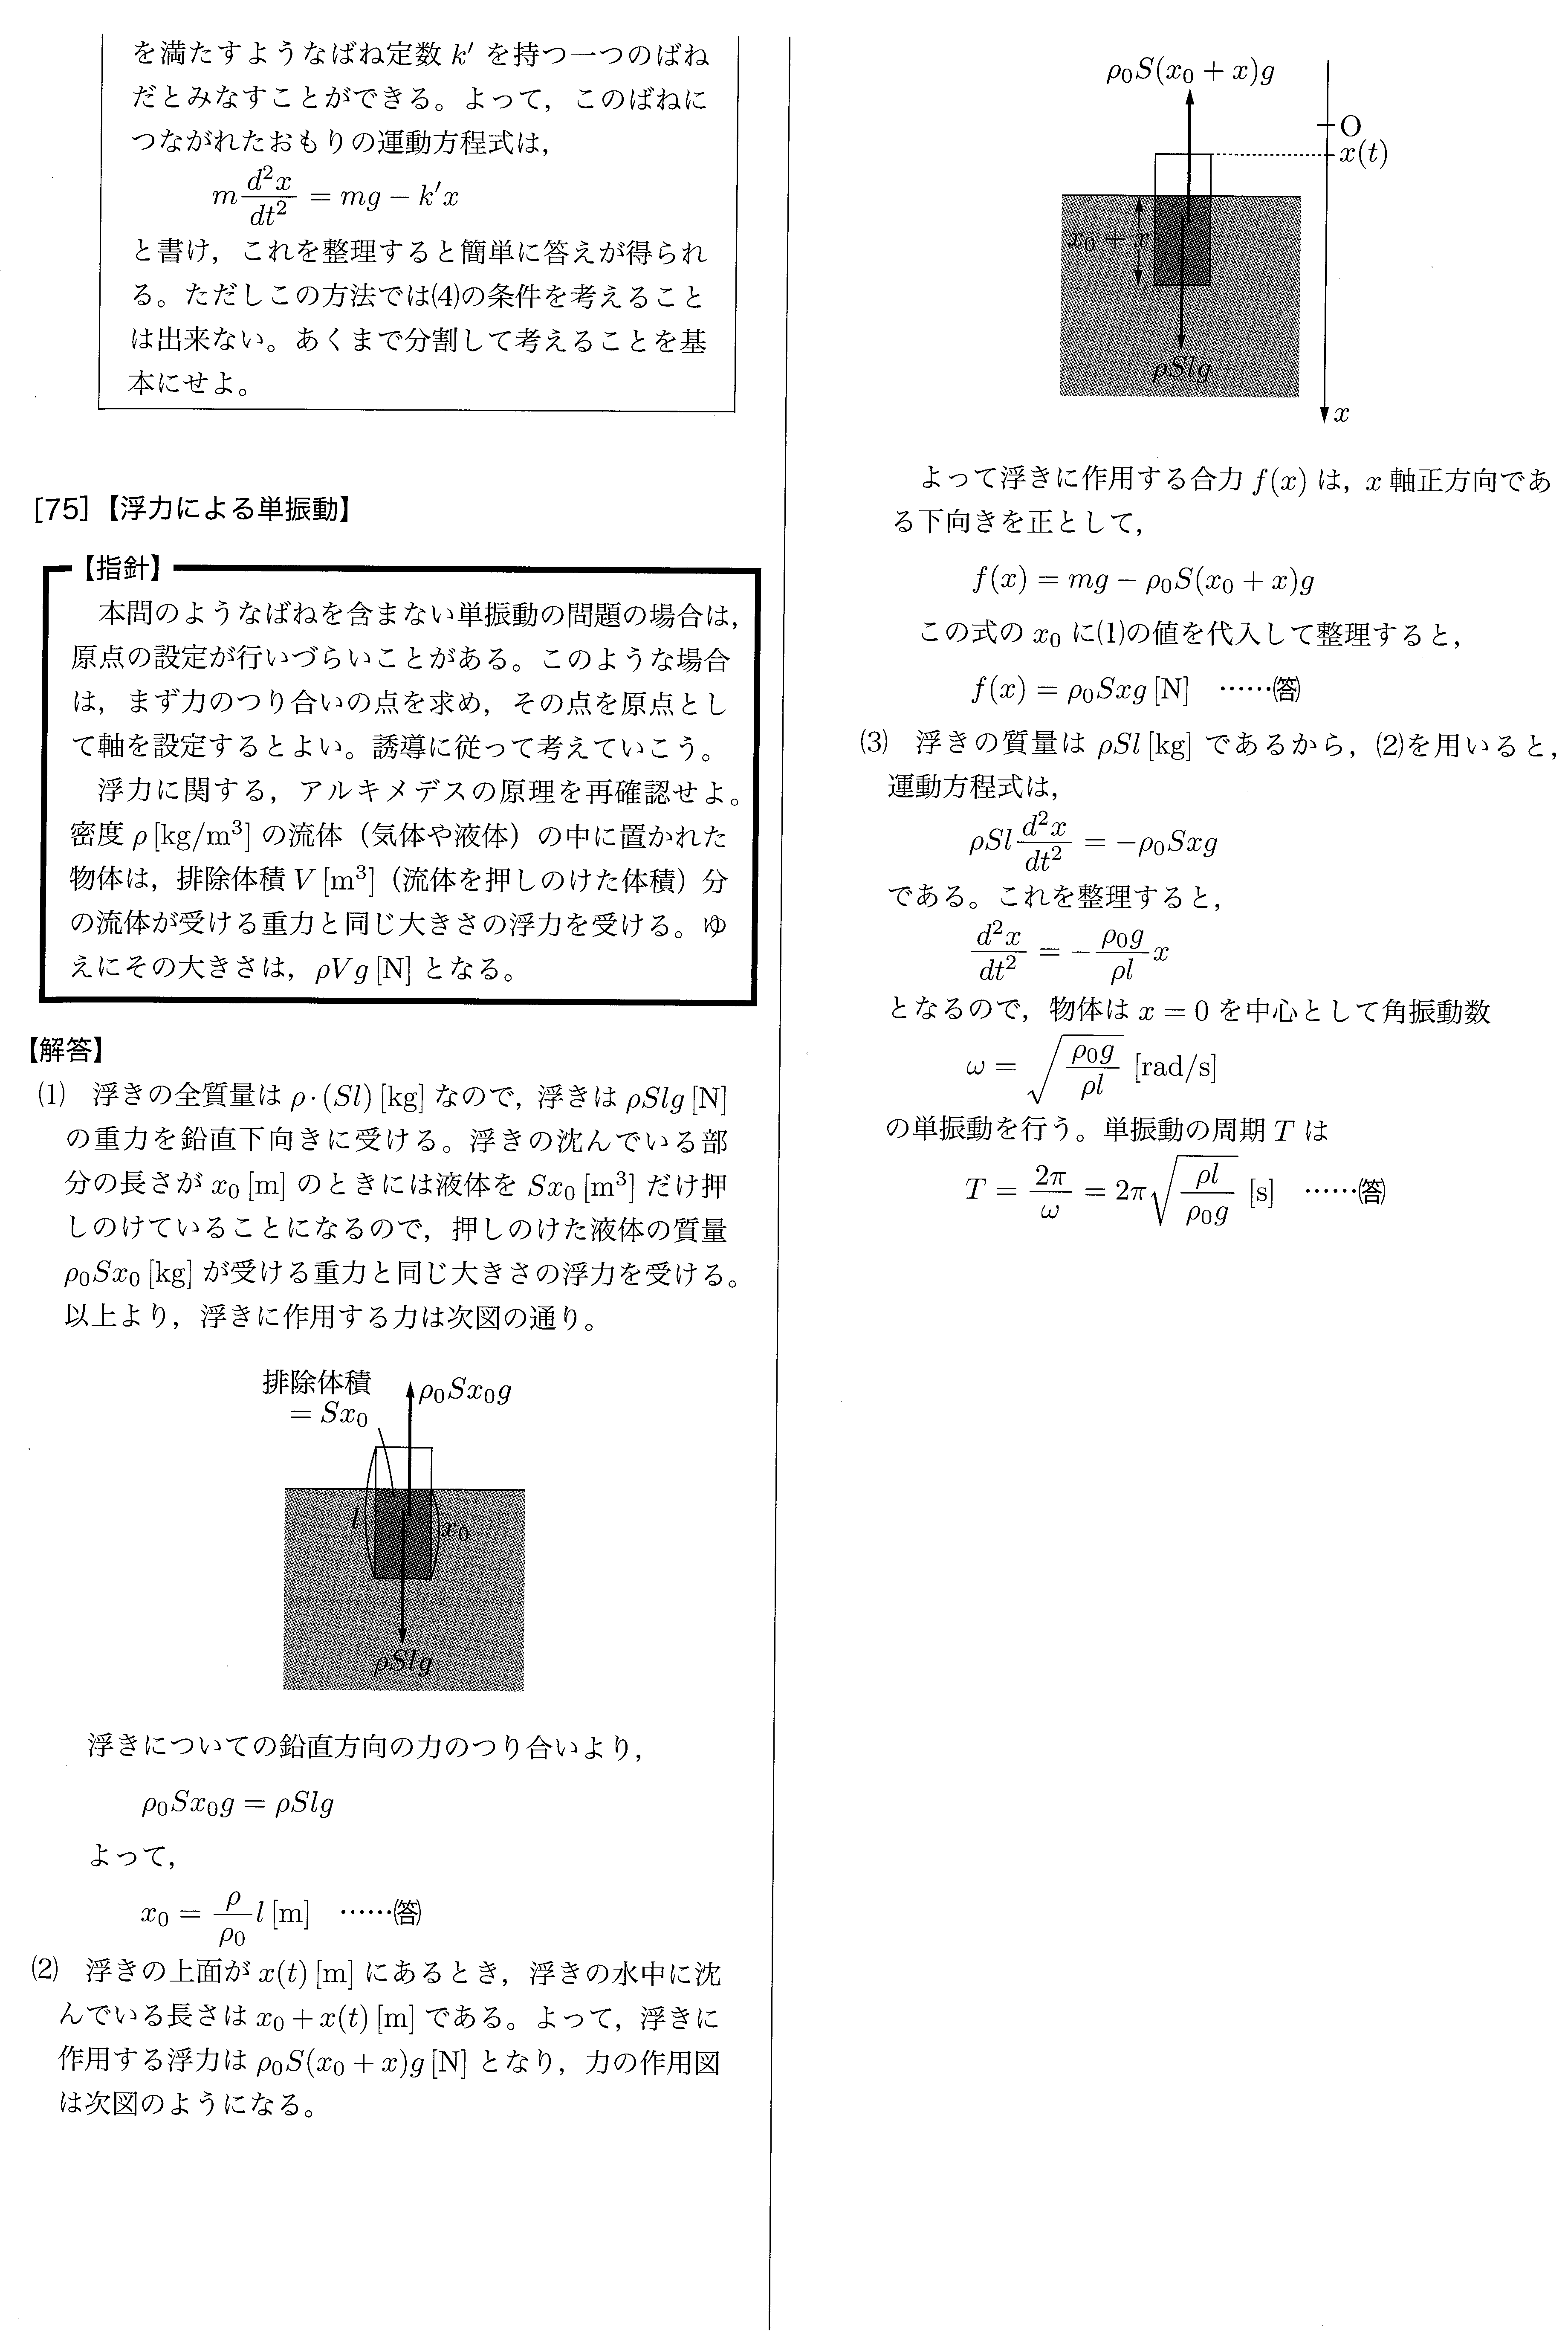
\includegraphics[width=170mm]{prob_p99.png}
\end{center}
\end{figure}
 
 \ 
 
\newpage
\include{physics_ch10}
 \ 
 
\newpage
\section{万有引力・惑星運動（1）}

\subsection{万有引力の法則}

\begin{wrapfigure}[7]{r}[5mm]{50mm}
  \centering
  \vspace{-5mm}
  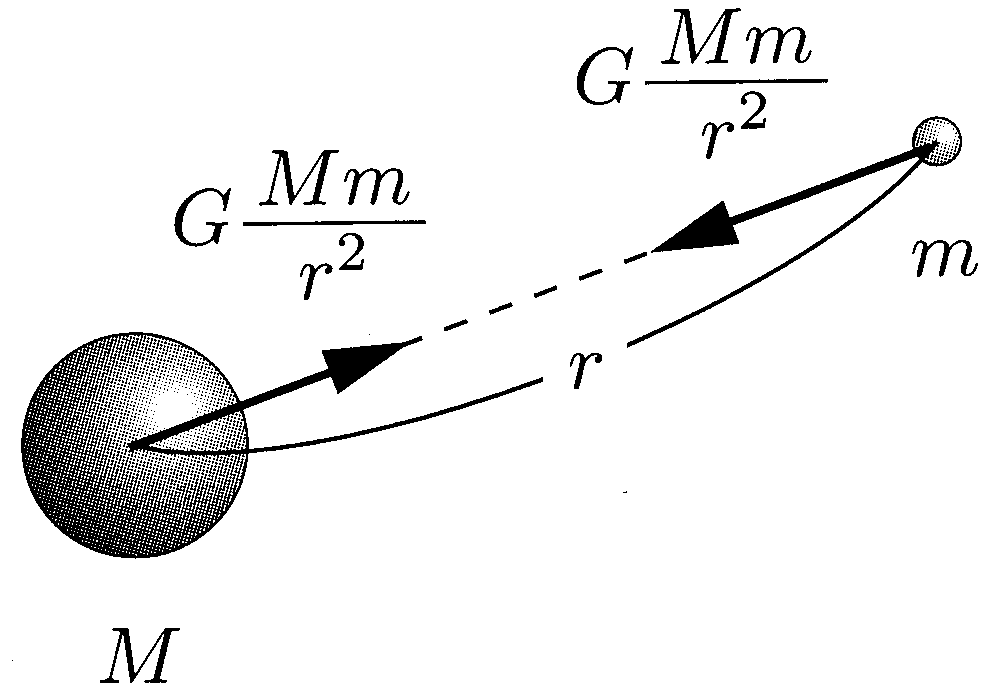
\includegraphics[keepaspectratio,width=40mm]
  {text_p50_fig1.png}
\end{wrapfigure}

質量$M$[kg]の物体Aと質量$m$[kg]の物体Bが距離$r$[m]だけ隔てて置かれている場合について考える．
このとき，この2つの物体はその質量に応じて互いに引力を及ぼし合う．
これを{\bf 万有引力}といい，その大きさ$f$[N]は
\[ f=G\dfrac{Mm}{r^2} {\rm [N]} \]
で与えられる．
向きは{\bf 互いに引き合う向き}で，作用・反作用の法則より各物体に作用する力の大きさは同じである．
比例定数$G{\rm [N・m^2/kg^2]}$を万有引力定数といい，その大きさは実験により$G=6.672\times 10^{-11}{\rm [N・m^2/kg^2]}$であることが知られている．

この万有引力は非常に微小な力であるため，通常の力学問題では重力以外の万有引力は無視してよい．
この万有引力が問題になるのは惑星運動のときが主である．

\begin{matome}{万有引力の法則}

\hspace{3mm}質量$M$[kg]の物体と質量$m$[kg]の物体が距離$r$[m]だけ隔てて置かれているとき，2つの物体間には互いに引き合う方向に，大きさ
 \[ f=G\dfrac{Mm}{r^2} \hspace{2mm}[N]\]
 の万有引力が作用する．（ただし，$G{\rm [N・m^2/kg^2]}$は万有引力定数）
 \end{matome}

 \ 
 
%\begin{breakbox}
%\ex＜万有引力による等速円運動＞\\
%
%地球の周りを等速円運動する物体について以下の問いに答えよ．
%ただし，地球の質量を$M$[kg]，万有引力定数を$G{\rm [N・m^2/kg^2]}$，地球の半径を$R$[m]，地球表面における重力加速度の大きさを$g{\rm [m/s^2]}$，地球の自転周期を$T$[s]とする．
%\begin{description}
%\item[(1)] 地球表面で地球から物体に作用する万有引力が地表における重力であることを利用して，$G$と$g$との間に成り立つ関係を与えられた文字を用いて表せ．
%\item[(2)] (1)をもとに，地表から高度$h$[m]の高さで地球から万有引力による物体の加速度の大きさ$g(h)[{\rm m/s^2}]$を求めよ．
%\item[(3)] 赤道上高度$h$[m]の高さを等速円運動している人工衛星の速さ$V$[m/s]を$G,M,R,h$を用いて表せ．
%\item[(4)] この人工衛星が静止衛星となるにはどれだけの高度の位置を飛行すればよいか．$g,R,T$を用いて表せ．
%\end{description}
%
%\end{breakbox}

%\newpage

\subsection{万有引力による位置エネルギー}

\begin{wrapfigure}[7]{r}[5mm]{80mm}
  \centering
  \vspace{-5mm}
  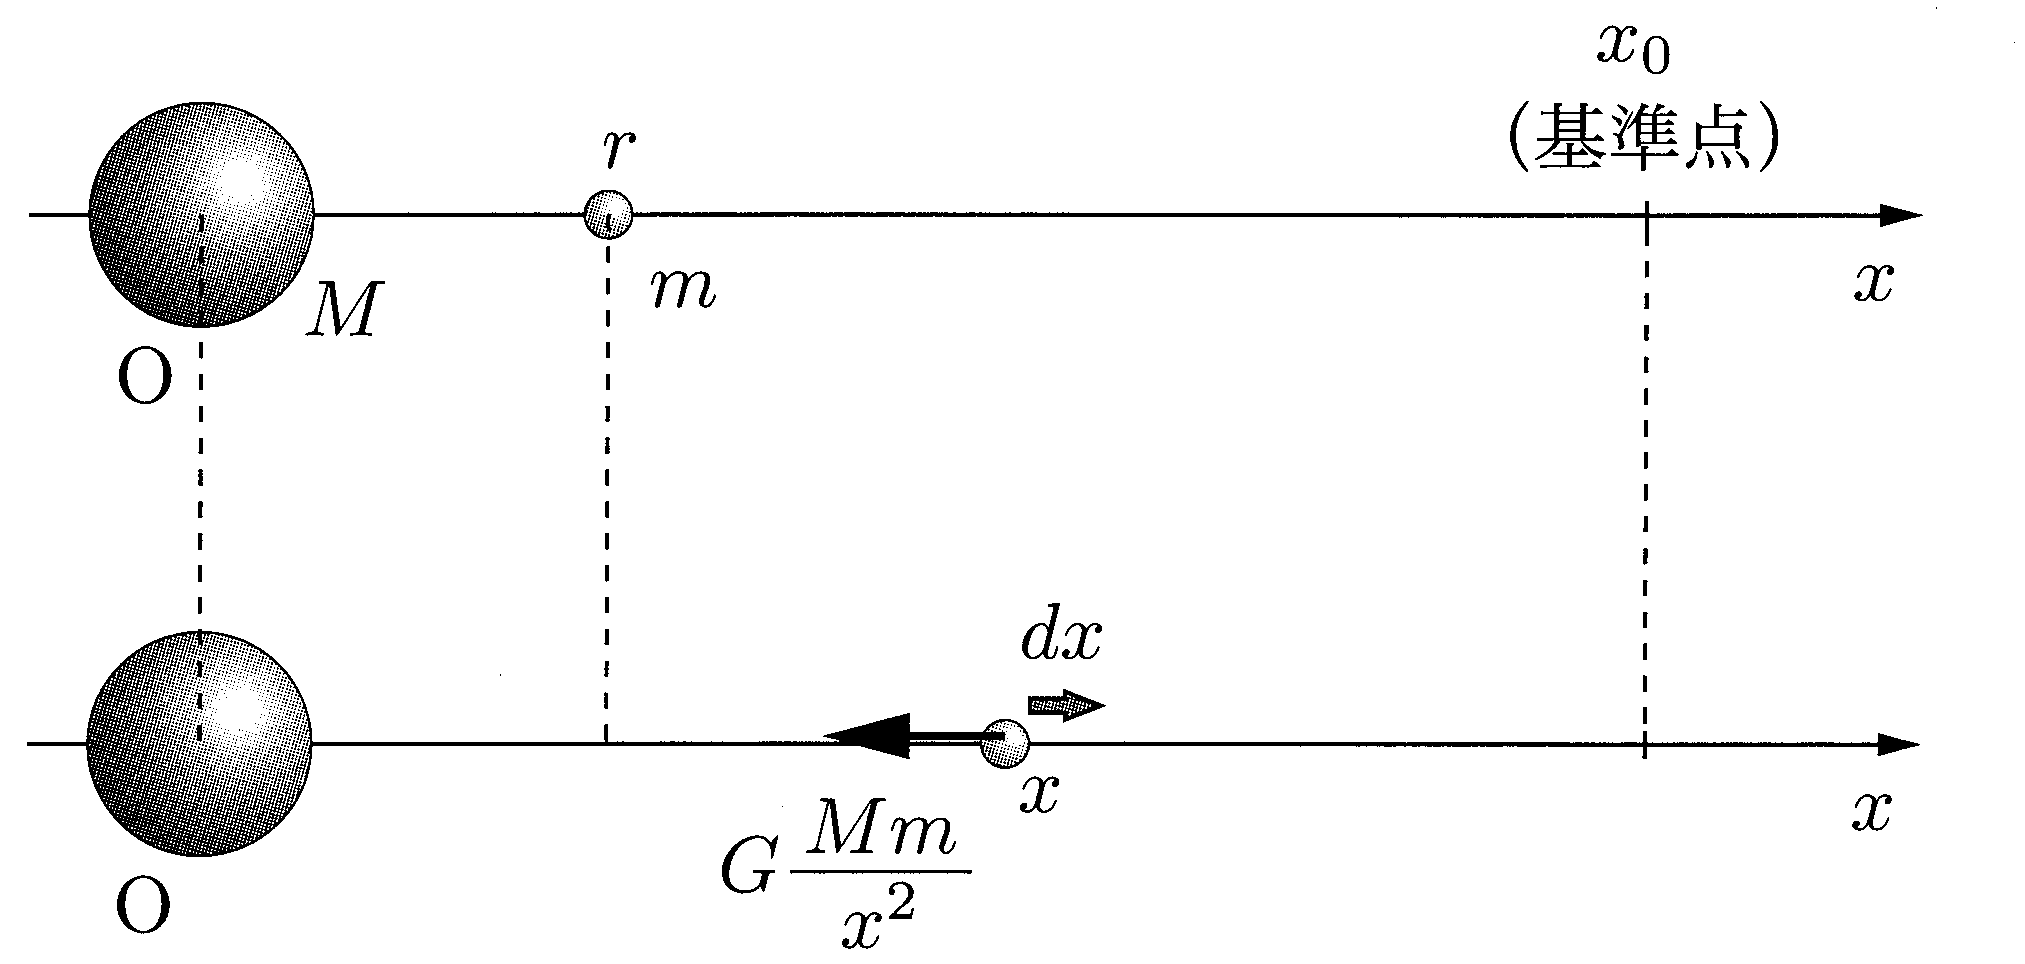
\includegraphics[keepaspectratio,width=80mm]
  {text_p51_fig1.png}
\end{wrapfigure}

重力やバネによる弾性力などと同様に万有引力も保存力であり，万有引力に関する位置エネルギーを考えることができる．
位置エネルギーとは，基準点と比較したときに余分に持っているエネルギーのことであり，その状態から基準点まで移動したときに位置エネルギーの元となる力が物体に対してなす仕事に等しい．
このことを用いて万有引力による位置エネルギーの式を求める．

質量$M$[kg]の物体が図のO点に固定されており，これから距離$r$[m]の位置に質量$m$[kg]の物体があるとする．
図のように$x$軸を設定し，この物体を基準点$x_0$[m]の位置まで動かすときに万有引力のする仕事を計算する．
物体に作用する万有引力は位置によって大きさが変化するので，微小区間に分けて考える．
物体が位置$x$[m]から$x+dx$[m]まで動くときに万有引力がする微小な仕事$dW$[J]は，
\[ dW=-G\dfrac{Mm}{x^2} ・dx\hspace{2mm}{\rm [J]}\]
で与えられる．
位置$x=r$[m]から基準点$x=x_0$[m]まで動くときに万有引力のする仕事の総和は
\[ W=\int^{x=x_0}_{x=r}dW=\int^{x=x_0}_{x=r}\left( -G\dfrac{Mm}{x^2}\right) dx=G\dfrac{Mm}{x_0}-G\dfrac{Mm}{r}\hspace{2mm}[J]\]
と計算される．
ゆえに質量$m$[kg]の物体が位置$x=r$[m]で持つ位置エネルギーは
\[ U=G\dfrac{Mm}{x_0}-G\dfrac{Mm}{r} \hspace{2mm}{\rm [J]}\]
で与えられる．

\begin{wrapfigure}[7]{r}[5mm]{60mm}
  \centering
  \vspace{-5mm}
  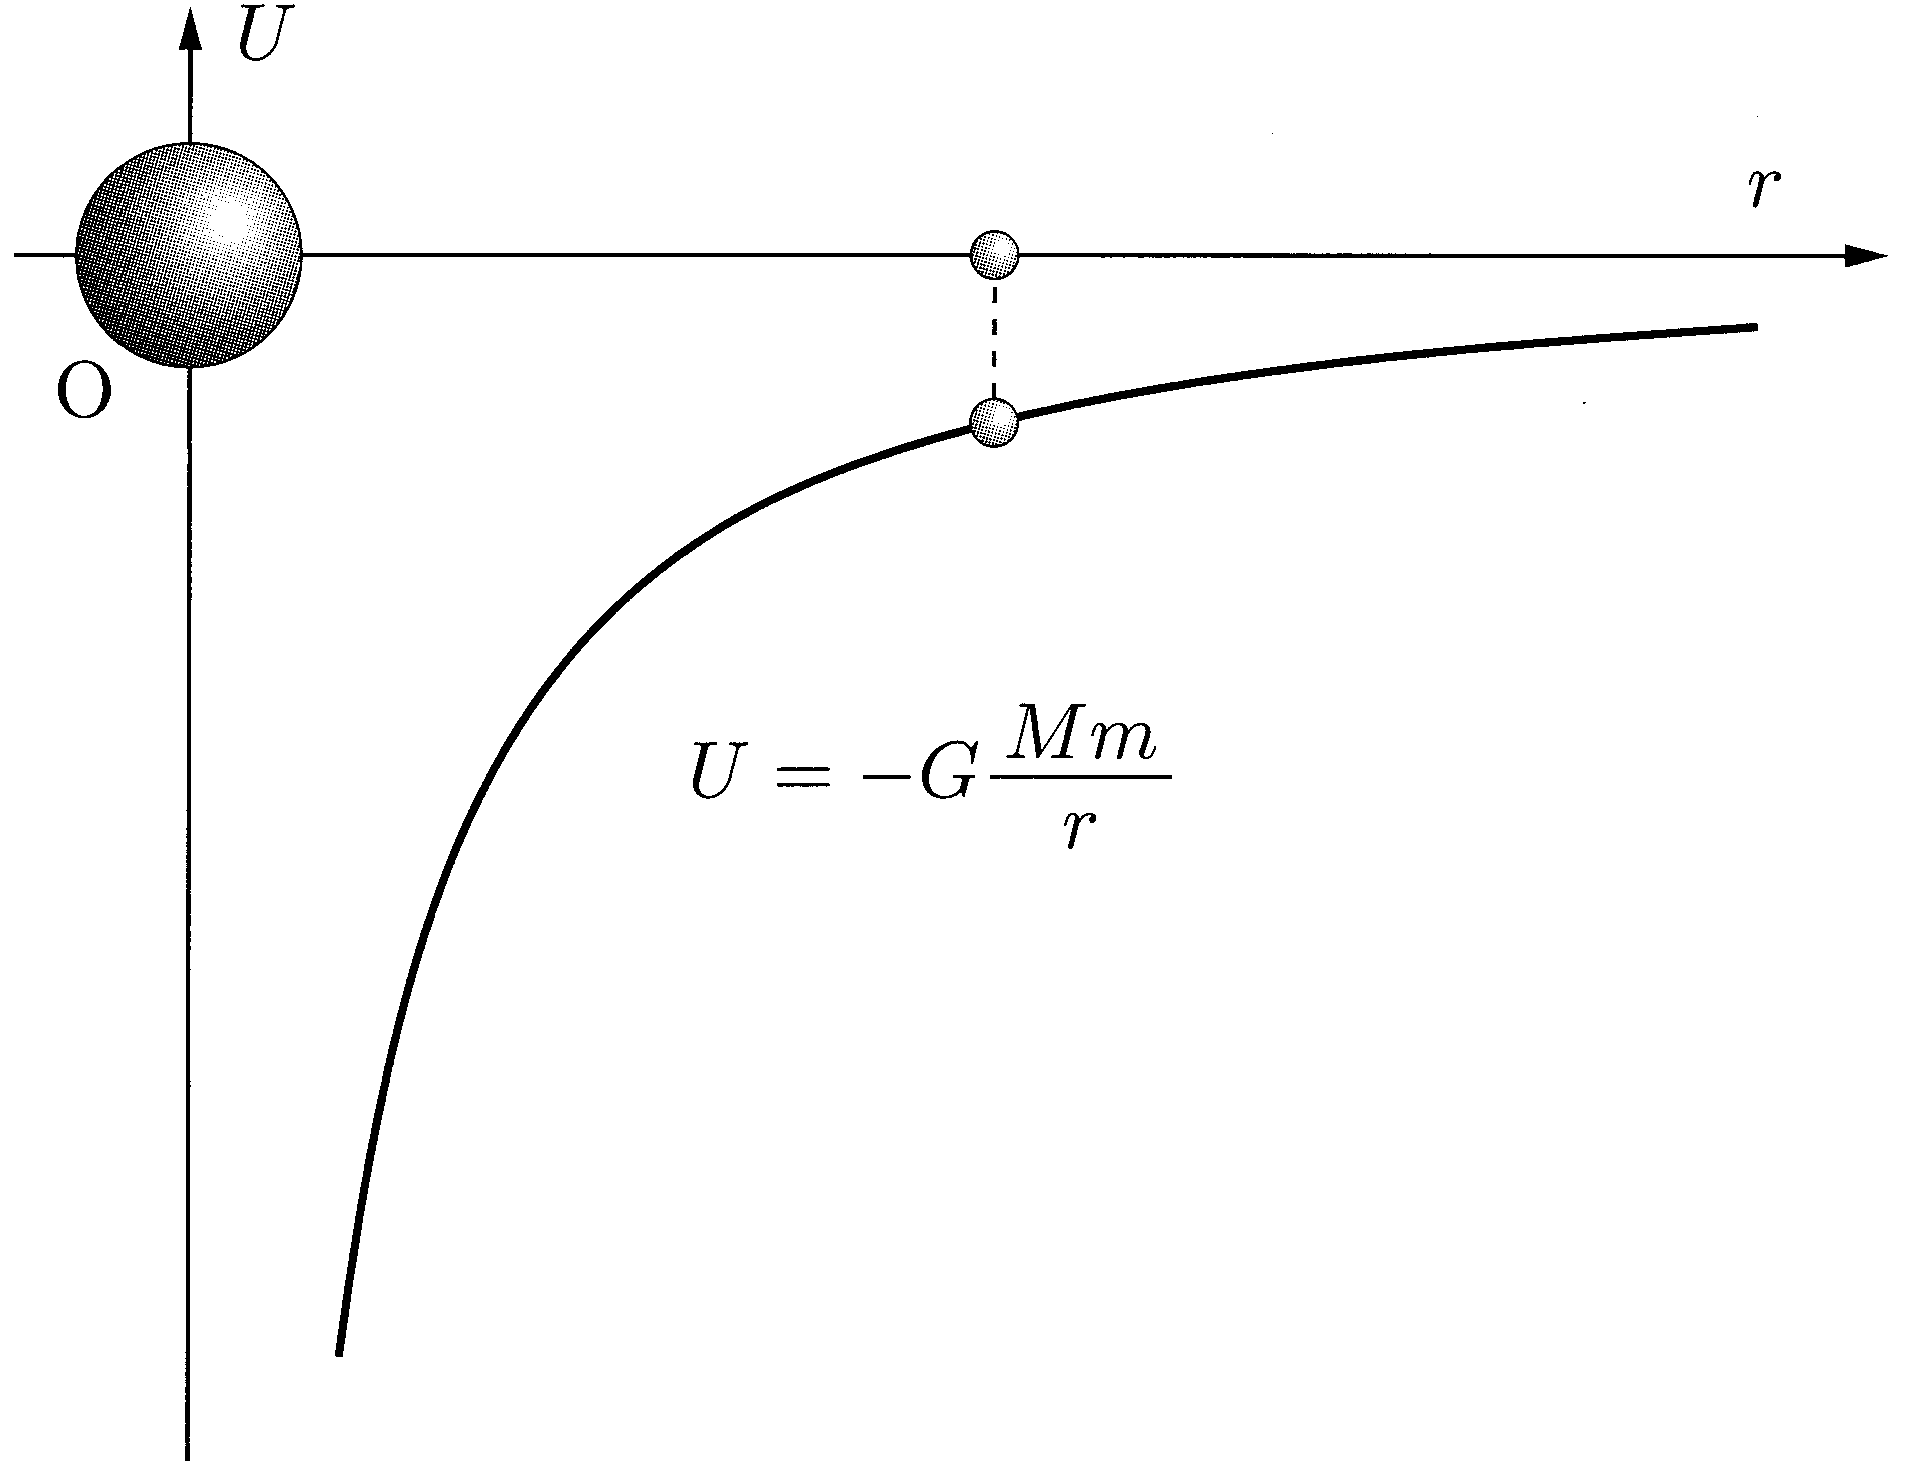
\includegraphics[keepaspectratio,width=50mm]
  {text_p51_fig2.png}
\end{wrapfigure}

さて一般に，位置エネルギーの基準点$x_0$の取り方は任意であるが，上の式において$x_0 \rightarrow \infty$（無限遠点）を基準とすると式の扱いが容易になる．
そこで{\bf 無限遠点を基準点（}\mbox{\boldmath $U=0$} {\bf となる点）}として，質量$m$[kg]の物体が位置$r$[m]で持つ位置エネルギーは
\[ U=-G\dfrac{Mm}{r} \hspace{2mm}[{\rm J}] \]
で与えられる．


\begin{matome}{万有引力による位置エネルギー}

\hspace{3mm}質量$M$[kg]の物体に中心から距離$r$[m]の位置にある質量$m$[kg]の物体の持つ位置エネルギーは，無限遠点を基準として
 \[ U=-G\dfrac{Mm}{r} \hspace{2mm}[J]\]
 で与えられる．
 \end{matome}

 \ 

一般に，万有引力のみによる運動では力学的エネルギー，すなわち物体の運動エネルギーと位置エネルギーの総和が一定に保たれる．
\[ E=\dfrac{1}{2}mv^2-G\dfrac{Mm}{r}=（一定）\]


 \ 
 
%\begin{breakbox}
%\ex＜万有引力による位置エネルギー＞\\
%\begin{wrapfigure}[5]{r}[5mm]{70mm}
%  \centering
%  \vspace{-5mm}
%  \includegraphics[keepaspectratio,width=60mm]
%  {text_p52_fig1.png}
%\end{wrapfigure}
%\hspace{5mm}地球表面から図のように地球の動径方向に質量$m$[kg]のロケットを初速$v_0$[m/s]で打ち上げる場合を考える．
%地球の質量を$M$[kg]，万有引力定数を$G{\rm [N・m^2/kg^2]}$，地球の半径を$R$[m]として以下の問いに答えよ．なお，地球の自転は考えなくてよい．
%\begin{description}
%\item[(1)] このロケットが地球中心から距離$r$[m]の位置にきたときに持つ速さを$v$[m/s]とする．この瞬間と打ち上げた直後との間の力学的エネルギー保存則の式を示せ．
%\item[(2)] (1)をもとに，ロケットが再び地球に戻ってこないために必要な初速度（第二宇宙速度）の大きさを求めよ
%\end{description}
%
%\end{breakbox}

\subsection{ケプラーの法則}

地球は太陽から受ける万有引力により，太陽のまわりを等速円運動している．
しかし詳しい解析によって実際には地球の軌道は完全な円ではなく，楕円軌道であることがわかっている．17世紀の初めにケプラーはチコ・ブラーエの集めた天体運動のデータをもとに，惑星運動に関する以下の3つの法則を発見した．

\begin{matome}{ケプラーの法則}

\hspace{3mm}{\bf 第一法則　楕円軌道の法則}

\hspace{5mm}太陽系の惑星は太陽を1つの焦点とする楕円上を運動する．

\hspace{3mm}{\bf 第二法則　面積速度保存則}

\hspace{5mm}惑星と太陽を結ぶ線分が単位時間あたりに掃く面積は軌道上のすべての点で一定である．
%\[\dfrac{1}{2}rv\sin \theta =（一定）\]

\hspace{3mm}{\bf 第三法則　公転周期と長半径の関係}

\hspace{5mm}惑星の公転周期の2乗は楕円軌道の長半径の3乗に比例する．
\[\dfrac{T^2}{a^3}=（一定）\]
 \end{matome}

 \ 
 
% 
% まずは第三法則について考える．
% 
%  \ 
 
%\begin{breakbox}
%\ex＜ケプラーの第三法則＞\\
%
%ケプラーの第三法則に関する以下の問いに答えよ．
%ただし，太陽の質量を$M_s$[kg]，万有引力定数を$G{\rm [N・m^2/kg^2]}$とする．
%\begin{description}
%\item[(1)] 太陽から距離$r$[m]の半径で等速円運動する質量$m$[kg]の惑星について，その公転周期$T$[s]と半径$r$[m]について$\dfrac{T^2}{a^3}$の比の値が惑星自身の質量$m$[kg]に依存しないことを示せ．
%\item[(2)] ハレー彗星は1986年2月に太陽に最接近している．このハレー彗星は周期76年で，近日点距離（太陽との最接近距離）は0.59天文単位である．ハレー彗星の遠日点距離はおよそ何天文単位か．ただし，1天文単位は$1.5\times 10^{11}$[m]で，これは太陽と地球との距離である．
%\item[(3)] ハレー彗星の遠日点は相当に遠いので，無限遠点から初速度0[m/s]で太陽に近づいてくると近似して，近日点でのハレー彗星の速さを求めよ．ただし，$GM_s=1.3\times 10^{20}[{\rm m^3/s^2}]$
%\end{description}
%
%\end{breakbox}

  \newpage

\begin{figure}[h]
\begin{center}
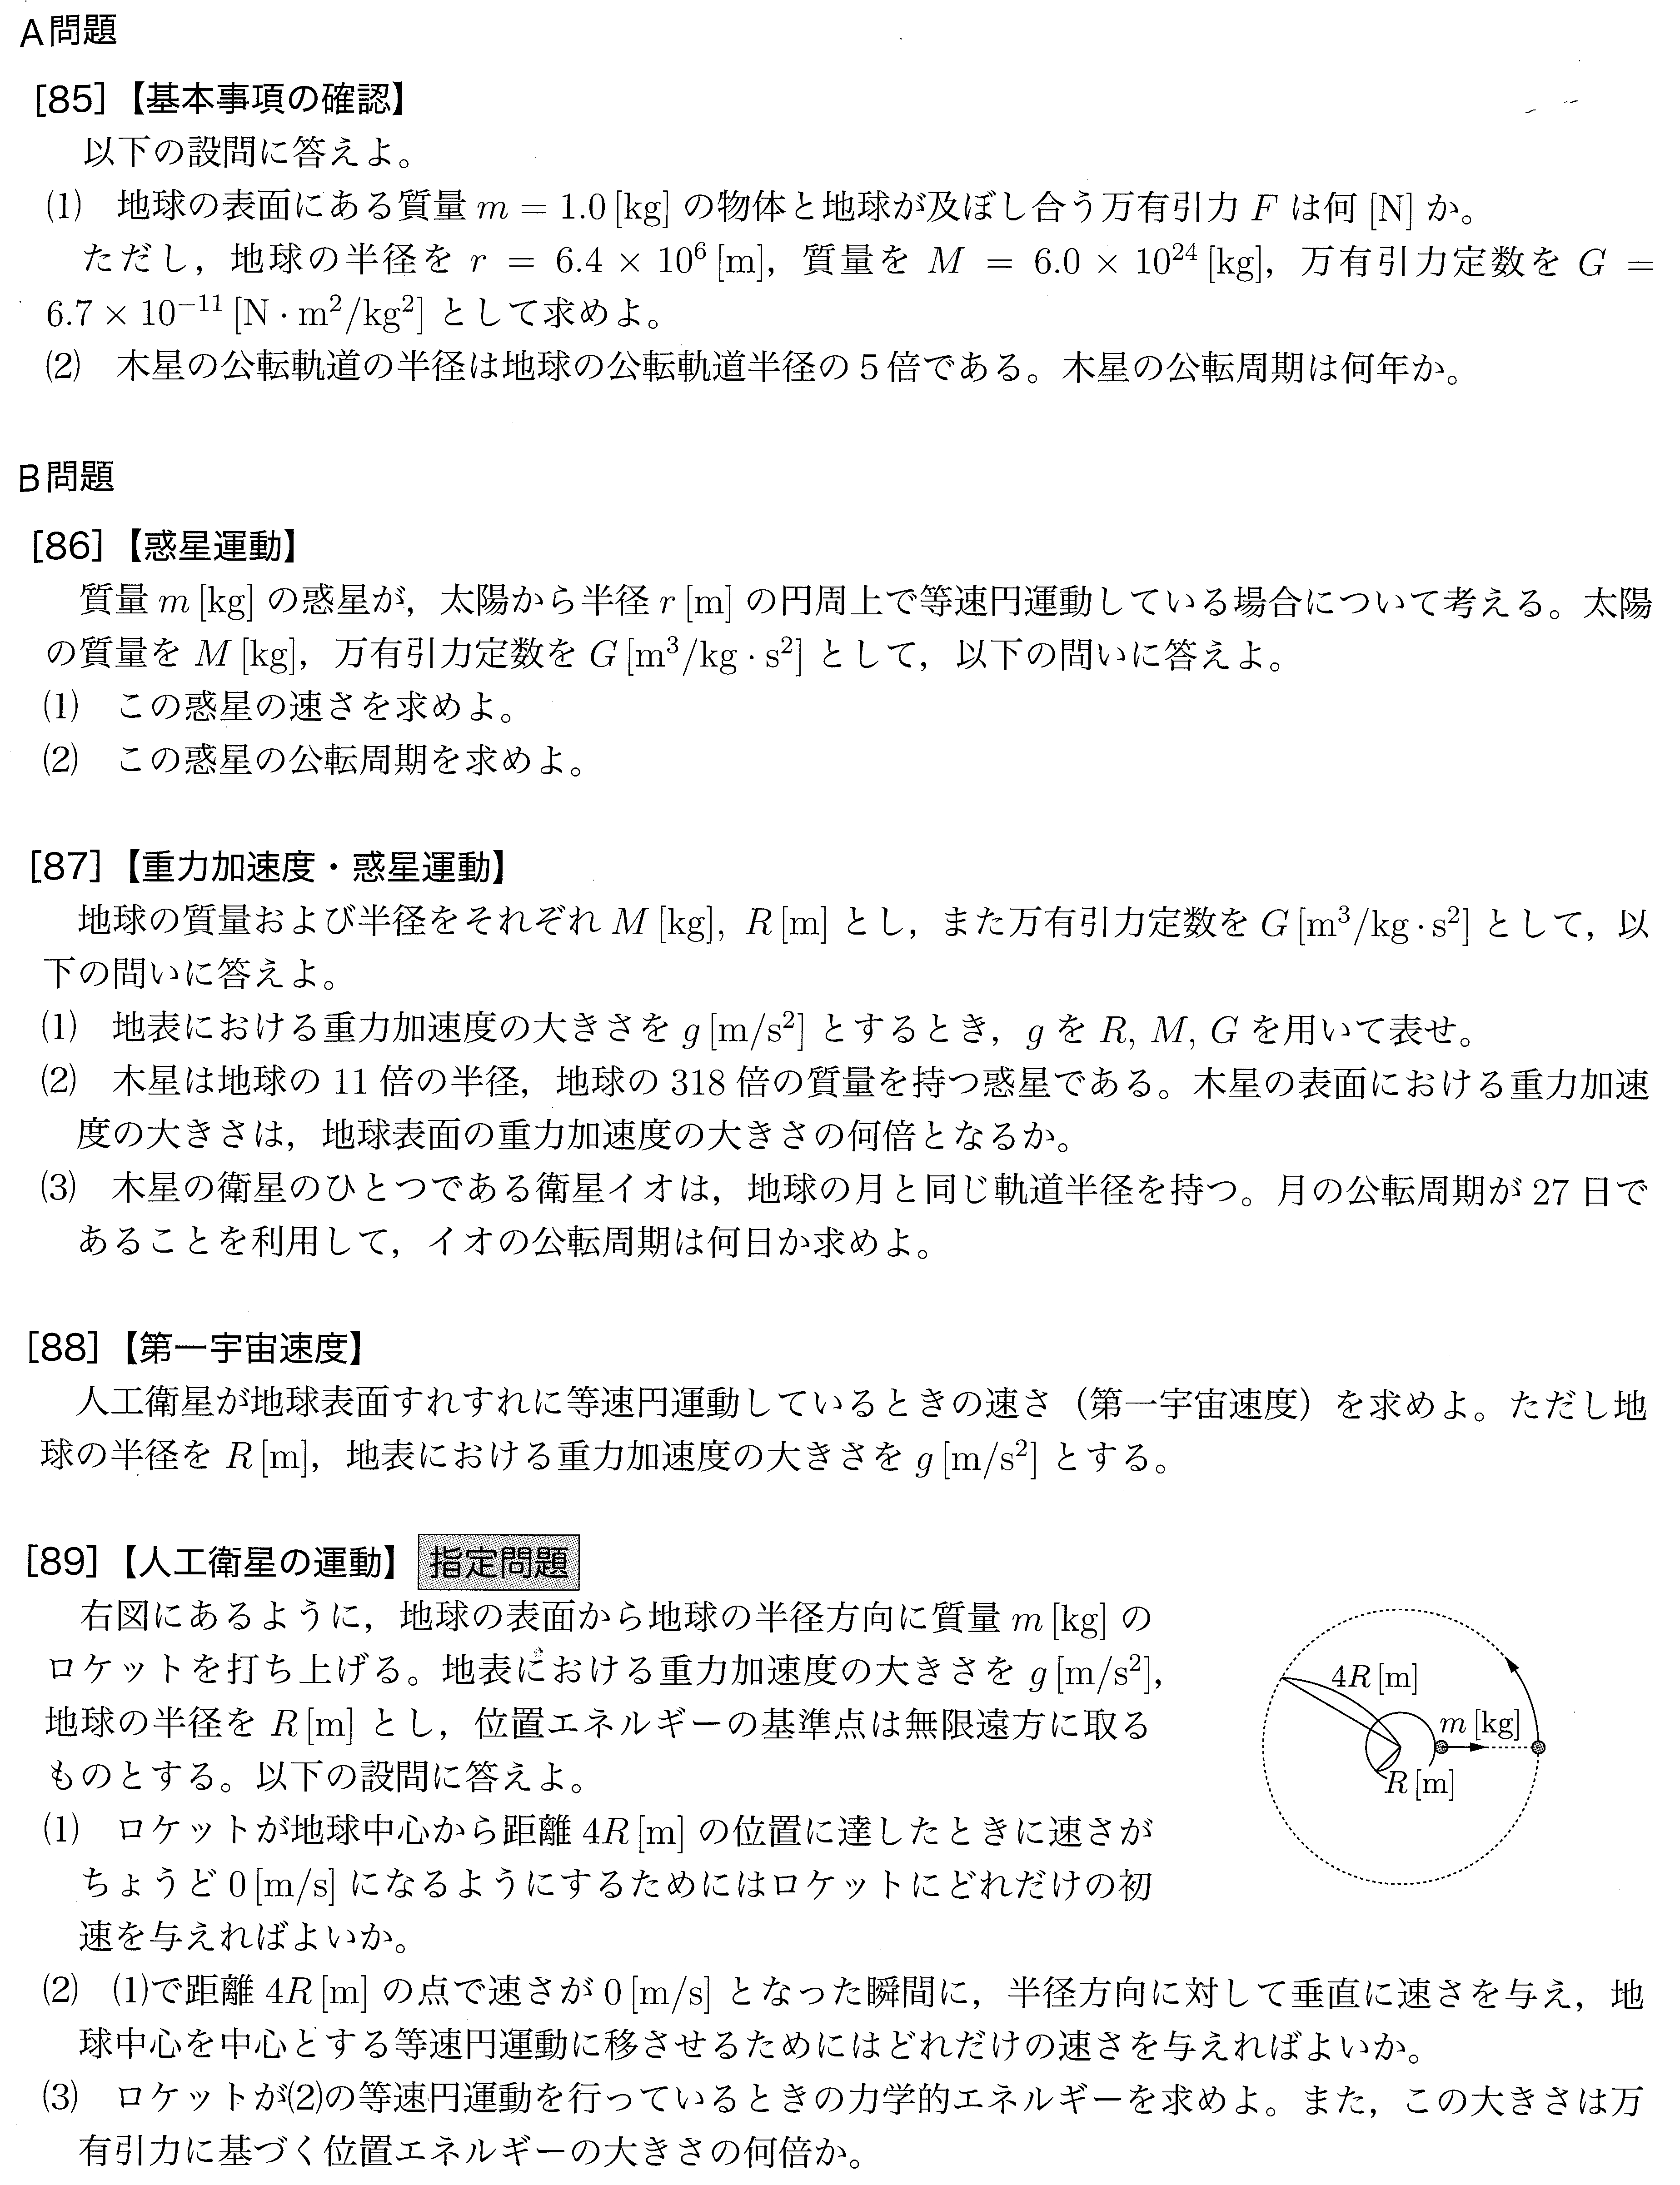
\includegraphics[width=170mm]{prob_p29.png}
\end{center}
\end{figure}

\newpage

\begin{figure}[h]
\begin{center}
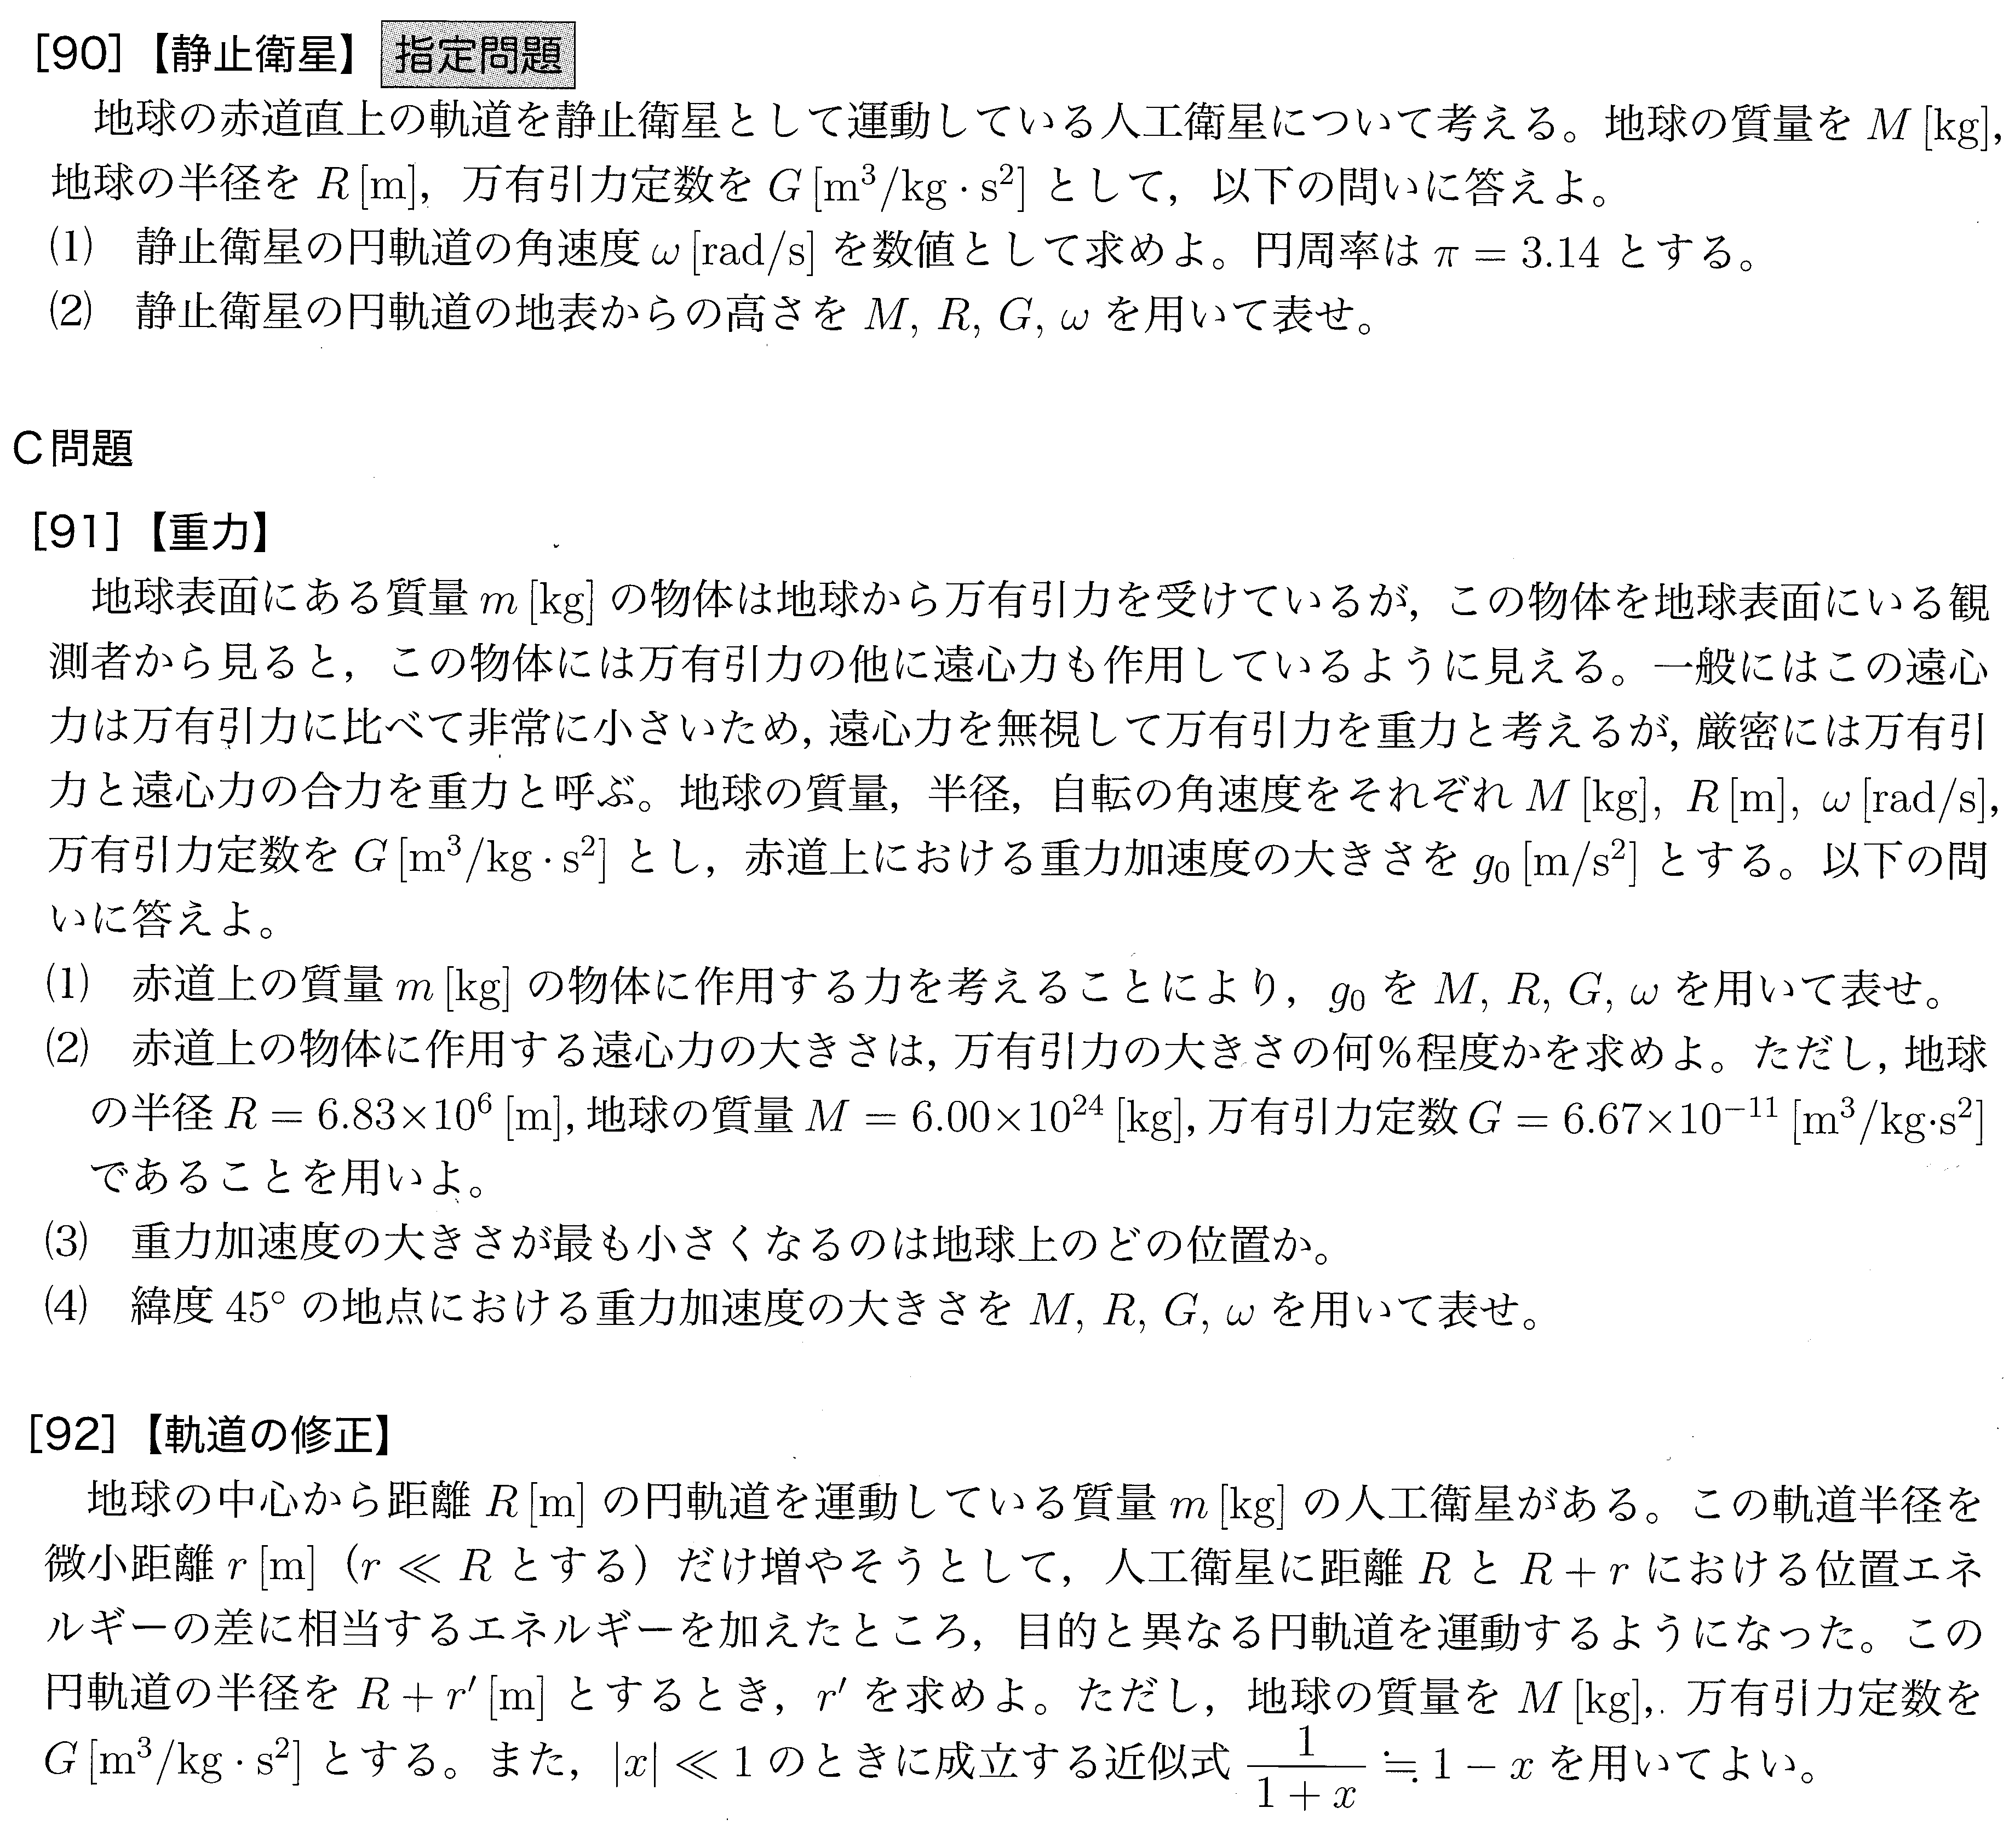
\includegraphics[width=170mm]{prob_p30.png}
\vspace{10cm}
\end{center}
\end{figure}



\newpage

\begin{figure}[h]
\begin{center}
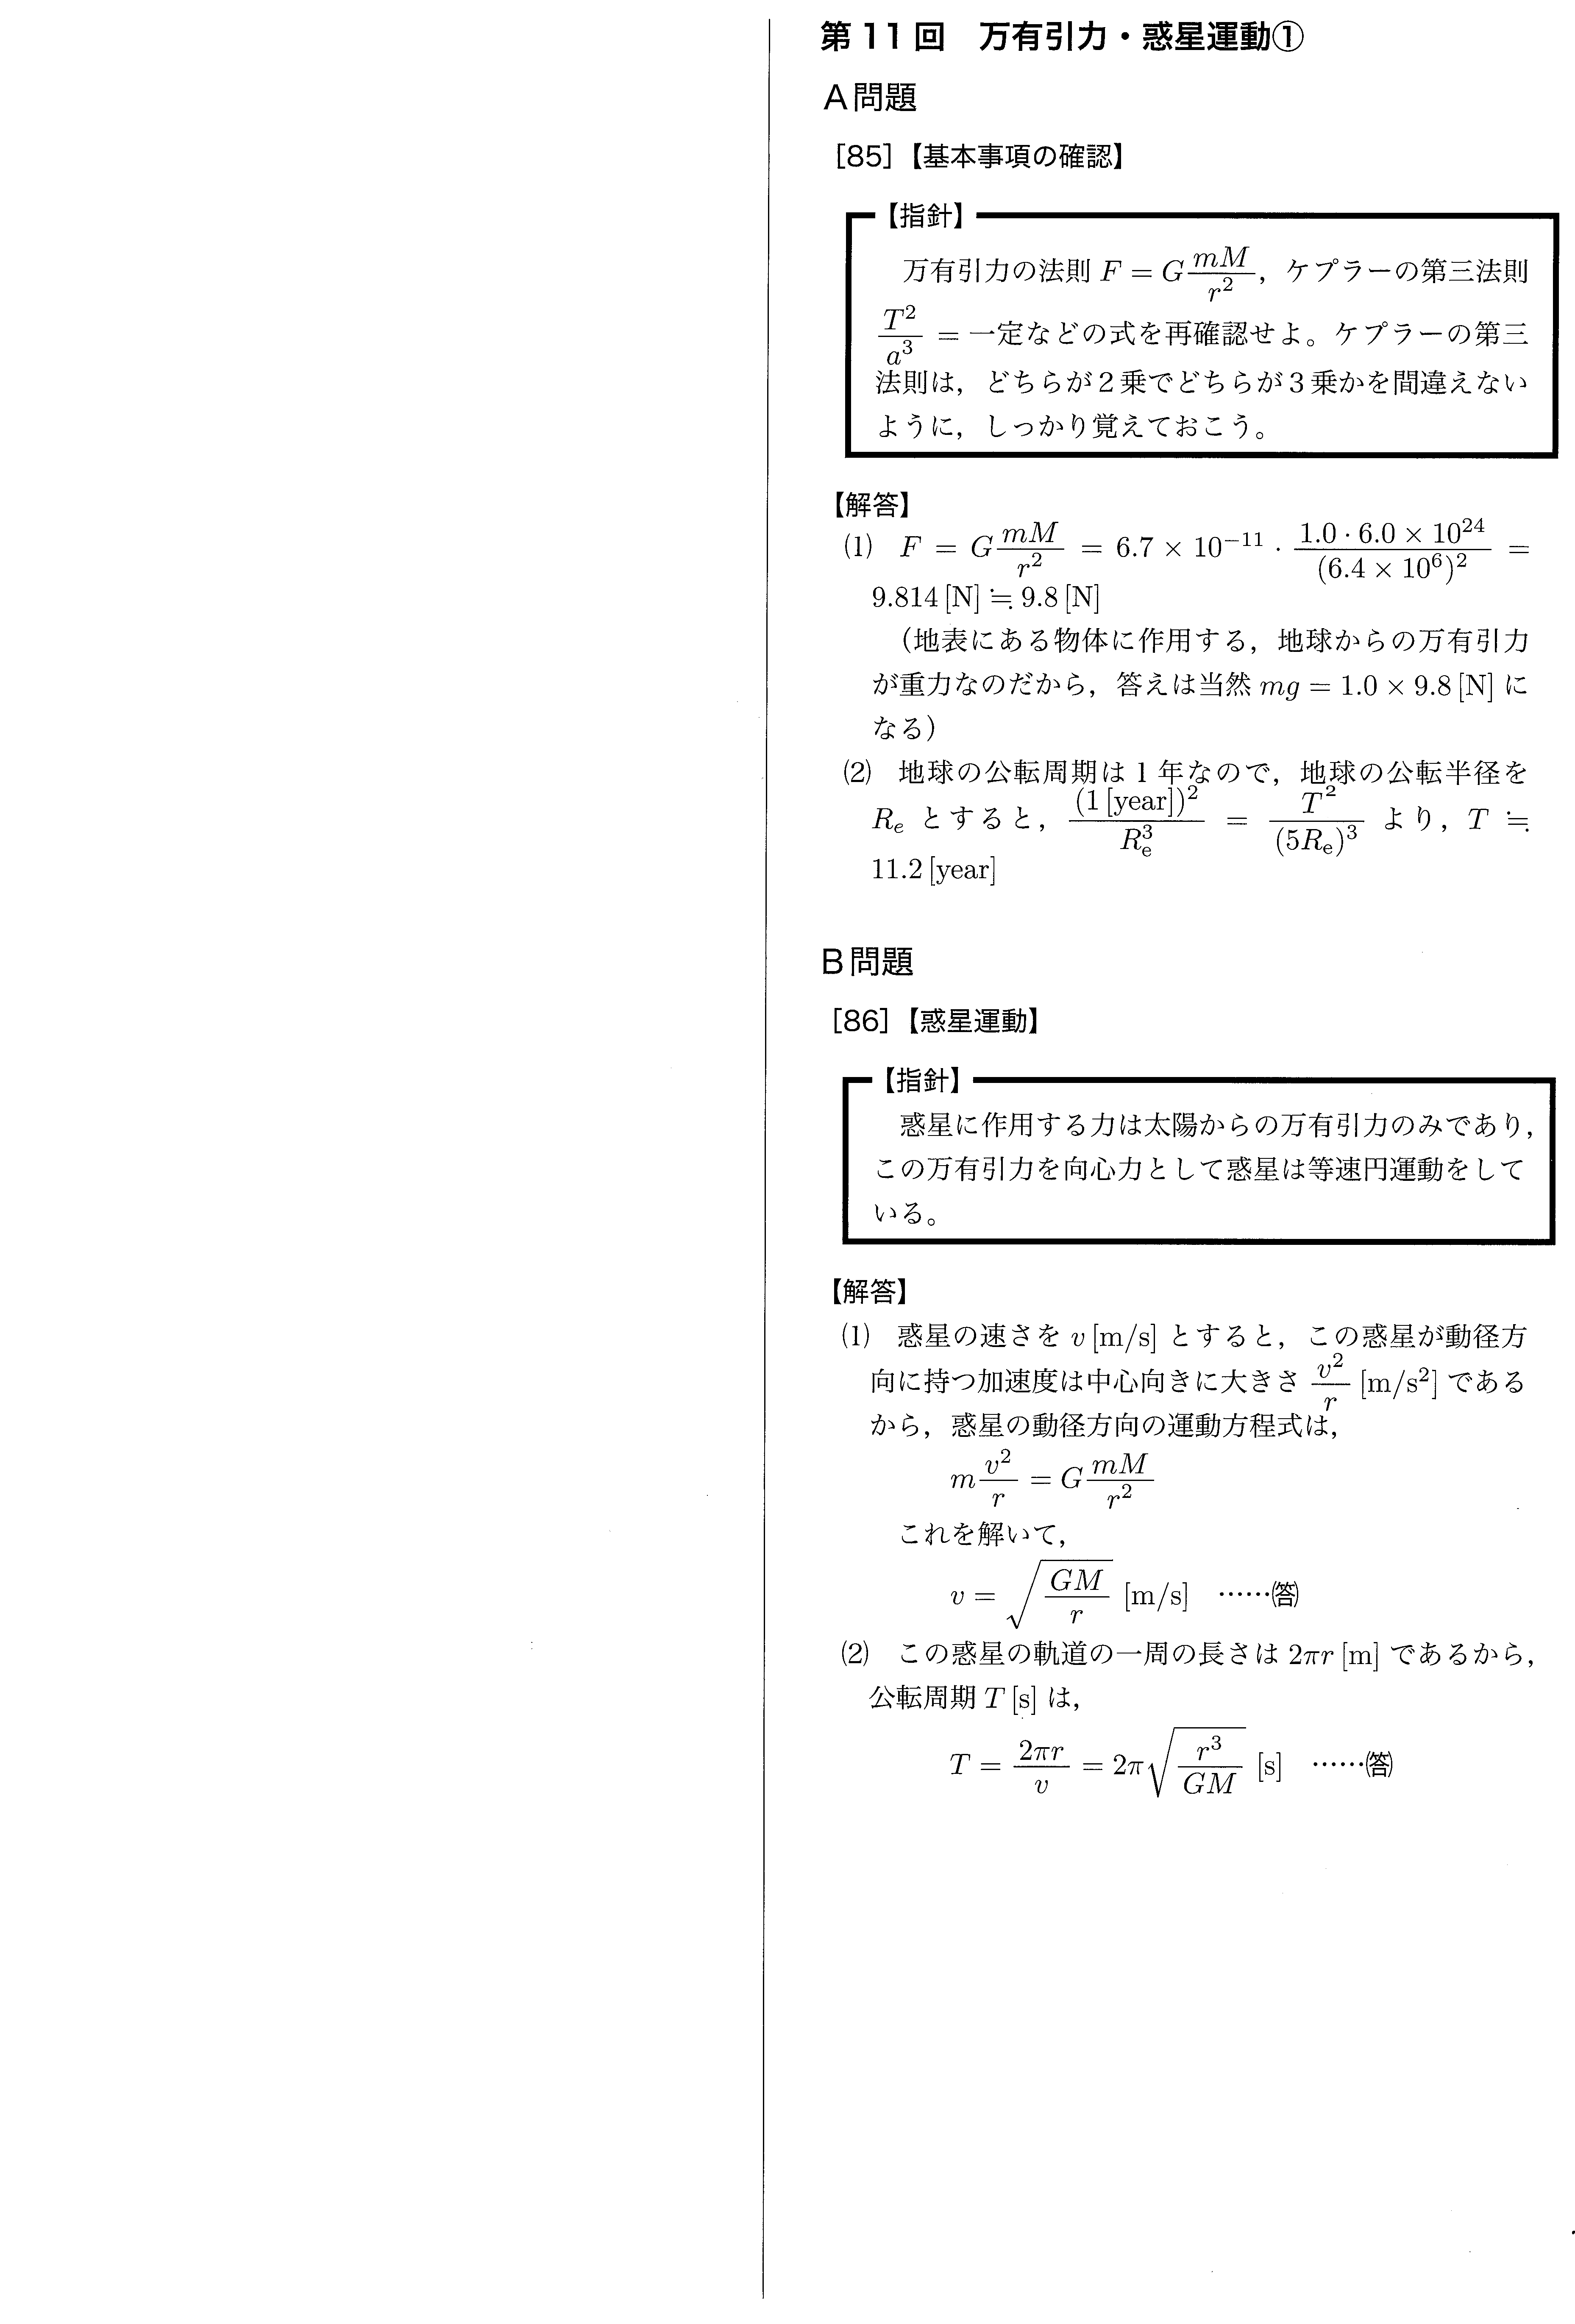
\includegraphics[width=170mm]{prob_p105_2.png}
\vspace{20cm}
\end{center}
\end{figure}

\newpage

\begin{figure}[h]
\begin{center}
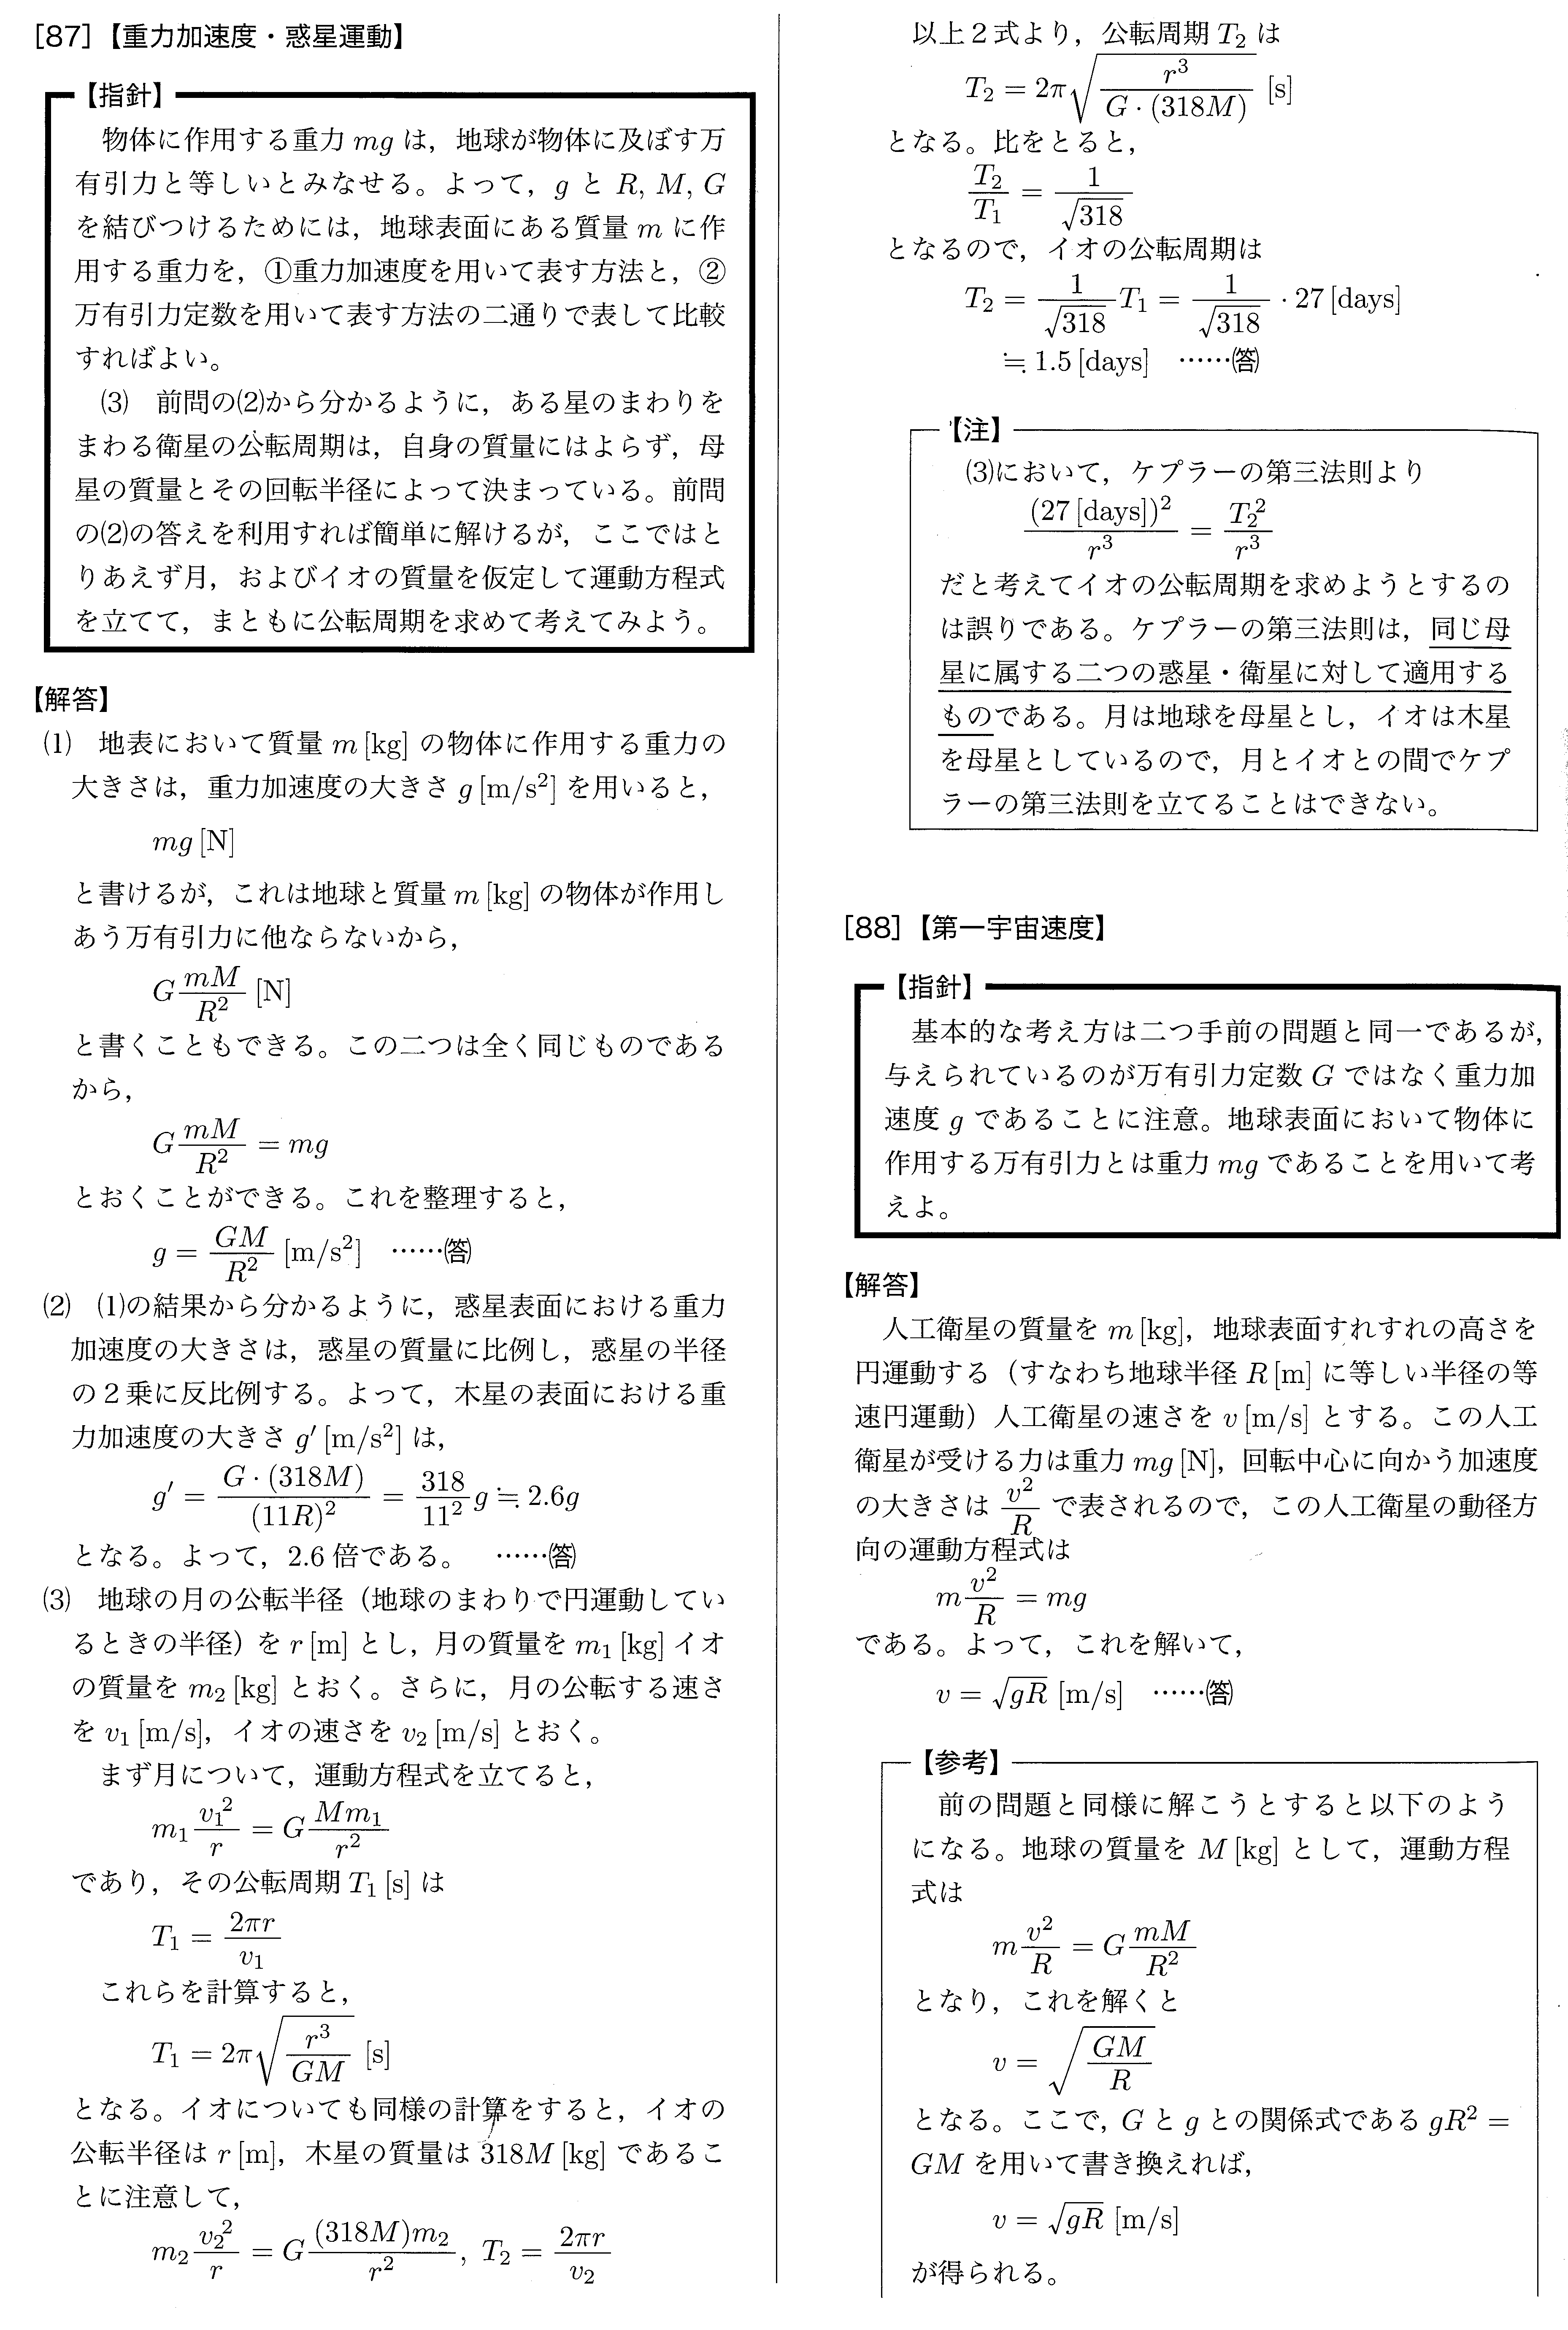
\includegraphics[width=170mm]{prob_p106.png}
\end{center}
\end{figure}

\newpage

\begin{figure}[h]
\begin{center}
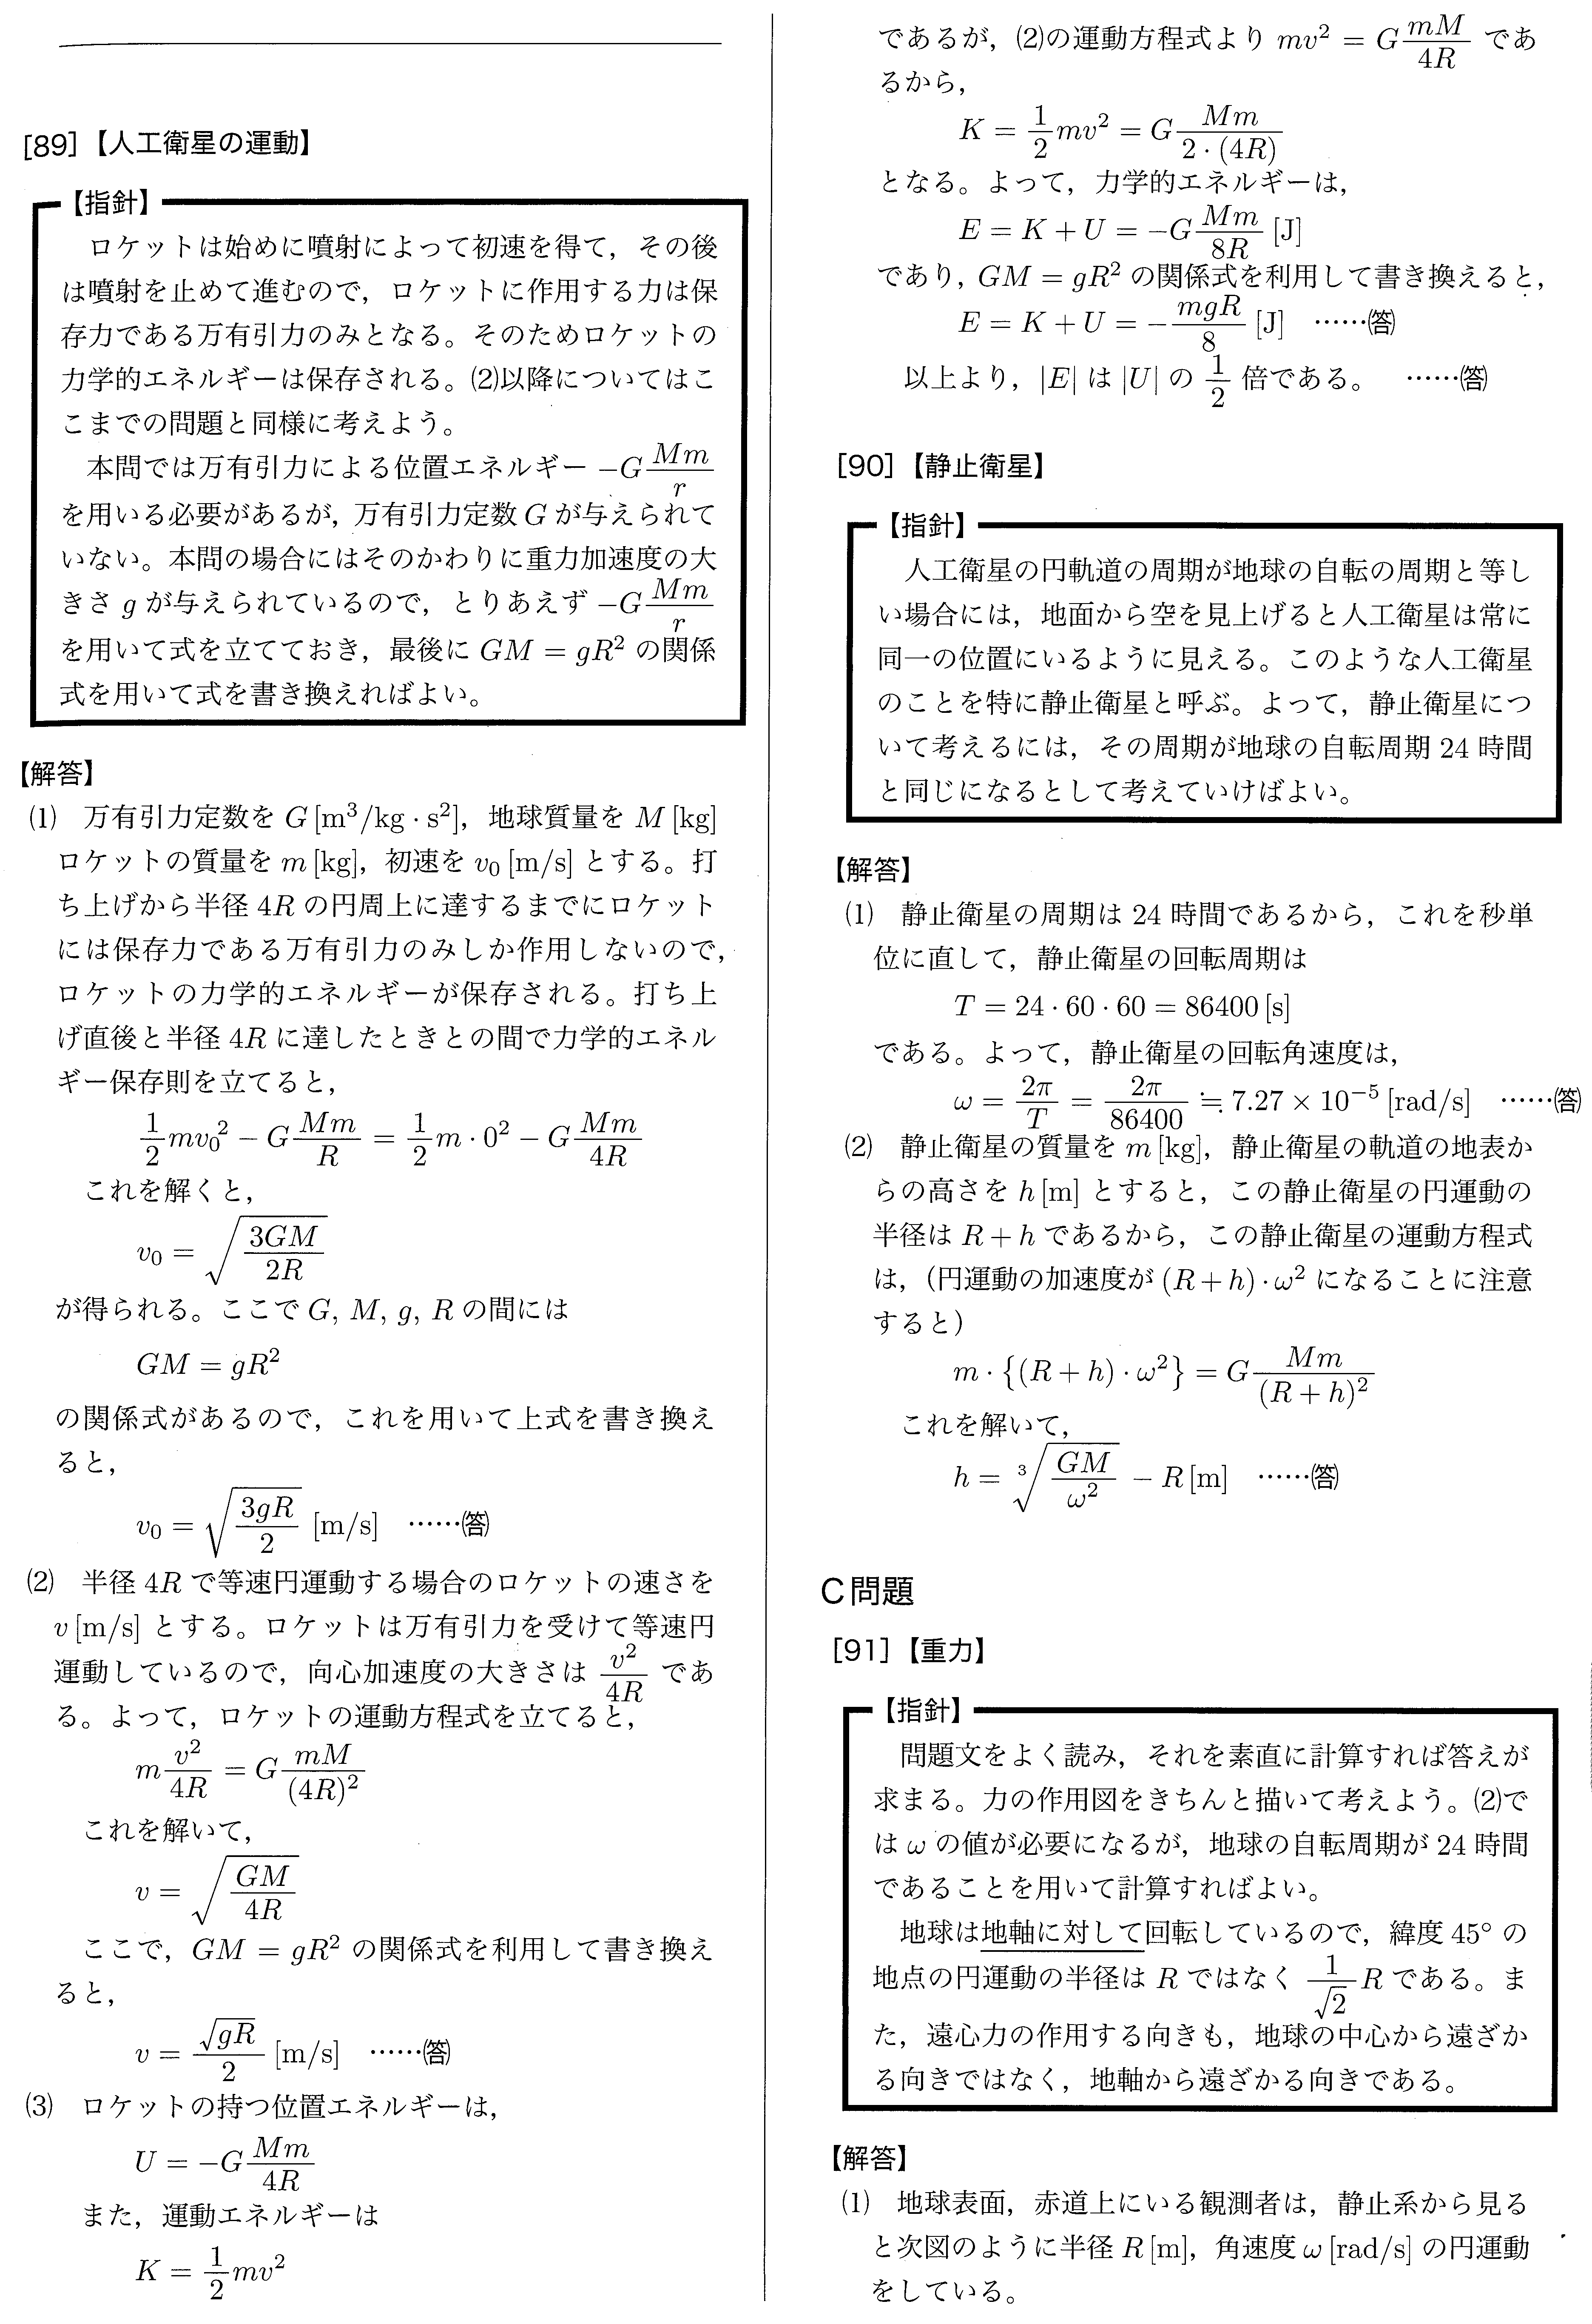
\includegraphics[width=170mm]{prob_p107.png}
\end{center}
\end{figure}
 
 \newpage

\begin{figure}[h]
\begin{center}
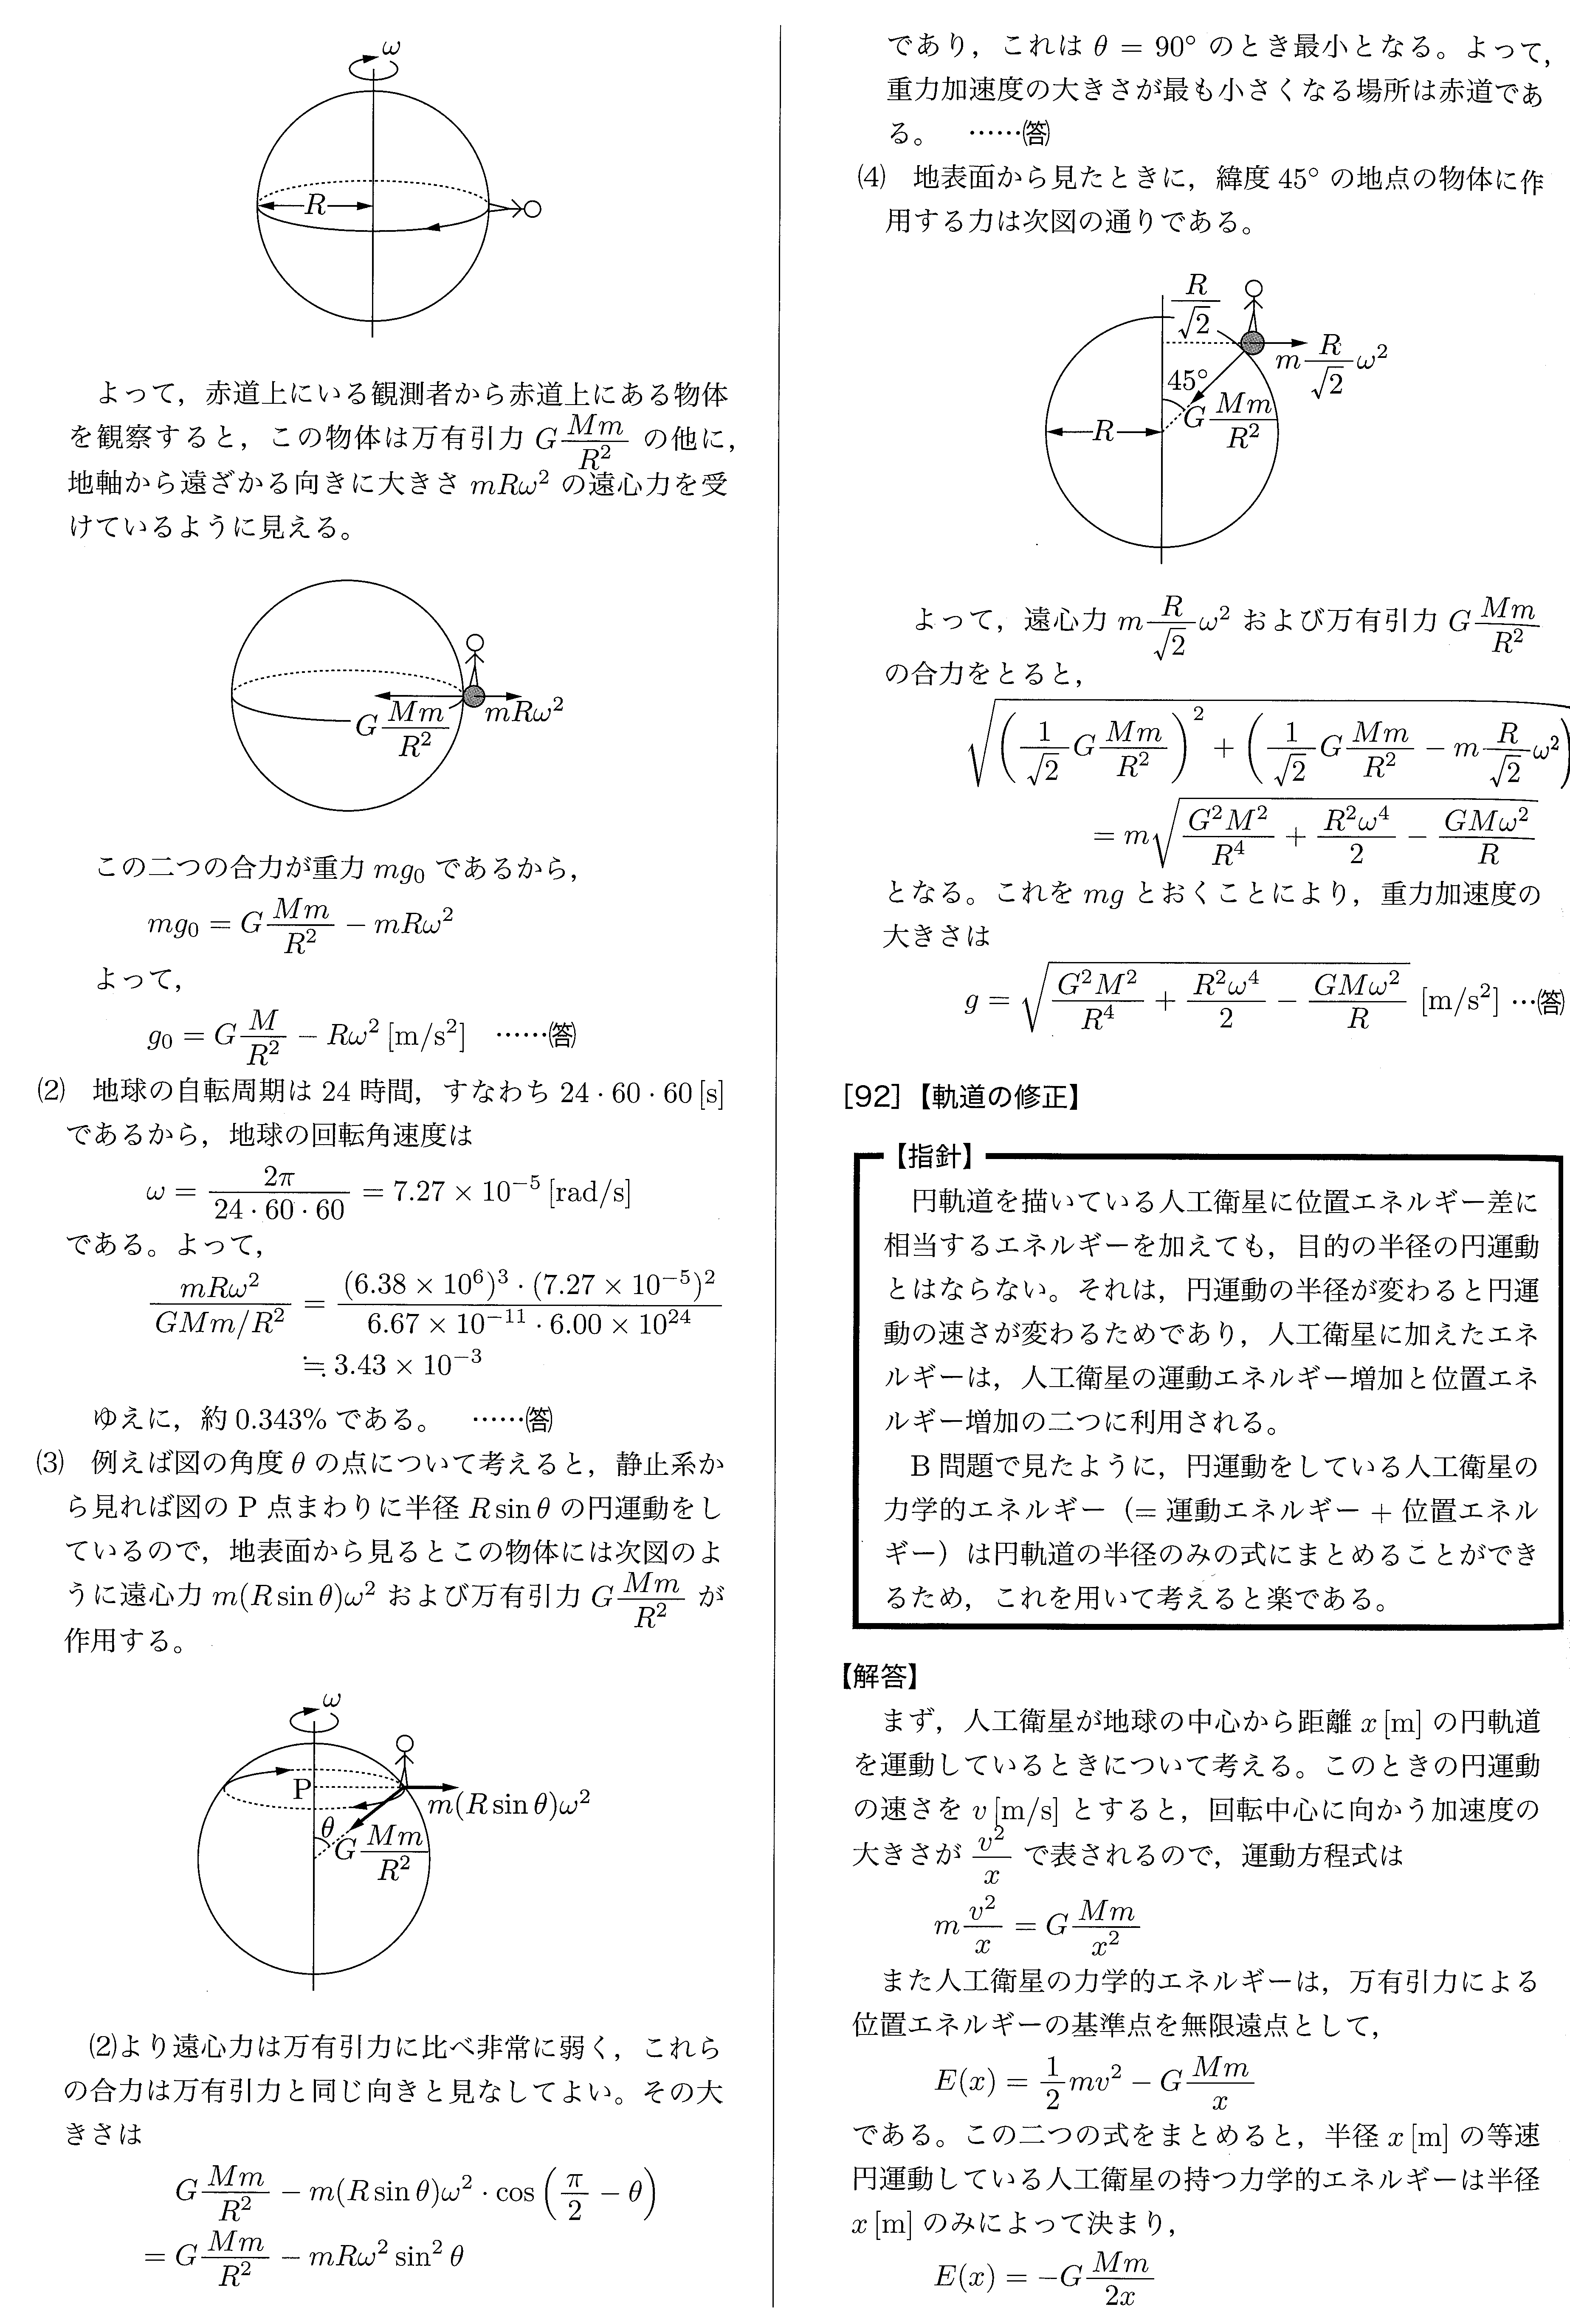
\includegraphics[width=170mm]{prob_p108.png}
\end{center}
\end{figure}

\newpage

\begin{figure}[h]
\begin{center}
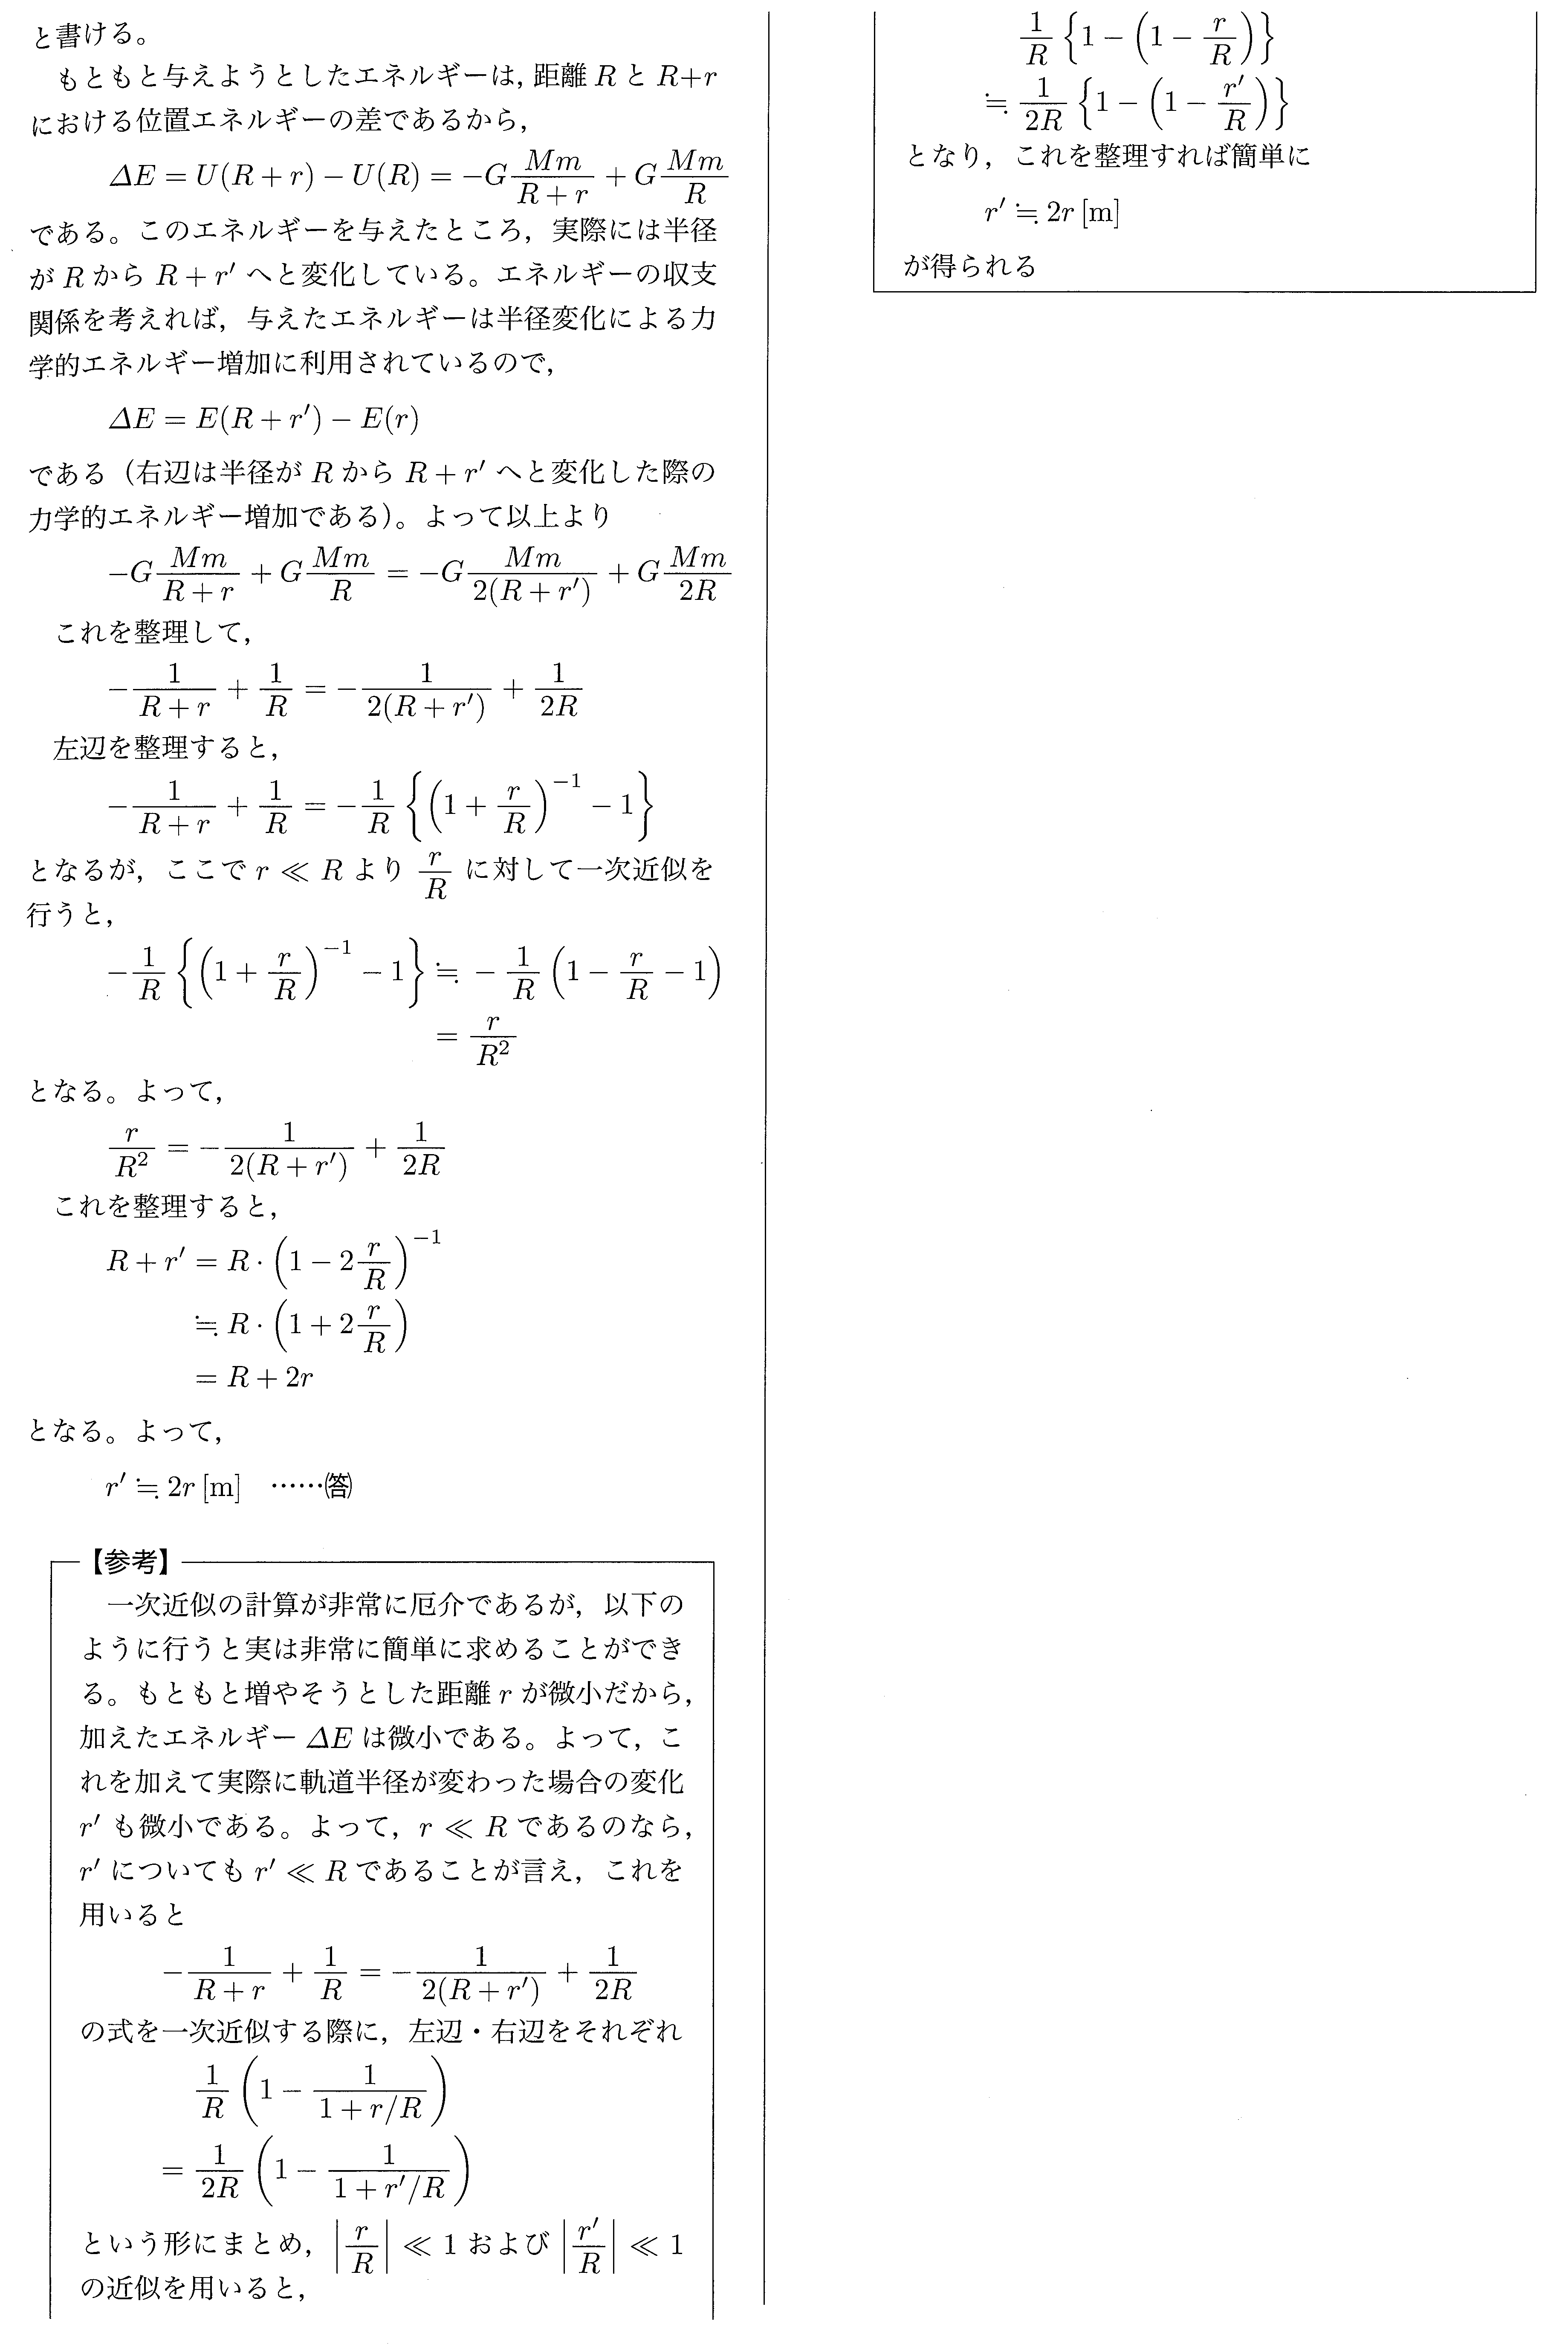
\includegraphics[width=170mm]{prob_p109.png}
\end{center}
\end{figure}


 
 \ 
 
\newpage
\include{physics_ch12}
\section{剛体のつり合い（2）}

\subsection{偶力}

\begin{wrapfigure}[10]{r}[5mm]{35mm}
  \centering
  \vspace{-5mm}
  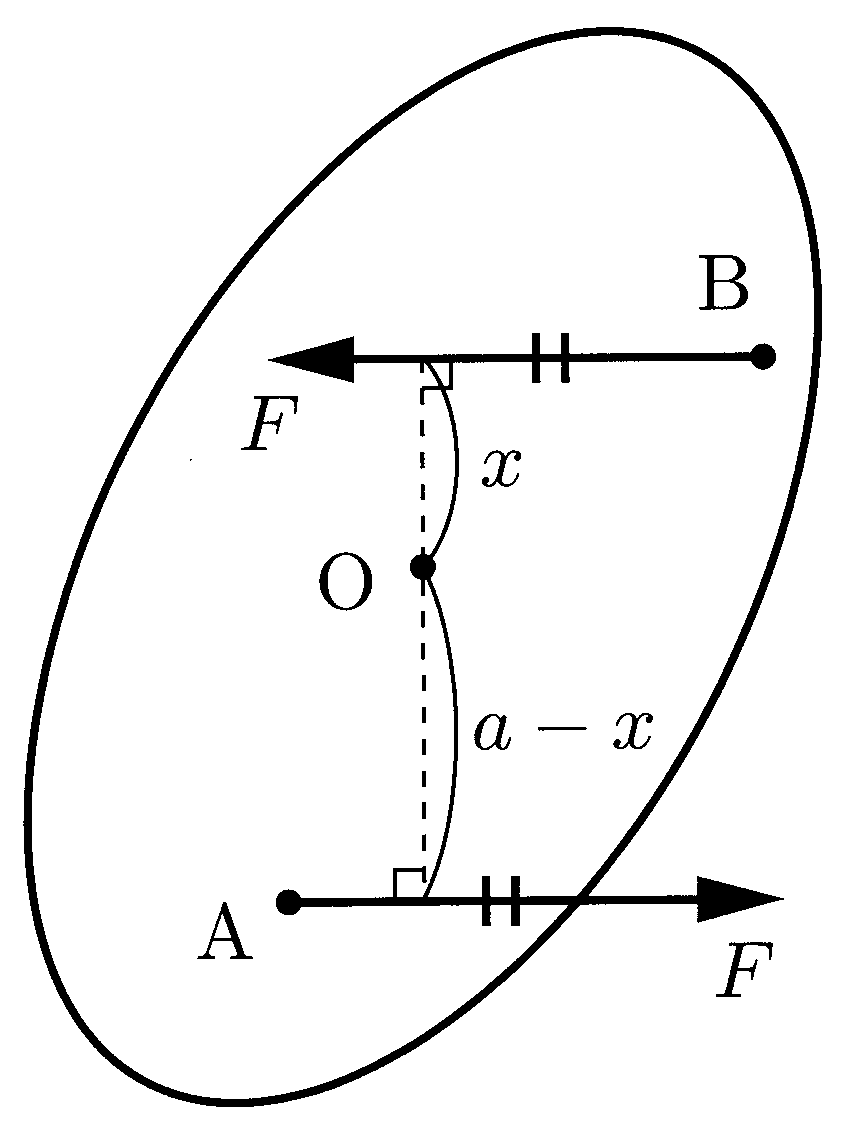
\includegraphics[keepaspectratio,width=35mm]
  {text_p60_fig1.png}
\end{wrapfigure}

ここまでで剛体に作用する力の合成方法を学んだが，大きさが同じで互いに逆向きの力については，力の作用点を結ぶ線分1：1に外分する点は存在しないから，この2つの力を合成することはできない．
そこで，このような2つの力は一組として考え，これを{\bf 偶力}という．

偶力の作用線間の距離を$a$[m]，片方の作用線から回転軸Oまでの距離を$x$[m]，力の大きさ$F$[N]とすると，この回転軸まわりの力のモーメントの和は
\[ N=F・x=F・(a-x)=Fa\]
となり，$x$に依存しない．
すなわち，{\bf 回転軸のどの位置をとっても，その回転軸のまわりの偶力のモーメントは一定である．}

一般に，回転軸Oまわりの力のモーメントは$N=F_\perp r$であり，力のうちの垂直成分が剛体を回転させる作用を持ち，平行成分は回転軸を動かそうとする力，すなわち剛体を移動させる作用を持っている．
これに対して偶力はどの回転軸まわりに対しても剛体を回転させる作用のみしか持たない．

\begin{matome}{偶力のモーメント}
 \hspace{3mm} 大きさ$F$[N]の2力が平行で互いに逆向きに作用しているとき，この一組を偶力という．\\
\hspace{3mm}偶力のモーメントは，作用線間の距離を$a$とすると，\\
\[ N=Fa\]
\hspace{3mm}で与えられ，回転軸の位置によらない．
 \end{matome}

\subsection{重心}

\begin{wrapfigure}[14]{r}[5mm]{80mm}
  \centering
  \vspace{-5mm}
  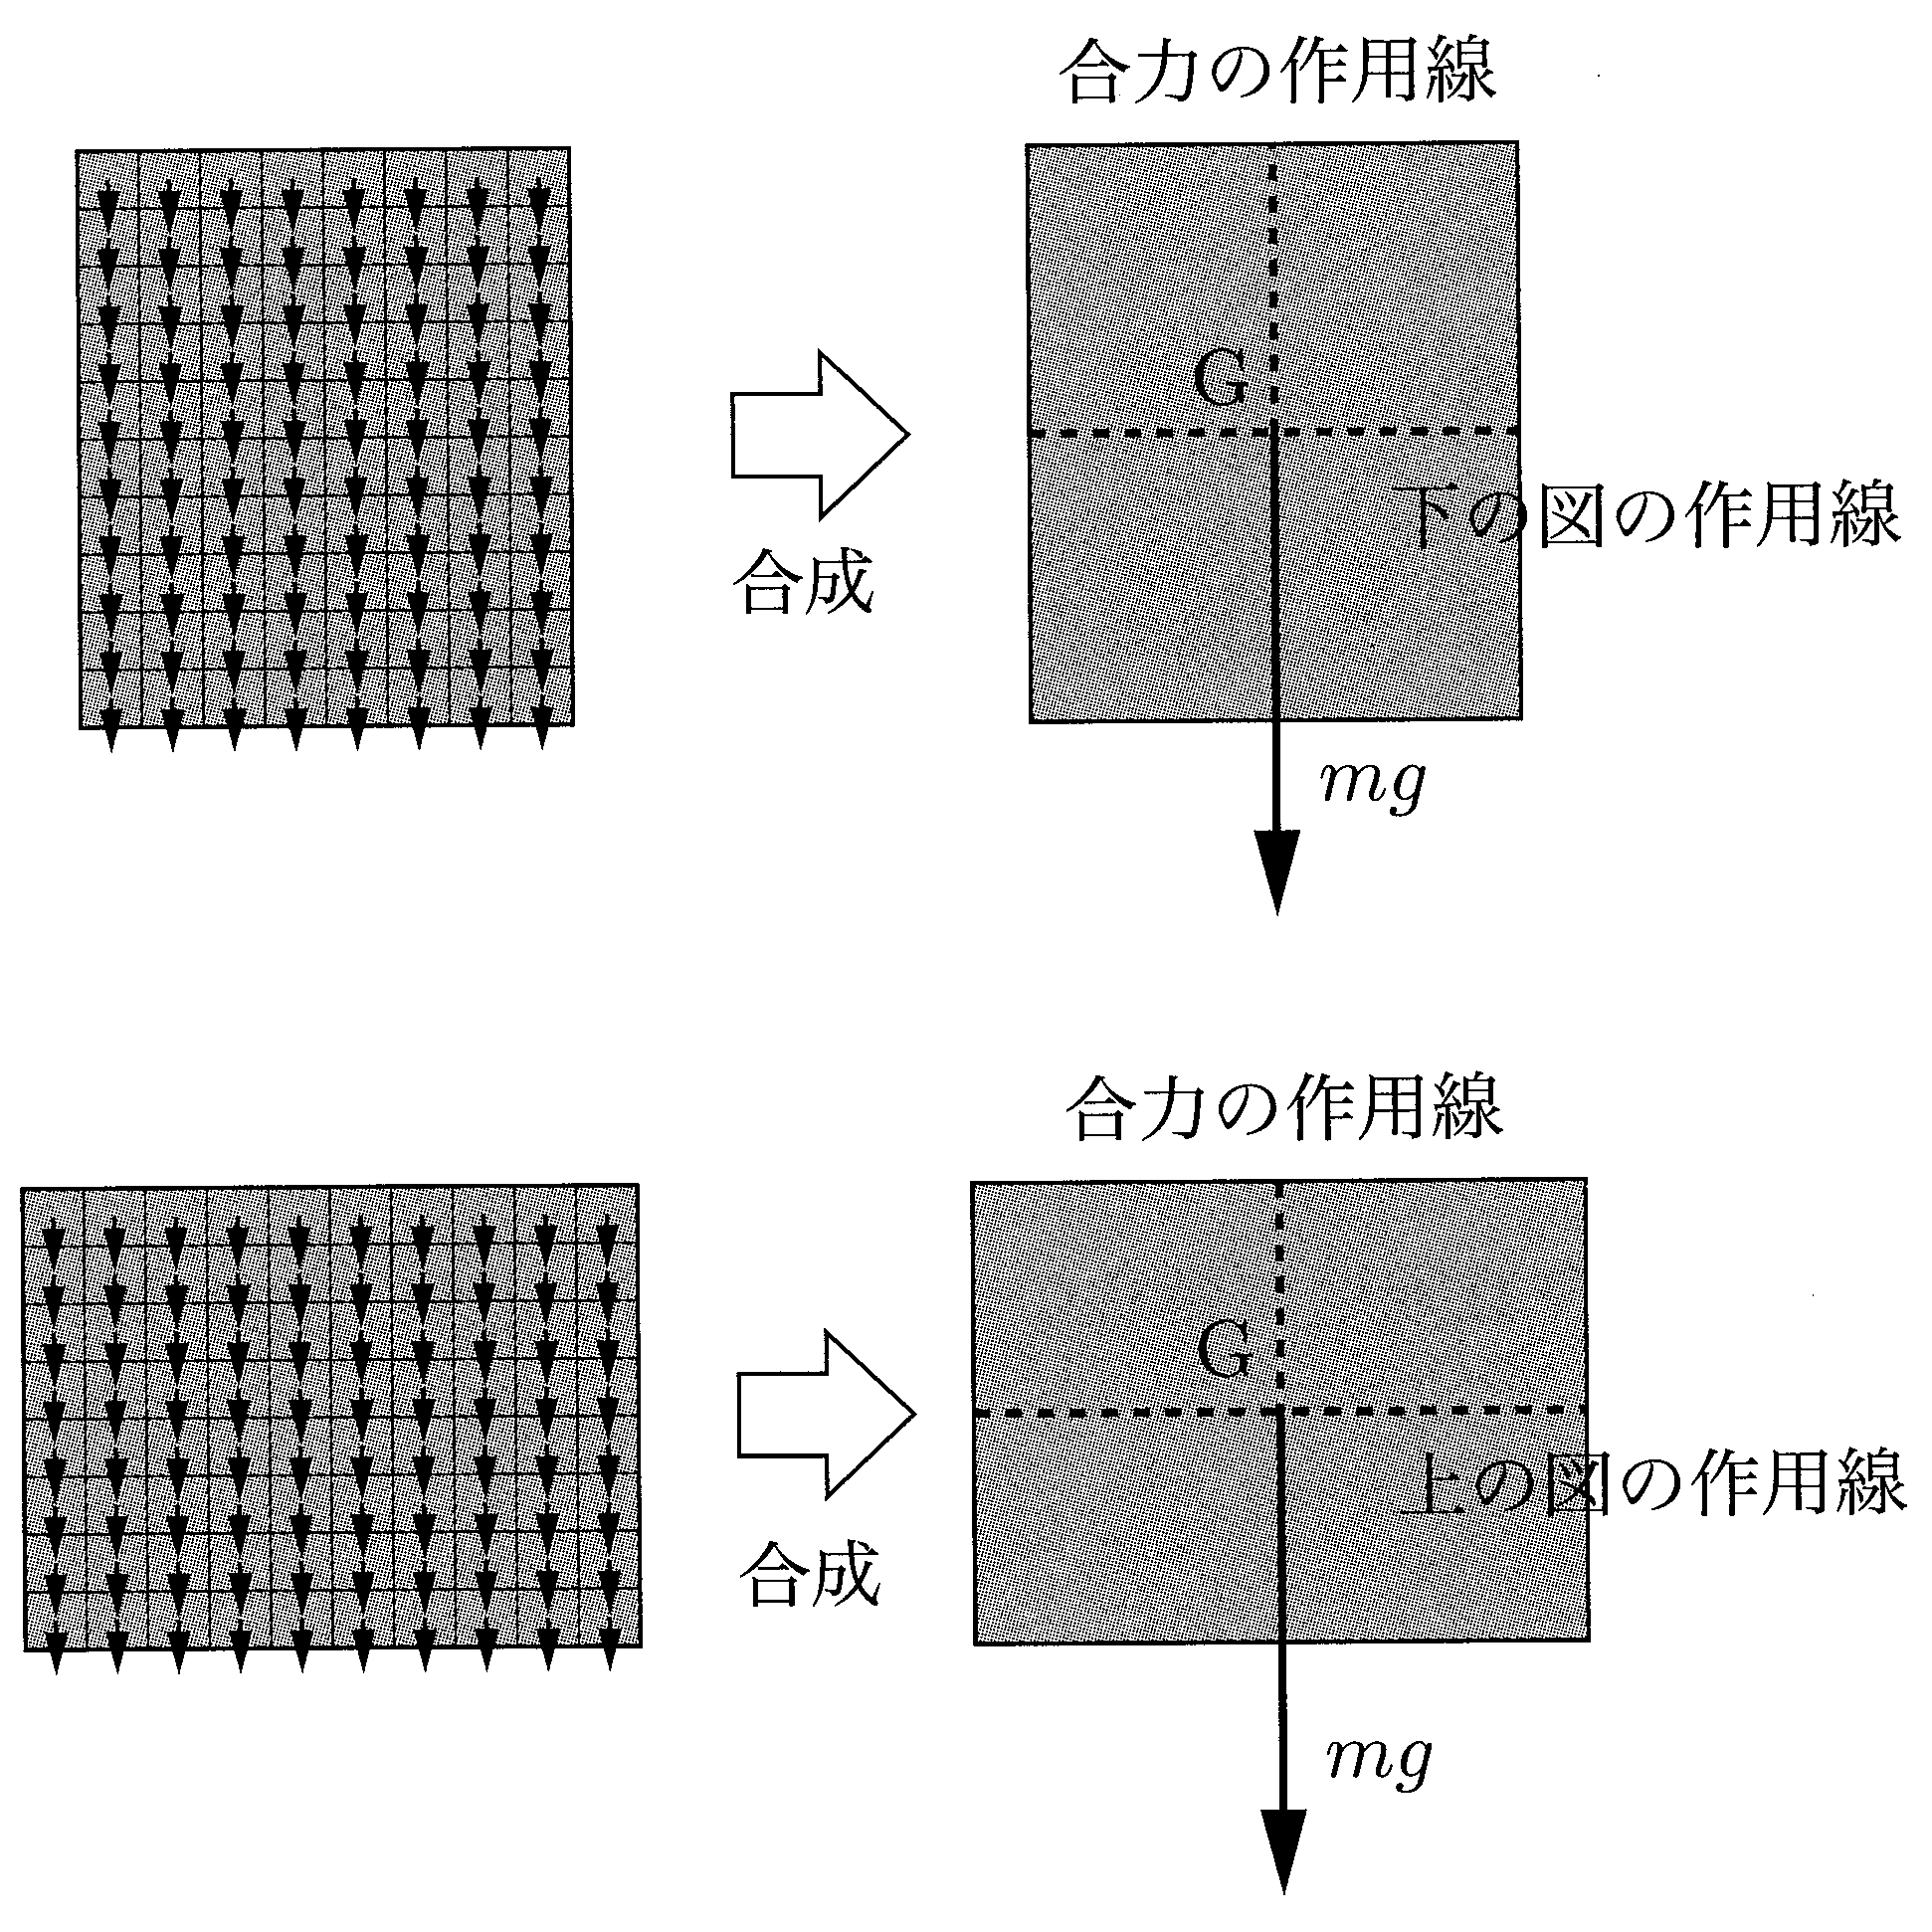
\includegraphics[keepaspectratio,width=75mm]
  {text_p60_fig2.png}
\end{wrapfigure}

ここまでにおいて，物体に作用する重力は物体の中心に対して作用すると考えてきたが，厳密には大きさのある物体に対して作用する重力は，右図のように物体の各微小部分ごとに対してそれぞれ鉛直下向きに作用している．しかし各微小部分に作用する重力は全て平行かつ同じ向きになっているので，12.2で学習した剛体に作用する平行力の合成の方法に従って必ずひとつの力に合成することができる．

合成した力の大きさは，物体の質量が$m$[kg]であれば常に$mg$[N]となるが，その作用線は物体の向きによって変化する．
しかしその作用線は，物体の向きによらず必ずある一点を通過することが知られており，この点を{\bf 重心}という．


\begin{wrapfigure}[8]{r}[5mm]{60mm}
  \centering
  \vspace{-5mm}
  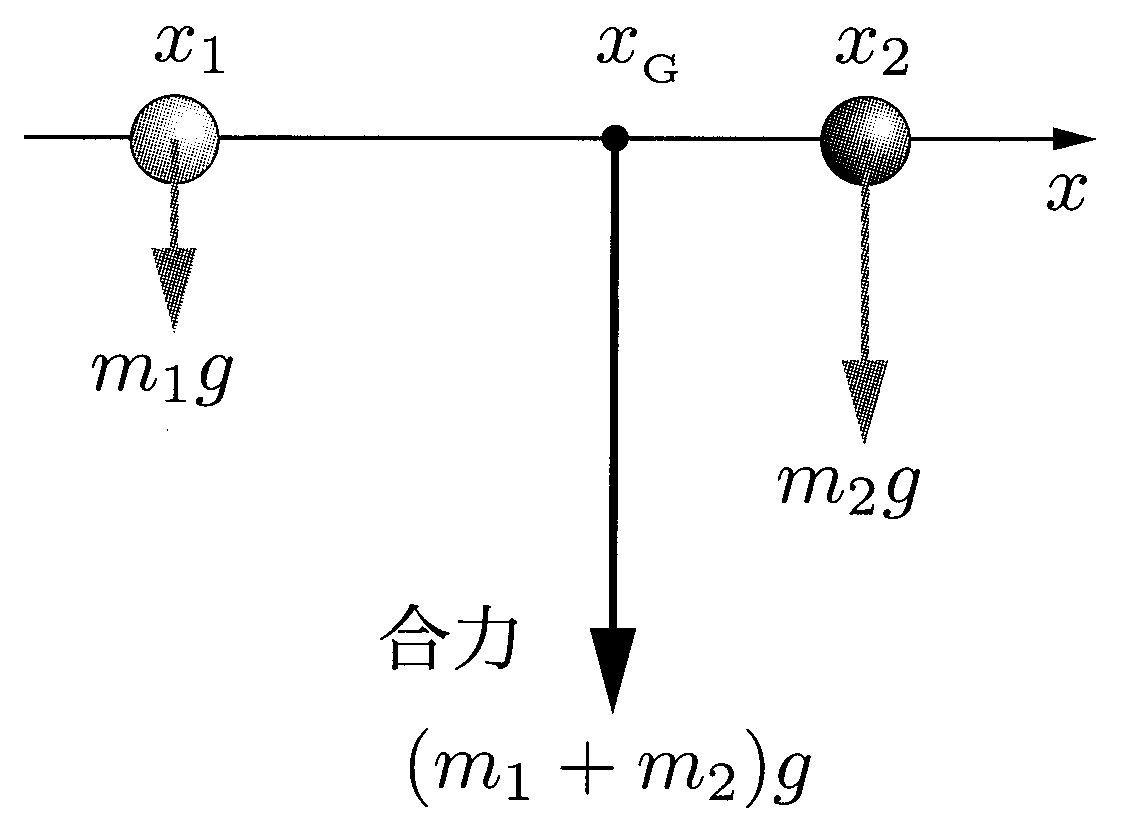
\includegraphics[keepaspectratio,width=55mm]
  {text_p61_fig1.png}
\end{wrapfigure}

物体の重心位置を求めるためには次のようにすればよい．
上図にあるようにまず物体を微小部分に分割し，各微小部分に対してかかる重力を合成してその作用線を求める．
これを$x,y$軸の2方向について行い，その作用線の交点を取ればよい．

各部分にかかる多数の重力を合成するには2つずつ順番に合成していけばよいので，とりあえず座標$x_1,x_2$[m]に置かれている質量$m_1,m_2$[kg]の物体に作用する重力の合成を行ってみよう．
この場合，大きさ$(m_1+m_2)g$[N]の力が線分を$m_2:m_1$に内分する点Gに作用することになる．
よって，この場合の重心位置Gは内分公式を用いて，
\[ x_G=\dfrac{m_1x_1+m_2x_2}{m_1+m_2} \hspace{2mm}{\rm [m]}\]
として求めることができる．
さらにこのGに対して他の微小部分に作用する重力を合成していくことにより，全重力の合力の作用点，すなわち物体の重心座標を求めることができ，その点は$n$個の物体であれば
\[ x_G=\dfrac{m_1x_1+m_2x_2+\cdots +m_nx_n}{m_1+m_2+\cdots +m_n} \hspace{2mm}{\rm [m]}\]
の位置となる．

以上より，剛体がいかなる向きをとっていても剛体に作用する重力の全合力は，{\bf 重心に対して全質量分の重力が作用している}とだけ考えればよく，{\bf 重心まわりの重力のモーメントの和は必ず0となる}と言える．

一般的な物体の重心位置は，以上で述べたような複雑な手続きを踏む必要があるが，一様な密度を持つ物体の場合は幾何学的対称性から明らかなことが多い．
例えば一様な棒の重心はその中点に，また一様な円盤や正方形板，球の重心はその中心にある．

\begin{matome}{重心}
 \hspace{3mm} 剛体もしくは質点系に作用する重力を一点で支えたときに，剛体もしくは質点系の向きによらずにつり合いの条件を満たすことのできる点を重心という．その重心の座標は\\
\[ \overrightarrow{x_G\mathstrut}=\dfrac{m_1\overrightarrow{x_1\mathstrut}+m_2\overrightarrow{x_2\mathstrut}+\cdots +m_n\overrightarrow{x_n \mathstrut}}{m_1+m_2+\cdots +m_n} \hspace{2mm}{\rm [m]}\]
 \end{matome}


 \ 
 
%\begin{breakbox}
%\ex＜重心座標＞\\
%\begin{wrapfigure}[7]{r}[5mm]{60mm}
%  \centering
%%  \vspace{-5mm}
%  \includegraphics[keepaspectratio,width=53mm]
%  {text_p62_fig1.png}
%  \includegraphics[keepaspectratio,width=45mm]
%  {text_p62_fig2.png}
%\end{wrapfigure}
%\hspace{5mm}重心に関する以下の問いに答えよ．
%\begin{description}
%\item[(1)] $x$軸上の座標で$x=-2,1,3$[m]の各点に質量$2m,m,m$[kg]の物体がそれぞれ置かれている．この質点系の重心の位置を求めよ．
%\item[(2)] (1)において，重心の座標を$x=2$[m]の位置にするためには，$x=4$[m]の地点に新たにどれだけの質量の物体を置けばよいか求めよ．
%\item[(3)] 一辺の長さが$l$[m]，全質量が$4m$[kg]の薄く，均質な正方形の板がある．この板の右上$\dfrac{1}{4}$を図のように切り取った．図のように座標軸を取るとき，この残った部分の物体の重心位置を求めよ．
%\end{description}
%
%\end{breakbox}

% \newpage 
%
%\begin{breakbox}
%\ex＜剛体のつり合い＞\\
%\begin{wrapfigure}[7]{r}[5mm]{50mm}
%  \centering
% \vspace{-5mm}
%  \includegraphics[keepaspectratio,width=40mm]
%  {text_p62_fig3.png}
%\end{wrapfigure}
%\hspace{5mm}長さ$l$[m]，質量$m$[kg]のかたくて一様な棒がある．この棒の下端を床にちょうつがいで止め，棒の上端につけた糸を引いて図のように角$\theta$でつり合わせて静止させることについて考える．重力加速度の大きさを$g {\rm [m/s^2]}$として以下の問いに答えよ．
%\begin{description}
%\item[(1)] 糸を水平に引いてつり合わせるためにはどれだけの大きさで引けばよいか．
%\item[(2)] 糸が棒と垂直をなすようにして引いてつり合わせるためにはどれだけの大きさで引けばよいか．
%\item[(3)] (2)のとき，ちょうつがいが棒に及ぼす力の水平成分および鉛直成分をそれぞれ求めよ．
%\end{description}
%
%\end{breakbox}


  \newpage

\begin{figure}[h]
\begin{center}
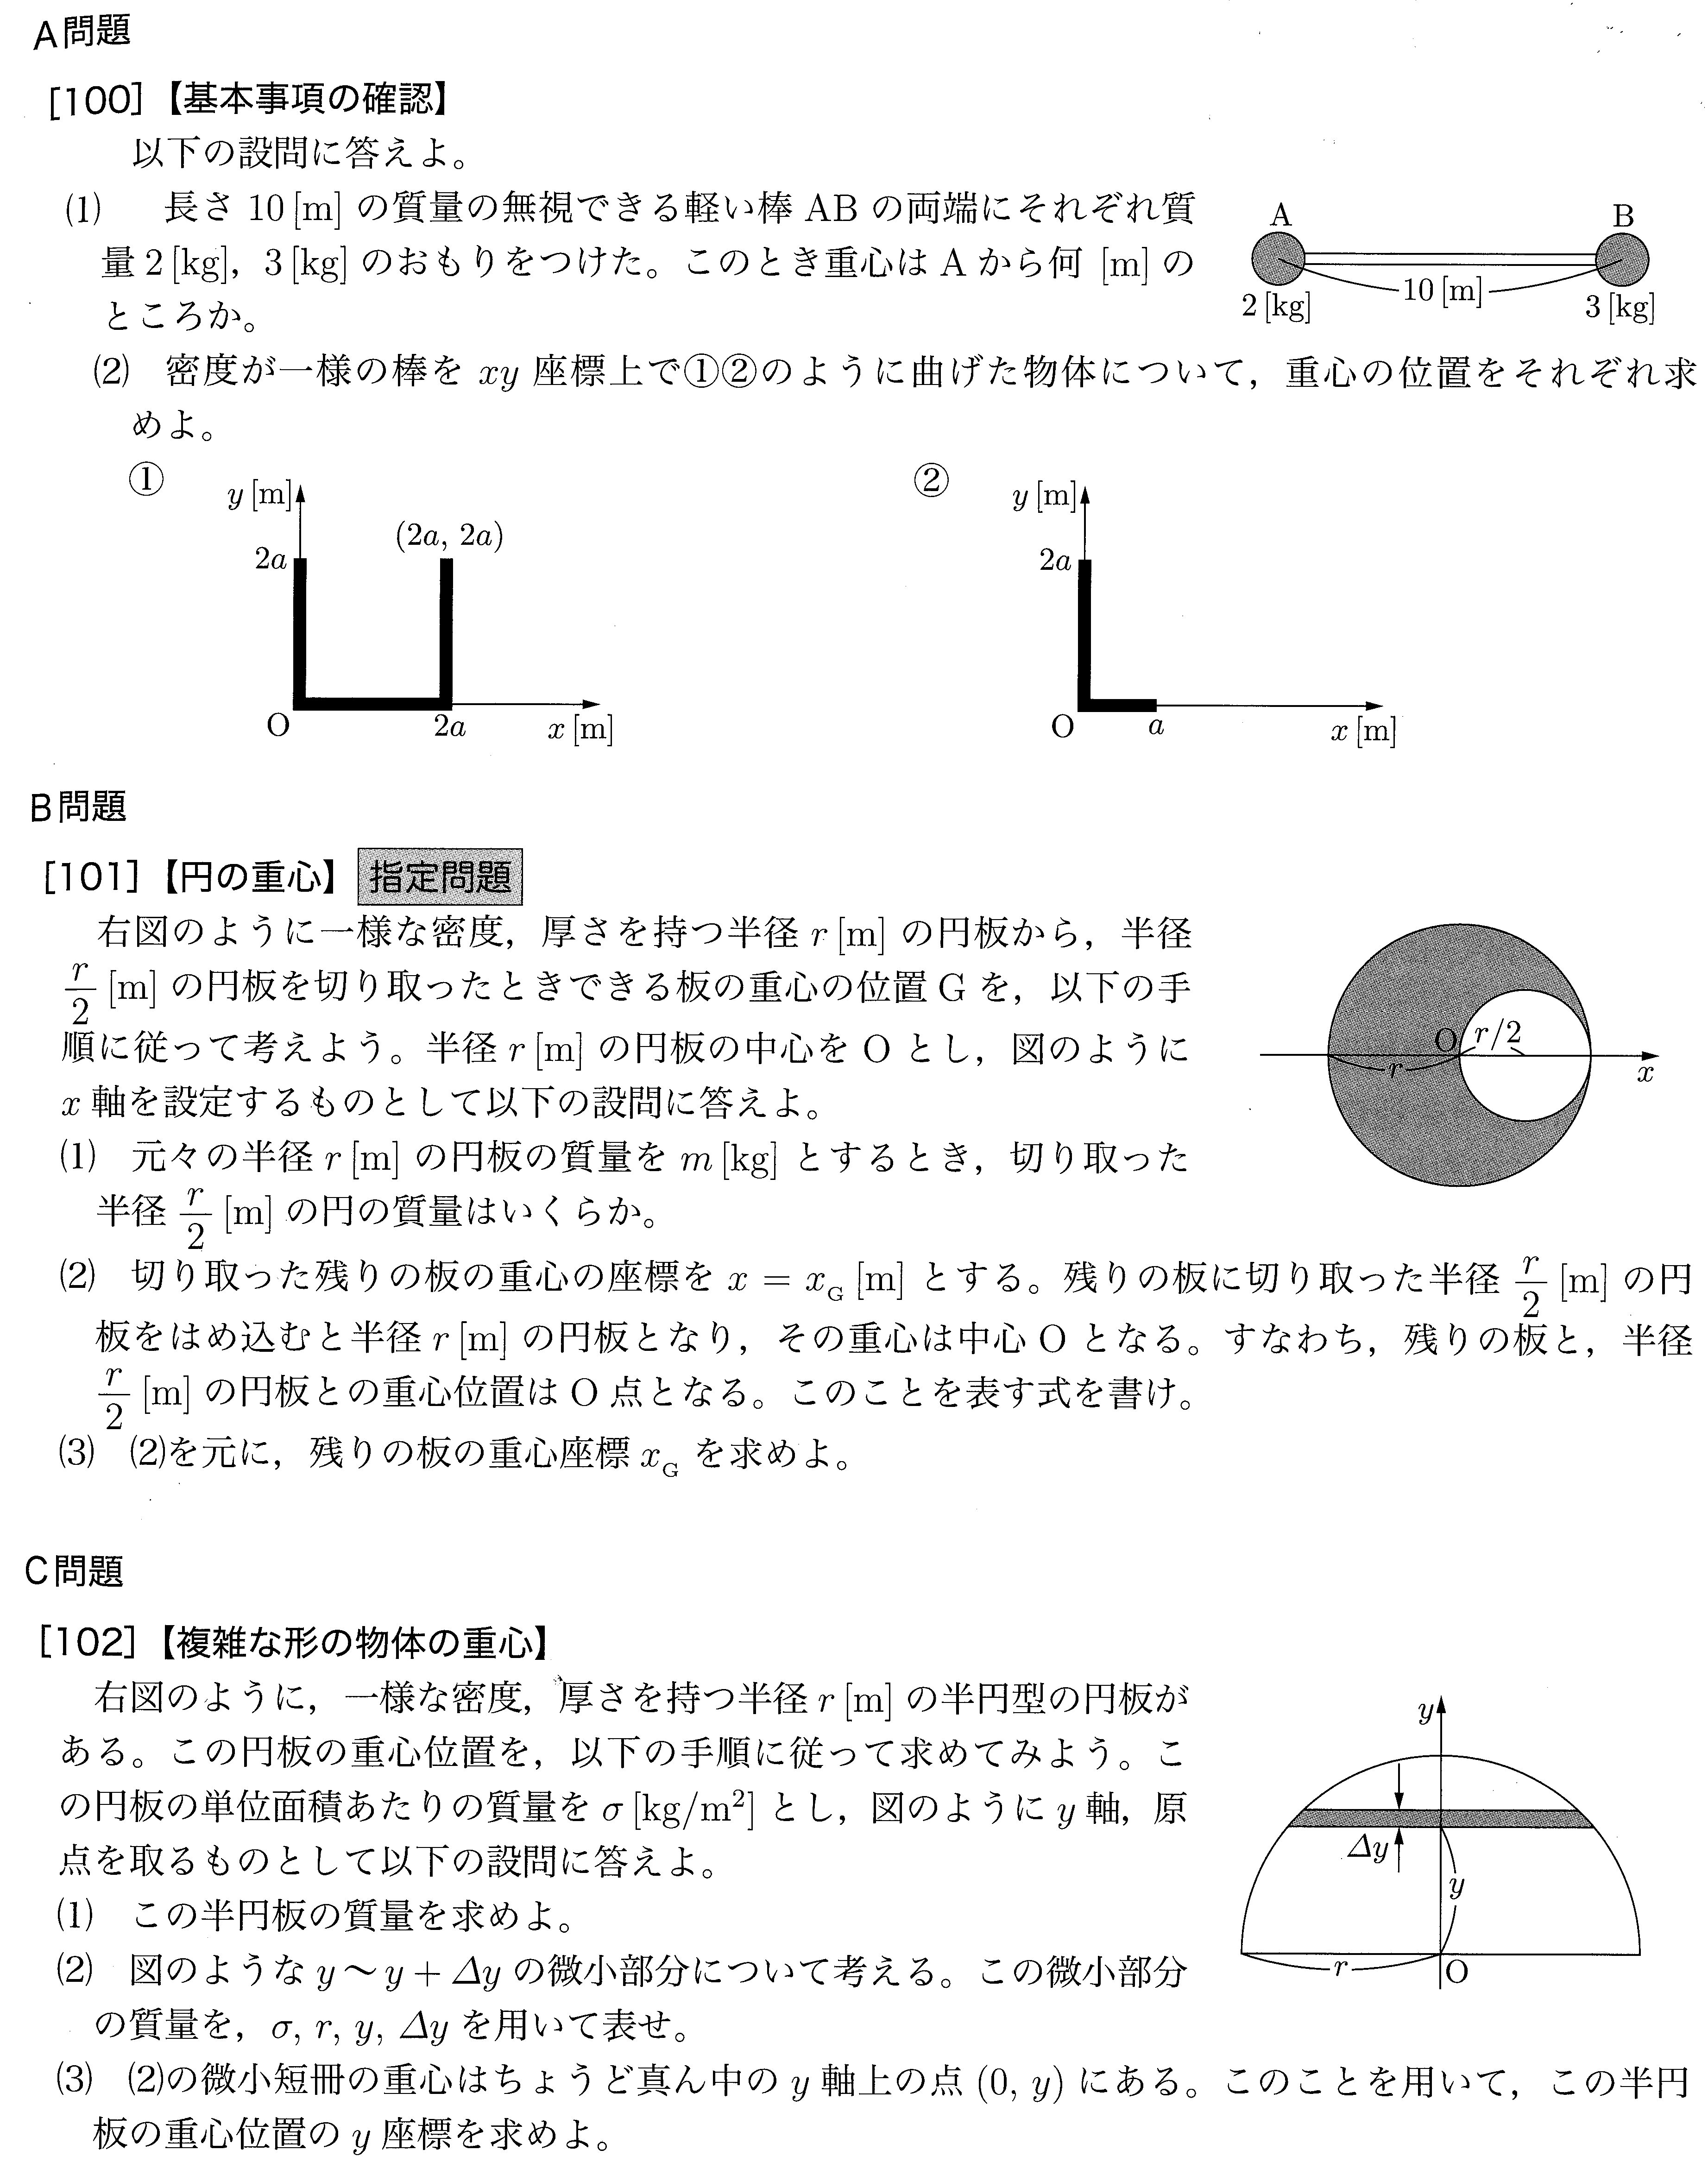
\includegraphics[width=170mm]{prob_p33.png}
\end{center}
\end{figure}

\newpage

\begin{figure}[h]
\begin{center}
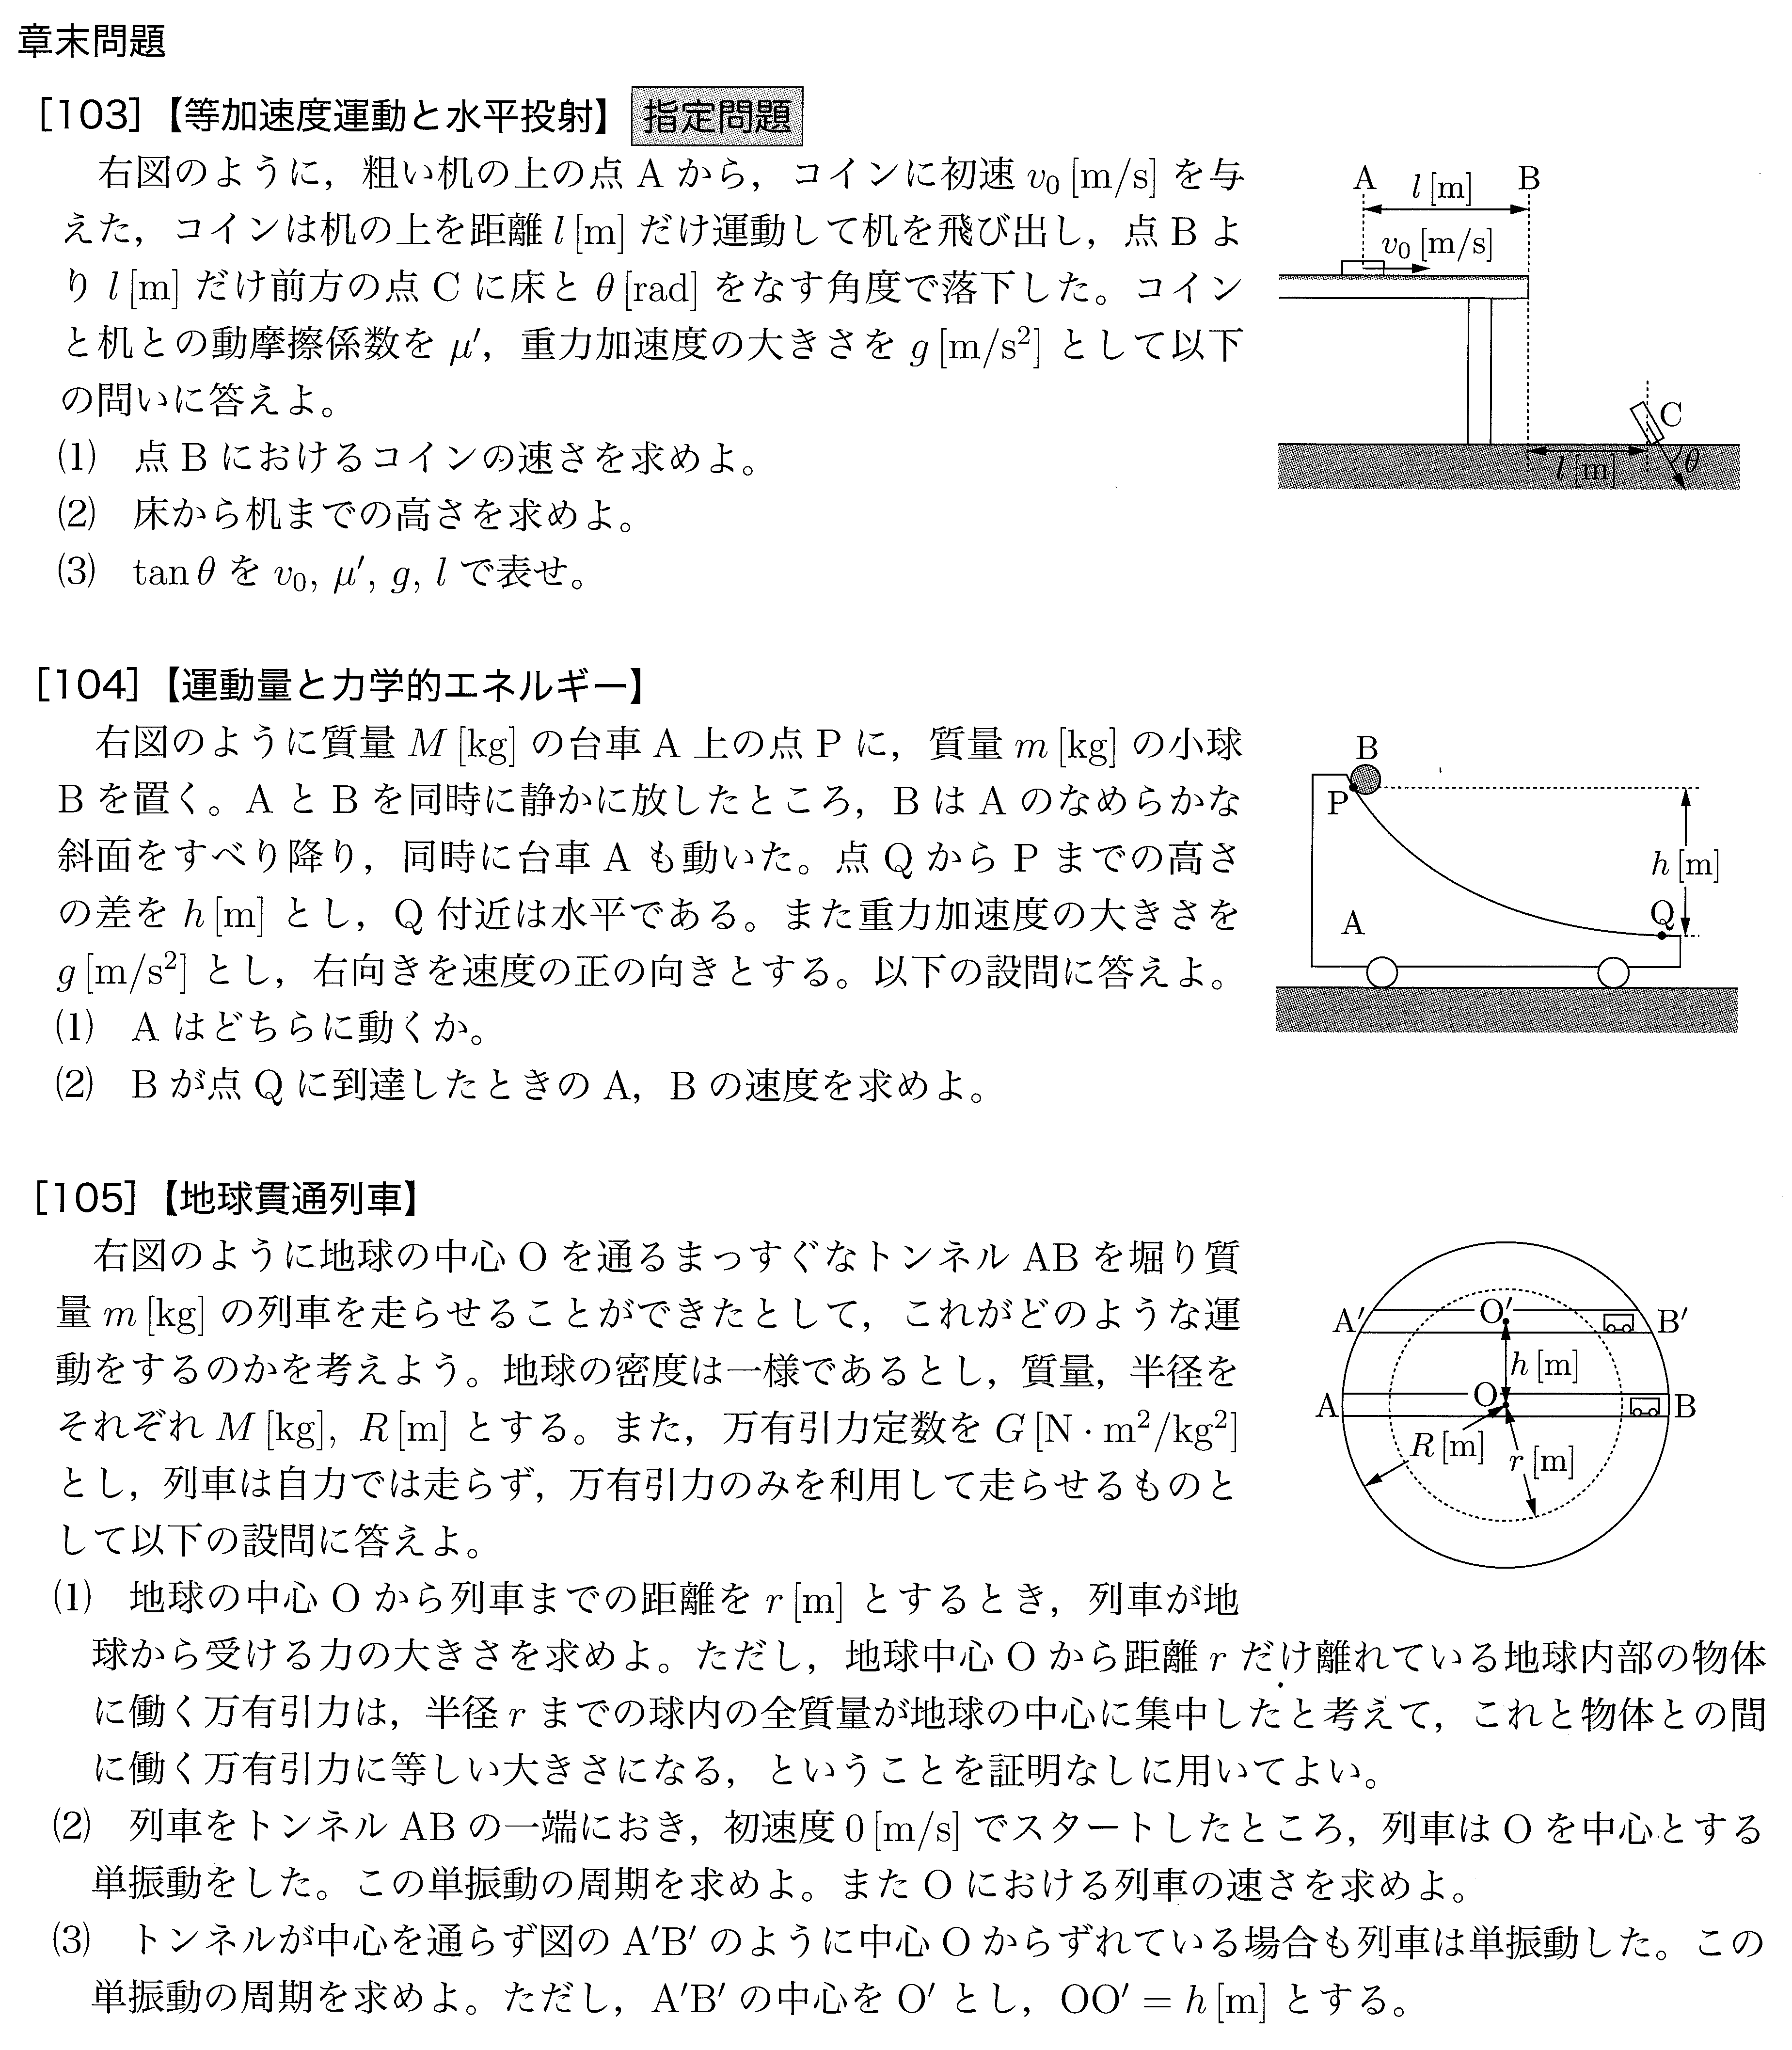
\includegraphics[width=170mm]{prob_p34.png}
\vspace{10cm}
\end{center}
\end{figure}



\newpage

\begin{figure}[h]
\begin{center}
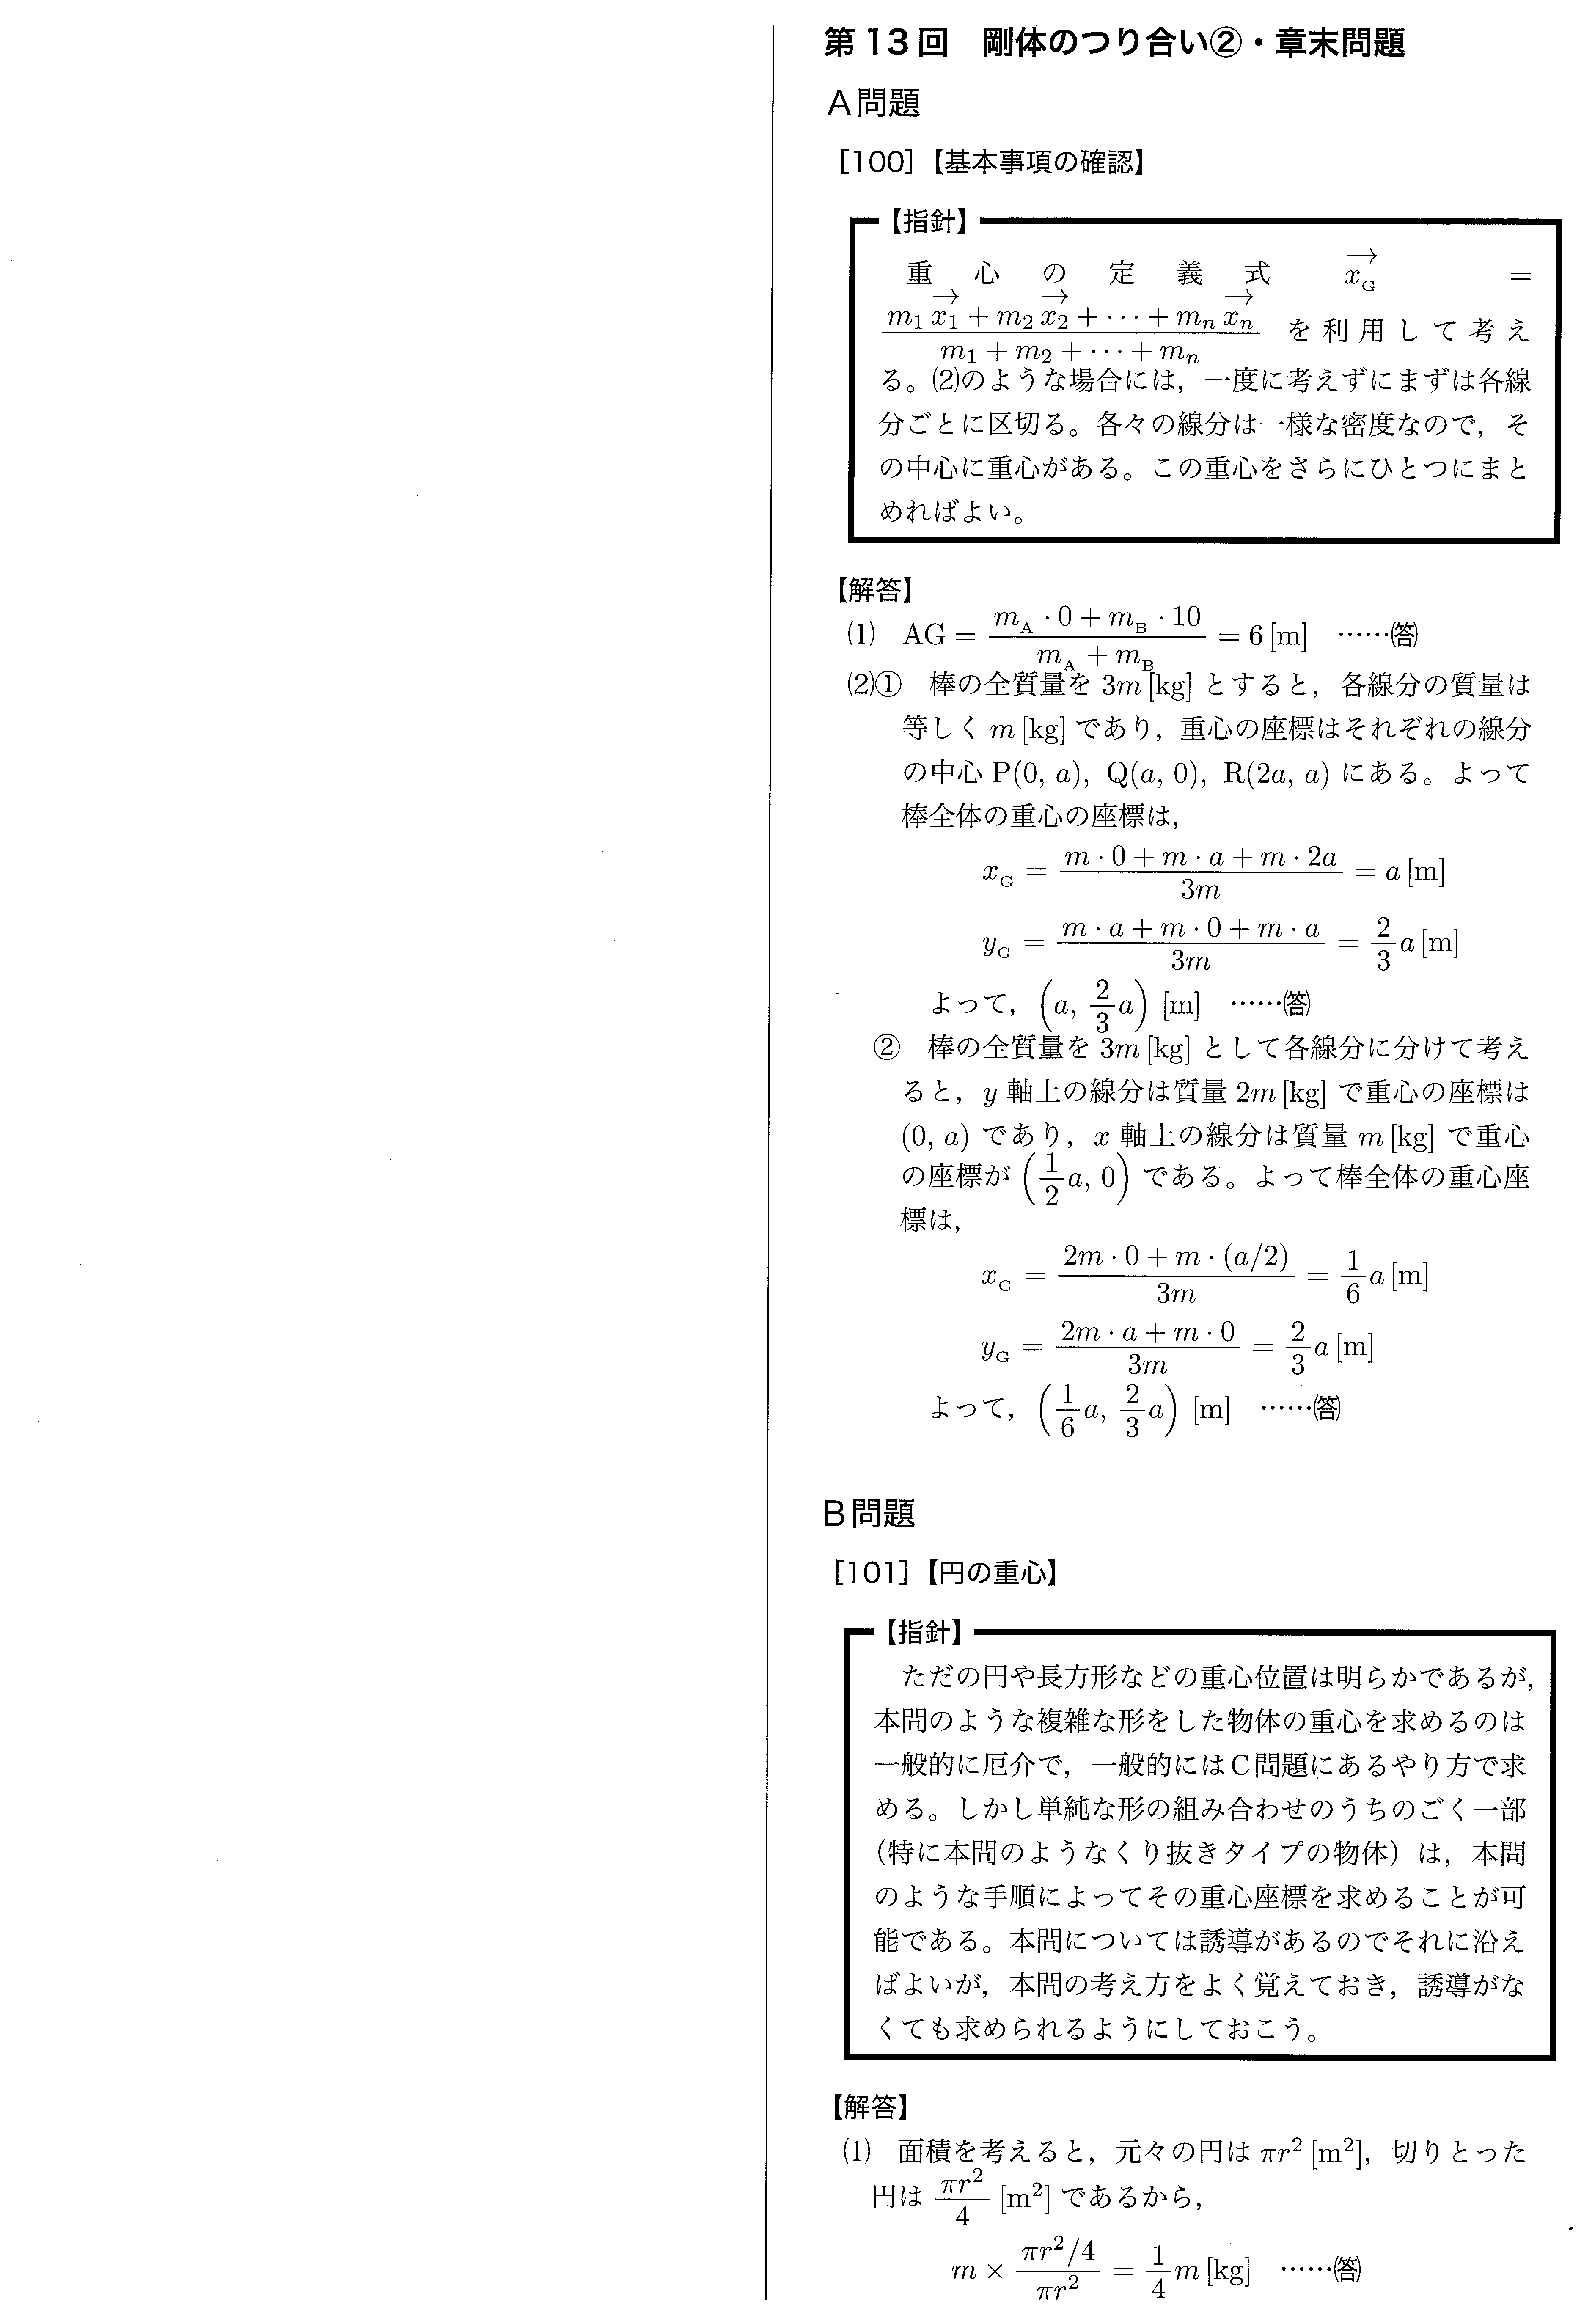
\includegraphics[width=170mm]{prob_p113_2.png}
\vspace{20cm}
\end{center}
\end{figure}

\newpage

\begin{figure}[h]
\begin{center}
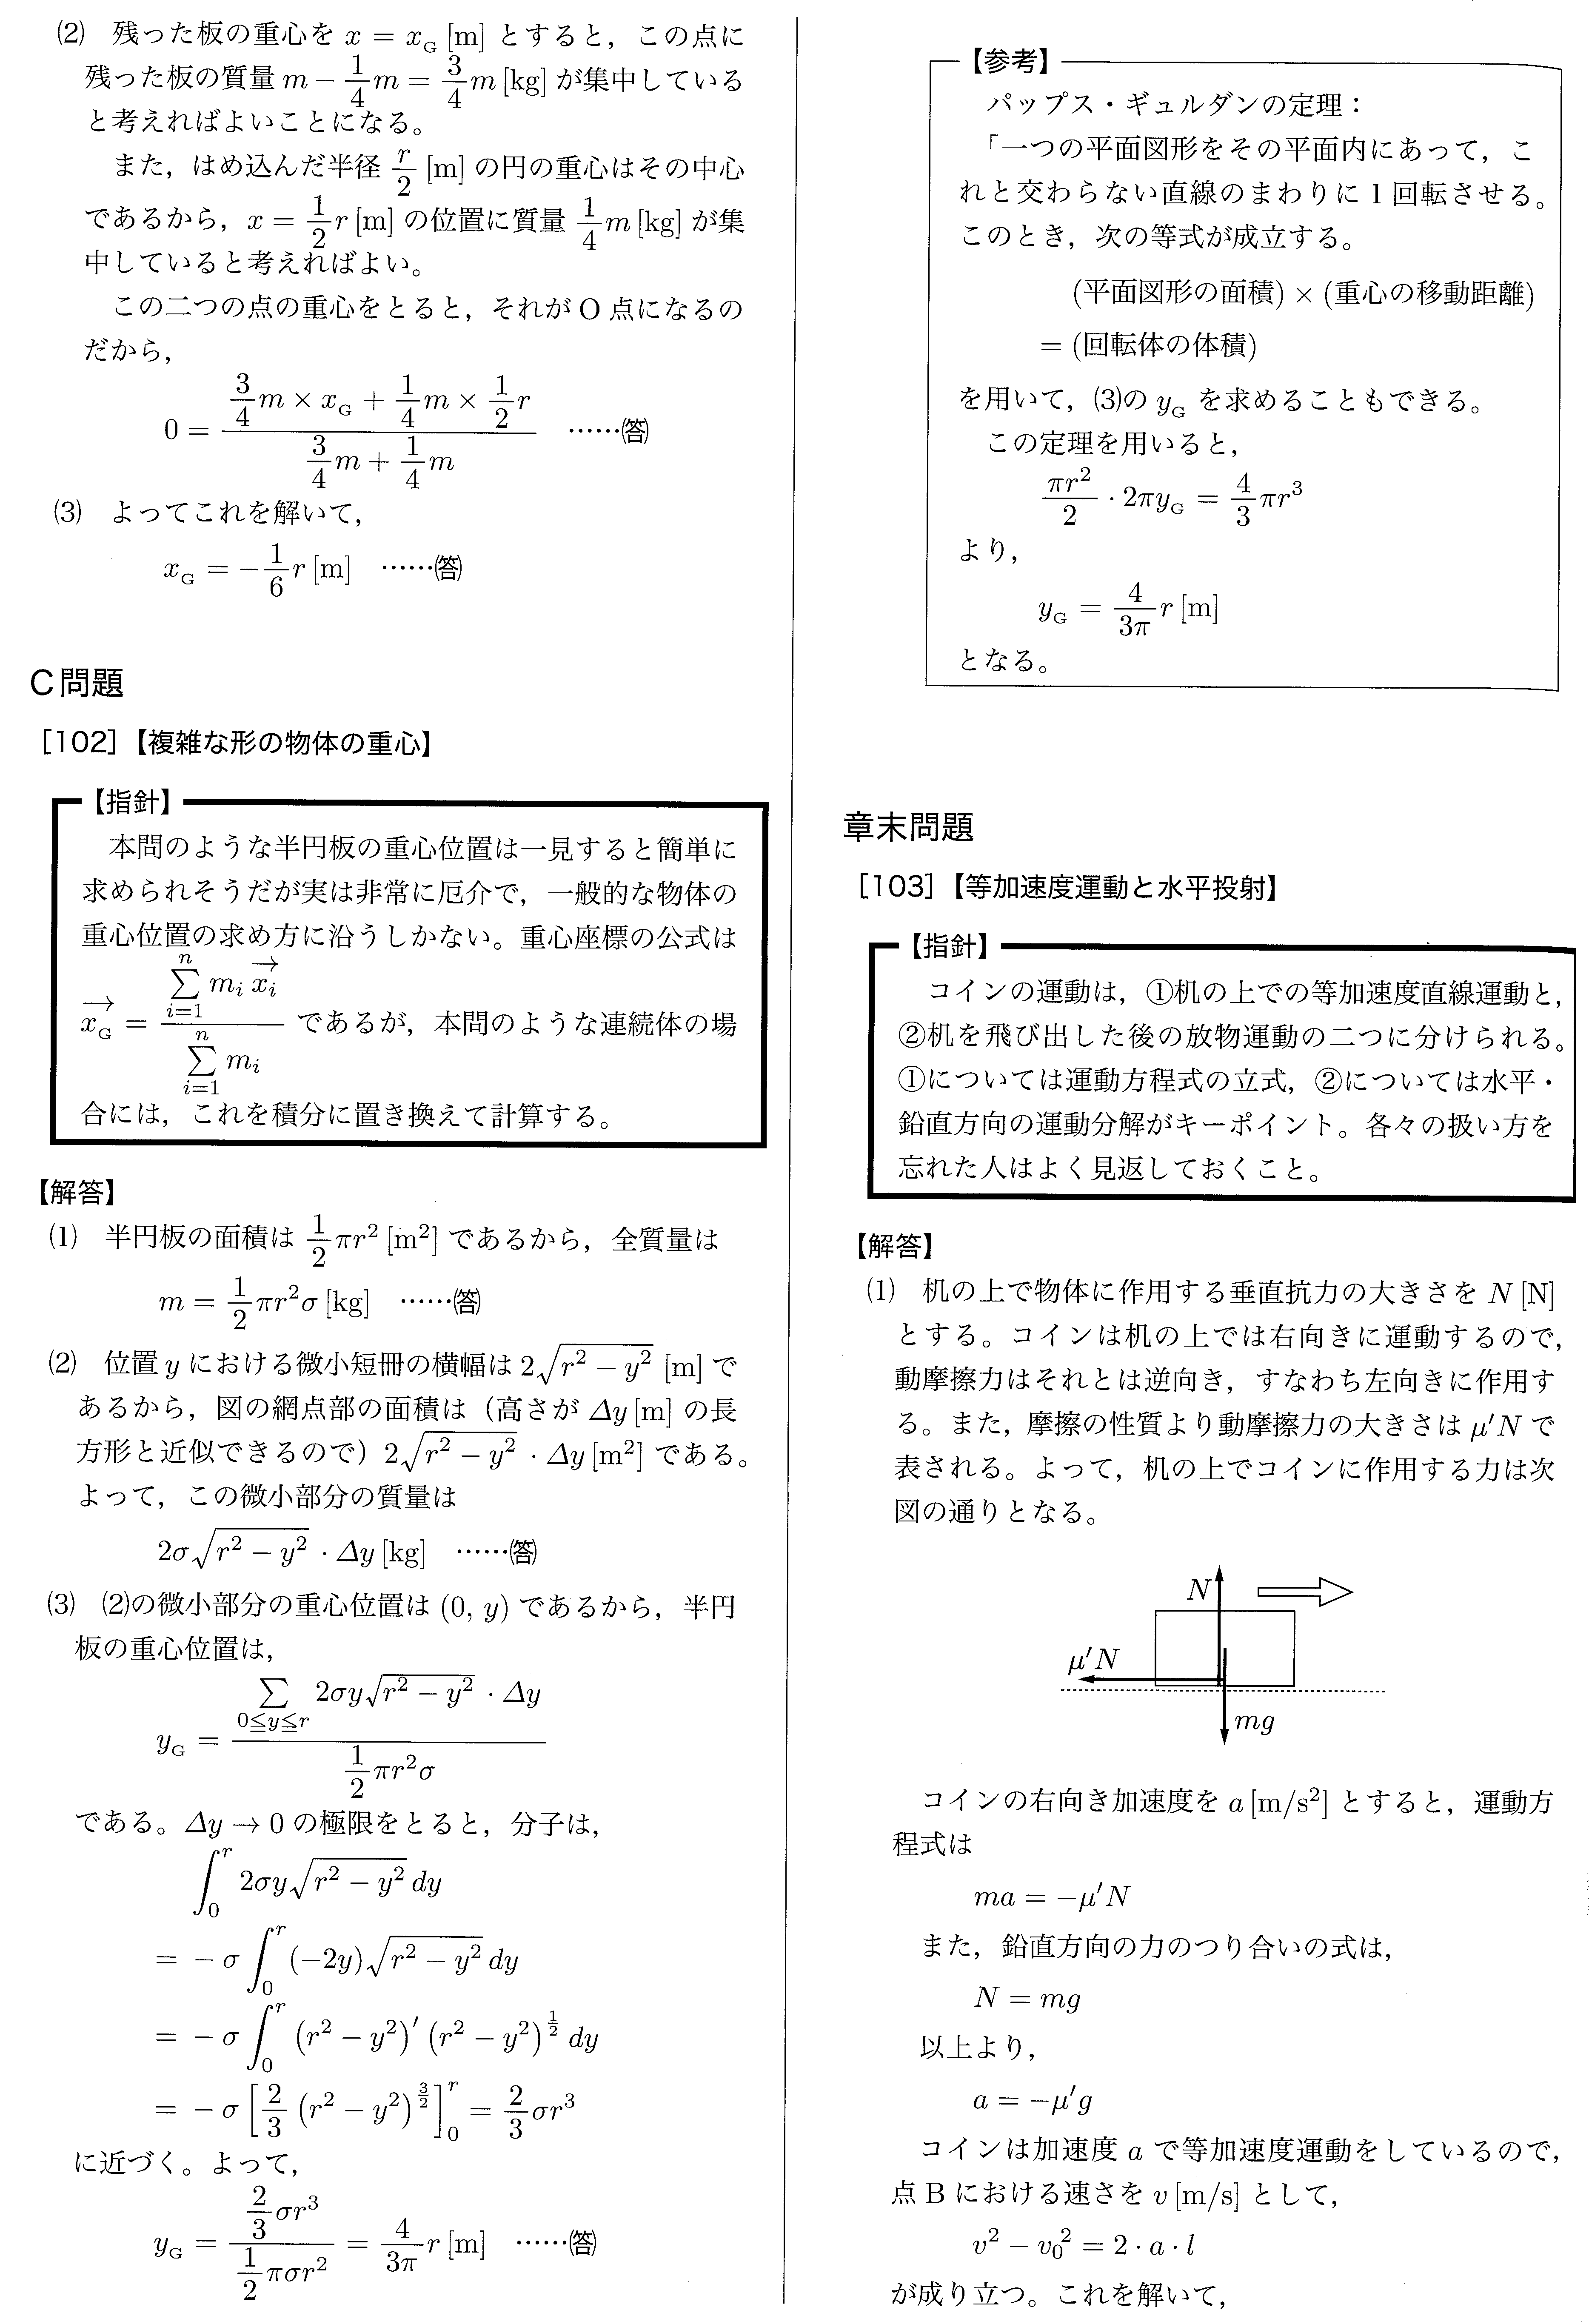
\includegraphics[width=170mm]{prob_p114.png}
\end{center}
\end{figure}

\newpage

\begin{figure}[h]
\begin{center}
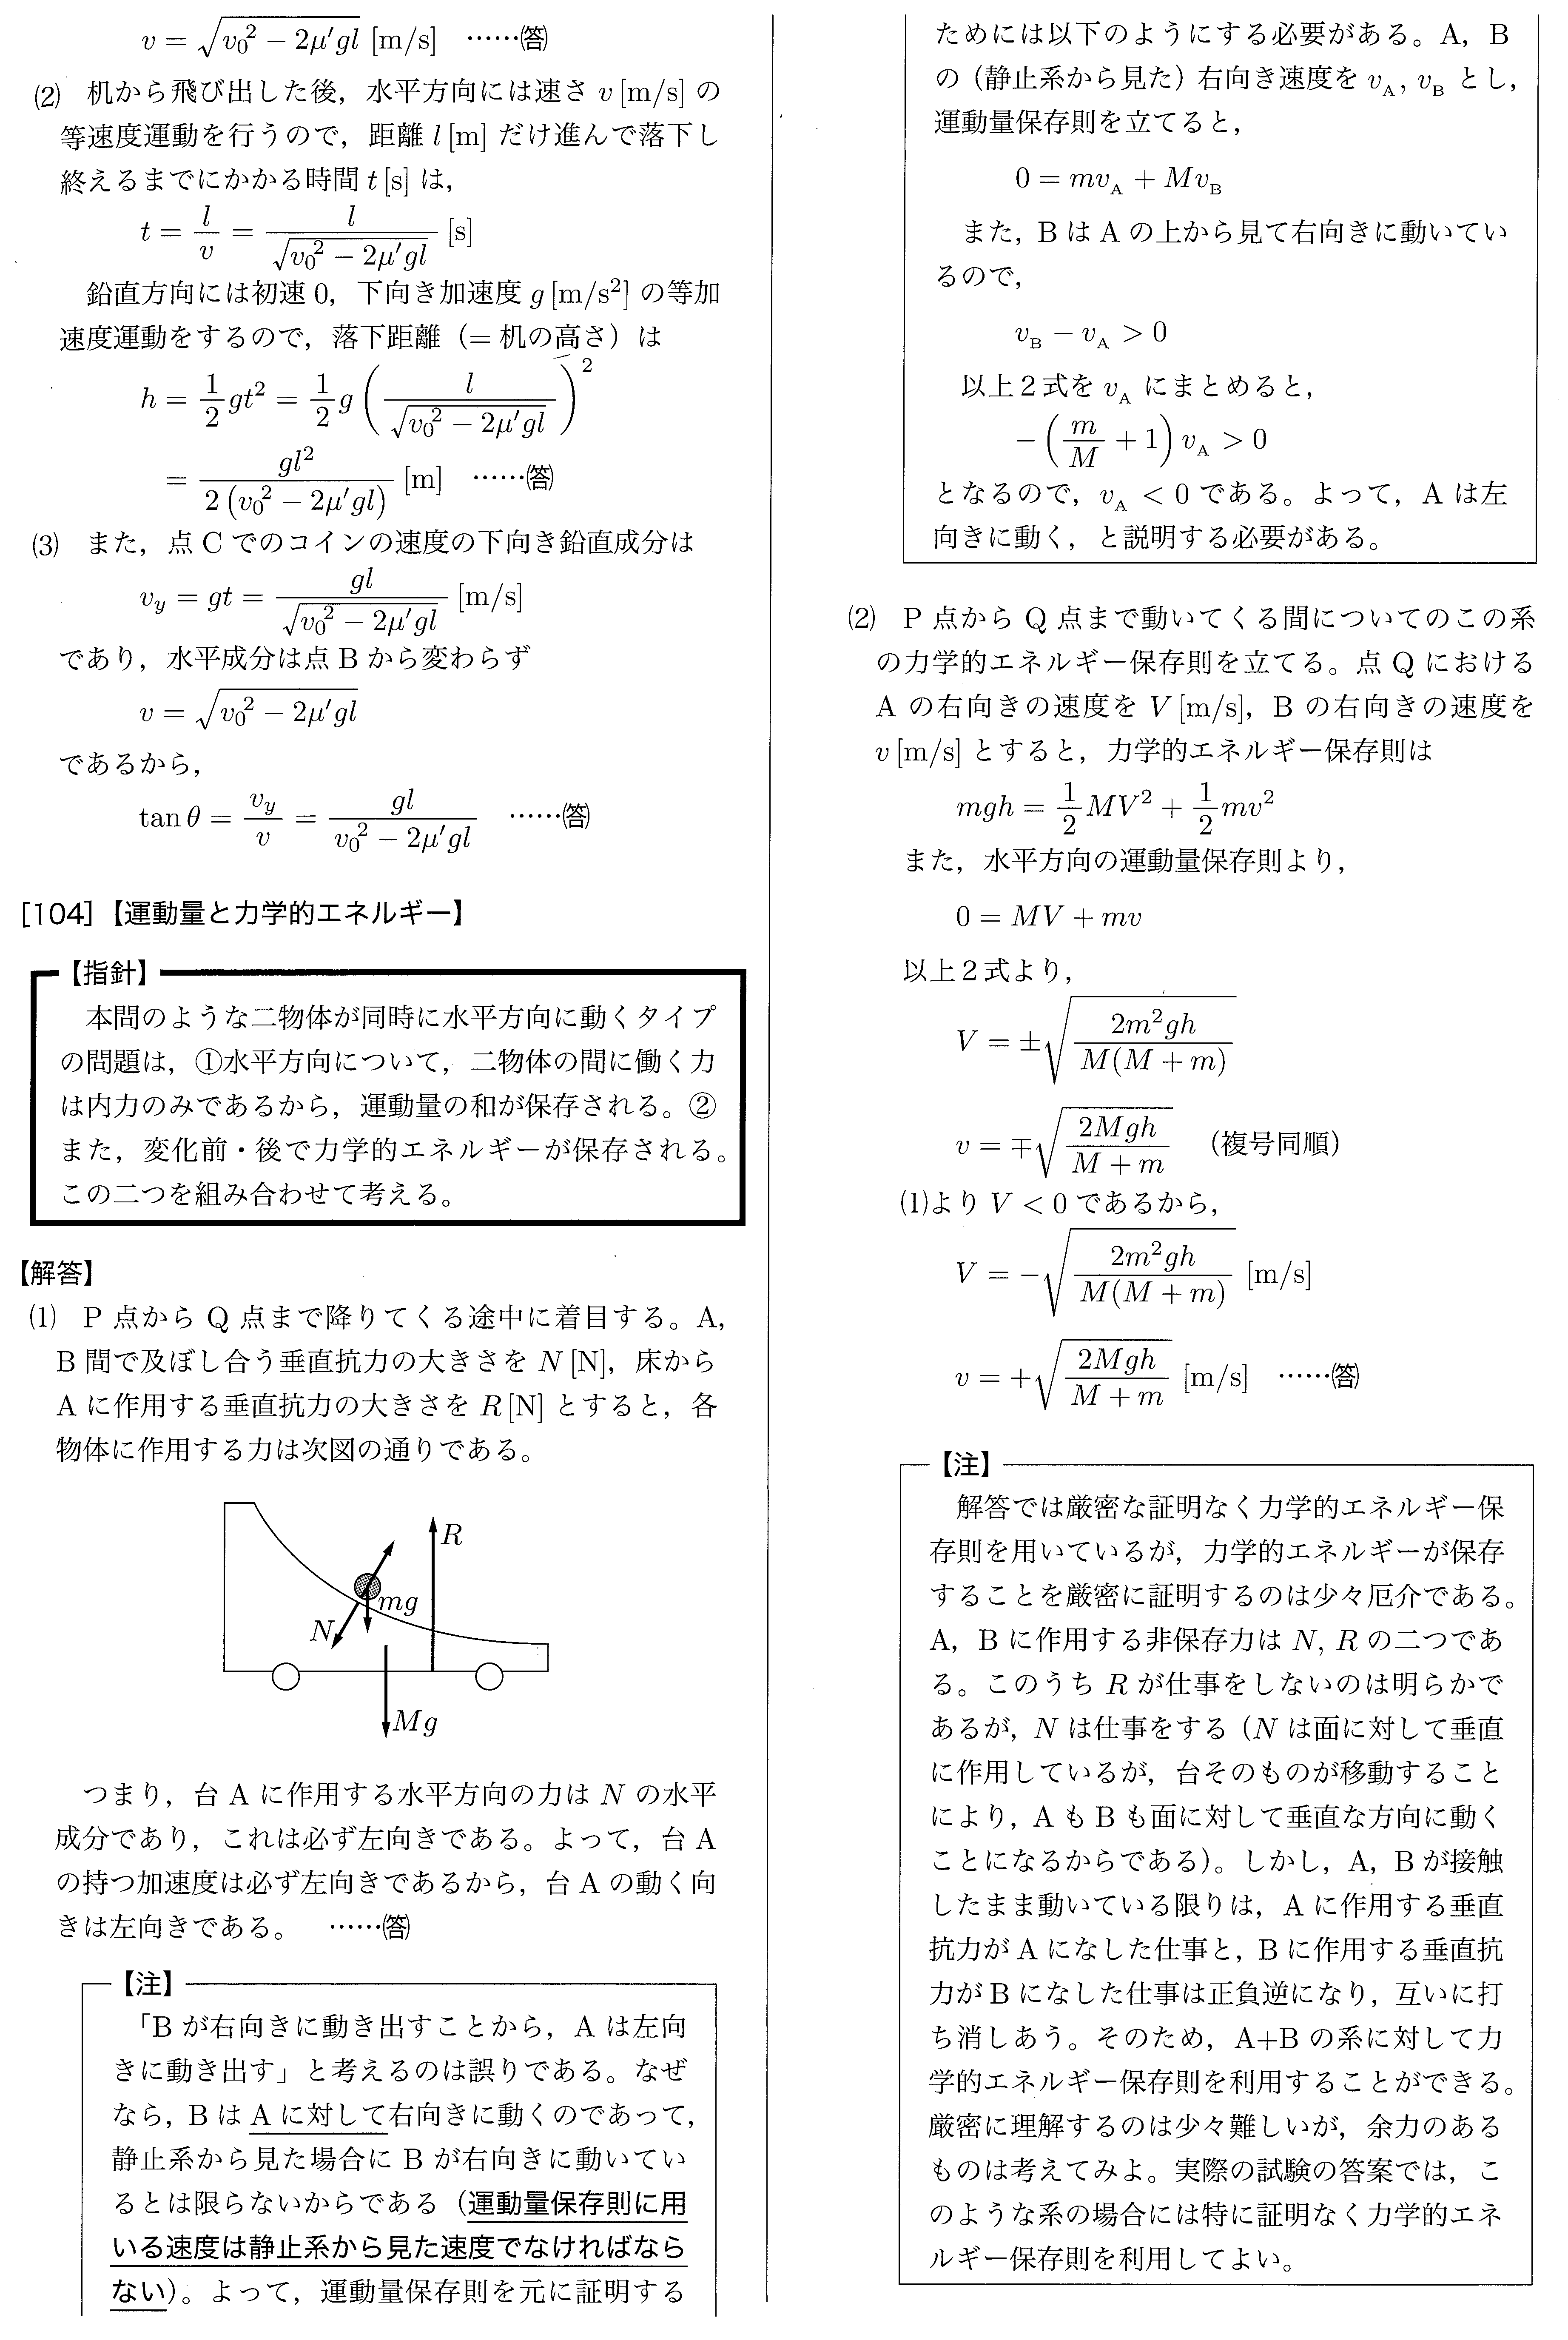
\includegraphics[width=170mm]{prob_p115.png}
\end{center}
\end{figure}
 
 \newpage

\begin{figure}[h]
\begin{center}
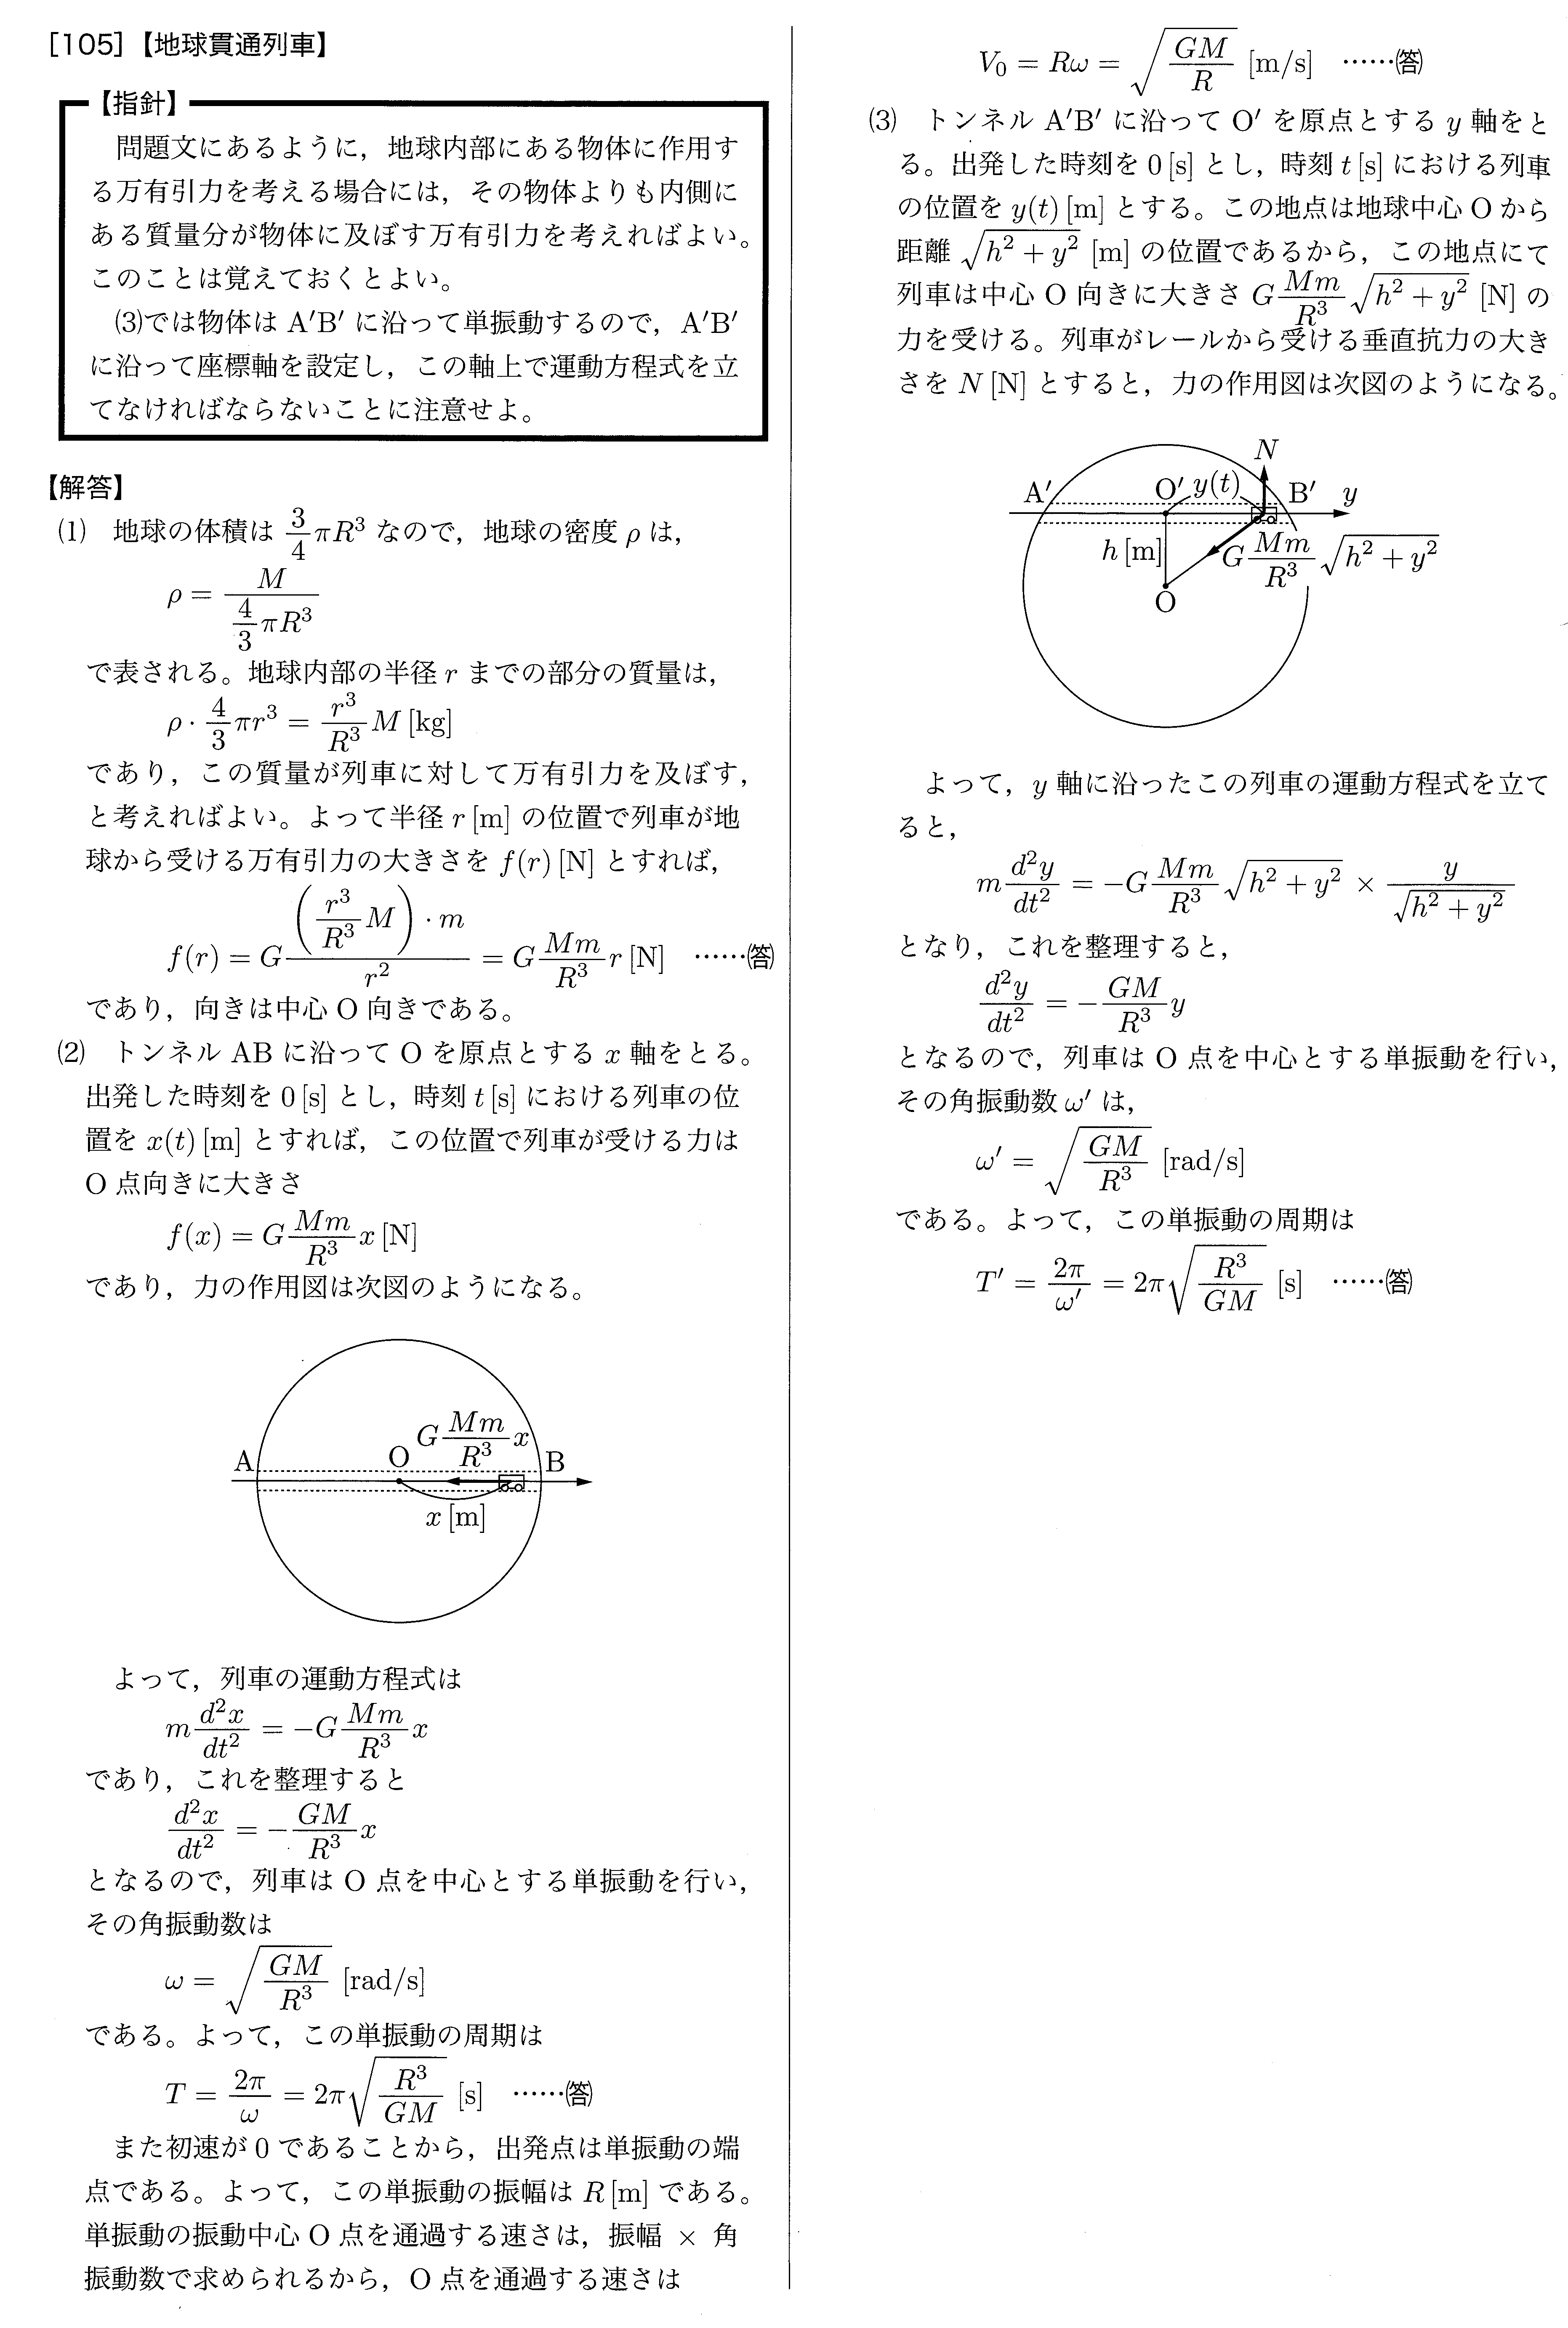
\includegraphics[width=170mm]{prob_p116.png}
\end{center}
\end{figure}

\begin{center}
{\Huge \bf 第2章　熱力学}
\end{center}

\section{気体の状態方程式・熱力学第一法則}

% 原本も第2章（熱力学）で例題番号を【例題1】に振り直しているので合わせる
\setcounter{nombre}{0}

\subsection{圧力・温度・モル}

気体を特徴づける物理量には圧力，体積，物質量，温度，分子量などがある．
まずこれらの定義をまとめる．\\
\begin{wrapfigure}[8]{r}[5mm]{70mm}
  \centering
  \vspace{-5mm}
  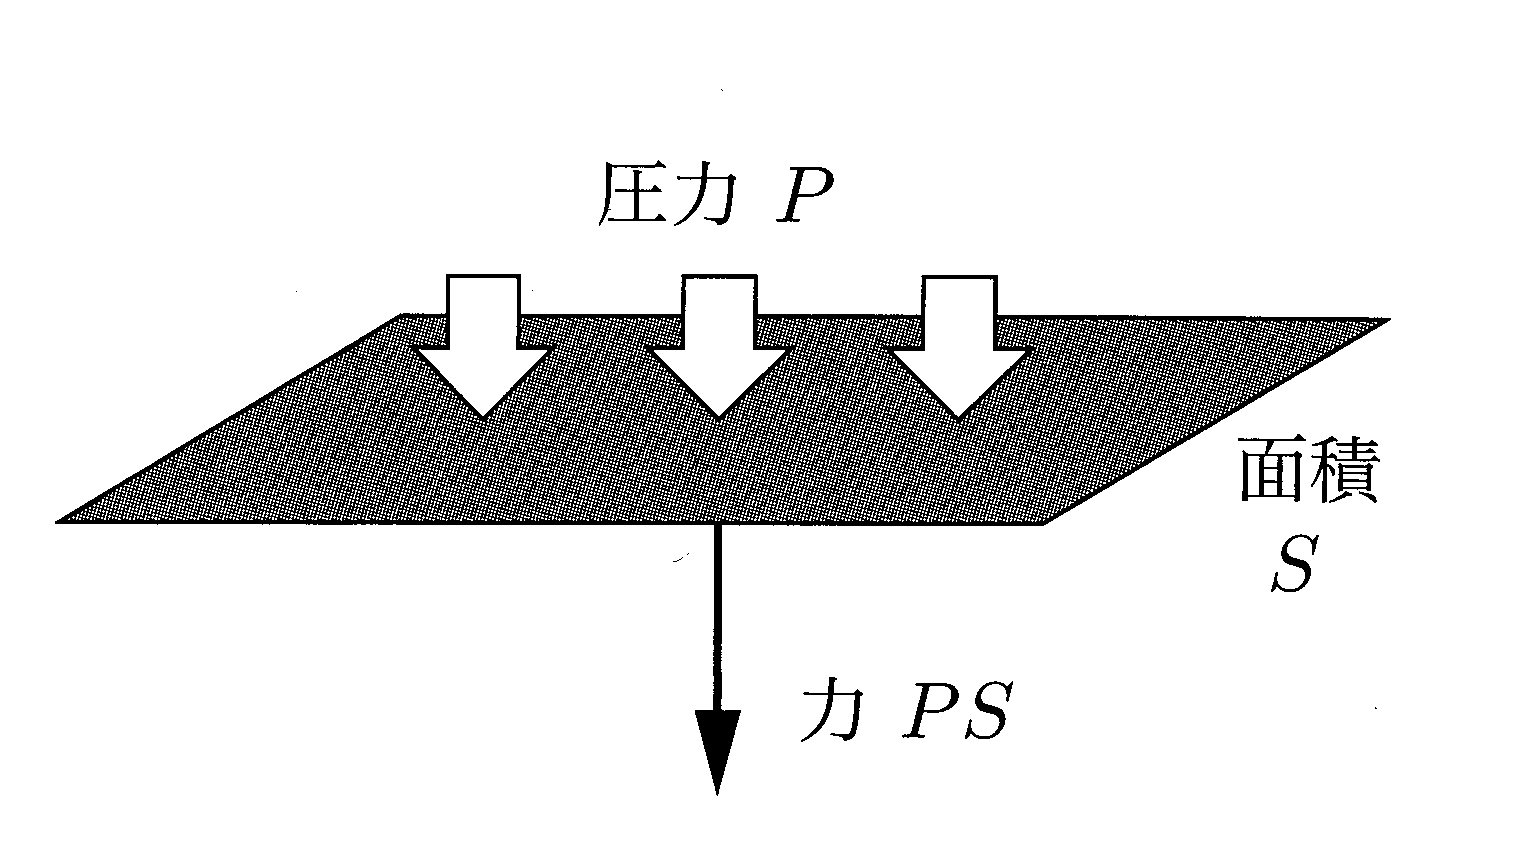
\includegraphics[keepaspectratio,width=70mm]
  {text_p63_fig1.png}
\end{wrapfigure}

\Kou{1}{圧力}

単位面積あたりに作用する力を圧力という．
面積$S\hspace{1mm}[{\rm m^2}]$の面に一様な圧力$P\hspace{1mm}$[Pa]が作用するとき，その面全体に作用する力$F$\hspace{1mm}[N]は
\[ \mbox{\boldmath  $F=PS$}\]
で与えられる．
圧力は面に対して垂直に作用し，気体の場合，その圧力は等方的で一様である．

物理では圧力の単位として{\bf [Pa]（パスカル）}を用いる．
圧力は{\bf ``単位面積あたりの力''}であるから，${\rm [N/m^2]}$を単位として用いることもある．
地表での大気圧は$10^5$[Pa]程度である．

容器に閉じ込められた気体の圧力は，その気体が押している面についての{\bf 力のつり合い}から決まる．
例えば断面積$S\hspace{1mm}[{\rm m^2}]$のシリンダーを質量$m$[kg]のピストンでふさいだ場合，ピストンにはたらく力は，下向きに大気からの力$P_0S$[N]と重力$mg$[N]，上向きに中の気体からの力$PS$[N]である．
ピストンが静止しているならこれらがつり合うので，
\[ PS=P_0S+mg \hspace{5mm}\mbox{すなわち}\hspace{5mm} P=P_0+\frac{mg}{S} \]
と，中の気体の圧力$P$[Pa]が求まる．
{\bf 気体の圧力を問われたら，まずその気体が押している面についての力のつり合いを考えればよい．}

同じ考え方で水中の圧力（{\bf 水圧}）も求められる．
密度$\rho\hspace{1mm}[{\rm kg/m^3}]$の水の中，深さ$h$[m]の位置にある断面積$S\hspace{1mm}[{\rm m^2}]$の水柱を考えると，この水柱にはたらく力は，上面を押す大気からの力$P_0S$[N]，水柱自身の重力$\rho hSg$[N]，そして下面を押し上げる力$p(h)S$[N]である．
水柱は静止しているのでこれらがつり合い，
\[ p(h)S=P_0S+\rho hSg \hspace{5mm}\mbox{すなわち}\hspace{5mm} p(h)=P_0+\rho gh \]
となる．水圧は深さに比例して大きくなる．\\

\Kou{2}{物質量（モル数）}

気体は分子から構成されているが，分子の個数は非常に多いため，個数を単位とするのは面倒である．
そこで，$6.02\times 10^{23}$個をひと束として扱い，これを{\bf 1[mol]（モル）}と呼ぶ．
気体の量を表す際には質量を用いるよりも，この物質量を用いることの方が多い．
$6.02\times 10^{23}$を{\bf アボガドロ数} \mbox{\boldmath $N_A$}と呼ぶ．
炭素の同位体の一つ$^{12}{\rm C}$の12[g]中に含まれる炭素原子の数として定義されている．\\

\Kou{3}{温度（絶対温度）}

我々が通常用いている温度単位は$\Cel$であるが，これを{\bf セルシウス温度}という．
セルシウス温度は氷の融点を0$\Cel$，水の沸点を100$\Cel$としてその間を100等分するように定義された温度単位であるが，気体の温度を表す際には{\bf 絶対温度[K]（ケルビン）}を用いる．
絶対温度$T$[K]はセルシウス温度$t$$\Cel$を273.15度だけずらしたもので，
\[T=t+273.15\]
の関係を持つ．\\

\Kou{4}{分子量}

分子1[mol] あたりの質量をグラム単位で表示したもののことを{\bf 分子量}という．
厳密には，分子量は分子1[mol]あたりの質量を$^{12}{\rm C}$の1[mol]あたりの質量を12として測った比の値として定義されるため定義上は単位を持たないが，実際には[g/mol]の単位を持つと解釈して考えてしまってよい．\\

\begin{matome}{圧力・物質量・温度・分子量}
 \hspace{3mm} 圧力$P$[Pa]\hspace{14mm} 単位面積あたりの力で，$F=PS$が成立．\\
\hspace{3mm} 物質量$n$[mol]\hspace{10mm} 分子数$N=nN_A$\hspace{10mm} アボガドロ数$N_A$\\
\hspace{3mm} 絶対温度$T$[K]\hspace{10mm} $T=$セルシウス温度$t\Cel+273.15$\\
\hspace{4mm}分子量$M$\hspace{16mm} 分子1[mol]あたりの質量\\
\hspace{3mm} 気体の圧力\hspace{11mm} その気体が押している面の力のつり合いから決まる
\end{matome}

\begin{reidaiunit}
\begin{reidai}{気体に関する各量}
\begin{zuright}{42mm}
\hspace{1zw}気体などに関する以下の各設問に答えよ．ただし重力加速度の大きさを$g\U{m/s^2}$，アボガドロ数を$N_{\mathrm{A}}=6.02\times 10^{23}$，窒素の分子量を28とする．
\begin{komon}
\ko{1} 断面積が$S\U{m^2}$のシリンダーに質量$m\U{kg}$のピストンを入れ，中に気体を封入したところ，ピストンは図の位置で静止した．大気圧を$P_0\U{Pa}$とすると，このとき封入されている気体の圧力はどれだけか．また，シリンダーの底面が気体から受ける力を求めよ．
\ko{2} 窒素$\mathrm{N_2}$気体$56\U{g}$中に含まれる窒素分子の数を求めよ．
\ko{3} 窒素の沸点は$77\U{K}$である．これはセルシウス温度では何度に相当するか．
\ko{4} 水の密度を$\rho\U{kg/m^3}$，大気圧を$P_0\U{Pa}$とする．水深$h\U{m}$の位置における水圧$p(h)\U{Pa}$を右図の水柱の力のつり合いから求めよ．
\end{komon}
\zusep
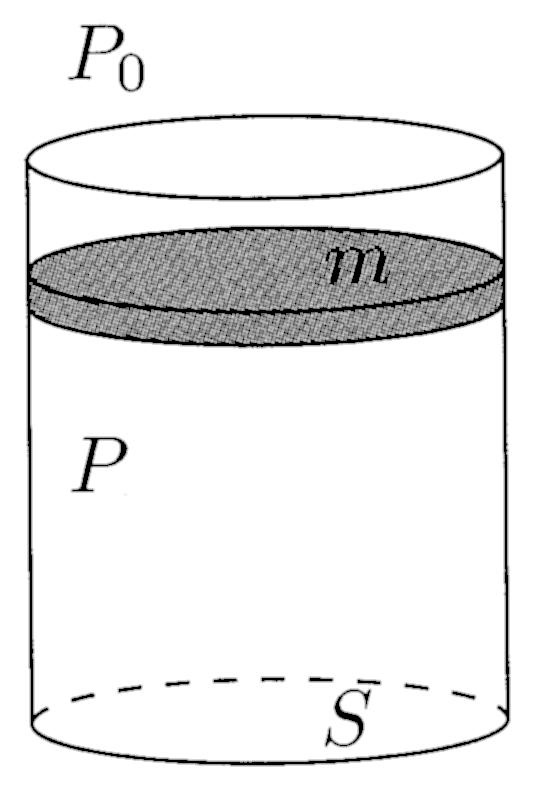
\includegraphics[keepaspectratio,width=26mm]{fig/ch14_ex1_cyl.png}\\[4mm]
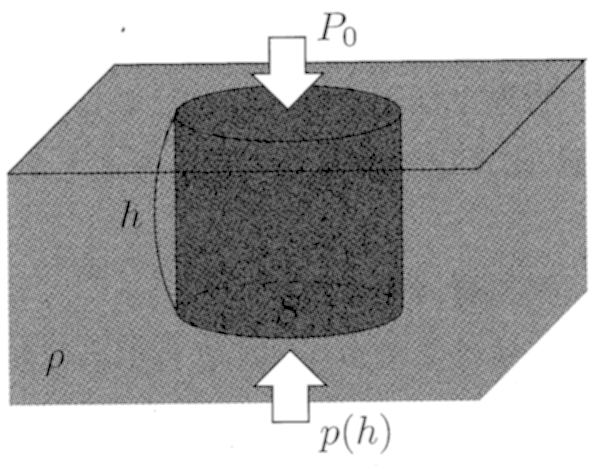
\includegraphics[keepaspectratio,width=42mm]{fig/ch14_ex1_water.png}
\end{zuright}
\end{reidai}

\begin{sisinE}
(1)は，ピストンにはたらく力のつり合いから中の気体の圧力を求める．気体の圧力を問われたら，その気体が押している面についての力のつり合いを考えるのであった．(4)も全く同じ考え方で，図の水柱についての力のつり合いを立てればよい．

(2)は分子量と物質量の関係，(3)は絶対温度とセルシウス温度の関係を使うだけである．
\end{sisinE}

\Key{$F=PS$\quad $N=nN_A$\quad $T=t+273.15$\quad 分子量$M$}

\begin{kaitou}
\begin{komon}
\ko{1} ピストンにはたらく力のつり合いより，
       \[PS=P_0S+mg\]
       よって，封入されている気体の圧力は，
       \[P=P_0+\frac{mg}{S}\U{Pa}\Ans\]
       また，シリンダーの底面が気体から受ける力は，$F=PS$より，
       \Ana{F=P_0S+mg\U{N}\Ans}
\ko{2} 窒素の分子量が28であるから，$\mathrm{N_2}$は1[mol]あたり$28\U{g}$である．よって$56\U{g}$の物質量は，
       \[n=\frac{56}{28}=2.0\U{mol}\]
       したがって分子数は，
       \Ana{\begin{aligned}
         N&=nN_{\mathrm{A}}=2.0\times 6.02\times 10^{23}\\
          &\fallingdotseq 1.2\times 10^{24}\,\text{[個]}\Ans
       \end{aligned}}
\ko{3} $T=t+273.15$より，
       \Ana{t=77-273.15=-196.15\fallingdotseq -196\Cel\Ans}
\ko{4} 図の水柱（断面積$S\U{m^2}$，高さ$h\U{m}$）にはたらく力は，上面を押す大気からの力$P_0S\U{N}$，水柱自身の重力$\rho hSg\U{N}$，下面を押し上げる力$p(h)S\U{N}$である．水柱は静止しているのでこれらがつり合い，
       \[p(h)S=P_0S+\rho hSg\]
       よって，
       \Ana{p(h)=P_0+\rho gh\U{Pa}\Ans}
\end{komon}
\end{kaitou}
\end{reidaiunit}
 
\subsection{気体の状態方程式}

体積$V[{\rm m^3}]$の容器に$n$[mol]の気体が均一に拡散しているとき，この気体の圧力を$P$[Pa]，気体の絶対温度を$T$[K]とすると，
\[\mbox{\boldmath $PV=nRT$}\]
という関係が，気体の種類によらず成立することが知られている．
これを{\bf 状態方程式}といい，比例定数$R[{\rm J/mol・K}]$を{\bf 気体定数}という．
実験により，気体定数の値は次の値をとることが知られている．
\[R=8.314[{\rm J/mol・K}] \]

この状態方程式は実在する気体全てについてほぼ成立するが，厳密には当てはまらないことが知られている．
実際にの気体は体積を持つこと，また気体分子間に相互作用（引力）が働くことが主な原因である．
この状態方程式が厳密に成立する気体を{\bf 理想気体}と呼ぶ．
理想気体であるための条件は，
\[ \MARU{1} 気体分子の体積が0[{\rm m^3}]である\]
\[ \MARU{2} 気体分子同士の相互作用がない\]
の2つである．
精密さを要求されない場合はこの状態方程式を用いてよい．
実在気体の場合でも，低圧，高温になると理想気体に近づく．

状態方程式を使う問題では，{\bf 変化の前と後のそれぞれについて状態方程式を立て，2式を組み合わせて未知の量を消去する}のが基本である．
このとき，変化の前後で値の変わらない量（物質量$n$や気体定数$R$，一定に保たれている圧力・体積・温度）を式の同じ側にまとめておくと計算が楽になる．
例えば温度が一定に保たれる変化なら$PV=nRT=$（一定）であるから，$PV$の値が変化しないことがすぐに分かる．

また，二つの容器が細い管でつながれている場合には，次の2点に注意する．
\[ \MARU{1} 気体が流れていなければ，両方の容器の気体の圧力は等しい \]
\[ \MARU{2} 容器の間で気体が移動しても，全体の物質量は変わらない \]
\MARU{1}は，左右に圧力差があると気体が流れてしまうことによる．
\MARU{2}は物質量の保存であり，コックを開いたあとの圧力を求める際にはこの関係を用いる．
なお，つながれた二つの容器の{\bf 温度が等しいとは限らない}．
温度が違う場合は全体をひとまとめにできないので，容器ごとに状態方程式を立てて物質量の和を考える．

\begin{matome}{状態方程式}
 \hspace{3mm} $PV=nRT$\\
\hspace{3mm} 変化の前後で状態方程式を立てて組み合わせる\\
\hspace{3mm} つながれた容器\hspace{5mm} 圧力は等しい／全体の物質量は保存する
\end{matome}

\begin{reidaiunit}
\begin{reidai}{状態方程式}
\begin{zuright}{42mm}
\hspace{1zw}容積$V_{\mathrm{A}}$, $V_{\mathrm{B}}\U{m^3}$の容器$\mathrm{A}$，$\mathrm{B}$が，図のようにコックを持つ細い管でつながっている．最初コックは閉じられており，温度$T\U{K}$の理想気体を$\mathrm{A}$，$\mathrm{B}$それぞれに圧力が$P_{\mathrm{A}}$, $P_{\mathrm{B}}\U{Pa}$となるだけ封入した．細管の部分の体積および容器の熱膨張は無視し，気体定数を$R\U{J/mol\cdot K}$として以下の問に答えよ．
\begin{komon}
\ko{1} $\mathrm{A}$，$\mathrm{B}$それぞれの中に含まれる理想気体の物質量$n_{\mathrm{A}}$, $n_{\mathrm{B}}\U{mol}$をそれぞれ求めよ．
\ko{2} 次に，温度を$T\U{K}$に保ったままコックを開いた．このときの容器内の圧力$P\U{Pa}$を求めよ．
\ko{3} (2)において，$\mathrm{A}$から$\mathrm{B}$へ移動した理想気体の物質量$\Delta n\U{mol}$を求めよ．
\ko{4} コックを開いたままの状態で，$\mathrm{A}$の温度を$T_{\mathrm{A}}\U{K}$，$\mathrm{B}$の温度を$T_{\mathrm{B}}\U{K}$に保った．このときの容器の圧力$P'\U{Pa}$を求めよ．
\end{komon}
\zusep
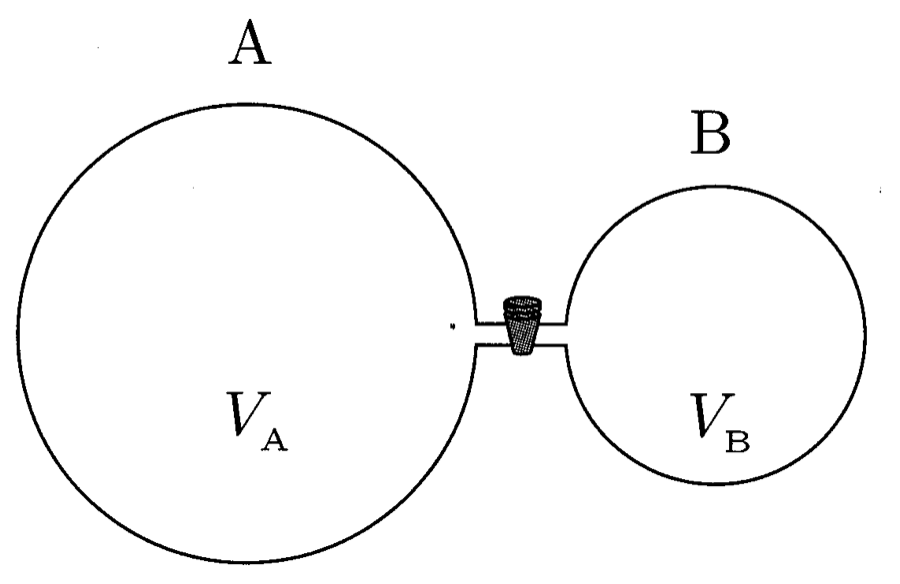
\includegraphics[keepaspectratio,width=42mm]{fig/ch14_ex2_cock.png}
\end{zuright}
\end{reidai}

\begin{sisinE}
コックを開く前と後のそれぞれについて状態方程式を立て，組み合わせればよい．コックを開いたあとは$\mathrm{A}$と$\mathrm{B}$の気体の圧力が等しくなること，そして$\mathrm{A}$，$\mathrm{B}$を合わせた全体の物質量が変わらないことがカギである．

(2)は$\mathrm{A}$と$\mathrm{B}$の温度が同じなので，$\mathrm{A}+\mathrm{B}$を体積$V_{\mathrm{A}}+V_{\mathrm{B}}$の一つの容器とみなしてよい．一方(4)では$\mathrm{A}$と$\mathrm{B}$の温度が違うのでひとまとめにできない．容器ごとに状態方程式を立て，物質量の和が変わらないことを使う．

左右に圧力差があると気体が流れる．すなわち{\bf 気体が流れていないとき左右の圧力は同じ}である．
\end{sisinE}

\Key{状態方程式\quad $PV=nRT$}


\begin{kaitou}
\begin{komon}
\ko{1} コックを開く前の$\mathrm{A}$，$\mathrm{B}$について状態方程式を立てると，
       \[\mathrm{A}:P_{\mathrm{A}}V_{\mathrm{A}}=n_{\mathrm{A}}RT\Eq{1}\]
       \[\mathrm{B}:P_{\mathrm{B}}V_{\mathrm{B}}=n_{\mathrm{B}}RT\Eq{2}\]
       よって，
       \Ana{n_{\mathrm{A}}=\frac{P_{\mathrm{A}}V_{\mathrm{A}}}{RT}\U{mol}, \quad n_{\mathrm{B}}=\frac{P_{\mathrm{B}}V_{\mathrm{B}}}{RT}\U{mol}\Ans}
\ko{2} コックを開くと$\mathrm{A}$と$\mathrm{B}$の気体の圧力は等しくなる．また，全体の物質量は$n_{\mathrm{A}}+n_{\mathrm{B}}$のまま変わらず，温度も$T$のままである．よって$\mathrm{A}+\mathrm{B}$を体積$V_{\mathrm{A}}+V_{\mathrm{B}}$の一つの容器とみなして状態方程式を立てると，
       \[P(V_{\mathrm{A}}+V_{\mathrm{B}})=(n_{\mathrm{A}}+n_{\mathrm{B}})RT\]
       \MARU{1}\MARU{2}を代入して，
       \Ana{P=\frac{P_{\mathrm{A}}V_{\mathrm{A}}+P_{\mathrm{B}}V_{\mathrm{B}}}{V_{\mathrm{A}}+V_{\mathrm{B}}}\U{Pa}\Ans\Eq{3}}
\ko{3} コックを開いた後の$\mathrm{A}$内の物質量を$n_{\mathrm{A}}'\U{mol}$とすると，$\mathrm{A}$についての状態方程式より，
       \[PV_{\mathrm{A}}=n_{\mathrm{A}}'RT\]
       $\mathrm{A}$から$\mathrm{B}$へ移動した物質量は$\Delta n=n_{\mathrm{A}}-n_{\mathrm{A}}'$であるから，\MARU{1}\MARU{3}より，
       \[\Delta n=\frac{(P_{\mathrm{A}}-P)V_{\mathrm{A}}}{RT}=\frac{V_{\mathrm{A}}V_{\mathrm{B}}(P_{\mathrm{A}}-P_{\mathrm{B}})}{RT(V_{\mathrm{A}}+V_{\mathrm{B}})}\U{mol}\]
       \hspace*{\fill}\Ans
\ko{4} $\mathrm{A}$と$\mathrm{B}$は細管でつながれているので圧力は等しく$P'\U{Pa}$である．一方，温度は$\mathrm{A}$が$T_{\mathrm{A}}$，$\mathrm{B}$が$T_{\mathrm{B}}$と異なるので，それぞれについて状態方程式を立てる．このときの$\mathrm{A}$，$\mathrm{B}$内の物質量を$n_{\mathrm{A}}''$, $n_{\mathrm{B}}''\U{mol}$とすると，
       \[\mathrm{A}:P'V_{\mathrm{A}}=n_{\mathrm{A}}''RT_{\mathrm{A}}\]
       \[\mathrm{B}:P'V_{\mathrm{B}}=n_{\mathrm{B}}''RT_{\mathrm{B}}\]
       \hspace{1zw}全体の物質量は変わらないので，
       \[n_{\mathrm{A}}''+n_{\mathrm{B}}''=n_{\mathrm{A}}+n_{\mathrm{B}}\]
       すなわち\MARU{1}\MARU{2}より，
       \[\frac{P'V_{\mathrm{A}}}{RT_{\mathrm{A}}}+\frac{P'V_{\mathrm{B}}}{RT_{\mathrm{B}}}=\frac{P_{\mathrm{A}}V_{\mathrm{A}}+P_{\mathrm{B}}V_{\mathrm{B}}}{RT}\]
       よって，
       \Ana{P'=\frac{(P_{\mathrm{A}}V_{\mathrm{A}}+P_{\mathrm{B}}V_{\mathrm{B}})T_{\mathrm{A}}T_{\mathrm{B}}}{T(V_{\mathrm{A}}T_{\mathrm{B}}+V_{\mathrm{B}}T_{\mathrm{A}})}\U{Pa}\Ans}
\end{komon}
\end{kaitou}
\end{reidaiunit}
 
\subsection{熱とエネルギー}

世の中にある物質は原子，分子によって構成されているが，熱は物質を構成している原子・分子の運動に基づく{\bf エネルギーの一つの形態}であり，熱いというのはその運動が激しい状態に対応し，冷たいというのは運動が少ない状態に対応している．
例えば，熱いものを触ったときに熱いと感じるのは，原子・分子が激しく運動してぶつかってくるのが原因である．
このように，熱や温度というのは物体の構成原子・分子の微細な運動と密接に関係している．

\begin{wrapfigure}[10]{r}[5mm]{70mm}
  \centering
  \vspace{-5mm}
  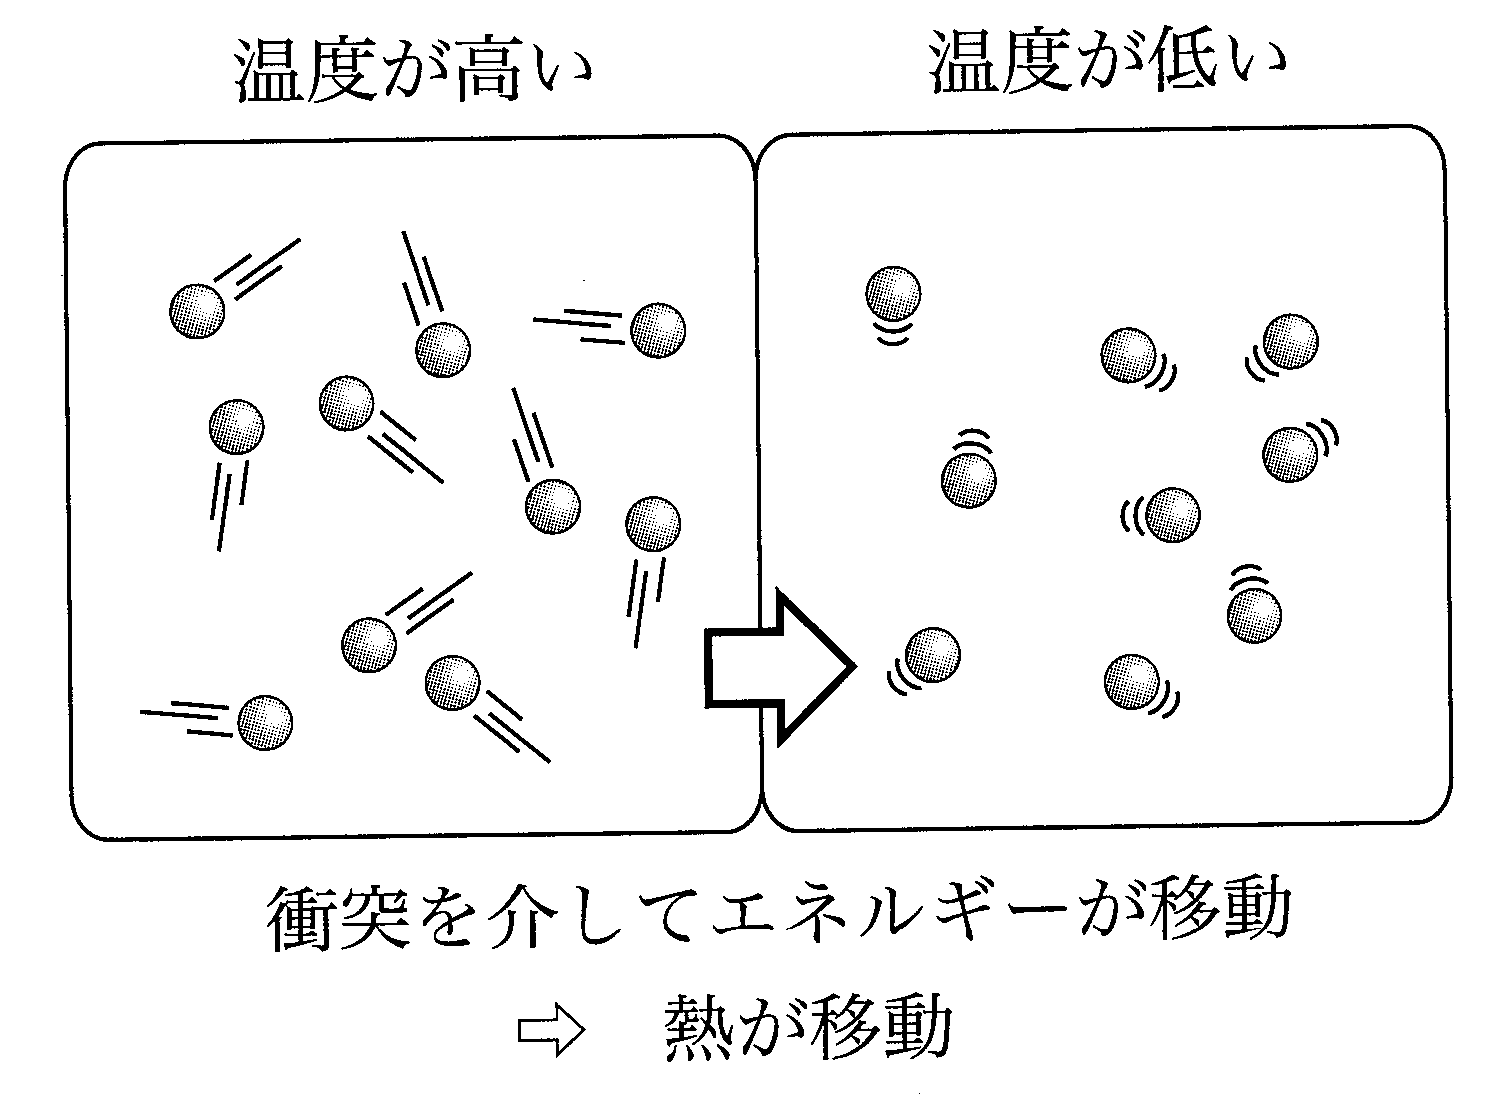
\includegraphics[keepaspectratio,width=70mm]
  {text_p66_fig1.png}
\end{wrapfigure}
熱い物体Aと冷たい物体Bを接触させたときには，Aの温度は下がり，Bの温度は上がるが，これは接触部分での原子・分子の衝突を通してAの原子・分子の運動がBの原子・分子の運動へと移っていくからである．
この現象を，{\bf AからBへ熱が移った}と表現する．

このように熱は本質的には構成原子・分子の微細な運動エネルギーによるものであるから，移動した熱の量はエネルギーの単位[J]を用いて表すことができる．
しかし，通常の熱の移動現象を扱う際には日常生活に密接した単位である{\bf カロリー[cal]}を用いられることも多い．
{\bf 1[cal]は水1[g]の温度を1[K]だけ高めるのに必要な熱量}として定義される．
カロリーとジュールの間には，1[cal]=4.186[J]の関係がある．
この換算率を{\bf 熱の仕事当量}という．
\[ J \fallingdotseq 4.2[{\rm J/cal}] \]

一般の物質の熱しやすさ・冷めやすさは比熱によって表す．
物質1[g]あたりの温度を1[K]上げるのに必要な熱量を{\bf 比熱}\mbox{\boldmath $c$}{\bf [cal/g・K]}という．
比熱を用いると，その物質を温度上昇させるのに必要な熱量が求められる．
その物質の比熱を$c$[cal/g・K]，質量を$m$[g]，上昇させる温度を$\Delta T$[K]とすると，必要な熱量$Q$[cal]は
\[ \mbox{\boldmath $Q=mc\Delta T$} \hspace{2mm} [{\rm cal}] \]
と求められる．

また，ある物体の温度を1[K]上げるのに必要な熱量を{\bf 熱容量}\mbox{\boldmath $C$}{\bf [cal/K]}という．
$C=mc$なる関係式が成立するので，この物体の温度を$\Delta T$[K]だけ上昇させるには，
\[ \mbox{\boldmath $Q=C\Delta T$} \hspace{2mm} [{\rm cal}]\]
だけの熱量が必要である．

温度の異なる二つの物体を接触させると，高温の物体から低温の物体へと熱が移動する．
やがて両者の温度が等しくなると熱の移動は止まる．
この状態を{\bf 熱平衡状態}という．

外部との熱のやり取りがなければ，{\bf 高温の物体が失った熱量と，低温の物体が得た熱量は等しい．}
これを{\bf 熱量の保存}という．
熱平衡状態の温度を文字でおいて，
\[ \mbox{\boldmath （高温の物体が失った熱量）＝（低温の物体が得た熱量）} \]
の形の式を立てれば，その温度が求められる．

このとき，{\bf 液体を入れてある容器も液体と一緒に温度が変わる}ことを忘れてはならない．
容器の熱容量が$C$[cal/K]と与えられていれば，容器が得た熱量として$C\Delta T$[cal]を右辺に加える必要がある．

\begin{matome}{熱の仕事当量・比熱・熱容量}
 \hspace{3mm} $J \fallingdotseq 4.2$\hspace{2mm}[J/cal]\\
\hspace{3mm} $Q=mc\Delta T$\hspace{2mm}[cal]\hspace{10mm} 比熱$c$\hspace{2mm}[cal/g・K]\\
\hspace{3mm} $Q=C\Delta T$\hspace{2mm}[cal]\hspace{13mm} 熱容量$C$\hspace{2mm}[cal/K]\\
\hspace{3mm} 熱量の保存\hspace{9mm} （高温の物体が失った熱量）＝（低温の物体が得た熱量）
\end{matome}

\begin{reidaiunit}
\begin{reidai}{熱の仕事当量}
\hspace{1zw}質量$500\U{g}$の金属塊を$80\Cel$に熱し，$20\Cel$の水$450\U{g}$の中に入れたところ，全体の温度は$30\Cel$となった．容器の熱容量が$50\U{cal/K}$であるとき，この金属の比熱を求めよ．
\end{reidai}

\begin{sisinE}
熱量の保存を使う．金属塊が失った熱量が，水と容器の温度上昇に使われている．{\bf 容器も水と一緒に温度が上がっている}ことを忘れないこと．なお水の比熱は$1\U{cal/g\cdot K}$である．
\end{sisinE}

\Key{$Q=mc\Delta T$\,[cal]\quad $Q=C\Delta T$\,[cal]}

\begin{kaitou}
\hspace{1zw}金属の比熱を$c\U{cal/g\cdot K}$とする．金属塊は$80\Cel$から$30\Cel$まで$50\U{K}$下がり，水と容器はともに$20\Cel$から$30\Cel$まで$10\U{K}$上がる．よって，金属塊が失った熱量$Q\U{cal}$，水が得た熱量$Q'\U{cal}$，容器が得た熱量$Q''\U{cal}$はそれぞれ，
\[Q=500\cdot c\cdot(80-30)=25000c\]
\[Q'=450\cdot 1\cdot(30-20)=4500\]
\[Q''=50\cdot(30-20)=500\]
\hspace{1zw}熱量の保存より，金属塊が失った熱量が水と容器の温度上昇に使われたので，
\[Q=Q'+Q''\]
すなわち，
\[25000c=4500+500=5000\]
よって，
\Ana{c=0.20\U{cal/g\cdot K}\Ans}
\end{kaitou}
\end{reidaiunit}
 
\subsection{熱力学第一法則}

\begin{wrapfigure}[8]{r}[5mm]{90mm}
  \centering
  \vspace{-5mm}
  
\includegraphics[keepaspectratio,width=90mm]
  {text_p67_fig1.png}
\end{wrapfigure}
熱とはエネルギーの一形態であり，物体内部に蓄えられることのできるエネルギーだとみなすことができるが，このように，物体内部に蓄えられるエネルギーのことを{\bf 内部エネルギー}と呼ぶ．
物体に対して熱や仕事といったエネルギーを与えればこの内部エネルギーを増加させることができ，逆に物体が外界に対して熱を放出したり仕事をしたりすればこの内部エネルギーは減少する．
しかし，いかなる場合であってもそのエネルギーの収支関係は必ずつり合う．
これを{\bf 熱力学第一法則}という．

例えば，ある物体に対して外から$Q_{in}$[J]の熱量と，$W_{in}$[J]の仕事を加えたとする．
この場合，これら2つが内部エネルギーの増分$\Delta U$[J]となったのであるから，熱力学第一法則は，
\[ \Delta U=Q_{in}+W_{in}\]
と表される．

内部エネルギーについては常に増加を正とした$\Delta U$で扱うが，{\bf 熱や仕事は，気体に対して加えられたものなのか，気体が外界に対して与えたものなのかが非常に重要である．}気体が外界に対してした仕事$W_{out}$との間には$W_{out}=-W_{in}$の関係が成り立つので，熱力学第一法則は上の式を変形して
\[ Q_{in} =\Delta U +W_{out}\]
の形で扱う方が良い．気体が膨張すると$W_{out}>0$，圧縮すると$W_{out}<0$となる．

\begin{matome}{熱力学第一法則}
 \hspace{3mm} 外部が気体に与えた熱量を$Q_{in}$，気体が外部にした仕事を$W_{out}$，気体の内部エネルギーの増加量を$\Delta U$とすると，
\[ Q_{in}=\Delta U +W_{out}\]
が成り立つ．
\end{matome}

問題によっては，熱や仕事が「気体が放出した熱量」「気体がされた仕事」といった{\bf 逆向き}で与えられていることがある．
その場合は公式にそのまま代入せず，まず$Q_{in}$と$W_{out}$に読み替えてから代入する．
例えば気体が外界に$q$[J]の熱量を放出したのなら$Q_{in}=-q$[J]，外界が気体に$W$[J]の仕事をしたのなら$W_{out}=-W$[J]である．
{\bf 向きを$Q_{in}$，$W_{out}$に揃えてから式に入れる}という手順を守れば符号を間違えない．
\begin{reidaiunit}
\begin{reidai}{熱力学第一法則}
\begin{komon}
\ko{1} 物体が外界に放出した熱量$q\U{J}$，物体が外界からされた仕事$W\U{J}$，物体の内部エネルギー増加$\Delta U\U{J}$の間に成り立つ熱力学第一法則の式を示せ．
\ko{2} 物体が外界に放出した熱量$q\U{J}$，物体が外界に対してした仕事$w\U{J}$，物体の内部エネルギー増加$\Delta U\U{J}$の間に成り立つ熱力学第一法則の式を示せ．
\end{komon}
\end{reidai}

\begin{sisinE}
与えられている熱量・仕事の向きが，公式の$Q_{in}$（外部が気体に与えた熱量）・$W_{out}$（気体が外部にした仕事）と逆になっている．公式にそのまま代入せず，まず$Q_{in}$と$W_{out}$に読み替えてから代入する，という手順を守ればよい．
\end{sisinE}

\Key{熱量・仕事の出入りを把握 $\Rightarrow$ 熱力学第一法則の利用}

\begin{kaitou}
\begin{komon}
\ko{1} 物体が外界に$q\U{J}$の熱量を放出したのだから，外部が物体に与えた熱量は$Q_{in}=-q\U{J}$である．また，物体が外界からされた仕事が$W\U{J}$なのだから，物体が外界にした仕事は$W_{out}=-W\U{J}$である．これらを$Q_{in}=\Delta U+W_{out}$に代入して，
       \[-q=\Delta U+(-W)\]
       よって，
       \Ana{\Delta U=-q+W\U{J}\Ans}
\ko{2} (1)と同様に$Q_{in}=-q\U{J}$である．今度は物体が外界にした仕事が$w\U{J}$なのだから，$W_{out}=w\U{J}$である．よって，
       \[-q=\Delta U+w\]
       すなわち，
       \Ana{\Delta U=-q-w\U{J}\Ans}
\end{komon}
\end{kaitou}
\end{reidaiunit}






\subsection{熱力学第二法則}

世の中の物理現象には，ある変化A$\rightarrow$Bに対して，それを完全に時間に対して逆行させることのできる変化と，それができない変化の2つがある．
前者を{\bf 可逆変化}といい，後者を{\bf 不可逆変化}という．

\begin{wrapfigure}[4]{r}[5mm]{70mm}
  \centering
  \vspace{-5mm}
  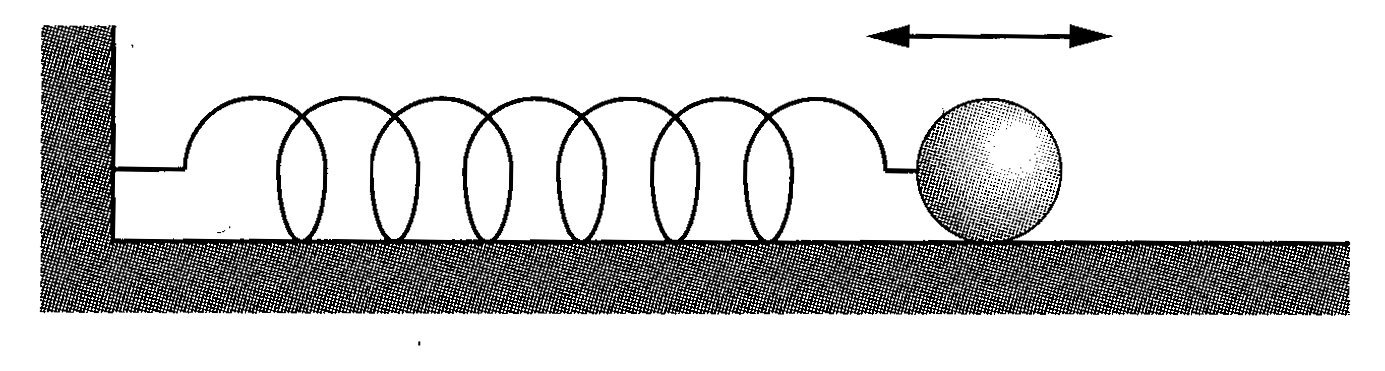
\includegraphics[keepaspectratio,width=70mm]
  {text_p68_fig1.png}
\end{wrapfigure}
例えば図のような床面上での単振動を考えてみる．
もし床面に完全に摩擦がなく，空気抵抗もなければこの振動は永久に続き，その力学的エネルギーは一定に保たれる．
これは可逆変化である．

しかし実際には床面には必ずわずかながらの摩擦があり，空気抵抗もある．
そのため，単振動の振幅は減衰してついには止まる．
この最中に失われた力学的エネルギーは摩擦熱などとなっておもりを温めたり空気中に拡散していく．
しかしこの逆の現象，すなわち静止しているおもりが周囲から熱を自発的に吸収してひとりでに振動することは決してない．
このような変化を不可逆変化という．

また同様に，高温の物体Aと低温の物体Bとを接触させておくと，AからBへと熱が流れ，両者は等しい温度となるが，この逆の現象，すなわち等しい温度となっている2つの物体A，Bの片方からもう片方へ熱が移動し，低温の物体から高温の物体へ熱が移動することは決してない．
これも不可逆変化である．

このような，熱の発生現象や熱伝導現象は不可逆変化であるが，これらの不可逆変化の逆方向の変化はエネルギーの出入りが逆になるだけであるからエネルギー保存則に矛盾しているわけではない．
そうした不可逆反応について，どちらの方向へ進むのは可能でどちらは不可能なのかを支配しているのが{\bf 熱力学第二法則}である．

\begin{matome}{熱力学第二法則}
 \hspace{3mm} ある温度の熱源から熱を奪って自分の力学的エネルギーに変え，かつ自分と周囲のものが元の状態に戻るような変化はできない．
\end{matome}

熱力学第二法則には他にもいろいろな表現法がある．
その代表的な表現を2つ挙げる．

\Kou{1}{トムソンの原理}

熱が自発的に力学的な仕事・エネルギーに変化することはない．\\

\Kou{2}{クラウジウスの原理}

熱が低温の物体から高温の物体へ自発的に移ることはない．\\

この2つは表現こそ違うが同じ内容を述べており，対偶をとることで互いに導き合うことができる．

\newpage

%%%%%%%%%%%%%%%%%%%%  練習問題（旧 prob_p35.png / prob_p36.png）  %%%%%%%%%%%%%%%%%%%%
% 第2章（熱力学）から問題番号を［1］に振り直す（原本もここで番号がリセットされている）
\setcounter{qno}{0}

\Rank{A問題}

\Mon{基本事項の確認}

\hspace{1zw}以下の設問に答えよ．ただし，気体定数は$8.31\U{J/mol\cdot K}$である．
\begin{komon}
\ko{1} シリンダー内に断面積$1.0\times 10^{-2}\U{m^2}$のピストンで閉じ込められた気体が，$5.0\U{N}$の力でピストンを押している．この気体の圧力は何$\U{Pa}$か．有効数字2桁で求めよ．
\ko{2} 酸素気体$\mathrm{O_2}$ $96\U{g}$中に含まれている酸素分子の数は何個か．ただし，アボガドロ数を$N_{\mathrm{A}}=6.02\times 10^{23}$\,[個/mol]とする．有効数字2桁で求めよ．
\ko{3} 温度$20\Cel$の水$300\U{g}$を$100\Cel$まで加熱するのに必要な熱量は何$\U{cal}$か．またこれは何$\U{J}$か．ただし，熱の仕事当量を$J=4.2\U{J/cal}$とする．有効数字2桁で求めよ．
\ko{4} 質量$200\U{g}$の金属塊の温度を$20\Cel$から$60\Cel$まで加熱するのに要する熱量が$56000\U{cal}$であった．この金属の比熱は何$\U{cal/g\cdot K}$か．また，この金属塊の熱容量は何$\U{cal/K}$か．有効数字2桁で求めよ．
\end{komon}

\Rank{B問題}

\Mon{状態方程式}

\hspace{1zw}容器中に理想気体が入っており，圧力$p_0\U{Pa}$，体積$V_0\U{m^3}$におけるその気体の温度を$T_0\U{K}$とする．
\begin{komon}
\ko{1} 温度を$T_0\U{K}$に保ったまま，体積を$kV_0\U{m^3}$になるまで膨張したときの気体の圧力を求めよ．
\ko{2} 圧力を$p_0\U{Pa}$に保ったまま，温度が$kT_0\U{K}$になるまで加熱したときの気体の体積を求めよ．
\ko{3} 体積を$V_0\U{m^3}$に保ったまま，圧力が$kp_0\U{Pa}$になるまで熱したときの気体の温度を求めよ．
\ko{4} この気体を熱し続けて温度が$t_1\Cel$になったとき，圧力が$p_1\U{Pa}$であったとする．$0\Cel=273.15\U{K}$として，気体の体積を求めよ．
\end{komon}

\Mon[\Sitei]{状態方程式}

\begin{zuright}{47mm}
\hspace{1zw}右図のように断熱材でできた自由に動くことのできるピストン$\mathrm{C}$で，長さ$l_{\mathrm{A}}\U{m}$の$\mathrm{A}$と長さ$l_{\mathrm{B}}\U{m}$の$\mathrm{B}$の二つの部分に分けられた容器があり，$\mathrm{A}$，$\mathrm{B}$にはともに温度$T_0\U{K}$，圧力$p_0\U{Pa}$の理想気体が入っている．$\mathrm{A}$内の気体はそのままにし，$\mathrm{B}$内の気体だけを温めて温度を$T_1\U{K}$に上げて保ったところ，$\mathrm{C}$は$l\U{m}$だけ移動した．
\begin{komon}
\ko{1} $\mathrm{C}$はどちら向きへ移動するか．
\ko{2} 移動後の$\mathrm{A}$内の気体の温度および，$\mathrm{A}$，$\mathrm{B}$内の気体の圧力を求めよ．
\end{komon}
\zusep
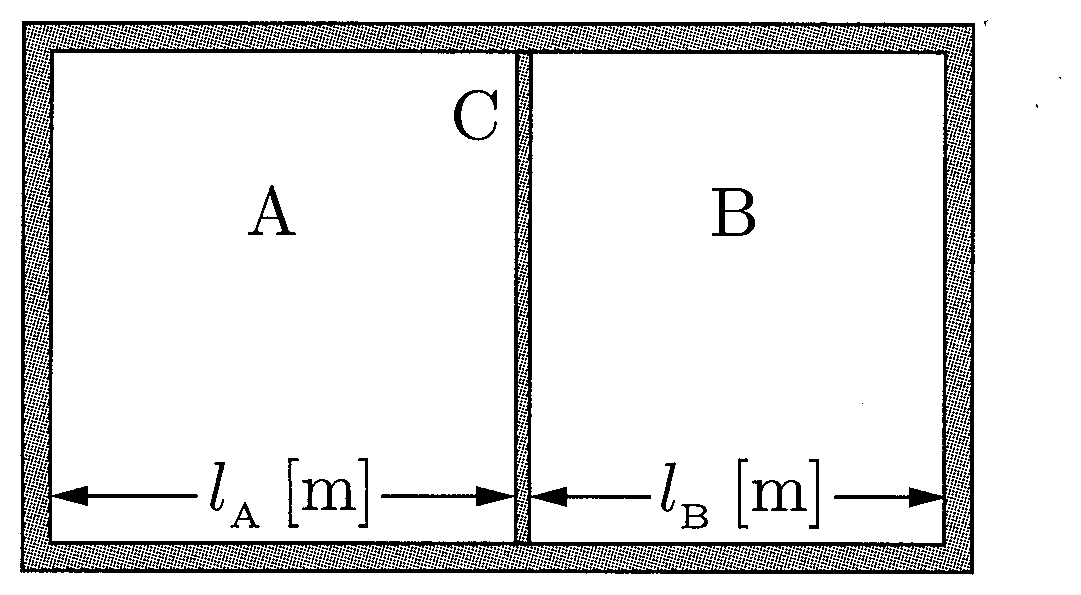
\includegraphics[keepaspectratio,width=47mm]{fig/ch14_p35_cyl.png}
\end{zuright}

\Mon[\Sitei]{熱量の保存}

\hspace{1zw}比熱$c_{\mathrm{A}}\U{cal/g\cdot K}$，質量$m_{\mathrm{A}}\U{g}$，温度$t_{\mathrm{A}}\Cel$の金属$\mathrm{A}$と，比熱$c_{\mathrm{B}}\U{cal/g\cdot K}$，質量$m_{\mathrm{B}}\U{g}$，温度$t_{\mathrm{B}}\Cel$の金属$\mathrm{B}$を接触させ十分時間が経ったところ，$\mathrm{A}$，$\mathrm{B}$間で熱のやり取りが行われ，熱平衡状態に達した．$t_{\mathrm{A}}>t_{\mathrm{B}}$として以下の問に答えよ．
\begin{komon}
\ko{1} 熱平衡状態における$\mathrm{A}$，$\mathrm{B}$の温度を求めよ．
\ko{2} このとき$\mathrm{A}$の失った熱量および$\mathrm{B}$が得た熱量を求めよ．
\end{komon}

\Mon{熱量の保存}

\hspace{1zw}質量$M\U{g}$の銅製の容器（温度$t_0\Cel$）に温度$t_0\Cel$の水が$w\U{g}$入っている．この中へ温度$t\Cel$（$t>t_0$），質量$m\U{g}$の銅球を入れてかきまぜたところ，全体の温度は一様に$t'\Cel$になった．これらを元に，銅の比熱を求めよ．
% 誤植訂正（2026-08-29）：元の問題集は「この中への温度 t[C]（t>t_0），質量 m[g] の銅球を
%   入れて」となっていたが，「この中へ温度 t[C]…の銅球を入れて」が正しい（「への」の「の」が余分）．

\Mon{摩擦熱}

\hspace{1zw}時速$72\U{km/h}$で走っている質量$1\U{t}$の自動車がブレーキをかけたところ，自動車は摩擦のため静止した．摩擦によって生じた熱量は何$\U{cal}$か．ただし熱の仕事当量を$J=4.2\U{J/cal}$とする．

\Mon{熱力学第一法則}

\hspace{1zw}ある気体が状態変化する際，気体に外界から加えられた熱量，気体の内部エネルギーの増加量，そして気体が外界に対してした仕事がそれぞれ$Q\U{J}$，$\Delta U\U{J}$，$W\U{J}$であった．これについて以下の問に答えよ．
\begin{komon}
\ko{1} $Q$, $\Delta U$, $W$の間に成り立つ熱力学第一法則を記せ．
\end{komon}
\hspace{1zw}またこの状態変化の際の仕事・熱のやり取りを，気体が熱を外界に放出し，気体が外界から仕事をされたとして捉え，それぞれの量を$Q'\U{J}$，$W'\U{J}$とおく．
\begin{komon}
\ko{2} $Q'$, $\Delta U$, $W'$の間に成り立つ関係式を求めよ．
\end{komon}

\Rank{C問題}

\Mon{状態方程式}

\begin{zuright}{41mm}
\hspace{1zw}図のように容積の等しい二つの容器$\mathrm{A}$，$\mathrm{B}$が細管でつながれ，コック$\mathrm{C}$を通して温度$T_1\U{K}$，圧力$P_1\U{Pa}$の大気に通じている．はじめコック$\mathrm{C}$は開かれており，容器および内部の気体の温度はすべて大気と同じ温度であった．細管の容積と容器の熱膨張を無視し，空気は理想気体とみなしてよいものとして以下の問に答えよ．
\zusep
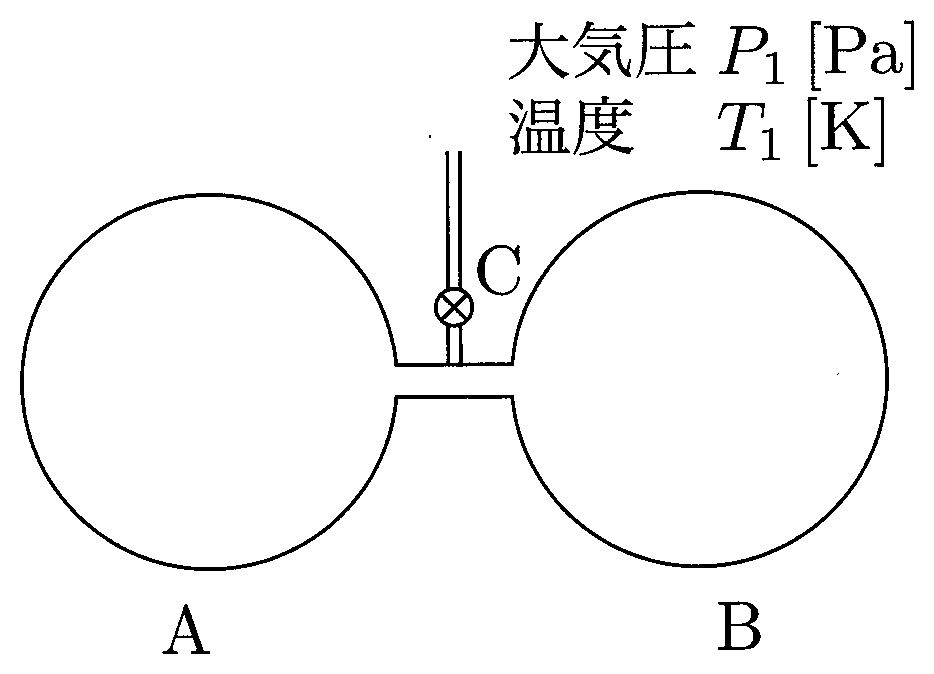
\includegraphics[keepaspectratio,width=41mm]{fig/ch14_p36_flask.png}
\end{zuright}
\vspace{-\medskipamount}
\begin{komon}
\ko{1} コック$\mathrm{C}$を開いたまま，$\mathrm{B}$は大気と同じ温度に保ちつつ$\mathrm{A}$の温度を$T_0\U{K}$になるまでゆっくりと冷やした．$\mathrm{A}$を冷やしている間に$\mathrm{A}$，$\mathrm{B}$に流入した気体のモル数は，はじめ$\mathrm{B}$の中にあった空気のモル数の何倍か．
\ko{2} 次にコック$\mathrm{C}$を閉じ，$\mathrm{A}$をゆっくりと温めて，$\mathrm{A}$および$\mathrm{B}$の温度を再び大気の温度に等しくした．このときの$\mathrm{A}$，$\mathrm{B}$内の空気の圧力$P_2\U{Pa}$を求めよ．
\end{komon}

\Mon{熱力学第二法則}

\hspace{1zw}次の文の空欄に当てはまる語を下記の語群の中から選び，その記号で答えよ．ただし，重複して用いてもよいものとする．

\hspace{1zw}熱力学第二法則は，\framebox[3zw]{ア}変化に関係した法則で，さまざまな表現の仕方がある．
\begin{quote}
\noindent $\mathrm{I}$\hspace{2zw}クラウジウスの原理\par
\hspace{2zw}他に影響を与えないで，熱を\framebox[3zw]{イ}温の物体から\framebox[3zw]{ウ}温の物体に移すことはできない．\par
\noindent $\mathrm{I\!I}$\hspace{2zw}トムソンの原理\par
\hspace{2zw}与えられた\framebox[3zw]{エ}をすべて\framebox[3zw]{オ}に変えてしまうような熱機関をつくることはできない．
\end{quote}
\hspace{1zw}$\mathrm{I}$と$\mathrm{I\!I}$は，同じ内容を違う表現で述べてあるにすぎない．同値であることは，数学でよく用いられる対偶法によって証明することができる．これを考えてみよう．

\hspace{1zw}もし，$\mathrm{I\!I}$が成り立たないとすると，\framebox[3zw]{カ}温の熱源からもらった熱をすべて\framebox[3zw]{キ}に変えることができるから，これを\framebox[3zw]{ク}温の熱源に与えれば\framebox[3zw]{ケ}を与えたのと同じことになるので，他に影響を与えないで熱が\framebox[3zw]{コ}温の物体から\framebox[3zw]{サ}温の物体に移ったことになり，$\mathrm{I}$が否定されてしまう．同様に$\mathrm{I}$が成り立たないとすると，$\mathrm{I\!I}$が否定されるので，$\mathrm{I}$と$\mathrm{I\!I}$とは同値の関係にあると言える．

\begin{bsHosoku}{選択肢}
\noindent\hspace*{1zw}A\hspace{1zw}熱\hfill B\hspace{1zw}仕事\hfill C\hspace{1zw}高\hfill D\hspace{1zw}低\hfill E\hspace{1zw}可逆\hfill F\hspace{1zw}不可逆\hspace*{1zw}
\end{bsHosoku}

\newpage

%%%%%%%%%%%%%%%%%%%%  解答（旧 prob_p117〜p120_1.png）  %%%%%%%%%%%%%%%%%%%%
% 回タイトルは段組の“外”で出す（2.5ptの罫をページ全幅に引くため）
\KaiTitle{第14回　気体の状態方程式・熱力学第一法則}

\setlength{\columnseprule}{0.4pt}
\begin{multicols}{2}
\raggedcolumns

\Rank{A問題}
\MonN{1}{基本事項の確認}
\begin{saikei}
圧力，酸素分子の数，水の加熱に必要な熱量，金属の比熱と熱容量を求める．
\end{saikei}
\begin{sisin}
状態方程式$PV=nRT$や圧力と力の関係式$F=PS$などの関係式を利用せよ．
\end{sisin}
\begin{kaitou}
\begin{komon}
\ko{1} $P=\dfrac{F}{S}=\dfrac{5.0}{1.0\times 10^{-2}}=5.0\times 10^2\U{Pa}$\Ans
\ko{2} $\mathrm{O_2}$の分子量は$M=32\U{g/mol}$なので，$96\U{g}$は$n=\dfrac{w}{M}=\dfrac{96}{32}=3.0\U{mol}$に相当．よって，分子数は
       \[\begin{aligned}
         N&=n\cdot N_{\mathrm{A}}=3.0\times 6.02\times 10^{23}\\
          &\fallingdotseq 1.8\times 10^{24}\,\text{[個]}\Ans
       \end{aligned}\]
\ko{3} 水の比熱は$1\U{cal/g\cdot K}$であるから，
       \[\begin{aligned}
         Q&=mc\Delta t=300\cdot 1\cdot(100-20)\\
          &=2.4\times 10^4\U{cal}
       \end{aligned}\]
       また，$1\U{cal}=4.2\U{J}$なので，
       \[Q=2.4\times 10^4\times 4.2\U{J}\fallingdotseq 1.0\times 10^5\U{J}\Ans\]
\ko{4} $Q=mc\Delta t$より，$56000=200\times c\times(60-20)$が成り立つから，
       \[c=\frac{56000}{200\cdot(60-20)}=7.0\U{cal/g\cdot K}\]
       また，熱容量は，
       \[\begin{aligned}
         C&=m\cdot c=7.0\times 200\\
          &=1.4\times 10^3\U{cal/K}\Ans
       \end{aligned}\]
\end{komon}

\end{kaitou}
\Rank{B問題}
\MonN{2}{状態方程式}
\begin{saikei}
圧力$p_0$，体積$V_0$，温度$T_0$の理想気体について，等温・等圧・等積の各変化後の量を求める．
\end{saikei}
\begin{sisin}
状態方程式$PV=nRT$を元にして考える．ある量を固定して他の量を変化させる場合には，左辺もしくは右辺に変化しない量をまとめてしまうのがコツである．例えば(2)の変化では，気体の圧力が一定なので，状態方程式で一定の量の$n$, $R$, $p$を右辺にまとめると，$\dfrac{V}{T}=\dfrac{nR}{p}=$（一定）となり，$\dfrac{V}{T}$が変化していないことが分かる．
\end{sisin}
\begin{kaitou}
\hspace{1zw}気体が$n\U{mol}$あるとする．また，気体定数を$R\U{J/mol\cdot K}$とする．
\begin{komon}
\ko{1} この状態変化では気体の温度が一定であるから，理想気体の状態方程式の$n$, $R$, $T$が一定に保たれる．よって状態方程式より，$pV=nRT=$（一定）となる．変化後の気体の圧力を$p'\U{Pa}$とすれば，
       \[p'\cdot kV_0=p_0\cdot V_0\]
       ゆえに，
       \[p'=\frac{1}{k}p_0\U{Pa}\Ans\]
\ko{2} この状態変化では気体の圧力が一定であるから，理想気体の状態方程式の$n$, $R$, $p$が一定に保たれる．よって状態方程式より，$\dfrac{V}{T}=\dfrac{nR}{p}=$（一定）となる．変化後の気体の体積を$V'\U{m^3}$とすれば，
       \[\frac{V'}{kT_0}=\frac{V_0}{T_0}\]
       ゆえに，
       \[V'=kV_0\U{m^3}\Ans\]
\ko{3} この状態変化では気体の体積が一定であるから，理想気体の状態方程式の$n$, $R$, $V$が一定に保たれる．よって状態方程式より，$\dfrac{p}{T}=\dfrac{nR}{V}=$（一定）となる．変化後の気体の温度を$T'\U{K}$とすれば，
       \[\frac{kp_0}{T'}=\frac{p_0}{T_0}\]
       ゆえに，
       \[T'=kT_0\U{K}\Ans\]
\ko{4} この状態変化においては圧力，体積，温度が変化するので状態方程式をそのまま利用する．始めの状態の状態方程式は，
       \[p_0V_0=nRT_0\]
       変化後の状態方程式は，絶対温度が$t_1+273.15\U{K}$であることに注意して，変化後の体積を$V_1\U{m^3}$とすると，
       \[p_1V_1=nR(t_1+273.15)\]
       以上2式から$n$, $R$を消して$V_1$を求めると，
       \[V_1=\frac{p_0(t_1+273.15)}{p_1T_0}V_0\U{m^3}\Ans\]
\end{komon}
\end{kaitou}
\begin{chuu}
\hspace{1zw}上の解答では状態方程式を変形することで答えを導いたが，(4)と同様に，変化前・変化後の二つの状態方程式から答えを導いてもよい．例えば(2)であれば，変化前の状態方程式$p_0V_0=nRT_0$と，変化後の状態方程式$p_0V'=nR(kT_0)$の二つの組み合わせから，$V'=kV_0\U{m^3}$を導くことが可能である．
\end{chuu}

\MonN{3}{状態方程式}
\begin{saikei}
断熱ピストン$\mathrm{C}$で二分された容器．$\mathrm{B}$だけを$T_1$に温めたときの$\mathrm{C}$の移動の向き，$\mathrm{A}$の温度，$\mathrm{A}$，$\mathrm{B}$の圧力を求める．
\end{saikei}
\begin{sisin}
ピストン$\mathrm{C}$は$\mathrm{A}$，$\mathrm{B}$の気体から圧力を受けるが，例えば$\mathrm{A}$からの圧力の方が大きければピストンは右へ移動する．よって，ピストンが静止しているときは$\mathrm{A}$，$\mathrm{B}$の圧力は等しい．また，$\mathrm{C}$は断熱材であるから，$\mathrm{A}$，$\mathrm{B}$の温度は等しくなくてもよい．

本問のような問題では，変化前・変化後の気体の状態方程式を立てて考えるのが基本である．問題文では状態方程式を立てるのに必要な変数がすべて与えられていないので，適宜仮定した上で状態方程式を立てよう．
\end{sisin}
\begin{kaitou}
\hspace{1zw}ピストン$\mathrm{C}$の断面積を$S\U{m^2}$，$\mathrm{A}$，$\mathrm{B}$内の気体の物質量を$n_{\mathrm{A}}\U{mol}$，$n_{\mathrm{B}}\U{mol}$とし，気体定数を$R\U{J/mol\cdot K}$とすると，最初の状態についての状態方程式より，
\[\mathrm{A}:p_0(Sl_{\mathrm{A}})=n_{\mathrm{A}}RT_0\Eq{1}\]
\[\mathrm{B}:p_0(Sl_{\mathrm{B}})=n_{\mathrm{B}}RT_0\Eq{2}\]
である．
\begin{komon}
\ko{1} $\mathrm{B}$内の気体の温度を上げると，$\mathrm{B}$内の気体の圧力の方が$\mathrm{A}$内の気体の圧力より大きくなってしまうので，ピストン$\mathrm{C}$は$\mathrm{B}$から$\mathrm{A}$の向きへ移動する．\Ans
\ko{2} ピストン$\mathrm{C}$は自由に動くことができるので，ピストン$\mathrm{C}$が移動して静止した時の$\mathrm{A}$，$\mathrm{B}$内の気体の圧力は等しい．これを$p\U{Pa}$とする．また，このときの$\mathrm{A}$内の気体の温度を$T\U{K}$とすると，変化後のシリンダーの長さがそれぞれ$l_{\mathrm{A}}-l$, $l_{\mathrm{B}}+l$になっていることに注意して，
       \[\mathrm{A}:p\cdot S(l_{\mathrm{A}}-l)=n_{\mathrm{A}}RT\Eq{3}\]
       \[\mathrm{B}:p\cdot S(l_{\mathrm{B}}+l)=n_{\mathrm{B}}RT_1\Eq{4}\]
       が成立する．これと先に立てた状態方程式を組み合わせる．\MARU{2}，\MARU{4}より，
       \[p=\frac{l_{\mathrm{B}}T_1}{(l_{\mathrm{B}}+l)T_0}p_0\U{Pa}\Ans\]
       また，\MARU{1}，\MARU{3}および$p$より，
       \[T=\frac{(l_{\mathrm{A}}-l)l_{\mathrm{B}}}{(l_{\mathrm{B}}+l)l_{\mathrm{A}}}T_1\U{K}\Ans\]
\end{komon}
\end{kaitou}
\begin{chuu}
\hspace{1zw}$\mathrm{A}$内の気体の温度が変化することに注意．
\[\mbox{「熱の出入りがない」}\]
\[=\mbox{「温度が変化しない」}\]
と考えるのは間違いである．
\end{chuu}

\MonN{4}{熱量の保存}
\begin{saikei}
温度の違う金属$\mathrm{A}$，$\mathrm{B}$を接触させたときの熱平衡温度と，やり取りした熱量を求める．
\end{saikei}
\begin{sisin}
一般的に，熱は温度の高いものから低いものへと移っていき，最終的には両者の温度が等しくなって熱の移動が止まる．この状態を「熱平衡状態」と呼ぶ．

熱量の保存より，$\mathrm{A}$が失った熱量分を$\mathrm{B}$が受け取っている．よって，熱平衡状態の温度を適当な文字でおき，$\mathrm{A}$が失った熱量と$\mathrm{B}$が得た熱量をその文字で表して考える．
\end{sisin}
\begin{kaitou}
\begin{komon}
\ko{1} 熱平衡状態における$\mathrm{A}$，$\mathrm{B}$の温度を$t\Cel$とする．この状態に至るまでに，$\mathrm{A}$の温度は$t_{\mathrm{A}}-t$だけ下がり，$\mathrm{B}$の温度は$t-t_{\mathrm{B}}$だけ上がる．よって$\mathrm{A}$が失った熱量$Q_{\mathrm{A}}\U{cal}$および$\mathrm{B}$が得た熱量$Q_{\mathrm{B}}\U{cal}$は，
       \[Q_{\mathrm{A}}=m_{\mathrm{A}}c_{\mathrm{A}}(t_{\mathrm{A}}-t),\]
       \[Q_{\mathrm{B}}=m_{\mathrm{B}}c_{\mathrm{B}}(t-t_{\mathrm{B}})\]
       \hspace{1zw}熱量の保存より，$\mathrm{A}$が失った熱量と$\mathrm{B}$が得た熱量は等しいので，
       \[m_{\mathrm{A}}c_{\mathrm{A}}(t_{\mathrm{A}}-t)=m_{\mathrm{B}}c_{\mathrm{B}}(t-t_{\mathrm{B}})\]
       である．これを解いて，
       \[t=\frac{m_{\mathrm{A}}c_{\mathrm{A}}t_{\mathrm{A}}+m_{\mathrm{B}}c_{\mathrm{B}}t_{\mathrm{B}}}{m_{\mathrm{A}}c_{\mathrm{A}}+m_{\mathrm{B}}c_{\mathrm{B}}}\Cel\Ans\]
\ko{2} (1)の$t$を$Q_{\mathrm{A}}$, $Q_{\mathrm{B}}$の式に代入して，
       \[Q_{\mathrm{A}}=Q_{\mathrm{B}}=\frac{m_{\mathrm{A}}c_{\mathrm{A}}m_{\mathrm{B}}c_{\mathrm{B}}(t_{\mathrm{A}}-t_{\mathrm{B}})}{m_{\mathrm{A}}c_{\mathrm{A}}+m_{\mathrm{B}}c_{\mathrm{B}}}\U{cal}\]
       \hspace*{\fill}\Ans
\end{komon}

\end{kaitou}
\MonN{5}{熱量の保存}
\begin{saikei}
銅製の容器・水・銅球が熱平衡に達したときの温度から，銅の比熱を求める．
\end{saikei}
\begin{sisin}
最終的に全体の温度が$t'\Cel$になったのであるから，水，銅球だけでなく容器の温度も変化している．熱の移動を考えれば，銅球が失った熱量は水，容器の温度上昇に利用されている．これを表す式を立てればよい．
\end{sisin}
\begin{kaitou}
\hspace{1zw}銅の比熱を$c\U{cal/g\cdot K}$とする．この変化にて銅球は$t-t'$だけ温度が下がり，水と容器はともに$t'-t_0$だけ温度が上がったので，銅球が失った熱量$Q\U{cal}$，水，熱量計が得た熱量$Q'\U{cal}$，$Q''\U{cal}$はそれぞれ，
\[Q=mc(t-t')\]
\[Q'=w\cdot 1\cdot(t'-t_0)\]
\hspace*{2zw}（注：水の比熱は$1\U{cal/g\cdot K}$）
% 誤植訂正（2026-08-29）：元の問題集はこの注が Q''=Mc(t'-t_0) の行に置かれていたが，
%   注が説明しているのは Q' の式に現れる「1」（水の比熱）なので Q' の行に移した．
%   Q'' は銅製の容器の式で，比熱は c であり 1 ではない．
\[Q''=Mc(t'-t_0)\]
\hspace{1zw}熱量の移動を考えると，銅球が失った熱量が，水と容器の温度上昇に利用されたので，
\[Q=Q'+Q''\]
以上をまとめると，
\[c=\frac{w(t'-t_0)}{m(t-t')-M(t'-t_0)}\U{cal/g\cdot K}\]
\hspace*{\fill}\Ans

\end{kaitou}
\MonN{6}{摩擦熱}
\begin{saikei}
$72\U{km/h}$で走る$1\U{t}$の自動車が静止するまでに生じた摩擦熱を$\U{cal}$で求める．
\end{saikei}
\begin{sisin}
自動車がブレーキをかけると摩擦力の作用により車は静止する．これをエネルギー的な観点から見ると，摩擦力によって自動車の持っていた力学的エネルギーが減少し，その減少分は熱として空気中などに散逸している．この熱を\underline{摩擦熱}という．最終的に静止したのだから，持っていた運動エネルギーすべてが摩擦熱に転化したことになる．

また運動エネルギーを求める際には，まず速さ，質量をMKS単位系に直してエネルギーを$\U{J}$単位で求めよう．
\end{sisin}
\begin{kaitou}
\hspace{1zw}ブレーキをかける前に自動車がもっていた運動エネルギーを$E\U{J}$とする．
\[1\U{t}=1000\U{kg}\]
\[72\U{km/h}=\frac{72000\U{m}}{3600\U{s}}=20\U{m/s}\]
であるから，
\[\begin{aligned}
  E&=\frac{1}{2}mv^2=\frac{1}{2}\cdot 1000\cdot 20^2\\
   &=2.0\times 10^5\U{J}
\end{aligned}\]
\hspace{1zw}摩擦によって失われた運動エネルギーはすべて摩擦熱となったので，このとき生じた熱量は$2.0\times 10^5\U{J}$である．これを$\U{cal}$単位に換算して，
\[Q=\frac{2.0\times 10^5}{4.2}\fallingdotseq 4.8\times 10^4\U{cal}\Ans\]

\end{kaitou}
\MonN{7}{熱力学第一法則}
\begin{saikei}
$Q$，$\Delta U$，$W$の間の熱力学第一法則と，熱・仕事の向きを逆にとったときの関係式を書く．
\end{saikei}
\begin{sisin}
熱力学第一法則を考える際には，熱量，仕事の出入りを把握するのが第一である．それを把握したら，簡単な図を描いてエネルギー収支を日本語で考え，それを式として表せばよい．

熱や仕事のやり取りを，気体に対して加えられたとみなして考えた場合と，気体が外界に対して放出したとみなして考えた場合とは，正負が逆になる．
\end{sisin}
\begin{kaitou}
\begin{komon}
\ko{1} 外部が気体に与えた熱量は$Q$，外部が気体にした仕事は$-W$，気体の内部エネルギーの増加量は$\Delta U$であるから，
       \[\Delta U=Q+(-W)\Ans\]
       \begin{center}
       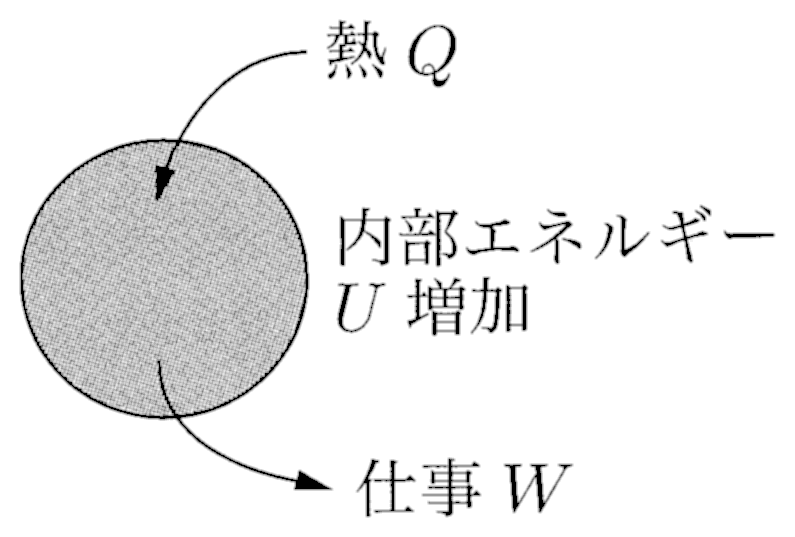
\includegraphics[keepaspectratio,width=38mm]{fig/ch14_p119_dU1.png}
       \end{center}
\ko{2} 外部が気体に与えた熱量は$-Q'$，外部が気体にした仕事は$W'$，気体の内部エネルギーの増加量は$\Delta U$であるから，
       \[\Delta U=(-Q')+W'\Ans\]
       \begin{center}
       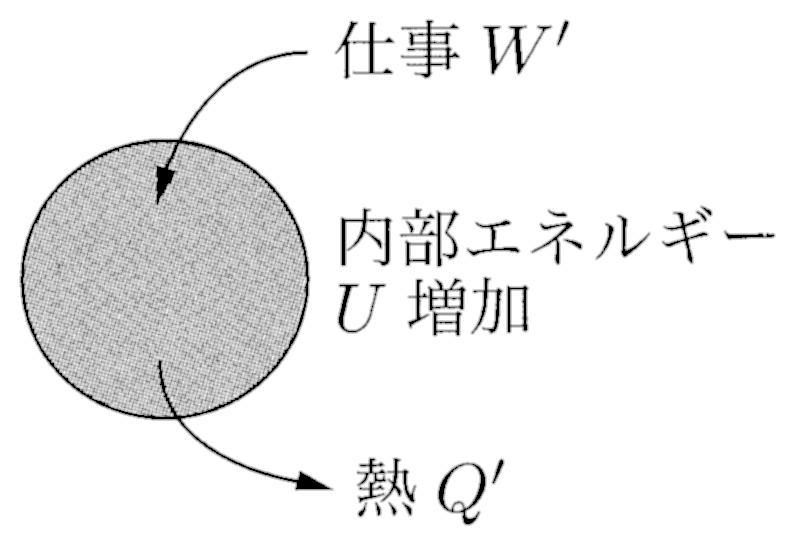
\includegraphics[keepaspectratio,width=38mm]{fig/ch14_p119_dU2.png}
       \end{center}
\end{komon}

\end{kaitou}
\Rank{C問題}
\MonN{8}{状態方程式}
\begin{saikei}
細管でつながれた容器$\mathrm{A}$，$\mathrm{B}$．$\mathrm{A}$を冷やしたときの流入モル数と，コックを閉じて温め直したときの圧力を求める．
\end{saikei}
\begin{sisin}
各状態において，各々の部分の圧力，体積，気体のモル数，温度がどのようになっているのかを考えて，$\mathrm{A}$内および$\mathrm{B}$内の状態方程式を立式し，これを整理せよ．

$\mathrm{A}$と$\mathrm{B}$は細管でつながれているが，$\mathrm{A}$と$\mathrm{B}$とに圧力差がある場合には圧力の高い方から低い方へと気体が移動してしまう．よって，\underline{定常状態においては}\hskip0pt\underline{$\mathrm{A}$と$\mathrm{B}$の}\hskip0pt\underline{気体の圧力は}\hskip0pt\underline{等しくなっている}．しかし，$\mathrm{A}$と$\mathrm{B}$との温度が等しいとは限らないことに注意．$\mathrm{A}$，$\mathrm{B}$の温度は独立に保つことができる．
\end{sisin}
\begin{kaitou}
\hspace{1zw}$\mathrm{A}$，$\mathrm{B}$の体積を$V_0\U{m^3}$，気体定数を$R\U{J/mol\cdot K}$とする．$\mathrm{A}$と$\mathrm{B}$は細管でつながれているので，常に$\mathrm{A}$，$\mathrm{B}$内の気体の圧力は等しくなっている．
\begin{komon}
\ko{1} 今，コック$\mathrm{C}$を開いているので，$\mathrm{A}$，$\mathrm{B}$内の気体の圧力は外界の圧力$P_1$に等しくなっている．この状態における$\mathrm{A}$，$\mathrm{B}$それぞれの中にある気体のモル数を$n_0\U{mol}$とすると，状態方程式より
       \[\mathrm{A},\ \mathrm{B}:P_1V_0=n_0RT_1\]
       が成立する．この状態から，コック$\mathrm{C}$を開いたまま（＝$\mathrm{A}$，$\mathrm{B}$内の気体の圧力を$P_1$に保ったまま）$\mathrm{B}$の温度を$T_1$に，$\mathrm{A}$の温度を$T_0$にした．この変化後の$\mathrm{B}$の状態方程式は
       \[\mathrm{B}:P_1V_0=n_0RT_1\]
       のまま変わらないので，$\mathrm{B}$内の気体のモル数は$n_0$のまま変わらない．変化後の$\mathrm{A}$内の気体のモル数を$n_1\U{mol}$とすると，変化後の$\mathrm{A}$の状態方程式は，
       \[\mathrm{A}:P_1V_0=n_1RT_0\]
       となる．$\mathrm{B}$内の気体のモル数は不変ゆえ$\mathrm{A}$内の気体のモル数の変化のみ考えればよく，$\mathrm{A}$を冷却していく間に流入した気体のモル数（＝$\mathrm{A}$内の気体のモル数の増加量）は，
       \[\Delta n_{\mathrm{A}}=n_1-n_0\]
       であり，これがはじめ$\mathrm{B}$内にあった気体のモル数$n_0$の何倍となるかを求めると，
       \[\frac{\Delta n_{\mathrm{A}}}{n_0}=\frac{n_1-n_0}{n_0}=\frac{n_1}{n_0}-1\]
       \[=\frac{\dfrac{P_1V_0}{RT_0}}{\dfrac{P_1V_0}{RT_1}}-1=\frac{T_1}{T_0}-1\ \mbox{[倍]}\Ans\]
\ko{2} コック$\mathrm{C}$を閉じても$\mathrm{A}$と$\mathrm{B}$は細管でつながれているので，常に$\mathrm{A}$，$\mathrm{B}$内の気体の圧力は等しくなっている．よって，変化後の$\mathrm{A}$，$\mathrm{B}$内の気体の圧力は等しい．\par
       \hspace{1zw}また$\mathrm{A}$，$\mathrm{B}$の両方を温度$T_1$にするので，$\mathrm{A}$と$\mathrm{B}$は共通の圧力，温度を持つ．よって，$\mathrm{A}$，$\mathrm{B}$内に一様にムラなく気体が分布していると考えられるので，$\mathrm{A}+\mathrm{B}$を一つの一様な系とみなして状態方程式を立てることができる．$\mathrm{A}+\mathrm{B}$の体積$2V_0$の空間に，合計$n_1+n_0$の気体分子が，圧力$P_2$，温度$T_1$で広がっているので，
       \[P_2\cdot 2V_0=(n_1+n_0)RT_1\]
       \hspace{1zw}これと(1)の状態方程式の組み合わせにより，
       \[P_2=\frac{T_0+T_1}{2T_0}P_1\U{Pa}\Ans\]
\end{komon}

\end{kaitou}
\MonN{9}{熱力学第二法則}
\begin{saikei}
クラウジウスの原理とトムソンの原理が同値であることを示す文の空欄を，語群から選んで埋める．
\end{saikei}
\begin{sisin}
誘導に従う．熱力学第二法則が入試で問われることはまずないが，熱力学第二法則の二つの代表的な表現方法であるトムソンの原理，クラウジウスの原理については頭の片隅に置いておくとよい．
\end{sisin}
\begin{kaitou}
\begin{list}{}{%
  \setlength{\leftmargin}{3zw}\setlength{\labelwidth}{1.5zw}%
  \setlength{\labelsep}{1zw}\setlength{\itemsep}{0pt}%
  \setlength{\parsep}{0pt}\setlength{\topsep}{2pt}\setlength{\partopsep}{0pt}}
\item[ア] F
\item[イ] D
\item[ウ] C（熱は自発的には高→低にしか流れない）
\item[エ] A
\item[オ] B（必ず一部分は熱を捨てる必要がある）
\item[カ] D
\item[キ] B
\item[ク] C（仕事であれば何に対してでも与えることが可能である）
\item[ケ] A（仕事も熱もエネルギーであるから，仕事という形態で高熱源にエネルギーを与えるのと，熱という形態で高熱源にエネルギーを与えるのとは何ら違いがない）
\item[コ] D
\item[サ] C
\end{list}

\end{kaitou}
\end{multicols}

\include{physics_ch15}
 \ 
 
\newpage
\include{physics_ch16}
\section{気体の状態変化(2)}

% 例題番号は原本と同じく第2章（熱力学）の通し番号を引き継ぐ（第16回が【例題8】〜【例題10】）
\setcounter{nombre}{10}

\subsection{熱力学第一法則と内部エネルギーの変化(2)}
% 加筆（2026-09-02）：原本 p78 の 17.1 にあたる節が TeX 版には無く，等温変化の
%   説明が丸ごと抜けていた（練習問題［26］・原本の例題11 が定温変化を問う）．
%   原本の導入文と，等温変化についての最低限の説明を補った．
前週に続き，温度一定の{\bf 等温変化}と，熱のやりとりをしない{\bf 断熱変化}について考える．

等温変化では温度が変化しないので内部エネルギーも変化せず，$\Delta U=nC_V\Delta T=0$である．
したがって熱力学第一法則$\Delta U=Q+(-w)$より$Q=w$，すなわち{\bf 加えた熱はすべて気体が外界にする仕事になる}．
また，等温変化の途中では圧力が体積とともに変化していくので，気体のする仕事は$w=P\Delta V$とは書けず，体積が$V[{\rm m^3}]$のときの圧力$P(V)$[Pa]を求めてから$w=\displaystyle\int P(V)dV$を計算しなければならない．

\begin{reidaiunit}
\begin{reidai}{等温変化}
\begin{zuright}{58mm}
\hspace{1zw}図のように一様な断面積を持つシリンダーに定積モル比熱が$C_V\U{J/mol\cdot K}$の理想気体を$n\U{mol}$封入した．ピストンは軽くて自由に動くことができ，棒が取り付けてある．最初，この気体の温度は$T_0\U{K}$，体積は$V_0\U{m^3}$であった．
\zusep
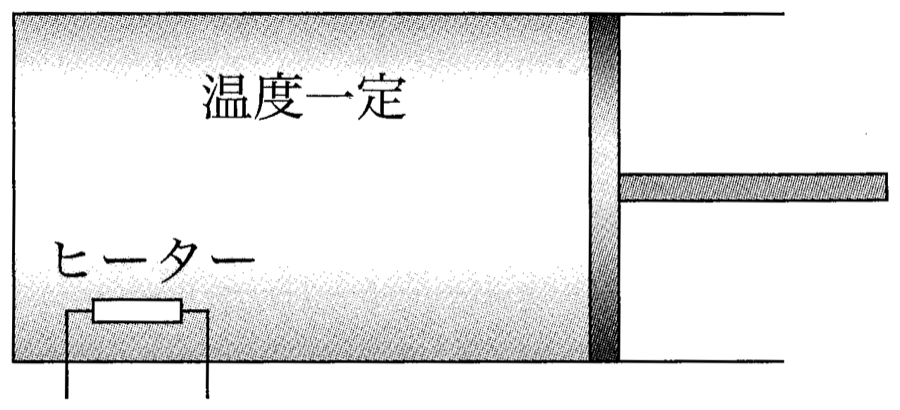
\includegraphics[keepaspectratio,width=58mm]{fig/ch17_ex11_cyl.png}
\end{zuright}
\hspace{1zw}シリンダー内にはヒーターが取り付けてあり，気体に対して熱を与えることができる．シリンダーおよびピストンは断熱材で出来ており，ヒーターによって与えた熱が大気に逃げることはないものとする．気体定数を$R\U{J/mol\cdot K}$として以下の問に答えよ．
\begin{komon}
\ko{1} 始めの状態における気体の圧力$P_0\U{Pa}$を求めよ．
\end{komon}
\hspace{1zw}ここで，気体が温度$T_0\U{K}$を保つようにピストンを操作しながら気体に熱をゆっくりと与え，体積を$V_1\U{m^3}$となるまで膨張させた．
\begin{komon}
\ko{2} 終状態における気体の圧力$P_1\U{Pa}$を求めよ．
\ko{3} 気体の体積が$V\U{m^3}$（$V_0<V<V_1$）のときの気体の圧力$P(V)\U{Pa}$を求めよ．
\ko{4} この状態変化を$P-V$図で表せ．
\ko{5} この変化において気体が外界に対してした仕事$w\U{J}$を求めよ．ただし，$\displaystyle\int\frac{1}{x}dx=\log|x|+C$（$C$は積分定数）である．
\ko{6} この変化における気体の内部エネルギーの増加量$\Delta U\U{J}$を求めよ．
\ko{7} ヒーターによって加えた熱量$Q\U{J}$を求めよ．
\end{komon}
\end{reidai}

\begin{sisinE}
温度が一定に保たれる状態変化を{\gtfamily 等温変化}という．等温変化では内部エネルギーが変化しないので，加えた熱はすべて気体が外界にする仕事になる．

(5) この状態変化では圧力$P$は一定ではないから，$w=P\Delta V$とは書けないことに注意せよ．体積が$V\U{m^3}$のときの圧力$P(V)$を求め，それを積分する．
\end{sisinE}

\Key{状態方程式 $PV=nRT$\quad 内部エネルギー変化 $\Delta U=nC_V\Delta T$\quad 気体のする仕事 $w=\displaystyle\int_{V_1}^{V_2}P\,dV$\quad 熱力学第一法則 $\Delta U=Q+(-w)$}

\begin{kaitou}
\begin{komon}
\ko{1} 始めの状態の状態方程式$P_0V_0=nRT_0$より，
       \Ana{P_0=\frac{nRT_0}{V_0}\U{Pa}\Ans}
\ko{2} 終状態でも温度は$T_0$のままであるから，状態方程式$P_1V_1=nRT_0$より，
       \Ana{P_1=\frac{nRT_0}{V_1}\U{Pa}\Ans}
\ko{3} 体積が$V$のときも温度は$T_0$であるから，状態方程式$P(V)\cdot V=nRT_0$より，
       \Ana{P(V)=\frac{nRT_0}{V}\U{Pa}\Ans}
\ko{4} (3)より$P-V$図は$PV=nRT_0$（一定）の双曲線の一部で，次図の通り．
       \begin{center}
       \ifbsAnaume
       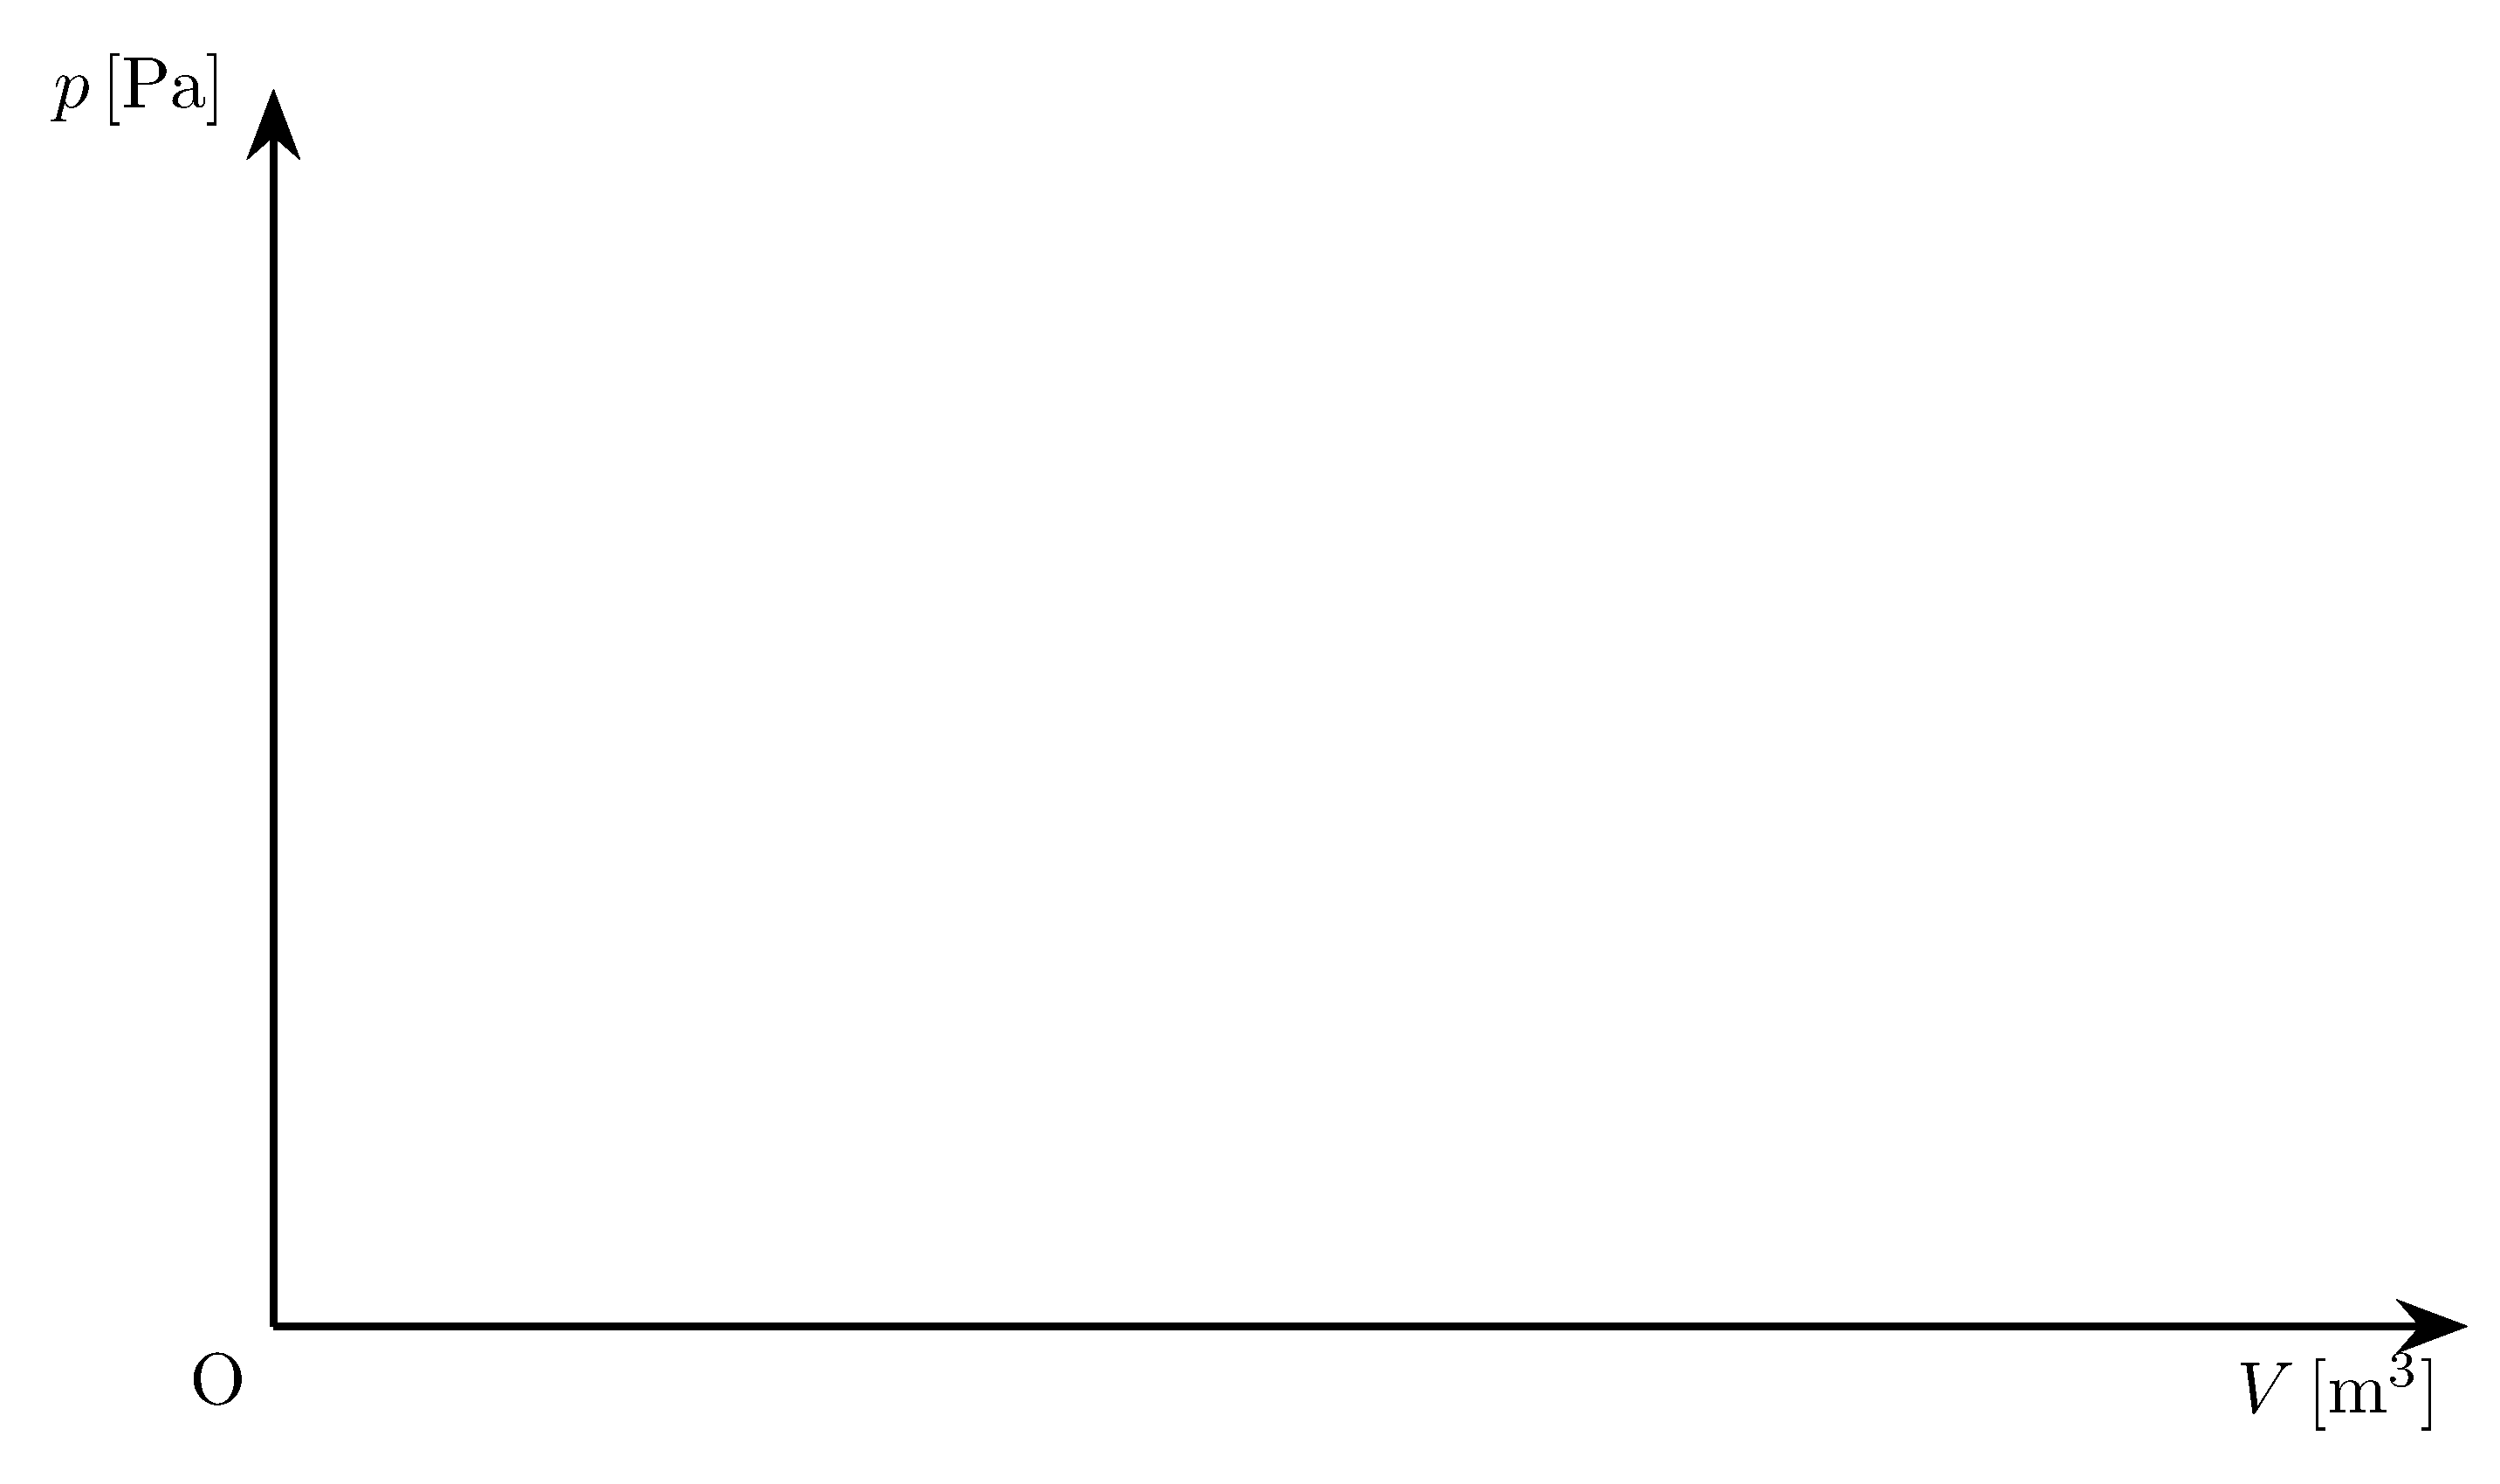
\includegraphics[keepaspectratio,width=96mm]{fig/ch17_ex11_pv_blank.png}
       \else
       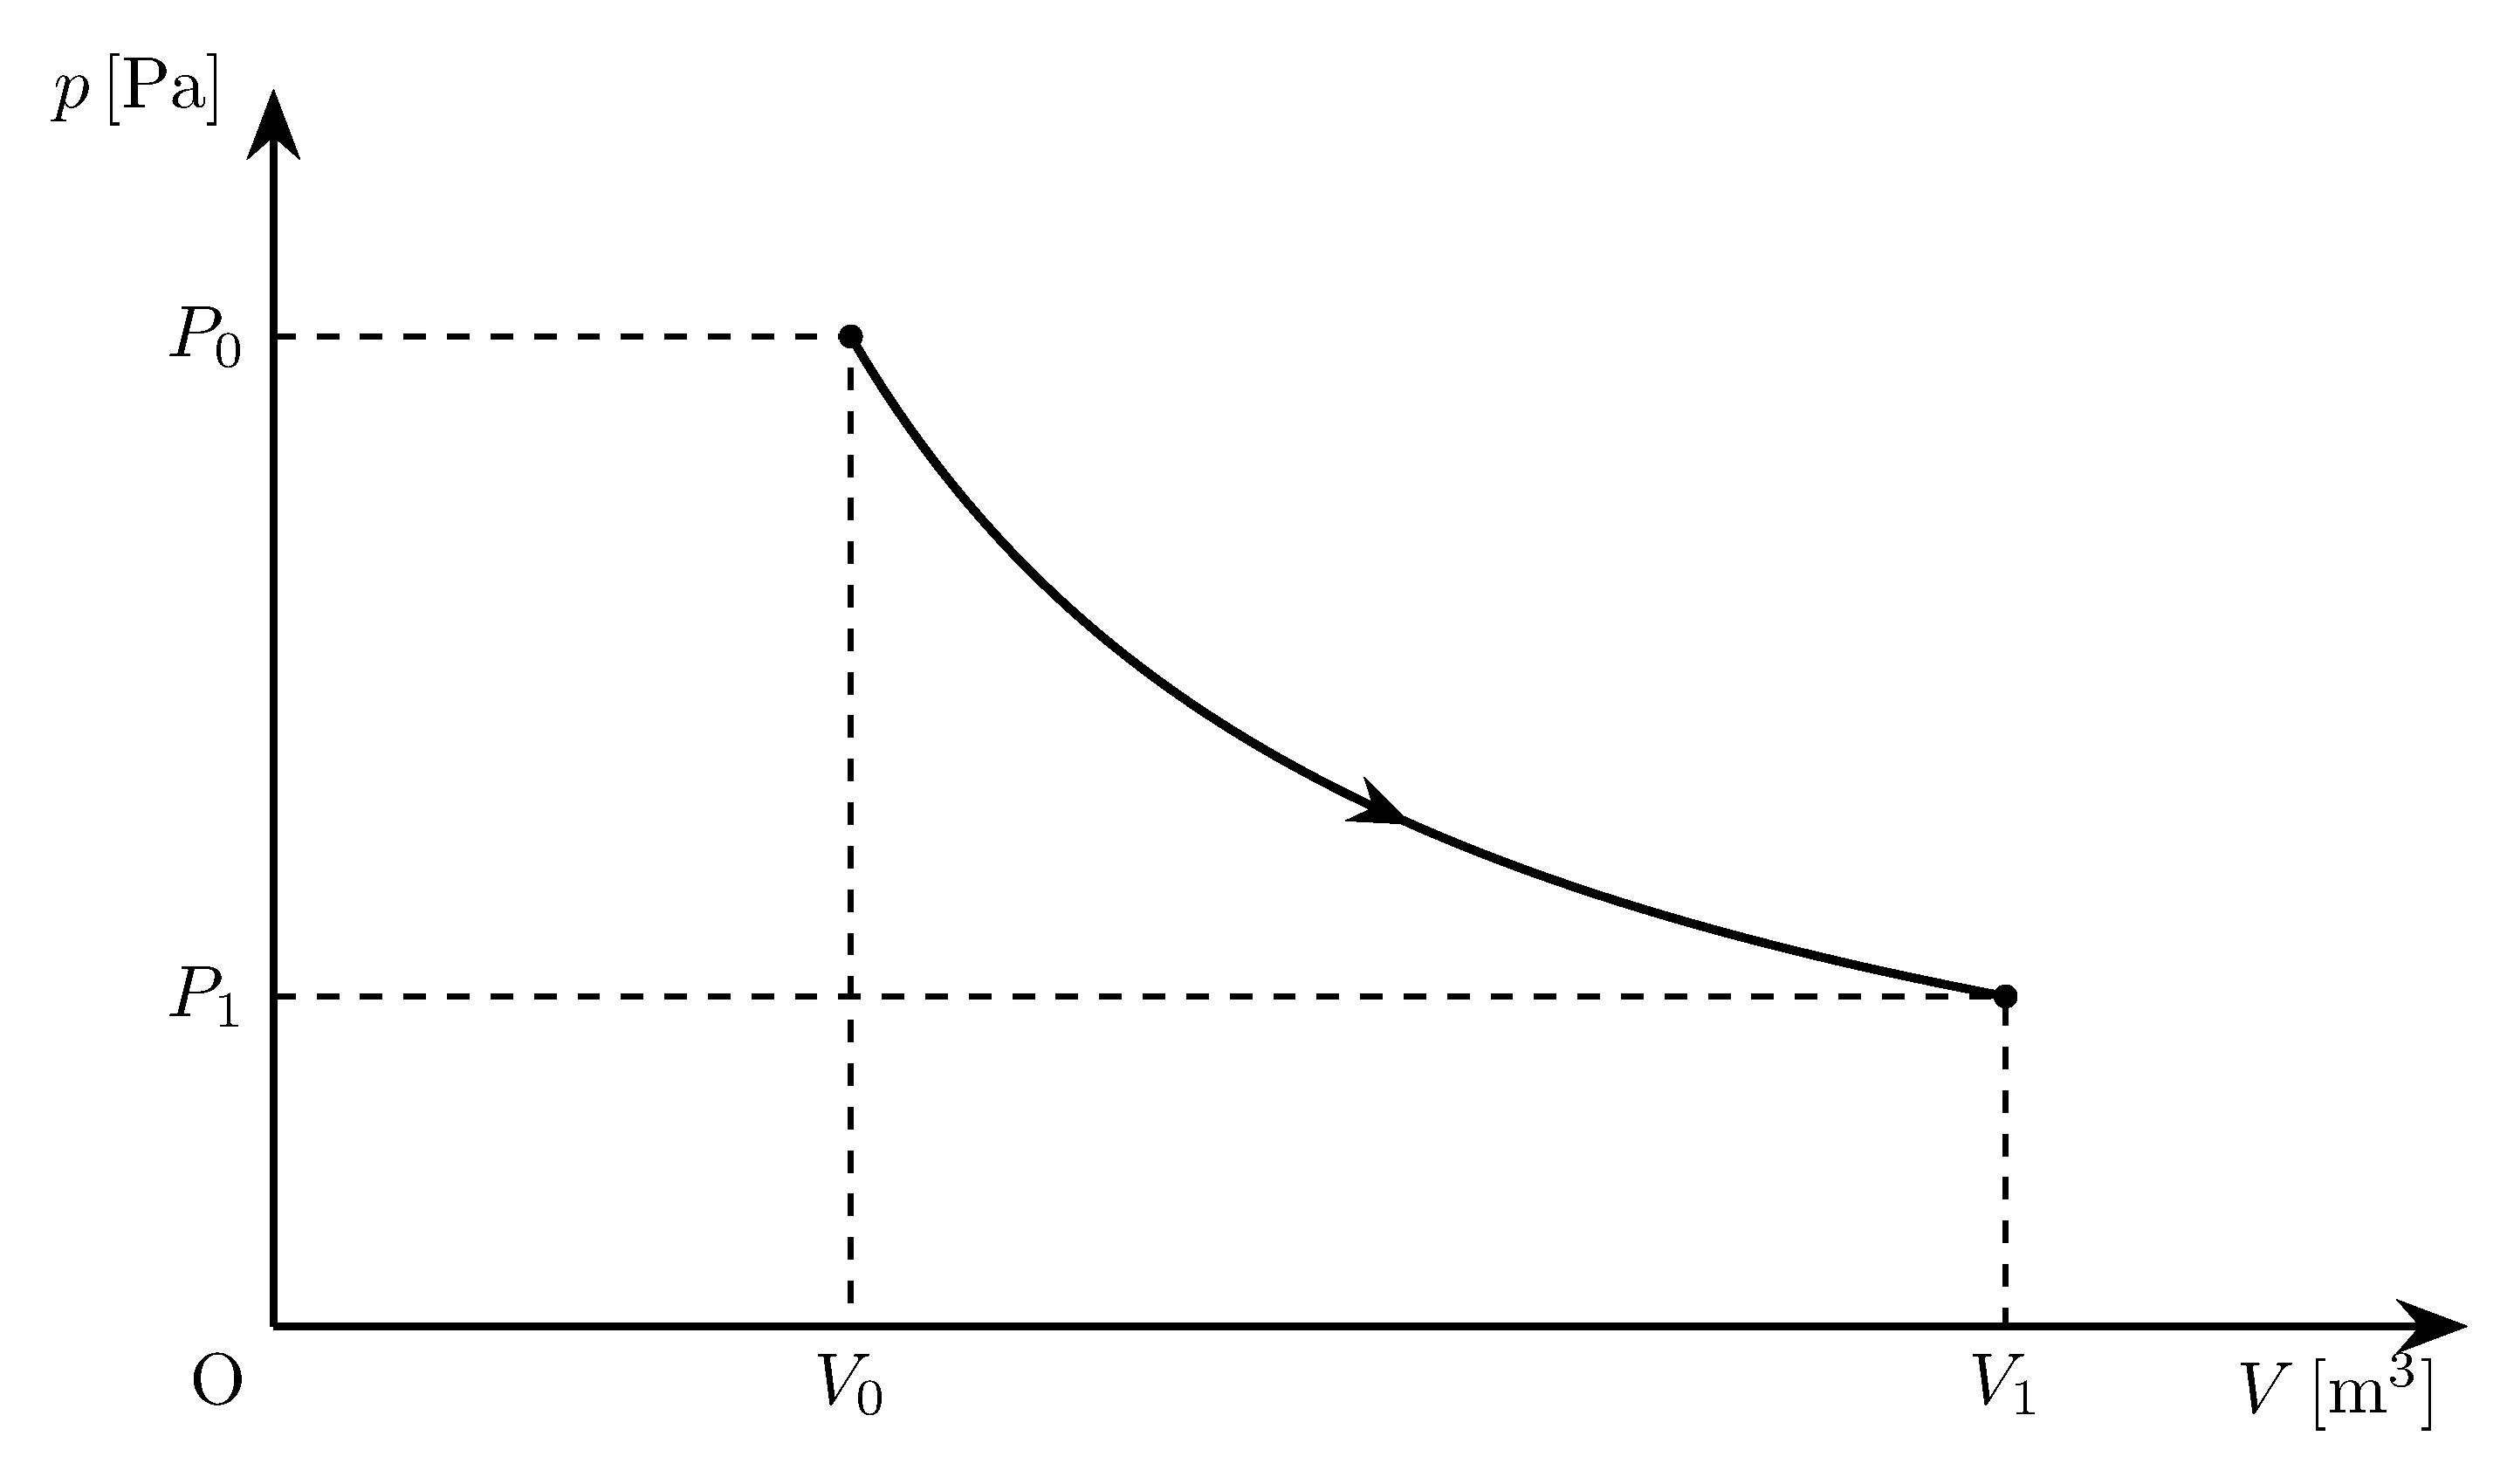
\includegraphics[keepaspectratio,width=96mm]{fig/ch17_ex11_pv.png}
       \fi
       \end{center}
       \hspace*{\fill}\Ans
\ko{5} $nRT_0$は定数であることに注意して，
       \Ana{w=\int_{V_0}^{V_1}P(V)dV=nRT_0\int_{V_0}^{V_1}\frac{1}{V}dV
             =nRT_0\log_e\frac{V_1}{V_0}\U{J}\Ans}
\ko{6} 温度が$T_0$のまま変化しないので$\Delta T=0$であり，
       \Ana{\Delta U=nC_V\Delta T=0\U{J}\Ans}
\ko{7} 熱力学第一法則$\Delta U=Q+(-w)$より，
       \Ana{Q=\Delta U+w=nRT_0\log_e\frac{V_1}{V_0}\U{J}\Ans}
       すなわち，加えた熱はすべて気体が外界にした仕事になっている．
\end{komon}
\end{kaitou}
\end{reidaiunit}


\subsection{断熱変化}
外部との熱の出入りを遮断して気体を状態変化させることを断熱変化という．
断熱変化では圧力，体積，温度の全てが変化する．

\begin{reidaiunit}
\begin{reidai}{断熱変化}
\hspace{1zw}始状態において圧力$P_0\U{Pa}$，体積$V_0\U{m^3}$の理想気体を，外部との熱のやり取りを断ったまま体積が$V_1\U{m^3}$（ただし$V_1>V_0$）になるまで変化させる．終状態における気体の圧力を$P_1\U{Pa}$，気体定数を$R\U{J/mol\cdot K}$，気体の定積モル比熱を$C_V\U{J/mol\cdot K}$として以下の問に答えよ．
\begin{komon}
\ko{1} 内部エネルギー変化$\Delta U\U{J}$，気体が外にした仕事$w\U{J}$，吸熱量$Q\U{J}$を求めよ．
\ko{2} 膨張過程なので$w>0$である事を利用して，この変化によって気体の温度は増加するか，減少するか，答えよ．
\end{komon}
\end{reidai}

\begin{sisinE}
熱の出入りを断った状態変化なので$Q=0$である．与えられているのは$P$と$V$だけで温度が与えられていないが，状態方程式$PV=nRT$を使えば$nRT$を$PV$に置き換えられるので，$\Delta U=nC_V\Delta T$は$P$, $V$だけで表せる．
\end{sisinE}

\begin{kaitou}
\begin{komon}
\ko{1} 断熱変化であるから，
       \[Q=0\U{J}\Ans\]
       気体のモル数を$n\U{mol}$，始状態・終状態の温度を$T_0\U{K}$, $T_1\U{K}$とすると，状態方程式より$P_0V_0=nRT_0$, $P_1V_1=nRT_1$であるから，
       \[\Delta U=nC_V(T_1-T_0)=\frac{C_V}{R}(P_1V_1-P_0V_0)\U{J}\Ans\]
       熱力学第一法則$\Delta U=Q+(-w)$に$Q=0$を代入して，
       \Ana{w=-\Delta U=\frac{C_V}{R}(P_0V_0-P_1V_1)\U{J}\Ans}
\ko{2} (1)より$\Delta U=-w$であり，$w>0$であるから$\Delta U<0$である．$\Delta U=nC_V\Delta T$で$nC_V>0$であるから$\Delta T<0$，すなわち気体の温度は\AnaU{\gtfamily 減少する}．\hspace*{\fill}\Ans
\end{komon}
\end{kaitou}
\end{reidaiunit}

% 加筆（2026-09-02）：原本 p79 の例題12 の直後の段落．例題12 を入れたので，
%   ポアソンの法則へつなぐ原本どおりの言い回しに戻した．
準静的な断熱変化では圧力，体積，温度の全てが変化するが，終状態は1通りしか取れないため，例題12の終状態の圧力$P_1$[Pa]は与えられた文字を用いて表すことが出来るはずである．
この値を求めるためには以下に示す{\bf ポアソンの法則}を利用する．

\begin{matome}{ポアソンの法則}
 \hspace{3mm} 断熱変化中は比熱比$\gamma =\dfrac{C_P}{C_V}$を用いて
 \[PV^\gamma =（一定）　TV^{\gamma-1}=（一定）\]
 が成立する．
 \end{matome}

この法則を微小変化に注目して導出してみよう．

\begin{wrapfigure}[17]{r}[5mm]{60mm}
  \centering
  \vspace{-5mm}
  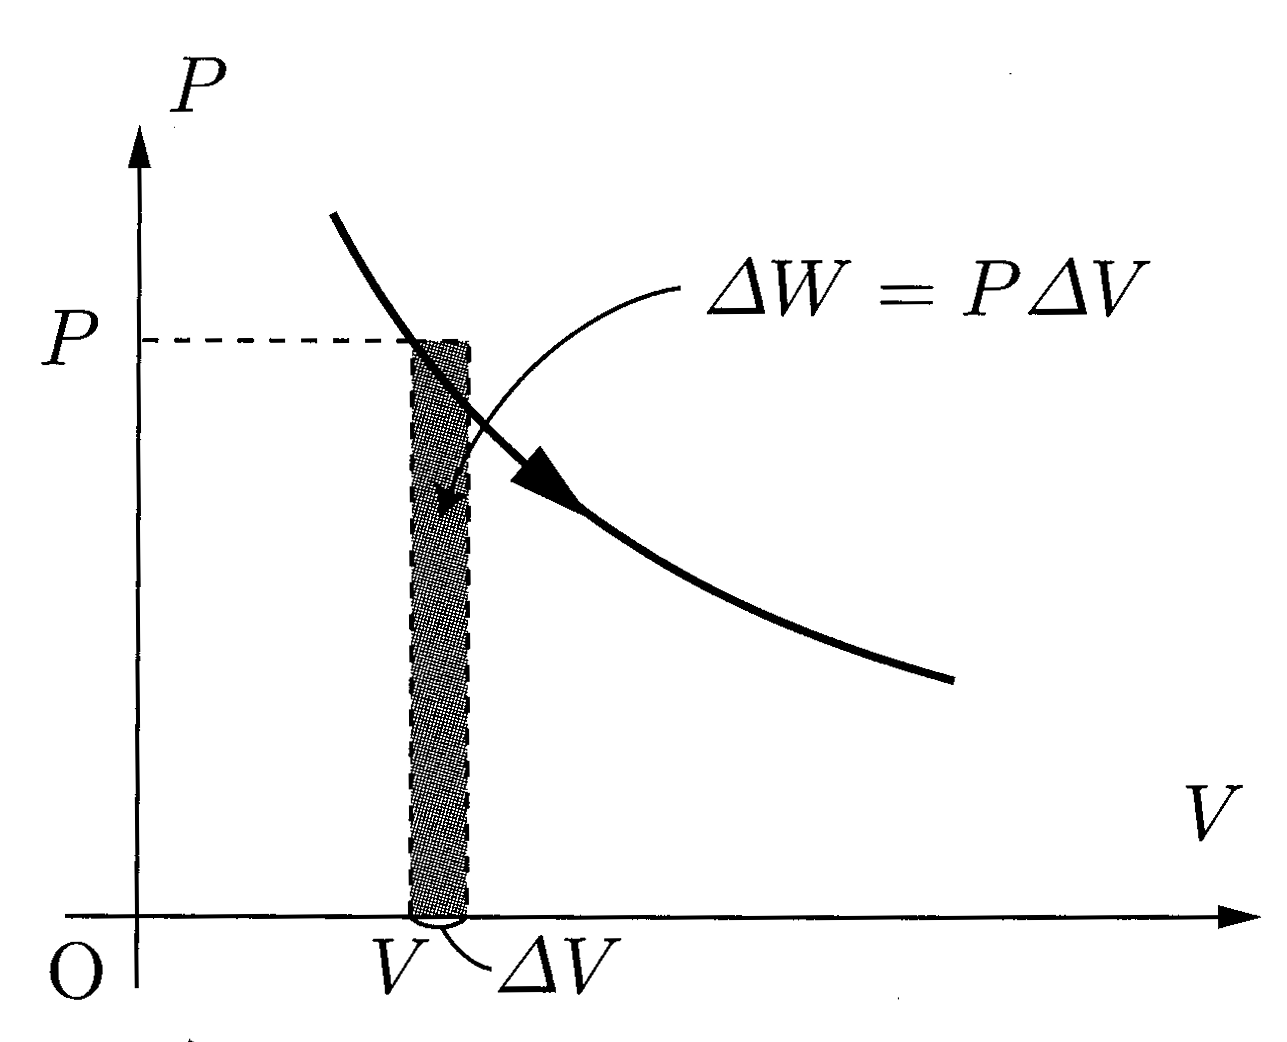
\includegraphics[keepaspectratio,width=60mm]
  {text_p79_fig1.png}
\end{wrapfigure}
体積$V[{\rm m^3}]$のときの圧力を$P$[Pa]として，微小体積$\Delta V[{\rm m^3}]$分の気体を断熱膨張させると，この間に気体が外にした微小仕事は
\[\Delta W=P\Delta V\]
となる．
この変化の前後で圧力が$\Delta P$[Pa]，温度が$\Delta T$[K]だけ変化したとすると，断熱変化なので，熱力学第一法則より，
\[0=nC_V\Delta T+\Delta W \hspace{5mm} \Leftrightarrow \hspace{5mm} nC_V\Delta T=-P\Delta V\]

ここで，断熱膨張前後の状態方程式より
\[PV=nRT\]
\[(P+\Delta P)(V+\Delta V)=nR(T+\Delta T)\]

第2式において二次の微小量$\Delta P\Delta V$を無視して第1式を利用すれば
\[PV+P\Delta V +\Delta PV=nRT+nR\Delta T\]
\[\Leftrightarrow P\Delta V +\Delta PV=nR\Delta T\]
熱力学第一法則の式に代入して
\[\dfrac{C_V}{R}(P\Delta V+\Delta PV)=-P\Delta V \hspace{5mm} \Leftrightarrow \hspace{5mm} \dfrac{C_V+R}{C_V}・\dfrac{\Delta V}{V}=-\dfrac{\Delta P}{P}\]

マイヤーの関係式より$C_P=C_V+R$なので，$\dfrac{C_V+R}{C_V}=\gamma$と置き換えられる．
これを両辺積分すると，積分定数を$D$として
\[\gamma \log V=-\log P+D \hspace{5mm} \Leftrightarrow \hspace{5mm} \log PV^\gamma =D \hspace{5mm} \Leftrightarrow \hspace{5mm} PV^\gamma =e^D\]

$e^D$は定数なので，$PV^\gamma =（一定）$が成立する．

また，$PV^\gamma =（一定）$と状態方程式$PV=nRT$を合わせて
\[\dfrac{nRT}{V}V^\gamma =（一定）\hspace{5mm} \Leftrightarrow \hspace{5mm} TV^{\gamma -1}=（一定）\]
も示すことができる．

% レイアウト修正（2026-09-02）：ここは wrapfigure[5] だったが，直後の本文が4行しか
%   無いため折り返しが例題13のユニット（1.2pt 全幅罫）に食い込んでいた．
%   段抜けしない zuright（minipage 2段）に置き換えた．
\begin{zuright}{56mm}
\hspace{1zw}等温変化では，状態方程式より$PV=（一定）$が成立するので，等温変化と断熱変化を比較すると，変化中の$P-V$図の曲線（それぞれ等温曲線，断熱曲線と呼ぶ）は{\bf 断熱曲線の方が等温曲線より傾きが大きい}曲線となることがわかる．
\zusep
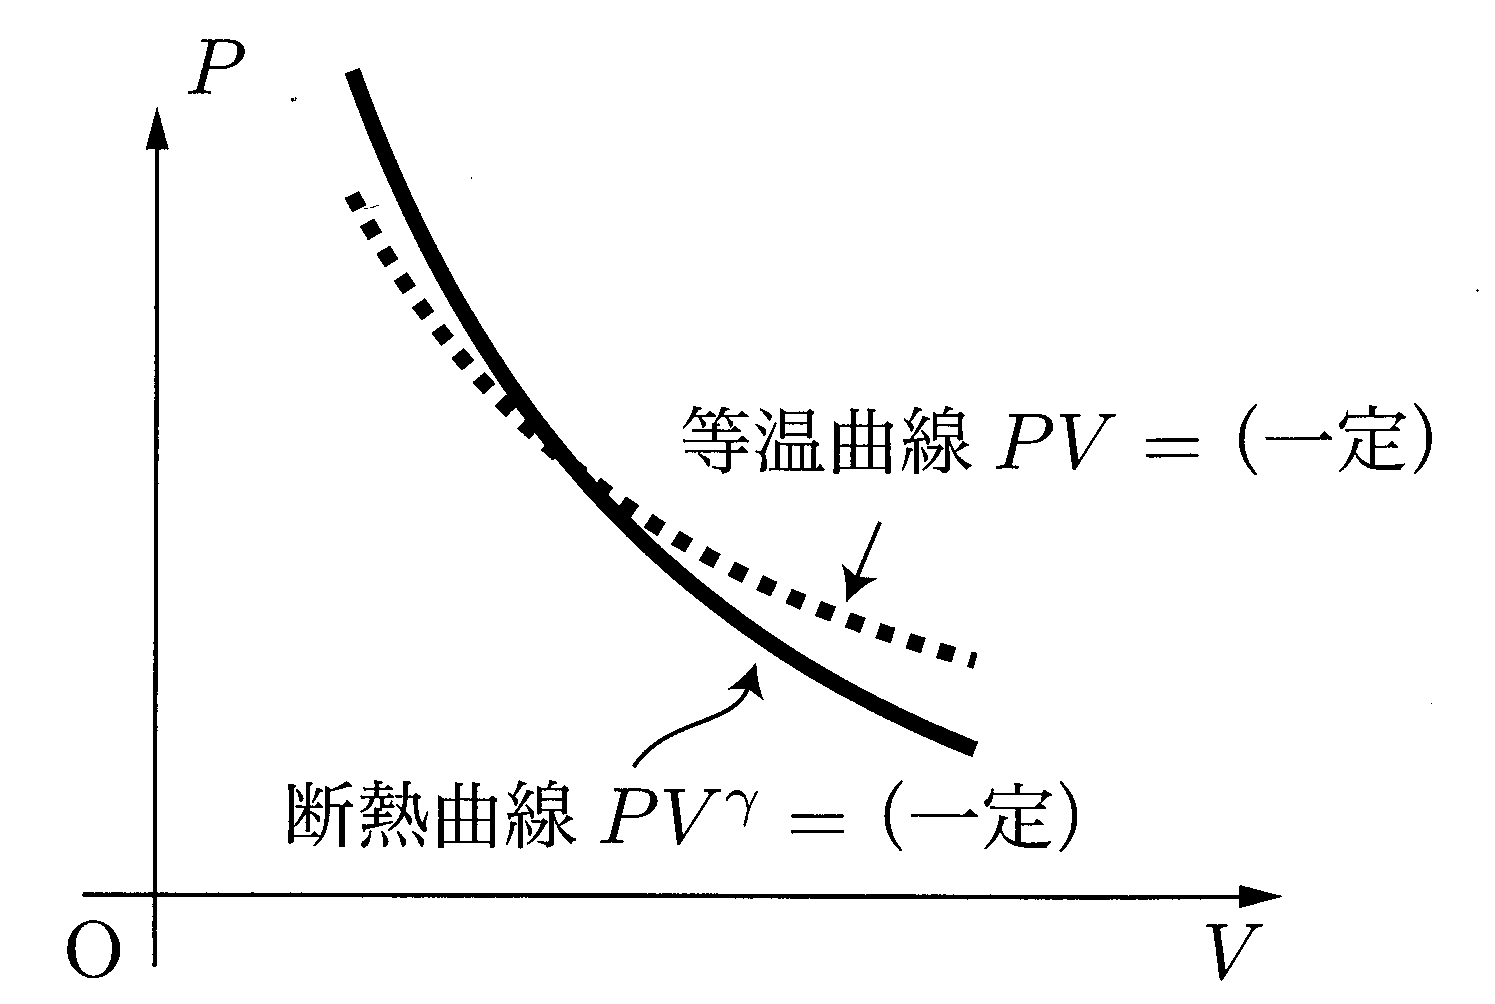
\includegraphics[keepaspectratio,width=56mm]{text_p80_fig1.png}
\end{zuright}

\begin{reidaiunit}
\begin{reidai}{ポアソンの式の利用}
\begin{zuright}{50mm}
\hspace{1zw}図のように一様な断面積を持つシリンダーに定積モル比熱が$C_V\U{J/mol\cdot K}$の理想気体を$n\U{mol}$封入した．ピストンは軽くて自由に動くことができ，外気圧とシリンダー内の気体の圧力とが常につり合いを保つ．シリンダーおよびピストンは断熱材で出来ており，外界との熱のやり取りはない．最初，この気体の温度は$T_0\U{K}$，体積は$V_0\U{m^3}$であり，ピストンは静止していた．
\zusep
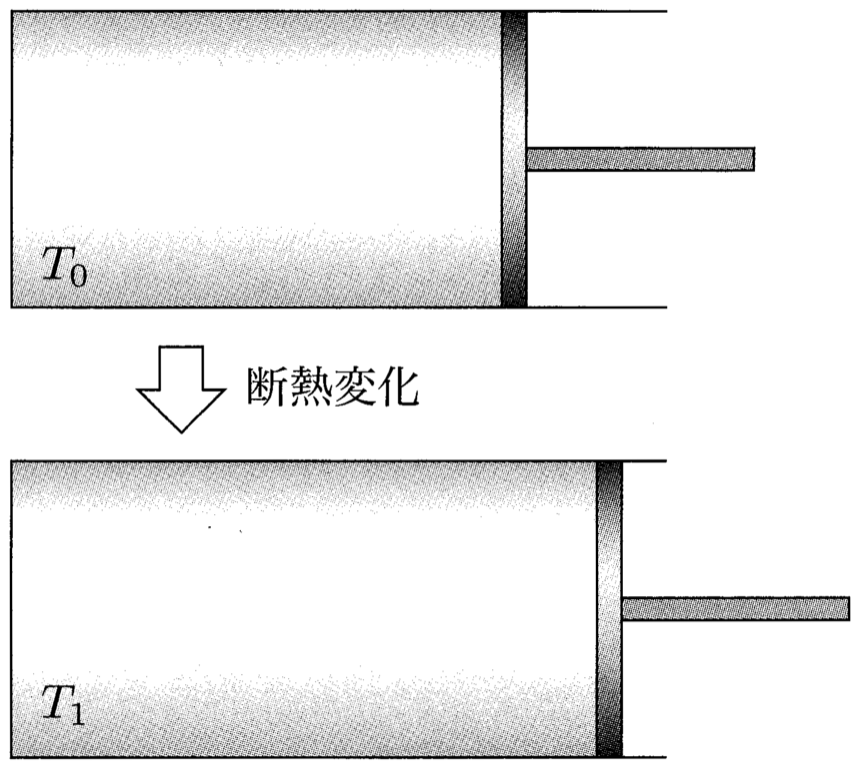
\includegraphics[keepaspectratio,width=50mm]{fig/ch17_ex13_cyl.png}
\end{zuright}
\hspace{1zw}この状態から外気圧をゆっくりと変化させ，気体の温度が$T_1\U{K}$($<T_0$)となるまで変化させた．理想気体が断熱変化するときは比熱比を$\gamma$として，ポアソンの式$PV^\gamma=（一定）$が成立することを用いてよい．気体定数を$R\U{J/mol\cdot K}$として以下の問に答えよ．
\begin{komon}
\ko{1} この状態変化を$P-V$図で表せ．ただし，終状態の体積を$V_1\U{m^3}$として図示せよ．
\ko{2} この気体が始状態から定温条件で体積$V_1\U{m^3}$となるまで変化した場合，気体はどのような曲線上を動くか．(1)の$P-V$図に点線で記入せよ．
\ko{3} この気体の内部エネルギー変化$\Delta U\U{J}$を求めよ．
\ko{4} この気体が外界にした仕事$w\U{J}$を求めよ．
\ko{5} 終状態における気体の体積$V_1\U{m^3}$を求めよ．
\end{komon}
\end{reidai}

\begin{sisinE}
温度が下がる断熱変化であるから，気体は外界に仕事をして膨張する（$V_1>V_0$）．$P-V$図では断熱曲線は等温曲線より急な右下がりの曲線になるので，同じ体積$V_1$まで変化させたとき断熱変化の方が圧力は低い．

断熱変化では$Q=0$なので，仕事$w$は積分せずとも熱力学第一法則$\Delta U=Q+(-w)$から求まる．体積を問われている(5)では，$P$と$V$を結ぶ$PV^\gamma=（一定）$ではなく$T$と$V$を結ぶ$TV^{\gamma-1}=（一定）$を使う．
\end{sisinE}

\Key{断熱変化中は比熱比$\gamma=\dfrac{C_P}{C_V}$を用いて $PV^\gamma=（一定）$, $TV^{\gamma-1}=（一定）$ が成立する}

\begin{kaitou}
\begin{komon}
\item[{\makebox[1.9zw][r]{(1)(2)}}] 断熱変化（実線）は$PV^\gamma=（一定）$，等温変化（点線）は$PV=（一定）$の曲線である．$\gamma>1$であるから断熱曲線の方が急になり，次図の通り．
       \begin{center}
       \ifbsAnaume
       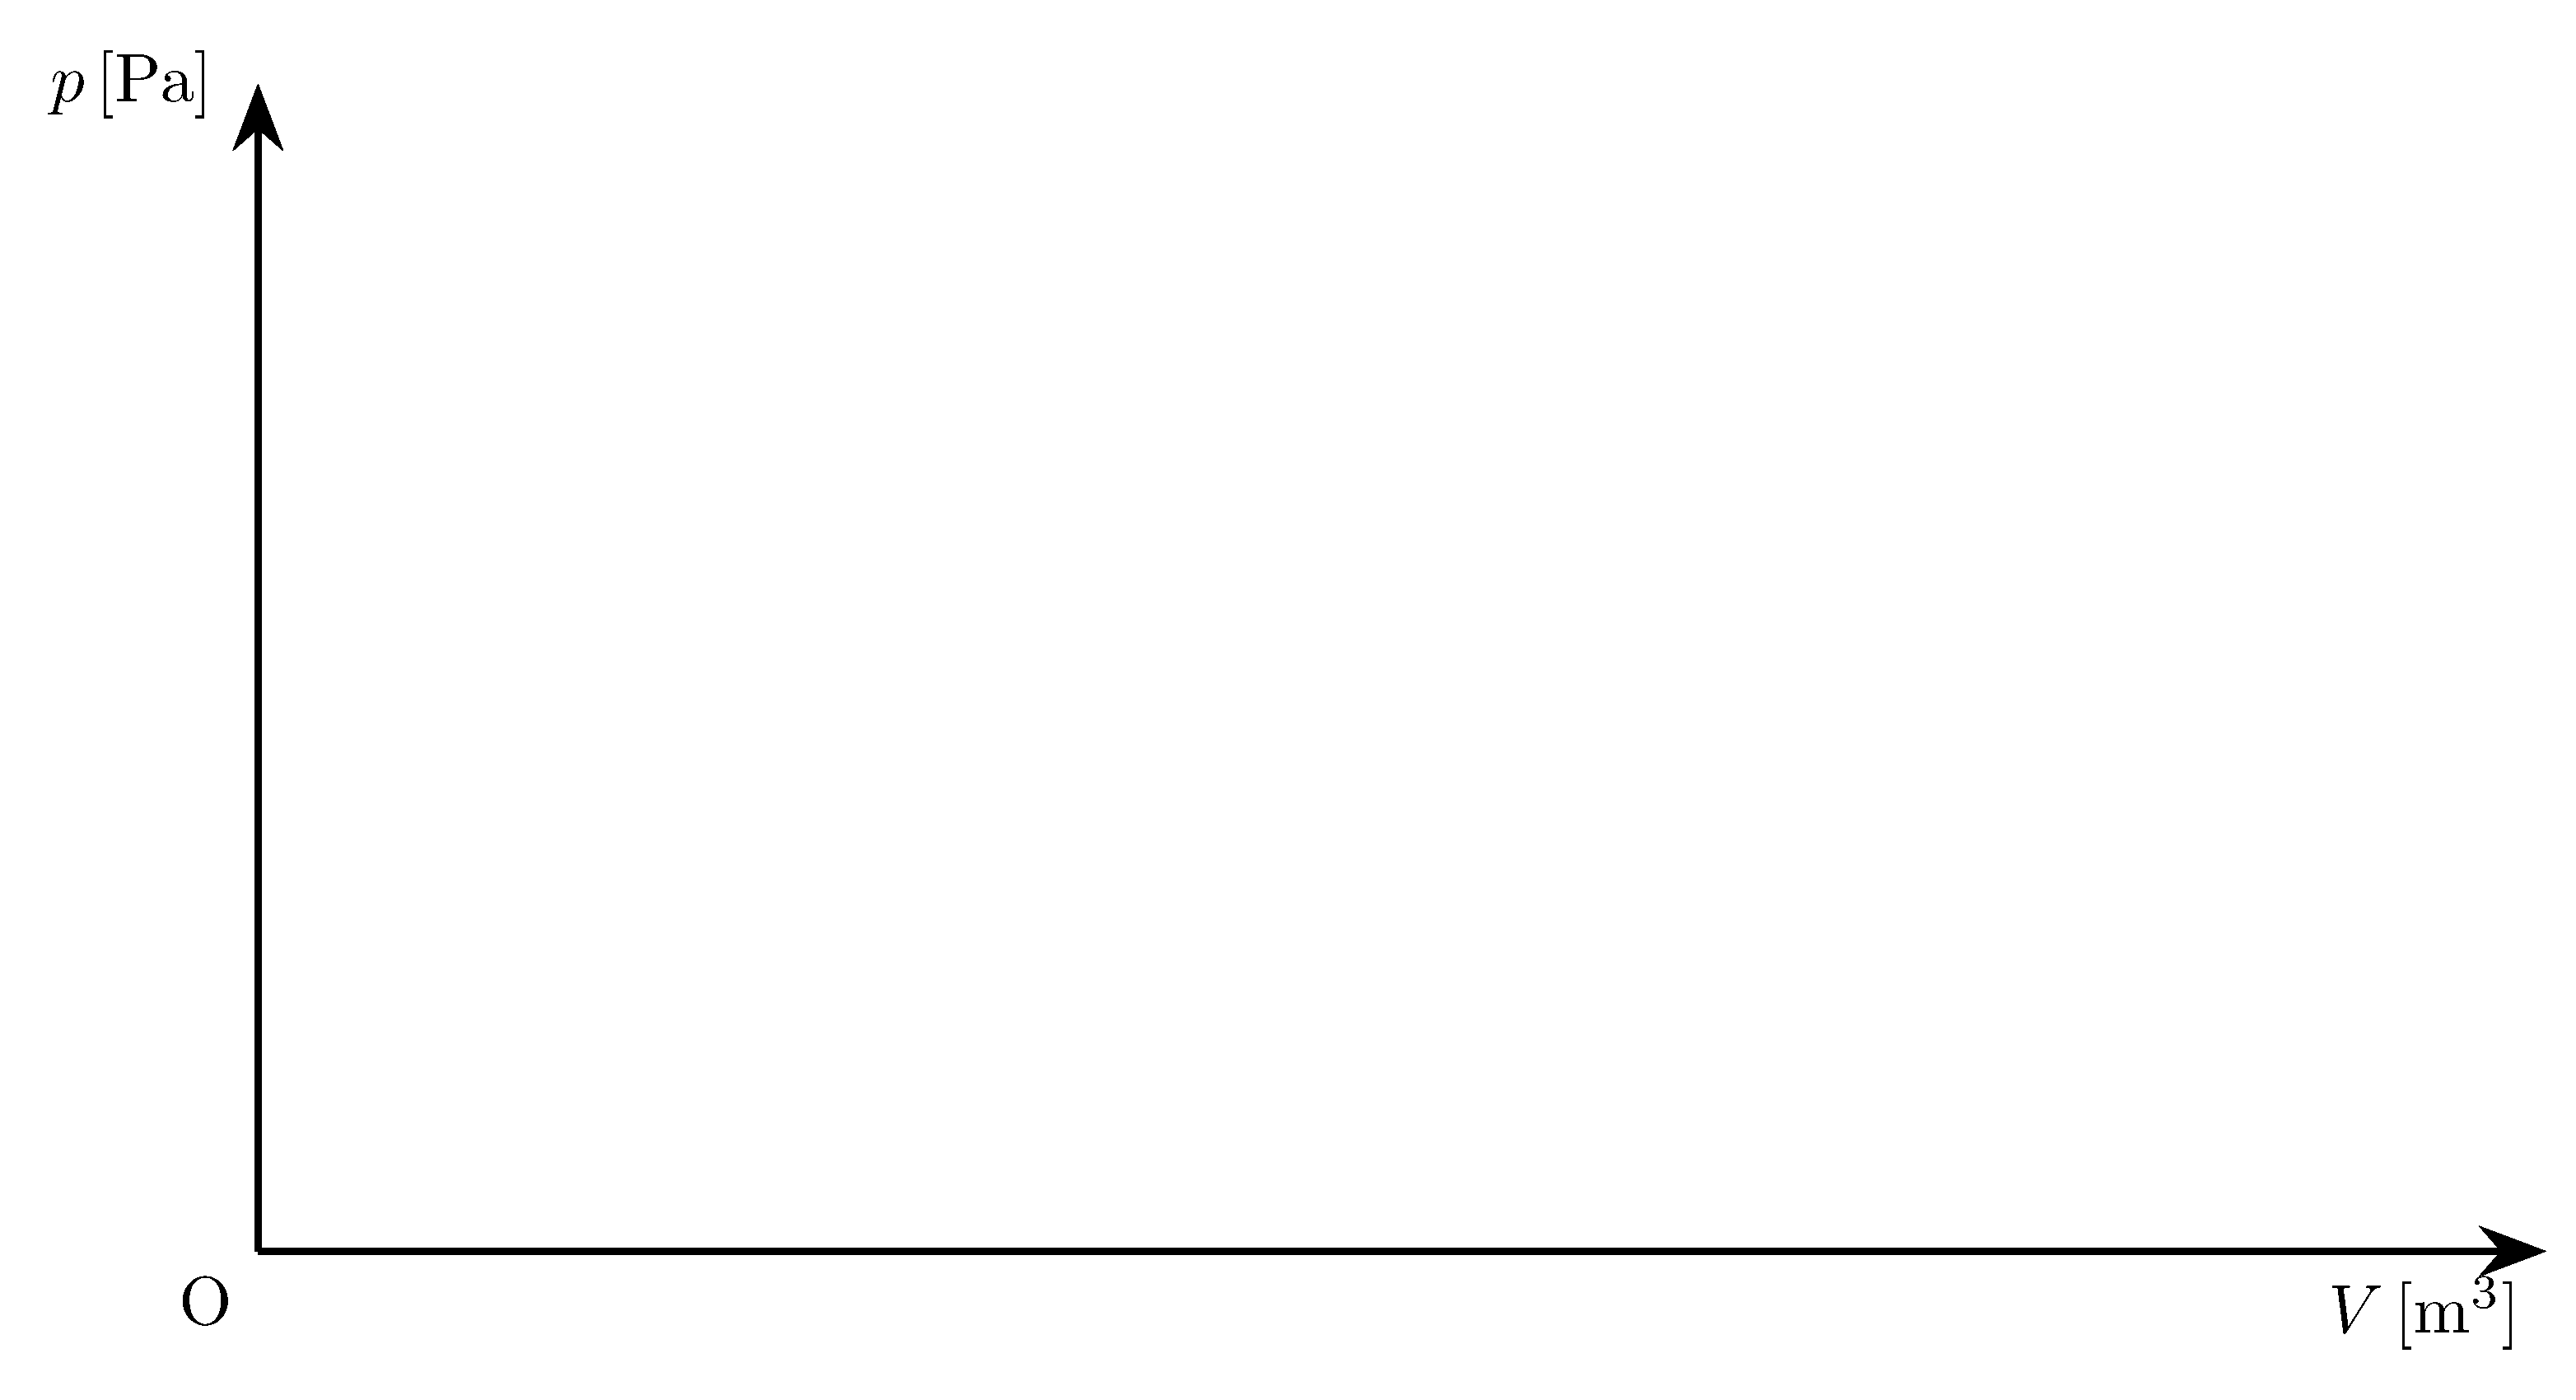
\includegraphics[keepaspectratio,width=106mm]{fig/ch17_ex13_pv_blank.png}
       \else
       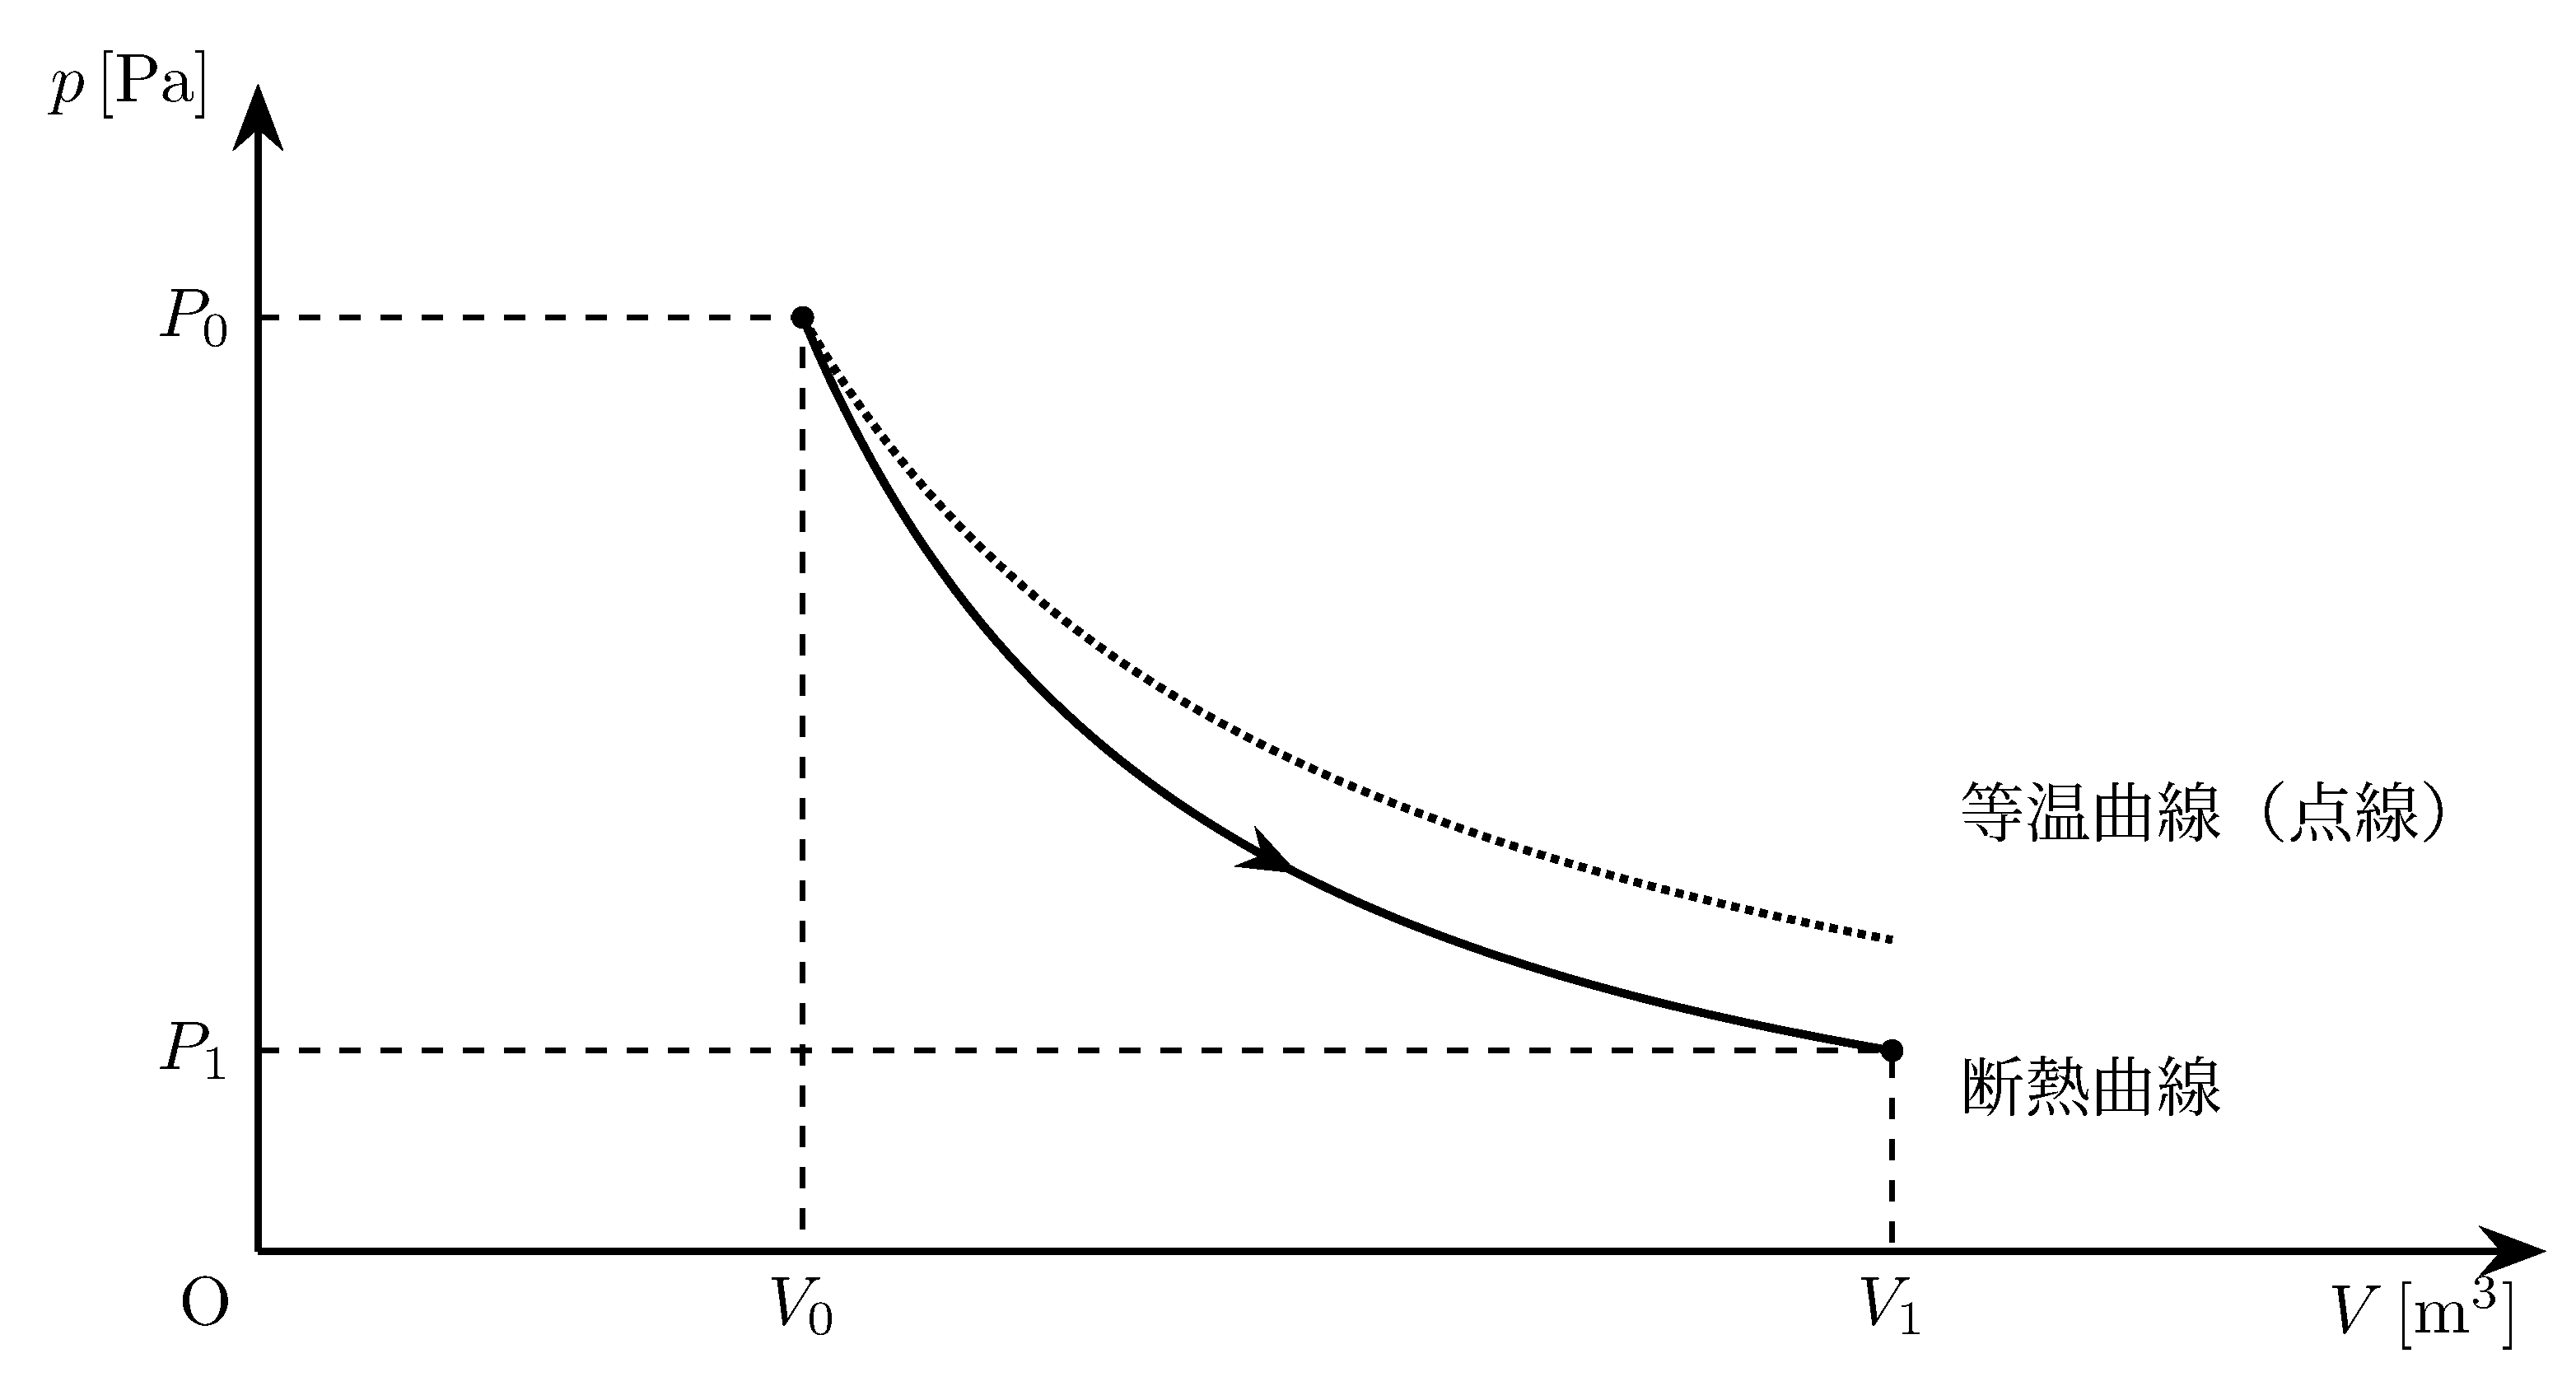
\includegraphics[keepaspectratio,width=106mm]{fig/ch17_ex13_pv.png}
       \fi
       \end{center}
       \hspace*{\fill}\Ans
\ko{3} 内部エネルギーは絶対温度だけで決まるので，
       \Ana{\Delta U=nC_V(T_1-T_0)\U{J}\Ans}
       $T_1<T_0$であるから$\Delta U<0$，すなわち内部エネルギーは減少する．
\ko{4} 断熱変化であるから$Q=0$であり，熱力学第一法則$\Delta U=Q+(-w)$より，
       \Ana{w=-\Delta U=nC_V(T_0-T_1)\U{J}\Ans}
\ko{5} マイヤーの関係式$C_P=C_V+R$より$\gamma-1=\dfrac{C_P}{C_V}-1=\dfrac{R}{C_V}$である．ポアソンの式\mbox{$TV^{\gamma-1}=（一定）$}を始状態と終状態に適用して，
       \[T_0V_0^{\gamma-1}=T_1V_1^{\gamma-1}\]
       これを$V_1$について解くと，
       \Ana{V_1=V_0\left(\frac{T_0}{T_1}\right)^{\frac{1}{\gamma-1}}
             =V_0\left(\frac{T_0}{T_1}\right)^{\frac{C_V}{R}}\U{m^3}\Ans}
       $T_0>T_1$であるから$V_1>V_0$となり，膨張していることが確かめられる．
\end{komon}
\end{kaitou}
\end{reidaiunit}


\subsection{自由膨張}
% 加筆（2026-09-02）：原本 p81 は「次の例題のように，」で始まり，例題14 を指している．
%   例題14 を原本と同じ位置（まとめ枠の直後）に入れたので，この言い回しを戻した．
次の例題のように，気体が真空中に拡散していく際には，左右の部屋の圧力が異なる状態を経て気体が真空側へと流れていき，最終的には両方の部屋の気体の圧力が等しくなったところで気体の流れが止まる．
このような真空中への気体の膨張を{\bf 自由膨張}といい，特に熱を遮断した状態で真空中へ膨張させることを{\bf 断熱自由膨張}という．

断熱自由膨張では，もともと気体の入っていた部屋から気体が出ていき，片方の部屋に注目すると気体のモル数が変化していくため，準静的な断熱変化で議論した場合と異なる．
そのため，断熱変化ではあるものの，ポアソンの式$PV^\gamma=（一定）$を用いて考えてはいけない．
このような場合は，箱全体に着目し熱力学第一法則を適用する．箱全体の体積は変わらず，また断熱変化なら箱の内外の熱のやりとりが0[J]である．
よって，箱内部の内部エネルギー変化が0[J]となることがわかる．

\begin{matome}{断熱自由膨張}
 \hspace{3mm} 熱を遮断した状態で真空中へ理想気体を膨張させるときは箱全体に対して熱力学第一法則を考える．
 \end{matome}

\begin{reidaiunit}
\begin{reidai}{断熱自由膨張}
\begin{zuright}{52mm}
\hspace{1zw}断熱材で作られた容器の中に，仕切板を隔てて図の左側の空間にのみ定積モル比熱が$C_V\U{J/mol\cdot K}$，温度が$T_0\U{K}$の理想気体が$n\U{mol}$封入されている．
\zusep
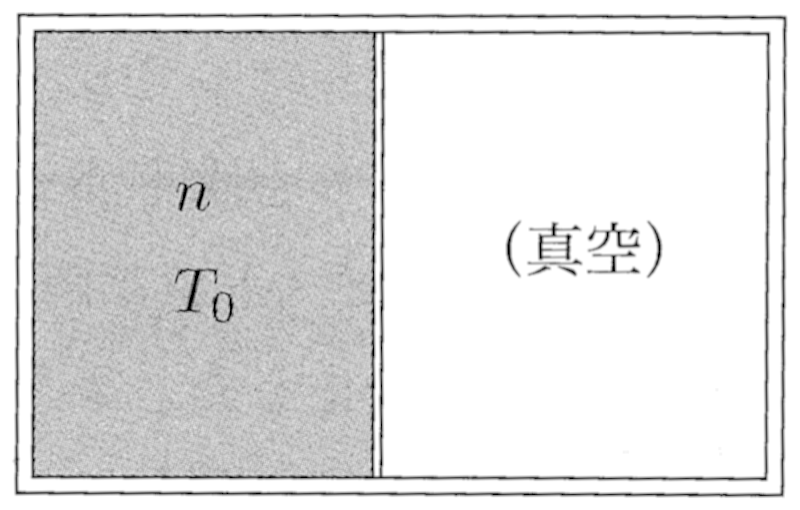
\includegraphics[keepaspectratio,width=52mm]{fig/ch17_ex14_box1.png}
\end{zuright}
\begin{komon}
\ko{1} この仕切板に穴を開けると気体は右側へと拡散していく．十分時間がたったのちの気体の温度$T^\prime\U{K}$を求めよ．
\end{komon}
\begin{zuright}{52mm}
\hspace{1zw}先と同じく断熱材で作られた容器の中に，仕切板を隔てて図のように左側，右側それぞれに異なる気体を封入する．左側（体積$V_1\U{m^3}$）には定積モル比熱$C_{V1}\U{J/mol\cdot K}$，温度が$T_1\U{K}$の理想気体が$n_1\U{mol}$だけ封入されており，右側（体積$V_2\U{m^3}$）には定積モル比熱$C_{V2}\U{J/mol\cdot K}$，温度が$T_2\U{K}$の理想気体が$n_2\U{mol}$だけ封入されている．
\zusep
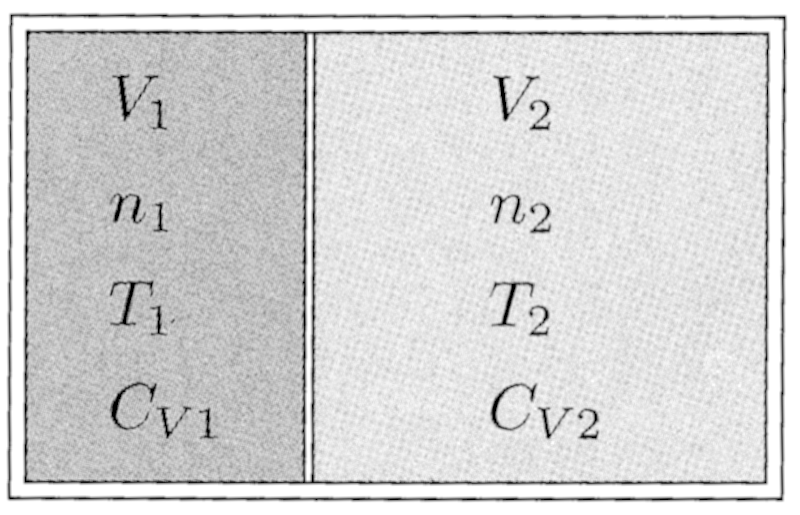
\includegraphics[keepaspectratio,width=52mm]{fig/ch17_ex14_box2.png}
\end{zuright}
\begin{komon}
\ko{2} この仕切板を取り外し，外界との熱のやり取りを断って2つの気体を混合する．十分時間がたったのちの温度$T\U{K}$を求めよ．
\end{komon}
\end{reidai}

\begin{sisinE}
どちらも{\gtfamily 容器全体を一つの系とみなして熱力学第一法則を立てる}．容器の体積は変わらないので外界と仕事のやり取りはなく（$W=0$），断熱材で作られているので熱のやり取りもない（$Q=0$）．したがって容器全体の内部エネルギーの変化は$\Delta U=0$である．

(2)では，容器全体の内部エネルギー変化は左側の気体の変化と右側の気体の変化の和であることを使う．
\end{sisinE}

\Key{真空中への断熱自由膨張 $\Rightarrow$ 箱全体に対しての熱力学第一法則}

\begin{kaitou}
\begin{komon}
\ko{1} 容器全体を一つの系とみなすと，体積が変わらないので$W=0$，断熱材なので$Q=0$である．よって熱力学第一法則より
       \[\Delta U=Q+W=0\]
       一方，内部エネルギーの変化は$\Delta U=nC_V(T^\prime-T_0)$と表せるから，$nC_V\neq 0$より$T^\prime-T_0=0$，すなわち
       \Ana{T^\prime=T_0\U{K}\Ans}
\ko{2} こちらも容器全体では$Q=0$, $W=0$であるから$\Delta U=0$である．混合後の温度を$T\U{K}$とすると，左側の気体の内部エネルギー変化と右側の気体の内部エネルギー変化の和が$\Delta U$であるから，
       \[n_1C_{V1}(T-T_1)+n_2C_{V2}(T-T_2)=0\]
       これを$T$について解いて，
       \Ana{T=\frac{n_1C_{V1}T_1+n_2C_{V2}T_2}{n_1C_{V1}+n_2C_{V2}}\U{K}\Ans}
\end{komon}
\end{kaitou}
\end{reidaiunit}



\newpage

%%%%%%%%%%%%%%%%%%%%  練習問題（旧 prob_p43.png / prob_p44.png / prob_p45.png）  %%%%%%%%%%%%%%%%%%%%
% 第16回の［23］に続く．章単体で組んだときも番号が本体と一致するように明示しておく
\setcounter{qno}{23}

\filbreak
\Rank{A問題}

\Mon{基本事項の確認}

\hspace{1zw}以下の設問に答えよ．

\hspace{1zw}単原子分子理想気体，二原子分子理想気体の定積モル比熱はそれぞれ$\dfrac{3}{2}R$, $\dfrac{5}{2}R$である．このときそれぞれの比熱比はいくらか．

\filbreak
\Rank{B問題}

\Mon{状態変化に伴う各物理量の変化}

\hspace{1zw}ピストンのついた容器の中に一定量の気体を入れ，次の各変化を行う場合，\MARU{1}\MARU{2}\MARU{3}\MARU{4}に適するものを選べ．
\begin{komon}
\ko{1} 圧力を一定に保って圧縮させるとき
\ko{2} 体積を一定に保って減圧するとき
\ko{3} 温度を一定に保って加圧するとき
\ko{4} 外界との熱のやり取りを断ち切って圧縮するとき
\end{komon}
\hspace{1zw}各状態変化において，
\begin{list}{}{\setlength{\leftmargin}{2zw}\setlength{\itemsep}{0.4mm}\setlength{\topsep}{0.6mm}\setlength{\parsep}{0pt}}
\item[・] 外界が気体に与える熱量$Q$は，\fbox{\MARU{1}：正，\,0，\,負}となる．
\item[・] 外界が気体に対してする仕事$W$は，\fbox{\MARU{2}：正，\,0，\,負}となる．
\item[・] 気体の内部エネルギーの変化量$\Delta U$は，\fbox{\MARU{3}：正，\,0，\,負}となる．
\item[・] 気体の温度は，\fbox{\MARU{4}：上昇する，一定である，下降する}．
\end{list}

\Mon{定温変化}

\begin{zuright}{58mm}
\hspace{1zw}右図のように断面積$S\U{m^2}$のシリンダーの中に，ピストンで定積モル比熱が$C_V\U{J/mol\cdot K}$の理想気体を$n\U{mol}$だけ封入した．ピストンは軽くて自由に動くことができ，棒が取り付けられてある．
\zusep
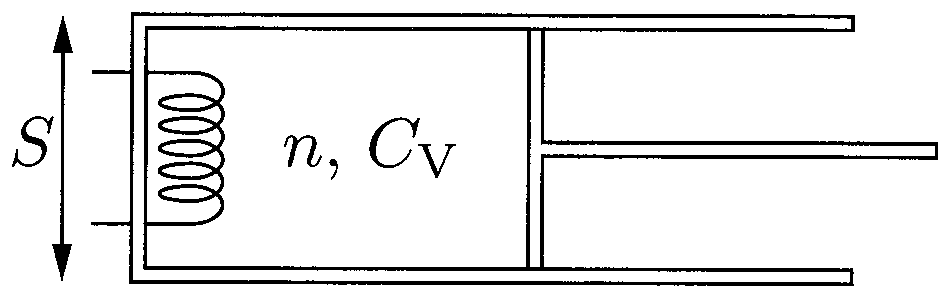
\includegraphics[keepaspectratio,width=58mm]{fig/ch17_p43_cyl.png}
\end{zuright}
\hspace{1zw}初め，シリンダーの底からピストンまでの距離は$l_0\U{m}$であり，また気体の温度は$T_0\U{K}$であった．シリンダー内にはヒーターが取り付けられており，気体に対して熱を与えることができる．シリンダーおよびピストンは断熱材でできており，ヒーターによって与えた熱が大気に拡散することはないものとする．気体定数を$R\U{J/mol\cdot K}$として以下の設問に答えよ．
\begin{komon}
\ko{1} 初めの状態におけるシリンダー内の気体の圧力$p_0\U{Pa}$を求めよ．
\end{komon}
\hspace{1zw}ここで，気体が温度$T_0\U{K}$を保つようにピストンを操作しながら内部の気体をヒーターでゆっくりと加熱したところ，ピストンはゆっくりと移動し，シリンダーの底からピストンまでの距離が$l_1\U{m}$となったところで加熱をやめた．
\begin{komon}
\ko{2} 終状態における気体の圧力$p_1\U{Pa}$を求めよ．
\ko{3} この変化において，気体が外界にした仕事$w\U{J}$を求めよ．
\ko{4} ヒーターによって加えた熱量$Q\U{J}$を求めよ．
\end{komon}

\Mon[\Sitei]{断熱変化}

\begin{zuright}{58mm}
\hspace{1zw}右図のように断面積$S\U{m^2}$のシリンダーの中に，ピストンで定積モル比熱が$C_V\U{J/mol\cdot K}$の理想気体を$n\U{mol}$だけ封入した．ピストンは軽くて自由に動くことができ，棒が取り付けられてある．
\zusep
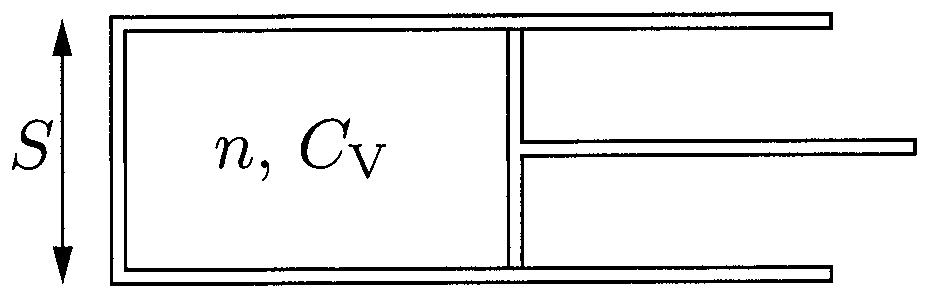
\includegraphics[keepaspectratio,width=58mm]{fig/ch17_p44_cyl.png}
\end{zuright}
\hspace{1zw}シリンダーおよびピストンは断熱材でできており，外界と熱のやり取りはない．棒を手で持って動かし，シリンダーの底からピストンまでの距離が$l_0\U{m}$となる位置に持ってきたところ気体の温度は$T_0\U{K}$となった．気体定数を$R\U{J/mol\cdot K}$として以下の設問に答えよ．
\begin{komon}
\ko{1} この状態におけるシリンダー内の圧力$p_0\U{Pa}$を求めよ．
\end{komon}
\hspace{1zw}ここでピストンを手でゆっくりと引き，シリンダーの底からピストンまでの距離が$l_1\U{m}$になるまで気体を膨張させた．
\begin{komon}
\ko{2} ポアソンの法則を用いて，終状態における気体の圧力$p_1\U{Pa}$および温度$T_1\U{K}$を求めよ．
% 誤植訂正（2026-09-02）：原本は「温度 T_1[K] 求めよ」で助詞「を」が欠けていた．
\ko{3} この状態変化を$p-V$図で表せ．
\ko{4} この変化において，気体が外界にした仕事$w\U{J}$を求めよ．
\end{komon}

\Mon{断熱自由膨張}

\begin{zuright}{56mm}
\hspace{1zw}右図のように，体積$V_\mathrm{A}\U{m^3}$, $V_\mathrm{B}\U{m^3}$の断熱容器A，Bをコックのついた細い管でつないである．はじめコックは閉じられており，Aだけに定積モル比熱$C_V\U{J/mol\cdot K}$の理想気体が圧力$p_0\U{Pa}$，温度$T_0\U{K}$となって入っている．コックを開いたところ気体はBへと拡散していき，十分時間が経つと全体が一様となった．このときA，B内の気体の圧力および温度を求めよ．ただし，気体定数を$R\U{J/mol\cdot K}$とする．
\zusep
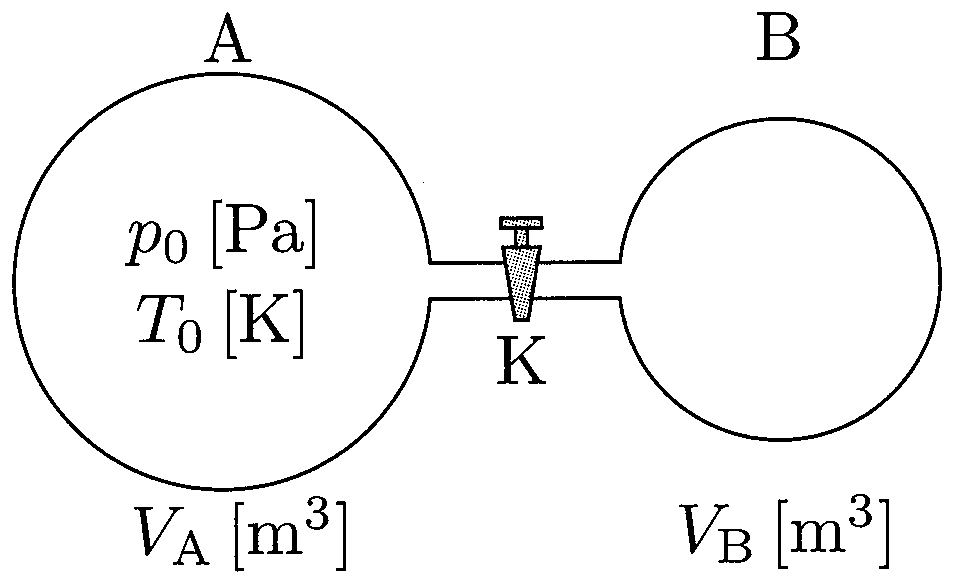
\includegraphics[keepaspectratio,width=56mm]{fig/ch17_p44_ab.png}
\end{zuright}

\Mon[\Sitei]{断熱膨張・断熱自由膨張}

\begin{zuright}{56mm}
\hspace{1zw}右図のようにバルブつきの隔壁で仕切られたシリンダーがある．隔壁の左側の体積は$V_0\U{m^3}$であり，ここに定積モル比熱$C_V\U{J/mol\cdot K}$の理想気体が圧力$p_0\U{Pa}$，温度$T_0\U{K}$となって封入されている．
\zusep
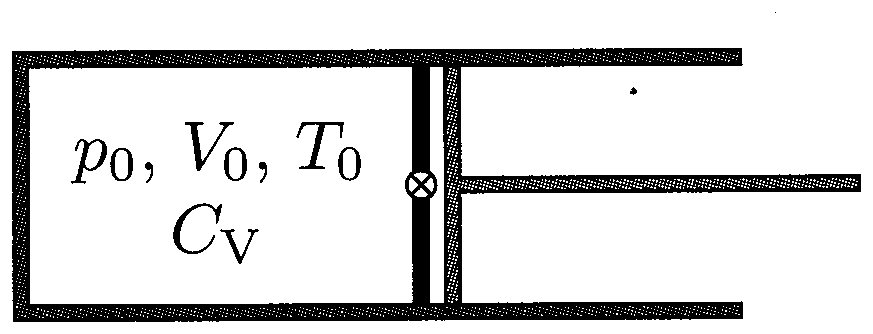
\includegraphics[keepaspectratio,width=56mm]{fig/ch17_p44_valve.png}
\end{zuright}
\hspace{1zw}隔壁の右側は取っ手付きのピストンが取り付けられている．初めバルブは閉じており，右側の空間には気体は封入されておらず，ピストンは隔壁に接触して体積が0になっている．シリンダー，ピストン，隔壁，バルブなどはすべて断熱材で出来ており，外界との熱のやり取りはない．

\hspace{1zw}この状態から以下の二つの方法によって左側に封入されている気体を右側に拡散させる．このとき，終状態における気体の圧力および温度をそれぞれ求めよ．気体定数を$R\U{J/mol\cdot K}$とする．
\begin{komon}
\ko{1} バルブを閉じたまま取っ手を引いて右側に体積$V_0\U{m^3}$の真空を作ったのち，バルブを全開にして気体を右側へ拡散させる．
\ko{2} バルブを全開にしてから取っ手をゆっくりと引き，右側の空間の体積を少しずつ増加させて体積$V_0\U{m^3}$にする．
\end{komon}

\filbreak
\Rank{C問題}

\Mon{気体の一般的な状態変化}

\begin{zuright}{62mm}
\hspace{1zw}図のように断面積$S\U{m^2}$のシリンダーに定積モル比熱が$C_V\U{J/mol\cdot K}$の理想気体を封入し，ピストンに図のように弾性定数が$k\U{N/m}$のバネを取り付けた．バネが自然長のとき，ちょうど大気圧$P_0\U{Pa}$とシリンダー内の気体の圧力とがつり合い，このときの気体の温度は$T_0\U{K}$，気柱の長さは$l_0\U{m}$であった．
\zusep
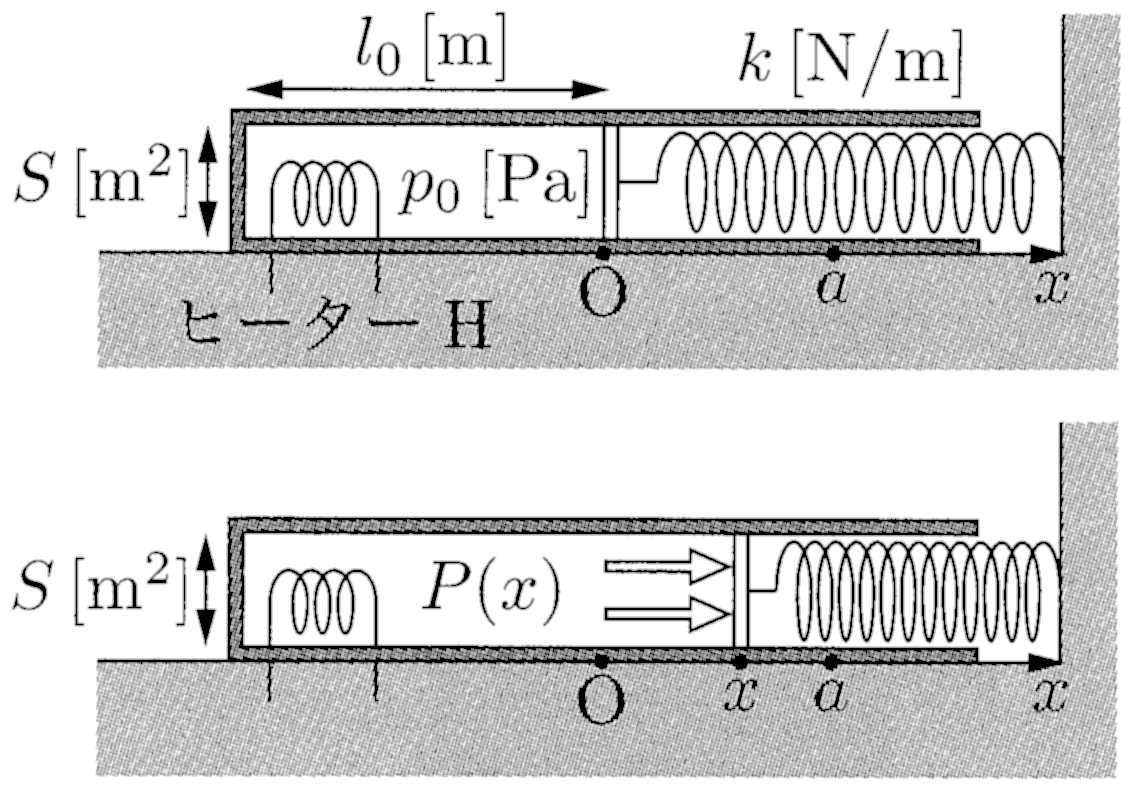
\includegraphics[keepaspectratio,width=62mm]{fig/ch17_p45_spring.png}
\end{zuright}
\hspace{1zw}シリンダー内のヒーターHから少しずつ気体を加熱していったところ，気体はゆっくりと膨張し，ピストンはゆっくりと距離$a\U{m}$だけ進んだ．シリンダー，容器などはすべて断熱材で出来ており，バネなどの熱容量は無視してよい．気体定数を$R\U{J/mol\cdot K}$として以下の設問に答えよ．
\begin{komon}
\ko{1} 終状態における気体の圧力$P_1\U{Pa}$および温度$T_1\U{K}$を求めよ．
\ko{2} この状態変化で気体がする仕事$w\U{J}$を求めよ．
\ko{3} この状態変化で気体に与えた熱量$Q\U{J}$を求めよ．
\end{komon}

\newpage

%%%%%%%%%%%%%%%%%%%%  解答（旧 prob_p132.png 〜 prob_p136_1.png）  %%%%%%%%%%%%%%%%%%%%
\KaiTitle{第17回　気体の状態変化\MARU{2}}
\setlength{\columnseprule}{0.4pt}
\begin{multicols}{2}
\raggedcolumns

\Rank{A問題}
\MonN{24}{基本事項の確認}\par\nopagebreak
\begin{sisin}
比熱比の定義式$\gamma=\dfrac{C_P}{C_V}$とマイヤーの関係式$C_P=C_V+R$を利用する．比熱比の分母・分子がどちらにくるかは，\underline{比熱比は}\hskip0pt\underline{必ず$1$}\hskip0pt\underline{より大}\hskip0pt\underline{きい}と覚えておけば間違いがない．
\end{sisin}
\KaiHead
マイヤーの関係式$C_P=C_V+R$を用いると，
\[\gamma=\frac{C_P}{C_V}=1+\frac{R}{C_V}\]
であるから，
\[\text{単原子分子理想気体：}\gamma=1+\frac{R}{\frac{3}{2}R}=\frac{5}{3}\]
\[\text{二原子分子理想気体：}\gamma=1+\frac{R}{\frac{5}{2}R}=\frac{7}{5}\Ans\]

\Rank{B問題}
\MonN{25}{状態変化に伴う各物理量の変化}\par\nopagebreak
\begin{sisin}
各状態変化で，熱量，仕事，内部エネルギーのどれが$0$になるのか（もしくは特殊な値・式となるのか）を覚えておき，残りの量については，$-W=\displaystyle\int_{V_{\mathrm{initial}}}^{V_{\mathrm{final}}}P(V)dV$, $\Delta U=nC_V\Delta T$, $\Delta U=Q+W$の各式から正負を判定する．

状態変化前後の状態方程式の両辺を差し引くと，
\[\begin{array}{r@{\;}l}
       & P_1V_1=nRT_1\\
 -)\;\;& P_0V_0=nRT_0\\ \hline
       & P_1V_1-P_0V_0=nR(T_1-T_0)
\end{array}\]
となる．ここで$PV$の項の変化$P_1V_1-P_0V_0$を$\Delta(PV)$と書くと，
\[\Delta(PV)=nR\cdot\Delta T\]
がすべての状態変化に対して成立する．温度変化についてはこれを利用して考えると便利である．
\end{sisin}
\KaiHead
状態変化前を$(P_0,V_0,T_0)$，変化後を$(P_1,V_1,T_1)$とする．$W$は外部が気体に対してした仕事であるから，気体が外部に対してした仕事は$(-W)$で表され，$-W=\displaystyle\int_{V_{\mathrm{initial}}}^{V_{\mathrm{final}}}P(V)dV$が成り立つ．内部エネルギーは絶対温度にのみ依存し$\Delta U=nC_V\Delta T$と表せる．また，熱力学の第一法則より$\Delta U=Q+W$，変化前後の状態方程式を辺々引いて，$P_1V_1-P_0V_0=nR(T_1-T_0)$が成り立つ．体積変化$\Delta V$を$\Delta V=V_1-V_0$とする．
\begin{komon}
\ko{1} 定圧であるから，$-W=P_0\cdot\Delta V$と表せる．\par
       \hspace*{1zw}圧縮しているので$\Delta V<0$であるから$W>0$，また$P_0\cdot\Delta V<0$であるから温度変化は$\Delta T<0$である．よって$\Delta U<0$となり，$Q=\Delta U+(-W)<0$である．
       \[\text{\MARU{1}負，\MARU{2}正，\MARU{3}負，\MARU{4}下降する}\Ans\]
\ko{2} 定積であるから$\Delta V=0$であり，$W=0$である．\par
       \hspace*{1zw}減圧していくので，$P_1V_0-P_0V_0<0$であるから温度変化は$\Delta T<0$である．よって$\Delta U<0$となり，$Q=\Delta U+(-W)<0$である．以上より，
       \[\text{\MARU{1}負，\MARU{2}$0$，\MARU{3}負，\MARU{4}下降する}\Ans\]
\ko{3} 定温であるから温度が一定であり，$\Delta U=0$である．\par
       \hspace*{1zw}加圧しているので$P_1>P_0$であり，状態方程式$P_1V_1=nRT_0$および$P_0V_0=nRT_0$より$V_1<V_0$, すなわち体積は減少している．よって$W>0$であり，$Q=\Delta U+(-W)<0$である．以上より，
       \[\text{\MARU{1}負，\MARU{2}正，\MARU{3}$0$，\MARU{4}一定である}\Ans\]
       \begin{chuu}
       気体が外部にした仕事$(-W)$の正負は$P-V$図から考えれば明らかである．定温曲線は次図のように双曲線となるのだから，加圧すれば体積は減少する．よって，$-W<0$となるのはこの図より明らか．
       % 誤植訂正（2026-09-02）：原本は「よって，W<0 となるのは…」．
       %   直前で「気体が外部にした仕事 (-W) の正負は」と述べており，加圧＝圧縮
       %   では (-W)<0（したがって W>0）．本解の(3)も「よって W>0 であり」と
       %   しているので，(-W)<0 に改めた．
       \begin{center}
       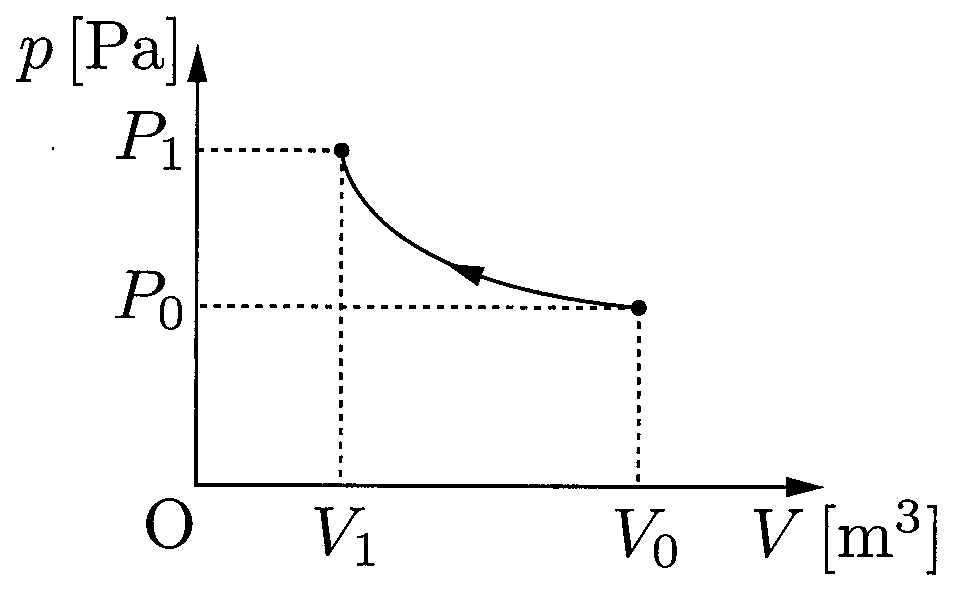
\includegraphics[keepaspectratio,width=54mm]{fig/ch17_a25_pv.png}
       \end{center}
       \end{chuu}
\ko{4} 断熱変化であるから，$Q=0$である．\par
       \hspace*{1zw}圧縮しているので$\Delta V<0$であるから$W>0$，また$\Delta U=Q+W$より$\Delta U>0$であるから温度変化は$\Delta T>0$である．以上より，
       \[\text{\MARU{1}$0$，\MARU{2}正，\MARU{3}正，\MARU{4}上昇する}\Ans\]
       \begin{chuu}
       (1)〜(4)の各状態変化ごとに本質的に覚えておくべきことは最初の一行のみである．あとは指針で述べた関係式から他の物理量の変化が分かる．
       \end{chuu}
\end{komon}

\MonN{26}{定温変化}\par\nopagebreak
\begin{sisin}
本問のように，変化途中で気体の圧力が変化する場合には$w=P\cdot\Delta V$としてはいけない．体積が$V\U{m^3}$のときの圧力$P(V)\U{Pa}$を求め，これを積分することで求める．
\end{sisin}
\KaiHead
\begin{komon}
\ko{1} 最初の状態について状態方程式を立てると，
       \[p_0\cdot Sl_0=nRT_0\]
       であるから，
       \[p_0=\frac{nRT_0}{Sl_0}\U{Pa}\Ans\]
\ko{2} 終状態における状態方程式は，
       \[p_1\cdot Sl_1=nRT_0\]
       であるから，
       \[p_1=\frac{nRT_0}{Sl_1}\U{Pa}\Ans\]
\ko{3} 気体の体積が$V\U{m^3}$のときの気体の圧力を$p(V)\U{Pa}$とし，このときの気体の状態方程式を立てると，
       \[p(V)\cdot V=nRT_0\]
       これより，
       \[p(V)=\frac{nRT_0}{V}\]
       よって，体積が$V=Sl_0\rightarrow Sl_1\U{m^3}$に変化するまでに気体が外部にした仕事$w$は，$nRT_0$が定数であることに注意して
       \[\begin{aligned}
         w&=\int_{Sl_0}^{Sl_1}p(V)dV=\int_{Sl_0}^{Sl_1}\frac{nRT_0}{V}dV\\
          &=nRT_0\int_{Sl_0}^{Sl_1}\frac{1}{V}dV\\
          &=nRT_0\Bigl[\log_e|V|\Bigr]_{Sl_0}^{Sl_1}\\
          &=nRT_0\log_e\frac{l_1}{l_0}\U{J}\Ans
       \end{aligned}\]
\ko{4} この状態変化にて気体の温度は$T_0$一定であるから，気体の内部エネルギー変化$\Delta U\U{J}$は
       \[\Delta U=nC_V\Delta T=0\]
       である．熱力学第一法則より$Q$, $\Delta U$, $w$の間には，
       \[\Delta U=Q+(-w)\]
       の関係が成り立つ．以上より気体に加えた熱量は
       \[Q=nRT_0\log_e\frac{l_1}{l_0}\U{J}\Ans\]
\end{komon}

\MonN{27}{断熱変化}\par\nopagebreak
\begin{sisin}
ピストンはゆっくりと移動するので，この状態変化は準静的過程である．理想気体の均一系準静的断熱変化では，ポアソンの式
\[PV^\gamma=（一定）,\;TV^{\gamma-1}=（一定）\]
が成立する．どちらの式を利用した方がよいかは問題文に与えられている文字で考えよ．本問では$p$, $T$の両方が問われているのでどちらを利用してもよい．前者の$pV^\gamma=（一定）$で考えた場合を示す．

断熱曲線の勾配は等温曲線よりも急になる．

\underline{断熱変化の}\hskip0pt\underline{場合に限}\hskip0pt\underline{り，$w$を}\hskip0pt\underline{熱力学第}\hskip0pt\underline{一法則か}\hskip0pt\underline{ら求める}\hskip0pt\underline{ことがで}\hskip0pt\underline{きる}．断熱変化の場合は$Q=0$であるから，$\Delta U$から$w$を求めることができるのである．もちろん$w=\displaystyle\int_{V_{\mathrm{initial}}}^{V_{\mathrm{final}}}P(V)dV$から求めることも可能である．
\end{sisin}
\KaiHead
気体の比熱比$\gamma$は，マイヤーの関係式を用いて，
\[\gamma=\frac{C_P}{C_V}=\frac{C_V+R}{C_V}=1+\frac{R}{C_V}\]
で与えられる．
\begin{komon}
\ko{1} 初めの状態について状態方程式を立てると，
       \[p_0Sl_0=nRT_0\]
       これを解いて，
       \[p_0=\frac{nRT_0}{Sl_0}\U{Pa}\Ans\]
\ko{2} 気体は外界と熱のやり取りをしておらず，断熱変化であるので，初状態と終状態に対してポアソンの式より，
       \[p_0(Sl_0)^\gamma=p_1(Sl_1)^\gamma\]
       が成り立つ．これを解いて，
       \[p_1=\frac{nRT_0}{Sl_0}\left(\frac{l_0}{l_1}\right)^{1+\frac{R}{C_V}}\U{Pa}\Ans\]
       また，終状態の状態方程式は，
       \[p_1Sl_1=nRT_1\]
       であるから，これを解いて
       \[T_1=T_0\left(\frac{l_0}{l_1}\right)^{\frac{R}{C_V}}\U{K}\Ans\]
       \begin{bekkai}
       もう一つのポアソンの式$TV^{\gamma-1}=$一定を利用してもよい．この場合は，
       \[T_0(Sl_0)^{\gamma-1}=T_1(Sl_1)^{\gamma-1}\]
       より，$T_1=T_0\left(\dfrac{l_0}{l_1}\right)^{\frac{R}{C_V}}\U{K}$を導くことができる．また，この$T_1$を元に終状態の状態方程式$p_1Sl_1=nRT_1$を立てて圧力$p_1$を求めることが可能である．

       ポアソンの式は多少面倒な式であるから，まず$pV^\gamma=$一定もしくは$TV^{\gamma-1}=$一定を用いて変化後の$p$, $T$のいずれか一方を求め，もう片方については状態方程式から求めればよい．両方をポアソンの式から求めるのは面倒なだけである．
       \end{bekkai}
\ko{3} 気体の体積が$V\U{m^3}$のときの気体の圧力を$p(V)\U{Pa}$とし，初状態とこの状態との間にポアソンの式より，
       \[p(V)V^\gamma=p_0(Sl_0)^\gamma\quad(=\text{一定})\]
       が成り立つ．よって，
       \[p(V)=p_0(Sl_0)^\gamma\frac{1}{V^\gamma}\]
       である．ここで$\gamma>1$に注意すると，これは右下がりの曲線を表すので，状態変化の$p-V$図は次図の通り．
       \begin{center}
       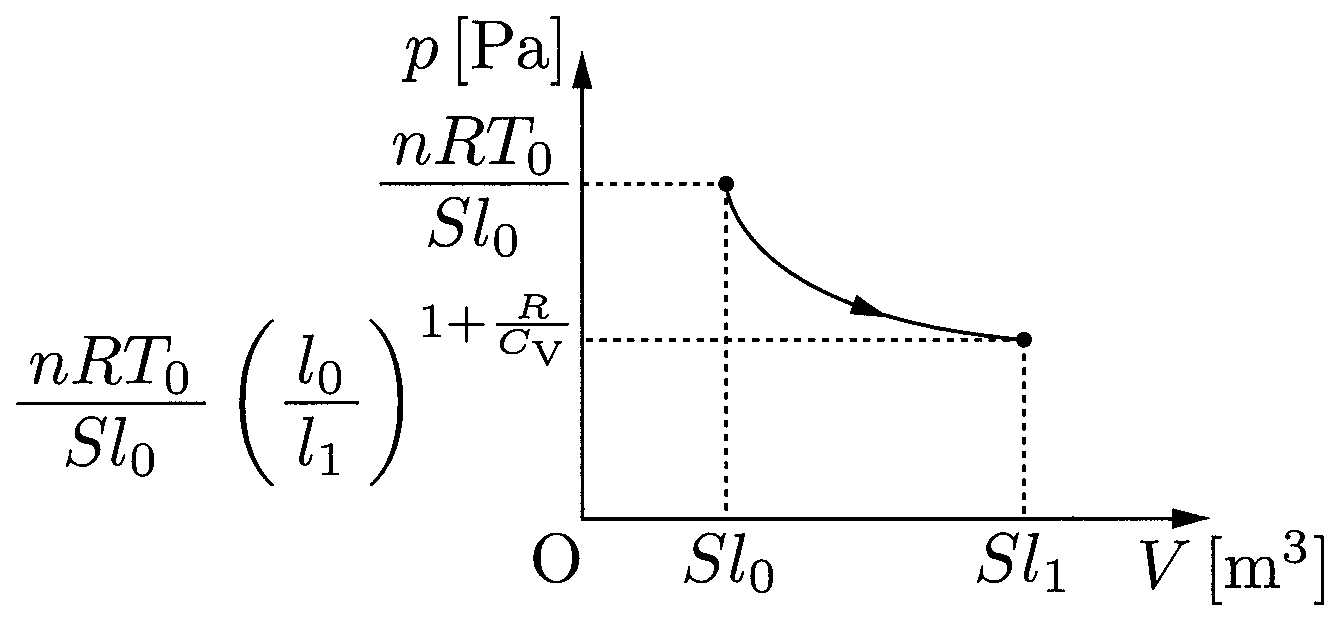
\includegraphics[keepaspectratio,width=64mm]{fig/ch17_a27_pv.png}
       \end{center}
       \hspace*{\fill}\Ans
\ko{4} この変化は断熱変化であるから，外部が気体に与える熱量$Q$は，
       \[Q=0\]
       また，この状態変化の内部エネルギーの増加量$\Delta U$は，
       \[\begin{aligned}
         \Delta U&=nC_V(T_1-T_0)\\
                 &=nC_VT_0\left\{\left(\frac{l_0}{l_1}\right)^{\frac{R}{C_V}}-1\right\}\U{J}
       \end{aligned}\]
       気体が外界に対してした仕事$w$は，熱力学第一法則を用いると，
       \[\Delta U=Q+(-w)\]
       の関係があるので，
       \[\begin{aligned}
         w&=-\Delta U\\
          &=nC_VT_0\left\{1-\left(\frac{l_0}{l_1}\right)^{\frac{R}{C_V}}\right\}\U{J}\Ans
       \end{aligned}\]
       \begin{bekkai}
       指針でも述べたように，まともに
       \[w=\int_{V_{\mathrm{initial}}}^{V_{\mathrm{final}}}P(V)dV\]
       を計算しても同一の答えが求められる．気体の体積が$V\U{m^3}$のときの気体の圧力$p(V)\U{Pa}$は，
       \[p(V)=p_0(Sl_0)^\gamma\frac{1}{V^\gamma}\]
       であるから，
       \[\begin{aligned}
         w&=\int_{Sl_0}^{Sl_1}p(V)dV\\
          &=p_0(Sl_0)^\gamma\int_{Sl_0}^{Sl_1}\frac{1}{V^\gamma}dV\\
          &=p_0(Sl_0)^\gamma\left[\frac{1}{-\gamma+1}V^{-\gamma+1}\right]_{Sl_0}^{Sl_1}\\
          &=p_0(Sl_0)^\gamma\left[-\frac{C_V}{R}\cdot\frac{1}{V^{\gamma-1}}\right]_{Sl_0}^{Sl_1}\\
          &=-\frac{C_V}{R}p_0(Sl_0)^{\gamma-1}(Sl_0)\\
          &\qquad\times\left\{\frac{1}{(Sl_1)^{\gamma-1}}-\frac{1}{(Sl_0)^{\gamma-1}}\right\}\\
          &=-\frac{C_V}{R}p_0(Sl_0)\left\{\left(\frac{l_0}{l_1}\right)^{\gamma-1}-1\right\}\\
          &=\frac{C_V}{R}\frac{nRT_0}{Sl_0}Sl_0\left\{1-\left(\frac{l_0}{l_1}\right)^{\frac{R}{C_V}}\right\}\\
          &=nC_VT_0\left\{1-\left(\frac{l_0}{l_1}\right)^{\frac{R}{C_V}}\right\}\U{J}
       \end{aligned}\]
       となり，全く同じ答えが導ける．しかし，この計算はなかなかに厄介である．断熱変化に限っては熱力学第一法則から$w$を求めることを覚えておくとよい．
       \end{bekkai}
\end{komon}

\MonN{28}{断熱自由膨張}\par\nopagebreak
\begin{sisin}
本問のような断熱自由膨張では，\underline{容器$\mathrm{A+B}$}\hskip0pt\underline{全体を一}\hskip0pt\underline{つの系と}\hskip0pt\underline{みなして}\hskip0pt\underline{熱力学第}\hskip0pt\underline{一法則を}\hskip0pt\underline{立てる}のがポイント．$\mathrm{A+B}$の全体積は$V_\mathrm{A}+V_\mathrm{B}\U{m^3}$のまま不変であるから，$\mathrm{A+B}$は容器外と仕事のやり取りをしない．また，断熱容器を使っているから熱のやり取りもない．以上に着目して熱力学第一法則を立てる．
\end{sisin}
\KaiHead
変化後の$\mathrm{A}$, $\mathrm{B}$内の気体の圧力を$p\U{Pa}$, 温度を$T\U{K}$とする．この変化において，$\mathrm{A+B}$を一つの系とみなすと，これは体積が不変であるから外界と仕事のやり取りをせず，また断熱容器を利用しているので外界と熱のやり取りもしない．よって，内部エネルギーの変化量を$\Delta U$とすると，熱力学第一法則より，
\[\Delta U=0+0\]
と立式できる．$\Delta U$は絶対温度に比例し，
\[\Delta U=nC_V\Delta T=0\]
と表せるので，これより$\Delta T=0$, すなわち気体の温度は変化しない．
\[T=T_0\U{K}\Ans\]
また状態変化前の$\mathrm{A}$内の気体のモル数を$n$とすると，状態方程式は，
\[p_0V_\mathrm{A}=nRT_0\]
また状態変化後は$\mathrm{A+B}$に一様に気体が広がっているので$\mathrm{A+B}$全体に対して状態方程式を立てることができ，
\[p(V_\mathrm{A}+V_\mathrm{B})=nRT_0\]
となる．以上2式を組み合わせて，
\[p=\frac{V_\mathrm{A}}{V_\mathrm{A}+V_\mathrm{B}}p_0\U{Pa}\Ans\]

\MonN{29}{断熱膨張・断熱自由膨張}\par\nopagebreak
\begin{sisin}
(1)も(2)もいずれも断熱変化であり，最終的には全体積$2V_0\U{m^3}$の空間に気体が広がることになるが，(1)の方法と(2)の方法は全く異なる．(1)は前問と全く同じで，真空中への拡散である．一方，(2)は，バルブを全開にしてからゆっくりと引いているのだから，バルブはないのと同じことである．よって，これは準静的な断熱膨張で，ポアソンの式を利用して考えればよい．
\end{sisin}
\KaiHead
気体のモル数を$n\U{mol}$とすると，最初の状態の状態方程式は
\[p_0V_0=nRT_0\]
である．
\begin{komon}
\ko{1} この方法では，次図のようにいったん右側に体積$V_0\U{m^3}$の真空を作り，左側から右側へ気体を拡散させていくので断熱自由膨張だとみなせる．
       \begin{center}
       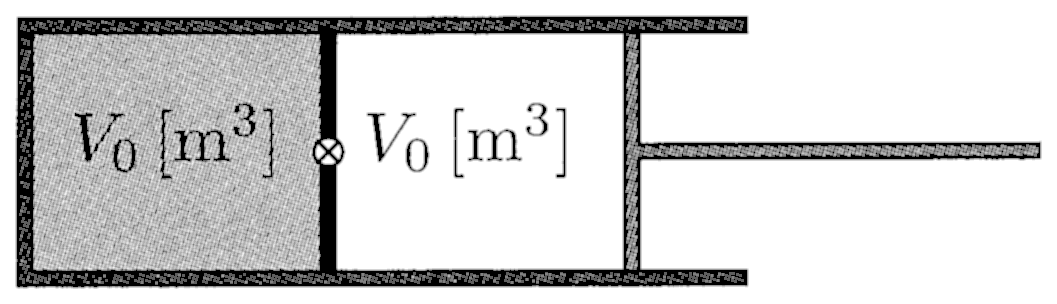
\includegraphics[keepaspectratio,width=62mm]{fig/ch17_a29_1.png}
       \end{center}
       よって，左側の空間と右側の空間を一つの系だとみなすと，この系は外界との仕事のやり取り，熱のやり取りがない．内部エネルギーの変化量を$\Delta U\U{J}$とすると，熱力学第一法則より$\Delta U=0+0$となる．内部エネルギーは絶対温度に比例するので，全体に拡がる前後で温度変化はなく，変化後の気体の温度を$T_1\U{K}$とおくと，
       \[T_1=T_0\U{K}\Ans\]
       また，このときの気体の圧力を$p_1\U{Pa}$とする．最終的には容器全体に気体が一様に拡がっているので，全体に対して状態方程式を立てることができ，
       \[p_1\cdot 2V_0=nRT_0\]
       \begin{center}
       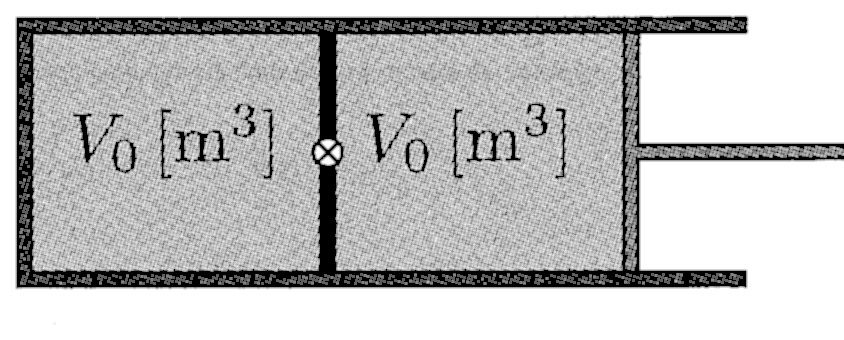
\includegraphics[keepaspectratio,width=54mm]{fig/ch17_a29_2.png}
       \end{center}
       これと最初の状態方程式とを組み合わせて解くと，
       \[p_1=\frac{1}{2}p_0\U{Pa}\Ans\]
\ko{2} バルブを全開にしてから取っ手をゆっくりと引く場合，バルブを通して気体は右側へと十分に拡散することができるので，例えば右側の体積が$V\U{m^3}$となったときには，気体は次の図のように左側と右側とにムラなく広がっている．
       \begin{center}
       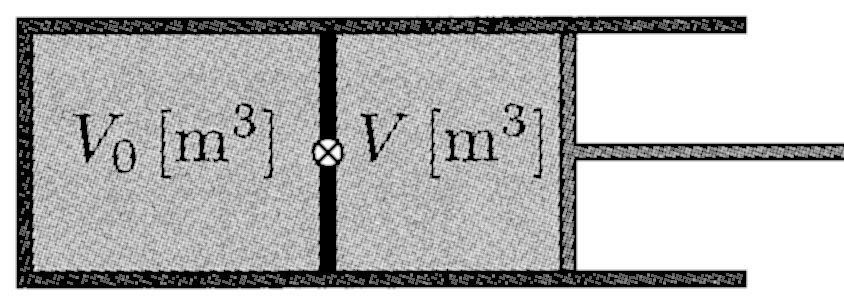
\includegraphics[keepaspectratio,width=54mm]{fig/ch17_a29_3.png}
       \end{center}
       すなわち，この状態変化ではバルブは存在しないのと全く同様にみなせるので，この状態変化は次図と全く同じものとみなせる．
       \begin{center}
       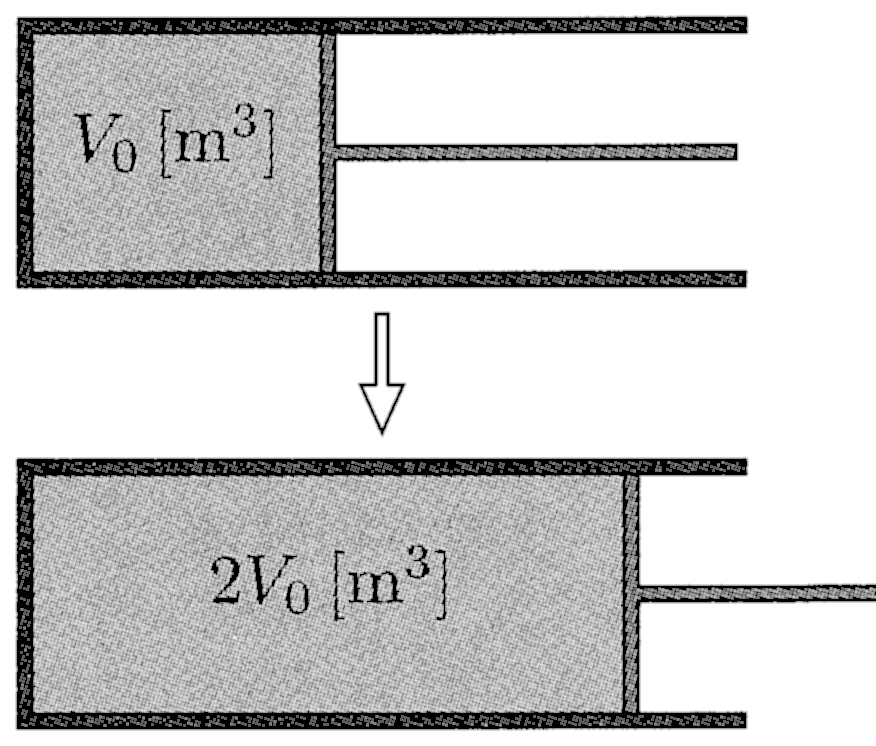
\includegraphics[keepaspectratio,width=52mm]{fig/ch17_a29_4.png}
       \end{center}
       よって，この断熱変化に対してはポアソンの式を適用することができる．この気体の比熱比$\gamma$は
       \[\gamma=\frac{C_P}{C_V}=\frac{C_V+R}{C_V}=1+\frac{R}{C_V}\]
       で与えられるので，終状態の圧力を$p_2\U{Pa}$とすると，ポアソンの式より，
       \[p_0V_0^\gamma=p_2(2V_0)^\gamma\]
       が成立する．これを解いて，
       \[p_2=\frac{1}{2^\gamma}p_0=\frac{1}{2^{1+R/C_V}}p_0\U{Pa}\Ans\]
       また，終状態での温度を$T_2\U{K}$とおくと，状態方程式を立てると，
       \[p_2\cdot 2V_0=nRT_2\]
       よって，
       \[T_2=\frac{1}{2^{R/C_V}}T_0\U{K}\Ans\]
       \begin{bsHosoku}{参考}
       二つの変化それぞれの正しい解法は上述した通りだが，ではなぜ(1)の場合にポアソンの式が利用できないのか？

       それは，(1)の状態変化では，変化途中（すなわち左から右へと気体が拡散している途中）において，気体全体を一つの均一系とみなすことができないからである．

       次の図にあるように，気体が左から右へ拡散していく途中では左の気体の方が気体の密度，圧力が高い．そのため，左，右のそれぞれについて状態方程式を立てることはできるが，左＋右をひとくくりにして状態方程式を立てることができない（圧力が共通ではないから）．
       \begin{center}
       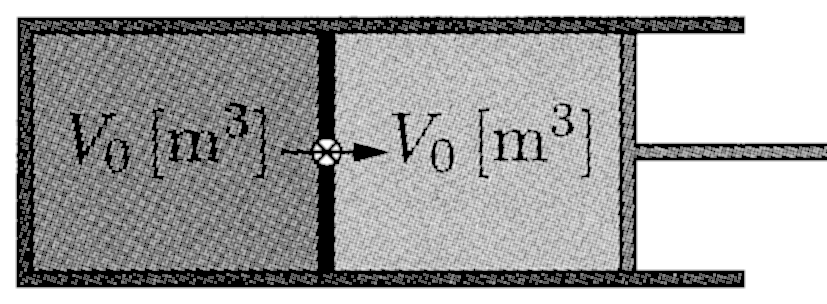
\includegraphics[keepaspectratio,width=54mm]{fig/ch17_a29_ref.png}
       \end{center}
       ポアソンの式の導出では気体全体に対しての状態方程式を利用しているので，(1)のような断熱自由膨張に対してはポアソンの式を利用することができないのである．
       \end{bsHosoku}
\end{komon}

\Rank{C問題}
\MonN{30}{気体の一般的な状態変化}\par\nopagebreak
\begin{sisin}
本問はバネがあるため，気体の状態変化は定積，定圧，定温，断熱のいずれにも当てはまらない．このような場合には，全ての状態変化に対して成立する次の基本的な流れに従って考えよ．
\begin{list}{}{\setlength{\leftmargin}{1.6zw}\setlength{\itemsep}{0.3mm}\setlength{\topsep}{0.6mm}\setlength{\parsep}{0pt}}
\item[\MARU{1}] $w=\displaystyle\int_{V_{\mathrm{start}}}^{V_{\mathrm{end}}}P(V)dV$の計算
\item[\MARU{2}] $\Delta U=nC_V\Delta T$の計算
\item[\MARU{3}] 熱力学第一法則$\Delta U=Q+(-w)$の立式
\end{list}
\end{sisin}
\KaiHead
問題の図にある，バネが距離$x\U{m}$だけ縮んだ途中状態における気体の圧力を$P(x)$とすると，ピストンに対して作用する力のつり合いより，
\[P(x)S=P_0S+kx\]
これより，
\[P(x)=P_0+\frac{kx}{S}\U{Pa}\]
また，このときの体積は
\[V(x)=S(l_0+x)\U{m^3}\]
封入されている気体のモル数を$n\U{mol}$とすると，最初の状態の状態方程式は
\[P_0\cdot Sl_0=nRT_0\]
である．
\begin{komon}
\ko{1} 終状態，すなわち$x=a\U{m}$のときは，
       \[P_1=P(a)=P_0+\frac{ka}{S}\U{Pa}\Ans\]
       であり，このときの気体の状態方程式は
       \[P_1\cdot S(l_0+a)=nRT_1\]
       これと最初の状態の状態方程式を組み合わせて解くと，
       \[T_1=\left(1+\frac{ka}{P_0S}\right)\left(1+\frac{a}{l_0}\right)T_0\U{K}\Ans\]
\ko{2} この状態変化で気体がする仕事は，積分を用いて
       \[w=\int_{Sl_0}^{S(l_0+a)}P(V)dV\]
       で求められる．この式の積分変数を$V$から$x$に変えると，
       \[\frac{dV}{dx}=S\;\Leftrightarrow\;dV=Sdx\]
       \[V=S(l_0+a)\;\Leftrightarrow\;x=a\]
       \[V=Sl_0\;\Leftrightarrow\;x=0\]
       であるから，
       \[\begin{aligned}
         w&=\int_0^a\left(P_0+\frac{kx}{S}\right)Sdx\\
          &=\int_0^a(P_0S+kx)dx\\
          &=P_0Sa+\frac{1}{2}ka^2\U{J}\Ans
       \end{aligned}\]
       \begin{chuu}
       圧力$P$を体積$V$で表してもよい．
       \[P(x)=P_0+\frac{kx}{S}\U{Pa}\]
       \[V(x)=S(l_0+x)\U{m^3}\]
       の2式から$x$を消すと，
       \[P(V)=P_0+\frac{k}{S}\left(\frac{V}{S}-l_0\right)\U{Pa}\]
       が得られる．これをもとに$p-V$図を描き，その面積から仕事を求めることができる．
       \end{chuu}
\ko{3} この状態変化での内部エネルギーの増加は
       \[\Delta U=nC_V(T_1-T_0)\]
       であり，熱力学第一法則$\Delta U=Q+(-w)$を利用すると，
       \[\begin{aligned}
         Q&=nC_VT_0\left(\frac{ka}{P_0S}+\frac{a}{l_0}+\frac{ka^2}{P_0Sl_0}\right)\\
          &\qquad\qquad\qquad+P_0Sa+\frac{1}{2}ka^2\U{J}\\
          &=\frac{C_V}{R}kal_0+\frac{2C_V+R}{2R}ka^2\\
          &\qquad\qquad\qquad+\frac{C_V+R}{R}P_0Sa\U{J}\Ans
       \end{aligned}\]
\end{komon}

\end{multicols}

\section{熱力学総合演習}

\subsection{熱機関}
いくつかの状態変化を組み合わせ，最初の状態に戻るような過程を{\bf 熱機関}，または{\bf 熱サイクル}と呼ぶ．
最初の状態に戻るので，トータルで温度変化はないことから内部エネルギーの変化量は0[J]である．
熱機関の過程には熱を吸収する吸熱過程と熱を放出する放熱過程がある．
吸熱過程における吸熱量の合計を$Q_{in}$[J]．放熱過程における放熱量を$Q_{out}$とすれば，熱力学第一法則より，熱機関1周で気体が外にする仕事の合計$W_{サイクル}$[J]は
\[W_{サイクル}=Q_{in}-Q_{out}\]
と表せる．

熱機関での1周のエネルギーの変化を，$Q_{in}$[J]の熱を与え，そのうち$W_{サイクル}$[J]分だけ仕事をし，あまりのエネルギー$Q_{out}$[J]を熱として捨てていると解釈できる．
このときの加えた熱量に対してどれだけの仕事をするかを{\bf 熱効率}と呼び，熱効率$e$は
\[\mbox{\boldmath $e=\dfrac{W_{サイクル}}{Q_{in}} =1-\dfrac{Q_{out}}{Q_{in}}$}\]
となる．

また，各過程での$P-V$図における符号付き面積を考えることで，仕事の合計$W_{サイクル}$[J]は熱機関の各過程で囲まれた部分の符号付き面積として表すことができる．
 \begin{figure}[h]
\begin{center}
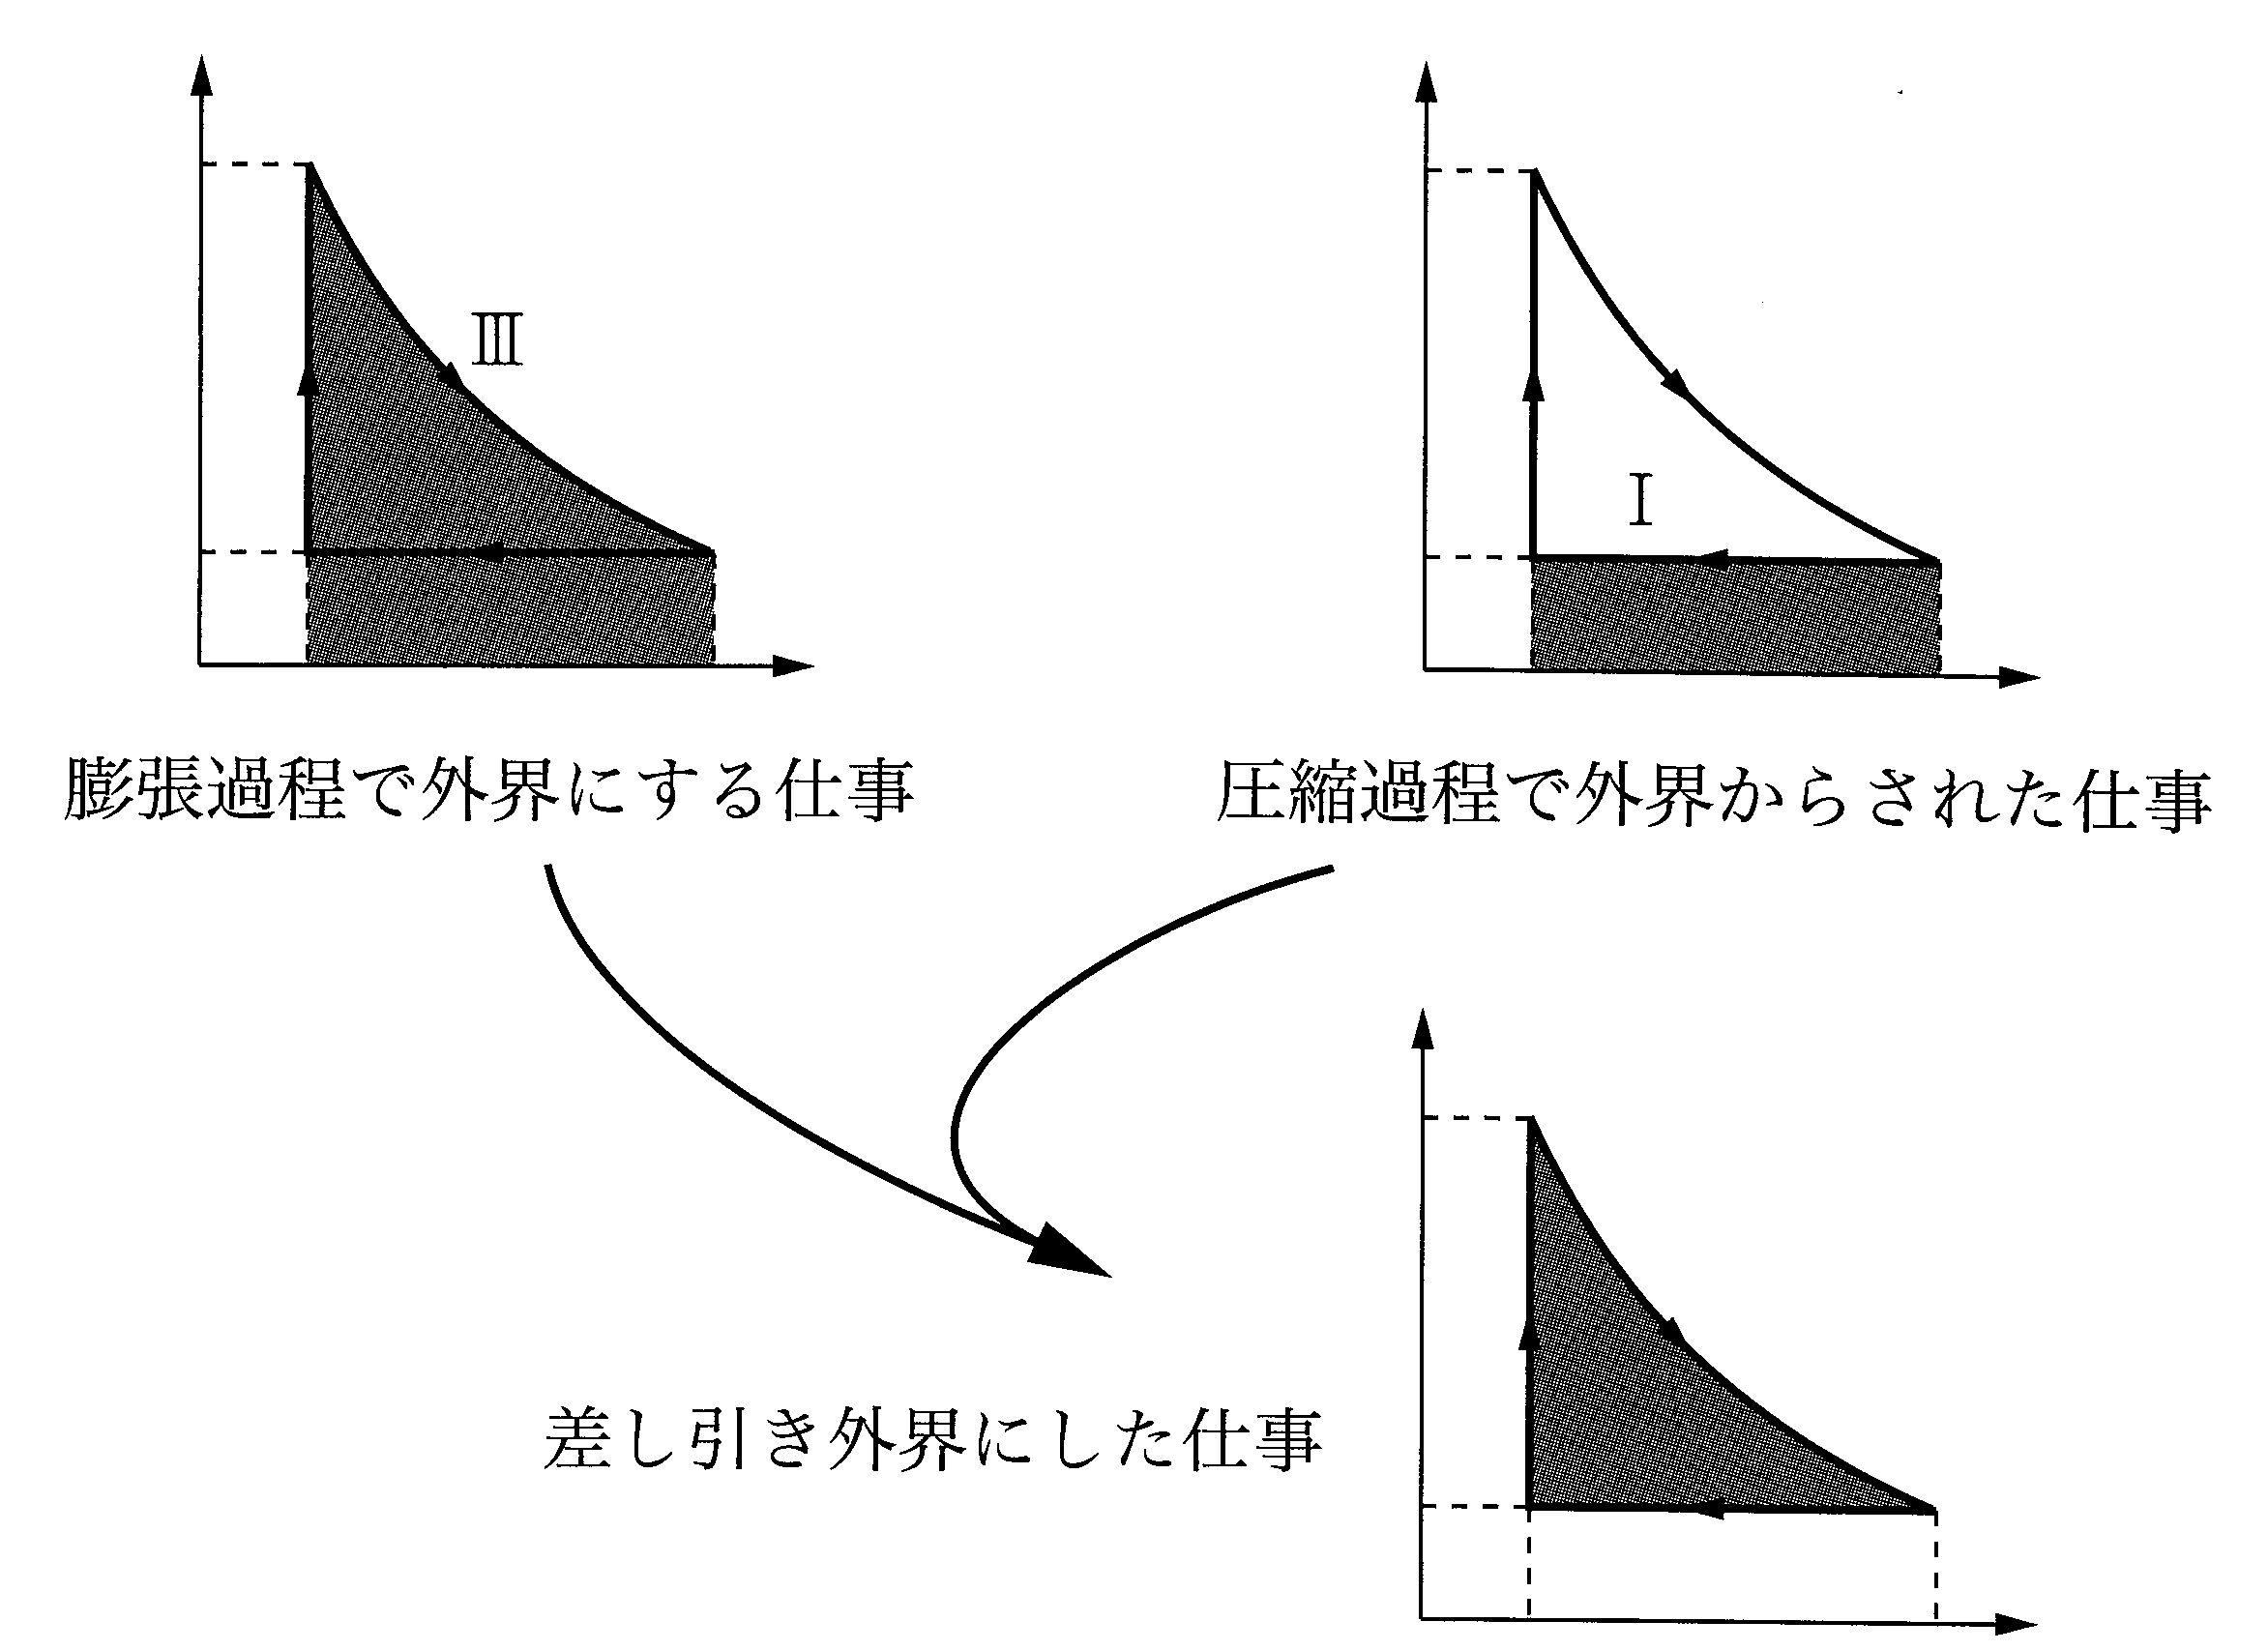
\includegraphics[width=100mm]{text_p84_fig1.png}
\end{center}
\end{figure}

このとき，時計回りに回る熱機関ならば$W_{サイクル}>0$となり面積と等しいが，反時計回りに回る場合は$W_{サイクル}<0$となり，面積に$-1$をかけた値となる．


\newpage

\begin{figure}[h]
\begin{center}
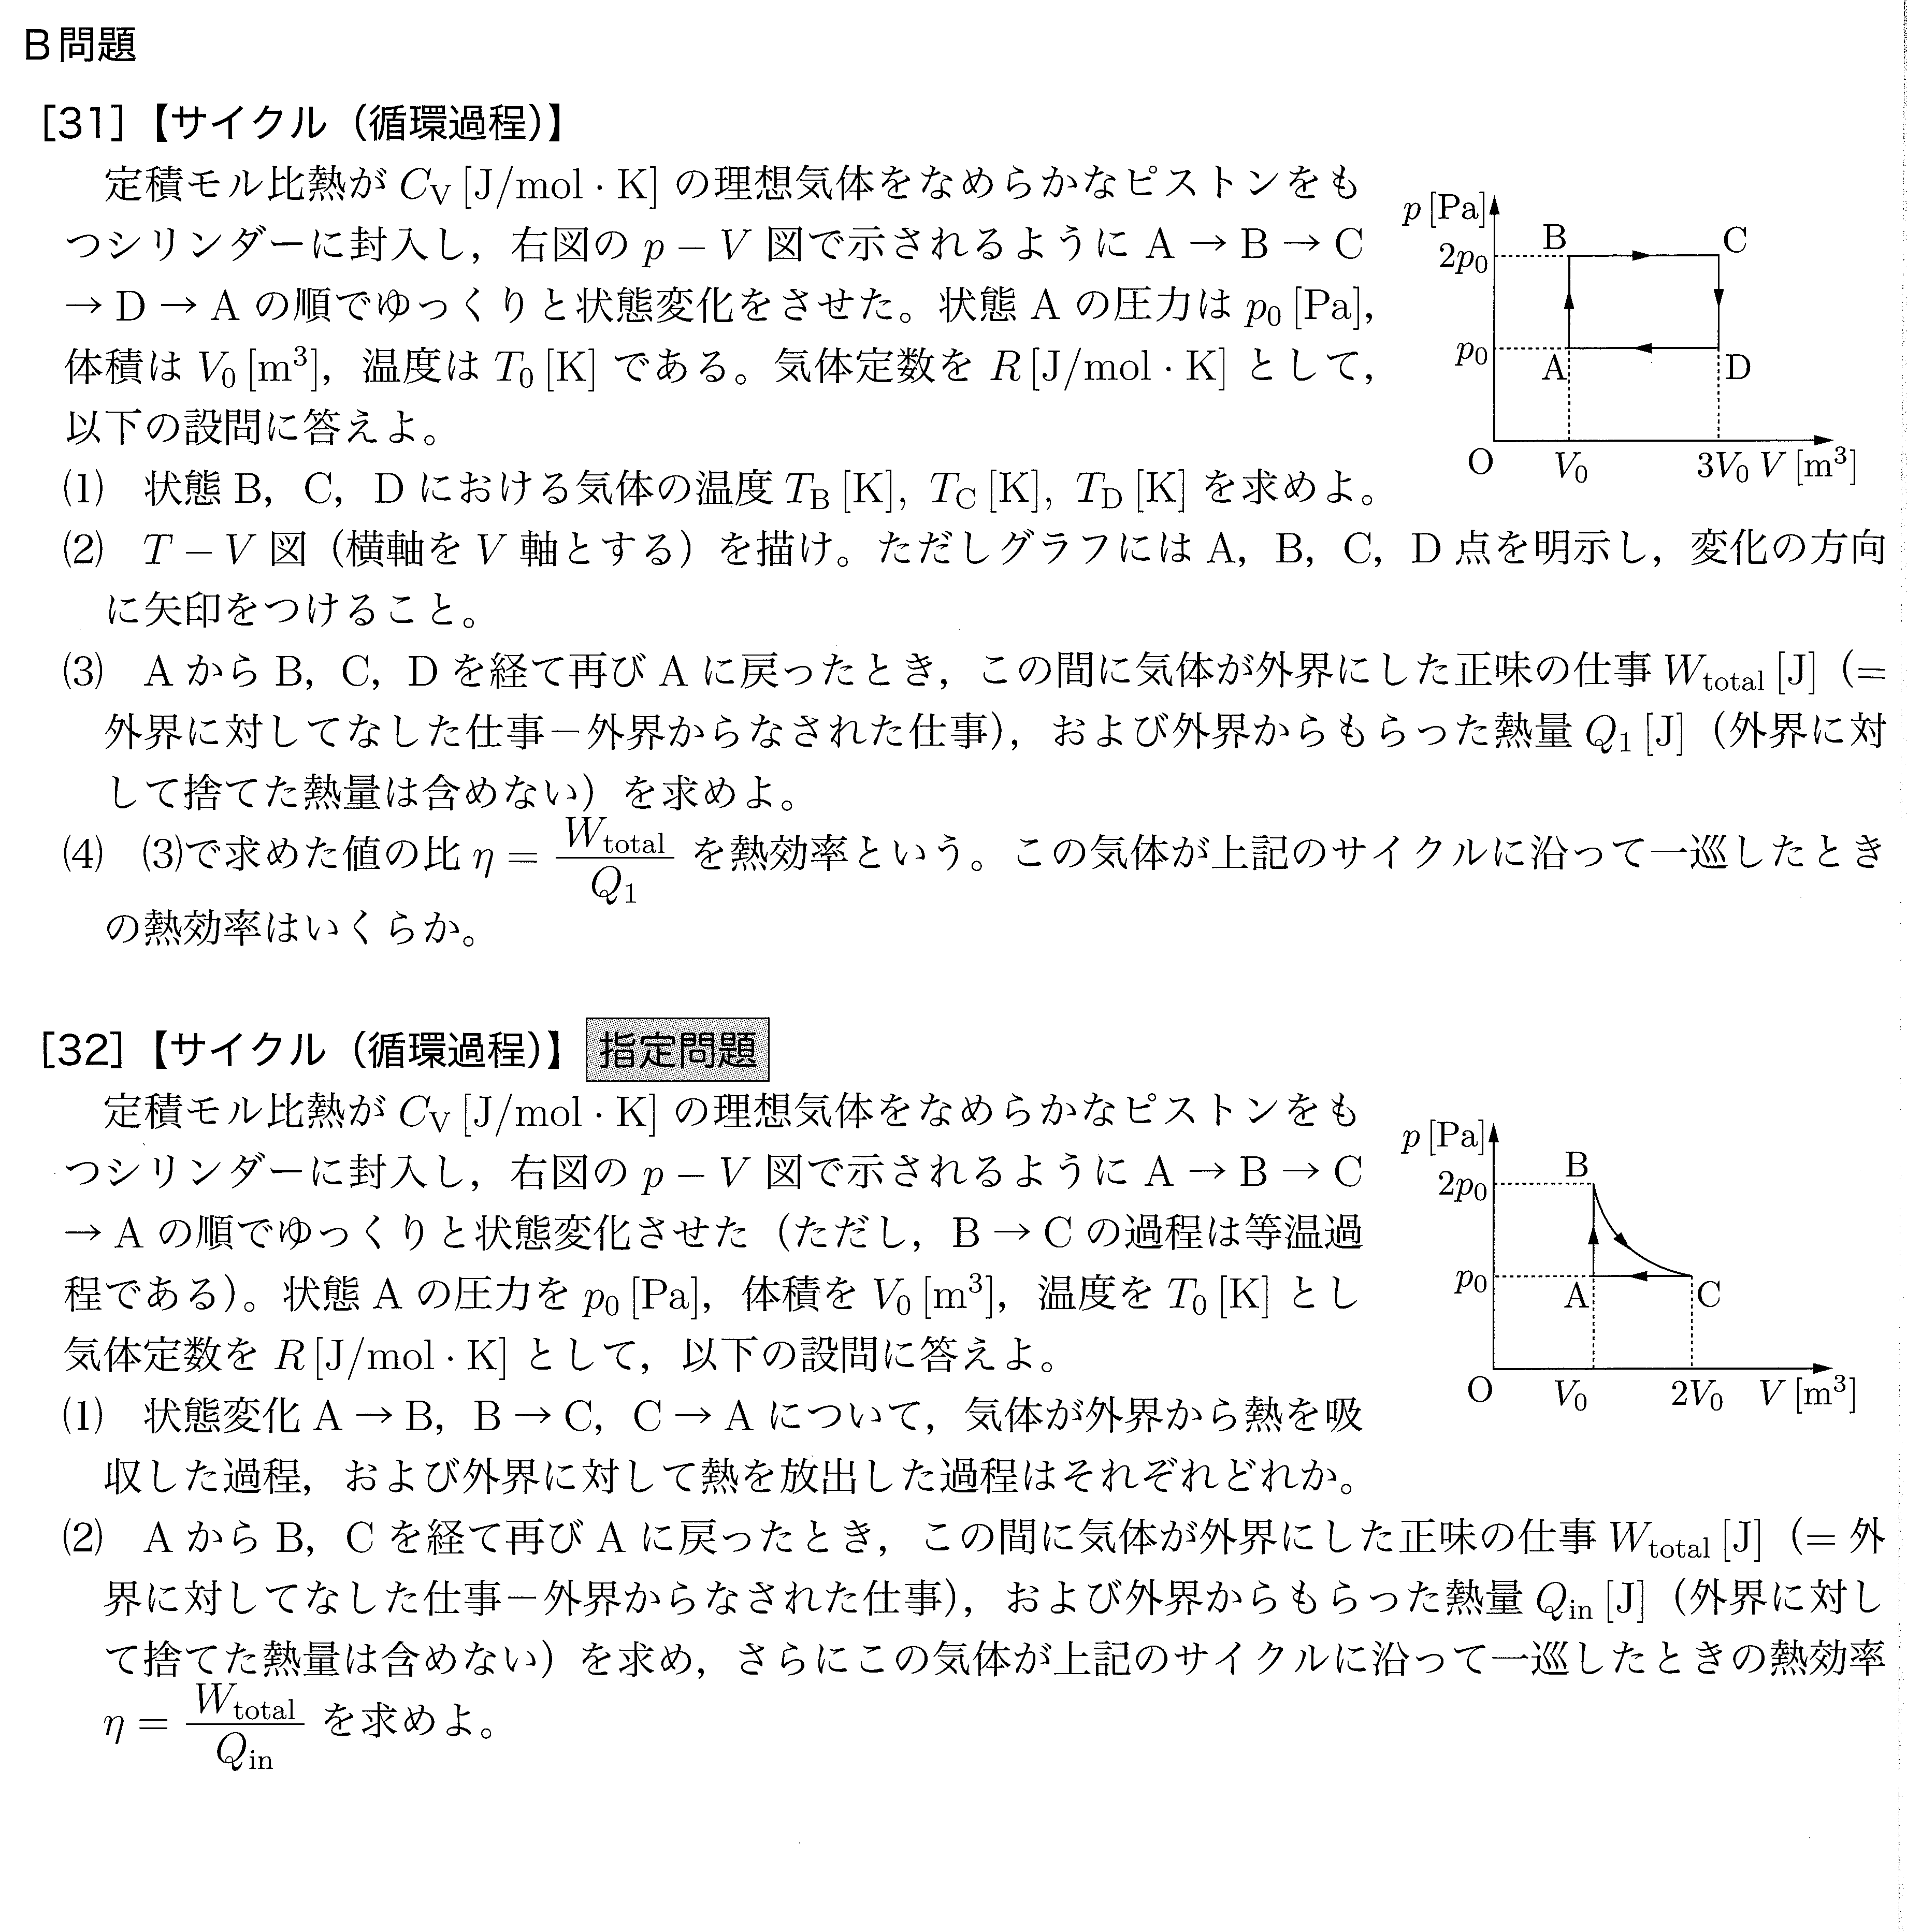
\includegraphics[width=170mm]{prob_p46.png}
\end{center}
\end{figure}

\newpage

\begin{figure}[h]
\begin{center}
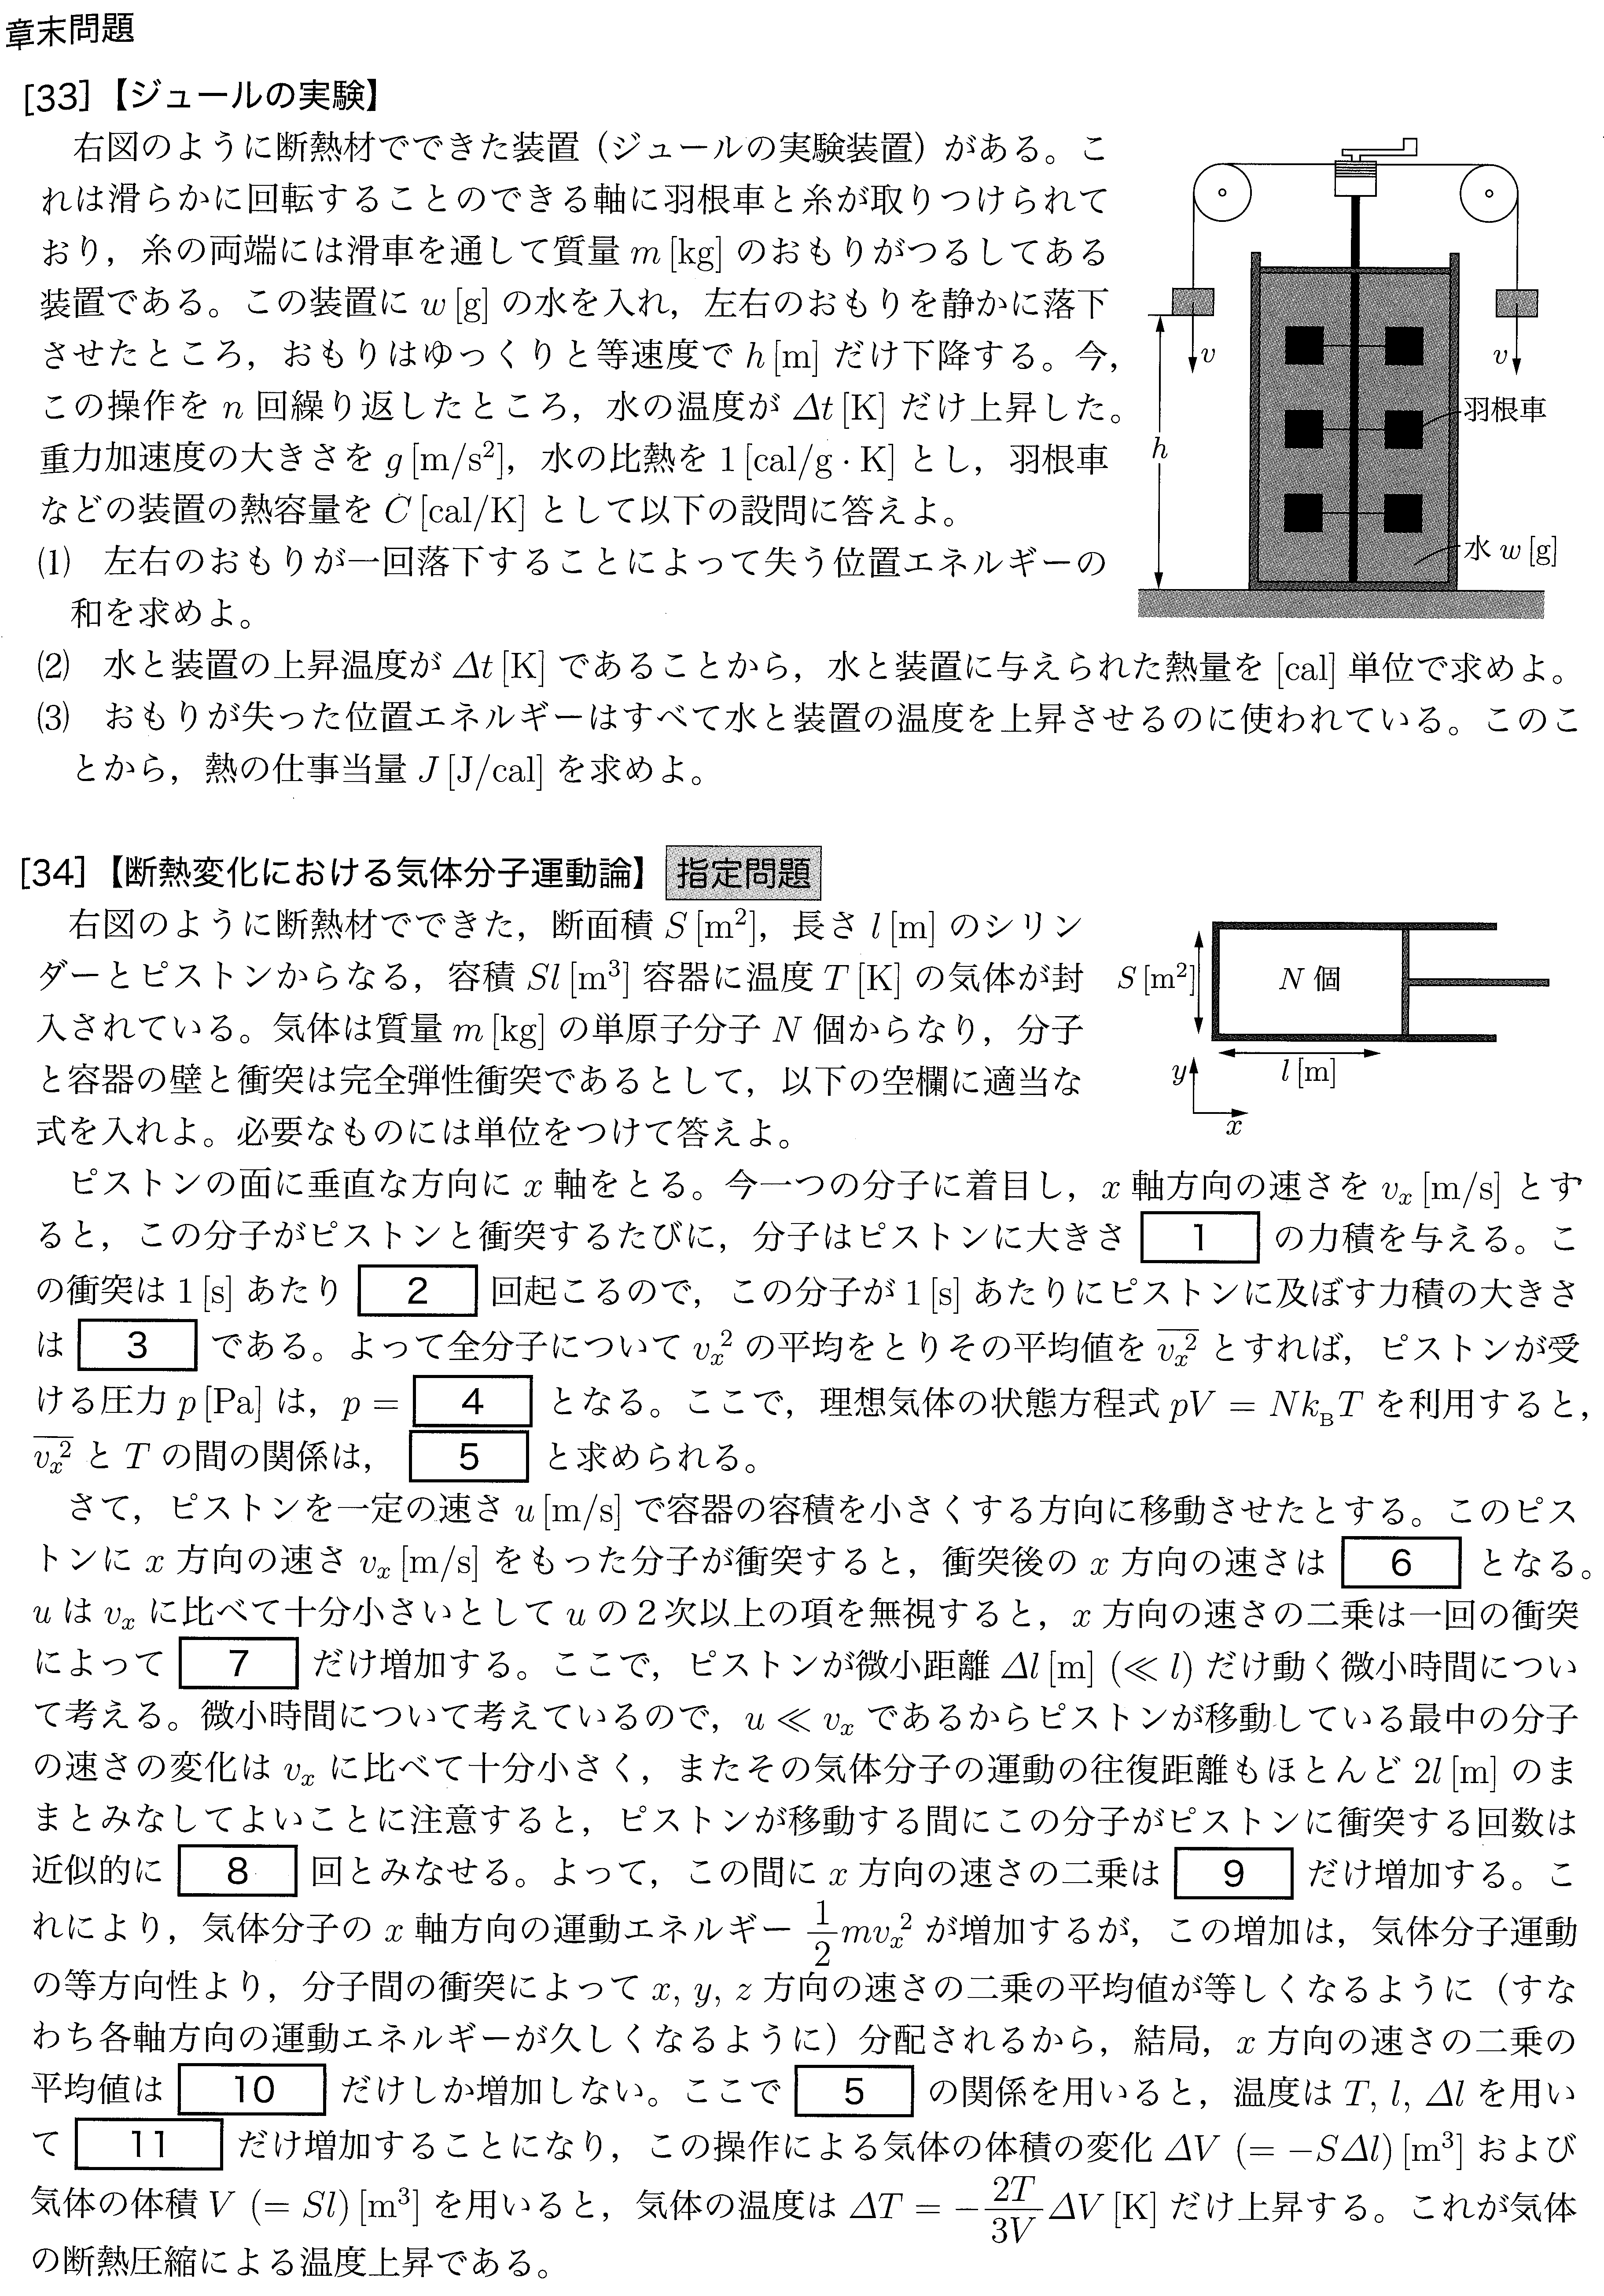
\includegraphics[width=170mm]{prob_p47.png}
\end{center}
\end{figure}

\newpage

\begin{figure}[h]
\begin{center}
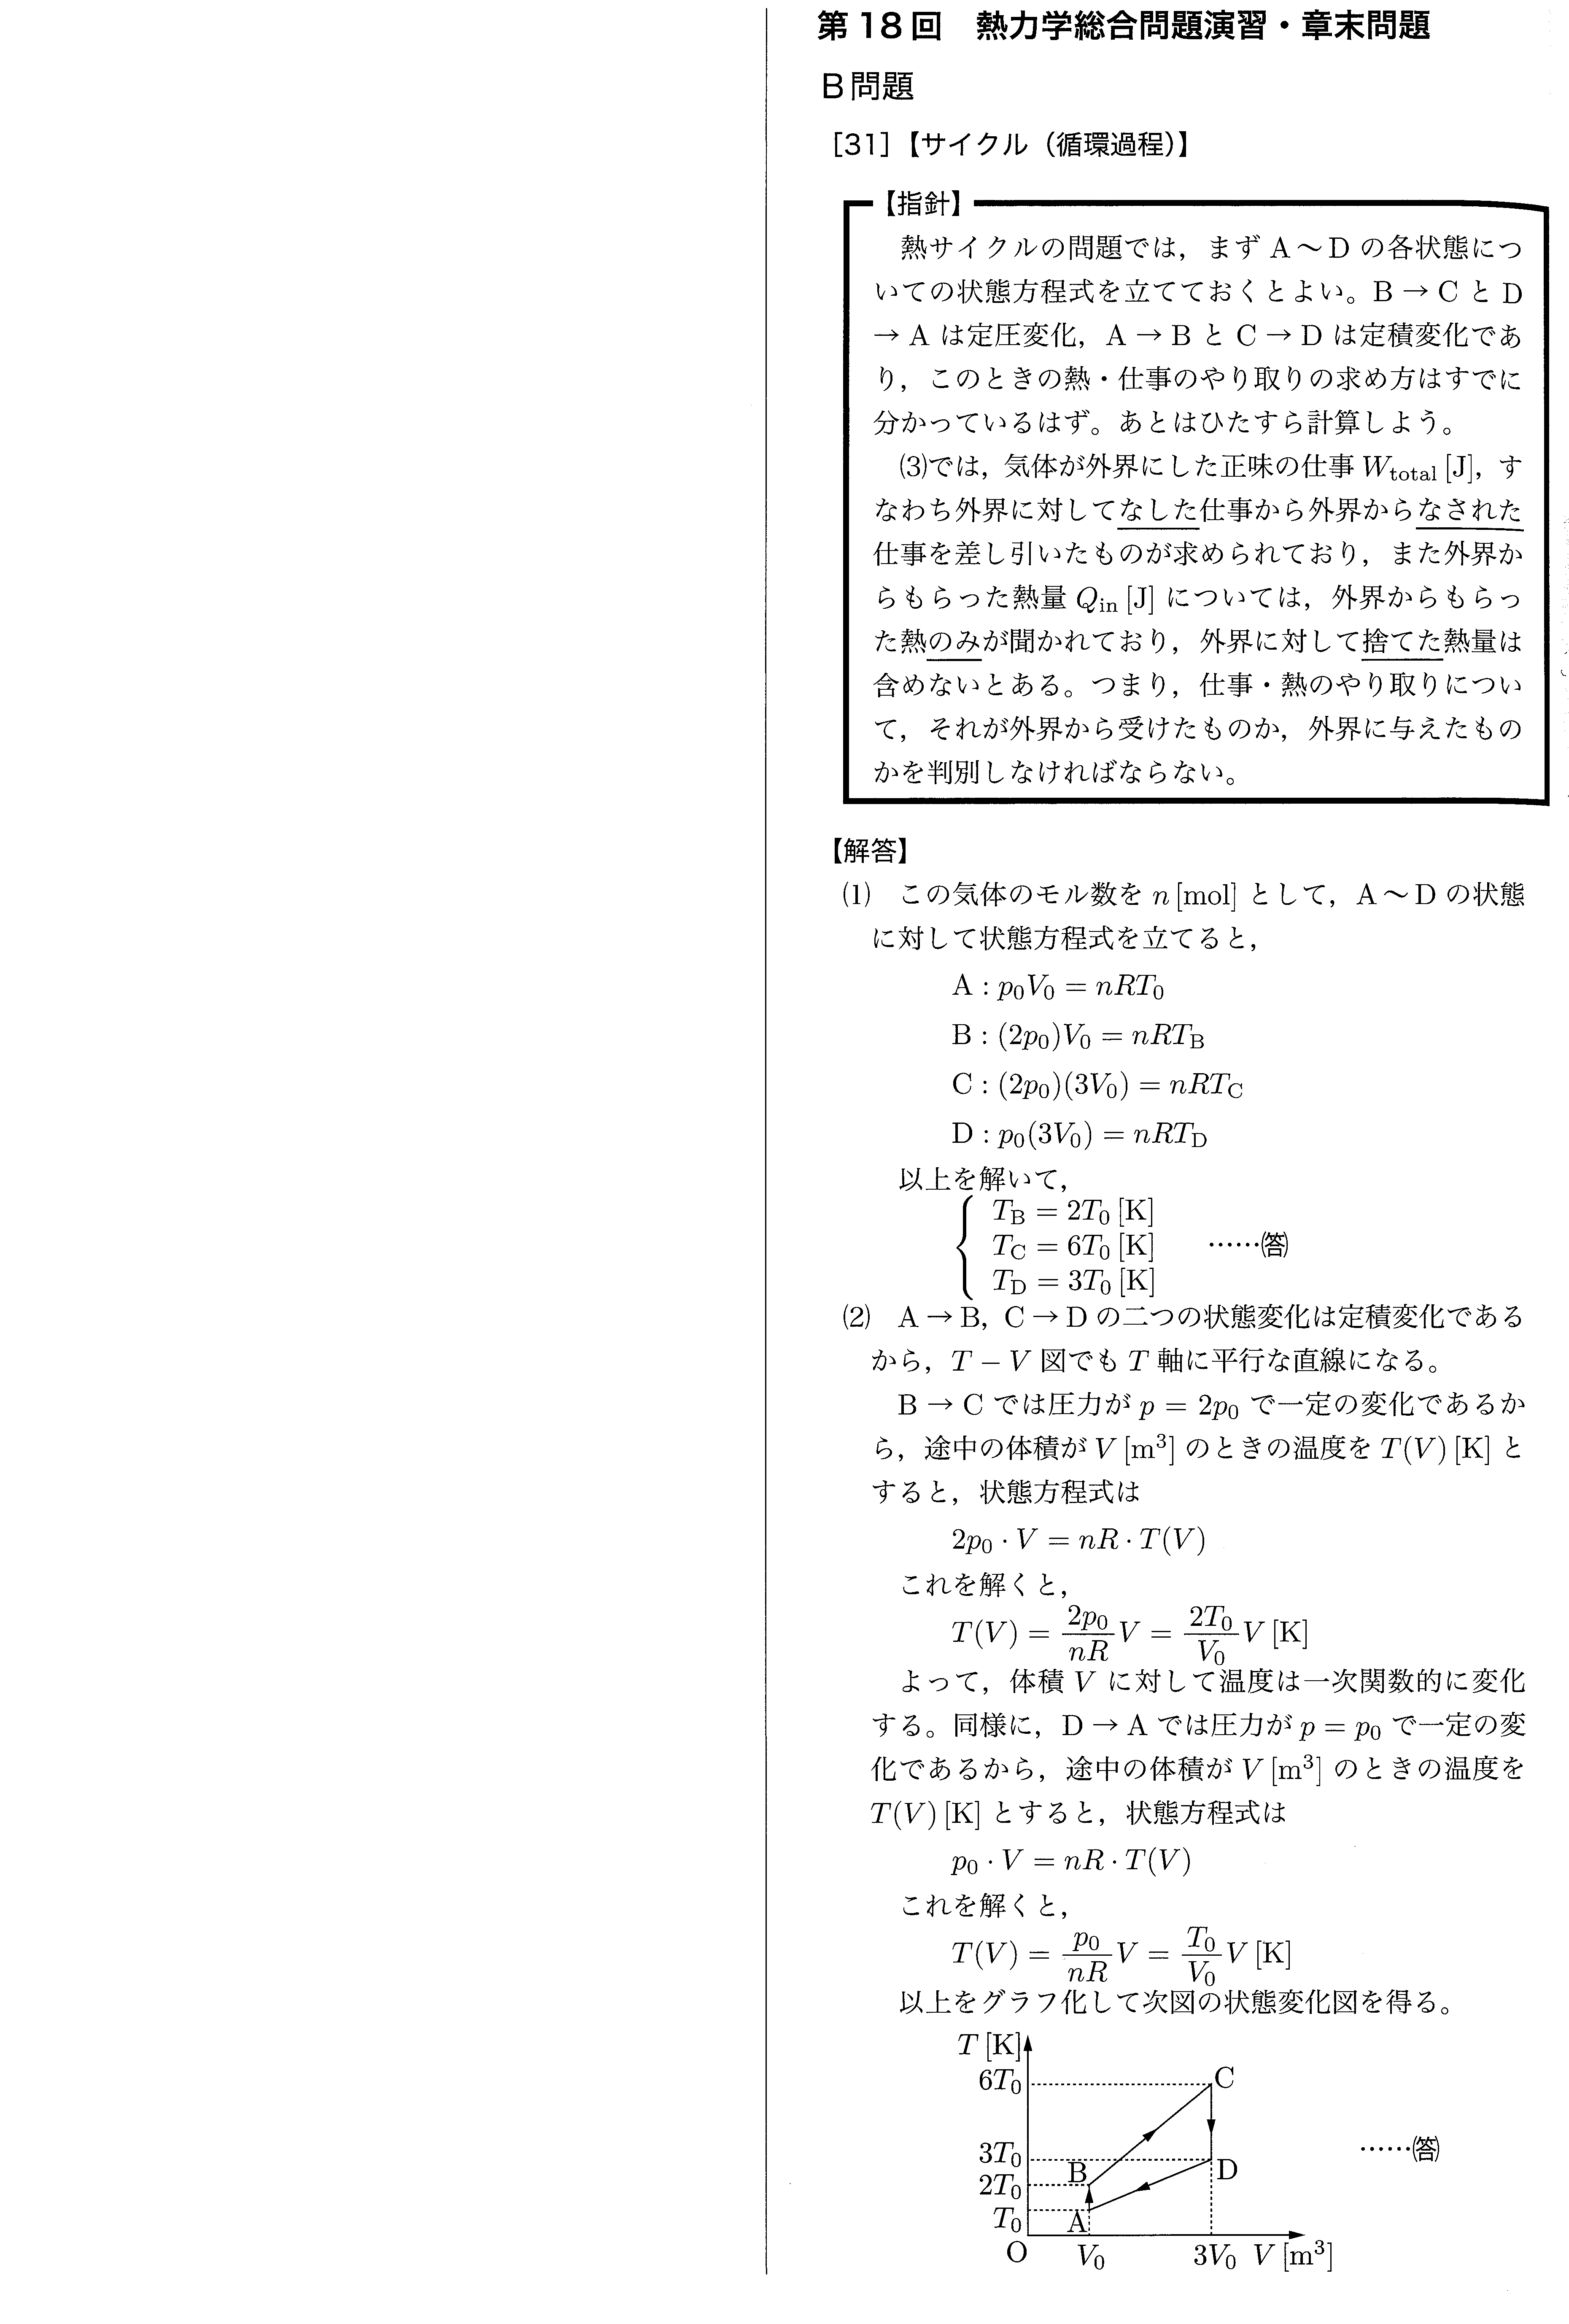
\includegraphics[width=170mm]{prob_p136_2.png}
\end{center}
\end{figure}

\newpage

\begin{figure}[h]
\begin{center}
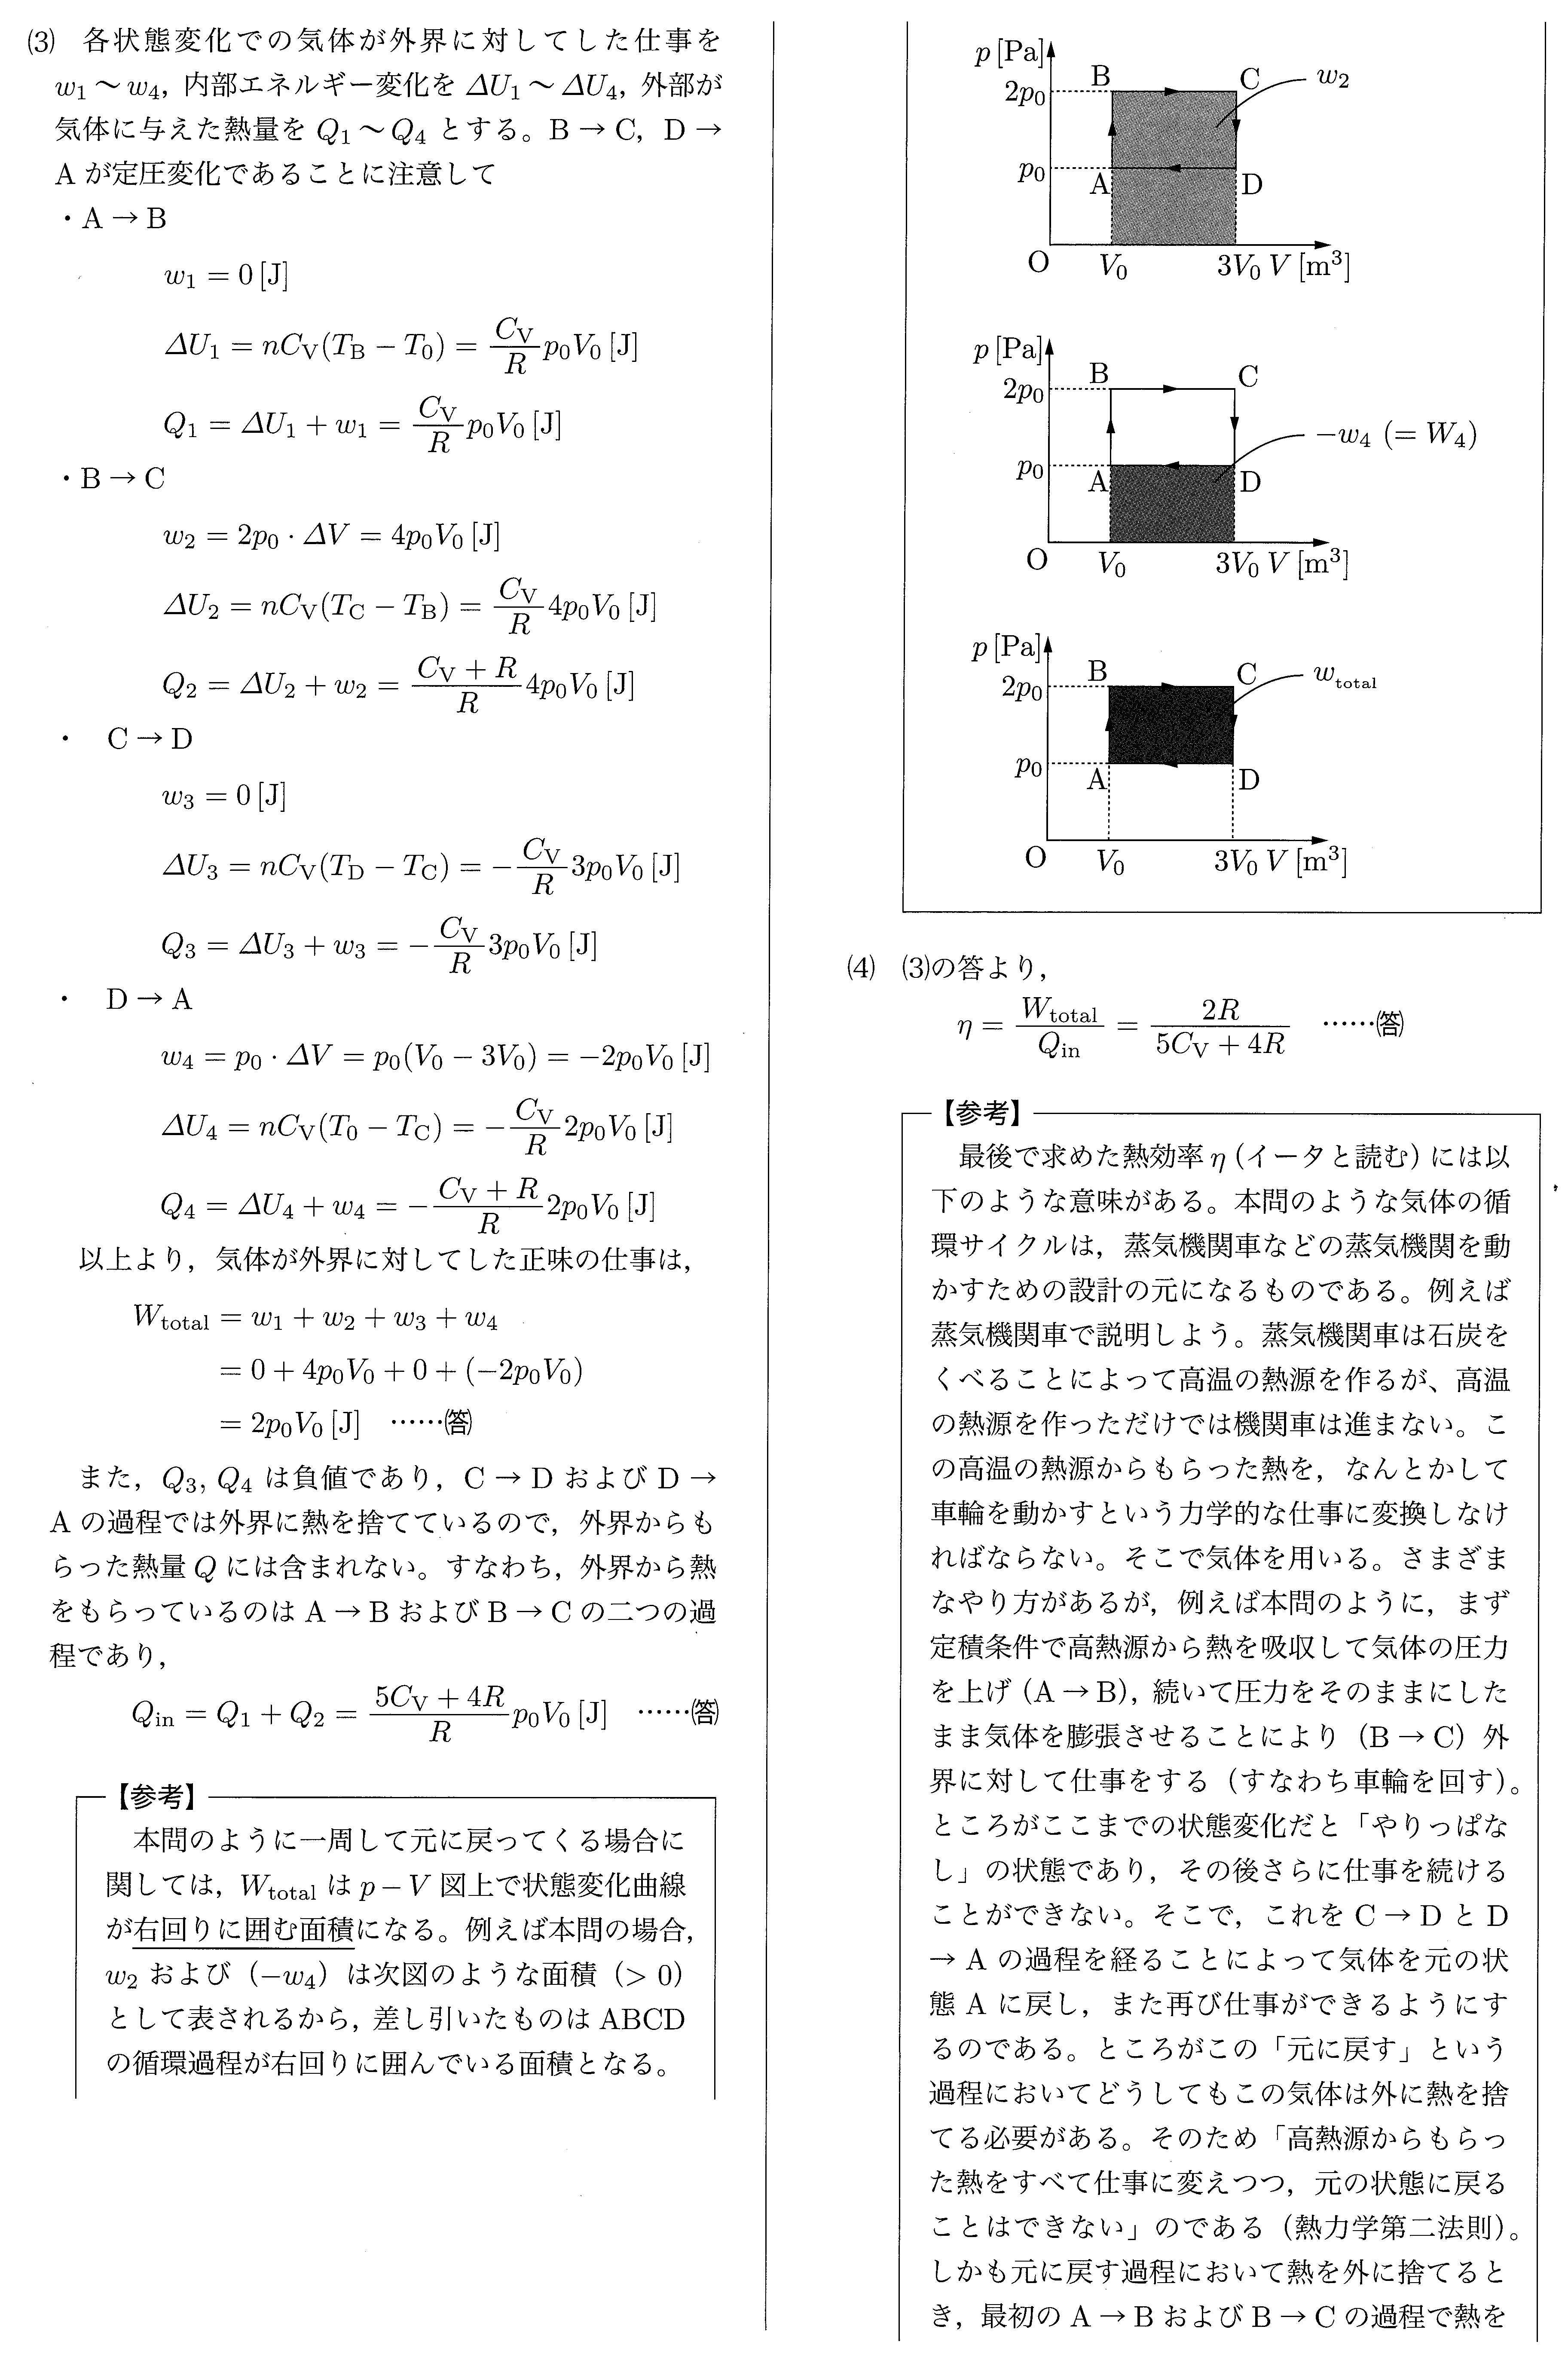
\includegraphics[width=170mm]{prob_p137.png}
\end{center}
\end{figure}


\newpage

\begin{figure}[h]
\begin{center}
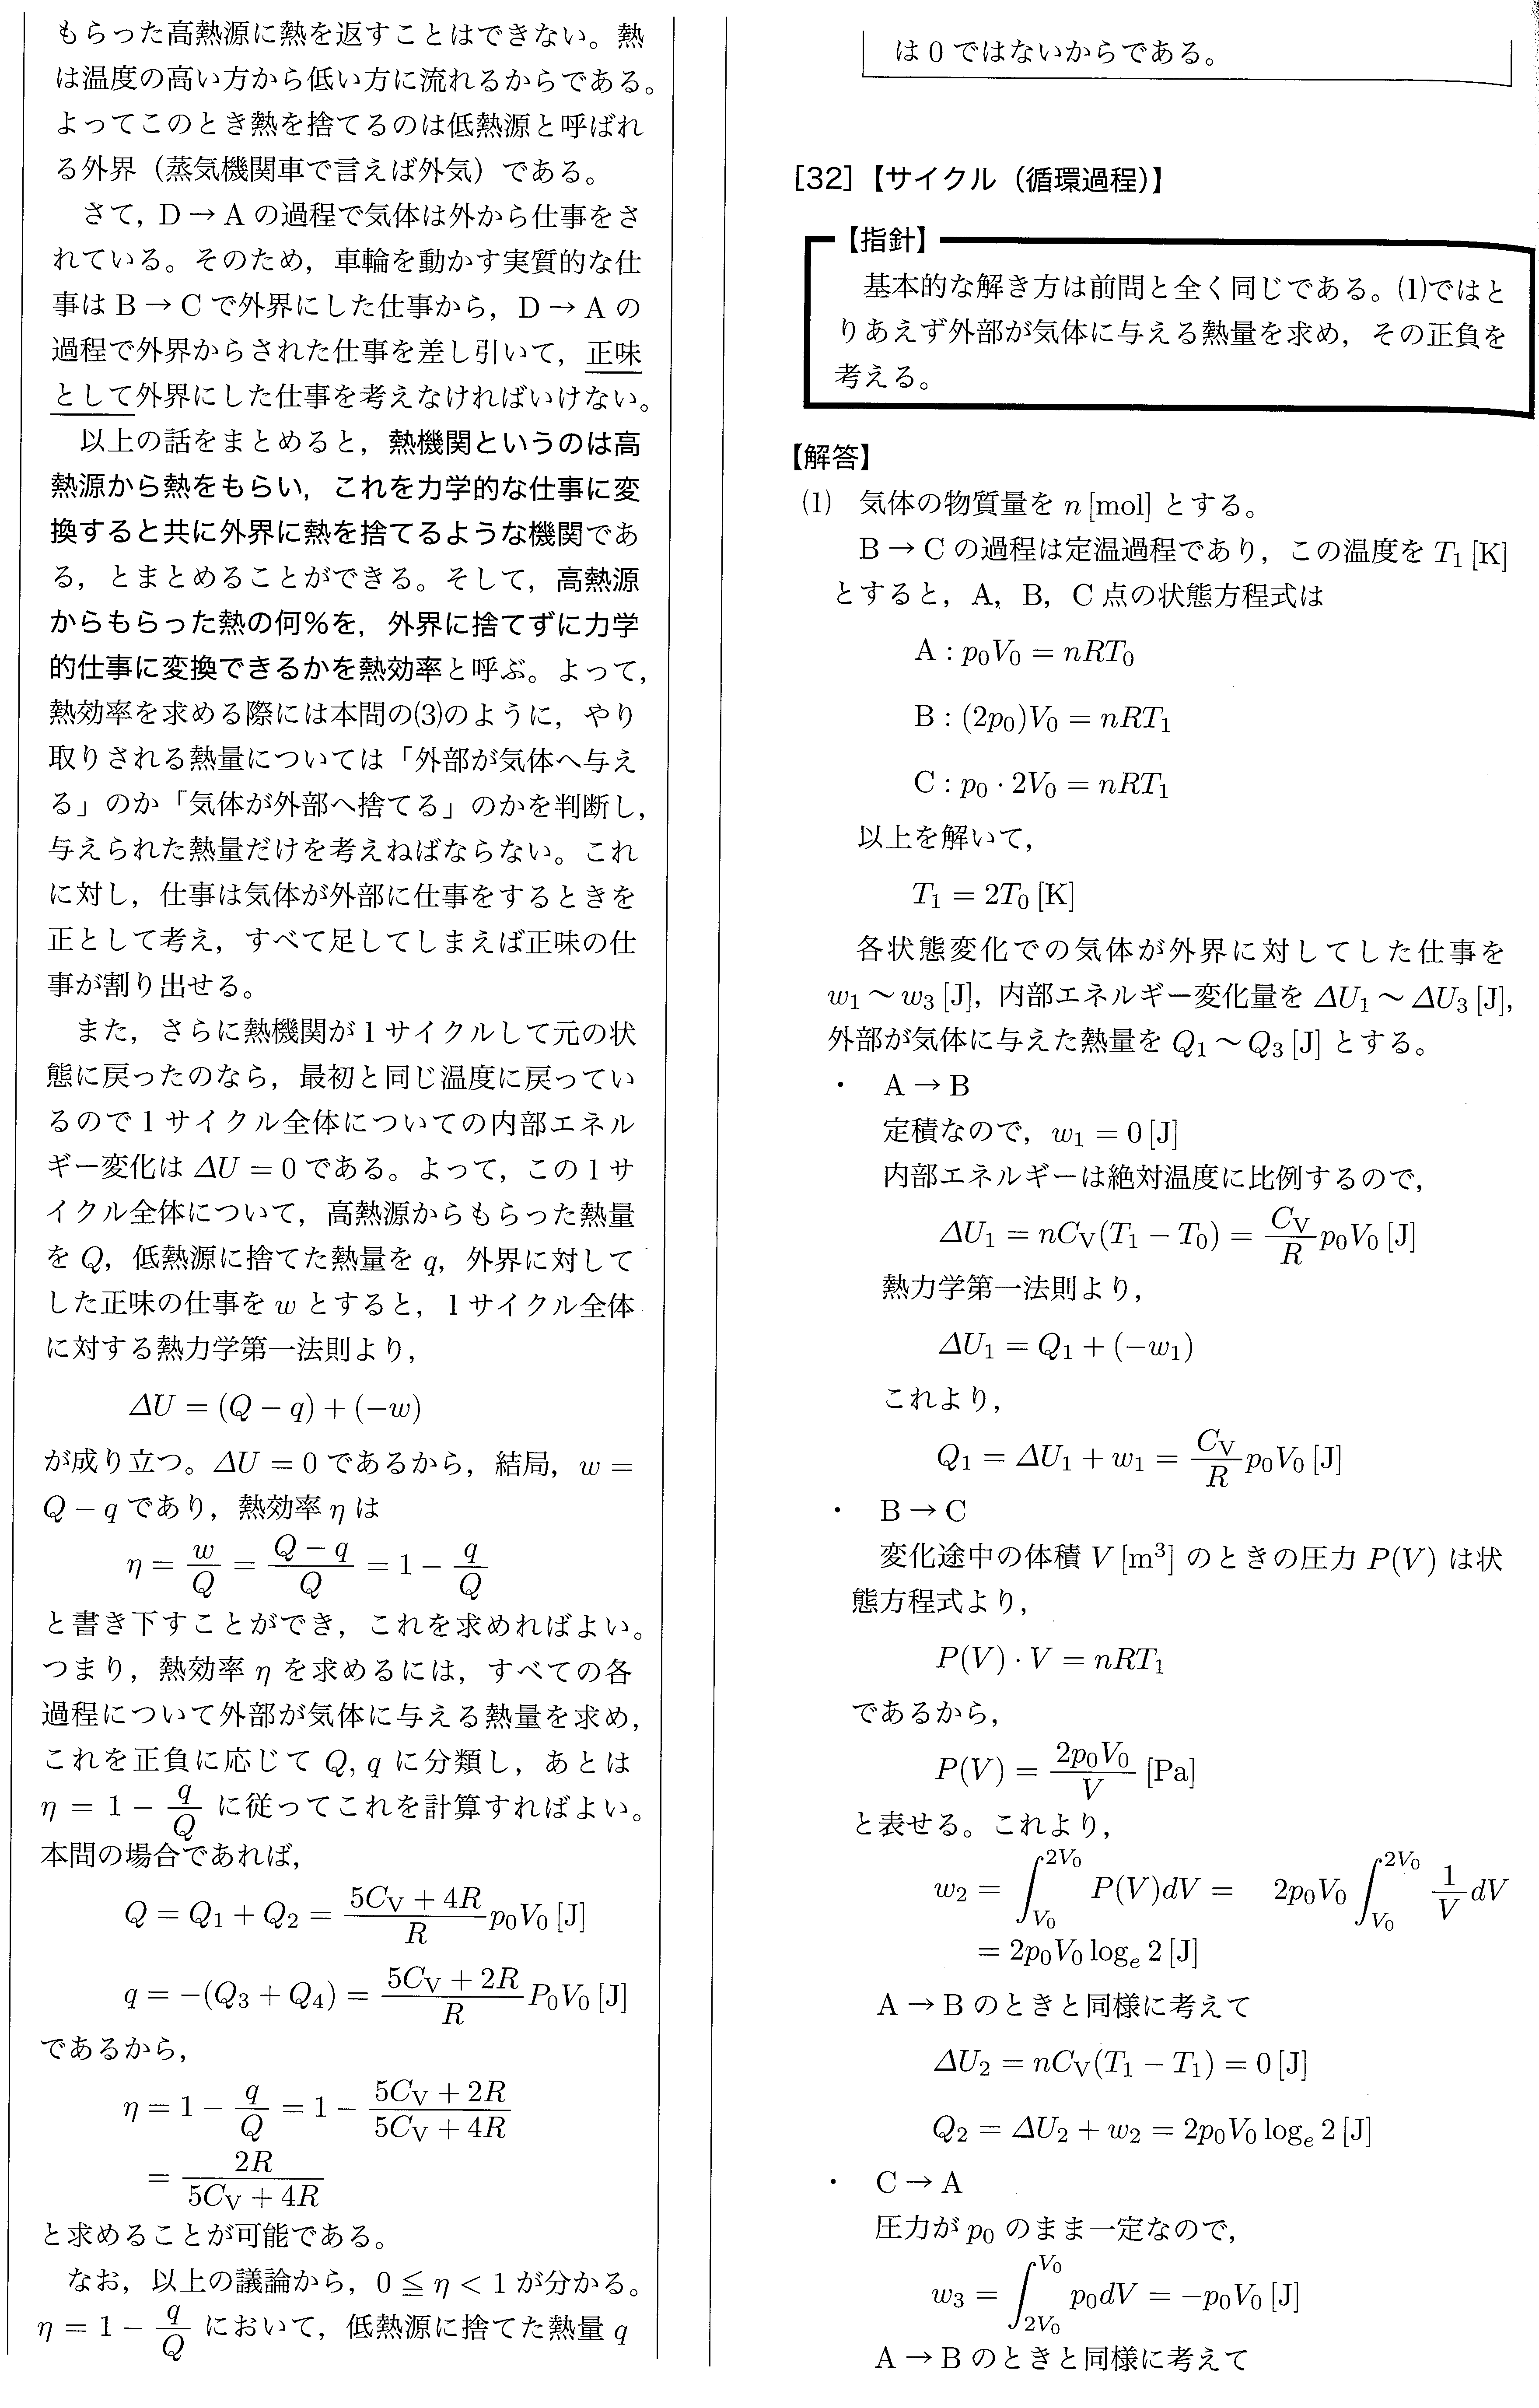
\includegraphics[width=170mm]{prob_p138.png}
\end{center}
\end{figure}

\newpage

\begin{figure}[h]
\begin{center}
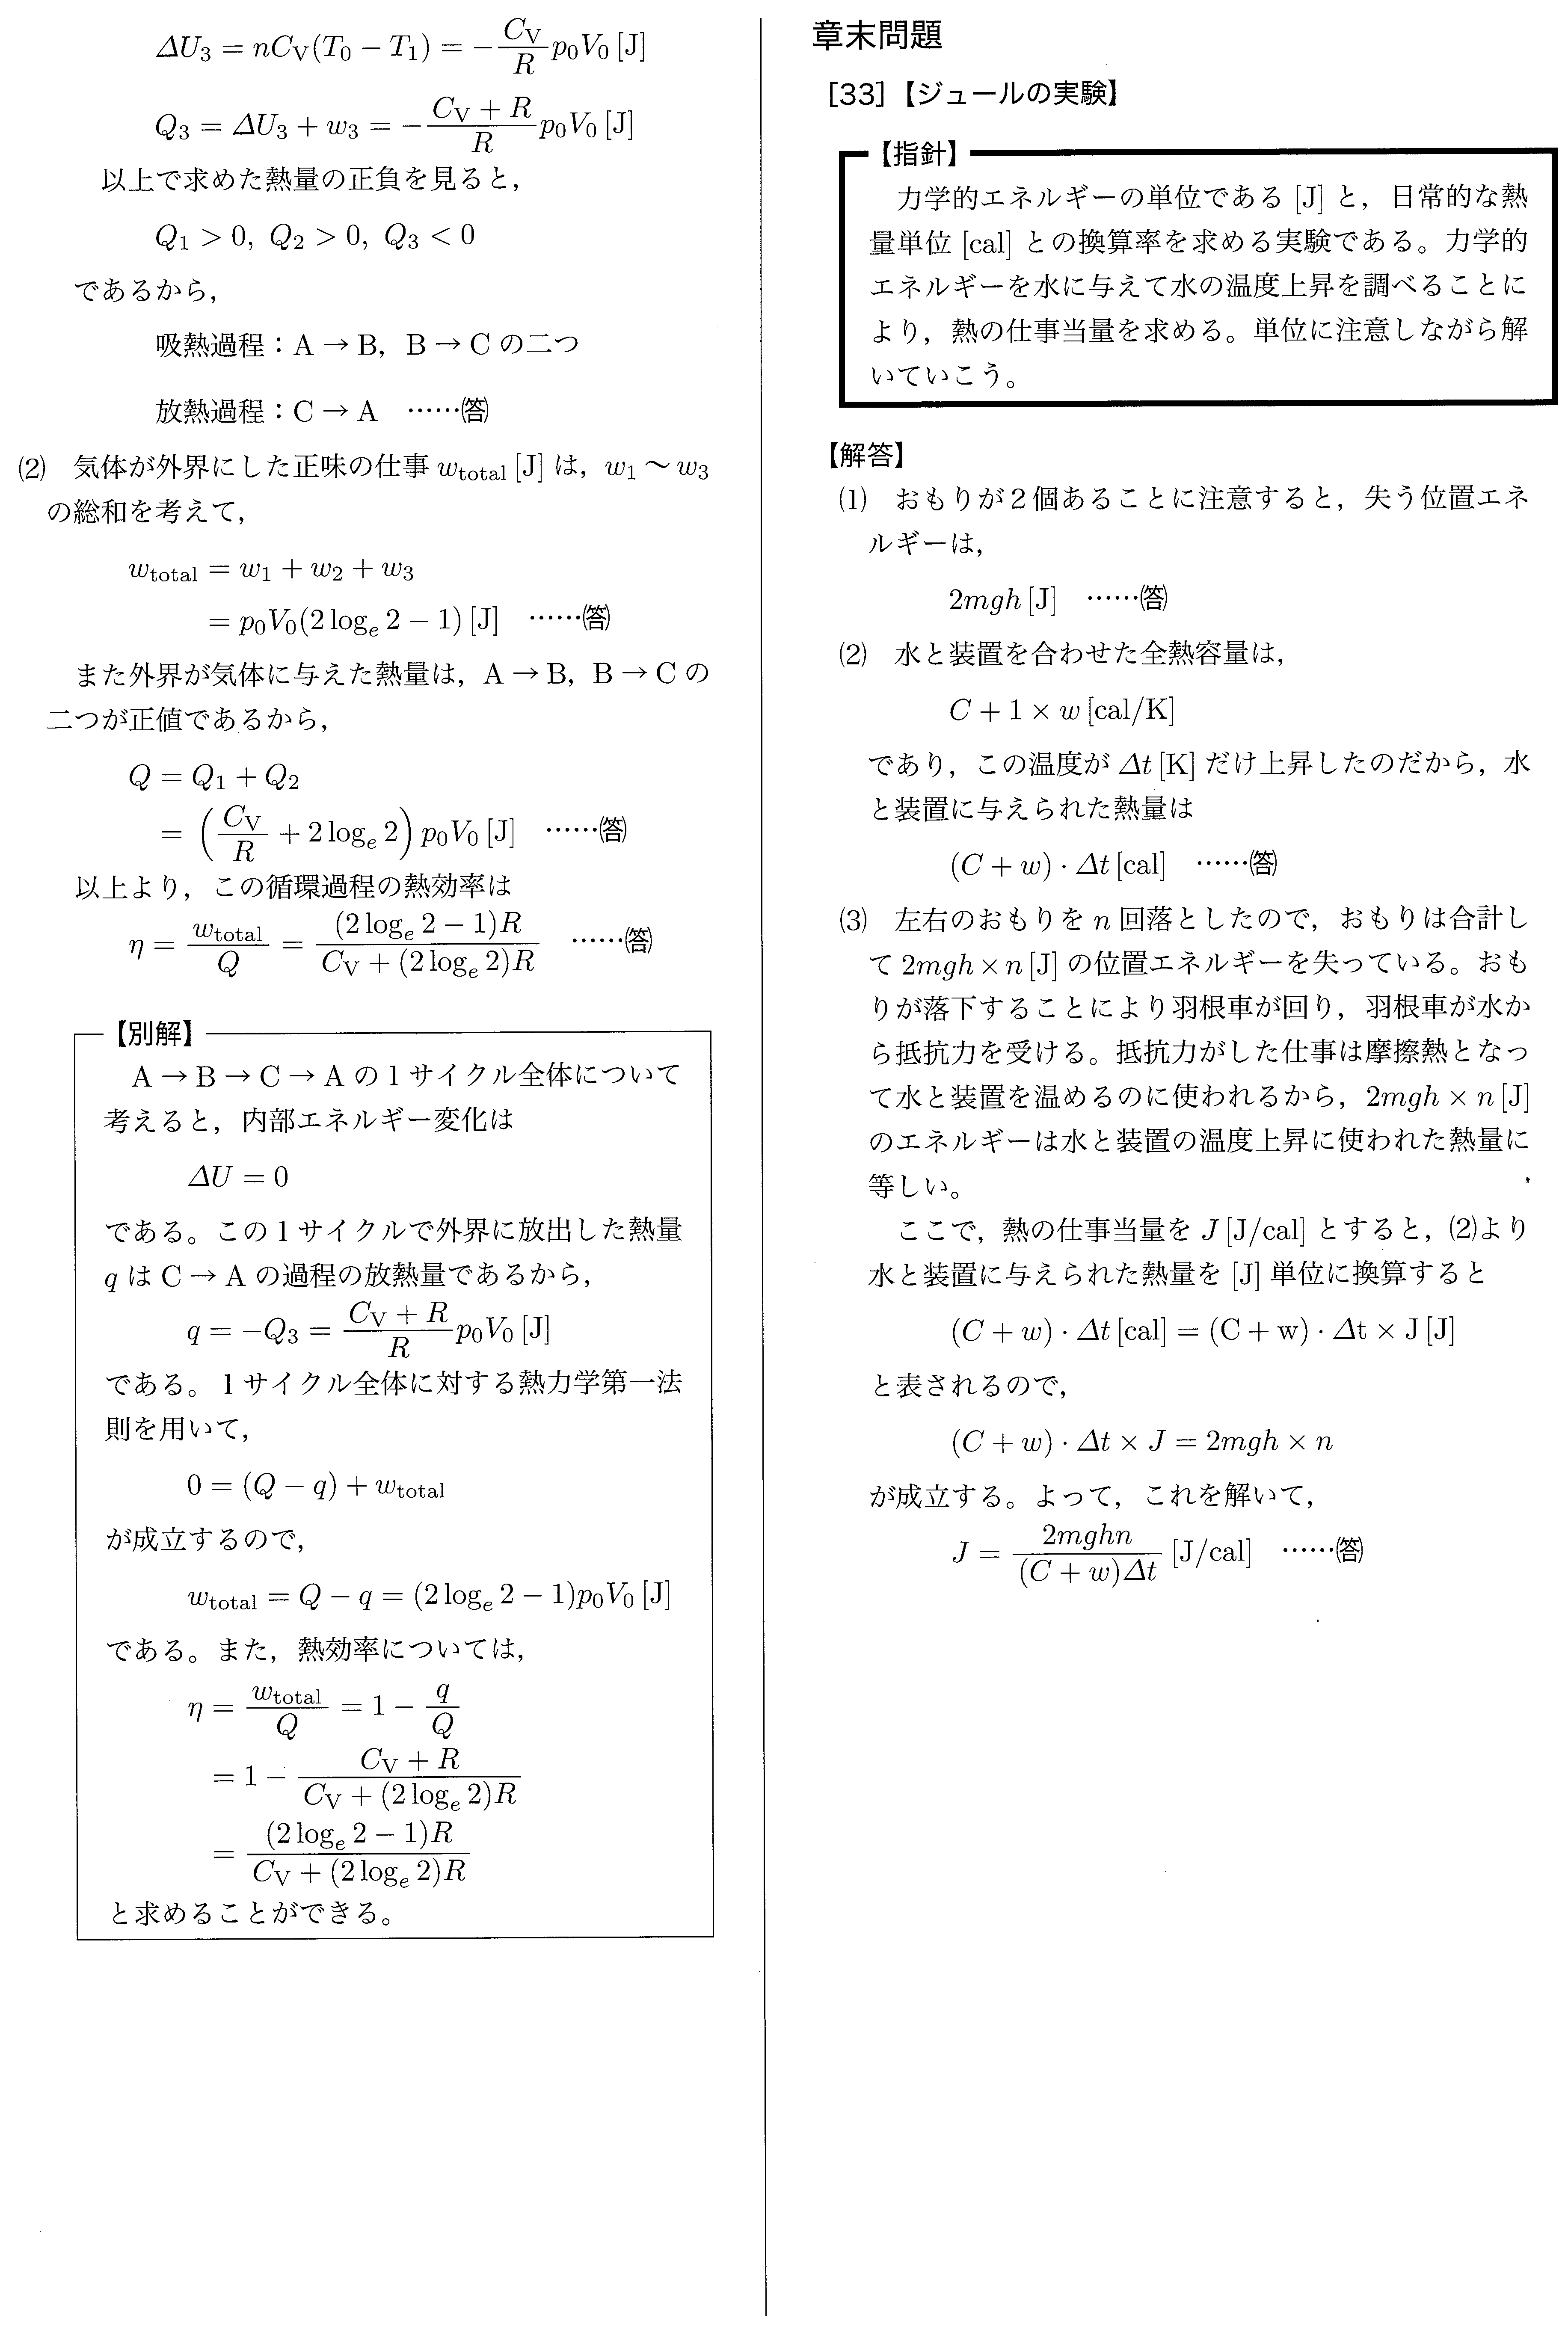
\includegraphics[width=170mm]{prob_p139.png}
\end{center}
\end{figure}

\newpage

\begin{figure}[h]
\begin{center}
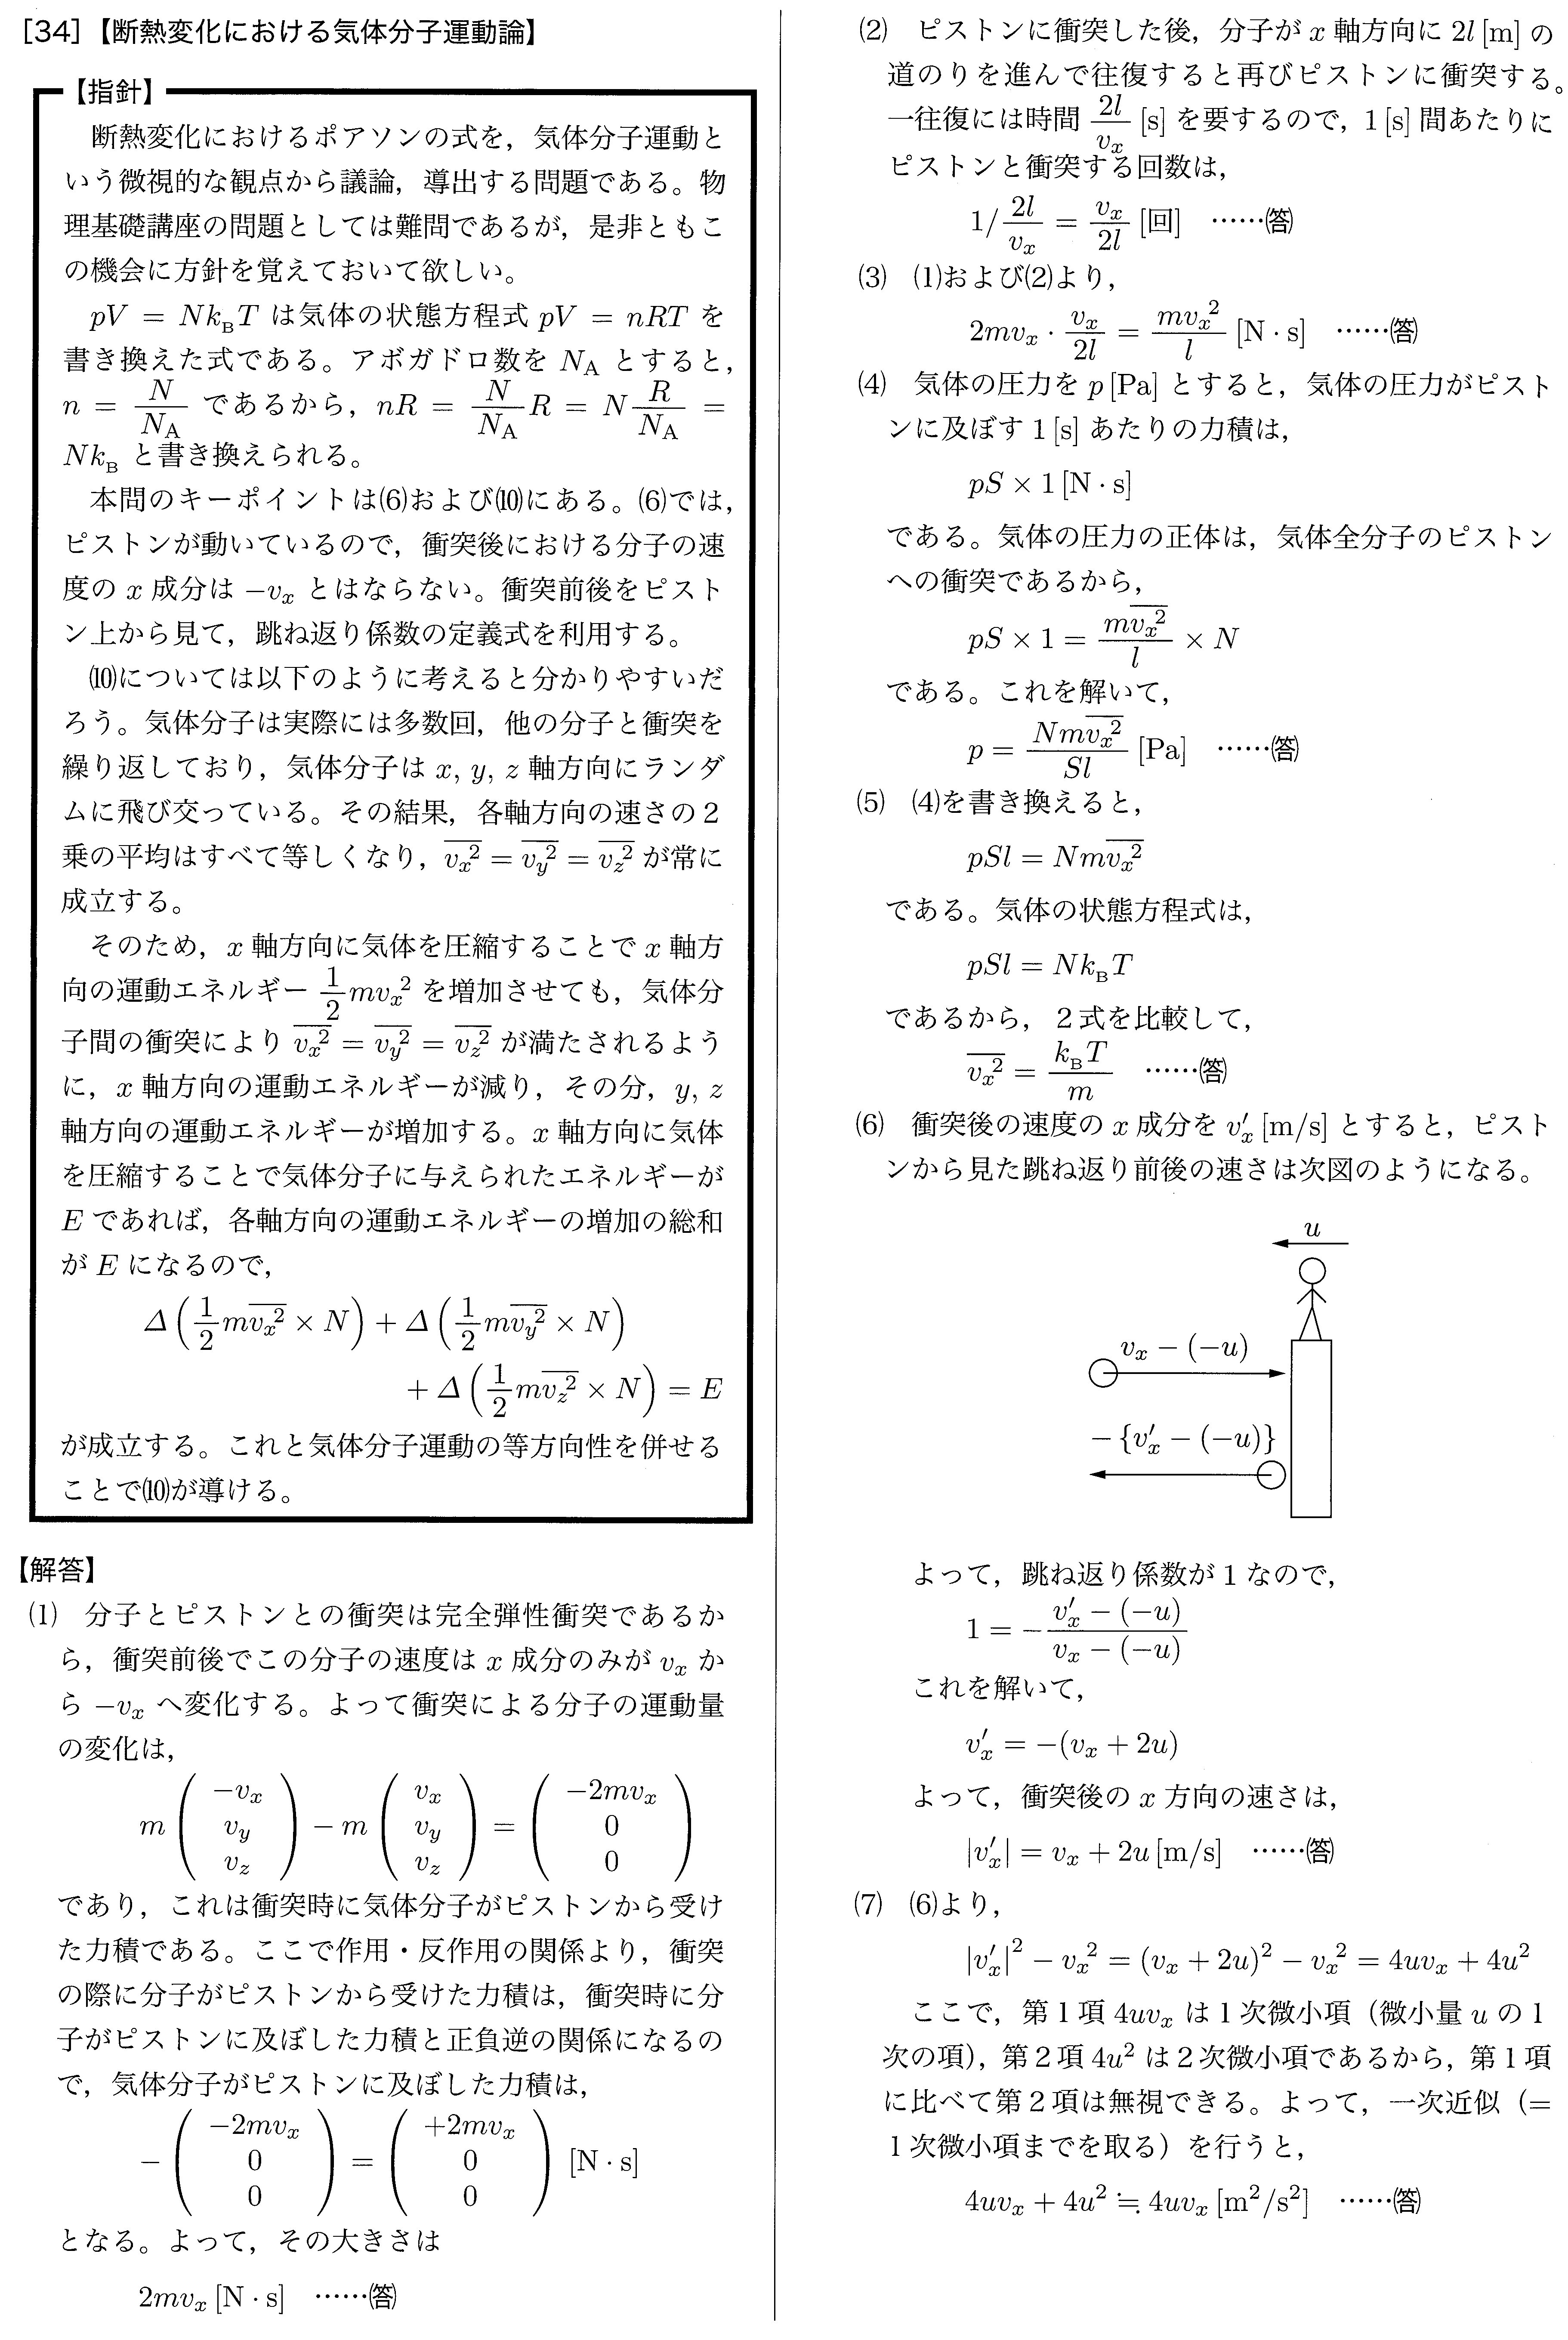
\includegraphics[width=170mm]{prob_p140.png}
\end{center}
\end{figure}

\newpage

\begin{figure}[h]
\begin{center}
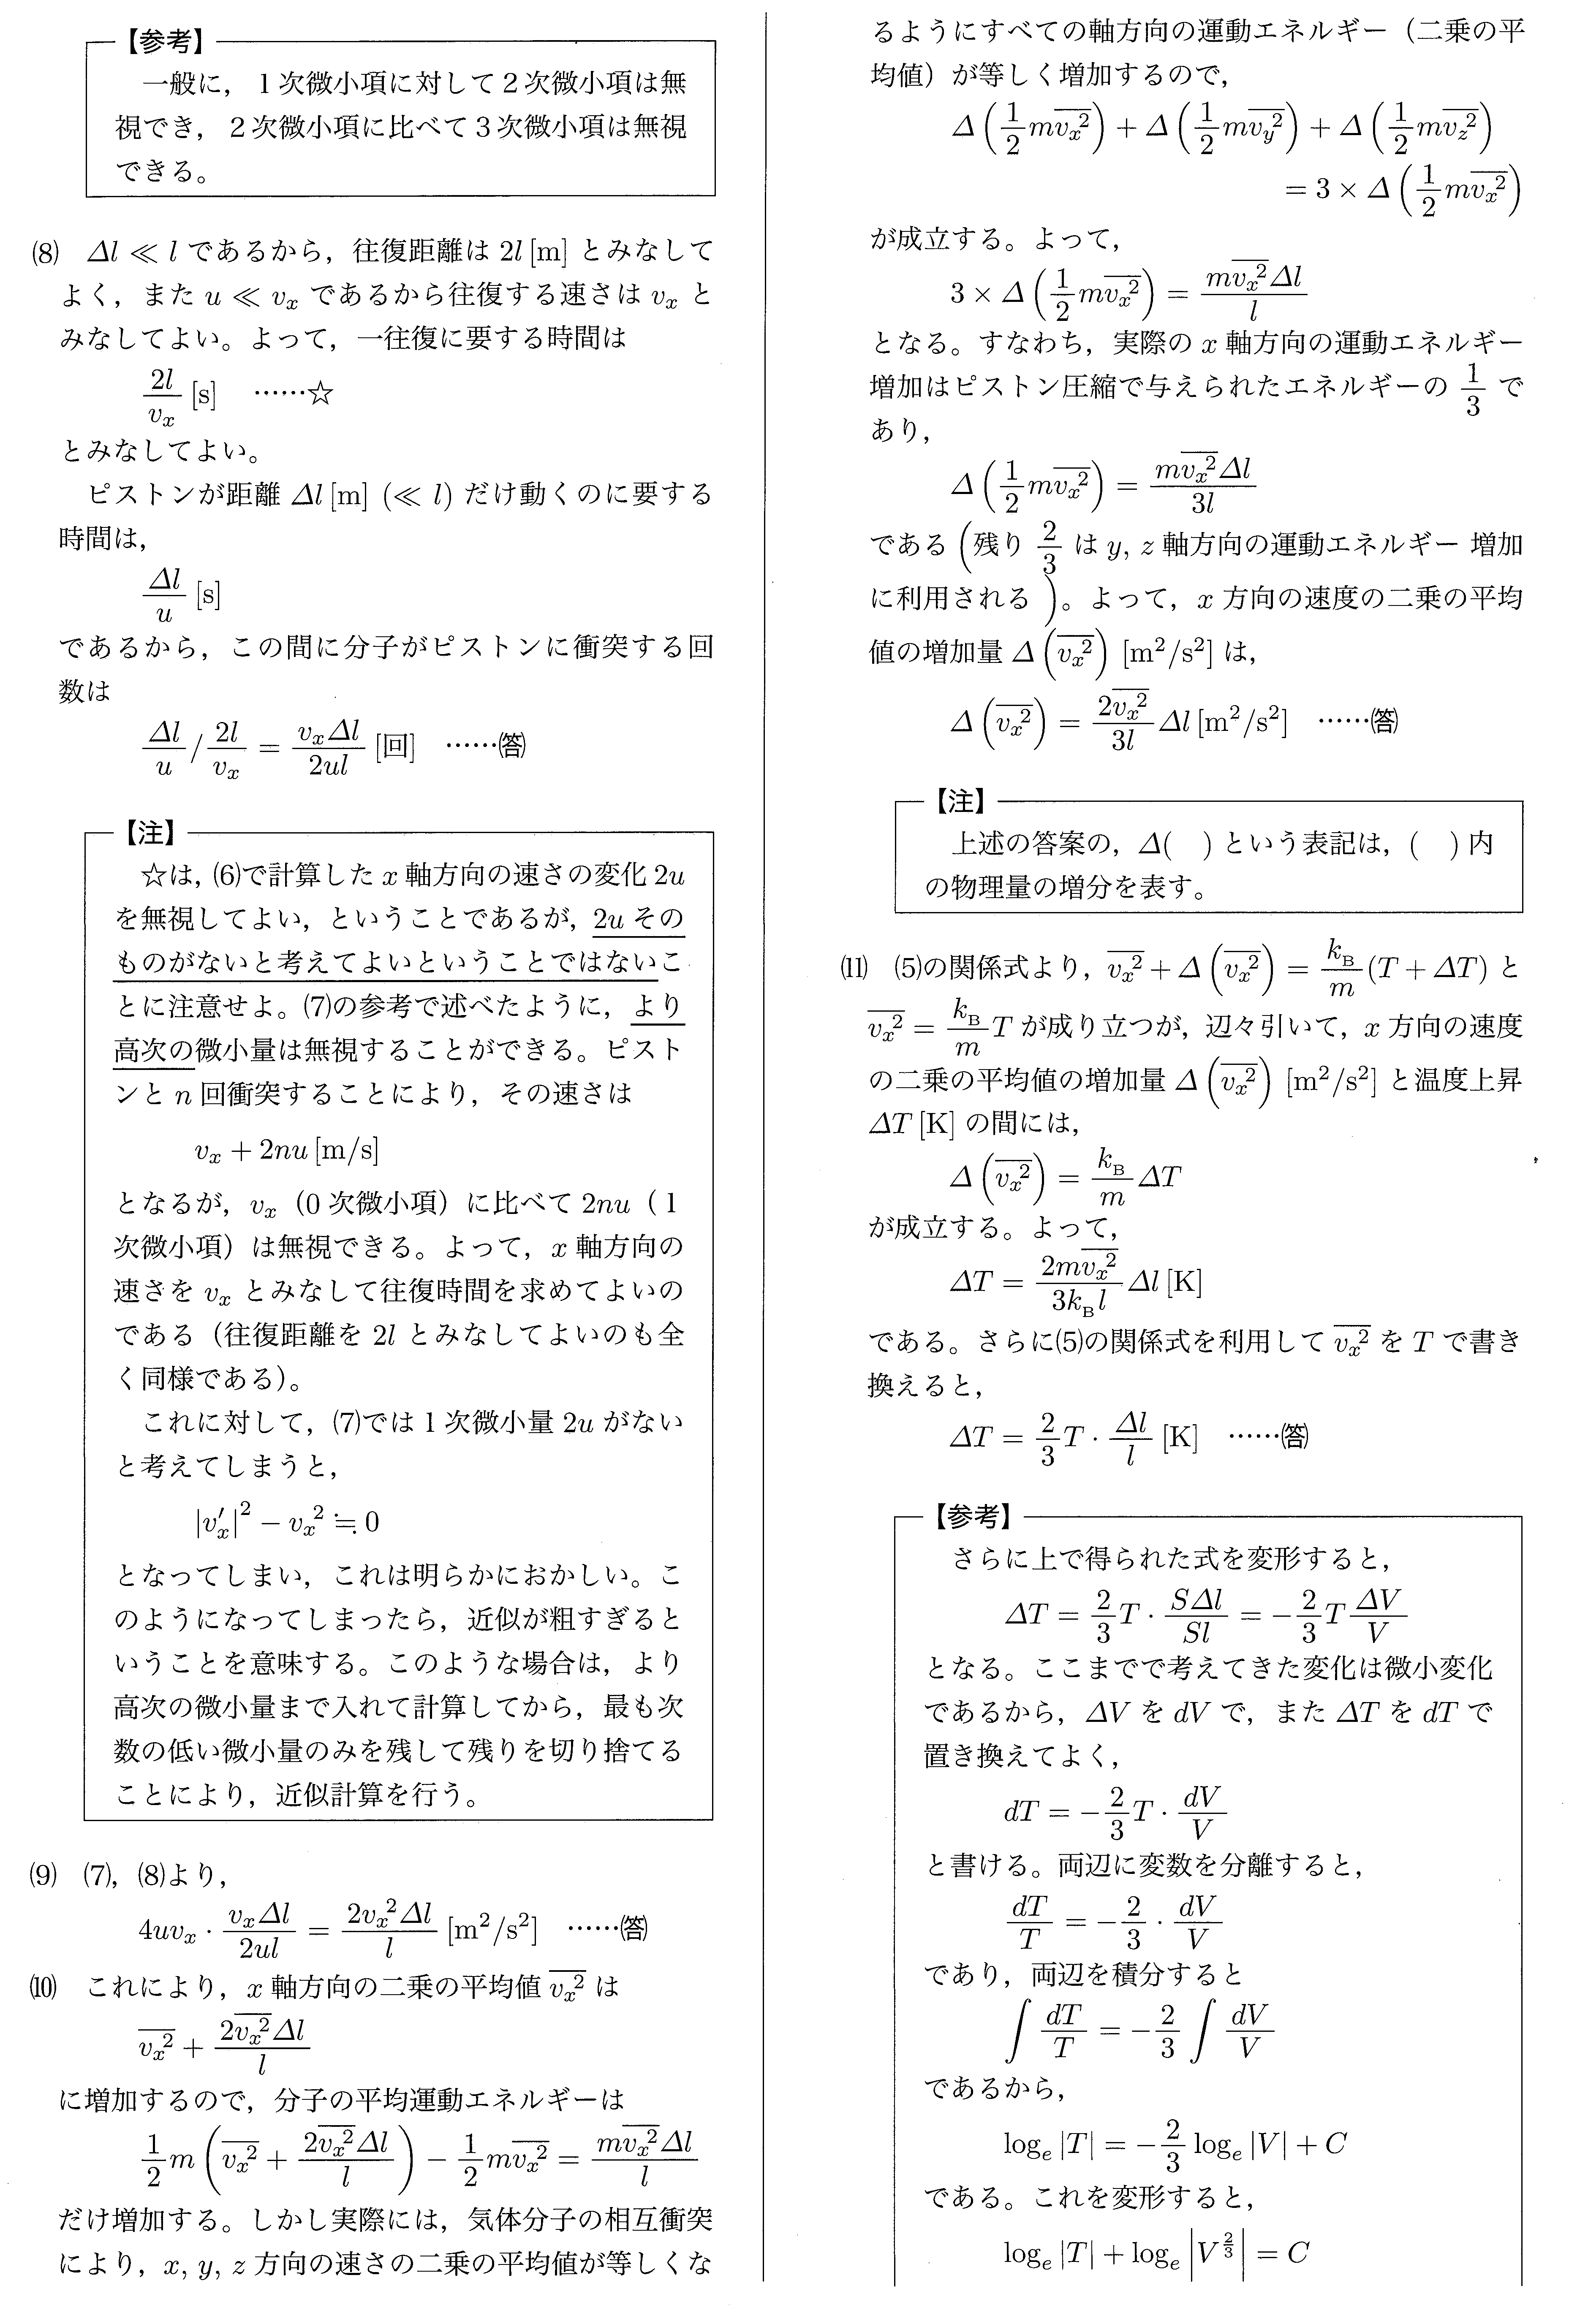
\includegraphics[width=170mm]{prob_p141.png}
\end{center}
\end{figure}

\newpage

\begin{figure}[h]
\begin{center}
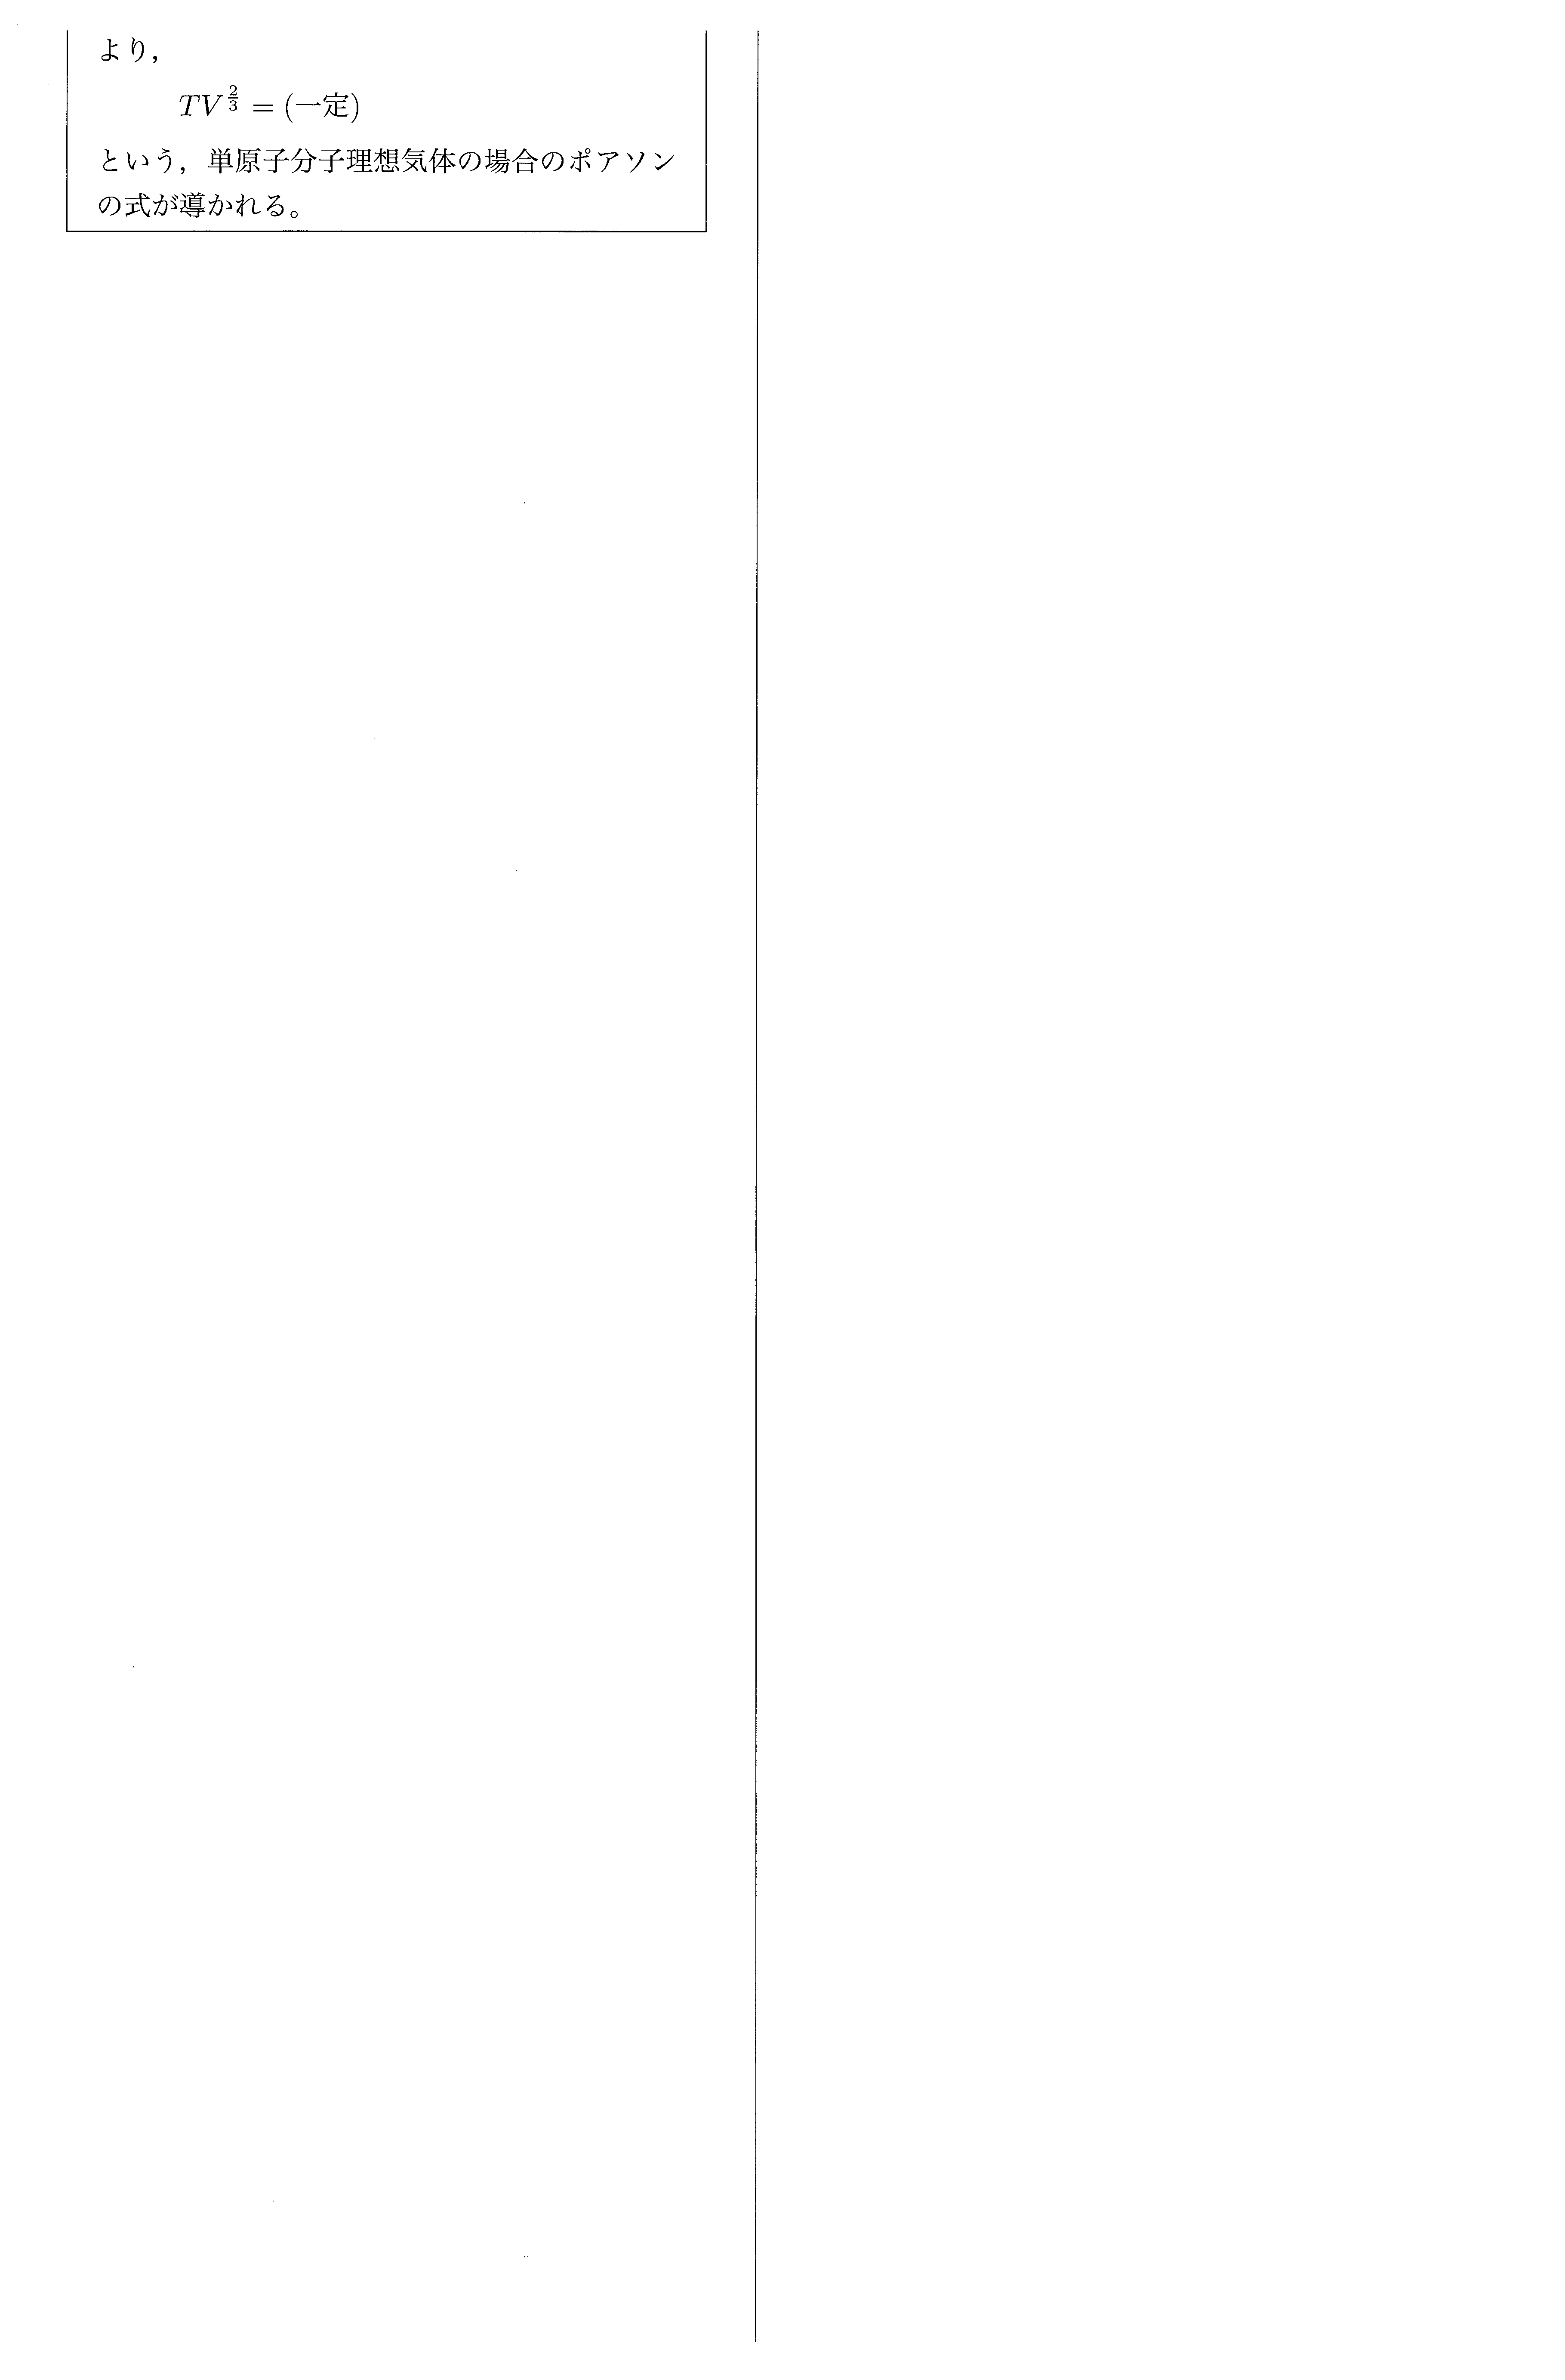
\includegraphics[width=170mm]{prob_p142_1.png}
\end{center}
\end{figure}

\begin{center}
{\Huge \bf 第3章　波動}
\end{center}

\section{正弦波の表式}

\subsection{波長・周期・振動数・波の速さ}
\begin{wrapfigure}[6]{r}[5mm]{80mm}
  \centering
  \vspace{-5mm}
  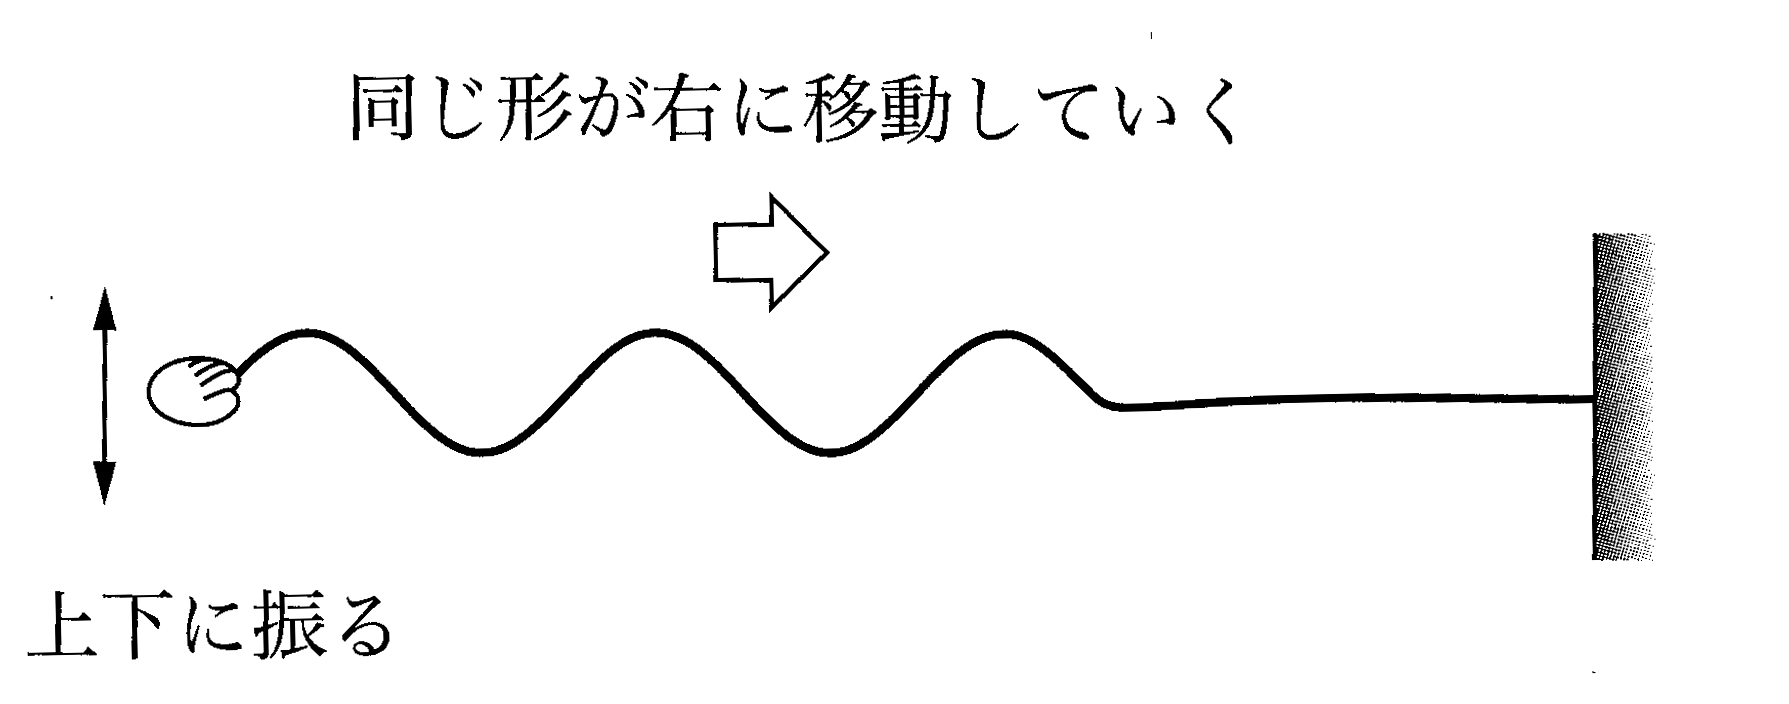
\includegraphics[keepaspectratio,width=80mm]
  {text_p85_fig1.png}
\end{wrapfigure}
壁に糸の一端をくくりつけ，もう一端を手で持ち，壁から離れて上下に振ると，右図のように糸の各部分が上下に振動し，振動の様子が右側に伝播していく．
このように何かしらの物理量が空間的に伝播していく現象を{\bf 波動}，または単に{\bf 波}と呼び，波を伝える物質を{\bf 媒質}と呼ぶ．
媒質はその場で振動し，振動の方向が波の伝播方向と垂直な波を{\bf 横波}と呼び，伝播方向と平行な波を{\bf 縦波}と呼ぶ．
先ほどの例は糸が媒質となっている横波である．
まずは横波について考えていこう．

\begin{wrapfigure}[20]{r}[5mm]{90mm}
  \centering
  \vspace{-5mm}
  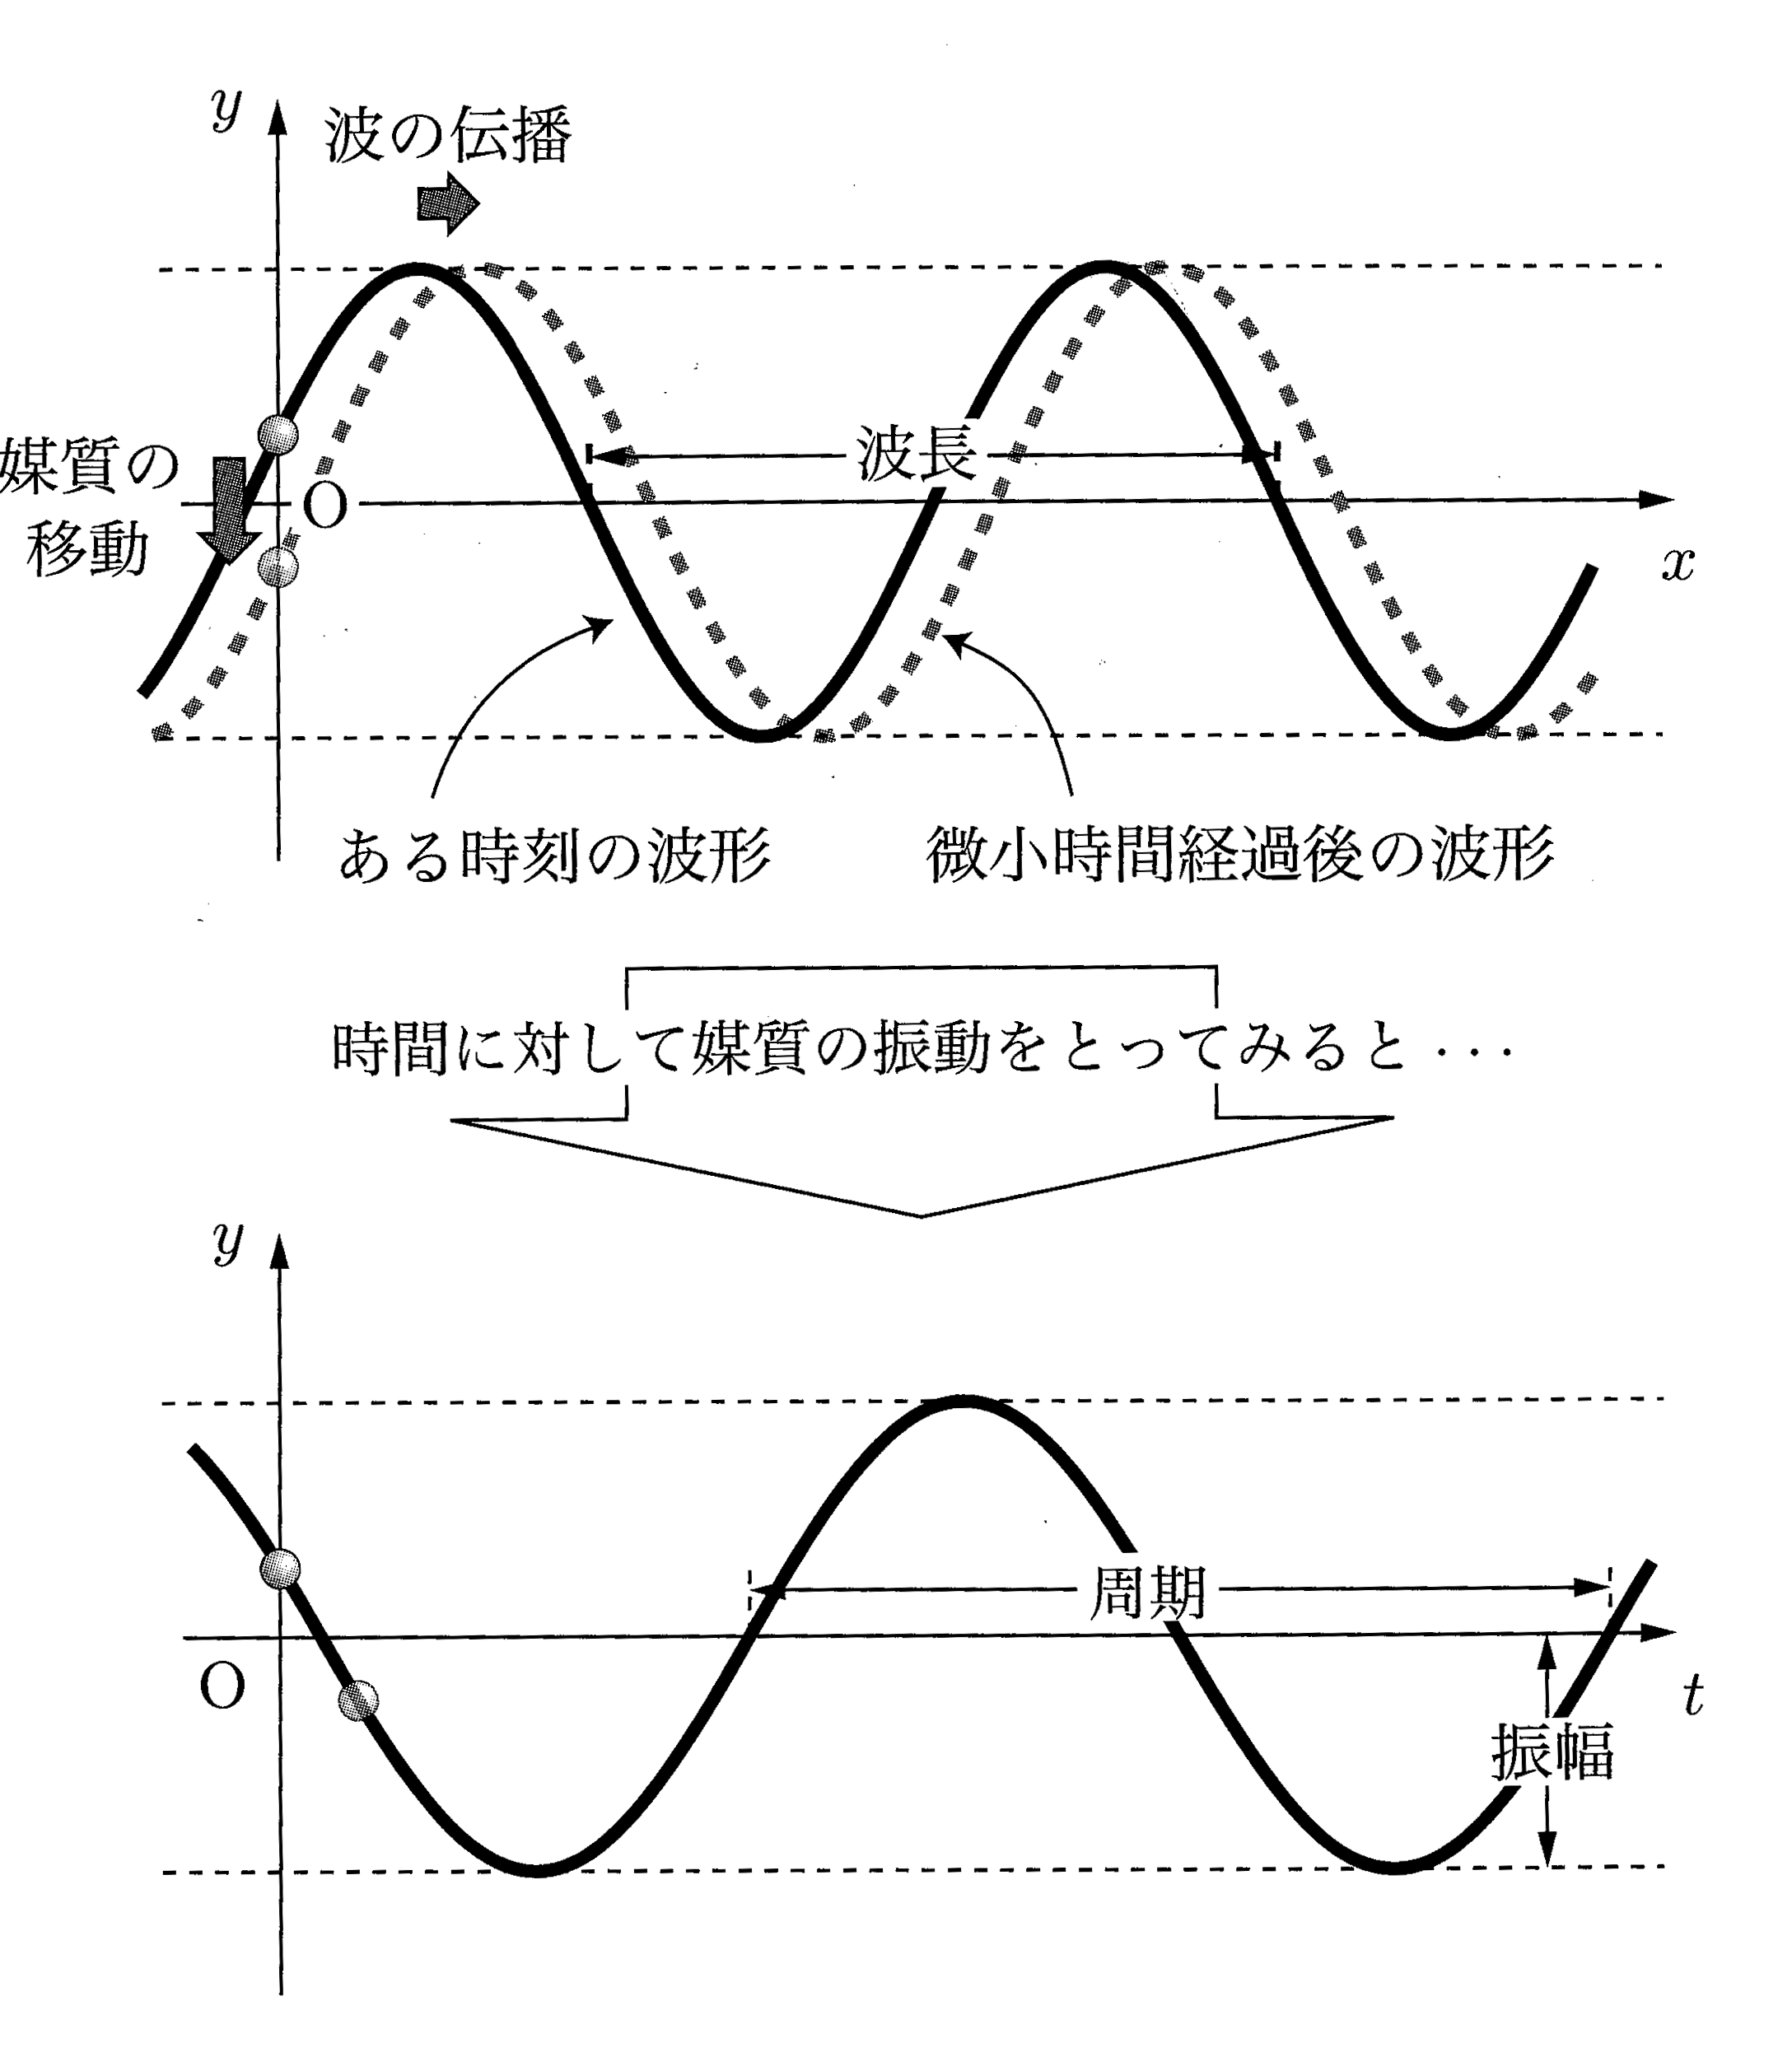
\includegraphics[keepaspectratio,width=90mm]
  {text_p85_fig2.png}
\end{wrapfigure}
伝播していく波の形が三角関数（$\sin$カーブ）である波を{\bf 正弦波}と呼ぶ．
伝播方向を$x$軸と設定し，ある時刻における$x$軸上の各点の変位を$y$[m]で表した$y-x$グラフは右図の実線のように表現できる．
$\sin$カーブ1つ分の長さを{\bf 波長}と呼び，変位の最大の大きさを{\bf 振幅}と呼ぶ．

各媒質は単振動をしていて，この単振動の周期と波の形が元の形に戻るまでの周期は一致する．
各媒質が単位時間あたりに何回振動するかを{\bf 振動数}と呼び，単位は{\bf [/s]=[Hz]（ヘルツ）}で表す．
周期を$T$[s]とすれば，振動数$f$[Hz]と$T$の間には
\[\mbox{\boldmath $f=\dfrac{1}{T}$}\]
が成立する．
また，波長を$\lambda$[m]とすれば，振動1回あたり$\lambda$[m]だけ波形が移動するので，波の伝播速度$v$[m/s]は
\[\mbox{\boldmath $v=f\lambda $}\]
となる．これを波の基本式という．

\begin{matome}{正弦波}
 \hspace{3mm} 正弦波：各質点が単振動をしており，$\sin$カーブの波形が伝わっていく波動\\
\hspace{3mm} 媒質：波動を伝える物質．その点で上下振動しているのみで，波形のみがずれていく．\\
\hspace{3mm} 波長：ある瞬間に波の形を見た際に，同一変異が現れる距離\\
\hspace{3mm} 周期：ある媒質の上下振動に着目したときに媒質が同じ状態に戻るまでの時間，もしくは波形が一波長分ずれるのに要する時間\\
\hspace{4mm} 波の伝播速度\hspace{5mm}$v=f\lambda$\hspace{2mm}[m/s] \hspace{10mm} 波の振動数\hspace{5mm} $f=\dfrac{1}{T}$\hspace{2mm}[Hz]
 \end{matome}



\subsection{$y-x$グラフによる正弦波の一般式の導出}
ある波動の変位を式で表す場合には，どの場所の，いつの時刻の変位かの指定が必要であるから，波の変位$y$[m]は{\bf 位置} \mbox{\boldmath $x$}{\bf [m]と時刻}\mbox{\boldmath $t$} {\bf [s]の2変数関数}\mbox{\boldmath $y(x,t)$} {\bf[m]}となる．
そのため，この正弦波の方程式を直接立てることは非常に難しい．

そこで，正弦波の表式$y(x,t)$を得るには，まず片方の変数を固定したとき（通常は0とした場合）の表式を作り，その後，もう片方の変数を動かして，任意の$x,t$に対する変位を決定する．

どちらの変数を固定するかで2通りあるが，ここではまず，時刻$t$[s]を先に固定した場合を考える．
例えば時刻$t$[s]を$t=0$[s]に固定した場合，$y(x,0)$が表すものは時刻$t=0$[s]における波形である．
よって，与えられた時刻$t=0$[s]における波形グラフを具体的数式で表せば，$y(x,0)$が得られる．

\begin{wrapfigure}[12]{r}[5mm]{100mm}
  \centering
  \vspace{-5mm}
  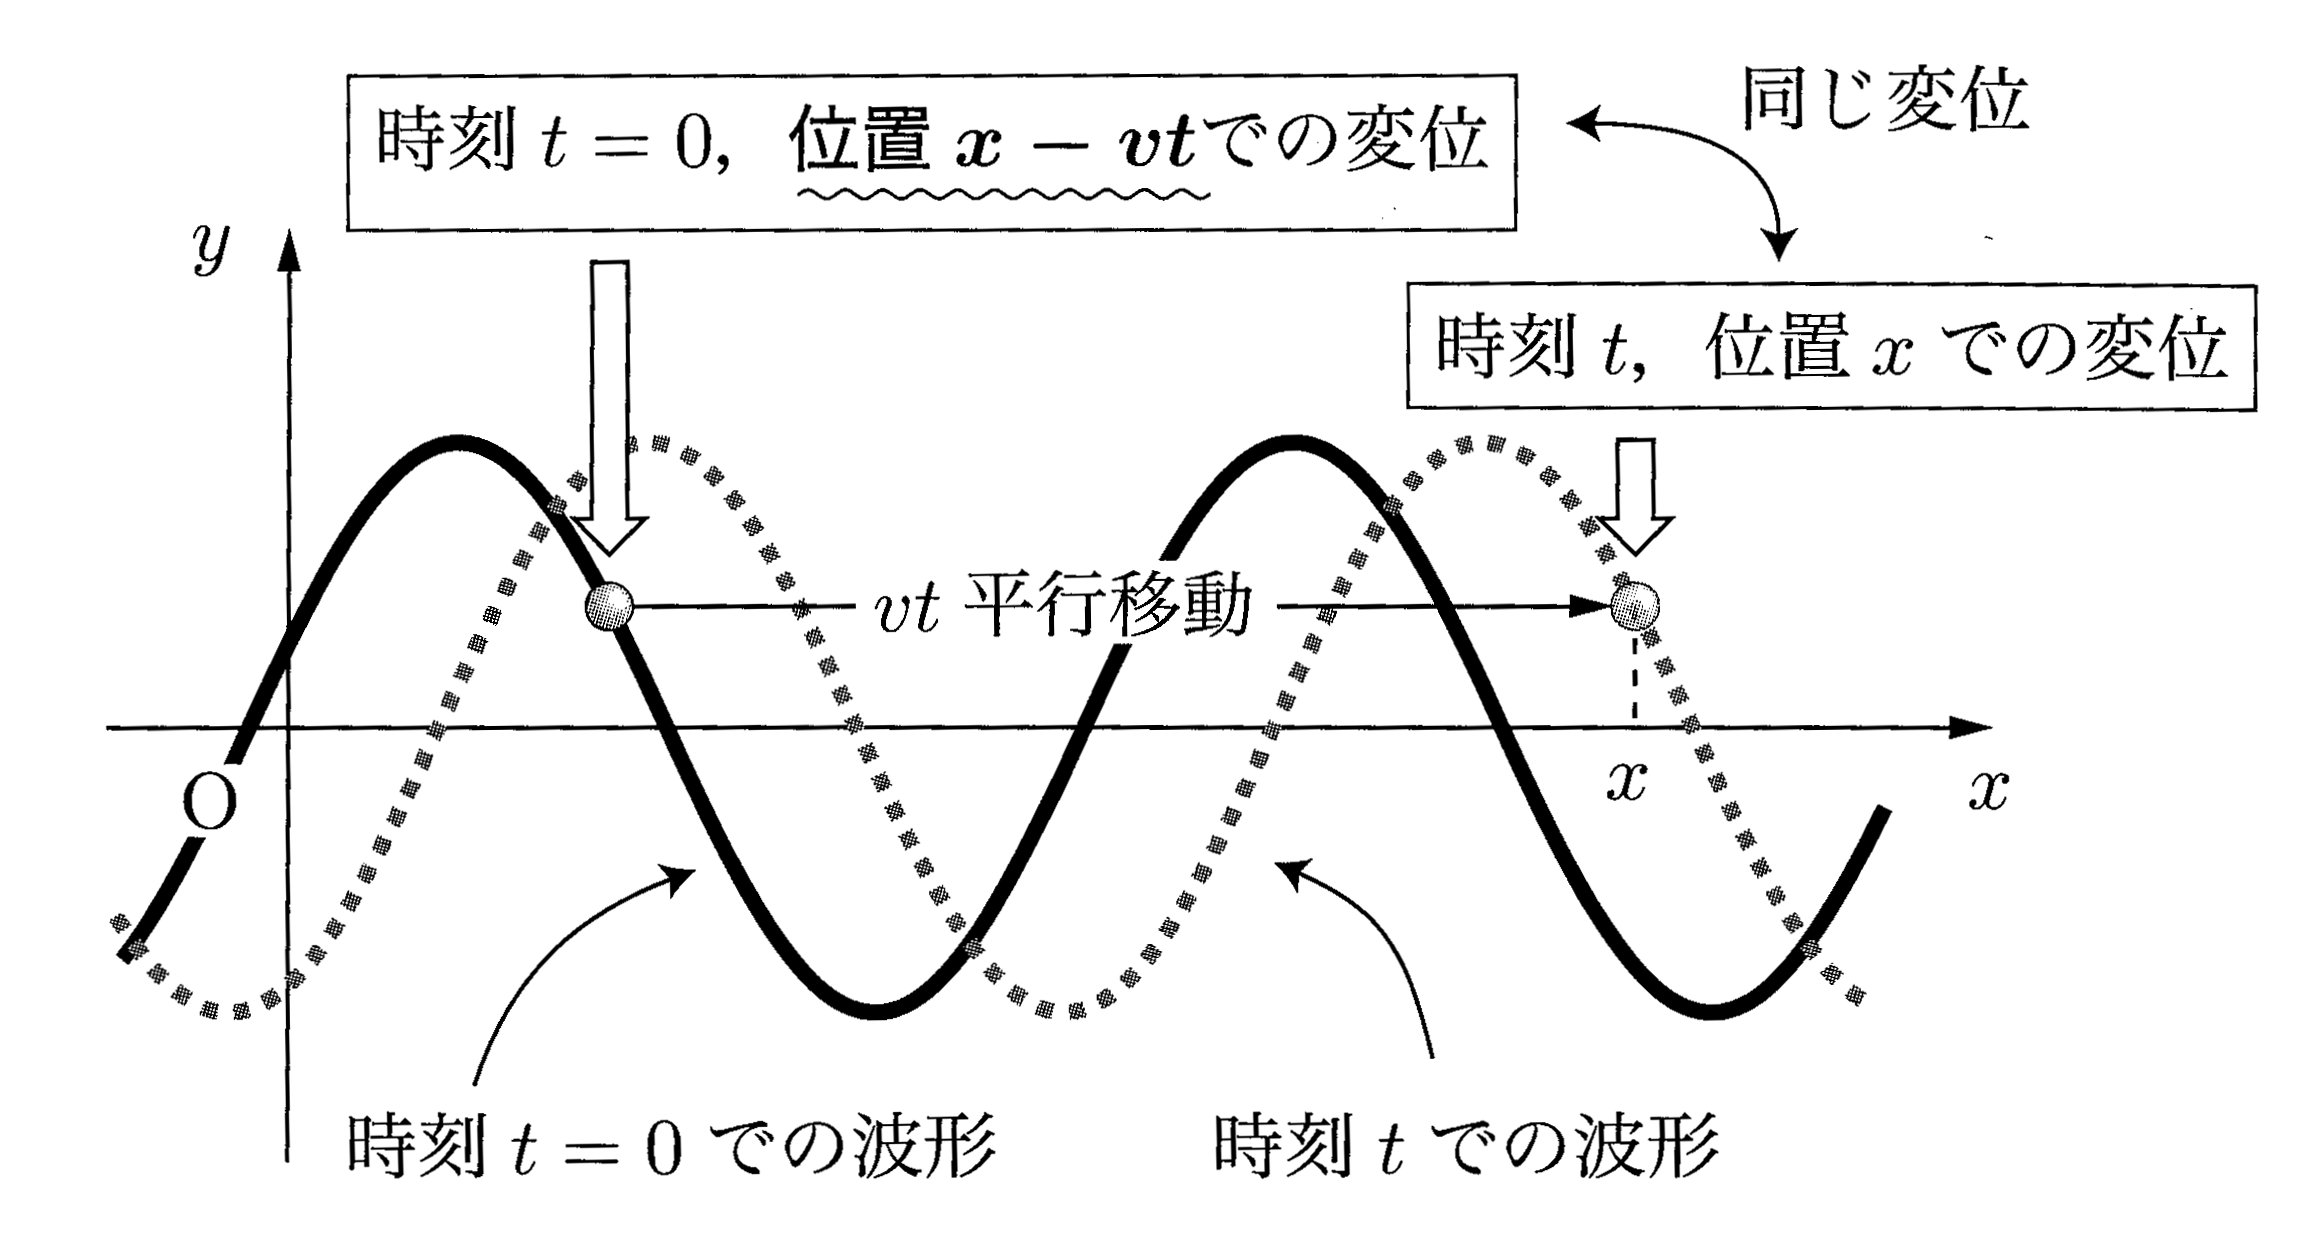
\includegraphics[keepaspectratio,width=100mm]
  {text_p87_fig1.png}
\end{wrapfigure}
この波が右方向に速さ$v$[m/s]で進んでいる場合について，任意の$t$[s]に対する変位$y(x,t)$を得ることを考えてみる．
時刻$t$[s]に位置$x$[m]にいる波は，時刻$t=0$[s]には距離$vt$[m]だけ手前の位置，すなわち$x-vt$[m]の場所にあったはずである．
よって，{\bf 時刻} \mbox{\boldmath $t$} {\bf [s]の位置} \mbox{\boldmath $x$} {\bf [m]の変位は，時刻} \mbox{\boldmath $t=0$} {\bf [s]の位置} \mbox{\boldmath $x-vt$} {\bf [m]の変位と一致していなければならない}から，
\[ \mbox{\boldmath $y(x,t)=y(x-vt,0)$}\]
が成立する．
すなわち，先ほど表した$y(x,0)$の式の$x$を$x-vt$に取り替えればよい．

利用できる波形のグラフが時刻$t=0$[s]のものでない場合や，波が左方向に進んでいる場合などはどのように置き換えるかはその都度考える必要があるが，その基本は，
\begin{matome}{波形グラフからの正弦波の一般表式の導出}
 \hspace{3mm} $\MARU{1} \hspace{2mm} 与えられたある時刻の波形グラフを数式で表す．（通常はt=0[{\rm s}]で考える）$\\
  \hspace{3mm} $\MARU{2} \hspace{2mm} 一般の時刻t[{\rm s}]における変位は，\MARU{1} の時刻ではどの位置にあったものかを計算する．$\\
   \hspace{3mm} $\MARU{3} \hspace{2mm} \MARU{2} を元に，y(x,t)を\MARU{1} の式から導く．右方向へ進むならy(x,t)=y(x-vt,0)$
 \end{matome}
である．


\subsection{$y-x$グラフと$y-t$グラフ}
波動の方程式は$x,t$の2変数関数であるから，ある波動の変位をグラフで表そうとした場合，どちらの変位を固定してグラフにするかでその方法は2通りある．
\begin{matome}{波動のグラフ化}
 \hspace{3mm} $・y-xグラフ$\\
  \hspace{5mm} ある瞬間における波の波形を，横軸に位置$x$[m]，縦軸に変位$y$[m]をとって表したグラフ\\
 \hspace{3mm} $・y-tグラフ$\\
  \hspace{5mm} ある1点の上下振動を，横軸に時間$t$[s]，縦軸に変位$y$[m]をとって表したグラフ
 \end{matome}

いずれのグラフでも$\sin$カーブが現れるが，それらが意味するところは全く異なることに注意せよ．
またこれらのグラフは相互変換することができる．

\subsection{$y-t$グラフによる正弦波の一般式の導出}
ある瞬間における波形$y-x$グラフから正弦波の一般式を導出する方法を前々節で学んだが，問題文で与えられる波のグラフが，ある1点（通常は原点）の上下振動を$y-t$グラフとして表したものであることもしばしばある．
ここでは，与えられた$y-t$グラフから任意の時刻，位置における変位$y(x,t)$[m]を求める方法を学ぶ．
与えられた$y-t$グラフが原点$x=0$[m]における振動を表した$y-t$であり，波が右方向に速さ$v$[m/s]で進んでいる場合を考えよう．
まず，与えられた$y-t$グラフを具体的数式で表せば，$y(0,t)$[m]が得られる．

\begin{wrapfigure}[12]{r}[5mm]{100mm}
  \centering
  \vspace{-5mm}
  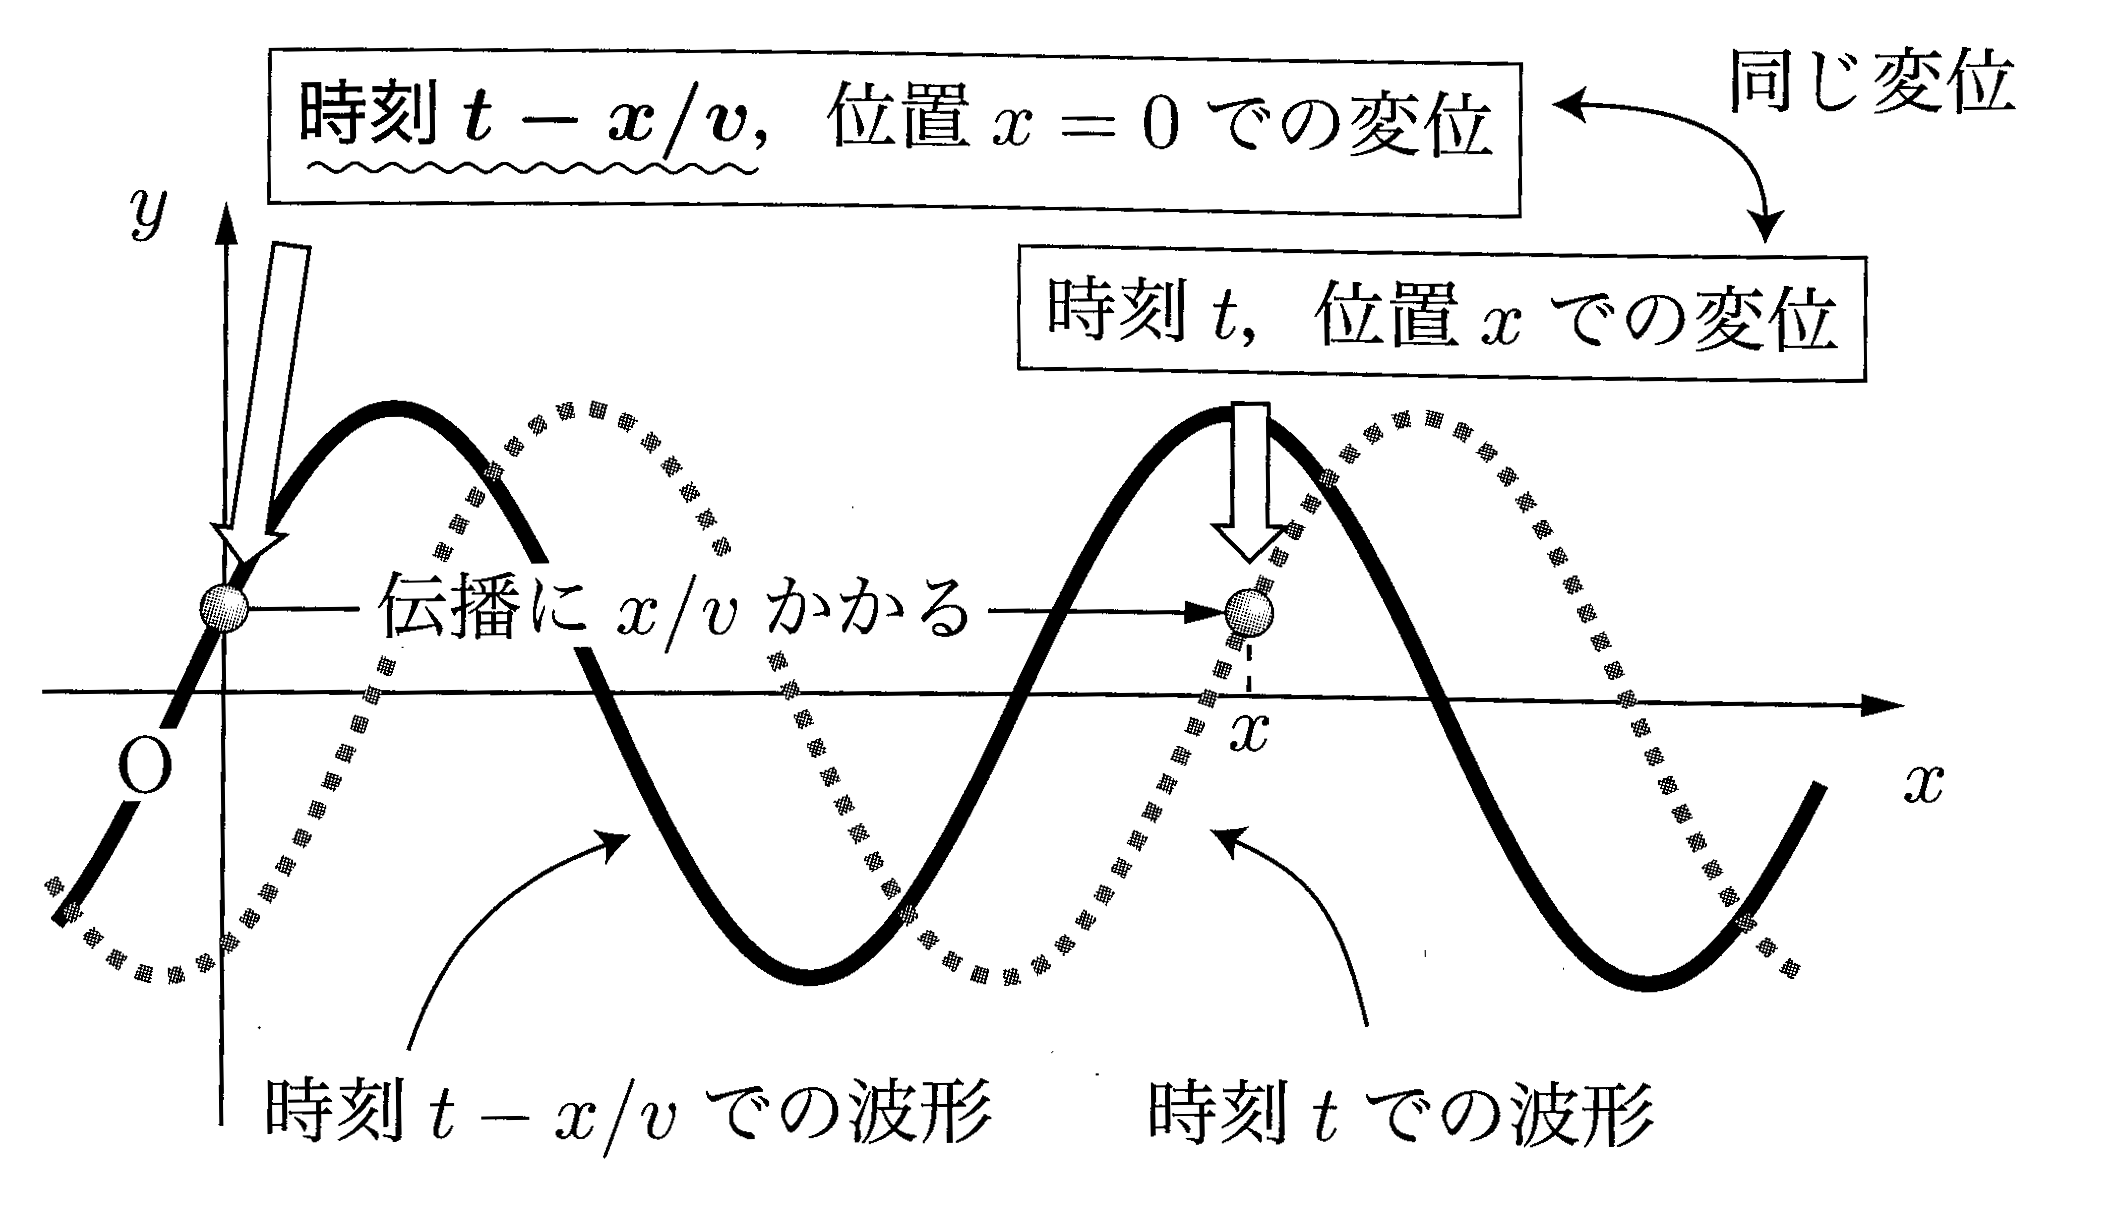
\includegraphics[keepaspectratio,width=100mm]
  {text_p89_fig1.png}
\end{wrapfigure}
これを元に任意の$t$[s]に対する変位$y(x,t)$[m]を得るためには，時刻$t$[s]に位置$x$[m]にいる波が，原点をいつ通過したかを考えればよい．
位置$x$[m]に来るためには原点から$\dfrac{x}{v}$[s]だけかかるから，時刻$t$[s]に位置$x$[m]にある波は原点を$t-\dfrac{x}{v}$[s]に通過した波である．
よって，{\bf 時刻} \mbox{\boldmath $t$} {\bf [s]における位置} \mbox{\boldmath $x$} {\bf [m]の変位は，原点における時刻} \mbox{\boldmath $t-\dfrac{x}{v}$} {\bf [s]の変位と一致していなければならない}ので，
\[\mbox{\boldmath $y(x,t)=y\left( 0,t-\dfrac{x}{v}\right)$}\]
が成立する．
すなわち，先ほど表した$y(0,t)$の式の$t$を，$t-\dfrac{x}{v}$に取り替えれば$y(x,t)$が得られる．

利用できる$y-t$グラフが原点のものでない場合や，波が左方向に進んでいる場合などはどのように置き換えるかをその都度考える必要があるが，その基本は次の通りである．

\begin{matome}{振動グラフからの正弦波の一般表式の導出}
 \hspace{3mm} $\MARU{1} \hspace{2mm} 与えられたある点の振動グラフを数式で表す．（通常はx=0[{\rm m}]で考える）$\\
  \hspace{3mm} $\MARU{2} \hspace{2mm} 一般のx[{\rm m}]における変位は，\MARU{1} の点をどの時刻に通過したものかを計算する．$\\
   \hspace{3mm} $\MARU{3} \hspace{2mm} \MARU{2} を元に，y(x,t)を\MARU{1} の式から導く．右方向へ進むならy(x,t)=y\left(0,t-\dfrac{x}{v}\right)$
 \end{matome}

\subsection{正弦波の一般式の一般形}
以上で求めてきた正弦波の任意の時刻，任意の位置の変位$y(x,t)$[m]は必ず
\[ y(x,t)=A\sin \left\{ 2\pi \left( \dfrac{t}{T}\pm \dfrac{x}{\lambda} \right) +\varphi_0 \right\}  \hspace{5mm} (A,\varphi_0 は定数) \]
の形にまとめることができる．
この式を覚えておく必要はないが，正弦波がグラフではなく数式で与えられた場合はこの三角関数の中身の部分に着目して考えるとよい．

三角関数の角度部分を{\bf 位相}と呼ぶ．
\[\varphi (x,t)=2\pi \left( \dfrac{t}{T}\pm \dfrac{x}{\lambda} \right) +\varphi_0\]

この位相が同じ値であれば変位$y(x,t)$は同じになる．
ゆえに，波が進行していくということは同一位相の点が右もしくは左へずれていくということを意味する．
これより，位相部分の$x,t$の係数が{\bf 異符号であれば波は右方向へ，同符号であれば波は左方向へ進行する}ということが言える．

また，位相は$2\pi$ずれても同じ変位になることに注意すると，ある時刻$t$[s]において位置$x$[m]が$\lambda$[m]だけずれると位相が$2\pi$だけずれるので同一変位となる．
よって，同一時刻において位置のずれを位相のずれに換算するなら，{\bf 1波長のずれが位相} \mbox{\boldmath $2\pi$} {\bf のずれに対応する．}

またある位置において時刻$t$[s]が変化していくと，時刻が$T$[s]だけずれると位相が$2\pi$だけずれて再び同一変位となる．よって，ある位置において時刻のずれを位相のずれに換算するなら，{\bf 1周期}\mbox{\boldmath $T$}{\bf [s]のずれが位相} \mbox{\boldmath $2\pi$}{\bf のずれに対応する．}

また，{\bf 位相が}\mbox{\boldmath $\pi$}{\bf ずれているとその変位がちょうど正負逆}となる．
このような2つの位相を{\bf 互いに逆位相である}という．
\begin{matome}{正弦波のまとめ}
 \hspace{3mm} $・三角関数の角度の部分を位相と呼ぶ．この位相が2\pi ずれても同じ変位になる．$\\
 \hspace{3mm} $・位相部分のx，tが異符号なら右方向へ，同符号なら左方向へ進行する波である．$\\
 \hspace{3mm} $・ある時刻において，位置が\lambda [{\rm m}]ずれると位相は2\pi ずれる．$\\ 
 \hspace{3mm} $・ある位置において，時刻がT[{\rm s}]ずれると位相は2\pi ずれる．$\\ 
 \hspace{3mm} $・位相が\pi ずれると変位は上下逆となる．$\end{matome}


\newpage

\begin{figure}[h]
\begin{center}
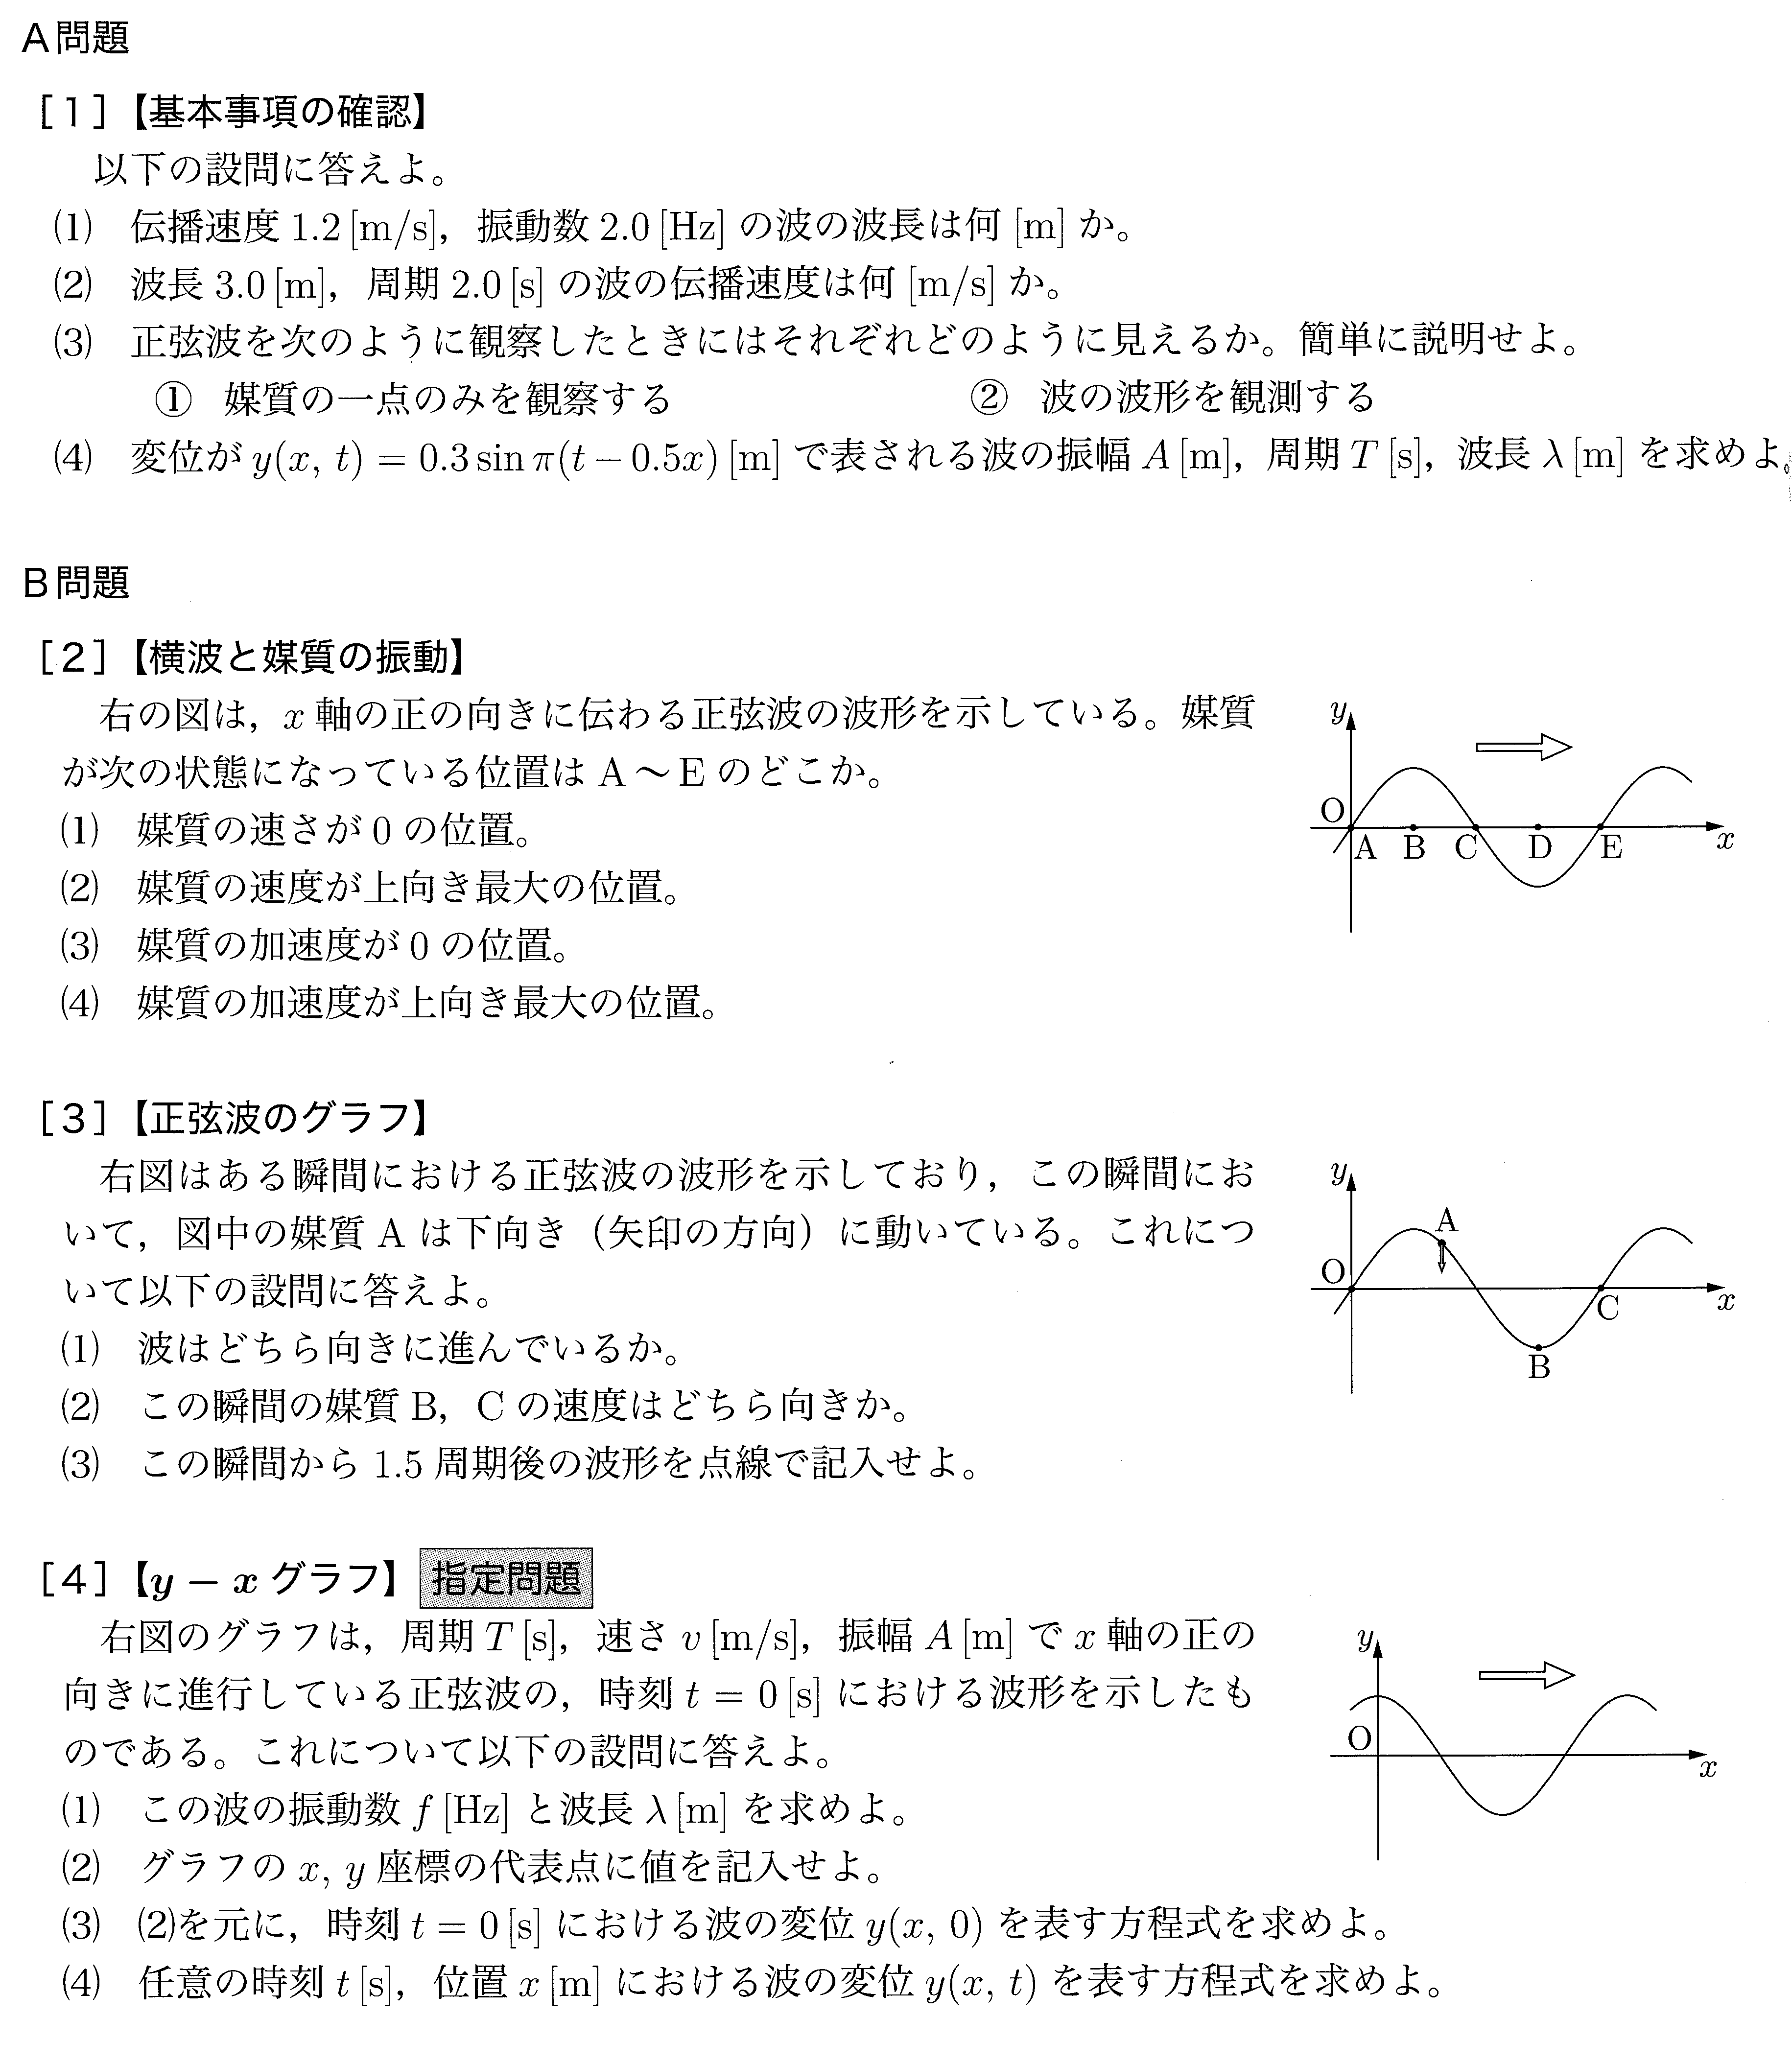
\includegraphics[width=170mm]{prob_p48.png}
\end{center}
\end{figure}

\newpage

\begin{figure}[h]
\begin{center}
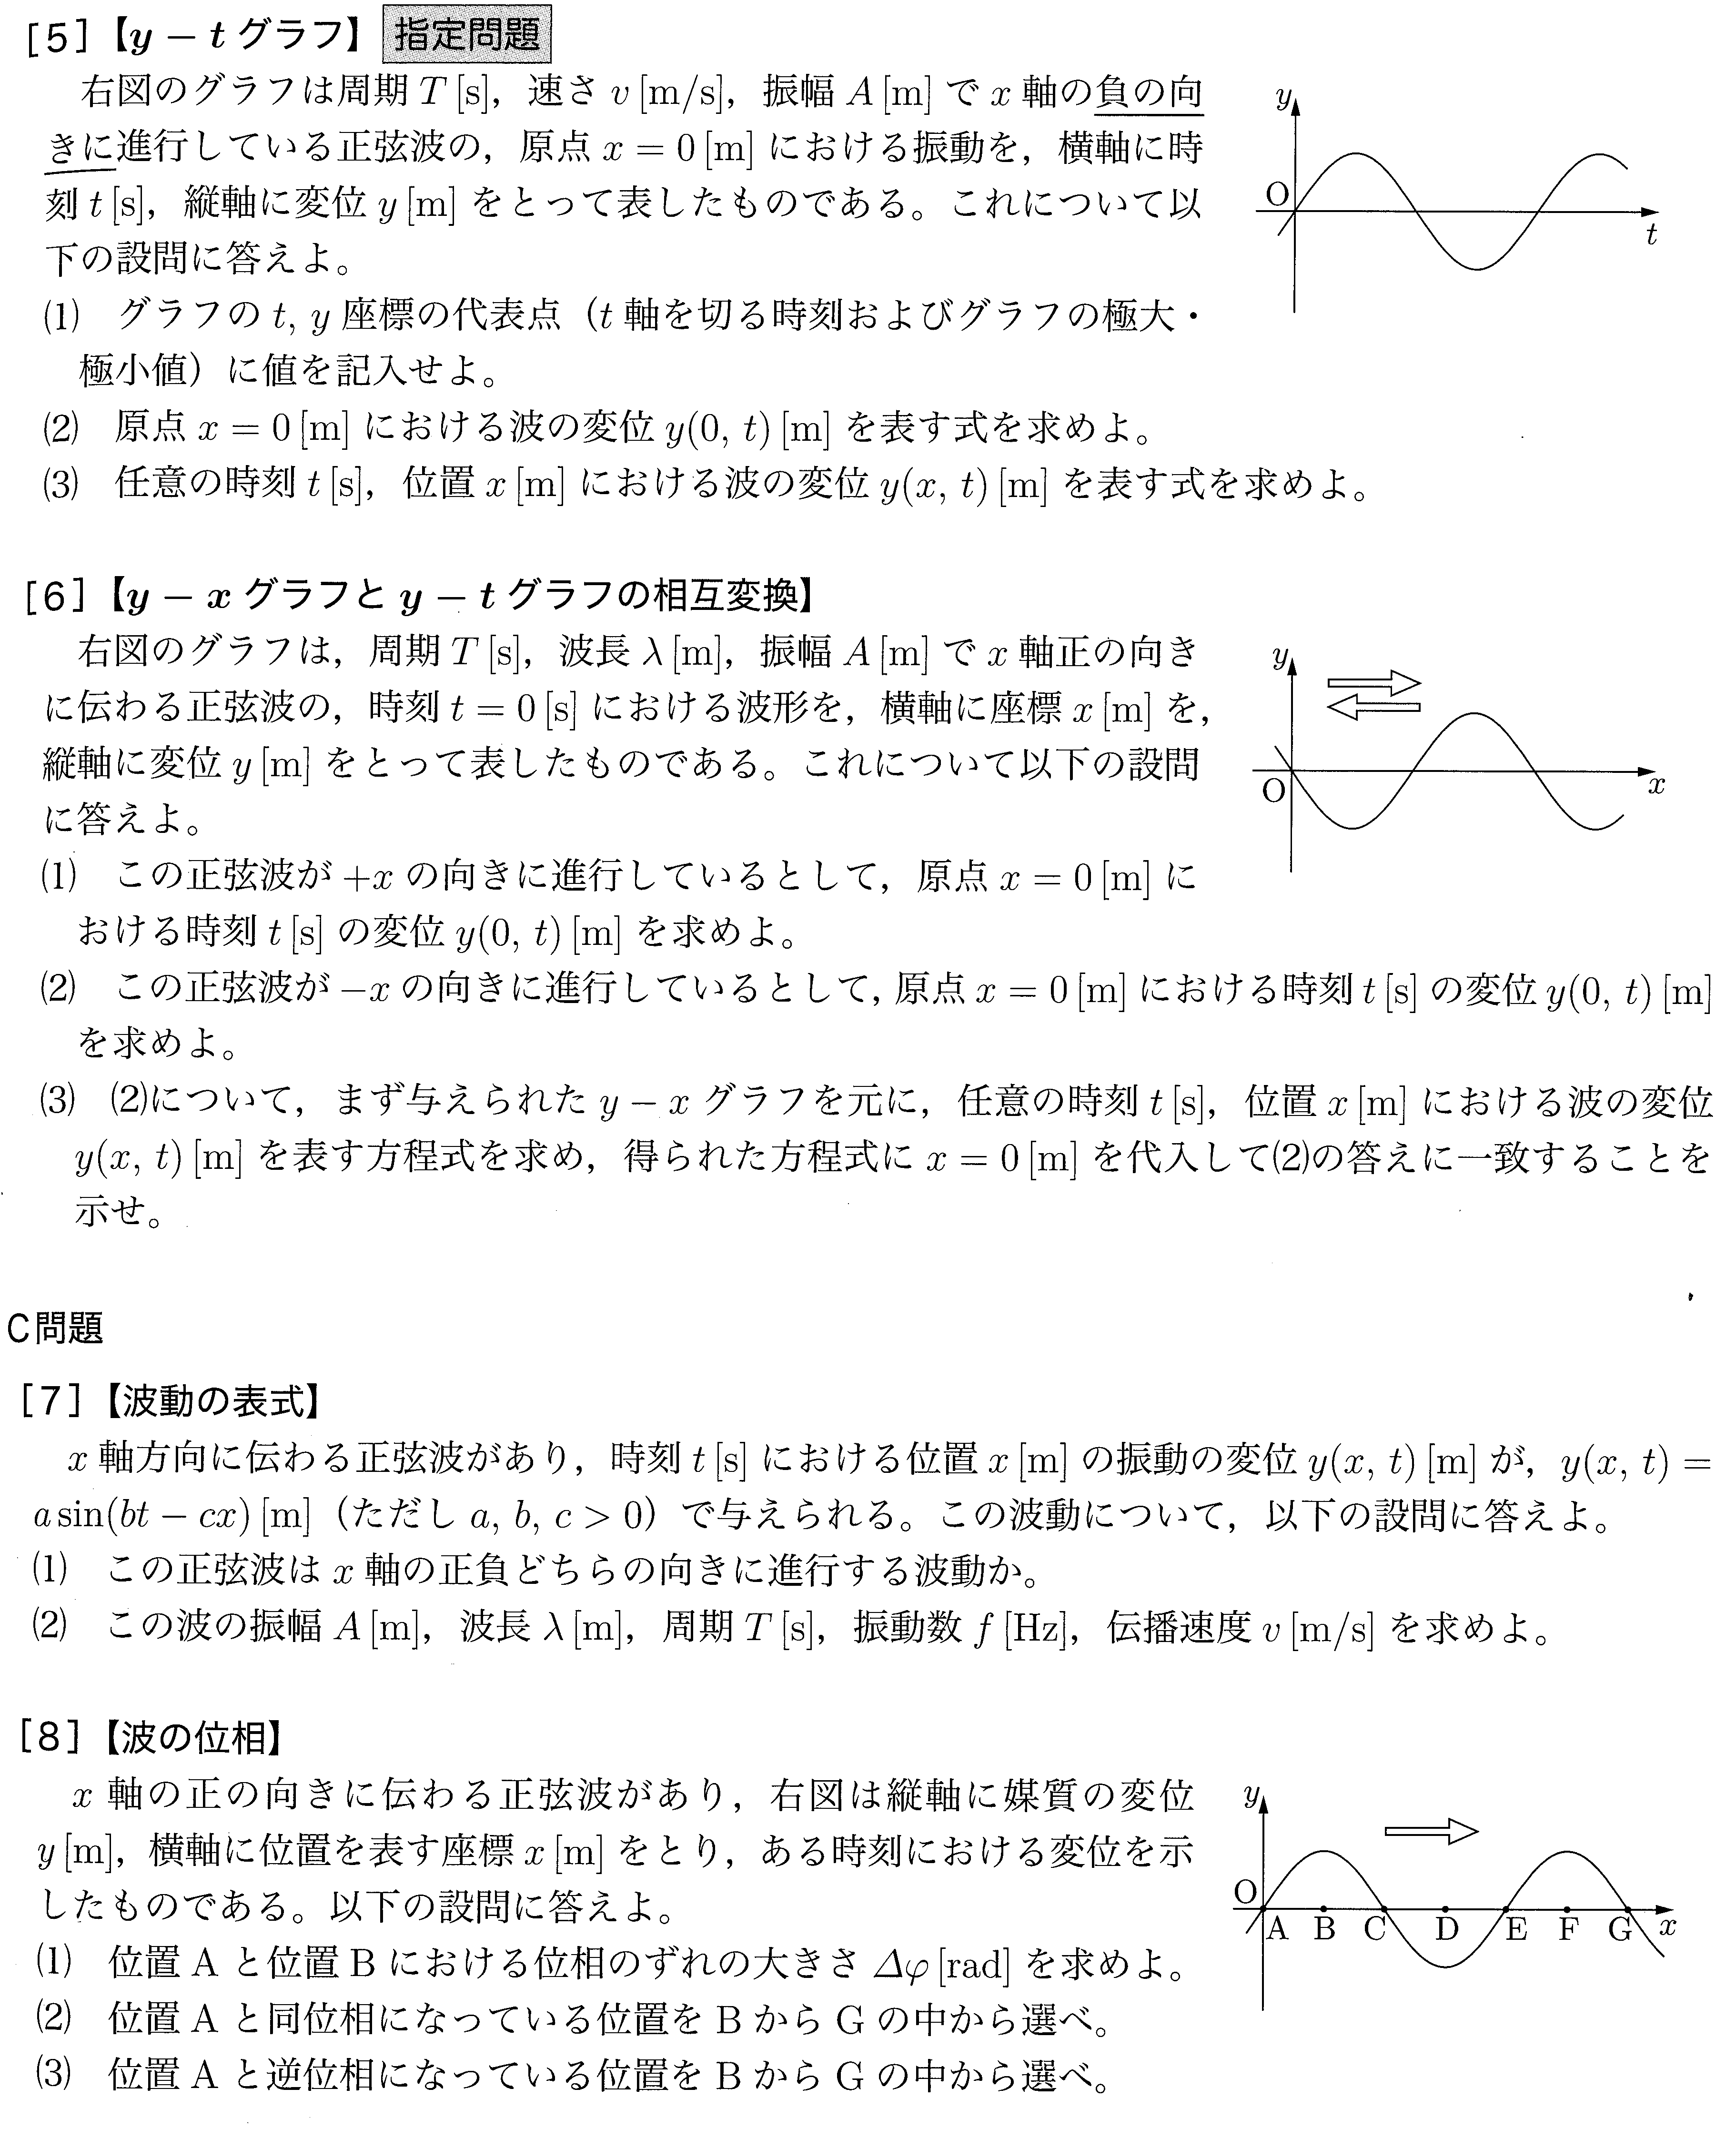
\includegraphics[width=170mm]{prob_p49.png}
\end{center}
\end{figure}


\newpage

\begin{figure}[h]
\begin{center}
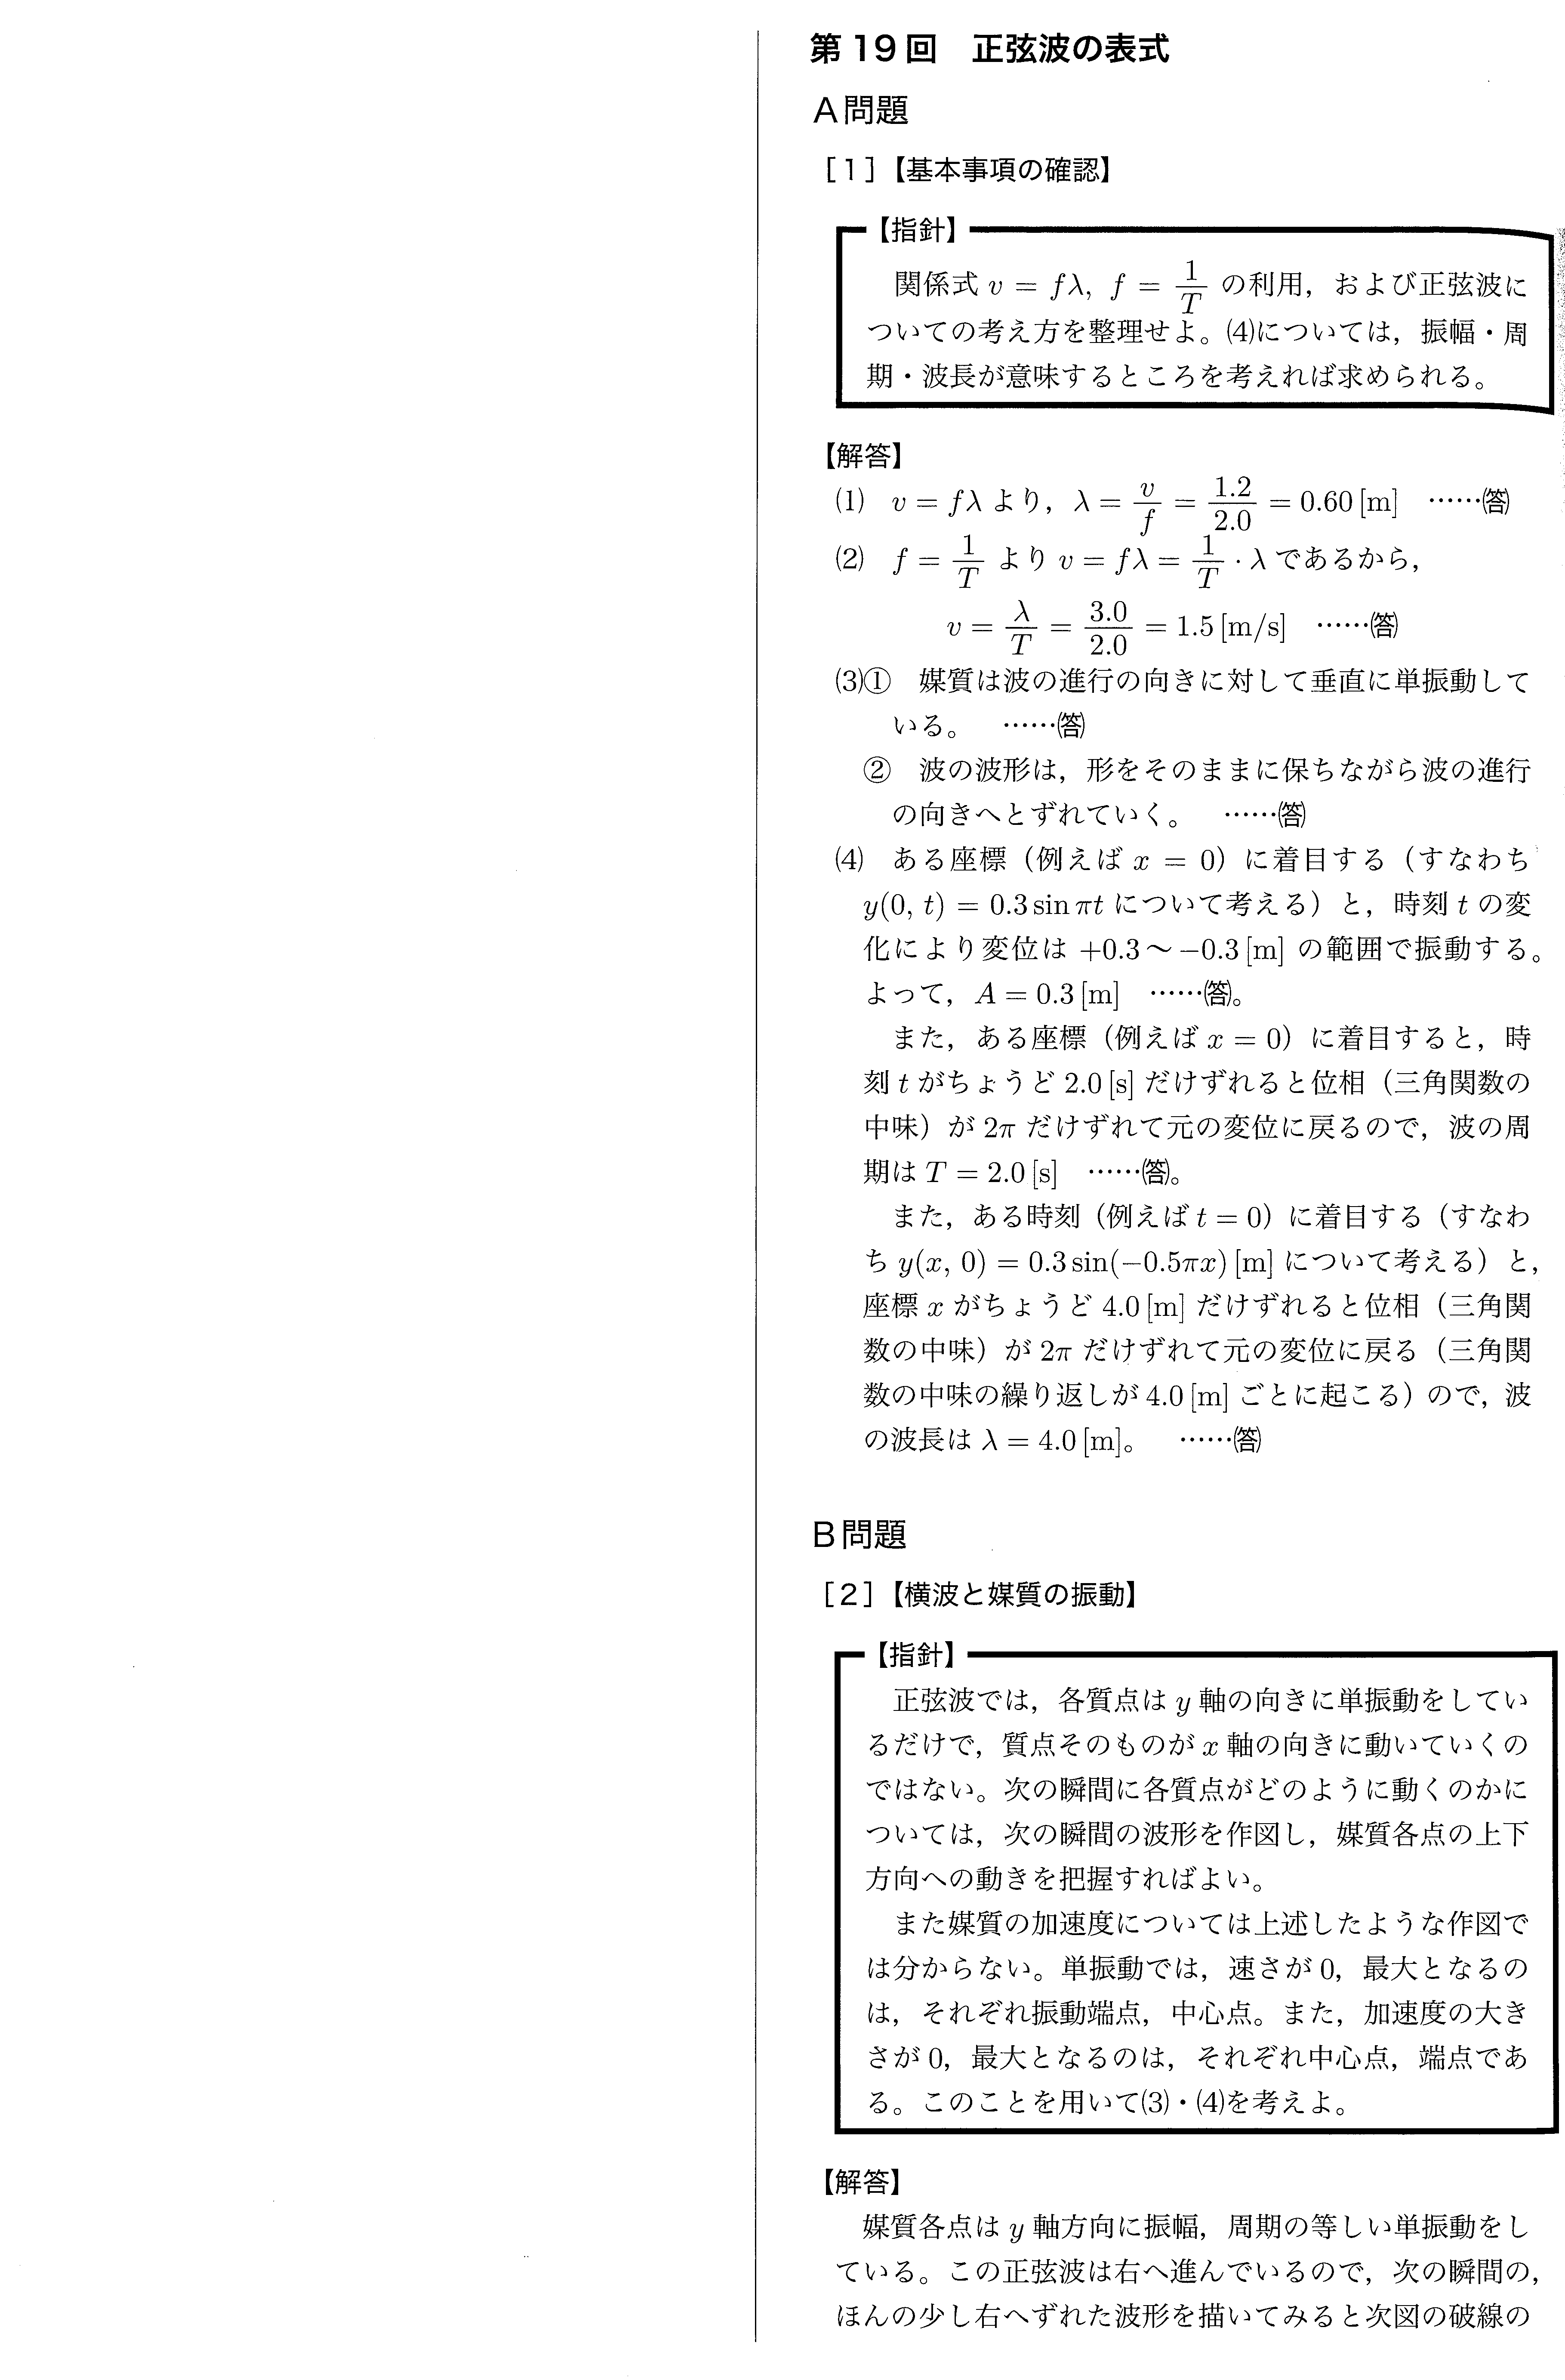
\includegraphics[width=170mm]{prob_p142_2.png}
\end{center}
\end{figure}

\newpage

\begin{figure}[h]
\begin{center}
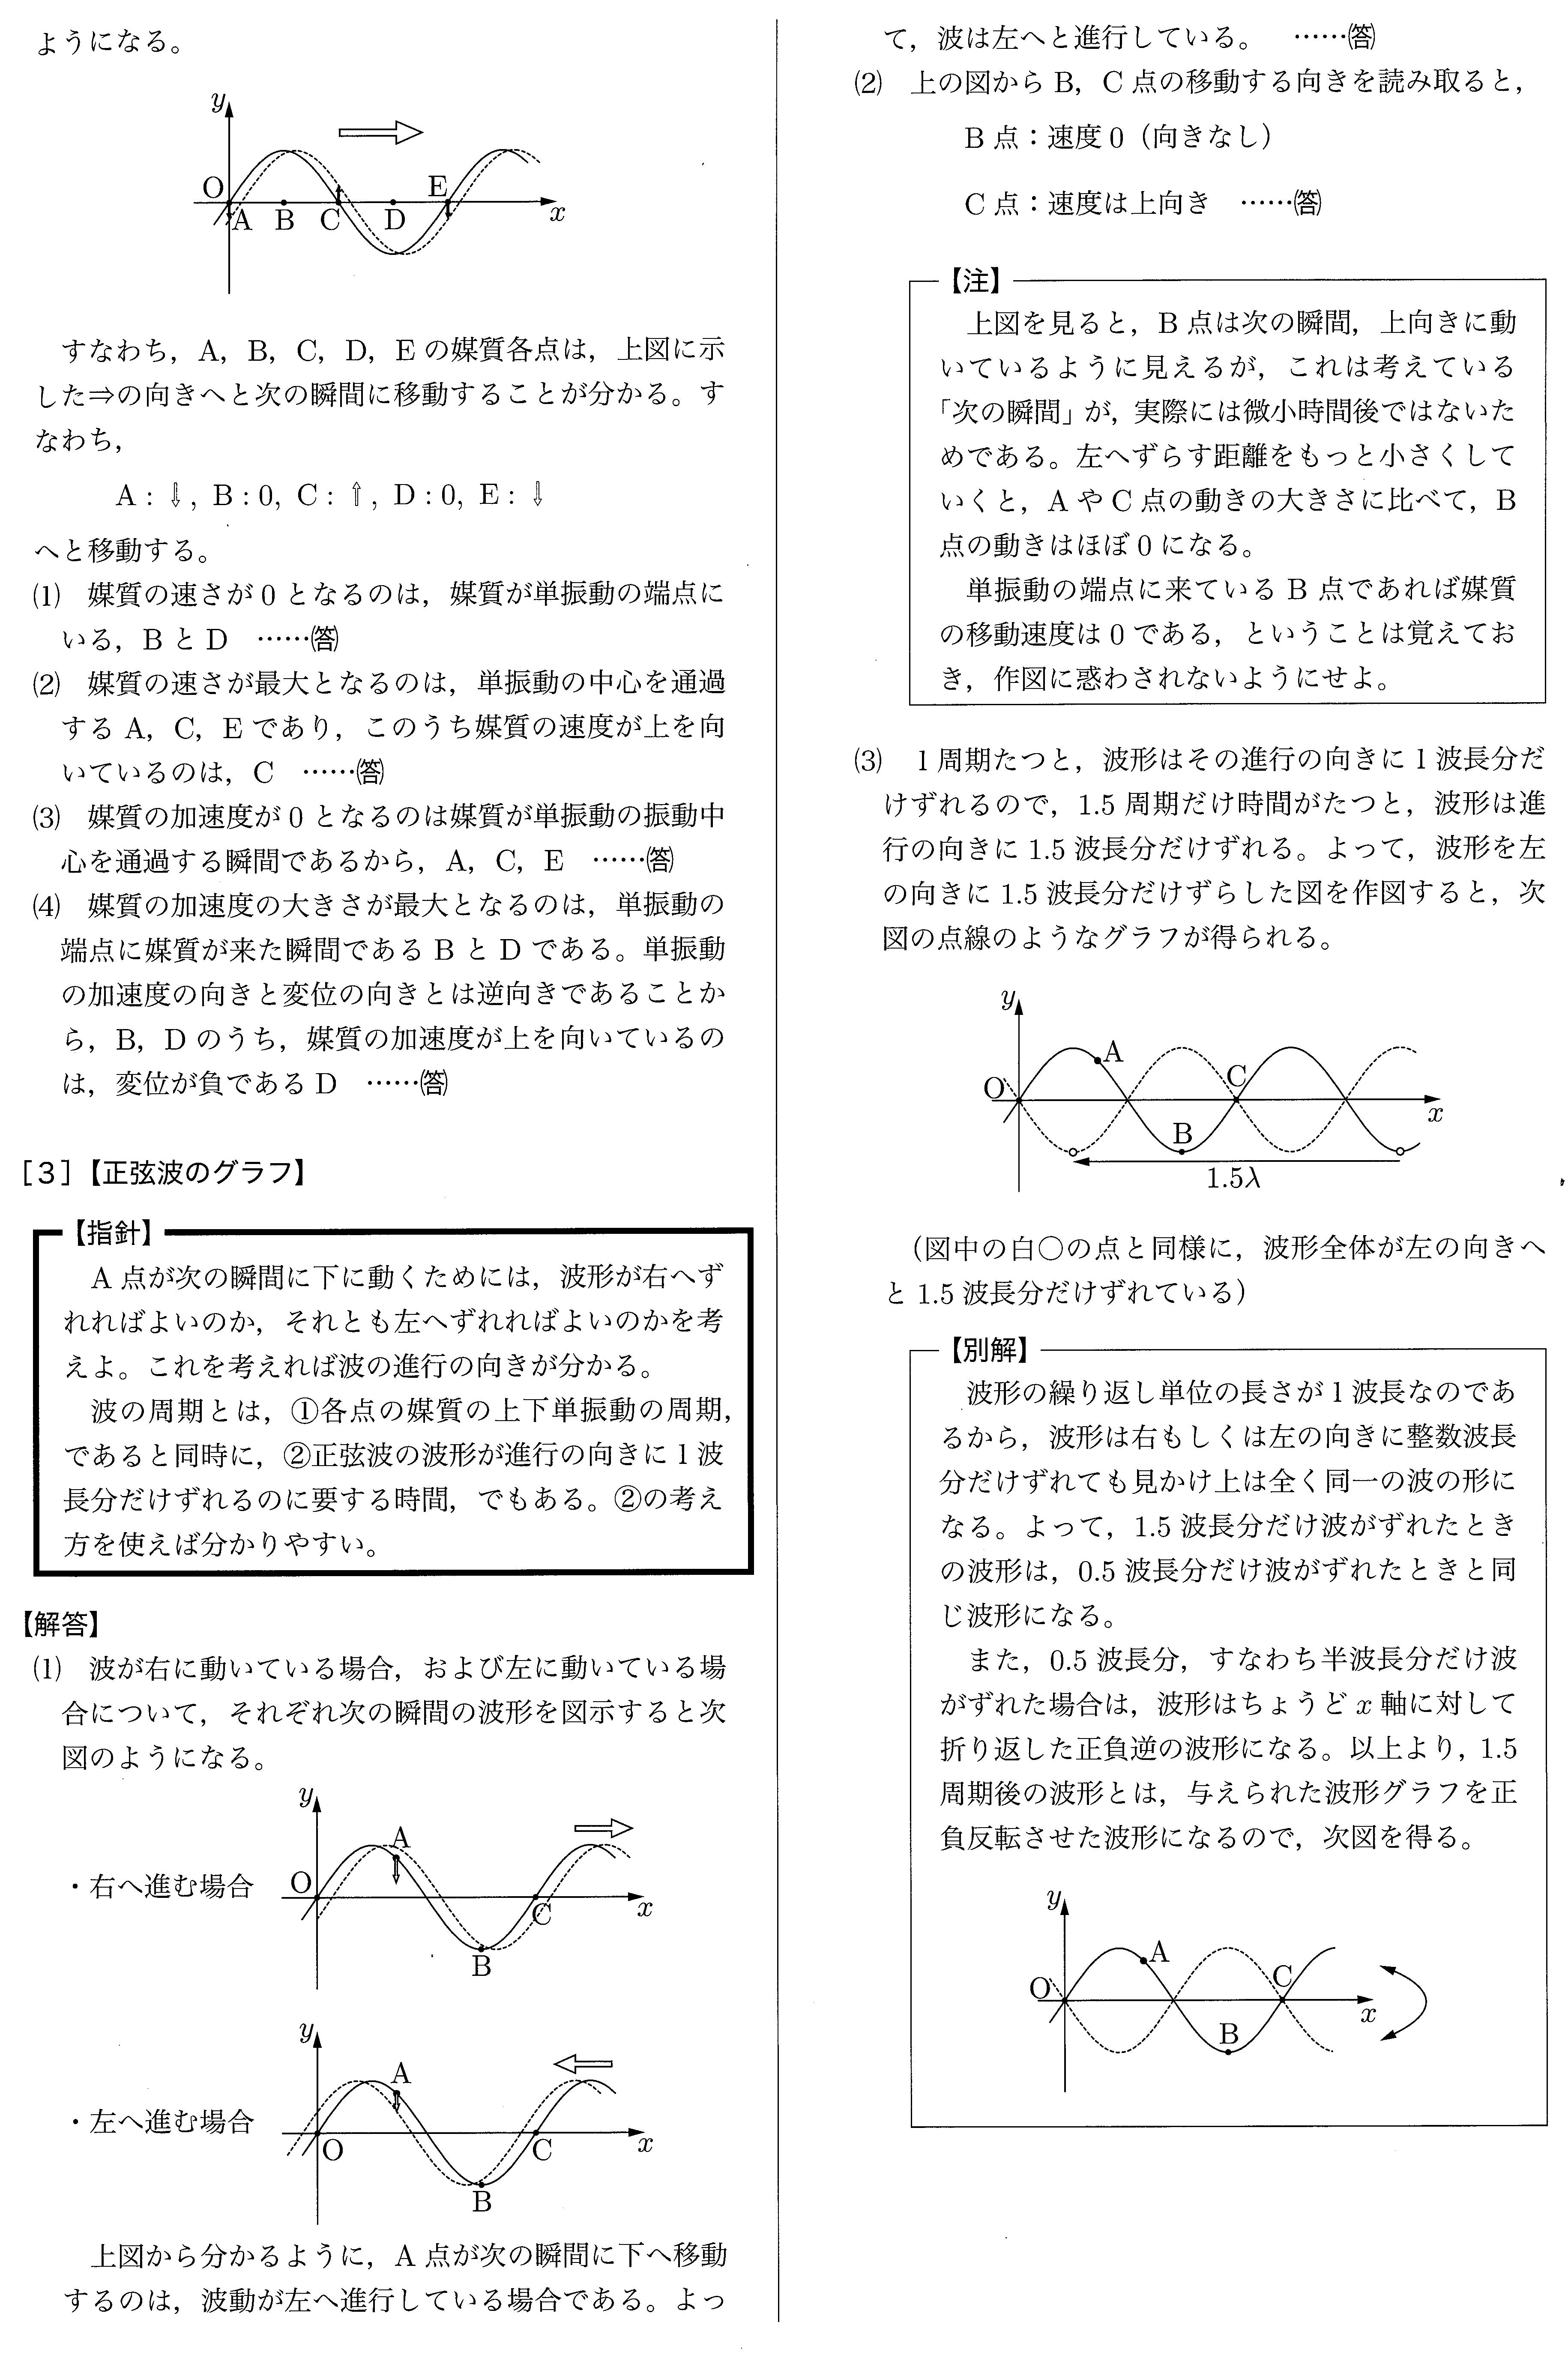
\includegraphics[width=170mm]{prob_p143.png}
\end{center}
\end{figure}

\newpage

\begin{figure}[h]
\begin{center}
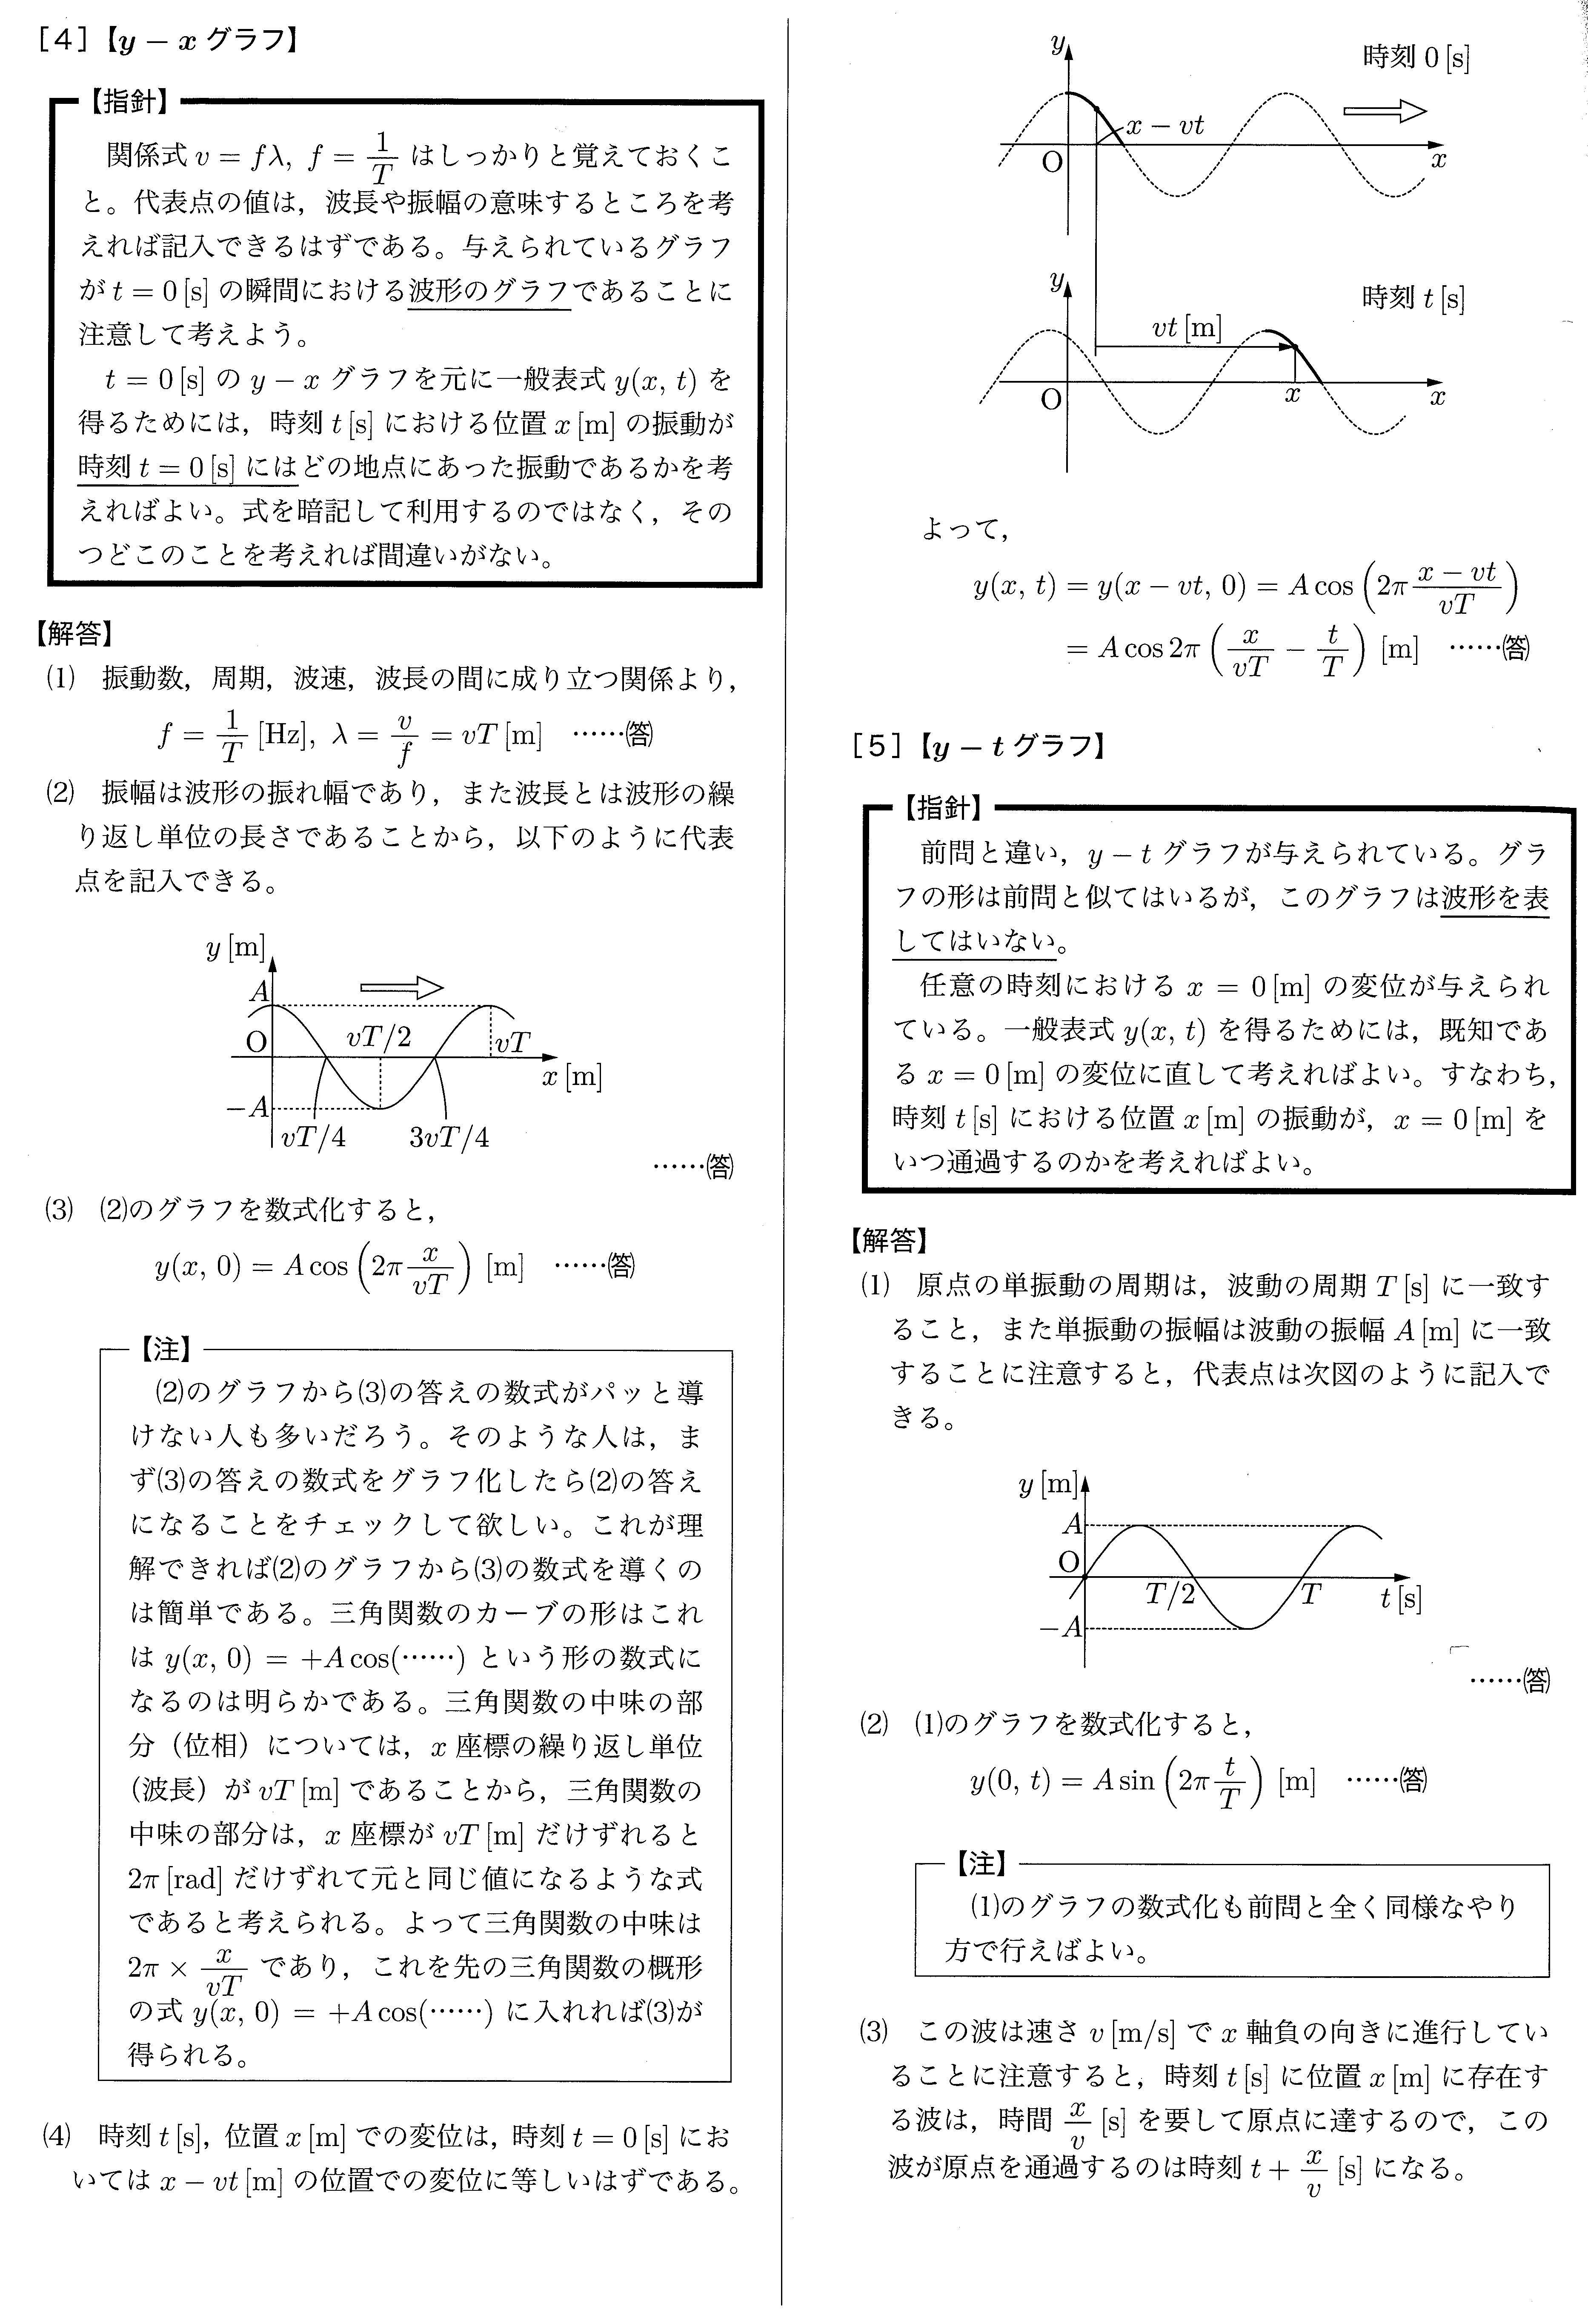
\includegraphics[width=170mm]{prob_p144.png}
\end{center}
\end{figure}

\newpage

\begin{figure}[h]
\begin{center}
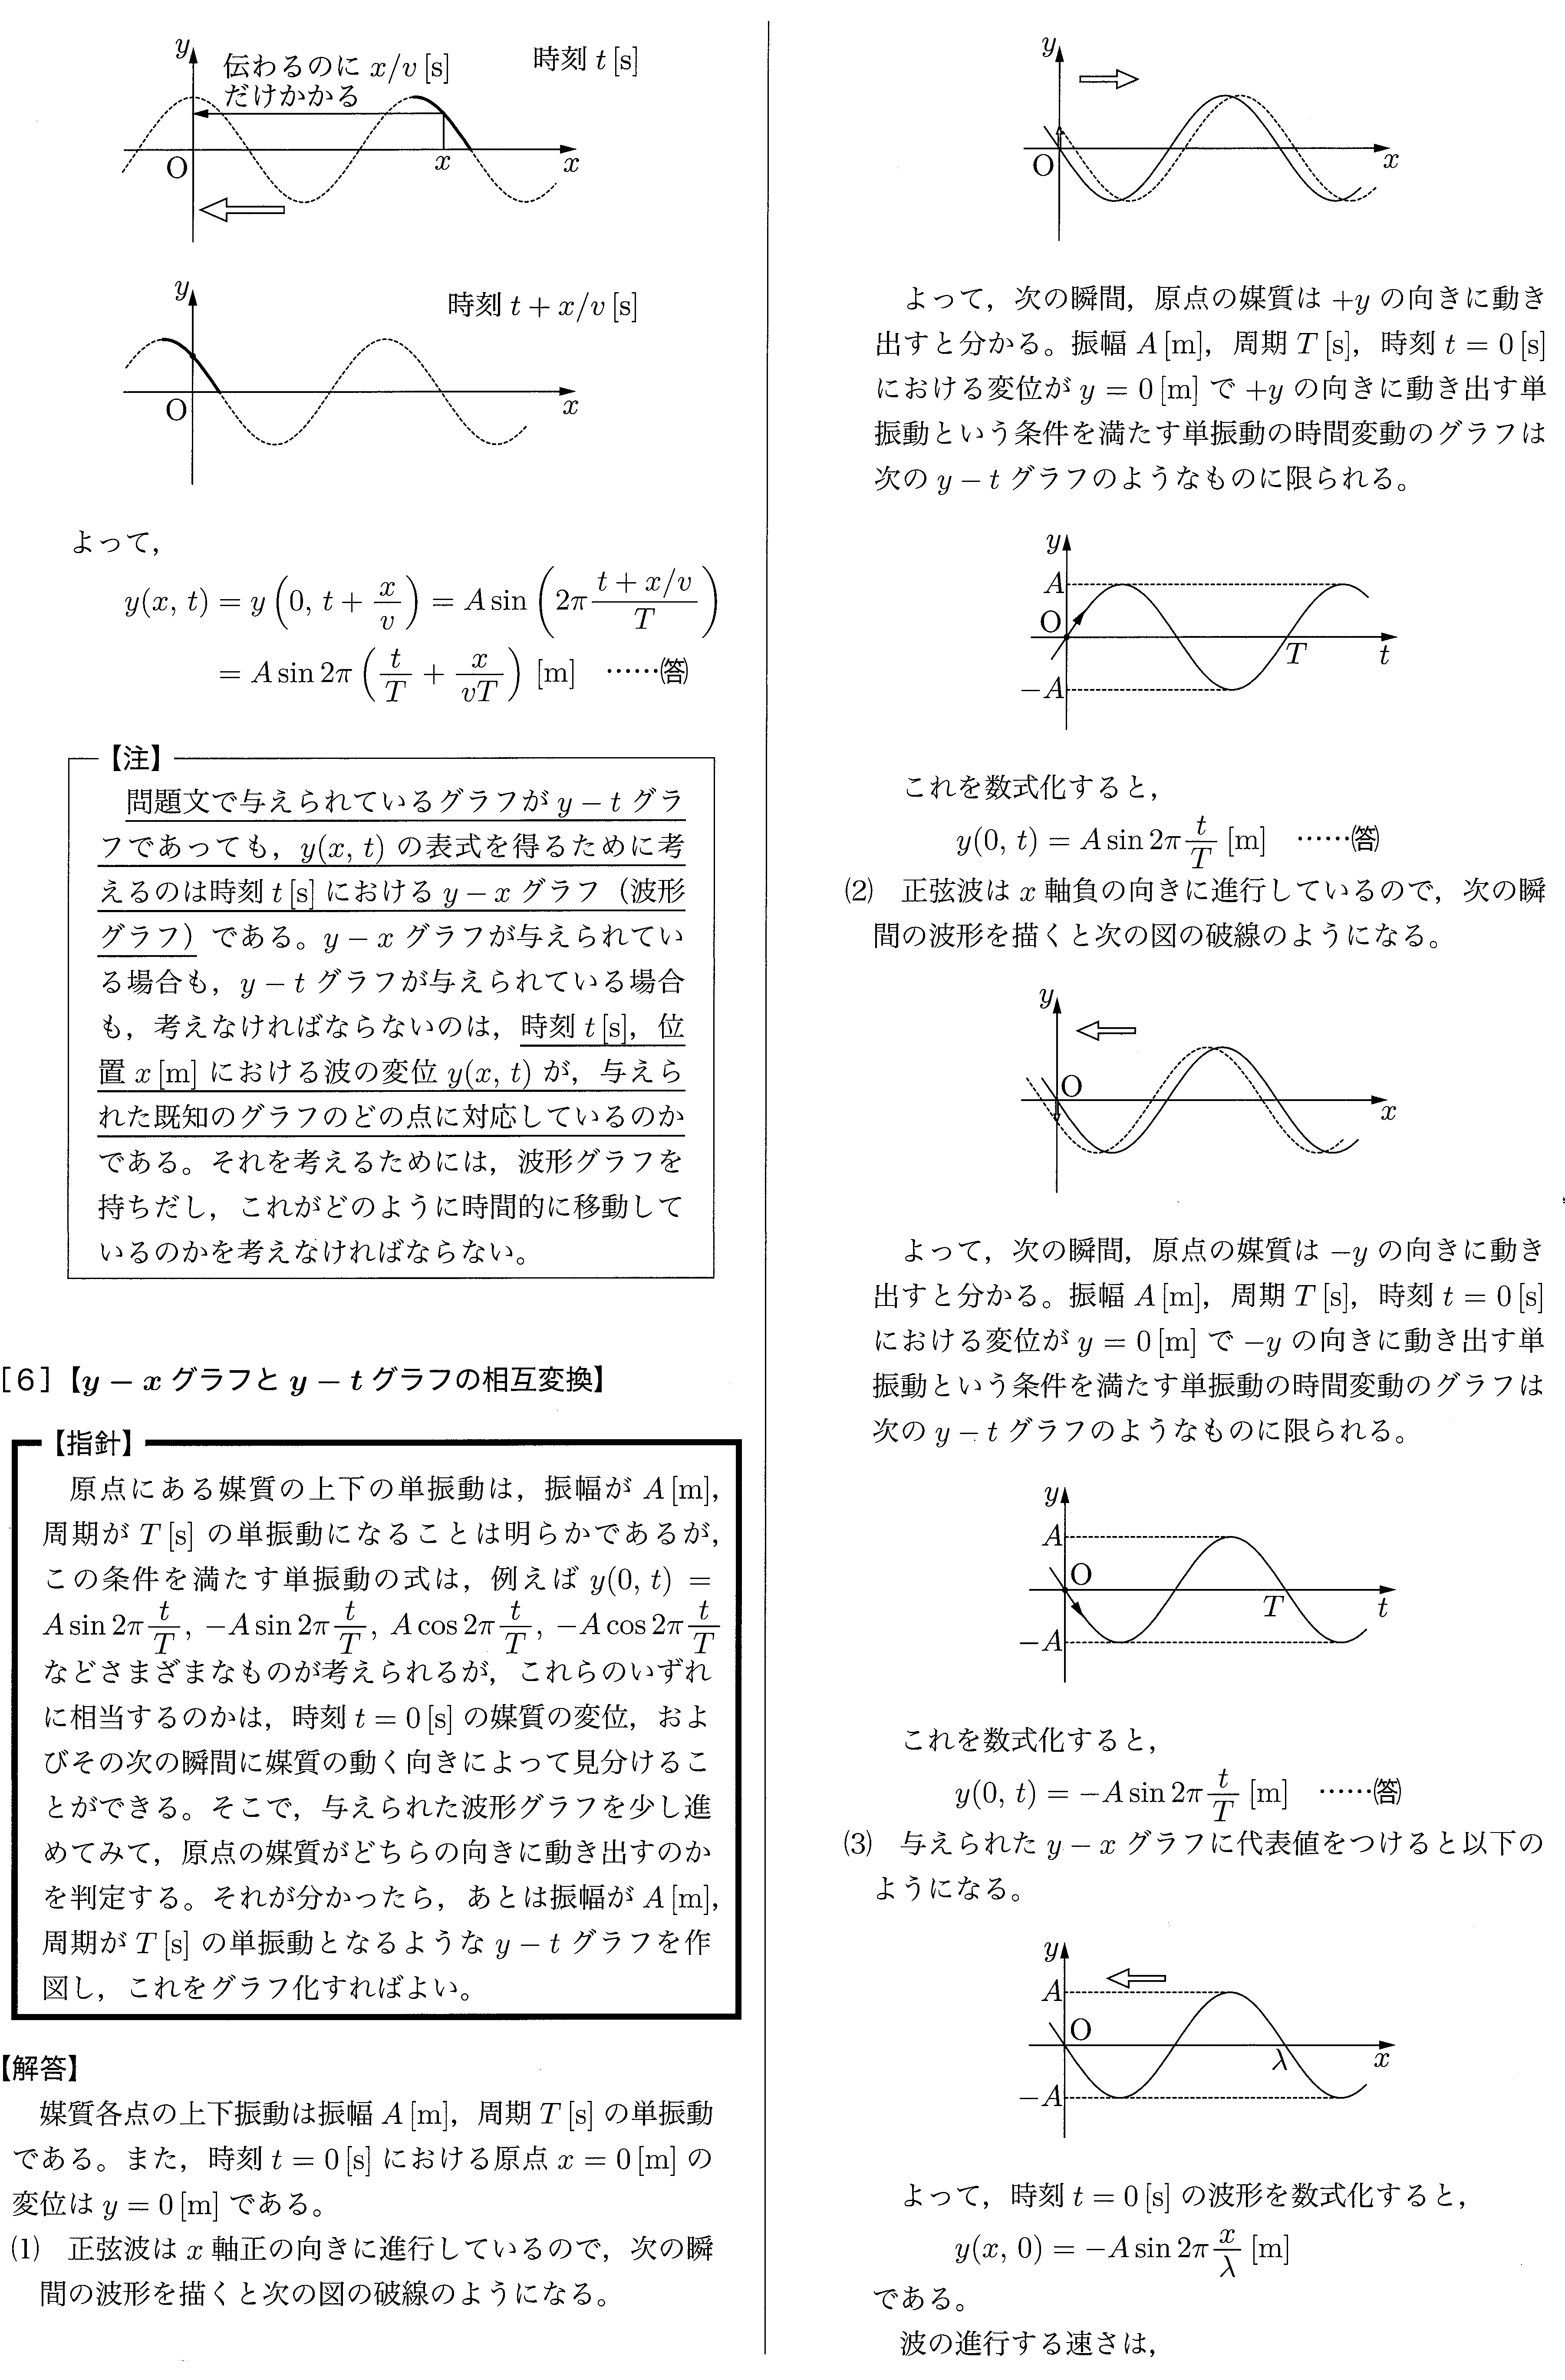
\includegraphics[width=170mm]{prob_p145.png}
\end{center}
\end{figure}

\newpage

\begin{figure}[h]
\begin{center}
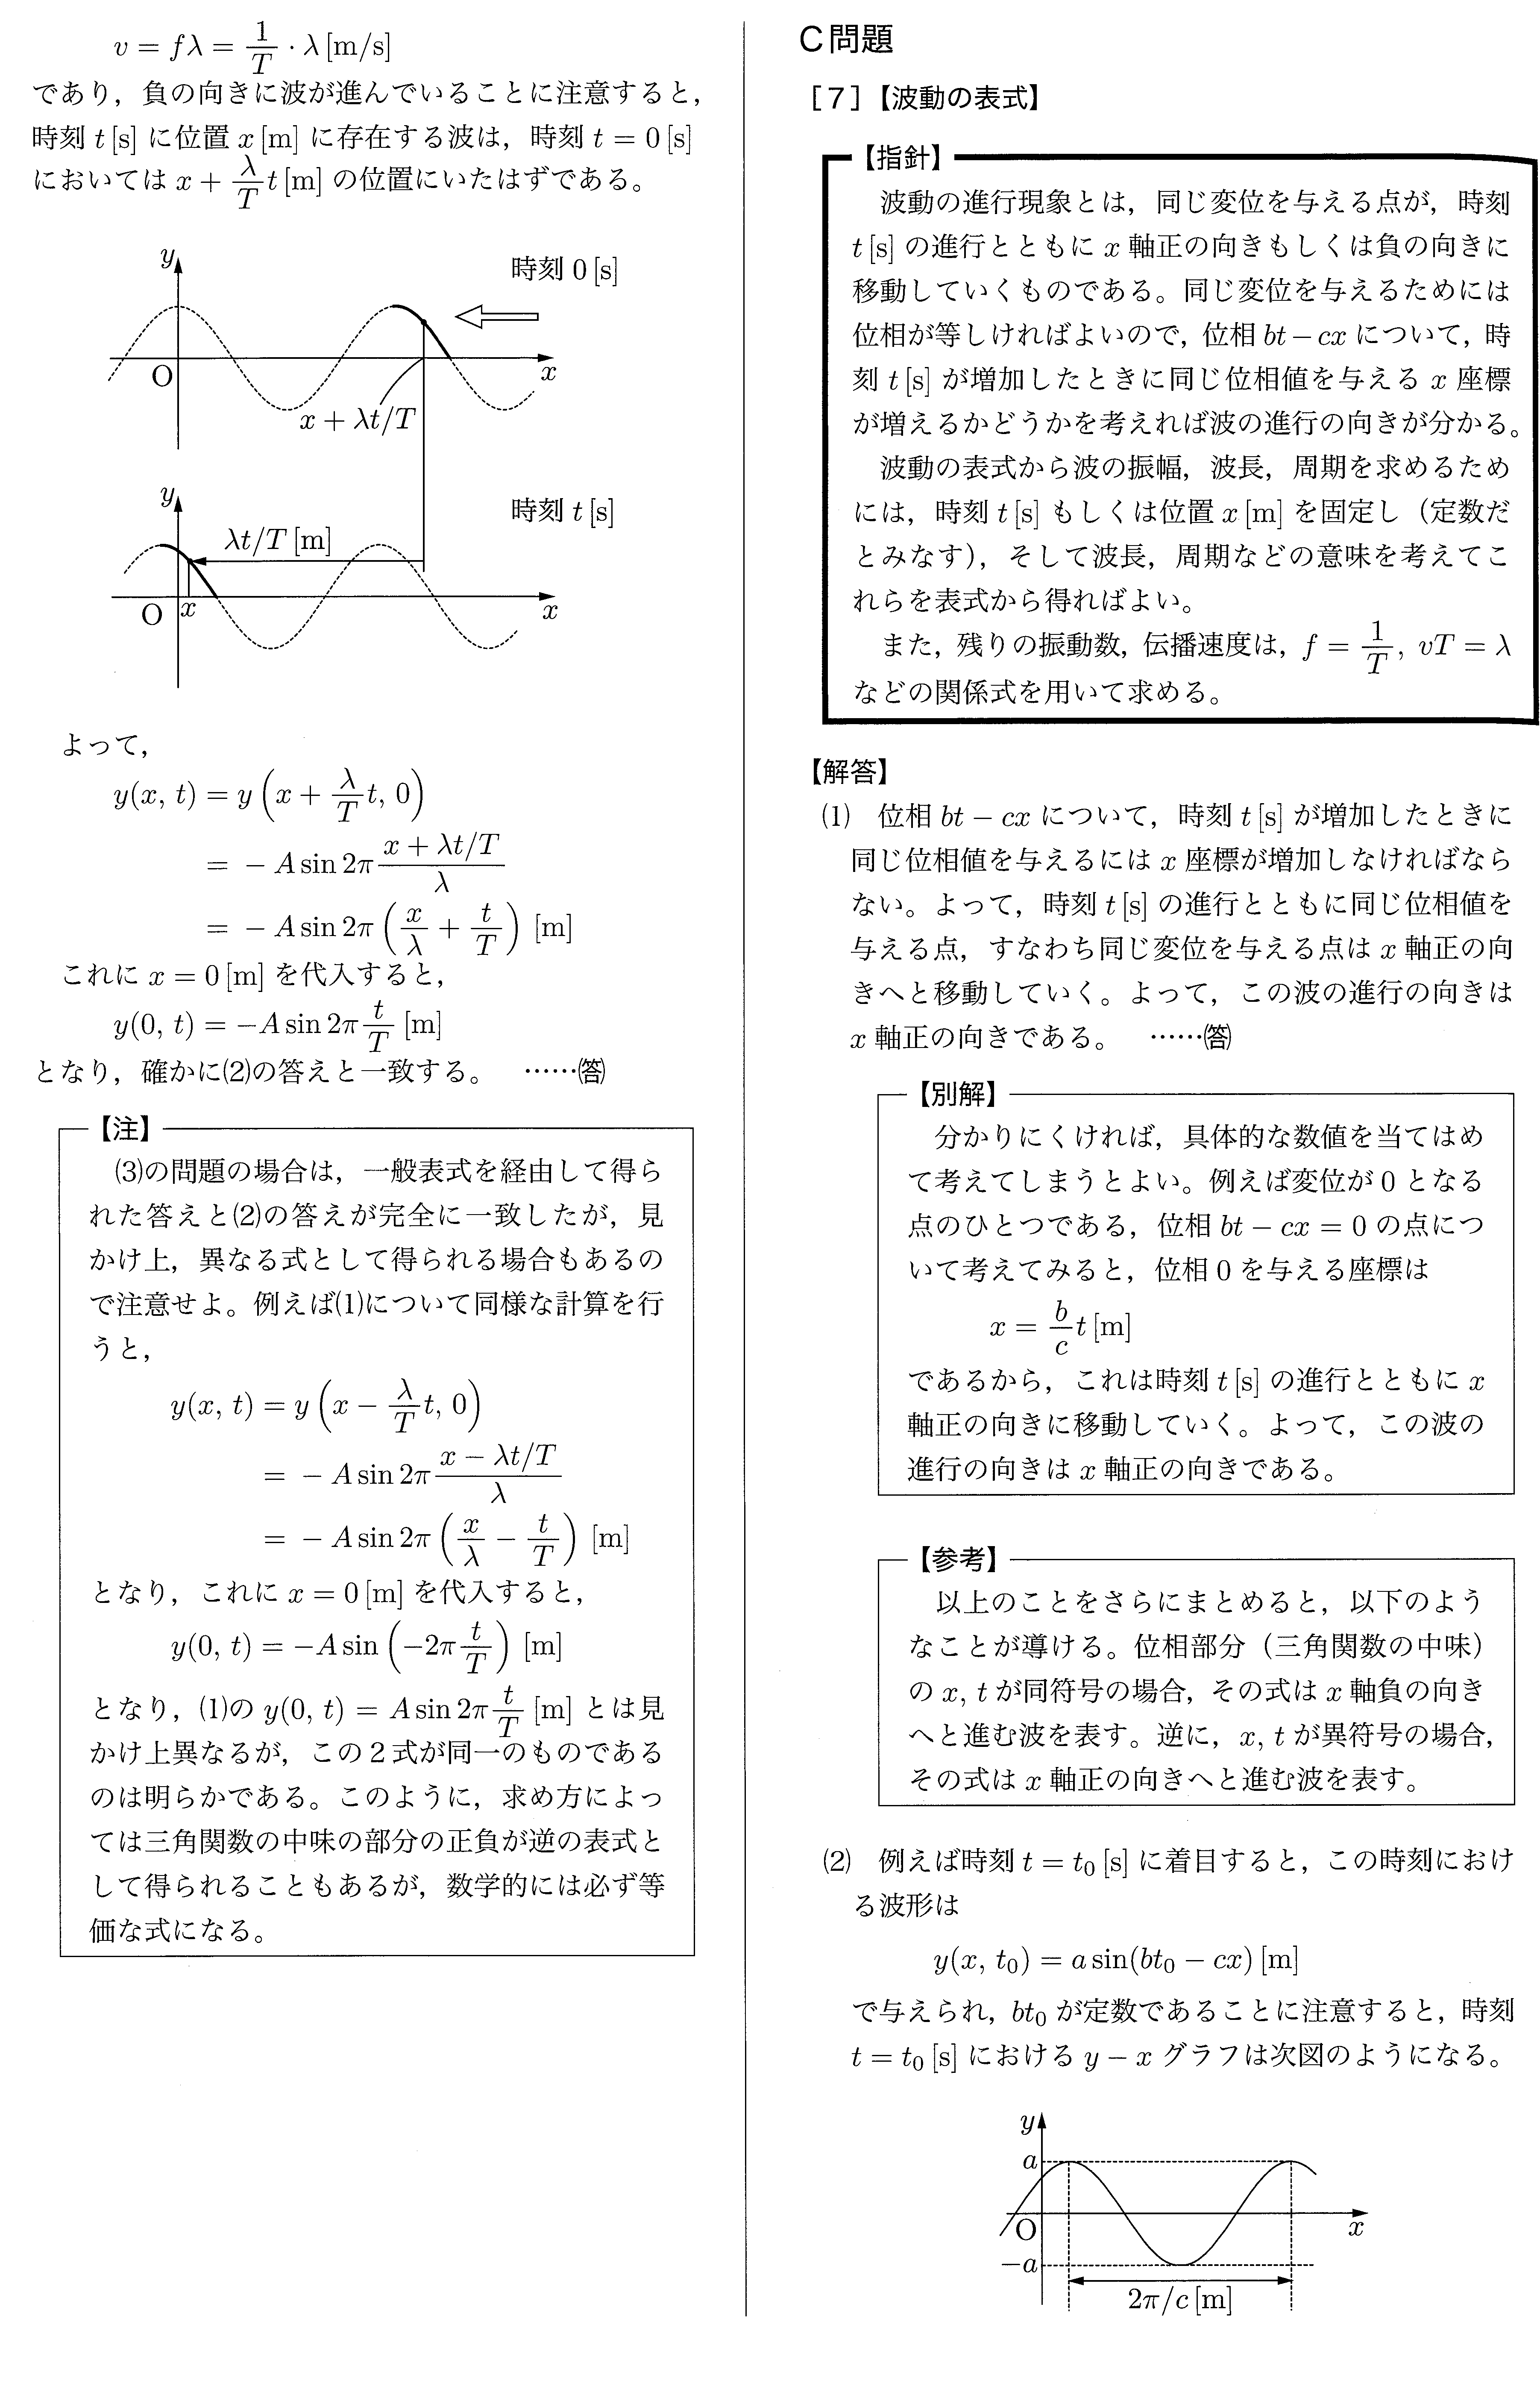
\includegraphics[width=170mm]{prob_p146.png}
\end{center}
\end{figure}

\newpage

\begin{figure}[h]
\begin{center}
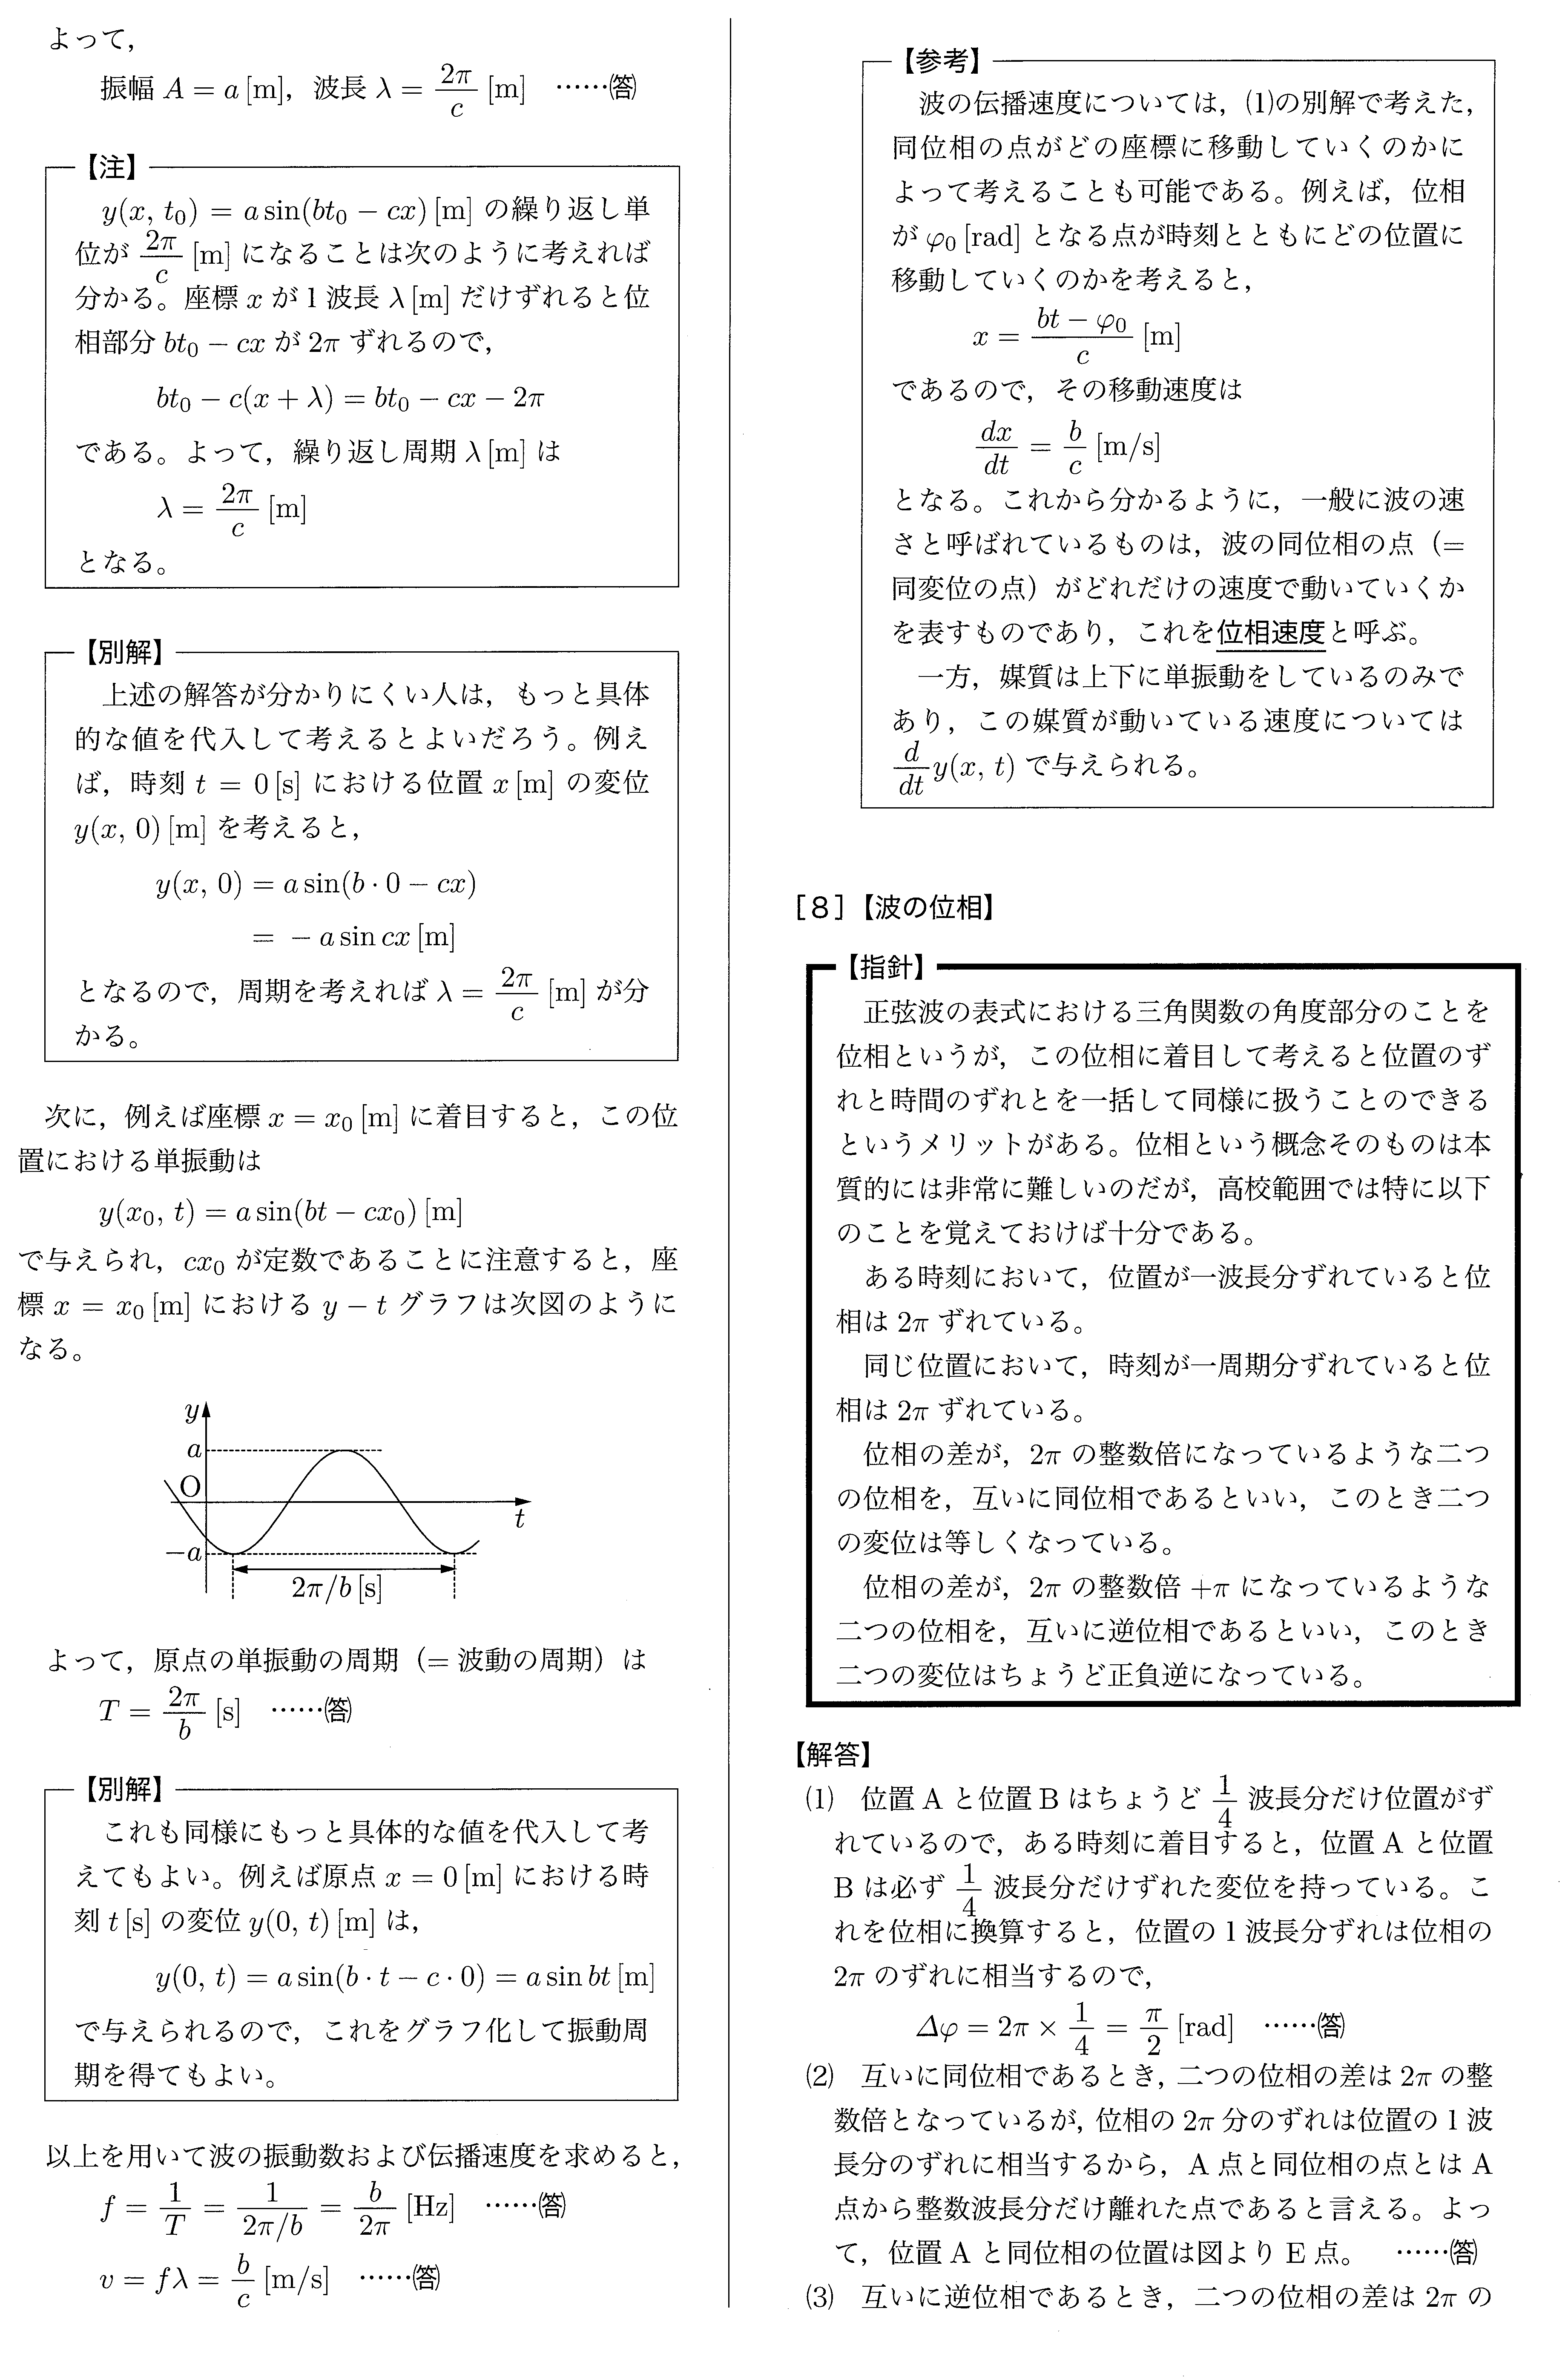
\includegraphics[width=170mm]{prob_p147.png}
\end{center}
\end{figure}

\newpage

\begin{figure}[h]
\begin{center}
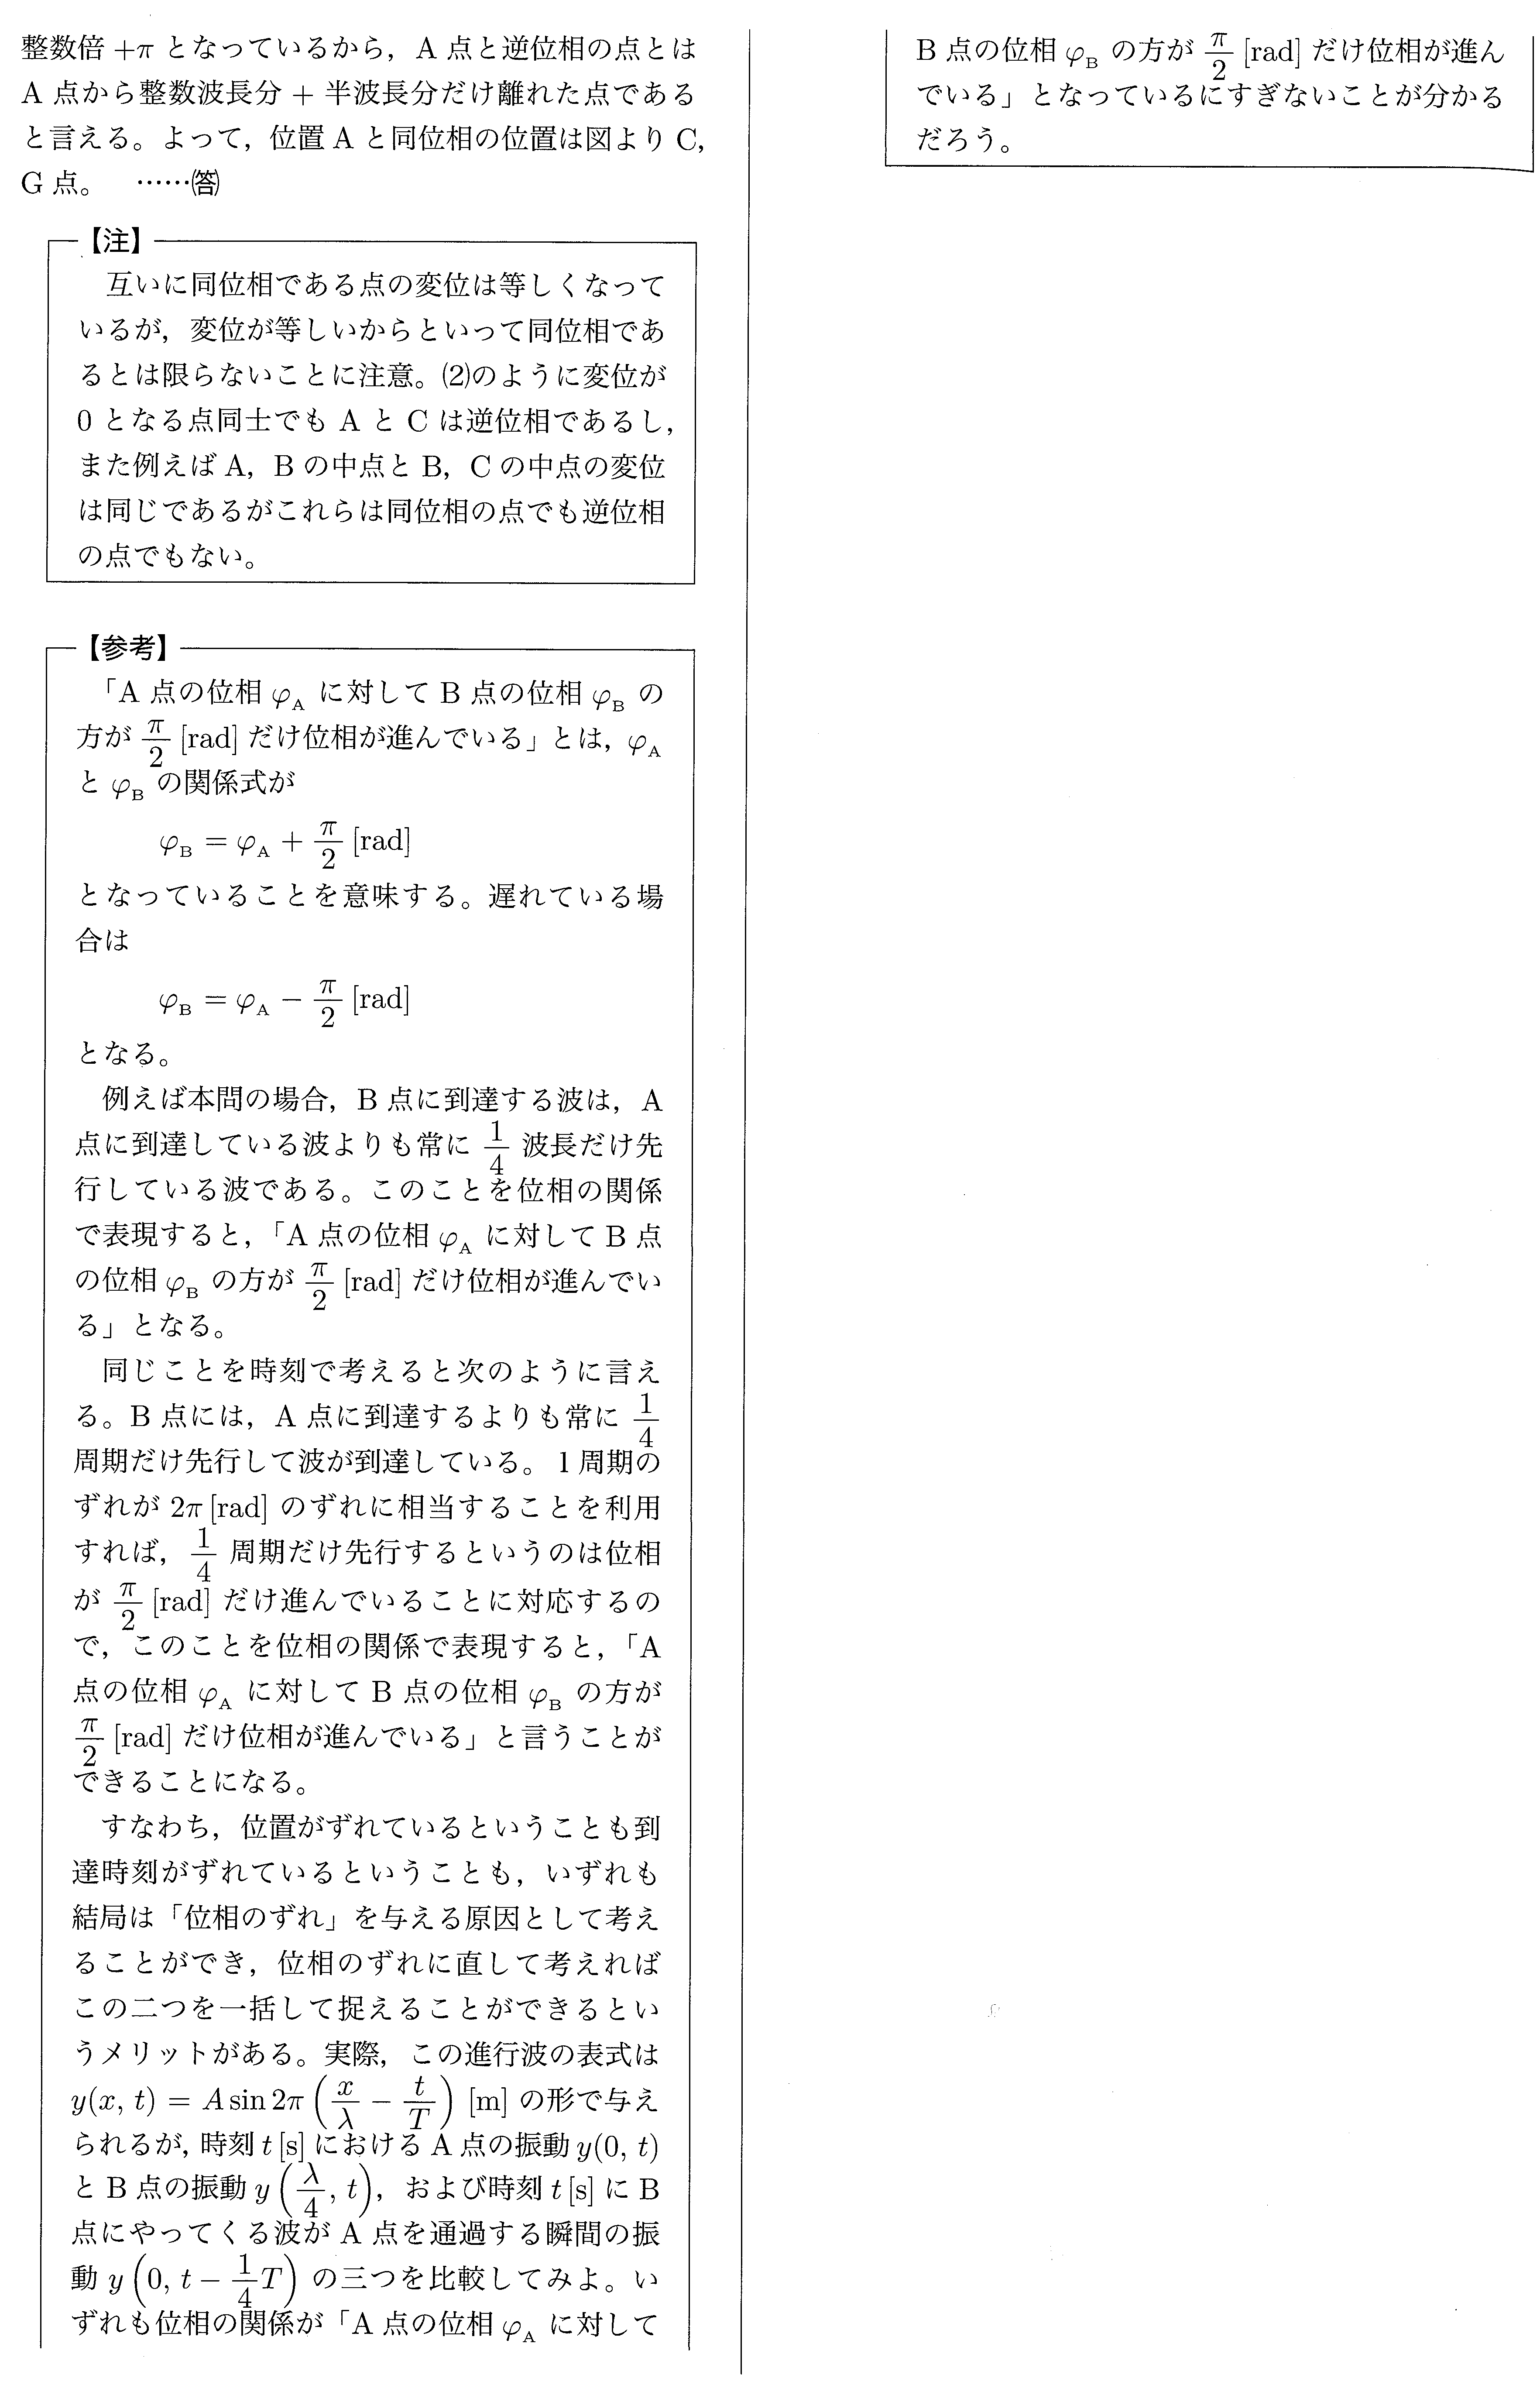
\includegraphics[width=170mm]{prob_p148.png}
\end{center}
\end{figure}

 \ 
 
\newpage
\section{波動の干渉}

\subsection{縦波}
弦の振動のように，波の進行方向に対して垂直な方向に媒質が振動する波を{\bf 横波}と呼ぶ．
波にはこの横波の他に，波の進行方向と平行に媒質が振動する波である{\bf 縦波}がある．

\begin{wrapfigure}[18]{r}[5mm]{120mm}
  \centering
  \vspace{-5mm}
  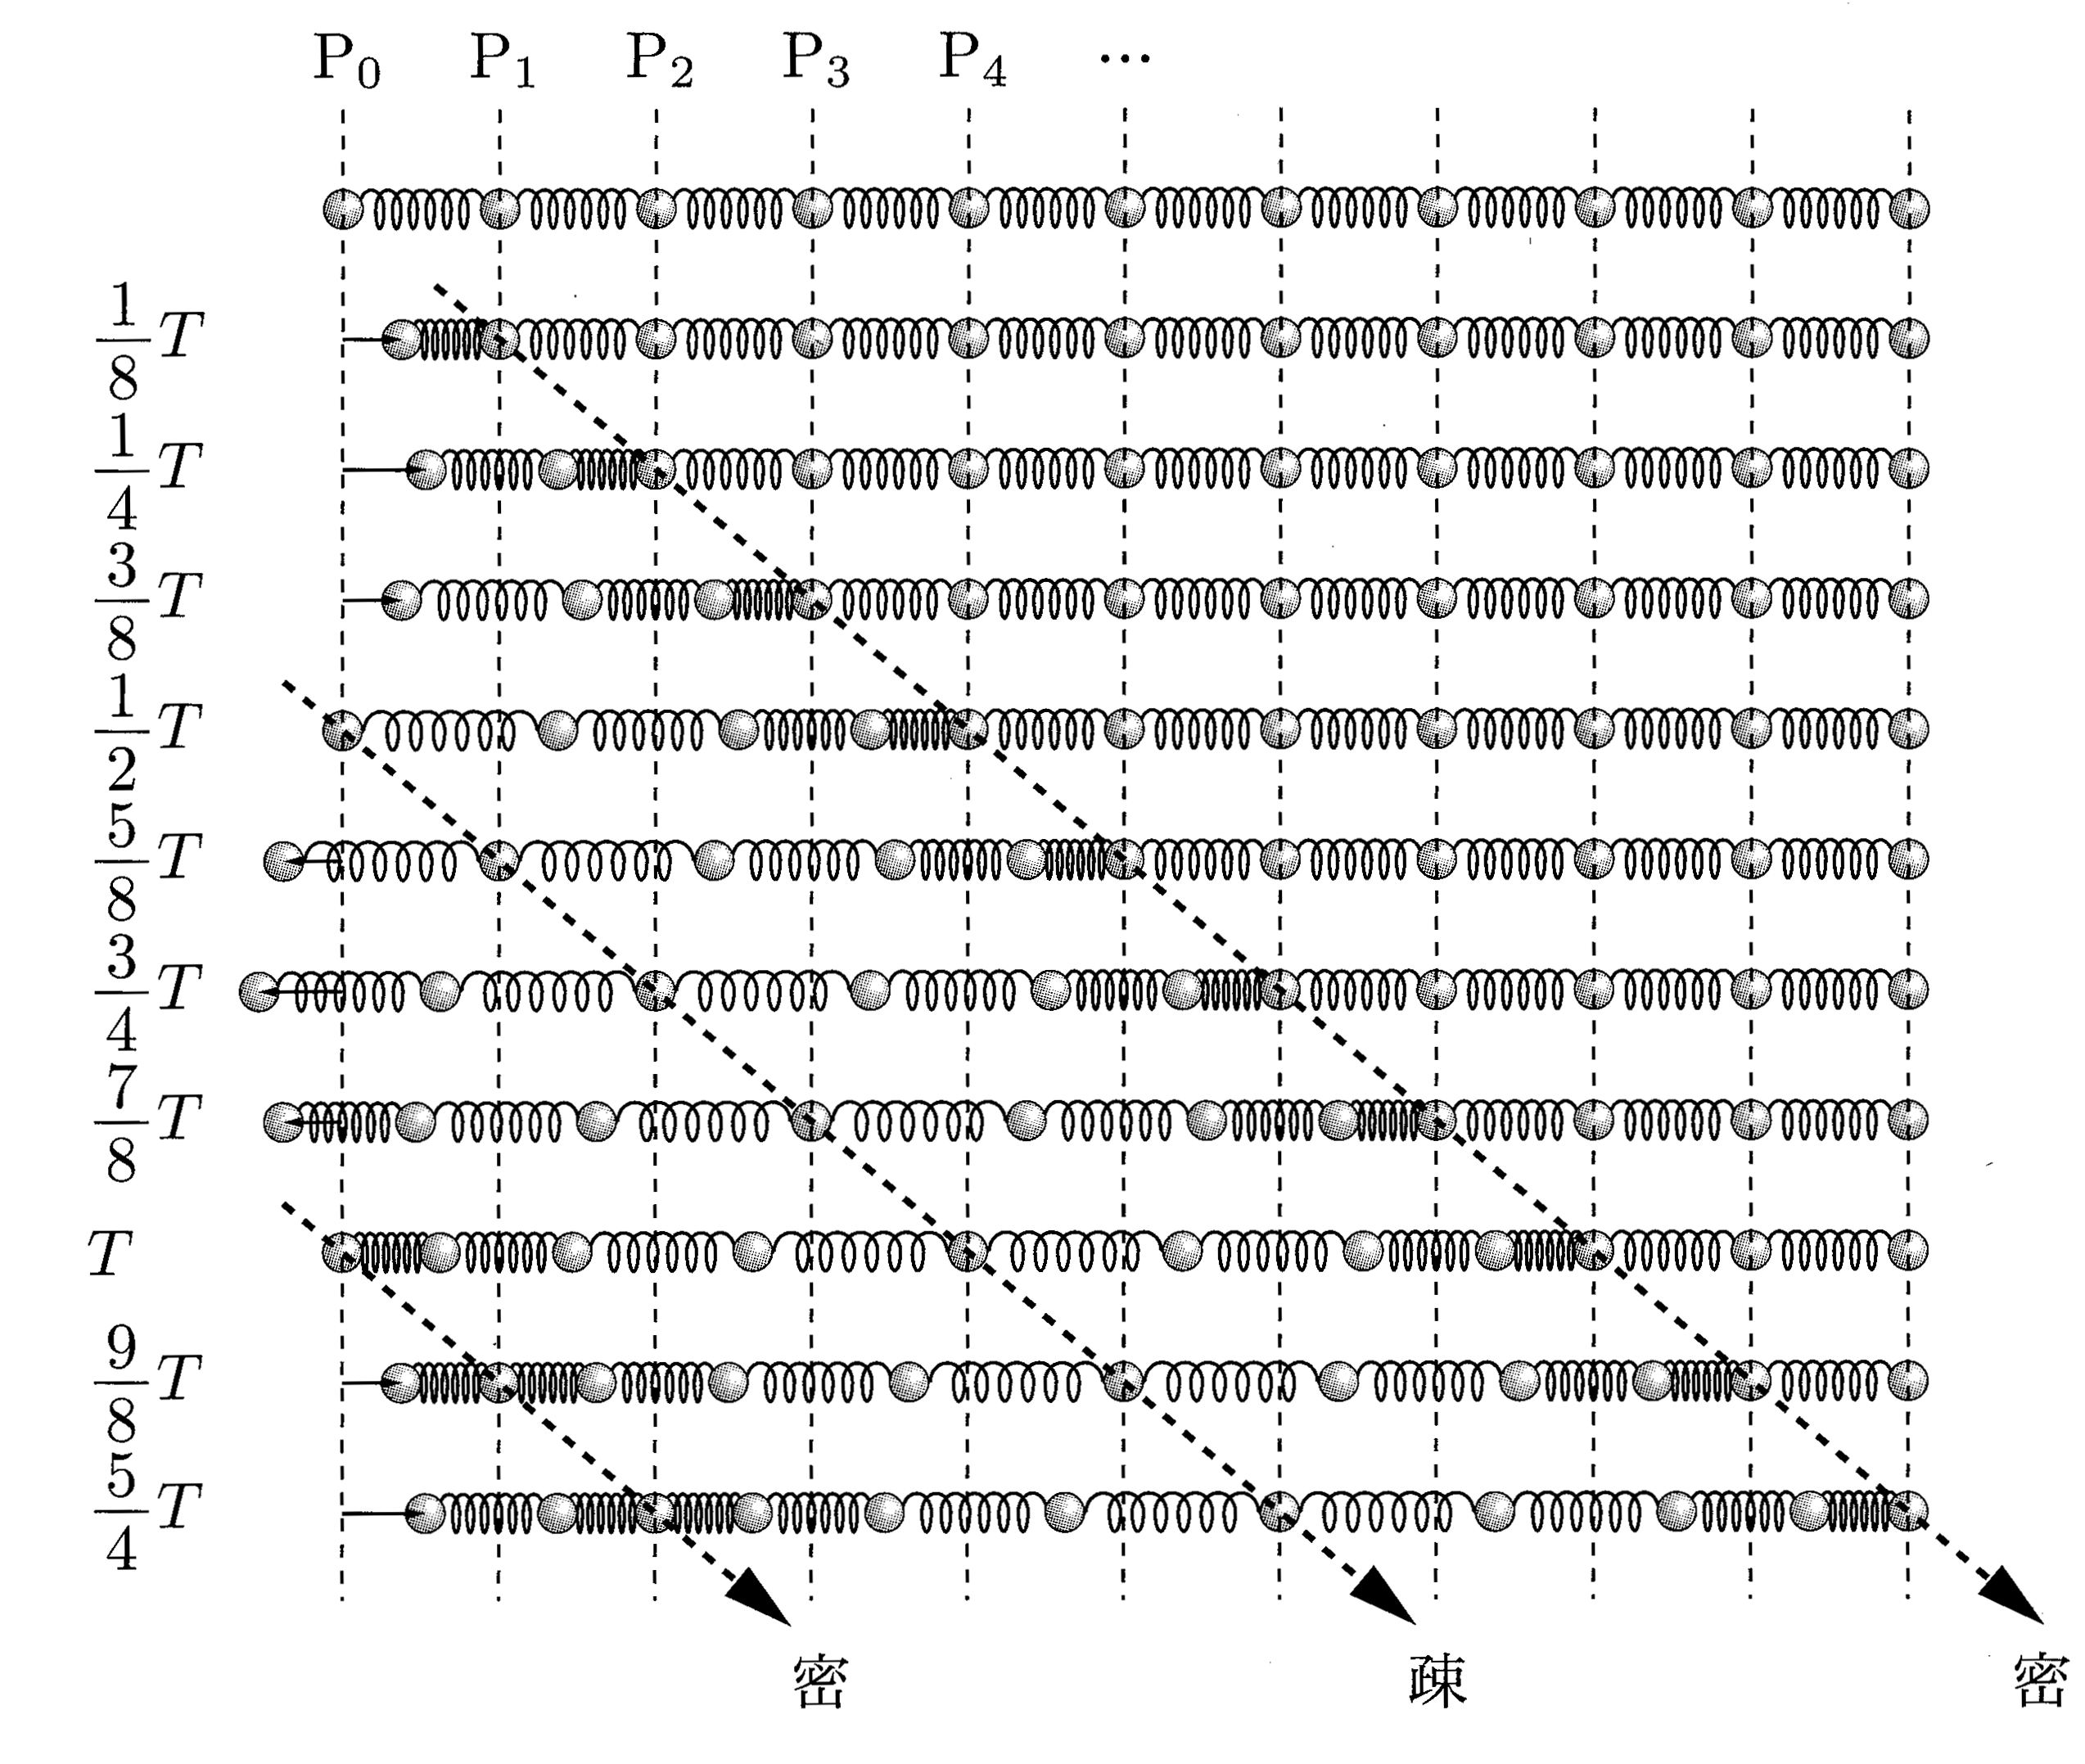
\includegraphics[keepaspectratio,width=120mm]
  {text_p91_fig1.png}
\end{wrapfigure}
縦波を理解するためには図のような等しい質量をもつ小球と等しいバネとが連結されて水平面上に置かれている状況を考えるとよい．

この図において，一番左端の小球$P_0$を左右に単振動させると，$P_0$の振動につられて$P_1$が動き出し，それにつられて$P_2$が，というように$P_0$の振動が右方向に順に伝わっていく．
$P_0$の単振動が右端に達して左に戻ると，それにつられて$P_1$も左へ，$P_2$も，というように振動するため，各小球は初期位置を中心とすに波の進行方向と平行な方向に振動する．
このように，{\bf 媒質の振動方向と平行に振動が伝播する波のことを縦波という．}

各小球は少しずつ時間がずれて単振動するため，小球が集まって密度が高くなる部分（密部）と，小球が離れて密度が低くなる部分（疎部）とができ，これらの密部，疎部が波の進行方向へ一定の速さで伝播していく．
そのため，縦波は疎密波と呼ばれることもある．

\begin{wrapfigure}[10]{r}[5mm]{60mm}
  \centering
  \vspace{-5mm}
  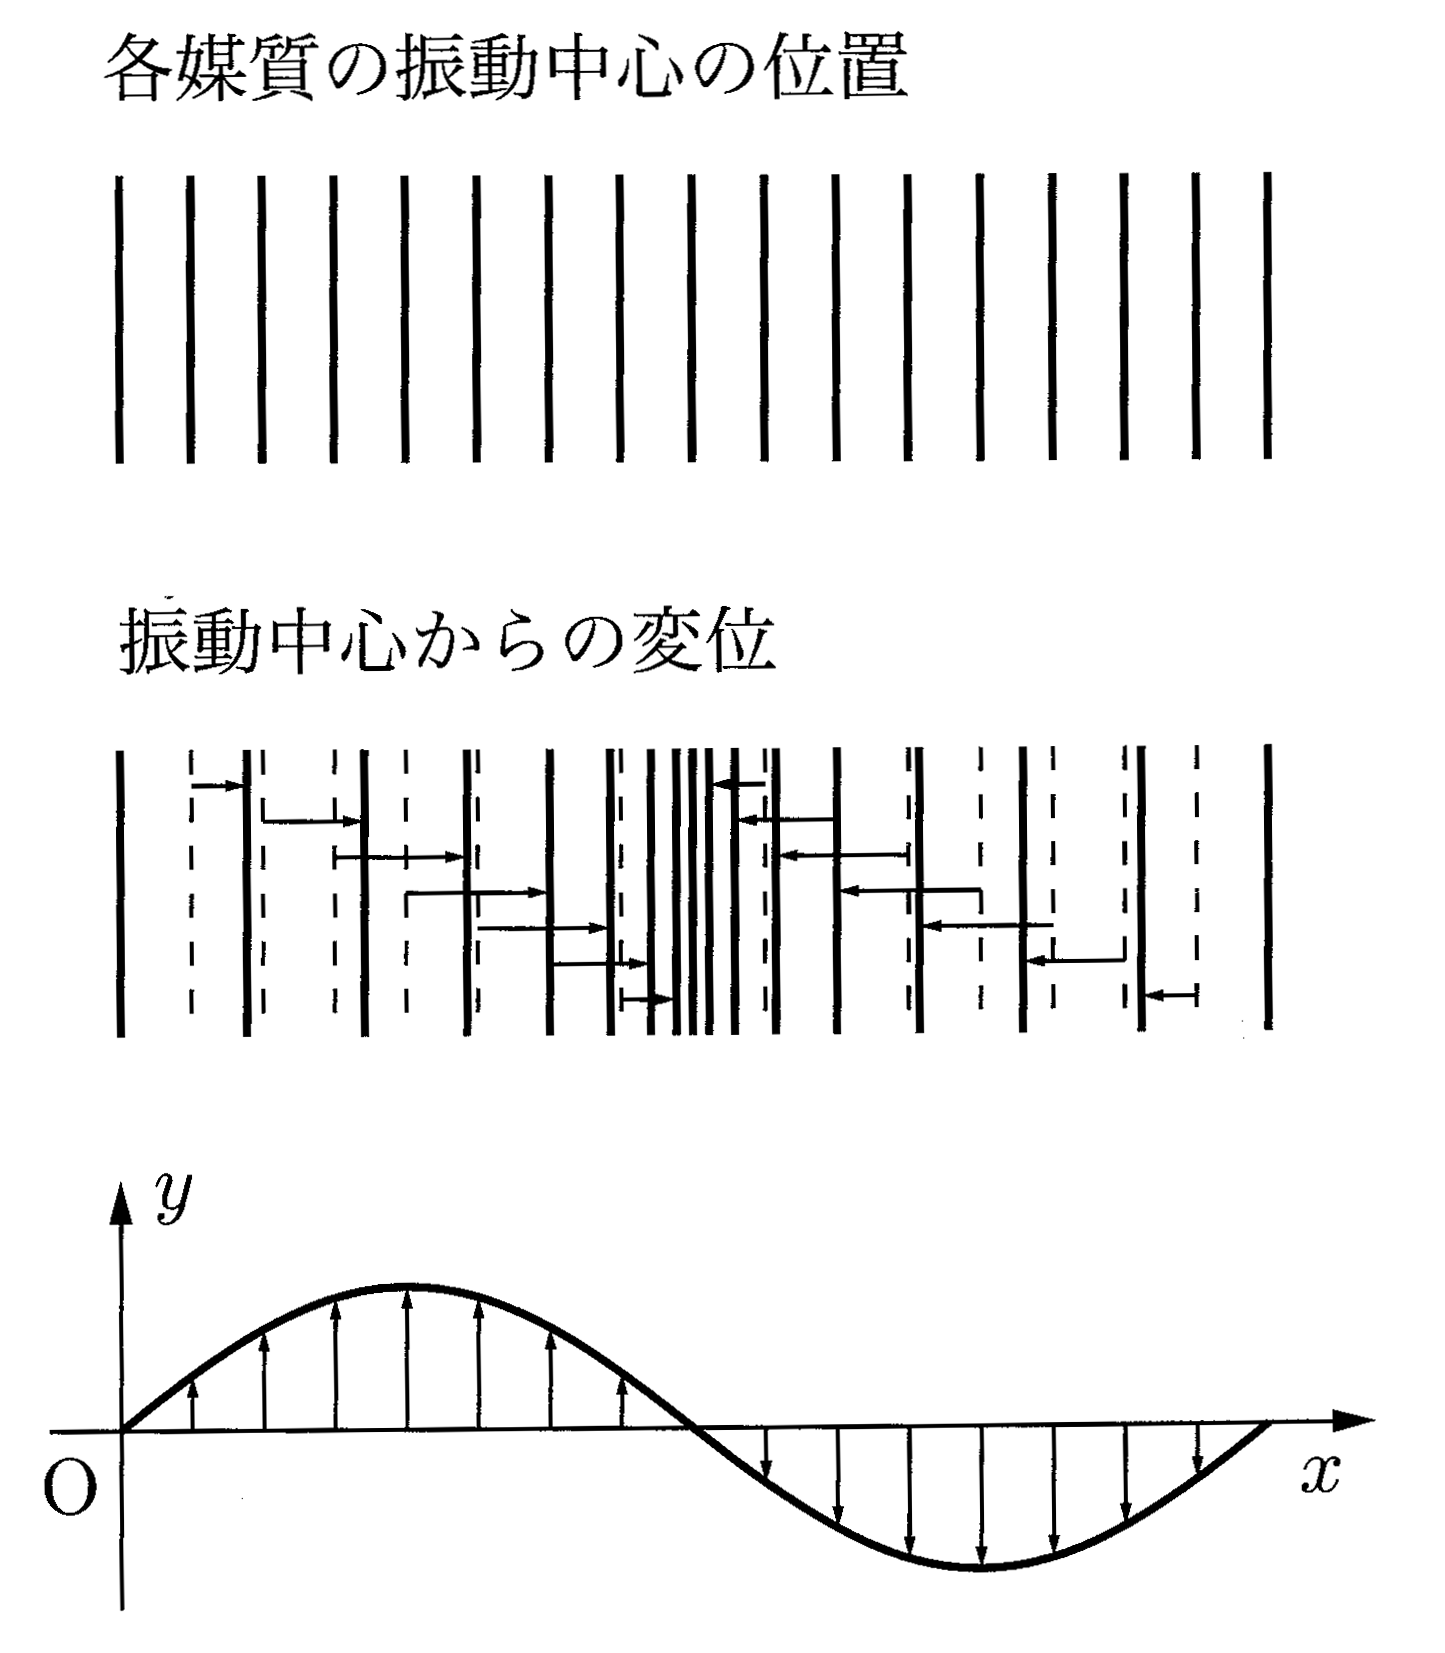
\includegraphics[keepaspectratio,width=60mm]
  {text_p91_fig2.png}
\end{wrapfigure}
縦波の各点の振動は波の伝搬方向と一致しているため，そのまま図示すると分かりにくい．
そこで，振動中心からの変位を縦軸にしたグラフを用いることが多い．
この際，{\bf 媒質の変位は初期位置からの変位を反時計回りに90度回転させて図示すればよい．}
媒質が$x$軸正の向きに変位したときに，$y$軸正の向きに変位を取るようにして図示するとちょうど横波と同様な$y-x$グラフとなるため，数式的には横波と同様にして扱うことができる．
これを{\bf 縦波の横波表示}という．
横波表示された縦波の媒質の各点の変位を実際の変位に戻すためには，$y$軸正の向きの変位を時計回りに90度回転させて，$x$軸正の向きの変位に直せばよい．

\vspace{15mm}
\begin{matome}{正弦波}
 \hspace{3mm} 横波：波の進行方向と媒質の変位方向が垂直であるもの．水面波，弦の振動など．\\
\hspace{3mm} 縦波：波の進行方向と媒質の変位方向が平行であるもの．疎密波とも呼ばれる．音波など．
 \end{matome}

\subsection{波の独立性と干渉による強め合い・弱め合い}
\begin{wrapfigure}[6]{r}[5mm]{35mm}
  \centering
  \vspace{-5mm}
  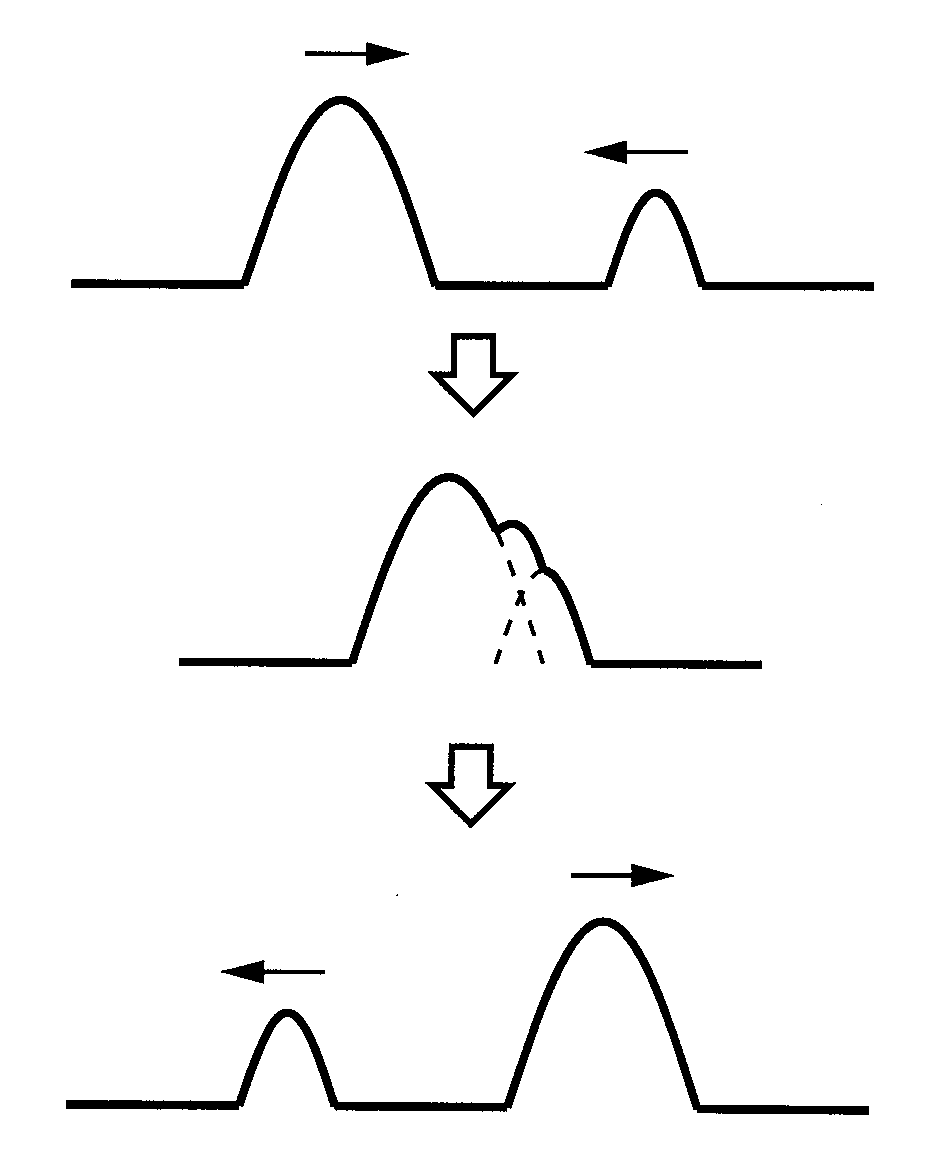
\includegraphics[keepaspectratio,width=35mm]
  {text_p92_fig1.png}
\end{wrapfigure}
1つの媒質上のある1点に2つの波が同時に伝わってきたときには，その点の変位は各々が単独で届いたときの変位$y_1$，$y_2$の代数和$y_1+y_2$となることが知られている．
これを波の{\bf 重ね合わせの原理}という．

このように，2つの波が1つの媒質中で重なるときには各々の波が同時に1つの媒質中を進むだけで，互いの波の進行を妨げたり，影響を及ぼしたりすることがない．
この性質を{\bf 波の独立性}という．

\vspace{15mm}
\begin{wrapfigure}[10]{r}[5mm]{90mm}
  \centering
  \vspace{-5mm}
  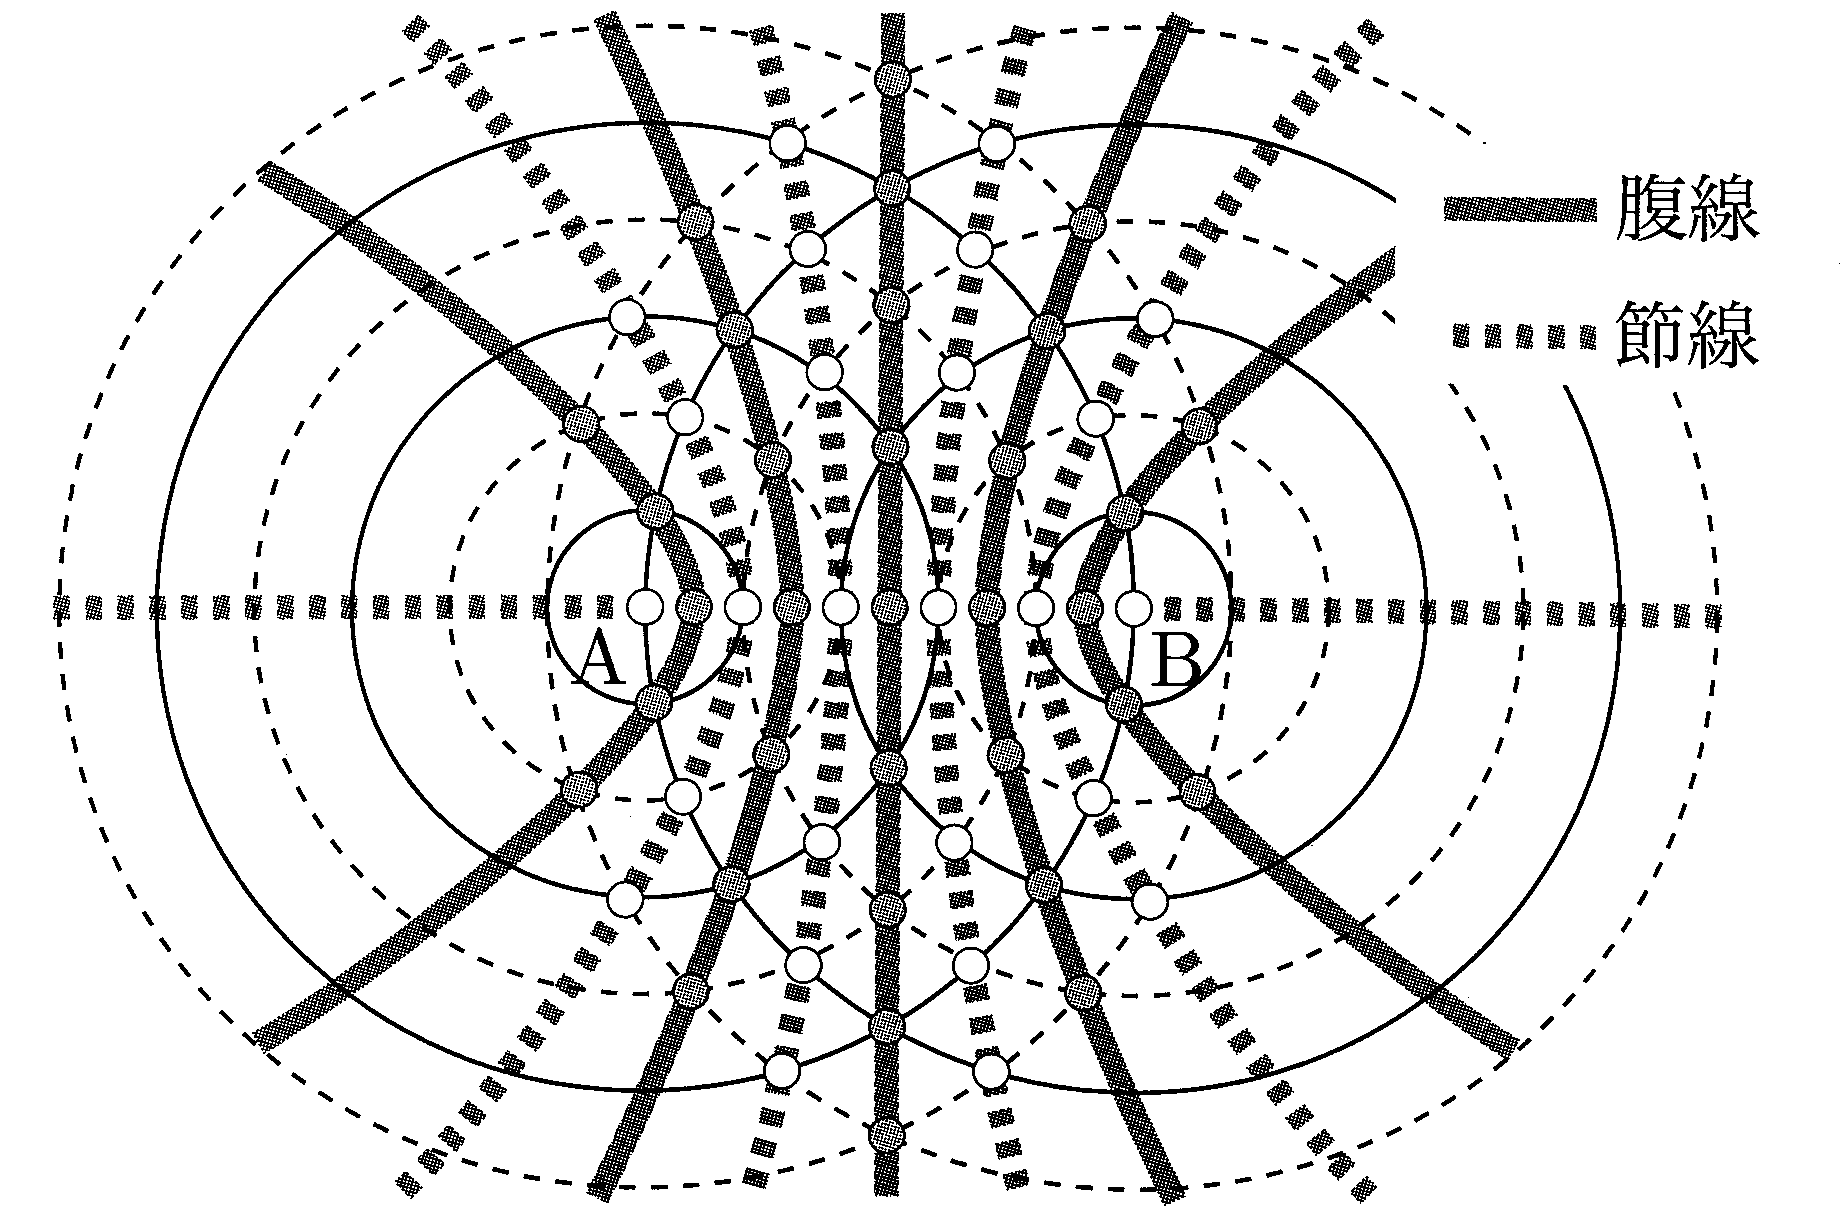
\includegraphics[keepaspectratio,width=90mm]
  {text_p92_fig2.png}
\end{wrapfigure}
さて，水面上の2点A,Bを同周期，同振幅，同変位（=同位相）で連続的に振動させると，水面にはA,B点から円形に波が伝わっていき，水面上でそれらが重ね合わせの原理に従って重なり合う．
各波源で発生した波は山と谷とが交互に送り出され，重なり合った結果として水面上にできる合成波では，
\begin{description}
\item[・] Aからの波の振動とBからの波の振動が同位相で重なるために2つの波が強めあって大きく振動する点（腹）
\item[・] Aからの波の振動とBからの波の振動が逆位相で重なるために2つの波が弱めあって全く振動しない点（節）
\end{description}
が作られる．
これらの点は連続的に連なって分布しているために曲線となり，前者を腹線，後者を節線という．

\begin{wrapfigure}[6]{r}[5mm]{40mm}
  \centering
  \vspace{-5mm}
  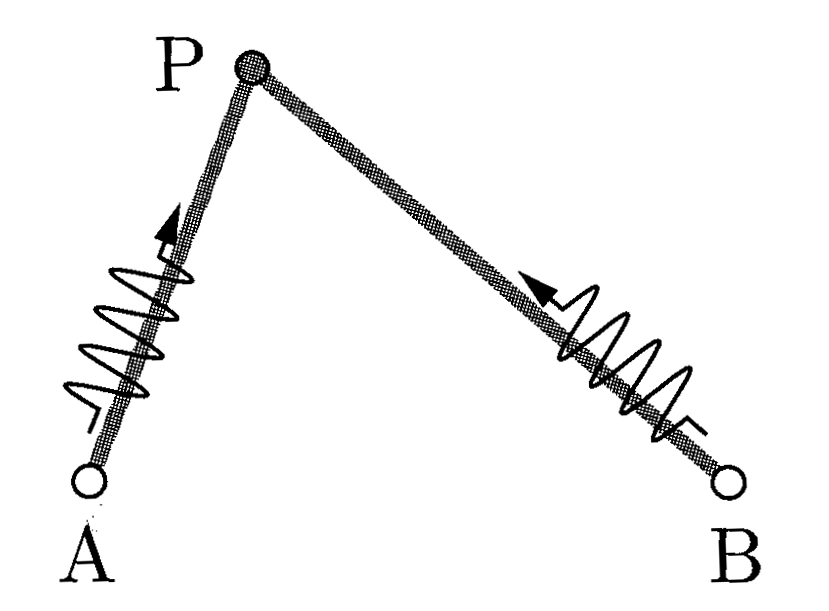
\includegraphics[keepaspectratio,width=40mm]
  {text_p93_fig1.png}
\end{wrapfigure}
平面上のある点で2つの異なる波源からやってきた波が強め合うか弱め合うかは，
\begin{description}
\item[\MARU{1}] 2つの波源の振動の位相差
\item[\MARU{2}] 2つの波源の距離の差
\end{description}
の2つによって決定される．
まず簡単のため，2つの波源の振動が全く同じ（=位相差がない）場合について考える．

A点とB点からの距離の差がちょうど1波長$\lambda$[m]の整数倍になっているような点Pの場合，2つの波源から点Pに向かってやってくる波を横に並べて描いてみると，P点には常に同一の変位が届いていることがわかる．
よって，2つの変位を足し合わせたものは1つの変位の倍になる．
これを互いに{\bf 強め合っている}といい，このときP点は大きく振動することになる．
 \begin{figure}[h]
\begin{center}
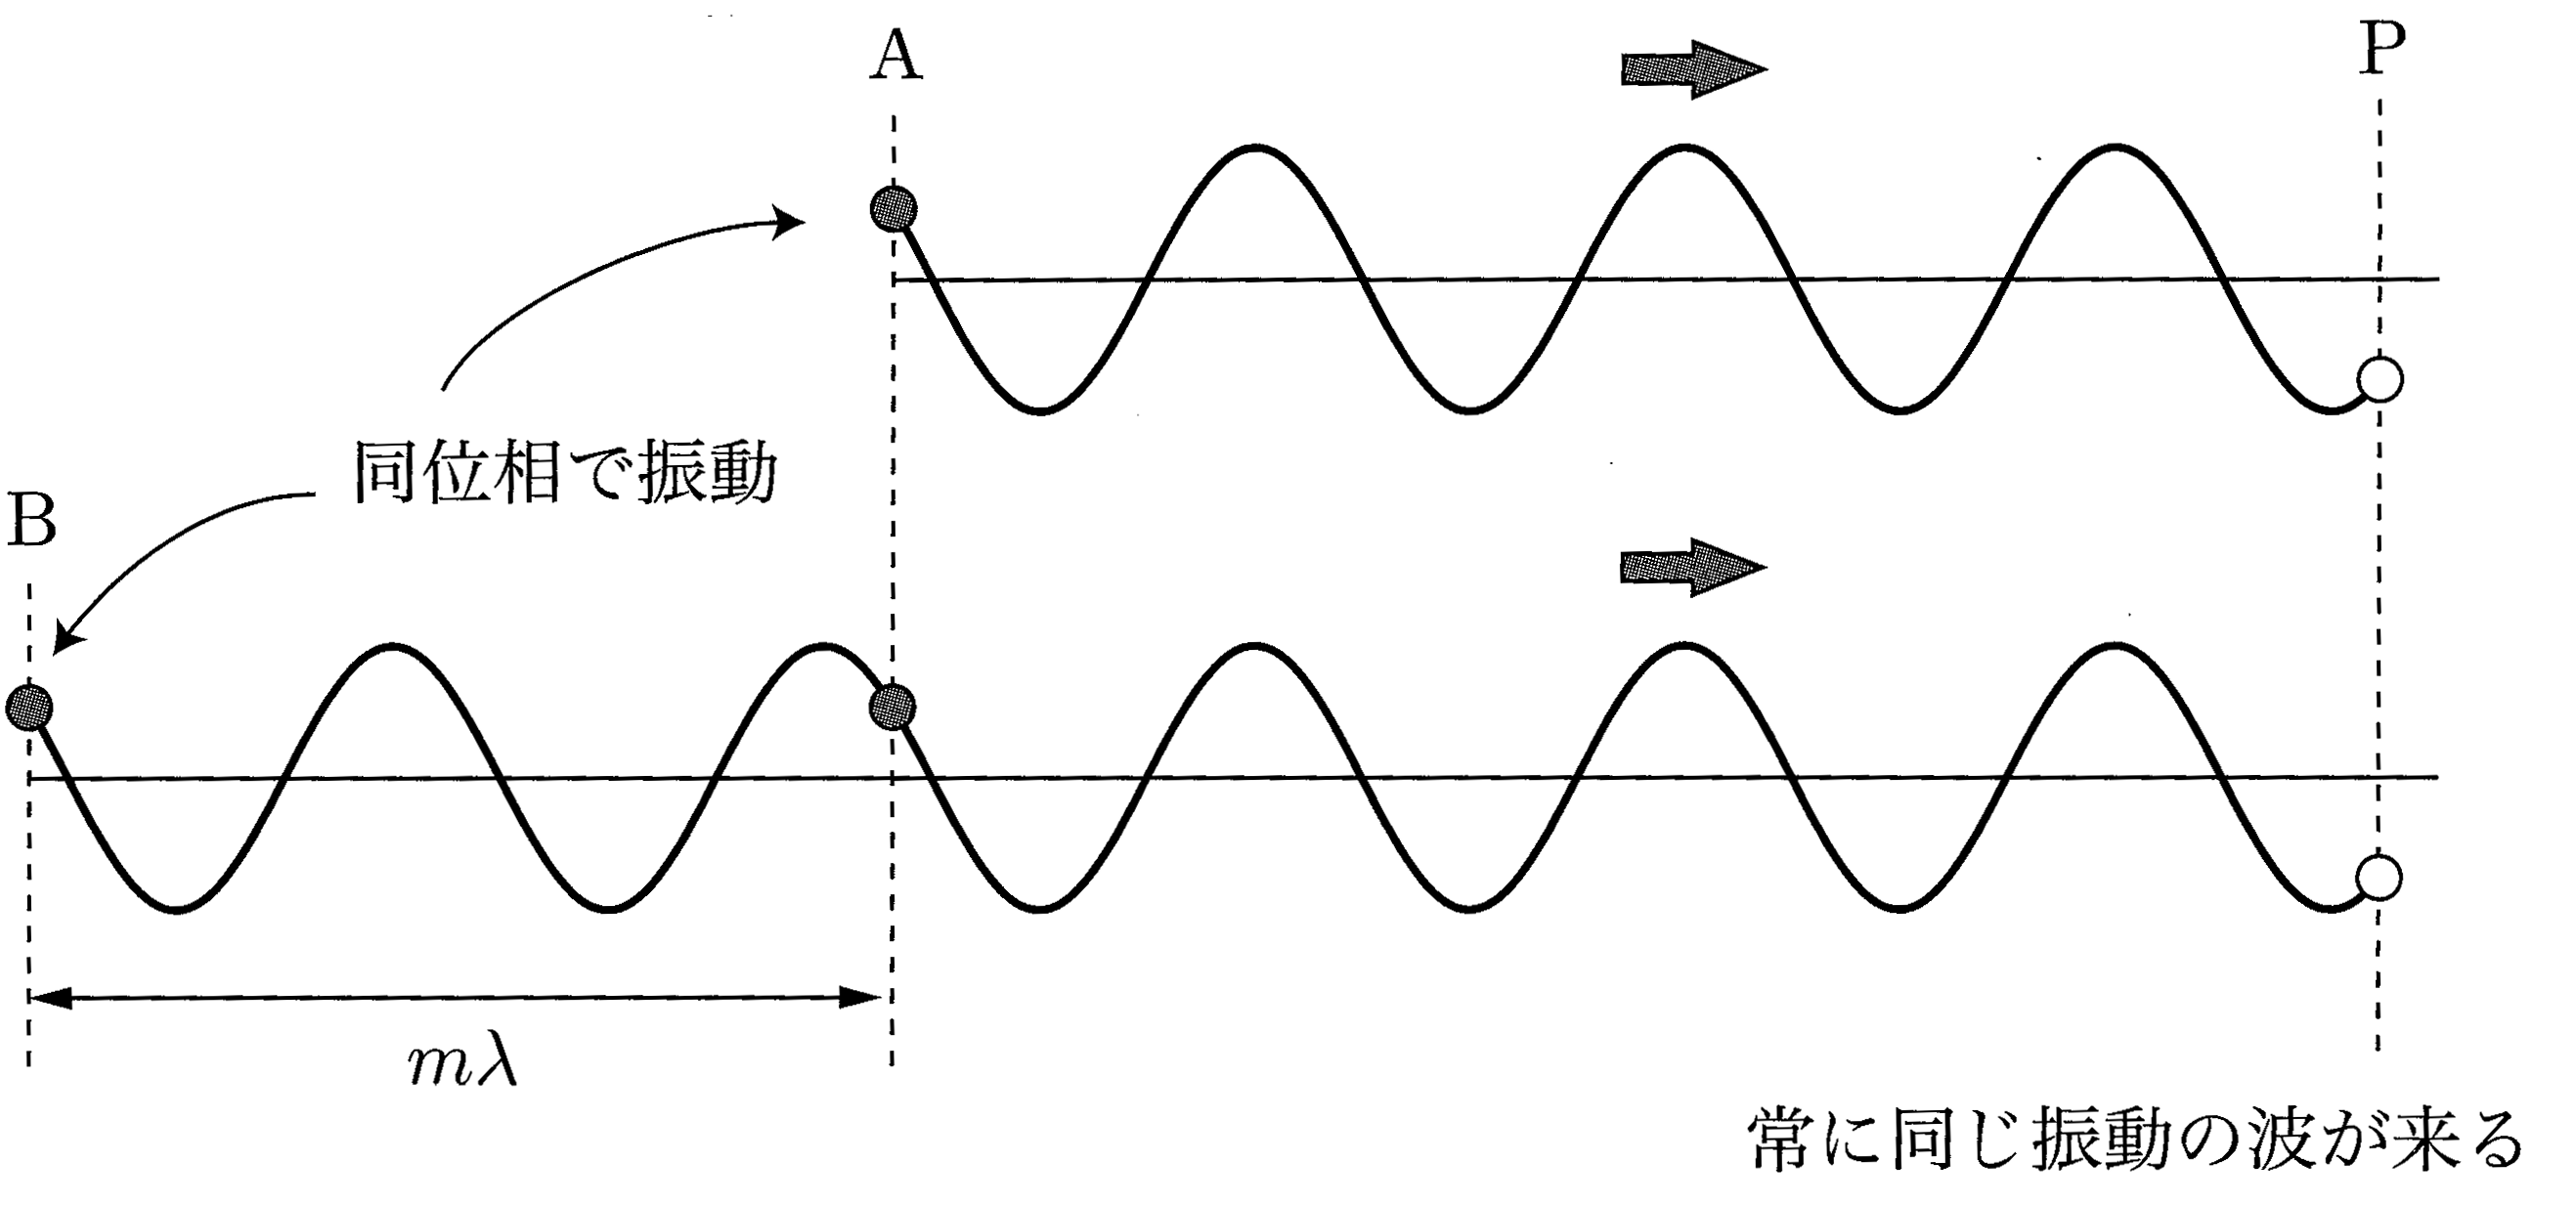
\includegraphics[width=120mm]{text_p93_fig2.png}
\end{center}
\end{figure}

\vspace{50mm}
また，A点とB点からの距離の差がちょうど1波長$\lambda$[m]の$m-\dfrac{1}{2}$倍（$m$は整数）になっているような点Pの場合，2つの波源からやってくる変位は点Pにおいて必ず正負逆の変位をもつ．
よって，2つの変位を足し合わせたものは常に0となり，全く振動しなくなる．
これを互いに{\bf 弱め合っている}といい，このときP点は全く振動しないことになる．

 \begin{figure}[h]
\begin{center}
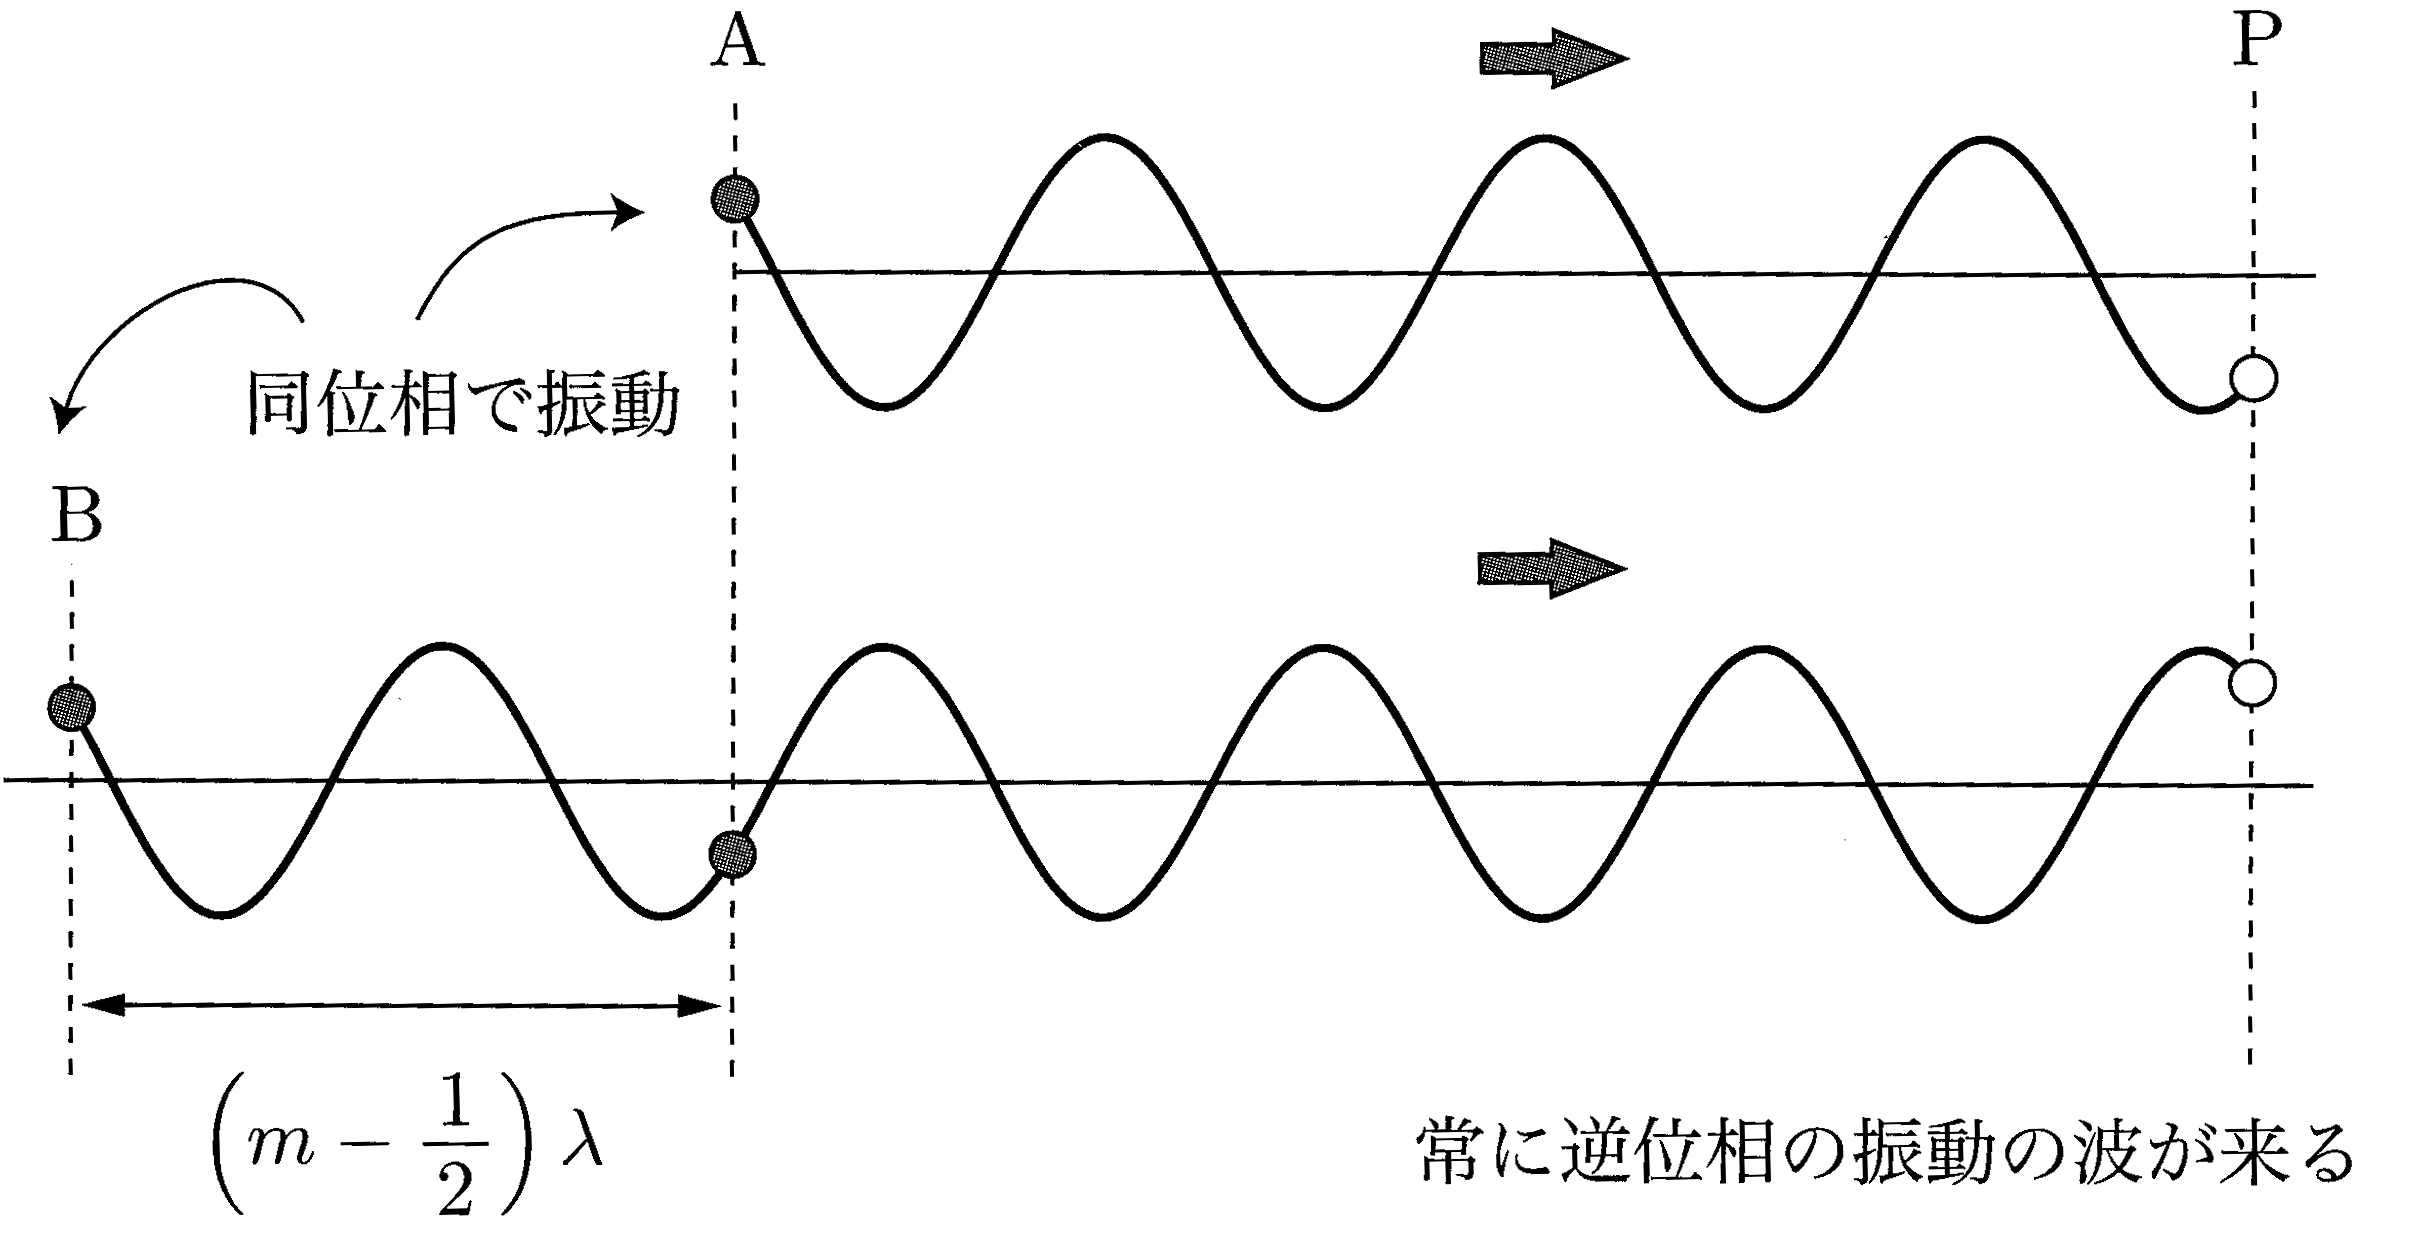
\includegraphics[width=120mm]{text_p93_fig3.png}
\end{center}
\end{figure}

以上より，A，Bからの距離がそれぞれ$r_1,r_2$である点Pが，
\[強め合いとなる条件：r_1-r_2=m\lambda \hspace{5mm}（ただしmは整数）\hspace{13mm}\]
\[弱め合いとなる条件：r_1-r_2=\left( m-\dfrac{1}{2} \right) \lambda \hspace{5mm}（ただしmは整数）\]
であり，これらはそれぞれ水面上で波源の位置を焦点とする双曲線となる．
\begin{matome}{水面波の干渉}
 \hspace{3mm} 波源A,Bが同位相で振動しているとき，2点からの距離がそれぞれ$r_1,r_2$である点Pは
 \[ r_1-r_2=m\lambda \hspace{18mm}のとき強め合い\]
 \[r_1-r_2=\left( m-\dfrac{1}{2} \right)\lambda \hspace{5mm}のとき弱め合い\]
\end{matome}
波源A,Bの振動に位相差がある場合はこれも考慮して強め合い，弱め合いを決定する必要がある．

\newpage
\subsection{定常波}
\begin{wrapfigure}[13]{r}[5mm]{70mm}
  \centering
  \vspace{-5mm}
  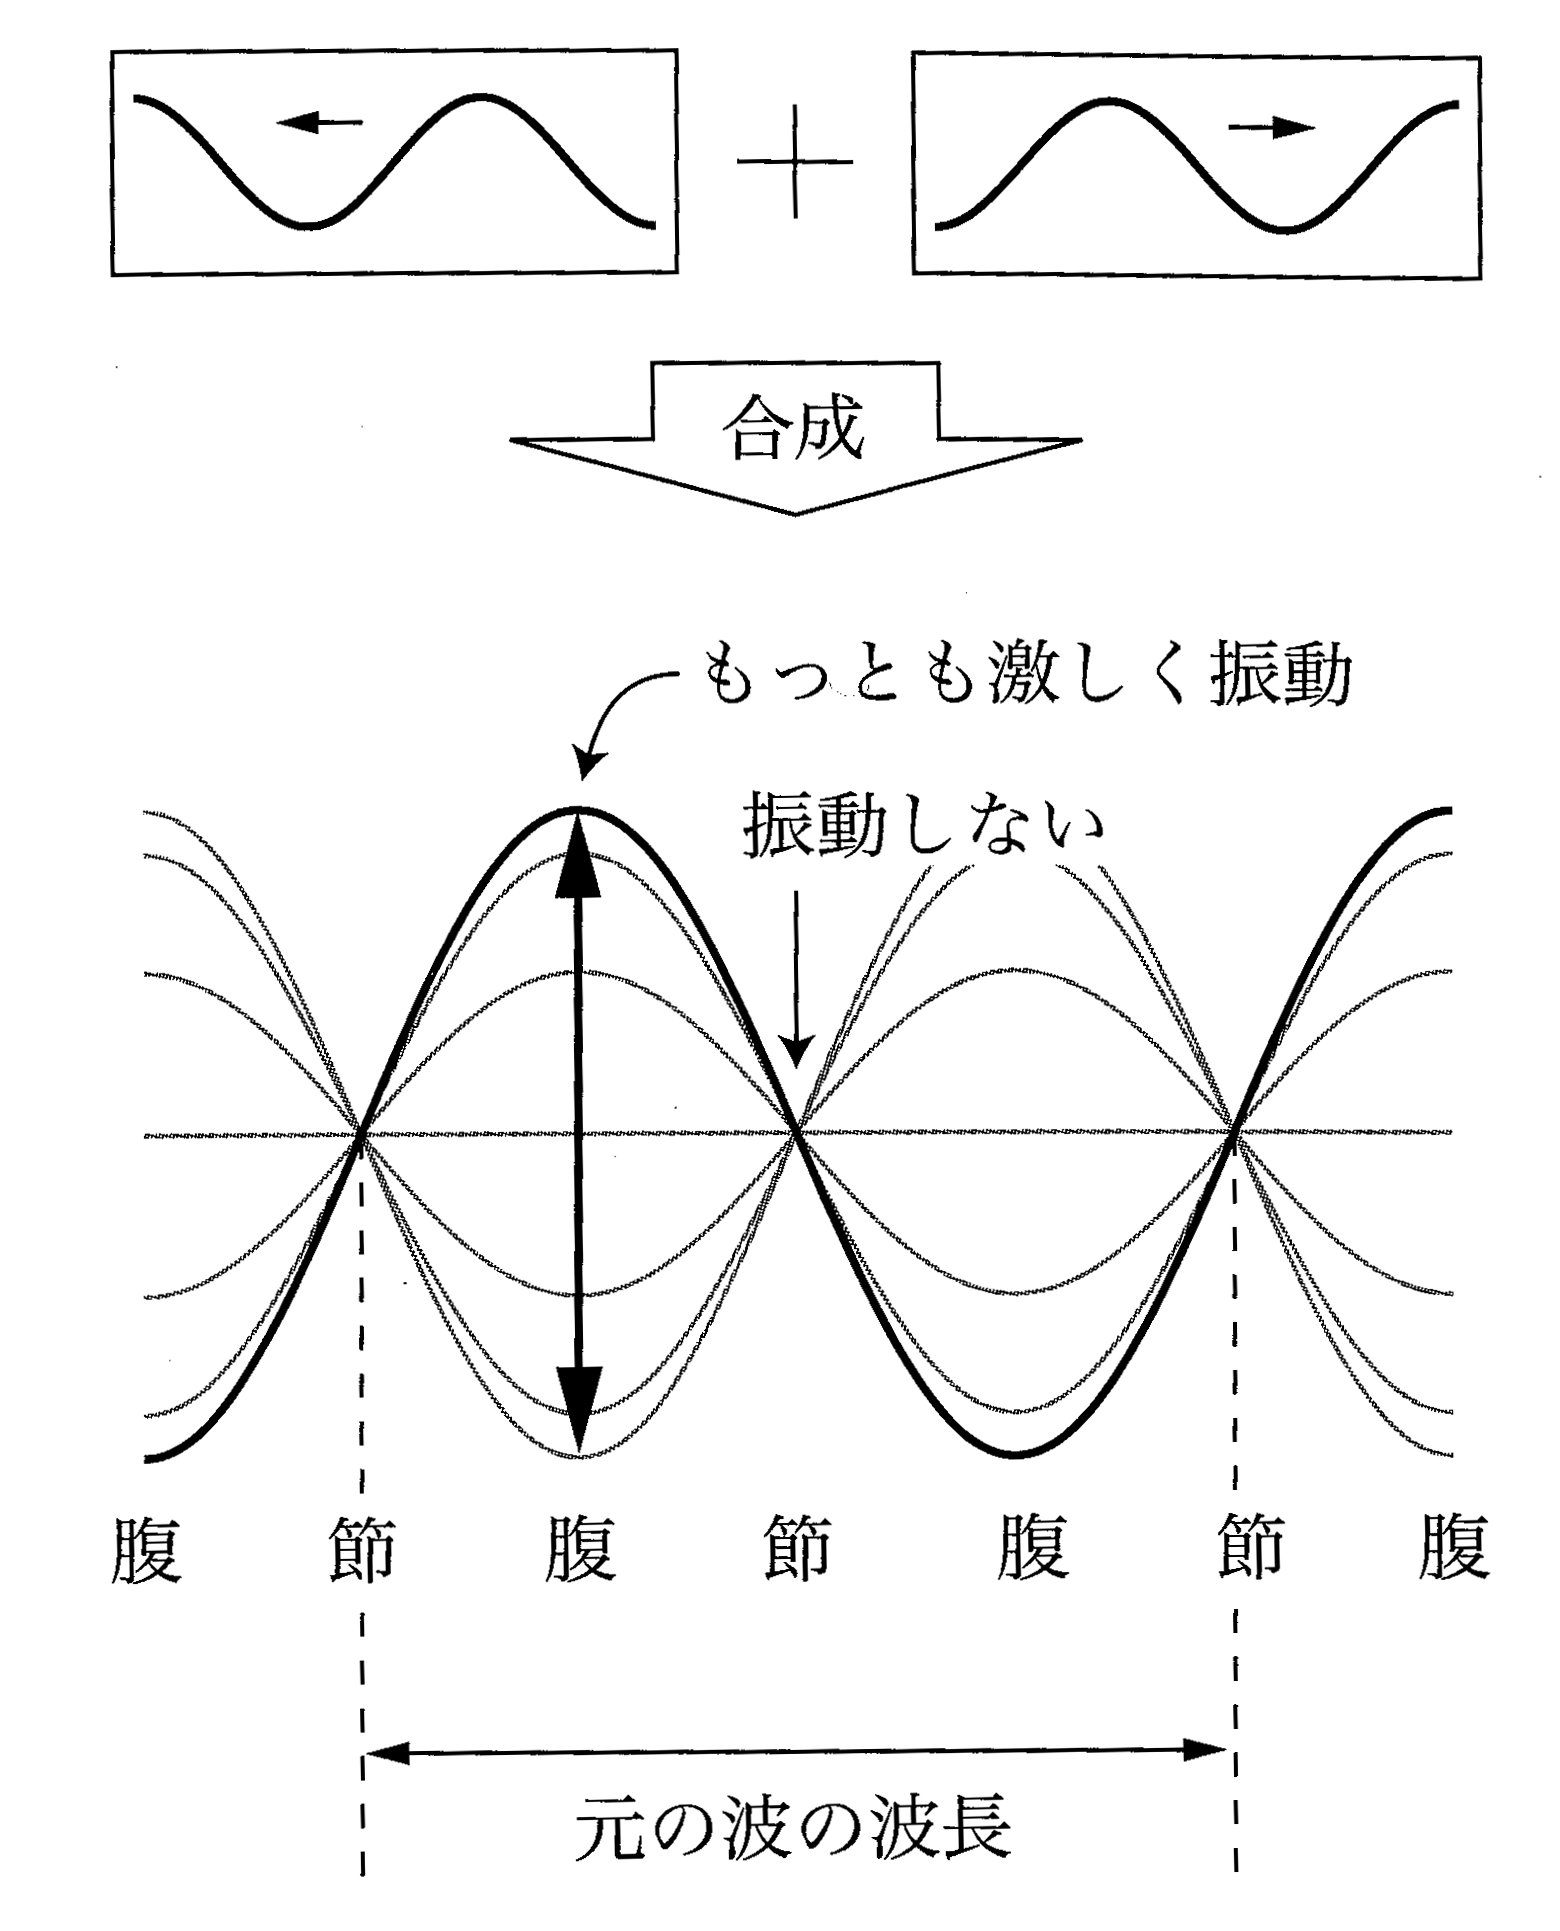
\includegraphics[keepaspectratio,width=70mm]
  {text_p95_fig1.png}
\end{wrapfigure}
先の水面波の干渉では，水面上に節線，・腹線ができたが，特に2つの波源を結ぶ線分上では波形がどちら方向にも進行しない波が観察される．
一般に，{\bf 一直線上で，互いに逆向きに伝播する，波長・振幅・振動数の等しい2つの波が重なった場合，大きく振動する点と，全く振動しない点とが交互に並び，それらの点がそれらの点が左右どちらにも動かない波が観察される．}
このような波を{\bf 定常波（または定在波）}と呼ぶ．

右図は合成波の様子を表したものであるが，場所により最大の変位（振幅）は異なり，最も大きく振動する点を腹，全く振動しない点を節という．
右図のもとの波長と比較すれば，{\bf 腹と腹の間隔，節と節の間隔は波長の半分の長さであり，腹と節の間隔は波長の}\mbox{\boldmath $\dfrac{1}{4}$}となることがわかる．
また，定常波の周期はもとの波の周期と一致している．

\vspace{15mm}
\begin{matome}{定常波}
 \hspace{3mm} 互いに逆方向に進む同一振幅・波長・周期の2つの波が重なるとき，合成波は進行しない定常波となる．
 振幅は媒質各点ごとに違い，各点で上下に単振動を行うが，波形は左右には動いていかない．
 \[ 定常波の腹-腹間隔＝節-節間隔＝\dfrac{\lambda}{2} \hspace{10mm} 腹-節間隔＝\dfrac{\lambda}{4}\]
\end{matome}

\subsection{うなり}
\begin{wrapfigure}[9]{r}[5mm]{50mm}
  \centering
  \vspace{-10mm}
  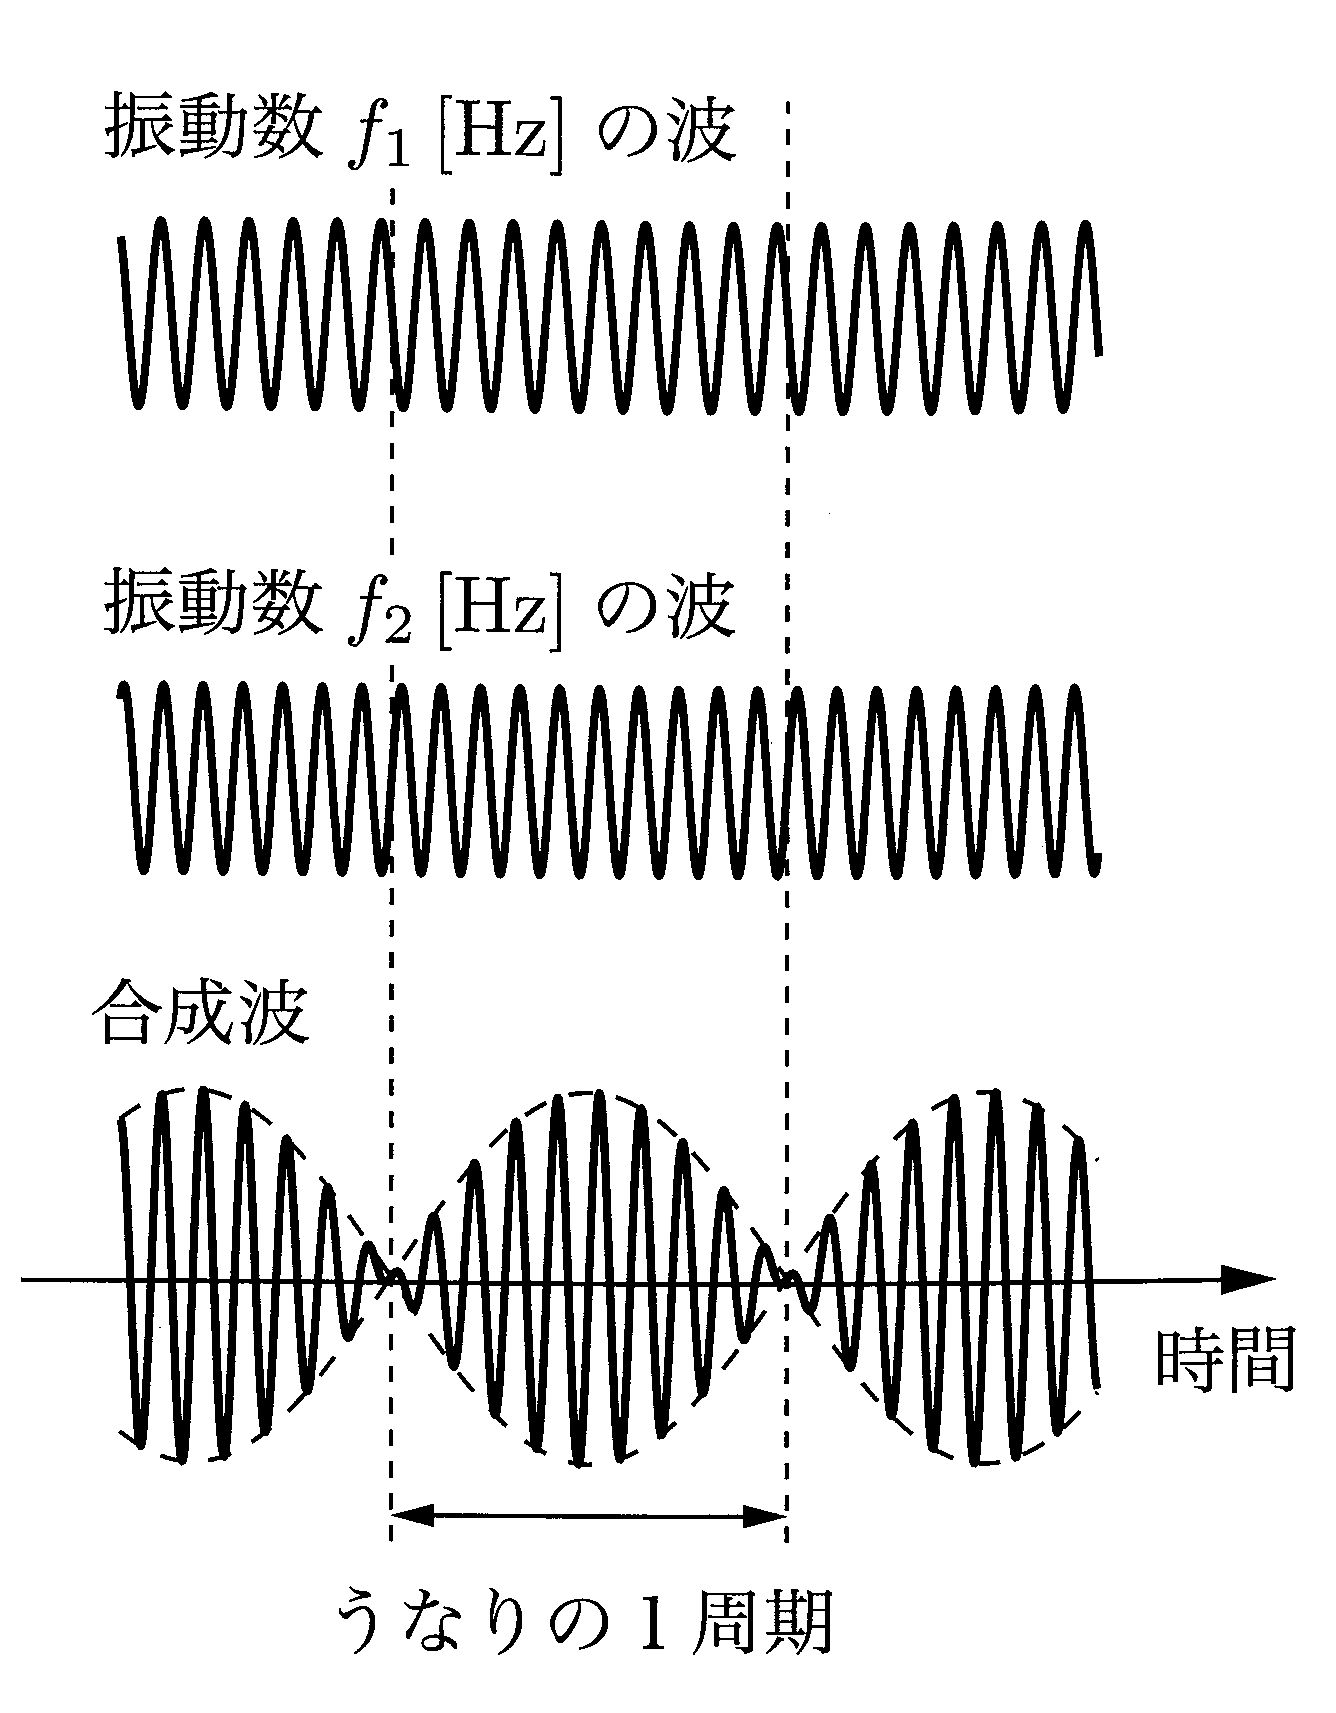
\includegraphics[keepaspectratio,width=50mm]
  {text_p96_fig1.png}
\end{wrapfigure}
定常波では同一振動数をもつ2つの波の干渉を考えたが，振動数がわずかに異なる2つの波の干渉では，合成波は図のように振幅の大きい部分と小さい部分を持つ波群となって伝播していく．
特に干渉する波が音波の場合は振幅は音の強さに対応するため，観測者は位置に関係なく，音が周期的に大きくなったり小さくなったりする現象を観測する．
この現象をうなりという．

うなりの振動数（1秒間あたりのうなりの回数）$N$[Hz]は，二つの波の振動数をそれぞれ$f_1,f_2$[Hz]として，
\[\mbox{\boldmath $N=|f_1-f_2|$} \hspace{2mm}[{\rm Hz}]\]
で与えられる．
\begin{matome}{うなり}
 \hspace{3mm} 振動数がそれぞれ$f_1,f_2$[Hz]の音波が干渉するとき，観測されるうなりの振動数$N$[Hz]は
\[N=|f_1-f_2| \hspace{2mm}[{\rm Hz}]\]
\end{matome}


\newpage

\begin{figure}[h]
\begin{center}
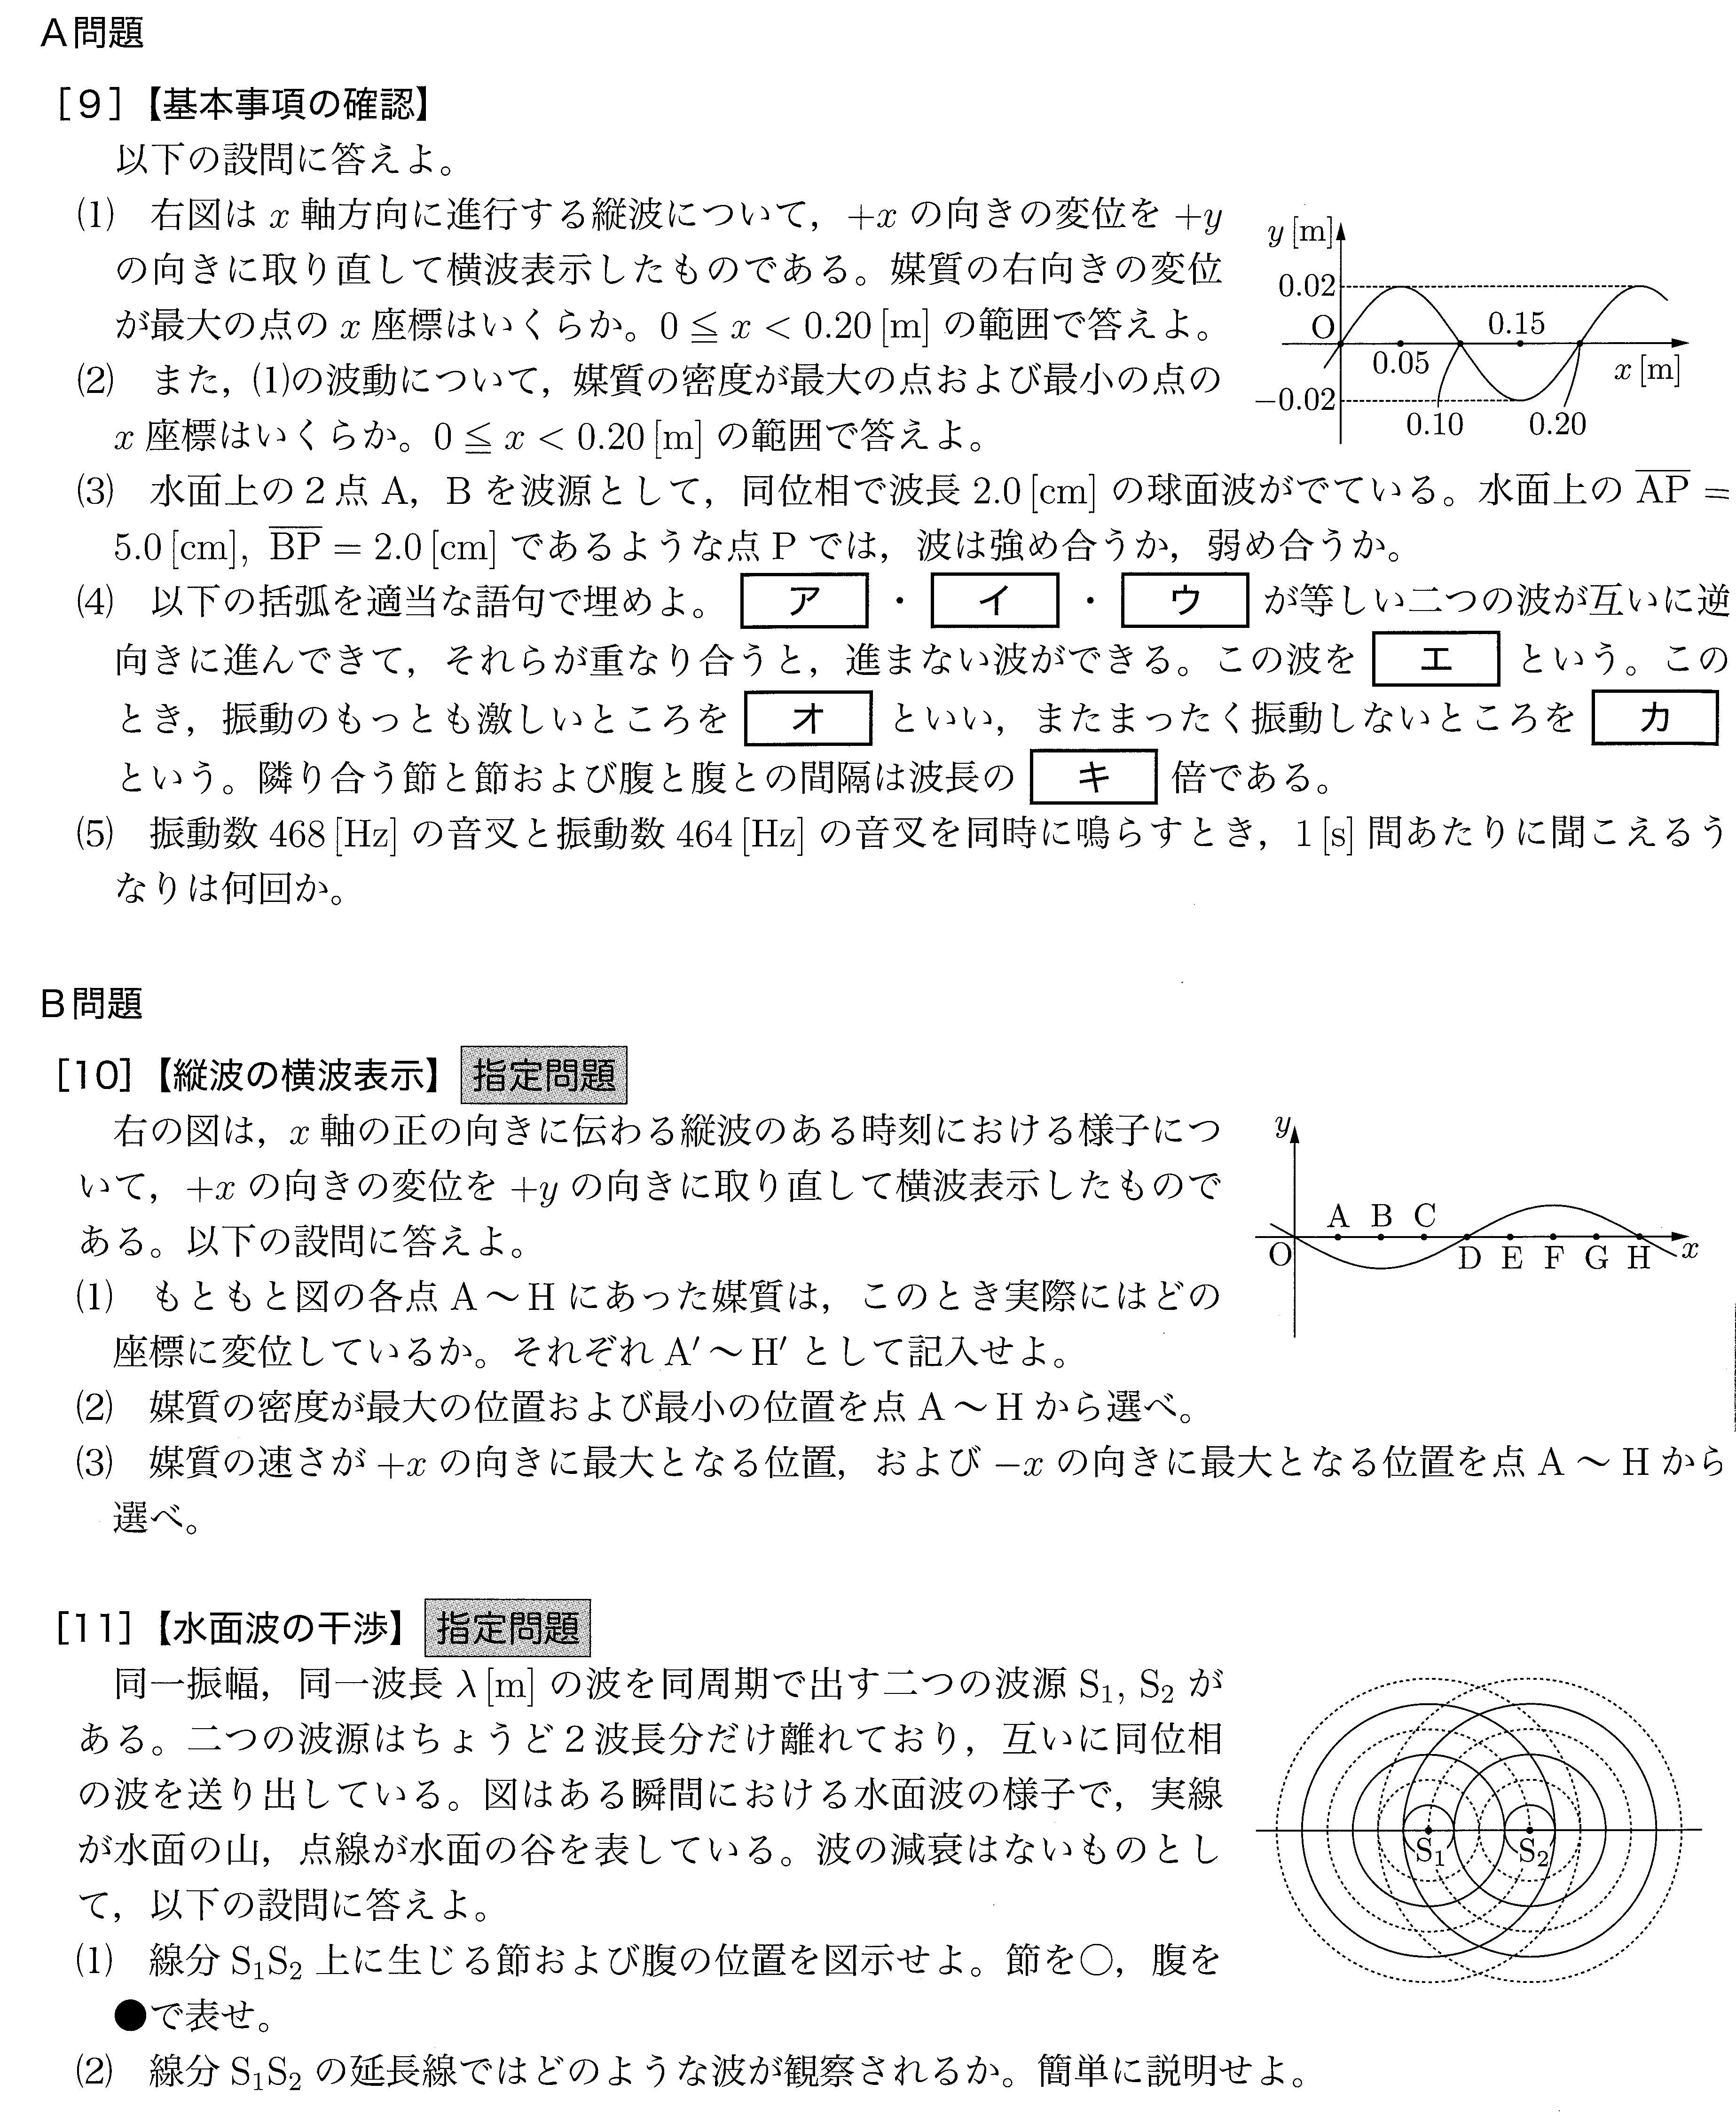
\includegraphics[width=170mm]{prob_p50.png}
\end{center}
\end{figure}
\newpage

\begin{figure}[h]
\begin{center}
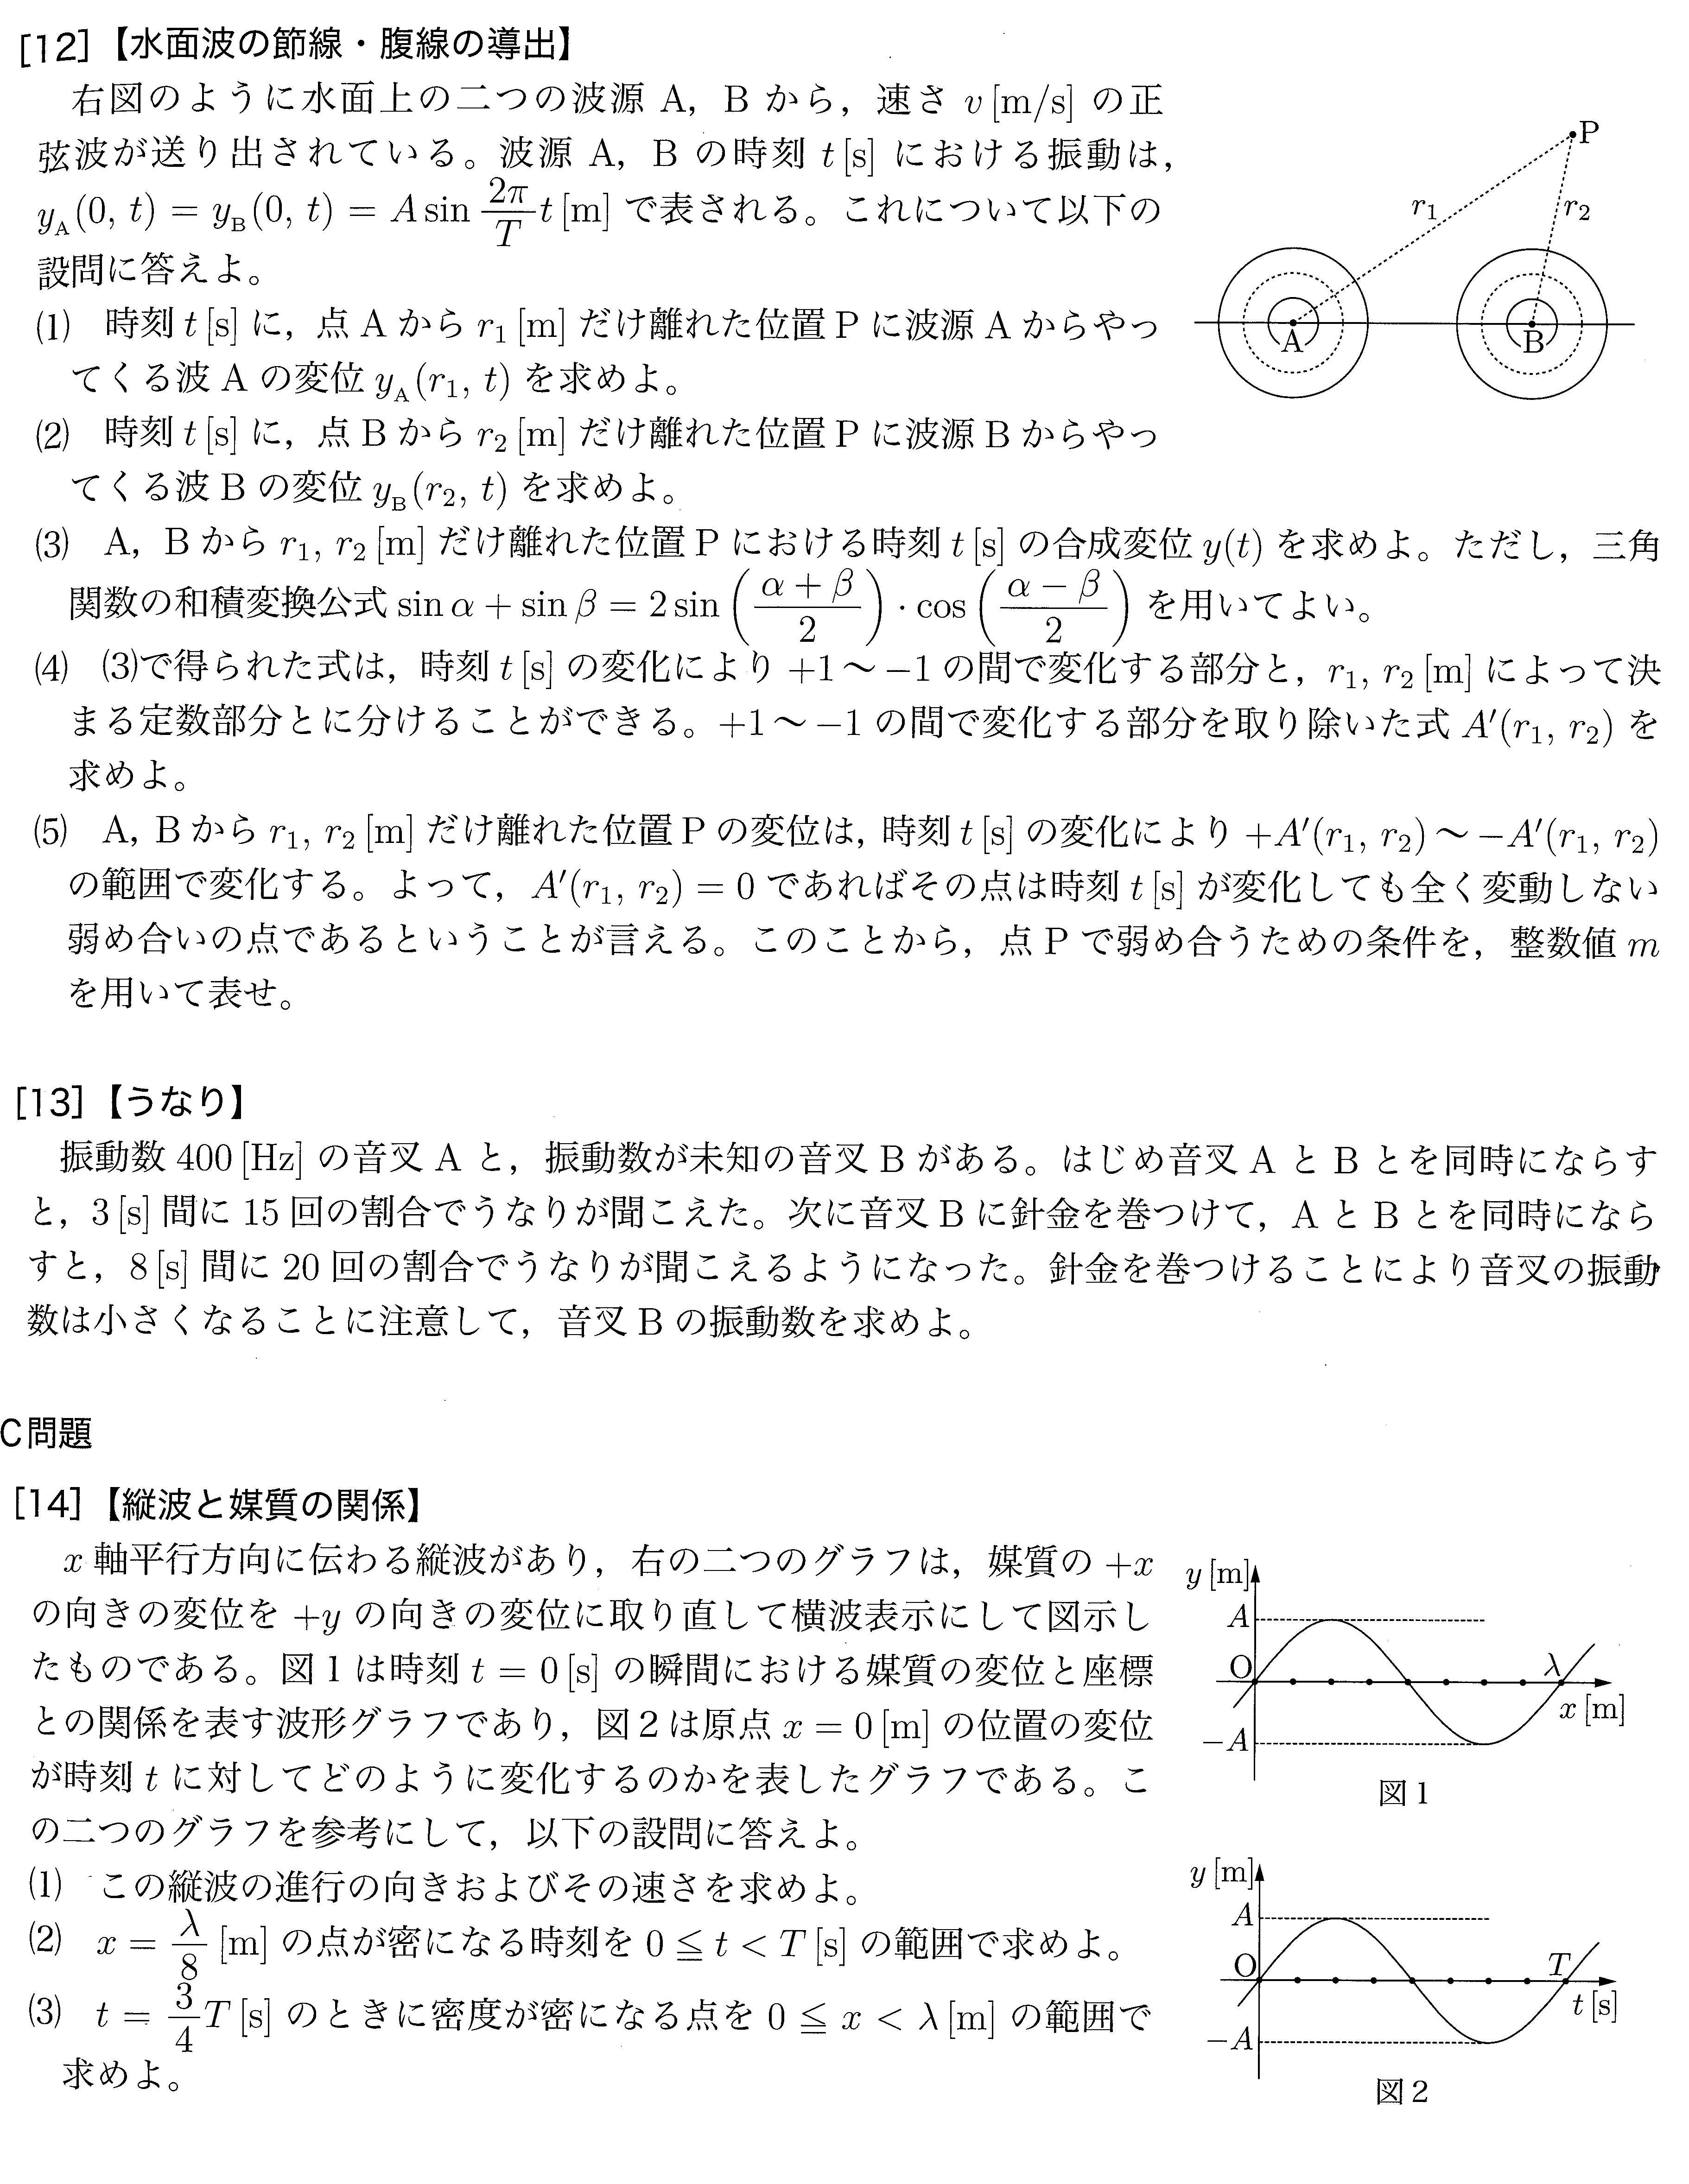
\includegraphics[width=170mm]{prob_p51.png}
\end{center}
\end{figure}
\newpage

\begin{figure}[h]
\begin{center}
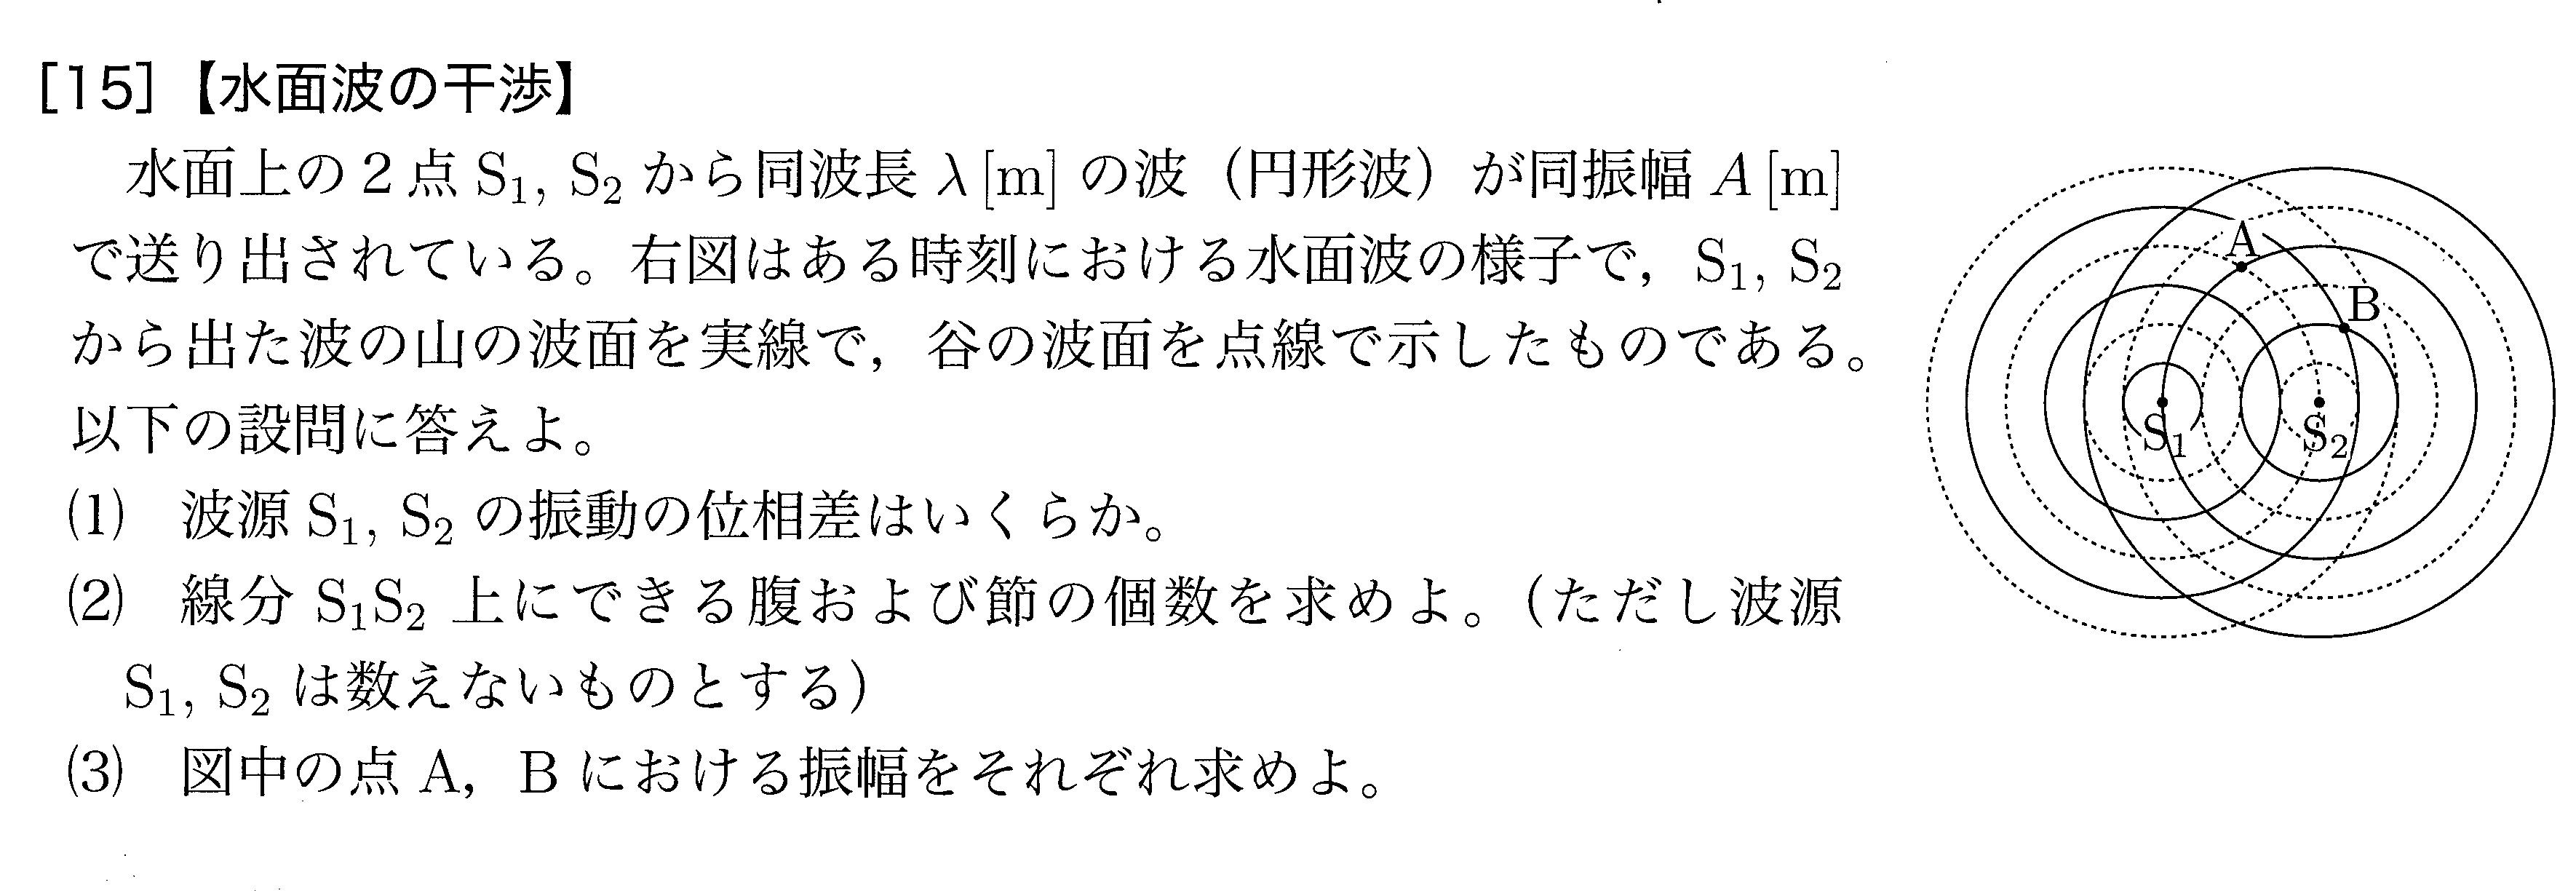
\includegraphics[width=170mm]{prob_p52.png}
\vspace{150mm}
\end{center}
\end{figure}


\newpage

\begin{figure}[h]
\begin{center}
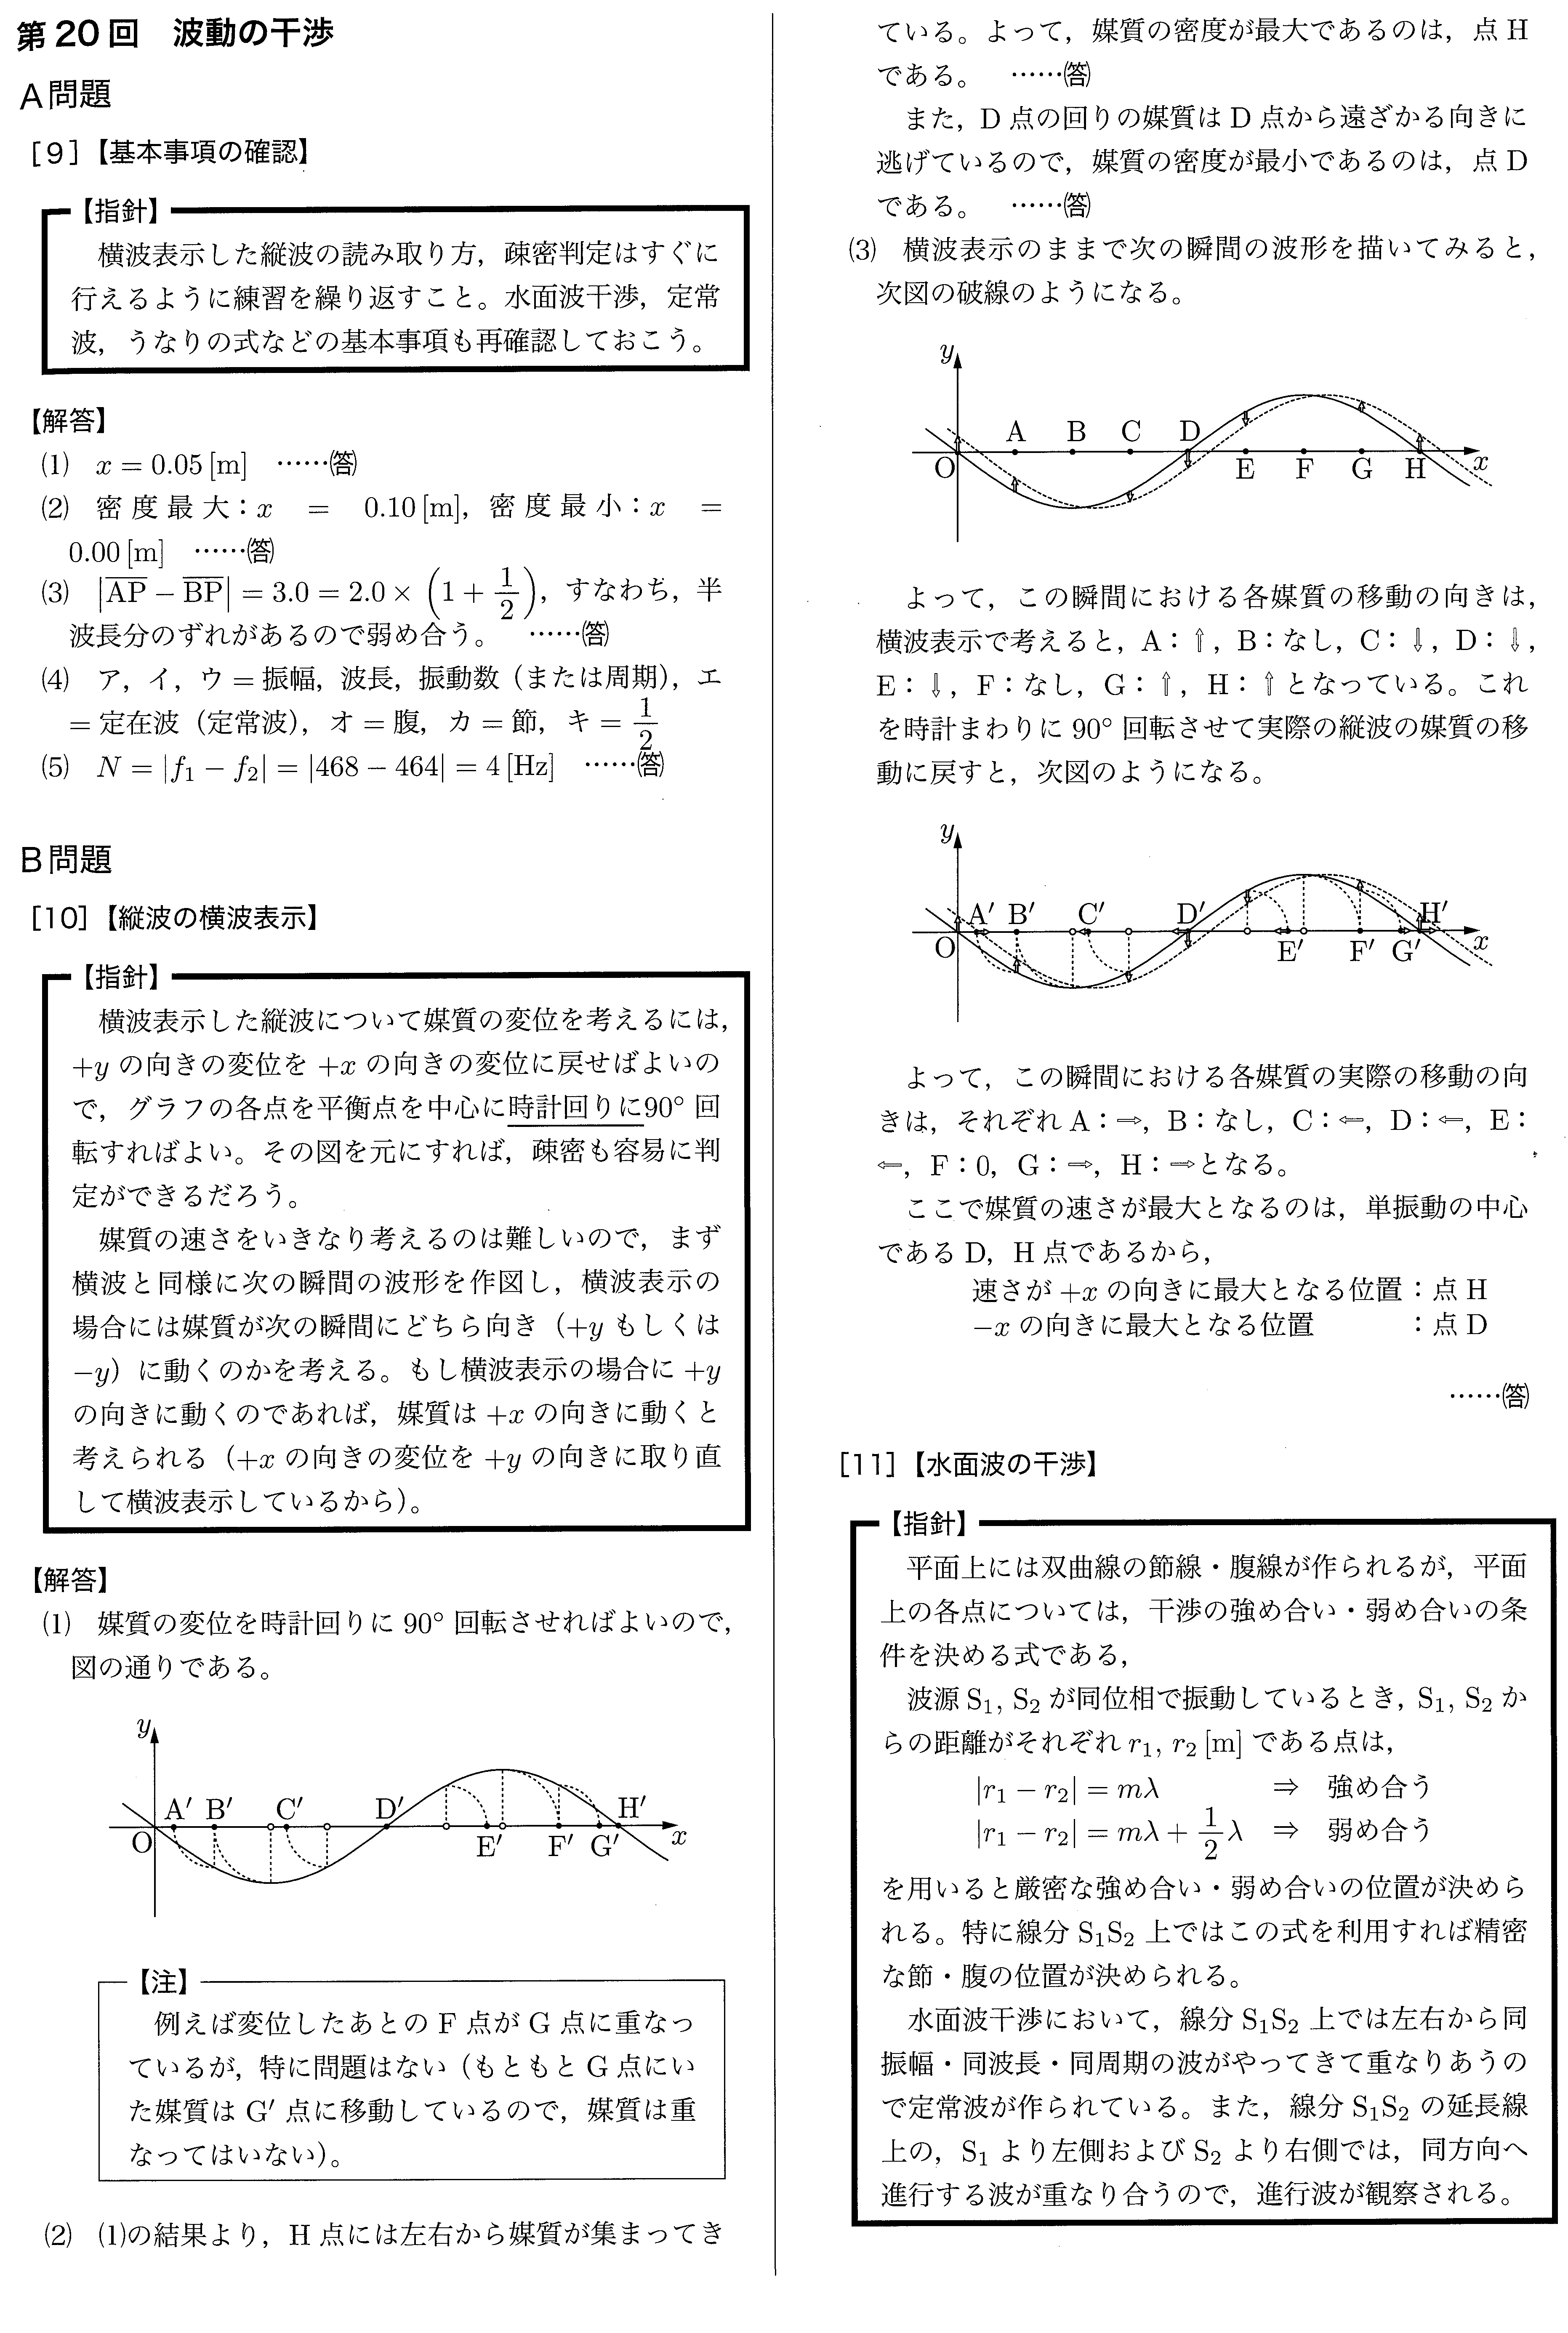
\includegraphics[width=170mm]{prob_p149.png}
\end{center}
\end{figure}
\newpage

\begin{figure}[h]
\begin{center}
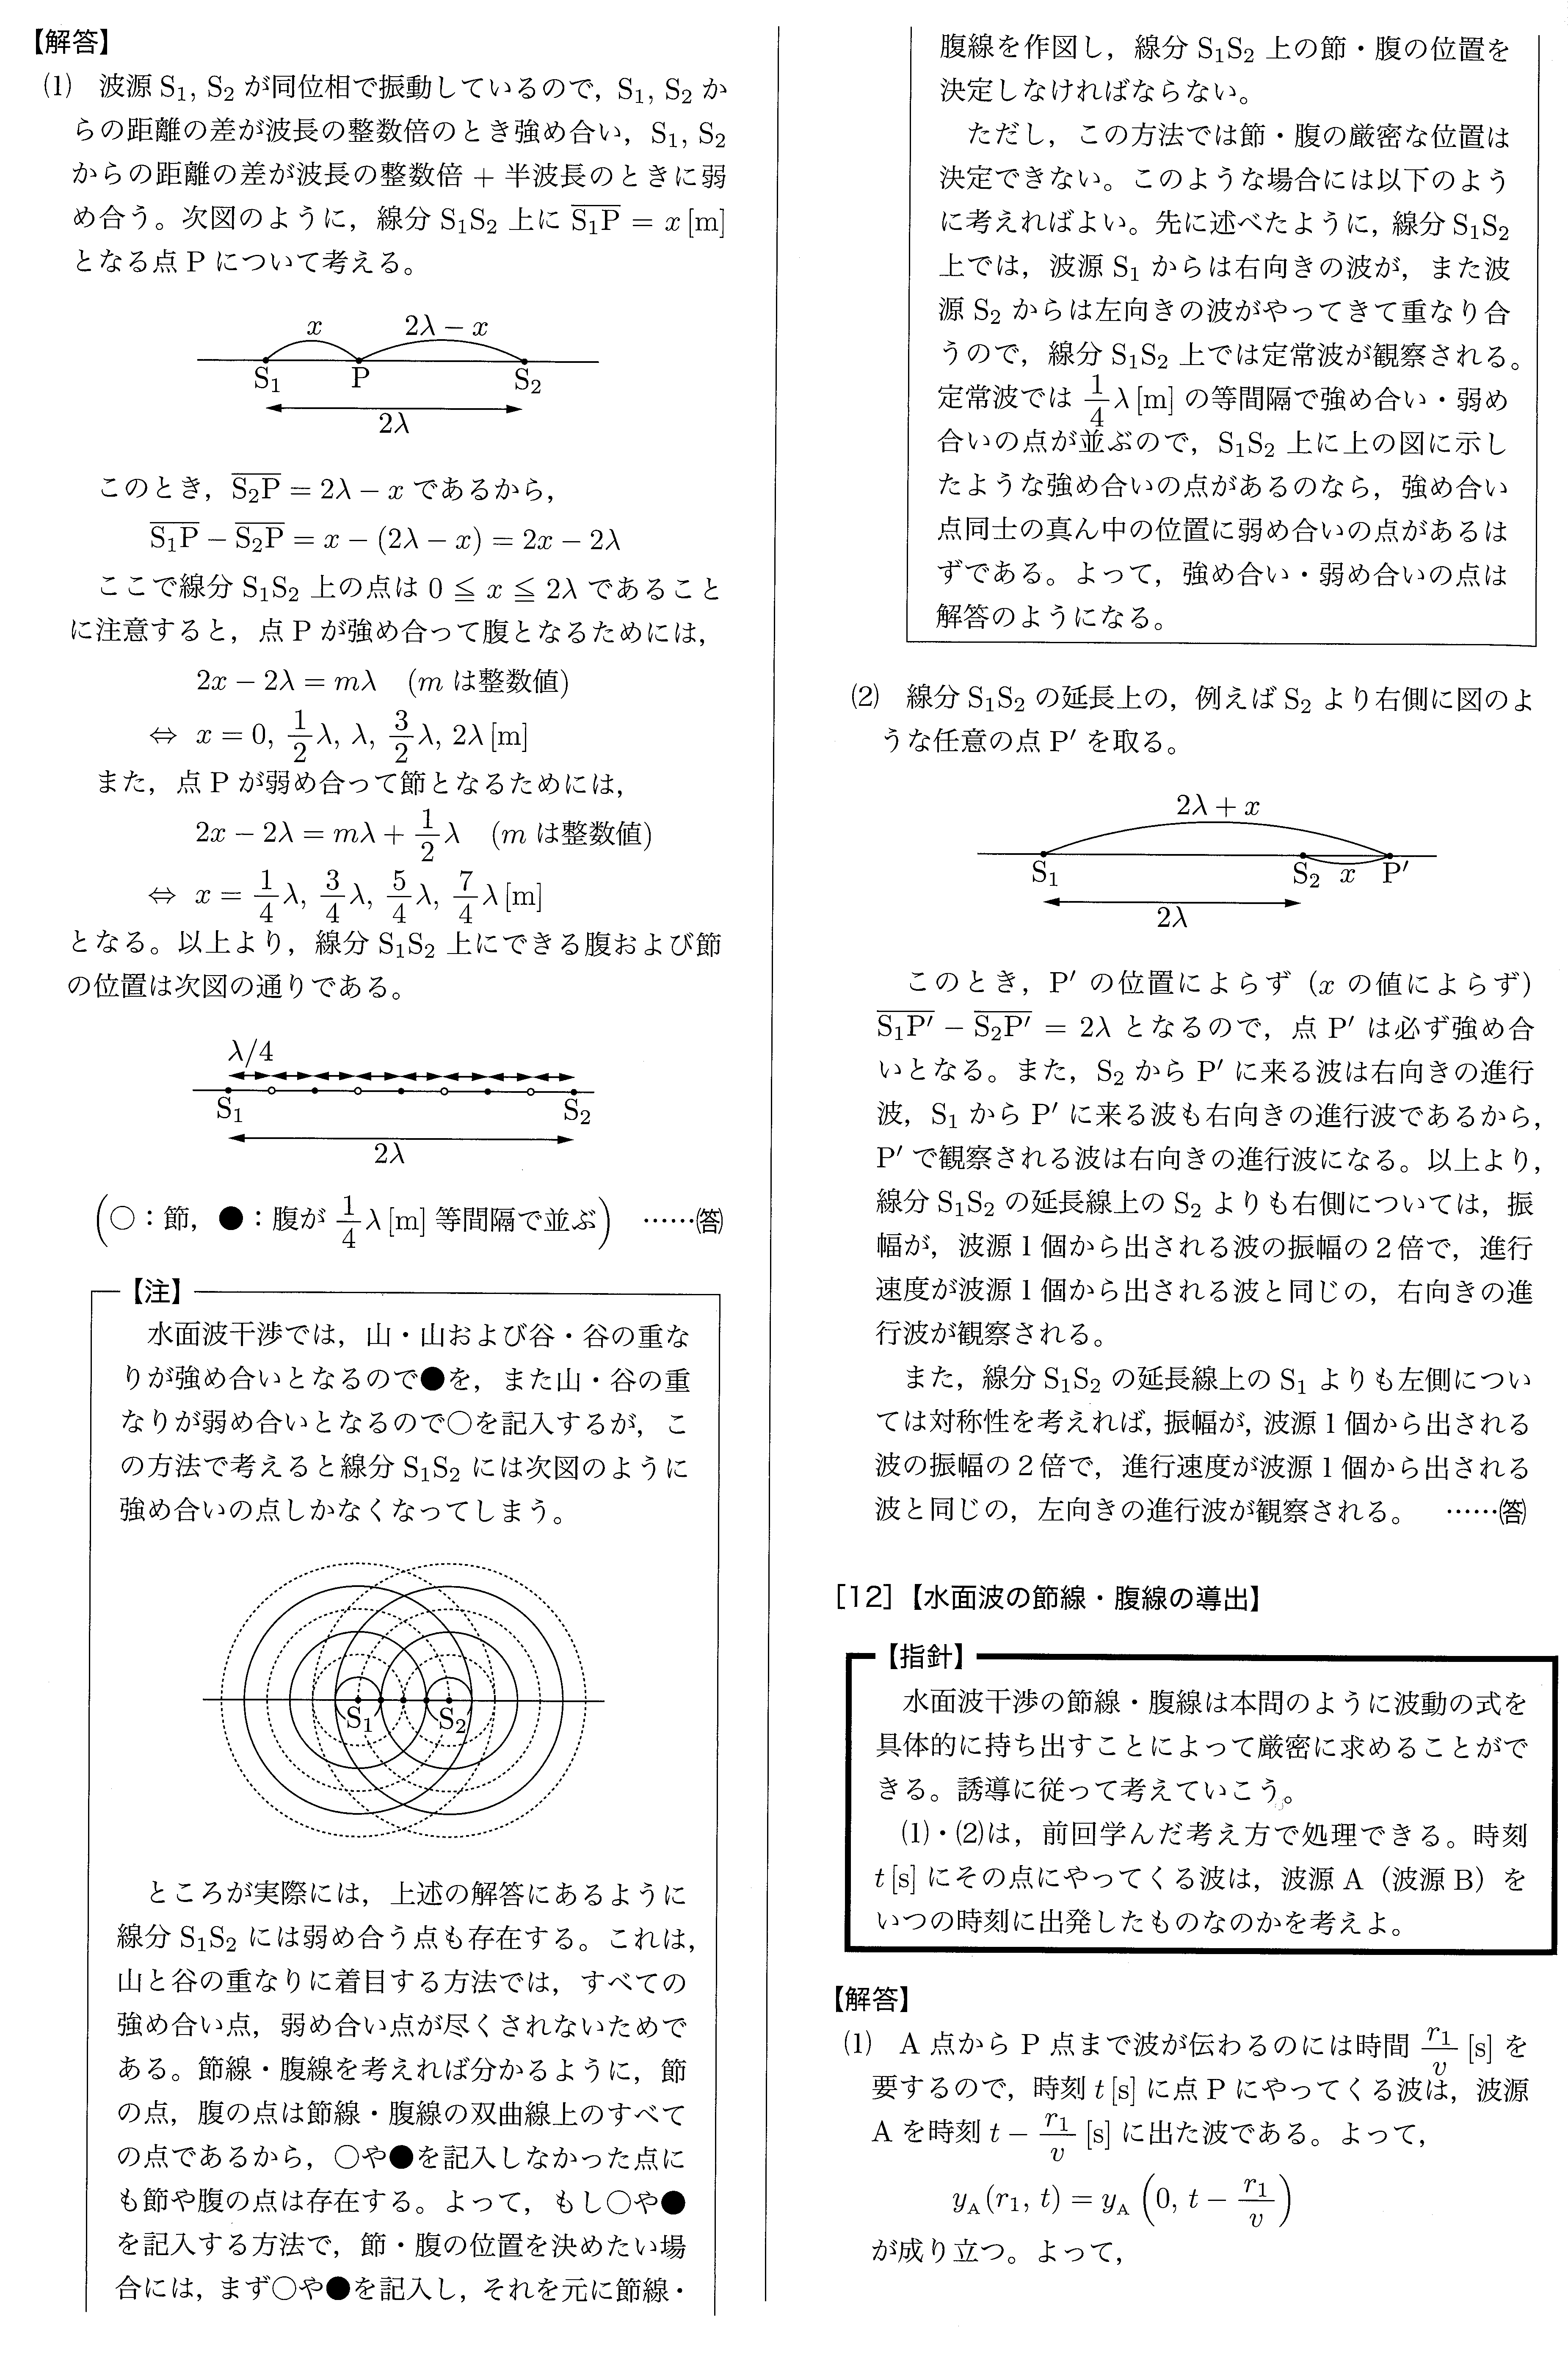
\includegraphics[width=170mm]{prob_p150.png}
\end{center}
\end{figure}
\newpage

\begin{figure}[h]
\begin{center}
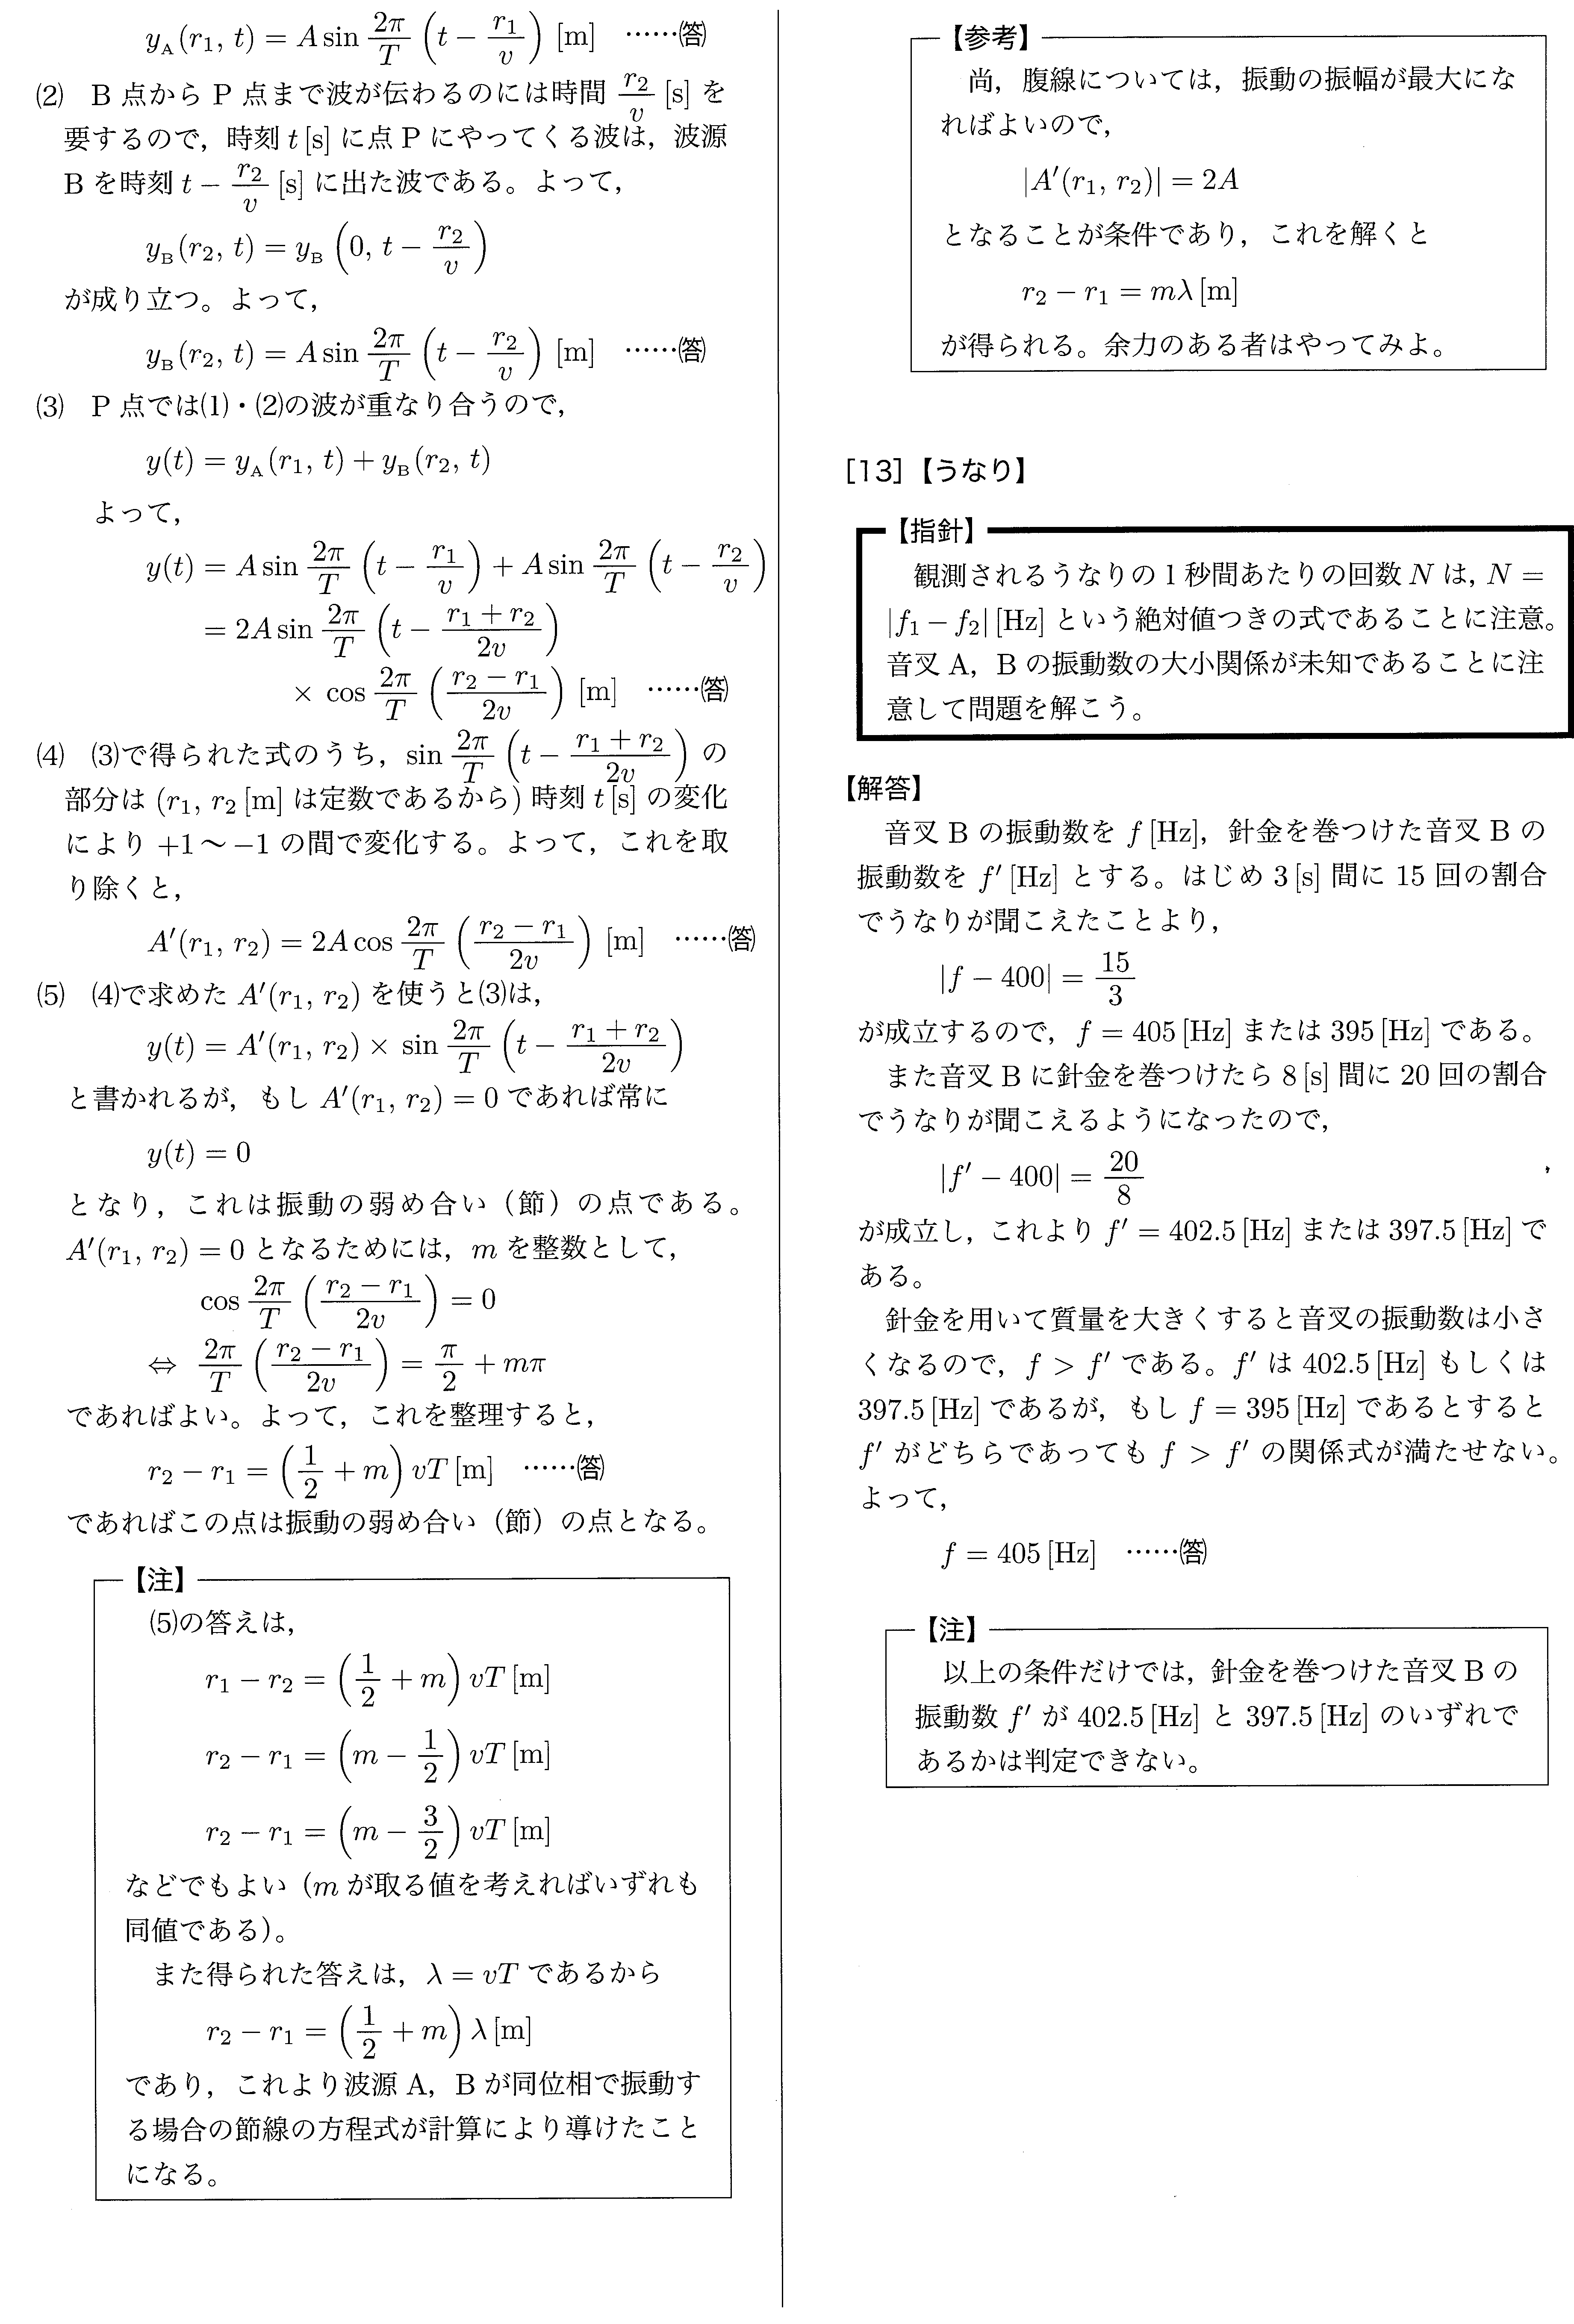
\includegraphics[width=170mm]{prob_p151.png}
\end{center}
\end{figure}

\newpage

\begin{figure}[h]
\begin{center}
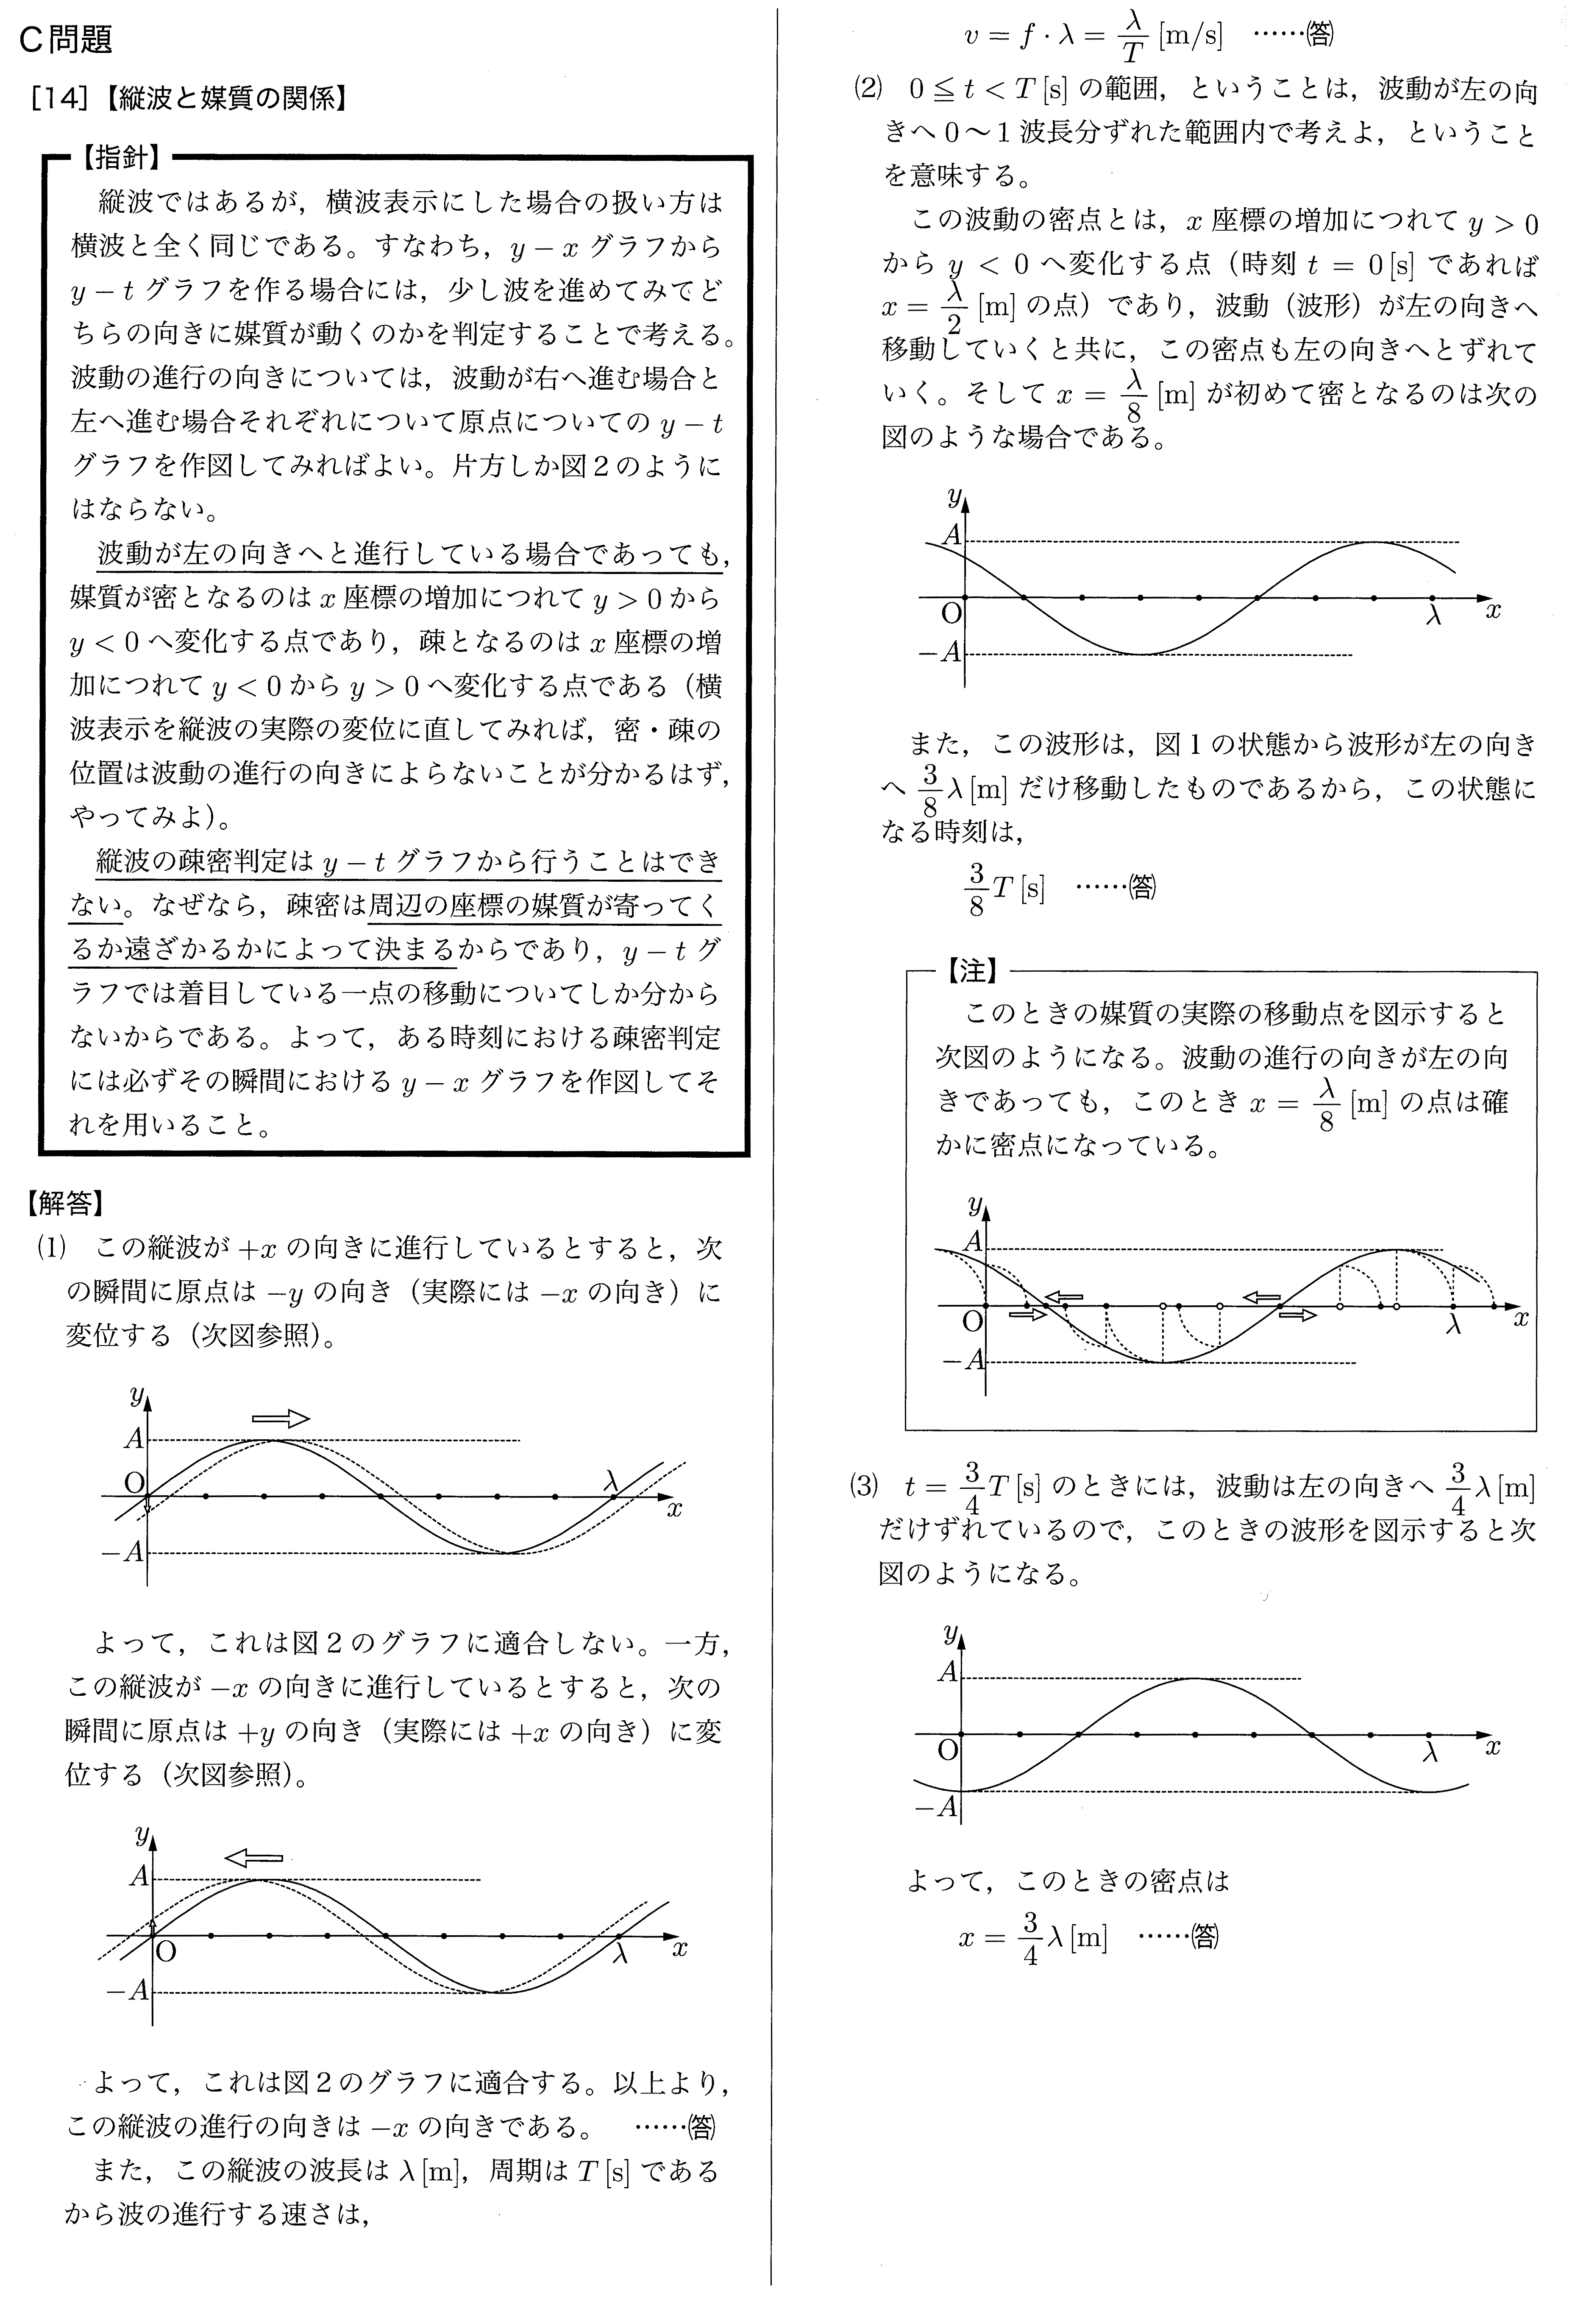
\includegraphics[width=170mm]{prob_p152.png}
\end{center}
\end{figure}
\newpage

\begin{figure}[h]
\begin{center}
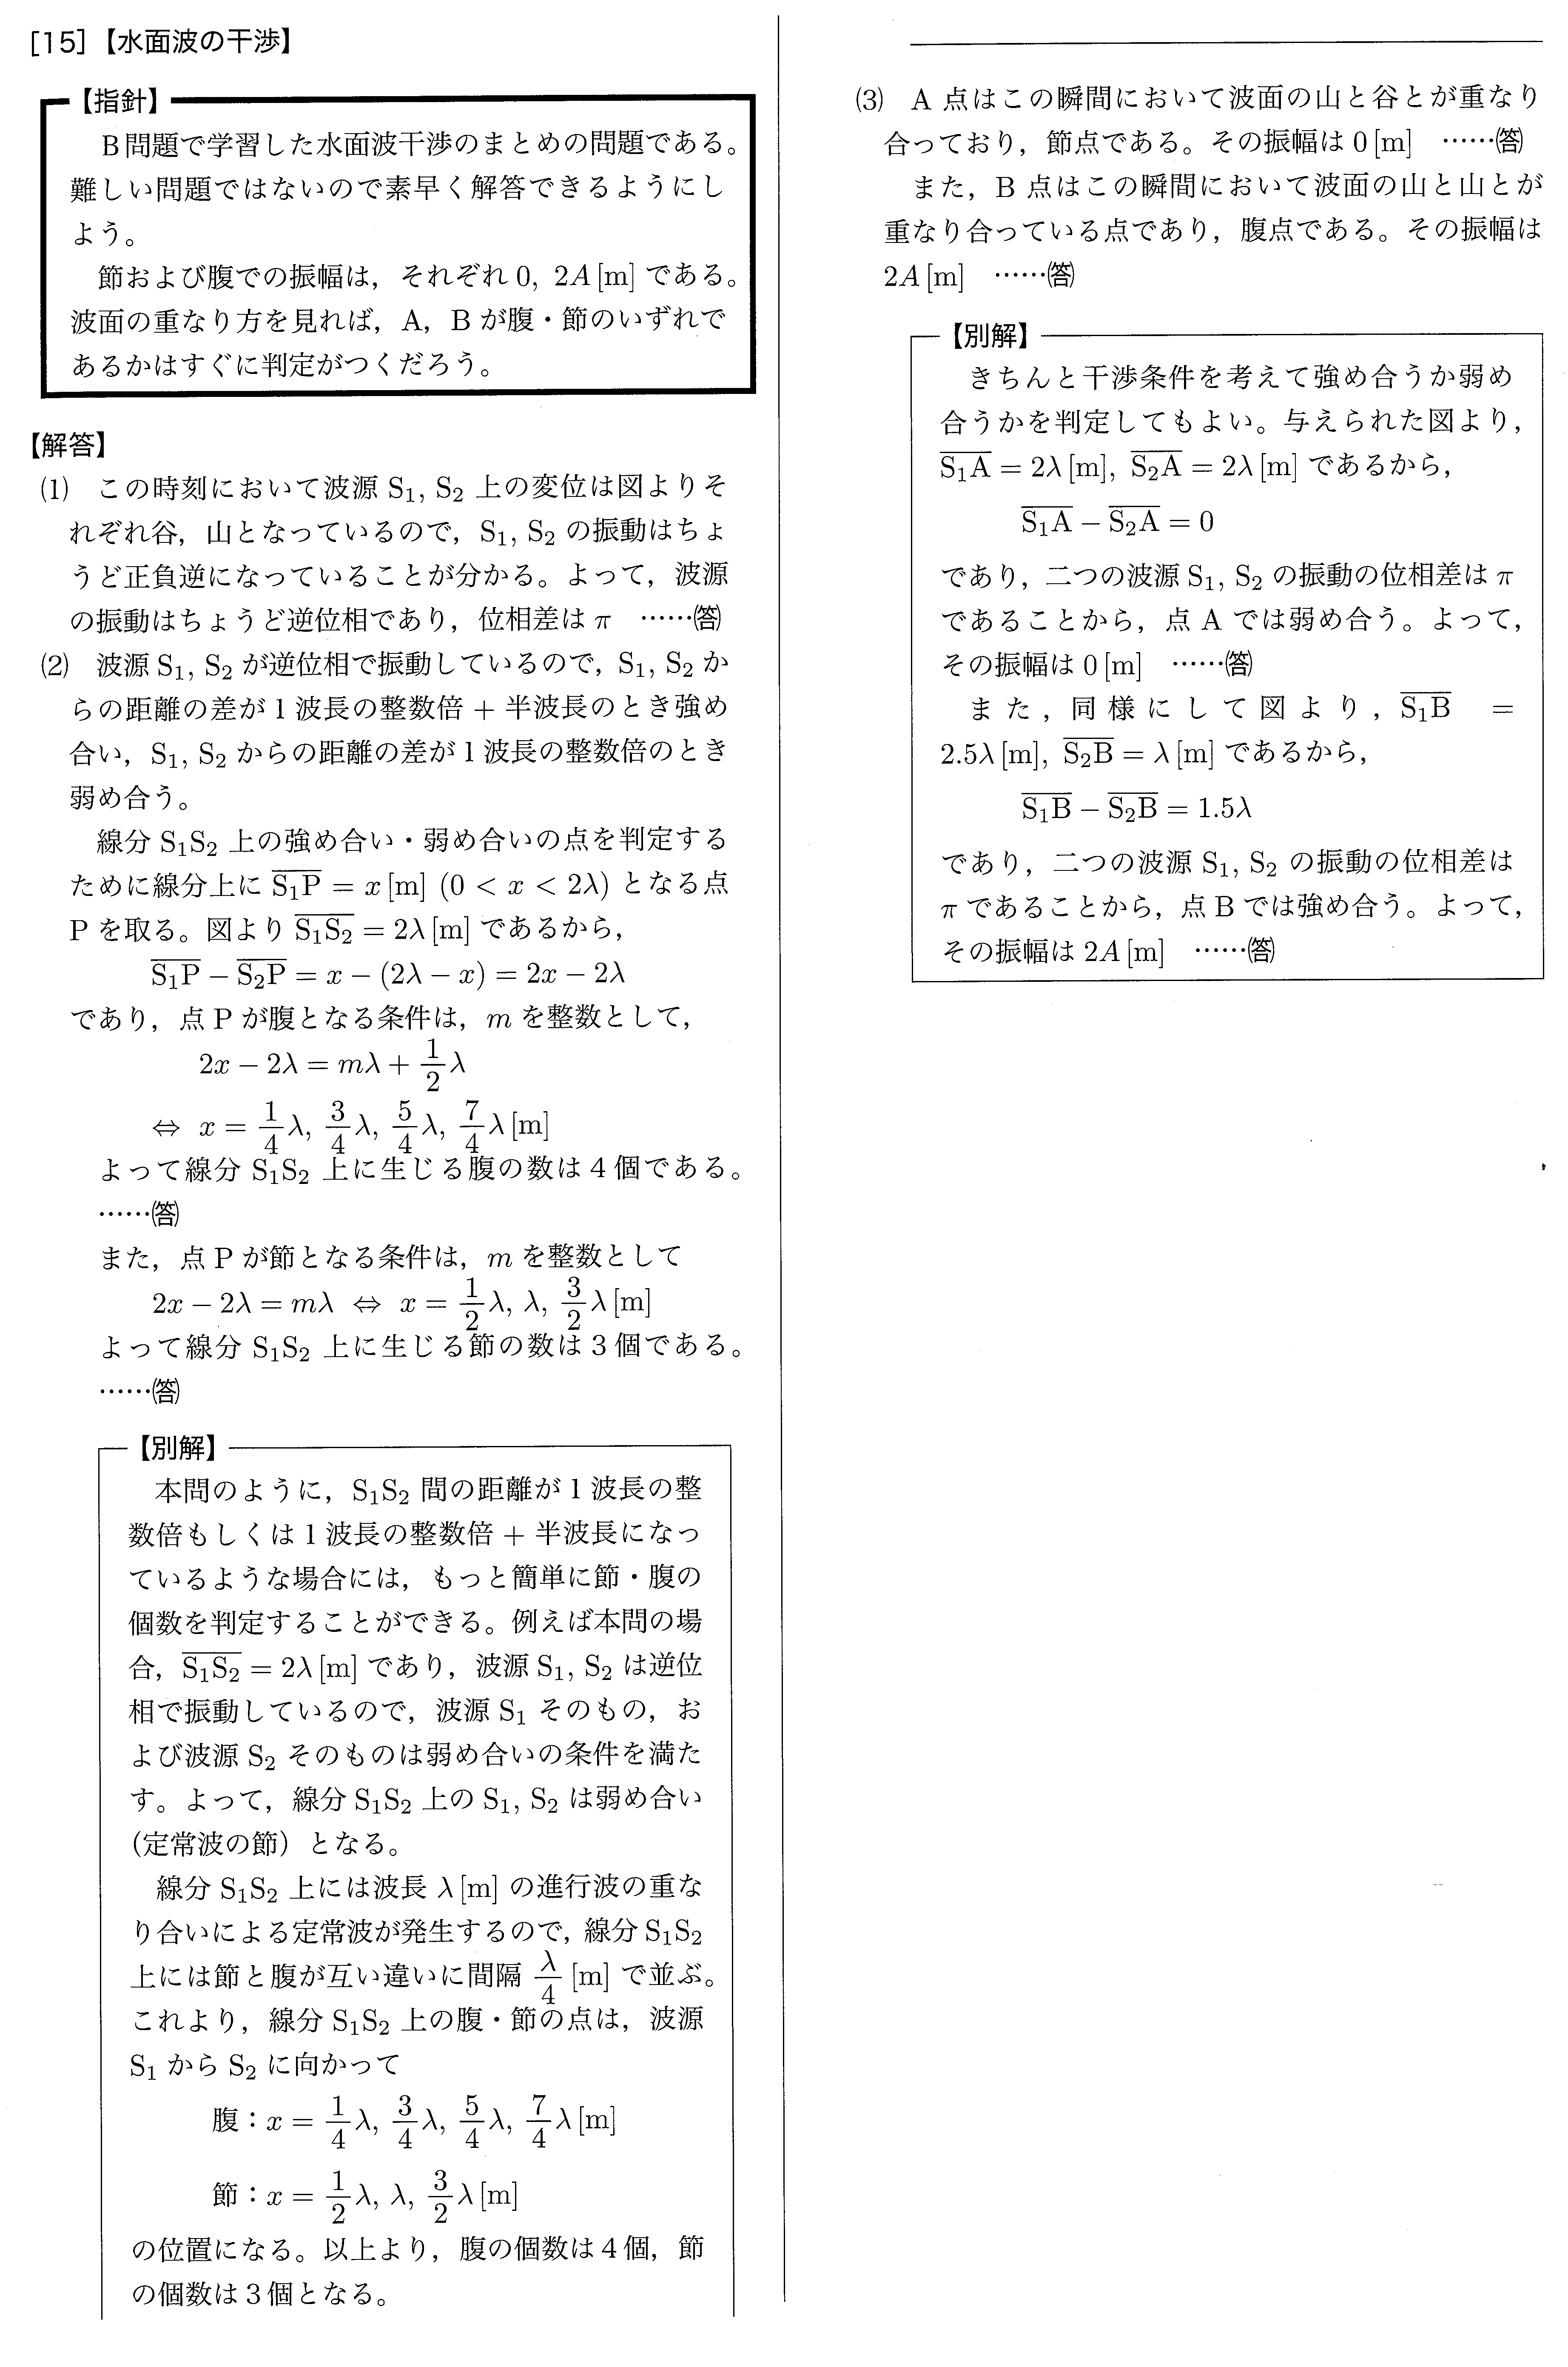
\includegraphics[width=170mm]{prob_p153.png}
\end{center}
\end{figure}
\section{自由端反射と固定端反射}

\subsection{自由端と固定端}
糸を張り，この左端を上下に振って波を送る場合，壁面に達した波は反射されて逆方向に戻ってくる．
この際，糸が壁面に固定されているか，それとも壁面に対して自由に動けるかで反射のされ方が異なる．
媒質が反射点に固定されていて動けない反射点を{\bf 固定端}といい，媒質が反射点に固定されておらず，自由に動ける反射点を{\bf 自由端}という．

一次元的に伝播する波で，入射した波が反射点ですべて反射される場合について考えてみよう．\\
\Kou{1}{自由端反射}

\begin{wrapfigure}[11]{r}[5mm]{80mm}
  \centering
 % \vspace{-5mm}
  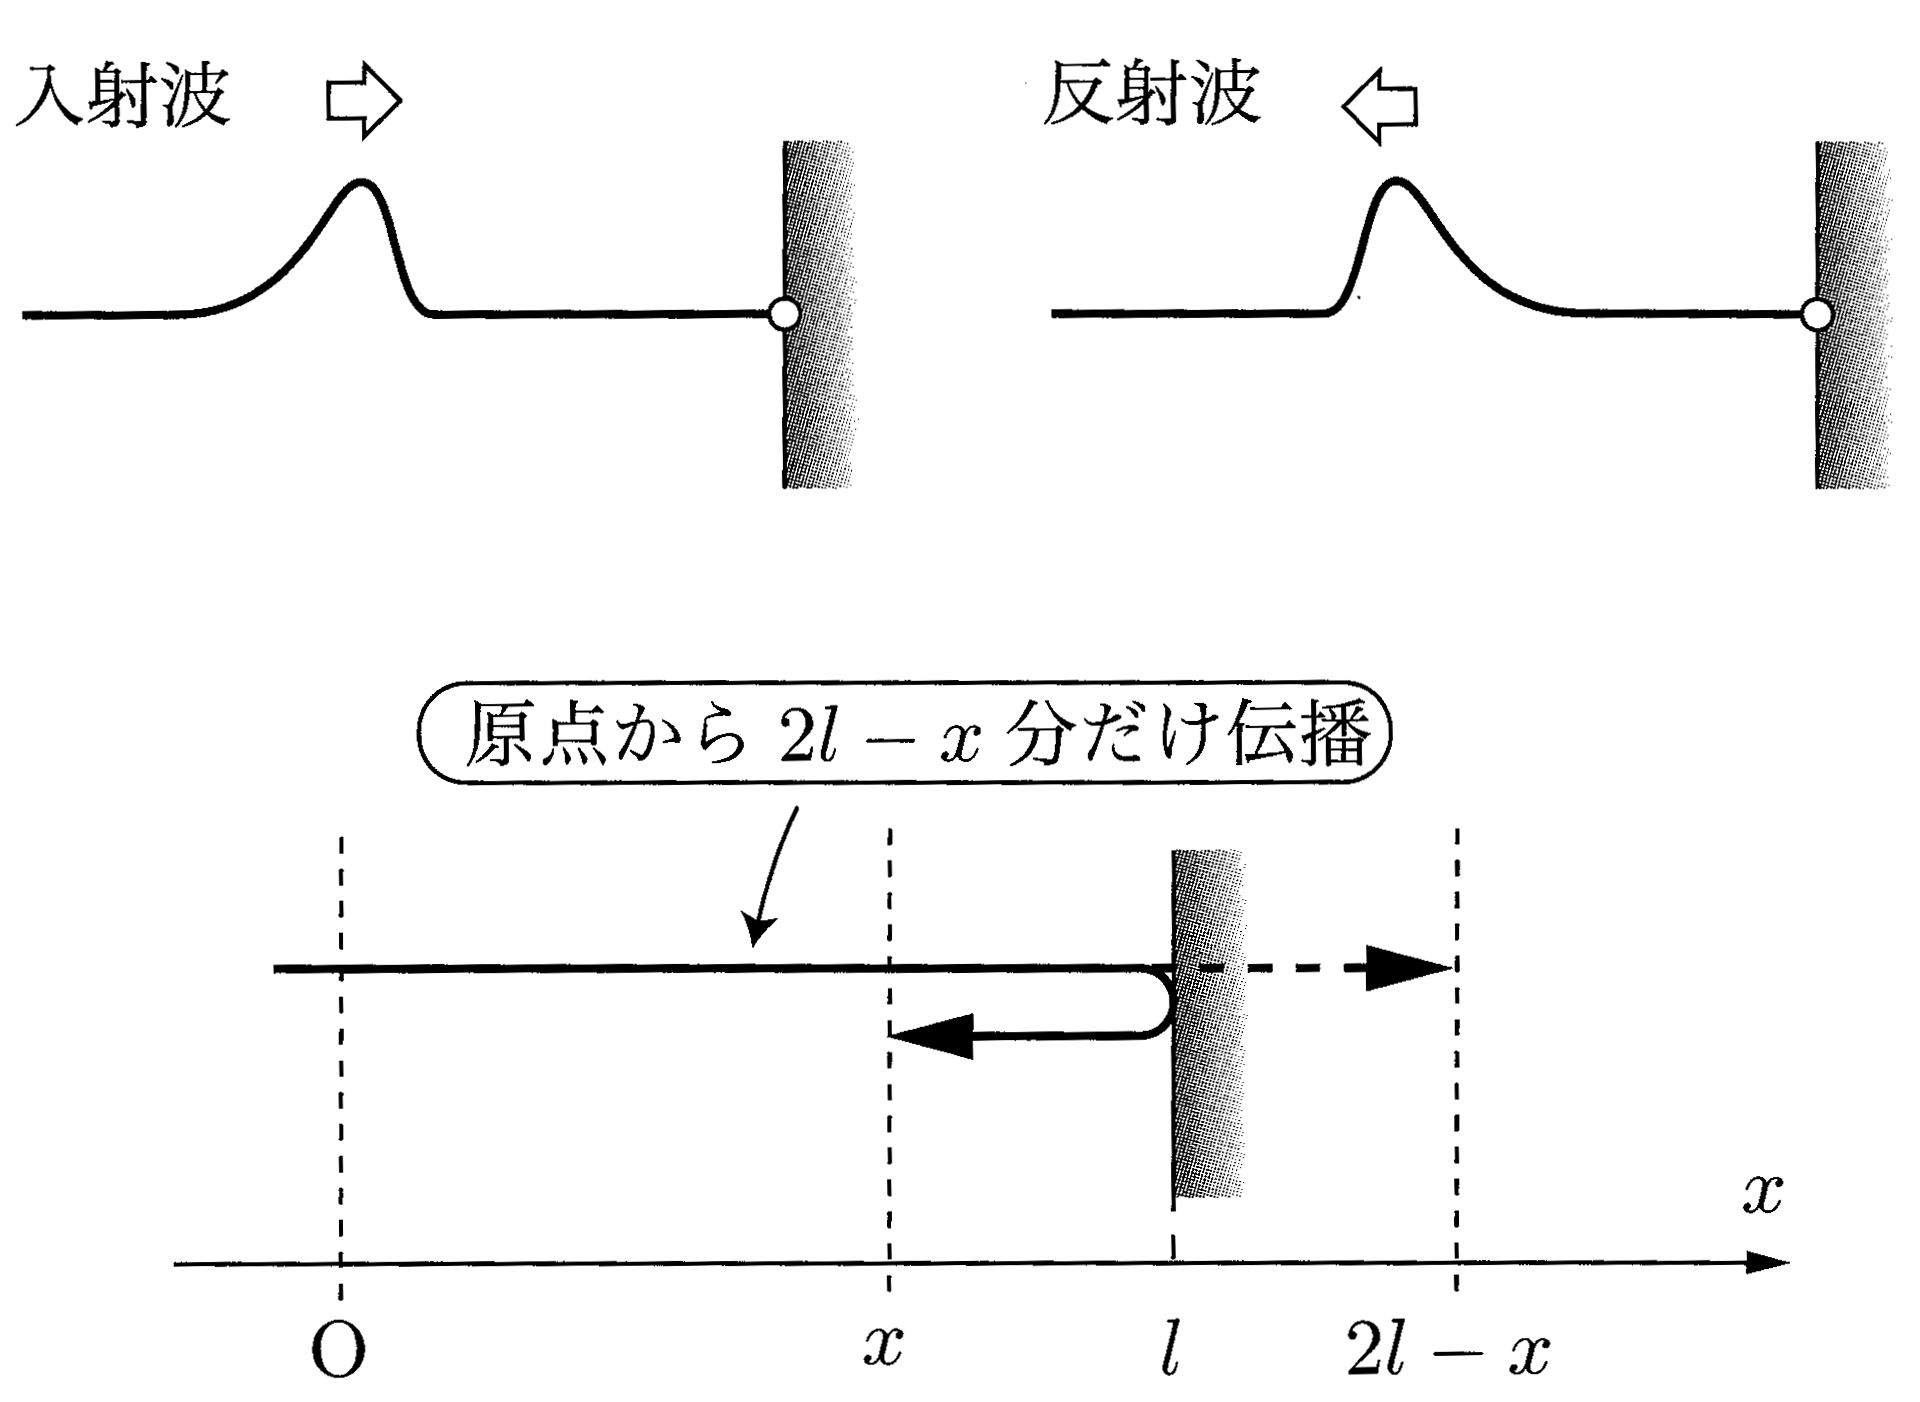
\includegraphics[keepaspectratio,width=80mm]
  {text_p97_fig1.png}
\end{wrapfigure}

 \mbox{\boldmath $反射点にある媒質が自由に動ける場合，自由端反射となる．$}
反射点において入射波と反射波の変位は同じになり，{\bf 反射波の波形は入射波を反射点で折り返した波形となる．}

図のように$x=l$[m]の位置に自由端反射する反射壁が置かれている場合，反射波の変位$y'(x,t)$[m]を考えてみよう．
波の伝播する速さを$v$[m/s]とし，原点での時刻$t$[s]での変位を$y(0,t)$[m]とすると，位置$x$[m]における反射波は原点から$2l-x$[m]だけ伝播してきたことになるので，この位置まで伝播するのに$\dfrac{2l-x}{v}$[s]だけ時間がかかるから
\[y'(x,t)=y\left( 0,t-\dfrac{2l-x}{v} \right) =y(2l-x,t)\]
と計算できる．
この変位は，入射波が反射壁で反射されずに$2l-x$[m]直進した場合の変位と等しく，このことは任意の位置，時刻で成立するから，{\bf 反射波の波形は入射波がそのまま直進した場合の波形を反射壁で折り返した波形と同じになる．}\\
\Kou{2}{固定端反射}

\begin{wrapfigure}[11]{r}[5mm]{80mm}
  \centering
%  \vspace{-5mm}
  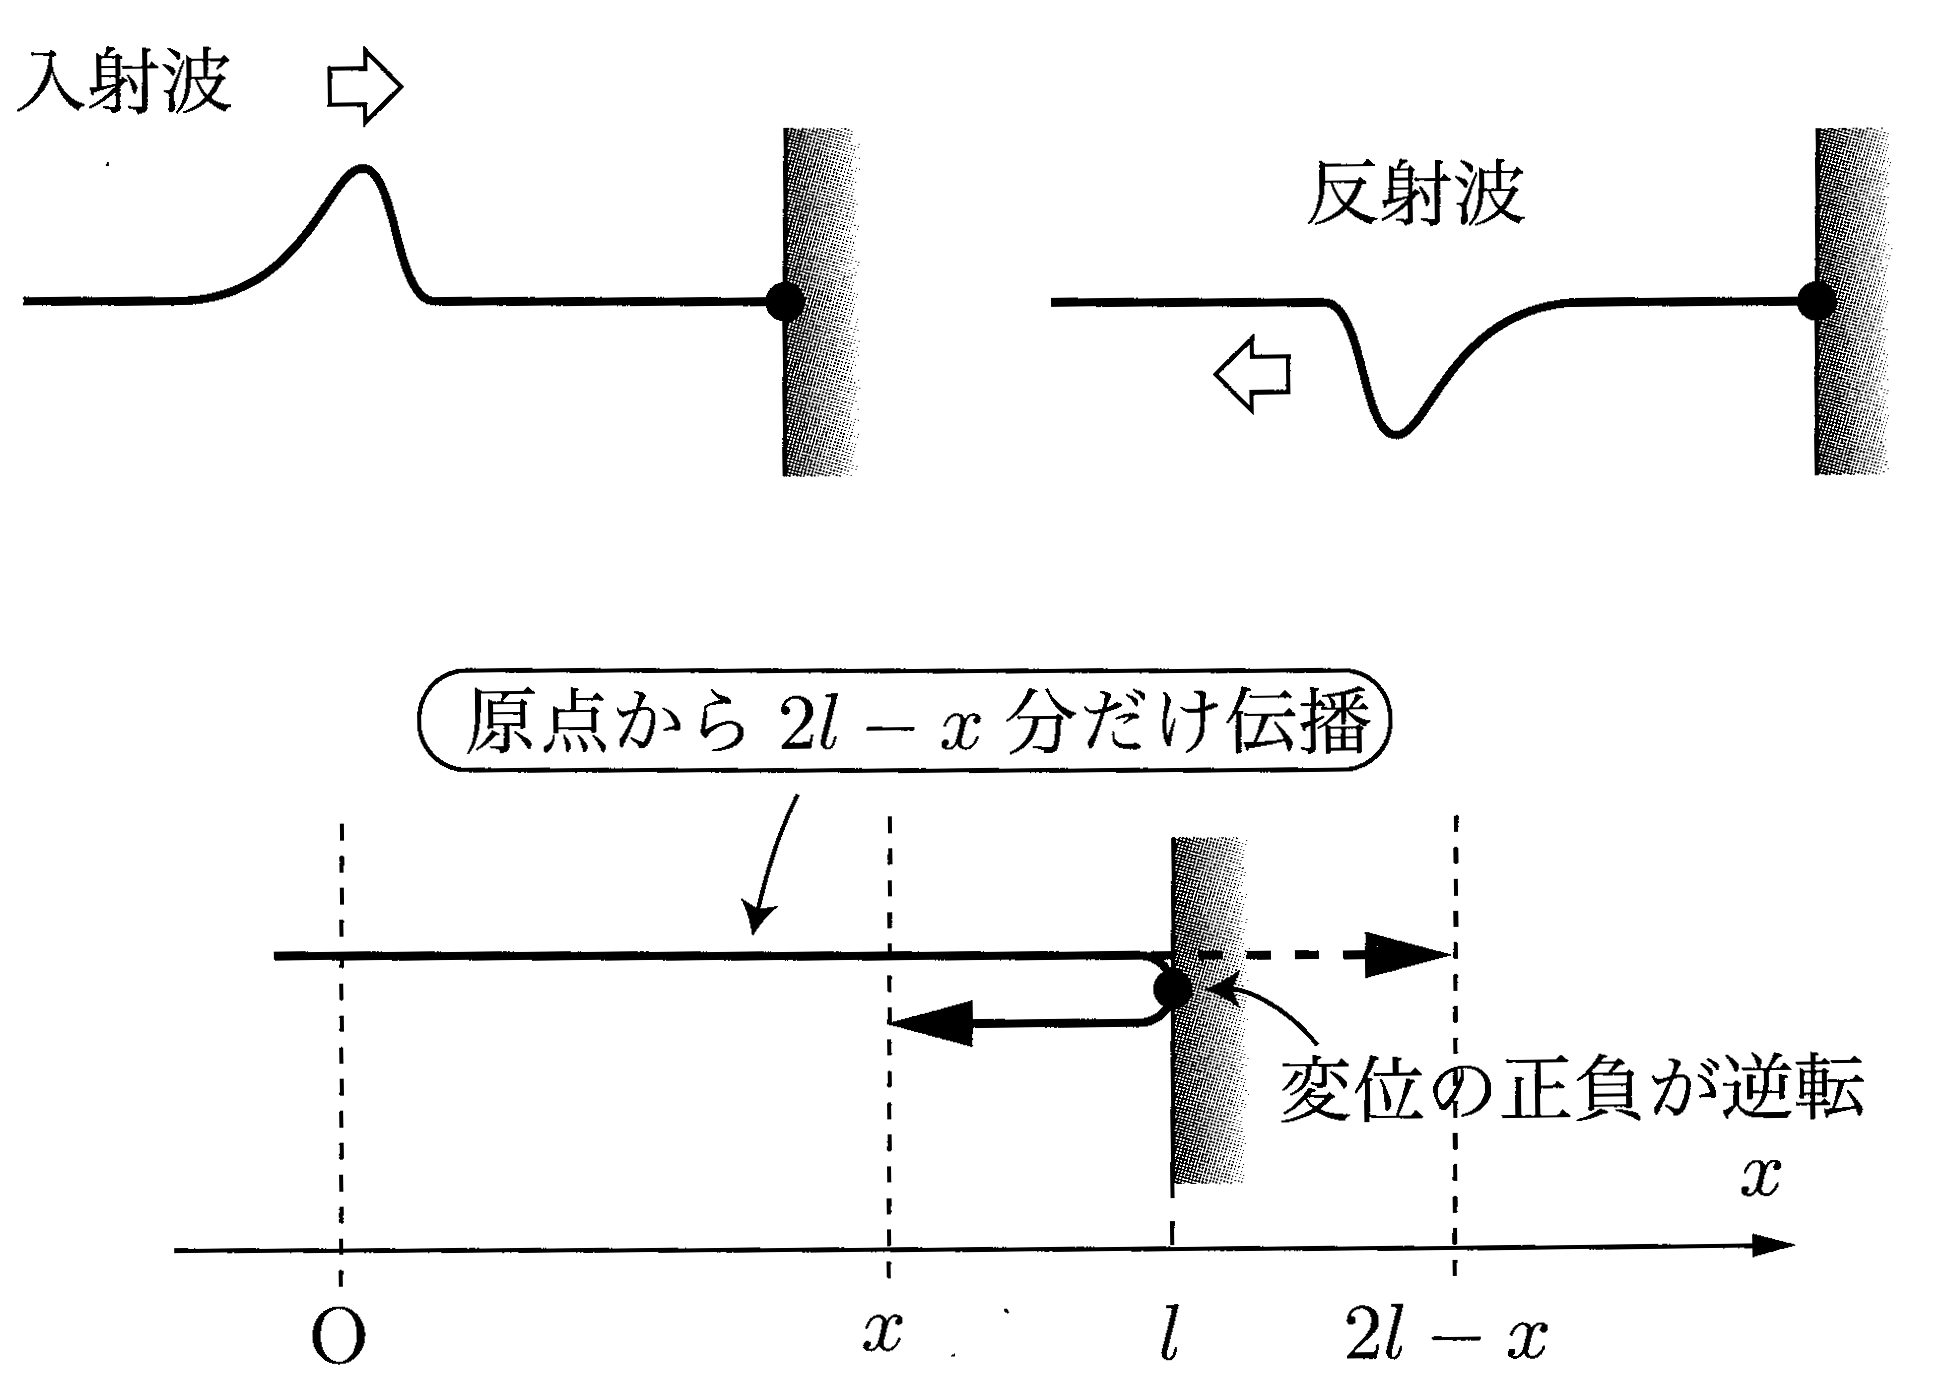
\includegraphics[keepaspectratio,width=80mm]
  {text_p97_fig2.png}
\end{wrapfigure}

\mbox{\boldmath  $反射点にある媒質が固定されている場合，固定端反射となる．$}
反射点が固定されているため，{\bf 入射波と反射波の合成波の変位は0[m]でなければならない．}
そのため，反射点における反射波の変位は，入射波と変位が同じ大きさで逆向きとなり，{\bf 反射波の波形は入射波を反射点で折り返した波形をさらに正負を逆にした波形となる．}

自由端反射の場合と同様に固定端反射された反射波の変位$y'(x,t)$[m]を考えてみよう．
位置$x$[m]における反射波は原点から$2l-x$[m]だけ伝播してきたことは同じであるが，反射点において正負を逆にされているので，
\[y'(x,t)=-y\left( 0,t-\dfrac{2l-x}{v} \right) =-y(2l-x,t)\]
とマイナスをつけることで変位の一般式を求めることができる．
{\bf 反射波の波形は入射波がそのまま直進した場合の波形を反射壁で折り返し，さらに正負を逆にした波形と同じになる．}\\

いずれの反射波の場合でも，反射波は透過波を用いて議論するとよい．

\begin{matome}{反射波の方程式の考え方}
 \hspace{3mm} $\MARU{1}$\hspace{2mm} 反射壁を突き抜ける透過波を考える．\\
 \hspace{3mm} $\MARU{2}$\hspace{2mm} 時刻$t$[s]，位置$x$[m]にいる反射波は，壁面を透過していたらその時刻にどこにいるかを考える．\\
 \hspace{3mm} $\MARU{3}$\hspace{2mm} 反射壁で反射される際に，そのまま反射されるのか，上下反転されるのかを把握する．\\
 \hspace{3mm} $\MARU{4}$\hspace{2mm} 方程式を立てる．
 \end{matome}

\subsection{入射波と反射波によって作られる定常波}
一直線上を進む正弦波が反射壁によって完全に反射する（＝減衰せずに反射する）場合，入射波と反射波は同一振幅・波長・振動数で互いに逆向きに進むから，この2つが重なってできる合成波は定常波となる．
定常波は，腹・腹間隔＝節・節間隔$=\dfrac{\lambda}{2}$，腹・節間隔$=\dfrac{\lambda}{4}$なる間隔で，節と腹とが交互に並ぶものであるが，
\begin{description}
\item[・] {\bf 自由端反射の反射点}\\
{\bf 入射波がそのまま反射}\hspace{2mm}$\Leftrightarrow$\hspace{2mm}{\bf 合成波の変位は常に入射波の変位の2倍}\hspace{2mm}$\Leftrightarrow$\hspace{2mm}{\bf 定常波の腹}
\item[・] {\bf 固定端反射の反射点}\\
{\bf 媒質は動けない}\hspace{2mm}$\Leftrightarrow$\hspace{2mm}{\bf 合成波の変位は常に0}\hspace{2mm}$\Leftrightarrow$\hspace{2mm}{\bf 定常波の節}
\end{description}
となっている．
そのため，自由端反射，固定端反射によってできる定常波の波形は次の図のようになる．
 \begin{figure}[h]
\begin{center}
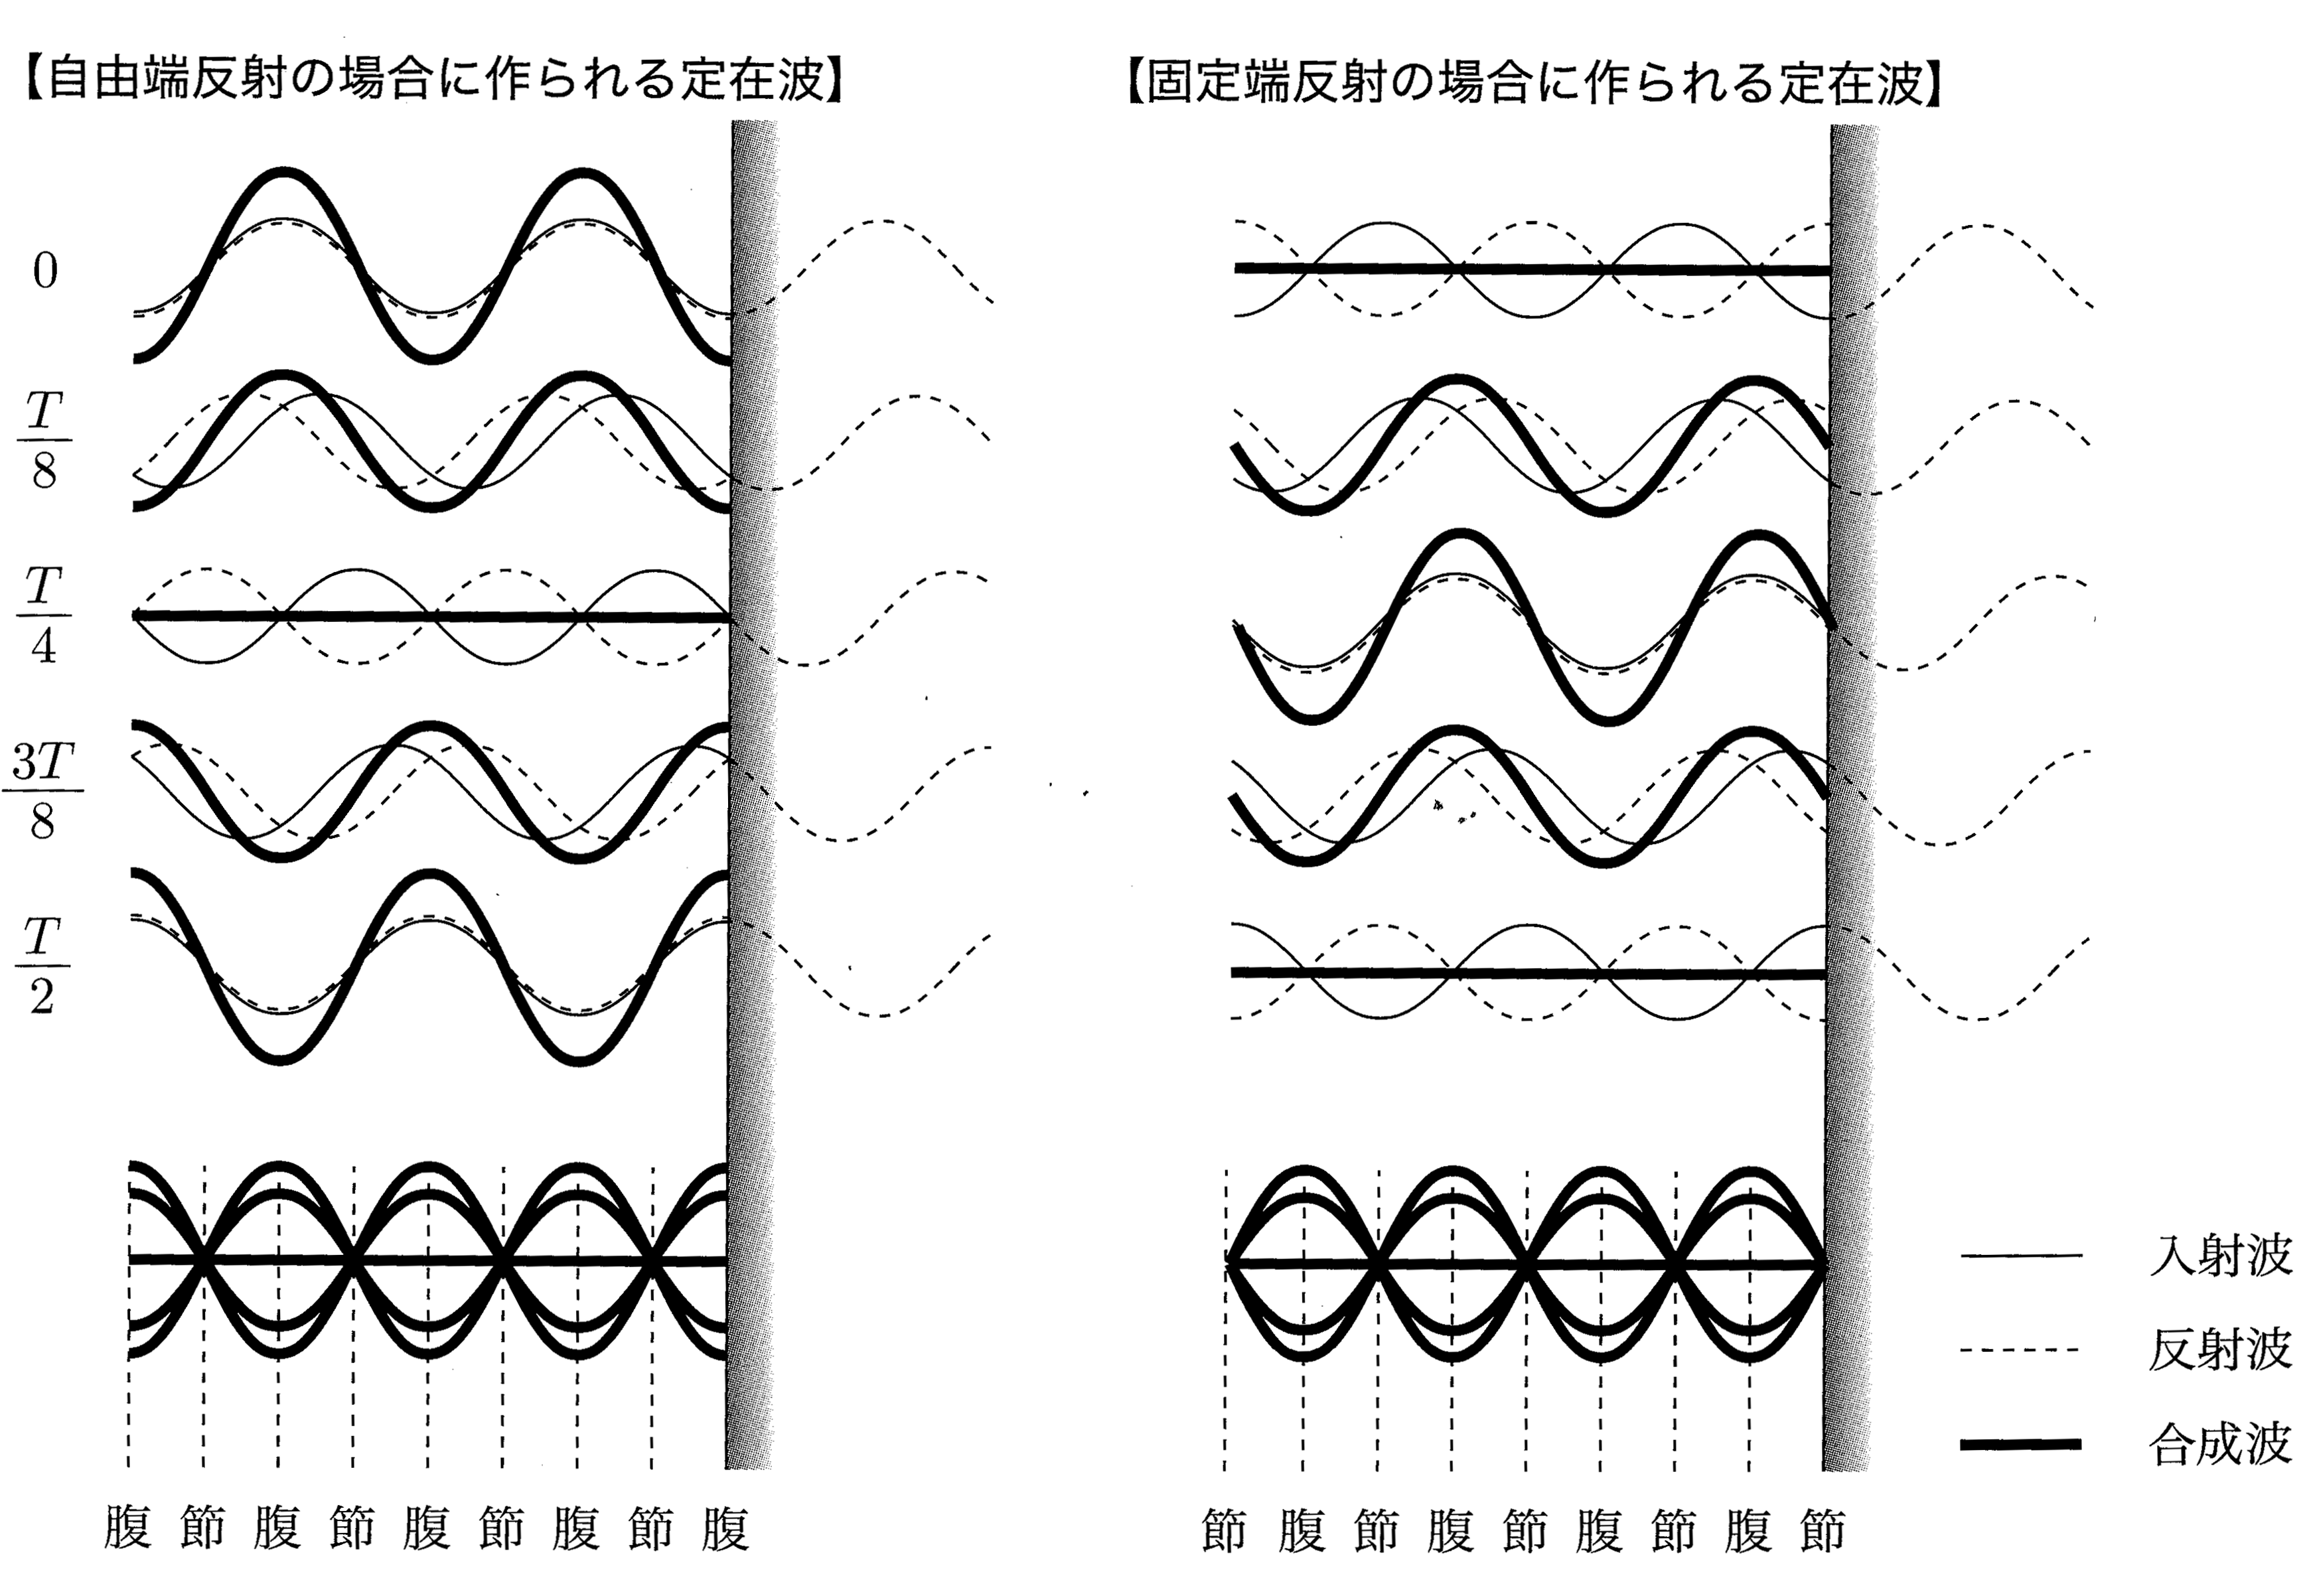
\includegraphics[width=140mm]{text_p99_fig1.png}
\end{center}
\end{figure}

\subsection{定常波の表式}
互いに逆向きに進む振幅$A$[m]，波長$\lambda$[m]，周期$T$[s]の正弦波が重なって作られる定常波は，
\[y(x,t)=2A\sin\left( 2\pi \dfrac{x}{\lambda} +\varphi_1 \right) \sin \left( 2\pi\dfrac{t}{T} +\varphi_2 \right) \]
の形に表すことができる．（ただし$\varphi_1,\varphi_2$は条件を満たすようにとる定数）

この式の第2項の$\sin$部分である$\sin \left( 2\pi\dfrac{t}{T} +\varphi_2 \right)$は時刻$t$[s]の進行につれて$-1〜+1$の範囲で振動する．
よって，位置$x$[m]におけるこの定常波の振幅$A(x)$[m]は
\[A(x)=2A\left| \sin\left( 2\pi \dfrac{x}{\lambda} +\varphi_1 \right)\right|\]
で与えられ，この位置では定常波は$-A(x)〜+A(x)$の範囲を振動する．
また，時間変動をもたらす第2項の$ \sin \left( 2\pi\dfrac{t}{T} +\varphi_2 \right)$はすべての$x$に対して同等にかかるから，定常波は各点が同じ位相で上下に振動することになることもこの式から理解することができる．
\begin{matome}{定常波の表式}
 \hspace{3mm} 互いに逆向きに進む振幅$A$[m]，波長$\lambda$[m]，周期$T$[s]の正弦波が重なって作られる定常波は，
 \[y(x,t)=2A\sin\left( 2\pi \dfrac{x}{\lambda} +\varphi_1 \right) \sin \left( 2\pi\dfrac{t}{T} +\varphi_2 \right) \]
 の形に必ず表せ，位置による振幅を表す部分と時間変動して$-1〜+1$の範囲で振動する部分とに分けることができる．
\end{matome}

\newpage

\begin{figure}[h]
\begin{center}
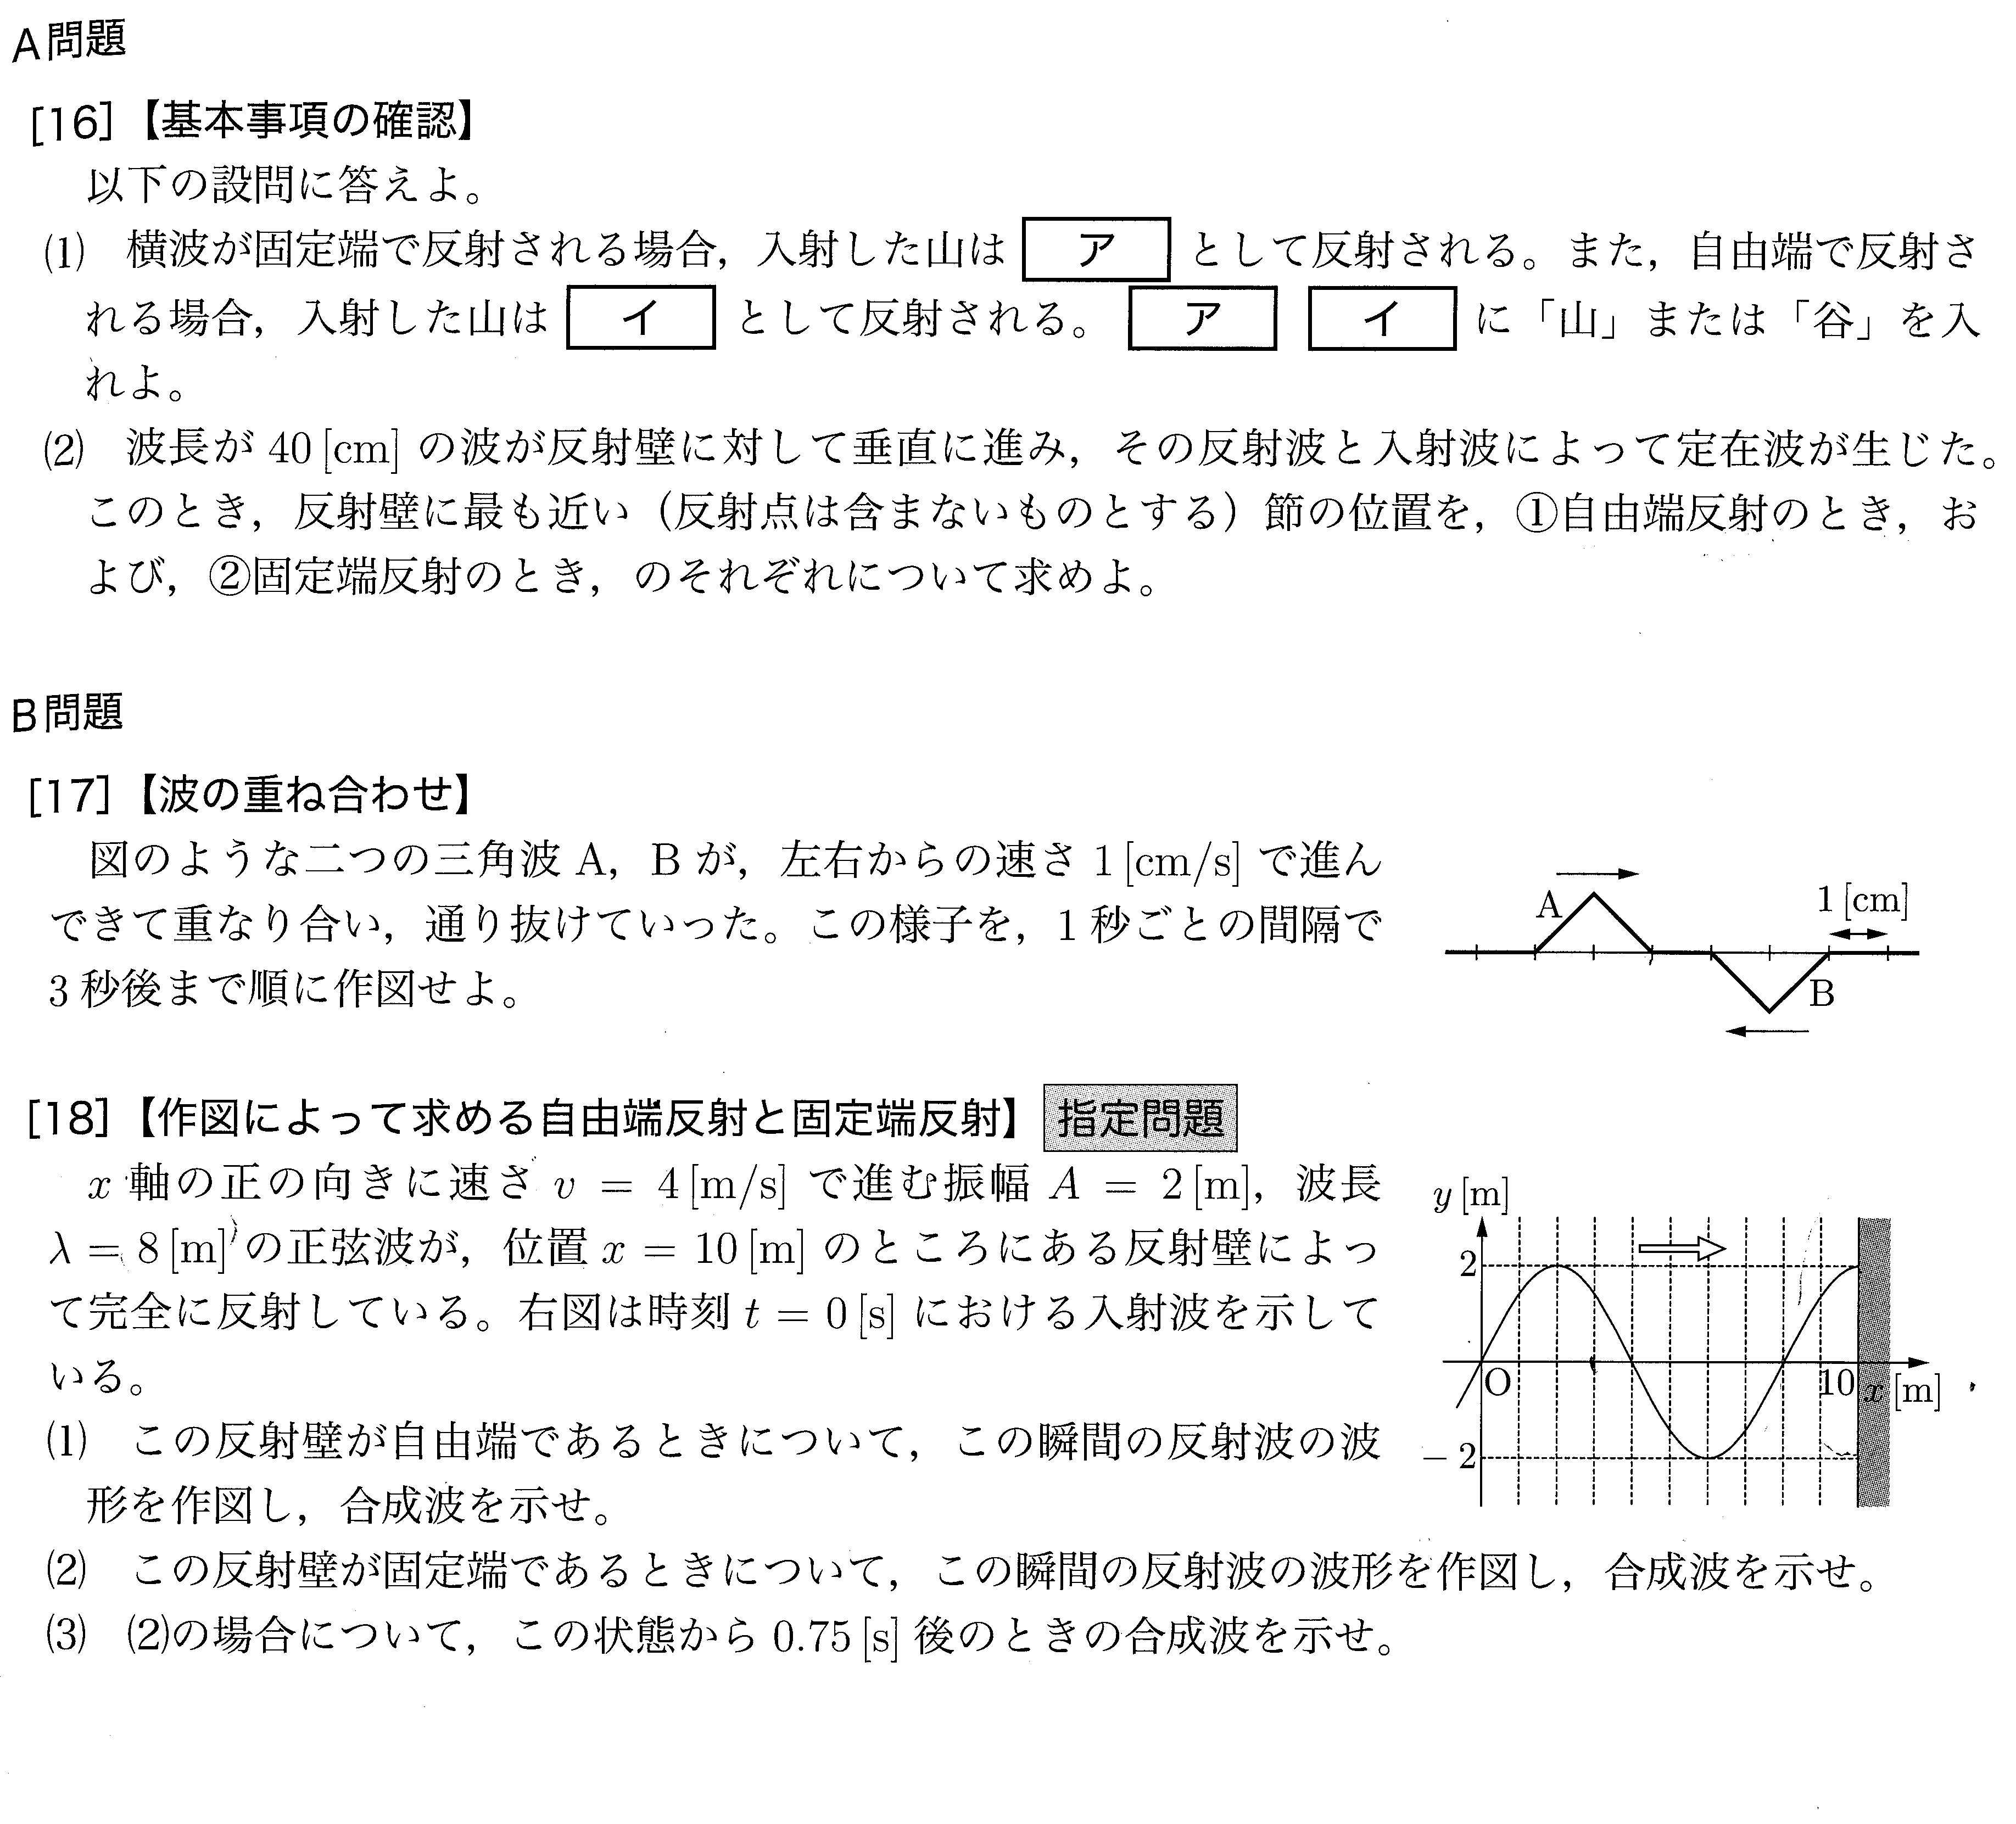
\includegraphics[width=170mm]{prob_p53.png}
\vspace{150mm}
\end{center}
\end{figure}

\newpage

\begin{figure}[h]
\begin{center}
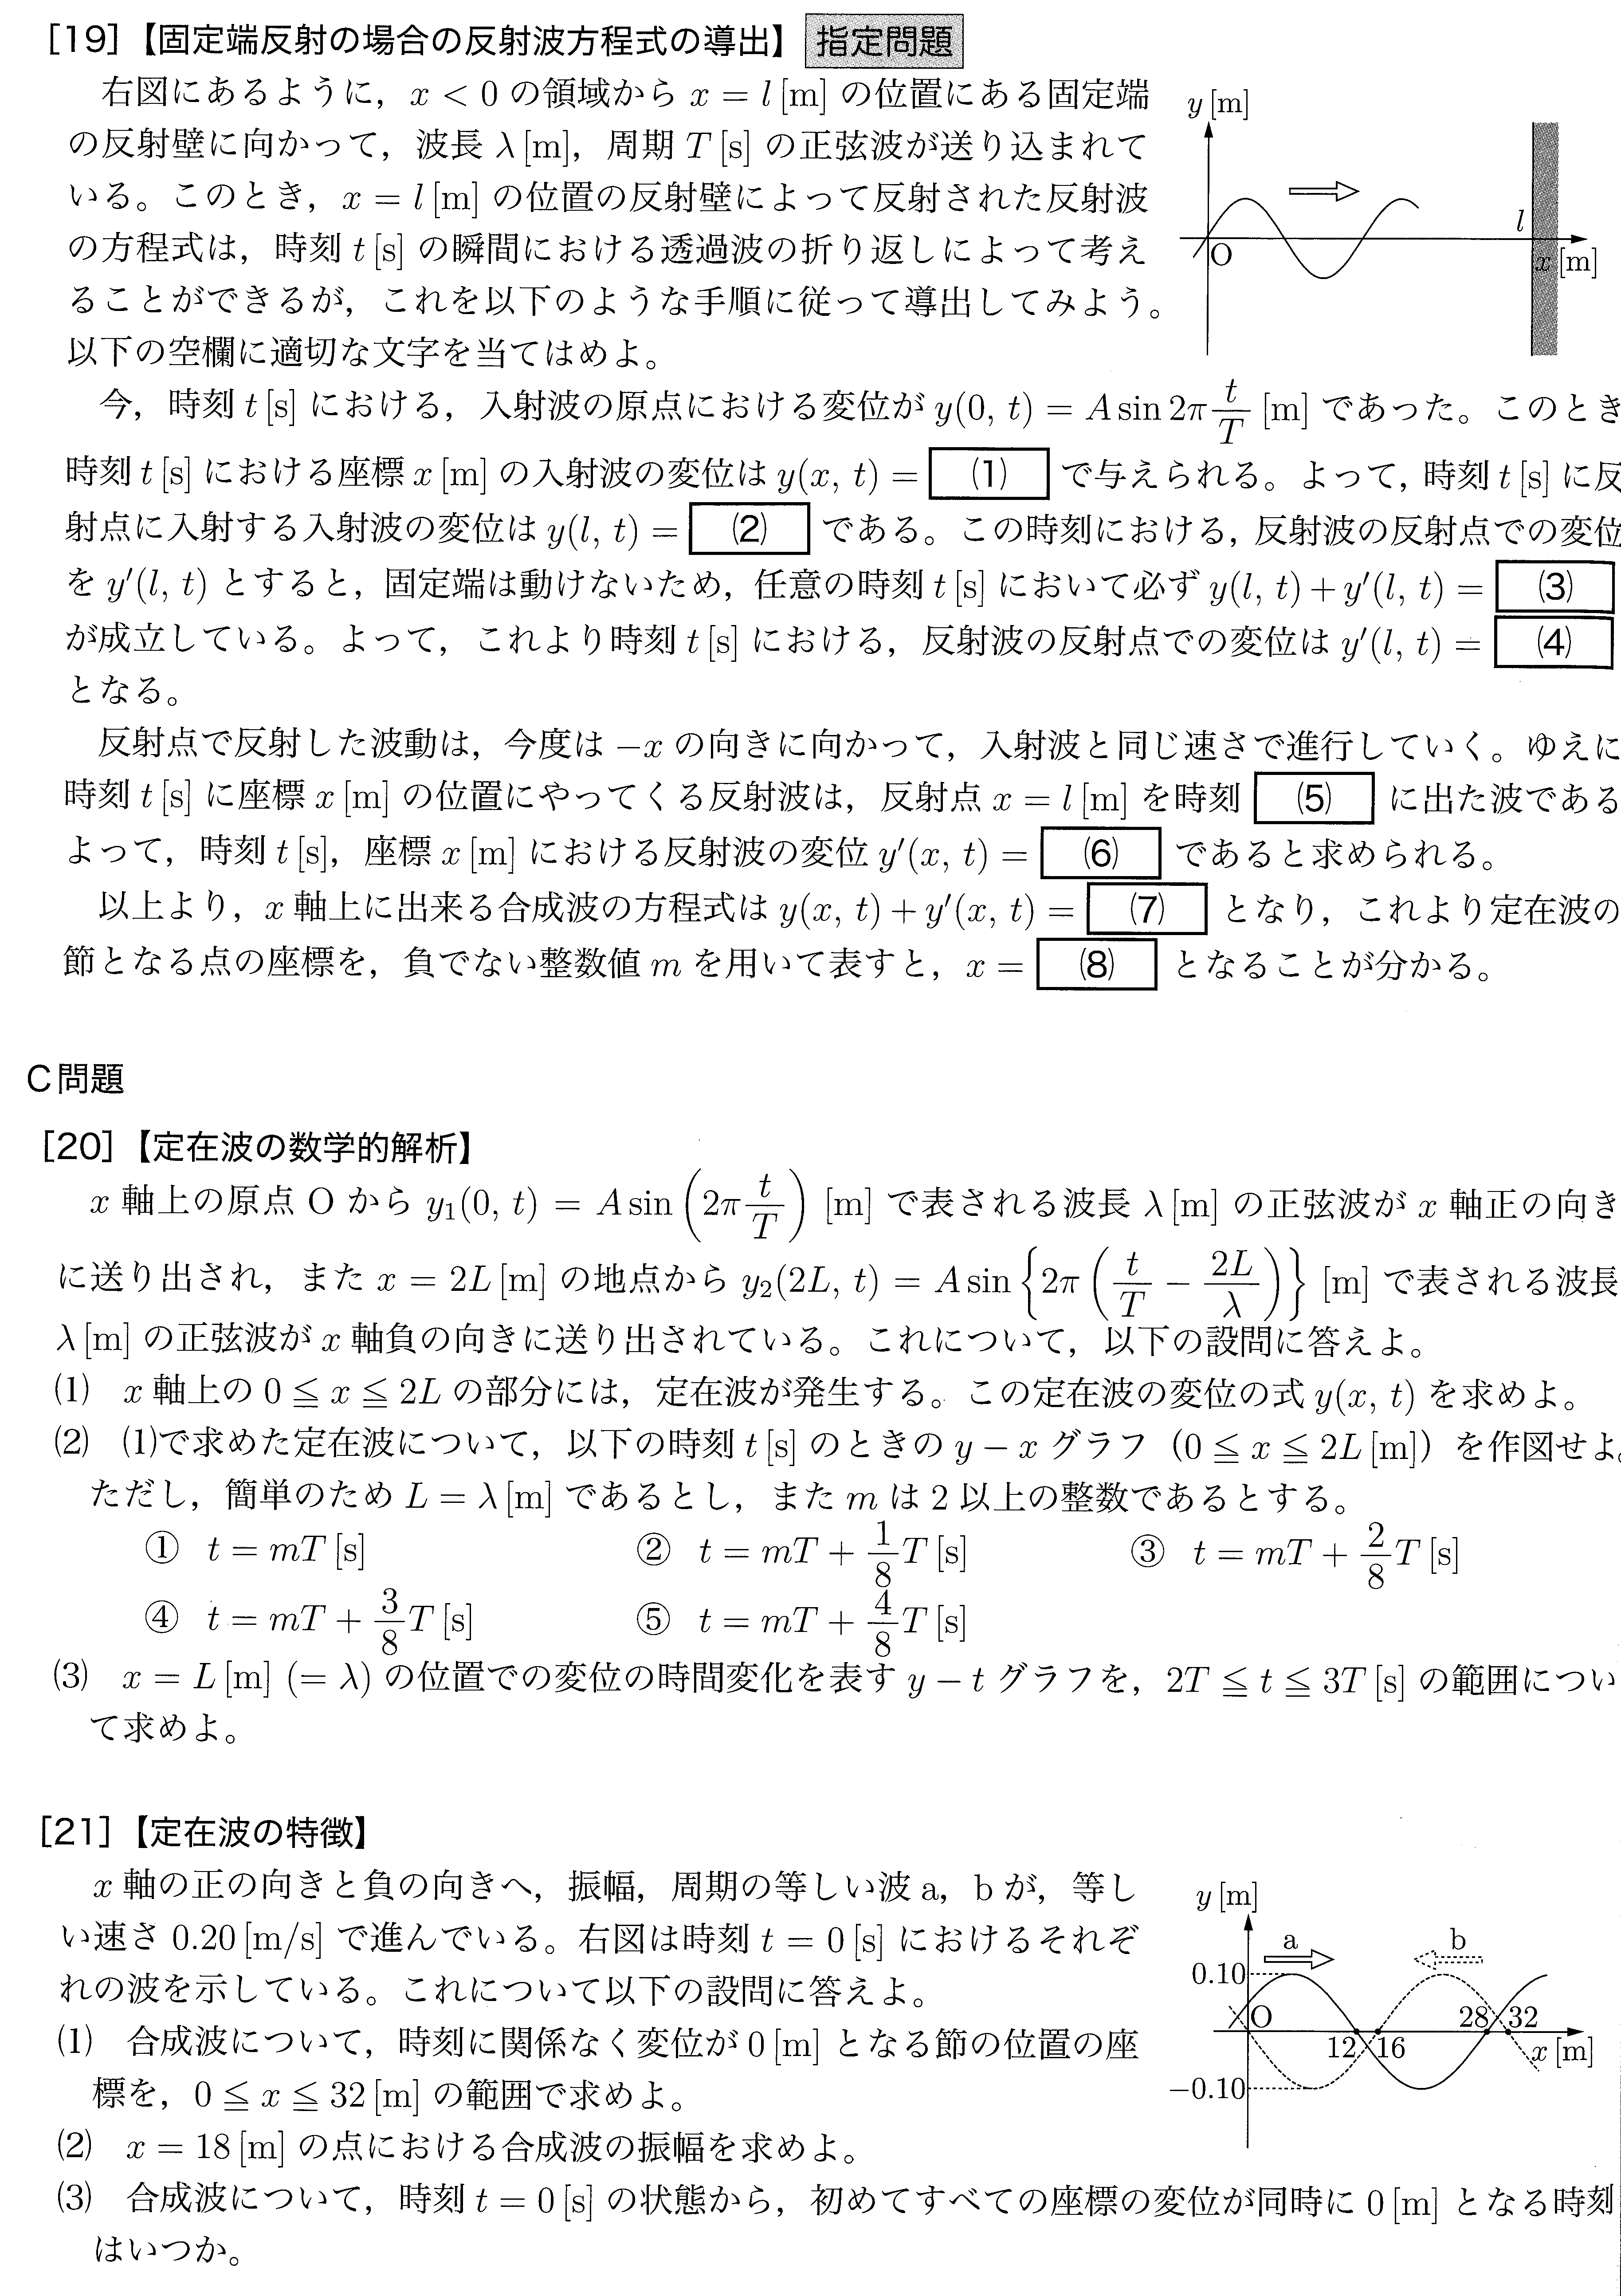
\includegraphics[width=170mm]{prob_p54.png}
\vspace{150mm}
\end{center}
\end{figure}

\newpage

\begin{figure}[h]
\begin{center}
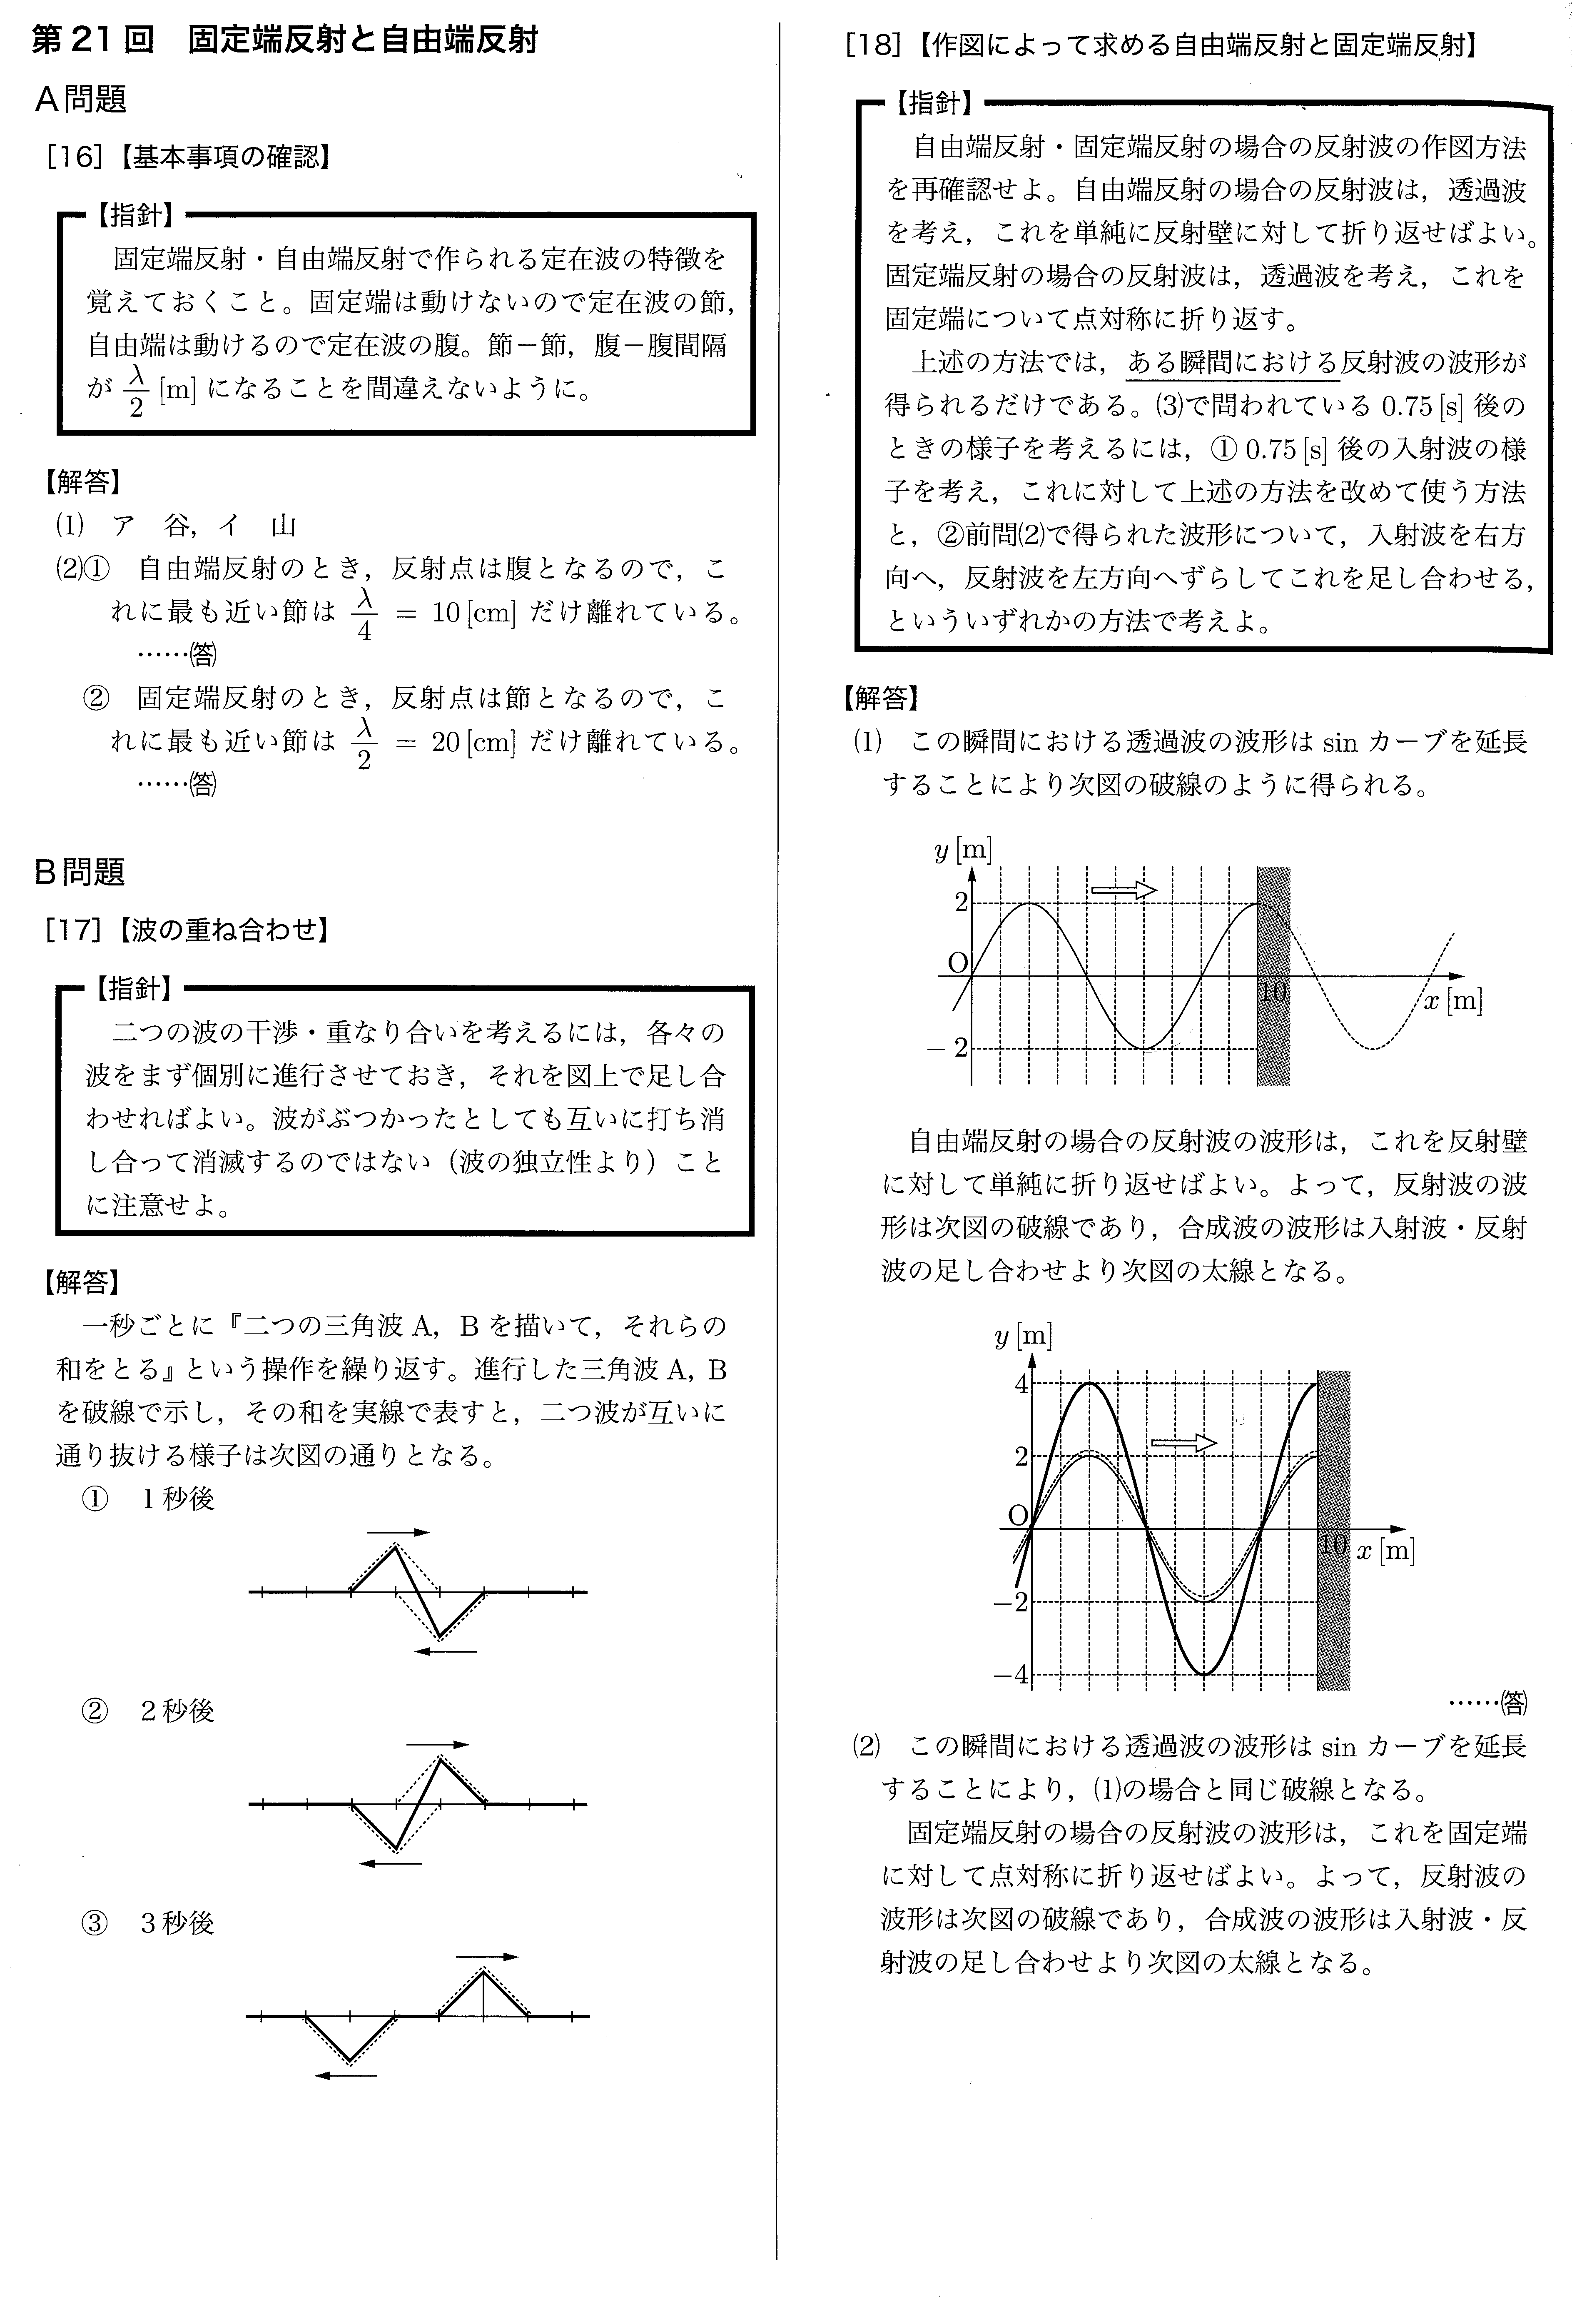
\includegraphics[width=170mm]{prob_p154.png}
\vspace{150mm}
\end{center}
\end{figure}

\newpage

\begin{figure}[h]
\begin{center}
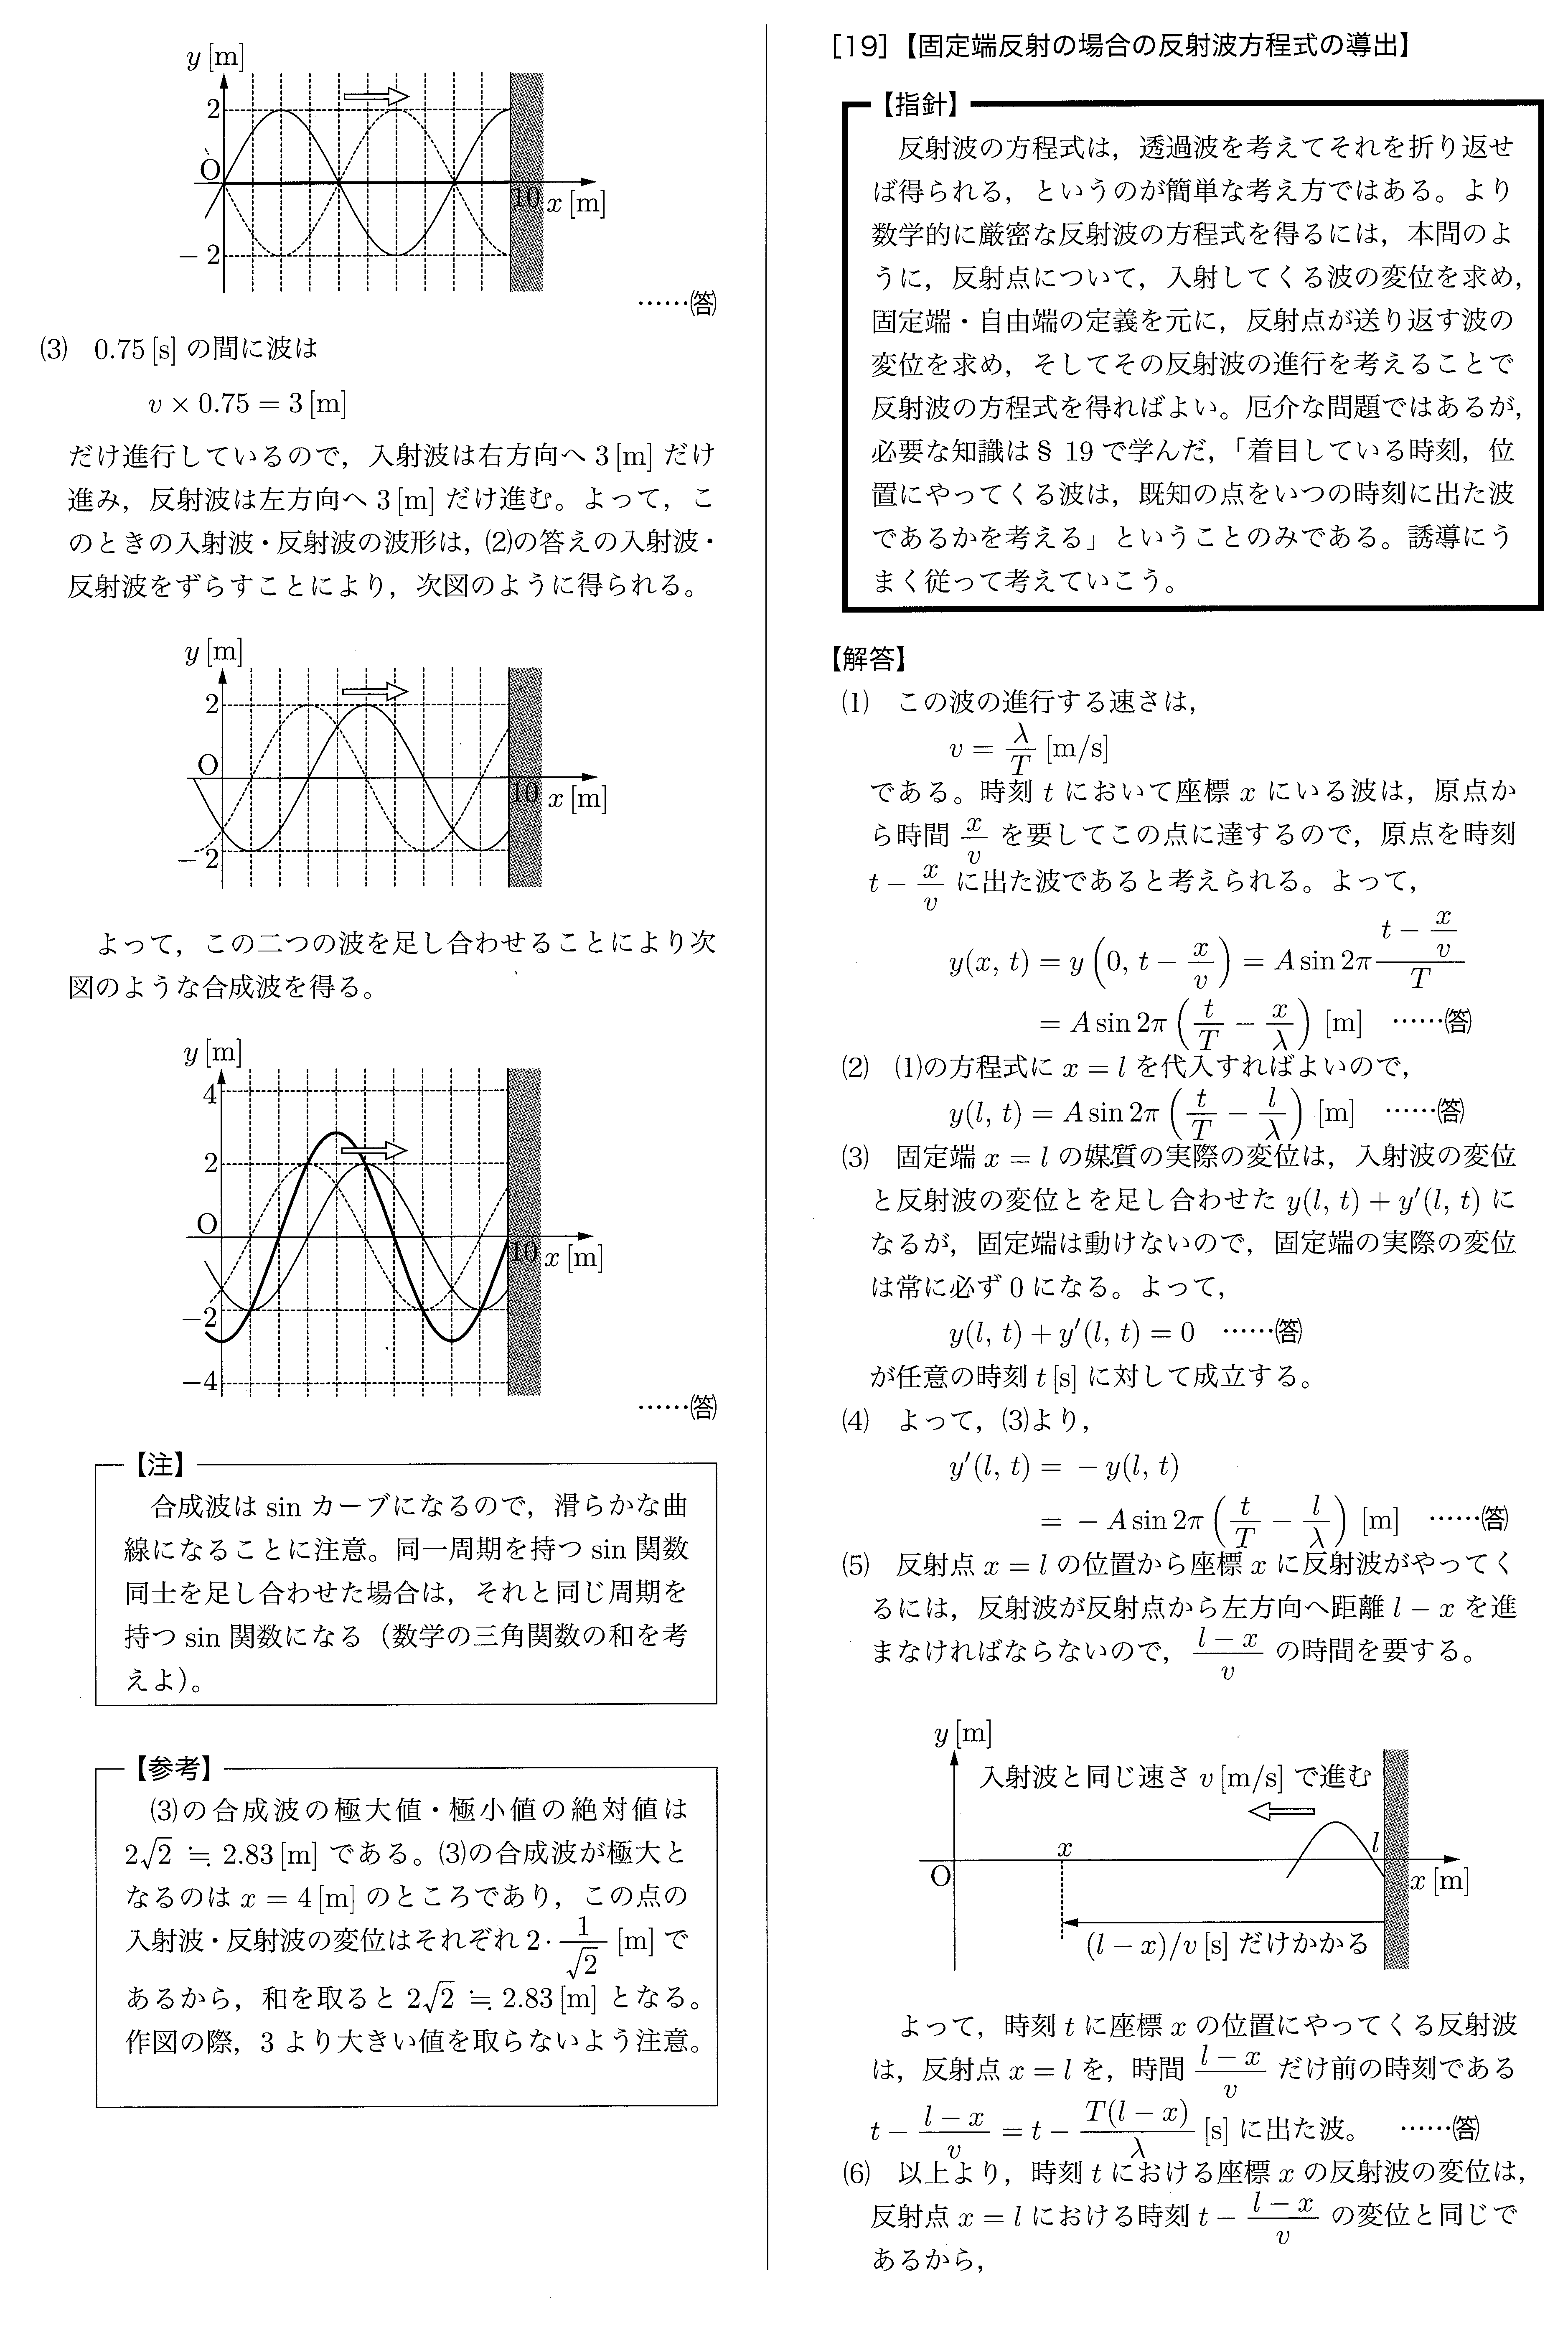
\includegraphics[width=170mm]{prob_p155.png}
\vspace{150mm}
\end{center}
\end{figure}

\newpage

\begin{figure}[h]
\begin{center}
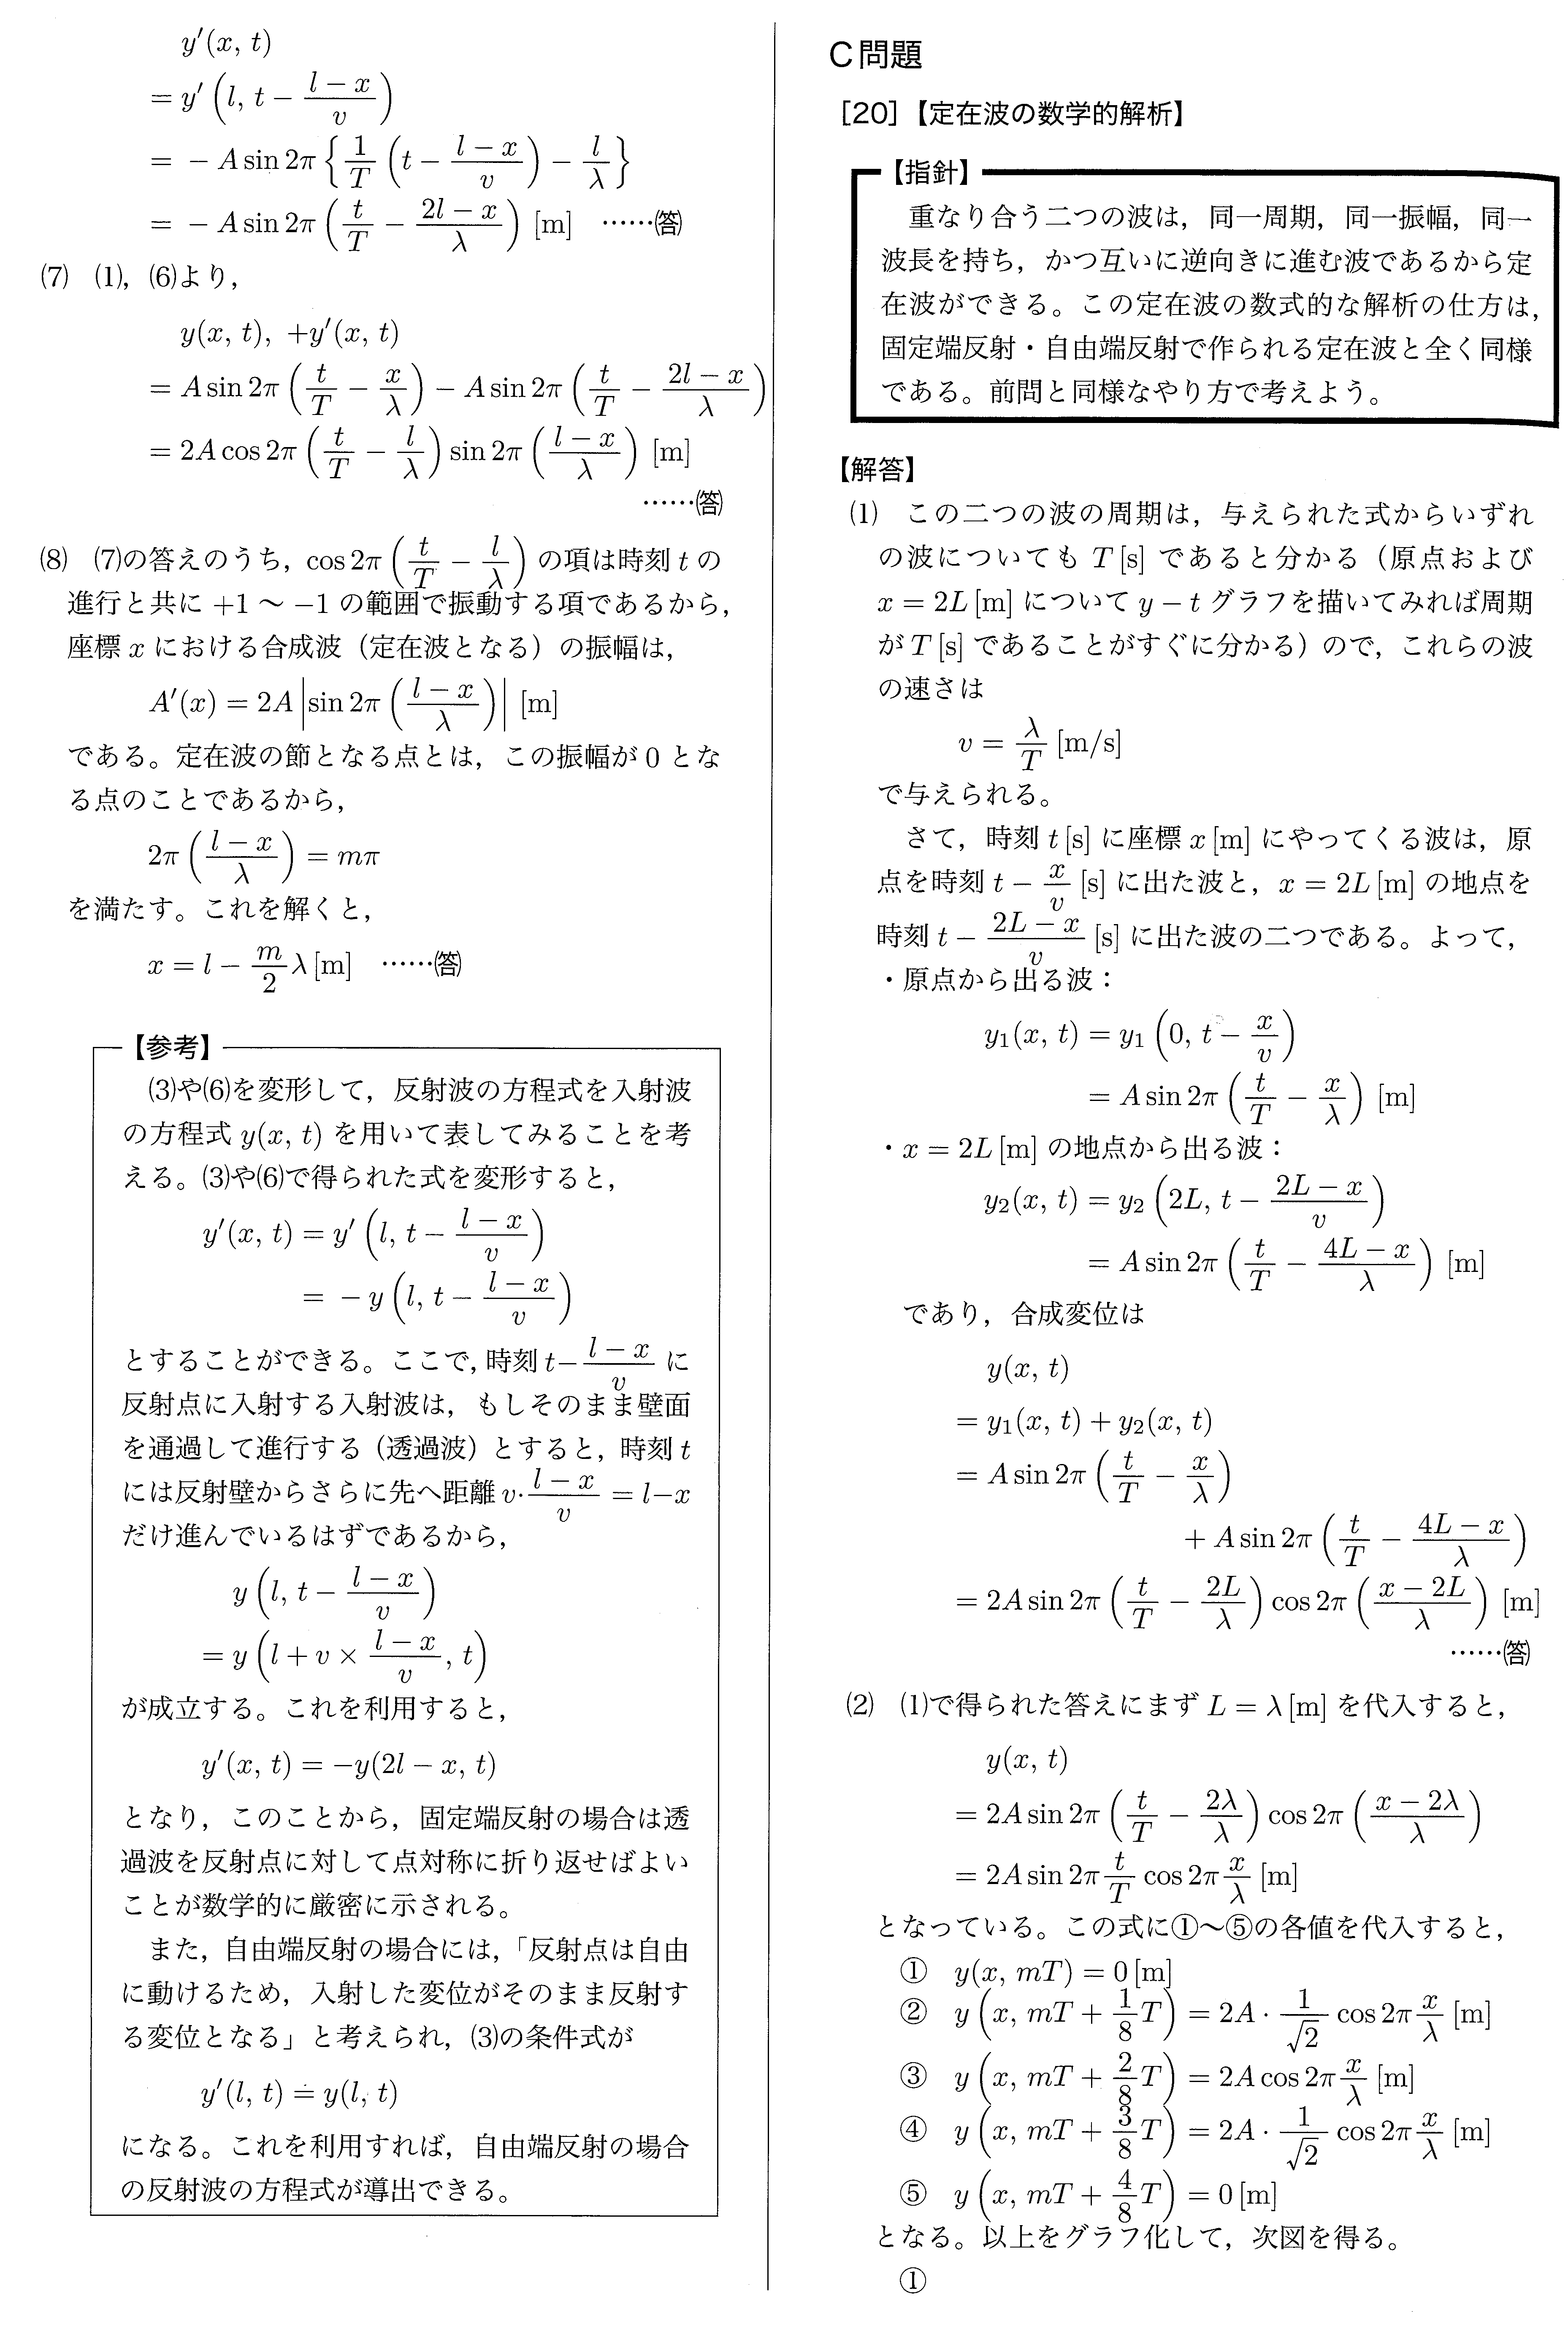
\includegraphics[width=170mm]{prob_p156.png}
\vspace{150mm}
\end{center}
\end{figure}

\newpage

\begin{figure}[h]
\begin{center}
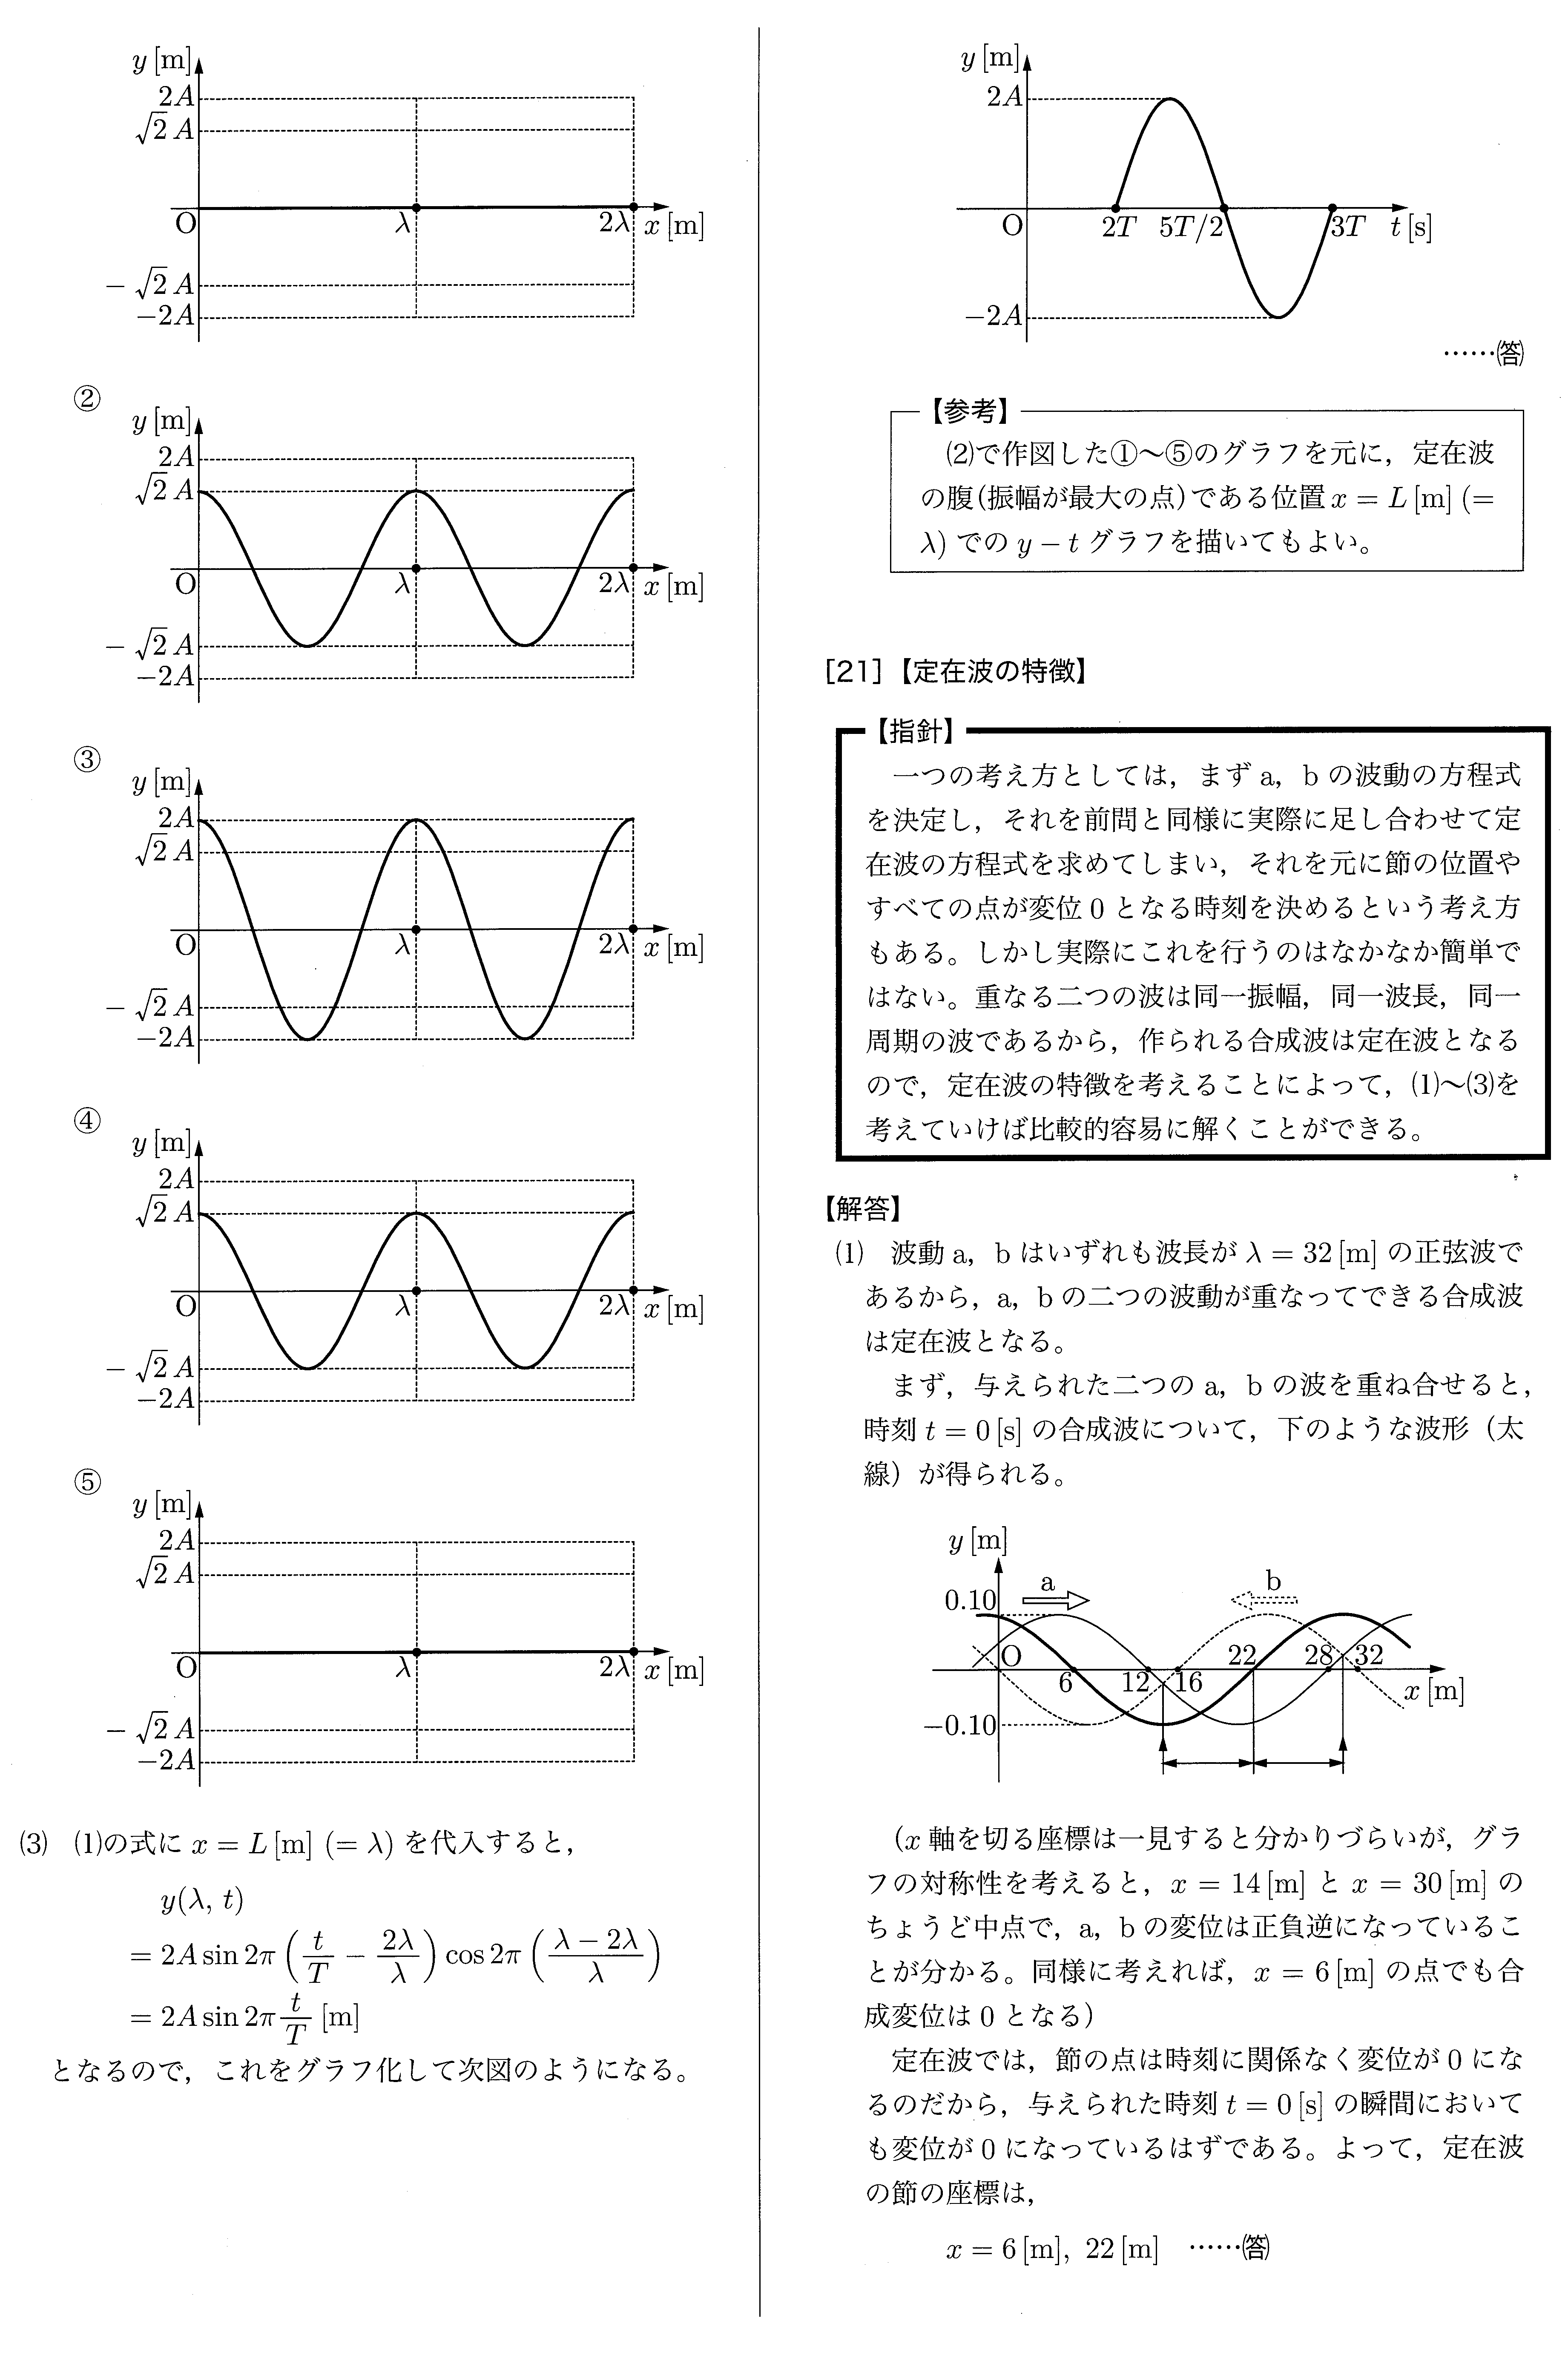
\includegraphics[width=170mm]{prob_p157.png}
\vspace{150mm}
\end{center}
\end{figure}

\newpage

\begin{figure}[h]
\begin{center}
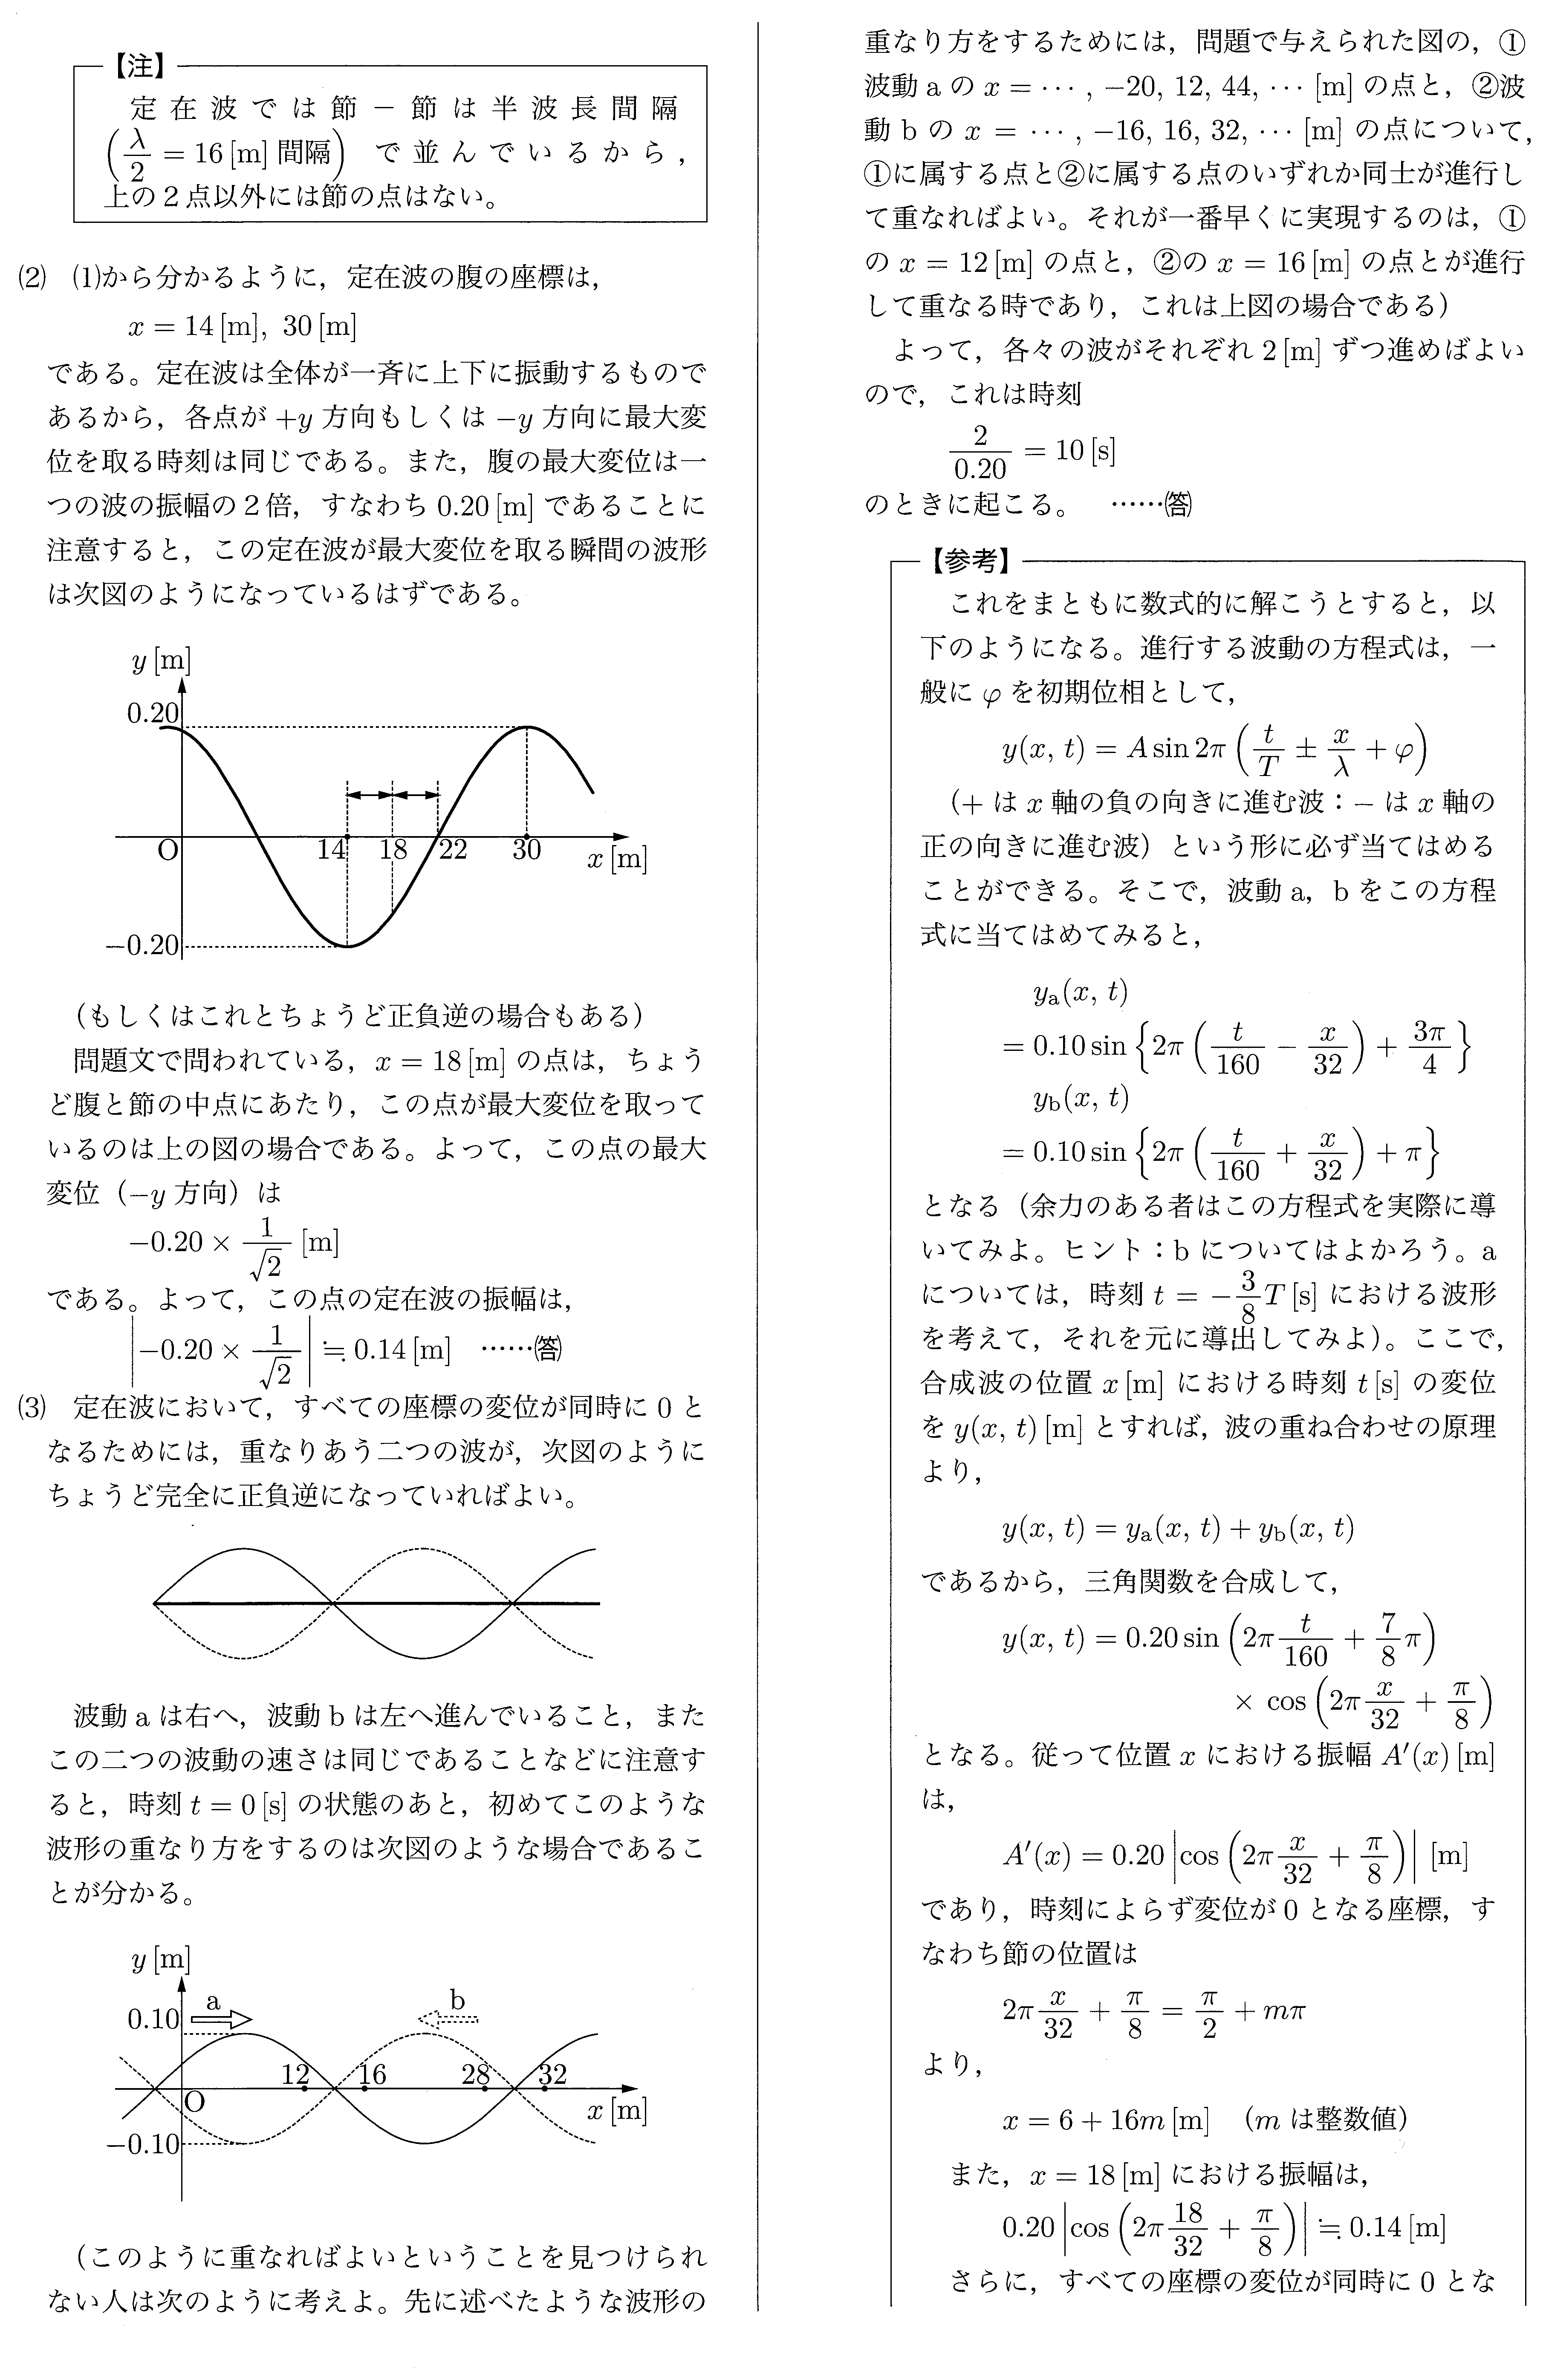
\includegraphics[width=170mm]{prob_p158.png}
\vspace{150mm}
\end{center}
\end{figure}

\newpage

\begin{figure}[h]
\begin{center}
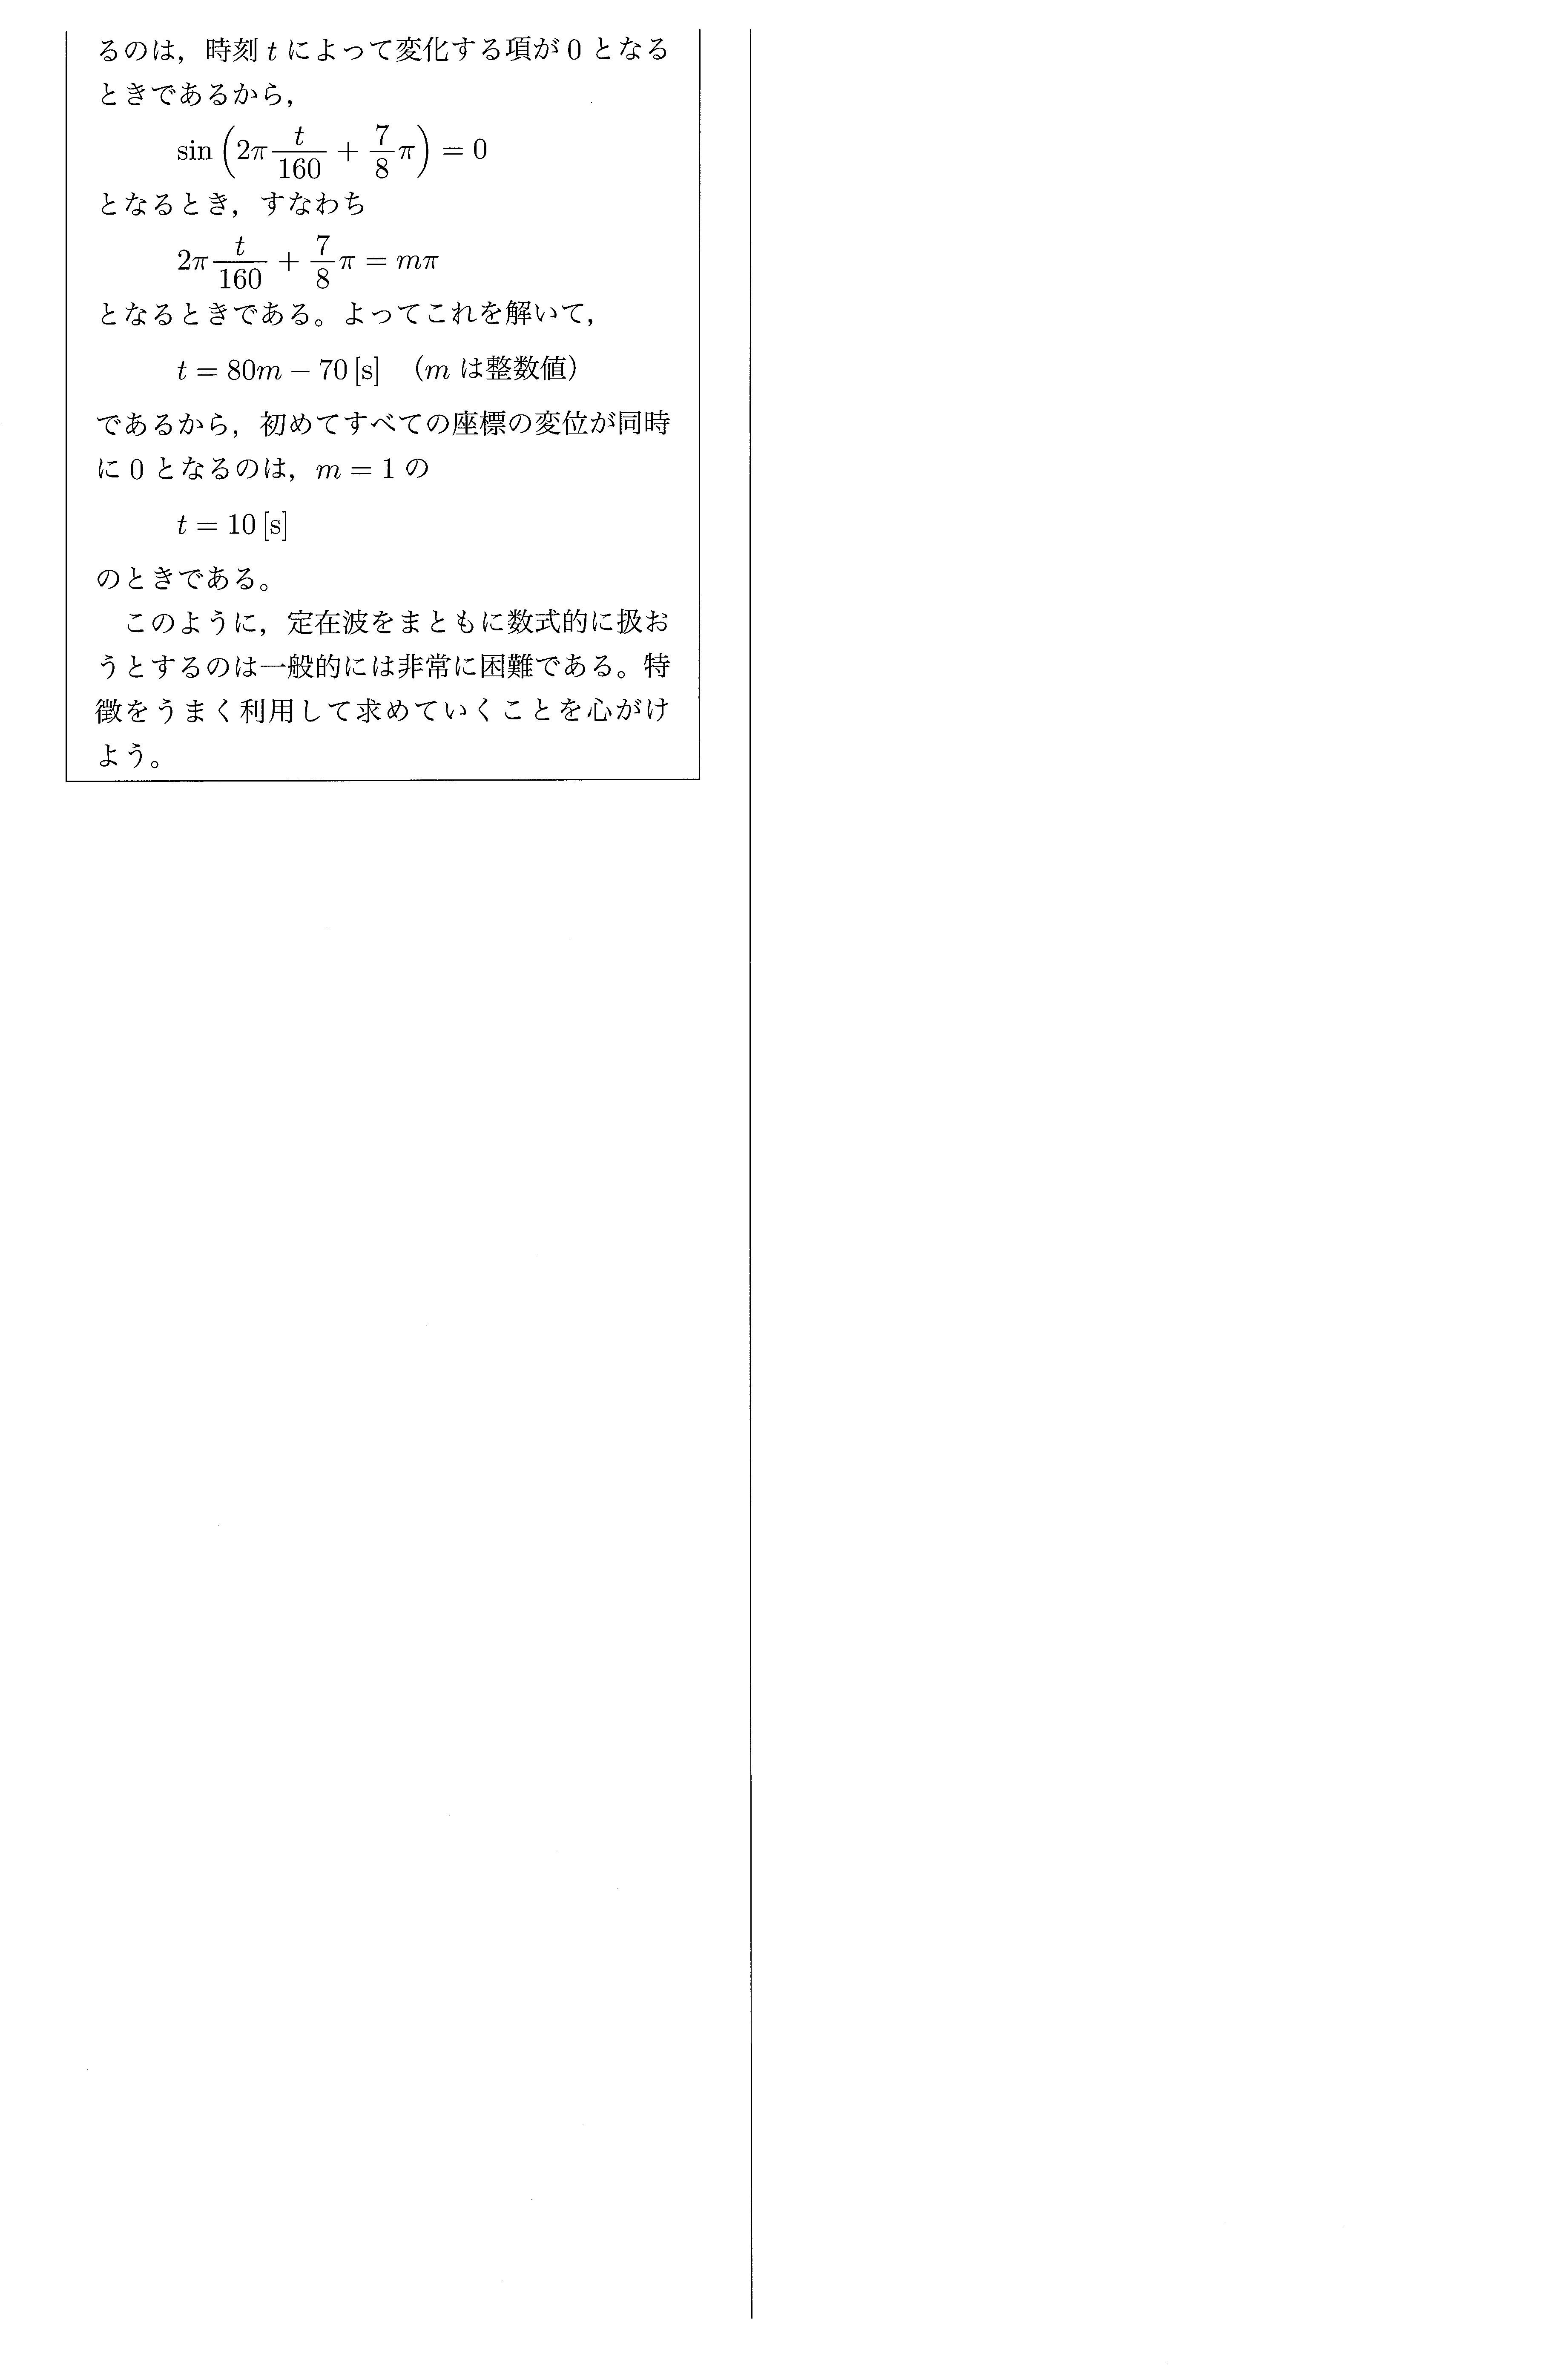
\includegraphics[width=170mm]{prob_p159_1.png}
\vspace{150mm}
\end{center}
\end{figure}
 \ 
 
\newpage
\include{physics_ch22}
\include{physics_ch23}
 \ 
 
\newpage
\section{ドップラー効果(2)・屈折の法則}

\subsection{斜めドップラー効果}
ここまでは波源と観測者が，その2点を結ぶ直線方向のみに運動する場合を考えたが，それ以外の方向に波源・観測者が運動する場合は，波源と観測者の速度のうち，波の伝播方向の速度成分のみがドップラー効果に寄与する．

\begin{wrapfigure}[8]{r}[5mm]{90mm}
  \centering
  \vspace{-5mm}
  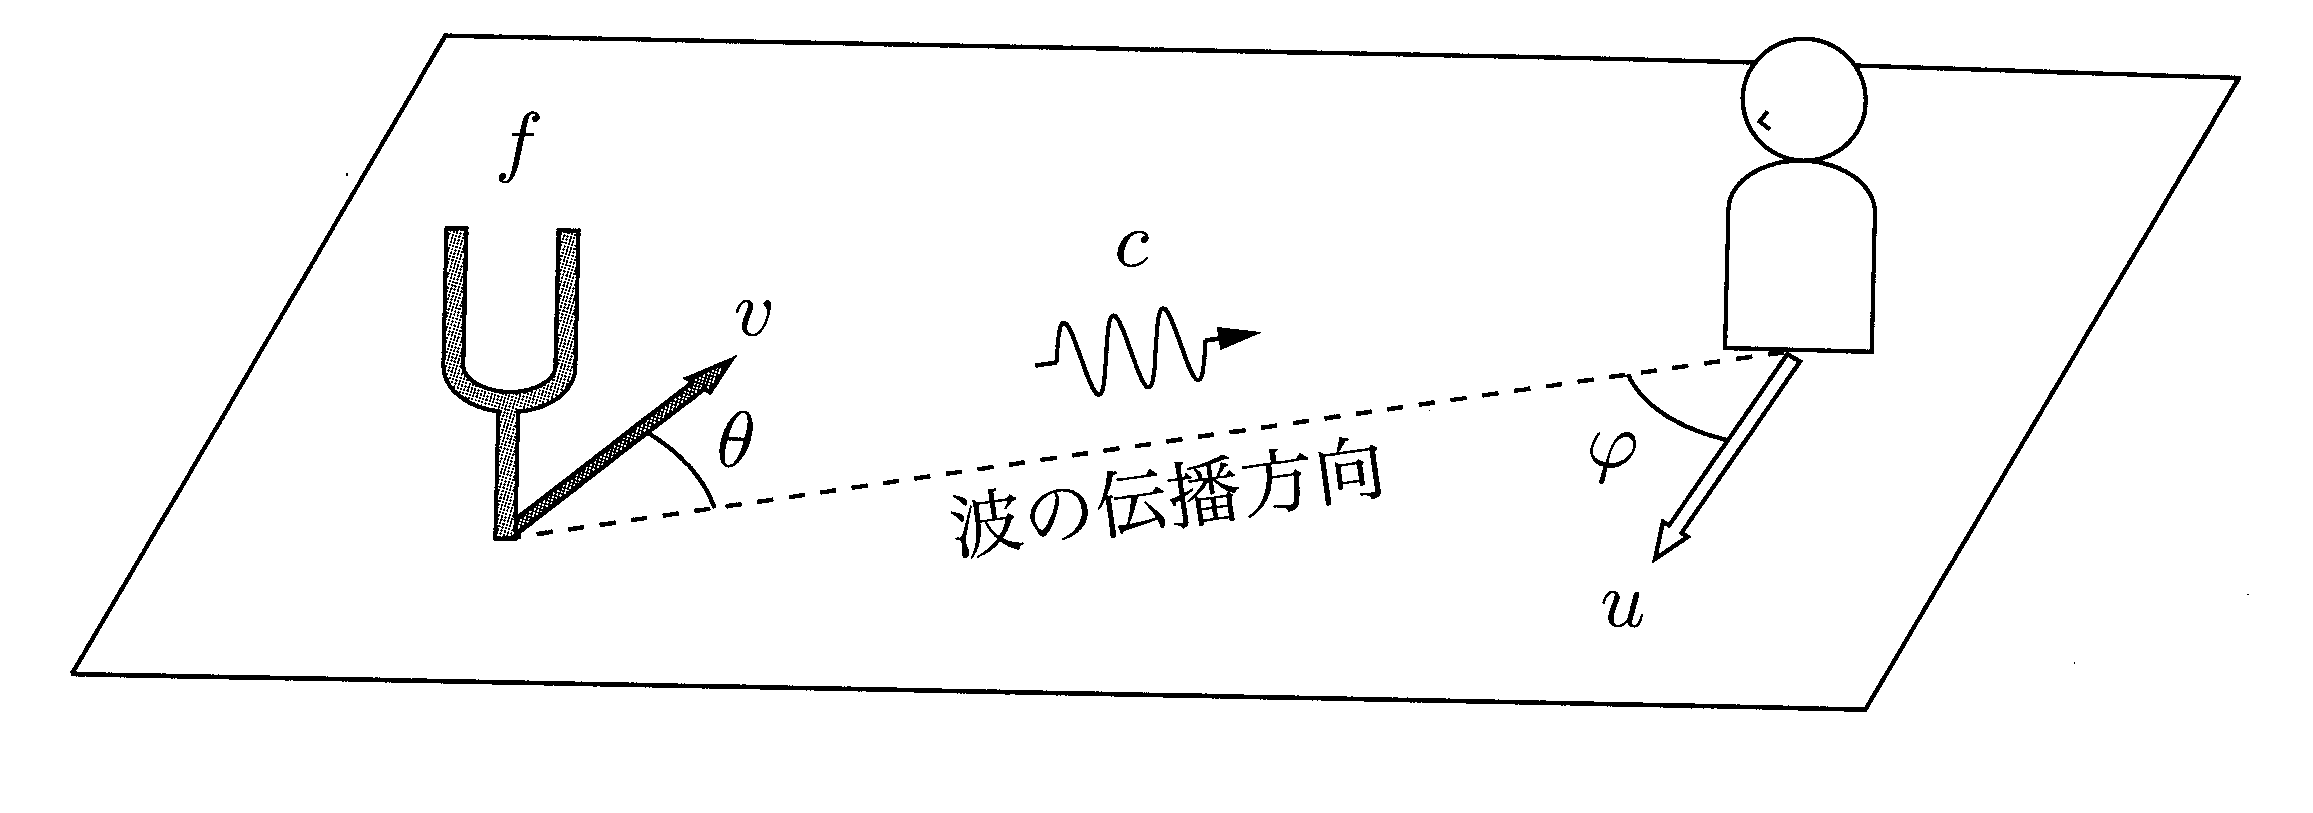
\includegraphics[keepaspectratio,width=90mm]
  {text_p113_fig1.png}
\end{wrapfigure}
例えば，右図のように波源と観測者が運動する場合は，波の伝播方向の速度成分である$v\cos \theta$[m/s]および$u\cos \varphi$[m/s]がドップラー効果に有効な速度成分であるから，
\[f'=\dfrac{c+u\cos\varphi}{c-v\cos \theta} f \hspace{2mm}[{\rm Hz}]\]
となる振動数の音が観測される．

\subsection{衝撃波}
今まで考えてきたドップラー効果はいずれも波源の速さが波の速さを超えない場合であった．
もし波源の速さが波の速さを超えるようになると，波源の前方へ進む波の波長はドップラー効果の式から計算すると負になってしまう．
すなわち，{\bf 波源の速さが波の速さを超えると波源の前方ではドップラー効果は起こらない．}

\begin{wrapfigure}[18]{r}[5mm]{65mm}
  \centering
  \vspace{-5mm}
  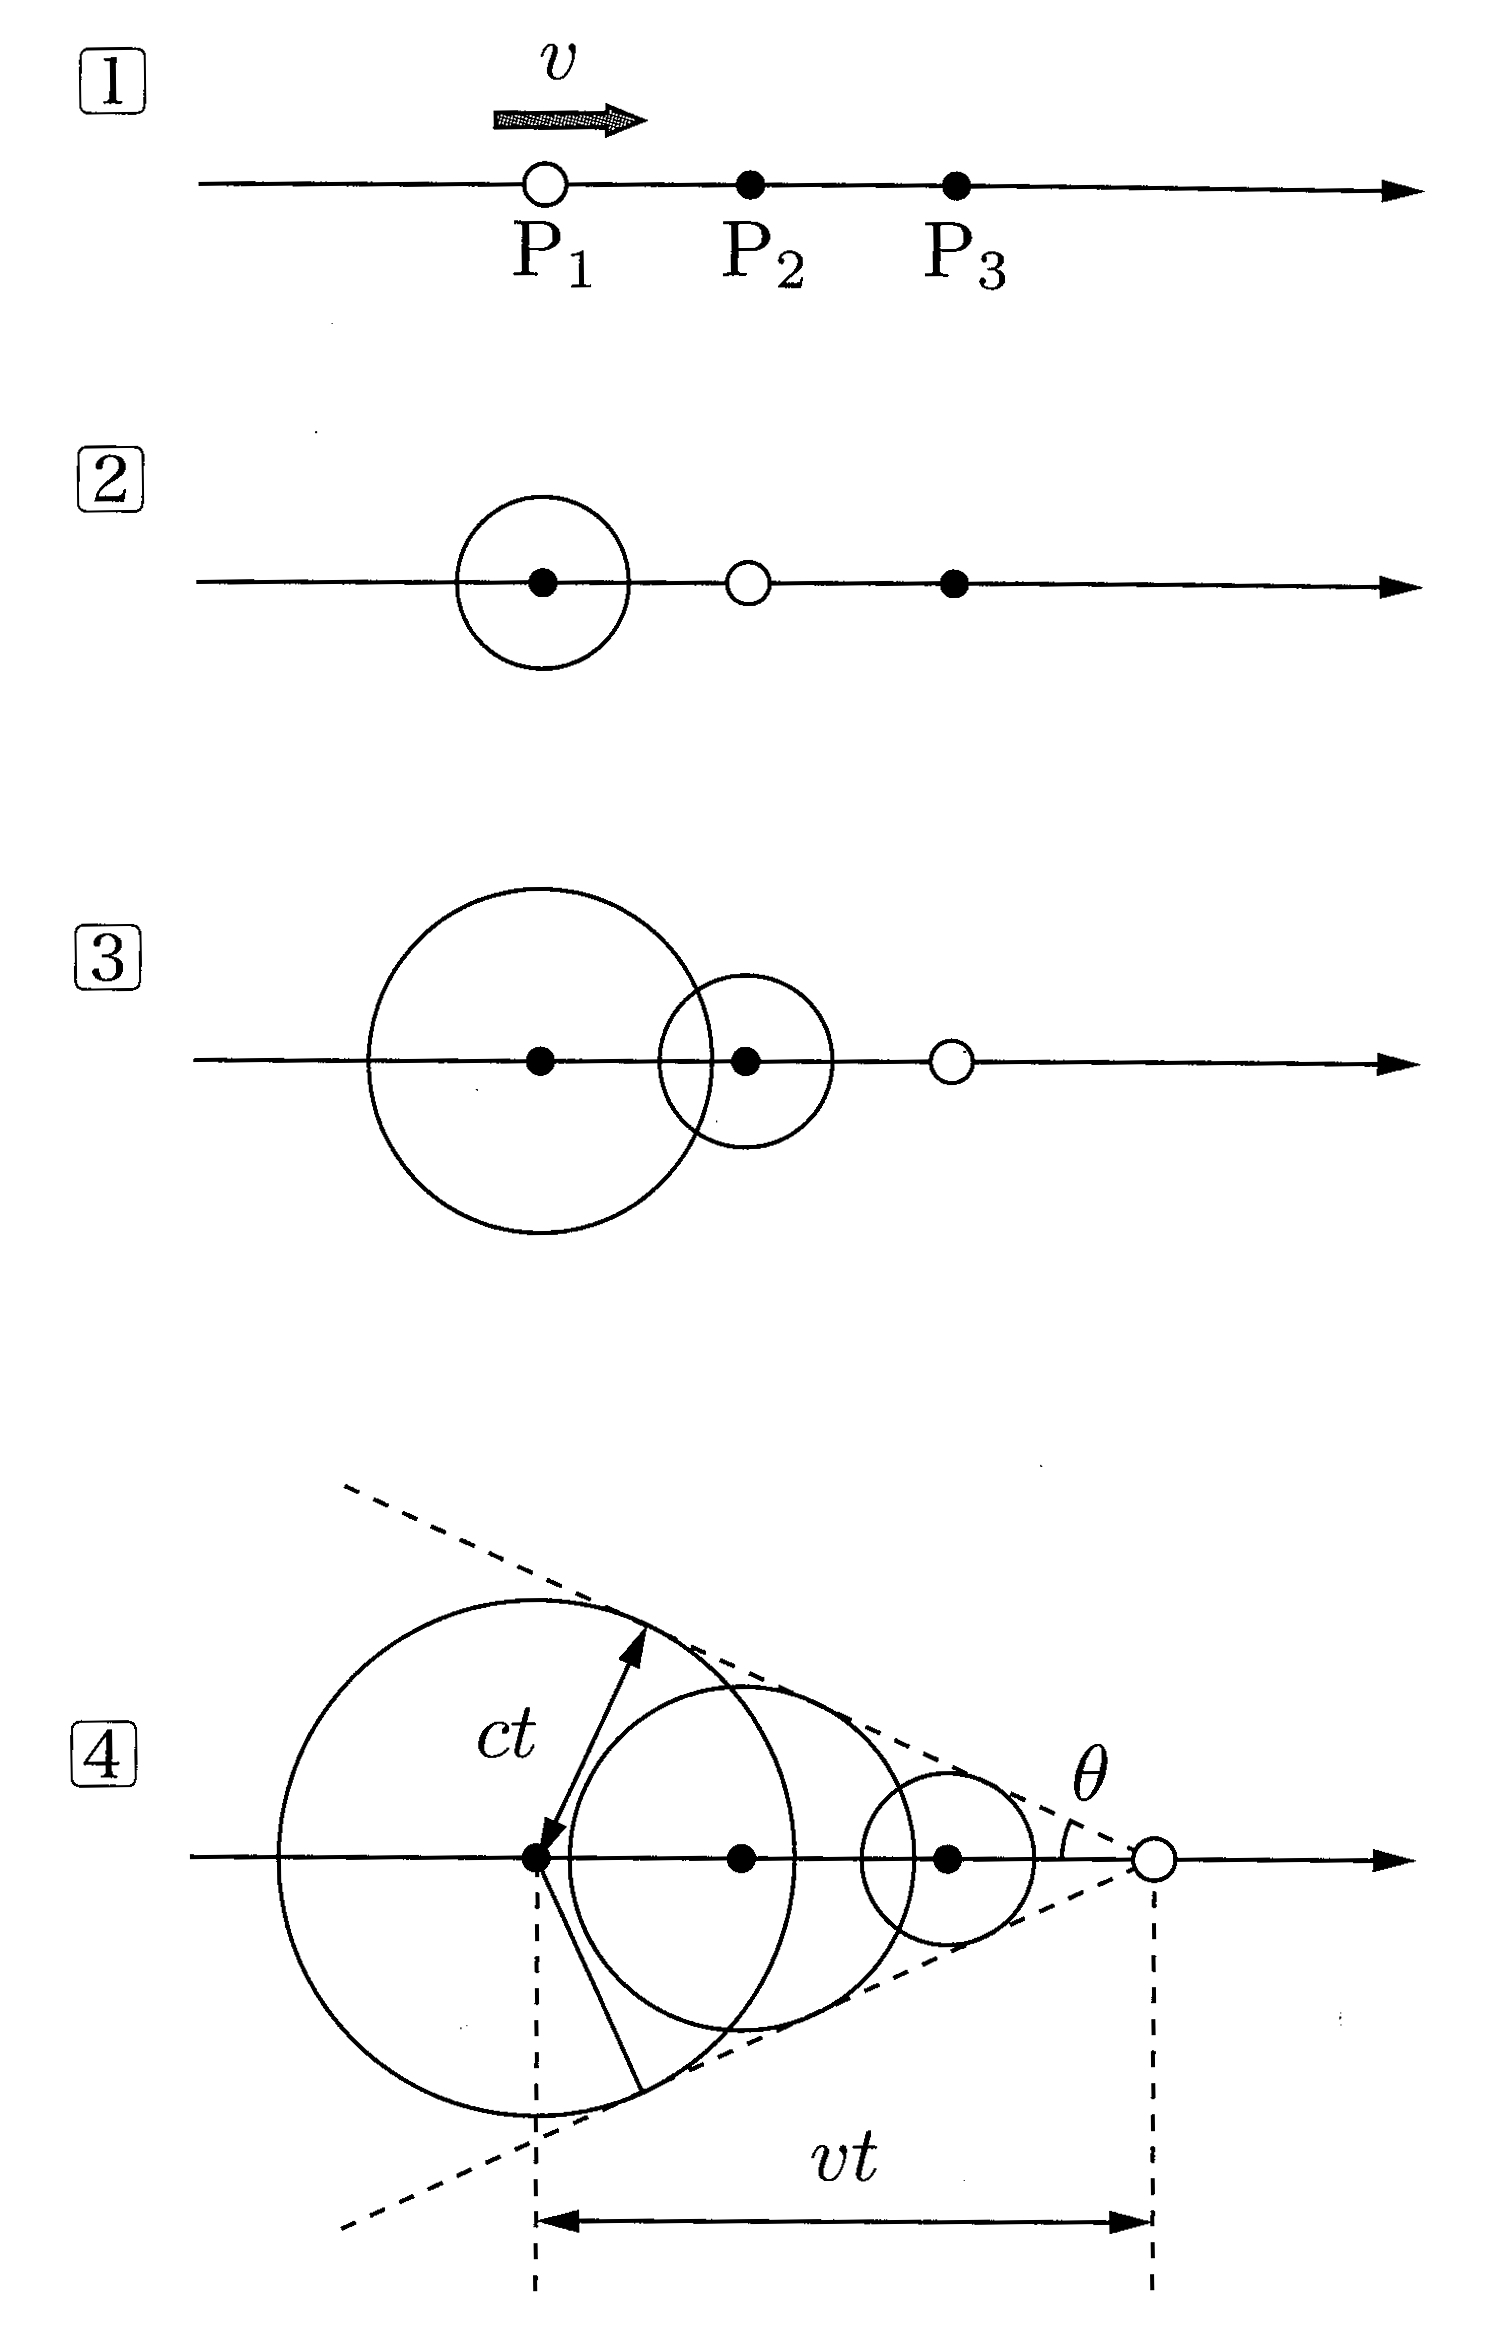
\includegraphics[keepaspectratio,width=65mm]
  {text_p115_fig1.png}
\end{wrapfigure}
音源Sの速さが$v$[m/s]，音速が$c$[m/s]とし，$v>c$の条件が満たされている場合について考えると，図$\fbox{1}$のP$_1$を通過したときに出た音波はP$_1$を中心として同心円上に広がる．
やがてP$_2$に音源は達するが，このときのP$_1$を通過したときに出された音波の波面は図$\fbox{2}$のようになっている．
P$_2$を通過するときに出す音波は通過したときからP$_2$を中心として同心円上に広がっていく．
これを繰り返していくと，各P$_1$，P$_2$，P$_3$などから出た音波は図のような円錐形の波面を作ることになる．
波面上には各時刻に出された球面波が重なり合うため，非常に大きな振幅を持つ波面となる．
このような波を{\bf 衝撃波}という．

P$_1$を通過してから時間$t$[s]だけ経過したときを考えると，衝撃波の半頂角を$\theta$として，図より
\[\sin \theta =\dfrac{c\cdot t}{v\cdot t}=\dfrac{c}{v}\]
という関係が満たされる．
衝撃波においては，波源の進行方向の波源より前方には波は伝わっていかず，波源の後方へ進む波については通常のドップラー効果が観測される．

\vspace{5mm}
 \begin{matome}{衝撃波}
 \hspace{3mm} 波源の速さが波の速さを超えると，波源の進行方向の波源より前方には波は伝わっていかない．\\
 \hspace{3mm} 波源から出る波の波面は波源を頂点とする円錐形をなし，その半頂角$\theta$は$\sin \theta=\dfrac{c}{v}$を満たす．
  \end{matome}
 
\subsection{光速度}
光は真空中において{\bf 高速度}\mbox{\boldmath $c=2.99792458\times 10^8 \fallingdotseq 3.00 \times 10^8$} {\bf [m/s]の速さをもつ横波}であることが知られている．
そのため，波動としての特徴である回折や干渉を起こし，また横波であるために後に述べる偏光といった現象を起こす．
真空中の{\bf 光の速さは光の波長，振動数によらず一定}であることが知られている．

 \begin{matome}{光速度}
 \hspace{3mm} $c\fallingdotseq 3.00\times 10^8$[m/s]\hspace{5mm} 波長・振動数によらない
 \end{matome}

\subsection{光の屈折}
ある媒質を伝わる光波が別の媒質に入射するとき，光波はその一部が境界面で反射し，残りは屈折してもう一方の媒質に入る．
このとき，境界面に対して垂直に立てた法線に対する角度をそれぞれ{\bf 入射角，屈折角}という．

\begin{wrapfigure}[8]{r}[5mm]{60mm}
  \centering
  \vspace{-5mm}
  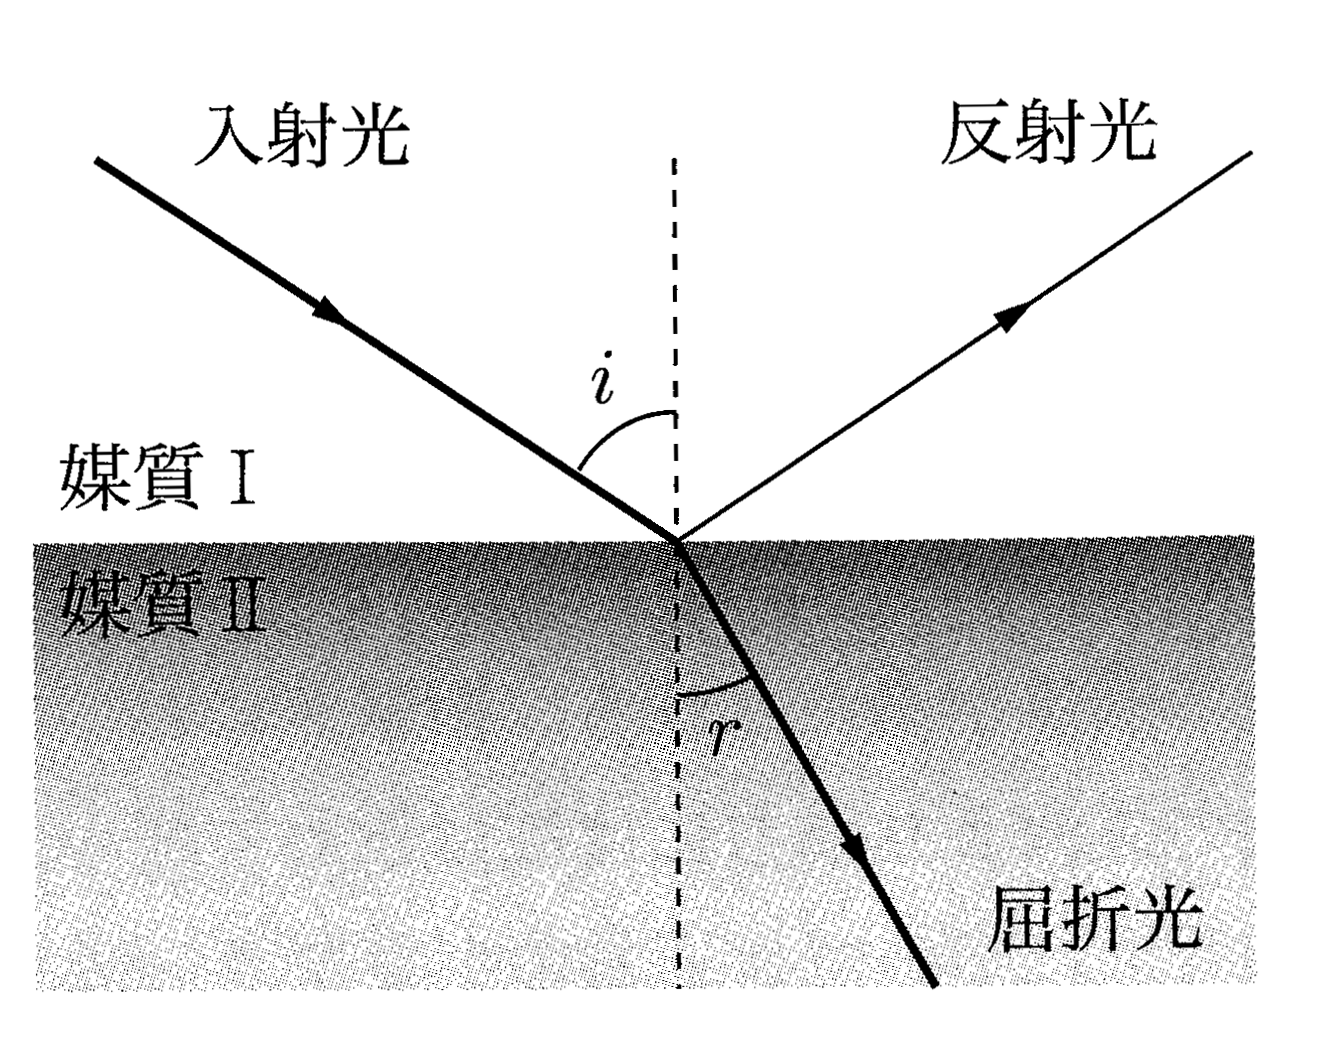
\includegraphics[keepaspectratio,width=60mm]
  {text_p116_fig1.png}
\end{wrapfigure}
入射角を$i$，屈折角を$r$とし，媒質I，媒質II中の光の速さ，波長をそれぞれ$c_1,c_2$[m/s]，$\lambda_1,\lambda_2$[m]とすると，
\[\mbox{\boldmath $\dfrac{\sin i}{\sin r} =\dfrac{c_1}{c_2}= \dfrac{\lambda_1}{\lambda_2} =n_{12} $}\hspace{5mm} \cdots \cdots （☆）\]
が成立する．
この比の値は入射角$i$に依存しない．
$n_{12}$を{\bf 媒質Iに対する媒質IIの屈折率（相対屈折率）}という．
また，{\bf 屈折の前後で振動数は変化しない．}
この式は光波に限らず，波動全般について成立する．

特に光波の場合は，真空に対する媒質の屈折率をその媒質の{\bf 絶対屈折率}という．
媒質I，媒質IIの絶対屈折率を$n_1,n_2$，真空中の光の速さを$c$[m/s]とすると，屈折率の定義式より
\[ n_1=\dfrac{c}{c_1},\hspace{5mm}n_2=\dfrac{c}{c_2}\]
が成立する．
$n_{12},n_1,n_2$の間には$n_{12}=\dfrac{n_2}{n_1}$が成立する．
絶対屈折率$n$は{\bf 真空の場合は1，それ以外は1より大きくなる}と考えてよい．

なお，$n_1,n_2$を用いると，☆式は次の形に書き直すことができる．
\[\mbox{\boldmath $ n_1\sin i=n_2\sin r ,\hspace{5mm} n_1c_1=n_2c_2 ,\hspace{5mm} n_1\lambda_1=n_2\lambda_2$}\]

 \begin{matome}{屈折の法則}
 \hspace{3mm} $n_1\sin i=n_2\sin r ,\hspace{5mm} n_1c_1=n_2c_2 ,\hspace{5mm} n_1\lambda_1=n_2\lambda_2$\\
 屈折の前後で波の振動数は不変．
 \end{matome}

屈折率の大きなものから小さなものへ光が進む場合は入射角$i$よりも屈折角$r$の方が大きくなるため，入射角がある値$\theta_0$を越えると屈折光は存在できなくなり，すべての光が反射される．
これを全反射といい，角度$\theta_0$を{\bf 臨界角}という．

\begin{wrapfigure}[6]{r}[5mm]{60mm}
  \centering
  \vspace{-5mm}
  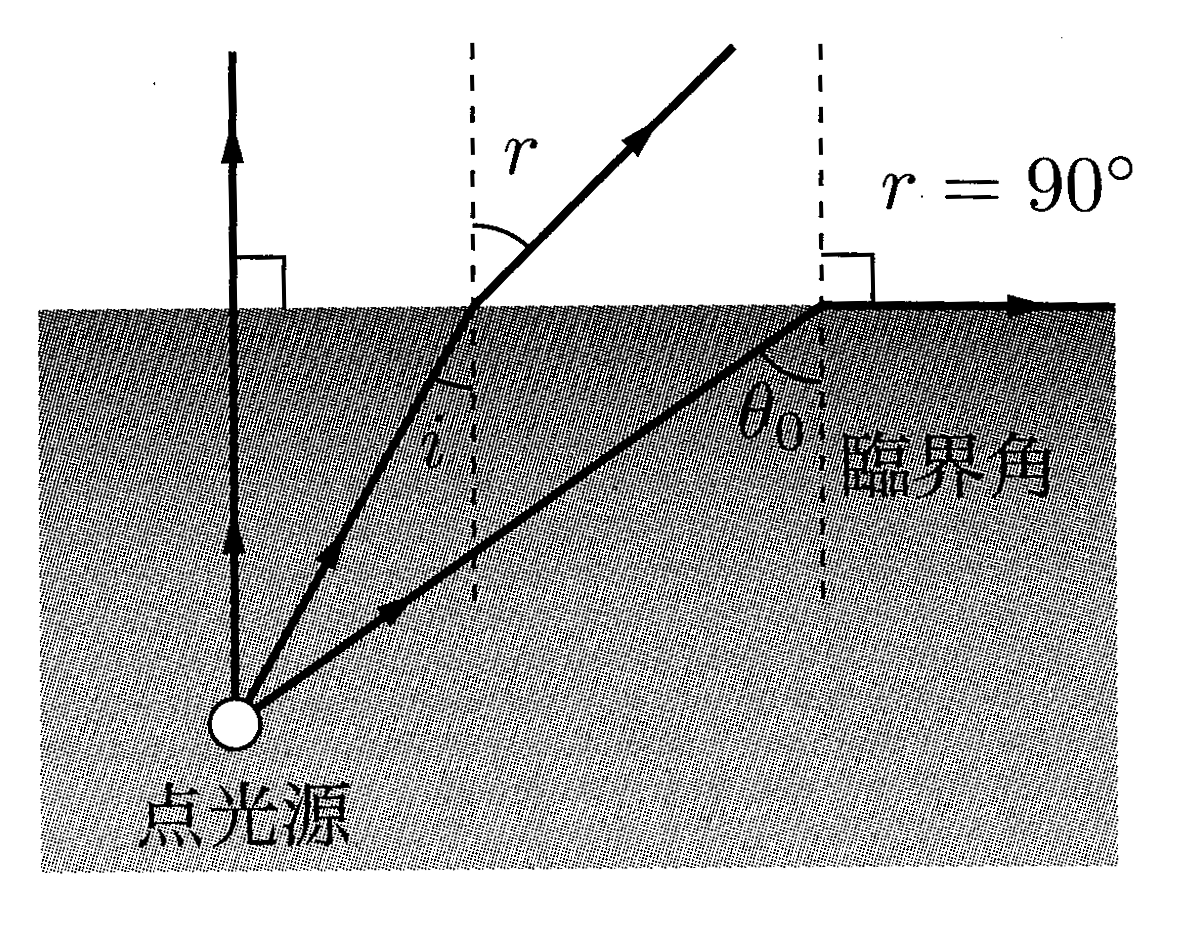
\includegraphics[keepaspectratio,width=60mm]
  {text_p117_fig1.png}
\end{wrapfigure}
簡単のため，右図のように屈折率$n$の媒質中の点光源から出た光が真空中へと出ていく場合について考える．
屈折の法則から$\sin r=n\sin i$となるが，\mbox{\boldmath $\sin r=n\sin i >1$}{\bf となると屈折光は存在できない．}
すなわち，
\[\mbox{\boldmath $ \sin i>\dfrac{1}{n}$}\]
なる入射角$i$の光は全反射することになる．
よって，臨界角を$\theta_0$とすると，
\[\sin \theta_0 =\dfrac{1}{n}\]
が成立する．
{\bf 臨界角を求めるには，屈折の法則において屈折角を直角と置けばよい．}

\subsection{ホイヘンスの原理と屈折の法則}
波が平面上もしくは空間中を伝わっていくとき，ある瞬間に波の同位相の点を連ねていくと，一つの曲線もしくは曲面ができる．
この面を波面といい，この波面が平面である波を{\bf 平面波}，球面になる波を{\bf 球面波}という．
波面は常に波の進行方向に対して垂直になっている．

\begin{wrapfigure}[13]{r}[5mm]{100mm}
  \centering
  \vspace{-5mm}
  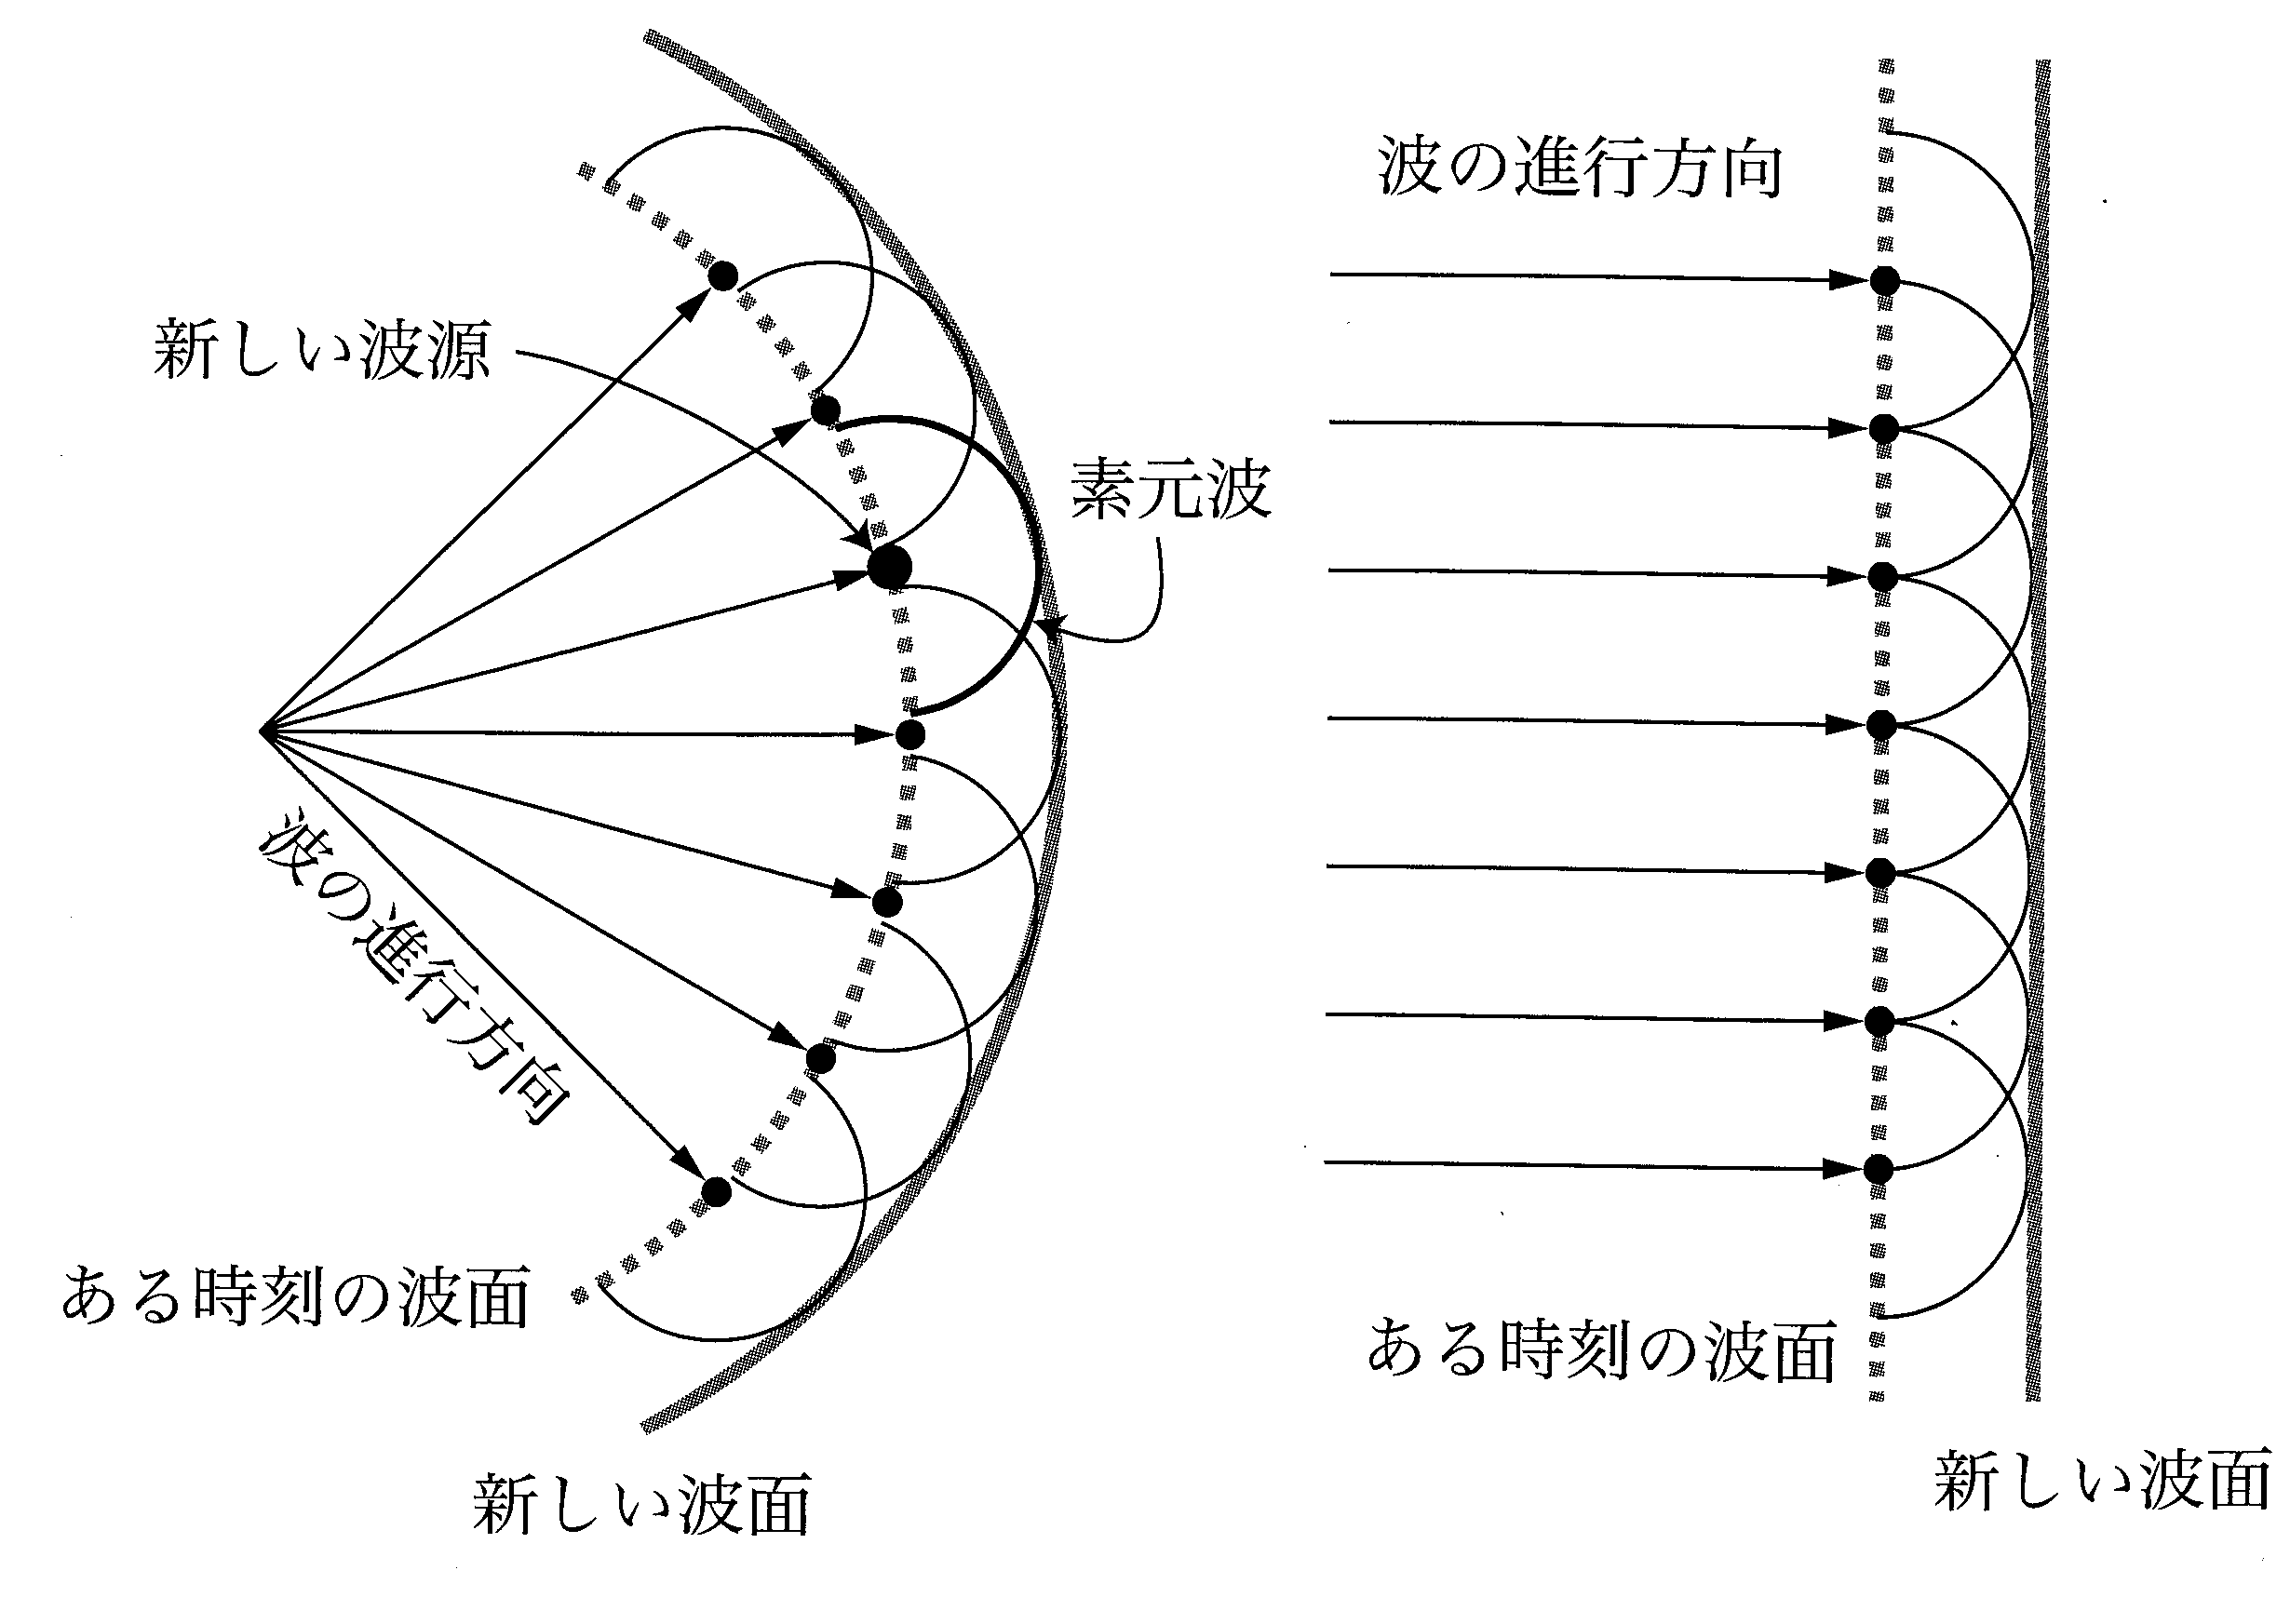
\includegraphics[keepaspectratio,width=100mm]
  {text_p118_fig1.png}
\end{wrapfigure}
波面が次の瞬間にどのように広がっていくかは明らかなことも多いが，一般的には次に述べる{\bf ホイヘンスの原理}に従うことが経験的に知られている．
波が届いた媒質の点は波と同じ振動数で振動を始める．
そのため，これらの点は新たな波源とみなすことができる．
ある波面が次の瞬間にどのような波面になるかは，波面上の各点が新たな波源となって出す球面波（これを{\bf 素元波}という）がどのような曲面を形成するかを考えればよい．
多数の素元波のすべてに接する曲面（包絡面）のうち，波の進行方向側にできるものが次の瞬間の波面となる．
これを{\bf ホイヘンスの原理}といい，これを用いると波の反射，屈折，回折現象を説明することができる．

 \begin{matome}{ホイヘンスの原理}
 \hspace{3mm} 波動がある瞬間に作る波面の各点から出る無数の素元波の包絡面が次の瞬間の波面となる．
  \end{matome}
 
 \begin{wrapfigure}[7]{r}[5mm]{60mm}
  \centering
  \vspace{-5mm}
  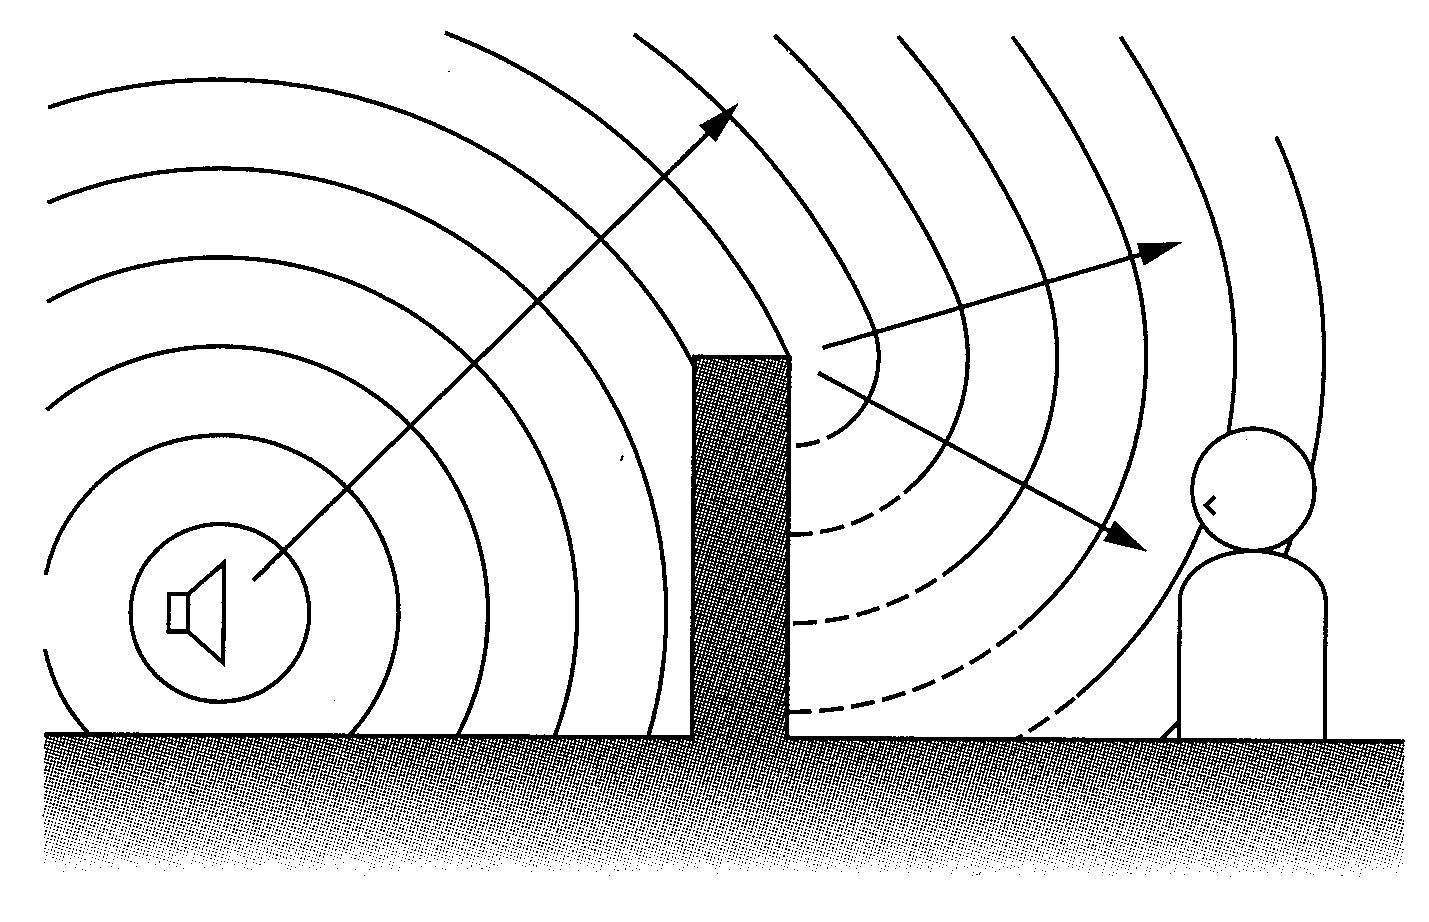
\includegraphics[keepaspectratio,width=60mm]
  {text_p118_fig2.png}
\end{wrapfigure}
 波が障害物に当たったとき，幾何学的には影となる部分にも実際には若干の波が回り込むことが知られており，これを{\bf 波の回折}といい，回り込んだ波を{\bf 回折波}という．
 
 回折が顕著に起こるか否かは障害物やすき間の大きさと波の波長の大小関係によって決まる．
 すなわち，{\bf すき間などの大きさに比べて十分に大きい波長を持つ波は回折が顕著であり，影の部分に回り込む程度が大きい．}
 逆に，すき間などの大きさに比べて小さい波長を持つ波は回折しにくいことが知られており，これはホイヘンスの原理によって説明できることが知られている．
 
  \begin{figure}[h]
\begin{center}
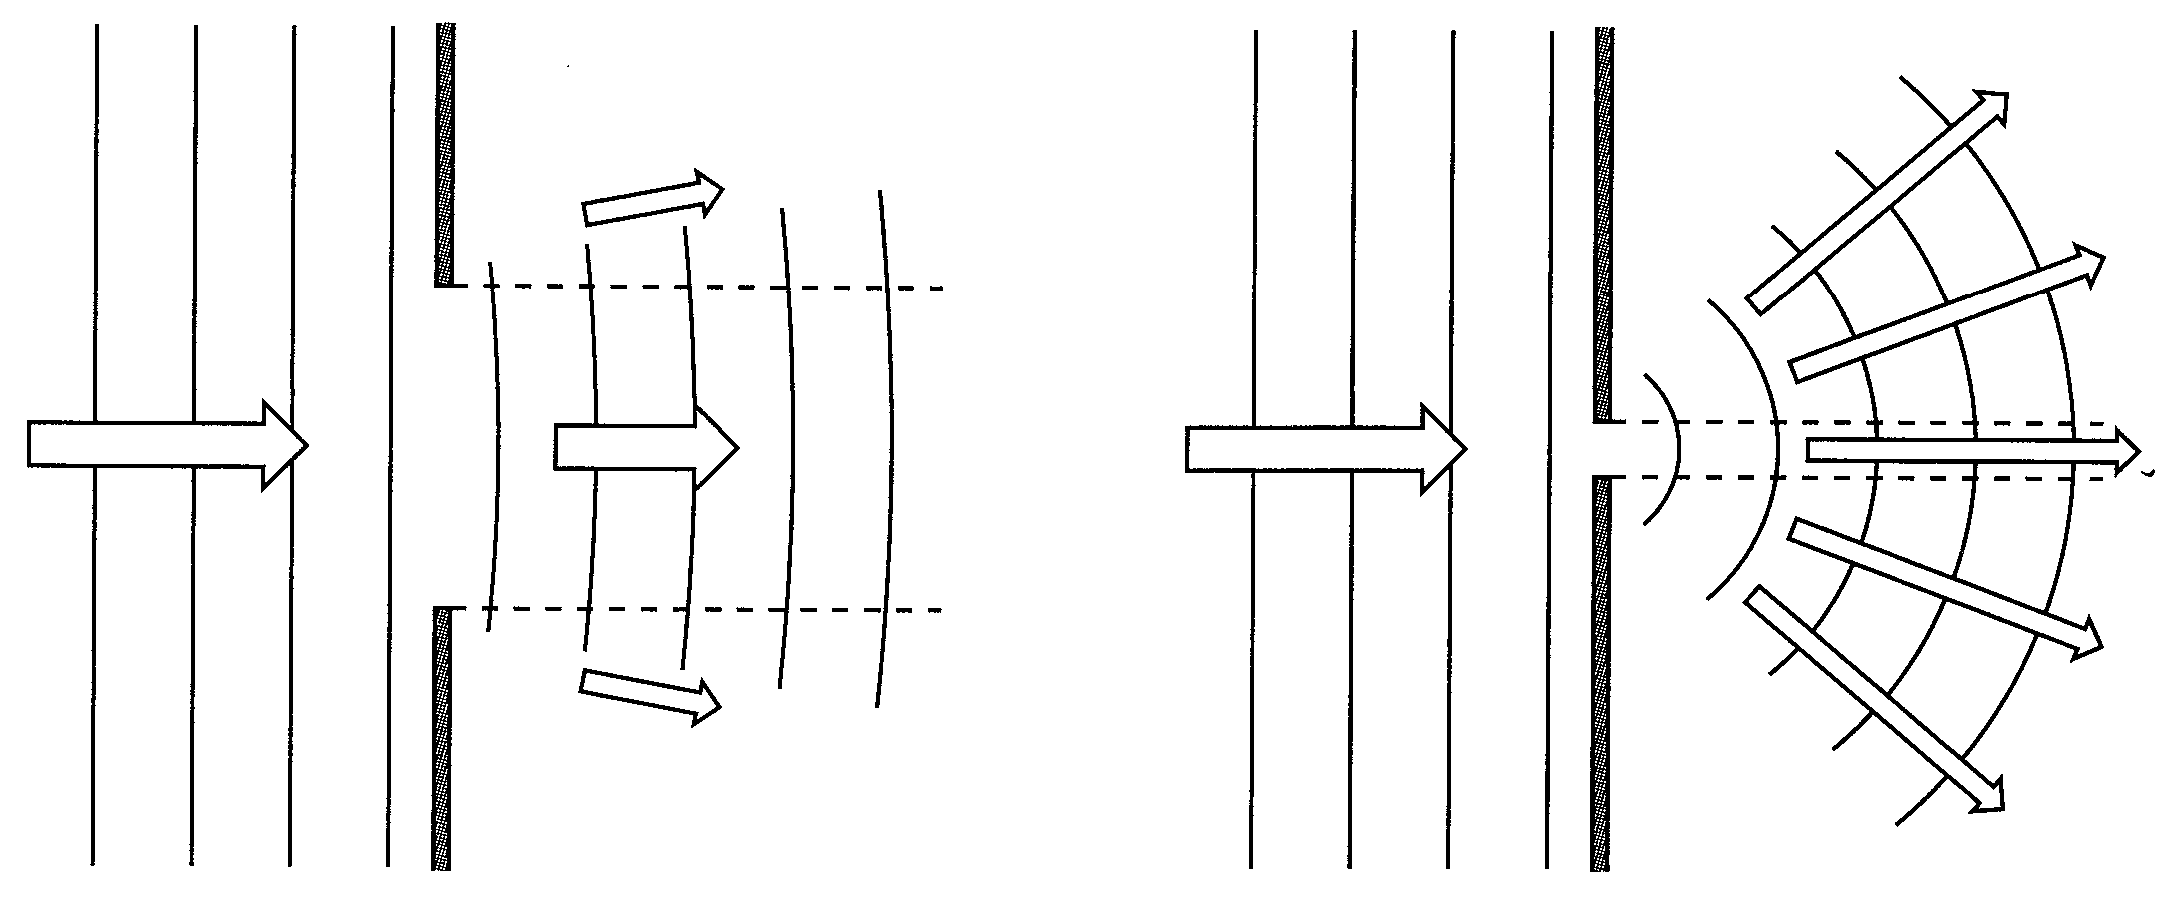
\includegraphics[width=110mm]{text_p118_fig3.png}
\end{center}
\end{figure}
  \vspace{40mm}
  \begin{matome}{回折現象}
 \hspace{3mm} 波の波長が障害物やすき間の大きさに比べて同程度より大きくなると，波の回折が顕著となり，波は幾何学的に影となる部分によく回り込むようになる．
  \end{matome}
  
  
\begin{wrapfigure}[10]{r}[5mm]{90mm}
  \centering
  \vspace{-5mm}
  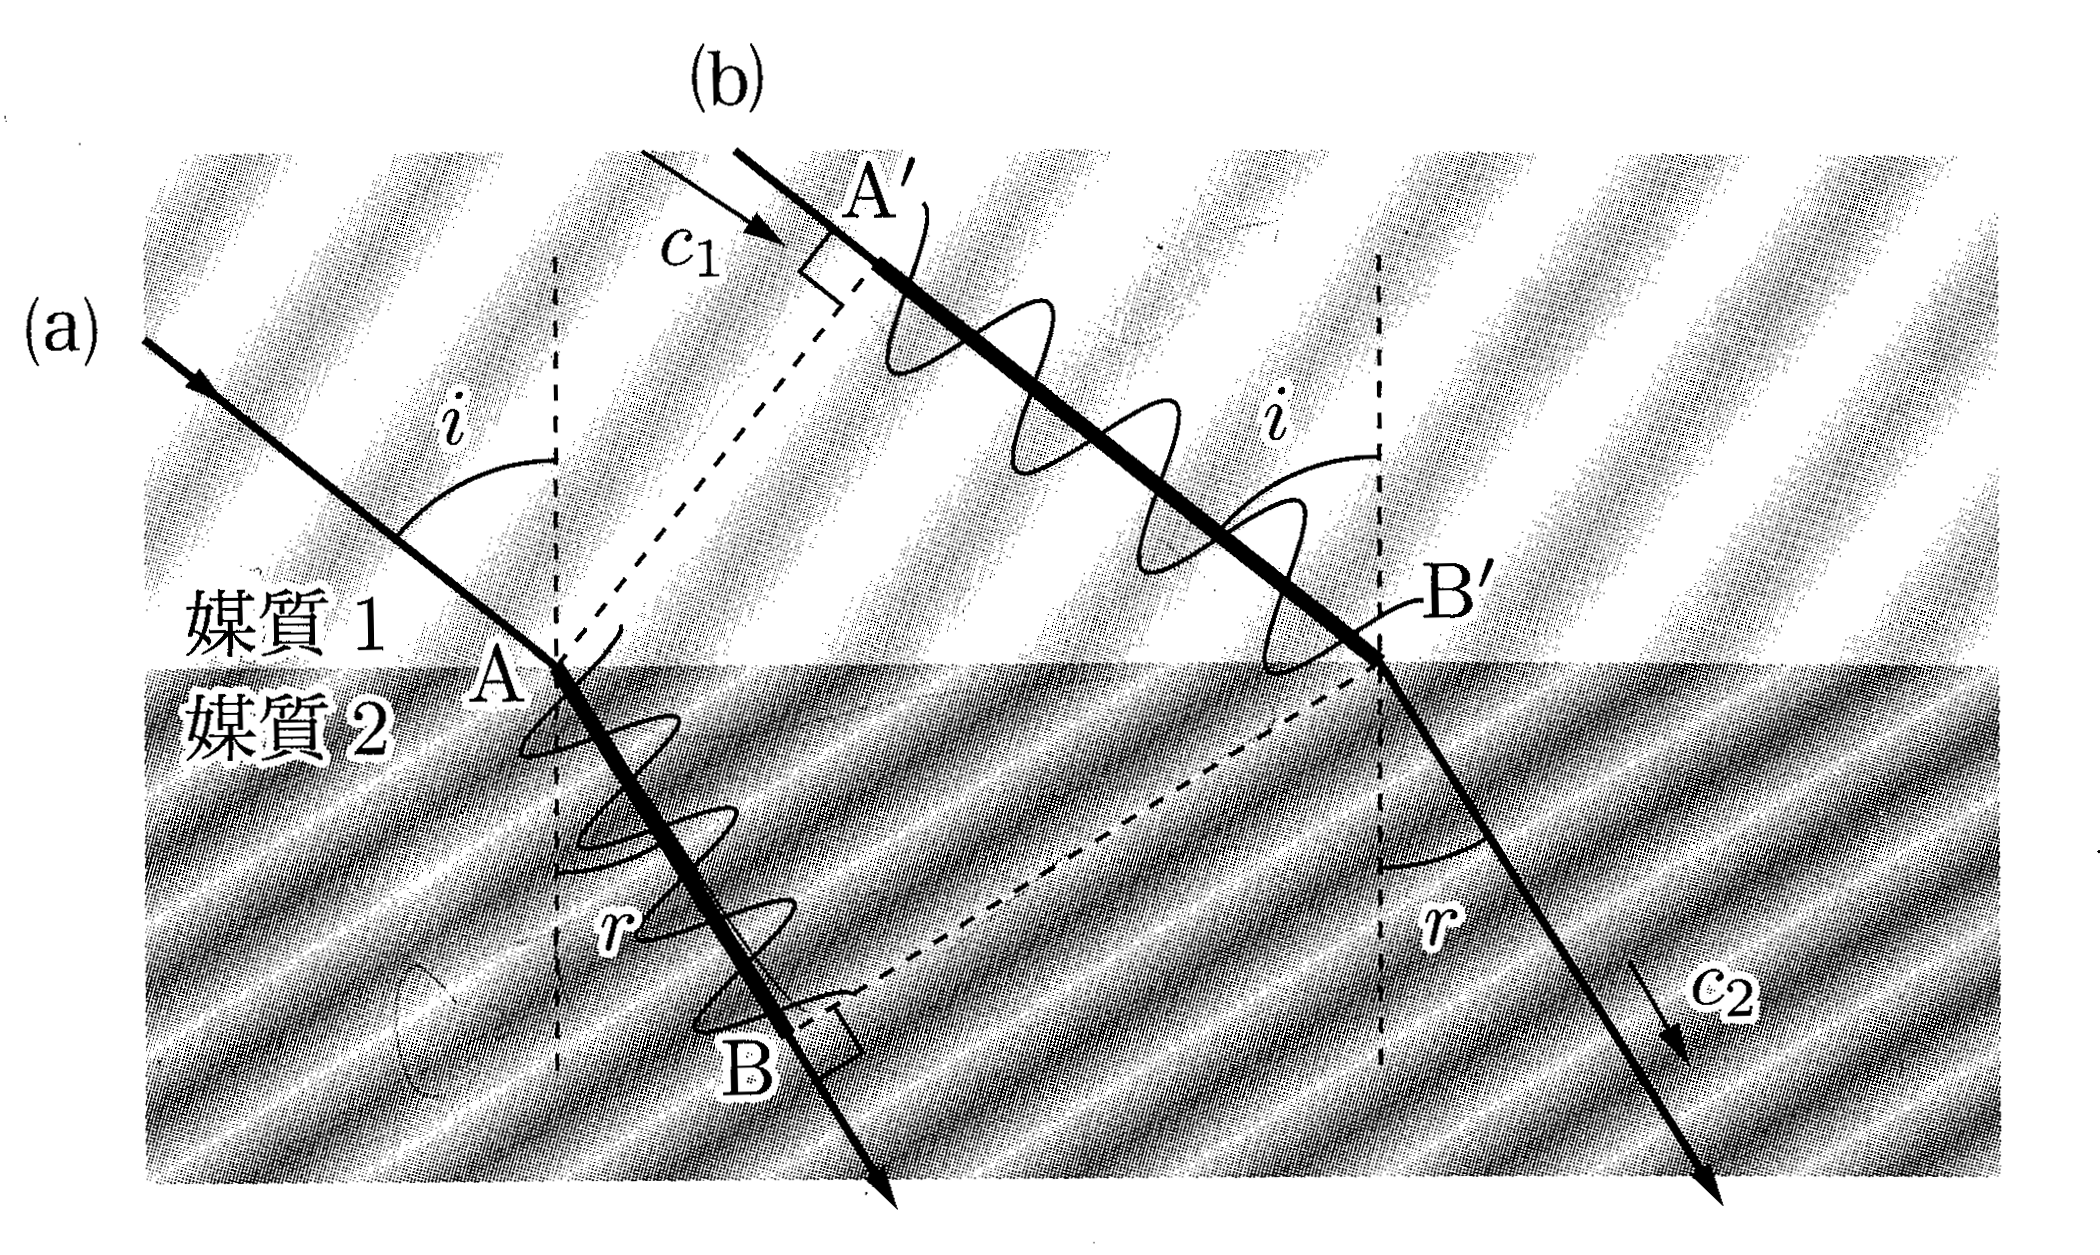
\includegraphics[keepaspectratio,width=90mm]
  {text_p119_fig1.png}
\end{wrapfigure}
以上で述べたホイヘンスの原理を用いると，屈折の法則の公式を以下のようにして導くことができる．
図のように，媒質Iから媒質IIへ向けて位相の揃った平面波が入射角$i$で入射し，屈折角$r$で屈折していく場合を考えよう．
波面は波の進行方向に対して垂直であるから，図のA,A$^\prime$は同一波面上に，また屈折した後のB,B$^\prime$も同一波面上にある．
すなわち，A,A$^\prime$は同位相であり，B,B$^\prime$も同位相であるから，(a)のルートを通る波がAからBへ進む間に，(b)のルートを通る波はA$^\prime$からB$^\prime$へ進んでいるはずである．

ここで，各媒質中の波の速さおよび波長をそれぞれ$c_1,c_2$[m/s]，$\lambda_1,\lambda_2$[m]とする．
AからBへ波が進むのにかかる時間（=A$^\prime$からB$^\prime$へ波が進むのにかかる時間）を$T$[s]とすると，波の進行距離および幾何学的関係より，
\[\overline{{\rm A}^\prime {\rm B}^\prime} =c_1T,\hspace{4mm} \overline{{\rm AB} } =c_2T,\hspace{4mm} \overline{{\rm A}^\prime {\rm B}^\prime} =\overline{{\rm AB}^\prime}\sin i ,\hspace{4mm} \overline{{\rm AB}} = \overline{ {\rm AB}^\prime}\sin r\]
である．
これらの式より，
\[\dfrac{\overline{{\rm A}^\prime {\rm B}^\prime}}{\overline{{\rm AB} }} =\dfrac{\overline{{\rm AB}^\prime}\sin i }{ \overline{ {\rm AB}^\prime}\sin r} =\dfrac{c_1T}{c_2T}\]
となるので，
\[\dfrac{\sin i}{\sin r}=\dfrac{c_1}{c_2}\]
なる屈折の法則が成立する．
また，屈折の前後で波の振動数$f$は不変であるから，
\[ \dfrac{\sin i}{\sin r}=\dfrac{c_1}{c_2}=\dfrac{c_1/f}{c_2/f}=\dfrac{\lambda_1}{\lambda_2}\]
となる．

\newpage

\begin{figure}[h]
\begin{center}
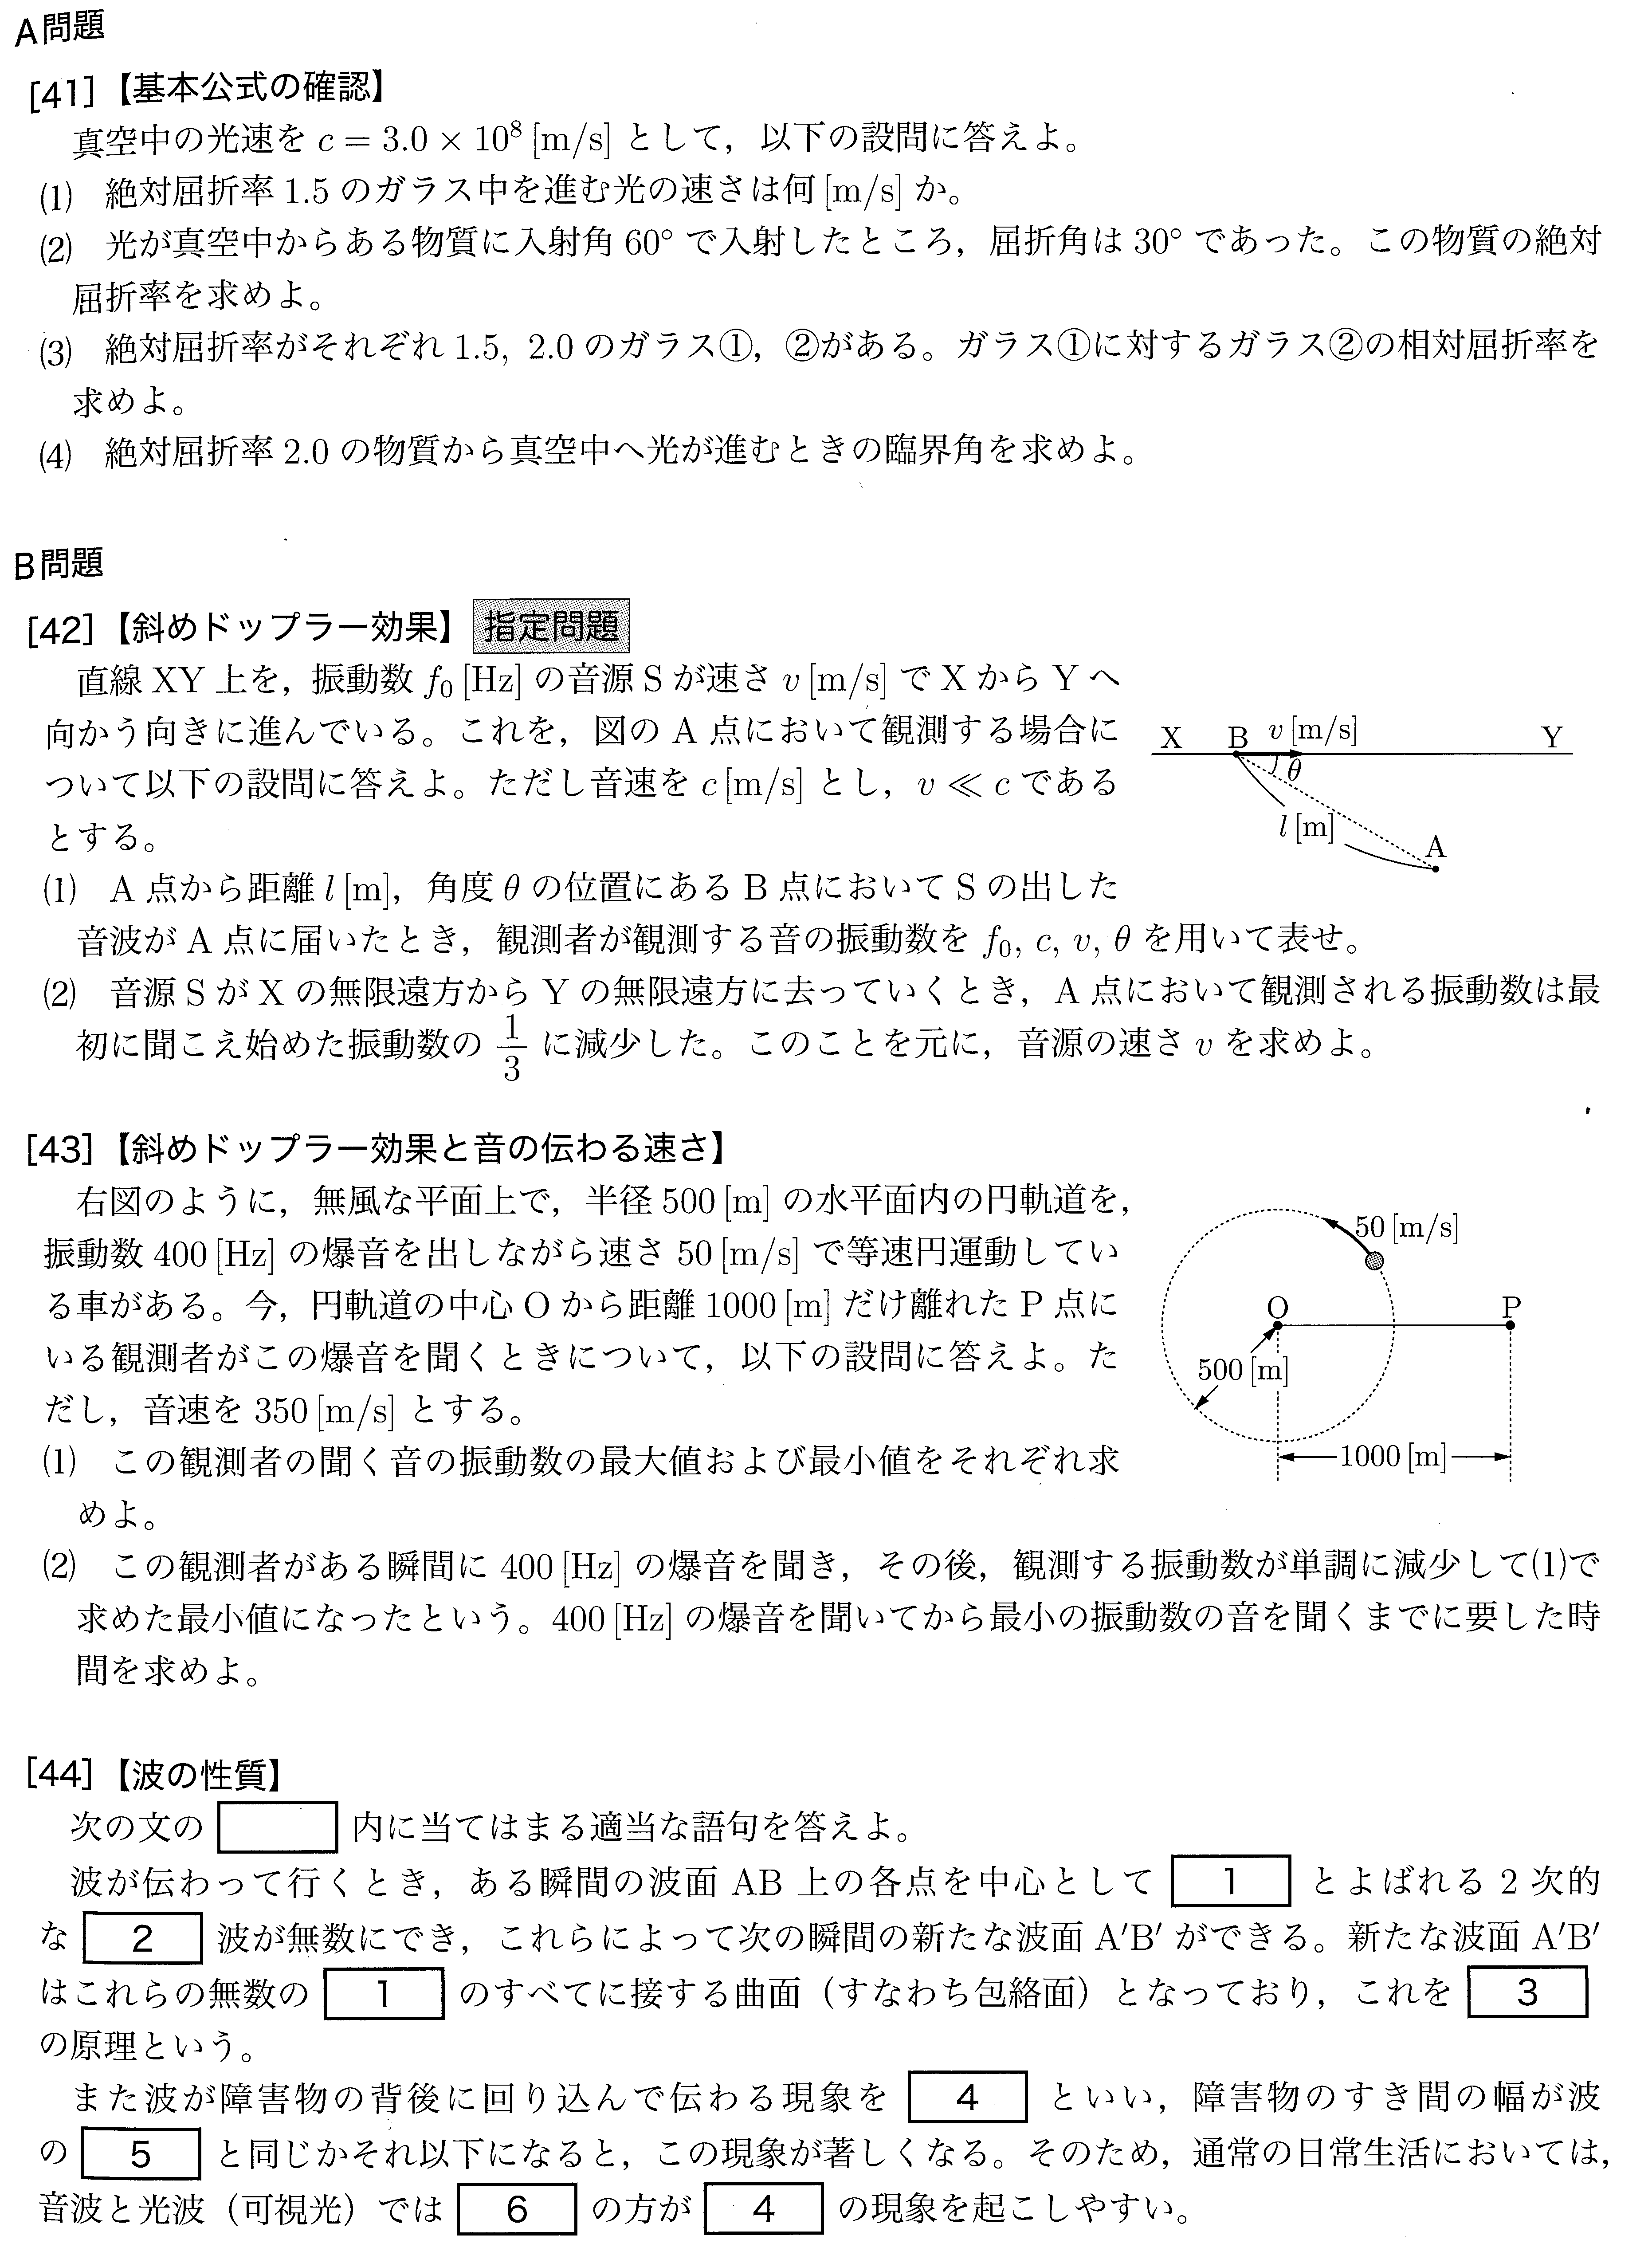
\includegraphics[width=170mm]{prob_p61.png}
\vspace{150mm}
\end{center}
\end{figure}

\newpage

\begin{figure}[h]
\begin{center}
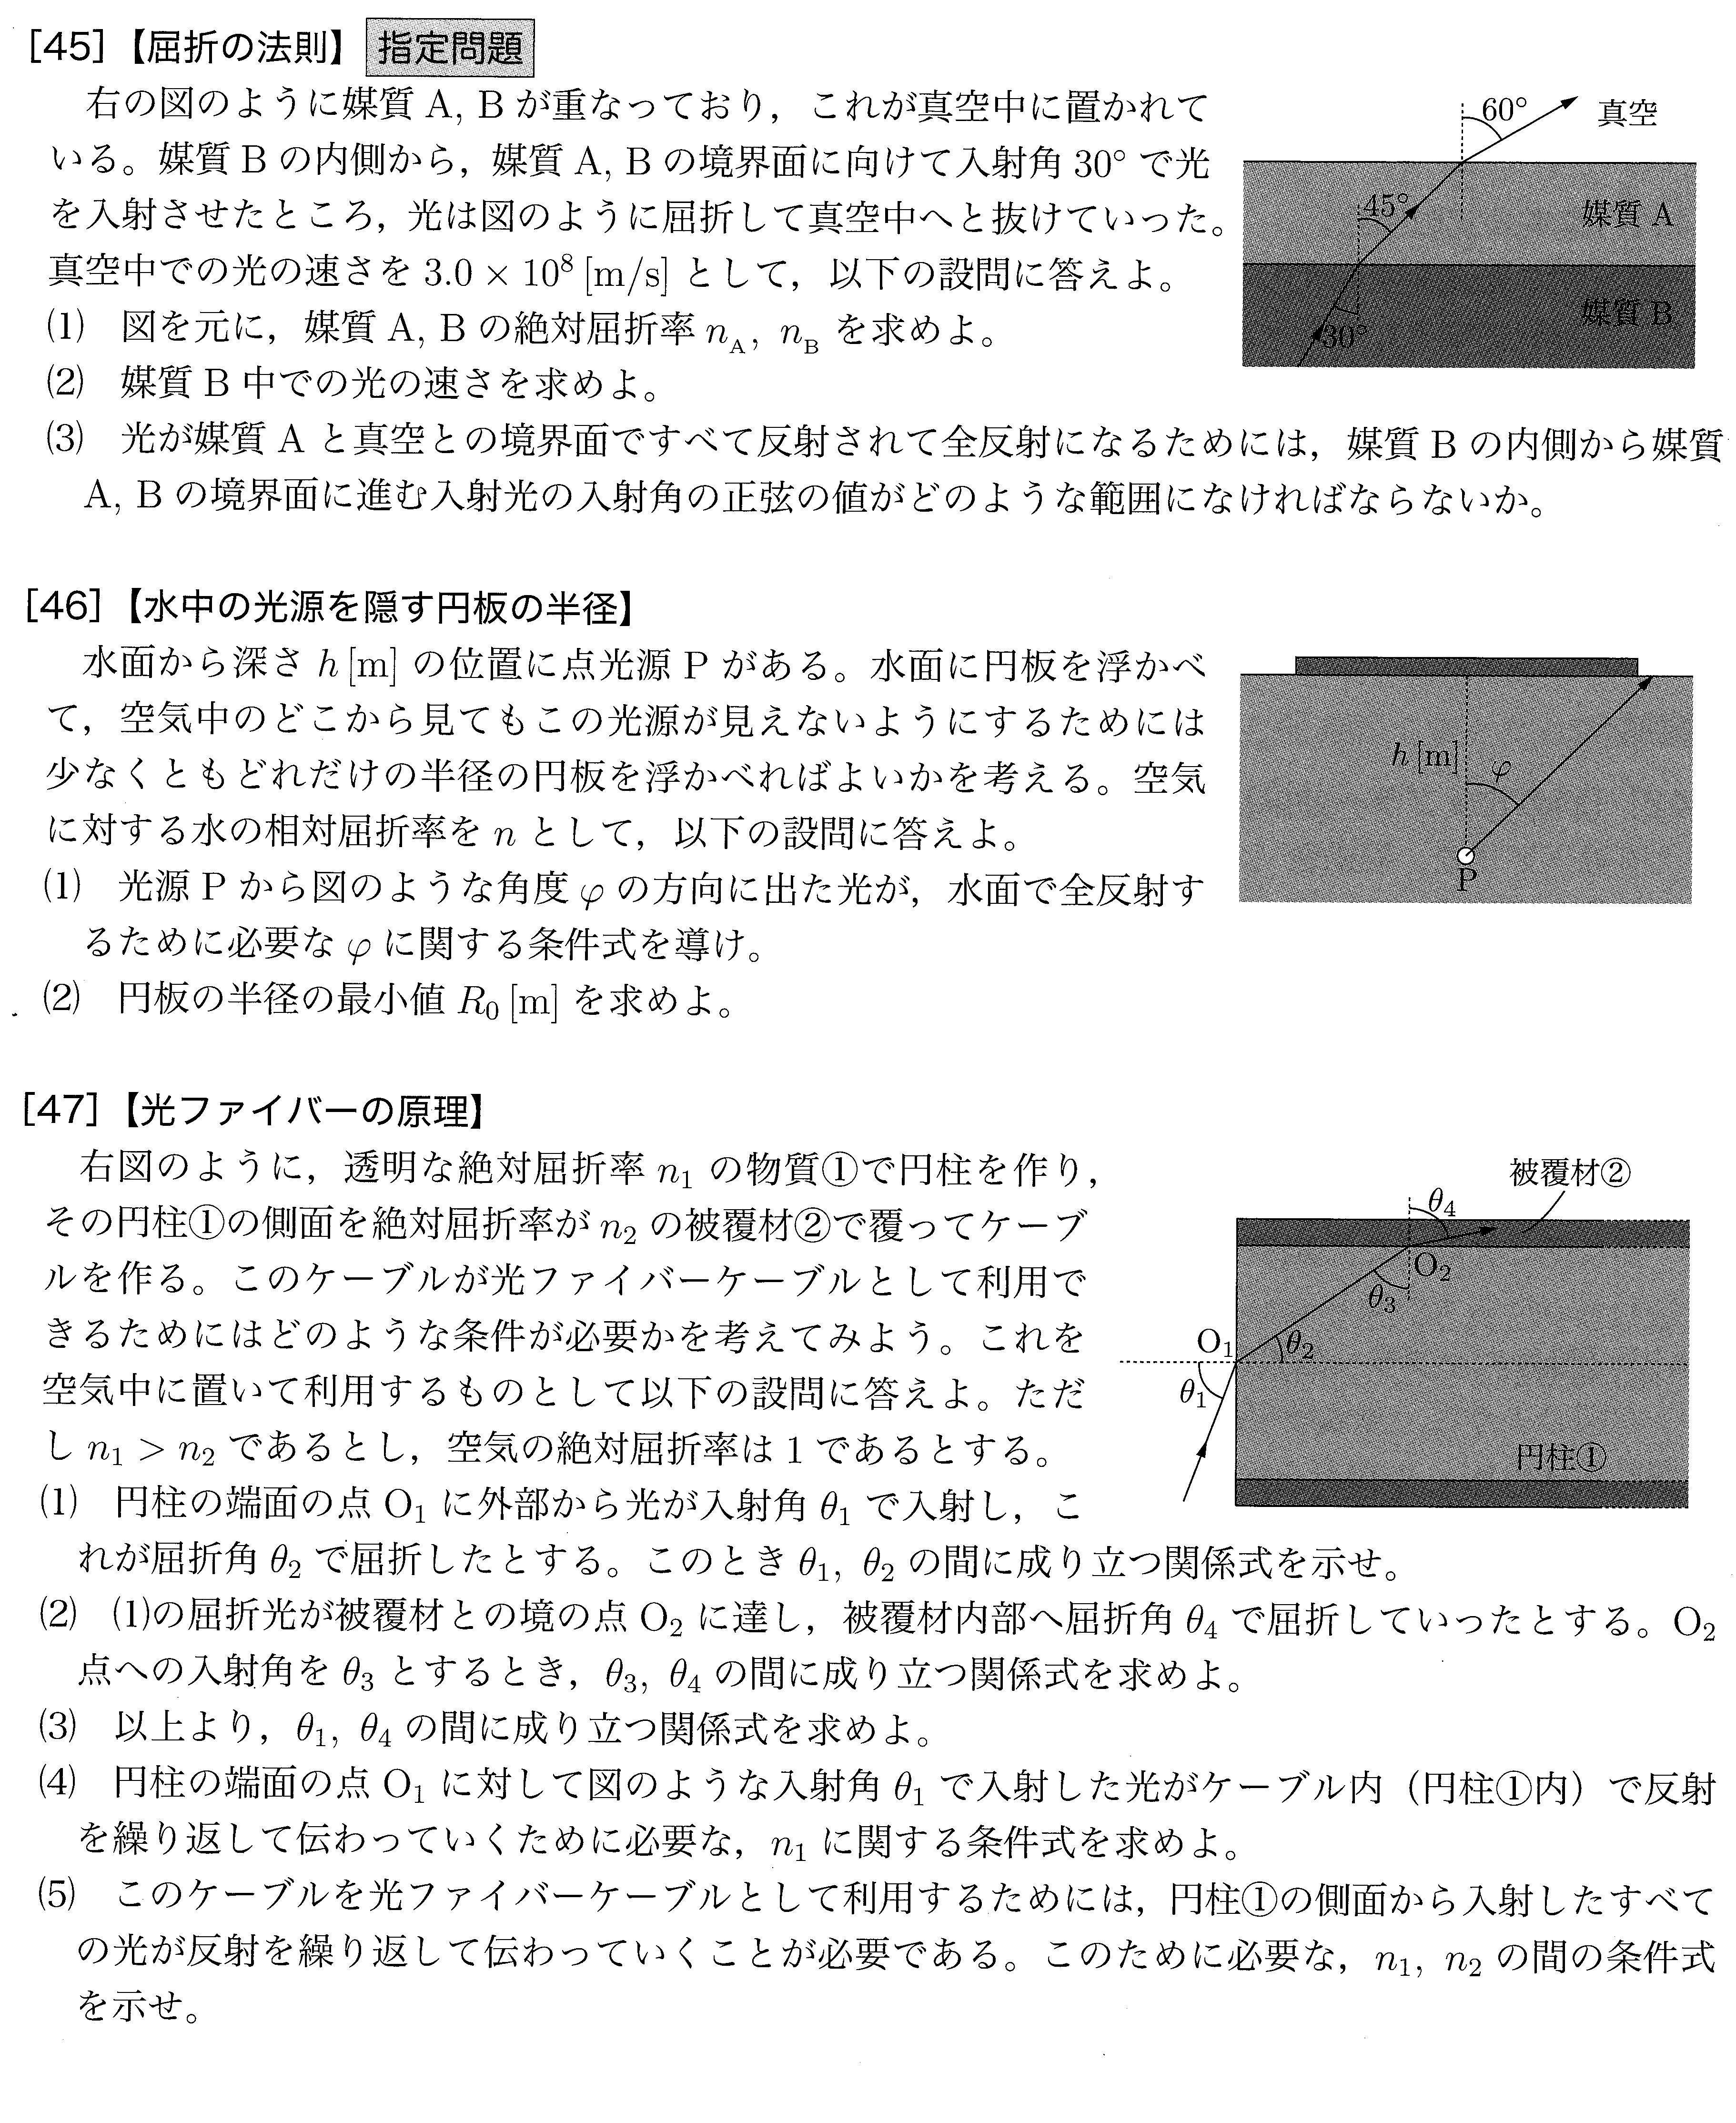
\includegraphics[width=170mm]{prob_p62.png}
\vspace{150mm}
\end{center}
\end{figure}

\newpage

\begin{figure}[h]
\begin{center}
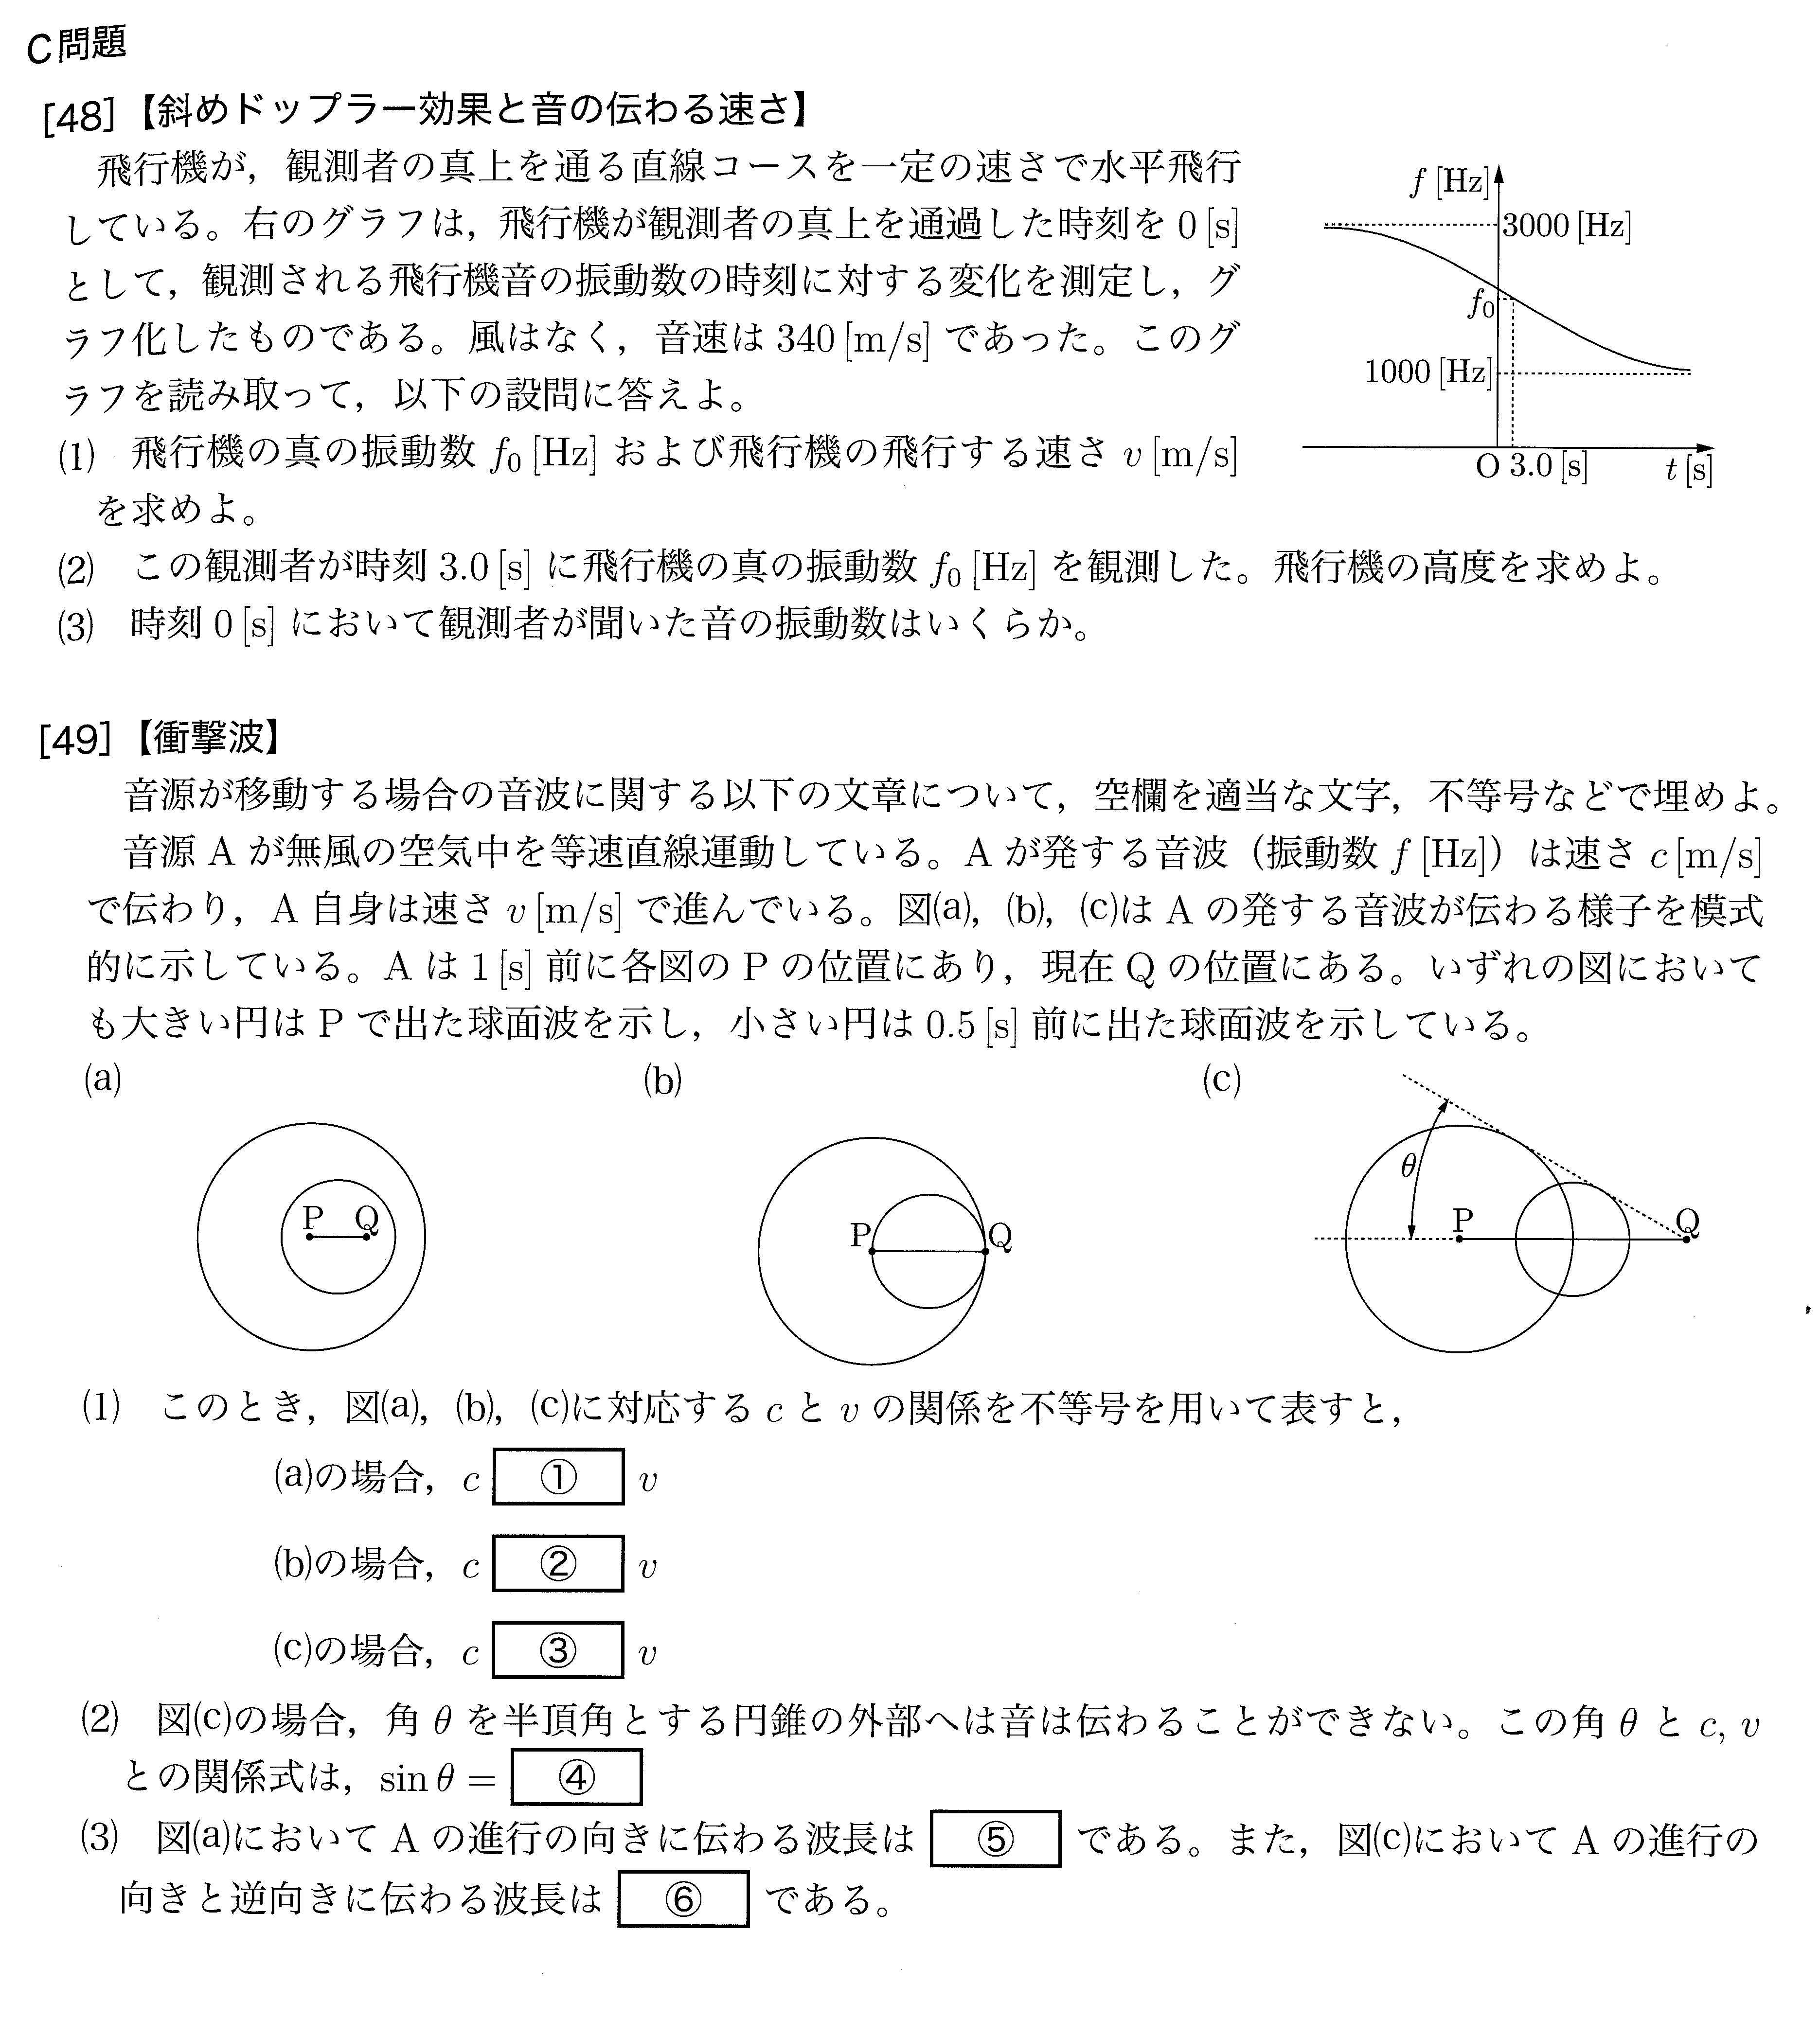
\includegraphics[width=170mm]{prob_p63.png}
\vspace{150mm}
\end{center}
\end{figure}

\newpage

\begin{figure}[h]
\begin{center}
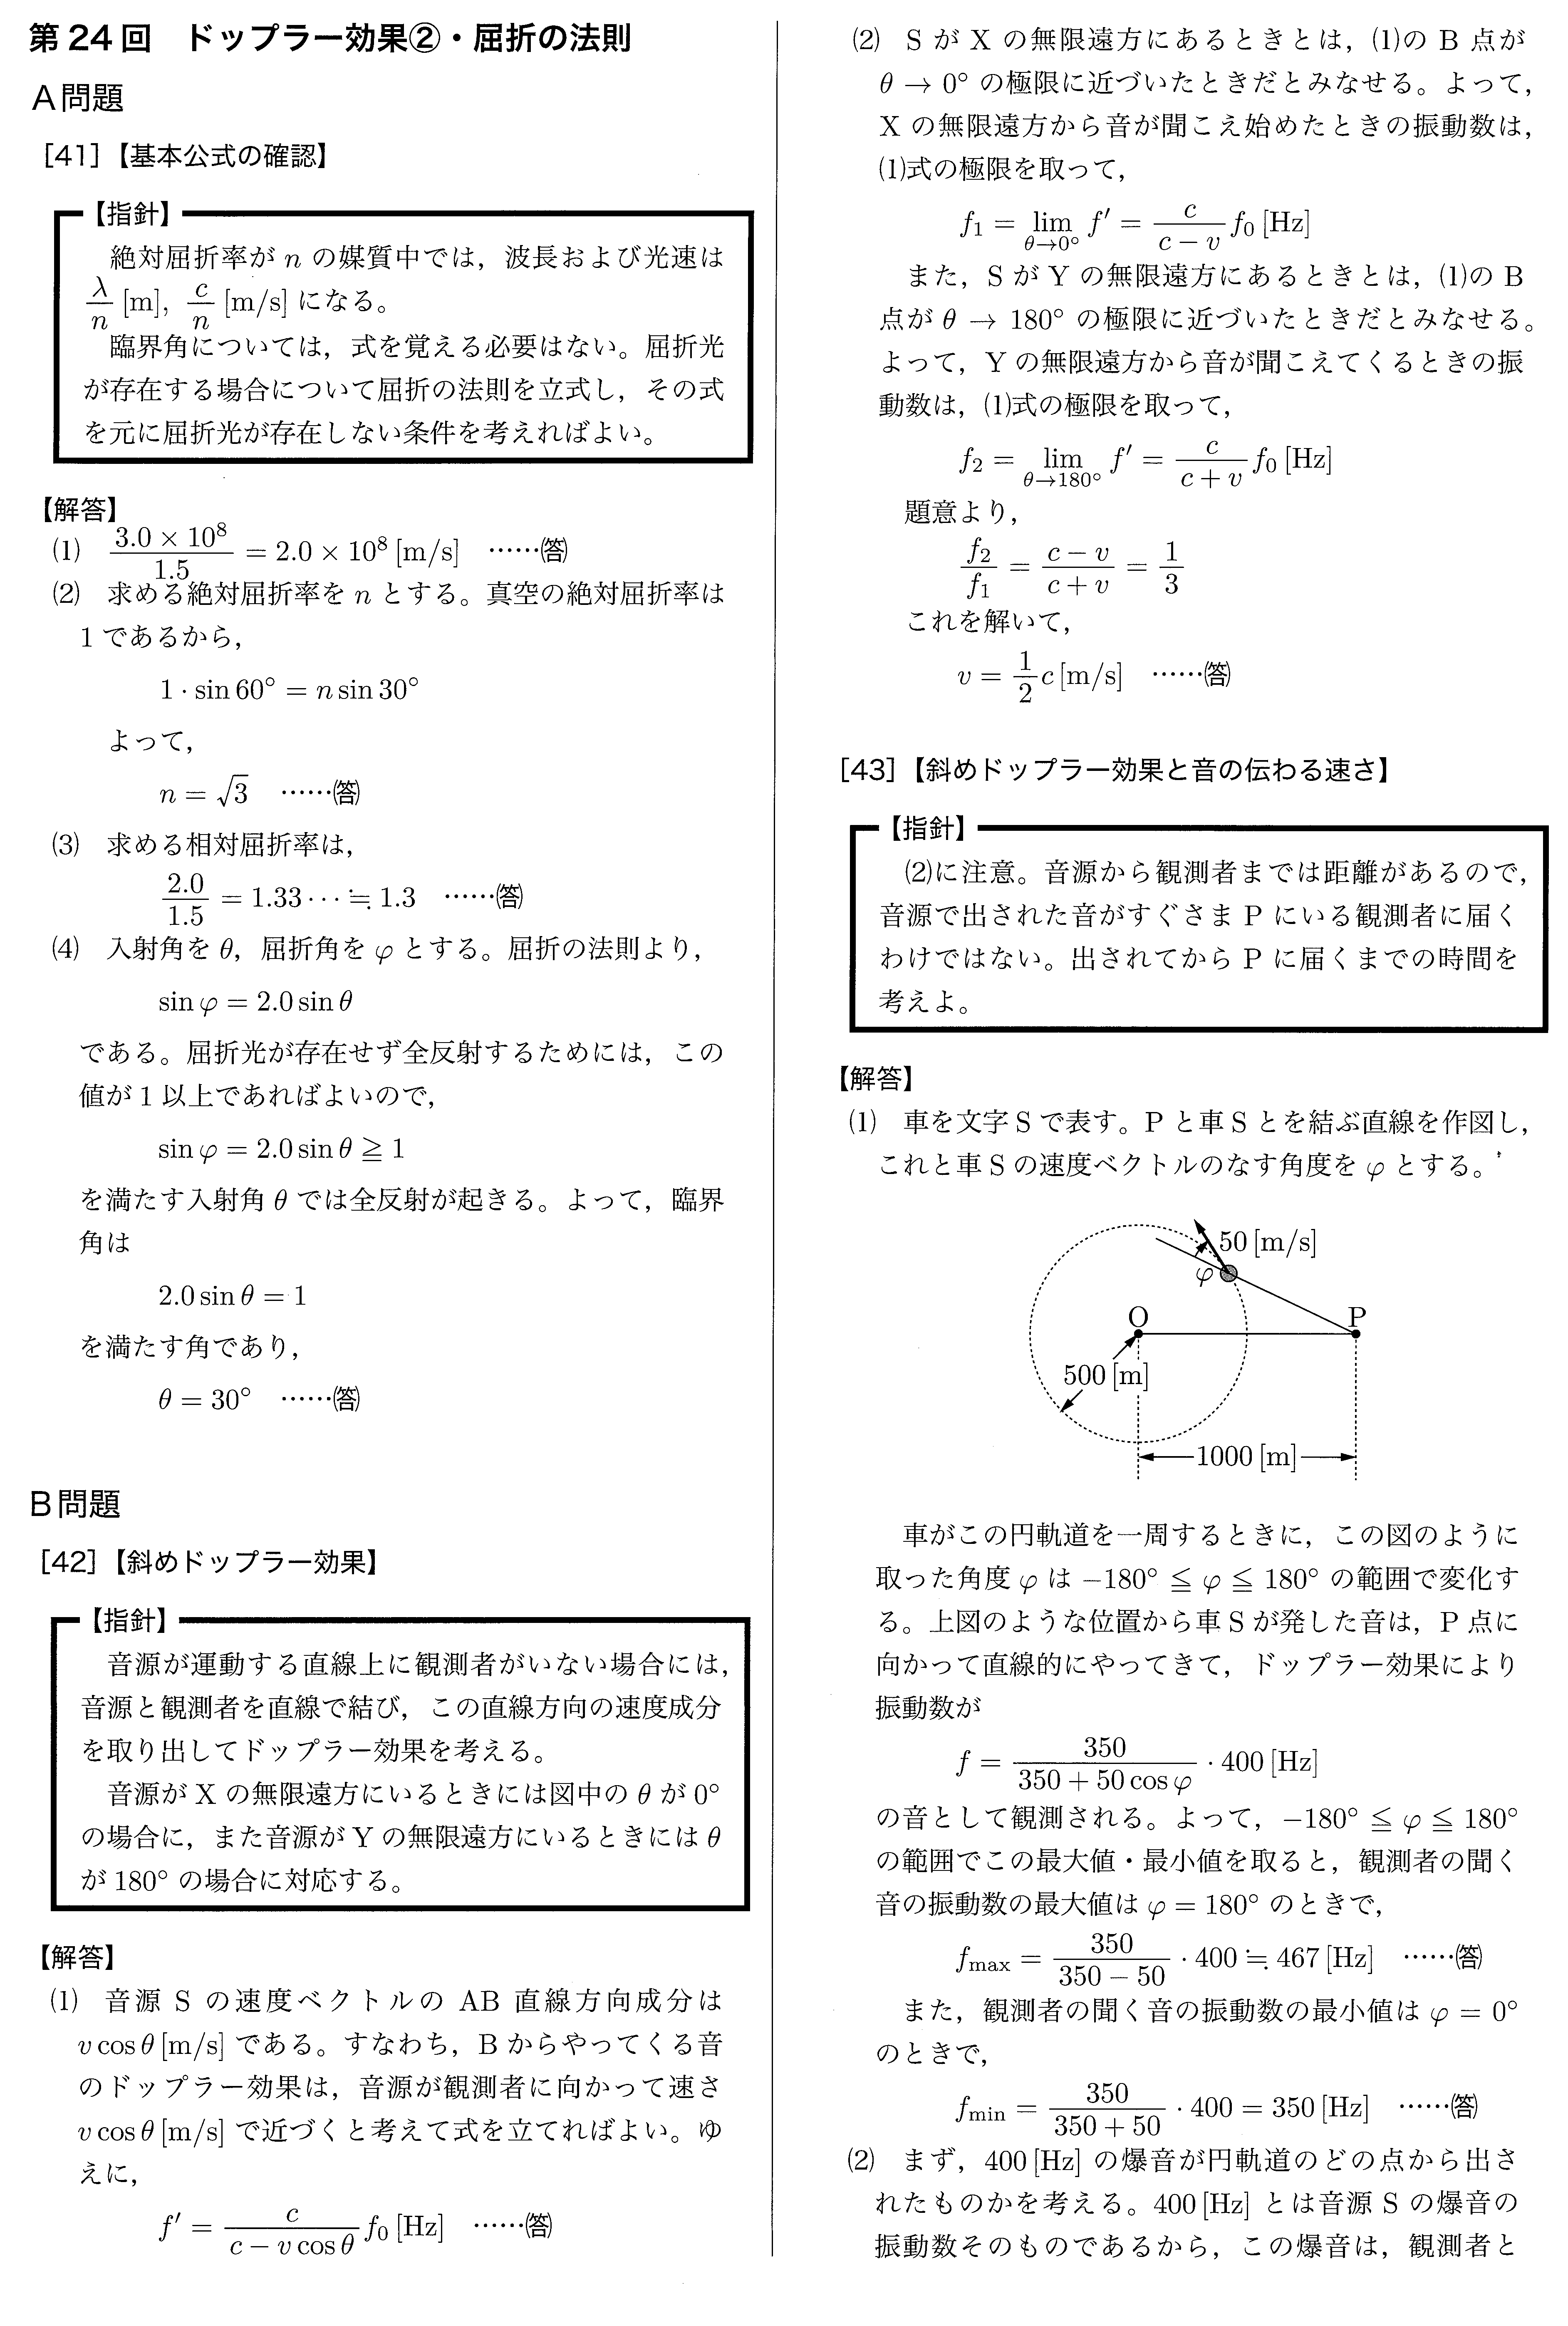
\includegraphics[width=170mm]{prob_p171.png}
\vspace{150mm}
\end{center}
\end{figure}

\newpage

\begin{figure}[h]
\begin{center}
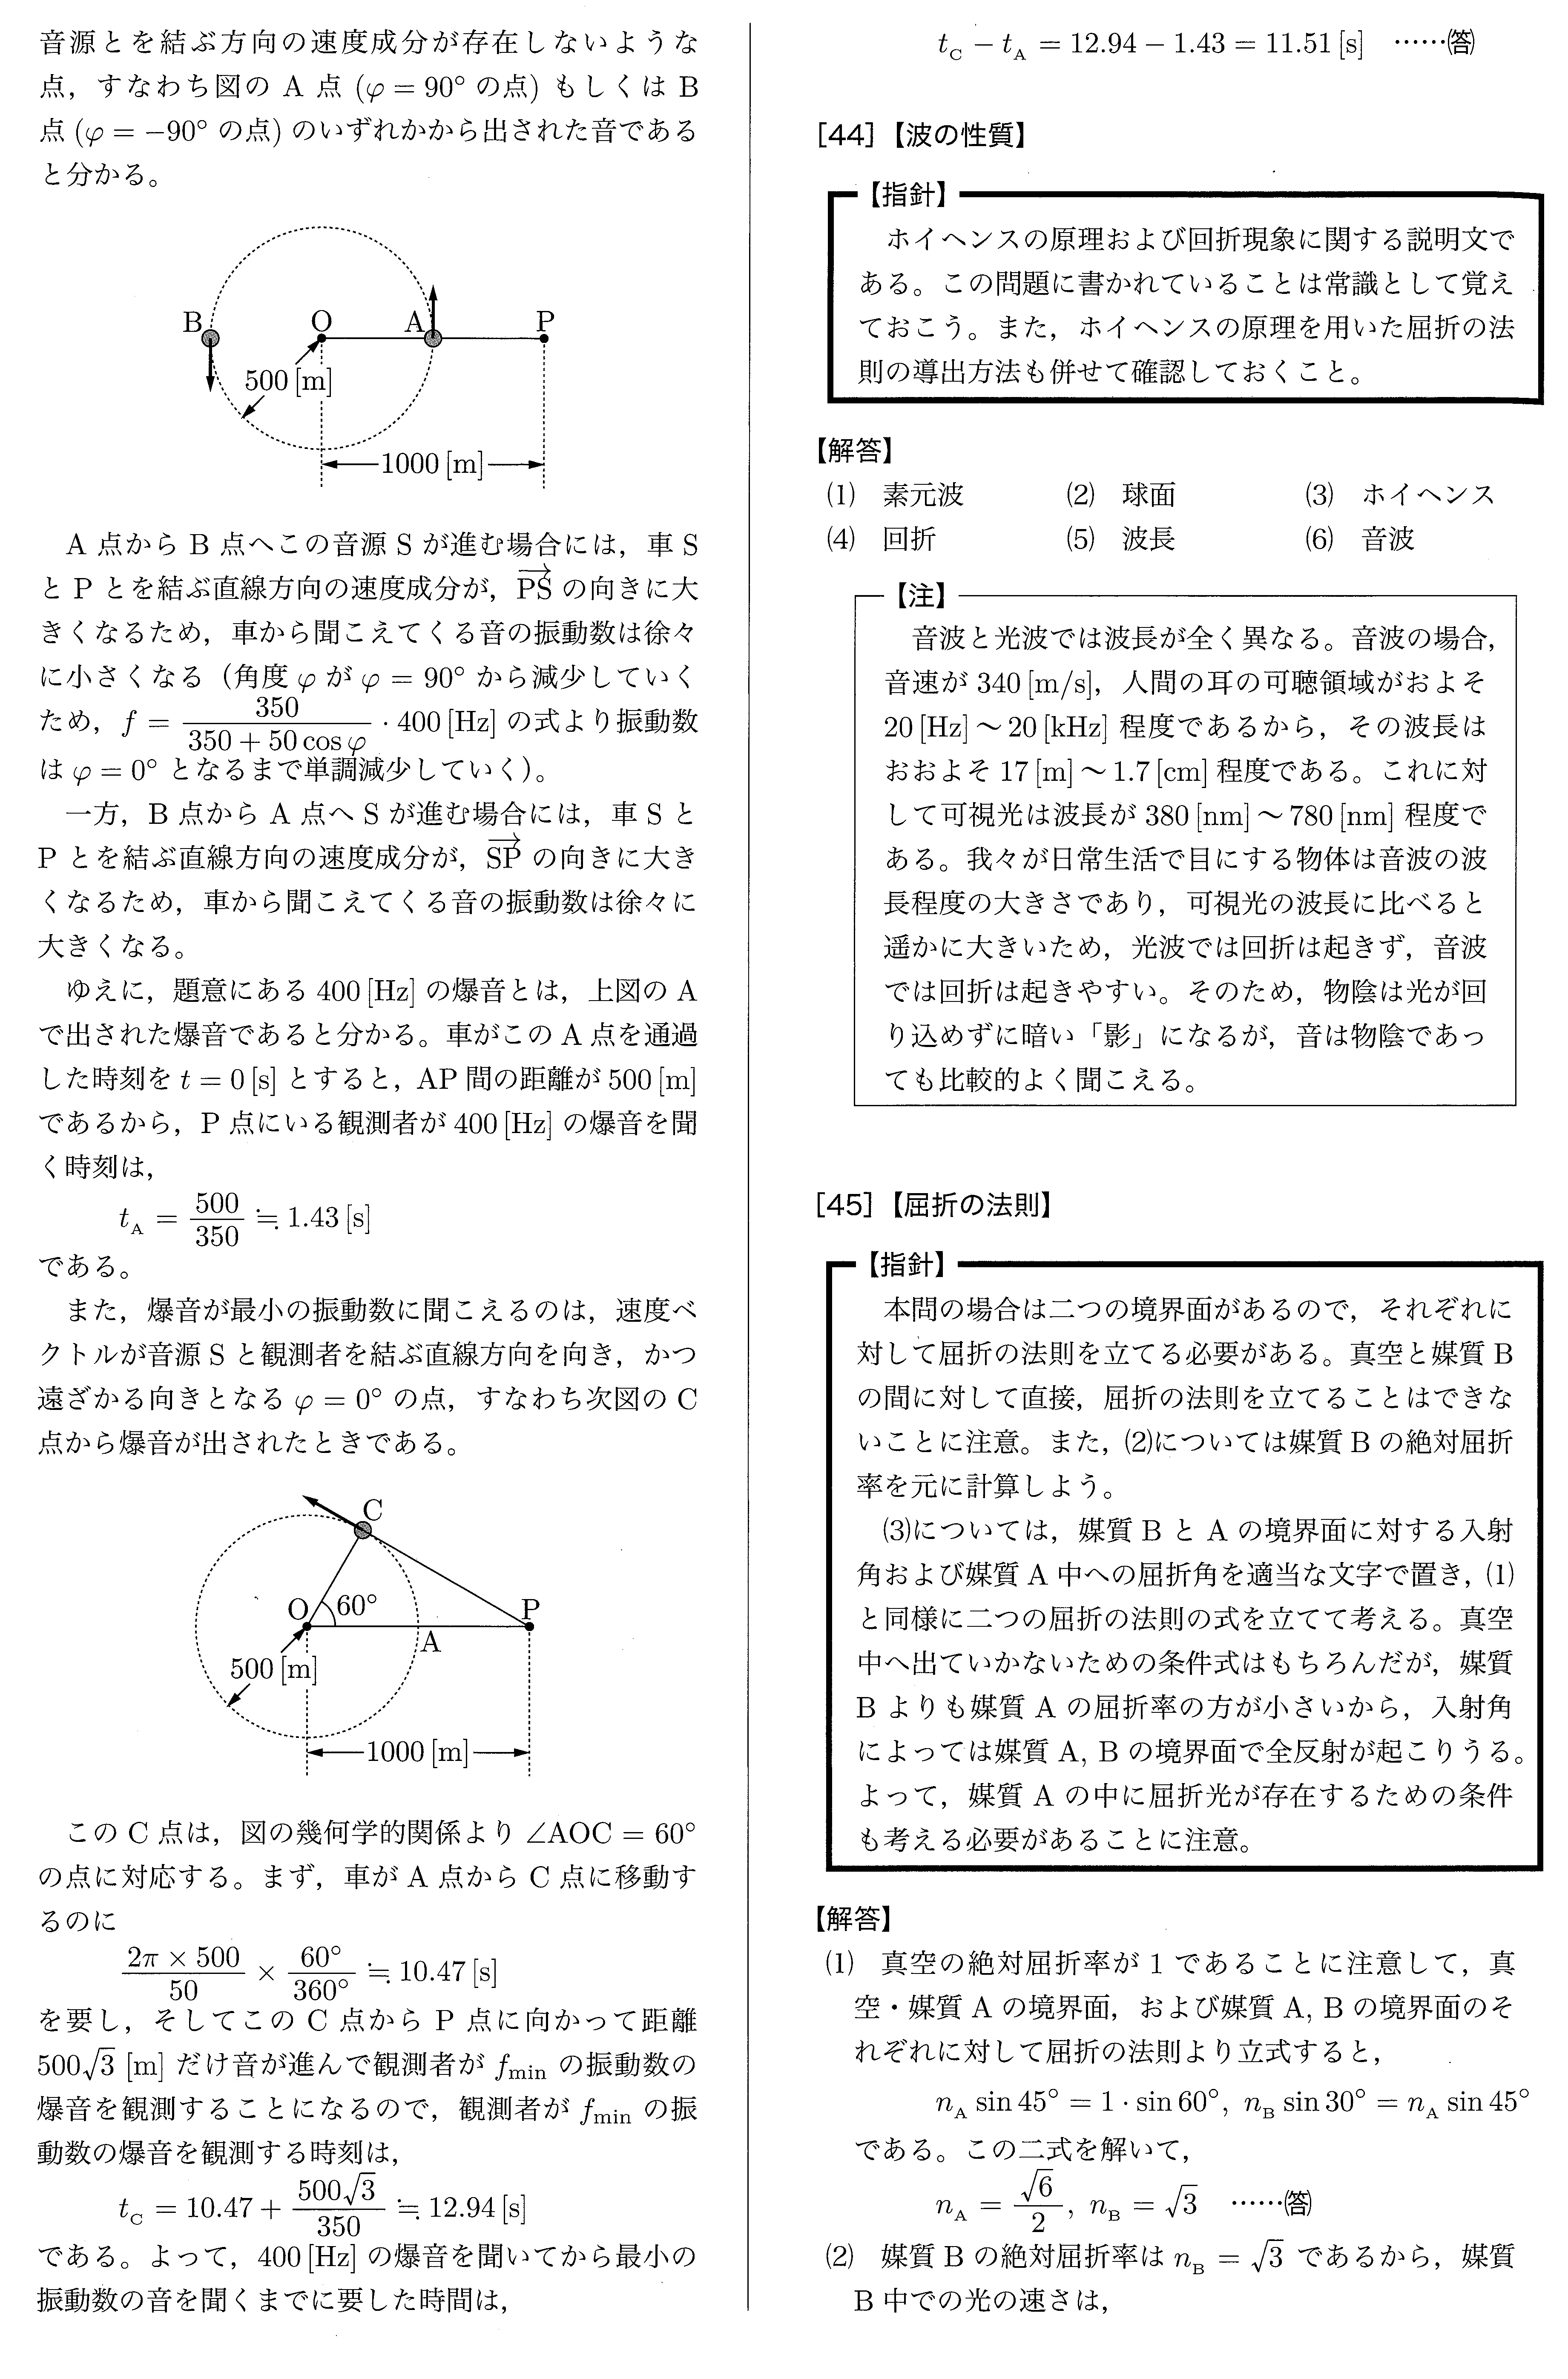
\includegraphics[width=170mm]{prob_p172.png}
\vspace{150mm}
\end{center}
\end{figure}

\newpage

\begin{figure}[h]
\begin{center}
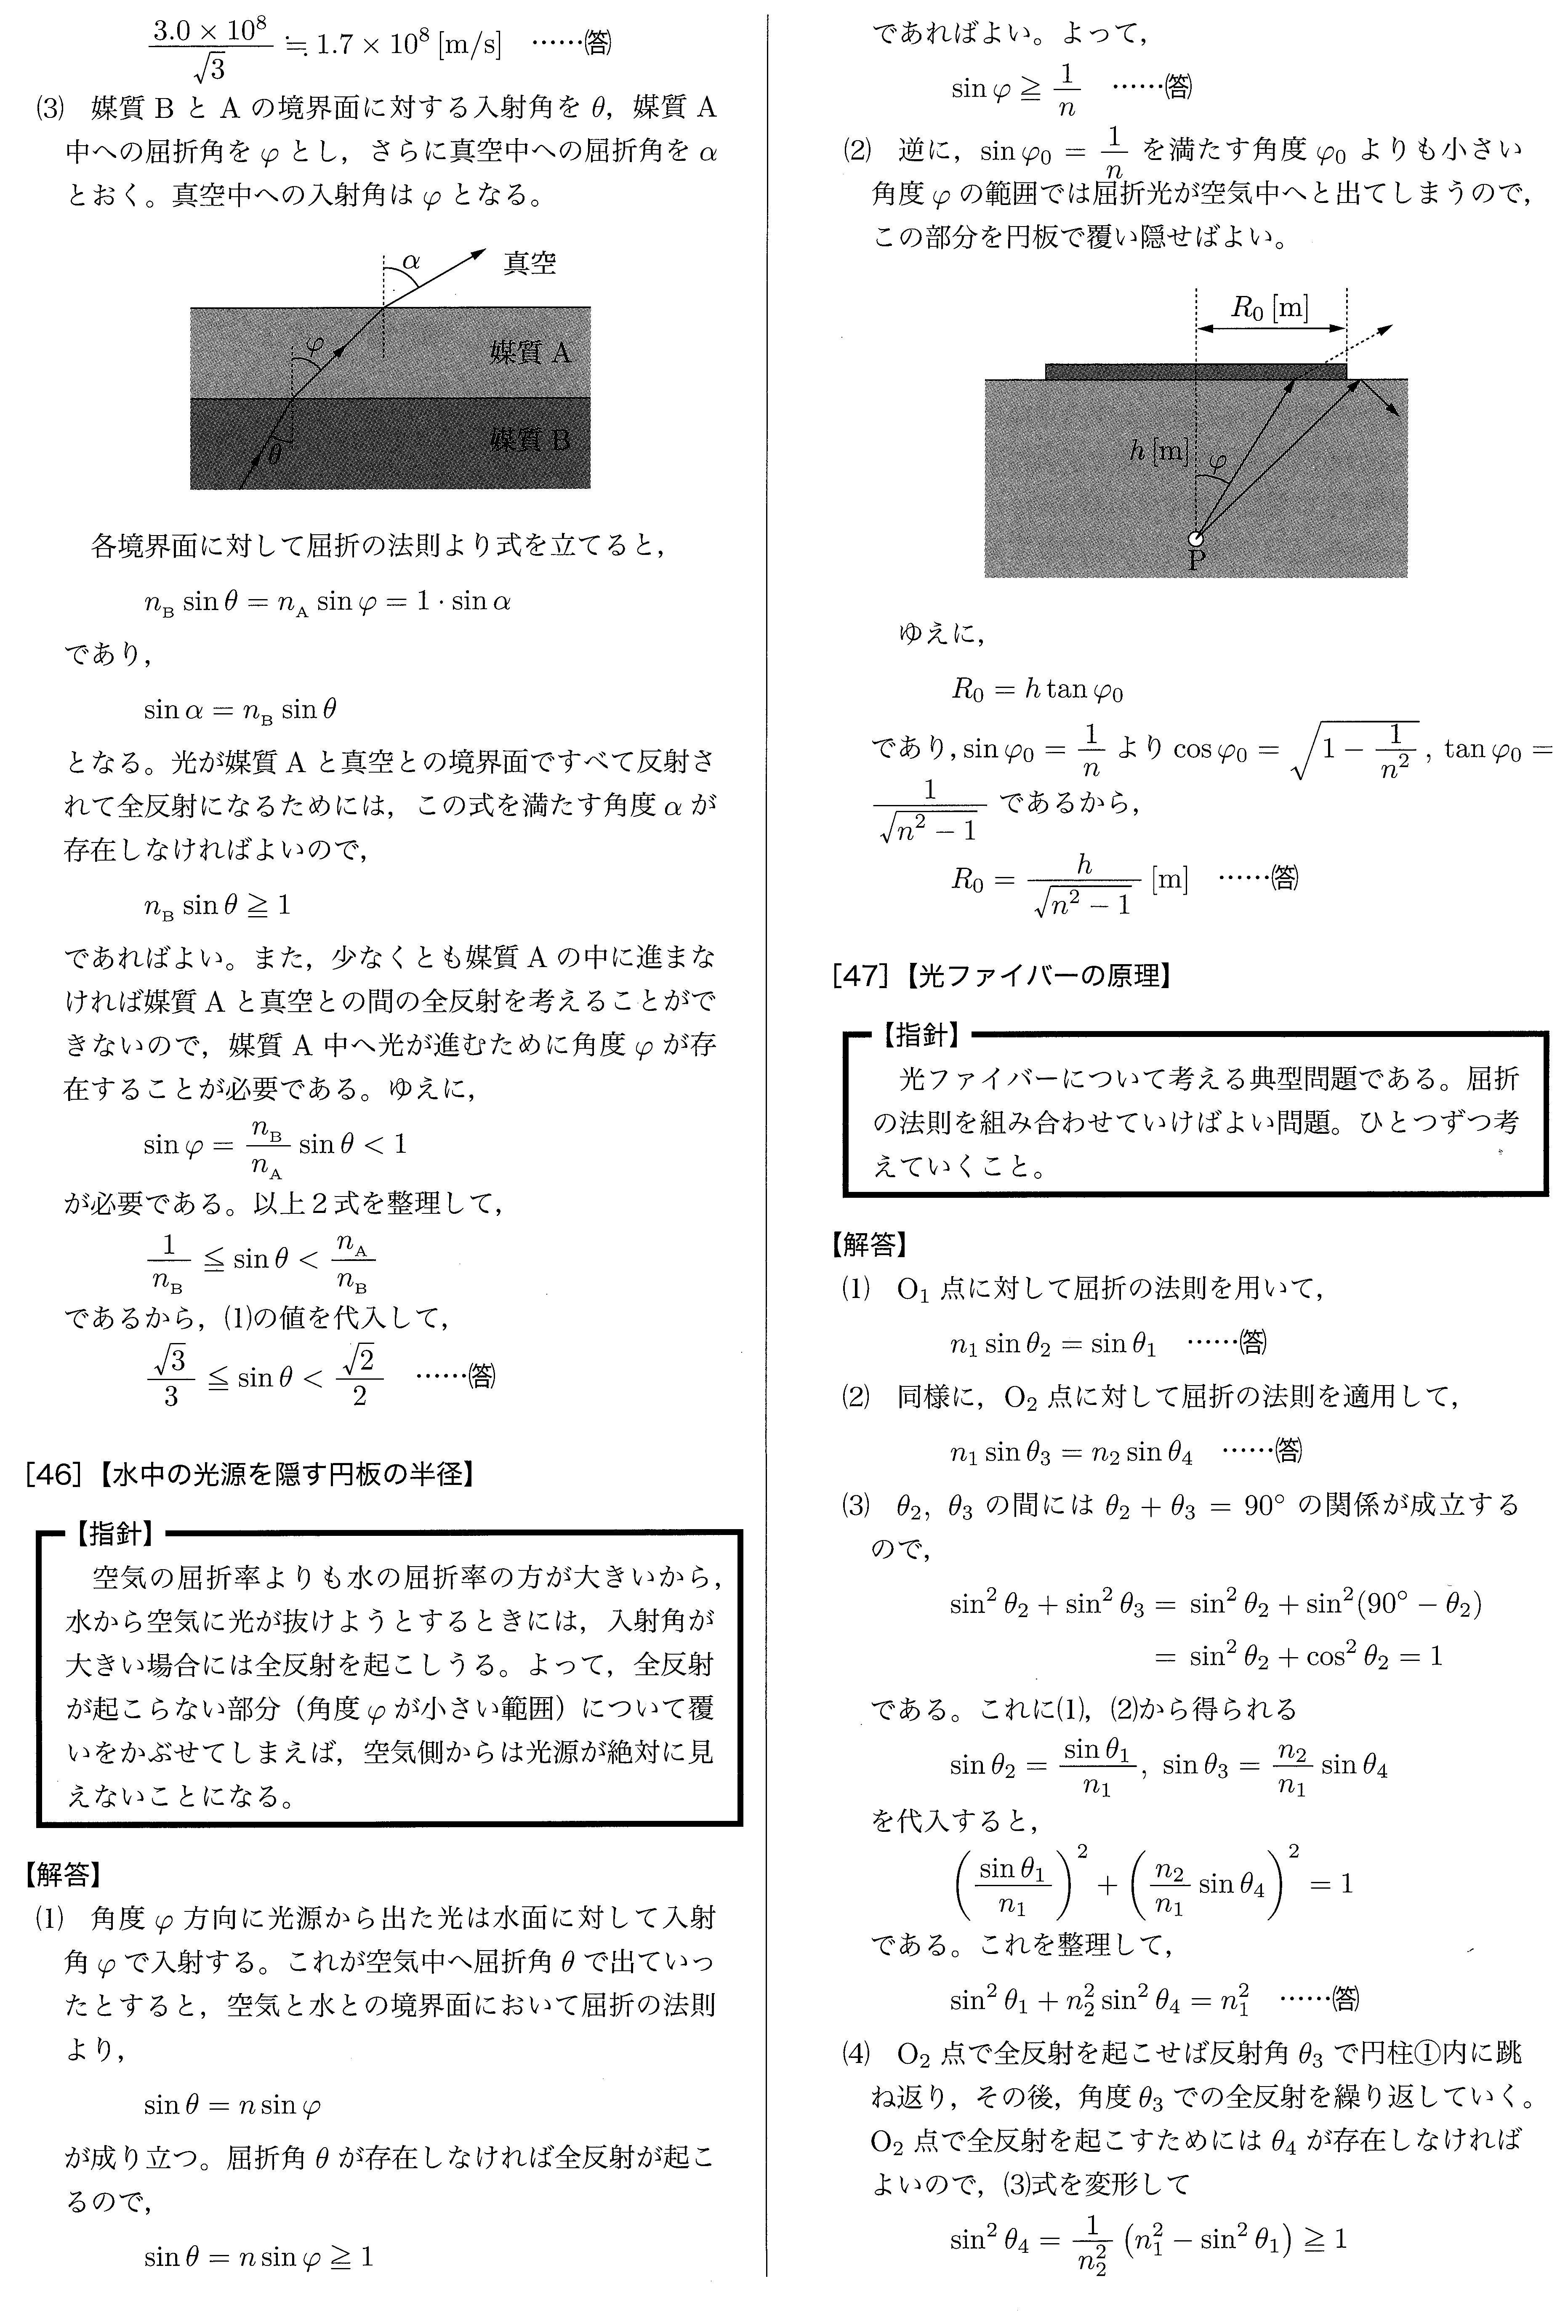
\includegraphics[width=170mm]{prob_p173.png}
\vspace{150mm}
\end{center}
\end{figure}

\newpage

\begin{figure}[h]
\begin{center}
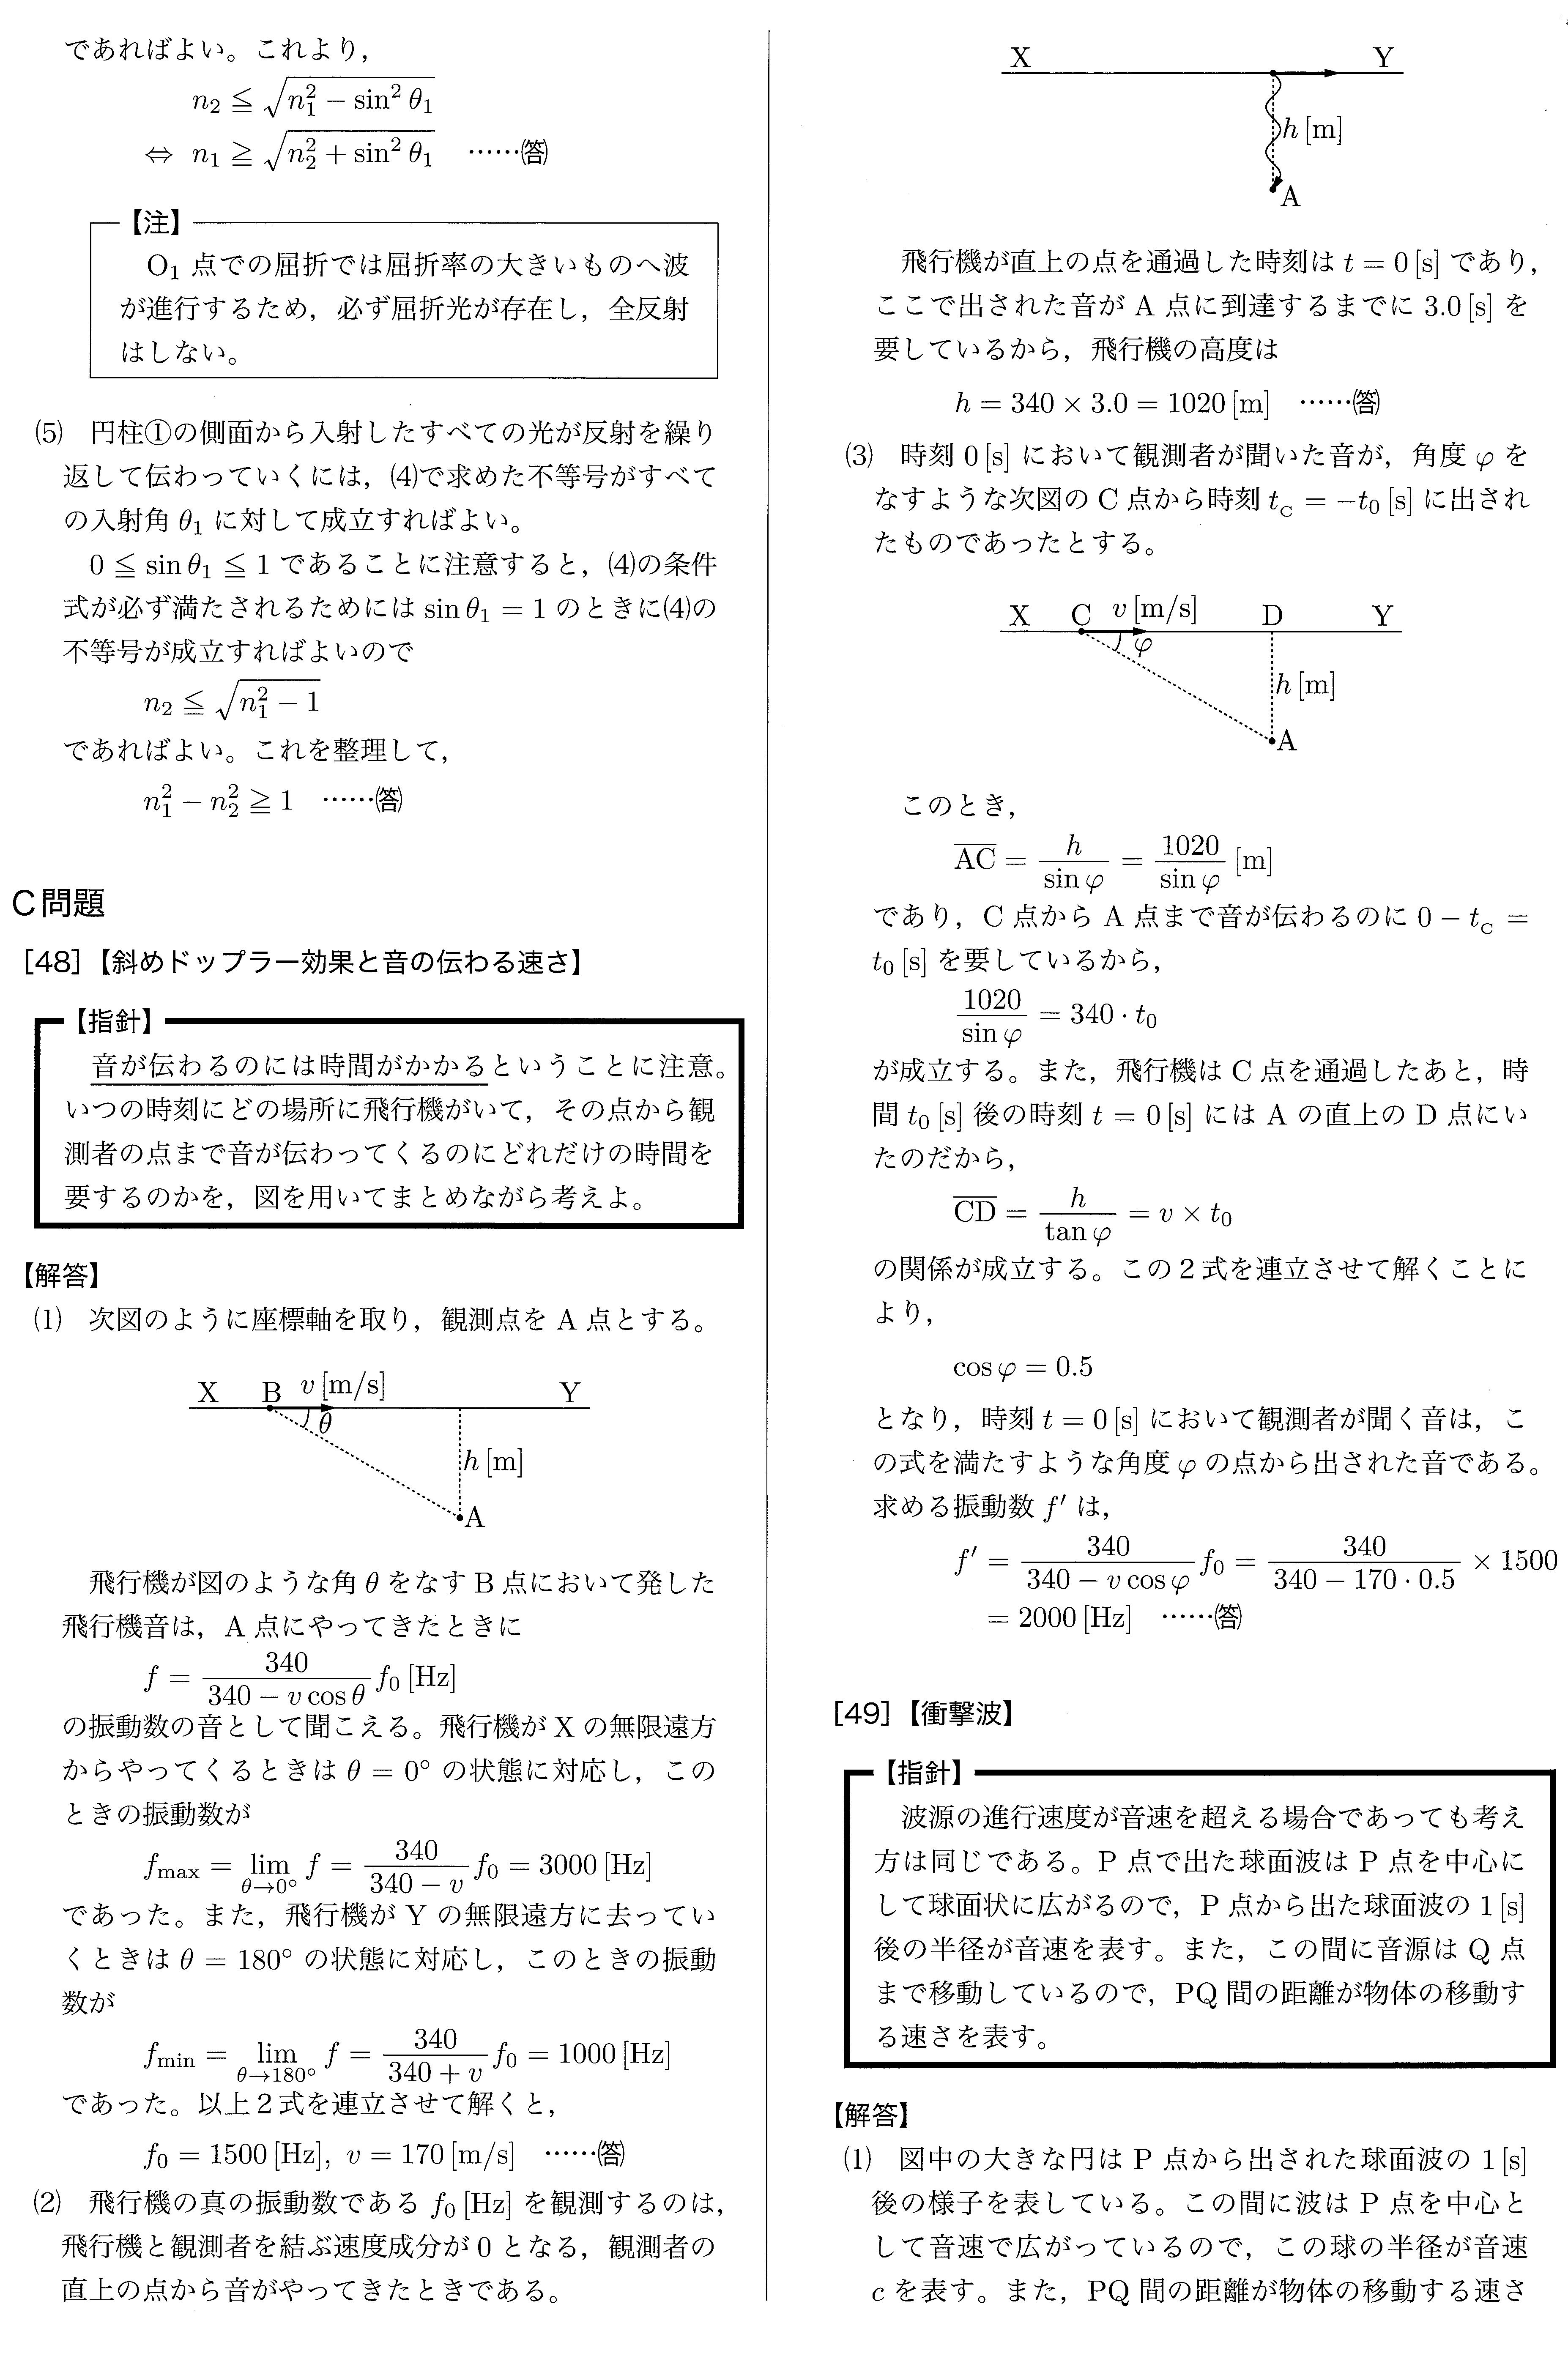
\includegraphics[width=170mm]{prob_p174.png}
\vspace{150mm}
\end{center}
\end{figure}

\newpage

\begin{figure}[h]
\begin{center}
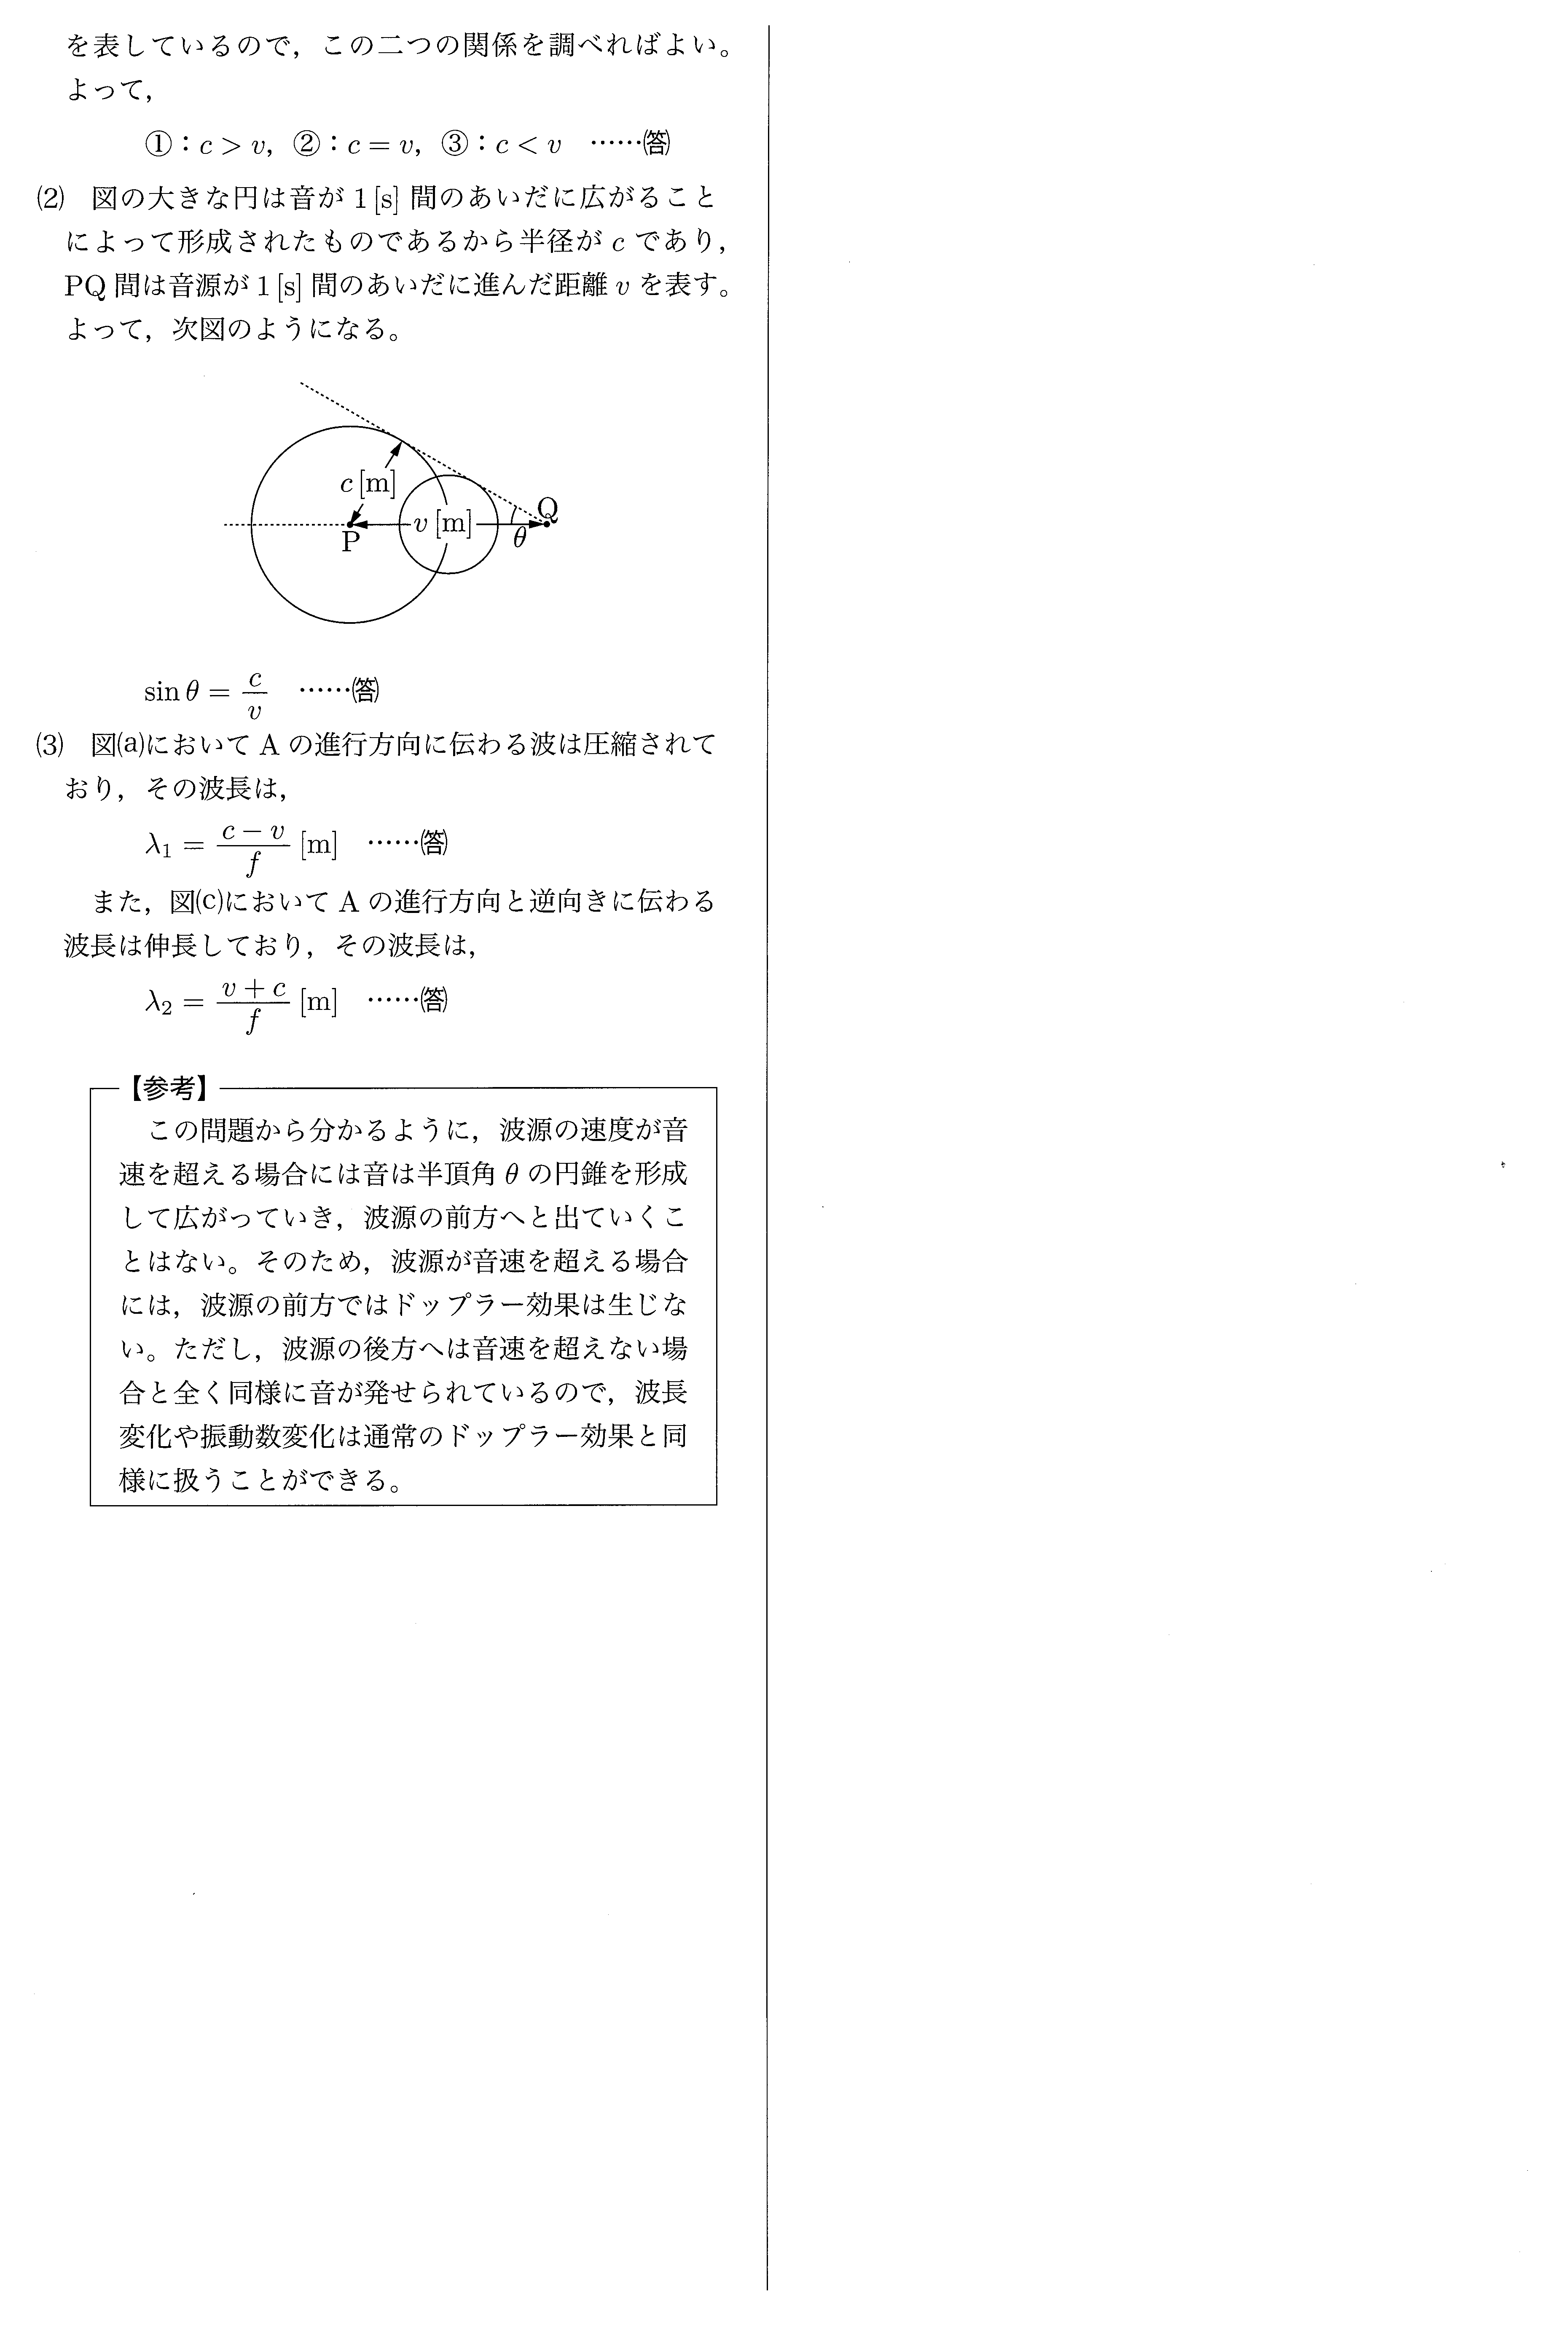
\includegraphics[width=170mm]{prob_p175.png}
\vspace{150mm}
\end{center}
\end{figure}


\include{physics_ch25}
 \ 
 
\newpage
\include{physics_ch26}
 \ 
 
\newpage
\section{レンズ(1)}

\subsection{凸レンズ}
\begin{wrapfigure}[13]{r}[5mm]{70mm}
  \centering
  \vspace{-5mm}
  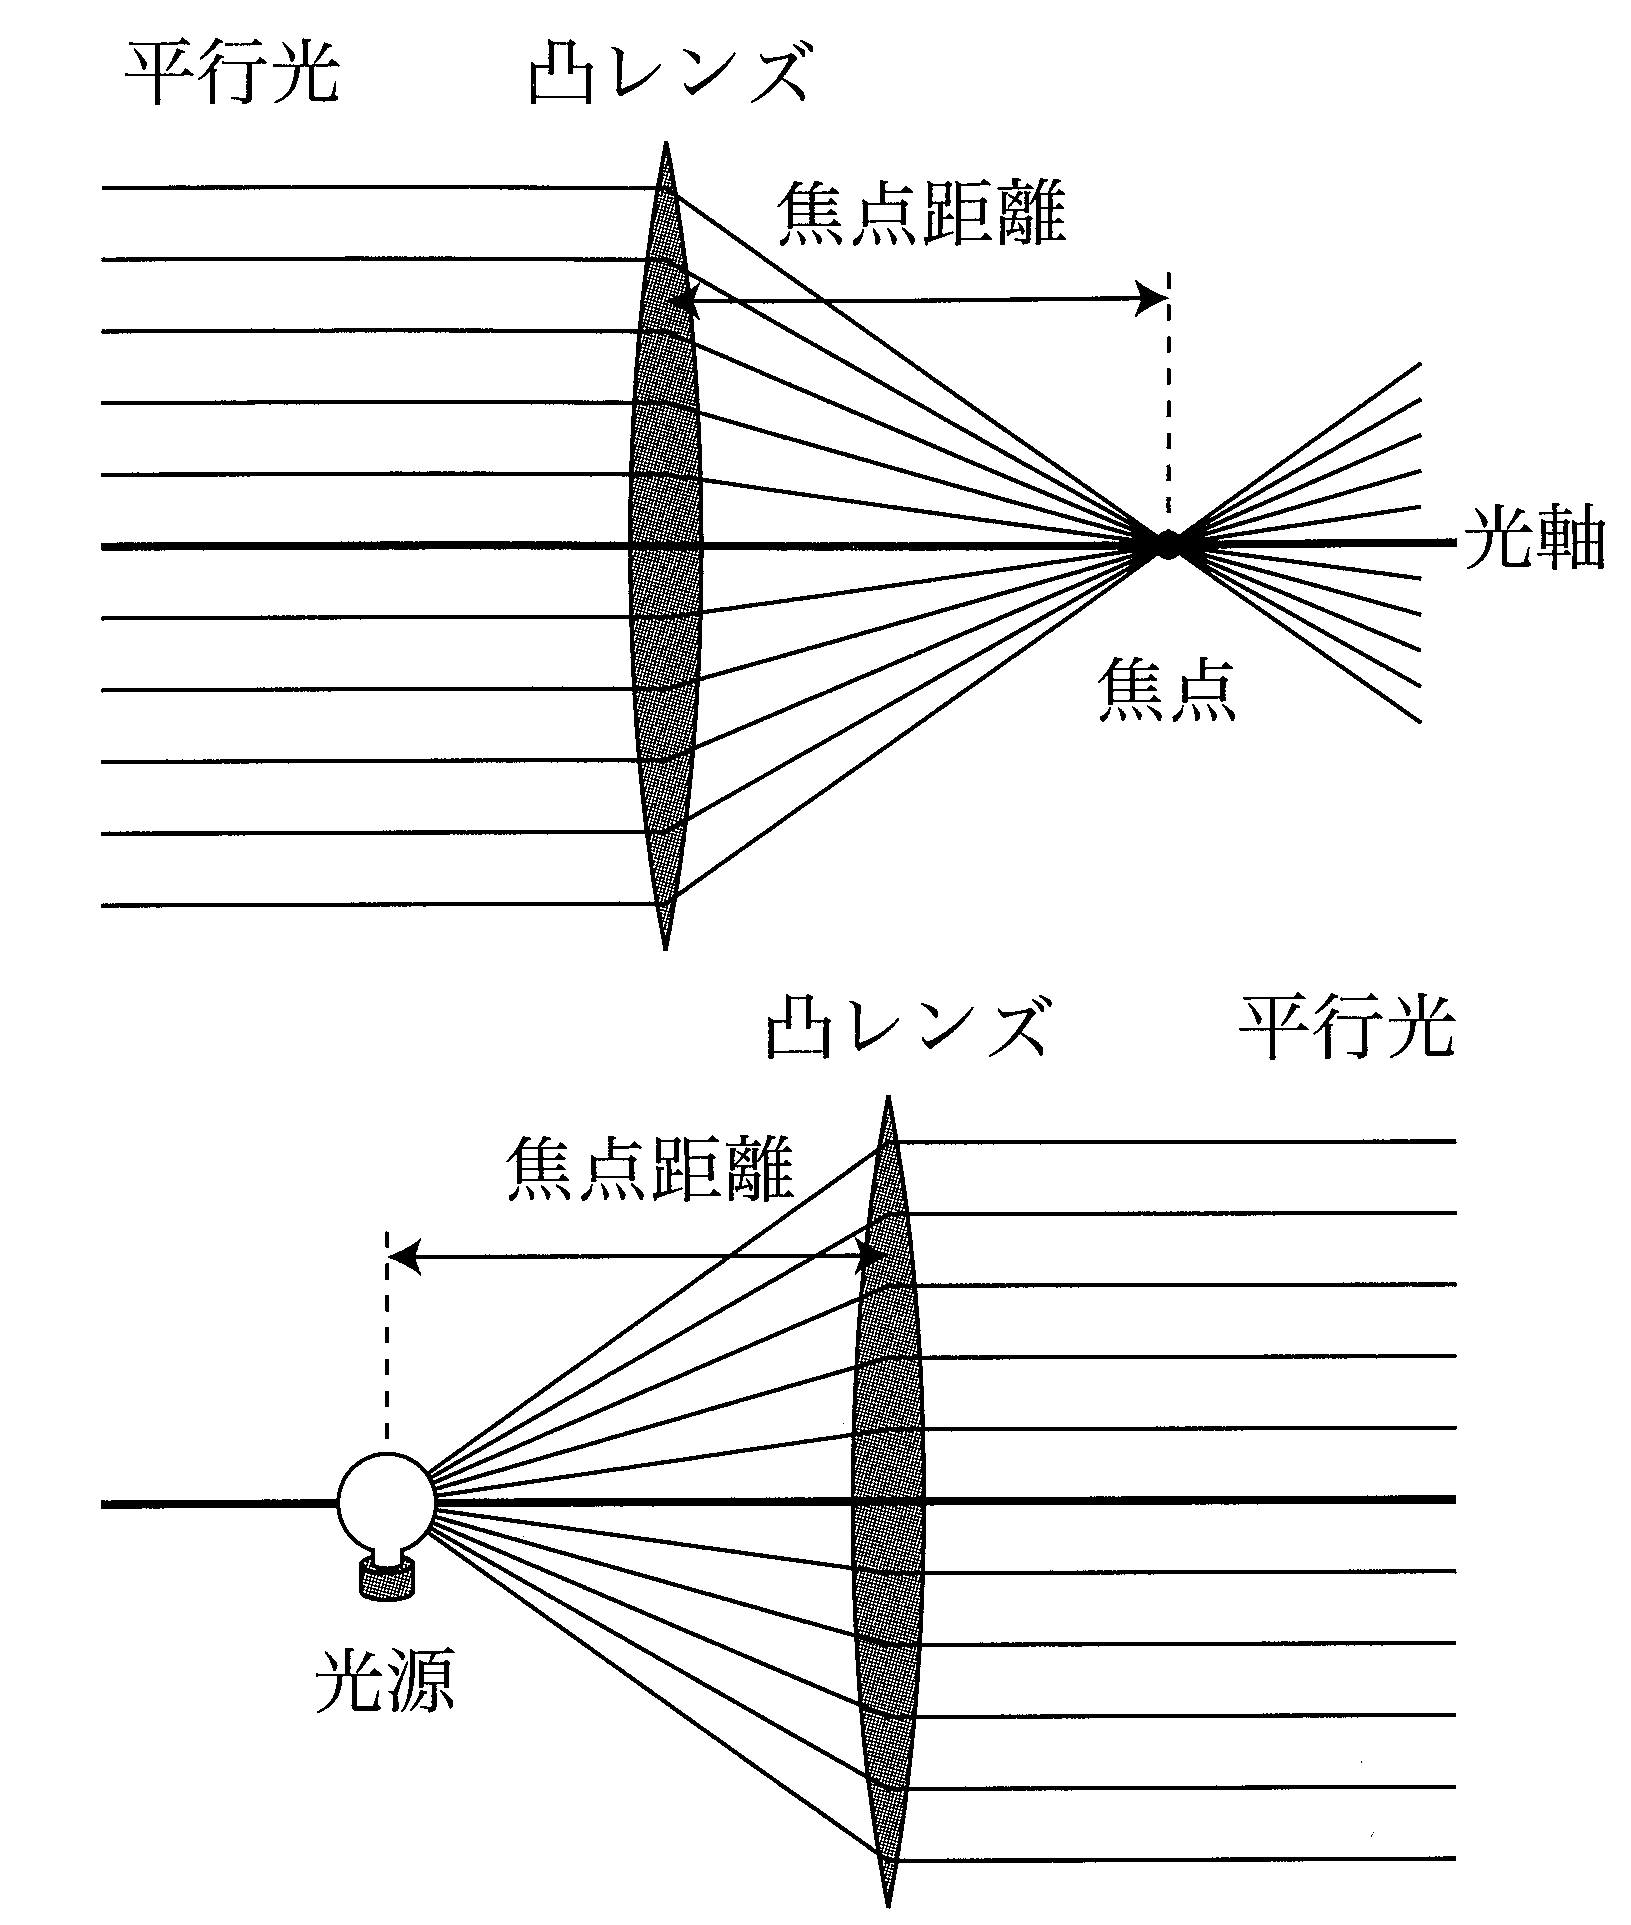
\includegraphics[keepaspectratio,width=70mm]
  {text2_p15_fig1.png}
\end{wrapfigure}
レンズは光の屈折を利用して光を集めたり発散させることができるもので，2つの球面によって挟まれたガラスなどでできている．
レンズには凸レンズと凹レンズがあるが，まず凸レンズについて考えてみよう．

レンズの2つの球面の中心を結ぶ直線をレンズの{\bf 光軸}という．
光軸に対して平行な光線を凸レンズにあてると，光はレンズの後方（向こう側）のある一点Fに集まる．
この点Fをレンズの{\bf 焦点}といい，レンズの中心から焦点までの距離をレンズの{\bf 焦点距離}という．
レンズの焦点はレンズの前方と後方に一つずつあり，いずれの焦点距離も等しい．
焦点に光源を置いた場合は先ほどのちょうど逆となり，レンズを通ると光軸に平行な光線群となる．\\[10mm]


次に，レンズより小さいサイズの物体を光軸上，手前の焦点よりも外側に置き，物体のある点Pから出ていく以下の3つの光について考える．\vspace{5mm}

\begin{wrapfigure}[8]{r}[5mm]{90mm}
  \centering
  \vspace{-5mm}
  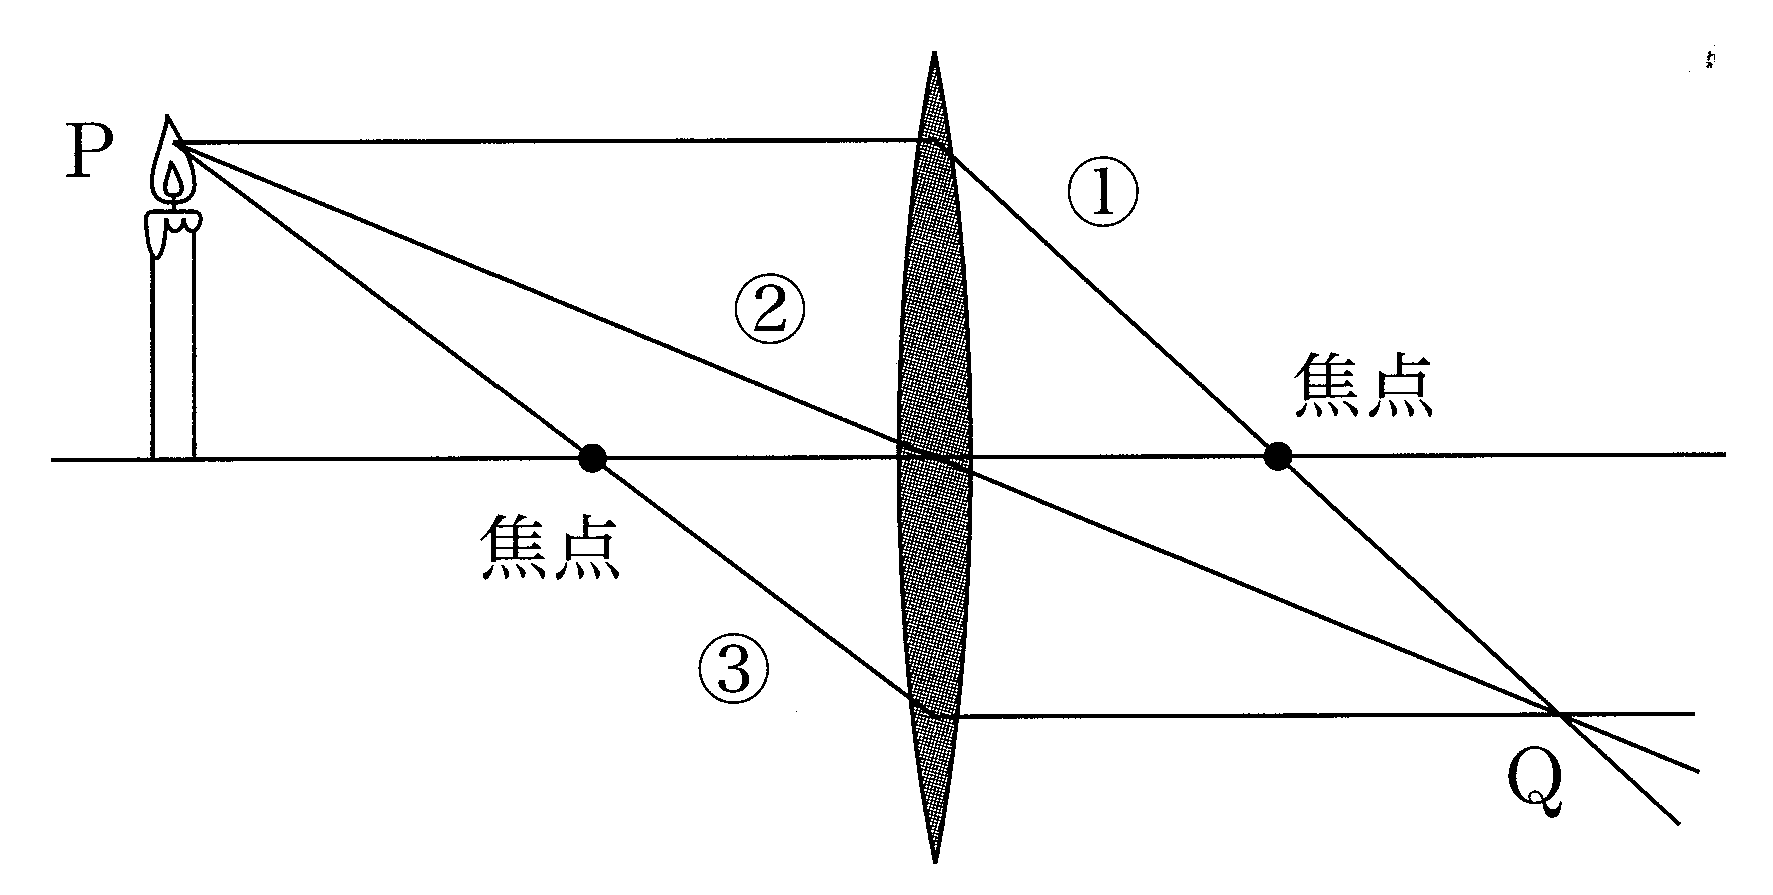
\includegraphics[keepaspectratio,width=90mm]
  {text2_p15_fig2.png}
\end{wrapfigure}
$\MARU{1}$\hspace{2mm} {\bf 光軸に平行に出た光}

この光はレンズの向こう側の焦点を通るように進む．

$\MARU{2}$\hspace{2mm} {\bf レンズの中心を通過する光}

この光は曲がらずに直進する．（レンズの厚さが無視できるとき）

$\MARU{3}$\hspace{2mm} {\bf 手前側の焦点を通る光}

この光はレンズの向こう側に出ると光軸に平行な光線となる．\vspace{5mm}

今は3つのみについて考えたが，点Pから出てレンズに入った光は$\MARU{1},\MARU{2},\MARU{3}$に限らず，{\bf すべて同一の点Qを通る．}
そのため，光軸に対して垂直でQ点を含む面に紙を置くと，紙面には光源の像が生じる．
この像のように，実際に光が集まって作られる像を{\bf 実像}と呼ぶ．
この場合，像は光源の物体に対して逆さまになっているので，これを{\bf 倒立像}と呼ぶ．
これに対し像が同じ向きになっているものは{\bf 正立像}と呼ぶ．

なお，実際の像の位置の把握には，上述の3つのうち2つを考えれば十分である．

\newpage
\subsection{凹レンズ}
\begin{wrapfigure}[15]{r}[5mm]{70mm}
  \centering
  \vspace{-5mm}
  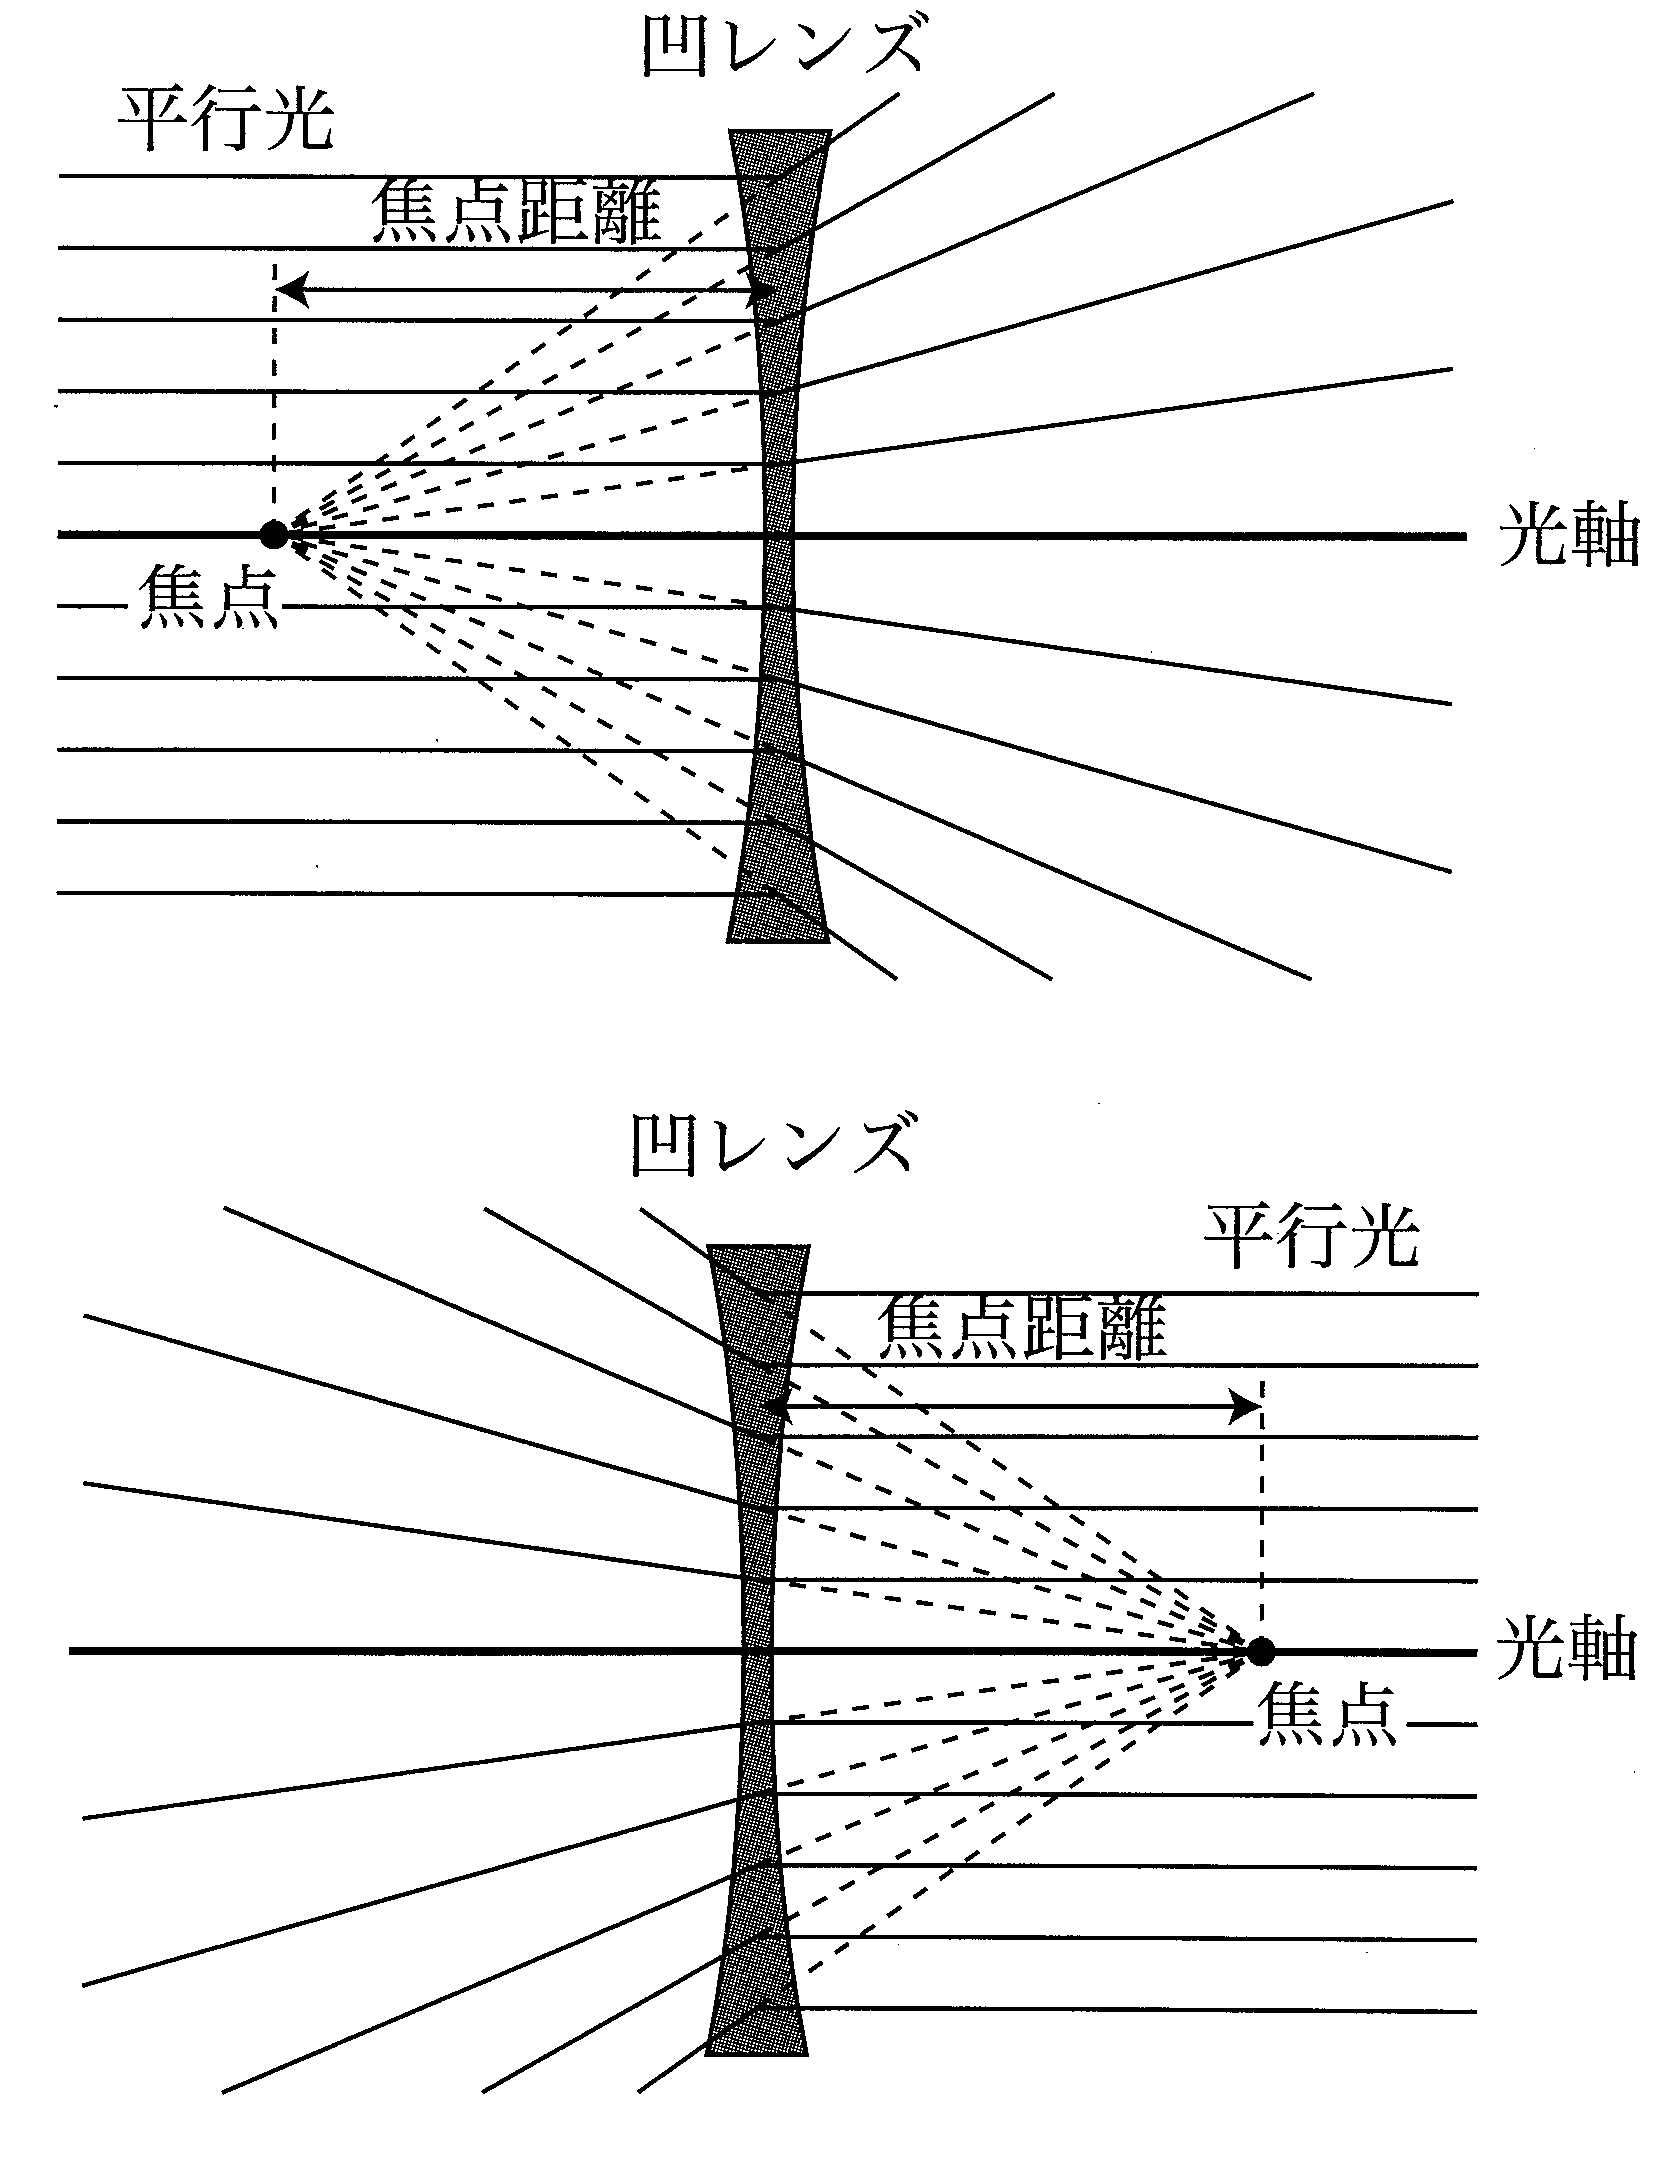
\includegraphics[keepaspectratio,width=70mm]
  {text2_p16_fig1.png}
\end{wrapfigure}
凹レンズは周辺部よりも中心部が凹んでいる形のレンズである．
凹レンズの光軸に対して平行な光線をあてると，光はレンズを通ると図のように広がっていく．
この広がっていく光線をレンズの手前側まで伸ばすと，直線はある一点で交わる．
すなわち，レンズにより発散した光線はこの一点から直進して出ていった光と同様になる．
この点を凹レンズの{\bf 焦点}という．

凹レンズについても凸レンズ同様，レンズの前方と後方に焦点が一つずつあり，その焦点距離はいずれも等しい．
またレンズの向こう側にある焦点に光を集めるように凹レンズに光を入射すると，その光は凹レンズを通過した後，光軸に平行な光線群となる．\\[10mm]

次にレンズより小さいサイズの物体を光軸上，焦点よりも外側に置き，物体のある点Pから出ていく以下の3つの光について考える．\vspace{5mm}

\begin{wrapfigure}[8]{r}[5mm]{90mm}
  \centering
  \vspace{-5mm}
  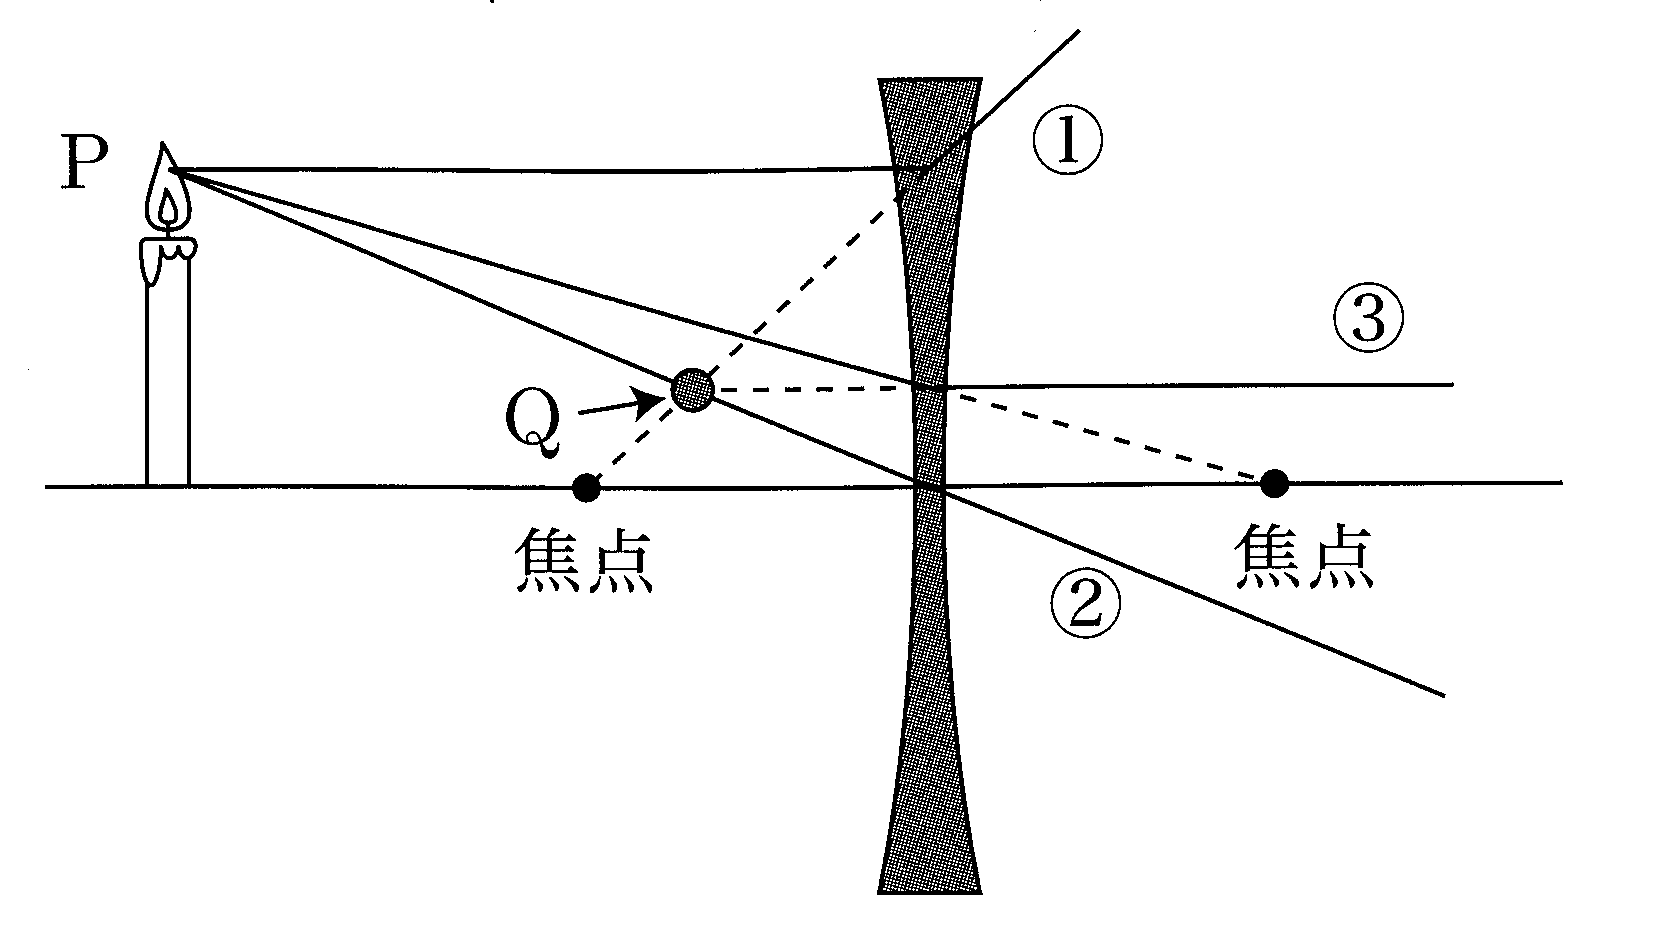
\includegraphics[keepaspectratio,width=90mm]
  {text2_p17_fig1.png}
\end{wrapfigure}
$\MARU{1}$\hspace{2mm} {\bf 光軸に平行に出た光}

この光はレンズの手前側の焦点から直進するように進む．

$\MARU{2}$\hspace{2mm} {\bf レンズの中心を通過する光}

この光は曲がらずに直進する．（レンズの厚さが無視できるとき）

$\MARU{3}$\hspace{2mm} {\bf 向こう側の焦点へ直進する光}

この光はレンズの向こう側に出ると光軸に平行な光線となる．\vspace{5mm}

レンズの向こう側に出た$\MARU{1} 〜\MARU{3}$の3つの光線はレンズの向こう側では交わらないが，これらの光線をレンズの手前側に戻してやると，それらは図のQ点の一点に交わる．
すなわち，レンズの向こう側の光線は，Qの位置から直進して出てきた光のように広がっていく．
そのため，レンズの向こう側からレンズを覗き見るとあたかもQに物体があるかのように見える．
このQを{\bf 虚像}という．
虚像は実像と異なり，実際にその位置に光が集まってはいないため虚像の位置に紙を置いても像は写らない．

\newpage
\subsection{虚光源}
\begin{wrapfigure}[10]{r}[5mm]{70mm}
  \centering
  \vspace{-5mm}
  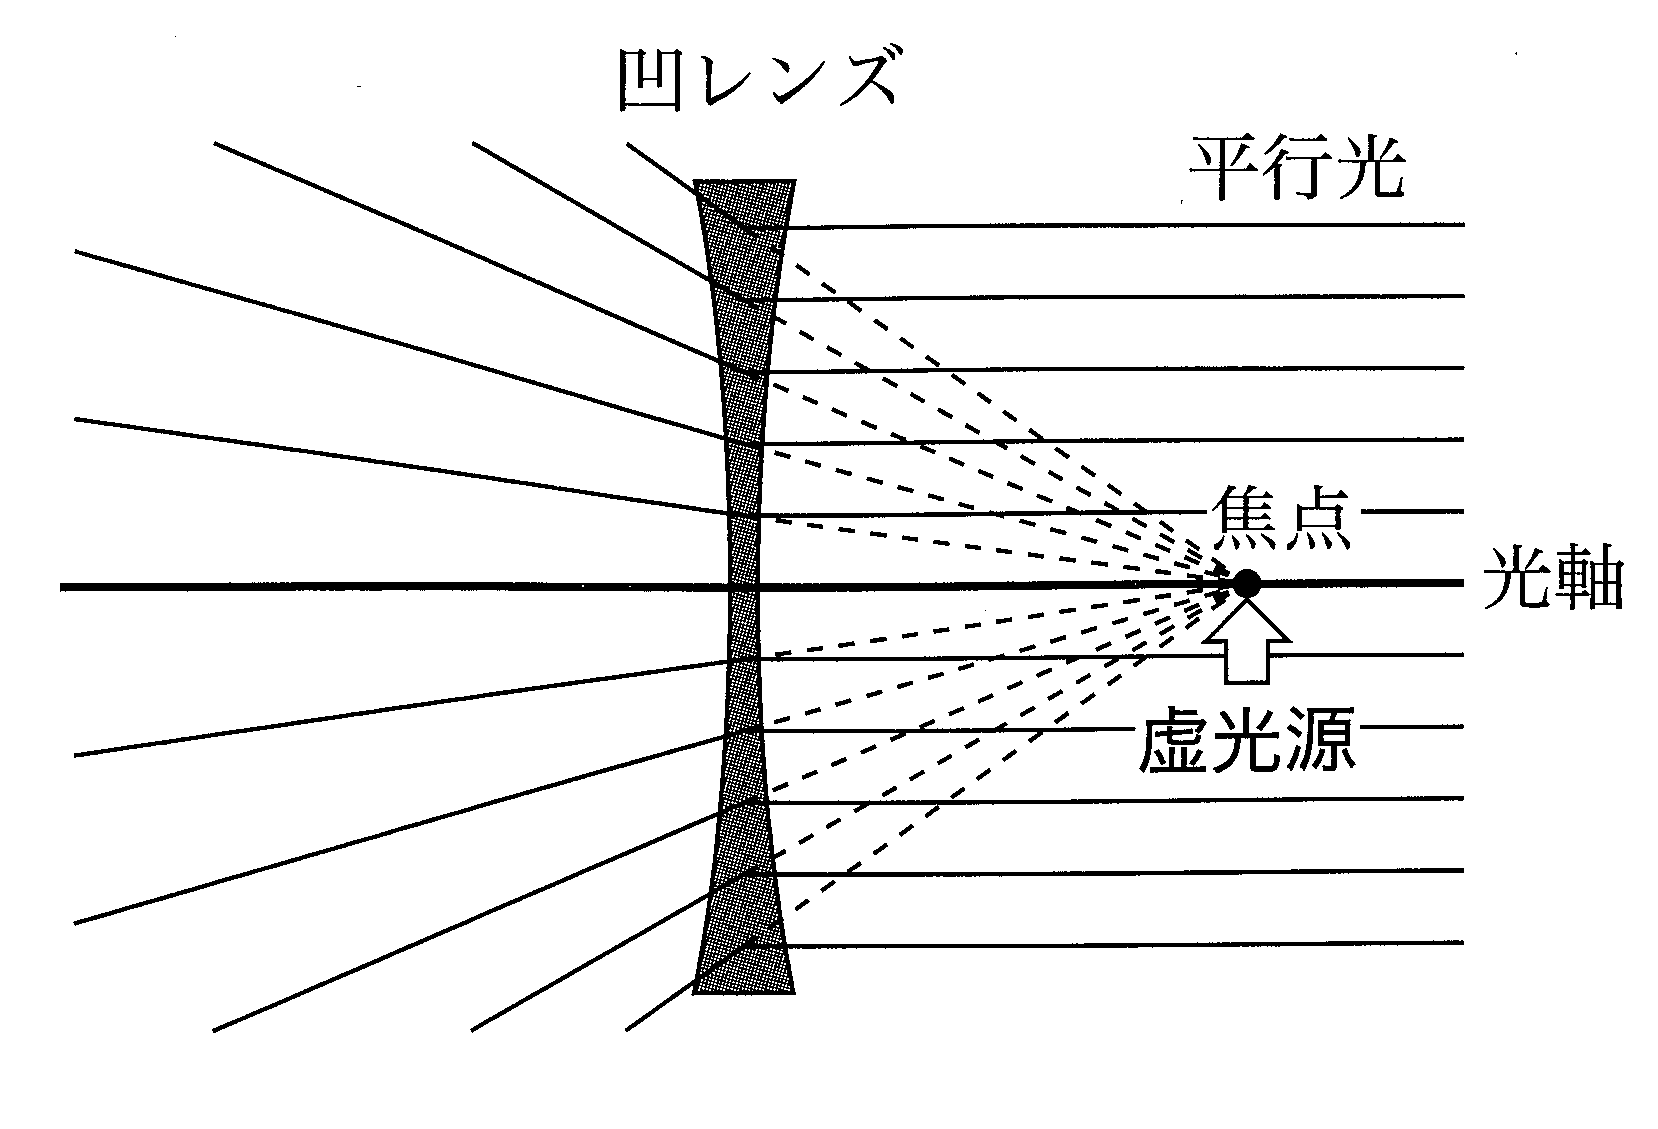
\includegraphics[keepaspectratio,width=70mm]
  {text2_p19_fig1.png}
\end{wrapfigure}
凹レンズに対し，レンズの向こう側にある焦点に光を集めるように凹レンズの光を入射すると，その光は凹レンズを通過した後，光軸に平行な光線群となる．

ここで考えた，レンズの向こう側にある焦点に向かう光は，凹レンズよりも手前に凸レンズを置くことにより作ることができる．

このように，レンズの向こう側にある一点に向かう光線群において，集光しようとしている場所を{\bf 虚光源}と呼ぶ．

光源，像の位置を次のように定義し直すと，虚光源や虚像もまとめて定義することができる．

   \begin{matome}{光源と像}
   
\hspace{2mm}$\MARU{1}$\hspace{2mm} {\bf 光源}\\
 \hspace{3mm} {\bf レンズに入射する直前の光線群（またはその延長）が一点に集まる場所．}
 光の進行方向に対して，その場所がレンズより手前ならば{\bf 実光源}，レンズより奥ならば{\bf 虚光源}となる．
 実際に光線群が光源の位置で集光しているかどうかは光源の位置を決定する上で関係がない．

\hspace{2mm}$\MARU{2}$\hspace{2mm} {\bf 像}\\
 \hspace{3mm} {\bf レンズにより屈折された直後の光線群（またはその延長）が一点に集まる場所．}
光の進行方向に対して，その場所がレンズよりも奥ならば{\bf 実像}，レンズより手前ならば{\bf 虚像}となる．
 実際に光線群が像の位置で集光しているかどうかは像の位置を決定する上で関係がない．\\[27mm]
 \end{matome}
 \begin{figure}[h]
\begin{center}
\vspace{-40mm}
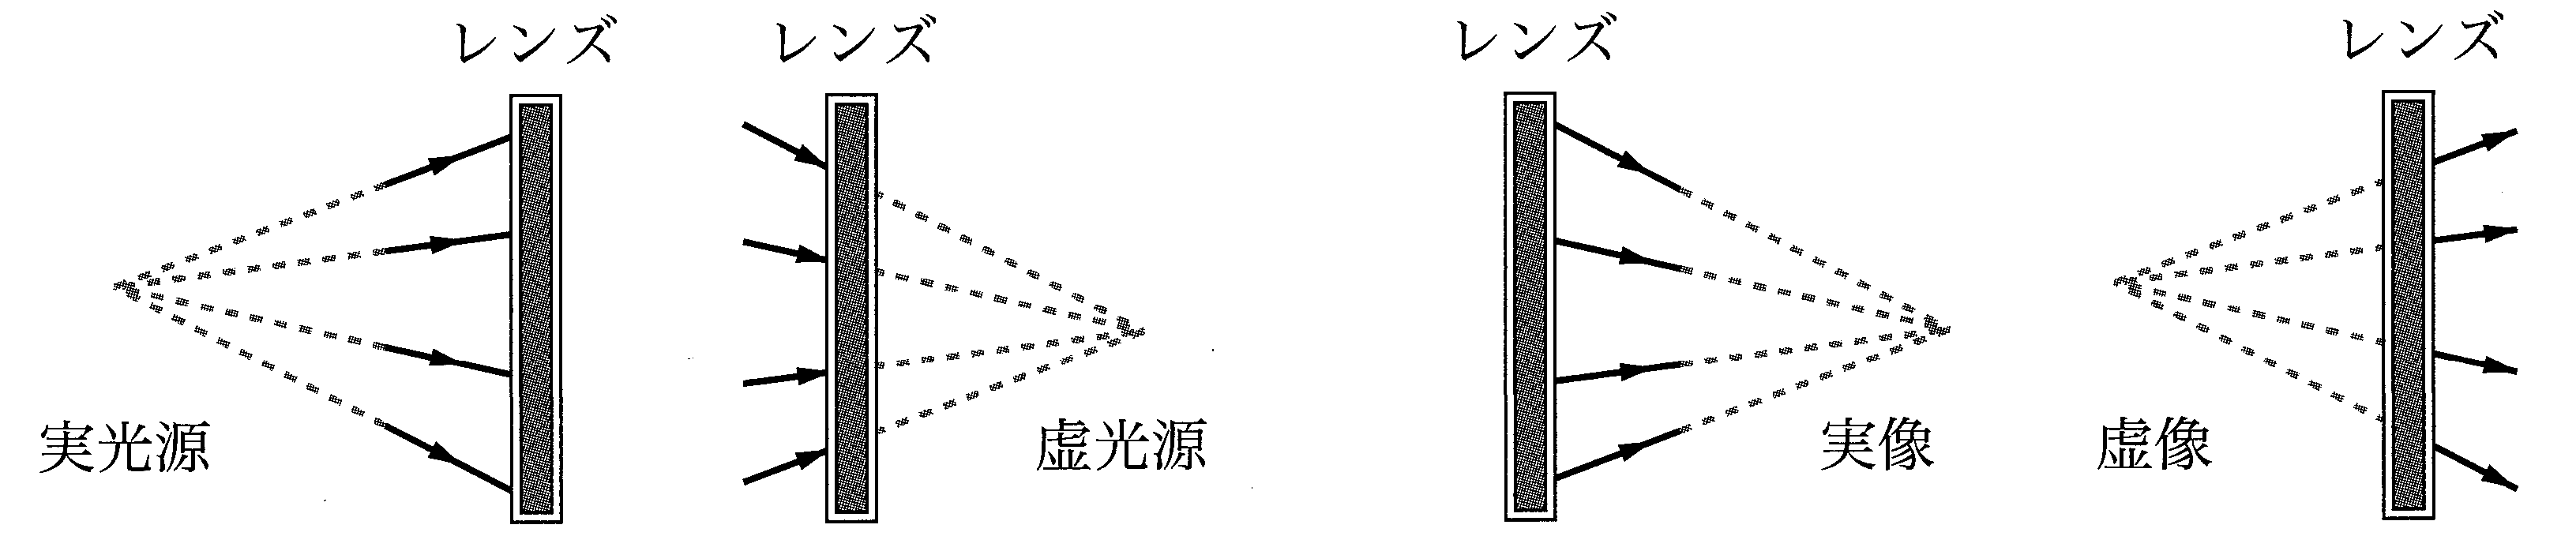
\includegraphics[width=130mm]{text2_p19_fig2.png}
\end{center}
\end{figure}

 レンズを通じて，入射する光が曲げられ，集光する位置が変化することを{\bf 写像}と呼ぶ．
 光源，像は1回の写像ごとに位置が定義されるもので，特に複数のレンズを組み合わせた光学系では，各写像に対し，入射する光が実際に存在する光源から出た光であるとは限らず，また，レンズを通過した光が一点に集光するとは限らない．
 
 \newpage
 \subsection{凹面鏡，凸面鏡}
 
 鏡によっても，光の集光，写像を五輪することができる．
 中央部がへこんでいる鏡を凹面鏡，出っ張っている鏡を凸面鏡と呼ぶ．
 
 凹面鏡に光軸に対して平行な光線をあてると，反射光は鏡の手前のある一点に集光する．
 この点を凹面鏡の焦点と呼び，凹面鏡から焦点までの距離を焦点距離と呼ぶ．
 また，焦点の位置に光源を置くと，光線の通り道は先ほどと逆になり，反射光は光軸と平行な光線群となる．
 
 凸面鏡に光軸に対して平行な光線をあてると，反射光は広がっていき，その光線を凸面鏡の奥側まで伸ばすと，直線は一点で交わる．
 この位置を凸面鏡の焦点と呼び，凸面鏡から焦点までの距離を焦点距離と呼ぶ．
 また，凸面鏡の奥側の焦点に集まるような光線を入射すると，反射光は光軸と平行な光線群となる． 
  \begin{figure}[h]
\begin{center}
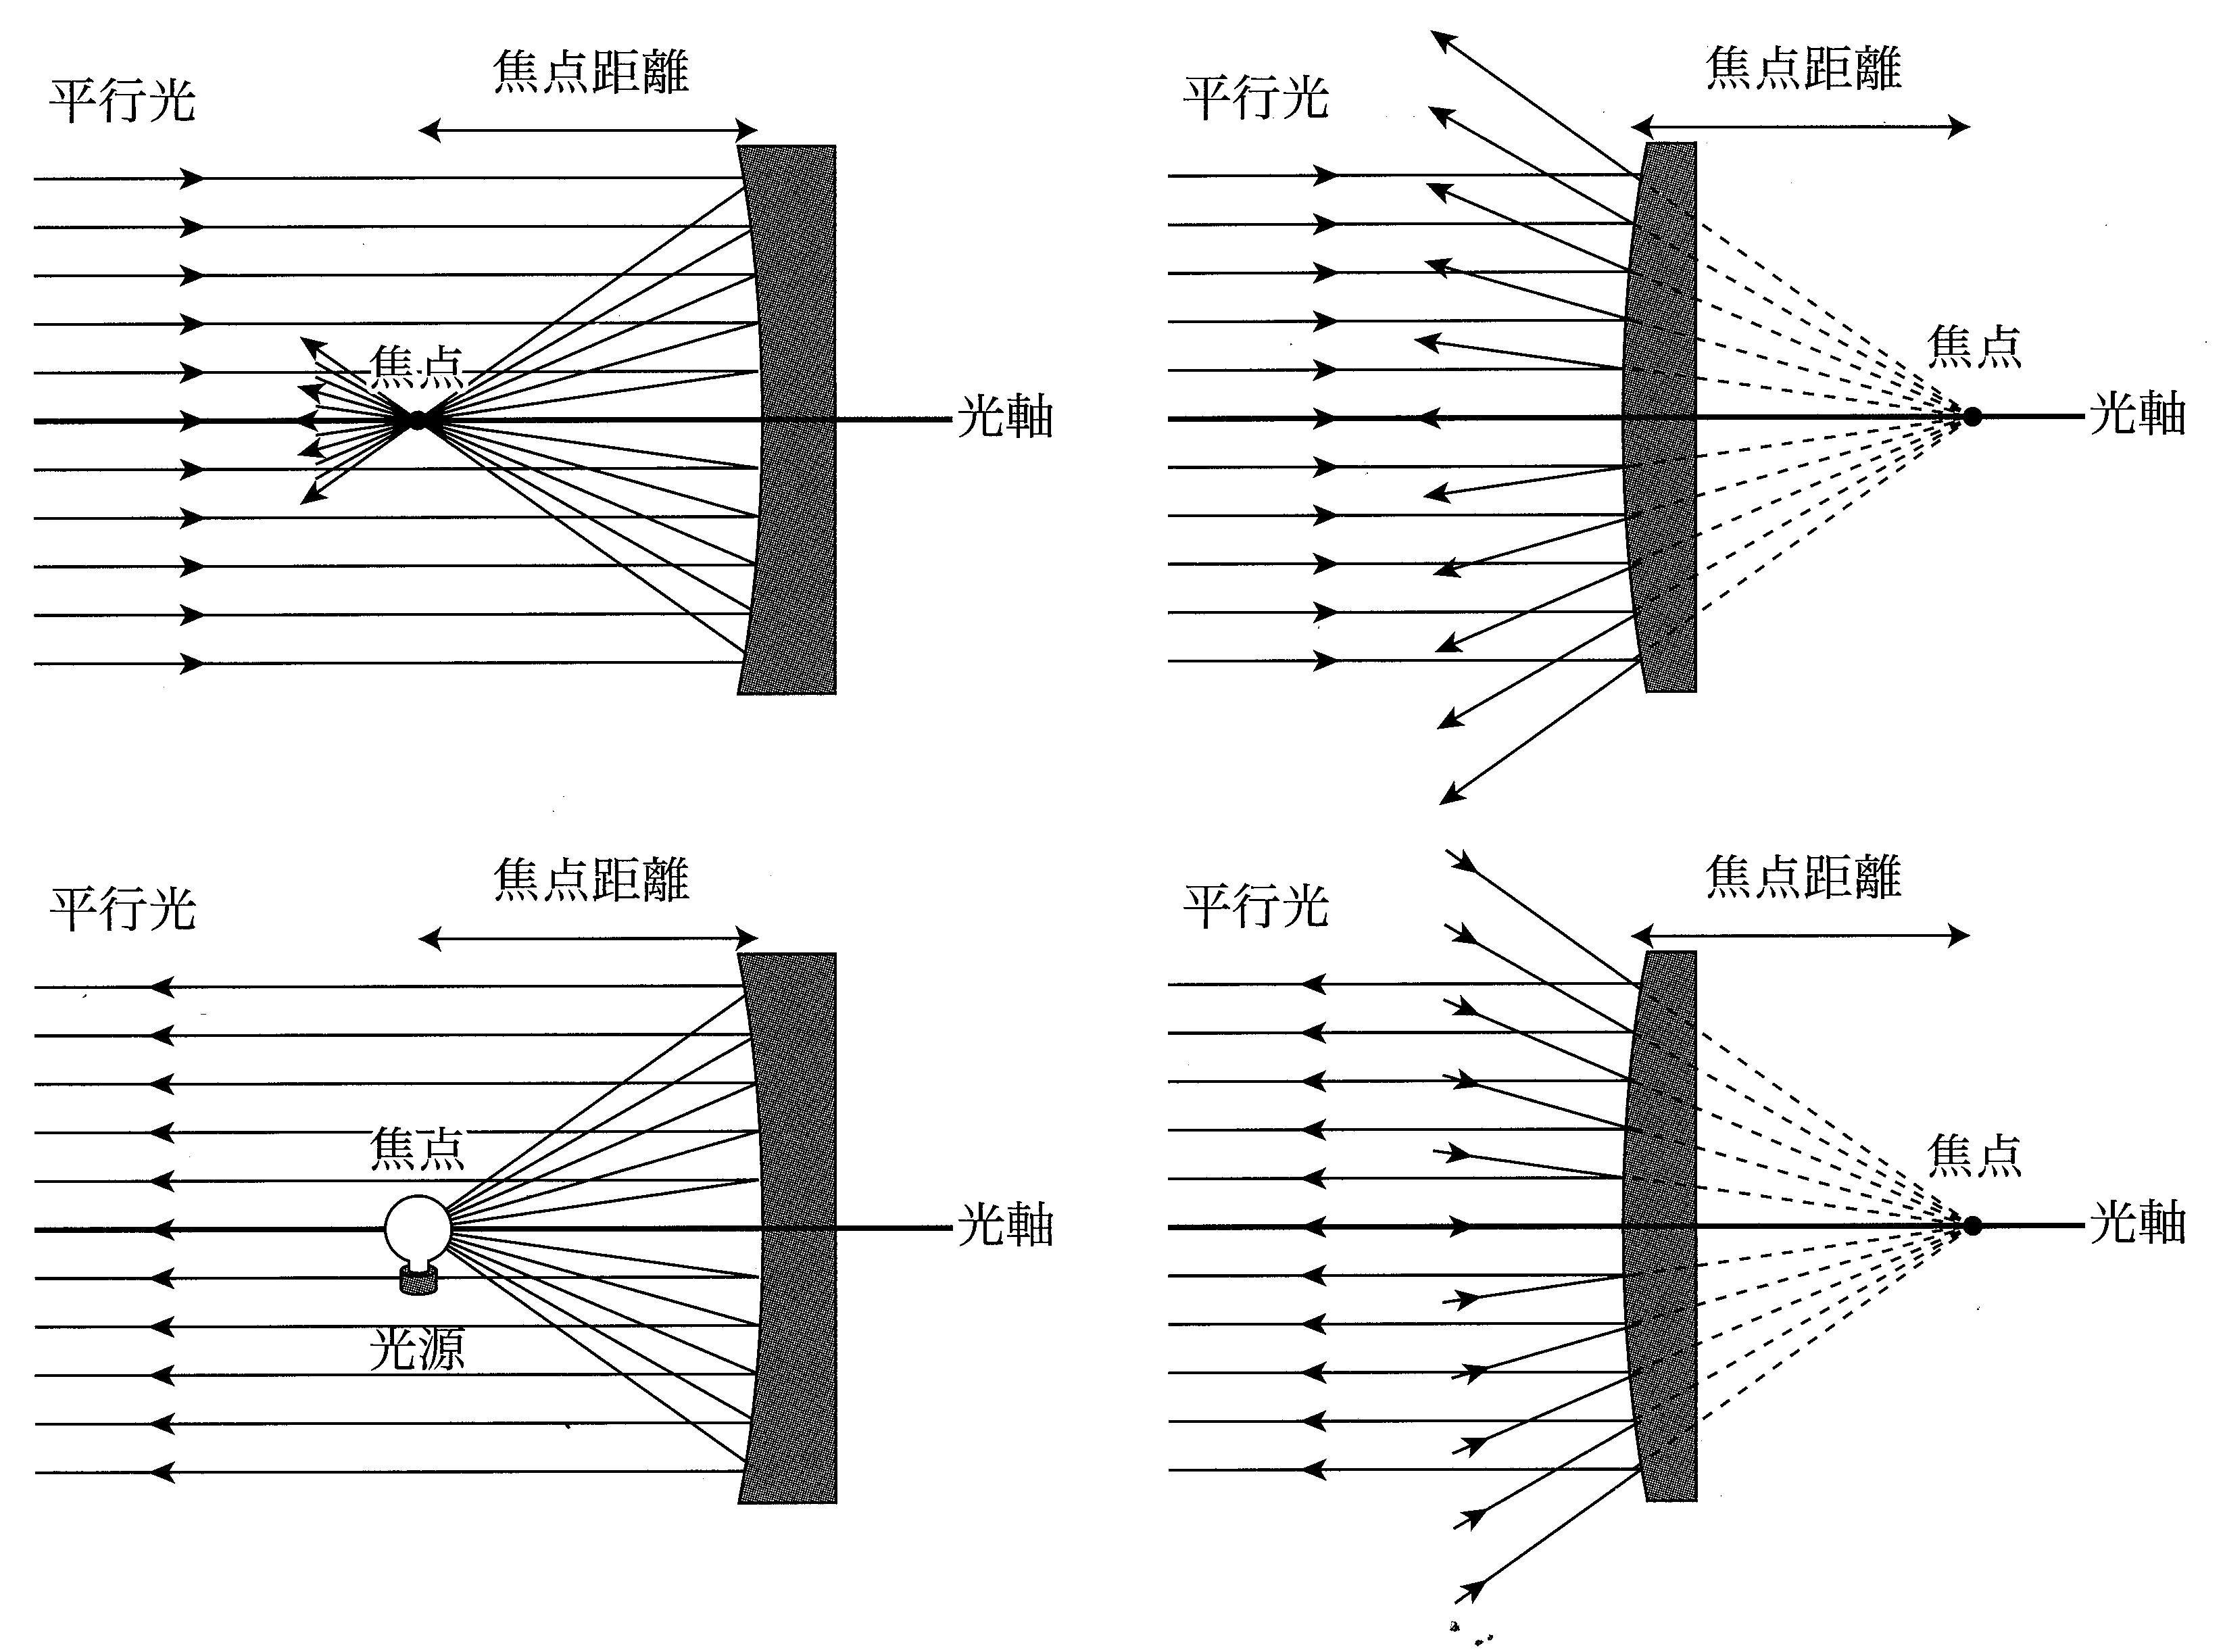
\includegraphics[width=130mm]{text2_p21_fig1.png}
\end{center}
\end{figure}


\newpage

\begin{figure}[h]
\begin{center}
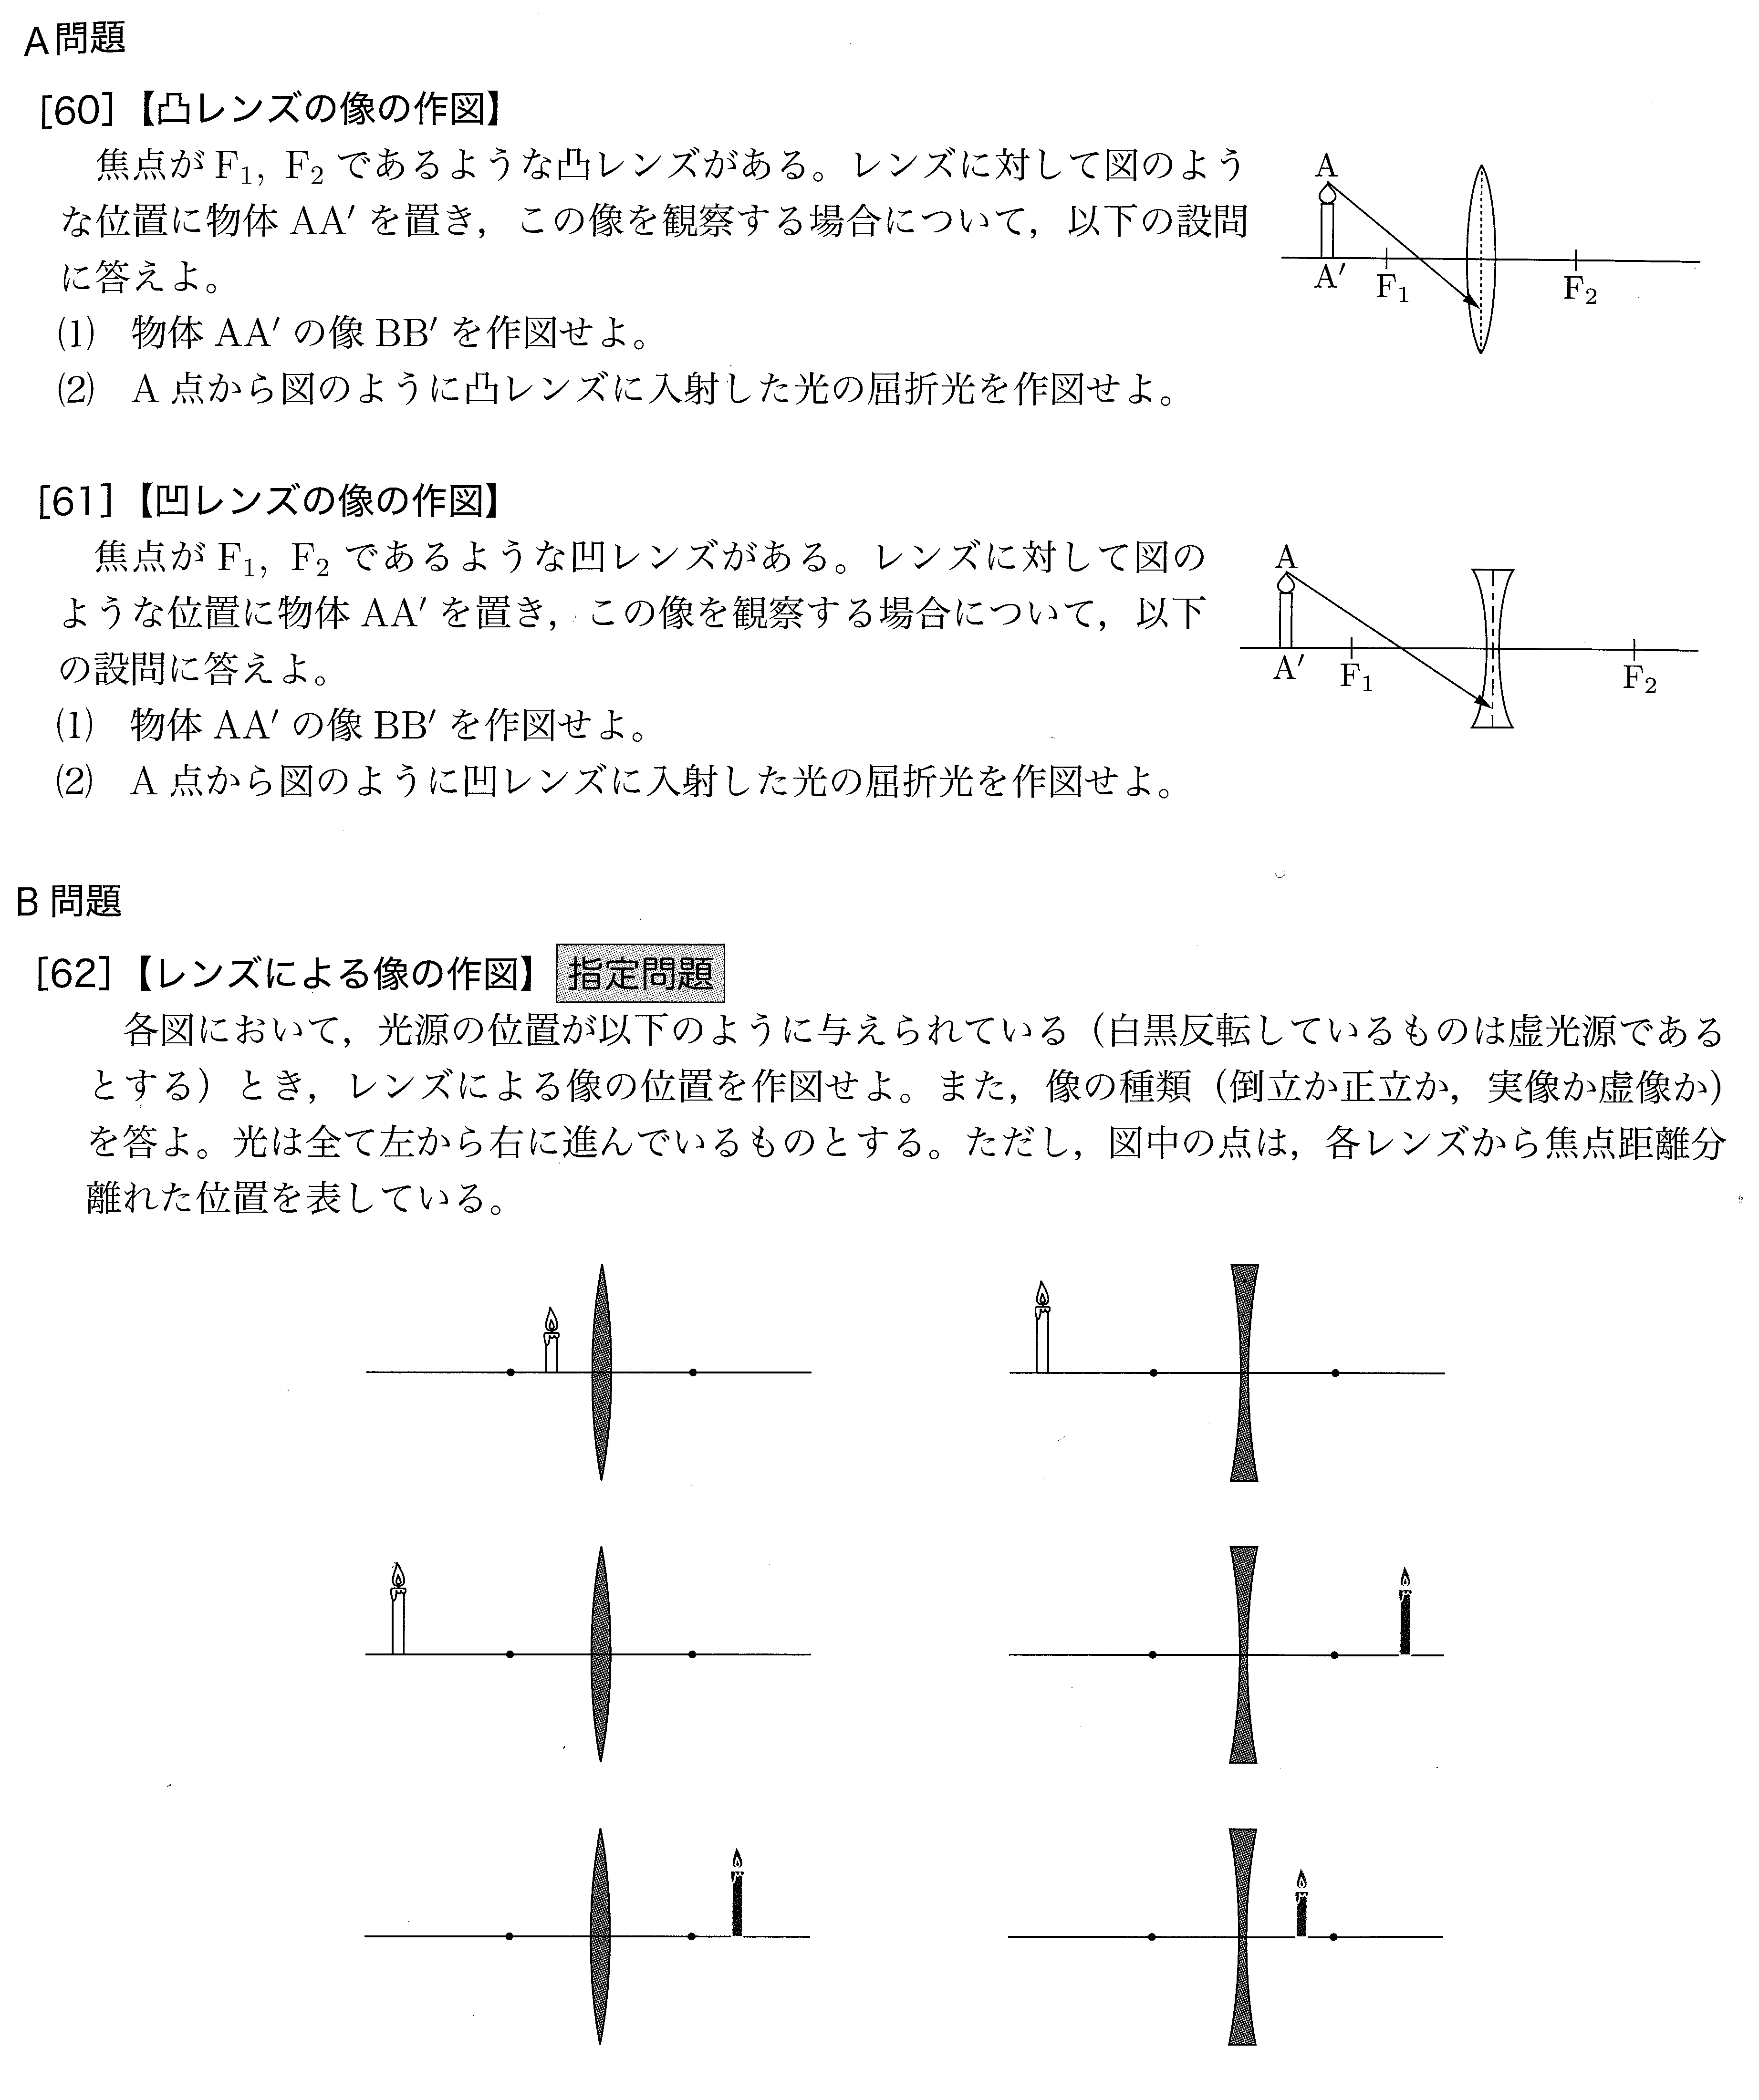
\includegraphics[width=170mm]{prob2_p11.png}
\vspace{150mm}
\end{center}
\end{figure}

\newpage

\begin{figure}[h]
\begin{center}
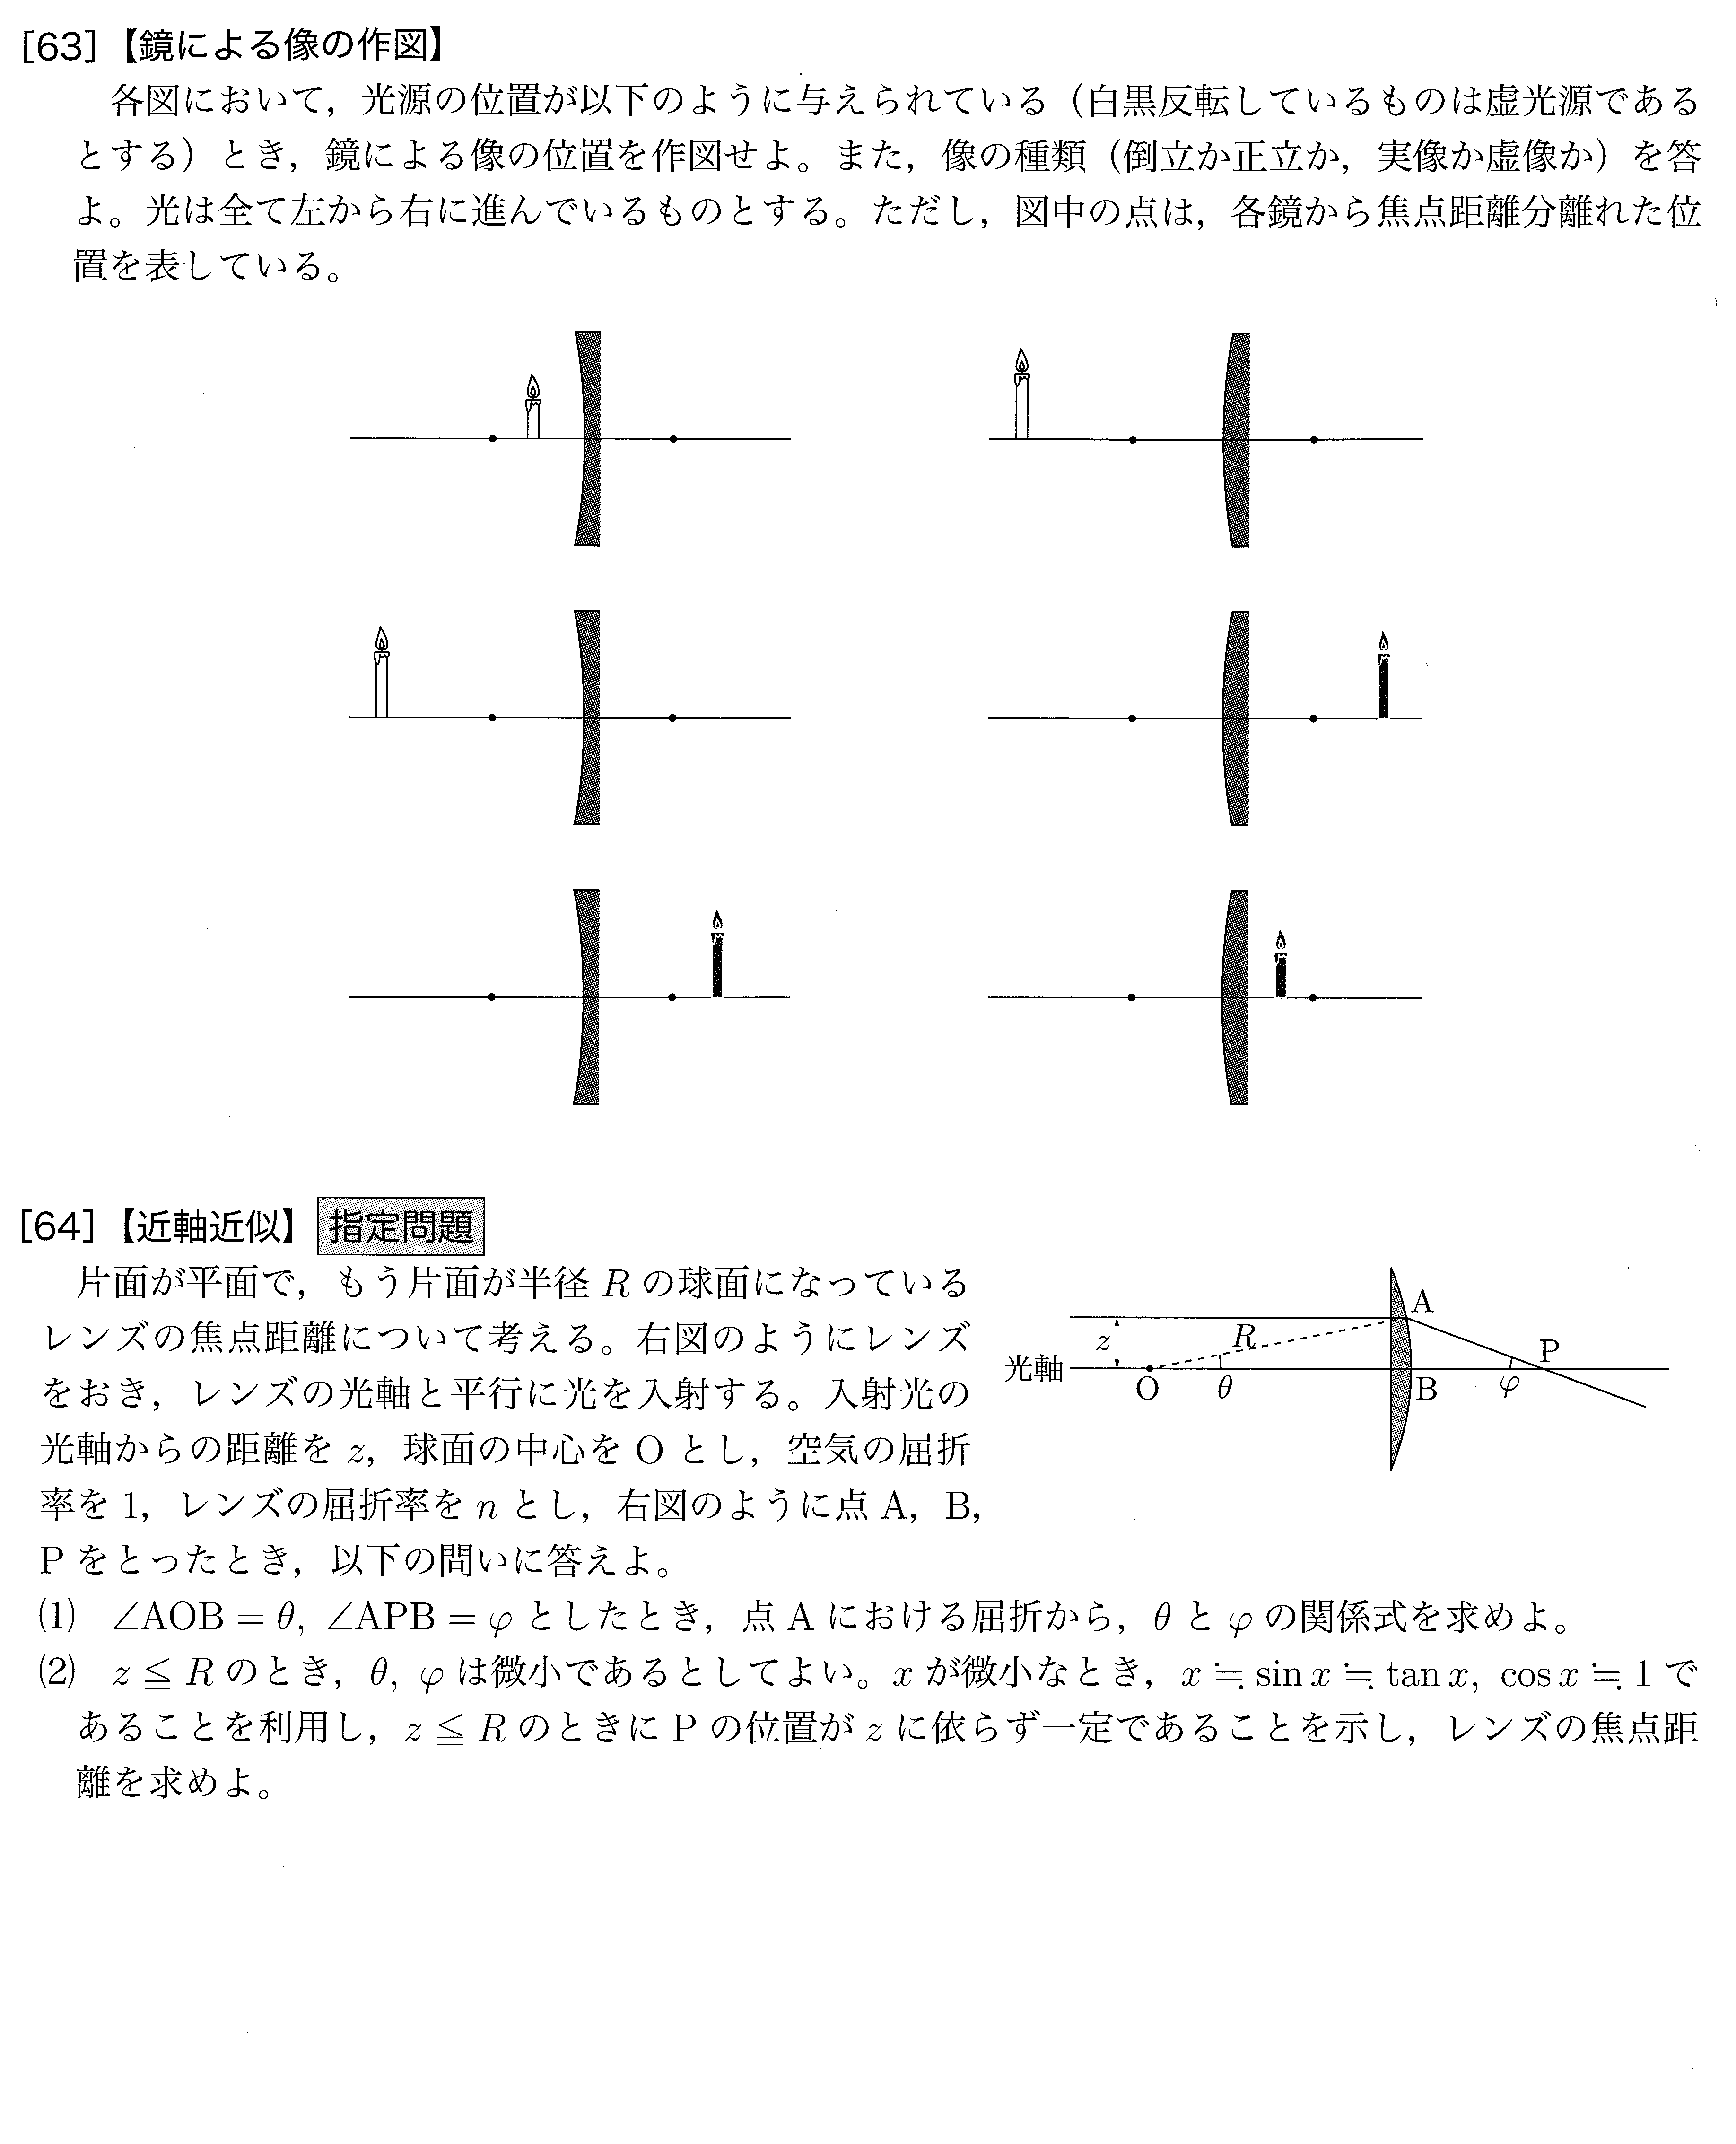
\includegraphics[width=170mm]{prob2_p12.png}
\vspace{150mm}
\end{center}
\end{figure}

\newpage

\begin{figure}[h]
\begin{center}
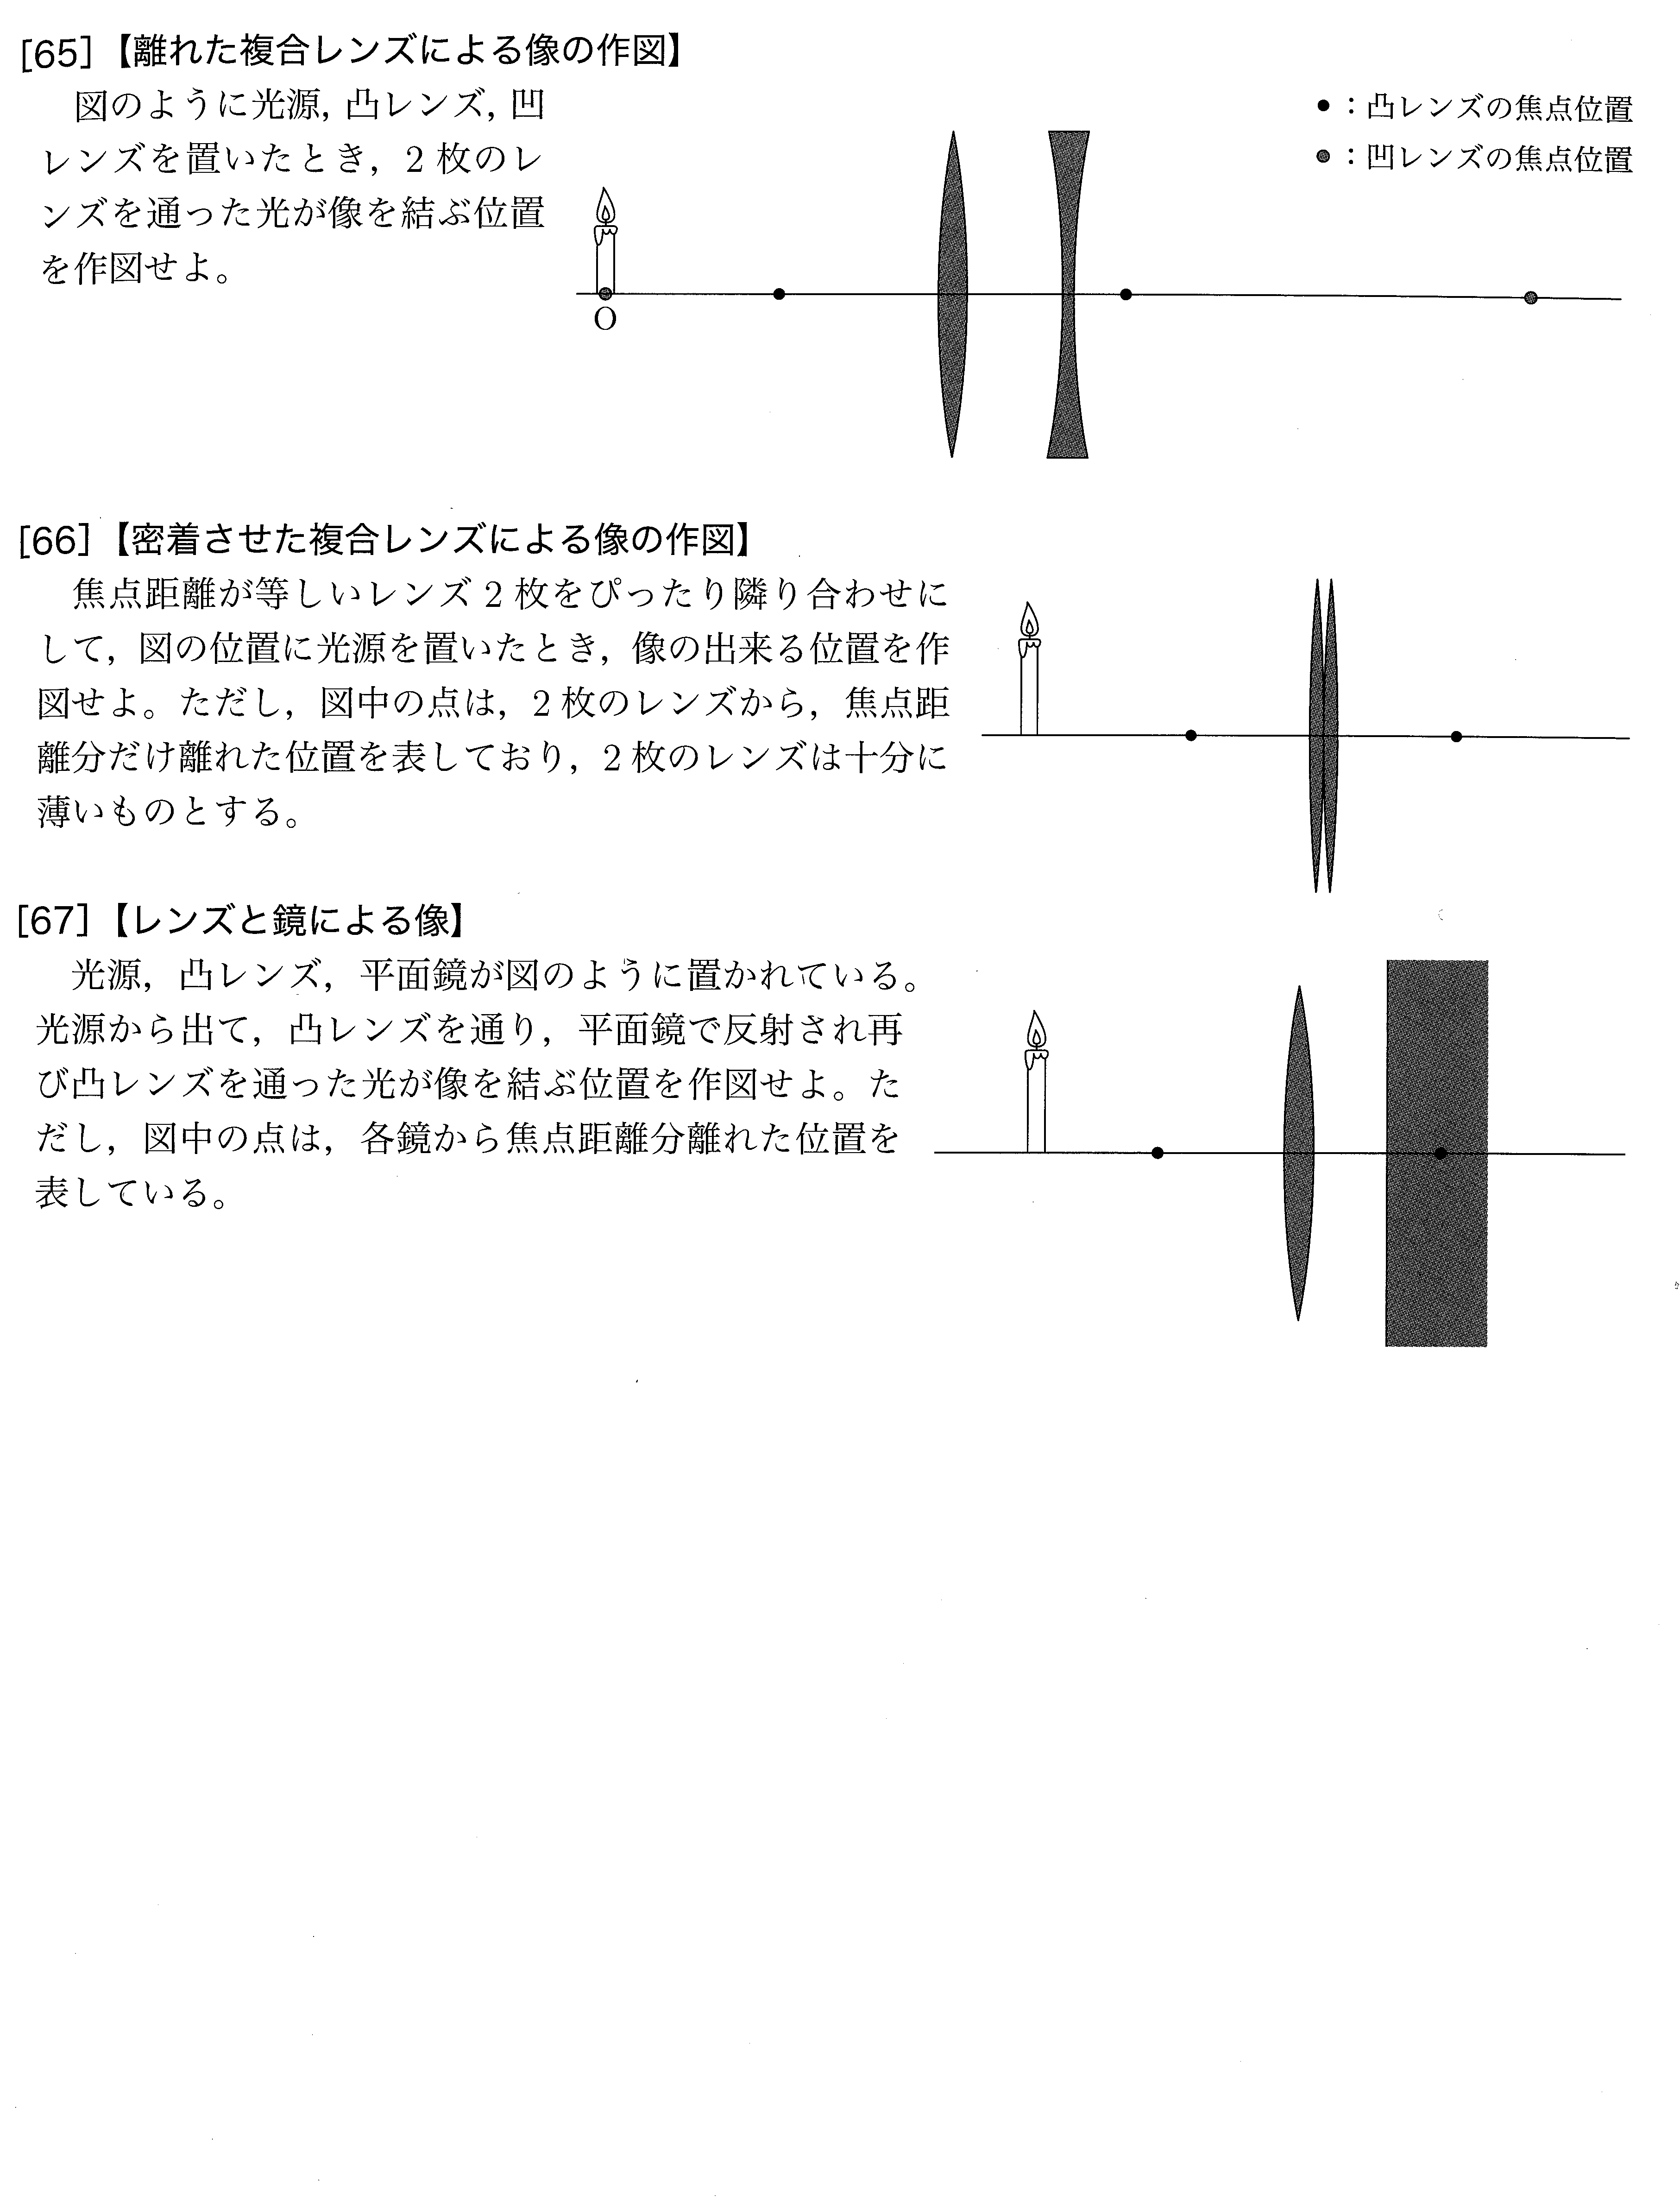
\includegraphics[width=170mm]{prob2_p13.png}
\vspace{150mm}
\end{center}
\end{figure}

\newpage

\begin{figure}[h]
\begin{center}
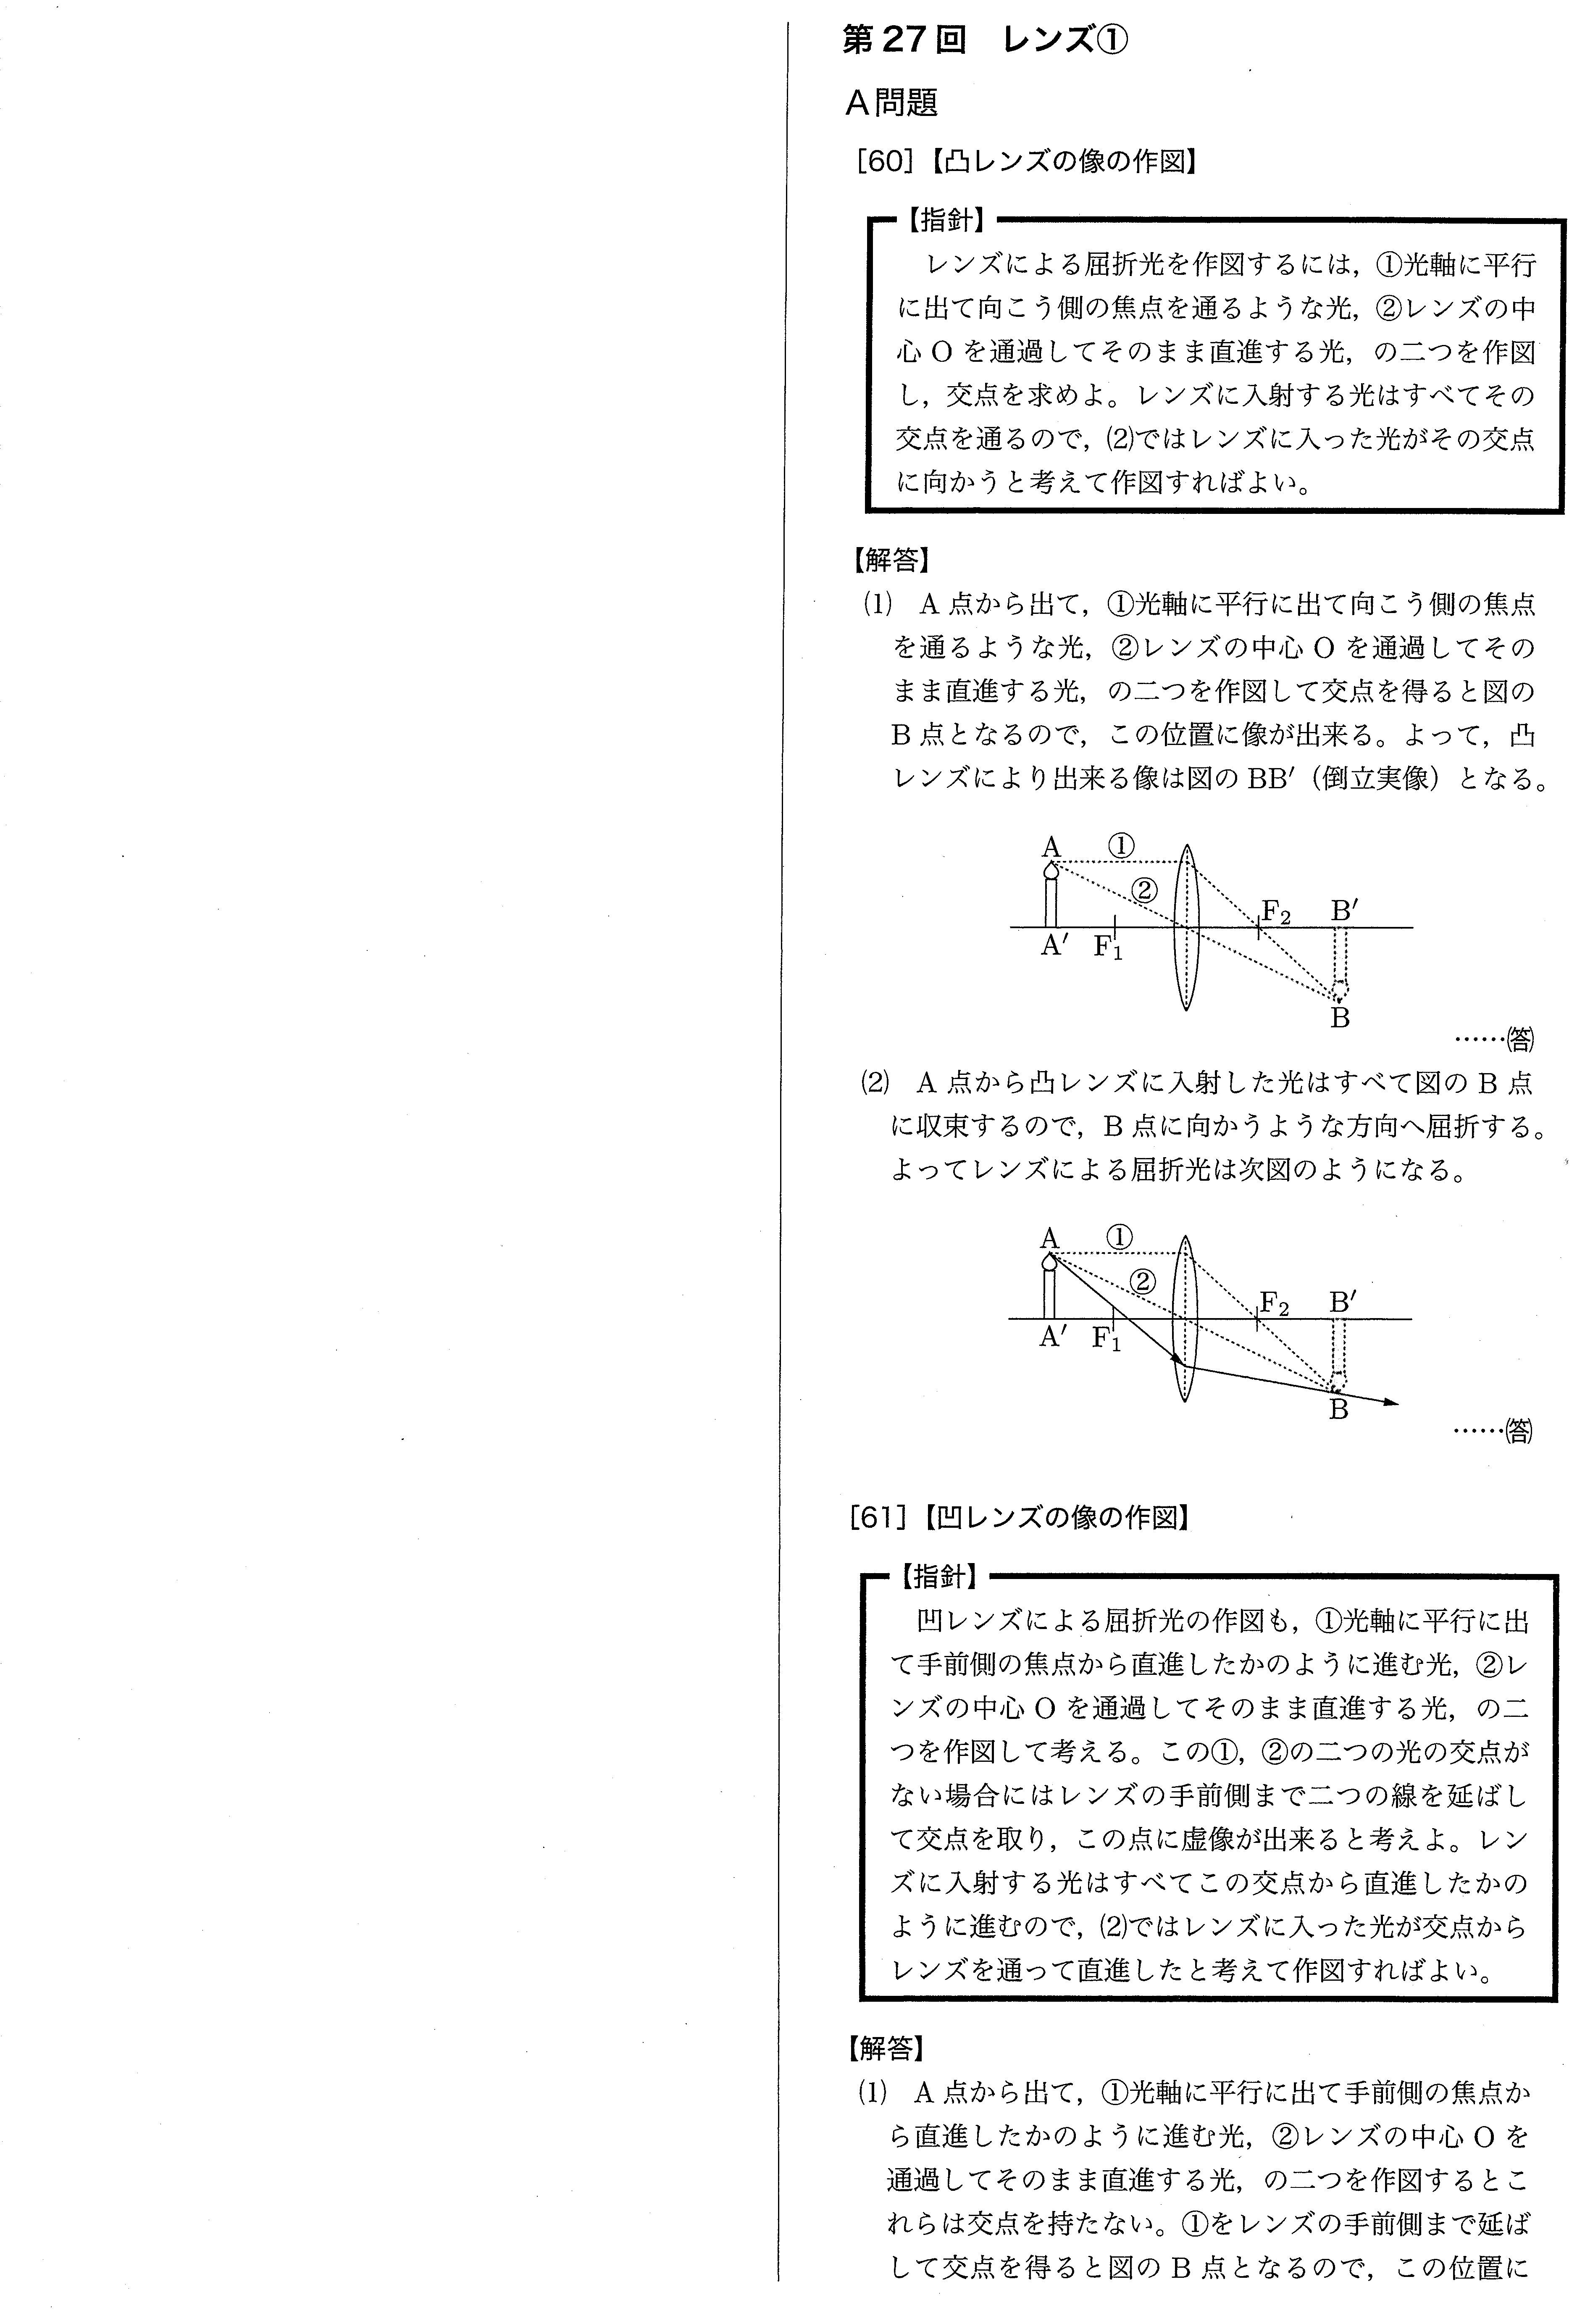
\includegraphics[width=170mm]{prob2_p83_2.png}
\vspace{150mm}
\end{center}
\end{figure}

\newpage

\begin{figure}[h]
\begin{center}
\includegraphics[width=170mm]{prob2_p84.png}
\vspace{150mm}
\end{center}
\end{figure}

\newpage

\begin{figure}[h]
\begin{center}
\includegraphics[width=170mm]{prob2_p85.png}
\vspace{150mm}
\end{center}
\end{figure}

\newpage

\begin{figure}[h]
\begin{center}
\includegraphics[width=170mm]{prob2_p86.png}
\vspace{150mm}
\end{center}
\end{figure}

 \ 
 
\newpage
\include{physics_ch28}
\include{physics_ch29}
 \ 
 
\newpage
\section{電位・電位によるエネルギー}

\subsection{電位}

空間中の電場の様子を表す方法として，電気力線を使う方法の他に，電位というものを利用する方法がある．
この電位を利用すると，電場が荷電粒子に対してなす仕事を考えることができる．

 \begin{wrapfigure}[10]{r}[5mm]{60mm}
  \centering
  \vspace{-10mm}
  \includegraphics[keepaspectratio,width=60mm]
  {text2_p31_fig1.png}
\end{wrapfigure}
\vspace{5mm}
$+1$[C]の点電荷を，電場に逆らってO点（基準点）からゆっくりP点まで動かすのに必要な仕事（エネルギー）が$V$[J]であるとき，P点の{\bf 電位}を$V$[V]（ボルト）と定義する．
この電位を利用すると，$+q$[C]の電荷を基準点Oから電位$V$[V]の点までゆっくりと動かすためには，$qV$[J]のエネルギーが必要である，と言える．
このことから，\mbox{\boldmath $+q$}{\bf [C]の電荷が電位}\mbox{\boldmath $V$}{\bf [V]の点で持つ位置エネルギーは}\mbox{\boldmath $U=qV$}{\bf [J]である．}

\vspace{5mm}
電位の基準点は，基本的にどこに取っても良いが，無限遠方，もしくは回路の問題では接地されている点（アース）を基準点に取ることが多い．

\vspace{8mm}
\begin{matome}{電荷の持つ位置エネルギー}
 \hspace{3mm} $+q$[C]の点電荷が$V$[V]の電位の点で持つ位置エネルギーは
 \[ U=qV \hspace{2mm}[{\rm J}] \]
 \end{matome}

この電位を用いて電場を考えると，{\bf 電場は電位の大きい方から小さい方へと向かっている}ので，電位は電荷にとっての高さのようなものだと考えれば良い．
すなわち，{\bf 正電荷は高電位$\rightarrow$ 低電位へ向かおうとし，負電荷は低電位$\rightarrow$ 高電位へと向かおうとする．}
また，電位の傾きが大きいほど受ける力は大きいので，{\bf 電位の傾きが電場の大きさに対応している．}

電場の様子に応じてさまざまな電位が存在するが，そのうち以下の2つを覚えておけば十分である．\\[5mm]

 \begin{wrapfigure}[15]{r}[5mm]{50mm}
  \centering
  \vspace{-5mm}
  \includegraphics[keepaspectratio,width=50mm]
  {text2_p32_fig1.png}
\end{wrapfigure}
$\MARU{1}$\hspace{2mm} {\bf 一様電場}

2つの金属板を距離$d$[m]だけ離して平行に配置し（これを{\bf 平行平板コンデンサー}という），各々を$+Q$[C]，$-Q$[C]に帯電させると，図のA$\rightarrow$Bへと向かう，平行かつ一様な電場$E$[N/C]が生じる．図から明らかに正に帯電したA側がより高電位となる．
図の$V-x$グラフの傾きが$E$であるから，AとBの電位差は
\[ \Delta V=Ed \]
で与えられる．
すなわち，{\bf 負に帯電した金属板よりも正に帯電した金属板の方が} \mbox{\boldmath $Ed$} {\bf [V]だけ電位が高い．}

$\MARU{1}$のグラフから分かるように，向きまで考慮すると電場と電位との間には，
\[ E=-\dfrac{dV}{dx} \hspace{2mm}[{\rm N/C}]\]
の関係がある．
この式から，電場の単位は[N/C]=[V/m]である．\\[5mm]

 \begin{wrapfigure}[25]{r}[5mm]{75mm}
  \centering
  \vspace{-5mm}
  \includegraphics[keepaspectratio,width=75mm]
  {text2_p32_fig2.png}
\end{wrapfigure}
$\MARU{2}$\hspace{2mm} {\bf 点電荷による電場}

原点に$+Q$[C]の点電荷が置かれているとき，座標$x$[m]$(>0)$における電場は$+x$方向に$E=k\dfrac{Q}{x^2}$[N/C]であるから，この点において$\dfrac{d}{dx}V(x)=-k\dfrac{Q}{x^2}$を満たすような$V(x)$[V]が電位である．
よって，この式の両辺を積分すると，
\[ V(x)=-\displaystyle \int k\dfrac{Q}{x^2}dx =k\dfrac{Q}{x} +C\]
となるが，この積分定数$C$の値は，電位の基準点をどこにするかによって決まる．

式が簡単になるように，{\bf 無限遠点を基準にする}，すなわち$x \rightarrow \infty$のとき$V(x)\rightarrow 0$となるように$C$の値をとると，
\[ V(x)=k\dfrac{Q}{x} \hspace{2mm} [{\rm V}] \]
と表される．$x<0$の場合も含めると，
\[ V(x)=k\dfrac{Q}{|x|} \hspace{2mm} [{\rm V}] \]
となり，点電荷からの距離を$r$[m]とすれば
\[ V(x)=k\dfrac{Q}{r} \hspace{2mm} [{\rm V}] \]
となる．
また，点電荷が複数ある場合には，その重ね合わせで電位を求めれば良い．

\begin{matome}{電場と電位}
\[ E=-\dfrac{dV}{dx} \hspace{2mm}[{\rm N/C}]\]
電場は高電位$\rightarrow$ 低電位を向く．
電位の傾きが電場の大きさに対応．
 \end{matome}
 
 \begin{matome}{一様電場・点電荷による電位}
\begin{description}
\item[\MARU{1}] 一様電場による電位\\
強さ$E$[N/C]，距離$d$[m]離れた2点間の電位差は$\Delta V=Ed$\hspace{2mm}[V]
\item[\MARU{2}] 点電荷による電位\\
$+Q$[C]の点電荷から距離$r$[m]の点における電位は無限遠点を基準として，$V=k\dfrac{Q}{r}$\hspace{2mm}[V]
\end{description}
 \end{matome}
 
 \newpage
 \subsection{導体の性質}
 
 金属のように電気をよく通すものを{\bf 導体}と呼び，逆にプラスチックのように電気を通さないものを{\bf 不導体}（もしくは{\bf 誘電体}）と呼ぶ．
 
  \begin{wrapfigure}[7]{r}[5mm]{50mm}
  \centering
  \vspace{-5mm}
  \includegraphics[keepaspectratio,width=50mm]
  {text2_p35_fig1.png}
\end{wrapfigure}
 導体，例えば金属の場合，その自由電子は金属内を自由に動き回れるため，電子が導体内で動くのにエネルギーを必要としない．
 このことから，{\bf 導体内の電位は一定}である．
 また，導体に外部から電場がかけられるとその電場によって速やかに電子が移動し，外部からかけられた電場を打ち消すことにより電子の移動が止まる．
 そのため，外部から{\bf 電場をかけても導体内には電場が生じない．}
 
 また，静電状態（電流が流れていない状態）の導体内部にもし電荷があると導体内部に電場が生じてしまうが，これは上で述べたことに反する．
 よって，{\bf 静電状態にある導体の内部には電荷が生じず，導体表面に電荷が現れる．}
 
 この性質を利用すると，例えば図(a)のように箔検電器を接地した金属製の箱で囲むことにより，外部から帯電したエボナイト棒を近づけても静電誘導は起こらない．
 また図(b)のように帯電した物体を接地した金属製の箱で覆うことにより，帯電体から出てくる電場を遮断することができる．
 このように，導体で囲むことによって内外の電場を遮断することを{\bf 静電遮蔽}という．
 \begin{figure}[h]
\begin{center}
\includegraphics[width=125mm]{text2_p35_fig2.png}
\end{center}
\end{figure}

 \newpage

\begin{figure}[h]
\begin{center}
\includegraphics[width=170mm]{prob2_p20.png}
\vspace{150mm}
\end{center}
\end{figure}

\newpage

\begin{figure}[h]
\begin{center}
\includegraphics[width=170mm]{prob2_p21.png}
\vspace{150mm}
\end{center}
\end{figure}

\newpage

\begin{figure}[h]
\begin{center}
\includegraphics[width=170mm]{prob2_p100_2.png}
\vspace{150mm}
\end{center}
\end{figure}

\newpage

\begin{figure}[h]
\begin{center}
\includegraphics[width=170mm]{prob2_p101.png}
\vspace{150mm}
\end{center}
\end{figure}

\newpage

\begin{figure}[h]
\begin{center}
\includegraphics[width=170mm]{prob2_p102.png}
\vspace{150mm}
\end{center}
\end{figure}

\newpage

\begin{figure}[h]
\begin{center}
\includegraphics[width=170mm]{prob2_p103.png}
\vspace{150mm}
\end{center}
\end{figure}

\newpage

\begin{figure}[h]
\begin{center}
\includegraphics[width=170mm]{prob2_p104.png}
\vspace{150mm}
\end{center}
\end{figure}

\newpage

\begin{figure}[h]
\begin{center}
\includegraphics[width=170mm]{prob2_p105_1.png}
\vspace{150mm}
\end{center}
\end{figure}

 \ 
 
\newpage
\include{physics_ch31}
 \ 
 
\newpage
\section{コンデンサー回路}

\subsection{キルヒホッフの第二法則}
全セクションで学んだコンデンサーと電池およびスイッチを導線でつなぐと様々な回路を作ることができるが，スイッチを開閉したときにコンデンサーにどのように電荷が蓄えられるかを考えるためには，{\bf 電荷保存の法則}と{\bf キルヒホッフの第二法則}とを組み合わせて考えていけば良い．

  \begin{wrapfigure}[12]{r}[5mm]{60mm}
  \centering
  \vspace{-5mm}
  \includegraphics[keepaspectratio,width=60mm]
  {text2_p40_fig1.png}
\end{wrapfigure}
電気回路において，導線中（導体中）の電位は必ず一定であるから，（急激な電荷の移動がなければ）{\bf 導線でつながっているところは必ず等電位になっている．}
そして，{\bf 電池や回路中の素子（コンデンサーや抵抗など）で電位が高くなったり低くなったりする．}
このとき，{\bf 回路中の任意の閉ループをひと回りした場合には，必ず同じ電位に戻ってくる．}
これを{\bf キルヒホッフの第二法則}という．\\[5mm]

回路のキルヒホッフの法則は，導線部分を平坦な道，素子を坂道に例えて捉えるとわかりやすい．

コンデンサーを組み合わせて作られた回路で，各コンデンサーに蓄えられる電荷を求めるためには，各コンデンサーに蓄えられる電荷を文字で置き，回路のキルヒホッフ第二法則を立てればよい．

\begin{matome}{キルヒホッフの第二法則}
 \hspace{3mm} 回路上の任意の閉ループをひと回りした場合には，必ず同じ電位に戻ってくる．
 \end{matome}
 
   \begin{wrapfigure}[7]{r}[5mm]{50mm}
  \centering
  \vspace{-5mm}
  \includegraphics[keepaspectratio,width=50mm]
  {text2_p40_fig2.png}
\end{wrapfigure}
また，電荷は電子の過不足により生じるものであるから，例えば図のように{\bf 他の回路から離れているような部分回路ではその内部で電子が移動するのみであるから，その全電気量は不変である．}
これを{\bf 電荷保存の法則}という．

コンデンサー回路を考えていくときは ，このような，他の回路から浮いている部分（孤立した部分）を発見し，その部分に電荷保存の法則を考えていくことが大切である．

コンデンサーでは，{\bf 向かい合う極板には必ず正負逆，大きさが同じ電荷が蓄えられるが，正の電荷が蓄えられている側がより高電位}である．

\subsection{コンデンサー回路}
キルヒホッフ第二法則と電荷保存の法則を組み合わせると，様々なコンデンサー回路の電荷分布の変化を計算することができるが，その方針をここで再度まとめておく．

\begin{matome}{コンデンサー回路}
\begin{description}
\item[\MARU{1}] 各コンデンサーの帯電量を文字$+q$\hspace{1mm}[C]，$-q$\hspace{1mm}[C]などでおく．
\item[\MARU{2}] 回路の浮いている部分について，電荷保存の法則を適用する．
\item[\MARU{3}] 帯電量$+q$\hspace{1mm}[C]側の極板の方が$\dfrac{q}{C}$\hspace{1mm}[V]だけ電位が高いことを利用して，キルヒホッフ第二法則を立てる．
\end{description}
 \end{matome}

\subsection{複合極板コンデンサー}
今までは極板が2枚の平行平板コンデンサーを扱ってきたが，この極板間に導体を挟んだり，すき間の一部分にのみ誘電体を挿入するなどしたコンデンサーも存在する．
このようなコンデンサーを扱う場合には，以下のようにコンデンサーを書き換えて扱えばよい．

$\MARU{1}$\hspace{2mm} 導体を挟んだコンデンサー：{\bf 導体部を導線だとみなして}2つのコンデンサーを分解する
 \begin{figure}[h]
\begin{center}
\includegraphics[width=80mm]{text2_p42_fig1.png}
\end{center}
\end{figure}

$\MARU{2}$\hspace{2mm} 誘電体を挟んだコンデンサー：{\bf 誘電体部分を別のコンデンサーだとみなす}
 \begin{figure}[h]
\begin{center}
\includegraphics[width=80mm]{text2_p42_fig2.png}
\end{center}
\end{figure}

$\MARU{3}$\hspace{2mm} 多極板コンデンサー：{\bf 間に導線を仮想}して複数のコンデンサーに分解する
 \begin{figure}[h]
\begin{center}
\includegraphics[width=80mm]{text2_p43_fig1.png}
\end{center}
\end{figure}

$\MARU{4}$\hspace{2mm} 並列型に挿入された誘電体：横に分けて{\bf 並列型コンデンサー}だとみなす
 \begin{figure}[h]
\begin{center}
\includegraphics[width=80mm]{text2_p43_fig2.png}
\end{center}
\end{figure}

複雑なコンデンサーは単純なコンデンサーの合成だとみなして回路を書き換え，コンデンサー回路の考え方に従って電荷分布を求める．

  \newpage

\begin{figure}[h]
\begin{center}
\includegraphics[width=170mm]{prob2_p25.png}
\vspace{150mm}
\end{center}
\end{figure}

\newpage

\begin{figure}[h]
\begin{center}
\includegraphics[width=170mm]{prob2_p26.png}
\vspace{150mm}
\end{center}
\end{figure}

\newpage

\begin{figure}[h]
\begin{center}
\includegraphics[width=170mm]{prob2_p27.png}
\vspace{150mm}
\end{center}
\end{figure}

\newpage

\begin{figure}[h]
\begin{center}
\includegraphics[width=170mm]{prob2_p111_2.png}
\vspace{150mm}
\end{center}
\end{figure}

\newpage

\begin{figure}[h]
\begin{center}
\includegraphics[width=170mm]{prob2_p112.png}
\vspace{150mm}
\end{center}
\end{figure}

\newpage

\begin{figure}[h]
\begin{center}
\includegraphics[width=170mm]{prob2_p113.png}
\vspace{150mm}
\end{center}
\end{figure}

\newpage

\begin{figure}[h]
\begin{center}
\includegraphics[width=170mm]{prob2_p114.png}
\vspace{150mm}
\end{center}
\end{figure}

\newpage

\begin{figure}[h]
\begin{center}
\includegraphics[width=170mm]{prob2_p115.png}
\vspace{150mm}
\end{center}
\end{figure}

\newpage

\begin{figure}[h]
\begin{center}
\includegraphics[width=170mm]{prob2_p116.png}
\vspace{150mm}
\end{center}
\end{figure}

\newpage

\begin{figure}[h]
\begin{center}
\includegraphics[width=170mm]{prob2_p117.png}
\vspace{150mm}
\end{center}
\end{figure}

\newpage

\begin{figure}[h]
\begin{center}
\includegraphics[width=170mm]{prob2_p118.png}
\vspace{150mm}
\end{center}
\end{figure}

\newpage

\begin{figure}[h]
\begin{center}
\includegraphics[width=170mm]{prob2_p119.png}
\vspace{150mm}
\end{center}
\end{figure}
\include{physics_ch33}
 \ 
 
\newpage
\section{キルヒホッフの法則}

\subsection{キルヒホッフの第一法則}
\begin{wrapfigure}[8]{r}[5mm]{60mm}
  \centering
  \vspace{-5mm}
  \includegraphics[keepaspectratio,width=60mm]
  {text2_p51_fig1.png}
\end{wrapfigure}
ここまでは回路に枝分かれのないものを取り扱ってきたが，枝分かれのある回路について扱うときには以下の{\bf キルヒホッフの第一法則}を考える必要がある．
電流は電荷の流れであり，電荷はコンデンサー極板上にしか長時間滞在することはできない．
そのため，{\bf 回路の導線の分岐点に流れ込む電流の総量と，その点から流れ出て行く電流の総量とは必ず等しくなる．}これを{\bf キルヒホッフの第一法則}という．

このキルヒホッフの第一法則と，キルヒホッフの第二法則とを併用することにより，抵抗と電池により構成された回路に流れる電流を計算することができる．

\begin{matome}{キルヒホッフの法則}
 {\bf 第一法則}\\
 \hspace{3mm} 回路の分岐点に流れ込む電気量と流れ出て行く電気量とは必ず等しくなる\\
 {\bf 第二法則}\\
\hspace{3mm} 回路の任意の閉ループにおいて，起電力の代数和は電圧降下の代数和に等しい
 \end{matome}
 
各導線を流れる電気量を未知数として設定していく際に，先にキルヒホッフ第一法則を適用することで，未知変数の数が減るので楽になることが多い．

\subsection{抵抗の直列接続と並列接続} 
複数の抵抗を連結させたものをあたかも1つの抵抗であるかのように扱うことができる．
これを抵抗の合成といい，これをうまく用いると複雑なキルヒホッフの法則の式を計算せずに流れる電流を計算できる．\\[5mm]

\begin{wrapfigure}[12]{r}[5mm]{50mm}
  \centering
  \vspace{-5mm}
  \includegraphics[keepaspectratio,width=50mm]
  {text2_p52_fig1.png}
\end{wrapfigure}
$\MARU{1}$\hspace{2mm} {\bf 抵抗の直列接続 $\cdots$すべての抵抗に\underline {同じ電流}が流れる}

$R_1[\Omega],R_2[\Omega],R_3[\Omega]$の3つの抵抗を図のように直列に接続する．
この抵抗の両端に電流$I$[A]が流れたとき，各抵抗には$R_1I$[V],$R_2I$[V],$R_3I$[V]の電位差が生じ，ab間の電位差は
\[V_{\rm ab}=R_1I+R_2I+R_3I=(R_1+R_2+R_3)I \hspace{2mm} [{\rm V}] \]
である．
これを図のように1つの合成抵抗$R [\Omega]$であるとみなすと，
\[V_{\rm ab}=RI\hspace{2mm} [{\rm V}] \]
と書ける．
これより，この3つの抵抗を直列接続した場合は，
\[ \mbox{\boldmath$R=R_1+R_2+R_3 \hspace{2mm} [\Omega]$} \]
の合成だとみなすことができる．
また，各抵抗における電圧降下の比は
\[ R_1I:R_2I:R_3I=R_1:R_2:R_3\]
であり，抵抗値の比となる．\\[5mm]

\begin{wrapfigure}[12]{r}[5mm]{50mm}
  \centering
  \vspace{-5mm}
  \includegraphics[keepaspectratio,width=50mm]
  {text2_p52_fig2.png}
\end{wrapfigure}
$\MARU{2}$\hspace{2mm} {\bf 抵抗の並列接続 $\cdots$すべての抵抗に\underline {同じ電圧}がかかる}

$R_1[\Omega],R_2[\Omega],R_3[\Omega]$の3つの抵抗を図のように並列に接続する．
この抵抗の両端ab間に電圧$V_{\rm ab}$[V]がかかっているとき，各抵抗には
\[\dfrac{V_{\rm ab}}{R_1} [A],\hspace{3mm} \dfrac{V_{\rm ab}}{R_2} [A],\hspace{3mm} \dfrac{V_{\rm ab}}{R_3} [A]\]
の電流が流れる．
キルヒホッフの第一法則より，端子aに流れ込む電気量$I$[A]は
\[I=\dfrac{V_{\rm ab}}{R_1}+\dfrac{V_{\rm ab}}{R_2}+\dfrac{V_{\rm ab}}{R_3}=\left( \dfrac{1}{R_1} +\dfrac{1}{R_2} +\dfrac{1}{R_3} \right) V_{\rm ab} \hspace{2mm} [{\rm A}]\]
である．
これを図のように1つの合成抵抗$R[\Omega]$であるとみなすと，
\[ V_{\rm ab}=RI\hspace{2mm} [{\rm V}] \hspace{2mm}\Leftrightarrow \hspace{2mm}I=\dfrac{V_{\rm ab}}{R} \hspace{2mm}[{\rm A}] \]
と書ける．
これより，この3つの抵抗を並列接続した場合は，
\[ \mbox{\boldmath$\dfrac{1}{R}=\dfrac{1}{R_1}+\dfrac{1}{R_2}+\dfrac{1}{R_3} $} \]
を満たす$R[\Omega]$の合成抵抗だとみなすことができる．
また，各抵抗に流れ込む電気量の比は
\[ \dfrac{V_{\rm ab}}{R_1}:\dfrac{V_{\rm ab}}{R_2}:\dfrac{V_{\rm ab}}{R_3}=\dfrac{1}{R_1}:\dfrac{1}{R_2}:\dfrac{1}{R_3}\]
であり，抵抗値の逆数の比となる．

\begin{matome}{合成抵抗}
 \hspace{3mm} 抵抗の{\bf 直列}接続：合成抵抗値は各抵抗値の{\bf 単純和} \hspace{18mm}$R=R_1+R_2+R_3$\\
\hspace{3mm} 抵抗の{\bf 並列}接続：合成抵抗値の{\bf 逆数}は各抵抗値の{\bf 逆数の和} \hspace{5mm}$\dfrac{1}{R}=\dfrac{1}{R_1}+\dfrac{1}{R_2}+\dfrac{1}{R_3}$
 \end{matome}

\subsection{電流計・電圧計}
\begin{wrapfigure}[8]{r}[5mm]{60mm}
  \centering
  \vspace{-5mm}
  \includegraphics[keepaspectratio,width=60mm]
  {text2_p53_fig1.png}
\end{wrapfigure}

$\MARU{1}$\hspace{2mm} {\bf 電流計}

電流計は，電流の流れる導線が磁場中で電磁力と呼ばれる力を受けることを利用して電流の大きさを測定する装置であり，電流計を通過していく電流の大きさを測定することができる．
電流計には多大な電流が流入すると電流計が破壊されるので，これを防ぐためにその内部に内部抵抗がメーターに対して直列に取り付けられている．
電流計はAを$\bigcirc$で囲んだ記号で表すが，図のように{\bf 内部抵抗とメーターの2つに分けて書き直して考える}とよい．

電流計を用いて図のa点を流れる電気量を測定したい場合にはa点に電流計を挿入すればよい．
しかし，電流計の内部抵抗が大きいと通過していく電気量が変化してしまう．
そのため，{\bf 電流計の内部抵抗は極めて小さくなければならない．}\\[5mm]

$\MARU{2}$\hspace{2mm} {\bf 電圧計}

電流計において，内部抵抗の値$r[\Omega]$が既知であれば，流れる電気量$I$[A]を用いて電流計にかかる電圧$V=rI$[V]を計算できるから，{\bf 電流計は電圧計として利用することができ，}電圧計と電流計とはほぼ同じ作りになっている．
ただし，以下に述べるように，電流計と電圧計とではその測定方法および内部抵抗が異なる．

\begin{wrapfigure}[5]{r}[5mm]{70mm}
  \centering
  \vspace{-5mm}
  \includegraphics[keepaspectratio,width=70mm]
  {text2_p53_fig2.png}
\end{wrapfigure}
右図の回路において，図のab点間の電位差を測定したい場合には，ab点間に電圧計を接続すればよい．
しかし，電圧計の内部抵抗が小さいと電圧計に電流が流れ込んでしまうため，電流分布が変化し，測定すべき電位差が変化してしまう．
そのため，{\bf 電圧計の内部抵抗は極めて大きくなければならない．}

\subsection{ホイートストンブリッジ}
\begin{wrapfigure}[8]{r}[5mm]{40mm}
  \centering
  \vspace{-5mm}
  \includegraphics[keepaspectratio,width=40mm]
  {text2_p55_fig1.png}
\end{wrapfigure}

未知抵抗の抵抗値を精密に測定するためには以下に述べるホイートストンブリッジや，これを応用したメートルブリッジが用いられる．
ホイートストンブリッジは，抵抗値$R_1[\Omega]$，$R_2[\Omega]$，$R_3[\Omega]$，$R_4[\Omega]$の4つの抵抗を，検流計G，電池Eとともに図のように接続した回路である．
{\bf 検流計Gに電流が流れない場合は，}
\[R_1:R_2=R_3:R_4\]
{{\bf の関係が成立する．}

\begin{matome}{ホイートストンブリッジ}
 \hspace{3mm} 検流計Gに電流が流れない場合は，$R_1:R_2=R_3:R_4$の関係が成立する．
 \end{matome}
 
   \newpage

\begin{figure}[h]
\begin{center}
\includegraphics[width=170mm]{prob2_p31.png}
\vspace{150mm}
\end{center}
\end{figure}

\newpage

\begin{figure}[h]
\begin{center}
\includegraphics[width=170mm]{prob2_p32.png}
\vspace{150mm}
\end{center}
\end{figure}

\newpage

\begin{figure}[h]
\begin{center}
\includegraphics[width=170mm]{prob2_p124.png}
\vspace{150mm}
\end{center}
\end{figure}

\newpage

\begin{figure}[h]
\begin{center}
\includegraphics[width=170mm]{prob2_p125.png}
\vspace{150mm}
\end{center}
\end{figure}

\newpage

\begin{figure}[h]
\begin{center}
\includegraphics[width=170mm]{prob2_p126.png}
\vspace{150mm}
\end{center}
\end{figure}

\newpage

\begin{figure}[h]
\begin{center}
\includegraphics[width=170mm]{prob2_p127.png}
\vspace{150mm}
\end{center}
\end{figure}

 \ 
 
\newpage
\include{physics_ch35}
 \ 
 
\newpage
\include{physics_ch36}
 \ 
 
\newpage
\section{荷電粒子の運動}

\subsection{ローレンツ力}
電流の流れている導線は，周りの磁場から力を受けるが，これは電流の担い手として導線の中を{\bf 移動している電子が磁場から力を受ける}からである．
磁場中を運動する荷電粒子が，磁場から受ける力を{\bf ローレンツ力}という．

 \begin{wrapfigure}[6]{r}[5mm]{50mm}
  \centering
  \vspace{-5mm}
  \includegraphics[keepaspectratio,width=50mm]
  {text2_p66_fig1.png}
\end{wrapfigure}
電気量の大きさが$q$[C]の荷電粒子が，大きさ$B$[T]の{\bf 磁束密度に対して垂直な速度成分}\mbox{\boldmath$v$} {\bf [m/s]}を持っているとき，この荷電粒子は大きさが
\[ \mbox{\boldmath$F=qvB$} \hspace{2mm} {\bf [N]} \]
のローレンツ力を受ける．
ローレンツ力の作用する向きは，{\bf 電荷の移動を電流に置き換えてフレミング左手の法則を利用}する．
すなわち，正電荷であれば正電荷の移動する向きを電流の向きだと考えてフレミングの左手の法則を用い，負電荷であれば負電荷の移動する向きと逆向きに電流が流れていると考えてこれに対してフレミング左手の法則を用いればよい．

\begin{matome}{ローレンツ力}
 \hspace{3mm} 磁場中を運動する荷電粒子は，磁場からローレンツ力を受ける．\\
 \hspace{3mm} 大きさ \hspace{5mm} $qvB$\hspace{2mm} [N] \hspace{10mm} 向き$\Rightarrow$ 電流に置き換えてからフレミング左手の法則
 \end{matome}
 
 ローレンツ力は常に速度ベクトルに対して垂直に作用するため，{\bf 速度ベクトルの向きは変えるがその大きさは変えない}．
 そのため，磁場中を運動する荷電粒子は，直線軌道，円軌道，もしくはらせん軌道を描くことになる．
 
 一様磁場中での荷電粒子の運動は以下のようにまとめられる．
 
\begin{matome}{定常波の表式}
\begin{description}
\item[\MARU{1}] 磁場に垂直な面内での運動：\\
磁場に垂直な速度成分に対してはローレンツ力が面内方向に作用し，その結果，{\bf 面内で等速円運動}を行う．
回転半径は運動方程式より求められる．
\item[\MARU{2}] 磁場に平行な速度成分：\\
ローレンツ力が作用しないので，{\bf 磁場に平行な速度成分は不変}．
\end{description}
以上より，{\bf 初速が磁場に対して平行な場合は等速直線運動，垂直な場合は等速円運動，斜めをなす場合はらせん運動}を行う．
\end{matome}

   \newpage

\begin{figure}[h]
\begin{center}
\includegraphics[width=170mm]{prob2_p39.png}
\vspace{150mm}
\end{center}
\end{figure}

\newpage

\begin{figure}[h]
\begin{center}
\includegraphics[width=170mm]{prob2_p40.png}
\vspace{150mm}
\end{center}
\end{figure}

\newpage

\begin{figure}[h]
\begin{center}
\includegraphics[width=170mm]{prob2_p41.png}
\vspace{150mm}
\end{center}
\end{figure}

\newpage

\begin{figure}[h]
\begin{center}
\includegraphics[width=170mm]{prob2_p138.png}
\vspace{150mm}
\end{center}
\end{figure}

\newpage

\begin{figure}[h]
\begin{center}
\includegraphics[width=170mm]{prob2_p139.png}
\vspace{150mm}
\end{center}
\end{figure}

\newpage

\begin{figure}[h]
\begin{center}
\includegraphics[width=170mm]{prob2_p140.png}
\vspace{150mm}
\end{center}
\end{figure}

\newpage

\begin{figure}[h]
\begin{center}
\includegraphics[width=170mm]{prob2_p141.png}
\vspace{150mm}
\end{center}
\end{figure}
\section{電磁誘導}

\subsection{ファラデーの電磁誘導の法則}
 \begin{wrapfigure}[8]{r}[5mm]{60mm}
  \centering
  \vspace{-5mm}
  \includegraphics[keepaspectratio,width=60mm]
  {text2_p70_fig1.png}
\end{wrapfigure}
図のように，導線で作ったループに磁石の磁極を近づけてこれを上下させると，磁極の上下に対応してループに電流が流れる．
このように磁場の変化によって導体に起電力が生じる現象を{\bf 電磁誘導}，生じた起電力を{\bf 誘導起電力}，誘導起電力によって流れる電流を{\bf 誘導電流}と呼ぶ．

誘導起電力や誘導電流が生じるのは，直感的には次のように理解すればよい．
磁石が上下することによりコイルを貫く磁束が変化するが，自然界は変化を嫌うため，磁束の変化を緩和させようとする．誘導電流が発生するとその電流により磁場を生じることができるので，誘導電流による磁場によって外部磁場の変化を緩和しようとするのである．
このとき，{\bf 誘導起電力は，誘導電流が作る磁束が，外から加えられた磁束の変化を打ち消すような向きに生じ}ており，これを{\bf レンツの法則}という．

 \begin{wrapfigure}[6]{r}[5mm]{70mm}
  \centering
  \vspace{-5mm}
  \includegraphics[keepaspectratio,width=70mm]
  {text2_p70_fig2.png}
\end{wrapfigure}
例えば，図のような一巻きコイルに上向きに外部磁場をかけ，これを増加させる場合について考える．
このとき生じる誘導起電力は次のようにして決める．
\begin{description}
\item[\MARU{1}] 外部磁場の増加を打ち消すような磁場を考える．
\item[\MARU{2}] $\MARU{1}$の磁場を作るために必要な誘導電流の向きを決める．
\item[\MARU{3}] この誘導電流を流そうとする向きに，誘導起電力が発生する．
\end{description}

発生する誘導起電力は，ループを貫く外部磁束$\Phi$[Wb]の変化に比例し，ループひと巻あたり$\dfrac{d \Phi}{dt}$[V]である．
$N$回巻きループの場合は$N$個の直列接続になるといえるので，$N$倍すればよい．
また，外部磁束に対して右ねじの法則を正とすると，誘導起電力は向きを含めた表記として
\[V=-N\dfrac{d\Phi}{dt} \]
と書ける．
このマイナス符号は{\bf 磁束の変化を打ち消す向きに誘導起電力が発生する}ことを意味する．

\begin{matome}{ファラデーの電磁誘導の法則}
 \hspace{3mm} $N$回巻きの閉ループを貫く磁束$\Phi$[Wb]が変化するときに，ループに発生する誘導起電力$V$[V]は，元ある磁束の向きに磁束を作る電流の向きを正として，
 \[V=-N\dfrac{d\Phi}{dt} \hspace{2mm} [{\rm V}]\]
 \end{matome}

なお，発生する誘導起電力はあたかも電池のように振る舞うので，誘導起電力の大きさ分の電池を回路に置いて考えると通常の直流回路と同様に扱うことができる．
そこで，誘導起電力を考える際には，まず{\bf 向きをレンツの法則から決め，その向きに}\mbox{\boldmath$N\left| \dfrac{d\Phi}{dt} \right|$} {\bf [V]の電池を置いて考えてもよい．}


\subsection{磁場を横切る導体棒に発生する誘導起電力の一般的な求め方}
ファラデーの電磁誘導の法則では，閉ループを作っている回路を貫く磁束の単位時間あたりの変化量を考えることによって生じる誘導起電力を求めるが，実際には回路が閉ループを作っていなくても{\bf 導体棒が磁場を横切って運動するだけで，その導体棒には誘導起電力が発生する．}

回路が閉ループを作っていない場合は，ループを貫く磁束$\Phi$[Wb]を元にして$V=-\dfrac{d\Phi}{dt}$と計算することはできないが，次のように考えて誘導起電力を求めることができる．

\begin{matome}{誘導起電力の求め方}
\begin{description}
\item[\MARU{1}] 導体棒が微小時間$dt$[s]の間に掃く面積$dS[{\rm m^2}]$を計算する．
\item[\MARU{2}] 磁束$=磁束密度\times 面積$の関係から，この$dt$[s]の間に掃く磁束$d\Phi =b\cdot dS$[Wb]を求める．
\item[\MARU{3}] $\MARU{2}$の両辺を$dt$で割り算して，発生する誘導起電力の大きさ$\left| \dfrac{d\Phi}{dt} \right|$を求める．
\end{description}
 \end{matome}
 
  \begin{wrapfigure}[10]{r}[5mm]{60mm}
  \centering
  \vspace{-5mm}
  \includegraphics[keepaspectratio,width=60mm]
  {text2_p71_fig1.png}
\end{wrapfigure}
 例として，磁束密度$B$[T]の一様な磁場中を速さ$v$[m/s]で横切る長さ$l$[m]の導体棒について考えてみる．
 この導体棒は$dt$[s]の間に距離$v \cdot dt$[m]だけ進むので，右図より
 \[ dS=l\cdot v\cdot dt \hspace{2mm} [{\rm m^2}] \]
 の面積を掃く．
 よって，$dt$[s]の間に$d\Phi =B\cdot dS=vBl\cdot dt$[Wb]の磁束を掃くので，発生する誘導起電力の大きさは，
 \[ \left| \dfrac{d\Phi}{dt} \right| =vBl \hspace{2mm} [{\rm V}] \]
 と求められる．
 
  \begin{wrapfigure}[6]{r}[5mm]{60mm}
  \centering
  \vspace{-5mm}
  \includegraphics[keepaspectratio,width=60mm]
  {text2_p71_fig2.png}
\end{wrapfigure}
 磁場中を導体棒が横切って運動する場合に誘導起電力が発生するのは，導体中の荷電粒子に対してローレンツ力が作用することが原因である．
 よって，{\bf 導体棒の上に正電荷を仮定し，これが導体棒と共に動く場合に受けるローレンツ力の向きが誘導起電力の向きとなる．}
 右の図の場合，導体棒上の荷電粒子は導体棒と共に右へ動くので，ローレンツ力をQ$\rightarrow$P向きに受ける．
 よって，この導体棒の上にはQ$\rightarrow$P向きに大きさ$vBl$[V]の電池が発生したとみなせることになる．
 
 \begin{matome}{発生する誘導起電力の向き}
導体棒上に正電荷を置き，これが導体棒と共に動くときに受けるローレンツ力の向きを考える．
ローレンツ力の向きに誘導起電力の大きさ分の電池が発生すると考える．
 \end{matome}
 
 \newpage
 （参考）誘導起電力について\hrulefill 


一般に，誘導起電力が発生するのには2つの場合があり，それぞれについてその発生原因が異なる．
 \begin{wrapfigure}[12]{r}[5mm]{45mm}
  \centering
 % \vspace{-5mm}
  \includegraphics[keepaspectratio,width=45mm]
  {text2_p72_fig1.png}
\end{wrapfigure}
\begin{description}
\item[\MARU{1}] {\bf 磁束もしくは磁束密度が時間変化する場合}

例えば，右図のような半径$r$[m]の円形ループを貫く磁束$\Phi$[Wb]が時間変化する場合，このループに沿って誘導電場と呼ばれる電場$E$[V/m]が発生する（半径$r$[m]のところに導線がなくても空間中に発生する）．
この誘導電場の大きさは，マクスウェルの方程式と呼ばれる法則の式変形に基づき，$E=\dfrac{1}{2\pi r} \dfrac{d\Phi}{dt}$[V/m]で与えられる．
そのため，このループ上に一巻きの導線ループを置いた場合，一周分で生じる誘導起電力の大きさは，$V=E\cdot 2\pi r=\dfrac{d\Phi}{dt}$となる．\\[1mm]

\item[\MARU{2}] {\bf 導体棒が磁場を横切って運動していく場合}

導体棒中の荷電粒子は導体とともに運動することによってローレンツ力を受ける．
そのため，荷電粒子は導体棒中のある一方向に押し流される．
荷電粒子がある一方向に押し流されるという現象は，そこに電池が置かれたのと同じ効果を持つとみなせるため，受けるローレンツ力による仕事を，電池がなした仕事に解釈しなおして，これを誘導起電力だとする．
例えば，前の例の場合，導体棒中の$+q$[C]の正電荷は導体棒とともに速さ$v$[m/s]で運動することにより$qvB$[N]のローレンツ力をQ$\rightarrow$P向きに受け，Q$\rightarrow$Pに移動するまでに$qvBl$[J]の仕事をされる．
このことを，導体棒上に起電力$vBl$[V]の電池がQ$\rightarrow$P向きに発生したのだと解釈すると，$+q$[C]の正電荷がQ$\rightarrow$Pに移動するまでにこの電池から$qvBl$[J]の仕事をされるのでうまくつじつまが合うことになる．
\end{description}

\hrulefill

\subsection{導体棒の終端速度}
一定の大きさの外力を受けて磁場中を運動する導体棒について運動方程式を立てると，その加速度は速度の増加に伴って減少していき，最終的には一定値となるとみなせる．
これを{\bf 終端速度}という．
終端速度を求めるためには，加速度を$0[{\rm m/s^2}]$とみなして良いので，{\bf 導体棒に関する力のつり合いを立てればよい．}

   \newpage

\begin{figure}[h]
\begin{center}
\includegraphics[width=170mm]{prob2_p42.png}
\vspace{150mm}
\end{center}
\end{figure}

\newpage

\begin{figure}[h]
\begin{center}
\includegraphics[width=170mm]{prob2_p43.png}
\vspace{150mm}
\end{center}
\end{figure}

\newpage

\begin{figure}[h]
\begin{center}
\includegraphics[width=170mm]{prob2_p44.png}
\vspace{150mm}
\end{center}
\end{figure}

\newpage

\begin{figure}[h]
\begin{center}
\includegraphics[width=170mm]{prob2_p142.png}
\vspace{150mm}
\end{center}
\end{figure}

\newpage

\begin{figure}[h]
\begin{center}
\includegraphics[width=170mm]{prob2_p143.png}
\vspace{150mm}
\end{center}
\end{figure}

\newpage

\begin{figure}[h]
\begin{center}
\includegraphics[width=170mm]{prob2_p144.png}
\vspace{150mm}
\end{center}
\end{figure}

\newpage

\begin{figure}[h]
\begin{center}
\includegraphics[width=170mm]{prob2_p145.png}
\vspace{150mm}
\end{center}
\end{figure}
\newpage

\begin{figure}[h]
\begin{center}
\includegraphics[width=170mm]{prob2_p146.png}
\vspace{150mm}
\end{center}
\end{figure}

\newpage

\begin{figure}[h]
\begin{center}
\includegraphics[width=170mm]{prob2_p147.png}
\vspace{150mm}
\end{center}
\end{figure}

\section{自己誘導・相互誘導}

\subsection{自己誘導}
 \begin{wrapfigure}[10]{r}[5mm]{60mm}
  \centering
  \vspace{-5mm}
  \includegraphics[keepaspectratio,width=60mm]
  {text2_p74_fig1.png}
\end{wrapfigure}
コイルに流れる電流が増加しようとする場合について考える．
このとき，コイルを流れる電流が作る磁場が増加するので，コイルには電流とは逆向きの誘導起電力が生じ，これによって電流の増加を抑え込もうとする．
この現象を{\bf 自己誘導}と呼ぶ．

コイルを貫く磁束$\Phi$[Wb]は電流$I$[A]に比例し，また誘導起電力の大きさは磁束$\Phi$[Wb]の時間微分$\dfrac{d\Phi}{dt}$に比例する．
よって，比例定数を$L$として，
\[L\dfrac{dI}{dt} \hspace{2mm} [{\rm V}] \]
であり，これを{\bf 自己誘導起電力}と呼ぶ．
自己誘導起電力は，{\bf 必ず電流の変化を妨げる向きに誘導電流を流すような向きに発生する．}
また，比例定数$L$を{\bf 自己インダクタンス}と呼び，これはコイルの形状によって決まる．
その単位は{\bf [H]（ヘンリー）}で表す．

\begin{matome}{自己誘導}
 \hspace{3mm} コイルを流れる電流が時間変化するとき，電流と同じ向きに
 \[V=--L\dfrac{dI}{dt} \hspace{2mm} [{\rm V}]\]
  \hspace{3mm} の自己誘導起電力が発生する．
 \end{matome}
 
 なお，電流が減少する場合には$\dfrac{dI}{dt}<0$となる．
 この場合，$V>0$となるので，自己誘導起電力は，元の電流$I$と同じ向きとなる．
 
 \begin{matome}{自己誘導起電力の特徴}
 \hspace{3mm} 自己誘導起電力が発生するという現象は，コイルが自分自身に流れる電流の変化を緩和しようとする現象であり，流れていた電流の向きを正として，$-L\dfrac{dI}{dt}$[V]の起電力が発生する．
 \end{matome}
 
 \subsection{コイルに蓄えられるエネルギー}
 コンデンサーに電荷を与えると静電エネルギー$\dfrac{Q^2}{2C}$[J]が蓄えられたのと同様に，自己インダクタンスが$L$[H]のコイルに電流$I$[A]を流すと，コイルには，コイル内部に発生する磁場という形で，$\dfrac{1}{2} LI^2$[J]のエネルギーが蓄えられる．
 
  \begin{matome}{コイルに蓄えられるエネルギー}
 \hspace{3mm} コイルに電流が流れているとき，コイルには磁場という形でエネルギーが蓄えられる．
 \[\mbox{\boldmath$U=\dfrac{1}{2}LI^2$} \hspace{2mm}{\bf [J]} \]
 \end{matome}
 
このことは結論だけ覚えておけば良いが， 以下に簡単にその導出法を示す．\\[1mm]

自己誘導により，コイルに大きさ$\left| -L\dfrac{di}{dt} \right|$[V]の誘導起電力が発生しているとき，これに逆らってさらに電流$i$[A]を増加させるためには外から誘導起電力に等しい電圧をかけてやらなければならない．
このようにすれば，微小時間$dt$[s]の間に微小な電荷$dq=i\cdot dt$[C]が送り込まれるが，このために外からかけた電圧がする微小な仕事$dW$[J]は，電流が増加していることに注意して，
\[dW=dq\cdot L\dfrac{di}{dt} =i\cdot dt \cdot L\dfrac{di}{dt} =Li\cdot di\]
である．
流れている電流が$i=0$[A]のときを基準として，ここから電流を増加させて$i=I$[A]まで増加させるまでに外からかけた電圧のする仕事$W$[J]は，
\[W=\int^I_0 Li\cdot di =\dfrac{1}{2} LI^2\hspace{2mm} [{\rm J}] \]
となり，これだけのエネルギーがコイルに磁場という形で蓄えられることになる．

 \subsection{コイルを含む回路の過渡現象}
 コイルは電流の変化を嫌う素子であることを述べたが，直流電気回路の中にコイルが入った場合，コイルが電流変化を嫌うためすぐさま電流変化が起こらないという現象が起こる．
 この場合，キルヒホッフの法則を用いて回路を考えることにより，定常状態に至るまでの電流変化を定性的に説明することができる．
 
 直流回路にコイルが含まれている場合，{\bf コイルはスイッチを入れた直後に流れる電流は直前に流れていた電流と同じになり，すぎには電流変化が起こらない．}
 また，{\bf スイッチを入れてから十分時間が経つとコイルに流れる電流は一定となり，電圧が生じない．}
 
  \subsection{相互誘導}
   \begin{wrapfigure}[7]{r}[5mm]{90mm}
  \centering
  \vspace{-5mm}
  \includegraphics[keepaspectratio,width=90mm]
  {text2_p77_fig1.png}
\end{wrapfigure}
  自己誘導では，コイルが自分自身を貫く磁束の変化によって生じる誘導起電力を考えたが，図のように軸を共通にして配置した2つのコイル間でも同様の現象が生じる．
  右図のように2つのコイルを配置して片方のコイル（{\bf 1次コイル}）に流す電流$I_1$[A]を変化させると，その変化$\dfrac{dI_1}{dt}$に応じてもう片方のコイル（{\bf 2次コイル}）に誘導起電力が生じる．
  これを{\bf 相互誘導}と呼ぶ．
  
  両コイルを貫く磁束$\Phi$[Wb]は1次コイルに流れる電流$I_1$[A]に比例する．
  2次コイルに発生する誘導起電力の大きさはこの磁束$\Phi$[Wb]の時間変化$\dfrac{d\Phi}{dt}$に比例するので，比例定数を$M$として，
  \[M\dfrac{d\Phi}{dt} \hspace{2mm} [{\rm V}] \]
  であり，これを{\bf 相互誘導起電力}と呼ぶ．
  {\bf 相互誘導起電力の発生する向きは2つのコイルの配置の仕方によって決まる}ので，以下の手順でその向きを決める．
  
\begin{description}
\item[\MARU{1}] 1次コイルに流れる電流$I_1$[A]によって生じる磁場の向きを考える．
\item[\MARU{2}] $\MARU{1}$で考えた磁場と同じ向きの磁場を作る2次コイルの電流の向きを正の向きとする．
\item[\MARU{3}] 正の向きに電流を流すような起電力の向きが相互誘導起電力の正の向きとなる．
\end{description}  

以上の手順で向きを決めた場合（上図のc$\rightarrow$dの向き），2次コイルに発生する起電力は
  \[V=-M\dfrac{dI_1}{dt} \hspace{2mm} [{\rm V}] \]
  となる．

また，比例定数$M$を{\bf 相互インダクタンス}と呼び，これはコイルの形状および配置によって決まり，単位は自己インダクタンスと同様，[H]（ヘンリー）で表す．
  
\begin{matome}{相互誘導起電力}
 \hspace{3mm} 一次コイルを流れる電流$I_1$[A]が時間変化するとき，2次コイルに発生する相互誘導起電力は，
  \[V=-M\dfrac{dI_1}{dt} \hspace{2mm} [{\rm V}] \]
 \end{matome}
 
    \newpage

\begin{figure}[h]
\begin{center}
\includegraphics[width=170mm]{prob2_p45.png}
\vspace{150mm}
\end{center}
\end{figure}

\newpage

\begin{figure}[h]
\begin{center}
\includegraphics[width=170mm]{prob2_p46.png}
\vspace{150mm}
\end{center}
\end{figure}

\newpage

\begin{figure}[h]
\begin{center}
\includegraphics[width=170mm]{prob2_p148.png}
\vspace{150mm}
\end{center}
\end{figure}

\newpage

\begin{figure}[h]
\begin{center}
\includegraphics[width=170mm]{prob2_p149.png}
\vspace{150mm}
\end{center}
\end{figure}

\newpage

\begin{figure}[h]
\begin{center}
\includegraphics[width=170mm]{prob2_p150.png}
\vspace{150mm}
\end{center}
\end{figure}

\newpage

\begin{figure}[h]
\begin{center}
\includegraphics[width=170mm]{prob2_p151.png}
\vspace{150mm}
\end{center}
\end{figure}

\newpage

\begin{figure}[h]
\begin{center}
\includegraphics[width=170mm]{prob2_p152.png}
\vspace{150mm}
\end{center}
\end{figure}
\section{振動回路・交流回路(1)}

\subsection{電気振動}
以下のようなコンデンサーとコイルをループ状につないだ回路では交流電流が発生し，コンデンサー上の電荷と回路に流れる電流とが周期的に変化する．
この現象を{\bf 電気振動} という．
電気振動が起こるのは，下図のようにコンデンサーから電荷が流出して電流となり，これによりコンデンサー極盤上の電荷が周期的に逆転することによる．

\begin{figure}[h]
\begin{center}
\includegraphics[width=120mm]{text2_p80_fig1.png}
\end{center}
\end{figure}

上記の回路で発生する交流電流の周波数は，
\[  \mbox{\boldmath$f=\dfrac{1}{2\pi \sqrt{LC}} \hspace{2mm} [{\rm Hz}]$} \]
で与えられる．

\subsection{交流電圧・交流電流}
一般に家庭用電源として送電されているのは電池のような直流電圧ではなく，{\bf 交流電圧}と呼ばれるものである．
これは，電池のような直流電圧と違って端子間の電圧が一定値ではなく，{\bf 時間に対して三角関数的に変化する}ような電圧であり，例えば時刻$t$[s]における端子間の電圧が
\[V(t)=V_0\sin (\omega t+\varphi) \hspace{2mm} [{\rm V}] \]
のような形で表される電圧のことを指す．

\begin{wrapfigure}[8]{r}[5mm]{60mm}
  \centering
  \vspace{-10mm}
  \includegraphics[keepaspectratio,width=60mm]
  {text2_p82_fig1.png}
\end{wrapfigure}
このような交流電圧は，図のように磁場中に置いたコイルを一定の角速度で回転させることにより発生させることができる．
今，時刻$t$[s]に，一様な磁束密度$B$[T]の磁場に対して垂直に置かれた面積$S[{\rm m^2}]$のコイルが角速度$\omega$[rad/s]で回転する場合について考える．
このとき，時刻$t$[s]においてコイルを貫く磁束$\Phi$[Wb]は
\[\Phi =BS\cos \omega t \hspace{2mm} [{\rm Wb}] \]
で与えられる．
よってコイルに発生する誘導起電力$V$[V]は，
\[V=-\dfrac{d\Phi}{dt}=BS\omega \sin \omega t \hspace{2mm} [{\rm V}]\]
となり，三角関数的に時間変化する電圧が得られる．

\begin{wrapfigure}[8]{r}[5mm]{60mm}
  \centering
  \vspace{-5mm}
  \includegraphics[keepaspectratio,width=60mm]
  {text2_p82_fig2.png}
\end{wrapfigure}
このようにして発生させた交流電圧は，右図のような時間変化をし，必ず
\[V(t)=V_0\sin (\omega t+\varphi) \hspace{2mm} [{\rm V}] \]
の形にまとめることができ（ただし，$V_0,\omega ,\varphi$は定数），$V_0$[V]$(>0)$を交流電圧の{\bf 最大値}，$\omega$[rad/s]を{\bf 角周波数}，$\varphi$を{\bf 初期位相}，$V(t)$[V]を交流電圧の{\bf 瞬時値}と呼ぶ．

このような交流電圧を，抵抗やコンデンサー，コイルといった素子に接続すると，素子には三角関数的な時間変化をする交流電流が流れることが知られている．
\[ I(t)=I_0\sin (\omega t +\varphi ^\prime) \hspace{2mm} [{\rm A}] \]

\begin{matome}{交流電圧・交流電流}
 \hspace{3mm} 時刻$t$[s]における電圧や電流が
 \[V(t)=V_0\sin (\omega t+\varphi) \hspace{2mm} [{\rm V}] \hspace{10mm}  I(t)=I_0\sin (\omega t +\varphi ^\prime) \hspace{2mm} [{\rm A}]\]
 \hspace{3mm} というように三角関数的に時間変化するものを，交流電圧・交流電流と呼ぶ．
  \end{matome}
  
 \subsection{抵抗にかかる交流電圧と流れる交流電流の関係}
 \begin{wrapfigure}[21]{r}[5mm]{50mm}
  \centering
  \vspace{-5mm}
  \includegraphics[keepaspectratio,width=50mm]
  {text2_p83_fig1.png}
\end{wrapfigure}
 抵抗にかかる交流電圧と，それに流れる交流電流の関係を調べる．
 抵抗の両端に交流電圧$V(t)=V_0\sin (\omega t+\varphi )$[V]がかかった場合，抵抗にはオームの法則より
 \[V(t)=RI(t)\]
 を満たす電流$I(t)$が流れる．
 これより，抵抗に流れる電流は
 \[I(t)=\dfrac{V_0}{R} \sin (\omega t+\varphi ) \hspace{2mm} [{\rm A}] \]
 と求められる．
 抵抗を流れる電流の最大値$I_0=\dfrac{V_0}{R}$[A]であるから，かかる交流電圧の最大値と流れる交流電流の最大値との間には
 \[\mbox{\boldmath$V_0=RI_0$}\]
 の関係がある．
 また，位相（三角関数の中身）は全く同一であるから，図に示すように電圧，電流がその最大値をとる時刻は一致する．
 これを{\bf 電圧と電流に位相差がない}と表現する．
 
 時刻$t$[s]において抵抗で消費される電力$P(t)$[W]は
\begin{eqnarray*}
P(t)&=&V(t)\cdot I(t)\\
&=&V_0I_0\sin ^2(\omega t+\varphi)\\
&=&\dfrac{V_0I_0}{2}\{ 1-\cos 2(\omega t+\varphi)\} \hspace{2mm} [{\rm W}]
\end{eqnarray*}
となり，上図のグラフのように時間変動するが，これは平均すると$\overline{P}=\dfrac{V_0I_0}{2} $[W]となる．
交流で単に「電力」と呼ぶ場合は，この平均値を考える．
ここで，
\[V_e=\dfrac{V_0}{\sqrt 2}, \hspace{2mm} I_e=\dfrac{I_0}{\sqrt 2}\]
と定義すると，
\[\overline{P}=V_e\cdot I_e=RI_e^2=\dfrac{V_e^2}{R} \hspace{2mm} [{\rm W}]\]
などのように書けるので便利である．
そこで，電圧，電流の最大値の$\dfrac{1}{\sqrt2}$倍の値$V_e=\dfrac{V_0}{\sqrt2}$，$I_e=\dfrac{I_0}{\sqrt2}$を電圧，電流の{\bf 実効値}と定義する．
交流において単に「電流」「電圧」という場合は実効値を指すこととなり，各家庭に配電されている交流電圧の100[V]という値も実効値で表されているのである．

\begin{matome}{実効値}
 \hspace{3mm} 電圧・電流の実効値：最大値の$\dfrac{1}{\sqrt2}$倍のこと　　$V_e=\dfrac{V_0}{\sqrt2}$\hspace{2mm}[V]，　$I_e=\dfrac{I_0}{\sqrt2}$\hspace{2mm}[A]\\
 \hspace{3mm} 交流の消費電力：時間平均値のこと　　$\overline{P}=\dfrac{V_0I_0}{2} =V_e I_e＝RI_e^2=\dfrac{V_e^2}{R}$\hspace{2mm}[W]
\end{matome}

\begin{matome}{抵抗にかかる交流電圧と交流電流}
 \hspace{3mm} ・最大値の間には$V_0=RI_0$が成立し，実効値間には$V_e=RI_e$が成立．\\
 \hspace{3mm} ・交流電圧と交流電流の位相は一致する．
\end{matome}

\subsection{コイルにかかる交流電圧と流れる交流電流の関係}
 \begin{wrapfigure}[21]{r}[5mm]{50mm}
  \centering
  \vspace{-5mm}
  \includegraphics[keepaspectratio,width=50mm]
  {text2_p84_fig1.png}
\end{wrapfigure}
コイルにかかる交流電圧と，それに流れる交流電流の関係を調べる．
コイルに流れる電流を$I(t)$[A]とすると，コイルの両端には自己誘導により，誘導起電力が発生する．
よって，コイルの両端に交流電圧$V(t)=V_0\sin (\omega t+\varphi)$[V]をかけている場合は，キルヒホッフの第二法則より，
\[V_0\sin (\omega t+\varphi)+\left( -L\dfrac{dI(t)}{dt} \right)=0\]
の式を満たすような電流$I(t)$[Aが流れていると言える．
この式を変形すると，
\[\dfrac{dI(t)}{dt}=\dfrac{V_0}{L}\sin (\omega t+\varphi)\]
であり，両辺を積分すると，
\begin{eqnarray*}
I(t)&=&-\dfrac{V_0}{\omega L}\cos (\omega t+\varphi)+C\\
&=&\dfrac{V_0}{\omega L}\sin \left(\omega t+\varphi -\dfrac{\pi}{2}\right)+C
\end{eqnarray*}
 となる．
 積分定数$C$は時間変動しない電流量を表すが，今は時間変動する交流電流のみを考えるのでこれを0とおくと，
 \[I(t)=\dfrac{V_0}{\omega L} \sin \left(\omega t+\varphi -\dfrac{\pi}{2}\right) \]
 で表される電流が流れていることがわかる．
 
 これより，コイルを流れる電流の最大値は$I_0=\dfrac{V_0}{\omega L}$[A]と求められ，かかる交流電圧の最大値と流れる交流電流の最大値との間に
 \[\mbox{\boldmath$V_0=\omega LI_0$}\]
 の関係があることがわかる．
 
 また，コイルの両端の交流電圧と流れる交流電流の時間変化をグラフに表すと上図のようになるが，このグラフの凹凸にのみ着目すると，$V(t)$の凹凸の変化が$\dfrac{T}{4}$[s]だけ遅れて$I(t)$の変化として現れている．
 この$\dfrac{T}{4}$[s]は，位相に直すと$\dfrac{\pi}{2}$[rad]に対応するので，このことを，
 {\bf コイルを流れる交流電流}\mbox{\boldmath$I(t)$}{\bf の位相は，コイルの両端にかかる交流電流}\mbox{\boldmath$V(t)$}{\bf の位相に対して} \mbox{\boldmath$\dfrac{\pi}{2}$}{\bf [rad]だけ遅れている}
 と表現する．
 {\bf コイルは電流の急激な変化を嫌う素子}であるため，電圧を変化させた途端にすぐに電流が変化するのではなく，{\bf 電流が遅れて変化が現れる}と解釈できる．
 
 交流電圧・交流電流の最大値の間には$V_0=\omega LI_0$の関係が成立するが，これはちょうどオームの法則と同じ形をしているので，その比例定数をコイルの{\bf 誘導リアクタンス}\mbox{\boldmath$X_L$}と呼ぶ．
 \[\mbox{\boldmath$X_L=\omega L \hspace{2mm} [\Omega]$}\]
 
 この$V_0=\omega LI_0$の関係式は最大値の間に成立する関係式であり，任意の時刻$t$[s]について$V(t)=\omega LI(t)$が成立するのではないことに注意せよ．
 
 \begin{matome}{コイルにかかる交流電圧と交流電流}
 \hspace{3mm} ・最大値の間には$V_0=\omega LI_0$が成立する．\\
 \hspace{3mm} ・交流電流$I(t)$[A]の位相は，交流電圧$V(t)$[V]の位相に対して$\dfrac{\pi}{2}$[rad]だけ遅れている．
\end{matome}

\subsection{コンデンサーにかかる交流電圧と流れる交流電流の関係}
 \begin{wrapfigure}[21]{r}[5mm]{50mm}
  \centering
  \vspace{-5mm}
  \includegraphics[keepaspectratio,width=50mm]
  {text2_p86_fig1.png}
\end{wrapfigure}
コンデンサーにかかる交流電圧と，それに流れる交流電流の関係を調べる．
時刻$t$[s]のときにコンデンサーに流れる電流を$I(t)$[A]とし，電流が流れ込む極板上の電荷を$Q(t)$[C]とする．
コンデンサーの両端の電圧が交流電圧$V(t)=V_0\sin (\omega T+\varphi)$[V]になる場合は，
\[Q(t)=CV(t)\]
の式を満たすような電荷$Q(t)$[C]が蓄えられる．
右の図では，$I(t)$[A]が流れ込むと$Q(t)$[C]が増加するので，
\[I(t)=\dfrac{dQ(t)}{dt}\]
の関係がある．
よって，コンデンサーに流れ込む電流は
\begin{eqnarray*}
I(t)&=&C\dfrac{dV(t)}{dt}\\
&=&\omega CV_0\cos (\omega T+\varphi )\\
&=&\omega CV_0\sin \left( \omega t+\varphi +\dfrac{\pi}{2} \right) \hspace{2mm} [{\rm A}]
\end{eqnarray*}
であることがわかる．

よって，コンデンサーを流れる電流の最大値は$I_0=\omega CV_0$[A]であるから，かかる交流電圧の最大値と流れる交流電流の最大値との間には
 \[\mbox{\boldmath$V_0=\dfrac{1}{\omega C} I_0$}\]
 の関係がある．
 

 また，コンデンサーの両端の交流電圧と流れる交流電流の時間変化をグラフに表すと図のようになるが，このグラフの凹凸にのみ着目すると，$V(t)$の凹凸の変化が$\dfrac{T}{4}$[s]だけ早く$I(t)$の変化として現れている．
 この$\dfrac{T}{4}$[s]は，位相に直すと$\dfrac{\pi}{2}$[rad]に対応するので，このことを {\bf コンデンサーを流れる交流電流}\mbox{\boldmath$I(t)$}{\bf の位相は，コンデンサーの両端にかかる交流電流}\mbox{\boldmath$V(t)$}{\bf の位相に対して} \mbox{\boldmath$\dfrac{\pi}{2}$}{\bf [rad]だけ進んでいる}
 と表現する．
 {\bf 電流が流れ込むことによって極板上に電荷がたまってから電圧が変化する}ので，{\bf 電流の変化に対して遅れて電圧の変化が現れる}と解釈できる．
 
 交流電圧・電流の最大値の間には$V_0=\dfrac{1}{\omega C} I_0$の関係が成立するが，これはちょうどオームの法則と同じ形をしているので，その比例定数をコンデンサーの{\bf 容量リアクタンス}\mbox{\boldmath$X_C$}と呼ぶ．
 \[ \mbox{\boldmath$X_C=\dfrac{1}{\omega C} \hspace{2mm} [\Omega ]$}\]
 
 この$V_0=\dfrac{1}{\omega C} I_0$の関係式は最大値の間に成立する関係式であり，任意の時刻$t$[s]に$V(t)=\dfrac{1}{\omega C} I(t)$の関係式が成立するのではないことに注意せよ．
 
   \begin{wrapfigure}[6]{r}[5mm]{40mm}
  \centering
  \vspace{-5mm}
  \includegraphics[keepaspectratio,width=40mm]
  {text2_p87_fig1.png}
\end{wrapfigure}
 また，コンデンサーの左右極板には正負逆，大きさが同じ電荷が溜まるので，交流電流$I(t)$[A]の流入により左側極板の電荷$+Q(t)$[C]が変化すると，右側極板の電荷$-Q(t)$[C]も変化する．
 このとき，右側極板からの電荷の流出量は，右側極板の電荷の減少量であるから，
 \[-\dfrac{d(-Q)}{dt}=I(t)\hspace{2mm} [{\rm A}]\]
 の電流が流出していくことになる．
 そのため，見かけ上，電流$I(t)$[A]がコンデンサーを通過していることになる．
 実際には，左側から流れてきた電荷がコンデンサーを飛び越えているわけではなく，左側極板の電荷の変化によって，右側極板の別の電荷が流出していっているわけだが，交流の取り扱いの上では電流$I(t)$[A]がコンデンサーを通過していると考えて解けばよい．
 
  \begin{matome}{コンデンサーにかかる交流電圧と交流電流}
 \hspace{3mm} ・最大値の間には$V_0=\dfrac{1}{\omega C}I_0$が成立する．\\
 \hspace{3mm} ・交流電流$I(t)$[A]の位相は，交流電圧$V(t)$[V]の位相に対して$\dfrac{\pi}{2}$[rad]だけ進んでいる．
\end{matome}


   \newpage

\begin{figure}[h]
\begin{center}
\includegraphics[width=170mm]{prob2_p47.png}
\vspace{150mm}
\end{center}
\end{figure}

\newpage

\begin{figure}[h]
\begin{center}
\includegraphics[width=170mm]{prob2_p48.png}
\vspace{150mm}
\end{center}
\end{figure}

\newpage

\begin{figure}[h]
\begin{center}
\includegraphics[width=170mm]{prob2_p49.png}
\vspace{150mm}
\end{center}
\end{figure}

\newpage

\begin{figure}[h]
\begin{center}
\includegraphics[width=170mm]{prob2_p153.png}
\vspace{150mm}
\end{center}
\end{figure}

\newpage

\begin{figure}[h]
\begin{center}
\includegraphics[width=170mm]{prob2_p154.png}
\vspace{150mm}
\end{center}
\end{figure}

\newpage

\begin{figure}[h]
\begin{center}
\includegraphics[width=170mm]{prob2_p155.png}
\vspace{150mm}
\end{center}
\end{figure}

\newpage

\begin{figure}[h]
\begin{center}
\includegraphics[width=170mm]{prob2_p156.png}
\vspace{150mm}
\end{center}
\end{figure}
\newpage

\begin{figure}[h]
\begin{center}
\includegraphics[width=170mm]{prob2_p157.png}
\vspace{150mm}
\end{center}
\end{figure}

\newpage

\begin{figure}[h]
\begin{center}
\includegraphics[width=170mm]{prob2_p158.png}
\vspace{150mm}
\end{center}
\end{figure}

\newpage

\begin{figure}[h]
\begin{center}
\includegraphics[width=170mm]{prob2_p159.png}
\vspace{150mm}
\end{center}
\end{figure}

\newpage

\begin{figure}[h]
\begin{center}
\includegraphics[width=170mm]{prob2_p160.png}
\vspace{150mm}
\end{center}
\end{figure}
\section{振動回路・交流回路(2)}

\subsection{交流のベクトル表示とキルヒホッフの法則}
  \begin{wrapfigure}[8]{r}[5mm]{50mm}
  \centering
  \vspace{-5mm}
  \includegraphics[keepaspectratio,width=50mm]
  {text2_p88_fig1.png}
\end{wrapfigure}
例えば右のような回路において，時刻$t$[s]における電源電圧を$V(t)$[V]，抵抗にかかる電圧を$V_R(t)$[V]，コイルにかかる電圧を$V_L(t)$[V]とすると，この回路の時刻$t$[s]において，等式
\[V(t)=V_R(t)+V_L(t)\]
が成立するが，一般に回路に交流電源を接続すると交流電流が流れ，各素子にかかる電圧が
\begin{eqnarray*}
V_R(t)&=&V_{R0}\sin (\omega t+\theta_1) \hspace{2mm} [{\rm V}]\\
V_L(t)&=&V_{L0}\sin (\omega t+\theta_2) \hspace{2mm} [{\rm V}]
\end{eqnarray*}
のように三角関数的に時間変化をする．
そのため，数式的に考えると三角関数の足し算，引き算をしなければならないため，計算が煩雑になる．

  \begin{wrapfigure}[10]{r}[5mm]{70mm}
  \centering
  \vspace{-5mm}
  \includegraphics[keepaspectratio,width=70mm]
  {text2_p88_fig2.png}
\end{wrapfigure}
ここで，右図のような長さ$V_{R0}$，振れ角$\omega t+\theta_1$の$\overrightarrow{V_R}$ベクトルを持ち出すと，その$y$軸投影が$V_R(t)$となる．
同様に，長さ$V_{L0}$，振れ角$\omega t+\theta_2$の$\overrightarrow{V_L}$ベクトルを持ち出すと，その$y$軸投影が$V_L(t)$となる．
これらのベクトルを用いると，\mbox{\boldmath$V_R(t)+V_L(t)$}{\bf の和は，2つのベクトルの和}\mbox{\boldmath$\overrightarrow{V_R}+\overrightarrow{V_L}$}{\bf の}\mbox{\boldmath$y$}{\bf 軸投影に等しくなる}ので，三角関数の和を図形的なベクトル和に直して簡単に考えることができる．
このように，瞬時値の足し算を，その$y$軸投影が瞬時値となるようなベクトルを持ち出して図形的に考える方法を，{\bf 交流のベクトル表示}と呼ぶ．

このようなベクトル表示を用いて交流回路を考えると，煩雑な計算をすることなく交流回路に流れる電流，かかる電圧などを考えていくことができる．

\begin{matome}{交流回路のベクトル表示による解法}
 \hspace{3mm} その$y$軸投影が瞬時値となるようなベクトルを持ち出して図形的に考える．
 \end{matome}
 
 なお，交流回路では各電流，電圧に位相差があるため，その{\bf 最大値もしくは実効値の単純和を用いてキルヒホッフの第二法則を考えてはならない．}
 キルヒホッフの第二法則を用いてよいのは，瞬時値についてのみである．

\subsection{抵抗・コイル・コンデンサーの直列回路}
ベクトル表示を用いる考え方と，素子にかかる交流電圧と交流電流の関係を用いて，交流回路に流れる電流を求めていく．

交流回路をベクトル図で考えていく際には以下の順序で考えると良い．
\begin{description}
\item[\MARU{1}] 直列接続であれば，電流が共通なので，まず電流を仮定してベクトルで図示する．
\item[\MARU{2}] 各素子に流れる電流を元にして，各素子にかかる電圧ベクトルを図示する．
\item[\MARU{3}] 各素子にかかる電圧ベクトルの和が電源ベクトルに等しいとおく．
\end{description}

\subsection{${\rm RLC}$直列共振回路}
${\rm RLC}$直列回路において，電源の周波数を変化させていくと流れる電流の最大値がある周波数で極大値をとる．
この状況では抵抗の電圧が電源の電圧に等しくなり，回路の消費電力が最も大きくなる．これを${\rm RLC}$直列共振と呼ぶ．

電源電圧の最大値と流れる電流の最大値との比を回路の{\bf インピーダンス}という．
インピーダンスとは交流に対する回路の電流の通しにくさであり，単位は抵抗と同じ$[\Omega]$である．
${\rm RLC}$の直列回路の場合のインピーダンスは
\[Z=\dfrac{V_0}{I_0}=\sqrt{R^2+\left( \omega L-\dfrac{1}{\omega C} \right)^2} \hspace{2mm} [\Omega] \]
となることは覚えておくと良い．

\subsection{複雑な交流回路}
これまでに考えた交流回路はいずれも直列回路であったが，並列部分を含む場合であっても，電流ベクトル図と電圧ベクトル図の組み合わせ・作図によって解くことができる．
以下のように考えると良い．

\begin{matome}{複雑な交流回路の求め方}
\begin{description}
\item[\MARU{1}] 回路中で共通になっているものは何かを探す．\\
直列回路であれば{\bf 電流}が，並列回路であれば{\bf 電圧}が共通になる．
\item[\MARU{2}] $\MARU{1}$の共通のものの大きさ，位相をとりあえず仮定してベクトルで図示する．
\item[\MARU{3}] $\MARU{2}$を元にして，回路の各素子にかかる電圧，流れる電流を図示していく．
\item[\MARU{4}] 電源電圧の大きさ，位相が図のどれと一致するかを考えて三平方の定理を利用する．
\end{description}
\end{matome}
問題文の誘導の順番に考えていく前に，まず先にベクトル図の作図を行ってから考えるようにした方が簡単なことも多い．


\subsection{電磁波}
  \begin{wrapfigure}[5]{r}[5mm]{80mm}
  \centering
  \vspace{-5mm}
  \includegraphics[keepaspectratio,width=80mm]
  {text2_p93_fig1.png}
\end{wrapfigure}
磁場が時間変化すると，電磁誘導の法則に従い，その周りにはその変動を打ち消すように電場が発生する．
これと似た現象として，電場が時間変化すると，その周りには磁場が生じることが知られている．
そのため，ある点近辺の電場が増加するとその周辺の磁場が増加し，それによって新たな電場が生じ，それによってまた新たな磁場が生じる，という現象を繰り返し，電場や磁場が同時に空間中を伝わっていく．
これを{\bf 電磁波}と呼ぶ．

電磁波には以下のような特徴がある．
\begin{description}
\item[\MARU{1}] 電場と磁場の波が同時に伝わっていく．
\item[\MARU{2}] 電磁波は横波である．（進行方向と垂直な変位をもつ．）
\item[\MARU{3}] 電場と磁場の垂直面は互いに垂直である．
\end{description}

この電磁波を数式的に取り扱うのは非常に複雑であるが，電磁波の進行する速さ$c$[m/s]は，空間の誘電率$\varepsilon [{\rm C^2/N\cdot m^2}]$および空間の透磁率$\mu[{\rm Wb^2/N\cdot m^2}]$を用いて，
\[c=\dfrac{1}{\sqrt{\varepsilon \mu} } \hspace{2mm} [{\rm m/s}]\]
と書けることが知られている．
特に真空中の場合は，
\[c=\dfrac{1}{\sqrt{\varepsilon \mu} } \fallingdotseq 3.00\times 10^8\hspace{2mm} [{\rm m/s}]\]
である．

  \begin{wrapfigure}[14]{r}[5mm]{70mm}
  \centering
  \vspace{-5mm}
  \includegraphics[keepaspectratio,width=70mm]
  {text2_p93_fig2.png}
\end{wrapfigure}
電磁波は波動であるから，波長$\lambda$[m]と振動数$f$[Hz]との間に，
\[c=f\lambda\]
の関係式が成立するが，電磁波はその波長，振動数により右図のように分類されている．
{\bf 光や電波，紫外線は電磁波の一種}であり，その波長が異なっているだけである．

いわゆる可視光とは，通常およそ$380〜780$[nm]程度（個人差により多少前後する）の波長の電磁波のことを言う．
{\bf 光はその波長によって色が違い，長波長側から，赤，橙，黄，緑，青，藍，紫の順に並ぶ．}

   \newpage

\begin{figure}[h]
\begin{center}
\includegraphics[width=170mm]{prob2_p50.png}
\vspace{150mm}
\end{center}
\end{figure}

\newpage

\begin{figure}[h]
\begin{center}
\includegraphics[width=170mm]{prob2_p51.png}
\vspace{150mm}
\end{center}
\end{figure}

\newpage

\begin{figure}[h]
\begin{center}
\includegraphics[width=170mm]{prob2_p52.png}
\vspace{150mm}
\end{center}
\end{figure}

\newpage

\begin{figure}[h]
\begin{center}
\includegraphics[width=170mm]{prob2_p53.png}
\vspace{150mm}
\end{center}
\end{figure}

\newpage

\begin{figure}[h]
\begin{center}
\includegraphics[width=170mm]{prob2_p54.png}
\vspace{150mm}
\end{center}
\end{figure}

\newpage

\begin{figure}[h]
\begin{center}
\includegraphics[width=170mm]{prob2_p55.png}
\vspace{150mm}
\end{center}
\end{figure}

\newpage

\begin{figure}[h]
\begin{center}
\includegraphics[width=170mm]{prob2_p161.png}
\vspace{150mm}
\end{center}
\end{figure}
\newpage

\begin{figure}[h]
\begin{center}
\includegraphics[width=170mm]{prob2_p162.png}
\vspace{150mm}
\end{center}
\end{figure}

\newpage

\begin{figure}[h]
\begin{center}
\includegraphics[width=170mm]{prob2_p163.png}
\vspace{150mm}
\end{center}
\end{figure}

\newpage

\begin{figure}[h]
\begin{center}
\includegraphics[width=170mm]{prob2_p164.png}
\vspace{150mm}
\end{center}
\end{figure}
\newpage

\begin{figure}[h]
\begin{center}
\includegraphics[width=170mm]{prob2_p165.png}
\vspace{150mm}
\end{center}
\end{figure}

\newpage

\begin{figure}[h]
\begin{center}
\includegraphics[width=170mm]{prob2_p166.png}
\vspace{150mm}
\end{center}
\end{figure}

\newpage

\begin{figure}[h]
\begin{center}
\includegraphics[width=170mm]{prob2_p167.png}
\vspace{150mm}
\end{center}
\end{figure}
\newpage

\begin{figure}[h]
\begin{center}
\includegraphics[width=170mm]{prob2_p168.png}
\vspace{150mm}
\end{center}
\end{figure}

\newpage

\begin{figure}[h]
\begin{center}
\includegraphics[width=170mm]{prob2_p169.png}
\vspace{150mm}
\end{center}
\end{figure}

\newpage

\begin{figure}[h]
\begin{center}
\includegraphics[width=170mm]{prob2_p170.png}
\vspace{150mm}
\end{center}
\end{figure}
\newpage

\begin{figure}[h]
\begin{center}
\includegraphics[width=170mm]{prob2_p171.png}
\vspace{150mm}
\end{center}
\end{figure}

\newpage

\begin{figure}[h]
\begin{center}
\includegraphics[width=170mm]{prob2_p172.png}
\vspace{150mm}
\end{center}
\end{figure}

\newpage

\begin{figure}[h]
\begin{center}
\includegraphics[width=170mm]{prob2_p173.png}
\vspace{150mm}
\end{center}
\end{figure}
\newpage

\begin{figure}[h]
\begin{center}
\includegraphics[width=170mm]{prob2_p174.png}
\vspace{150mm}
\end{center}
\end{figure}

\newpage

\begin{figure}[h]
\begin{center}
\includegraphics[width=170mm]{prob2_p175_1.png}
\vspace{150mm}
\end{center}
\end{figure}

\include{physics_ch42}
\section{光電効果(2)・コンプトン効果}

\subsection{光電管}
\begin{wrapfigure}[8]{r}[5mm]{60mm}
  \centering
  \vspace{-10mm}
  \includegraphics[keepaspectratio,width=60mm]
  {text2_p98_fig1.png}
\end{wrapfigure}

実際に光電効果を起こし，電圧をかけて光電子を捕集して電流に変える装置がここで述べる光電管と呼ばれる装置である．

この光電管に図のような回路をつなぎ，端子Dを動かすことにより，AとCに対してかける電圧を自由に変化させられるようにする．
光を図の金属板Cにあてると，光子のエネルギー$h\nu$が金属の仕事関数$W$より大きい場合は光電子が放出されるが，この際にACに対して適当な電圧をかけると発生した光電子がAに取り込まれ，これが電流として測定される．
この装置を用いると，光量や，飛び出た光電子の最大運動エネルギーなどを測定することができる．
以下にその測定原理を述べる．

AとCとの間にかける電圧を変えながらそのときに流れる電流量を測定すると，次図のようなグラフが得られる．
このグラフを解釈するときは，AとCの間に電圧をかける方法により2通りに分けて考えるとよい．

\begin{figure}[h]
\begin{center}
\includegraphics[width=80mm]{text2_p98_fig2.png}
\end{center}
\end{figure}

\begin{description}
\item[\MARU{1}] {\bf Cに対してAの方が高電位になるように電圧をかける}$(V_{AC}>0)$

この場合，A$\rightarrow$C向きに電場が生じるので，ある一定以上の電圧をかけるとこの電場によってCを飛び出た電子をAの極に集められる．
生じた電子すべてがAに集まるようになるとそれ以上は電流量は増加しなくなる．
そのため，{\bf 飽和電流量はCで発生する光電子の数}
\item[\MARU{2}] {\bf Cに対してAの方が低電位になるように電圧をかける}$(V_{AC}<0)$

この場合，C$\rightarrow$A向きに電場が生じるので，Cを飛び出た電子はCに押し戻されるような力を受ける．
そのため，{\bf ある一定以上の運動エネルギーを持った電子のみがAに達する．}
特に，$V_{\rm AC}=-V$[V]の電圧をかける場合，電子の位置エネルギー差は$eV$[J]であるから，$eV$[J]以上の運動エネルギーを持った光電子のみがAに達する．

\end{description}

\begin{wrapfigure}[6]{r}[5mm]{60mm}
  \centering
  \vspace{-10mm}
  \includegraphics[keepaspectratio,width=50mm]
  {text2_p99_fig1.png}
\end{wrapfigure}

特に$\MARU{2}$の場合，さらに$V_{\rm AC}$を小さく（$V$を大きく）していき，もし$eV>K_{\rm max}$となったとすると，もはやどの光電子もAに達することができなくなる．
そのため，その限界の電圧$V$（これを{\bf 阻止電圧}という）がわかれば，これから電子の最大運動エネルギー$K_{\rm max}$を計算することができる．
様々な振動数の光を用いて実験をすると，右のようなグラフが得られる．

\begin{matome}{光電管}
電圧のかけ方に2通りある．
\begin{description}
\item[\MARU{1}] 受光板に対して集電子板を正電位にする　$\Rightarrow$　電流は飽和する．
\item[\MARU{2}] 受光板に対して集電子板を負電位にする　$\Rightarrow$　電流は減少する．
\end{description}
特に，$\MARU{2}$で流れなくなる場合の電圧を阻止電圧といい，これから$K_{\rm max}$が求まる．
\end{matome}

なお，光電効果の現象を扱う際にはおおよそ$10^{-18}〜10^{-19}$[J]程度のエネルギーを扱うため，そのまま書くと指数が出てきて面倒である．
そこで，電子が1[V]の電位差により得られるエネルギーを1[eV]（エレクトロンボルト）と定義する．
定義より，
\[1[{\rm eV}]=e[{\rm C}]\times 1[{\rm V}] \fallingdotseq 1.6\times 10^{-19}[{\rm J}]\]
である．

\subsection{コンプトン効果}
コンプトン効果とは，光子が運動量を持つため，波長の短い電磁波（X線など）が電子と衝突する際に起こる現象である．
通常の可視光がちりなどに衝突して散乱される場合，光の進行方向のみが変化するだけでその波長は変化しない．
しかし，X線などの短波長の電磁波が電子に衝突して散乱される場合，光の進行方向が変わるとともにその波長も同時に変化し，しかも電子が動き出してしまう．
この現象は，{\bf 光子が運動量}\mbox{\boldmath$p=\dfrac{h\nu }{c}=\dfrac{h}{\lambda}$} {\bf [kg・m/s]をもつ}と考えるとうまく説明できる．

\subsection{物質波}
振動数$\nu$[Hz]，波長$\lambda$[m]の光はエネルギー$E=h\nu$[J]，運動量$p=\dfrac{h}{\lambda} [{\rm kg\cdot m/s}]$の，光子と呼ばれる粒子の性質を持つと同時に，光波と呼ばれる波の性質を同時に併せ持つ．
これと同様に，電子のような質量の小さい粒子もまた，それに対応する波としての性質を同時に併せ持っていることをド・ブロイは発見した．
エネルギー$E$[J]，運動量$p[{\rm kg\cdot m/s}]$の物質に伴う波の振動数$\nu$[Hz]及び波長$\lambda$[m]は，
\[\mbox{\boldmath$\nu=\dfrac{E}{h}　　\lambda=\dfrac{h}{p}$}\]
で与えられる．
これを{\bf ド・ブロイの関係}といい，$\lambda$をド・ブロイ波長という．
特に，粒子の質量が$m$[kg]，速さが$v$[m/s]であるときは，$p=mv$であるから，
\[\mbox{\boldmath$\lambda=\dfrac{h}{mv}$}\]
である．
なお，$v$は波の伝播速度ではないので，$v=\nu \cdot \lambda$の関係式は成立しない点に注意すること．

\begin{matome}{ド・ブロイ波長}
質量$m$[kg]，速さ$v$[m/s]の粒子は，波長$\lambda=\dfrac{h}{mv}$[m]の物質波を伴う．
\end{matome}

 \newpage

\begin{figure}[h]
\begin{center}
\includegraphics[width=170mm]{prob2_p58.png}
\vspace{150mm}
\end{center}
\end{figure}

\newpage

\begin{figure}[h]
\begin{center}
\includegraphics[width=170mm]{prob2_p59.png}
\vspace{150mm}
\end{center}
\end{figure}

\newpage

\begin{figure}[h]
\begin{center}
\includegraphics[width=170mm]{prob2_p60.png}
\vspace{150mm}
\end{center}
\end{figure}

\newpage

\begin{figure}[h]
\begin{center}
\includegraphics[width=170mm]{prob2_p177_2.png}
\vspace{150mm}
\end{center}
\end{figure}

\newpage

\begin{figure}[h]
\begin{center}
\includegraphics[width=170mm]{prob2_p178.png}
\vspace{150mm}
\end{center}
\end{figure}

\newpage

\begin{figure}[h]
\begin{center}
\includegraphics[width=170mm]{prob2_p179.png}
\vspace{150mm}
\end{center}
\end{figure}

\newpage

\begin{figure}[h]
\begin{center}
\includegraphics[width=170mm]{prob2_p180_1.png}
\vspace{150mm}
\end{center}
\end{figure}
 \ 
 
\newpage
\section{水素原子モデル}

\subsection{トムソンの原子模型とラザフォードの原子模型}
物質は原子という，それ以上分割できない粒子から構成されているという概念は古くから存在したが，1897年にトムソンによって電子の比電荷が測定され，同年にゼーマンによって電子が原子内に含まれていることが確認されると，原子内にどのような電子が存在するかに興味が持たれた．
現在ではすでにこの問題については結論が得られているが，当時は次のようなモデルが考えられていた．

電子の質量は原子に比べて非常に小さく，また原子全体は電気的に中性であることから，原子から電子を取り除いた残りの部分とは，原子の大部分の質量を持ち，かつ電子の負電荷を打ち消す正電荷を持ったものだと考えられる．
また，原子はある特定の波長・振動数の電磁波を吸収したり放出したりすることが当時知られていた．

\begin{wrapfigure}[6]{r}[5mm]{60mm}
  \centering
  \vspace{-10mm}
  \includegraphics[keepaspectratio,width=60mm]
  {text2_p102_fig1.png}
\end{wrapfigure}

そこで，トムソンは，正電荷が球状の原子いっぱいに雲のように一様に分布し，電子がこの中に埋め込まれて安定な状態でつり合って静止しているモデル（ブドウパンモデルとも呼ばれる）を考えた．
この場合，外部からの何かしらの作用によって電子が安定位置からずれると，つり合いの位置を中心として振動し，その振動数と一致した電磁波を吸収・放出すると考えられる．

当時は直接的に原子を観察する手段など存在しなかったが，ラザフォードは次のような実験からトムソンのモデルでは実験事実を説明できないことを示し，上の図にあるようなラザフォードのモデルを提案した．

\begin{wrapfigure}[15]{r}[5mm]{60mm}
  \centering
  \vspace{-5mm}
  \includegraphics[keepaspectratio,width=60mm]
  {text2_p102_fig2.png}
\end{wrapfigure}

ラザフォードの弟子であるガイガーとマースデンは，放射性元素ラジウムから放出される$\alpha$粒子（=ヘリウムイオン$ \rm ^4_2He^{2+}$）を厚さ約$0.5[{ \mu \rm m}]$の金箔に垂直に当て，その後の$\alpha$粒子の進行方向について調べた．
すると，大半の$\alpha$粒子はほとんど直進し，$10^5$個に1個程度の割合でごく一部の$\alpha$粒子が非常に大きく曲げられることがわかった．

トムソンのモデルでは，原子の内部でも電荷がほぼ一様に分布していることから，$\alpha$粒子を入射しても，大きな反発力を受けず，直進するか，曲がるとしても，非常に質量の軽い電子からの反発しよるものであるため，曲がり方はわずかになるはずである．
進行方向に対して$90^\circ$以上方向を変えるような大きな散乱をするためには，$\alpha$粒子が大きな反発力を受ける必要がある．

そこで，図にあるようなラザフォードのモデルを想定すると，大半の$\alpha$粒子は直進するが，ごくわずかの$\alpha$粒子が，極めて狭い部分に集中した正電荷のすぐそばを通り，大きな斥力を受けて進路を大きく変えたと考えられ，実験結果をうまく説明することができる．

以上から，ラザフォードは以下のような結論に達した．

\begin{description}
\item[\MARU{1}] 原子の中心に，原子のほぼ全質量を持つ原子核が存在する．
\item[\MARU{2}] 原子番号$Z$の原子核は$+Ze$[C]の正電荷を持っている．
また，原子核の半径は電子の円運動半径の約$1/10000$である．
\item[\MARU{3}] 原子核の周囲を$Z$個の電子が回っており，原子核の正電荷を中和して電気的に中性になっている．
\end{description}

ところが，一見正しそうに見えるこのラザフォードのモデルにも次のような難点があった．
先にも述べたように，原子は特定の波長の電磁波を吸収・放射（輻射）することが知られている．
例えば水素原子の気体は下図のように，紫外線領域，可視光領域，赤外線領域にそれぞれ群をなして，ある特定の波長の電磁波のみを放射する．

\begin{figure}[h]
\begin{center}
\includegraphics[width=120mm]{text2_p103_fig1.png}
\end{center}
\end{figure}

表にあるように，紫外部に現れる一群をライマン系列，可視部に現れる一群をバルマー系列，赤外部に現れる一群をパッシェン系列という．

\begin{wrapfigure}[6]{r}[5mm]{60mm}
  \centering
  \vspace{-10mm}
  \includegraphics[keepaspectratio,width=40mm]
  {text2_p103_fig2.png}
\end{wrapfigure}

ラザフォードのモデルを水素原子に適用してみよう．
水素原子は$+e$[C]の電荷を持つ原子核のまわりを$-e$[C]の電荷を持つ電子がクーロン力を受けて等速円運動していると考えられる．
このとき，電子の速さを$v$[m/s]，質量を$m$[kg]，軌道半径を$r$[m]とすると運動方程式は，
\[m\dfrac{v^2}{r}=k\dfrac{e^2}{r^2}\]
であり，電子の持つエネルギーは運動エネルギーとクーロン力による位置エネルギーの2つの和であるから，
\[E=\dfrac{1}{2}mv^2-k\dfrac{e^2}{r}=-\dfrac{ke^2}{2r} \cdots (☆)\]
となる．

\begin{wrapfigure}[10]{r}[5mm]{60mm}
  \centering
  \vspace{-5mm}
  \includegraphics[keepaspectratio,width=50mm]
  {text2_p104_fig1.png}
\end{wrapfigure}

電磁気学によると，電荷を持ったものが円運動すると，その円運動の回転数に等しい振動数を持つ電磁波を前方に放出して，エネルギーを失うことが知られている．
$E$が減少すると，(☆)式から$r$が減少し，電子はやがて核にくっついてしまい，トムソンの原子模型と同じことになってしまう．
すなわち，{\bf ラザフォードモデルでは原子半径が定まらない}という難点がある．

また，発せられる電磁波の振動数は，
\[\nu=\dfrac{v}{2\pi r}\varpropto \dfrac{1}{\sqrt{r^3}}\]
となるため，原子半径$r$の減少と共に振動数$\nu$は連続的に大きくなる．
しかし実際には，ある特定の波長（振動数）の電磁波しか出さない．
すなわち，{\bf ラザフォードモデルでは原子の発する電磁波が連続的に変化してしまう}という難点がある．

これらのことより，ラザフォードのモデルでは理論的には原子が安定に存在できないことになってしまう．
このような問題が生じてしまうのは，通常の電磁気学を原子内の電子という非常に微細な粒子に対して適用してしまったからであり，次に述べるボーアの理論を適用することによりこれらの難点は全て解決できる．

\newpage
\subsection{ボーアの水素原子モデル}
\begin{wrapfigure}[20]{r}[5mm]{60mm}
  \centering
  \vspace{-10mm}
  \includegraphics[keepaspectratio,width=60mm]
  {text2_p104_fig2.png}
    \includegraphics[keepaspectratio,width=65mm]
  {text2_p105_fig1.png}
\end{wrapfigure}



先に述べたラザフォードの難点を，ボーアは次の3つの仮定を持ち出すことで見事に解決することに成功した．
\begin{description}
\item[\MARU{1}] {\bf 電子が原子内で持つエネルギーは連続的に全ての値を取りうるのではなく，いくつかの特定のエネルギー値しか持たない．また，そのエネルギーを持った状態にある限り，電磁波の放射は起こらない．}
この状態のことを{\bf 定常状態（安定状態）}といい，この安定状態のエネルギー値のことを{\bf エネルギー準位}という．
\item[\MARU{2}] {\bf 電子の軌道円上に電子波の定常波が実現するときに安定状態となりうる．}

すなわち，電子のド・ブロイ波長を$\lambda$[m]とするとき，
\[2\pi r=n\lambda \hspace{4mm}(n\in \mathbb{N})\]
が成立するとき電子は安定状態となり，この条件を満たすような半径$r$のところにしか電子は安定に存在できない．
これを{\bf 量子条件}という．
また，$n$は{\bf 量子数}といい，この$n$の値に応じて$r$，$E$が決まるので，これらを以後それぞれ$r_n$，$E_n$と表すことにする．
\item[\MARU{3}] {\bf 電子がエネルギー準位}\mbox{\boldmath$E_n$}{\bf の定常状態から}\mbox{\boldmath$E_{n^\prime}$}{\bf の定常状態に移るときのエネルギー差}\mbox{\boldmath$|E_n-E_{n^\prime}|$}{\bf に等しいエネルギーの光子のみ吸収または放出することができる．}

すなわち，$|E_n-E_{n^\prime}|=h\nu$を満たす振動数$\nu$の光子を吸収または放出する．
これを振動数条件という．
このため，吸収・放出される光の振動数は限定される．



右図のように，電子がエネルギー準位間を移動するのに伴って光子が吸収・放出される．
光子を吸収して電子がよりエネルギーの低い準位に移動することを{\bf 放射}（もしくは{\bf 輻射（ふくしゃ）}）という．
また，このように電子がエネルギー準位間を移動することを{\bf 遷移（せんい）}という．
\end{description}

この3つの仮説を立てることにより得られる，水素原子の電子の軌道半径やエネルギー準位から計算すると，水素原子の放出する電磁波を見事に説明することができる．

最も簡単な水素原子のモデルとして有名なものにボーアの模型がある．
このボーアの模型は，電荷$+e{{\rm C}}$の水素原子核の周りを電荷$-e$[C]，質量$m$[kg]の電子が等速円運動をしているものとして与えられる．
このモデルで運動方程式$m\dfrac{v^2}{r}=k\dfrac{e^2}{r^2}$，量子条件$2\pi r=n\lambda$，エネルギー$E=\dfrac{1}{2}mv^2-k\dfrac{e^2}{r}$の3つの式を組み合わせて計算すると，水素原子の電子の軌道半径$r_n$およびエネルギー準位$E_n$は，次のようになる．
$$r_n=\dfrac{h^2}{4\pi^2kme^2}\dot n^2\hspace{1mm}[{\rm m}] \hspace{5mm} e_n = - \dfrac{2 \pi^2 k^2 m e^4}{h^2}・ \dfrac{1}{n^2} \hspace{1mm} [{\rm J}]$$
ここで，$n$は自然数であるから飛び飛びの値しか取ることができず，また，
$$r_1<r_2<r_3<\cdots ，\hspace{5mm} E_1<E_2<E_3<\cdots $$
なる関係になっている．
一般にエネルギーは低いほど安定であるから，エネルギー準位$E_1$に電子がいるとき，すなわち$n=1$ の軌道に電子がいるとき，水素原子は最も安定である．
これを基底状態という．
それに対して，$n\geqq 2$の軌道に電子がいるときのことを励起状態という．

\begin{wrapfigure}[10]{r}[5mm]{60mm}
  \centering
  \vspace{-5mm}
  \includegraphics[keepaspectratio,width=50mm]
  {text2_p106_fig1.png}
\end{wrapfigure}
基底状態における水素の原子半径$r_1$を{\bf ボーア半径}$a_0$といい，これを計算すると，
$$a_0=\dfrac{h^2}{4\pi^2kme^2} \fallingdotseq 5.3\times 10^{-2} [{\rm nm}]$$
となり，水素原子の大きさは，$0.1$[nm]程度であるとわかる．


また，このときのエネルギー$E_1$は
$E_1=-\dfrac{2\pi^2k^2me^4}{h^2} \fallingdotseq -13.6 [{\rm eV}]$
である．
よって，これらを用いると，
$$r_n=n^2a_0,\hspace{5mm} E_n=-\dfrac{13.6}{n^2}[eV]$$
と書くことができる．
そのため，水素原子のエネルギー準位は上に行くほど間隔が狭まっていく．

また，$n\to \infty$のときは$r_\infty =\infty$，すなわち電子がはるかかなたへと去った場合，すなわちイオン化した場合に対応するので，$E_\infty -E_1\fallingdotseq 13.6[{\rm eV}]$は水素原子のイオン化エネルギーである．

\begin{matome}{水素原子のエネルギー準位}
 \hspace{2mm} 水素原子のエネルギー準位$E_\infty -E_1\fallingdotseq 13.6[{\rm eV}]$であり，
 $E_n=-\dfrac{13.6}{n^2}[{\rm eV}]$
 \end{matome}
 
  \newpage

\begin{figure}[h]
\begin{center}
\includegraphics[width=170mm]{prob2_p61.png}
\vspace{150mm}
\end{center}
\end{figure}

\newpage

\begin{figure}[h]
\begin{center}
\includegraphics[width=170mm]{prob2_p62.png}
\vspace{150mm}
\end{center}
\end{figure}

\newpage

\begin{figure}[h]
\begin{center}
\includegraphics[width=170mm]{prob2_p180_2.png}
\vspace{150mm}
\end{center}
\end{figure}

\newpage

\begin{figure}[h]
\begin{center}
\includegraphics[width=170mm]{prob2_p181.png}
\vspace{150mm}
\end{center}
\end{figure}

\newpage

\begin{figure}[h]
\begin{center}
\includegraphics[width=170mm]{prob2_p182_1.png}
\vspace{150mm}
\end{center}
\end{figure}

 \ 
 
\newpage
\section{X線・放射壊変}

\subsection{水素原子の発光スペクトル}
すでに述べたとおり，ボーアの水素原子模型が提唱される以前から，水素原子の発光スペクトルには特定の系列が存在することが知られていた．
ボーアの水素原子模型から導出されるエネルギーの準位の式はこれらの発光スペクトル系列に関する説明を与える．

量子数$n^\prime \to n$の軌道（ただし$n^\prime >n$とする）へ電子が遷移する場合について考えよう．
$n^\prime >n$のときは$E_{n^\prime}>E_n$であり，電子が失った分に相当するエネルギーが光子として放出されるから，
$$h\nu =E_{n^\prime}-E_n$$

\begin{wrapfigure}[12]{r}[5mm]{60mm}
  \centering
  \vspace{-5mm}
  \includegraphics[keepaspectratio,width=60mm]
  {text2_p107_fig1.png}
\end{wrapfigure}

これに$E_n$の式を代入し，波長$\lambda$の逆数を計算すると，
$$\dfrac{1}{\lambda}=\dfrac{2\pi^2k^2me^4}{ch^3}\left( \dfrac{1}{n^2}-\dfrac{1}{n^{\prime 2}}\right)$$
が得られる．
この式において$n=1,2,3$とおき，任意の$n^\prime$を代入して波長を計算すると，それぞれライマン系列，バルマー系列，パッシェン系列の波長と一致する．

すなわち，ライマン系列は$n=1$の軌道へ電子が遷移するときに放出される光子，バルマー系列は$n=2$の軌道へ電子が遷移するときに放出される光子，パッシェン系列は$n=3$の軌道へ電子が遷移するときに放出される光子であるとまとめることができる．

以上のようにして，ボーアはラザフォード模型の問題点を解決すると同時に，原子の放出する電磁波の波長を完全に説明することに成功した．

\subsection{X線}
真空容器内にフィラメントFとターゲット金属Tを置き，図のように回路を接続すると，フィラメントに電流が流れて発熱し，電子が飛び出す（ジュール熱のエネルギーによって飛び出した電子なので，これを熱電子という）．発生した熱電子は高圧電源によってかけられた電圧により，電位の高い陽極に向かって加速されてターゲットの金属に衝突する．
この衝突に際して，短い波長の電磁波が発生する．
これをX線という．

\begin{figure}[h]
\begin{center}
\includegraphics[width=60mm]{text2_p108_fig1.png}
\end{center}
\end{figure}

X線が発生するのは以下のような理由による．
高圧電源の電圧により電子が加速されてターゲットに衝突して急に止められると，{\bf 電子の運動エネルギーは，金属ターゲットの熱エネルギー}\mbox{\boldmath$\varepsilon$} {\bf と，X線（=光子）のエネルギー}\mbox{\boldmath$h\nu$}{\bf の
2つに転化する}（実際にはほとんどのエネルギーが熱としてターゲット金属を加熱することになるため，X線の発生装置は実験上冷却が重要になる）．
高圧電源の電圧を$V$[V]とし，フィラメントで発生した直後の熱電子の運動エネルギーは小さいのでこれを無視すると，フィラメントからターゲットへ向かう間に$eV$[J]の運動エネルギーが得られるので，
$$eV=h\nu +\varepsilon$$
なる関係式が得られる．

\begin{wrapfigure}[14]{r}[5mm]{70mm}
  \centering
  \vspace{-5mm}
  \includegraphics[keepaspectratio,width=70mm]
  {text2_p108_fig2.png}
\end{wrapfigure}
熱エネルギー$\varepsilon$と光子のエネルギー$h\nu$へのエネルギーの分配は確率的に決まるため，X線はおおざっぱには右図のような波長分布を持つ．

$\varepsilon =0$のとき，すなわち電子の運動エネルギーがすべて光子のエネルギーとなるとき，X線のエネルギーが最大，すなわちX線の振動数が最大，波長が最小となる．
このときのエネルギー保存則より，
$$eV=h\nu_{\rm max}=\dfrac{hc}{\lambda_{ \rm min}}$$

よって最短波長は，
$$\lambda_{\rm min}=\dfrac{hc}{eV}\hspace{1mm}[\rm m]$$
となり，{\bf フィラメント，ターゲット金属の種類によらず，加速電圧}\mbox{\boldmath$V$}{\bf のみで最短波長}\mbox{\boldmath$\lambda_{\rm min}$}{\bf が決まる．}

\begin{matome}{X線の最短波長}
電子のエネルギーがすべて光子のエネルギーとなるとき，発生するX線の波長は最小で，エネルギー保存則より，
$$eV=\dfrac{hc}{\lambda_{\rm min}}$$
が成立する．最短波長は加速電圧$V$のみで決まり，物質によらない．
\end{matome}

\begin{wrapfigure}[10]{r}[5mm]{80mm}
  \centering
  \vspace{-5mm}
  \includegraphics[keepaspectratio,width=80mm]
  {text2_p109_fig1.png}
\end{wrapfigure}
実際の物質でX線を測定すると，すでに述べたようななだらかなカーブを持つ分布の他に，ある特定の波長で急激に強度が強くなるピークがいくつか見られる．
なだらかなカーブの部分を連続X線（制動X線）といい，ピーク部分を特性X線（固有X線）という．
このピークは，ターゲット物質内の電子が熱電子によって弾き飛ばされ，それよりも上の準位にあった電子が空いたエネルギー準位への遷移を起こすことによって生じるものである．
エネルギー準位間のエネルギー差は物質によって決まっているため，このピークの位置は加速電圧Vにかかわらず必ず同じ波長にできるが，ターゲットの物質によって波長が異なる．

\newpage
\subsection{ブラッグの条件}

\begin{wrapfigure}[15]{r}[5mm]{80mm}
  \centering
  \vspace{-5mm}
  \includegraphics[keepaspectratio,width=80mm]
  {text2_p110_fig1.png}
\end{wrapfigure}

X線は電磁波であるから，光と同様に回折や干渉といった現象を起こす．
結晶の格子定数とほぼ同じ程度の大きさのX線（銅の特性X線の1つである$K_\alpha$）線の波長は$0.154$[nm]程度）を用いて，回折・干渉現象を利用すると結晶の格子定数を精密に測定できる．

図のように規則正しく配列した結晶を考える．
平行な原子面の集合（格子面群）は$\MARU{1}$や$\MARU{2}$，$\MARU{3}$など様々なものが考えられるが，このうち$\MARU{1}$の原子面に着目し，この原子面に対して図のような角度$\theta$で電子を入射する．
このとき図に描いた2つの光の経路差は，面間隔$d$[m]を用いて$2d\sin \theta$であるので，X線の波長$\lambda$との間に，
$$2d\sin \theta =m\lambda \hspace{2mm}(m\in \mathbb{N})$$
の関係式が成立するような角度$\theta$でX線の強めあいが起こる．
この条件式を{\bf ブラッグの条件式}という．
逆に，強めあいの角度$\theta$を調べることにより，原子面の間隔（格子定数）を求めることができる．

\begin{matome}{ブラッグの条件式}
$2d\sin \theta =m\lambda \hspace{2mm}(m\in \mathbb{N})$
\end{matome}

\subsection{原子核の構成・同位体・原子質量単位}
原子は原子核と電子から構成されているが，さらに細かく分解すると，原子は$+e$[C]の正電荷を持つ陽子（プロトン，$^1_1$p）と電気的に中性な中性子（ニュートロン，$^1_0$n）とが核力と呼ばれる力で結合して作られている．
この陽子と中性子をまとめて核子と呼ぶ．

\begin{wrapfigure}[8]{r}[5mm]{50mm}
  \centering
  \vspace{-5mm}
  \includegraphics[keepaspectratio,width=40mm]
  {text2_p111_fig1.png}
\end{wrapfigure}

原子ごとにその陽子数と中性子数は異なるが，原子番号が$Z$の原子核は$Z$個の陽子を持つ．
原子核が$N$個の中性子を持つ場合，陽子数と中性子数の和$Z+N$を質量数$A$と呼ぶ．
また，原子番号が$Z$の原子の元素記号を$X$とすると，原子番号$Z$，質量数$A$の原子核を持つ原子$X$を，$^A_Z X$と表す．
すなわち電気的に中性な原子$^A_Z X$の構造は，右図にあるように，$Z$個の陽子と$A-Z$個の中性子とからなる原子核のまわりを，$Z$個の電子が回っていることになる．
化学などで${\rm Cu^{2+}}$などのように表す右肩の数は，この状態に対する電子の過不足による相対電荷を表す．

\begin{matome}{原子核の構成}
原子番号$Z$，質量数$A$の原子核$^A_Z X$は，$Z$個の陽子，$A-Z$個の中性子を持つ．
\end{matome}

陽子の数（$=$原子番号$Z$）は等しいが，中性子の数$N=A-Z$が異なる原子のことを同位体（アイソトープ）という．
言い換えると，同位体とは原子核の電荷は同じだが原子核の質量が異なるもの，とも言える．

一般に，化学反応は電荷によってその反応が決まり，質量は大きな影響を及ぼさない．
そのため，同位体同士では化学反応の差はほとんどない．
通常，我々が扱う元素はいくつかの同位体の混合物であるが，その化学的反応性に差がないため，混合物であることを意識せずに用いることができる．
しかし，敢えて同位体を分離したい場合には，質量分析器と呼ばれる装置などを用いて，質量の違いによって粒子を選別する．

\begin{matome}{同位体}
同位体$=$陽子数$Z$は等しいが，中性子数$N$が異なる原子．化学的反応は同じ．
\end{matome}

また，原子1個の質量数は極めて小さいので，kgを単位とするのは面倒である．
そこで，炭素の同位体の1つである${\rm ^{12}_6 C}$の質量を$12$[amu]([u])とし，これとの相対質量として質量をはかる．
この単位を原子質量単位（atomic\ mass \ unit\ ,amu）と呼ぶ．

原子質量単位とkg単位との換算は以下のようにして行えばよい．
物質量の定義より，${\rm ^{12}_6 C}$が1[mol]($6.02\times 10^{23}$個)あるときの質量は12[g]であるから，
$$1[{\rm u}]=\dfrac{12\times 10^3 [\rm kg]}{6.02\times 10^{23} [{\rm /mol}]}\times \dfrac{1}{12}\fallingdotseq 1.66\times 10^{-27}[{\rm kg}]$$
と換算できる．

原子を構成する陽子，中性子，電子の質量$m_p$，$m_n$，$m_e$は，大まかに
$$m_p\fallingdotseq m_n \fallingdotseq 1[{\rm u}]\hspace{2mm} m_e\fallingdotseq \dfrac{1}{1800}[{\rm u}]$$
であり，陽子と中性子はほぼ同質量，電子はこれらに比べて極めて軽い．
これより，原子${\rm ^A_Z X}$の質量は，
$$原子{\rm ^A_Z X}の質量\fallingdotseq A[{\rm u}]\fallingdotseq A\cdot m_p[{\rm kg}]$$
である．
また，大半の元素には複数の同位体が存在するが，元素の原子量は，各同位体の質量（[u]単位）に天然の同位体組成比（=存在度）をかけて足し合わせた加重平均として定義されている．

\begin{matome}{原子質量単位[u]}
$m_p\fallingdotseq m_n \fallingdotseq 1[{\rm u}]\hspace{2mm} m_e\fallingdotseq \dfrac{1}{1800}[{\rm u}]\hspace{2mm} 原子{\rm ^A_Z X}の質量\fallingdotseq A[{\rm u}]\fallingdotseq A\cdot m_p[{\rm kg}]$
\end{matome}

\newpage
\subsection{放射壊変と変位法則}

原子において，電子に安定状態（基底状態）と不安定状態（励起状態）があったように，原子核にも安定な状態と不安定な状態とがある．
不安定な原子核は，放射線と呼ばれるものを放出することで過剰なエネルギーを放出し，安定な状態へと変化していく．
この現象を放射壊変といい，放射線を出すことができる性質を放射能，放射能を持つ物質のことを放射性物質という．

放射壊変の際に放出される放射線には$\alpha$線，$\beta$線，$\gamma$線の3種類があり，この3種類はその正体が異なる．
その正体は，
\begin{matome}{放射線の正体}
$\MARU{1} \hspace{2mm} \alpha $線：ヘリウム原子核$^4_2{\rm He}$の流れ（電子は持っていない）
$\MARU{2} \hspace{2mm} \beta $線：高速な電子${\rm e^-}$の流れ
$\MARU{3} \hspace{2mm} \gamma $線：波長の極めて短い電磁波（荷電粒子ではなく，光子）
\end{matome}

である．表としてその性質をまとめる．

\begin{figure}[h]
\begin{center}
\includegraphics[width=160mm]{text2_p113_fig1.png}
\end{center}
\end{figure}

$\alpha$線，$\beta$線，$\gamma$線を出すような放射壊変のことを，それぞれ$\alpha$崩壊，$\beta$崩壊，$\gamma$崩壊という．

\newpage
\begin{wrapfigure}[18]{r}[5mm]{40mm}
  \centering
  \vspace{-5mm}
  \includegraphics[keepaspectratio,width=35mm]
  {text2_p114_fig1.png}
\end{wrapfigure}

$\MARU{1}$ \hspace{2mm} $\alpha$崩壊

${\rm ^{238}_{92}U}$や${\rm ^{232}_{90}Th}$などは，質量数$A$が大きすぎるため，表面付近にいる陽子pや中性子nの結合が弱い．
そのため，これらがひとかたまりとなって外れる．
その安定性から，${\rm ^1_1 p^+}$2個，${\rm ^1_0 n}$2個が取れて，${\rm ^4_2 He^{2+}}$原子核が放出される．

この$\alpha$崩壊の結果，
$$中性子数　2個減少　（\Delta N=-2）$$
$$陽子数　　2個減少　（\Delta Z=-2）$$
$$質量数　　4 減少　　（\Delta A=-4 ）$$
と変化する．
反応式で
$$^A_Z {\rm X}\to ^{A^\prime}_{Z^\prime}{\rm Y}+^4_2{\rm He}$$
となるとき，$A=A^\prime +4$，$Z=Z^\prime +2$が成立する．\\[5mm]

\begin{wrapfigure}[18]{r}[5mm]{40mm}
  \centering
  \vspace{-5mm}
  \includegraphics[keepaspectratio,width=35mm]
  {text2_p114_fig2.png}
\end{wrapfigure}
$\MARU{2}$ \hspace{2mm} $\beta$崩壊

通常，原子番号$Z$が小さい範囲では$N\fallingdotseq Z$ぐらいの中性子数が，また$Z$が大きい範囲では$N\fallingdotseq 1.6Z$程度の中性子数のときに原子核は安定であるが，中性子数$N$が陽子数$Z$に比べて多すぎるときには原子核中の中性子が電子を放出して陽子に変化する．

この$\beta$崩壊の結果，
$$中性子数　1個減少　（\Delta N=-1）$$
$$陽子数　　1個増加　（\Delta Z=+1）$$
$$質量数　　不変　　（\Delta A=\pm 0 ）$$
と変化する．
反応式で
$$^A_Z {\rm X}\to ^{A^\prime}_{Z^\prime}{\rm Y}+e^-$$
となるとき，$A=A^\prime $，$Z=Z^\prime -1$が成立する．\\[5mm]

\begin{wrapfigure}[18]{r}[5mm]{40mm}
  \centering
  \vspace{-5mm}
  \includegraphics[keepaspectratio,width=35mm]
  {text2_p114_fig3.png}
\end{wrapfigure}

$\MARU{3}$ \hspace{3mm} $\gamma$崩壊

$\alpha$崩壊，$\beta$崩壊した直後の原子核は高いエネルギーを持った不安定な状態にある．
これが安定な状態になるとき，その差分のエネルギーが光子として放出される（核異性体転位という）．
このとき，{\bf 荷電粒子の放出はなく，光子（電磁波）が放出される}ので，$\gamma$線放出の結果，中性子数，陽子数，質量数のいずれも不変である．

（参考：反応式では原子励起状態を$^mX$と書いて，$^m{\rm X}\to {\rm X}+h\nu$などと表す）

\newpage

\begin{figure}[h]
\begin{center}
\includegraphics[width=170mm]{prob2_p63.png}
\vspace{150mm}
\end{center}
\end{figure}

\newpage

\begin{figure}[h]
\begin{center}
\includegraphics[width=170mm]{prob2_p64.png}
\vspace{150mm}
\end{center}
\end{figure}

\newpage

\begin{figure}[h]
\begin{center}
\includegraphics[width=170mm]{prob2_p65.png}
\vspace{150mm}
\end{center}
\end{figure}

\newpage

\begin{figure}[h]
\begin{center}
\includegraphics[width=170mm]{prob2_p182_2.png}
\vspace{150mm}
\end{center}
\end{figure}

\newpage

\begin{figure}[h]
\begin{center}
\includegraphics[width=170mm]{prob2_p183.png}
\vspace{150mm}
\end{center}
\end{figure}

\newpage

\begin{figure}[h]
\begin{center}
\includegraphics[width=170mm]{prob2_p184.png}
\vspace{150mm}
\end{center}
\end{figure}

\newpage

\begin{figure}[h]
\begin{center}
\includegraphics[width=170mm]{prob2_p185_1.png}
\vspace{150mm}
\end{center}
\end{figure}

 \ 
 
\newpage
\include{physics_ch46}
 \ 
 
\newpage

 %\mbox{\boldmath$$}
 
%\begin{itembox}[l]{【定常波の表式】}
% \hspace{3mm} 互いに逆向きに進む振幅$A$[m]，波長$\lambda$[m]，周期$T$[s]の正弦波が重なって作られる定常波は，
% \[y(x,t)=2A\sin\left( 2\pi \dfrac{x}{\lambda} +\varphi_1 \right) \sin \left( 2\pi\dfrac{t}{T} +\varphi_2 \right) \]
% の形に必ず表せ，位置による振幅を表す部分と時間変動して$-1〜+1$の範囲で振動する部分とに分けることができる．
%\end{itembox}

%\begin{description}
%\item[・] 自由端反射の反射点\\
%入射波がそのまま反射\hspace{2mm}$\Leftrightarrow$\hspace{2mm}合成波の変位は常に入射波の変位の2倍\hspace{2mm}$\Leftrightarrow$\hspace{2mm}定常波の腹
%\end{description}

%\begin{eqnarray*}
%d\dfrac{x}{l}=m\lambda \hspace{2mm} \Leftrightarrow \hspace{2mm} x=m\dfrac{l\lambda}{d} \hspace{27mm}の位置で強め合い（{\bf 明線}）\\
%d\dfrac{x}{l}=\left(m-\dfrac{1}{2}\right) \lambda \hspace{2mm} \Leftrightarrow \hspace{2mm} x=\left(m-\dfrac{1}{2}\right) \dfrac{l\lambda}{d} \hspace{2mm}の位置で弱め合い（{\bf 暗線}）
%\end{eqnarray*}


%\begin{wrapfigure}[8]{r}[5mm]{60mm}
%  \centering
%  \vspace{-5mm}
%  \includegraphics[keepaspectratio,width=60mm]
%  {text_p67_fig1.png}
%\end{wrapfigure}

%\begin{figure}[h]
%\begin{center}
%\includegraphics[width=120mm]{text_p56_fig1.png}
%\end{center}
%\end{figure}

\end{document}